%% parts/p09/logic-in-computer-science.tex --- Part 9
\chapter{Logic in Computer Science}\label{sec:p09-logic-in-computer-science}

This chapter treats logical formalisms as specifications of finite structures,
program executions, databases, and verification obligations. It keeps three
questions separate throughout: what a language expresses, whether its
semantic problems are decidable, and how an implementation certifies an
answer. A tractable data-complexity bound, for example, says nothing by itself
about combined complexity or about the correctness of an unverified solver.

\section*{Source and presentation standing}
\addcontentsline{toc}{section}{Source and presentation standing}
\label{sec:p09-source-standing}

Part~IX is an editorial synthesis from the sources cited throughout.  The
inherited chapters that formerly carried the historical Part-IX heading concern
second- and higher-order logic and are now read at
Chapters~\ref{ch:second-order-logic}
and~\ref{ch:simple-type-theory}.  This relocation does not make the present
computer-science chapter a derivative of those chapters.

Finite-model and descriptive-complexity results use
\textcite{EbbinghausFlum1995,Libkin2004,Immerman1999}; classical prefix history
and classification use
\textcite{Lowenheim1915,Behmann1922,BorgerGradelGurevich1997}.  Description
logics use the separate presentations of
\textcite{SchmidtSchaussSmolka1991,DoniniMassacci2000,
BaaderHorrocksSattler2008}; the acquisition standing of
\textcite{BaaderEtAl2003,BaaderHorrocksLutzSattler2017} is recorded
with their respective presentations.  The
standardized OWL profile boundaries use \textcite{W3COWL2Profiles2012}.
Modal guardedness and the temporal comparison reuse the Part~VIII definitions
and are controlled by \textcite{AndrekaVanBenthemNemeti1998,Kamp1968}.
For finite-tree automata, \textcite{ThatcherWright1968} has only
abstract-level historical standing here; the operative definitions,
constructions, and theorem use the inspected TATA release
\parencite{ComonEtAl2007}.  Temporal,
symbolic, interpolating, and probabilistic verification use
\textcite{Thomas1996Report,ClarkeGrumbergPeled1999,McMillan2003,BaierKatoen2008},
while continuous-time stochastic verification uses the distinct presentation
of \textcite{BaierHaverkortHermannsKatoen2003}.
Atemporal probability reasoning uses
\textcite{FaginHalpernMegiddo1990,Halpern2003}.  Program and database logics use
\textcite{Apt1981,Lloyd1987,ISO13211-1-1995,AbiteboulHullVianu1995}.
Each theorem, calculus, and complexity row below narrows those source roles to
one exact language and problem.

Notation is governed by the
\hyperref[sec:p01-symbol-registry]{symbol registry}, and binding
conventions are fixed by
\hyperref[def:p01-w02-p01-026-precedence]{the precedence convention} and
the \hyperref[tab:p01-precedence]{precedence table}; every proof-system identifier
resolves to the \hyperref[sec:p14-rule-sheets]{rule-sheet catalog}.

\section{Finite structures and descriptive complexity}
\label{sec:p09-finite-structures}

\begin{hbdefinition}{def:p09-finite-validity}{Finite satisfiability and finite validity}
Fix a finite relational signature \(\tau_{\mathrm{fin}}\). A
\(\tau_{\mathrm{fin}}\)-sentence is
\emph{finitely satisfiable} when it has a finite
\(\tau_{\mathrm{fin}}\)-model, and is \emph{finitely valid} when every finite
\(\tau_{\mathrm{fin}}\)-structure satisfies it.
The qualifier is necessary because ordinary first-order satisfiability and
validity quantify over structures of every cardinality. These are semantic
properties of sentences relative to the class of finite structures, not new
proof relations; their difference from unrestricted semantics drives the
failures of compactness and effective completeness used below.
\index{finite satisfiability}\index{finite validity}
\end{hbdefinition}

Finite structures are not an elementary class: if one sentence held exactly
in the finite structures, compactness applied to it together with sentences
asserting at least \(n\) elements would produce an infinite model.

The handbook's public finite-validity statement is
Theorem~\ref{thm:trakhtenbrot}: for every fixed finite relational signature
containing a binary relation symbol, finite first-order satisfiability is
undecidable, while finite validity is not recursively enumerable.  Part~IX
uses that inherited theorem rather than assigning the result a second public
identity.

Consequently no recursively enumerable calculus can be both sound and complete
for finite first-order validity on these signatures.  This is the effective-
completeness failure meant here; it does not contradict the ordinary
first-order completeness theorem, whose semantics ranges over all structures.

The handbook's single first-order zero--one statement is
Theorem~\ref{thm:p03-fol-zero-one}.  Its hypotheses are load-bearing: the
vocabulary is fixed, finite, purely relational, and positive-arity, with no
constants or function symbols, and the distribution is uniform on labelled
structures with universe \([n]\).  The extension-axiom and countable-random-
graph bridge, including its probability calculation, is
Section~\ref{sec:p03-zero-one-law}.  A nullary predicate would instead have
probability \(1/2\), so it is deliberately excluded.

\begin{hbtheorem}{thm:p09-finite-craig-beth}{cited=Libkin2004}{Craig interpolation and Beth definability fail over finite structures}
When consequence is restricted to finite structures, first-order logic does
not in general have Craig interpolation, and implicit definability over finite
structures does not in general imply explicit first-order definability.  These
are failures of the finite-model restrictions of the two theorems, not failures
of the unrestricted results in
Theorems~\ref{thm:p02-craig-interpolation}
and~\ref{thm:p02-beth-definability}.
The cited source records the two finite failures as Exercises~3.12 and~3.13,
with prompts and hints rather than complete proofs.
\end{hbtheorem}

The principal finite inexpressibility method is the exact
Ehrenfeucht--Fra\"iss\'e game of
Definition~\ref{def:p03-ef-game} and
Theorem~\ref{thm:p03-ef}.  Its worked finite board is
Figure~\ref{fig:p03-ef-board}.  Part~IX uses that one public game identity
rather than silently creating a finite-only variant.
The finite/unrestricted comparison, including compactness, Trakhtenbrot,
zero--one, and descriptive-complexity boundaries, is
Table~\ref{tab:p03-finite-model-theory}.

\begin{hbdefinition}{def:p09-locality}{Gaifman and Hanf locality}
For a structure \(\mathcal A\), the \emph{Gaifman graph} joins distinct elements that
occur together in a relation tuple. The radius-\(r\) neighbourhood of a tuple
is the induced pointed structure on elements at Gaifman distance at most
\(r\).  A formula \(\psi(x)\) is \emph{\(r\)-local around \(x\)} when every
quantifier in it is relativized to that neighbourhood.  A \emph{basic local
sentence} has the form
\[
 \exists x_1\cdots\exists x_m
 \left(
   \bigwedge_{i<j} d(x_i,x_j)>2r
   \ \land\
   \bigwedge_{i=1}^{m}\psi(x_i)
 \right),
\]
where \(\psi\) is \(r\)-local.  This separated-witness clause is not
replaceable by one pointed neighbourhood.

For fixed \(r,t\), structures are \emph{Hanf-equivalent} when, for every
isomorphism type of pointed radius-\(r\) neighbourhood, the two numbers of
realizations are equal below \(t\), or are both at least \(t\).  The name
counts local types globally and is therefore nonredundant with Gaifman-local
truth.  The bounded-degree theorem below uses this exact threshold convention.
\index{Gaifman graph}\index{Gaifman locality}\index{Hanf locality}
\end{hbdefinition}

\begin{hbtheorem}{thm:p09-gaifman-normal-form}{cited=Libkin2004}{Gaifman normal form}
Over a fixed finite relational vocabulary, every first-order sentence is
equivalent to a Boolean combination of basic local sentences.  The required
radius depends effectively on the formula, and may be bounded in terms of its
quantifier rank.  The conclusion is a Boolean combination of local and
separated-witness information; it is not one local formula.
\end{hbtheorem}

Hanf's original locality method is the historical source
\cite{Hanf1965}.  The finite threshold form used here is the later
finite-model theorem of Fagin, Stockmeyer, and Vardi.

\begin{hbtheorem}{thm:p09-hanf-bounded-degree}{cited=FaginStockmeyerVardi1995}{Finite Hanf locality on bounded-degree structures}
For every finite relational vocabulary, quantifier rank \(q\), and degree bound
\(d\), there are \(r,t\) such that finite structures of Gaifman degree at most
\(d\) which are Hanf-equivalent at radius \(r\) and threshold \(t\) satisfy the
same first-order sentences of quantifier rank at most \(q\)
\cite{Libkin2004}.
\end{hbtheorem}

These theorems give cited inexpressibility arguments for connectivity and
acyclicity on finite graphs: for every quantifier rank one constructs finite
graphs with the required matching local data but different global property
\cite{EbbinghausFlum1995,Libkin2004}.  No claim is made that every
first-order formula is itself local.

The exact meaning of a logic capturing a complexity class is
Definition~\ref{def:p04-captures-complexity}.  Fagin's theorem is the single
public Theorem~\ref{thm:p03-fagin}: existential second-order logic captures
\(\mathsf{NP}\) on finite relational structures.

\noindent The cited proof has two encoding directions.  An existential
second-order sentence guesses relations encoding a polynomially
bounded computation tableau and checks its local transition constraints in
first-order logic. Conversely, the guessed finite relations form a
polynomial-size certificate, and the first-order matrix can be model-checked
in polynomial time for fixed syntax.  The exact tableau vocabulary and
representation proof remain source-carried
\cite{Fagin1974,Immerman1999}.

The single public Immerman--Vardi statement is
Theorem~\ref{thm:p04-immerman-vardi}: on finite structures equipped with a
distinguished linear order, least fixed-point logic captures \(\mathsf P\).
The order hypothesis is part of the statement.  Without an order predicate,
least fixed-point logic is strictly weaker than \(\mathsf P\) on arbitrary
finite structures; parity on pure finite sets already separates the two.  The
ordered capture theorem therefore cannot be quoted as an unordered one.
The finite descriptive-complexity correspondences are collected without new
theorem identities in Table~\ref{tab:p04-descriptive-complexity}.

% Source presentations for register row N-c-001.

\subsection{Libkin's finite-model foundations}
\label{sec:p09-presentation-n-c-001-libkin}

Libkin fixes a relational vocabulary \(\sigma\) and writes
\(\operatorname{STRUCT}[\sigma]\) for its finite structures.  In this setting
the elementary compactness counterexample is already internal to finite
semantics.  For \(n\geq 1\), put
\[
 \lambda_n\ :=\
 \exists x_1\cdots\exists x_n
 \bigwedge_{1\leq i<j\leq n}x_i\neq x_j,
 \qquad
 T=\{\lambda_n:n\geq1\}.
\]
Every finite subset of \(T\) has a finite model: a structure with as many
elements as the largest requested index suffices.  No finite structure models
all of \(T\).  Thus compactness fails when both the premises and the conclusion
are interpreted only over finite structures
\cite[prop.~3.2]{Libkin2004}.  This argument does not challenge ordinary
first-order compactness, because an infinite structure models \(T\).

Libkin next develops finite Ehrenfeucht--Fra\"iss\'e games before turning to the
computability boundary.  Corollary~3.19 uses the finite game to show that graph
connectivity is not first-order definable, and Proposition~3.20 treats the
property of being a finite tree.  These are finite inexpressibility arguments:
for every quantifier rank, one supplies finite structures which the duplicator
cannot distinguish at that rank although the target graph property differs
\cite[pp.~37--40]{Libkin2004}.  They do not entail the stronger recursion-
theoretic conclusion below.

Definition~9.1 in the source distinguishes a sentence having some finite model
from a sentence true in every finite model.  With those meanings fixed,
Theorem~9.2 states the Trakhtenbrot boundary for every relational vocabulary
containing at least one binary relation symbol.  The proof encodes a finite
initial segment of a Turing-machine computation in a finite relational
structure, imposes the initial and local-transition conditions by a fixed
first-order theory, and proves the converse extraction from a satisfying
finite structure.  The displayed construction first uses several binary
relations and a constant.  Compression to a vocabulary with one binary
relation is assigned to Exercise~9.1 and is not part of the main-text proof
\cite[pp.~165--174]{Libkin2004}.  The resulting public theorem remains
Theorem~\ref{thm:trakhtenbrot}; no second theorem identity is introduced here.

Two consequences in the source sharpen the word ``undecidable.''  Corollary~9.3
says that finite validity is not recursively enumerable, so no effective
calculus can be both sound and complete for finite validity on the stated
vocabularies.  Corollary~9.4 rules out a recursive bound which, from a finitely
satisfiable sentence, bounds the size of one of its finite models
\cite[pp.~165--166]{Libkin2004}.  The latter is not merely a poor complexity
bound: no such recursive bound exists.

The same book records failure of finite Craig interpolation and finite Beth
definability in Exercises~3.12 and~3.13.  Those locations provide prompts and
hints rather than completed proofs \cite[pp.~41--42]{Libkin2004}.  Accordingly,
Theorem~\ref{thm:p09-finite-craig-beth} records the mathematical boundary, but
this source presentation does not misdescribe the two exercises as full
source-carried proofs.

\paragraph{Registered-edition boundary.}
The register also names the first edition of Ebbinghaus and Flum's
\emph{Finite Model Theory} (1995).  That edition remains a distinct authority:
the enlarged 2005 edition and Libkin's presentation cannot be used as its
edition-specific theorem text.  Because the 1995 theorem pages were not
available for verification, no notation, locator, proof, or Craig/Beth example
is attributed here to that edition merely from bibliographic metadata
\cite{EbbinghausFlum1995}.

% Source presentations for register row N-c-002.

\subsection{Separate zero--one-law presentations}
\label{sec:p09-presentation-n-c-002}

\subsubsection{Fagin's extension theory}

Let \(Y\) be a finite relational vocabulary whose relation symbols have
positive arity.  Fagin writes \(A_n(Y)\) for the \(Y\)-structures with universe
\(\{1,\ldots,n\}\) and, for a sentence
\(\varphi\), defines its labelled probability by
\[
 p_n(\varphi)
 =
 \frac{\lvert\{\mathcal A\in A_n(Y):\mathcal A\models\varphi\}\rvert}
      {\lvert A_n(Y)\rvert}.
\]
Equality is available, while constants and function symbols are absent from
the main theorem's vocabulary \cite[pp.~50--51]{Fagin1976}.

For pairwise distinct variables \(\bar x=(x_1,\ldots,x_m)\), a complete open
description \(M(\bar x)\) decides every relational atom on that tuple,
excluding equality. Distinctness is imposed by the outer guard, not guessed
as an independent description bit. A compatible description
\(N(\bar x,y)\) additionally decides every new relational atom involving
the fresh point \(y\). The exact guarded schema and general-arity proof are
\cref{def:p09-fagin1976-extension,thm:p09-fagin1976-extension-estimate}.
Fagin's theory \(T_Y\) contains, for every
such compatible pair, the extension sentence
\[
 \forall\bar x\,
 \bigl(M(\bar x)\to\exists y\,N(\bar x,y)\bigr).
\]
Here \(T_Y\) is a family of first-order sentences about \(Y\)-structures, not
a probability distribution and not a name for the countable random graph.
Its use is to turn an asymptotic counting assertion into a complete theory.

Fagin proves that \(T_Y\) is consistent and complete and that every member of
\(T_Y\) has limiting probability one.  The latter step is a finite estimate:
for any fixed requested one-point extension type, each remaining element has a
fixed positive probability of realizing it, and a union bound over the finitely
many parameter tuples makes the probability of any missing witness tend to
zero.  Completeness then gives the dichotomy
\[
 T_Y\models\varphi
 \quad\Longleftrightarrow\quad
 \lim_{n\to\infty}p_n(\varphi)=1;
\]
if \(T_Y\models\neg\varphi\), the limit is zero.  This is the source route to
the public zero--one law in Theorem~\ref{thm:p03-fol-zero-one}
\cite[thms.~1--4]{Fagin1976}.  The completeness proof uses back-and-forth for
countable models and the \L o\'s--Vaught test; the probability calculation is
displayed for a binary relation and then extended to finite relational
vocabularies.  It is not presented as a full modern proof with every general-
arity estimate expanded.

The article also changes the probability space.  If \(B_n(Y)\) contains one
representative of each isomorphism type and \(v_n(\varphi)\) is the proportion
of those representatives satisfying \(\varphi\), Theorem~9 proves that this
unlabelled limit exists and agrees with the labelled zero or one
\cite[pp.~54--55]{Fagin1976}.  The two measures are separate definitions; the
unlabelled result cannot be obtained by silently quotienting the displayed
formula for \(p_n\).

The vocabulary restrictions are witnessed by counterexamples.  If nullary
relation symbols were admitted, the sentence consisting of one such symbol
would already have probability \(1/2\).  With a unary predicate \(U\) and a
constant \(c\), the sentence \(U(c)\) likewise has limiting probability
\(1/2\).  With a unary function, the probability that there is no fixed point
tends to \(1/e\).  A second-order sentence need not have any limit at all.
Thus the positive-arity relational, constant-free, first-order hypotheses are
part of the theorem rather than stylistic simplifications
\cite[pp.~55--57]{Fagin1976}.

\subsubsection{Libkin's game and computable-random-graph route}

For a class \(\mathcal C\) of finite \(\sigma\)-structures, Libkin writes
\(\mu_n(\mathcal C)\) for the uniform proportion among structures with
universe \(\{0,\ldots,n-1\}\), and \(\mu(\mathcal C)\) for its limit when
that limit exists.  A logic has the zero--one law when every Boolean query it
defines has limiting probability zero or one
\cite[def.~12.1]{Libkin2004}.

For finite disjoint vertex sets \(U,V\) of sizes \(u,v\), the graph extension
sentence asks for a vertex outside \(U\cup V\) adjacent to every member of
\(U\) and to no member of \(V\).  In \(G(n,1/2)\), the probability that one
fixed pair \(U,V\) has no witness is
\[
 \bigl(1-2^{-(u+v)}\bigr)^{n-u-v}.
\]
There are at most \(n^{u+v}\) ordered choices of the two sets, so the
probability that any instance of this fixed extension requirement fails is at
most
\[
 n^{u+v}\bigl(1-2^{-(u+v)}\bigr)^{n-u-v},
\]
which tends to zero.  Libkin generalizes the complete-description schema from
graphs to every finite purely relational vocabulary
\cite[prop.~12.4 and pp.~240--241]{Libkin2004}.

The logical step is a game argument.  A sufficiently rich finite collection
of extension sentences gives Duplicator the required finite-pebble strategy;
formulas using only finitely many variables cannot distinguish structures
satisfying the corresponding collection.  In the source,
\(L^{\omega}_{\infty\omega}=\bigcup_{k\in\mathbb N}L^k_{\infty\omega}\)
is the infinitary language whose individual formulas use only finitely many
variables.  Theorem~12.2 states that this language has the zero--one law, and
Corollary~12.3 obtains the result for first-order, least fixed-point,
inflationary fixed-point, and partial fixed-point logic from their inclusion in
that finite-variable infinitary language
\cite[def.~11.1, thm.~11.2, thm.~12.2, and cor.~12.3]{Libkin2004}.

Libkin also supplies one computable countable model of the almost-sure graph
theory.  Write \(\operatorname{BIT}(i,j)\) when the \(j\)-th bit in the binary
expansion of \(i\) is \(1\).  Definition~12.8 puts an undirected edge between
\(i\) and \(j\), for \(j<i\), exactly when
\(\operatorname{BIT}(i,j)\) holds.  The larger vertex is therefore the first
argument of \(\operatorname{BIT}\), and the smaller vertex is the bit position.
The resulting graph satisfies every extension sentence.  Back-and-forth makes
the extension theory complete and \(\aleph_0\)-categorical; because the axioms
are recursive and complete, the theory is decidable
\cite[def.~12.8 and thm.~12.9]{Libkin2004}.  Corollaries~12.10--12.11 identify
truth in this graph with limiting probability one and make the almost-sure
theory decidable.  This explicit \(\operatorname{BIT}\) presentation belongs
to Libkin's account, not to Fagin's 1976 notation.

The presentation also marks its limit.  Adding a built-in order destroys these
zero--one results, and even successor makes the first-order law fail.  Even
cardinality has no zero--one truth limit, while connectivity can have limiting
probability one without being first-order definable
\cite[pp.~235--242]{Libkin2004}.  A zero--one law is therefore neither an
expressibility theorem nor an algorithm for finite validity.

\paragraph{Independent-priority boundary.}
The register separately names the 1969 paper of Glebskii, Kogan, Liogon'kii,
and Talanov.  Its identity and independent priority are established, but its
technical text was not available for source-specific verification.  The
probability space, notation, proof method, and examples of that paper are not
reconstructed by placing Fagin's complete-theory argument under the four
authors' names \cite{GlebskiiEtAl1969}.

% ED26-REQ-N-c-002-02: Fagin 1976, original sections 1--4.

\subsection{Fagin 1976: finite-model probabilities and extension theory}
\label{sec:p09-n-c-002-02}

For a fixed first-order sentence, Fagin's question is whether truth settles
as the size of a uniformly sampled finite structure grows.  His answer
uses a theory of one-point extensions, first for labelled structures and
then for uniformly sampled isomorphism types.  These are different
probability spaces.  The presentation here follows the original
\emph{Probabilities on Finite Models}, sections~1--4, including the
additional remarks on its final page \cite[pp.~50--58]{Fagin1976}.
It is not the existential-second-order characterization of NP from the
separate 1974 paper, nor Libkin's later computable random-graph construction.

\begin{hbdefinition}{def:p09-fagin1976-probabilities}{The labelled and unlabelled spaces}
Let \(Y\) be a fixed finite set of relation symbols of positive arity,
with equality in the logic but with no constant or function symbols.
Write \([n]=\{1,\ldots,n\}\), for \(n\geq1\), and let \(A_n(Y)\)
be all \(Y\)-structures on \([n]\).  If \(k_i\) is the number of
\(i\)-ary symbols, then
\[
 a_n(Y)=\lvert A_n(Y)\rvert=2^{\sum_{i\geq1}k_i n^i}.
\]
Each ordered tuple, including tuples with repeated entries, independently
decides membership in each relation with probability \(1/2\).  Thus an
unrestricted binary relation has independent loops and independent
opposite directed pairs; symmetry and irreflexivity are not imposed.
Let \(\mu_n^Y\) give every member of \(A_n(Y)\) weight \(1/a_n(Y)\),
and, for a first-order \(Y\)-sentence \(\sigma\), put
\[
 p_n(\sigma)=\mu_n^Y(\{\mathcal A:\mathcal A\entails\sigma\}).
\]
This sentence probability is unchanged by adding unused relation symbols,
because every old structure has the same number of expansions.

Let \(B_n(Y)\subseteq A_n(Y)\) contain one representative of each
isomorphism type, and put \(b_n(Y)=\lvert B_n(Y)\rvert\).  The
unlabelled probability is
\[
 v_n^Y(\sigma)=
 \frac{\lvert\{\mathcal A\in B_n(Y):\mathcal A\entails\sigma\}\rvert}
      {b_n(Y)}.
\]
It is independent of the choice of representatives, since sentences are
isomorphism-invariant, but need not be independent of unused vocabulary.
An isomorphism type has \(n!/\lvert\operatorname{Aut}(\mathcal A)\rvert\)
labellings: uniform labelled sampling therefore is not uniform sampling of
types.  The superscript on \(v_n^Y\) retains this vocabulary dependence.
For example, at \(n=2\), \(v_2^{\{U\}}(\forall x\,U(x))=1/3\),
but \(v_2^{\{U,V\}}(\forall x\,U(x))=3/10\): with two unary
predicates there are ten vectors of four type counts summing to two,
and three of them put both points in the two types with \(U\) true.
\end{hbdefinition}

For finite counting with named elements, the source temporarily adds
constant symbols \(1,2,\ldots\).  In the inessential expansion of a
structure on \([n]\), the symbol \(i\) denotes \(i\) for \(i\leq n\)
and denotes \(n\) otherwise.  For example, for one binary \(P\),
\(p_n(P12)=1/2\) when \(n\geq2\) and
\(p_n(P21\land P23\land P31)=1/8\) when \(n\geq3\).
These auxiliary names are a way of writing events in a fixed probability
space, not permission to put freely interpreted constants in the main
zero--one-law vocabulary \cite[pp.~50--51]{Fagin1976}.

\begin{hbdefinition}{def:p09-fagin1976-extension}{Complete open descriptions and the theory \(T\)}
Fix distinct variables \(x_1,\ldots,x_m\), with \(m\geq0\).
A complete open description \(M(\bar x)\) selects exactly one of
\(R(z_1,\ldots,z_r)\) and its negation for every \(r\)-ary \(R\in Y\)
and every ordered tuple of variables from \(\bar x\), repetitions allowed.
There are no equality atoms in \(M\).  An extending description
\(N(\bar x,y)\) makes the corresponding choices on the enlarged variable
set and retains every conjunct of \(M\).
Define
\[
\begin{split}
 e_{M,N}\defeq\forall\bar x\biggl[
  \biggl(\bigwedge_{i<j}x_i\ne x_j\land M(\bar x)\biggr)
  \to\exists y\biggl(\bigwedge_i y\ne x_i\land N(\bar x,y)\biggr)
 \biggr].
\end{split}
\]
The theory \(T\) consists of all such \(Y\)-sentences.  Distinctness
belongs to the displayed guards, not to the open descriptions.  The case
\(m=0\) requests a point of each possible one-point description.
Empty conjunctions mean true.  \(T\) is a set of first-order sentences,
not a probability measure or an additional relation symbol.
\end{hbdefinition}

\begin{hblemma}{thm:p09-fagin1976-extension-estimate}{proved=annex:p9.n-c-002.2.extension-estimate}{The general-arity extension estimate}
For the fixed axiom \(e_{M,N}\), put
\[
 d_Y(m)=\sum_{i\geq1}k_i\bigl((m+1)^i-m^i\bigr),
 \qquad q=2^{-d_Y(m)}.
\]
For \(n>m\),
\[
 p_n(\neg e_{M,N})\leq n^m(1-q)^{n-m}\longrightarrow0.
\]
In particular, for one unrestricted binary symbol the new atomic facts
are the \(m\) facts \(P(x_i,y)\), the \(m\) facts \(P(y,x_i)\),
and \(P(y,y)\), giving \(q=2^{-(2m+1)}\).
The general formula counts every tuple involving the new point, including
several occurrences of it; it is not a reduction to a binary signature.
\end{hblemma}

\begin{hbtheorem}{thm:p09-fagin1976-theory}{proved=annex:p9.n-c-002.2.theory}{Existence, back-and-forth, and completeness}
The theory \(T\) is consistent, has no finite models, and has exactly
one countably infinite model up to isomorphism.  It is complete: for every
first-order \(Y\)-sentence \(\sigma\), exactly one of
\(T\entails\sigma\) and \(T\entails\neg\sigma\) holds.
\end{hbtheorem}

Fagin attributes the theory and this theorem to Gaifman.  The original
gives a construction suggestion and a back-and-forth sketch, invoking the
\L o\'s--Vaught test.  The annex expands the finite partial-isomorphism
extension, both directions of the enumeration, and the passage from
countable categoricity to completeness.  It uses ordinary first-order
compactness and downward L\"owenheim--Skolem as mathematical prerequisites;
it does not claim that Fagin printed these expanded proofs
\cite[thm.~1, p.~51]{Fagin1976}.

\begin{hbtheorem}{thm:p09-fagin1976-labelled}{proved=annex:p9.n-c-002.2.labelled}{The labelled zero--one law and its rate}
Every first-order \(Y\)-sentence \(\sigma\) has a limiting labelled
probability in \(\{0,1\}\), and
\[
 T\entails\sigma\quad\Longleftrightarrow\quad p_n(\sigma)\longrightarrow1.
\]
The convergence is geometrically fast in the source's sense: if the
limit is \(\ell\), there are \(0<\theta<1\) and \(N\) such that
\(\lvert p_n(\sigma)-\ell\rvert<\theta^n\) for every \(n>N\).
The constants depend on the fixed sentence and vocabulary.
\end{hbtheorem}

The logical bridge matters: probability one for each individual extension
axiom does not itself give probability one for their infinite conjunction.
Compactness supplies a \emph{finite} set of axioms entailing the fixed
sentence, and a finite union bound supplies its asymptotic probability.
Completeness then supplies the dichotomy.  This reconstructs Theorem~2,
Corollary~3, Theorem~4, and the labelled part of Theorem~10
\cite[pp.~52--53 and 56]{Fagin1976}.

\begin{hbcorollary}{thm:p09-fagin1976-finite-fragments}{proved=annex:p9.n-c-002.2.finite-fragments}{Finite fragments and the spectrum qualification}
Every finite \(T_0\subseteq T\) has a model of cardinality \(n\) for
every sufficiently large \(n\).  For any first-order sentence \(\sigma\)
in a finite vocabulary, even allowing positive-arity functions and
constants, either \(\sigma\) or \(\neg\sigma\) has a cofinite spectrum,
where the spectrum is the set of positive finite model cardinalities.
This does not assert that the spectrum of each sentence is finite or
cofinite, or that functions and constants satisfy the probability law.
\end{hbcorollary}

The source gives two arguments for the spectrum assertion.  Its first
mentions replacing functions by relations to preserve a sentence's
spectrum.  Such a replacement alone does not justify transferring the
spectrum of the \emph{negated} replacement back to \(\neg\sigma\):
the negated replacement can also hold because the coding relations fail
their function constraints.  The annex therefore uses the source's second
argument, in which all relations are full, all functions project onto their
first coordinate, and all constants coincide in a canonical infinite
structure.  This supplies the assertion for the original sentence without
an unjustified negation transfer \cite[cor.~6 and its two proofs, p.~53]{Fagin1976}.

For a relational \(\sigma\) with \(p_n(\sigma)\to1\), each fixed
\(0<\beta<1\) eventually gives at least
\(\beta a_n(Y)/n!\) distinct isomorphism types of models of size \(n\).
There are at least \(\beta a_n(Y)\) labelled models and at most \(n!\)
labellings per type.  If a relation has arity at least two, then
\(a_n(Y)\geq2^{n^2}\) and
\(\log_2 n!\leq n\log_2 n\); thus this lower bound grows without bound.
This is the ``many nonisomorphic models'' observation at the end of
section~2, not yet the equality of the two probability limits.

\subsubsection{Uniform isomorphism types: two different cases}

\begin{hblemma}{thm:p09-fagin1976-monadic}{proved=annex:p9.n-c-002.2.monadic}{Monadic counts and first-order thresholds}
Suppose \(Y\) consists of \(h\) unary predicates and put \(s=2^h\).
Its one-point types are the \(s\) choices of which predicates hold.
An isomorphism type on \([n]\) is uniquely described by nonnegative
counts \((c_1,\ldots,c_s)\) with sum \(n\).  Consequently
\[
 b_n(Y)=\binom{n+s-1}{s-1}.
\]
When \(s\geq2\), the unlabelled probability that a specified point
type has exactly \(k\) members, for \(n>k\), is
\[
 \frac{\binom{n-k+s-2}{s-2}}{\binom{n+s-1}{s-1}}
 \longrightarrow0.
\]
A sentence of quantifier rank \(r\) cannot distinguish two monadic
structures whose point-type counts agree after truncation at \(r\).
Here quantifier rank is the maximum nesting depth of quantifiers:
atoms have rank zero, Boolean combinations take the maximum of their
operand ranks, and each quantifier increases rank by one.
It follows that every monadic first-order sentence is a Boolean
combination of assertions of exactly \(k\) members of a point type,
with \(k<r\).  Its unlabelled limit is zero or one and agrees with
its labelled limit.  In fact \(v_n^Y(\sigma)\) is eventually a ratio
of polynomials in \(n\).  For \(h=0\), there is just one type and
one structure per cardinality; equality-only sentences are eventually
constant, so the same limit conclusion holds.
\end{hblemma}

This supplies the stars-and-bars lemma and the monadic normal-form step
used in the source's Lemma~7 and first case of Theorem~9, rather than
silently applying a nonmonadic enumeration estimate to unary predicates
\cite[pp.~54--55]{Fagin1976}.

\begin{hbtheorem}{thm:p09-fagin1976-enumeration}{cited=Fagin1976}{The imported nonmonadic enumeration estimate}
If \(Y\) contains a relation of arity at least two, then
\[
 \frac{b_n(Y)n!}{a_n(Y)}\longrightarrow1.
\]
Moreover \(a_n(Y)/(b_n(Y)n!)\) converges to one geometrically fast.
The first assertion is Fagin's Theorem~8; the rate is invoked in the
proof of Theorem~10.  Both are imported there from reference~[3],
\emph{The number of finite relational structures}, IBM research report
RC5587, August 1975.  This entry uses that cited estimate and does not
claim to reconstruct the separate report's enumeration proof.
\end{hbtheorem}

\begin{hbtheorem}{thm:p09-fagin1976-unlabelled}{proved=annex:p9.n-c-002.2.unlabelled}{Unlabelled transfer, with its enumeration dependency}
For every first-order \(Y\)-sentence,
\[
 \lim_{n\to\infty}v_n^Y(\sigma)=\lim_{n\to\infty}p_n(\sigma)\in\{0,1\}.
\]
In the nonmonadic case the convergence is geometrically fast, using
\cref{thm:p09-fagin1976-enumeration}.  This rate need not hold in the
monadic case.  For one unary predicate \(U\),
\[
 v_n^{\{U\}}(\forall x\,U(x))=\frac1{n+1},
 \qquad p_n(\forall x\,U(x))=2^{-n}.
\]
For one unrestricted binary relation \(P\), in contrast,
\(p_n(\forall x\,P(x,x))=2^{-n}\), and its unlabelled probability
also converges geometrically to zero.
\end{hbtheorem}

\subsubsection{The graph link and the limits of changing the measure}

\begin{hbtheorem}{thm:p09-fagin1976-graph}{proved=annex:p9.n-c-002.2.graph}{A fixed-density graph extension calculation}
In this result only, replace unrestricted relations by simple graphs:
one binary edge symbol \(E\), with \(E(x,x)\) false and
\(E(x,y)\leftrightarrow E(y,x)\).  Independently for each unordered
pair, choose an edge with fixed probability \(p\), where \(0<p<1\)
does not depend on \(n\).  For disjoint fixed vertex sets \(U,V\)
of sizes \(u,v\), a fresh vertex is required to meet all of \(U\)
and none of \(V\).  Its success probability is
\(q=p^u(1-p)^v>0\), and
\[
 \Pr[\hbox{some instance with these sizes has no fresh witness}]
 \leq n^{u+v}(1-q)^{n-u-v}\longrightarrow0.
\]
The theory comprising symmetry, irreflexivity, and every such extension
sentence is consistent and complete by back-and-forth.  Every fixed
first-order graph sentence has limiting probability zero or one,
independently of which fixed \(p\in(0,1)\) is used.  Limit one means
truth in the unique countably infinite model of this extension theory.
\end{hbtheorem}

Explicitly, the extension sentence for \(m=u+v\) is
\[
\begin{split}
 \forall x_1\cdots x_m\biggl[\bigwedge_{i<j}x_i\ne x_j
 \to\exists y\biggl(&\bigwedge_{i=1}^m y\ne x_i
     \land\bigwedge_{i=1}^u E(y,x_i)\\
     &{}\land\bigwedge_{i=u+1}^m\neg E(y,x_i)\biggr)\biggr].
\end{split}
\]
The probability estimate concerns \(n>m\); the axiom itself also
applies to smaller nonempty graph structures with its displayed guard.

For example, with \(u=v=1\) and \(p=1/2\), each candidate succeeds
with probability \(1/4\), and the failure bound is
\(n^2(3/4)^{n-2}\).  With \(u=1,v=0\), the extension axioms give
\(\forall x\exists y\,E(x,y)\) limiting probability one; hence
\(\exists x\forall y\neg E(x,y)\), the assertion of an isolated
vertex, has limit zero.  The countable model is a model of the limiting
theory, not a set-theoretic limit obtained by joining the finite graphs.

For a sentence \(\tau\) with \(p_n(\tau)>0\), define
\(p_n(\sigma\mid\tau)=p_n(\sigma\land\tau)/p_n(\tau)\).
Define \(v_n^Y(\sigma\mid\tau)\) by the same ratio for that
measure, when its denominator is positive.  Fagin's section~4(6)
obtains the \(p=1/2\) graph model by conditioning
the unrestricted binary model on
\[
 \tau_1=\forall x\neg P(x,x)\land
             \forall x\forall y(P(x,y)\leftrightarrow P(y,x)).
\]
Each simple labelled graph corresponds to exactly one conditioned
structure, so unordered edges remain independent fair choices.  The
source expresses this correspondence using a graph predicate \(Q\):
replace each occurrence of \(P\) in \(\sigma\) by \(Q\) to
obtain \(\sigma^Q\).  Then \(p_n(\sigma\mid\tau_1)\) is
exactly the probability of \(\sigma^Q\) in the fair graph space.
The displayed \(E\)-presentation is the same graph language with
its edge symbol renamed, not an extra relation.  The
annex also supplies his tournament variant, conditioning on
\[
 \tau_2=\forall x\neg P(x,x)\land
  \forall x\forall y\bigl(x\ne y\to
             (P(x,y)\leftrightarrow\neg P(y,x))\bigr),
\]
and redefining complete descriptions to respect one oriented edge per
unordered pair \cite[p.~57]{Fagin1976}.  These constrained models are
not the original uniform space of all binary relations.

\begin{hbtheorem}{thm:p09-fagin1976-boundaries}{proved=annex:p9.n-c-002.2.boundaries}{Source counterexamples and conditional probability}
The following limitations refer to the explicitly specified measures.
The abbreviation \(\exists!y\,\phi(y)\) means that exactly one
point satisfies \(\phi\):
\(\exists y(\phi(y)\land\forall z(\phi(z)\to z=y))\), with
\(z\) fresh and substitution capture-free.
Over the empty vocabulary, the second-order sentence
\[
 \exists P\,\forall x\exists!y\,
        (x\ne y\land P(x,y)\land P(y,x))
\]
holds exactly at even positive cardinalities.  Both its labelled and
unlabelled truth probabilities therefore oscillate between zero and one.
For uniform labelled structures with one unary predicate \(U\) and
one freely interpreted constant \(c\), \(p_n(U(c))=1/2\).
For one unary function \(F\),
\[
 p_n(\forall x\,F(x)\ne x)=\frac{(n-1)^n}{n^n}
                         \longrightarrow e^{-1}.
\]
These are counterexamples to the zero--one conclusion, not proofs that
every function-vocabulary sentence lacks a limit.

Even conditioning on a first-order sentence that has positive probability
at every cardinality need not yield a limit.  Put
\[
\begin{split}
 \sigma_1&=\forall x\exists!y\,(x\ne y\land P(x,y)\land P(y,x)),\\
 \sigma_2&=\exists w\,\forall x\bigl(x\ne w\to
    \exists!y\,(y\ne w\land x\ne y\land P(x,y)\land P(y,x))\bigr),\\
 \tau&=\sigma_1\lor\sigma_2.
\end{split}
\]
Then \(p_n(\tau)>0\) and \(v_n^{\{P\}}(\tau)>0\) for every
\(n\geq1\), but both conditional probabilities of \(\sigma_1\)
given \(\tau\) are one at even \(n\) and zero at odd \(n\).
By contrast, for \(\tau_3=\forall x\forall y(U(x)\leftrightarrow U(y))\),
each first-order conditional probability \(p_n(\sigma\mid\tau_3)\)
is eventually one of \(0,1/2,1\); the universal-\(U\) sentence has
conditional probability \(1/2\), not a zero--one limit.
\end{hbtheorem}

The source asks open questions about convergence with functions and
constants and about which conditionings ensure convergence,
including whether a universal conditioning sentence always ensures
convergence \cite[pp.~56--58]{Fagin1976}.  These are questions recorded in the
1976 article, not assertions of their present research status.

\begin{hbwarning}{def:p09-fagin1976-outside-hypotheses}{Order, nullary predicates, and changing edge density}
A nullary random predicate has sentence probability \(1/2\); the
positive-arity convention is material.  A fixed built-in linear order
with independent fair unary \(U\) gives the first-order sentence
``the least element has \(U\)'' probability \(1/2\).  This is an
ordered, constrained space, not uniform sampling of all interpretations
of an unconstrained order symbol.  If simple-graph edge probability
instead varies as \(p(n)=1/n^2\), the first-order sentence asserting no
edge has probability, for \(n\geq2\),
\((1-1/n^2)^{n(n-1)/2}\to e^{-1/2}\).
Thus neither arbitrary order enrichments nor varying probabilities are
licensed by the fixed-density extension calculation.  These elementary
boundary examples explain the hypotheses; they are not new claims about
all ordered structures or all sparse random-graph regimes.
\end{hbwarning}

\begin{hbtheorem}{thm:p09-fagin1976-mixed-measure}{cited=Fagin1976}{The final-page nonuniform measure, stated without proof in the source}
For one unrestricted binary relation, fix \(0<p<1\) and
\(0\leq\alpha<1\), and write \(f(t)=(1-\alpha)p^t+\alpha\).
A structure with \(r\) true and \(s\) false ordered-pair facts,
\(r+s=n^2\), receives weight
\[
 \begin{cases}
  f(n^2),&s=0,\\
  (1-f(1))p^r(1-p)^{s-1},&s>0.
 \end{cases}
\]
The weights sum to one: they are the mixture of mass \(\alpha\) on
the full relation and mass \(1-\alpha\) on independent Bernoulli
\(p\) choices for all ordered pairs.  Under this measure every
first-order sentence has a limit belonging to
\(\{0,\alpha,1-\alpha,1\}\).  In particular the probability of
\(\forall x\forall y\,P(x,y)\) tends to \(\alpha\).
This is section~4(7)'s separately specified measure and convergence
assertion; the article expressly states the convergence assertion without
proof \cite[p.~58]{Fagin1976}.
\end{hbtheorem}

The weights are transparent as a mixture: mass \(\alpha\) is placed
on the full relation and the remaining mass is independent Bernoulli
\(p\) on all ordered pairs, since
\(1-f(1)=(1-\alpha)(1-p)\).  In particular the displayed universal
sentence has probability \(\alpha+(1-\alpha)p^{n^2}\).
The source also remarks that its vocabulary can be generalized; it does
not specify all general-vocabulary weights or print the proof, so that
remark is not expanded into an unrestricted measure theorem here.

\begin{proofboundary}{def:p09-fagin1976-source-boundary}{What is proved here and what remains imported}
The annex supplies the general-arity estimate, the completed
back-and-forth/completeness argument, the labelled law, spectrum argument,
monadic normal form and counting, unlabelled transfer, graph/tournament
calculation, and the stated counterexamples.  Its unlabelled nonmonadic
proof depends on the expressly cited enumeration theorem and rate from
Fagin's reference~[3].  No proof of that separate 1975 report is claimed.
The final-page mixed-measure convergence statement retains its source's
statement-only standing.  These are the original presentation's imported
and unproved boundaries, not substitutions of another version's proof.
\end{proofboundary}

% Source presentations for register row N-c-003.

\subsection{Locality in Libkin and the finite Hanf provenance boundary}
\label{sec:p09-presentation-n-c-003}

Libkin's presentation keeps three notions apart.  First, a query is
\emph{Hanf-local} when a bijection matching all pointed neighbourhoods up to
some fixed radius preserves its answers.  Second, a non-Boolean query is
\emph{Gaifman-local} when the answer on a tuple is determined by the induced
neighbourhood of that tuple at some fixed radius.  Third, Gaifman normal form
is a syntactic representation of formulas by local formulas and separated-
witness sentences.  Global comparison of all pointed neighbourhoods, local
dependence around one answer tuple, and a formula normal form are therefore
different assertions \cite[defs.~4.6--4.7 and thm.~4.22]{Libkin2004}.
When the first or second radius exists, write \(\operatorname{hlr}(Q)\) or
\(\operatorname{lr}(Q)\) for its least value, respectively.  These are
numerical abbreviations for the two least radii, introduced only because the
source compares them quantitatively below.

For the first two notions, Libkin supplies quantitative game arguments.  If a
non-Boolean query \(Q\) is Hanf-local, then it is Gaifman-local and
\[
 \operatorname{lr}(Q)\leq 3\operatorname{hlr}(Q)+1.
\]
If \(Q\) is defined by a first-order formula of quantifier rank at most \(k\),
then
\[
 \operatorname{hlr}(Q)\leq \frac{3^k-1}{2},
 \qquad
 \operatorname{lr}(Q)\leq \frac{3^{k+1}-1}{2}.
\]
The proofs maintain partial isomorphisms between successively shrinking tuple
neighbourhoods in the Ehrenfeucht--Fra\"iss\'e game
\cite[thms.~4.11--4.12]{Libkin2004}.  These semantic locality theorems do not by
themselves produce the normal-form syntax.

The normal-form statement is separate.  For a relational vocabulary, every
first-order formula \(\varphi(\bar x)\) is equivalent to a Boolean combination
of formulas local around \(\bar x\) and sentences of the form
\[
 \exists x_1\cdots\exists x_s
 \left(
   \bigwedge_{i=1}^{s}\alpha^{(r)}(x_i)
   \land
   \bigwedge_{1\leq i<j\leq s}d(x_i,x_j)>2r
 \right),
\]
where \(\alpha^{(r)}\) is local around its displayed variable.  Sentences need
only the separated-witness components.  For a formula of quantifier rank
\(k\) with \(n\) free variables, Libkin records the effective bounds
\(r\leq7^k\) and \(s\leq k+n\).  The source states this as Theorem~4.22 but
assigns its proof to Exercise~4.9; the proved semantic locality theorems above
must not be relabelled as a proof of that exercise
\cite[pp.~60--63]{Libkin2004}.  The historical source is
\textcite{Gaifman1982}; the exact syntax, bounds, and exercise status just used
are those of Libkin's later presentation.

For finite structures of bounded degree, Definition~4.23 replaces a bijection
of neighbourhood occurrences by threshold comparison: each rooted radius type
has the same number of realizations below a threshold, or at least the threshold
in both structures.  Theorem~4.24 proves that for every quantifier rank \(k\)
and degree bound \(\ell\) there are a radius \(d\) and threshold \(m\) such
that threshold-equivalent structures of degree at most \(\ell\) are
\(k\)-round EF-equivalent.  Its proof takes
\(r_0=0\), \(r_{i+1}=3r_i+1\), and \(d=r_{k-1}\), then chooses \(m\) large
enough for the finitely many bounded-degree neighbourhood types and preserves
isomorphic shrinking tuple-neighbourhoods during play
\cite[pp.~61--62]{Libkin2004}.

The finite threshold theorem has a later primary provenance distinct from
Hanf's 1965 chapter.  Fagin, Stockmeyer, and Vardi define
\((d,m)\)-equivalence by the same below-threshold/equally-large comparison and
prove that, for \(r,f>0\), finite structures of degree at most \(f\) which are
\((d,m)\)-equivalent are \(r\)-round EF-equivalent; their proof may take
\(d=3^{r-1}\) and \(m=r f^{d-1}\)
\cite[thm.~4.3]{FaginStockmeyerVardi1995}.  They then describe Hanf's original
result as an infinite, locally finite elementary-equivalence criterion using
exact finite equality of every neighbourhood count or infinitude in both
structures, and expressly warn that the two results do not directly imply one
another \cite[lem.~4.5]{FaginStockmeyerVardi1995}.  Thus the historical name
``Hanf locality'' does not authorize attribution of the finite threshold
theorem to \textcite{Hanf1965}.

The cycle constructions in Libkin show the use of these distinctions.  Two
long cycles can agree on all bounded neighbourhoods while only their disjoint
union pattern changes connectivity; loop-marked cycles can agree only after
thresholding while differing in a global counting property.  The first kind of
example separates a global property from bijection-based locality, and the
second uses bounded degree and threshold counts
\cite[pp.~48 and 62--63]{Libkin2004}.  Neither example says that an arbitrary
first-order formula is itself one local formula.

\paragraph{Original-source boundaries.}
The registered Hanf 1965 chapter and Gaifman 1982 article remain separate
presentations.  Their bibliographic records establish identity, and Gaifman's
institutional abstract supports the qualitative local-normal-form description,
but the source pages needed to reconstruct their own notation, theorem numbers,
proofs, and examples were not available for verification.  No quantitative
bound or later finite threshold convention is therefore retrojected into those
originals \cite{Hanf1965,Gaifman1982}.

% Source presentations for register row N-c-004.

\subsection{Four descriptive-complexity presentations}
\label{sec:p09-presentation-n-c-004}

\subsubsection{Fagin's generalized spectra}

Fagin begins with two disjoint finite relational similarity types \(S\) and
\(T\).  If \(\theta\) is a first-order sentence over \(S\cup T\), then
\(\operatorname{Mod}_{S}\exists T\theta\) is the class of finite
\(S\)-reducts which admit, on the same universe, interpretations of the
relations in \(T\) making \(\theta\) true.  Such a class is an
\((S,T)\)-spectrum; it is an \(S\)-spectrum when some finite \(T\) supplies
that representation.  The traditional numerical spectrum is the case
\(S=\varnothing\) \cite[pp.~48--49]{Fagin1974}.  Here ``spectrum'' names a
class of finite reducts, not a resource bound or a set of models of arbitrary
cardinality.

For nonempty \(S\), a finite \(S\)-structure \(\mathcal A\) on
\(\{1,\ldots,n\}\) is encoded by \(e(\mathcal A)\): the binary expansion of
\(n\), a separator, and the lexicographically ordered characteristic words of
its relations.  Theorem~6 says that an isomorphism-closed class of finite
\(S\)-structures is an \(S\)-spectrum exactly when the language of these
encodings is accepted by a nondeterministic polynomial-time machine.  When
\(S=\varnothing\), the source still uses the binary representation of size,
and its class \(\mathsf{NP}_1=\bigcup_k\mathsf{NTIME}(2^{k\ell})\)
measures linear-exponential time in that bit length. Polynomial time after
unary recoding is a separate consequence, not the source's input encoding
\cite[pp.~51--54]{Fagin1974}. The complete source-specific statement and
both constructions are \cref{thm:p09-fagin74-theorem6}. The modern slogan
``existential second-order logic captures \(\mathsf{NP}\)'' is therefore an
equivalent summary of an encoding- and isomorphism-sensitive finite-structure
theorem, not the source's whole statement.

Both directions are constructed.  From an existential second-order sentence,
the machine guesses the finite relation tables and checks the fixed first-order
matrix on all assignments in polynomial time.  Conversely, after normalizing a
nondeterministic multitape machine, existentially quantified relations encode
an auxiliary order, time and tape coordinates, nondeterministic choices, and a
computation tableau.  The first-order matrix enforces the initial row, every
local transition, and acceptance \cite[pp.~53--58]{Fagin1974}. The auxiliary
order is guessed as part of the expansion; the input structure is not assumed
to carry a built-in order.  Even cardinality, expressed by the existence of a
fixed-point-free involution, is one of the source's elementary spectrum
examples.  The public handbook identity for the result remains
Theorem~\ref{thm:p03-fagin}.

\subsubsection{Vardi's query-complexity matrix}

Vardi takes a finite database to be
\(B=(D,R_1,\ldots,R_k)\), with \(D\subseteq\mathbb N\), and treats a query as
an isomorphism-consistent partial function on databases. Its tuple-recognition
graph records answer membership, but does not distinguish an undefined query
from a defined empty answer. Definable-language capture therefore concerns
total consistent queries, or queries identified by those graphs, rather than
unqualified equality of partial-function domains. The source separately varies
the database, the expression, or
both.  These give \emph{data complexity}, \emph{expression complexity}, and
\emph{combined complexity}, respectively.  They are three input-size
conventions for one query-evaluation problem and cannot be exchanged without
changing the claim \cite[pp.~137--139]{Vardi1982}.

The source notation \(F\), \(TF\), \(YF\), and \(SF\) names four query
languages: first-order relational calculus, first order with transitive
closure, first order with an outer positive least-fixed-point operator, and existential
second-order formulas.  These abbreviations are retained here only to report
Vardi's source results; they are not new handbook-wide language names.
Theorem~5 makes the data complexity of \(YF\) complete for polynomial time and
its expression complexity complete for exponential time.  For an \(r\)-ary
positive operator on a database of size \(n\), the upper bound follows by at
most \(n^r\) fixed-point stages. The data-complexity lower-bound sketch
uses Path System Accessibility. The separate expression-complexity
lower-bound sketch describes a machine tableau on a fixed database; these
are not one lower-bound argument
\cite[pp.~141--142]{Vardi1982}.

The ordered-capture result appears as a qualified remark rather than as the
later textbook theorem in modern syntax.  Vardi permits a slight extension
\(YF^+\) in which existential quantification may range over conjunctions of
equality formulas with \(YF\) expressions.  If a linear order is already in
the database, write the source's weak-order relation as \(\leq\).
At total consistent-query scope the capture statement is
\[
 C(YF^+,\leq)=QPTIME_{\rm tot}(\leq),
\]
where the left side is the class of ordered queries definable in that source
language and the right side is the class of total polynomial-time queries on ordered
databases.  The deterministic machine tableau supplies the proof sketch
\cite[remark~2]{Vardi1982}.  The paper is an extended abstract: the iteration
bound and tableau idea are given, but a line-by-line normal-form simulation is
not.  Its `Even' query shows that unordered positive fixed point does not
capture every polynomial-time query, so the order hypothesis is load-bearing.

\subsubsection{Immerman's 1986 fixed-point theorem}

Immerman writes a finite relational database as
\(B=\langle U,R_1,\ldots,R_k,c_1,\ldots,c_s\rangle\).  His language \(L\) is
first-order relational calculus.  The language \(L_\mu\) closes \(L\) under
least fixed points of formulas positive in the relation being defined; the
positivity requirement makes the induced operator monotone.  The main setup
assumes at least one constant \(c_0\).  Without a constant, the two capture
theorems require one final quantifier to close the remaining free variables
\cite[pp.~87--89]{Immerman1986}.  These language symbols are source-specific
query languages and are used below only to state the source's theorem.

Fact~2.1 proves that every \(L_\mu\) query is computable in polynomial time,
because an \(r\)-ary relation can gain a tuple at most \(\lvert U\rvert^r\)
times.  Fact~2.2 uses parity to show that unordered \(L_\mu\) is strictly weaker
than the class of polynomial-time queries.  With a distinguished total order,
Theorem~1 identifies polynomial-time queries with \(L_\mu\)-definable queries
\cite[pp.~89--93]{Immerman1986}.  The source's displayed equation also uses its
pre-existing notation \(\Sigma_\omega(\leq)\); that symbol is not promoted to
handbook notation because the equality between ordered polynomial time and
\(L_\mu(\leq)\) is the part used here.

The hard inclusion is proved in detail.  Identify the ordered universe with
\(0,\ldots,n-1\), use \(k\)-tuples to address \(n^k\) time and tape positions,
and define by one least fixed point the relation describing the deterministic
computation tableau.  First-order formulas define its initial row and its local
successor configurations; a designated state/bit records acceptance.  The
proof treats Boolean queries for simplicity and works through the tableau
construction rather than merely citing it \cite[pp.~90--93]{Immerman1986}.
This is the proof route underlying the public
Theorem~\ref{thm:p04-immerman-vardi}; it is not Vardi's extended-abstract
presentation and it does not remove the order hypothesis.

\subsubsection{Immerman's 1999 existential-second-order presentation}

In Chapter~7 of \emph{Descriptive Complexity}, \(SO\exists\) denotes the
Boolean queries definable by existential second-order sentences.  The book
first gives SAT, CLIQUE, and graph 3-colourability examples, making the guessed
relations concrete.  Proposition~7.6 proves \(SO\exists\subseteq\mathsf{NP}\)
by guessing each finite relation table and model-checking the fixed first-order
matrix.  Theorem~7.8 proves the converse and strengthens the normal form: the
first-order matrix may be chosen universal
\cite[pp.~143--148]{Immerman1999}.

For the converse, existential relations \(C_i\) of arity \(2k\) encode the
machine configurations and a \(k\)-ary relation \(\Delta\) records the
nondeterministic choices.  Universal first-order conjuncts impose the initial
configuration, consistency of those choices, local transitions, and an
accepting configuration.  This is a complete pedagogical tableau proof and is
more explicit than the 1974 paper's original spectrum notation.  It remains a
distinct presentation: its examples, \(SO\exists\) syntax, and universal-matrix
refinement are not retrojected into Fagin's article.

The same registered book locates its ordered fixed-point treatment in
Chapter~4, but the technical text of that chapter was not available in the
verified source copy.  Its theorem number, exact syntax, hypotheses, and proof
are therefore not supplied here from the 1986 article.  The 1999 presentation
above is complete for the Chapter~7 existential-second-order result; it does
not supply the distinct Chapter~4 fixed-point presentation
\cite{Immerman1999}.

% ED26-REQ-N-c-004-01: original Fagin 1974 presentation.
% Source identity and authoring departures are recorded outside the reader text.

\subsection{Fagin 1974: generalized spectra and recognizability}
\label{sec:p09-n-c-004-01}
\index{Fagin's theorem}\index{generalized spectrum}

This presentation fixes the original finite-structure encoding before stating
Theorem~6 of \cite{Fagin1974}.  The public modern capture statement remains
Theorem~\ref{thm:p03-fagin}; the two clauses below retain the original paper's
different resource measures.  In particular, a finite \emph{empty vocabulary}
does not mean an empty universe.

\begin{hbdefinition}{def:p09-fagin74-spectrum}{Expansion, reduct and generalized spectrum}
A finite similarity type is a finite list of relation and function symbols
with specified arities.  Relation arities are positive; constants are
zero-ary functions.  Fagin's finite structures have nonempty finite universes.
Write \(\operatorname{Fin}(S)\) for their class at type \(S\).
For disjoint finite types \(S,T\), an \(S\cup T\)-structure
\(\mathcal B\) expands \(\mathcal A\) when it has the same universe and
the same interpretations of every symbol in \(S\); its \(S\)-reduct is
\(\mathcal B\mathbin{\upharpoonright}S=\mathcal A\).
For a first-order \(S\cup T\)-sentence \(\sigma\), put
\[
 \operatorname{Mod}_{S}\exists T\sigma
 =\{\mathcal A\in\operatorname{Fin}(S):
       \text{some expansion }\mathcal B\text{ satisfies }\sigma\}.
\]
Here \(\exists T\) existentially quantifies all the relation and function
symbols of \(T\); only the symbols of \(S\) remain free at second order.
Such a class is an \((S,T)\)-spectrum.  It is an \(S\)-spectrum if some
finite \(T\) works, and a generalized spectrum if some \(S\) works.
When \(S=\varnothing\), identify the class of pure finite sets with its set
of positive cardinalities; this is a numerical spectrum.  In a monadic
generalized spectrum the auxiliary type \(T\) consists only of unary
relations \cite[\S2, pp.~47--49]{Fagin1974}.
\end{hbdefinition}

\begin{hbdefinition}{def:p09-fagin74-encoding}{The original encoding and the two input lengths}
For Theorem~6 the input type \(S=\{P_1,\ldots,P_r\}\) is fixed and
contains only relations, of positive arities \(m_1,\ldots,m_r\), in a fixed
order.  On universe \(\{1,\ldots,n\}\), let \(b_i\) list the truth values
of \(P_i\) on all \(n^{m_i}\) argument tuples in lexicographic order.
With \(a\) the usual binary representation of \(n\), the encoding is
\[
 e(\mathcal A)=a\#b_1\#b_2\#\cdots\#b_r,
 \qquad
 E(\mathcal C)=\{e(\mathcal A):\mathcal A\in\mathcal C,
                             \dom(\mathcal A)=\{1,\ldots,n\}\}.
\]
For \(r=0\) the numerical input is the binary representation of \(n\).
A constant separator convention does not change the time classes.
Put \(\ell=\operatorname{len}(e(\mathcal A))\).  If \(r>0\), then
\[
 \ell=\lfloor\log_2n\rfloor+1+r+\sum_{i=1}^{r}n^{m_i},
 \qquad n\leq\ell\leq C_S n^{\max_i m_i}\quad(n\geq2)
\]
for a fixed constant \(C_S\).  If \(r=0\), then
\(\ell=\lfloor\log_2n\rfloor+1\), so
\(2^{\ell-1}\leq n<2^\ell\).
The source's \(NP\) uses time \(\ell^k\) for some fixed positive integer
\(k\).  Its \(NP_1\) uses time \(2^{k\ell}\) for some such \(k\),
equivalently time polynomial in the \emph{value} \(n\) for binary numerical
inputs.  This \(NP_1\) is the source's exponential-time notation, not its
notation for polynomial time on a unary input
\cite[\S3, p.~51; \S4, pp.~52--53]{Fagin1974}.
\end{hbdefinition}

\begin{hbtheorem}{thm:p09-fagin74-theorem6}{proved=annex:p9.n-c-004.1.theorem6}{Fagin's original Theorem 6}
Fix the relational type \(S\) and encoding of
Definition~\ref{def:p09-fagin74-encoding}.  Let
\(\mathcal C\subseteq\operatorname{Fin}(S)\) be closed under isomorphism.
\begin{enumerate}
 \item If \(S\ne\varnothing\), then \(\mathcal C\) is an
       \(S\)-spectrum if and only if \(E(\mathcal C)\in NP\).
 \item If \(S=\varnothing\), then its set of cardinalities is a spectrum
       if and only if \(E(\mathcal C)\in NP_1\).
\end{enumerate}
In either case, an equivalent unified formulation is the existence of a
nondeterministic multitape machine recognizing exactly \(E(\mathcal C)\)
which accepts each member along some computation of at most \(n^k\) steps
for some fixed positive integer \(k\), where \(n\) is the represented universe size
\cite[Theorem~6 and its note, p.~53]{Fagin1974}.
\end{hbtheorem}

\paragraph{The two translations.}
For a spectrum, first represent auxiliary functions by total single-valued
relation graphs and put the first-order matrix in prenex form.  The machine
rejects malformed encodings, guesses the auxiliary characteristic tables once,
and evaluates the fixed matrix, respecting each first-order universal or
existential quantifier.  Enumerating all assignments is polynomial in \(n\)
because the sentence, arities and number of quantified variables are fixed.
For a nonempty input type this yields a polynomial-in-\(\ell\) bound;
in the empty-type case the same argument yields the \(NP_1\) bound.

For the converse, Fagin supplies a construction rather than merely invoking
a machine-class slogan.  His modified machine receives \(r+1\) tapes:
the reversed binary representation of \(n\) and the separate relation words
\(b_i\).  An existentially chosen order numbers the original universe;
\(k\)-tuples number time instants and tape squares.  The auxiliary symbols
are the order \(<\), its endpoints \(c_1,c_2\), its cyclic successor
function \(S\), a tuple-successor relation \(S_1\), the state function
\(q\), tape-symbol functions \(v_i\), head relations \(H_i\), and a
binary-digit function \(G\).  The source's nine conjunct groups specify:
symbol/state codes; the order; tuple successor; binary digits; initial/final
state and unique heads; the numerical input tape; the relation input tapes;
unchanged final configurations; and a disjunction of legal transitions for
each table entry \cite[pp.~54--58]{Fagin1974}.

The full reconstruction in Annex~\ref{annex:p9.n-c-004.1.theorem6} includes
the meaning and first-order definition of all these blocks, both soundness and
completeness of the tableau, the small-universe finite modification, and the
function-to-relation conversion.  It uses explicit tape/state range constraints
and the correct carry condition for binary increment; these are part of the
reconstruction, not a claim that the source prints every necessary condition
in that form.  Fagin describes the guessing machine informally and leaves
prenex conversion, graph coding and finite modification as standard steps;
the annex supplies those dependencies at the precision needed here.

\begin{hbexample}{def:p09-fagin74-even-witness}{Even size as an existential certificate}
The source's introductory spectrum example is
\[
 \exists f\,\bigl(\forall x\,f(x)\ne x\ \land
                  \forall x\,f(f(x))=x\bigr).
\]
Its witness is a fixed-point-free involution, hence a partition into pairs.
This defines precisely the positive even cardinalities
\cite[pp.~43--44]{Fagin1974}.  For a purely relational ESO sentence use
\(F(x,y)\) with
\[
 \forall x\exists!y\,F(x,y),\qquad
 \forall x\,\neg F(x,x),\qquad
 \forall x\forall y\,(F(x,y)\ \longleftrightarrow\ F(y,x)).
\]
Existentially quantify \(F\) and conjoin these three first-order conditions.
All three conditions are needed: irreflexivity alone does not partition the
universe, and an arbitrary permutation without fixed points can have a
three-cycle.  The example is unchanged by adding unused input relations.
\end{hbexample}

\begin{hblemma}{thm:p09-fagin74-unordered-boundary}{proved=annex:p9.n-c-004.1.unordered-boundary}{The unordered parity boundary}
On nonempty finite pure sets, even cardinality is decidable in polynomial time
under an explicit universe representation and is definable in ESO, but is not
definable by an order-free first-order least-fixed-point sentence.
The last assertion also holds on structures in any fixed relational type when
all its input relations are empty.
\end{hblemma}

This is an editorial comparison, not a fixed-point theorem claimed for the
1974 article.  In pure sets, a fixed formula and all its fixed-point stages
can distinguish only finitely many equality patterns of tuples; beyond a
formula-dependent size they behave identically on all universes.
The annex proves this invariance, including parameters and the iteration
stages.  Even size alternates forever and therefore fails that test.
The order in Theorem~\ref{thm:p04-immerman-vardi} is consequently not
removable.  In Fagin's theorem the order is an existentially guessed witness,
not a distinguished relation which the input must provide.

\begin{table}[htbp]
\centering\small
\begin{tabular}{@{}p{.23\textwidth}p{.32\textwidth}p{.35\textwidth}@{}}
\toprule
Reasoning task & What varies and how it is represented & Correct conclusion \\
\midrule
Recognize a fixed ESO property, \(S\ne\varnothing\) & Input structure varies;
fixed finite relational type; original characteristic-table encoding &
Exactly the isomorphism-closed \(NP\) properties, by original Theorem~6(1). \\
Recognize a numerical spectrum & Binary universe size varies; input type empty
& Original Theorem~6(2) gives \(NP_1\), not \(NP\) in the binary length. \\
Evaluate a fixed first-order matrix after guessing its fixed auxiliary relations
& Structure and guessed tables vary; formula and arities fixed & Deterministic
checking is polynomial in \(n\); one guess serves all assignments. \\
Ask whether ordered fixed-point logic captures deterministic polynomial time
& Structure varies and its total order is part of the input vocabulary &
Use Theorem~\ref{thm:p04-immerman-vardi}; dropping the order fails on parity. \\
Evaluate an input formula & Formula varies, either with the structure fixed or
with both formula and structure varying & Expression or combined complexity is
a different question; Fagin's fixed-property theorem supplies no uniform
formula-input polynomial bound. \\
\bottomrule
\end{tabular}
\caption{Task and input axes for the 1974 result and its editorial boundaries.}
\label{tab:p09-fagin74-input-axes}
\end{table}

\begin{hbwarning}{def:p09-fagin74-encoding-boundary}{Representation, invariance and order are separate conditions}
An arbitrary language of strings need not be invariant under relabeling the
represented structure.  Conversely, two isomorphic structures can have
different characteristic words.  Isomorphism closure is what makes the
guessed ordering harmless in the tableau proof.  Changing to a succinct
representation of a relation can change \(\ell\) exponentially and is not
authorized by Theorem~6.  Changing the empty-type size input from binary
\(n\) to the unary word \(1^n\) does yield an \(NP\) reformulation,
because both the encoding conversion and the \(n^k\) simulation then cost
polynomial time in the new input length.  That is a derived reformulation,
not the encoding printed in the original theorem.
\end{hbwarning}

% ED26-REQ-N-c-004-02: exact STOC 1982 extended-abstract presentation.

\subsection{Vardi 1982: query complexity and ordered fixed-point capture}
\label{sec:p09-n-c-004-02}
\index{data complexity}\index{expression complexity}\index{combined complexity}

Vardi's extended abstract compares the cost of answering a fixed query with
the cost of evaluating an input expression.  Those are different families of
recognition problems.  Its fixed-point capture statement is a qualified
remark using the source's \(YF^+\), not a definition of the later general
syntax FO(LFP) \cite[pp.~137--143]{Vardi1982}.

\begin{hbdefinition}{def:p09-vardi82-query}{Database, query and recognition graph}
A database is \(B=(D,R_1,\ldots,R_k)\), where \(D\subseteq\mathbb N\)
is finite and \(R_i\subseteq D^{a_i}\) with \(a_i>0\).
Its type is the fixed rank vector \(\bar a=(a_1,\ldots,a_k)\).
A query of type \(\bar a\to b\) is a partial function on databases of
that type whose defined value at \(B\) is a subset of \(D^b\).
The computable queries in the source satisfy the consistency criterion:
renaming the domain transports both the input relations and the query answer.
A language \(L\) is a set of expressions with a meaning function
\(\mu\); write \(Q_e=\mu(e)\) and
\(C(L)=\{Q_e:e\in L\}\).

The recognition graph of a query and the expression graph of a fixed database
are respectively
\[
 \operatorname{Gr}(Q)=\{(\bar d,B):\bar d\in Q(B)\},\qquad
 \operatorname{Gr}_{L}(B)=
    \{(\bar d,e):e\in L,\ \bar d\in Q_e(B)\}.
\]
Membership includes that the query is defined.  This is tuple recognition,
not a claim that all answer tuples are supplied in constant time.
For a class of languages considered here, the expression fixes the answer
rank, so enumerating the at most \(\lvert D\rvert^b\) candidates accounts
for answer production on the data axis.  With expression rank varying,
that enumeration is not a fixed-degree polynomial bound.
Boolean answers can be read as membership of the
empty tuple in \(D^0\).  The source assumes a standard explicit encoding
of the finite domain and relation tables, and gives a tuple-list encoding
example; no succinct circuit representation is assumed
\cite[\S2, pp.~138--139]{Vardi1982}.
\end{hbdefinition}

\begin{hbdefinition}{def:p09-vardi82-axes}{The three input axes and completeness}
\emph{Data complexity} studies \(\operatorname{Gr}(Q_e)\) for each fixed
\(e\), with database and candidate tuple varying.
\emph{Expression complexity} studies \(\operatorname{Gr}_L(B)\) for each
fixed \(B\), with expression and candidate tuple varying.
\emph{Combined complexity} allows all three to vary and measures the
combined encoded input size.  It is introduced in the paper, but the paper's
numbered classifications concentrate on the first two axes.

The language is D-complete in a class \(\mathcal K\) when every fixed
expression's query graph is in \(\mathcal K\) and one fixed expression
has a graph to which every language in \(\mathcal K\) logspace-reduces.
It is E-complete when every fixed database's expression graph is in
\(\mathcal K\) and one fixed database gives such a hard expression graph.
Finally
\(Q\mathcal K=\{Q:\operatorname{Gr}(Q)\in\mathcal K\}\)
is a class of queries, not a class of expressions
\cite[pp.~137, 139]{Vardi1982}.
For capture statements below write \(Q\mathcal K_{\rm tot}\) for its
subclass of total consistent queries.
\end{hbdefinition}

\begin{hbwarning}{def:p09-vardi82-graph-domain}{An answer-membership graph does not encode definedness}
The nowhere-defined partial query and the query defined everywhere with the
empty answer have the same empty recognition graph.  They are different
partial functions.  The source's logical expressions define total queries,
so an equality with a graph-complexity class of \emph{all partial functions}
would be false under literal function equality.  The capture statements here
therefore use total queries.  For a partial query with an efficiently
recognizable graph, the construction yields a total query with the same
answer-membership graph; it does not reconstruct the partial function's
domain of definition.
\end{hbwarning}

\begin{hbdefinition}{def:p09-vardi82-languages}{The source languages and the positive operator}
The source \(F\) consists of expressions \(\bar x.\varphi(\bar x)\)
where \(\varphi\) is first-order with equality and no functions, and the
distinct output variables \(\bar x\) include all its free variables.
It returns the tuples satisfying \(\varphi\).  Its quantifier-free part is
\(F^-\).  The extension \(TF\) adds
\(\tau.(x,y).\varphi(x,y)\), returning the positive-length transitive
closure of the binary relation given by the first-order expression.

The extension \(YF\) adds expressions
\(\Upsilon R.\bar x.\varphi(\bar x)\), with the rank of \(R\) equal
to the number of output slots and every occurrence of \(R\) positive in
the first-order \(\varphi\): after expanding abbreviations, it is under
an even number of negations.  Its value is the least fixed point of
\[
 \Phi_B(X)=\{\bar d\in D^{\lvert\bar x\rvert}:
                    (B,X)\models\varphi(\bar d)\}.
\]
The least fixed point is obtained from the empty relation by iteration.
These source definitions add the stated outer operators to first-order
expressions; they are not silently replaced here by an unrestricted nested
fixed-point grammar.  The source \(SF\) similarly adds existential
quantification of auxiliary relations to first-order expressions.
The source identifies the positive fixed-point queries as total
\cite[pp.~139--140]{Vardi1982}.

In Remark~2, \(YF^+\) additionally permits existential quantification over
conjunctions of equality conditions with \(YF\) expressions.  This provides
restriction and projection of a fixed-point relation.  For example, projecting
away tableau coordinates subject to equality of two flag slots is a use of
\(YF^+\), not of the bare expression \(\Upsilon R.\bar x.\varphi\).
In the concluding section the source distinguishes the logically closed
language \(Y\), obtained by closing \(YF\) under Boolean connectives and
first-order quantification, and reports \(C(Y)=C(YF^+)\), citing Immerman's
independent work in the same 1982 proceedings \cite[p.~145]{Vardi1982}.
This source-cited normal form does not make the initial grammar logically
closed by definition. In particular, when empty universes are admitted as
in the database definition above, it needs the qualification proved in
\cref{thm:p09-vardi82-empty-boundary}; it is not used here to bypass that
boundary.
\end{hbdefinition}

\begin{hbtheorem}{thm:p09-vardi82-theorem5}{proved=annex:p9.n-c-004.2.theorem5}{Original Theorem 5: two different complete problems}
\(YF\) is D-complete in \(PTIME\) and E-complete in \(EXPTIME\),
with the logspace reduction convention of
Definition~\ref{def:p09-vardi82-axes}.  For E-hardness the source fixes
\(B_0=(\{0,1\},\{\langle1\rangle\})\), with a unary relation naming
the element~1 \cite[Theorem~5, pp.~141--142]{Vardi1982}.
\end{hbtheorem}

Vardi uses Path System Accessibility for D-hardness. His E-hardness proof
describes a \((2n+m)\)-ary relation on \(B_0\): two blocks of
\(n\) Boolean slots encode time and tape position, and \(m\) more slots
encode the fixed machine's cell symbol.  The fixed point simulates an
exponential-length deterministic computation while the \emph{database stays
fixed}.  Increasing the relation arity is possible because the expression is
now input.  This is not the lower-bound argument for a fixed query on varying
databases.  The source explicitly says that its proofs in this version are
brief sketches \cite[pp.~138, 141--142]{Vardi1982}. The annex supplies
complete reductions: a polynomial-time machine is translated to a path
system by a logspace enumerator, while an exponential-time machine is
translated to a positive expression and one target tuple on the fixed
Boolean database.

\begin{hblemma}{thm:p09-vardi82-iteration}{proved=annex:p9.n-c-004.2.iteration}{The positive-iteration bound on all three axes}
For a fixed positive expression whose defined relation has rank \(r\),
iteration stabilizes after at most \(\lvert D\rvert^r\) strict increases,
followed by an equality check.  Its tuple-recognition data complexity is
polynomial time.  With expression size \(s\) varying and database fixed,
the straightforward evaluation is at most exponential in a polynomial in
\(s\); with both varying it is at most exponential in a polynomial in
their combined explicit input size.  These upper bounds do not identify data
complexity with expression or combined complexity.
\end{hblemma}

\begin{hbexample}{def:p09-vardi82-flights}{Flights with one company}
Let \(R_2(c,u,v)\) say that company \(c\) has a direct flight from
\(u\) to \(v\).  The source expression
\[
 \Upsilon R.(c,u,v).
   \bigl(R_2(c,u,v)\lor
          \exists w(R_2(c,u,w)\land R(c,w,v))\bigr)
\]
returns paths of positive length using one fixed company
\cite[p.~140]{Vardi1982}.  For direct flights
\(R_2(a,p,q)\), \(R_2(a,q,r)\), \(R_2(b,p,q)\), its first stage
contains these three triples and its second stage adds \((a,p,r)\).
It does not add \((b,p,r)\): a flight of company~a cannot complete a
path whose company slot is~b.  A path's company coordinate must be preserved
through the recursion.  The bare \(TF\) operator defined in this paper takes
an unparameterized binary first-order relation, which is why this ternary
parameter-preserving example motivates the larger source language.
\end{hbexample}

\begin{hbtheorem}{thm:p09-vardi82-remark2}{proved=annex:p9.n-c-004.2.ordered}{Remark 2: total-query capture with the domain convention explicit}
On nonempty finite databases with a distinguished input linear order
\(\leq\),
\[
 C(YF^+,\leq)=QPTIME_{\rm tot}(\leq).
\]
If empty universes are also allowed, the same construction covers every
positive answer rank, and every Boolean polynomial-time query that is
false on the empty database. For all total queries, including Boolean
queries true there, the closed language satisfies
\[
 C(Y,\leq)=QPTIME_{\rm tot}(\leq).
\]
On all finite databases, without a supplied order,
\[
 C(SF)=QNPTIME_{\rm tot}.
\]
These are equalities of total consistent
queries; alternatively they may be read at tuple-recognition-graph scope.
The order in the deterministic statements is supplied by the database.
The nondeterministic statement may guess an order as part of its
existential relation certificate
\cite[Remark~2, pp.~142--143]{Vardi1982}.
\end{hbtheorem}

The annex supplies a single positive deterministic tableau relation, including
tuple-valued queries, canonical relabeling, first-order addressing,
initialization, local updates, singleton inputs, and answer projection.
Its existential-second-order argument uses the proved original Fagin
theorem, explicitly converts tuple markers to free output variables,
combines the finite auxiliary relation family into one relation, and handles
singleton and empty inputs. These are reconstructed proofs of the source's
mechanisms. They do not claim that the extended abstract prints these
details or the later normal-form proof.

\begin{hblemma}{thm:p09-vardi82-empty-boundary}{proved=annex:p9.n-c-004.2.empty}{The empty-domain boundary of the literal projection grammar}
Every Boolean \(YF^+\) expression in
\cref{def:p09-vardi82-languages} which is true on an empty universe is
equivalent to a first-order sentence. Consequently, with empty universes
included, this literal grammar does not capture all ordered polynomial-time
Boolean queries. Even cardinality, counting zero as even, is a counterexample.
The closed language \(Y\) does express it by adjoining the empty case to
the nonempty capture construction.
\end{hblemma}

\begin{hbexample}{def:p09-vardi82-even}{EVEN separates unordered capture from data completeness}
Vardi's \(EVEN\) is the Boolean query true exactly when \(\lvert D\rvert\)
is even.  It is in \(QLOGSPACE\), but is not in \(C(YF^+)\) on
unordered databases; the source attributes nondefinability to Chandra and
Harel \cite[Remark~2, p.~143]{Vardi1982}.
The handbook's equality-pattern proof is
Theorem~\ref{thm:p09-fagin74-unordered-boundary}.  Every source \(YF^+\)
expression embeds in order-free FO(LFP) by replacing its positive operator
with a least-fixed-point subformula and retaining its equality conditions and
existential projections.  That stronger logic already fails on parity of pure
sets, or of structures whose input relations are all empty.  Thus D-completeness
in \(PTIME\) does not mean that every unordered polynomial-time query is
expressible.  An encoding reduction can place a hard problem into a query
without making the language capture all queries of that complexity class.
\end{hbexample}

\begin{table}[htbp]
\centering\small
\begin{tabular}{@{}p{.20\textwidth}p{.32\textwidth}p{.38\textwidth}@{}}
\toprule
Task & Fixed and varying inputs & Applicable source result or boundary \\
\midrule
Repeatedly run one recursive query & Expression fixed; database and candidate
tuple varying & Theorem~5 D-completeness in \(PTIME\); positive rank \(r\)
is fixed. \\
Evaluate many expressions on one database & Database fixed; expression and
candidate tuple varying & Theorem~5 E-completeness in \(EXPTIME\); increasing
arity can encode exponentially many tuple addresses even on \(B_0\). \\
Evaluate an arbitrary expression on an arbitrary database & Both vary; total
encoded size measured & This is combined complexity, not either of the preceding
families. The iteration lemma supplies an upper bound, not a mislabeled
Theorem~5 combined-completeness assertion. \\
Define a particular ordered polynomial-time query & Schema and query fixed;
ordered database varies & On nonempty domains Remark~2 uses \(YF^+\),
equality restrictions and projection. Closed \(Y\) also handles Boolean
queries true on the empty domain. \\
Define parity without order & Domain varies; order absent & \(EVEN\) remains
logspace computable but is outside unordered \(C(YF^+)\). \\
\bottomrule
\end{tabular}
\caption{Vardi's input-axis lookup: completeness and capture are different claims.}
\label{tab:p09-vardi82-input-axes}
\end{table}

% ED26-REQ-N-c-004-03: Immerman 1986, selected sections 1--3.

\subsection{Immerman 1986: ordered polynomial-time queries}
\label{sec:p09-n-c-004-03}

Immerman's ordered-capture theorem describes a \emph{fixed} relational
query, not the complexity of taking arbitrary formulas as input.  Its hard
direction constructs a single least fixed point describing a deterministic
machine's successive tape rows.  The construction below retains the
article's initial-row formula, three-cell transition table, and final
accepting-cell readout \cite[secs.~1--3, thm.~1 and lem.~3.1]{Immerman1986}.
The inspected author-hosted copy identifies the 1986 journal article but
has its own pagination, 1--18; its selected definitions and proof are on
author-copy pp.~2--8, corresponding to the journal locators pp.~87--93.
It is not the six-page 1982 preliminary presentation or the 1999 book.

\begin{hbdefinition}{def:p09-immerman1986-query}{Databases, queries, and the source's input convention}
A similarity type
\(\tau=\langle R_1^{a_1},\ldots,R_j^{a_j},c_0,\ldots,c_s\rangle\)
is a fixed finite list of relation and constant symbols.  A database
\(B=\langle U,R_1^B,\ldots,R_j^B,c_0^B,\ldots,c_s^B\rangle\)
is a finite nonempty structure of this type, with \(R_i^B\subseteq U^{a_i}\)
and \(c_i^B\in U\).  Put \(n=\lvert U\rvert\).
The source's domain relational calculus \(\mathcal L(\tau)\) is
first-order logic with equality, these symbols, Boolean operations and
quantification over \(U\).  A formula \(\gamma(\bar x)\), with a
fixed \(d\)-tuple of free variables, returns
\[
 \gamma^B=\{\bar a\in U^d:B,\bar x\mapsto\bar a\entails\gamma\}.
\]
A sentence is a Boolean query.  Query membership means deciding whether
\(\bar a\in\gamma^B\); computing the entire answer relation is
also polynomially related when \(d\) is fixed.
Queries respect isomorphisms of their input type: an isomorphism maps
the answer tuples to the corresponding answer tuples.  In the ordered
case the distinguished order is one of the symbols it must preserve.

The article implicitly encodes a database by a binary string listing the
characteristic functions of its relations.  For fixed \(\tau\), dense
relation tables, explicit domain size, and representations of its finitely
many constants have size polynomial in \(n\).  Constants can equivalently
be recorded by their singleton unary tables.  These conventions are fixed
before discussing a machine.  Write \(\mathrm{QPTIME}\) for fixed
queries whose membership graphs
\(\{(B,\bar a):\bar a\in Q(B)\}\) are decidable in time
polynomial in \(n\), under such explicit encodings.  No exponentially
succinct database representation is included.
\end{hbdefinition}

\begin{hbdefinition}{def:p09-immerman1986-lfp}{The positive fixed-point language}
For a formula \(\varphi(R,\bar x,\bar z)\), an \(r\)-ary relation
variable \(R\), an \(r\)-tuple of distinct variables \(\bar x\),
and a fixed assignment \(\bar b\) to the remaining parameters, define
\[
 \Gamma_{\varphi,\bar b}^B(S)
 =\{\bar a\in U^r:(B,R\mapsto S),
                  (\bar x,\bar z)\mapsto(\bar a,\bar b)\entails\varphi\}.
\]
For the positive-arity binder convention underlying the source's
constant proviso, \(r\geq1\); the output query may still be Boolean.
The binder is admitted only when \(R\) occurs positively: with the
source's primitive negation and conjunction syntax, its occurrences lie
under an even number of negations.  Bound relation variables and ordinary
variables are renamed to prevent capture.  Positivity makes this operator
monotone.  Its least fixed point is computed from
\[
 I_0=\varnothing,\qquad I_{i+1}=\Gamma_{\varphi,\bar b}^B(I_i).
\]
The source writes \((\bar t:\mu R(\bar x))\varphi\), abbreviated
\((\mu R)\varphi\), for membership of the value of \(\bar t\)
in that least fixed point.  Its language \(\mathcal L_\mu(\tau)\)
closes \(\mathcal L(\tau)\) under this operation and ordinary Boolean
operations and quantification, so nested fixed points are allowed.
\end{hbdefinition}

\begin{hblemma}{thm:p09-immerman1986-evaluation}{proved=annex:p9.n-c-004.3.evaluation}{Least fixed points and fixed-query polynomial time}
For every fixed \(\mathcal L_\mu\) query \(\gamma\), there is a
polynomial \(p_\gamma\) such that \(\gamma^B\) is computable in
time \(p_\gamma(n)\).  An \(r\)-ary monotone induction from the
empty relation stabilizes after at most \(n^r\) strict increases.
This is the source's Fact~2.1, including the requirement that the query
and its relation arities be fixed \cite[sec.~2]{Immerman1986}.
\end{hblemma}

\begin{hbexample}{def:p09-immerman1986-family}{Grandparent and the actual ancestor operator}
The source's family type has a unary female predicate \(F\), binary
parent and husband predicates \(P,H\), and one constant, for example
Abraham.  Grandparent is the first-order query
\(\exists z(P(x,z)\land P(z,y))\).  Its fixed-point example is
\[
 \varphi(R)[x,y]\defeq x=y\lor\exists z(P(x,z)\land R(z,y)).
\]
The stages start with the empty relation, then the diagonal, then the
diagonal together with parent pairs, then paths of length at most two,
and so forth.  Thus the displayed operator defines the \emph{reflexive}
transitive closure of \(P\): it includes paths of length zero.
The source calls this ancestor; removing the diagonal term would instead
require a different base clause for positive-length ancestry.  For a
chain Abraham--Isaac--Jacob, its first three nonempty stages are the
diagonal, the diagonal plus the two parent pairs, and those pairs plus
(Abraham, Jacob).  Husband and female data do not enter this operator.
\end{hbexample}

\subsubsection{Order, tuple coordinates, and the first tape row}

In the capture theorem, \(\leq\) is an available total ordering on
\(U\); write \(x<y\) for \(x\leq y\land x\ne y\).
For each fixed \(k\), lexicographic order on \(U^k\) is first-order:
\[
 \operatorname{Lex}_k(\bar u,\bar v)\defeq
 \bigvee_{i=1}^k\left(\bigwedge_{j<i}u_j=v_j\land u_i<v_i\right).
\]
Its successor is
\[
 \operatorname{Succ}_k(\bar u,\bar v)\defeq
 \operatorname{Lex}_k(\bar u,\bar v)\land
 \neg\exists\bar w(
   \operatorname{Lex}_k(\bar u,\bar w)\land
   \operatorname{Lex}_k(\bar w,\bar v)).
\]
First and last tuple predicates are defined by the absence of a smaller
or larger tuple.  These finite formulas supply the article's abbreviations
\(\bar p-1,\bar p+1,\bar t-1\); they do not posit arithmetic
functions on the database.  Identifying the ordered domain with
\(0,\ldots,n-1\), \(k\)-tuples address \(n^k\) tape positions
or times.  The two coordinate orders may be different, as specified below.

\begin{hblemma}{thm:p09-immerman1986-initial}{proved=annex:p9.n-c-004.3.initial}{The source initial-row formula and general-type decoding}
There is a first-order formula \(M_0(\bar p,a)\) defining the initial
letter at each tape position for a fixed polynomial-time machine and a
fixed database type, once the finite alphabet is coded by distinct domain
elements.  The finitely many domains too small to provide the codes are
handled separately, not assigned nonexistent code elements.

The source prints the case of one binary input relation \(E\) and
\(k=3\): the first \(n^2\) positions list its characteristic bits,
and the remaining \(n^3-n^2\) positions are blank.  Here
\(0,1\) code bits, \(2\) blank, and \(3,4\) the start state
looking at bit zero or one.  With these numerals denoting the corresponding
ordered code elements,
\[
\begin{split}
 M_0(p_1,p_2,p_3,a)\defeq{}&
 (p_1=p_2=p_3=0)\land
  ((E(0,0)\land a=4)\lor(\neg E(0,0)\land a=3))\\
 &{}\lor(p_1=0\land(p_2\ne0\lor p_3\ne0)
       \land(a=0\lor a=1)
       \land(E(p_2,p_3)\leftrightarrow a=1))\\
 &{}\lor(p_1\ne0\land a=2).
\end{split}
\]
No fixed-point relation is used in this initial-row definition.
For arbitrary fixed types the annex expands the source's
encoding/decoding generalization by order-definable characteristic-table
blocks, including constants; the printed binary layout above is retained
as its own case \cite[lem.~3.1]{Immerman1986}.
\end{hblemma}

\subsubsection{The local transition relation and the accepting fixed point}

Normalize a fixed deterministic polynomial-time machine \(M\) to a
one-tape machine whose head moves by at most one cell.  Its finite alphabet
includes ordinary tape letters and letters carrying a state/head marker.
On acceptance it returns to position zero, writes a designated accepting
letter \(q_f\) there, and thereafter leaves the configuration unchanged;
a distinct rejecting letter may be used on rejection.  One-way left-end
behavior is fixed.  These changes cost only polynomial time.  Choose
\(k\) and a fixed small-domain cutoff so that on larger domains this
normalized computation, including input decoding and the return, ends
before \(n^k-1\), never visits the last tape cell, and has room for
the fixed alphabet codes.  The final tableau can then be padded with
stationary halting rows.

The source writes \(\langle xyz\rangle\to w\) for a finite local
transition table \(\delta_M\).  Its first-order expansion is
\[
 \Delta_M(x,y,z,w)\defeq
 \bigvee_{(b_{-1},b_0,b_1,b)\in\delta_M}
 (x=b_{-1}\land y=b_0\land z=b_1\land w=b).
\]
The entries are letter codes, not names of database constants.  Every
letter equality \(v=b\) in these displays abbreviates the first-order
test \(\operatorname{Code}_b(v)\) for its prescribed fixed-rank code
element (or \(v=c_0\) for the anchored accepting code).  Expand
these tests in the operator; they remain well-formed formulas even on
small domains where some code tests are false.  No partial code term
or new input constant is introduced.  The
matrix inspects the previous letters at the cell immediately to the left,
the cell itself, and the cell immediately to the right.  An absent neighbor
at a tape endpoint is a specified exterior letter \(\#\), not an
undefined predecessor or a wraparound cell.

For an induction relation \(R(\bar p,\bar t,a)\) of arity \(2k+1\),
let \(L_R(\bar p,\bar t,a)\) be
\[
 (\operatorname{First}_k^p(\bar p)\land a=\#)
 \lor\exists\bar u(
    \operatorname{Succ}_k^p(\bar u,\bar p)\land R(\bar u,\bar t,a)),
\]
and let \(H_R\) be its right-hand version with \(\operatorname{Last}\)
and \(\operatorname{Succ}_k^p(\bar p,\bar u)\).
Superscripts \(p,t\) specify the position or time order.  Expand the
source's tableau operator, with its endpoint clauses, as
\[
\begin{split}
 \varphi_M(R)[\bar p,\bar t,a]\defeq{}&
 (\operatorname{First}_k^t(\bar t)\land M_0(\bar p,a))\\
 &{}\lor\exists\bar u\exists a_{-1}a_0a_1\bigl[
 \operatorname{Succ}_k^t(\bar u,\bar t)
 \land\Delta_M(a_{-1},a_0,a_1,a)\\
 &\hspace{36mm}{}\land L_R(\bar p,\bar u,a_{-1})
 \land R(\bar p,\bar u,a_0)
 \land H_R(\bar p,\bar u,a_1)\bigr].
\end{split}
\]
All occurrences of \(R\) are positive.  Tape bit zero is itself
represented by a positive \(R\)-fact with letter code zero; the
formula does not attempt to infer a zero bit from a missing \(R\)-fact.

\begin{hblemma}{thm:p09-immerman1986-tableau}{proved=annex:p9.n-c-004.3.tableau}{The positive induction generates exactly the machine rows}
Let \(C_M=(\mu R)\varphi_M\).  In a database large enough for the
chosen codes, \(C_M(\bar p,\bar t,a)\) holds exactly when the
machine's tape letter at that position and time is \(a\).
Iteration zero is empty; iteration \(i\), for \(1\leq i\leq n^k\),
contains precisely the first \(i\) complete rows and no later row.
Each position in each produced row has exactly one letter.  Consequently
the accepting readout is the source's
\(C_M(\bar0,\overline{n^k-1},q_f)\), using the indicated first
position and last time, rather than merely the existence of an arbitrary
partial accepting configuration.
\end{hblemma}

\begin{hbtheorem}{thm:p09-immerman1986-capture}{proved=annex:p9.n-c-004.3.capture}{Theorem 1: ordered capture in the article's syntax}
On finite databases with a distinguished total order, and with the
source's at-least-one-constant convention,
\[
 \Sigma_\omega(\leq)=\mathrm{QPTIME}=\mathcal L_\mu(\leq).
\]
Here \(\Sigma_\omega\) is the article's one-fixed-point level:
a single outer \(\mu\) with a first-order defining formula.  It is
not an arithmetical-hierarchy class.  The formula and vocabulary are fixed
while the input database varies.  The source proves the construction for
Boolean queries for simplicity; the annex gives the return to fixed-arity
query relations by coding the tested output tuple as parameters.

For a Boolean query, its constant \(c_0\) permits the single fixed-point
expression \(C_M(c_0,\ldots,c_0)\): the position order puts \(c_0\)
first, the time order puts \(c_0\) last, and the alphabet coding makes
\(c_0\) the accepting letter.  These are three different typed uses of
one element, as in the source's footnote~3.  Finite small-domain exceptions
are included by complete first-order diagrams and can be folded into the
same positive operator.  Without a constant, the corresponding normal
form allows one final ordinary quantifier, \(\exists z\), after the
fixed-point expression, with \(z\) serving as its coding anchor.
\end{hbtheorem}

The order is not a disposable label: it supplies first-order tape and time
successors and characteristic-table coordinates.  Queries on ordered
structures respect isomorphisms of \emph{all} their symbols, including
the order; forgetting that order changes the input class.  The source's
separate Theorem~2 concerns collapse of the unordered fixed-point hierarchy
and has its own section~4 proof.  Neither that collapse nor the 1986
capture proof supplies the separately required 1999 Chapter~4 treatment.

\subsubsection{Input axes and the unordered boundary}

\begin{table}[htbp]
\centering\small
\begin{tabular}{@{}p{0.21\textwidth}p{0.28\textwidth}p{0.43\textwidth}@{}}
\toprule
Task & Variable input; fixed data & Conclusion here \\
\midrule
Fixed-query evaluation & Database \(B\) and tested tuple vary;
query, type, arities and output arity fixed & Polynomial time by
Fact~2.1; output enumeration has a fixed polynomial factor. \\
Expression complexity & Formula varies; database fixed & Not the
input axis bounded by Fact~2.1. Formula length, variable count,
fixed-point arity and nesting are no longer constants. \\
Combined evaluation & Both database and formula vary & No uniform
polynomial-time bound follows from the fixed-query proof. \\
Ordered descriptive capture & One fixed query/property on ordered
databases; its membership graph in polynomial time & Theorem~1 constructs
one fixed positive induction for that query. It is a class correspondence,
not a combined model-checking bound or a test for whether an arbitrary
program runs in polynomial time. \\
Unordered parity & Database varies without an order;
formula and type fixed & Polynomial-time counting query, but not
\(\mathcal L_\mu\)-definable; order cannot be deleted from capture. \\
\bottomrule
\end{tabular}
\caption{Task and input axes for the 1986 capture statement.}
\label{tab:p09-immerman1986-input-axes}
\end{table}

\begin{hbtheorem}{thm:p09-immerman1986-unordered}{proved=annex:p9.n-c-004.3.unordered}{The source's even-number-of-females boundary}
In the unordered family type \(\langle F,P,H,c_0\rangle\), the
Boolean query ``\(\lvert F\rvert\) is even'' is polynomial-time
computable but not expressible in \(\mathcal L_\mu\).
For every fixed sentence, its truth is eventually constant on the databases
with \(F=U\), \(P=H=\varnothing\), and one distinguished \(c_0\).
Parity is not eventually constant on that subclass.  This is the example
reported in Fact~2.2, attributed in the article to Chandra and Harel;
the annex supplies the explicit equality-pattern argument for this example
\cite[sec.~2, fact~2.2]{Immerman1986}.
\end{hbtheorem}

\begin{proofboundary}{def:p09-immerman1986-standing}{Source construction and editorial completion}
The source prints the binary initial-row case and the positive
three-neighbor operator.  Its general-type decoding, machine normalization,
endpoint values, row-by-row exactness, and finite-exception integration are
expanded here as explicit completions of that construction.  The
article's constant coding is retained, including its alternative final
quantifier when no constant is available.  No 1982, 1999, or generic
successor-tableau account is used in place of its \(2k+1\)-ary
cell/time/letter induction.  The independently paginated author copy is
qualified as that copy, not misidentified as a journal facsimile.
\end{proofboundary}


\section{Decidable fragments and classical prefix classes}
\label{sec:p09-decidable-fragments}

The exact monadic, two-variable, guarded, and
Bernays--Sch\"onfinkel rows---including their equality, function-symbol,
finite-model, and complexity conventions---are
Table~\ref{tab:p02-decidable-fragments}.  In particular, the monadic row is
the handbook's equality-free and function-free lookup convention; the source
presentation below also distinguishes equality-bearing relational monadic
logic from the full class with unary functions.  The language \(\mathrm{FO}^{2}\)
is relational and permits
equality, and the guarded row permits equality as an atom but not as its own
guard \cite{Behmann1922,Mortimer1975,AndrekaVanBenthemNemeti1998,
GradelKolaitisVardi1997,Gradel1999}.

\begin{table}[htbp]
\centering\small
\begin{tabularx}{\textwidth}{@{}l X X X@{}}
\toprule
Prefix class & Exact prenex and vocabulary convention & Decision/model result &
Boundary \\
\midrule
Bernays--Sch\"onfinkel--Ramsey &
\(\exists^{*}\forall^{*}\), relational and function-free, with or without equality;
leading existentials may be represented by fresh constants &
finite-model property and decidable satisfiability; exact complexity is in
Table~\ref{tab:p02-decidable-fragments} &
positive-arity functions are excluded \\
Ackermann &
\(\exists^{*}\forall\exists^{*}\), relational and function-free; the
equality-bearing version is maximal among the decidable prefix classes with
equality &
finite-model property and decidable satisfiability &
one universal variable is load-bearing \\
G\"odel--Kalm\'ar--Sch\"utte &
\(\exists^{*}\forall^{2}\exists^{*}\), relational and function-free, without
equality &
finite-model property and decidable satisfiability &
exactly two adjacent universal variables \\
Goldfarb boundary &
the preceding G\"odel prefix with logical equality &
finite and unrestricted satisfiability are undecidable &
equality is not a harmless extension of the GKS row \\
\bottomrule
\end{tabularx}
\caption{Classical relational prefix classes and one sharp reduction boundary.
The rows classify satisfiability for prenex inputs; they are not an algorithm
for arbitrary first-order syntax.}
\label{tab:p09-prefix-classes}
\end{table}

The displayed input vocabularies are relational and function-free.  This must
not be confused with the vocabulary of a Skolem form.  In the
Bernays--Sch\"onfinkel--Ramsey row, leading existential variables may be
replaced by constants.  In the Ackermann row, trailing existentials generally
produce unary Skolem functions; in the G\"odel--Kalm\'ar--Sch\"utte row they
may produce unary or binary Skolem functions according to the preceding
universal variables.  Those Skolem forms therefore leave the original
function-free class.  A validity reduction negates the sentence and dualizes
each quantifier in place; it does not reverse the order of the prefix.  The
historical sources establish the decision-problem setting and early monadic or
prefix cases \cite{Lowenheim1915,Behmann1922,BorgerGradelGurevich1997}.
The modern exact Bernays--Sch\"onfinkel complexity bound is source-controlled
separately by \textcite{Lewis1980}.

The modal standard translation is already fixed by
Definition~\ref{def:p08-modal-standard-translation}; no second translation is
introduced here.

\begin{hbtheorem}{thm:p09-modal-guarded}{cited=AndrekaVanBenthemNemeti1998}{The modal standard translation has guarded range}
For every basic modal formula \(A\),
\(\operatorname{ST}_x(A)\) belongs to the guarded fragment: each translated
box or diamond quantifies a fresh world variable under the accessibility atom
\(Rxy\).  For every Kripke model \(M\) and world \(w\),
\[
 M,w\models A
 \quad\Longleftrightarrow\quad
 M^{\mathrm{fo}}\models\operatorname{ST}_x(A)[x\mapsto w].
\]
For a sentence-level satisfiability reduction, take a fresh unary predicate
\(G\) and use
\(\exists x\,(G(x)\land\operatorname{ST}_x(A))\); the atom \(G(x)\) guards the
outer quantifier and may be interpreted to contain the chosen world.
Consequently modal satisfiability reduces to guarded-fragment satisfiability.
This conclusion concerns the translated formula.  Separate first-order frame
conditions, such as transitivity of \(R\), need not have guarded form and are
not silently conjoined to the reduction.
\end{hbtheorem}

% Source presentations for register row N-c-005.

\subsection{The classical decision problem in B\"orger--Gr\"adel--Gurevich}
\label{sec:p09-presentation-n-c-005}

The source classifies prenex first-order satisfiability only after fixing the
vocabulary.  If \(\Pi\) is a set of quantifier prefixes, the notation
\([\Pi,p,f]\) denotes the equality-free prenex sentences whose prefixes lie
in \(\Pi\), with the numbers of predicate and function symbols of each arity
bounded by the sequences \(p\) and \(f\).  A superscript \({}^{=}\) admits
logical equality.  Constants and free variables are not silently included in
the base notation; they enter only through explicit translations
\cite[def.~1.3.1]{BorgerGradelGurevich1997}.  The brackets therefore name a
syntactic class of sentences, not a logic with an unspecified vocabulary.

The book also defines a \emph{reduction class}: a syntactic class to which
arbitrary first-order sentences can be mapped effectively while preserving
satisfiability \cite[def.~2.1.6]{BorgerGradelGurevich1997}.  This is stronger
than saying that one neighbouring prefix is undecidable.  It explains why the
classification records both decidable islands and nearby classes already able
to encode the unrestricted decision problem.

\subsubsection{Bernays--Sch\"onfinkel--Ramsey}

The relational \(\exists^*\forall^*\) class is treated both with and without
equality.  If
\[
 \exists x_1\cdots\exists x_p
 \forall y_1\cdots\forall y_m\,\theta
\]
is satisfiable and \(\theta\) is quantifier-free over a relational vocabulary,
choose witnesses for the existential block and take the induced substructure
on them; if \(p=0\), retain one arbitrary element.  A universal relational
matrix is preserved by induced substructures, so the resulting model has size
at most \(\max(1,p)\), even when equality is admitted
\cite[prop.~6.2.17]{BorgerGradelGurevich1997}.  This complete small-model proof
gives decidability and, with the source's matching upper- and lower-bound
arguments, NEXPTIME-completeness \cite[pp.~257--261]{BorgerGradelGurevich1997}.
Positive-arity function symbols would invalidate the induced-substructure
step; leading existential variables may instead be represented by constants
only through the stated equisatisfiable translation.

\subsubsection{G\"odel--Kalm\'ar--Sch\"utte}

The equality-free relational core is \(\forall^2\exists^*\), extended by a
leading existential block to \(\exists^*\forall^2\exists^*\).  Theorem~6.2.23
proves the finite-model property for the core, and Corollary~6.2.38 transfers it
to the leading-existential closure.  The source uses a probabilistic finite-
model construction, explicitly replacing older and more elaborate
constructions; the argument is a source-specific proof route, not the BSR
witness-substructure argument \cite[pp.~261--269]{BorgerGradelGurevich1997}.
The two adjacent universal variables and the absence of equality are essential.
With equality, the corresponding G\"odel prefix crosses the Goldfarb
undecidability boundary recorded in Table~\ref{tab:p09-prefix-classes}.

\subsubsection{Ackermann and the maximal boundaries}

The relational Ackermann prefix is \(\exists^*\forall\exists^*\).  The book
first gives a deterministic procedure for the monadic case and then proves a
general upper bound of
\[
 2^{c(n/\log n)^2}
\]
for a constant \(c\) in its formula-size measure, followed by lower-bound
analysis \cite[thms.~6.3.24 and 6.3.26]{BorgerGradelGurevich1997}.  This
algorithm is not obtained by treating the one universal quantifier as a
two-universal GKS prefix.

The historical synthesis on pp.~310--311 gives two different maximality
statements.  Without equality, Bernays--Sch\"onfinkel--Ramsey and
G\"odel--Kalm\'ar--Sch\"utte are the two maximal decidable prefix classes;
with equality, Bernays--Sch\"onfinkel--Ramsey and Ackermann are the two maximal
decidable classes.  Already without equality, \(\forall^3\exists\) and
\(\forall\exists\forall\) are reduction classes
\cite[pp.~310--311]{BorgerGradelGurevich1997}.  A prefix table which omits its
equality column therefore changes the mathematical classification.

Skolemization does not preserve membership in these function-free input
classes.  Trailing existentials in the Ackermann row generally produce unary
Skolem functions, and in the GKS row can produce unary or binary Skolem
functions according to the preceding universal variables.  Those Skolem forms
may be equisatisfiable, but they are outside the classified relational class.
Likewise, passing from validity to satisfiability negates the matrix and dualizes
each quantifier in place; it does not reverse the prefix order.

\paragraph{Lewis 1979 source boundary.}
The register separately names Lewis's \emph{Unsolvable Classes of
Quantificational Formulas}.  The book's identity is established, but its
technical chapters were not available for verification.  Its exact class
notation, equality/function conventions, reductions, proofs, and examples are
therefore not supplied by copying this later 1997 synthesis.  Lewis's distinct
1980 complexity article is also not a substitute for the registered 1979 book
\cite{Lewis1979,Lewis1980}.

% Source presentations for register row N-c-006.

\subsection{The two-variable decision procedure of Gr\"adel--Kolaitis--Vardi}
\label{sec:p09-presentation-n-c-006}

The language \(\mathrm{FO}^2\) in this presentation is relational first-order
logic whose formulas use at most two distinct individual variables, repeatedly
rebound as needed.  Equality is admitted unless the equality-free variant is
explicitly named.  Relation symbols may initially have higher arity: because
only two variables occur, each atomic occurrence has one of finitely many
variable patterns, and the source replaces those patterns by fresh unary or
binary relation symbols before the model construction
\cite[pp.~53--58]{GradelKolaitisVardi1997}.

Proposition~3.1 gives a satisfiability-preserving Scott reduction.  From a
sentence \(\varphi\) of size \(s\), it constructs a sentence \(\varphi^*\) of
size \(O(s\log s)\) using \(O(s)\) relation symbols and having the form
\[
 \forall x\forall y\,\alpha(x,y)
 \ \land\
 \bigwedge_{i=1}^{m}\forall x\exists y\,\beta_i(x,y),
\]
where the matrices are quantifier-free and may be arranged so that each
\(\beta_i(x,y)\) entails \(x\neq y\).  The displayed conjunction is the
source's \emph{Scott class}.  It is not one prenex sentence, and calling it a
prefix class would erase the alternation among its conjuncts
\cite[prop.~3.1 and pp.~58--60]{GradelKolaitisVardi1997}.

A \(k\)-type is a maximal consistent set of atomic and negated atomic formulas
in a fixed \(k\)-tuple of variables.  An element is a \emph{king} when it is
the unique realizer of its one-type.  These definitions are needed because the
finite-model construction must preserve unique realizers exactly while it may
copy nonunique types.  The set of kings together with selected witnesses for
their existential obligations is the \emph{royal court}; this phrase denotes
that explicitly constructed finite set and nothing beyond the proof
\cite[defs.~4.1--4.2]{GradelKolaitisVardi1997}.

If a Scott-class sentence \(\theta\) has size \(s\) and uses \(r\) relation
symbols, Theorem~4.3 constructs a finite model of size at most
\[
 3s\,2^r.
\]
Starting from any model, retain every king, close the royal court under one
chosen witness for each \(\forall x\exists y\) conjunct, and create three
cyclic banks of representatives for every remaining one-type and witness
index.  Realized two-types from the original model are copied so that the
universal conjunct remains true.  The banks assign witnesses cyclically,
preventing the reciprocal-witness conflict that can occur with only two banks;
unused pairs receive an arbitrary compatible two-type already realized in the
original model.  The source counts the resulting universe by
\[
 (m+1)\lvert K\rvert
 +3m\bigl(\lvert P\rvert-\lvert K\rvert\bigr)
 \leq 3s\,2^r,
\]
where \(K\) is the set of kings and \(P\) the set of realized one-types
\cite[pp.~60--64]{GradelKolaitisVardi1997}.

Combining this construction with the Scott reduction yields the exponential
model property: for some constant \(c\), every satisfiable \(\mathrm{FO}^2\)
sentence of size \(s\) has a model of size at most \(2^{cs}\).  Theorem~5.3
places the Scott class in nondeterministic time
\(2^{O(s/\log s)}\) and arbitrary \(\mathrm{FO}^2\) in
\(2^{O(s)}\).  A matching lower bound already holds without equality, so
satisfiability for \(\mathrm{FO}^2\), with or without equality, is
NEXPTIME-complete \cite[thms.~5.1 and 5.3 and cor.~5.4]{GradelKolaitisVardi1997}.
The finer Scott-class bound is not identical to the class-level completeness
statement because the reduction itself expands the formula by
\(O(s\log s)\).

Constants can be treated as kings without changing the exponential bound.
Positive-arity function symbols are different: even unary functions lead to
undecidable two-variable cases.  The three-variable fragment is already
undecidable without equality.  Counting quantifiers preserve decidability but
not the ordinary finite-model property, and a nearby unrestricted
\(\forall\forall\land\forall\exists\) conjunction can express an infinite
linear order without a maximum \cite[pp.~53--54 and 66--67]{GradelKolaitisVardi1997}.
These are boundary results for extensions of the language, not exceptions to
the relational \(\mathrm{FO}^2\) theorem just reconstructed.

\paragraph{Mortimer 1975 source boundary.}
Mortimer's six-page article is the registered original finite-model result, but
its theorem text was not available for source-specific verification.  The 1997
authors report that Mortimer proved the finite-model property with a doubly
exponential bound; their paper improves that bound by one exponential.  The
Scott conjunction, types, kings, three-bank construction, and improved bound
above are therefore attributed only to the 1997 paper and not retrojected into
Mortimer's presentation \cite{Mortimer1975,GradelKolaitisVardi1997}.

% Source presentations for register row N-c-007.

\subsection{Two guarded-fragment presentations}
\label{sec:p09-presentation-n-c-007}

\subsubsection{Andr\'eka--van Benthem--N\'emeti's modal genealogy}

The registered article is the 1998 \emph{Journal of Philosophical Logic}
publication, but the technical manifestation verified for this reconstruction
is the authors' 1996 ILLC preprint.  All section and theorem locators in this
subsection refer to that preprint; they are not asserted to be the pagination
or final wording of the journal version \cite{AndrekaVanBenthemNemeti1998}.

The preprint compares three bounded quantifier forms.  In schematic binary
notation they permit
\[
 \exists y\,(Ryx\land\varphi(y)),
 \qquad
 \exists y\,(Ryx\land\varphi(x,y)),
 \qquad
 \exists y\,(Ryx\land\varphi(x,y,z)),
\]
with the corresponding tuple and higher-arity versions.  Formulas start from
atoms and close under Boolean connectives and the permitted quantifiers.  In
the middle fragment, called the \emph{guarded fragment}, one atomic guard must
contain every variable free in the quantified matrix.  Equality atoms may
occur in formulas but are not themselves guards, and Boolean combinations of
atoms are not guards \cite[\S4.1]{AndrekaVanBenthemNemeti1998}.  The first
fragment stays closest to the modal standard translation, the guarded fragment
can express symmetry but not transitivity of a binary relation, and the third
fragment is already undecidable.  Theorem~4.2.3 makes the three an expressive
proper hierarchy.

A finite set of elements is \emph{guarded} when it is exactly the set of
entries in some true relation tuple.  A guarded bisimulation is a nonempty
family of finite partial isomorphisms with back-and-forth extensions to guarded
sets, each extension agreeing with the current map on the overlap.  These maps
inspect relational information on guarded tuples rather than arbitrary finite
substructures.  Proposition~4.2.1 proves invariance of guarded formulas;
Theorem~4.2.2 proves the converse, that a first-order formula invariant under
guarded bisimulation is equivalent to a guarded formula.  Its finite-round
version characterizes the corresponding bounded-variable fragment
\cite[\S4.2]{AndrekaVanBenthemNemeti1998}.

Theorem~4.6.1 proves decidability for the guarded fragment \emph{without
identity}.  For the input formula \(\varphi\), the proof forms a finite set
\(F\) of bounded-length formulas in its variables, closed under the required
Boolean and substitution operations.  An \(F\)-type is a maximally consistent
choice from that finite set.  A \emph{quasi-model} is a finite set of such
types satisfying the source's successor condition for every guarded
existential formula.  Every ordinary model yields a quasi-model; conversely,
paths through a quasi-model are unfolded into an ordinary model, and a truth
lemma transfers the formulas in \(F\).  Existence of the finite quasi-model is
effectively checkable, which yields the decision procedure
\cite[\S4.6]{AndrekaVanBenthemNemeti1998}.

The word ``finite'' in that proof modifies the abstract quasi-model.  The
unfolded ordinary model may be infinite, and the inspected preprint explicitly
says that the argument does not establish completeness with respect to finite
ordinary models.  It assigns the guarded finite-model property to later work
and warns that equality requires additional syntactic care.  Because the final
1998 article was not available for clause-by-clause comparison, this preprint
boundary is not used to assert what revision occurred in the journal version.

\subsubsection{Gr\"adel's model and complexity boundaries}

Gr\"adel works over relational vocabularies, allowing equality and constants
but no positive-arity functions.  The guarded fragment closes atoms under
Boolean operations and quantifiers of the form
\[
 \exists\bar y\,
 \bigl(\alpha(\bar x,\bar y)\land
       \varphi(\bar x,\bar y)\bigr),
\]
where the single atomic guard \(\alpha\) contains every free variable of the
matrix.  The \emph{loosely guarded fragment} permits a conjunction of atoms as
guard, provided each newly quantified variable co-occurs in some conjunct
with every variable that remains relevant.  The second condition is strictly
weaker than one all-variable atom and is used to express temporal patterns
which plain guarded syntax cannot express \cite[defs.~2.1--2.2]{Gradel1999}.

Theorem~3.7 constructs, for every satisfiable loosely guarded sentence using
\(m\) variables, a bounded-degree tree-like model by normalizing the sentence
and repeatedly attaching witness structures while preserving their atomic
types.  This model may be infinite.  For the ordinary guarded fragment,
Theorem~3.10 proves the finite-model property: choose a finite representative
subtree for the finitely many local isomorphism types, then apply Herwig's
extension theorem to close the partial isomorphisms while retaining every
guarded witness obligation \cite[\S3]{Gradel1999}.  The paper leaves the
finite-model property of the loosely guarded fragment open; the two fragments
must not share one unqualified finite-model row.

The complexity proof also has two sides.  Theorem~4.3 decides loosely guarded
satisfiability in deterministic double-exponential time by searching through
exponentially represented atomic types.  Theorem~4.4 encodes an alternating
exponential-space computation tree in guarded formulas, proving
\(2\mathsf{EXPTIME}\)-hardness already for the guarded fragment.  Hence guarded
and loosely guarded satisfiability, with or without equality, are
\(2\mathsf{EXPTIME}\)-complete.  If either the number of variables or the
maximum relation arity is fixed, the classification falls to
\(\mathsf{EXPTIME}\)-complete; over a fixed finite vocabulary the loosely
guarded problem is in \(\mathsf{EXPTIME}\)
\cite[thms.~4.3--4.4 and cors.~4.5--4.6]{Gradel1999}.

Finally, the paper proves that adding functionality statements or stipulated
transitive relations crosses an undecidability boundary by finite-grid
encodings \cite[thms.~5.8 and 5.10]{Gradel1999}.  These statements concern
extensions of the language.  They do not mean that functionality or
transitivity was definable in the base guarded fragment, and they do not alter
the modal-standard-translation result in
Theorem~\ref{thm:p09-modal-guarded}.

% Source presentations for register row N-c-008.

\subsection{The monadic presentation of B\"orger--Gr\"adel--Gurevich}
\label{sec:p09-presentation-n-c-008}

In the source's bracket notation, the relational monadic class is
\([\mathrm{all},(\omega)]\): quantifier prefixes are unrestricted, every
nonlogical predicate symbol is unary, and there are no function symbols.  A
superscript \({}^{=}\) admits equality.  The book separately calls the language
which may also contain unary function symbols the \emph{full monadic class}
\cite[pp.~249--250]{BorgerGradelGurevich1997}.  Thus ``monadic'' does not by
itself decide whether unary functions or equality are present.  The handbook's
lookup row fixes the narrower equality-free, function-free convention; the
source presentation here records the adjacent variants explicitly.

Let \(\psi\) be a satisfiable relational monadic sentence of positive
quantifier rank \(q\), using unary predicates \(P_1,\ldots,P_m\), with equality
allowed.  (At quantifier rank (0), a satisfiable sentence in this
constant-free positive-arity vocabulary has the trivial one-element case.)  The
\emph{colour} of an element \(a\) is the Boolean vector
\[
 \bigl(\mathbf 1_{P_1(a)},\ldots,\mathbf 1_{P_m(a)}\bigr)
 \in\{0,1\}^m.
\]
This is an eliminable abbreviation for the element's complete unary atomic
type; at most \(2^m\) colours occur.  From any model of \(\psi\), retain at
most \(q\) elements of each colour and take the induced substructure.  In the
\(q\)-move Ehrenfeucht--Fra\"iss\'e game, Duplicator always matches a previously
unused element of the same colour: if fewer than \(q\) elements of that colour
exist, all were retained; if at least \(q\) exist, fewer than \(q\) moves have
been played.  Equality and every unary predicate are preserved.  Therefore the
reduced structure still satisfies \(\psi\) and has size at most
\[
 q\,2^m
\]
\cite[prop.~6.2.1]{BorgerGradelGurevich1997}.

This complete small-model proof gives decidability of relational monadic
satisfiability.  Without equality, Exercise~6.2.3 asks the reader to sharpen
the bound to \(2^m\); the source does not present that exercise as a completed
proof.  For equality-bearing formulas of length \(n\), Corollary~6.2.4 derives
a minimal-model bound \(2^{O(n/\log n)}\), followed by the corresponding
nondeterministic satisfaction procedure
\cite[pp.~250--251]{BorgerGradelGurevich1997}.  Exercise~6.2.5 likewise asks for
the extension to second-order formulas in which every free and bound predicate
is monadic.  That Behmann--Skolem extension remains exercise-level in this
presentation.

Unary functions require a different construction.  Proposition~6.2.7 first
replaces each atom \(P(f(t))\) by a fresh unary predicate together with an
equivalence \(P(f(x))\leftrightarrow Q(x)\), then replaces the remaining unary
function requirements by existential witnesses.  The result is equisatisfiable
with a relational monadic formula over the same domains and yields a model of
size \(2^{O(n)}\) for an input of length \(n\).  Proposition~6.2.15 shows that
this larger scale is substantive: a length-\(O(n)\) formula with one unary
function can force at least \((n+1)2^n\) elements by a chain feeding a long
counter cycle \cite[pp.~251--257]{BorgerGradelGurevich1997}.  The function
elimination is therefore not the same proof as retaining representatives of
unary colours.

\paragraph{L\"owenheim and Behmann source boundaries.}
The 1997 book's historical notes report that L\"owenheim formulates the 1915
result through validity, treats equality without functions, recognizes
infinity axioms, and reduces general validity to formulas with binary
predicates.  They report that Behmann's 1922 elimination method starts with the
equality-free monadic case and extends to equality and monadic second order
\cite[pp.~310--311]{BorgerGradelGurevich1997}.  Those are later historical
reports, not transcriptions of the originals.  A complete scan of Behmann's
paper establishes its six-part, seventeen-section elimination architecture,
but without reliable text it does not establish the exact symbols or proof
steps.  A readable L\"owenheim source was likewise unavailable.  The modern
colour/EF proof and unary-function construction above are therefore attributed
only to the 1997 presentation, while the two original presentations remain
open rather than being filled by translation without source pages
\cite{Lowenheim1915,Behmann1922}.


\section{Description logics}
\label{sec:p09-description-logics}

\begin{hbdefinition}{def:p09-alc}{The description logic \(\mathcal{ALC}\)}
Fix concept names \(A\), role names \(r\), and individual names \(a\).
Concepts are generated by
\[
 C ::= \top\mid\bot\mid A\mid\neg C\mid C\sqcap D\mid C\sqcup D
       \mid \exists r.C\mid\forall r.C.
\]
An interpretation \(I=(\Delta^I,\cdot^I)\) has a nonempty domain
\(\Delta^I\), assigns concept names subsets of \(\Delta^I\), roles binary
relations on \(\Delta^I\), and individuals elements of \(\Delta^I\). Boolean
constructors have their set-theoretic meanings,
\((\exists r.C)^I=\{x:\exists y(xr^Iy\land y\in C^I)\}\), and
\((\forall r.C)^I=\{x:\forall y(xr^Iy\Rightarrow y\in C^I)\}\).
A \emph{TBox} is a finite set of concept inclusions \(C\sqsubseteq D\); an
\emph{ABox} is a finite set of assertions \(C(a)\) and \(r(a,b)\).
An interpretation \(I\) satisfies \(C\sqsubseteq D\) exactly when
\(C^I\subseteq D^I\), satisfies \(C(a)\) when \(a^I\in C^I\), and satisfies
\(r(a,b)\) when \((a^I,b^I)\in r^I\).  A \emph{knowledge base} is the
syntactic input pair \(\mathcal K=(\mathcal T,\mathcal A)\) consisting of one
finite TBox and one finite ABox, rather than either component alone.  Write
\(I\models\mathcal K\) exactly when \(I\) satisfies every member of both
components; \(\mathcal K\) is satisfiable when some interpretation does so.
A standalone concept \(C\) is \emph{satisfiable} exactly when
\(C^I\ne\varnothing\) for some interpretation \(I\), with neither a TBox nor
an ABox included in that input.  Schild calls this standalone property
\emph{coherence}; the two terms have the same extension even though his source
also permits the inert empty-domain interpretation.
The name
\(\mathcal{ALC}\) is needed to fix this exact concept language rather than a
whole description-logic family; it stands as a formal language with model
semantics and is used in the tableau and modal-translation results.
\index{ALC@\(\mathcal{ALC}\)}\index{TBox}\index{ABox}
\end{hbdefinition}

\begin{hbtheorem}{thm:p09-alc-modal}{cited=Schild1991}{\(\mathcal{ALC}\) as multimodal \(\mathsf K\)}
Replacing concept names by propositional letters, \(\exists r\) by
\(\Diamond_r\), and \(\forall r\) by \(\Box_r\) preserves and reflects truth
at corresponding points. Thus standalone concept satisfiability---with neither
TBox nor ABox input---is a notational presentation of multimodal \(\mathsf K\),
while TBoxes add global assumptions and must not be silently dropped.
\end{hbtheorem}

\begin{hbmethod}{def:p09-alc-tableau}{A blocking tableau for \(\mathcal{ALC}\)}
The optional \emph{tested concept} \(C_0\) is an additional concept input whose
extension is required to be nonempty in a model of the supplied
\((\mathcal T,\mathcal A)\); when it is absent, the task is knowledge-base
satisfiability alone.  A \emph{general concept inclusion} (GCI) is exactly a TBox
member \(C\sqsubseteq D\), and its \emph{internalized concept} is
\(\operatorname{nnf}(\neg C\sqcup D)\).  For any concept \(E\), its
\emph{NNF complement} means \(\operatorname{nnf}(\neg E)\).  These are
metalinguistic names for the fixed input and normalization operations, not new
concept constructors.

First convert \(C_0\) when present, every ABox concept assertion, and every
internalized GCI to one fixed negation normal form in which negation occurs
only before concept names.  Put
\[
 \mathsf{Glob}(\mathcal T)
   =\{\operatorname{nnf}(\neg C\sqcup D):C\sqsubseteq D\in\mathcal T\}.
\]
The finite closure \(\operatorname{cl}(C_0,\mathcal T,\mathcal A)\) contains the normalized
tested concept when present, every normalized ABox concept, every member of
\(\mathsf{Glob}(\mathcal T)\), all their sub-concepts, and the NNF complement
of each such concept; it also contains \(\top\) and \(\bot\).

The \emph{completion graph} is the search object on one branch.  Its nodes
carry concept labels and its role-labelled edges include both declared ABox
edges and generated existential-witness edges; the generated edges alone form
a successor forest.  Initialize the graph as follows.  For every ABox
individual \(a\), create a root with
\[
 \mathcal L(a)=
 \{\operatorname{nnf}(D):D(a)\in\mathcal A\}
 \cup\mathsf{Glob}(\mathcal T),
\]
and retain every declared edge \(r(a,b)\).  If \(C_0\) is being tested, create
a fresh root \(c_0\) with
\(\mathcal L(c_0)=\{\operatorname{nnf}(C_0)\}\cup
\mathsf{Glob}(\mathcal T)\).  If neither ABox individuals nor a tested concept
supply a root, create one anonymous root labelled
\(\{\top\}\cup\mathsf{Glob}(\mathcal T)\); this enforces the nonempty-domain
semantics even for a TBox-only input.

A \emph{branch} is one completion graph produced by a sequence of legal
expansions and one choice at every applied disjunction; a disjunction step
copies the current graph and adds one alternative to each copy.  Every initial
node receives \(\mathsf{Glob}(\mathcal T)\) during initialization, and every
generated node receives it when the existential rule creates that witness.
Because labels only grow, every node thereafter contains all of
\(\mathsf{Glob}(\mathcal T)\).  The TBox consequences are therefore explicit
label members rather than an implicit model condition; no separate global
expansion rule is needed.

Expansion uses exactly the conjunction, disjunction, existential-successor,
and universal-propagation rules on
\hyperref[sheet:tableaux-alc]{\texttt{sheet:tableaux-alc}}.  A branch clashes
on \(\bot\) or on \(A,\neg A\) at one node.  A nonroot node \(y\) is directly
blocked by an ancestor \(x\) in the generated successor forest when
\(\mathcal L(y)\subseteq\mathcal L(x)\); it is blocked when it is directly
blocked or one of its ancestors in that forest is blocked.  Blocking is
re-evaluated whenever
a label grows.  Only fresh existential-witness generation is disabled at a
blocked source; Boolean and universal consequences remain applicable.
An existential at an unblocked source creates a witness only if no existing
successor already carries its filler.

A branch is \emph{complete} exactly when no legal expansion rule remains
applicable, and it is \emph{open} exactly when it has no clash.  An input is
accepted exactly when some branch is complete and open.  The completion graph
is finite search data, not automatically a
model; a clash-free graph yields a finite model only after a target of an edge
retained from an unblocked source is redirected, when necessary, to a direct
blocking ancestor as in the annex proof.  No map on residual descendants that
are blocked only through an ancestor is required.  Termination
follows because labels are subsets of the finite closure, each rule can make
only finitely many additions, and no unblocked path repeats one of its at most
\(2^{|\operatorname{cl}(C_0,\mathcal T,\mathcal A)|}\) possible labels.  This
is the handbook's stated calculus; its correctness and termination are proved
under the exact conventions below.
\index{description-logic tableau}\index{blocking}
\end{hbmethod}

\begin{hbtheorem}{thm:p09-alc-tableau}{proved=annex:p9.alc.1}{Correctness and termination of the \(\mathcal{ALC}\) completion procedure}
For every finite \(\mathcal{ALC}\) tested concept, TBox, and ABox input in the
conventions above, the registered tableau has a complete open branch exactly
when the knowledge base has a model \(I\) and, when a tested concept \(C_0\) is
present, that model can be chosen with \(C_0^I\ne\varnothing\).
Every legal expansion sequence terminates.
\end{hbtheorem}

%% General-TBox ALC: a finite-type algorithm and combined complexity.

\subsection{General TBoxes and elimination of unrealizable types}
\label{sec:p09-alc-general-tboxes}

For a finite TBox \(\mathcal T\), a concept \(C\) is satisfiable
relative to \(\mathcal T\) when some \(I\models\mathcal T\) has
\(C^I\ne\varnothing\).
Subsumption \(C\sqsubseteq_{\mathcal T}D\) means
\(C^I\subseteq D^I\) in every such interpretation.
Knowledge-base satisfiability uses the full finite pair
\((\mathcal T,\mathcal A)\) from Definition~\ref{def:p09-alc}.
For instance checking, \(\mathcal K\models C(a)\) means that every
model of \(\mathcal K\) interprets \(a\) in \(C^I\).
The complexity below is combined complexity: the TBox, ABox, and
query are all part of the input.

\begin{hbdefinition}{def:p09-alc-complete-type}{Complete concept types}
Use the finite NNF closure \(\mathcal C\) of
Definition~\ref{def:p09-alc-tableau}, with \(m=|\mathcal C|\).
For an NNF concept \(E\), write \(\bar E\) for its NNF complement.
The complement swaps \(\top,\bot\), swaps \(A,\neg A\), swaps
\(\sqcap,\sqcup\) while complementing their operands, and satisfies
\[
 \overline{\exists r.E}=\forall r.\bar E,\qquad
 \overline{\forall r.E}=\exists r.\bar E.
\]
Choose the normalization by these recursive clauses, so
\(\overline{\bar E}=E\).
Induction on concepts gives
\((\bar E)^I=\Delta^I\setminus E^I\).
The closure contains each complement and each immediate sub-concept.

A type is a subset \(t\subseteq\mathcal C\) satisfying:
\[
\begin{array}{ll}
 \text{constants:}&\top\in t,\quad\bot\notin t;\\
 \text{complements:}&\text{exactly one of }E,\bar E\text{ belongs to }t
                         \text{ for every }E\in\mathcal C;\\
 \text{conjunctions:}&E\sqcap F\in t
                         \Longleftrightarrow E\in t\text{ and }F\in t;\\
 \text{disjunctions:}&E\sqcup F\in t
                         \Longleftrightarrow E\in t\text{ or }F\in t;\\
 \text{global inclusions:}&\mathsf{Glob}(\mathcal T)\subseteq t.
\end{array}
\]
The Boolean conditions apply whenever the displayed compound concept
belongs to \(\mathcal C\).
For types \(t,u\) and an input role \(r\), define compatibility by
\[
 t\leadsto_r u
 \quad\Longleftrightarrow\quad
 \forall(\forall r.E)\in t\quad E\in u.
\]
These finite sets describe possible truth values at one element.
They become realized types only after their existential requirements
can be met.
\index{description logic!type elimination}\index{concept type}
\end{hbdefinition}

\begin{hbmethod}{def:p09-alc-type-elimination}{Eliminating unrealizable types}
Let \(S_0\) be the set of all types from the preceding definition.
There are at most \(2^m\).
Define a decreasing sequence by
\[
 S_{i+1}=
 \left\{t\in S_i:
 \begin{array}{l}
  \text{for every }\exists r.E\in t,\text{ some }u\in S_i\\
  \text{satisfies }t\leadsto_r u\text{ and }E\in u
 \end{array}\right\}.
\]
Stop when \(S_{i+1}=S_i\), and call the resulting set \(S\).
Each strict change deletes a type, so this takes at most \(2^m\)
strict stages.

Accept the tested-concept/TBox/ABox input precisely when all the
following conditions hold.
First, \(S\ne\varnothing\).
Second, there is an assignment \(a\mapsto t_a\in S\) for the
individual names occurring in the ABox such that
\[
\begin{aligned}
 E(a)\in\mathcal A&\ \Longrightarrow\
                         \operatorname{nnf}(E)\in t_a,\\
 r(a,b)\in\mathcal A&\ \Longrightarrow\
                         t_a\leadsto_r t_b.
\end{aligned}
\]
Finally, if a concept \(C_0\) is being tested, some \(t\in S\)
contains \(\operatorname{nnf}(C_0)\).
The assignment condition is vacuous for an empty ABox, while
\(S\ne\varnothing\) enforces the nonempty-domain convention even
for a TBox-only input.
Different individual names may be assigned the same type.
\end{hbmethod}

\begin{hbtheorem}{thm:p09-alc-type-elimination}{proved=annex:p9.alc.2}{Correctness and bounds of \(\mathcal{ALC}\) type elimination}
The method accepts exactly the satisfiable inputs of
Theorem~\ref{thm:p09-alc-tableau}.
Every accepted input has a model with at most \(2^m\) elements.
If the total input length is \(N\), then \(m=O(N)\), and an explicit
deterministic implementation runs in time \(2^{O(N^2)}\).
With no ABox individual names, the displayed enumeration and elimination
run in time \(2^{O(N)}\).
\end{hbtheorem}

The model has one element for each surviving type.
It interprets a concept name by the types containing it and a role
by all compatible pairs of types.
Completeness of the type descriptions is essential to the truth lemma.
If \(\forall r.E\) is absent, its complement \(\exists r.\bar E\)
is present and requires a surviving counterexample successor.
If \(\exists r.E\) is absent, \(\forall r.\bar E\) excludes every
compatible \(E\)-successor.

\paragraph{Two effects of general inclusions.}
For
\[
 \mathcal T=\{A\sqsubseteq\exists r.B,\quad
              B\sqsubseteq\exists r.C,\quad C\sqsubseteq\bot\},
\]
no initial type contains \(C\).
Every type containing \(B\) is deleted in the first elimination stage,
because its required \(C\)-successor is unavailable.
All remaining \(A\)-types are then deleted because their \(B\)-successors
have disappeared.
The TBox itself is satisfiable, for example on a singleton with
\(A,B,C\) all empty, but the tested concept \(A\) is unsatisfiable.

For \(\mathcal T=\{A\sqsubseteq\forall r.B\}\) and
\[
 \mathcal A=\{A(a),\ r(a,b),\ \neg B(b)\},
\]
every permitted type of \(a\) contains \(\forall r.B\), and every
permitted type of \(b\) contains \(\neg B\).
There is no compatible pair for the asserted role edge.
The name-assignment test therefore rejects the knowledge base.

\paragraph{Cyclic inclusions and finite models.}
The TBox \(\{A\sqsubseteq\exists r.A\}\) has a model with a
nonempty \(A\): take one element in \(A\) and an \(r\)-loop.
The type algorithm permits precisely this reuse of a surviving
type as its own successor.
The blocking tableau and the type algorithm encode the reuse in
different finite search objects; their proofs establish the same
satisfiability condition.

\begin{hbtheorem}{thm:p09-alc-general-exptime}{proved=annex:p9.alc.3}{Combined complexity of general-TBox \(\mathcal{ALC}\)}
The following problems are \(\mathsf{EXPTIME}\)-complete under
polynomial-time many-one reductions:
concept satisfiability relative to a general finite TBox;
subsumption relative to such a TBox;
satisfiability of a finite \(\mathcal{ALC}\) knowledge base; and
concept-instance checking for a finite knowledge base.
The satisfiability classification also holds when an optional
tested concept accompanies the knowledge base.
The input has exactly the constructors, GCIs, and assertions of
Definition~\ref{def:p09-alc}.
\end{hbtheorem}

The upper bound follows from the type algorithm.
The lower bound in Annex~\ref{annex:p9.alc.3} encodes an alternating
polynomial-space computation by concept names and two role relations.
A binary counter decreases on every generated transition, ensuring that
an infinite successor chain cannot replace a finite accepting computation.
The other reasoning tasks then follow by explicit polynomial reductions.

\paragraph{Source presentations and algorithmic scope.}
The classification for concept satisfiability under general TBoxes is
Theorem~6 on draft p.~26 of Baader, Horrocks, and Sattler's chapter
\emph{Description Logics}.  The cited locators refer to its 47-page author
draft; the published chapter belongs to the 2008
\emph{Handbook of Knowledge Representation}
\cite[draft \S3.6.1, Proposition~5 and Theorem~6]{BaaderHorrocksSattler2008}.
That presentation obtains the upper bound with looping tree automata.
The finite-type algorithm and alternating-machine construction above
supply the proofs under the handbook's stated input convention.

Donini and Massacci give a separate tableau algorithm for a concept and
a general TBox.  Their Theorem~3.13 proves single deterministic
exponential time for strategies satisfying their prescribed search
techniques; Theorem~6.17 supplies the depth-first-search call bound
\cite[pp.~98, 123]{DoniniMassacci2000}.
Their input called a knowledge base consists of the TBox.
The finite ABox assignment in the present method is an additional
construction proved in Annex~\ref{annex:p9.alc.2}.
The termination theorem for the earlier blocking tableau makes no
runtime claim about arbitrary expansion strategies.


\begin{systementry}{entry:p09-alc}{The description logic \(\mathcal{ALC}\)}
  \entrylanguage{Concept and knowledge-base syntax of
    Definition~\ref{def:p09-alc}; arbitrary concept negation is normalized
    before proof search.}
  \entrysemantics{Set-and-relation interpretations satisfying the exact TBox
    and ABox clauses of Definition~\ref{def:p09-alc}.}
  \entrycalculus{sheet:tableaux-alc}
  \entryadequacy{proved=annex:p9.alc.1}{The completion procedure is sound,
    complete, and terminating for the fixed input convention; the handbook's
    single editorial proof identity is Theorem~\ref{thm:p09-alc-tableau}.}
  \entrydecidability{proved=annex:p9.alc.3}{Concept satisfiability and
    subsumption relative to general finite TBoxes, finite knowledge-base
    satisfiability, and instance checking are \(\mathsf{EXPTIME}\)-complete
    in combined complexity, as proved in
    Theorem~\ref{thm:p09-alc-general-exptime}.}
  \entrycharacteristic{At the standalone-concept level, with neither a TBox nor
    an ABox input, it is the notational multimodal \(\mathsf K\) presentation of
    Theorem~\ref{thm:p09-alc-modal}; blocking
    ensures finite search, but the completion graph becomes the finite model
    used in the proof only after blocked targets are redirected.}
  \entrytranslations{Concept names map to atoms, roles to modal indices,
    \(\exists r\) to \(\Diamond_r\), and \(\forall r\) to \(\Box_r\).}
  \entrysources{Schild1991,SchmidtSchaussSmolka1991,DoniniMassacci2000,
    BaaderHorrocksSattler2008,BaaderHorrocksLutzSattler2017}
\end{systementry}

% Source presentations for register row N-c-010.

\subsection{Three tractability mechanisms and the normative OWL boundary}
\label{sec:p09-presentation-n-c-010}

\subsubsection{The \(\mathcal{EL}^{++}\) saturation of Baader--Brandt--Lutz}

\paragraph{Sources and proof boundary.}
The principal source is the six-page official IJCAI paper, printed
pp.~364--369.  It expressly sends proofs and technical details to the authors'
thirty-two-page LTCS-05-01 report.
IJCAI numbering controls statements below; report numbering identifies
report-only material.  The procedure here uses the source's finite completion
state and rules with three explicit handbook corrections.  A conservative
concrete-atom abbreviation prepass gives linear written normalization size
also for unbounded concrete arities.  A fresh nominal then marks the queried
concept before saturation, and concrete-atom propagation checks that all
required features are already defined in the relevant concrete domain.
The soundness and countermodel arguments below prove this corrected
procedure for the full displayed language, including nominals and partial
features.  The source's unmarked simultaneous-classification claim is not used
as a premise of that proof.  The official proceedings reserve reproduction
rights, so the handbook reconstructs the mathematics rather than reproducing
the printed pages
\cite{BaaderBrandtLutz2005,BaaderBrandtLutz2005TR}.

\paragraph{The language, concrete domains, and CBoxes.}
Let \(N_C,N_R,N_I,N_F\) be the source sets of concept names, role names,
individual names, and feature names.  A concrete domain is
\(\mathcal D=(\Delta^{\mathcal D},P^{\mathcal D})\), where every
\(p\in P^{\mathcal D}\) has a positive arity and an extension over
\(\Delta^{\mathcal D}\).  When
\(\mathcal D_1,\ldots,\mathcal D_n\) are used together, their carriers are
pairwise disjoint.  The source concepts are exactly
\[
 C,D::=A\mid\top\mid\bot\mid\{a\}\mid C\sqcap D
       \mid\exists r.C\mid p(f_1,\ldots,f_k),
\]
where \(A\in N_C\), \(a\in N_I\), \(r\in N_R\), the \(f_i\in N_F\), and
\(p\in P^{\mathcal D_j}\) has arity \(k\).  The six non-name forms stand for
top, bottom, a nominal, conjunction, an existential role restriction, and a
concrete-domain atom; none is OWL syntax imported into the paper.

An interpretation \(\mathcal I=(\Delta^{\mathcal I},\cdot^{\mathcal I})\)
has \(\Delta^{\mathcal I}\ne\varnothing\) and assigns
\[
\begin{gathered}
 A^{\mathcal I}\subseteq\Delta^{\mathcal I},\qquad
 r^{\mathcal I}\subseteq\Delta^{\mathcal I}\times\Delta^{\mathcal I},
 \qquad a^{\mathcal I}\in\Delta^{\mathcal I},\\
 f^{\mathcal I}:\Delta^{\mathcal I}\rightharpoonup
       \bigcup_{j=1}^{n}\Delta^{\mathcal D_j}.
\end{gathered}
\]
Besides the usual clauses for \(\top,\bot,\sqcap\),
\[
\begin{aligned}
 \{a\}^{\mathcal I}&=\{a^{\mathcal I}\},\\
 (\exists r.C)^{\mathcal I}
 &=\{x:\exists y\,((x,y)\in r^{\mathcal I}\land y\in C^{\mathcal I})\},\\
 p(f_1,\ldots,f_k)^{\mathcal I}
 &=\{x:\exists y_1,\ldots,y_k\in\Delta^{\mathcal D_j}
       (\bigwedge_{i=1}^{k}f_i^{\mathcal I}(x)=y_i
        \land (y_1,\ldots,y_k)\in p^{\mathcal D_j})\}.
\end{aligned}
\]
A concrete atom is consequently false when a required feature is undefined.

A \emph{constraint box}, or CBox, is a finite set whose members may be GCIs
\(C\sqsubseteq D\) and RIs
\(r_1\circ\cdots\circ r_k\sqsubseteq r\).  The former require
\(C^{\mathcal I}\subseteq D^{\mathcal I}\); the latter require relational
composition on the left to be included in the single role on the right.  A
finite GCI-only set is a general TBox in this source.  Hence a CBox and a
general TBox are not synonyms.  For a CBox \(\mathcal C\),
\[
 C\sqsubseteq_{\mathcal C}D
 \quad\Longleftrightarrow\quad
 C^{\mathcal I}\subseteq D^{\mathcal I}
 \text{ for every model \(\mathcal I\) of \(\mathcal C\)}.
\]
There is no global unique-name assumption: selected inequality can instead be
forced by \(\{a\}\sqcap\{b\}\sqsubseteq\bot\)
\cite[table~1 and \S2]{BaaderBrandtLutz2005}.

\paragraph{Normal form and the written-size convention.}
\label{sec:p09-elpp-normalization}
For any finite CBox \(\mathcal C\), its basic descriptions form exactly
the smallest set \(\mathsf{BC}_{\mathcal C}\) containing \(\top\), all
concept names occurring in \(\mathcal C\), and all nominals and concrete
atoms occurring as concept subdescriptions in \(\mathcal C\).
There are no other elements: \(\bot\), conjunctions and existential
restrictions are not basic.  The same definition is used for each later
normalized or marked CBox.

In this normalization discussion, the source-local notation
\(|\mathcal C|\) means the number of symbols in a fully written CBox,
not its number of axioms
\cite[\S3.1, before lem.~2]{BaaderBrandtLutz2005TR}.
Names are atomic vocabulary symbols in this measure.  Every occurrence
of a connective, role, feature argument and punctuation symbol is counted;
a concrete atom \(p(f_1,\ldots,f_k)\) has length proportional to \(k+1\),
rather than unit length.  Write \(\ell(E)\) for the corresponding written
length of a concept description \(E\).
No upper bound on concrete-predicate arities is assumed.
The later bars in \(b=|\mathsf{BC}_{\mathcal K}|\) and
\(m_R=|R_{\mathcal K}|\) mean ordinary cardinalities of the indicated
finite vocabularies.  Encoded complexity, which also counts written
identifiers and concrete-predicate parameters, is addressed after the
normalization proof.

A normalized CBox has only
\[
\begin{array}{c@{\qquad}c}
 C_1\sqsubseteq D & C_1\sqcap C_2\sqsubseteq D\\
 C_1\sqsubseteq\exists r.C_2 & \exists r.C_1\sqsubseteq D
\end{array}
\qquad
\begin{array}{c}
 r\sqsubseteq s\\
 r_1\circ r_2\sqsubseteq s,
\end{array}
\]
where \(C_1,C_2\in\mathsf{BC}_{\mathcal C}\) and
\(D\in\mathsf{BC}_{\mathcal C}\cup\{\bot\}\).

\paragraph{A conservative concrete-atom abbreviation step.}
The following prepass is a handbook addition to the report's NF schedule.
For each syntactically distinct occurring concrete atom \(X\), introduce a
fresh concept name \(A_X\), with different atoms receiving different names.
Its subscript identifies the associated atom
in this description of the construction; the output uses an ordinary fresh
name, not a copy of the expression \(X\) inside that name.
Replace every occurrence of \(X\) in the input GCIs by \(A_X\), and
adjoin the two defining GCIs
\[
 A_X\sqsubseteq X,\qquad X\sqsubseteq A_X.
 \tag{N0}
\]
Role inclusions are unchanged.  Denote the replaced input by
\(\mathcal C^\flat\) and the set of these defining GCIs by
\(\mathcal E\).  For an original description \(E\), write \(E^\flat\)
for the result of the same atom replacement within \(E\).
The definitions in \(\mathcal E\) are already normalized and are
protected: the prepass is not applied again to their atoms, and subsequent
NF rewrites act only on \(\mathcal C^\flat\).
Their full atom expressions remain in the final output.
The basic set of \(\mathcal C^\flat\cup\mathcal E\) includes both
\(A_X\) and \(X\), by the exact definition above.

Every original interpretation \(\mathcal I\) has an expansion
\(\mathcal I^+\) satisfying \(\mathcal E\), by setting
\(A_X^{\mathcal I^+}=X^{\mathcal I}\) for every such atom and keeping all
original symbols unchanged.  This assignment uses the given partial-feature
semantics of \(X\), including undefined-feature cases.
A structural induction on an original concept description \(E\) then gives
\(E^{\mathcal I}=(E^\flat)^{\mathcal I^+}\): the concrete-atom case is
the defining assignment, the other atomic cases are unchanged, conjunction
uses intersection, and existential restriction uses the unchanged role and
the inductive equality of its filler.
Thus an original model expands to a model of
\(\mathcal C^\flat\cup\mathcal E\).
Conversely, the two inclusions in (N0) force
\(A_X^{\mathcal J}=X^{\mathcal J}\) in any model \(\mathcal J\)
of the expanded CBox.  The same induction equates original and replaced
descriptions, so its reduct satisfies every original GCI; the RIs were
unchanged.  The prepass is therefore a model-conservative extension.

Put \(N=|\mathcal C|\).
Concrete atoms contain feature names rather than nested concepts, so their
occurrence subexpressions are disjoint in the written input.
Consequently the sum of \(\ell(X)\) over distinct occurring atoms is at
most the sum over all occurrences, and hence at most \(N\).
The two definitions for \(X\) have total length
\(2\ell(X)+O(1)\); their total length is \(O(N)\).
The replacement part has length \(O(N)\) as well, because every occurrence
is replaced by a single name.  This proves linear written size of the
prepass output.  It neither treats a whole atom as a unit-cost expression
nor assumes a shared-expression final output.
Distinct atoms can be identified by finite syntactic comparison; even the
direct pairwise comparison procedure takes only polynomial time.

\paragraph{The seven source normalization transformations.}
The conference paper states the reduction; the report supplies the following
NF1--NF7 rules
\cite[lem.~1]{BaaderBrandtLutz2005}
\cite[fig.~1 and \S3.1]{BaaderBrandtLutz2005TR}.
In these schemas, \(B,C,D,E\) range over arbitrary concept descriptions,
not just concept names.  A hat requires that the indicated description
is not basic in the current CBox; in particular \(\bot\) is nonbasic.
The letters \(r_i,r,s\) denote role names.
Every \(A\) introduced by a rule is a fresh concept name, and every \(u\)
is a fresh role name, distinct also from all prepass names and earlier
introduced names.  Fresh names enter the basic vocabulary when they are
introduced.
\begin{enumerate}
\item[(NF1)] for \(k>2\), replace
\(r_1\circ\cdots\circ r_k\sqsubseteq s\) by
\(r_1\circ\cdots\circ r_{k-1}\sqsubseteq u\) and
\(u\circ r_k\sqsubseteq s\);
\item[(NF2)] replace \(C\sqcap\widehat D\sqsubseteq E\) by
\(\widehat D\sqsubseteq A\) and \(C\sqcap A\sqsubseteq E\), modulo
commutativity of conjunction;
\item[(NF3)] replace \(\exists r.\widehat C\sqsubseteq D\) by
\(\widehat C\sqsubseteq A\) and \(\exists r.A\sqsubseteq D\);
\item[(NF4)] delete \(\bot\sqsubseteq D\);
\item[(NF5)] replace \(\widehat C\sqsubseteq\widehat D\) by
\(\widehat C\sqsubseteq A\) and \(A\sqsubseteq\widehat D\);
\item[(NF6)] replace \(B\sqsubseteq\exists r.\widehat C\) by
\(B\sqsubseteq\exists r.A\) and \(A\sqsubseteq\widehat C\);
\item[(NF7)] replace \(B\sqsubseteq C\sqcap D\) by
\(B\sqsubseteq C\) and \(B\sqsubseteq D\).
\end{enumerate}
Exhaust NF1--NF4 on the mutable part first, then exhaust NF5--NF7.
Keep \(\mathcal E\) in the CBox throughout, without rewriting its
already-normal definitions.  This is the source's two-phase order,
applied after the additional prepass.

Each NF step is conservative.  For NF1, expand an original model by
interpreting \(u\) as \(r_1\circ\cdots\circ r_{k-1}\).
Conversely, inclusion of that prefix in \(u\), followed by
\(u\circ r_k\sqsubseteq s\), implies the old RI.
For NF2 and NF3, interpret the new \(A\) as the extension of the
extracted \(\widehat D\) and \(\widehat C\), respectively.
In a model of the replacement axioms, those extracted descriptions are
included in \(A\); monotonicity of intersection and existential restriction
then gives the original GCI.
For NF5, interpret \(A\) as \(\widehat C\); conversely transitivity
of inclusion recovers \(\widehat C\sqsubseteq\widehat D\).
For NF6, interpret \(A\) as \(\widehat C\); conversely
\(A\sqsubseteq\widehat C\) gives
\(\exists r.A\sqsubseteq\exists r.\widehat C\).
NF4 deletes a GCI with empty antecedent extension, and NF7 uses exactly
the equivalence between inclusion in an intersection and the two separate
inclusions.  Freshness leaves every other axiom, including \(\mathcal E\),
unchanged in each expansion.  Finite composition of these expansion and
reduct arguments proves conservativity of the whole normalization.

\paragraph{Termination, application count and linear written size.}
The count here is proved for the amended construction, rather than inferred
from the number of axioms in the input.
For the mutable prepass output, let \(g\) be its number of GCIs,
\(e\) the number of concept-child edges in all its left-hand concept
trees, and
\[
 h=\sum_{\text{input RIs }r_1\circ\cdots\circ r_k\sqsubseteq s}
            \max(k-2,0).
\]
Let \(a\) and \(v\) be, respectively, the numbers of conjunction and
existential-constructor occurrences in its right-hand concept trees.
All five counts are \(O(N)\).

An NF2 or NF3 application cuts one existing left-tree edge whose child
is nonbasic, replacing that child occurrence by a fresh basic name and
moving the original subtree to the left of a new GCI.
No old concept subtree is copied in phase one.  The replacement edge has
a basic child and cannot be cut again.
Charging each step to its removed original edge therefore bounds the
combined number of NF2 and NF3 applications by \(e\).
At most \(g+e\) left-hand GCI roots are ever created in this phase, so
NF4 applies at most \(g+e\) times.  Each NF1 step shortens its one
remaining long chain by one and emits a chain of length two; hence it
applies exactly \(h\) times.
Phase one therefore takes at most
\[
 g+2e+h
\]
steps and leaves at most \(g+e\) mutable GCIs.

After phase one, every mutable left side is basic, a conjunction of two
basic descriptions, or an existential restriction with basic filler;
a left side \(\bot\) has been deleted.
There are no concrete atoms in the mutable part, since the prepass
replaced them all.  Its basic leaves are therefore names, nominals and
\(\top\), all of bounded symbol length.  Every mutable left side has
bounded symbol length independent of the input's predicate arities.

Phase two never copies a right-hand concept subtree.
NF7 removes its conjunction root and places the two children on separate
right sides, so it can be charged to one of the \(a\) original right-hand
conjunction occurrences.
NF6 extracts its nonbasic filler while replacing that occurrence by a
fresh name.  The same existential occurrence then has a basic filler and
cannot trigger NF6 again, so there are at most \(v\) such steps.
NF5 moves its right side without copying it and replaces the corresponding
nonbasic left side, for further right-side processing, by a fresh name.
To count these steps, count GCIs with both sides nonbasic.  Initially in
phase two there are at most \(g+e\) such GCIs.
NF5 reduces this count by one; NF6 does not increase it; NF7 increases
it by at most one.
Thus NF5 applies at most \(g+e+a\) times.
The entire NF schedule uses at most
\[
 2g+3e+h+v+2a=O(N)
 \tag{N1}
\]
applications.  In particular it terminates.

Phase two keeps each left side equal to a phase-one left side or a fresh
name, with possible copies under NF7.  Those left sides all have bounded
length.  NF1--NF3 and NF5--NF6 increase written length by only a fixed
constant per step: existing subexpressions are moved, and only a bounded
number of fresh-name and punctuation occurrences is added.
NF4 only deletes text.  NF7 copies only its bounded-length left side and
adds bounded punctuation.  Combining this observation with (N1) and the
prepass bound proves that the fully written final CBox has size \(O(N)\),
including both full copies of every distinct concrete atom in \(\mathcal E\).

At termination no phase-one rule has become newly applicable: phase two
introduces only fresh basic left sides or copies of the already shallow
ones.  A nonbasic left side and nonbasic right side would still trigger
NF5.  With a basic left side, a conjunction on the right triggers NF7,
and an existential with nonbasic filler triggers NF6.
All remaining mutable GCIs therefore have one of the four required
normal forms; the protected definitions and the RIs do as well.

For example, write \(X_k=p_k(f_1,\ldots,f_k)\).
The input \(X_k\sqsubseteq A_1\sqcap\cdots\sqcap A_k\) becomes
\(A_{X_k}\sqsubseteq A_1\sqcap\cdots\sqcap A_k\) together with the
two definitions of \(A_{X_k}\).
NF7 produces \(A_{X_k}\sqsubseteq A_i\) for each \(i\).
The full \(k\)-argument atom occurs only twice, in its protected definitions,
so the complete output has linear symbol length.  The same construction
handles repeated occurrences by using one definition pair per distinct atom.

For effective complexity, let \(L_{\mathrm{enc}}\) count a direct encoding
of the fully written input, including identifiers and concrete-predicate parameters.
Fresh names may be encoded by consecutive fresh indices of polynomial bit
length.  There are only linearly many output symbol occurrences in the
source measure, and each original name or parameter has length at most
\(L_{\mathrm{enc}}\).  Hence even a direct written encoding of the output
has polynomial length in \(L_{\mathrm{enc}}\).
Finite comparison for the prepass and direct rescanning for NF applications
also take polynomial time.  The linear claim just proved is a written
symbol-size and rewrite-count claim; the effective polynomial bound does
not assume unit-cost arithmetic on unbounded predicate parameters.

\paragraph{Arbitrary queries before normalization.}
For a raw query \(C\sqsubseteq_{\mathcal C}D\), first adjoin
\(A_0\sqsubseteq C\) and \(D\sqsubseteq B_0\), with two fresh concept
names.  Apply the concrete-atom prepass to this entire expanded input,
including atoms from the query, and then apply the proved two-phase
normalization.
If the original subsumption holds, every element of \(A_0\) in a
model of the expanded raw CBox belongs successively to \(C,D,B_0\).
Conversely, an original countermodel with
\(x\in C^{\mathcal I}\setminus D^{\mathcal I}\) expands by
\(A_0^{\mathcal I}=C^{\mathcal I}\) and
\(B_0^{\mathcal I}=D^{\mathcal I}\), retaining that counterexample.
The prepass and NF transformations have the expansion/reduct properties
proved above and do not change these queried names' extensions.
Thus the atomic query is preserved in both directions, and the normalized
output has size linear in
\(|\mathcal C|+\ell(C)+\ell(D)+1\) under the stated source convention.

\paragraph{Marking the queried element.}
\label{sec:p09-elpp-query-marking}
Let \(\mathcal C\) now be a normalized CBox and let
\(A_0\sqsubseteq B_0\) be the atomic query.  Take an individual name
\(a_\ast\) fresh for \(\mathcal C,A_0,B_0\), and put
\[
 N_\ast=\{a_\ast\},\qquad
 \mathcal K=\mathcal C\cup
       \{N_\ast\sqsubseteq A_0,\ B_0\sqsubseteq B_0\}.
\]
The tautology ensures that the queried name \(B_0\) occurs in the finite
vocabulary even when it did not occur in \(\mathcal C\).
The new axioms are already normalized.  Then
\[
 A_0\sqsubseteq_{\mathcal C}B_0
 \quad\Longleftrightarrow\quad
 N_\ast\sqsubseteq_{\mathcal K}B_0.
 \tag{Q}
\]
For the forward implication, a \(\mathcal K\)-model is a
\(\mathcal C\)-model and its element \(a_\ast^{\mathcal I}\) belongs to
\(A_0^{\mathcal I}\).  For the reverse implication, any
\(\mathcal C\)-model with
\(x\in A_0^{\mathcal I}\setminus B_0^{\mathcal I}\) expands to a
\(\mathcal K\)-model by setting \(a_\ast^{\mathcal I}=x\).
Freshness is essential to this expansion.  In particular, the marking is a
query reduction, not a model-conservative extension: if \(A_0\) is forced
empty, \(\mathcal K\) has no model and the original subsumption is true.
The saturation below is run on \(\mathcal K\), and its queried label is
\(S(N_\ast)\).

\paragraph{The finite saturation state and its abbreviations.}
For the marked normalized CBox \(\mathcal K\), let \(R_{\mathcal K}\) be its finite role
vocabulary.  The algorithm computes
\[
\begin{aligned}
 S&:\mathsf{BC}_{\mathcal K}\longrightarrow
   \mathcal P(\mathsf{BC}_{\mathcal K}\cup\{\top,\bot\}),\\
 R&:R_{\mathcal K}\longrightarrow
   \mathcal P(\mathsf{BC}_{\mathcal K}\times
              \mathsf{BC}_{\mathcal K}),
\end{aligned}
\]
initialized by \(S(C)=\{C,\top\}\) and \(R(r)=\varnothing\).  The intended
invariants are
\[
 D\in S(C)\Rightarrow C\sqsubseteq_{\mathcal K}D,
 \qquad
 (C,D)\in R(r)\Rightarrow C\sqsubseteq_{\mathcal K}\exists r.D.
\]
The abbreviation \(C\rightsquigarrow D\) holds exactly when a finite nonempty
sequence \(C_1,\ldots,C_k\), with \(k\geq1\), ends in \(D\), begins either in \(C\) or in some nominal
\(\{b\}\), and each adjacent pair belongs to \(R(r_j)\) for some role
\(r_j\).  It is computed from the current \(R\); it is not a new interpreted
role.

For a set \(\Gamma\) of concepts, put
\[
 \operatorname{con}_j(\Gamma)=
 \bigwedge_{\substack{p(f_1,\ldots,f_k)\in\Gamma\\
                       p\in P^{\mathcal D_j}}}
 p(f_1,\ldots,f_k).
\]
Let \(F_j(C)\) be the finite set of feature names occurring in
\(\operatorname{con}_j(S(C))\).  A solution of this conjunction is a map
from exactly these feature names to \(\Delta^{\mathcal D_j}\) satisfying
each displayed atom.  The empty conjunction has the empty map as a solution.
Implication to an atom all of whose features lie in \(F_j(C)\) means truth
under every such solution.  These are finite concrete constraints; they do
not assign values to features not required at the abstract element.

A concrete domain is \emph{\(p\)-admissible} when satisfiability and
implication for finite conjunctions of its atoms are decidable in polynomial
time, and it is convex: whenever such a conjunction implies a nonempty finite
disjunction of atoms, it implies a disjunct.  The finite supports and
empty-conjunction convention fix the tests used here.  Polynomial constraint
reasoning makes CR7--CR8 executable; convexity supplies the simultaneous
avoiding assignment in the completeness proof.

\paragraph{Partial-feature propagation.}
\label{sec:p09-elpp-partial-features}
CR8 below requires every feature of its conclusion to belong to \(F_j(C)\).
The positive atoms already in \(S(C)\) then ensure that, at any instance of
\(C\), each required feature is defined and takes a value in
\(\Delta^{\mathcal D_j}\).  Without that condition, a concrete implication
under total variable assignments need not be an implication between concepts
with partial features.  For example, the source rational domain has a
universal unary predicate \(\top_{\mathbb Q}\).  In a one-element abstract
model with \(A\) true, \(B\) false and \(f\) undefined, the normalized GCI
\(\top_{\mathbb Q}(f)\sqsubseteq B\) holds.  Consequently it does not force
\(A\sqsubseteq B\).  The guarded rule leaves
\(\top_{\mathbb Q}(f)\) absent from that otherwise unconstrained \(A\)-label:
the feature \(f\) is not in \(F_{\mathbb Q}(A)\).
This feature-support condition is part of the corrected procedure; the source
Table~2 states its concrete implication test without that condition
\cite[table~1, table~2 and prop.~5]{BaaderBrandtLutz2005}.

\paragraph{All eleven completion rules.}
Each applicable rule makes the one displayed monotone addition; none branches
or removes information.
\begin{enumerate}
\item[(CR1)] If \(C'\in S(C)\), \(C'\sqsubseteq D\in\mathcal K\), and
\(D\notin S(C)\), add \(D\) to \(S(C)\).
\item[(CR2)] If \(C_1,C_2\in S(C)\),
\(C_1\sqcap C_2\sqsubseteq D\in\mathcal K\), and \(D\notin S(C)\), add
\(D\) to \(S(C)\).
\item[(CR3)] If \(C'\in S(C)\),
\(C'\sqsubseteq\exists r.D\in\mathcal K\), and \((C,D)\notin R(r)\), add
\((C,D)\) to \(R(r)\).
\item[(CR4)] If \((C,D)\in R(r)\), \(D'\in S(D)\),
\(\exists r.D'\sqsubseteq E\in\mathcal K\), and \(E\notin S(C)\), add
\(E\) to \(S(C)\).
\item[(CR5)] If \((C,D)\in R(r)\), \(\bot\in S(D)\), and
\(\bot\notin S(C)\), add \(\bot\) to \(S(C)\).
\item[(CR6)] If \(\{a\}\in S(C)\cap S(D)\),
\(C\rightsquigarrow D\), and \(S(D)\nsubseteq S(C)\), add all of \(S(D)\)
to \(S(C)\).
\item[(CR7)] If \(\operatorname{con}_j(S(C))\) is unsatisfiable in
\(\mathcal D_j\) and \(\bot\notin S(C)\), add \(\bot\) to \(S(C)\).
\item[(CR8)] If \(X=p(f_1,\ldots,f_k)\in\mathsf{BC}_{\mathcal K}\),
\(p\in P^{\mathcal D_j}\), every \(f_i\) belongs to \(F_j(C)\),
\(\operatorname{con}_j(S(C))\) implies \(X\) in \(\mathcal D_j\), and
\(X\notin S(C)\), add \(X\) to \(S(C)\).
\item[(CR9)] If atoms from distinct concrete domains occur in \(S(C)\) and
share a feature name, add \(\bot\) to \(S(C)\) if it is absent.  Formally the
premises are \(p(f_1,\ldots,f_k),p'(f'_1,\ldots,f'_{k'})\in S(C)\),
\(p\in P^{\mathcal D_j}\), \(p'\in P^{\mathcal D_\ell}\), \(j\ne\ell\),
and \(f_s=f'_t\) for some \(s,t\).
\item[(CR10)] If \((C,D)\in R(r)\), \(r\sqsubseteq s\in\mathcal K\), and
\((C,D)\notin R(s)\), add \((C,D)\) to \(R(s)\).
\item[(CR11)] If \((C,D)\in R(r_1)\), \((D,E)\in R(r_2)\),
\(r_1\circ r_2\sqsubseteq r_3\in\mathcal K\), and
\((C,E)\notin R(r_3)\), add \((C,E)\) to \(R(r_3)\).
\end{enumerate}
The rules form a finite forward saturation.  CR1--CR7 and CR9--CR11
use the source Table~2 premises, with the typed CR11 update to \(R(r_3)\).
CR8 includes the feature-support condition just proved necessary.
The extra query nominal belongs to the same basic-description state as every
other nominal.  This remains the source's completion format; it introduces
neither a branching ABox tableau nor a blocking condition
\cite[table~2]{BaaderBrandtLutz2005}
\cite[table~2 and lem.~6]{BaaderBrandtLutz2005TR}.

\paragraph{Termination and the marked decision criterion.}
\label{sec:p09-elpp-query-correctness}
Put \(b=|\mathsf{BC}_{\mathcal K}|\) and \(m_R=|R_{\mathcal K}|\).
There are at most \(b(b+1)\) possible label memberships and \(m_Rb^2\)
possible role pairs.  Each successful rule application adds at least one
previously absent entry, so at most \(b(b+1)+m_Rb^2\) applications can succeed.
The rule instances can be searched in polynomial time: the sets are finite,
the reachability test is graph reachability, and the concrete satisfiability
and guarded implication tests are polynomial by \(p\)-admissibility.
Feature supports are read directly from finite labels.  Thus applying rules
until none is applicable terminates in polynomial time.

For the marked input \(\mathcal K\), let \(S,R\) be the resulting maps.
The decision criterion is
\[
 A_0\sqsubseteq_{\mathcal C}B_0
 \quad\Longleftrightarrow\quad
 B_0\in S(N_\ast)
 \ \lor\
 \bigl(\exists\{a\}\in\mathsf{BC}_{\mathcal K}\;
                         \bot\in S(\{a\})\bigr).
 \tag{D}
\]
The second disjunct includes \(N_\ast\).
It detects inconsistency of the marked CBox, which may arise either from
inconsistency of the original CBox or from impossibility of an
\(A_0\)-instance.  Both imply the queried subsumption.  Inconsistency forced
by a different, disconnected nominal must also be detected.

\paragraph{Two saturation runs.}
For a run using conjunction and role composition, take
\[
\begin{array}{rcl@{\qquad}rcl}
 A&\sqsubseteq&B, & A&\sqsubseteq&\exists r.C,\\
 C&\sqsubseteq&D, & \exists r.D&\sqsubseteq&E,\\
 B\sqcap E&\sqsubseteq&F, & r&\sqsubseteq&s,\\
 C&\sqsubseteq&\exists t.G, & s\circ t&\sqsubseteq&u.
\end{array}
\]
For the query \(A\sqsubseteq F\), adjoin \(N_\ast\sqsubseteq A\).
CR1 puts \(A,B\) in \(S(N_\ast)\) and \(D\) in \(S(C)\).
CR3 creates \((N_\ast,C)\in R(r)\) and \((C,G)\in R(t)\).
CR4 adds \(E\) to \(S(N_\ast)\), and CR2 adds \(F\).
CR10 also gives \((N_\ast,C)\in R(s)\), after which CR11 gives
\((N_\ast,G)\in R(u)\).  The first disjunct of (D) answers the query.

For the nominal case, take distinct concept names \(A,C,D,P,Q\), roles
\(r,s\), and the seven normalized GCIs
\[
\begin{gathered}
 A\sqsubseteq\exists r.C,\qquad A\sqsubseteq\exists s.D,\qquad
 C\sqsubseteq\{a\},\qquad D\sqsubseteq\{a\},\\
 C\sqsubseteq P,\qquad D\sqsubseteq Q,\qquad P\sqcap Q\sqsubseteq\bot.
\end{gathered}
\]
For \(A\sqsubseteq P\), marking gives \(A\in S(N_\ast)\) and the two
edges \((N_\ast,C)\in R(r)\), \((N_\ast,D)\in R(s)\).
Both successor labels contain \(\{a\}\); they contain \(P\) and \(Q\),
respectively.  Since \(D\) is reachable from the nominal \(N_\ast\),
\(C\rightsquigarrow D\) holds.  CR6 copies \(Q\) into \(S(C)\);
CR2 then adds \(\bot\) there and CR5 adds \(\bot\) to \(S(N_\ast)\).
Criterion (D) therefore answers yes.  Semantically, any \(A\)-instance would
have both successors equal to \(a^{\mathcal I}\), forcing that one element
into \(P^{\mathcal I}\cap Q^{\mathcal I}\).  Hence \(A\) is empty in every
model.  The original CBox nevertheless has a one-element model with all five
concept names and both roles empty.  This run checks the empty-query-concept
case as well as the nominal merge.  Both runs are handbook constructions.

\paragraph{Soundness of every completion rule.}
We prove the two invariants displayed above for every intermediate state,
relative to \(\mathcal K\), by induction on the sequence of additions.
Initialization is immediate: \(C\sqsubseteq_{\mathcal K}C,\top\), and
there are no role pairs.

For CR1, if \(x\in C^{\mathcal I}\), the induction hypothesis puts it in
\(C'^{\mathcal I}\), and the GCI puts it in \(D^{\mathcal I}\).
For CR2 the two hypotheses similarly put \(x\) in the intersection of
the two antecedents, so its GCI supplies the conclusion.
For CR3 the GCI supplies, for each such \(x\), an \(r\)-successor in
the indicated filler.  For CR4 the existing role-pair invariant supplies
\(y\in D^{\mathcal I}\) with \((x,y)\in r^{\mathcal I}\); its label
\(D'\) gives \(y\in D'^{\mathcal I}\), and the left-existential GCI
gives \(x\in E^{\mathcal I}\).
For CR5 the same witness would belong to \(\bot^{\mathcal I}\).
There can therefore be no \(x\in C^{\mathcal I}\), making the added
bottom subsumption sound.

For CR6, suppose \(x\in C^{\mathcal I}\).  The shared nominal label
gives \(x=a^{\mathcal I}\).
If the reachability sequence begins in \(C\), start with this \(x\);
if it begins in \(\{b\}\), start with \(b^{\mathcal I}\).
Apply the role-pair invariant successively along the finite sequence.
This produces an element \(y\in D^{\mathcal I}\), including the
zero-edge case.  The shared nominal label gives
\(y=a^{\mathcal I}=x\).  Every label copied from \(S(D)\) consequently
holds at \(x\).  The reachability premise remains necessary: membership
in a nominal alone does not ensure that an arbitrary concept has an instance.

For CR7, an element \(x\in C^{\mathcal I}\) would satisfy every positive
domain-\(j\) atom in \(S(C)\).  For each feature in \(F_j(C)\), its value
at \(x\) would thus be defined and lie in \(\Delta^{\mathcal D_j}\).
Those values form a solution of
\(\operatorname{con}_j(S(C))\), contradicting the rule's premise.
For CR8 the same assignment exists.  Its implication premise makes the
conclusion atom true under that assignment, and the support premise ensures
that every feature needed by that atom is among these defined values.
Thus the conclusion holds at \(x\) under the partial-feature semantics.
For CR9 a feature shared by positive atoms of two different domains would
have to take its single value in their disjoint carriers, which is impossible.

For CR10, the witness edge given by the role-pair invariant belongs to
the larger role by the RI.  For CR11, an instance \(x\) of \(C\) has an
\(r_1\)-successor \(y\) in \(D\); that particular instance \(y\) has an
\(r_2\)-successor \(z\) in \(E\).  The composition RI puts
\((x,z)\) in \(r_3^{\mathcal I}\).  This proves the second invariant.
All additions have now been covered.

If the first disjunct of (D) holds, soundness gives
\(N_\ast\sqsubseteq_{\mathcal K}B_0\), and (Q) gives the original query.
If its second disjunct holds, soundness would put the necessarily existing
element \(a^{\mathcal I}\) in \(\bot^{\mathcal I}\) in every
\(\mathcal K\)-model.  Thus \(\mathcal K\) is inconsistent and
\(N_\ast\sqsubseteq_{\mathcal K}B_0\) holds vacuously.  Equation (Q)
again yields the original query.

\paragraph{The reachable quotient for completeness.}
Assume that both disjuncts of (D) fail.
Let \(L\) be the set of basic descriptions reachable by zero or more
current role edges from some occurring nominal:
\[
 L=\{D\in\mathsf{BC}_{\mathcal K}:
       \exists\{a\}\in\mathsf{BC}_{\mathcal K}\;
       \{a\}\text{ has an }R\text{-path to }D\}.
\]
Here an \(R\)-path uses edges from any \(R(r)\).
Every nominal belongs to \(L\), in particular \(N_\ast\in L\).
If \(C\in L\) and \((C,D)\in R(r)\), then \(D\in L\) by appending
that edge.  Moreover \(\bot\notin S(C)\) for every \(C\in L\):
otherwise repeated CR5 applications backwards along a path to \(C\)
would put bottom in its initial nominal's label, contradicting the failed
second disjunct.

For any \(C\in\mathsf{BC}_{\mathcal K}\) and \(D\in L\), the relation
\(C\rightsquigarrow D\) holds, using a nominal-to-\(D\) path in its
definition.  Therefore, if \(C,D\in L\) share a nominal in their labels,
non-applicability of CR6 in both directions gives \(S(C)=S(D)\).
Define on \(L\)
\[
 C\sim D\quad\Longleftrightarrow\quad
 C=D\ \text{ or }\ 
 \exists\{a\}\in S(C)\cap S(D).
\]
Reflexivity and symmetry are immediate.  For transitivity, the only
nontrivial case has \(C,D\) sharing a nominal \(N\) and \(D,E\) sharing
another nominal.  The label equalities just proved give
\(S(C)=S(D)=S(E)\), so \(N\) also witnesses \(C\sim E\).
Thus \(\sim\) is an equivalence relation, and \(S(C)\) depends only on
the class \([C]\).

We also need agreement of outgoing role pairs:
\[
 C\sim C'\quad\Longrightarrow\quad
 \bigl((C,D)\in R(r)\ \Longleftrightarrow\
       (C',D)\in R(r)\bigr)
 \qquad(C,C'\in L).
 \tag{R}
\]
For one implication, induct on the first addition of the pair \((C,D)\)
during the finite run, keeping the final relation \(C\sim C'\) fixed.
If CR3 added the pair from a label \(E\) and
\(E\sqsubseteq\exists r.D\), final label agreement puts \(E\) in
\(S(C')\), so final saturation under CR3 gives \((C',D)\in R(r)\).
If CR10 added it, apply the induction hypothesis to the earlier pair in
the smaller role, then final CR10.  If CR11 added it using earlier pairs
\((C,E)\in R(r_1)\) and \((E,D)\in R(r_2)\), the induction hypothesis
transfers the first pair to \((C',E)\), and final CR11 supplies the result.
These are the only rules adding role pairs; the initial relations are empty.
Interchanging \(C,C'\) proves the converse.  This argument uses final
saturation, and does not require equivalence to have been present at the
earlier insertion stage.

\paragraph{Concrete witnesses on each quotient class.}
For \([C]\in L/{\sim}\) and domain \(j\), the feature set \(F_j(C)\)
and the conjunction \(\Gamma_j=\operatorname{con}_j(S(C))\) depend only
on the class.  Since \(\bot\notin S(C)\) and CR7 is no longer applicable,
\(\Gamma_j\) has a solution on \(F_j(C)\).
Let \(E_j\) be the finite set of basic domain-\(j\) atoms not in \(S(C)\)
all of whose features belong to \(F_j(C)\).
There is a solution of \(\Gamma_j\) making every member of \(E_j\)
false.  Indeed, if no such solution existed, every solution would satisfy
\(\bigvee E_j\).  If \(E_j\) is empty this contradicts satisfiability
directly; otherwise convexity says that \(\Gamma_j\) implies a member
of \(E_j\).  Its feature-support condition holds, so CR8 would add it,
contrary to final saturation.  Choose one such solution
\[
 \delta([C],j):F_j(C)\longrightarrow\Delta^{\mathcal D_j}.
 \tag{F}
\]
When \(F_j(C)\) is empty, the empty assignment suffices: all concrete
predicates have positive arity, so \(E_j\) is then empty.
There are only finitely many classes and domains, so this construction uses
only a finite choice of witnesses, and no choice of a representative of each
class.  By CR9 and absence of bottom, the sets \(F_j(C)\) for different
domains are pairwise disjoint.

Define an interpretation by
\[
\begin{aligned}
 \Delta^{\mathcal I}&=L/{\sim},\\
 A^{\mathcal I}&=\{[C]:A\in S(C)\}
       &&(A\in N_C\cap\mathsf{BC}_{\mathcal K}),\\
 a^{\mathcal I}&=[\{a\}]
       &&(\{a\}\in\mathsf{BC}_{\mathcal K}),\\
 r^{\mathcal I}&=\{([C],[D]):C,D\in L,\ (C,D)\in R(r)\}
       &&(r\in R_{\mathcal K}),\\
 f^{\mathcal I}([C])&=\delta([C],j)(f)
       &&(f\in F_j(C)).
\end{aligned}
\]
The domain is nonempty because it contains \([N_\ast]\).
Label agreement makes the concept and feature clauses independent of
representatives; disjoint feature supports make the indicated \(j\) unique.
Features are undefined elsewhere.  Concept and role names absent from the
finite vocabulary are interpreted as empty, and each individual name whose
nominal is absent is interpreted as \([N_\ast]\).  The role clause defines
a set of class pairs without choosing representatives; (R) permits the
source representative of any witnessing edge to be replaced as needed.

For every \(C\in L\) and \(D\in\mathsf{BC}_{\mathcal K}\cup\{\bot\}\), we have
\[
 [C]\in D^{\mathcal I}\quad\Longleftrightarrow\quad D\in S(C).
 \tag{T}
\]
For \(\top\) this follows from initialization; for \(\bot\) from its
empty extension and the absence of bottom in all retained labels.
For concept names it is the defining clause.
For a nominal \(D=\{a\}\), membership on the left means
\([C]=[\{a\}]\), which gives equal labels and hence
\(\{a\}\in S(C)\).  Conversely that label, together with
\(\{a\}\in S(\{a\})\), gives \(C\sim\{a\}\).

For a domain-\(j\) atom \(D=p(f_1,\ldots,f_k)\) in \(S(C)\),
every feature is in \(F_j(C)\), and (F) satisfies this conjunct, so the
semantic atom holds.  If the atom is absent and every feature lies in
\(F_j(C)\), it belongs to \(E_j\) and (F) makes it false.
If some feature does not lie in \(F_j(C)\), that feature is either
undefined at \([C]\) or takes a value in another domain.  The carriers
are disjoint, so either possibility makes the domain-\(j\) atom false.
This proves both directions of (T), including the partial-feature cases.

\paragraph{Verification of the normalized axioms and the query.}
For \(C_1\sqsubseteq D\), an instance \([E]\) of \(C_1\) has
\(C_1\in S(E)\) by (T).  CR1 then gives \(D\in S(E)\), and (T)
gives its conclusion.  For \(C_1\sqcap C_2\sqsubseteq D\), use both
labels and CR2 in the same way.
For \(C_1\sqsubseteq\exists r.C_2\), (T) and CR3 give
\((E,C_2)\in R(r)\).  The closure of \(L\) puts \(C_2\) in \(L\),
and its initial self-label makes \([C_2]\) an instance of \(C_2\).
This is the required successor.

For \(\exists r.C_1\sqsubseteq D\), take an \(r\)-edge from \([E]\)
to a class \([F]\) satisfying \(C_1\).
The role definition and (R) provide a representative \(F'\in[F]\)
with \((E,F')\in R(r)\).  By (T), \(C_1\in S(F')\);
CR4 gives \(D\in S(E)\), as required.
For \(r\sqsubseteq s\), every witnessing pair in \(R(r)\) belongs to
\(R(s)\) by CR10, so the semantic inclusion holds.
Finally suppose \([C]\,r_1^{\mathcal I}\,[D]\) and
\([D]\,r_2^{\mathcal I}\,[E]\).
Choose witnessing pairs \((C',D')\in R(r_1)\) and
\((D'',E')\in R(r_2)\), with the indicated equivalent representatives.
Since \(D'\sim D''\), (R) gives \((D',E')\in R(r_2)\).
CR11 then supplies \((C',E')\in R(r_3)\) for every
\(r_1\circ r_2\sqsubseteq r_3\) in \(\mathcal K\).
Thus every normalized GCI and RI holds in \(\mathcal I\).

The root class satisfies \(N_\ast\), while \(B_0\notin S(N_\ast)\)
makes it fail \(B_0\) by (T).  Hence \(\mathcal I\) is a
\(\mathcal K\)-countermodel to the right side of (Q), and its reduct
is a \(\mathcal C\)-countermodel to \(A_0\sqsubseteq B_0\).
This proves the remaining direction of (D).

\paragraph{Complexity and the other reasoning tasks.}
The concrete-atom prepass and NF schedule have the linear written symbol-size
bound just proved, and adjoining the query marker adds only a constant number
of name and axiom occurrences.  Their actual encoded output has polynomial
length in the encoded raw CBox and query, including concrete-predicate
parameters; the construction takes polynomial time in the original encoded
input length.
The finite vocabularies and every concrete constraint passed to a rule test
are bounded by this encoded output.  Thus \(p\)-admissibility and the
completion bound give polynomial cost in the original encoded input.
Consequently subsumption in the displayed
\(\mathcal{EL}^{++}(\mathcal D_1,\ldots,\mathcal D_n)\) language with
CBoxes is polynomial whenever the concrete domains are \(p\)-admissible.
All pairs of original concept names can be classified by polynomially many marked
runs.  This establishes the complexity conclusion corresponding to conference
Theorem~4 using the procedure and proof supplied here; the source locators for
its normalization, completion and model construction remain
\cite[lems.~1--3 and thm.~4]{BaaderBrandtLutz2005}
and \cite[\S3.1, lems.~5--7 and thm.~8]{BaaderBrandtLutz2005TR}.

For completeness of the task interface, an ABox is a finite set of
assertions \(C(a)\) and \(r(a,b)\).  Replace them, respectively, by the
GCIs \(\{a\}\sqsubseteq C\) and
\(\{a\}\sqsubseteq\exists r.\{b\}\).  Define
\(\mathcal C_{\mathcal A}\) to be the union of all these GCIs and the
original CBox \(\mathcal C\).
The singleton semantics makes each replacement equivalent to its assertion
in every interpretation; no unique-name assumption is added.
An ABox is consistent exactly when this combined CBox does not entail
\(\top\sqsubseteq\bot\), because abstract domains are nonempty.
Instance checking for \(C(a)\) is exactly
\(\{a\}\sqsubseteq_{\mathcal C_{\mathcal A}}C\).
Concept satisfiability is the failure of
\(C\sqsubseteq_{\mathcal C}\bot\).
These are polynomial-size reductions to the arbitrary-query normalization and
marked test already proved.  They give the four tasks listed in report
Theorem~8; that task list is broader than the literal conference Theorem~4.

\paragraph{Concrete examples and the convexity boundary.}
Proposition~5 gives two \(p\)-admissible source domains.  The rational domain
has unary \(\top_{\mathbb Q},=_{q},>_{q}\), binary equality, and binary
\(+_{q}\), where \((x,y)\in(+_q)^{\mathbb Q}\) iff \(x+q=y\).  The string
domain over the ISO~8859-1 alphabet has \(\top_{\mathbb S},=_{w}\), equality,
and \(\operatorname{conc}_{w}\), where \((x,y)\) belongs iff \(y=xw\).
The sources misprint the latter predicate's domain superscript as
\(\mathbb Q\); the surrounding string definition fixes the intended
\(\mathbb S\) reading.  By contrast, adding a rational \(\leq_q\) predicate,
or suitable prefix and suffix predicates to the string domain, gives the
paper's non-convex examples: a conjunction can force a disjunction without
forcing any individual disjunct
\cite[prop.~5]{BaaderBrandtLutz2005}
\cite[props.~10--11]{BaaderBrandtLutz2005TR}.

\paragraph{Exact failure boundaries.}
Section~4 returns to the smaller \(\mathcal{EL}\) grammar---concept names,
\(\top\), conjunction, and existential restriction---with general TBoxes.
The comparison-language names below have the following exact standing:
\(\mathcal{EL}^{(\neg)}\) permits complement only on concept names;
\(\mathcal{ELU}\) adds concept union; \(\mathcal{EL}^{\geq2}\) adds the
unqualified restriction ``at least two \(r\)-successors'';
\(\mathcal{EL}(\mathcal D)\) adds atoms from one concrete domain;
\(\mathcal{ELI}\) adds \(\exists r^{-}.C\);
\(\mathcal{EL}^{\leq1}\) adds ``at most one \(r\)-successor''; and
\(\mathcal{FL}_0\) has conjunction and universal value restriction.  With
these definitions, the literal conference results are:
\begin{center}
\small
\begin{tabularx}{\textwidth}{@{}l X X@{}}
\toprule
result & input and task & exact source strength\\
\midrule
Theorem 6 & \(\mathcal{EL}^{(\neg)}\), satisfiability and subsumption &
\(\mathsf{EXPTIME}\)-complete\\
Theorem 7 & \(\mathcal{ELU}\), subsumption &
\(\mathsf{EXPTIME}\)-complete\\
Theorem 8 & \(\mathcal{EL}^{\geq2}\), subsumption &
\(\mathsf{EXPTIME}\)-complete\\
Theorem 9 & \(\mathcal{EL}(\mathcal D)\) for every non-convex
\(\mathcal D\), subsumption & \(\mathsf{EXPTIME}\)-hard; not stated complete\\
Theorem 10 & \(\mathcal{ELI}\), subsumption & \(\mathsf{PSPACE}\)-hard;
the 2005 upper bound is \(\mathsf{EXPTIME}\), and the exact class is stated
open\\
Theorem 11 & \(\mathcal{EL}^{\leq1}\), subsumption &
\(\mathsf{EXPTIME}\)-complete\\
Theorem 12 & \(\mathcal{FL}_0\), subsumption &
\(\mathsf{EXPTIME}\)-complete\\
\bottomrule
\end{tabularx}
\end{center}

The reductions explain why these are constructor-sensitive results.  Theorem~6
replaces complex complements by fresh names constrained in both directions.
Theorem~7 replaces every atomic complement by a fresh name, forces each
original/fresh pair to cover \(\top\), and propagates a fresh failure concept.
Theorem~8 simulates a disjunctive choice with two existential witnesses: their
coincidence selects one branch and their distinctness, detected by
\((\geq2\ r)\), selects the other.  Theorem~9 uses a minimal disjunction forced
by non-convexity to simulate the single disjunctive GCI needed for hardness.
Theorem~10 translates \(A\sqsubseteq\forall r.B\) into
\(\exists r^{-}.A\sqsubseteq B\) and atomic complement into a propagated
failure concept.  Theorem~11 replaces left-hand value restrictions by
existentials and right-hand value restrictions by a conjunction of existence
and at-most-one, using total functional roles.  Theorem~12 unfolds an
\(\mathcal{FL}_0\) countermodel into the tree of finite role words, where every
role becomes a total function.  These are the source proof routes; cited
external hardness and upper-bound theorems are not re-proved by either paper
\cite[\S4, thms.~6--12]{BaaderBrandtLutz2005}
\cite[\S\S5--6]{BaaderBrandtLutz2005TR}.

The paragraph between Theorems~8 and~9 additionally reports
\(\mathsf{EXPTIME}\)-completeness when role terms admit, respectively,
relational complement in \(\Delta^{\mathcal I}\times\Delta^{\mathcal I}\),
relational union, or transitive closure; the report numbers this
three-language result Theorem~16.  Conversely, the paper's permitted RIs keep
a role chain only on the left and one role name on the right.  Its footnote and
report Theorem~12 warn that arbitrary role-value maps with a chain on the
right are undecidable.  Neither fact licenses transfer to another role
language.

Finally, \(\mathcal{EL}^{++}\) is the 2005 research logic.  OWL~2~EL is a
later W3C profile with its own functional-style grammar, datatype inventory,
axiom forms, and global restrictions.  The former influenced the latter; they
are not definitionally identical.  No ABox tableau, anonymous-node expansion,
blocking condition, OWL profile checker, or later role-regularity mechanism is
part of this saturation presentation.

\subsubsection{The DL-Lite query-rewriting presentation}
\label{sec:p09-dl-lite-query-rewriting}

\paragraph{Source and reconstruction boundary.}
The source is the complete forty-five-page author-hosted version of
the 2007 \emph{Journal of Automated Reasoning} article, printed pp.~385--429.
The language and model theory occur on pp.~389--395, the chase on
pp.~395--405, the universal-model argument on pp.~411--413, and
\textsc{PerfectRef} and its complexity analysis on pp.~413--425.  The source
prints a full journal argument, but several local omissions and index slips
must be repaired below rather than silently copied.  The later W3C
Recommendation is used only to delimit OWL~2~QL; it is not evidence for what
the 2007 authors called their logics \cite{CalvaneseEtAl2007}.

\paragraph{Three languages, with their categories kept distinct.}
Let \(A\) range over atomic concept names, \(P\) over atomic role names, and
\(a,b\) over individual constants.  The source grammar for
\(\mathrm{DL\mbox{-}Lite}_{core}\) is
\[
\begin{array}{rcl@{\qquad}rcl}
 B&::=&A\mid\exists R,&R&::=&P\mid P^{-},\\
 C&::=&B\mid\neg B,&E&::=&R\mid\neg R.
\end{array}
\]
Thus \(B,C,R,E\) stand respectively for basic concepts, general concepts,
basic roles, and general roles.  If \(R=P\), then \(R^{-}=P^{-}\), while
\((P^{-})^{-}=P\); double syntactic negations are removed.  A knowledge base is
\(\mathcal K=\langle\mathcal T,\mathcal A\rangle\), with finite TBox
\(\mathcal T\) and finite ABox \(\mathcal A\).  In the core language,
\(\mathcal T\) contains inclusions \(B\sqsubseteq C\), while \(\mathcal A\)
contains only \(A(a)\) and \(P(a,b)\).  In particular, the positive left side
of a concept inclusion is basic, and arbitrary general concepts are not
primitive ABox assertions.

\(\mathrm{DL\mbox{-}Lite}_{\mathcal R}\) adds inclusions \(R\sqsubseteq E\),
including positive and negative role inclusions.  It adds no functionality
axiom.  Separately, \(\mathrm{DL\mbox{-}Lite}_{\mathcal F}\) adds
\((\mathsf{funct}\ R)\) for a basic role \(R\), but no role inclusion.  The
paper studies these as two extensions of the core, not as one unnamed union.
It also proves that the former has the finite-model property while the latter
does not \cite[\S\S2.1--2.2]{CalvaneseEtAl2007}.

\paragraph{Interpretations, satisfaction, and the source's UNA.}
An interpretation \(I=(\Delta^I,\cdot^I)\) has nonempty domain and assigns
\[
\begin{aligned}
 A^I&\subseteq\Delta^I,&
 P^I&\subseteq\Delta^I\times\Delta^I,\\
 (P^{-})^I&=\{(y,x):(x,y)\in P^I\},&
 (\exists R)^I&=\{x:\exists y\,(x,y)\in R^I\},\\
 (\neg B)^I&=\Delta^I\setminus B^I,&
 (\neg R)^I&=(\Delta^I\times\Delta^I)\setminus R^I.
\end{aligned}
\]
Concept and role inclusions mean inclusion of the corresponding extensions;
\(A(a)\) and \(P(a,b)\) mean \(a^I\in A^I\) and
\((a^I,b^I)\in P^I\).  Functionality has the typed clause
\[
 (x,y),(x,z)\in R^I\Longrightarrow y=z.
\]
Because \(R\) may be inverse, this also expresses inverse functionality of an
atomic role.  The article expressly requires different constants to denote
different domain elements: its semantics includes the unique-name assumption
(UNA).  That hypothesis is used by the consistency and complexity development
and may not be transferred silently to OWL semantics
\cite[pp.~389--392]{CalvaneseEtAl2007}.

\paragraph{Queries, certain answers, and the two source complexity axes.}
A first-order query is an open formula \(q=\{\vec x\mid\varphi(\vec x)\}\),
with equality allowed.  A conjunctive query (CQ) has the form
\[
 \{\vec x\mid\exists\vec y\,
       \mathit{conj}(\vec x,\vec y)\},
\]
where the matrix is a conjunction of atoms and equalities; a union of
conjunctive queries (UCQ) is a finite disjunction of such matrices with one
free tuple.  The source states that equality atoms are eliminated by
identifying terms but does not spell out the distinct-constant failure case;
the following UNA-respecting completion is a handbook reconstruction.  For
each CQ, take the equivalence closure on its terms generated by the equality
atoms.  If one equivalence class contains two distinct constants, that
conjunction is false in every source interpretation and the disjunct is removed
from its UCQ.  Otherwise replace each class by its unique constant, if it has
one, and by one chosen representative variable if it does not; then delete the
equality atoms.  The empty union left when every disjunct is removed is the
identically false query.  Only the surviving equality-free CQs enter the
datalog notation and \textsc{PerfectRef}
\cite[pp.~392--393]{CalvaneseEtAl2007}.  Such a CQ over \(\mathcal K\) is
displayed as
\[
 q(\vec x')\leftarrow\mathit{conj}'(\vec x',\vec y'),
\]
using only atoms \(A(z)\) and \(P(z_1,z_2)\).  Head variables are
distinguished; body-only variables are non-distinguished.

Write \(\operatorname{Const}(\mathcal K)\) for the individual constants
occurring in \(\mathcal K\).  The certain answers are
\[
 \operatorname{ans}(q,\mathcal K)
 =\{\vec a\in\operatorname{Const}(\mathcal K)^{|\vec x|}:
    \vec a^{\,M}\in q^M
    \text{ for every }M\models\mathcal K\}.
\]
For an inconsistent \(\mathcal K\), the universal quantification has no
countermodel, so every tuple of the required arity is returned; the source
calls this finite set \(\operatorname{AllTup}(q,\mathcal K)\).

Only two complexity regimes are formally defined in this article.  In
\emph{data complexity}, \(\mathcal T\) and the query are fixed and only
\(|\mathcal A|\) varies.  In \emph{combined complexity}, every recognition
input varies---for query answering, the parameter is
\(|\mathcal K|+|Q|\).  The expressions \emph{taxonomic complexity} and
\emph{query complexity} belong to the later W3C table, not to this paper
\cite[\S\S2.3--2.4]{CalvaneseEtAl2007}.

\paragraph{The ABox database and first-order reducibility.}
For nonempty \(\mathcal A\), the finite database interpretation is
\[
\begin{aligned}
 \Delta^{db(\mathcal A)}&=\{a:a\text{ occurs in }\mathcal A\},&
 a^{db(\mathcal A)}&=a,\\
 A^{db(\mathcal A)}&=\{a:A(a)\in\mathcal A\},&
 P^{db(\mathcal A)}&=\{(a,b):P(a,b)\in\mathcal A\}.
\end{aligned}
\]
This is a minimal model of the ABox, not generally a model of the TBox.
Definition~3 says that UCQ answering is first-order reducible when, for every
fixed \(\mathcal T,Q\), one FO query \(Q_{\mathcal T}\), independent of
\(\mathcal A\), satisfies
\[
 \vec a\in\operatorname{ans}
   (Q,\langle\mathcal T,\mathcal A\rangle)
 \quad\Longleftrightarrow\quad
 \vec a\in Q_{\mathcal T}^{db(\mathcal A)}
\]
for every nonempty ABox and every active-domain tuple.  This is a uniform
definability statement.  A machine-space bound follows only after a fixed FO
formula is evaluated over the varying database; the two claims are not
synonyms.  Definition~3 says that the rewriting is over the alphabet of
\(\mathcal T\), while Section~5 assumes a query over \(\mathcal T\); the
printed phrase must not be read as licensing predicates in \(Q\) and then
forbidding them from its rewriting \cite[\S2.5]{CalvaneseEtAl2007}.

Every statement below whose right side contains \(db(\mathcal A)\) therefore
has the standing hypothesis \(\mathcal A\ne\varnothing\).  This is exactly the
input domain of the article's first-order-reducibility Definitions~2--3 and of
Theorems~41 and~46.  No empty-domain object \(db(\varnothing)\) is introduced.
When \(\mathcal A=\varnothing\), each TBox in either displayed variant has a
nonempty one-element model interpreting every atomic concept and role as empty;
query answering must be read directly from the query semantics, and a
non-Boolean answer has no active constants from which to form a tuple.

\paragraph{Positive inclusions and the chase.}
A \emph{positive inclusion} (PI) is \(B_1\sqsubseteq B_2\), or in the
\(\mathcal R\)-variant \(R_1\sqsubseteq R_2\); a \emph{negative inclusion}
(NI) has the same left category and a negated right side.  These names classify
existing TBox formulas and add no new object-language constructor.  For a
basic role \(R\), define the metalinguistic orientation abbreviation
\[
 \operatorname{ga}(R,a,b)=
 \begin{cases}
  P(a,b),&R=P,\\
  P(b,a),&R=P^{-}.
 \end{cases}
\]
It merely lets one chase rule cover a role and its inverse.

Put
\[
 \Gamma_{\mathcal A}:=
 \{a:a\text{ is an individual constant occurring in }\mathcal A\},
\]
and take a countably infinite fresh set \(\Gamma_N\) disjoint from
\(\Gamma_{\mathcal A}\).  Fix orders on the ABox facts, PIs, and
\(\Gamma_N\).  Starting with \(S_0=\mathcal A\), the chase adds one fact at a time by
the first applicable instance of
\[
\begin{array}{lll}
 \mathsf{cr1}:&A_1\sqsubseteq A_2,\ A_1(a)
     &\rightsquigarrow A_2(a),\\
 \mathsf{cr2}:&A\sqsubseteq\exists R,\ A(a)
     &\rightsquigarrow\operatorname{ga}(R,a,a_{new}),\\
 \mathsf{cr3}:&\exists R\sqsubseteq A,\ \operatorname{ga}(R,a,b)
     &\rightsquigarrow A(a),\\
 \mathsf{cr4}:&\exists R_1\sqsubseteq\exists R_2,\
       \operatorname{ga}(R_1,a,b)
     &\rightsquigarrow\operatorname{ga}(R_2,a,a_{new}),\\
 \mathsf{cr5}:&R_1\sqsubseteq R_2,\ \operatorname{ga}(R_1,a,b)
     &\rightsquigarrow\operatorname{ga}(R_2,a,b).
\end{array}
\]
Rules \(\mathsf{cr2}\) and \(\mathsf{cr4}\) fire only when the required outgoing
witness is absent; the other rules fire only when their conclusion is absent.
Rule \(\mathsf{cr5}\) belongs only to the \(\mathcal R\)-variant.  The printed
Definition~5 omits the saturated case.  The conservative completion used here
is
\[
 \text{if no PI applies to }S_j,\qquad S_{j+1}:=S_j.
\]
It makes every stage total without changing any generated fact or the intended
union \(\operatorname{chase}(\mathcal K)=\bigcup_{j\in\mathbb N}S_j\).
Proposition~6 proves fairness of the fixed-order construction
\cite[defs.~4--5 and prop.~6]{CalvaneseEtAl2007}.

Put \(\Gamma_C=\Gamma_{\mathcal A}\cup\Gamma_N\).  The canonical
interpretation reads the union chase literally:
\[
\begin{aligned}
 \Delta^{\operatorname{can}(\mathcal K)}&=\Gamma_C,&
 a^{\operatorname{can}(\mathcal K)}&=a\quad(a\in\Gamma_C),\\
 A^{\operatorname{can}(\mathcal K)}
   &=\{a:A(a)\in\operatorname{chase}(\mathcal K)\},&
 P^{\operatorname{can}(\mathcal K)}
   &=\{(a,b):P(a,b)\in\operatorname{chase}(\mathcal K)\}.
\end{aligned}
\]
Lemma~7 proves that it satisfies the ABox and every PI.  For a nonempty ABox,
Lemma~8 proves, in the \(\mathcal F\)-variant, that its functionality axioms
hold exactly when they already hold in \(db(\mathcal A)\).

\paragraph{Negative inclusions and finite consistency checking.}
The NI-closure \(\operatorname{cl}_n(\mathcal T)\) is a TBox obtained by the
following least closure.  It contains every NI in \(\mathcal T\), and, for the
\(\mathcal F\)-variant, every functionality assertion.  It is closed under:
\begin{enumerate}
\item if \(B_1\sqsubseteq B_2\in\mathcal T\) and either
\(B_2\sqsubseteq\neg B_3\) or \(B_3\sqsubseteq\neg B_2\) is already present,
add \(B_1\sqsubseteq\neg B_3\);
\item if \(R_1\sqsubseteq R_2\in\mathcal T\) and either
\(\exists R_2\sqsubseteq\neg B\) or \(B\sqsubseteq\neg\exists R_2\) is present,
add \(\exists R_1\sqsubseteq\neg B\);
\item under the same role premise, if either
\(\exists R_2^{-}\sqsubseteq\neg B\) or
\(B\sqsubseteq\neg\exists R_2^{-}\) is present, add
\(\exists R_1^{-}\sqsubseteq\neg B\);
\item under the same role premise, if either \(R_2\sqsubseteq\neg R_3\) or
\(R_3\sqsubseteq\neg R_2\) is present, add \(R_1\sqsubseteq\neg R_3\);
\item in the \(\mathcal F\)-variant, the presence of either
\(\exists R\sqsubseteq\neg\exists R\) or
\(\exists R^{-}\sqsubseteq\neg\exists R^{-}\) forces both; in the
\(\mathcal R\)-variant, the presence of either of those or
\(R\sqsubseteq\neg R\) forces all three.
\end{enumerate}
The \(\mathcal F\)-closure uses only the initial assertions, the first rule, and
its last \(\mathcal F\)-clause; the \(\mathcal R\)-closure uses the initial NIs,
the first rule, the three role-propagation rules, and the last
\(\mathcal R\)-clause.  These rules are metalinguistic closure rules, not
additions to the DL grammar.

For \(\mathcal A\ne\varnothing\), Lemmas~12 and~14 yield the decisive
equivalence
\[
 \mathcal K\text{ is satisfiable}
 \quad\Longleftrightarrow\quad
 \operatorname{can}(\mathcal K)\models\mathcal K
 \quad\Longleftrightarrow\quad
 db(\mathcal A)\models
   \langle\operatorname{cl}_n(\mathcal T),\mathcal A\rangle.
\]
For an assertion \(\alpha\) in the closure, the source turns its violation into
a Boolean FO formula \(\delta(\alpha)\):
\[
\begin{aligned}
 \delta((\mathsf{funct}\ P))
   &=\exists x\,y\,z\,[P(x,y)\land P(x,z)\land y\ne z],\\
 \delta((\mathsf{funct}\ P^{-}))
   &=\exists x\,y\,z\,[P(x,y)\land P(z,y)\land x\ne z],\\
 \delta(B_1\sqsubseteq\neg B_2)
   &=\exists x\,[\gamma_1(x)\land\gamma_2(x)],\\
 \delta(R_1\sqsubseteq\neg R_2)
   &=\exists x\,y\,[\rho_1(x,y)\land\rho_2(x,y)],
\end{aligned}
\]
where \(\gamma_i(x)\) is \(A_i(x)\), \(\exists y_iP_i(x,y_i)\), or
\(\exists y_iP_i(y_i,x)\) according as \(B_i\) is \(A_i\), \(\exists P_i\),
or \(\exists P_i^{-}\), and \(\rho_i(x,y)\) is \(P_i(x,y)\) or \(P_i(y,x)\)
according as \(R_i=P_i\) or \(R_i=P_i^{-}\).  Define
\[
 q_{\mathrm{unsat}}
 :=\bigvee_{\alpha\in\operatorname{cl}_n(\mathcal T)}\delta(\alpha),
\]
with the empty disjunction equal to \(\mathsf{false}\).  For
\(\mathcal A\ne\varnothing\), define the Boolean procedure used below by
\[
 \operatorname{Consistent}(\mathcal K)=\mathsf{true}
 \quad\Longleftrightarrow\quad
 q_{\mathrm{unsat}}^{db(\mathcal A)}=\mathsf{false}.
\]
Here \(q_{\mathrm{unsat}}\) is a metalinguistic Boolean first-order
inconsistency detector assembled from all closure violations, not the user's
UCQ \(Q\), and \(\operatorname{Consistent}\) is its truth-value test.  The two
abbreviations are needed later to state \(\operatorname{Answer}\) and to supply
the inconsistent-KB completion of Theorem~41; neither names a motive or an
object-language constructor.  Lemma~16 proves that evaluating this disjunction
gives a terminating and correct consistency test; Theorem~17 obtains
first-order reducibility of satisfiability
\cite[def.~9 and thms.~15--17]{CalvaneseEtAl2007}.

\paragraph{Homomorphism into every model and UCQ evaluation.}
For every satisfiable \(\mathcal R\)- or \(\mathcal F\)-knowledge base and every
model \(M\models\mathcal K\), Lemma~28 constructs
\[
 \psi:\Delta^{\operatorname{can}(\mathcal K)}\longrightarrow\Delta^M
\]
preserving atomic concept and role facts.  ABox symbols go to their denotations,
and each chase witness goes to a witness supplied by \(M\).  The printed proof
does not assign the unused members of \(\Gamma_N\); mapping all of them to one
fixed element of the nonempty \(\Delta^M\) makes \(\psi\) total without changing
any preserved fact.  The article prints Theorem~29 as
\(\operatorname{ans}(Q,\mathcal K)=Q^{\operatorname{can}(\mathcal K)}\).
The left side contains tuples of source constants, whereas an ordinary query
extension on the right may also contain fresh chase elements.  Its type-correct
content, for a UCQ \(Q\) of arity \(r\), is therefore
\[
 \operatorname{ans}(Q,\mathcal K)
 =\{\vec a\in\operatorname{Const}(\mathcal K)^r:
     \vec a^{\,\operatorname{can}(\mathcal K)}
       \in Q^{\operatorname{can}(\mathcal K)}\}.
\]
Theorem~31 distributes this set over the CQ disjuncts.  Its proof names
Theorem~28 at one point, but the equality it uses is Theorem~29; Lemma~28
alone supplies only the homomorphism \cite[\S4]{CalvaneseEtAl2007}.

\paragraph{Typed input to \textsc{PerfectRef}.}
In a query atom, an argument occurrence is \emph{bound} iff it is a
distinguished variable, a variable occurring at least twice in the body, or a
constant.  It is \emph{unbound} iff it is a body-only variable occurring once.
The printed underscore \(\_\) denotes such an occurrence; different underscores
are treated as different variables during unification.

A PI is applicable to \(A(x)\) exactly when its right side is \(A\).  It is
applicable to \(P(x_1,x_2)\) exactly when either \(x_2=\_\) and its right side is
\(\exists P\), or \(x_1=\_\) and its right side is \(\exists P^{-}\), or it is a
role inclusion whose right side is \(P\) or \(P^{-}\).  The first two side
conditions prevent a backward existential step from deleting a join, output
variable, or constant constraint.

For an applicable PI \(I\), Definition~32 defines the replacement
\(\operatorname{gr}(g,I)\) by all eleven cases:
\begin{center}
\scriptsize
\begin{tabularx}{\textwidth}{@{}X X X@{}}
\toprule
atom \(g\) & inclusion \(I\) & \(\operatorname{gr}(g,I)\)\\
\midrule
\(A(x)\) & \(A_1\sqsubseteq A\) & \(A_1(x)\)\\
\(A(x)\) & \(\exists P\sqsubseteq A\) & \(P(x,\_)\)\\
\(A(x)\) & \(\exists P^{-}\sqsubseteq A\) & \(P(\_,x)\)\\
\(P(x,\_)\) & \(A\sqsubseteq\exists P\) & \(A(x)\)\\
\(P(x,\_)\) & \(\exists P_1\sqsubseteq\exists P\) & \(P_1(x,\_)\)\\
\(P(x,\_)\) & \(\exists P_1^{-}\sqsubseteq\exists P\) & \(P_1(\_,x)\)\\
\(P(\_,x)\) & \(A\sqsubseteq\exists P^{-}\) & \(A(x)\)\\
\(P(\_,x)\) & \(\exists P_1\sqsubseteq\exists P^{-}\) & \(P_1(x,\_)\)\\
\(P(\_,x)\) & \(\exists P_1^{-}\sqsubseteq\exists P^{-}\) & \(P_1(\_,x)\)\\
\(P(x_1,x_2)\) & \(P_1\sqsubseteq P\) or \(P_1^{-}\sqsubseteq P^{-}\) &
\(P_1(x_1,x_2)\)\\
\(P(x_1,x_2)\) & \(P_1\sqsubseteq P^{-}\) or \(P_1^{-}\sqsubseteq P\) &
\(P_1(x_2,x_1)\)\\
\bottomrule
\end{tabularx}
\end{center}
The first nine rows rewrite concept inclusions; the last two are available only
with \(\mathcal R\)-role inclusions.

Write \(q[g/g']\) for replacing one selected atom.  If two atoms unify,
\(\operatorname{reduce}(q,g_1,g_2)\) applies a most general unifier to the whole
query and removes the duplicate atom.  Finally, \(\tau(q)\) turns each variable
that has become body-only and non-shared into an underscore.  This second pass
is required because a reduction can make a formerly shared variable unbound.

The exact Figure~2 control flow can now be stated without a new algorithmic
vocabulary.  Initialize \(PR:=\{q\}\).  At the start of each pass save
\(PR':=PR\).  For every \(q'\in PR'\), first add every applicable
\(q'[g/\operatorname{gr}(g,I)]\); then, for every unifiable atom pair, add
\(\tau(\operatorname{reduce}(q',g_1,g_2))\).  Stop when \(PR'=PR\) and return
\(PR\).  Newly added queries are processed on the next pass, and set union
suppresses duplicates \cite[def.~32 and fig.~2]{CalvaneseEtAl2007}.

\paragraph{Termination and its exact finite-state repair.}
Lemma~34 observes that no generated query has more body atoms than the input,
no new term other than an underscore is introduced, and the concept/role
vocabulary is finite.  If \(n\) is the source's query-size parameter and \(m\)
the number of concept and role names in \(\mathcal T\) or \(q\), the paper gives
\(m(n+1)^2\) possible atoms and prints
\((m(n+1)^2)^n\) as a coarse bound on queries.  Because the paper does not fix a
literal coding of heads and shorter bodies inside that power, a
convention-independent sufficient bound is obtained by putting
\(a=m(n+1)^2\):
\[
 (n+1)^n\sum_{i=0}^{n}a^i
 \leq (n+1)^{n+1}a^n\qquad(a\geq1).
\]
Quotienting by atom order, duplicate removal, or variable renaming only reduces
this finite number.  Each nonfinal pass adds a new set element, so termination
follows.  For fixed \(q\), the repaired bound remains polynomial in \(m\),
which is exactly what Lemma~42 later needs.

\paragraph{The source's student--tutor rewrite and answer.}
Example~35 uses
\[
\begin{aligned}
 \mathsf{Professor}&\sqsubseteq\exists\mathsf{TeachesTo},&
 \mathsf{Student}&\sqsubseteq\exists\mathsf{HasTutor},\\
 \exists\mathsf{TeachesTo}^{-}&\sqsubseteq\mathsf{Student},&
 \exists\mathsf{HasTutor}^{-}&\sqsubseteq\mathsf{Professor},\\
 \mathsf{Professor}&\sqsubseteq\neg\mathsf{Student}
\end{aligned}
\]
and begins with
\[
 q_0(x)\leftarrow
 \mathsf{TeachesTo}(x,y),\mathsf{HasTutor}(y,\_).
\]
Backward application and one reduction generate exactly
\[
\begin{array}{rcl}
 q_1(x)&\leftarrow&\mathsf{TeachesTo}(x,y),\mathsf{Student}(y),\\
 q_2(x)&\leftarrow&\mathsf{TeachesTo}(x,y),\mathsf{TeachesTo}(\_,y),\\
 q_3(x)&\leftarrow&\mathsf{TeachesTo}(x,\_),\\
 q_4(x)&\leftarrow&\mathsf{Professor}(x),\\
 q_5(x)&\leftarrow&\mathsf{HasTutor}(\_,x).
\end{array}
\]
The negative inclusion participates in consistency checking but never in
\textsc{PerfectRef}.  Example~38 evaluates this returned UCQ on
\[
 \{\mathsf{Student}(\mathsf{John}),
   \mathsf{HasTutor}(\mathsf{John},\mathsf{Mary}),
   \mathsf{TeachesTo}(\mathsf{Mary},\mathsf{Bill})\}.
\]
Queries \(q_2,q_3,q_5\) return Mary; the other three have no database match.
The union is therefore exactly \(\{\mathsf{Mary}\}\)
\cite[examples~35 and~38]{CalvaneseEtAl2007}.

\paragraph{Rewriting correctness.}
Lemma~39 states, for an \(\mathcal R\)-TBox, a CQ \(q\), its returned set \(PR\),
and every nonempty ABox for which \(\mathcal K\) is satisfiable,
\[
 \operatorname{ans}(q,\mathcal K)=PR^{db(\mathcal A)}.
\]
For soundness, each backward inclusion step maps any match of the rewritten
atom to a match of its predecessor, and reduction preserves a match of the
unreduced query.  Since every ABox fact occurs in the chase, iteration gives
that each active-domain tuple in \(PR^{db(\mathcal A)}\) belongs to the
constant-restricted canonical answer set displayed above, hence to
\(\operatorname{ans}(q,\mathcal K)\).

For completeness, take \(\vec a\in\operatorname{ans}(q,\mathcal K)\).  By the
type-correct form of Theorem~29, the corresponding canonical match is a finite
match of \(q\) in the union chase and already occurs at some finite stage.
Retain only the chase facts and parent applications needed for that match, and
reverse them.  Reversing a produced leaf is a Figure~2
backward-inclusion step; when two query atoms acquire one predecessor fact,
reduction unifies them.  At stage \(0\) the resulting query has an ABox match.
This gives the opposite inclusion.  The article expands the
\(\mathsf{cr2}\) case and declares the other four chase forms analogous.

Four printed slips are corrected here: the witness set is a subset of
\(\operatorname{chase}(\mathcal K)\), not of the interpretation object; the
reverse-step predecessor is \(\operatorname{chase}_{k-i}(\mathcal K)\), not
\(\operatorname{chase}_{i}(\mathcal K)\); the post-reduction cardinality is
\(|q_2|=|G_{k-i}|\), not \(|G_{k-i+1}|\); and Figure~2's literal operation is
\(\tau\circ\operatorname{reduce}\), even where the proof abbreviates it to
\(\operatorname{reduce}\) \cite[pp.~419--421]{CalvaneseEtAl2007}.

\paragraph{From one CQ to arbitrary consistent or inconsistent UCQs.}
For \(\mathcal A\ne\varnothing\), Figure~3's procedure has the typed value
\[
 \operatorname{Answer}(Q,\langle\mathcal T,\mathcal A\rangle)=
 \begin{cases}
  \operatorname{AllTup}(Q,\mathcal K),
       &\operatorname{Consistent}(\mathcal K)=\mathsf{false},\\
  \left(\displaystyle\bigcup_{q_i\in Q}
     \operatorname{PerfectRef}(q_i,\mathcal T)\right)^{db(\mathcal A)},
       &\text{otherwise}.
 \end{cases}
\]
Lemma~16 supplies the first branch, Lemmas~34 and~39 supply termination and
correctness of each CQ rewrite, and Theorem~31 supplies their union.  Theorem~40
therefore proves exact correctness for every \(\mathcal R\)-knowledge base in
this nonempty-ABox regime.

Theorem~41 says the result is first-order reducible, including inconsistent
knowledge bases.  Its satisfiable case is local.  For the inconsistent case,
the source describes a finite FO augmentation and refers to its reference~[10]
rather than printing the formula.  Using only the source definitions, the
missing formula is immediate: for answer arity \(r>0\), disjoin the returned
UCQ with
\[
 q_{\mathrm{unsat}}\land\bigwedge_{i=1}^{r}(x_i=x_i);
\]
for a Boolean query, use \(q_{\mathrm{unsat}}\) itself.  Because the domain of
\(db(\mathcal A)\) is exactly its active constants, this disjunct returns every
tuple exactly in the inconsistent case.  This is a handbook reconstruction of
the referred step, not a formula printed by the article.

\paragraph{Exact parameterized results and proof boundaries.}
The paper's conclusions are:
\begin{center}
\small
\begin{tabularx}{\textwidth}{@{}l X X@{}}
\toprule
result & hypotheses and varying input & exact conclusion and proof status\\
\midrule
Theorem 41 & fixed \(\mathcal R\)-TBox and fixed UCQ; arbitrary nonempty ABox &
UCQ answering is first-order reducible; inconsistent-case formula described
and referred, with the local completion above\\
Theorem 43 & fixed UCQ and fixed nonempty ABox for varying TBox; fixed UCQ and
TBox for varying nonempty ABox &
polynomial time in TBox size with the UCQ and ABox fixed, and a
\(\mathsf{LOGSPACE}\) data upper bound; not completeness claims\\
Theorem 44 & variable \(\mathcal R\)-KB, UCQ, and candidate tuple; size
\(|\mathcal K|+|Q|\) & \(\mathsf{NP}\)-complete combined complexity; local
nondeterministic rewrite sketch and hardness from CQ database evaluation with
empty TBox\\
Theorem 46 & fixed \(\mathcal F\)-TBox and fixed UCQ; arbitrary nonempty ABox &
first-order reducible, as an immediate transfer through removal of functionality
from the canonical chase\\
Theorem 47 & the three parameter regimes of Theorem~43 and Theorem~44, with a
fixed nonempty ABox in the TBox-size regime and a nonempty varying ABox in the
data regime &
polynomial in TBox size for fixed UCQ and ABox, \(\mathsf{LOGSPACE}\) in data, and
\(\mathsf{NP}\)-complete combined; stated by transfer, without a new proof body\\
Theorem 48 & fixed extended core TBox and fixed CQ; varying ABox &
\(\mathsf{coNP}\)-hard data complexity if one admits (i) \(\forall R.A\) or
\(\neg A\) on an inclusion left, (ii) either as a query atom, or (iii) concept
union on an inclusion right; hardness only, imported from reference~[19]\\
\bottomrule
\end{tabularx}
\end{center}
Lemma~42's polynomial TBox-size claim concerns the rewriting phase and keeps
the UCQ fixed; the answering-time TBox-size regimes above also fix the ABox.
Theorems~43 and~47 derive their data bound by evaluating a fixed rewriting and
fixed inconsistency query on \(db(\mathcal A)\).  No theorem says that
materializing all rewrites is
\(\mathsf{LOGSPACE}\) in the combined input; Theorem~44's
\(\mathsf{NP}\)-completeness rules out that conflation absent a class collapse
\cite[\S\S5.3--7]{CalvaneseEtAl2007}.

\paragraph{Why this source logic is not OWL~2~QL.}
The term \emph{OWL QL} does not occur in the 2007 article.  The later W3C
Recommendation says that OWL~2~QL is based on the DL-Lite family and that
\(\mathrm{DL\mbox{-}Lite}_{\mathcal R}\) supplies its logical underpinning; it
does not assert identity.  The nonidentity is formal: the article enforces UNA,
while OWL~2~QL does not; OWL~2~QL has its own structural grammar for individuals,
object and data properties, datatypes, axiom forms, and global restrictions;
and its normative complexity table includes axes and bounds not stated in this
paper.  Therefore \textsc{PerfectRef} is the 2007 research algorithm, not the
normative OWL~2~QL specification \cite[\S3]{W3COWL2Profiles2012}.

\subsubsection{W3C profiles as normative languages}

\paragraph{The dated normative bodies and their standing.}
The normative source is the W3C Recommendation
\emph{OWL 2 Web Ontology Language: Profiles (Second Edition)}, dated
11 December 2012.
The same-date Structural Specification and Direct Semantics bodies, needed to
type imported axioms, inherited restrictions, and inference tasks, are used
with it.
W3C makes these Recommendations publicly readable and citable under its
document-use terms, but they are not public-domain material or permission to
publish an altered substitute specification.  The handbook therefore preserves
the indispensable functional-syntax names and reconstructs the restrictions in
its own prose
\cite{W3COWL2Profiles2012,W3COWL2Syntax2012,W3COWL2DirectSemantics2012}.
Every CamelCase expression below is a W3C functional-syntax constructor or
axiom name.  The words class, datatype, object/data property expression, class
expression, data range, and axiom name the Recommendation's grammar categories;
none is a new handbook ontology object.

The Recommendation calls OWL~2~EL, OWL~2~QL, and OWL~2~RL \emph{profiles}:
independently defined structural fragments of OWL~2 chosen for different
reasoning regimes.  Profile membership is determined by the whole ontology's
functional-style grammar and global restrictions, even when the ontology is
serialized in another syntax.  None of the three profiles is a subset of
another; that does not mean that they are disjoint.

Let \(Ax\) denote the source's \emph{axiom closure}: the axioms in the import
closure, with anonymous individuals from distinct imported ontologies renamed
apart.  This is a metalinguistic input set, not an OWL entity or semantic
relation.  It is needed because declarations, entity typing, property
simplicity, role-chain regularity, and anonymous-individual conditions are
checked over \(Ax\), not over one displayed axiom in isolation
\cite[\S1]{W3COWL2Profiles2012}
\cite[\S\S3.4 and~11]{W3COWL2Syntax2012}.

\paragraph{Restrictions inherited by all three profiles.}
Before any profile-specific production is applied, every ontology must satisfy
the OWL~2~DL typing and structural conditions.  Classes and datatypes have
disjoint types; object, data, and annotation properties have pairwise disjoint
types; every class, datatype, and property occurrence must have the appropriate
declaration; individual declarations are optional.  A version IRI may occur
only when an ontology IRI occurs, and neither IRI may use reserved vocabulary
in OWL~2~DL.  Imported ontologies must themselves be OWL~2 ontologies, reserved
vocabulary may identify entities only in its specified built-in positions, and
a literal's lexical form must belong to its datatype's lexical space.

Every data range admitted by these profiles is unary.  Consequently, although
the main EL and RL productions inherit a one-or-more list of data properties
in \texttt{DataSomeValuesFrom} or \texttt{DataAllValuesFrom}, the inherited
arity equality leaves exactly one property in a well-formed profile ontology.
Likewise, the two property lists printed by \texttt{HasKey} may each be empty,
but at least one property must occur overall.

The remaining restrictions are stated over \(Ax\).
\texttt{owl:topDataProperty} may occur only as the superproperty in
\texttt{SubDataPropertyOf}.  Every datatype \(DT\) occurring in \(Ax\) must
satisfy exactly one of the following: \(DT\) is \texttt{rdfs:Literal}; \(DT\)
belongs to the OWL~2 datatype map; or \(DT\) is the subject of exactly one
\texttt{DatatypeDefinition} axiom in \(Ax\).  There must also be a strict
partial order on the occurring datatypes such that every datatype mentioned in
the defining data range lies below the datatype being defined.  This separate
order is the acyclicity condition.

A datatype introduced as the subject of \texttt{DatatypeDefinition} must also
be explicitly declared.  The Structural Specification gives every such
defined datatype an empty lexical space, so it cannot type a literal.  It also
supports no facets and therefore cannot occur as the datatype in
\texttt{DatatypeRestriction}.  The profile grammars already omit
\texttt{DatatypeRestriction}, but the literal prohibition remains substantive
because all three profiles admit literal-bearing forms
\cite[\S9.4]{W3COWL2Syntax2012}.

The property restrictions require their source definitions.  An
object-property expression \(OPE\) is either a named object property \(OP\) or
\texttt{ObjectInverseOf(\(OP\))}.  Define the metalinguistic involution
\[
 \operatorname{INV}(OP)=\texttt{ObjectInverseOf(\(OP\))},
 \qquad
 \operatorname{INV}(\texttt{ObjectInverseOf(\(OP\))})=OP.
\]
The set \(\operatorname{AllOPE}(Ax)\) is the smallest set containing \(OP\)
and \(\operatorname{INV}(OP)\) for every named object property \(OP\) occurring
in \(Ax\).  An \(OPE\) is \emph{composite in \(Ax\)} exactly when
\begin{enumerate}
\item it is \texttt{owl:topObjectProperty} or
\texttt{owl:bottomObjectProperty}; or
\item \(Ax\) contains a length-greater-than-one
\texttt{ObjectPropertyChain} inclusion whose target is \(OPE\) or
\(\operatorname{INV}(OPE)\); or
\item \(Ax\) contains \texttt{TransitiveObjectProperty(\(OPE\))} or
\texttt{TransitiveObjectProperty(\(\operatorname{INV}(OPE)\))}.
\end{enumerate}
Define \(\to\) to be the smallest relation on
\(\operatorname{AllOPE}(Ax)\) satisfying all five clauses:
\begin{enumerate}
\item \texttt{SubObjectPropertyOf(\(OPE_1\ OPE_2\))} gives
\(OPE_1\to OPE_2\);
\item \texttt{EquivalentObjectProperties(\(OPE_1\ OPE_2\))} gives both
directions;
\item \texttt{InverseObjectProperties(\(OPE_1\ OPE_2\))} gives
\(OPE_1\to\operatorname{INV}(OPE_2)\) and
\(\operatorname{INV}(OPE_2)\to OPE_1\);
\item \texttt{SymmetricObjectProperty(\(OPE\))} gives
\(OPE\to\operatorname{INV}(OPE)\); and
\item \(OPE_1\to OPE_2\) entails
\(\operatorname{INV}(OPE_1)\to\operatorname{INV}(OPE_2)\).
\end{enumerate}
Its reflexive-transitive closure is \(\to^{*}\).  The expression \(OPE\) is
\emph{simple in \(Ax\)} exactly when every \(OPE'\) with
\(OPE'\to^{*}OPE\) is noncomposite.  Cardinality restrictions and
\texttt{ObjectHasSelf}, together with functional, inverse-functional,
irreflexive, asymmetric, and disjoint object-property axioms, may mention only
simple object-property expressions.

Regularity requires the existence of a strict partial order \(<\) on
\(\operatorname{AllOPE}(Ax)\).  For the named object properties quantified by
the source it must satisfy
\[
 OP_1<OP_2
 \quad\Longleftrightarrow\quad
 \operatorname{INV}(OP_1)<OP_2,
\]
and, for all object-property expressions,
\[
 OPE_1<OPE_2\quad\Longrightarrow\quad
 \neg(OPE_2\to^{*}OPE_1).
\]
Each inclusion
\texttt{SubObjectPropertyOf(ObjectPropertyChain(\(OPE_1\ \cdots\ OPE_n\))
\(OPE\))}, with \(n\geq2\), must then have one of exactly five shapes:
\begin{enumerate}
\item \(OPE=\texttt{owl:topObjectProperty}\);
\item \(n=2\) and \(OPE_1=OPE_2=OPE\);
\item \(OPE_i<OPE\) for every \(1\leq i\leq n\);
\item \(OPE_1=OPE\) and \(OPE_i<OPE\) for every \(2\leq i\leq n\); or
\item \(OPE_n=OPE\) and \(OPE_i<OPE\) for every \(1\leq i<n\).
\end{enumerate}
The relations \(\to^{*}\) and \(<\) are not interchangeable: the former is
generated by the ontology and defines simplicity, whereas the latter is an
existential witness constrained not to reverse the former and governs legal
chains.  All of \(\operatorname{INV}\), \(\operatorname{AllOPE}\),
\emph{composite}, \(\to^{*}\), \emph{simple}, and \(<\) are source-defined
metalinguistic objects or predicates on \(Ax\), not OWL entities or new
object-language constructors; their later use in expression and axiom
restrictions is why each distinction is needed.

Finally, no anonymous individual may occur in same/different-individual or
negative-property assertions, or inside \texttt{ObjectOneOf} or
\texttt{ObjectHasValue}.  Define the \emph{anonymous-individual graph} of
\(Ax\) to have the anonymous individuals in \(Ax\) as vertices and an
undirected edge between \(\_\!:\!x\) and \(\_\!:\!y\) for each
\texttt{ObjectPropertyAssertion(\(OPE\ \_\!:\!x\ \_\!:\!y\))} in \(Ax\).
This graph must be a forest.  For each pair of anonymous individuals joined by
an edge of this graph, \(Ax\) may contain at most one object-property assertion
between the pair in either direction.  Every tree must contain at least one anonymous vertex having at
most one object-property assertion to a named individual, in either direction.
EL and QL exclude anonymous individuals, so these graph conditions are vacuous
there; RL admits them and inherits the conditions substantively
\cite[\S\S3.1, 5.8.1, and~11]{W3COWL2Syntax2012}.

The six admitted/excluded axiom shapes below are handbook-derived membership
checks against these productions and restrictions; none is a W3C-printed
example.

\paragraph{OWL~2~EL: one expression grammar and its axiom positions.}
EL admits named individuals, named object properties but no inverse
object-property expressions, and named data properties.  Its admitted
predefined datatype IRIs are
\begin{quote}\small
\texttt{rdf:PlainLiteral}, \texttt{rdf:XMLLiteral},
\texttt{rdfs:Literal}, \texttt{owl:real}, \texttt{owl:rational},
\texttt{xsd:decimal}, \texttt{xsd:integer},
\texttt{xsd:nonNegativeInteger}, \texttt{xsd:string},
\texttt{xsd:normalizedString}, \texttt{xsd:token}, \texttt{xsd:Name},
\texttt{xsd:NCName}, \texttt{xsd:NMTOKEN}, \texttt{xsd:hexBinary},
\texttt{xsd:base64Binary}, \texttt{xsd:anyURI}, \texttt{xsd:dateTime},
and \texttt{xsd:dateTimeStamp}.
\end{quote}
It expressly excludes the floating-point datatypes, the remaining signed and
fixed-width integer datatypes, \texttt{xsd:language}, and
\texttt{xsd:boolean}.  A nonreserved IRI may nevertheless name one declared,
acyclically defined custom datatype.

An EL data range is an admitted datatype, an intersection of at least two EL
data ranges, or a one-literal \texttt{DataOneOf}.  One class-expression grammar
serves every class position.  It contains a class, an intersection of at least
two EL expressions, a one-individual \texttt{ObjectOneOf},
\texttt{ObjectSomeValuesFrom}, \texttt{ObjectHasValue},
\texttt{ObjectHasSelf}, \texttt{DataSomeValuesFrom}, and
\texttt{DataHasValue}.  The object existential has an EL filler; the data
existential has the unary range just described.

The complete logical axiom inventory is:
\begin{center}
\small
\begin{tabularx}{\textwidth}{@{}l X@{}}
\toprule
family & admitted EL forms\\
\midrule
class axioms &
\texttt{SubClassOf}, \texttt{EquivalentClasses}, and
\texttt{DisjointClasses}, with EL expressions in every class position\\
object-property axioms &
ordinary or chained \texttt{SubObjectPropertyOf},
\texttt{EquivalentObjectProperties}, domain and range,
\texttt{ReflexiveObjectProperty}, and
\texttt{TransitiveObjectProperty}\\
data-property axioms &
subproperty, equivalence, domain, range, and
\texttt{FunctionalDataProperty}\\
datatype and key axioms &
\texttt{DatatypeDefinition} and \texttt{HasKey}; at least one object or data
key property must occur\\
assertions &
same/different individuals, class assertions, and positive or negative object
and data-property assertions, all with named individuals\\
\bottomrule
\end{tabularx}
\end{center}
Declarations and annotation axioms are also admitted.  Disjoint union,
disjoint object/data properties, functional object properties, inverses, and
the constructors absent from the displayed expression grammar are excluded
\cite[\S2.2 and app.~6.1]{W3COWL2Profiles2012}.

EL alone adds a range/chain condition.  The source says that \(Ax\)
\emph{imposes class-expression range \(CE\) on the named object property
\(OP_1\)} exactly when there are named object properties
\(OP_1,\ldots,OP_k\), for some \(k\geq1\), such that
\[
 \texttt{SubObjectPropertyOf(\(OP_i\ OP_{i+1}\))}\in Ax
 \quad(1\leq i<k)
\]
and
\[
 \texttt{ObjectPropertyRange(\(OP_k\ CE\))}\in Ax.
\]
This is a source-defined metalinguistic relation on \(Ax\), not an OWL axiom:
it differs from an explicit range axiom by following zero or more ordinary
subproperty inclusions.  That closure is needed in the following condition.
If \(Ax\) contains
\texttt{SubObjectPropertyOf(ObjectPropertyChain(\(OP_1\ \cdots\ OP_n\)) \(OP\))}
and imposes class-expression range \(CE\) on \(OP\), then \(Ax\) must also
impose \(CE\) on the final chain member \(OP_n\).  Hence
\begin{quote}\small\ttfamily
SubObjectPropertyOf(ObjectPropertyChain(:r :s) :t)\par
ObjectPropertyRange(:t :C)
\end{quote}
is excluded unless the closure also imposes range \texttt{:C} on
\texttt{:s}; adding \texttt{ObjectPropertyRange(:s :C)} is one direct repair.
The trigger need not be direct: replacing the second displayed axiom by
\texttt{SubObjectPropertyOf(:t :u)} together with
\texttt{ObjectPropertyRange(:u :C)} still makes \(Ax\) impose that range on
\texttt{:t}.

The axiom
\begin{quote}\small\ttfamily
SubClassOf(:A ObjectSomeValuesFrom(:r :B))
\end{quote}
is admitted by the EL grammar.  Replacing the right side by
\texttt{ObjectAllValuesFrom(:r :B)} is excluded because universal object
restriction is not an EL class expression.  These are grammar-membership
examples, not satisfiability claims
\cite[\S\S2.2.3 and~2.2.6]{W3COWL2Profiles2012}.

\paragraph{OWL~2~QL: different left and right class positions.}
QL admits named individuals, named data properties, and a named object property
or its inverse as an object-property expression.  Its predefined datatype
whitelist and blacklist are exactly EL's.  Its data ranges are admitted
datatypes and intersections of at least two QL data ranges; it excludes
\texttt{DataOneOf}, union, complement, and datatype restriction.

There is no freely substitutable QL class-expression grammar.  The two source
positions are:
\begin{center}
\small
\begin{tabularx}{\textwidth}{@{}l X@{}}
\toprule
position & admitted QL forms\\
\midrule
subclass expression &
a class; \texttt{ObjectSomeValuesFrom} with filler exactly
\texttt{owl:Thing}; or \texttt{DataSomeValuesFrom} with a QL data range\\
superclass expression &
a class; intersection of at least two superclass expressions; complement of a
subclass expression; \texttt{ObjectSomeValuesFrom} with an atomic class filler;
or \texttt{DataSomeValuesFrom} with a QL data range\\
\bottomrule
\end{tabularx}
\end{center}
The object property may be named or inverse in either existential position.
The main body inherits a one-or-more data-property list while Appendix~6.2
prints one; unary data ranges make exactly one the only well-formed case, so
the surface mismatch does not change profile membership.

The axiom grammar uses those positions exactly.  \texttt{SubClassOf} takes one
subclass expression on the left and one superclass expression on the right.
\texttt{EquivalentClasses} and \texttt{DisjointClasses} take two or more
subclass expressions; \texttt{DisjointUnion} is absent.  QL admits ordinary,
but not chained, object subproperties; object-property equivalence,
disjointness, and inverse axioms; object-property domain and range axioms whose
class position is a superclass expression; and reflexivity, symmetry, and
asymmetry.  Its data-property axioms comprise subproperty, equivalence,
disjointness, domain with a superclass expression, and range with a QL data
range.  \texttt{DatatypeDefinition} takes a QL data range.  Assertions comprise
\texttt{DifferentIndividuals}, \texttt{ClassAssertion} with an atomic
\texttt{Class}, and positive object- and data-property assertions.  Declarations
and annotation axioms are also admitted.  QL excludes functionality, inverse
functionality, transitivity, keys, \texttt{SameIndividual}, and negative-
property assertions.  The dated source is internally inconsistent about
irreflexivity: the overview calls it supported, while both operative grammar
locations omit it.  The reconstruction does not silently insert it
\cite[\S\S3.1--3.2 and app.~6.2]{W3COWL2Profiles2012}.

The following shape is admitted:
\begin{quote}\small\ttfamily
SubClassOf(ObjectSomeValuesFrom(:r owl:Thing)\par
\hspace*{2em}ObjectSomeValuesFrom(ObjectInverseOf(:s) :B))
\end{quote}
The following is excluded because a superclass existential requires an atomic
class filler:
\begin{quote}\small\ttfamily
SubClassOf(:A ObjectSomeValuesFrom(:r ObjectIntersectionOf(:B :C)))
\end{quote}
The Recommendation omits \texttt{SameIndividual} because its advertised
first-order-rewriting behavior is obtained without equality assertions; it
mentions equality-closure preprocessing in logarithmic space, but that does
not add the axiom to the profile grammar
\cite[\S\S3.1 and~3.2.3]{W3COWL2Profiles2012}.

\paragraph{OWL~2~RL: three class positions and inherited role restrictions.}
RL admits named and anonymous individuals subject to the inherited forest
conditions.  Object-property expressions may be named or inverse; data
properties are named.  It excludes the four predefined top and bottom object
and data properties.  Its admitted predefined datatype IRIs are
\begin{quote}\small
\texttt{rdf:PlainLiteral}, \texttt{rdf:XMLLiteral},
\texttt{rdfs:Literal}, \texttt{xsd:decimal}, \texttt{xsd:integer},
\texttt{xsd:nonNegativeInteger}, \texttt{xsd:nonPositiveInteger},
\texttt{xsd:positiveInteger}, \texttt{xsd:negativeInteger},
\texttt{xsd:long}, \texttt{xsd:int}, \texttt{xsd:short},
\texttt{xsd:byte}, \texttt{xsd:unsignedLong}, \texttt{xsd:unsignedInt},
\texttt{xsd:unsignedShort}, \texttt{xsd:unsignedByte},
\texttt{xsd:float}, \texttt{xsd:double}, \texttt{xsd:string},
\texttt{xsd:normalizedString}, \texttt{xsd:token},
\texttt{xsd:language}, \texttt{xsd:Name}, \texttt{xsd:NCName},
\texttt{xsd:NMTOKEN}, \texttt{xsd:boolean}, \texttt{xsd:hexBinary},
\texttt{xsd:base64Binary}, \texttt{xsd:anyURI}, \texttt{xsd:dateTime},
and \texttt{xsd:dateTimeStamp}.
\end{quote}
It expressly excludes \texttt{owl:real} and \texttt{owl:rational}; a declared
custom datatype may still have one acyclic legal definition.  An RL data range
is an admitted datatype or an intersection of at least two RL data ranges.

The three class positions are:
\begin{center}
\small
\begin{tabularx}{\textwidth}{@{}l X@{}}
\toprule
position & admitted RL forms\\
\midrule
subclass expression &
an atomic class other than \texttt{owl:Thing}; recursive intersection or union
of at least two subclass expressions; \texttt{ObjectOneOf} with one or more
individuals; \texttt{ObjectSomeValuesFrom};
\texttt{ObjectHasValue}; \texttt{DataSomeValuesFrom}; or
\texttt{DataHasValue}.  The object existential has a subclass-expression
filler, with a separately admitted \texttt{owl:Thing} filler\\
superclass expression &
an atomic class other than \texttt{owl:Thing}; recursive intersection of at
least two superclass expressions;
complement of a subclass expression; \texttt{ObjectAllValuesFrom};
\texttt{ObjectHasValue}; object maximum cardinality exactly \(0\) or \(1\),
either unqualified, qualified by a subclass expression, or explicitly qualified
by \texttt{owl:Thing}; \texttt{DataAllValuesFrom};
\texttt{DataHasValue}; or data maximum cardinality exactly \(0\) or \(1\),
optionally qualified by an RL data range\\
equivalence expression &
an atomic class other than \texttt{owl:Thing}; recursive intersection of at
least two equivalence expressions;
\texttt{ObjectHasValue}; or \texttt{DataHasValue}\\
\bottomrule
\end{tabularx}
\end{center}
The universal object filler is a superclass expression.  The object/data
maximum-cardinality productions have separately printed unqualified
alternatives; the object production additionally prints \texttt{owl:Thing}
separately because that class is not a subclass expression.  Anonymous
individuals are forbidden inside \texttt{ObjectOneOf} by the inherited global
restriction.  Every restricted object property must remain simple.

The axiom grammar maps those positions exactly.  \texttt{SubClassOf} takes a
subclass expression on the left and a superclass expression on the right.
\texttt{EquivalentClasses} takes two or more equivalence expressions;
\texttt{DisjointClasses} takes two or more subclass expressions; and
\texttt{DisjointUnion} is absent.  RL admits every Structural Specification
object-property axiom except reflexivity, including regular chains,
functionality, inverse functionality, irreflexivity, symmetry, asymmetry, and
transitivity; object-property domain and range take a superclass expression.
It admits every data-property axiom, with a superclass expression in domain and
an RL data range in range, and \texttt{DatatypeDefinition} likewise takes an RL
data range.  Every assertion form is admitted, with a superclass expression in
positive \texttt{ClassAssertion}.  \texttt{HasKey} takes a subclass expression
followed by its object- and data-property lists, with at least one property in
total.  Declarations and annotation axioms are also admitted.  RL's
functionality, cardinality, asymmetry, irreflexivity, and disjointness forms
remain subject to simplicity, and its chains remain subject to regularity
\cite[\S4.2 and app.~6.3]{W3COWL2Profiles2012}.

The following axiom is admitted:
\begin{quote}\small\ttfamily
SubClassOf(ObjectUnionOf(:A :B)\par
\hspace*{2em}ObjectAllValuesFrom(:r ObjectComplementOf(:C)))
\end{quote}
The following is excluded because an object existential is not an RL
superclass expression:
\begin{quote}\small\ttfamily
SubClassOf(:A ObjectSomeValuesFrom(:r :B))
\end{quote}

\paragraph{RL syntax is not the RL/RDF rule artifact.}
Section~4.2 defines the syntactic profile interpreted by Direct Semantics.
Section~4.3 separately gives a partial first-order axiomatization of
RDF-Based Semantics over a ternary triple predicate \(T\), organized into list,
equality, property, class, datatype, and schema-vocabulary tables.  It omits
RDF/RDFS axiomatic triples and some RDFS entailment rules.  For arbitrary RDF
graphs the Recommendation promises soundness of rule-derived entailments but
does not promise completeness.

Theorem~PR1 gives an equivalence only when both premise and conclusion are RL
ontologies, no IRI has more than one entity type, the premise has no annotation
subproperty/domain/range axioms, and every conclusion axiom is an atomic
named-individual class assertion, named object-property assertion, named
data-property assertion, or \texttt{SameIndividual}.  Only then is
Direct-Semantics entailment equivalent to first-order entailment from the
premise's RDF translation plus the RL/RDF rules.  The printed proof is a sketch
through depth-one normalization, DLP rules, and corresponding derivation trees.
It is not completeness for arbitrary RDF graphs, arbitrary conclusions,
annotations, or every RDF-Based-Semantics task
\cite[thm.~PR1]{W3COWL2Profiles2012}.

\paragraph{All six directed failures of profile inclusion.}
With the required declarations and absence of unrelated global violations
understood, the following one-axiom witnesses derive the source's non-nesting
claim:
\begin{center}
\small
\begin{tabularx}{\textwidth}{@{}l X X@{}}
\toprule
failed inclusion & witness in the first profile & exclusion from the second\\
\midrule
EL \(\nsubseteq\) QL & \texttt{TransitiveObjectProperty(:r)} &
QL omits transitivity\\
QL \(\nsubseteq\) EL & \texttt{InverseObjectProperties(:r :s)} &
EL omits inverse-property expressions and axioms\\
EL \(\nsubseteq\) RL & \texttt{ReflexiveObjectProperty(:r)} &
RL expressly omits reflexivity\\
RL \(\nsubseteq\) EL & \texttt{FunctionalObjectProperty(:r)}, with
\texttt{:r} simple & EL omits object-property functionality\\
QL \(\nsubseteq\) RL & \texttt{ReflexiveObjectProperty(:r)} &
QL's operative grammar admits reflexivity; RL excludes it\\
RL \(\nsubseteq\) QL & \texttt{TransitiveObjectProperty(:r)} &
RL admits transitivity; QL excludes it\\
\bottomrule
\end{tabularx}
\end{center}
The witnesses establish lack of inclusion, not disjointness
\cite[\S\S1--4]{W3COWL2Profiles2012}.

For the standardized OWL rows, both the reasoning task and the varying input
must be fixed before a complexity class is read.  Under Direct Semantics,
\emph{ontology consistency} asks whether the ontology has a model;
\emph{class-expression satisfiability} asks whether the checked expression has
a nonempty extension in some model of the ontology; \emph{class-expression
subsumption} asks whether the first checked expression's extension is included
in the second's in every model; and \emph{instance checking} asks whether a
named individual belongs to the checked expression's extension in every model.
A Boolean conjunctive query is a closed existential conjunction of class,
object-property, and data-property atoms, and query answering asks whether it
holds in every model.

The checked expressions have an additional Direct-Semantics input condition.
Every object-property expression used by a cardinality restriction or
\texttt{ObjectHasSelf} in the expression checked for satisfiability, in either
expression checked for subsumption, or in the expression checked for instance
membership must be simple in the ontology's axiom closure \(Ax\).  This is not
exhausted by the corresponding restriction on expressions already occurring
inside \(Ax\) \cite[\S2.5]{W3COWL2DirectSemantics2012}.

The four axes have the Recommendation's exact metalinguistic standing.  In
\emph{data complexity} only the total size of the assertions varies.  In
\emph{taxonomic complexity} only the total size of the nonassertional axioms
varies.  In \emph{query complexity} only the conjunctive query varies, so that
axis applies only to query answering.  In \emph{combined complexity} the
axioms and assertions, the conjunctive query for query answering, and the
expression or expressions being checked for class-expression satisfiability,
subsumption, or instance checking vary.  Components not named by the measure
are fixed.  These are input-size measures, not constructors of a description
logic \cite[\S5 and table~10]{W3COWL2Profiles2012}.

\paragraph{Reasoning-task table and proof ownership.}
The five Direct-Semantics reasoning tasks and four varying-input axes are
defined before Table~\ref{tab:p09-owl-profile-complexity}.  Those task meanings
govern the Direct-Semantics, profile, and OWL~1~DL rows.  The RDF-Based row is a
literal transcription of Recommendation Table~10; this presentation does not
reconstruct the separate RDF-Based-Semantics definitions of those tasks.  The
table reproduces every row, including RL, RDF-Based Semantics, OWL~1~DL,
membership-only bounds, lower bounds, open entries, conditional results, and
nonapplicability.  The Recommendation calls every entry worst-case.  It gives
no row-specific reduction, algorithm, proof, or technical-paper citation:
Section~5 defines the axes, sketches most class names, and records the table.
Consequently the table is authoritative for the dated classifications, but it
is not a local proof of them.  Theorem~PR1 is the Recommendation's separate,
narrow proof sketch; it does not prove Table~10.

The polynomial-size-NFA condition in Table~10 has no operational test,
construction, or size convention in Section~5.  The same section sketches
several complexity classes but omits definitions of \(\mathsf{EXPTIME}\) and
\(\mathsf{coNP}\), even though the table uses both.  These presentation gaps do
not refute a cell; they require the handbook to preserve its logical force
without manufacturing a missing definition or proof
\cite[\S5 and table~10]{W3COWL2Profiles2012}.

\paragraph{Printed grammar conflicts and the reconstruction policy.}
The dated Recommendation contains unresolved local defects:
\begin{enumerate}
\item The QL overview includes irreflexivity, but Section~3.2.5 and
Appendix~6.2 both omit it.
\item The QL overview both admits subclass-position
\texttt{DataSomeValuesFrom} and later lists it as unsupported.  The explicit
subclass production admits it and controls the reconstruction.
\item QL's main-body \texttt{DataSomeValuesFrom} production inherits one or
more data properties while Appendix~6.2 prints one.  Unary data ranges make one
the only well-formed profile case.
\item The RL object-property-axiom alternatives omit a separator before
\texttt{TransitiveObjectProperty}; both adjacent productions are independently
defined and the overview admits both.
\item RL Appendix~6.3 refers to undefined \texttt{superComplementOf} where the
main grammar defines \texttt{superObjectComplementOf}; it also leaves a
trailing separator after the sole \texttt{superDataMaxCardinality} alternative.
\item Section~4.2.3 calls \texttt{equivClassExpression} plural in one prose
sentence while every operative production uses the singular.
\end{enumerate}
The current W3C errata page contains no Profiles entry resolving these points.
The handbook therefore uses the unambiguous main productions, separately
defined alternatives, and inherited arity rules, and discloses every choice
rather than representing it as an official correction
\cite{W3COWL2Errata}.

\paragraph{Research lineages are influences, not profile identities.}
OWL~2~EL is based on the \(\mathcal{EL}^{++}\) line, but the profile has the OWL
entity/datatype system, functional-style axiom families, keys, assertions, and
inherited global restrictions rather than the 2005 paper's arbitrary
\(p\)-admissible concrete-domain parameter.  The 2008 update supplies the
final-chain range condition and shows why dropping it can make subsumption
undecidable; it is still not the normative profile grammar
\cite{BaaderBrandtLutz2005,BaaderBrandtLutz2008,W3COWL2Profiles2012}.

OWL~2~QL uses \(\mathrm{DL\mbox{-}Lite}_{\mathcal R}\) as its logical
underpinning, but it rejects the 2007 paper's required UNA, excludes
functionality and keys, and uses OWL position-sensitive syntax.  Conversely,
its grammar has OWL axiom names not present in the paper's three-variant
language.  The W3C \(\mathsf{AC}^{0}\) cells are later Recommendation claims,
not literal theorems of the 2007 article.

The 2006 SROIQ paper starts from the description-logical basis of OWL~1~DL,
adds the constructors and role restrictions leading toward OWL~2, and proves
decidability, but expressly leaves SROIQ's exact complexity open.  Direct
Semantics says that OWL~2 extends and corresponds to SROIQ where their
constructs overlap because the paper lacks OWL datatypes and punning.  Thus the
paper cannot own Table~10's later exact \(\mathsf{N2EXPTIME}\) classification
\cite{HorrocksKutzSattler2006,W3COWL2DirectSemantics2012}.

Finally, full structural OWL~2 under Direct Semantics and arbitrary RDF graphs
under RDF-Based Semantics are different semantic rows, not a fourth and fifth
profile.  Neither may be called \emph{OWL 2 Full} as though syntax, global
restrictions, and semantic regime were interchangeable.

\paragraph{The 2017 book presentation.}
The registered 2017 textbook separately contains its own EL completion,
DL-Lite rewriting, expressive-DL ladder, and OWL comparison in Chapters~6--8.
The chapter locators and scope are established, but those bodies are not part
of the available source basis.  Their exact algorithms, examples, theorem
statements, and proofs are not reconstructed from the two research papers or
the W3C Recommendation \cite{BaaderHorrocksLutzSattler2017}.  Those three
presentations fulfill only their own source roles.


\begin{table}[htbp]
\centering\scriptsize
\begin{tabularx}{\textwidth}{@{}l X X X@{}}
\toprule
Logic/profile & Added or restricted constructors & Fixed reasoning task and
complexity & Source/OWL boundary \\
\midrule
\(\mathcal{ALC}\) & the Boolean concept grammar of
Definition~\ref{def:p09-alc} & concept satisfiability and subsumption with
general finite TBoxes, finite knowledge-base satisfiability, and instance
checking are \(\mathsf{EXPTIME}\)-complete in combined complexity
(Theorem~\ref{thm:p09-alc-general-exptime}) &
  Schild's modal correspondence covers standalone concepts with neither TBox
  nor ABox input; no OWL profile identity
  \cite{Schild1991,BaaderHorrocksSattler2008} \\
\(\mathcal{EL}^{++}(\mathcal D_1,\ldots,\mathcal D_n)\) & bottom, nominals,
conjunction, existential restriction, CBoxes with arbitrary finite left-hand
role chains normalized to unary and binary forms, and concrete atoms &
subsumption with respect to CBoxes is in
polynomial time when every fixed \(\mathcal D_j\) is \(p\)-admissible in the
preceding exact sense: finite-conjunction satisfiability and implication are
polynomial and the domain is convex & source family for, but not identical
with, the standardized profile \cite{BaaderBrandtLutz2005} \\
OWL 2 EL & one position-independent profile class grammar, named object
properties, and its final-chain range condition & exact task-by-axis bounds are
in Table~\ref{tab:p09-owl-profile-complexity} & normative OWL syntax and
inherited global restrictions \cite{W3COWL2Profiles2012} \\
\(\mathrm{DL\mbox{-}Lite}_{\mathcal R}\) & source logic designed for
first-order query rewriting & with fixed TBox and fixed UCQ and a varying
nonempty ABox, answering is first-order reducible and has the source's
\(\mathsf{LOGSPACE}\) data upper bound & logical underpinning for, not an alias of, OWL 2 QL
\cite{CalvaneseEtAl2007} \\
OWL 2 QL & different subclass and superclass grammars, with named or inverse
object properties & exact non-query and conjunctive-query bounds are in
Table~\ref{tab:p09-owl-profile-complexity} & normative profile without the
2007 paper's UNA \cite{W3COWL2Profiles2012} \\
OWL 2 RL & three position-sensitive class grammars and inherited
simple-property/regular-chain restrictions & exact consistency,
satisfiability/subsumption/instance, and query bounds are separate rows in
Table~\ref{tab:p09-owl-profile-complexity} & syntactic profile is distinct from
the partial RL/RDF rule axiomatization \cite{W3COWL2Profiles2012} \\
OWL 2 under Direct Semantics & full structural OWL 2 syntax subject to OWL 2 DL
typing and global restrictions & exact basic-task and open conjunctive-query
entries are in Table~\ref{tab:p09-owl-profile-complexity} & semantic regime for
structural ontologies, not one of the three profiles
\cite{W3COWL2DirectSemantics2012,W3COWL2Profiles2012} \\
\bottomrule
\end{tabularx}
\caption{Description-logic families, source-bounded reasoning problems, and OWL
correspondences.  No complexity bound transfers to a row with a different
constructor, number-encoding convention, or semantic regime.}
\label{tab:p09-description-logic-family}
\end{table}

The available source basis does not support two further historical-foundation
rows.  The 2017 chapter body would be needed to define the exact
\(\mathcal{SHOIQ}\) grammar, semantics, number encoding, reasoning task, and
theorem scope claimed in connection with OWL~1~DL.  The exact primary bodies
would likewise be needed to define the datatype parameter and the distinction
among \(\mathcal{SROIQ}\), \(\mathcal{SROIQ}(D)\), and structural OWL~2, then locate
the exact complexity theorem and its encoding hypotheses.  Horrocks--Kutz--
Sattler proves decidability but leaves exact complexity open; the Kazakov body
is not part of the available source basis.  The handbook therefore states
neither a comparison row nor an exact classification for those
notations \cite{HorrocksKutzSattler2006,Kazakov2008,
BaaderHorrocksLutzSattler2017}.

\begingroup\scriptsize
\begin{longtable}{@{}p{0.105\textwidth}p{0.19\textwidth}p{0.155\textwidth}p{0.145\textwidth}p{0.13\textwidth}p{0.175\textwidth}@{}}
\caption{Recommendation Table~10 classifications by exact language or semantic
regime, reasoning task, and varying input.  A dash means not applicable, not
absence of the task.}\label{tab:p09-owl-profile-complexity}\\
\toprule
Language or semantics & Reasoning problem & Taxonomic & Data & Query & Combined \\
\midrule
\endfirsthead
\caption[]{Recommendation Table~10 classifications by exact language or semantic
regime, reasoning task, and varying input.  A dash means not applicable, not
absence of the task (continued)}\\
\toprule
Language or semantics & Reasoning problem & Taxonomic & Data & Query & Combined \\
\midrule
\endhead
\midrule\multicolumn{6}{r}{\emph{continued on next page}}\\
\endfoot
\endlastfoot
OWL 2, RDF-Based Semantics &
consistency; class satisfiability; subsumption; instance checking; CQ answering &
undecidable & undecidable & undecidable & undecidable \\
\addlinespace
OWL 2, Direct Semantics &
consistency; class satisfiability; subsumption; instance checking &
\(\mathsf{N2EXPTIME}\)-complete; \(\mathsf{NEXPTIME}\)-complete
\({}^{\ddagger}\) &
decidable, exact complexity open; \(\mathsf{NP}\)-hard &
--- &
\(\mathsf{N2EXPTIME}\)-complete; \(\mathsf{NEXPTIME}\)-complete
\({}^{\ddagger}\) \\
OWL 2, Direct Semantics & Boolean conjunctive-query answering &
decidability open & decidability open & decidability open & decidability open \\
\addlinespace
OWL 2 EL &
consistency; class satisfiability; subsumption; instance checking &
\(\mathsf{PTIME}\)-complete & \(\mathsf{PTIME}\)-complete & --- &
\(\mathsf{PTIME}\)-complete \\
OWL 2 EL & Boolean conjunctive-query answering &
in \(\mathsf{EXPTIME}\); \(\mathsf{PTIME}\)-complete\({}^{\dagger}\) &
\(\mathsf{PTIME}\)-complete &
\(\mathsf{NP}\)-complete &
in \(\mathsf{EXPTIME}\); \(\mathsf{PSPACE}\)-complete\({}^{\dagger}\) \\
\addlinespace
OWL 2 QL &
consistency; class satisfiability; subsumption; instance checking &
\(\mathsf{NLOGSPACE}\)-complete & in \(\mathsf{AC}^{0}\) & --- &
\(\mathsf{NLOGSPACE}\)-complete \\
OWL 2 QL & Boolean conjunctive-query answering &
\(\mathsf{NLOGSPACE}\)-complete & in \(\mathsf{AC}^{0}\) &
\(\mathsf{NP}\)-complete & \(\mathsf{NP}\)-complete \\
\addlinespace
OWL 2 RL & ontology consistency &
\(\mathsf{PTIME}\)-complete & \(\mathsf{PTIME}\)-complete & --- &
\(\mathsf{PTIME}\)-complete \\
OWL 2 RL &
class satisfiability; subsumption; instance checking &
\(\mathsf{PTIME}\)-complete & \(\mathsf{PTIME}\)-complete & --- &
\(\mathsf{coNP}\)-complete; \(\mathsf{PTIME}\)-complete
\({}^{\star}\) \\
OWL 2 RL & Boolean conjunctive-query answering &
\(\mathsf{PTIME}\)-complete & \(\mathsf{PTIME}\)-complete &
\(\mathsf{NP}\)-complete & \(\mathsf{NP}\)-complete \\
\addlinespace
OWL 1 DL &
consistency; class satisfiability; subsumption; instance checking &
\(\mathsf{NEXPTIME}\)-complete &
decidable, exact complexity open; \(\mathsf{NP}\)-hard &
--- & \(\mathsf{NEXPTIME}\)-complete \\
OWL 1 DL & Boolean conjunctive-query answering &
decidability open & decidability open & decidability open & decidability open \\
\bottomrule
\end{longtable}

\noindent\({}^{\dagger}\)The conditional EL bound applies exactly when the
property hierarchy can be translated into a polynomially sized nondeterministic
finite automaton.  The same condition changes each
\({}^{\ddagger}\) full-Direct-Semantics bound from
\(\mathsf{N2EXPTIME}\)-complete to \(\mathsf{NEXPTIME}\)-complete.  Section~5
provides no operational translation, test, or size convention for that
condition.  The \({}^{\star}\) RL alternative applies when the checked class
expressions are atomic; the Recommendation does not define that qualifier at
the table.

Bare \emph{in} records membership only.  The \(\mathsf{NP}\)-hard annotations
are lower bounds only; a decidability-open cell is not a decidability result;
and a dash is not a zero-complexity claim.  The RDF-Based and full
Direct-Semantics rows are semantic regimes, not additional profiles.  Section~5
also uses \(\mathsf{EXPTIME}\) and \(\mathsf{coNP}\) without defining them at
that location.  Every cell is preserved at its printed logical force
\cite[\S5 and table~10]{W3COWL2Profiles2012}.
\endgroup

% Source presentations for register row N-c-009.

\subsection{What the original \(\mathcal{ALC}\) completion calculus proves}
\label{sec:p09-presentation-n-c-009}

\subsubsection{Language, semantics, and exact decision problem}

Schmidt-Schau\ss--Smolka fix disjoint alphabets of concept symbols and role
symbols, reserve \(\top\) as a concept symbol, and generate their full
description language by
\[
 C,D ::= A
 \mid \forall R:C
 \mid \exists R:C
 \mid C\sqcap D
 \mid C\sqcup D
 \mid \neg C.
\]
The colon is the article's role-restriction notation; the dot in
Definition~\ref{def:p09-alc} expresses the same constructor.  Both union and
existential restriction occur in the printed grammar even though complement
makes them eliminable.  The name \(\mathcal{ALC}\) stands here for this
object-language of concept descriptions, not for a knowledge-base input format
\cite[\S2, pp.~5--6]{SchmidtSchaussSmolka1991}.

An interpretation is printed as
\(\mathcal I=(D^{\mathcal I},{}^{\mathcal I})\).  Concept symbols denote
subsets of \(D^{\mathcal I}\), role symbols denote subsets of
\(D^{\mathcal I}\times D^{\mathcal I}\), and
\[
\begin{aligned}
 \top^{\mathcal I}&=D^{\mathcal I},\\
 (\forall R:C)^{\mathcal I}
   &=\{a\in D^{\mathcal I}:
       \forall b\,((a,b)\in R^{\mathcal I}\Rightarrow
                         b\in C^{\mathcal I})\},\\
 (\exists R:C)^{\mathcal I}
   &=\{a\in D^{\mathcal I}:
       \exists b\,((a,b)\in R^{\mathcal I}\land
                         b\in C^{\mathcal I})\},\\
 (C\sqcap D)^{\mathcal I}&=C^{\mathcal I}\cap D^{\mathcal I},\\
 (C\sqcup D)^{\mathcal I}&=C^{\mathcal I}\cup D^{\mathcal I},\\
 (\neg C)^{\mathcal I}&=D^{\mathcal I}\setminus C^{\mathcal I}.
\end{aligned}
\]
The article says that \(D^{\mathcal I}\) is a set; it does not explicitly
print the now-standard condition \(D^{\mathcal I}\ne\varnothing\).  This
omission does not change its coherence problem, because a coherent concept has
a nonempty extension and therefore a nonempty witnessing domain.  It does
matter to the literal generality of the later model extraction for a constraint
system containing no individual variable.  Definition~\ref{def:p09-alc}
separately adopts the modern nonempty-domain convention and must not be read
back into the historical definition
\cite[\S2, p.~5]{SchmidtSchaussSmolka1991}.

For descriptions \(C,D\), the source writes
\[
 C\sim D
 \quad\Longleftrightarrow\quad
 C^{\mathcal I}=D^{\mathcal I}
 \text{ for every interpretation }\mathcal I.
\]
This is semantic equivalence between concept descriptions.  It is used to
distinguish the printed primitives from the source's derived concept
expressions:
\[
\begin{aligned}
 \top&\sim A\sqcup\neg A,\\
 \exists R:C&\sim\neg(\forall R:\neg C),\\
 C\sqcup D&\sim\neg(\neg C\sqcap\neg D),\\
 C-D&:=C\sqcap\neg D,\\
 C\mathbin{\to}D&:=\neg C\sqcup D.
\end{aligned}
\]
The last two lines introduce source abbreviations for concept difference and
concept implication, not new semantic categories.  Difference is used by the
Introduction's complement examples; implication lets a pointwise conditional
be written as a concept while remaining distinct from the metalinguistic
subsumption statement \(C\sqsubseteq D\)
\cite[pp.~2--6]{SchmidtSchaussSmolka1991}.

A description \(C\) is \emph{coherent} exactly when
\(C^{\mathcal I}\ne\varnothing\) in some interpretation.  It is
\emph{subsumed by} \(D\) exactly when
\[
 C^{\mathcal I}\subseteq D^{\mathcal I}
 \quad\text{for every interpretation }\mathcal I.
\]
Proposition~2.1 gives the two linear reductions
\[
\begin{aligned}
 C\text{ is subsumed by }D
 &\quad\Longleftrightarrow\quad
 C\sqcap\neg D\text{ is incoherent},\\
 C\text{ is incoherent}
 &\quad\Longleftrightarrow\quad
 C\text{ is subsumed by }\neg\top.
\end{aligned}
\]
The article's Introduction also uses the active phrase \(C\) \emph{subsumes}
\(D\) for the reverse containment \(D^{\mathcal I}\subseteq C^{\mathcal I}\).
Keeping the displayed argument order avoids that grammatical reversal
\cite[pp.~3, 5]{SchmidtSchaussSmolka1991}.

For one concept and no supplied TBox or ABox, historical coherence is exactly
the modern concept-satisfiability task used in
Theorem~\ref{thm:p09-alc-modal}.  The article's failure to print a nonempty
domain convention does not disturb this bridge: a coherence witness already
contains an element of \(C^{\mathcal I}\).

The source calls \(\neg A\), for a concept symbol \(A\), a \emph{simple
complement}; a description is \emph{simple} when every complement in it has
that form.  These terms name syntactic classes and are used by the constraint
translation.  Complex complements are pushed inward by
\[
\begin{aligned}
 \neg(\forall R:C)&\sim\exists R:\neg C,&
 \neg(\exists R:C)&\sim\forall R:\neg C,\\
 \neg(C\sqcap D)&\sim\neg C\sqcup\neg D,&
 \neg(C\sqcup D)&\sim\neg C\sqcap\neg D,\\
 \neg\neg C&\sim C.
\end{aligned}
\]
Proposition~2.2 states, without printing the induction or size calculation,
that this yields an equivalent simple description in linear time.  The source
also fixes three syntactic restrictions:
\[
\begin{array}{c|l}
 \mathcal{ALE}&\text{simple descriptions without union},\\
 \mathcal{ALU}&\text{simple descriptions whose existentials have form }
                       \exists R:\top,\\
 \mathcal{AL}&\mathcal{ALE}\cap\mathcal{ALU}.
\end{array}
\]
Proposition~2.3 reads propositional CNF as intersections of unions of concept
symbols and simple complements.  A satisfying valuation gives a one-element
interpretation, and a point in a coherent extension gives a satisfying
valuation.  Thus \(\mathcal{ALU}\)-coherence is NP-hard and
\(\mathcal{ALU}\)-subsumption is co-NP-hard even without roles
\cite[\S2, pp.~6--7]{SchmidtSchaussSmolka1991}.

These are all-interpretations problems for one concept description.  The
Introduction uses terminological equations and inclusions as motivation and
refers to earlier reductions under restrictions, but this article supplies no
general TBox, no ABox input, and no knowledge-base completion calculus.

\subsubsection{The six constraint forms and deterministic unfolding}

Section~3 uses individual variables \(x,y,z\) and concept variables \(X,Y,Z\),
with the two alphabets disjoint.  For a fixed interpretation \(\mathcal I\), an
assignment \(\alpha\) maps individual variables into \(D^{\mathcal I}\) and
concept variables to subsets of \(D^{\mathcal I}\).  The constraint language
has exactly the following six forms:
\[
 X\sqsubseteq C,\qquad
 X(\forall R)Y,\qquad
 X(\exists R)Y,\qquad
 X\sqsubseteq Y\sqcup Z,\qquad
 x:X,\qquad
 xRy,
\]
where \(C\) in the first form is a simple description.  Their satisfaction
clauses are
\[
\begin{aligned}
 \alpha\models_{\mathcal I}X\sqsubseteq C
 &\iff \alpha(X)\subseteq C^{\mathcal I},\\
 \alpha\models_{\mathcal I}X(\forall R)Y
 &\iff
   \forall a\in\alpha(X)\,
   \forall b\,((a,b)\in R^{\mathcal I}\Rightarrow b\in\alpha(Y)),\\
 \alpha\models_{\mathcal I}X(\exists R)Y
 &\iff
   \forall a\in\alpha(X)\,
   \exists b\,((a,b)\in R^{\mathcal I}\land b\in\alpha(Y)),\\
 \alpha\models_{\mathcal I}X\sqsubseteq Y\sqcup Z
 &\iff \alpha(X)\subseteq\alpha(Y)\cup\alpha(Z),\\
 \alpha\models_{\mathcal I}x:X
 &\iff \alpha(x)\in\alpha(X),\\
 \alpha\models_{\mathcal I}xRy
 &\iff (\alpha(x),\alpha(y))\in R^{\mathcal I}.
\end{aligned}
\]
A constraint system is a finite nonempty set \(S\) of constraints.  It is
satisfiable when one pair \((\mathcal I,\alpha)\) satisfies every member.
Consequently, for fresh \(x,X\), Proposition~3.1 states
\[
 C\text{ coherent}
 \quad\Longleftrightarrow\quad
 \{x:X,\ X\sqsubseteq C\}\text{ satisfiable}.
\]
The proposition is stated without proof
\cite[\S3, pp.~8--9]{SchmidtSchaussSmolka1991}.

A constraint system is \emph{simple} when its first-form constraints have only
\(X\sqsubseteq A\), with \(A\ne\top\), or \(X\sqsubseteq\neg A\).  The
following rewrites eliminate every other first-form right-hand side:
\[
\begin{array}{rcll}
 X\sqsubseteq\forall R:C
 &\rightsquigarrow&X(\forall R)Y,\ Y\sqsubseteq C,
 &Y\text{ fresh},\\
 X\sqsubseteq\exists R:C
 &\rightsquigarrow&X(\exists R)Y,\ Y\sqsubseteq C,
 &Y\text{ fresh},\\
 X\sqsubseteq C\sqcap D
 &\rightsquigarrow&X\sqsubseteq C,\ X\sqsubseteq D,\\
 X\sqsubseteq C\sqcup D
 &\rightsquigarrow&X\sqsubseteq Y\sqcup Z,\
                    Y\sqsubseteq C,\ Z\sqsubseteq D,
 &Y,Z\text{ fresh},\\
 X\sqsubseteq\top
 &\rightsquigarrow&\text{no constraint}.&
\end{array}
\]
Here \emph{simple description} names an object-language class determined by
the placement of complements, whereas \emph{simple constraint system} names a
normal form after translation.  Neither definition subsumes the other.
Fresh-variable choice changes only names.  These are deterministic
syntax-unfolding steps, not model-search branches.  Propositions~3.2 and~3.3
state, without proofs, that each step preserves and reflects satisfiability
and that a satisfiability-equivalent simple system is obtained in linear time
\cite[\S3, p.~10]{SchmidtSchaussSmolka1991}.

The source then associates a graph, its \emph{skeleton}, with a simple system:
concept variables are nodes; existential and universal constraints are
directed edges; a union constraint joins its source to its two alternatives;
and atomic or complemented-atomic inclusions label nodes.  Individual
constraints are not part of this graph.  A constraint tree has a tree
skeleton.  It is \emph{fresh} exactly when it results from unfolding one
simple description; it has one individual constraint \(x:X\) at the skeleton
root.  Theorem~3.4 composes normalization, Proposition~3.1, and unfolding:
from a description \(C\), a fresh tree satisfiable exactly when \(C\) is
coherent is computable in linear time
\cite[pp.~10--11]{SchmidtSchaussSmolka1991}.

\subsubsection{Clashes, completion, and the extracted interpretation}

For a simple system, the article defines a \emph{clash} as either
\[
 \{x:X,\ X\sqsubseteq\neg\top\}\subseteq S
\]
or, for a concept symbol \(A\),
\[
 \{x:X,\ X\sqsubseteq A,\ x:Y,\ Y\sqsubseteq\neg A\}\subseteq S.
\]
This is a condition on generated constraints.  It is not merely an informal
claim that two arbitrary complex formulas look contradictory.
Proposition~4.1 states, without proof, that every system containing a clash is
unsatisfiable and that a clash can be found in linear time
\cite[\S4, p.~11]{SchmidtSchaussSmolka1991}.

A simple system \(S\) is \emph{complete} exactly when all three requirements
hold:
\begin{enumerate}
\item if \(x:X\) and \(X(\exists R)Y\) belong to \(S\), some \(y\) has both
      \(xRy\) and \(y:Y\) in \(S\);
\item if \(x:X\), \(X(\forall R)Y\), and \(xRy\) belong to \(S\), then
      \(y:Y\) belongs to \(S\);
\item if \(x:X\) and \(X\sqsubseteq Y\sqcup Z\) belong to \(S\), then
      \(x:Y\) or \(x:Z\) belongs to \(S\).
\end{enumerate}
Proposition~4.2 says that a complete system is satisfiable exactly when it is
clash-free.  For the nontrivial direction, let \(V\) be the finite set of
individual variables occurring in \(S\), and let \(\ast\) be a fresh element.
Define
\[
\begin{aligned}
 D^{\mathcal I}
   &=
   \begin{cases}
    V,&V\ne\varnothing,\\
    \{\ast\},&V=\varnothing,
   \end{cases}\\
 A^{\mathcal I}
   &=\{x\in V:\exists X\,
          (x:X\in S\land X\sqsubseteq A\in S)\}
      &&(A\ne\top),\\
 R^{\mathcal I}
   &=\{(x,y):xRy\in S\},\\
 \top^{\mathcal I}&=D^{\mathcal I},\qquad
 \alpha(X)=\{x\in V:x:X\in S\}.
\end{aligned}
\]
Choose \(x_0\in D^{\mathcal I}\), and define the assignment on every
individual variable by
\[
 \alpha(x)=
 \begin{cases}
  x,&x\in V,\\
  x_0,&x\notin V.
 \end{cases}
\]
The domain is nonempty and the individual assignment is total.
No constraint mentions an individual variable outside \(V\).
If \(V=\varnothing\), every ordinary concept symbol, role, and concept
variable has empty extension, and every constraint is satisfied vacuously.
A fresh tree has an individual root, so its \(V\) is nonempty.

For general \(V\), individual memberships and role edges hold by
definition.  An atomic inclusion holds by the definition of
\(A^{\mathcal I}\).  A complemented-atomic inclusion can fail only if the
second clash pattern is present.  If \(x:X\in S\) and
\(X\sqsubseteq\neg\top\in S\), the first clash pattern is present.  The three
remaining constraint forms hold by completeness conditions 1--3,
respectively.  Thus \((\mathcal I,\alpha)\) satisfies \(S\).
Conversely, either clash pattern forces an element to satisfy both a
concept and its complement, which is impossible.
This gives the canonical-model argument for
Proposition~4.2, including the total assignment and every constraint form
\cite[Prop.~4.2, p.~11]{SchmidtSchaussSmolka1991}.

Before imposing control, Proposition~4.3 states the exact semantic effects of
the three kinds of completion:
\begin{enumerate}
\item if \(x:X,X(\exists R)Y\in S\) and \(y\) is fresh, then \(S\) is
      satisfiable exactly when
      \(S\cup\{xRy,y:Y\}\) is satisfiable;
\item if \(x:X,xRy,X(\forall R)Y\in S\), then \(S\) is satisfiable exactly
      when \(S\cup\{y:Y\}\) is satisfiable;
\item if \(x:X,X\sqsubseteq Y\sqcup Z\in S\), then \(S\) is satisfiable
      exactly when at least one of
      \(S\cup\{x:Y\}\) and \(S\cup\{x:Z\}\) is satisfiable.
\end{enumerate}
The article prints no proof of the proposition.  For item~1 a satisfying
assignment is extended by an existential witness; item~2 is the universal
constraint clause; and item~3 is membership in a union.  In every reverse
direction, removing newly added constraints preserves satisfaction.  The
third item is a disjunction between two possible systems: it does not say that
an arbitrary chosen branch preserves satisfiability
\cite[Prop.~4.3, p.~12]{SchmidtSchaussSmolka1991}.

Figure~1 turns those facts into controlled rules.  The existential rule adds
\(xRy,y:Y\), with \(y\) fresh, only when
\[
 x:X,\ X(\exists R)Y\in S
 \quad\text{and no }z\text{ has both }xRz,z:Y\in S.
\]
The universal rule adds \(y:Y\) only when
\[
 x:X,\ xRy,\ X(\forall R)Y\in S
 \quad\text{and }y:Y\notin S.
\]
The union rule, when \(x:X\) and \(X\sqsubseteq Y_1\sqcup Y_2\) are present
but neither alternative membership is present, chooses one
\(Z\in\{Y_1,Y_2\}\) and adds \(x:Z\).  Only this last rule branches.
Proposition~4.4 states, again without proof, that no infinite basic-rule chain
starts at a fresh tree, that normal forms are exactly complete systems, and
that one basic step from a constraint tree produces another constraint tree
and satisfies the backward implication
\[
 T'\text{ satisfiable}\Longrightarrow T\text{ satisfiable}
 \qquad(T\to T').
\]
The last implication is the direction valid for every chosen union branch
\cite[Fig.~1 and Prop.~4.4, p.~12]{SchmidtSchaussSmolka1991}.

A \emph{completion} of a constraint tree \(T\) is a complete constraint tree
obtainable from \(T\) by finitely many applications of the basic completion
rules.  Theorem~4.5 states
\[
 \boxed{
 \text{a fresh tree is satisfiable}
 \quad\Longleftrightarrow\quad
 \text{it has a clash-free completion}.}
\]
It also states that every fresh tree has a completion.  The theorem's entire
printed proof is one sentence referring to the preceding propositions.  The
expanded dependency argument is as follows.  Termination and the normal-form
criterion give a completion.  If a completion is clash-free,
Proposition~4.2 makes it satisfiable and Proposition~4.4 propagates
satisfiability backward.  Conversely, from a satisfiable tree,
Proposition~4.3 permits a satisfiable union alternative whenever one is
needed; termination yields a satisfiable completion, which
Proposition~4.1 makes clash-free.  This is a handbook reconstruction of the
one-sentence proof boundary, not a claim that the journal printed these
steps
\cite[Thm.~4.5, p.~13]{SchmidtSchaussSmolka1991}.

Two handbook-supplied rule traces make the mechanism explicit.  The
description
\[
 \exists r:A\sqcap\forall r:\neg A
\]
forces an \(r\)-successor through the existential edge and then propagates
\(\neg A\) to that same successor through the universal edge; its \(A\) and
\(\neg A\) labels clash.  By contrast,
\[
 A\sqcap\exists r:B\sqcap\forall r:B
\]
has a clash-free completion with a root in \(A\), one \(r\)-successor in
\(B\), and no other positive atomic requirements.  These examples apply the
source rules but are not examples printed in the article.  Its Figure~2
instead exhibits a recursively growing, one-role family for which every
completion has exponentially many individual variables; the caption gives a
pattern with an ellipsis rather than a formally indexed family
\cite[Fig.~2, p.~13]{SchmidtSchaussSmolka1991}.

\subsubsection{Traces and the linear-space upper bound}

A \emph{partial completion} of a fresh tree is any tree reachable by finitely
many basic steps.  Given a constraint tree \(T\) and individual variables
\(x,y\) occurring in \(T\), \(y\) is a \emph{successor} of \(x\), and \(x\) a
\emph{predecessor} of \(y\), exactly when \(xRy\in T\) for some role \(R\).
An occurring individual variable \(x\) is an \emph{individual root} exactly
when \(x:X\in T\) and \(X\) is the root of the skeleton of \(T\).  These are
relations and a distinguished variable among the individuals represented by
the constraints, not the skeleton's edges among concept variables;
Proposition~5.1 needs this distinction.  It states that every partial
completion has one individual root,
that the root has no predecessor, and that every other individual variable has
exactly one predecessor.  A partial completion \(U\) is a \emph{trace} exactly
when
\begin{enumerate}
\item no individual variable in \(U\) has more than one successor in total;
\item neither the universal rule nor the union rule applies; and
\item every applicable basic existential step would give some individual a
      second successor.
\end{enumerate}
The restricted trace existential rule creates \(xRy,y:Y\) only when
\[
 x:X,\ X(\exists R)Y\in S
 \quad\text{and there are no }R',y'\text{ with }xR'y'\in S.
\]
The variable \(y\) must not occur in \(S\).  Its no-successor condition ranges
over every role, not merely over \(R\).
Together with the unchanged universal and union rules it forms the source
relation \(\to_T\).  Traces are exactly the reachable \(\to_T\)-normal forms
\cite[\S5, pp.~14--15]{SchmidtSchaussSmolka1991}.

Proposition~5.2 states four facts and supplies no printed proofs:
\begin{enumerate}
\item a \(\to_T^*\)-derivative never associates two distinct individual
      variables with the same concept variable;
\item every such derivation has length linear in the initial tree;
\item every trace is contained in a completion;
\item every completion is the union of finitely many traces.
\end{enumerate}
Figure~3 assumes that individual variables are natural numbers and defines
\[
 \operatorname{eval}:
 \mathsf{nat}\times\{\text{constraint trees}\}\longrightarrow\mathsf{bool}.
\]
At the current individual \(x\), it first returns false if either clash pattern
is present at \(x\).  If
\[
 x:X,\quad X\sqsubseteq Y\sqcup Z\in S,
 \qquad x:Y\notin S,\quad x:Z\notin S,
\]
it returns the disjunction of the calls on
\(S\cup\{x:Y\}\) and \(S\cup\{x:Z\}\).  Otherwise it puts \(y=x+1\).  For
each \(x:X,X(\exists R)Y\in S\), it recursively evaluates
\[
 \operatorname{eval}\!\left(
  y,
  S\cup\{y:Y\}\cup
  \{y:Z'\mid \exists Z\,(x:Z\in S\land Z(\forall R)Z'\in S)\}
 \right),
\]
where the role \(R\) in the universal constraint is the role of that selected
existential edge, and it conjoins the answers for all such edges.  The empty
conjunction is true.  The displayed source call does not add \(xRy\): it moves
the current individual to \(y\) and retains only the successor memberships
needed for that trace.  It is therefore not a literal basic completion step,
whose existential rule does add \(xRy\).  For the individual root \(x\) of a
fresh tree \(T\), the figure asserts
\[
 \operatorname{eval}(x,T)=\mathsf{true}
 \quad\Longleftrightarrow\quad
 T\text{ has a clash-free completion}.
\]

The recursion depth is at most the height of the original constraint tree.
Apart from control information, only one trace need be retained at once;
Proposition~5.2 bounds that trace linearly in the tree, and Theorem~3.4 bounds
the tree linearly in the input description.  Theorem~5.3 therefore gives a
linear-space decision procedure for \(\mathcal{ALC}\) coherence and
subsumption.  The article describes the procedure as exponential-time but
does not print a machine encoding, bit-level stack analysis, or explicit
constant.  Its statement that total correctness follows from the preceding
propositions is not a substitute for a separately printed induction
\cite[Fig.~3 and Thm.~5.3, p.~15]{SchmidtSchaussSmolka1991}.

The source uses a visually similar but different restricted existential rule
for the smaller languages:
\[
 S\to_{\top\exists}S\cup\{xRy,y:Y\}
\]
when \(x:X,X(\exists R)Y\in S\), no individual \(y'\) has \(xRy'\in S\),
and \(y\) is fresh.  The side condition fixes the same role \(R\), so the rule
may create different successors for different role symbols.  The trace rule
\(\to_{T\exists}\), by contrast, requires that \(x\) have no successor by any
role.  Hence
\[
 \to_{T\exists}\subseteq\to_{\top\exists},\qquad
 \to_{\top}
   =\to_{\top\exists}\cup\to_{\forall}\cup\to_{\sqcup},
 \qquad
 \to_T\subseteq\to_{\top}.
\]
The \(\top\)-completions of a fresh constraint tree \(T\) are the reachable
\(\to_{\top}\)-normal forms of \(T\).  The printed subscripts \(T\) and
\(\top\) must not be conflated.

The restricted-language bounds use four intermediate results.  Proposition
5.4 says that, for a fresh tree without union constraints, all completions
agree up to consistent renaming and the following are equivalent:
\[
\begin{gathered}
 T\text{ is satisfiable};\qquad
 T\text{ has a clash-free completion};\\
 \text{every completion of }T\text{ is clash-free};\qquad
 \text{every trace of }T\text{ is clash-free}.
\end{gathered}
\]
Proposition~5.6 says that every \(\to_{\top}\)-derivation from a fresh tree
has length linear in that tree.  Its printed proof gives the invariant that at
most one individual variable is associated with each concept variable and
then calls the conclusion obvious.

Let \(U\) be a \(\top\)-completion of a fresh constraint tree \(T\), where
\(T\) is obtainable by unfolding an \(\mathcal{ALU}\) description.
Proposition~5.7 states that
\[
\begin{aligned}
 &x:X,\ X(\exists R)Y,\ xRy\in U\\
 &\qquad\Longrightarrow\quad
 \bigl(U\text{ satisfiable}\Longleftrightarrow
       U\cup\{y:Y\}\text{ satisfiable}\bigr).
\end{aligned}
\]
If \(y:Y\in U\), the two systems displayed there are identical; the
proposition's nontrivial, missing-target instance therefore has the additional
condition \(y:Y\notin U\).  Its one-sentence proof uses the fact that an
existentially reachable concept variable is an unlabeled leaf.
Proposition~5.8 extends a clash-free
\(\top\)-completion to a basic completion through Proposition~5.7 and obtains
\[
 T\text{ is satisfiable}
 \quad\Longleftrightarrow\quad
 T\text{ has a clash-free }\top\text{-completion}
\]
for every fresh tree \(T\) unfolded from an \(\mathcal{ALU}\) description.

The ensuing exact bounds are:
\begin{itemize}
\item \(\mathcal{ALE}\)-incoherence is decidable in nondeterministic linear
      time, so \(\mathcal{ALE}\)-coherence is in co-NP
      (Theorem~5.5);
\item \(\mathcal{ALU}\)-coherence is NP-complete
      (Theorem~5.9);
\item \(\mathcal{AL}\)-coherence is decidable in linear time
      (Theorem~5.10).
\end{itemize}
The middle result combines Proposition~2.3, Proposition~5.6, and
Proposition~5.8: guess a linear \(\top\)-completion and check it for a clash.
For the last result, all \(\top\)-completions agree up to consistent
individual-variable renaming; therefore any one completion and one clash test
suffice
\cite[pp.~15--17]{SchmidtSchaussSmolka1991}.

Nothing in this termination or space argument is blocking.  The source uses
completion rules, constraint trees, and traces; it defines no tableau node,
branch label, ancestor-blocking relation, anywhere-blocking relation, caching
condition, or cyclic-TBox procedure.  Space is controlled by discarding
completed traces, not by identifying a generated node with an ancestor.

\subsubsection{The QBF lower bound}

Section~6 reduces a source-defined quantified Boolean validity problem.  A
literal is a nonzero integer; a clause is a nonempty sequence
\(l_1\ldots l_k\) ordered by nondecreasing absolute value; and, for positive
integers \(m\le n\), a prefix from \(m\) through \(n\) is
\[
 (Q_m m)(Q_{m+1}(m+1))\cdots(Q_n n),
 \qquad Q_i\in\{\exists,\forall\}.
\]
An input \(P.M\) has a prefix \(P\) from \(1\) through \(n\), a finite
nonempty set \(M\) of clauses, and only literals
\[
 \{-n,\ldots,-1,1,\ldots,n\}
\]
in those clauses.  A \(P\)-assignment \(\sigma\) maps the variables of \(P\)
to \(\{0,1\}\), with signed-literal and clause satisfaction defined by
\[
\begin{aligned}
 \sigma\models l
 &\iff
   (l>0\land\sigma(l)=1)
   \ \lor\
   (l<0\land\sigma(-l)=0),\\
 \sigma\models l_1\ldots l_k
 &\iff
   \exists i\in\{1,\ldots,k\}\;(\sigma\models l_i).
\end{aligned}
\]
A nonempty
set \(\mathcal A\) of \(P\)-assignments is \emph{canonical for \(P\)} by the
following recursion:
\begin{itemize}
\item if \(P=(\exists m)P'\), all assignments agree at \(m\), and, when the
      tail \(P'\) is nonempty, their tail restrictions form a canonical set
      for \(P'\);
\item if \(P=(\forall m)P'\), both values at \(m\) occur, and, when \(P'\) is
      nonempty, the restrictions of each value class form a canonical set for
      \(P'\).
\end{itemize}
Thus the term names a set-of-assignments representation of the quantifier
choices, not a new object-language connective.  A formula \(P.M\) is valid
exactly when some canonical set for \(P\) consists entirely of assignments
satisfying every clause in the finite nonempty set \(M\).  Theorem~6.1 cites
the PSPACE-completeness of this problem; the article does not prove it
\cite[\S6.1, p.~18]{SchmidtSchaussSmolka1991}.

Fix one role symbol \(R\) and one concept symbol \(A\).  For
\(M=\{C_1,\ldots,C_k\}\), put
\[
 [P.M]=[P]\sqcap[C_1]^0\sqcap\cdots\sqcap[C_k]^0.
\]
The prefix translation is
\[
\begin{aligned}
 [(\exists m)P]
   &=((\exists R:A)\sqcup(\exists R:\neg A))
      \sqcap(\forall R:[P]),\\
 [(\forall m)P]
   &=(\exists R:A)\sqcap(\exists R:\neg A)
      \sqcap(\forall R:[P]),\\
 [(\exists m)]
   &=(\exists R:A)\sqcup(\exists R:\neg A),\\
 [(\forall m)]
   &=(\exists R:A)\sqcap(\exists R:\neg A).
\end{aligned}
\]
An existential quantifier selects one truth-value successor through a union.
A universal quantifier requires both truth-value successors.  In either
nonterminal case, the universal restriction sends the remaining prefix to
every successor.

For an ordered clause, write \(lC\) for first literal \(l\) followed by the
remaining clause \(C\).  The level-indexed clause translation is
\[
\begin{aligned}
 [lC]^m&=\forall R:[lC]^{m+1}&&(|l|>m),\\
 [mC]^m&=A\sqcup[C]^m,&
 [-mC]^m&=\neg A\sqcup[C]^m,\\
 [l]^m&=\forall R:[l]^{m+1}&&(|l|>m),\\
 [m]^m&=A,&[-m]^m&=\neg A.
\end{aligned}
\]
Unfolding \([P]\) produces the \emph{prefix tree}; unfolding
\([C_i]^0\) produces the \(i\)-th \emph{clause tree}.  These names distinguish
the source-defined components of the one fresh constraint tree for
\([P.M]\).  A \emph{prefix completion} is a completion of the prefix tree.
The index delays a literal until the level of its variable.  Every union
introduced in a clause tree consequently has the restricted shape
\(A\sqcup D\) or \(\neg A\sqcup D\).  The whole translation is computable in
quadratic time
\cite[\S6.2, pp.~19--21]{SchmidtSchaussSmolka1991}.

The article assigns the skeleton root level \(0\); an existential or universal
edge raises the level by one; all variables in one union constraint share a
level; \(x:X\) gives \(x\) the level of \(X\); and \(xRy\) puts \(y\) one level
above \(x\).  These clauses uniquely level every tree reachable from a fresh
tree by completion steps.  A trace through the prefix tree has one individual
at each level.  Membership through a node labelled \(A\) records value \(1\),
and membership through a node labelled \(\neg A\) records value \(0\).

A clause tree has no existential edge.  Its leaves correspond one-for-one to
the literals of its clause: positive \(l\) gives an \(A\)-labelled leaf at
level \(l\), while negative \(l\) gives a \(\neg A\)-labelled leaf at level
\(-l\).  Completing the tree's union chain selects one such leaf along a
trace.  This level-and-label correspondence is what lets a clash test express
literal satisfaction.

Lemma~6.2 states the reduction invariant
\[
 \boxed{
 P.M\text{ is valid}
 \quad\Longleftrightarrow\quad
 [P.M]\text{ is coherent}.}
\]
Every prefix completion is clash-free.  Its traces represent a canonical set
of assignments: existential union keeps one value at its level, universal
intersection creates both values, and the trailing universal restriction
recurses through the remaining prefix.  Conversely, the same equations turn
each canonical set into a prefix completion.  The article identifies this
correspondence as crucial but does not print the quantifier-by-quantifier
induction; that induction is the first reconstructed step in the account
below.

For coherence implying validity, take a clash-free completion of the whole
translated tree and its prefix completion.  Fix a represented prefix trace.
For each clause, a trace through the attached clause tree selects one literal
leaf.  Clash-freedom forces that leaf's \(A\) or \(\neg A\) label to agree with
the prefix value at the same level.  Hence the represented assignment satisfies
that clause.  Every assignment represented by the prefix completion satisfies
every clause, so the represented canonical set witnesses validity.

For validity implying coherence, start with a canonical satisfying set and the
corresponding prefix completion.  The source restricts the union rule during
clause completion as follows.  When
\[
 X\sqsubseteq Y_1\sqcup Y_2,\quad
 x:X,\quad x:Z,\quad Z\sqsubseteq C,\quad Y_1\sqsubseteq D
\]
are present, with \(x:Y_1\notin S\) and \(x:Y_2\notin S\), and where
\(C,D\in\{A,\neg A\}\) are the already represented literal labels, add
\(x:Y_1\) if \(C=D\) and \(x:Y_2\) otherwise.  This relation, denoted
\(\to_Q\), is a deterministic restriction of the basic union rule: it chooses
the displayed literal when it agrees with the fixed prefix value and continues
along the clause when it does not.  Universal propagation and \(\to_Q\)
complete each clause tree without creating existential edges.
If a clash first appeared at the greatest selected literal level, a prefix
trace through the same individual chain would represent an assignment
satisfying no literal of that clause, contrary to the chosen canonical set.
The source prints both directions of this argument but calls the canonical-set
correspondence crucial without proving its induction and calls the final
literal check easy.  The preceding expansion marks those two proof obligations
rather than attributing their details to the journal
\cite[Lem.~6.2, pp.~20--21]{SchmidtSchaussSmolka1991}.

The article's concrete example is
\[
 \forall x\,\exists y\,
 ((\neg x\lor y)\land(x\lor\neg y)).
\]
It is valid by choosing \(y=x\).  In the source's Figure~4 translation, the
universal variable creates both an \(A\)-successor and a \(\neg A\)-successor
at level \(1\).  At level \(2\), the existential union chooses the matching
truth value for \(y\) on each branch.  The two clause trees are aligned to
those levels, so each prefix trace can select a leaf whose label agrees with
the corresponding truth value.  This is an independently worded account of
the source example; the journal figure itself is not reproduced
\cite[Fig.~4, pp.~18--19]{SchmidtSchaussSmolka1991}.

Theorem~6.3 combines Lemma~6.2, the quadratic translation, cited QBF hardness,
and Theorem~5.3:
\[
 \boxed{\text{\(\mathcal{ALC}\) concept coherence and subsumption are
 PSPACE-complete.}}
\]
Coherence hardness is direct.  The printed subsumption-hardness sentence
compresses one closure step.  For any \(L\in\mathsf{PSPACE}\), closure under
complement gives \(\overline L\in\mathsf{PSPACE}\).  Since QBF validity is
PSPACE-complete, there is a polynomial reduction \(f\) with
\[
 x\in\overline L
 \quad\Longleftrightarrow\quad
 f(x)\text{ is QBF-valid}.
\]
Therefore \(x\in L\) exactly when \(f(x)\) is QBF-invalid, so QBF invalidity
is PSPACE-hard.  Lemma~6.2 maps invalidity to incoherence, and
Proposition~2.1 maps incoherence linearly to the subsumption query
\(C\sqsubseteq\neg\top\).  This complement-reduction step completes the
printed argument but is not written out in the article
\cite[Thm.~6.3, p.~21]{SchmidtSchaussSmolka1991}.

\subsubsection{Source boundary and later knowledge-base calculi}

The proof granularity matters.  Proposition~2.3 prints both directions of its
CNF reduction, and Theorem~3.4 prints a short composition of normalization,
translation, and unfolding.  By contrast, Propositions~2.1--2.2, 3.1--3.3,
4.1, 4.3--4.4, 5.1--5.2, and~5.4 are stated without proofs.
Proposition~4.2's canonical model and total assignment are given above,
with verification of every constraint form.  Theorem~4.5 has
only its one-sentence dependency reference.  The article's exact Theorem~4.6
states
\[
 \text{Every \(\mathcal{FL}\) concept description is coherent.}
\]
Here \(\mathcal{FL}\) is retained only inside the source theorem as the
article's identifier for an earlier formal-language presentation.  The article
refers that language's full grammar to prior sources rather than defining it in
full, so the owed artifact is a separate source presentation of those
authorities; the handbook does not introduce \(\mathcal{FL}\) as a usable
language here, and no later result depends on it.  The short proof translates
into \(\mathcal{ALC}\) and always selects right-hand union alternatives
\cite[Thm.~4.6, p.~13]{SchmidtSchaussSmolka1991}.

Theorem~5.3 is preceded by the trace-space explanation but has no machine-level
accounting.  Theorem~5.5 has a short nondeterministic-trace proof.
Proposition~5.6 prints one invariant and calls the conclusion obvious;
Proposition~5.7 has a one-sentence unlabeled-leaf proof; and
Proposition~5.8 has a short completion-extension proof.  Theorems~5.9 and~5.10
also have short proofs.  Theorem~6.1 is cited rather than proved.
Lemma~6.2 prints both directions while leaving the canonical correspondence
and final literal induction abbreviated, and Theorem~6.3 omits the explicit
complement reduction.  The reconstructions above fill only those identified
gaps.

The constraint grammar distinguishes individual membership \(x:X\) from
concept inclusion \(X\sqsubseteq A\) or \(X\sqsubseteq\neg A\).
The canonical construction above interprets these forms with a total
individual assignment.  The trace subscript \(T\) and the top symbol
\(\top\) also denote rules with different successor conditions, as
specified in their respective rule displays.

Section~7 separately compares general roles with functional roles, called
features.  It notes distributivities valid for functions but invalid for
arbitrary binary relations and cites neighboring feature-description results.
It does not extend the concept-coherence calculus to a TBox, ABox, role
hierarchy, number restriction, or blocking procedure
\cite[\S7, pp.~22--24]{SchmidtSchaussSmolka1991}.

\paragraph{The two registered book presentations.}
The 2003 first edition of \emph{The Description Logic Handbook} is an
independently registered source.  Only its front matter and later-edition
chapter metadata are available in the present source basis, so its exact
knowledge-base syntax, rule tables, blocking condition, complexity theorems,
and proofs are not stated here or reconstructed from the 2007 revision or the
2017 textbook \cite{BaaderEtAl2003}.

The authoritative 2017 chapter record, without the chapter body, supports only
this summary-level classification: concept satisfiability and subsumption
without a supplied TBox are PSPACE-complete, whereas the same tasks relative
to an arbitrary finite TBox as in
Definition~\ref{def:p09-alc} are EXPTIME-complete.  The record also says that
the bounds transfer to satisfiability of the corresponding finite knowledge
bases \cite{BaaderHorrocksLutzSattler2017}.  The exact blocking rules,
termination measure, worked example, and proof organization are not established
by that record and are not supplied by the earlier concept calculus.

The blocking procedure in Definition~\ref{def:p09-alc-tableau} has its
own correctness and termination proof in Annex~\ref{annex:p9.alc.1}.
Section~\ref{sec:p09-alc-general-tboxes} additionally supplies complete
concept types, elimination of unrealizable types, a finite canonical model,
and a combined-complexity analysis.  Theorem~\ref{thm:p09-alc-general-exptime}
and Annex~\ref{annex:p9.alc.3} give the general-TBox classification with
an explicit alternating-machine lower bound and reductions for the finite
knowledge-base tasks.

The acquired sources for that classification are Donini and Massacci's
2000 paper and the author draft of Baader, Horrocks, and Sattler's
2008 chapter.  The former has its own tableau search techniques and a
concept/TBox input; the latter uses looping tree automata
\cite[Theorem~3.13, p.~98]{DoniniMassacci2000}
\cite[draft Theorem~6, p.~26]{BaaderHorrocksSattler2008}.
Those sources and the handbook's explicit constructions have their own
attribution.  The exact 2003 first-edition and 2017 textbook presentations
still require their respective bodies, including their rule tables,
blocking conditions, examples, and proof organization.

% Source presentation for register row N-c-011.

\subsection{Schild's \(\mathcal{ALC}\)--modal correspondence}
\label{sec:p09-presentation-n-c-011}

\subsubsection{The two source languages}

Fix sets \(\mathsf C\) of atomic concept symbols and \(\mathsf R\) of atomic
role symbols.  Schild's concept descriptions have the grammar
\[
 \begin{aligned}
 C,D &::= c\mid\mathsf{Top}\mid C\cap D\mid\neg C\mid\forall R.C,\\
 R &::= r,
 \qquad c\in\mathsf C,\quad r\in\mathsf R.
 \end{aligned}
\]
The source prints the separate role-expression production because Section~4
later enlarges it.  In the present fragment its only production is \(R::=r\),
so the remainder eliminates that one-step category and writes \(\forall r.C\).
This is an eliminable handbook normalization of the displayed source grammar,
not an identification of the later compound-role language with this fragment.
Union and existential restriction are metalinguistic abbreviations, not new
primitive constructors:
\[
 C\cup D := \neg(\neg C\cap\neg D),
 \qquad
 \exists r.C := \neg\forall r.\neg C.
\]
An interpretation \(I\) has a domain \(\Delta^I\), assigns each
\(c\in\mathsf C\) a subset \(c^I\subseteq\Delta^I\), and assigns each
\(r\in\mathsf R\) a binary relation
\(r^I\subseteq\Delta^I\times\Delta^I\).  Here the handbook's
\(I\), \(\Delta^I\), and superscript \((\cdot)^I\) replace Schild's domain
\(D\) and extension function \(\mathcal E\): \(D\) becomes \(\Delta^I\), and
\(\mathcal E[X]\) becomes \(X^I\).  This eliminable normalization separates
the interpretation, its carrier, and its typed extension map and avoids
reusing the source's \(\mathcal E\) below; it changes no semantic clause.
Schild literally permits
\(\Delta^I\) to be any set, including the empty set.  The extension clauses
are
\[
\begin{aligned}
 \mathsf{Top}^I&=\Delta^I,
 & (C\cap D)^I&=C^I\cap D^I,\\
 (\neg C)^I&=\Delta^I\setminus C^I,
 & (\forall r.C)^I
   &=\{x\in\Delta^I:\forall y\in\Delta^I
       ((x,y)\in r^I\Rightarrow y\in C^I)\}.
\end{aligned}
\]
A concept is \emph{coherent} when its extension is nonempty in at least one
interpretation, and is \emph{incoherent} otherwise.  The relation
\(C\sqsubseteq D\) holds when
\(C^I\subseteq D^I\) for every interpretation \(I\), and
\(C\equiv D\) holds when those extensions are equal for every \(I\)
\cite[p.~467]{Schild1991}.  An empty interpretation cannot witness coherence,
and all concept extensions in it are empty; hence retaining Schild's literal
convention changes neither coherence nor the universal inclusion and equality
tests.

Suppose that \(\mathsf R=\{r_1,\ldots,r_m\}\).  The matching normal
multimodal language \(\mathbf K_{(m)}\) has propositional letters \(p_c\),
one box \(K_r\) for each \(r\in\mathsf R\), and grammar
\[
 \alpha,\beta ::= p_c\mid\top\mid\alpha\land\beta
               \mid\neg\alpha\mid K_r\alpha.
\]
Disjunction, implication, and possibility are metalinguistic abbreviations:
\[
 \alpha\lor\beta:=\neg(\neg\alpha\land\neg\beta),
 \qquad
 \alpha\mathbin{\to}\beta:=\neg(\alpha\land\neg\beta),
 \qquad
 \Diamond_r\alpha:=\neg K_r\neg\alpha.
\]
A model is
\(M=(W,(R_r)_{r\in\mathsf R},V)\), where \(W\) is any set, each
\(R_r\subseteq W\times W\), and \(V(p_c)\subseteq W\).  Writing
\(\llbracket\alpha\rrbracket_M\) for the set of worlds satisfying
\(\alpha\), its clauses are
\[
\begin{aligned}
 \llbracket p_c\rrbracket_M&=V(p_c),
 &\llbracket\top\rrbracket_M&=W,\\
 \llbracket\alpha\land\beta\rrbracket_M
   &=\llbracket\alpha\rrbracket_M\cap\llbracket\beta\rrbracket_M,
 &\llbracket\neg\alpha\rrbracket_M
   &=W\setminus\llbracket\alpha\rrbracket_M,\\
 \llbracket K_r\alpha\rrbracket_M
   &=\{x\in W:\forall y\in W
       ((x,y)\in R_r\Rightarrow
        y\in\llbracket\alpha\rrbracket_M)\}.
\end{aligned}
\]
For \(x\in W\), define
\(M,x\models\alpha\) to mean
\(x\in\llbracket\alpha\rrbracket_M\).  A formula \(\alpha\) is
\emph{satisfiable} when
\(\llbracket\alpha\rrbracket_M\ne\varnothing\) for at least one model \(M\),
and is \emph{valid} when \(\neg\alpha\) is not satisfiable.  Equivalently,
\(\alpha\) is valid exactly when every world in every model satisfies it.
Thus an empty world set witnesses neither satisfiability nor invalidity.
Write \(\models_{\mathbf K_{(m)}}\alpha\) exactly when \(\alpha\) is valid in
this just-defined model class.  This is a metalinguistic abbreviation for
validity, not another semantic relation, and is used below to state the
subsumption correspondence.
No frame condition is imposed: this is the normal logic \(\mathbf K\) with
\(m\) modalities, rather than a reflexive, transitive, functional, or otherwise
restricted frame class.

\subsubsection{The translation and what it preserves}

The map \(f\) is a metalinguistic map from the set of
\(\mathcal{ALC}\)-concept descriptions over \(\mathsf C,\mathsf R\) to the
set of \(\mathbf K_{(m)}\)-formulas over the corresponding letters and boxes:
\[
\begin{aligned}
 f(c)&=p_c,&
 f(\mathsf{Top})&=\top,\\
 f(C\cap D)&=f(C)\land f(D),&
 f(\neg C)&=\neg f(C),\\
 f(\forall r.C)&=K_r f(C).&&
\end{aligned}
\]
Schild prints \(f(c)=c\), overloading one atomic name across the two syntactic
categories.  The displayed \(f(c)=p_c\) is the handbook's type-separating
notational normalization: \(p_c\) is the propositional letter corresponding
to the concept symbol \(c\), not an additional semantic object.  Conversely,
replacing each \(p_c\) by \(c\), each \(K_r\) by
\(\forall r\), and the Boolean constructors by their concept counterparts
recovers a unique concept description.  Thus the map is an isomorphism of the
displayed grammars, not merely an embedding into a richer modal language.

Schild says that the preservation claim could be shown by induction on concept
complexity but does not print the induction.  The next argument is the
handbook's reconstruction of that claim.  Given an interpretation \(I\), form
\[
 M_I=
 \bigl(\Delta^I,(r^I)_{r\in\mathsf R},V_I\bigr),
 \qquad V_I(p_c)=c^I.
\]
Conversely, for a modal model
\(M=(W,(R_r)_{r\in\mathsf R},V)\), define the interpretation \(I_M\) by
\[
 \Delta^{I_M}=W,
 \qquad
 c^{I_M}=V(p_c),
 \qquad
 r^{I_M}=R_r.
\]
The latter is a semantic construction, distinct from the inverse syntactic
replacement described above, and \(M_{I_M}=M\) on the displayed vocabulary.
Then, for every concept description \(C\) and every
\(x\in\Delta^I\),
\[
 x\in C^I
 \quad\Longleftrightarrow\quad
 x\in\llbracket f(C)\rrbracket_{M_I}
 \quad\Longleftrightarrow\quad
 M_I,x\models f(C).
\]
The proof is structural induction on \(C\).  The atomic and
\(\mathsf{Top}\) cases are the definitions of \(V_I\) and the common domain.
Intersection and complement commute with \(f\) because both semantics use the
same set-theoretic intersection and relative complement.  For the only modal
case, the induction hypothesis gives
\[
\begin{aligned}
 x\in(\forall r.C)^I
 &\Longleftrightarrow
   \forall y\bigl((x,y)\in r^I\Rightarrow y\in C^I\bigr)\\
 &\Longleftrightarrow
   \forall y\bigl((x,y)\in R_r\Rightarrow
                    M_I,y\models f(C)\bigr)\\
 &\Longleftrightarrow M_I,x\models K_r f(C).
\end{aligned}
\]
Applying the same induction to \(I_M\) gives, for every \(x\in W\),
\[
 x\in C^{I_M}
 \quad\Longleftrightarrow\quad
 M,x\models f(C).
\]
Consequently, \(C\) is coherent exactly when \(f(C)\) is satisfiable.
Because each constructor becomes one constructor, both syntactic directions
increase length by at most a linear factor.  This reconstructs the claim from
which Schild concludes Theorem~1: \(\mathcal{ALC}\) is a notational variant of
\(\mathbf K_{(m)}\), and satisfiability in the latter has the same
computational complexity as coherence in the former
\cite[thm.~1, p.~467]{Schild1991}.

The displayed structural-induction equivalence also yields, as a handbook
consequence rather than an extra clause of Theorem~1,
\[
 C\sqsubseteq D
 \quad\Longleftrightarrow\quad
 \models_{\mathbf K_{(m)}} f(C)\rightarrow f(D).
\]
Indeed, a failure of inclusion in an interpretation becomes a world falsifying
the implication in its associated model, and a modal counterexample becomes a
failure of inclusion in its associated interpretation.  This is the precise
subsumption/validity relationship used below.

\subsubsection{The same expression in three notations}

Before stating the correspondence, Schild illustrates the translations with
the concept
\[
 \neg c_1\cup\forall r.(c_2\cap c_3).
\]
Its first-order rendering in the source is
\[
 \neg c_1(x)\lor
 \forall y\bigl(r(x,y)\mathbin{\Rightarrow}
                  (c_2(y)\land c_3(y))\bigr),
\]
and, using the handbook's type-separating propositional letters, its modal
rendering is
\[
 \neg p_{c_1}\lor K_r(p_{c_2}\land p_{c_3}).
\]
These are three notations for the same recursively matched structure; the
first-order display is explanatory and does not add first-order quantifiers to
the concept grammar \cite[p.~467]{Schild1991}.

\subsubsection{The source's concept example}

Schild's example is not merely the informal paraphrase of a woman whose
children are sons.  Using the source's lowercase plural symbols, it requires a
woman who is not a man, has at least one male child, and has only children that
are men and not women:
\[
 \mathsf{women}\cap\neg\mathsf{men}
 \cap\exists\mathsf{child}.\mathsf{men}
 \cap\forall\mathsf{child}.
      (\mathsf{men}\cap\neg\mathsf{women}).
\]
The source prints that concept expression but not the following modal formula.
Applying \(f\) gives the handbook reconstruction
\[
 p_{\mathsf{women}}\land\neg p_{\mathsf{men}}
 \land\Diamond_{\mathsf{child}}p_{\mathsf{men}}
 \land K_{\mathsf{child}}
      (p_{\mathsf{men}}\land\neg p_{\mathsf{women}}).
\]
The concept is printed on p.~467 of the source \cite[p.~467]{Schild1991}.
The following two-world evaluation is likewise a handbook reconstruction.  Let
\(W=\{w,v\}\) and
\(R_{\mathsf{child}}=\{(w,v)\}\).  The formula holds at \(w\) when
\(w\in V(p_{\mathsf{women}})\setminus V(p_{\mathsf{men}})\) and
\(v\in V(p_{\mathsf{men}})\setminus V(p_{\mathsf{women}})\).  Enlarging the
model with a further \(\mathsf{child}\)-successor of \(w\) outside
\(V(p_{\mathsf{men}})\), or inside \(V(p_{\mathsf{women}})\), falsifies the
universal conjunct in both presentations.  Replacing
\(R_{\mathsf{child}}\) by the empty relation falsifies the existential conjunct
in both presentations.

\subsubsection{The Boolean reductions}

Schild's Lemma~1 applies to any terminological logic comprising Boolean
operations on concepts, not only to the displayed \(\mathcal{ALC}\) language.
It records logspace reductions among subsumption, equivalence, and incoherence.
The source's three reductions can be read directly from the Boolean
constructors:
\[
\begin{aligned}
 C\sqsubseteq D
 &\Longleftrightarrow C\cap D\equiv C,\\
 C\equiv D
 &\Longleftrightarrow
   (C\cap\neg D)\cup(D\cap\neg C)
   \text{ is incoherent},\\
 C\text{ is incoherent}
 &\Longleftrightarrow C\sqsubseteq\neg\mathsf{Top}.
\end{aligned}
\]
Each transformation copies its inputs only a constant number of times and is
therefore computable in logarithmic workspace
\cite[lem.~1, p.~467]{Schild1991}.

\subsubsection{Two immediate modal-logic consequences}

By referral to standard modal-logic model results, Schild first observes that
one may consider either finite \(\mathcal{ALC}\)-models of exponential size or
one infinite canonical \(\mathcal{ALC}\)-model.  The article does not prove the
underlying modal result locally \cite[p.~468]{Schild1991}.

Proposition~1 then records an equational consequence.  Schild prints the
equations and their soundness-and-completeness claim but gives no separate name
to their syntactic generator set.  Reusing his \(\mathcal E\), the semantic
extension function above, would conflate two different kinds of object, while
the semantic relation \(\equiv\) cannot itself name syntactic derivability.
Define the metalinguistic set \(\mathsf{EqAx}_{\mathcal{ALC}}\) to be exactly
the following set of ordered pairs of concept descriptions: first, every pair
\((\sigma(s),\sigma(t))\), where \(s=t\) is an equation in the signature
\((\mathsf{Top},\cap,\neg)\) valid under every valuation in every Boolean
algebra and \(\sigma\) is the homomorphic extension of an assignment of its
variables to concept descriptions; second, for every atomic role \(r\), the
pair
\[
 (\forall r.\mathsf{Top},\mathsf{Top});
\]
and third, for every atomic role \(r\) and concept descriptions \(C,D\), the
pair
\[
 \bigl(\forall r.(C\cap D),
       (\forall r.C)\cap(\forall r.D)\bigr).
\]
Define \(C=_{\mathsf{EqAx}_{\mathcal{ALC}}}D\) when \((C,D)\) belongs to the
least equivalence relation on concept descriptions that contains every ordered
pair in \(\mathsf{EqAx}_{\mathcal{ALC}}\) and is compatible with \(\cap\),
\(\neg\), and every operation \(\forall r\).  Thus replacement in every
concept context is included.  The set
\(\mathsf{EqAx}_{\mathcal{ALC}}\) and the generated relation
\(=_{\mathsf{EqAx}_{\mathcal{ALC}}}\) are metalinguistic, not concept
constructors or semantic relations.  Unlike \(\equiv\), which compares
extensions in every interpretation, the former is a set of syntactic equation
generators and the latter is their least constructor-compatible equivalence
relation.  Both
are needed immediately.  With this handbook reconstruction,
Proposition~1's soundness-and-completeness claim becomes
\[
 C=_{\mathsf{EqAx}_{\mathcal{ALC}}}D
 \quad\Longleftrightarrow\quad C\equiv D.
\]
Thus the stated Boolean-algebra identities and two value-restriction schemes
are sound and complete for \(\mathcal{ALC}\)-equivalence.  Schild refers to
Lemmon's 1966 modal-algebra result; no proof is printed in the article
\cite[prop.~1, p.~468]{Schild1991}.

\subsubsection{Why subsumption is PSPACE-complete}

Schild says that Proposition~2 follows immediately from Theorem~1, Lemma~1,
Ladner's PSPACE-completeness result for one-modal \(\mathbf K\) validity, and
the extension to every \(m\geq 1\) noted by Halpern and Moses.  The article
defines PSPACE-completeness using log-space many-one reductions on p.~466 and
does not print separate upper- and lower-bound proofs.  The following
two-direction explanation is the handbook's reconstruction.  For the upper
bound, translate \(C\sqsubseteq D\) into validity of
\(f(C)\rightarrow f(D)\); this constructor-wise translation is computable in
logarithmic workspace, and normal multimodal \(\mathbf K_{(m)}\) validity is in
PSPACE.  For the lower bound, one role is already enough: an arbitrary
one-modal formula \(\alpha\) has an inverse concept description \(C_\alpha\),
and \(\alpha\) is valid exactly when
\(\mathsf{Top}\sqsubseteq C_\alpha\).  The inverse constructor-wise translation
is likewise log-space computable, so the one-modal lower bound transfers under
Schild's stated convention without adding roles.

The literal statement of Proposition~2 is that deciding subsumption in
\(\mathcal{ALC}\) is PSPACE-complete even when the vocabulary contains only
one atomic role, under the paper's log-space many-one reduction convention
\cite[pp.~466, 468]{Schild1991}.  In the sentence following the proposition,
Schild separately reports, by referral to Ladner, a
deterministic quadratic-space algorithm for \(\mathcal{ALC}\) coherence.
Lemma~1's logspace, linear-output reductions, together with exchanging the
accept and reject outcomes of a deterministic coherence decider when
incoherence is required, transfer the same quadratic-space upper bound to
equivalence and subsumption.

This presentation concerns only the displayed \(\mathcal{ALC}\) language and
its correspondence with models in which every atomic role is interpreted as
an arbitrary binary relation.  It contains no TBox, ABox, nominal, inverse
role, number restriction, role composition, or global frame constraint.
Neither this \(\mathcal{ALC}\) language nor Schild's Theorem~1 is an OWL
language or OWL profile, and the 1991 paper makes no OWL identity claim.

Those exclusions delimit this presentation, not the whole six-page article.
In Sections~4--4.2 Schild separately treats role composition, union,
reflexive-transitive closure, inverse, identity and range restriction,
features, and concept equations and inequations, with further results about
the resulting terminological logics.  Those later constructions require their
own syntax, semantics, and proof ownership; none is obtained merely by reusing
the displayed structural-induction equivalence
\cite[\S\S4--4.2, pp.~468--471]{Schild1991}.


\section{Temporal logic and automata}
\label{sec:p09-temporal-automata}

\begin{hbdefinition}{def:p09-ltl}{The reused LTL language and its past extension}
The exact base language, infinite-word semantics, Hilbert calculus, and
adequacy standing are the \hyperref[entry:p08-ltl]{Part VIII LTL card} and
\hyperref[sheet:hilbert-ltl]{its sheet}.  Part~IX reuses
\(\mathsf X,\mathsf U,\mathsf F,\mathsf G\) with no renaming.  It adds previous
\(\mathsf Y\) and since \(\mathsf S\) by
\[
\begin{aligned}
 (w,i)\models\mathsf Y A
 &\Longleftrightarrow i>0\ \text{and}\ (w,i-1)\models A,\\
 (w,i)\models A\mathbin{\mathsf S}B
 &\Longleftrightarrow
 \exists j\le i\,
 \bigl((w,j)\models B\land
   \forall k\,(j<k\le i\to(w,k)\models A)\bigr).
\end{aligned}
\]
These constructors are necessary to state the two-direction first-order
expressiveness result below; they stand as formula constructors on pointed
words, not branching-state operators.
\index{linear temporal logic}\index{until operator}
\end{hbdefinition}

The strict two-direction order theorem is already stated with its exact domain
in Definition~\ref{def:p08-tense-until-since} and
Theorem~\ref{thm:p08-kamp}: strict future and past translate to first-order
logic over every binary structure, while the converse is proved only over
Kamp's complete strict linear orders, a class which permits discreteness and
endpoints.  Kamp's rational-order counterexample bars extension of that
four-operation basis to all chains.  GPSS's later Theorem~2.5 prints two
additional connective symbols for the broader class but supplies no semantic
clauses for them in that paper, so they are not imported as defined operators
here.

On \(\mathbb N\), Kamp's strict prefix constructors and the reused inclusive
infix constructors are related exactly by
\[
\begin{aligned}
 U\,B\,A&\equiv\mathsf X(A\mathbin{\mathsf U}B),
 &A\mathbin{\mathsf U}B&\equiv
   B\lor\bigl(A\land U\,B\,A\bigr),\\
 S\,B\,A&\equiv\mathsf Y(A\mathbin{\mathsf S}B),
 &A\mathbin{\mathsf S}B&\equiv
   B\lor\bigl(A\land S\,B\,A\bigr).
\end{aligned}
\]
For completeness, these equations extend recursively over the two grammars.
From formulas generated by atoms, Boolean connectives, and Kamp's strict
\(U,S\), define \(\tau\) into the inclusive discrete language by fixing atoms,
commuting with every Boolean connective, and setting
\[
 \tau(U\,B\,A)=
 \mathsf X\bigl(\tau(A)\mathbin{\mathsf U}\tau(B)\bigr),
 \qquad
 \tau(S\,B\,A)=
 \mathsf Y\bigl(\tau(A)\mathbin{\mathsf S}\tau(B)\bigr).
\]
In the reverse direction, define \(\sigma\) by the same atomic and Boolean
clauses and
\[
\begin{aligned}
 \sigma(\mathsf XA)&=U\,\sigma(A)\,\bot,
 &\sigma(\mathsf YA)&=S\,\sigma(A)\,\bot,\\
 \sigma(A\mathbin{\mathsf U}B)
   &=\sigma(B)\lor
     \bigl(\sigma(A)\land U\,\sigma(B)\,\sigma(A)\bigr),
 &\sigma(A\mathbin{\mathsf S}B)
   &=\sigma(B)\lor
     \bigl(\sigma(A)\land S\,\sigma(B)\,\sigma(A)\bigr).
\end{aligned}
\]
The letters \(\tau,\sigma\) are eliminable metalinguistic translation
functions, not new connectives or named logics.  Both directions are needed
here because the same surface letters otherwise conceal strictness and operand
order; a structural induction using the displayed semantic clauses proves
truth preservation at every position of every infinite word.  The strict
constructors define next and previous by using \(\bot\) on the open interval.
Therefore the inclusive grammar needs \(\mathsf X,\mathsf Y\); inclusive
\(\mathsf U,\mathsf S\) alone are not being credited with next-time
expressiveness.  The following theorem and
Table~\ref{tab:p08-temporal-comparison} use that exact bridge.

\begin{hbtheorem}{thm:p09-ltl-fo}{cited=Kamp1968,GabbayPnueliShelahStavi1980}{First-order expressive completeness on discrete words}
Over pointed infinite words \((\mathbb N,<,(P_p)_{p\in\mathsf{Prop}})\), the
properties definable by first-order formulas with one free position variable
are exactly those definable by Boolean temporal formulas using Kamp's strict
\(U,S\).  Equivalently, they are exactly those definable in the two-direction
discrete language with \(\mathsf X,\mathsf Y\) and the inclusive strong
\(\mathsf U,\mathsf S\) of Definition~\ref{def:p09-ltl}.
\end{hbtheorem}

\begin{hbtheorem}{thm:p09-ltl-pspace}{cited=SistlaClarke1985}{Infinite-word LTL satisfiability is PSPACE-complete}
For the infinite-word language generated from propositions by Boolean
connectives, \(\mathsf X\), and the inclusive \(\mathsf U\) of
Definition~\ref{def:p09-ltl}, satisfiability is
\(\mathsf{PSPACE}\)-complete.  In Sistla--Clarke's source notation this is the
\(L(U,X)\) row of Table~I.  The same table separately classifies
\(L(F)\) as \(\mathsf{NP}\)-complete and \(L(F,X)\), \(L(U)\), and
\(L(U,S,X)\) as \(\mathsf{PSPACE}\)-complete; no fragment result is silently
promoted to a different operator basis.  The \(L(U,X)\) classification also
follows directly from
\[
 L(U)\subseteq L(U,X)\subseteq L(U,S,X):
\]
the left fragment supplies PSPACE-hardness and the right fragment supplies
the PSPACE upper bound.
\end{hbtheorem}

\begin{hbdefinition}{def:p09-safety-liveness}{Safety and liveness properties}
A word property is \emph{safety} when every violating word has a finite bad
prefix all of whose infinite extensions violate it.  It is \emph{liveness}
when every finite word is a prefix of some satisfying infinite word.  These
semantic classes may overlap and do not coincide with individual surface
operators; the names are used to classify verification obligations rather
than formulas by typography \cite{AlpernSchneider1985}.
\index{safety property}\index{liveness property}
\end{hbdefinition}

\begin{hbdefinition}{def:p09-omega-automata}{Acceptance on infinite words}
The nondeterministic B\"uchi word automaton, run relation, and existential
acceptance clause are Definition~\ref{def:p08-buchi-automaton}.  A
\emph{deterministic parity word automaton} is
\[
 (Q,\Sigma,\delta,q_0,\Omega),
 \qquad
 \delta:Q\times\Sigma\to Q,
 \qquad
 \Omega:Q\to\{0,\ldots,d\},
\]
where \(Q\) is finite, \(\Sigma\) is the input alphabet, \(q_0\in Q\), and
\(d\in\mathbb N\).  Its unique run
\(r_0r_1\ldots\) on \(\sigma_0\sigma_1\ldots\) starts at \(q_0\), obeys
\(r_{n+1}=\delta(r_n,\sigma_n)\), and accepts exactly when the least value of
\(\Omega\) occurring infinitely often along the run is even.  The priority map
and least-recurring-even clause stand as acceptance data on a word-automaton
run; they differ from both the single B\"uchi set and the Rabin pairs below.
This is the handbook's deterministic-word specialization of the
Bradfield--Stirling least-recurring convention and is used later in the
modal-\(\mu\) games and alternating parity automata of
Section~\ref{sec:p09-presentation-n-c-018}
\cite[\S\S4--5]{BradfieldStirling2007}.

A \emph{deterministic Rabin word automaton} is
\[
 (Q,\Sigma,\delta,q_0,((E_i,F_i))_{i<m}),
 \qquad
 \delta:Q\times\Sigma\to Q,
 \qquad
 E_i,F_i\subseteq Q\quad(i<m).
\]
Here \(Q\) is finite, \(\Sigma\) is the input alphabet, \(q_0\in Q\), and
\(m\in\mathbb N\).
Its unique run \(r_0r_1\ldots\) starts at \(q_0\), obeys
\(r_{n+1}=\delta(r_n,\sigma_n)\), and accepts exactly when, for some \(i<m\),
\(\operatorname{Inf}(r)\cap E_i=\varnothing\) and
\(\operatorname{Inf}(r)\cap F_i\ne\varnothing\).  The Rabin name is necessary
because this pair condition differs from the single recurrent set in B\"uchi
acceptance.  It stands here as an automaton over words; no tree run is inferred
from the tuple \cite[Def.~5.1]{Thomas1996Report}.
\index{Buchi automaton@B\"uchi automaton}\index{parity automaton}\index{Rabin automaton}
\end{hbdefinition}

\begin{hbtheorem}{thm:p09-ltl-buchi}{cited=WolperVardiSistla1983,VardiWolper1986}{LTL-to-B\"uchi translation}
For every LTL formula \(A\), one can effectively construct a nondeterministic
B\"uchi word automaton \(\mathcal A_A\) which accepts exactly the infinite
words satisfying \(A\), with at most \(2^{O(|A|)}\) states.  Vardi--Wolper
state this as Theorem~2.1, attribute it to Wolper--Vardi--Sistla 1983, and in
their Appendix~B construct a
local-consistency component and an eventuality-discharge component whose
permitted-start-set product has at most \(2^{3|A|}\) states before projection
to the alphabet of propositional valuations.  The handbook-owned conversion to
Definition~\ref{def:p08-buchi-automaton}'s single-start convention adds one
fresh state.  The complete construction, conversion, and proof boundary are in
Section~\ref{sec:p09-presentation-n-c-013}.
\end{hbtheorem}

Nondeterministic B\"uchi languages are closed under union and intersection.
Complementation is effective but requires a nontrivial construction;
deterministic Rabin automata provide convenient complemented forms
\cite{Safra1995Extended,Thomas1996Report}.

\begin{hbmethod}{def:p09-ltl-model-checking}{Automata-theoretic LTL model checking}
Let \(\mathcal K=(S,R,V)\) be a finite total transition structure with initial
state \(s_0\).  Let
\[
 \mathsf{AP}(A)=\{p\in\mathsf{Prop}:p\text{ occurs in }A\},
 \qquad
 \ell_A(s)=\{p\in\mathsf{AP}(A):s\in V(p)\}.
\]
The first expression is the finite set of proposition letters relevant to the
input formula, and the second is the induced state-label map on that finite
alphabet.  The map is needed because the reused valuation has type
\(V:\mathsf{Prop}\to\mathcal P(S)\), whereas automaton transitions consume
sets of letters true at a state.  Construct the B\"uchi automaton
\(\mathcal A_{\neg A}=(Q,2^{\mathsf{AP}(A)},\delta,q_0,F)\).
The product graph has vertices \(S\times Q\).  Its initial vertices are
\[
 \{(s_0,q):q\in\delta(q_0,\ell_A(s_0))\},
\]
and it has an edge
\((s,q)\to(t,q')\) exactly when \(sRt\) and
\(q'\in\delta(q,\ell_A(t))\).  A counterexample to \(A\) exists exactly when an
initial product vertex reaches a strongly connected component containing a
state whose automaton coordinate lies in \(F\) and which contains a cycle.
Depth-first reachability plus strongly connected components therefore returns
either satisfaction or a counterexample represented by a finite product path
to a nonempty product cycle.  Repeating that cycle forever gives the infinite
counterexample path.

For an explicit graph the product check is linear in its product size.  The
formula-to-automaton construction contributes separately to that product size;
combined model checking is in polynomial space and, for each fixed
formula/automaton, linear in the explicit structure
\cite{VardiWolper1986,SistlaClarke1985}.
\end{hbmethod}

\begin{hbtheorem}{thm:p09-ltl-model-checking}{cited=VardiWolper1986,SistlaClarke1985}{Correctness and complexity of automata-theoretic LTL model checking}
For the product in Definition~\ref{def:p09-ltl-model-checking}, an initial
product vertex reaches an accepting cyclic strongly connected component if
and only if \(\mathcal K\) has a path satisfying \(\neg A\).  Consequently the
procedure returns ``satisfies \(A\)'' exactly when every path from \(s_0\)
satisfies \(A\), and every negative answer yields a finite product path plus a
nonempty product cycle whose infinite unfolding is a counterexample.  With the
formula and explicit finite structure both included
in the input, this universal-path model-checking problem is
\(\mathsf{PSPACE}\)-complete: Sistla--Clarke prove the corresponding
existential-path problem PSPACE-complete, and deterministic polynomial space
is closed under complement.  For each fixed formula it is linear in the
structure size.
\end{hbtheorem}

\begin{hbtheorem}{thm:p09-bet}{cited=Buchi1959WeakReport,Buchi1960,Elgot1961,Trakhtenbrot1961,Trakhtenbrot1962Expanded,Thomas1996Report}{B\"uchi--Elgot--Trakhtenbrot theorem for finite words}
Let \(\Sigma\) be a finite alphabet and let \(L\subseteq\Sigma^*\).  The
language \(L\) is definable in monadic second-order logic on finite word
structures whose domain is the set of positions, with one unary letter
predicate \(P_a\) for each \(a\in\Sigma\) and the linear order on positions,
exactly when it is regular.  Equivalently one may retain the same letter
predicates and use successor: on a finite successor chain, its endpoints and
order are monadic-second-order definable
\cite{Buchi1959WeakReport,Buchi1960,Elgot1961,Trakhtenbrot1961,
Trakhtenbrot1962Expanded,Thomas1996Report}.
This displayed sentence is the modern formulation.  The original sources use
different encodings and result packages: B\"uchi's 1959 report
precursor uses eventually-false predicates and a terminal-marker word
encoding; Elgot develops finite-set arithmetics and automaton design; and
Trakhtenbrot's 1961 announcement and complete 1962 expansion place their
finite-word bridge inside a broader theory of arbitrary predicates, finite
operators, topology, and synthesis.  The name does not assert that this
sentence occurs verbatim in each source.
\end{hbtheorem}

\begin{hbtheorem}{thm:p09-s1s}{cited=Buchi1962}{B\"uchi's normal form and decision theorem; modern automata corollary}
Let \(SC\) be B\"uchi's interpreted monadic second-order language over
\(\mathbb N\), with \(0\), successor, individual variables, and monadic
variables ranging over all subsets of \(\mathbb N\).  Every formula whose only
free variables are the listed monadic variables
\(\mathbf i=(i_1,\ldots,i_k)\), with no free individual variable, is
equivalent by B\"uchi's Theorem~1 to a recurrent existential formula.  The
paper's later finite-enumeration and effectivity argument turns that existence
statement into an effective construction before Theorem~2 concludes
decidability.  Under the handbook-owned finite-data encoding and single-start
conversion in Section~\ref{sec:p09-presentation-n-c-013}, the satisfying
assignments form a nondeterministic B\"uchi-recognizable language over
\(\{0,1\}^k\); conversely the same handbook encoding turns every such
recognized language into an \(SC\)-formula.  The modern automaton tuple and
converse packaging are therefore handbook corollaries, not the literal wording
of Theorem~1.  In particular, after the later effective normalization, truth
of closed \(SC\)-sentences is decidable by the finite stem--cycle search in
B\"uchi's Lemma~12.  The source proves decidability but states no modern
complexity bound.
\end{hbtheorem}

\begin{hbtheorem}{thm:p09-s2s}{cited=Rabin1969}{Decidability of S2S}
Let \(T=\{0,1\}^*\), and for \(i\in\{0,1\}\) define
\(S_i:T\to T\) by \(S_i(u)=ui\).  The monadic second-order theory of the full
infinite binary successor tree \((T;S_0,S_1)\) is decidable by Rabin's
tree-automata construction.
\end{hbtheorem}

\begin{hbdefinition}{def:p09-ranked-tree-automaton}{Finite ranked trees and bottom-up tree automata}
A finite ranked alphabet is a disjoint union
\(\Sigma=\bigsqcup_{n\geq0}\Sigma_n\), where every symbol in \(\Sigma_n\) has
arity \(n\).  The set \(T_\Sigma\) of finite \(\Sigma\)-trees is the least set
such that
\[
 f\in\Sigma_n,\quad t_1,\ldots,t_n\in T_\Sigma
 \quad\Longrightarrow\quad f(t_1,\ldots,t_n)\in T_\Sigma;
\]
the case \(n=0\) supplies leaves.

A nondeterministic finite bottom-up tree automaton is
\(\mathcal A=(Q,\Sigma,\Delta,F)\), with finite state set \(Q\), final states
\(F\subseteq Q\), and transitions
\[
 f(q_1,\ldots,q_n)\longrightarrow q
 \qquad(f\in\Sigma_n).
\]
A run on \(t\) assigns a state to every position of \(t\) so that a node
labelled \(f\in\Sigma_n\), whose children carry \(q_1,\ldots,q_n\), carries
some \(q\) licensed by the displayed transition.  The run accepts when its
root state lies in \(F\), and
\(L(\mathcal A)=\{t\in T_\Sigma:\mathcal A\text{ has an accepting run on }t\}\).
These definitions are necessary because arity-indexed finite trees and
bottom-up runs are not word automata or Rabin runs on infinite trees.  They
stand as finite terms and finite automata, and the distinction is used by the
decision and definability theorem below
\cite{ComonEtAl2007}.
\index{tree automaton}\index{ranked alphabet}
\end{hbdefinition}

\begin{hbtheorem}{thm:p09-finite-tree-automata}{proved=annex:p9.trees.1}{Finite-tree automata and monadic second-order logic}
Regard a finite ranked tree as the finite structure of its positions, with one
unary label predicate for each ranked symbol and one child-position relation
for each available child index.  A language of such trees is recognized by a
finite bottom-up tree automaton exactly when it is definable in monadic
second-order logic over that signature.  Here weak monadic variables range over
finite subsets of the finite position domain, whereas full monadic variables
range over all subsets of that domain.  Every subset of a finite domain is
finite, so weak and full quantification coincide on these structures.  This
finite-domain coincidence does not identify their distinct ranges over the
infinite successor tree.
The automata admit an effective subset determinization; their languages are
effectively closed under union, intersection, and complement; membership and
emptiness are decidable, the latter by computing states reachable from nullary
transitions upward.  Consequently every construction that effectively
reduces a finite-tree property to one of these language operations and an
emptiness question yields a decision procedure
\cite{ComonEtAl2007}.  None of these finite-tree clauses is Rabin's
infinite-tree automaton construction used in Theorem~\ref{thm:p09-s2s}.
\end{hbtheorem}

The existing worked automaton for \(\mathsf G\mathsf Fp\) is
Figure~\ref{fig:p08-buchi-gfp}; the branching-time comparison is
Figure~\ref{fig:p08-ctl-tree}.

% Source presentations for register row N-c-012.

\subsection{Temporal expressiveness, complexity, safety, and liveness}
\label{sec:p09-presentation-n-c-012}

\subsubsection{Kamp's 1968 thesis presentation}

\paragraph{Source and rights boundary.}
Kamp's University of Stuttgart institutional bibliography supplies the
complete UCLA dissertation: Johan Anthony Willem Kamp, \emph{Tense Logic and
the Theory of Linear Order}, 1968.  The copy's reproduction notice does not
grant permission for further republication; the mathematics below is
reconstructed in independent prose, and citations use the printed thesis pages
\cite{Kamp1968}.

\paragraph{The four source classes of orders.}
Kamp writes \(\mathcal J=\langle T,<\rangle\), with nonempty \(T\), and takes
a linear order to be a strict asymmetric, transitive relation which compares
every two distinct points.  His class names are
\[
\begin{array}{c@{\quad}l}
 \mathsf{Lin} & \text{all strict linear orders},\\
 \mathsf{Den} & \text{those in which }i<j\text{ implies some }i<k<j,\\
 \mathsf{Dis} & \text{those with an immediate successor whenever a later
                      point exists, and an immediate predecessor whenever an
                      earlier point exists},\\
 \mathsf{Com} & \text{those in which every nonempty lower-bounded subset has
                      a greatest lower bound and every nonempty
                      upper-bounded subset has a least upper bound}.
\end{array}
\]
These names stand for classes of order structures.  The last is
order-theoretic completeness, not deductive completeness; it neither entails
density nor excludes endpoints or discreteness.  This nonredundancy is used by
the main theorem: finite orders, \(\langle\mathbb Z,<\rangle\), and
\(\langle\mathbb R,<\rangle\) belong to \(\mathsf{Com}\), whereas
\(\langle\mathbb Q,<\rangle\) does not.  Kamp's conditional predecessor and
successor clauses also show that none of the four class names silently imposes
endpointlessness
\cite[ch.~I, pp.~12--14]{Kamp1968}.

\paragraph{First-order standing and the current-point assignment.}
The displayed first-order language \(L\) has variables
\(t_0,t_1,\ldots\), the ordinary Boolean connectives and quantifiers, one
binary predicate \(<\), and unary predicates \(P_0,P_1,\ldots\).  No equality
symbol occurs in the displayed vocabulary.  An \(n\)-place
\emph{tense-defining formula} is an \(L\)-formula whose only free variable is
\(t_0\) and whose only unary predicate symbols are
\(P_0,\ldots,P_{n-1}\).  This is a metalinguistic class of formulas, not a new
kind of point in \(T\).  It is needed to distinguish the source's
first-order-definable operations from arbitrary functions on
\(\mathcal P(T)\), and it is the quantified class in the main theorem.

For such a formula \(\varphi\), the operation it defines on
\(\mathcal J\) is
\[
\begin{aligned}
 f_{\varphi,\mathcal J}:
 \mathcal P(T)^n&\longrightarrow\mathcal P(T),\\
 f_{\varphi,\mathcal J}(Q_0,\ldots,Q_{n-1})
 &=
 \{t\in T:
   \langle T,<,Q_0,\ldots,Q_{n-1},\ldots\rangle
   \models\varphi[t_0\mapsto t]\}.
\end{aligned}
\]
Thus \(P_i\) receives \(Q_i\) and the distinguished variable \(t_0\) receives
the current point.  There is no additional temporal assignment convention.
For a class of orders, one formula supplies this operation uniformly on every
member of the class; the uniformity, rather than a separate formula for each
order, is part of Kamp's expressibility claim
\cite[ch.~II, defs.~2--3, pp.~21--22]{Kamp1968}.

\paragraph{The temporal language and its exact argument order.}
Kamp's language \(\mathsf{TL}_1\) is generated from proposition letters by
negation, conjunction, and the binary constructors \(S,U\).  Their semantics
are those of Definition~\ref{def:p08-tense-until-since}:
\[
\begin{aligned}
 \mathcal J,Q,t\models S(A,B)
 &\Longleftrightarrow
 \exists s<t\,
 \bigl(\mathcal J,Q,s\models A\land
       \forall u\,(s<u<t\Rightarrow\mathcal J,Q,u\models B)\bigr),\\
 \mathcal J,Q,t\models U(A,B)
 &\Longleftrightarrow
 \exists s>t\,
 \bigl(\mathcal J,Q,s\models A\land
       \forall u\,(t<u<s\Rightarrow\mathcal J,Q,u\models B)\bigr).
\end{aligned}
\]
The witness is strict, the first argument holds at that witness, and the
second holds only throughout the open interval.  On a discrete order that
interval may be empty.  These source constructors differ from the later
non-strict LTL convention, and their reversed-looking argument order may not
be normalized silently.  Ordinary strict existential past and future are
definable from them
\cite[ch.~II, pp.~25--28; ch.~III, pp.~57--58]{Kamp1968}.

\paragraph{The two translation directions.}
The temporal-to-first-order map \(D\) is a metalinguistic map from
\(\mathsf{TL}_1\)-formulas to first-order formulas having the sole free
variable \(t_0\).  In the two temporal clauses below, choose distinct
variables \(x,y\) which do not occur in either translated argument, rename
bound variables first when necessary, and let brackets denote
capture-avoiding replacement of the displayed free occurrences of \(t_0\):
\[
\begin{aligned}
 D(q_i)&=P_i(t_0),\\
 D(\neg A)&=\neg D(A),\\
 D(A\land B)&=D(A)\land D(B),\\
 D(S(A,B))
 &=
 \exists x\Bigl(
   x<t_0\land D(A)[x/t_0]\land
   \forall y\bigl((x<y\land y<t_0)\rightarrow D(B)[y/t_0]\bigr)
 \Bigr),\\
 D(U(A,B))
 &=
 \exists x\Bigl(
   t_0<x\land D(A)[x/t_0]\land
   \forall y\bigl((t_0<y\land y<x)\rightarrow D(B)[y/t_0]\bigr)
 \Bigr).
\end{aligned}
\]
Thus the clauses preserve the strict witness, the open interval, and the
source argument order without introducing two further connectives.  Result
(R2) proves by structural induction that a temporal formula and its
\(D\)-translation agree at every point of every binary structure.  The
forward direction therefore needs neither linearity nor order completeness
\cite[ch.~III, pp.~39--42]{Kamp1968}.

The converse begins with the \(\mathsf{Lin}\) normal-form construction of
Theorem~III.1, given next with its complete quantifier-position proof and
sentence corollary.  This preliminary transformation retains first-order
regional conditions.

% Kamp III.1: source-specific normal form over Lin.

\paragraph{The first-order normal form over \(\mathsf{Lin}\).}
The following construction gives the preliminary result of Kamp's
Theorem~III.1 and its sentence corollary.  The order remains an arbitrary
nonempty strict linear order, with arbitrary interpretations of the unary
predicates.  All intervals below are open; they can be empty.  Neither
density, absence of endpoints, nor order completeness is assumed
\cite[ch.~III, defs.~4--9 and thm.~1, pp.~43--56]{Kamp1968}.

\begin{hbdefinition}{def:p09-kamp-iii1-prefix}{Kamp's temporal prefixes and their representatives}
Work in the equality-free language \(L\) already specified.  In this
construction the source's displayed equality is represented by the
abbreviation
\[
 x\doteq y:=\neg(x<y)\land\neg(y<x).
\]
It expresses coincidence of the assigned points over \(\mathsf{Lin}\).
It is not an additional predicate symbol.  Also put
\[
 \top_x:=\neg(x<x),\qquad \bot_x:=x<x.
\]
These are respectively true and false at every point of every order in
\(\mathsf{Lin}\), and both retain the displayed free variable.

A \emph{temporal prefix} is a finite conjunction of comparisons
\(x<y\) or \(x\doteq y\).  It is \emph{complete} on its variables if it
decides every such comparison over \(\mathsf{Lin}\), and
\emph{consistent} if some linear-order assignment satisfies it.
Order variable names by their indices in \(t_0,t_1,\ldots\).
For a finite nonempty set \(X\) of variables, a complete consistent prefix
specifies an ordered partition
\[
 (B_1,\ldots,B_s)\quad\text{of }X.
\]
Variables in one block denote the same point, and every point of \(B_k\)
precedes every point of \(B_{k+1}\).  Let \(y_k\) be the first variable
name in \(B_k\).  These are Kamp's \emph{essential variables}; their
\emph{order in the prefix} is \(y_1,\ldots,y_s\), the order of their
assigned points, which need not agree with their variable-name order.

The \emph{standard prefix} for this partition contains the chain
\(y_1<\cdots<y_s\), followed by
\(y_k\doteq v\) for each \(v\in B_k\setminus\{y_k\}\).
The chain is omitted when \(s=1\).
Write the equalities block by block, and within each block in variable-name
order.  When \(X=\{y_1\}\), use \(y_1\doteq y_1\).
This writes only adjacent strict comparisons, puts strict comparisons before
equalities, and uses representatives on the left of equalities; a redundant
variable occurs only on the right of its one equality.  It is the source's
standard-prefix convention with an explicit ordering of same-block
equalities and of parentheses.  The number \(s\) is the source's
\(l(\pi)\); \(y_1\) and \(y_s\) are its first and last essential
variables.  The prefix does not assert the existence or absence of other
points between them.

Before a construction, rename bound variables so that no variable is both
free and bound or bound by two quantifiers.  Kamp additionally orders free
variables before bound variables and outer bound variables before inner
ones when speaking of precedence in a formula.  In a temporal prefix all
its variables are free, so representative selection uses the variable-name
order just specified.  Every substitution below concerns free occurrences
and is capture-avoiding.
\end{hbdefinition}

\begin{hbdefinition}{def:p09-kamp-iii1-components}{The \(\operatorname{At}\), \(\operatorname{Bef}\), \(\operatorname{Aft}\), and \(\operatorname{Bet}\) components}
Kamp's literal class \(\operatorname{At}(x)\) consists of finite nonempty
conjunctions of unary literals \(P_i(x)\) and \(\neg P_i(x)\), together
with the particular formula \(P_0(x)\lor\neg P_0(x)\).
A literal is an atomic unary formula or its negation.  Write
\[
 T^K_x:=P_0(x)\lor\neg P_0(x),\qquad
 F^K_x:=P_0(x)\land\neg P_0(x).
\]
Both belong to the source's \(\operatorname{At}(x)\).  The order formulas
\(\top_x,\bot_x\) of Definition~\ref{def:p09-kamp-iii1-prefix} do not
belong to that unextended syntactic class.

Initially
\[
 \operatorname{Bef}_0(x)=\operatorname{Aft}_0(x)
 =\operatorname{Bet}_0(x,y)=\varnothing.
\]
For each row of the following display, retain all components of stage \(n\)
and add the two displayed forms, where \(m\geq1\), each \(\theta_i\)
belongs to the indicated set, and \(z\) is a fresh variable distinct from
the endpoints:
\[
 \exists z\bigl(\beta\land\bigwedge_{i=1}^{m}\theta_i\bigr),
 \qquad
 \forall z\bigl(\beta\longrightarrow\bigvee_{i=1}^{m}\theta_i\bigr).
\]
\[
\begin{array}{c|c|l}
 \text{new class}&\beta&\text{permitted components }\theta_i\\ \hline
 \operatorname{Bef}_{n+1}(x)&z<x&
 \operatorname{At}(z)\cup\operatorname{Bef}_n(z)
                    \cup\operatorname{Bet}_n(z,x)\\
 \operatorname{Aft}_{n+1}(x)&x<z&
 \operatorname{At}(z)\cup\operatorname{Aft}_n(z)
                    \cup\operatorname{Bet}_n(x,z)\\
 \operatorname{Bet}_{n+1}(x,y)&x<z\land z<y&
 \operatorname{At}(z)\cup\operatorname{Bet}_n(x,z)
                    \cup\operatorname{Bet}_n(z,y)
\end{array}
\]
The unindexed classes are the unions over finite stages \(n\).
In the literal source grammar, an empty conjunction inside an existential
constructor is written as \(T^K_z\), and an empty disjunction inside a
universal constructor as \(F^K_z\).  These are formulas in the source's
fixed language \(L\), which contains \(P_0\).
The \(\operatorname{Bef}\) and \(\operatorname{Aft}\) components have only
their one endpoint free, and a \(\operatorname{Bet}\) component has only
its two displayed endpoints free.  The constructors describe nested
first-order conditions on regions; they are not yet temporal operators.

For a separate predicate-support-preserving rendition, define
\(\operatorname{At}^{*}(x)\) to contain the unary-literal conjunctions
and the two distinguished constants \(\top_x,\bot_x\), and repeat the
same recursion with every component class starred.  In that recursion use
\(\top_z\) and \(\bot_z\) for the two empty-list cases.  These
starred classes are an explicitly different syntactic presentation, not a
claim that an order atom is a source \(\operatorname{At}\) component.
The syntactic map \(\varepsilon\) replaces each distinguished starred
truth/falsehood slot by \(T^K_x/F^K_x\) at the same variable and commutes
with the regional constructors.  It maps the starred classes into the
unstarred source classes and preserves truth over \(\mathsf{Lin}\).
\end{hbdefinition}

\begin{hbdefinition}{def:p09-kamp-iii1-standard}{Standard formulas and standard sentences}
For a standard prefix \(\pi\) on \(X\), with essential variables
\(y_1,\ldots,y_s\), let
\[
\begin{split}
 \mathcal C_\pi={}&
 \bigcup_{k=1}^{s}\operatorname{At}(y_k)
 \ \cup\ \bigcup_{k=1}^{s-1}\operatorname{Bet}(y_k,y_{k+1})\\
 &{}\cup\operatorname{Bef}(y_1)\cup\operatorname{Aft}(y_s).
\end{split}
\]
A \emph{standard clause} on \(X\) is
\(\pi\land\bigwedge_j\theta_j\), with every
\(\theta_j\in\mathcal C_\pi\).  If it has no local condition, insert
\(T^K_{y_1}\).  A \emph{standard formula} on \(X\) is a finite
disjunction of standard clauses.  An always-false result can be written by
putting \(F^K_{y_1}\) in a clause for each standard prefix on \(X\).
Thus its named free variables are preserved as well.

A \emph{standard sentence} is \(\exists x\,N(x)\) or
\(\forall x\,N(x)\), where \(N\) is standard on \(\{x\}\).
These are Kamp's Definitions~8--9
\cite[ch.~III, pp.~48, 56]{Kamp1968}.  A \emph{starred standard formula}
or \emph{starred standard sentence} uses the starred component classes and
\(\top_x,\bot_x\) in the same positions.  Its image under
\(\varepsilon\) is a standard formula or sentence in the literal source
grammar.
\end{hbdefinition}

\begin{hbtheorem}{thm:p09-kamp-iii1}{proved=annex:p9.kamp.iii1}{Kamp's linear-order normal form and sentence corollary}
Let \(X=\{x_1,\ldots,x_r\}\), with \(r>0\), be the free variables of
an \(L\)-formula \(\varphi\).  There is an effectively constructed
standard formula \(N_\varphi\) on \(X\) such that
\[
 \mathsf{Lin}\models\varphi\longleftrightarrow N_\varphi.
\]
Equivalence holds for every assignment of \(X\) and every interpretation
of the unary predicates of \(L\).  The source grammar permits its fixed
\(P_0\) in constant components even if the input did not contain it.
Every sentence of \(L\) is \(\mathsf{Lin}\)-equivalent to a Boolean
combination of standard sentences.

\emph{Additional handbook property.}  There is also an effectively
constructed starred standard formula \(N^*_{\varphi}\), with exactly the
same free variables and no additional unary predicate, equivalent to
\(\varphi\) over \(\mathsf{Lin}\).  Taking
\(N_{\varphi}=\varepsilon(N^*_{\varphi})\) gives the literal
source-standard result above.  Predicate-support preservation is a property
of the starred rendition; it is not an additional restriction silently
imposed on Kamp's syntactic classes.

The construction first puts the input into prenex form.  It normalizes the
quantifier-free matrix by complete order types, then removes the original
quantifiers from the outside of the already normalized inner formula, using
the induction in Annex~\ref{annex:p9.kamp.iii1}.  For an existential
quantifier it retains one of the equal-point, left-ray, right-ray, or
intervening-gap possibilities.  For a universal quantifier it groups clauses
by the surviving prefix and by all possible positions of the quantified
point, including positions for which the matrix has no disjunct.  All
required cases, including empty regions, are proved in the annex
\cite[ch.~III, thm.~1 and cor.~1, pp.~48--56]{Kamp1968}.
\end{hbtheorem}

\paragraph{Witness existence at an endpoint or in a gap.}
The starred standard form of \(\exists x\,(x<y\land P(y))\) is
\[
 (y\doteq y)\land P(y)\land
 \exists x\,(x<y\land\top_x).
\]
The last component belongs to \(\operatorname{Bef}^{*}_1(y)\); its
\(\varepsilon\)-image belongs to \(\operatorname{Bef}_1(y)\).
On a one-point order with \(P(y)\) true the formula is false; on
\(\{0,1\}\) with \(y=1\) and \(P(1)\) true it is true.
The mirror \(\exists x\,(y<x\land P(y))\) uses
\(\operatorname{Aft}^{*}_1(y)\) and is false when \(y\) is the last point.
For a gap the component
\[
 (y<z)\land\exists x\,(y<x\land x<z\land\top_x)
\]
is false at consecutive integers \(y=0,z=1\), and true for the same
endpoints in the rational order.  A strict comparison between named
endpoints does not itself supply an intervening witness.

The universal counterpart has the form
\[
 \forall x\,(x<y\longrightarrow P(y))
 \quad\longleftrightarrow\quad
 P(y)\lor\forall x\,(x<y\longrightarrow\bot_x).
\]
The second disjunct records the empty left ray.  The analogous formulas with
\(y<x\) and \(y<x<z\) record a last point and an empty intervening gap.
These examples explain why the universal construction retains an emptiness
condition when its remaining disjuncts are independent of the quantified
variable.

\paragraph{Scope of this normal form.}
The output still contains nested first-order quantification in its
\(\operatorname{Bef}\), \(\operatorname{Aft}\), and
\(\operatorname{Bet}\) components.  Theorem~\ref{thm:p09-kamp-iii1}
establishes the preliminary \(\mathsf{Lin}\) normal form and the sentence
corollary.  Expressing the one-variable components in the image of \(D\)
is the further task of Theorem~III.2 and its completeness-dependent lemmas.


For one free current-point variable,
Theorem~III.2 and Lemmas~1--10 perform the further reduction to formulas built
from current-point, strict-past, strict-future, and intervening-interval
conditions.  The cut and interval arguments use greatest lower bounds and
least upper bounds, so this second stage is proved only over
\(\mathsf{Com}\).  Its output lies in the image of \(D\), whose unique inverse
image is the required temporal formula
\cite[ch.~III, pp.~48--94]{Kamp1968}.

% Kamp III.2, first supporting lemma: basic past and future patterns.

\paragraph{The first basic-pattern lemma for Theorem III.2.}
Kamp's Theorem~III.2 begins with special finite interval patterns.  Their
existential past and future closures can already be expressed by the
strict operators \(S,U\) over \(\mathsf{Lin}\).  This is Lemma~1 of the
source's proof of III.2; its statement and proof are on printed
pp.~69--70, following the basic-pattern definitions on pp.~63--66
\cite[ch.~III, pp.~60--70]{Kamp1968}.

\begin{hbdefinition}{def:p09-kamp-basic-expressibility}{Expression at a named current point}
Keep the language \(L\), temporal language \(\mathsf{TL}_1\), and map
\(D\) fixed above.  If \(R\) is the unary predicate letter \(P_i\),
write \(\widehat R=q_i\) for its corresponding temporal proposition
letter.  For an \(L\)-formula \(\psi\) with exactly the free variable
\(w\), a temporal formula \(\eta\) \emph{expresses \(\psi\) over
\(\mathsf{Lin}\)} when
\[
 \mathsf{Lin}\models
 \psi\longleftrightarrow D(\eta)[w/t_0].
\]
Rename bound variables before replacing the free current-point variable
\(t_0\) by \(w\).  Equivalence includes every interpretation of the
unary predicates and every assignment to \(w\).  This is the
named-variable form of the source's expressibility convention on p.~59.
It uses Kamp's strict argument order: \(S(A,B)\) or \(U(A,B)\) places
\(A\) at its witness and \(B\) throughout the intervening open interval.
\end{hbdefinition}

\begin{hbdefinition}{def:p09-kamp-basic-classes}{Basic past and future interval patterns}
Let \(x,y\) be distinct variable names.  All bound variables below are
fresh, and all substitutions of endpoint names concern free occurrences.
The letters \(A,B,C\) range over unary predicate letters of \(L\);
they need not be different.

The first binary stages are identical:
\[
\begin{split}
 \operatorname{Bp}_1(x,y)=\operatorname{Bf}_1(x,y)
 =\bigl\{\,&A(x)\land
       \forall v\bigl((x<v\land v<y)\longrightarrow B(v)\bigr)
       \land C(y):\\[-2pt]
       &A,B,C\text{ are unary predicate letters}\,\bigr\}.
\end{split}
\]
For \(n\geq1\), \(\operatorname{Bp}_{n+1}(x,y)\) consists of the
formulas
\[
\begin{gathered}
 A(x)\land\exists z\Bigl(
 x<z\land z<y\land
 \forall v\bigl((x<v\land v<z)\longrightarrow B(v)\bigr)
 \land\phi\Bigr),
 \\
 \phi\in\operatorname{Bp}_n(z,y),
\end{gathered}
\]
and \(\operatorname{Bf}_{n+1}(x,y)\) consists of the formulas
\[
\begin{gathered}
 \exists z\Bigl(
 x<z\land z<y\land\phi\land
 \forall v\bigl((z<v\land v<y)\longrightarrow B(v)\bigr)
 \Bigr)\land A(y),
 \\
 \phi\in\operatorname{Bf}_n(x,z).
\end{gathered}
\]
Each binary formula has exactly its two displayed endpoints free.
The subscripts count the open interval pieces of the pattern.  These are
exact stages, without a clause retaining all formulas of earlier stages.
Put
\[
 \operatorname{Bp}(x,y)=\bigcup_{n\geq1}\operatorname{Bp}_n(x,y),
 \qquad
 \operatorname{Bf}(x,y)=\bigcup_{n\geq1}\operatorname{Bf}_n(x,y).
\]

The corresponding one-variable classes are
\[
\begin{split}
 \operatorname{Bp}_n(y)
   &=\{\exists x\,(x<y\land\phi):
              x\ne y,\ \phi\in\operatorname{Bp}_n(x,y)\},\\
 \operatorname{Bf}_n(x)
   &=\{\exists y\,(x<y\land\phi):
              y\ne x,\ \phi\in\operatorname{Bf}_n(x,y)\},
\end{split}
\]
where \(x\ne y\) here says that the variable names are distinct.
Let \(\operatorname{Bp}(y)\) and \(\operatorname{Bf}(x)\) be their
unions over \(n\geq1\).  The notations
\((\exists x<y)\phi\) and \((\exists y>x)\phi\) abbreviate the two
displayed guarded quantifiers.

The binary base formula does not itself assert \(x<y\).  That guard
is supplied in the one-variable closures.  In particular, an empty open
interval does not remove the requirement for two strictly ordered
endpoint witnesses.  These \(\operatorname{Bp},\operatorname{Bf}\)
classes are distinct from the earlier
\(\operatorname{Bef},\operatorname{Aft},\operatorname{Bet}\) classes
\cite[ch.~III, pp.~63--66]{Kamp1968}.
\end{hbdefinition}

\begin{hbdefinition}{def:p09-kamp-basic-word}{The predicate word and its realizations}
For \(\phi\in\operatorname{Bp}_n(x,y)\cup
\operatorname{Bf}_n(x,y)\), list the unary predicate occurrences from
left to right, including repeated occurrences.  Denote the resulting word by
\[
 \sigma(\phi)=(A_0,B_1,A_1,\ldots,B_n,A_n).
\]
It has \(2n+1\) positions.  Kamp denotes this occurrence sequence by
\(S(\phi)\); \(\sigma\) here distinguishes it from the temporal
operator.  The binary base has word \((A,B,C)\).  A past-stage
constructor prepends \((A,B)\) to its constituent's word; a future-stage
constructor appends \((B,A)\).

In a linear structure \(\mathcal M=\langle T,<,(P_i^{\mathcal M})_i\rangle\),
a \emph{realization} of this word is a sequence of points
\(a_0<\cdots<a_n\) such that
\[
\begin{aligned}
 &a_i\in A_i^{\mathcal M} &&(0\leq i\leq n),\\
 &(a_{i-1},a_i)\subseteq B_i^{\mathcal M} &&(1\leq i\leq n).
\end{aligned}
\]
Here \((a,b)=\{t\in T:a<t<b\}\), and \(R^{\mathcal M}\) is the
interpretation of a unary letter \(R\).  The interval requirement is
vacuous when that interval is empty.  This is the source's sequence
satisfaction relation on pp.~65--66, indexed by \(n\) intervals and
\(n+1\) points.
\end{hbdefinition}

\begin{hblemma}{thm:p09-kamp-iii2-lemma1}{proved=annex:p9.kamp.iii2.lemma1}{Kamp's basic past and future lemma}
Every member of \(\operatorname{Bp}(w)\cup\operatorname{Bf}(w)\)
is expressible over \(\mathsf{Lin}\).

More explicitly, let
\(\sigma=(A_0,B_1,A_1,\ldots,B_n,A_n)\), where \(n\geq1\), be the
word of the binary pattern inside the guarded existential.  Form the
temporal formulas
\[
\begin{aligned}
 L_0&=\widehat A_0,&
 L_i&=\widehat A_i\land S(L_{i-1},\widehat B_i)
            &&(1\leq i\leq n),\\
 R_n&=\widehat A_n,&
 R_i&=\widehat A_i\land U(R_{i+1},\widehat B_{i+1})
            &&(0\leq i<n).
\end{aligned}
\]
Construct the \(L_i\) in increasing index order and the \(R_i\) in
decreasing index order.  If \(\phi\in\operatorname{Bp}_n(x,y)\)
and \(\psi\in\operatorname{Bf}_n(x,y)\) have word \(\sigma\), then
\[
\begin{aligned}
 \mathsf{Lin}\models
  \exists x\,(x<y\land\phi)
       &\longleftrightarrow D(L_n)[y/t_0],\\
 \mathsf{Lin}\models
  \exists y\,(x<y\land\psi)
       &\longleftrightarrow D(R_0)[x/t_0].
\end{aligned}
\]
These are finite constructions using only the input predicate letters and
their corresponding proposition letters.  The seeds \(L_0,R_n\) are
single proposition letters; they do not introduce a stage zero into the
source's basic-pattern classes.  No density, endpointlessness or order
completeness is required \cite[ch.~III, lemma~1, pp.~69--70]{Kamp1968}.
\end{hblemma}

\paragraph{Two interval pieces.}
For a pattern with word \((A_0,B_1,A_1,B_2,A_2)\), its past closure is
expressed by
\[
 \widehat A_2\land
 S\bigl(\widehat A_1\land S(\widehat A_0,\widehat B_1),
         \widehat B_2\bigr),
\]
and its future closure by
\[
 \widehat A_0\land
 U\bigl(\widehat A_1\land U(\widehat A_2,\widehat B_2),
         \widehat B_1\bigr).
\]
Each requires three strictly increasing points.  On a two-point order both
are false, even if every displayed predicate holds everywhere.  For a
one-piece pattern the past formula is false at a first point and the future
formula is false at a last point.  At the other endpoint of a two-point
order, the one-piece formula can be true: its sole open interval is empty,
so its interval predicate imposes no condition.

\paragraph{Role in the remaining construction.}
Theorem~\ref{thm:p09-kamp-iii1} reduces a one-variable formula to Boolean
combinations of current-point and regional components.  The lemma above
supplies the temporal expressions for the basic finite-chain patterns used
in Kamp's subsequent analysis of those components.  The source next treats
the limiting past and future classes in Lemma~2, then develops the remaining
interval lemmas.  Expressibility of all
\(\operatorname{Bef},\operatorname{Aft}\) components over
\(\mathsf{Com}\), and hence Theorem~III.2 itself, is a further result
\cite[ch.~III, pp.~60--62, 66--70]{Kamp1968}.

% Kamp III.2, Lemma 2: limiting finite patterns over all linear orders.

\subsubsection{Limiting past and future patterns}
\label{sec:p09-kamp-iii2-lemma2}

The next lemma expresses finite patterns that can be realized inside every
past or future interval adjoining the current point.  Kamp's Lemma~2 states
expressibility of the limiting classes over \(\mathsf{Lin}\); its proof
occupies printed pp.~70--73 \cite[ch.~III, lemma~2, pp.~66--73]{Kamp1968}.
The construction below supplies both directions and every possible position
at which a provisional finite chain reaches the current point.

\begin{hbdefinition}{def:p09-kamp-limit-operators}{The two strict limit operations}
For a temporal formula \(\eta\), use the following abbreviations in
\(\mathsf{TL}_1\):
\[
\begin{aligned}
 H'(\eta)&\defeq S(\neg(\eta\land\neg\eta),\eta),&
 G'(\eta)&\defeq U(\neg(\eta\land\neg\eta),\eta),\\
 P'(\eta)&\defeq\neg H'(\neg\eta),&
 F'(\eta)&\defeq\neg G'(\neg\eta).
\end{aligned}
\]
These are Kamp's derived operations, with the strict witness and open-interval
argument order already fixed for \(S,U\)
\cite[ch.~III, defs.~10--11, pp.~57--59]{Kamp1968}.
For a first-order formula \(\theta\) whose sole free variable is \(w\),
write
\[
\begin{aligned}
 \partial^-\theta(w)&\defeq
   \forall x\bigl(x<w\to\exists z\,
        (x<z\land z<w\land\theta[z/w])\bigr),\\
 \partial^+\theta(w)&\defeq
   \forall x\bigl(w<x\to\exists z\,
        (w<z\land z<x\land\theta[z/w])\bigr).
\end{aligned}
\]
The bound variables \(x,z\) are fresh.  The symbols \(\partial^-,\partial^+\)
name these formula operations; they do not denote analytic derivatives.
The annex proves that if \(\eta\) expresses \(\theta(w)\), then
\(P'(\eta)\) and \(F'(\eta)\) express these two formulas.

The universal conditions include empty past and future domains.  In
particular, \(\partial^-\theta\) holds at a first point and
\(\partial^+\theta\) holds at a last point, whatever \(\theta\) says.
They impose no condition on \(\theta\) at the current point itself.
\end{hbdefinition}

\begin{hbdefinition}{def:p09-kamp-limiting-classes}{Limiting basic-pattern classes}
Keep the basic classes and occurrence words of
\cref{def:p09-kamp-basic-classes,def:p09-kamp-basic-word}.
For each unary predicate letter \(A\), the base formulas are
\(\partial^-A(w)\) and \(\partial^+A(w)\).  Set
\[
 \operatorname{Lp}_0(w)\defeq\{\partial^-A(w):A\text{ unary}\},
 \qquad
 \operatorname{Lf}_0(w)\defeq\{\partial^+A(w):A\text{ unary}\}.
\]
For every \(n\geq1\), define
\[
\begin{split}
 \operatorname{Lp}_n(w)\defeq\bigl\{
  &\forall x\bigl(x<w\to\exists u\,
     (x<u\land u<w\land\exists v\,
       (u<v\land v<w\land\phi))\bigr):\\
  &\hspace{35mm}\phi\in\operatorname{Bp}_n(u,v)\bigr\},\\
 \operatorname{Lf}_n(w)\defeq\bigl\{
  &\forall x\bigl(w<x\to\exists u\,
     (w<u\land u<x\land\exists v\,
       (u<v\land v<x\land\phi))\bigr):\\
  &\hspace{35mm}\phi\in\operatorname{Bp}_n(u,v)\bigr\}.
\end{split}
\]
All displayed endpoint names are distinct and all other bound variables are
fresh.  Thus each resulting formula has exactly \(w\) free.  The positive
index counts the \(n\) interval pieces of its constituent basic pattern;
the base index zero concerns one predicate letter.  There is no retention
of earlier stages inside a later stage.  Put
\[
 \operatorname{Lp}(w)\defeq\bigcup_{n\geq0}\operatorname{Lp}_n(w),
 \qquad
 \operatorname{Lf}(w)\defeq\bigcup_{n\geq0}\operatorname{Lf}_n(w),
\]
and let \(\operatorname{Lp},\operatorname{Lf}\) be their unions over the
choice of free variable.  Both source base definitions test their predicate
at the quantified witness point.  Moving that test to the current point
changes the condition, as the handbook comparison in
\cref{def:p09-kamp-current-point-comparison} demonstrates.
The higher-stage indexing is stated by interval count throughout
\cite[ch.~III, pp.~63, 66--67, 70--72]{Kamp1968}.
\end{hbdefinition}

\begin{hbdefinition}{def:p09-kamp-limit-translation}{The finite temporal construction}
Let
\(\sigma=(A_0,B_1,A_1,\ldots,B_n,A_n)\) be an occurrence word.
For \(n\geq1\), let \(E^-_\sigma\) be the formula \(L_n\) and
\(E^+_\sigma\) the formula \(R_0\) constructed in
\cref{thm:p09-kamp-iii2-lemma1}.  They say respectively that a realization
of the whole word ends or begins at the current point.  For \(n=0\),
set \(E^-_{(A_0)}=E^+_{(A_0)}=\widehat A_0\).

For \(n\geq1\), the suffix and prefix words are
\[
 \sigma^-=(A_1,B_2,A_2,\ldots,B_n,A_n),\qquad
 \sigma^+=(A_0,B_1,A_1,\ldots,B_{n-1},A_{n-1}).
\]
They each have one fewer interval; at \(n=1\) they are the one-letter
words \((A_1)\) and \((A_0)\).  Define recursively
\[
\begin{aligned}
 \Lambda^-_{(A)}&\defeq P'(\widehat A),&
 \Lambda^+_{(A)}&\defeq F'(\widehat A),\\
 \Lambda^-_\sigma&\defeq
            P'(E^+_\sigma)\land\Lambda^-_{\sigma^-},&
 \Lambda^+_\sigma&\defeq
            F'(E^-_\sigma)\land\Lambda^+_{\sigma^+}
                    \qquad(n\geq1).
\end{aligned}
\]
This is a finite construction: each recursive call removes exactly two
predicate occurrences and one interval.  All its leaves are proposition
letters already occurring in the input word.  The abbreviations \(H',G',P',F'\)
expand into negation, conjunction and the original \(S,U\).
\end{hbdefinition}

\begin{hblemma}{thm:p09-kamp-iii2-lemma2}{proved=annex:p9.kamp.iii2.lemma2}{Kamp's limiting past and future lemma}
Every member of \(\operatorname{Lp}\cup\operatorname{Lf}\) is expressible
over \(\mathsf{Lin}\).  More explicitly, a member of
\(\operatorname{Lp}_n(w)\), with constituent occurrence word \(\sigma\),
is expressed by \(\Lambda^-_\sigma\); a member of
\(\operatorname{Lf}_n(w)\) is expressed by \(\Lambda^+_\sigma\).
At stage zero, the constituent word is its single predicate letter.

These assertions use the named-variable \(D\)-translation of
\cref{def:p09-kamp-basic-expressibility}, with capture-avoiding replacement
of \(t_0\) by \(w\).  They hold on arbitrary nonempty strict linear
orders, with arbitrary interpretations of the unary predicates.  Density,
endpointlessness and order completeness are not hypotheses
\cite[ch.~III, lemma~2, pp.~70--73]{Kamp1968}.
\end{hblemma}

\begin{hbexample}{def:p09-kamp-limit-one-piece}{One interval and the required second conjunct}
For the word \((A,B,C)\), the two formulas are
\[
\begin{aligned}
 \Lambda^-_{(A,B,C)}
   &=P'(\widehat A\land U(\widehat C,\widehat B))
                                      \land P'(\widehat C),\\
 \Lambda^+_{(A,B,C)}
   &=F'(\widehat C\land S(\widehat A,\widehat B))
                                      \land F'(\widehat A).
\end{aligned}
\]
The first conjunct alone permits a provisional chain whose other endpoint
lies beyond the current point.  For example, on \(\mathbb R\) at zero,
take \(A=(-\infty,0)\), \(B=\mathbb R\), and \(C=\{1\}\).
Then \(P'(\widehat A\land U(\widehat C,\widehat B))\) is true, while
the limiting past pattern and \(P'(\widehat C)\) are false.
The future counterpart takes \(A=\{-1\}\), \(B=\mathbb R\), and
\(C=(0,\infty)\): its first future conjunct is true and its second
conjunct and limiting future pattern are false.
\end{hbexample}

\begin{hbexample}{def:p09-kamp-limit-endpoints}{Endpoints, adjacency and an extremal crossing}
At a first point every limiting past formula above is true; at a last point
every limiting future formula is true.  If a point has an immediate
predecessor, every limiting past formula is false.  If it has an immediate
successor, every limiting future formula is false.  In particular both
families hold at the point of a singleton order, independently of the
predicate interpretation.

The last possible crossing must be included in the past splice.  With all
predicates true on \(\mathbb R\), the two-interval chain
\((-3,-1,0)\) begins above the cut \(-4\) but reaches the current point
zero.  A suffix realization \((-1/2,-1/4)\) lies above its last strictly
past point \(-1\).  Splicing gives \((-3,-1,-1/4)\), wholly below zero.
The crossing is between the last two original points and includes equality
of the old last point with the current point.  The proof covers this case
and its future counterpart explicitly.
\end{hbexample}

\begin{hbexample}{def:p09-kamp-current-point-comparison}{A current-point condition and a strict limit}
Replacing the witness-point predicate \(A(z)\) by \(A(w)\) produces a
different formula.  For this additional handbook comparison, write
\[
 \operatorname{CurF}_A(w)\defeq
  \forall x\bigl(w<x\to\exists z\,
                  (w<z\land z<x\land A(w))\bigr).
\]
This also is expressible over \(\mathsf{Lin}\).  Put
\(\tau_A\defeq\neg(\widehat A\land\neg\widehat A)\); its expression is
\[
 \neg U(\tau_A,\tau_A)\ \lor\
                  (\widehat A\land F'(\tau_A)),
\]
where disjunction abbreviates \(\neg(\neg\alpha\land\neg\beta)\).
On \(\mathbb R\) at zero with \(A=\{0\}\), this current-point condition is
true and the source's witness-point base \(\partial^+A\) is false.
Thus a condition on \(A\) at the current point cannot replace the
witness-point clause in the limiting definition.  The annex proves this
comparison as well as the source-based limiting construction.
\end{hbexample}

\paragraph{The next dependency.}
The next source result is Lemma~3 on printed p.~73.  It concerns the closure
of current-point, basic and limiting classes under the Boolean operations
and proper predicate substitution, called \(E\) in the source.  Its
substitution step and the subsequent interval lemmas remain separate work.
Lemma~3 still uses \(\mathsf{Lin}\); only after it does Kamp change the
default convention to \(\mathsf{Com}\).  Lemma~2 alone does not establish
the full expressibility result of Theorem~III.2.

% Kamp III.2, Lemma 3: the Boolean and proper-substitution closure E.

\subsubsection{Kamp's Boolean and substitution closure}
\label{sec:p09-kamp-iii2-lemma3}

Kamp next closes the current-point, basic and limiting classes under Boolean
operations and proper substitution for unary predicate letters. His
Lemma~3 states that every formula in the resulting class is expressible.
The proof invokes Lemmas~1--2 and the substitution observation R4
\cite[ch.~III, pp.~59--60, 67, 73]{Kamp1968}.
The construction below supplies that observation with its variable
conditions and gives an expression at every finite construction step.

\begin{hbdefinition}{def:p09-kamp-proper-substitution}{Proper substitution for a unary predicate}
Keep the equality-free first-order language \(L\) fixed above. Let
\(\phi\) be an \(L\)-formula, let \(P_i\) be a unary predicate letter,
and let \(\psi\) be an \(L\)-formula with exactly one free variable,
called \(v\). An \emph{alphabetic variant} changes bound variable names
and their bound occurrences without changing the binding or the free
variables. Write
\[
 \operatorname{psub}_{P_i}(\phi,\psi)
\]
for the following operation. In the fixed enumeration of \(L\)-formulas
used by Kamp, choose the first alphabetic variant \(\psi'\) of
\(\psi\) whose bound variables do not occur in \(\phi\). Replace each
original atomic occurrence \(P_i(y)\) in \(\phi\) by the result of
replacing the variable \(v\) throughout \(\psi'\) by the argument
variable \(y\), in the source's variable-replacement convention.
Leave all other predicate atoms and all order
atoms unchanged. This is Kamp's proper predicate substitution, written in
the source as \([\phi]^{\psi}_{P_i}\)
\cite[ch.~III, def.~1, p.~40]{Kamp1968}.

The enumeration here selects a formula spelling; it is a different object
from the formula class \(\operatorname{E}\) defined below. Fresh bound
names can also be chosen directly, separating any bound occurrences of
the parameter name \(v\) first. Then substitute \(y\) only for its
free occurrences, written \(\psi'[y/v]\). Any such choice gives an
alphabetic variant of the source-selected result, as proved in the annex.
Thus the construction need not identify the first entry in an unspecified
enumeration, and does not claim literal identity of selected bound names.

Substitution visits the original atoms of \(\phi\) once. It does not
then replace occurrences of \(P_i\) inside an inserted copy of
\(\psi'\). The replacement may itself contain \(P_i\), and it may
contain other unary letters already used by \(\phi\). No disjointness
or nonoccurrence condition is imposed on predicate letters. If \(P_i\)
does not occur in \(\phi\), the result is \(\phi\).

The one-free-variable condition is exact: a sentence is not an admissible
replacement here, nor is a formula with additional free parameters. The
binary relation symbol \(<\) is not a substitution target. The name
\(v\) need not be the free variable of \(\phi\); it is the argument
place of the unary replacement. When an original occurrence \(P_i(y)\)
is under a quantifier binding \(y\), that same quantifier binds the
inserted free argument occurrences of \(y\). Freshness protects the
replacement's own bound variables; it does not remove this intended binding.
\end{hbdefinition}

\begin{hbdefinition}{def:p09-kamp-temporal-substitution}{Substitution in the temporal language}
For \(\eta,\zeta\in\mathsf{TL}_1\), define
\(\eta[\zeta/q_i]\) by recursion on \(\eta\):
\[
\begin{aligned}
 q_j[\zeta/q_i]&\defeq
   \begin{cases}\zeta,&j=i,\\q_j,&j\ne i,\end{cases}\\
 (\neg\alpha)[\zeta/q_i]&\defeq\neg(\alpha[\zeta/q_i]),\\
 (\alpha\land\beta)[\zeta/q_i]
   &\defeq\alpha[\zeta/q_i]\land\beta[\zeta/q_i],\\
 S(\alpha,\beta)[\zeta/q_i]
   &\defeq S(\alpha[\zeta/q_i],\beta[\zeta/q_i]),\\
 U(\alpha,\beta)[\zeta/q_i]
   &\defeq U(\alpha[\zeta/q_i],\beta[\zeta/q_i]).
\end{aligned}
\]
The temporal language has no variable-binding constructor. At the atomic
case the output is the supplied \(\zeta\), without another substitution
inside it. The two operands of \(S,U\) retain their strict witness and
open-interval roles. Derived temporal operations are expanded into these
primitive constructors before this recursion is applied.

Disjunction is the abbreviation
\(\alpha\lor\beta\defeq\neg(\neg\alpha\land\neg\beta)\).
A finite sequence of substitutions means repeated applications of the
single operation in the stated order; the empty sequence is the identity.
It is not a simultaneous replacement or a recursive system of predicate
equations.
\end{hbdefinition}

\begin{hblemma}{thm:p09-kamp-proper-substitution}{proved=annex:p9.kamp.proper.substitution}{Proper substitution preserves expressibility}
Let \(\phi\) have exactly the free variable \(w\), and let
\(\psi\) have exactly the free variable \(v\). Suppose that
\(\eta,\zeta\in\mathsf{TL}_1\) express them over
\(\mathsf{Lin}\), respectively, with the named-variable convention of
\cref{def:p09-kamp-basic-expressibility}. Then
\(\operatorname{psub}_{P_i}(\phi,\psi)\) has exactly \(w\) free and
is expressed by \(\eta[\zeta/q_i]\). In particular,
\[
 \mathsf{Lin}\models
 \operatorname{psub}_{P_i}(\phi,\psi)
 \longleftrightarrow D(\eta[\zeta/q_i])[w/t_0].
\]
This includes \(v=w\), a predicate absent from \(\phi\), and a
replacement containing that same predicate. Each substitution is finite.
The annex also proves compatibility directly when the two first-order
inputs are the named-variable \(D\)-translations themselves. This is the
full substitution step needed from Kamp's R4
\cite[ch.~III, pp.~59--60]{Kamp1968}.
\end{hblemma}

\begin{hbdefinition}{def:p09-kamp-elementary-class}{The finite closure \(\operatorname{E}\)}
For a variable \(w\), let
\[
 \mathcal G(w)\defeq
  \operatorname{At}(w)\cup\operatorname{Bp}(w)
  \cup\operatorname{Bf}(w)\cup\operatorname{Lp}(w)
  \cup\operatorname{Lf}(w).
\]
Here \(\operatorname{At}\) is the unstarred source class from
\cref{def:p09-kamp-iii1-components}; it consists of finite nonempty
conjunctions of unary literals and the particular tautology
\(P_0(w)\lor\neg P_0(w)\). The basic and limiting classes are those
of \cref{def:p09-kamp-basic-classes,def:p09-kamp-limiting-classes}.

Kamp defines \(\operatorname{E}(w)\) as the closure of this union under
negation, conjunction, disjunction and proper predicate substitution
\cite[ch.~III, p.~67]{Kamp1968}. Explicit finite stages for that least
closure are as follows. Set \(\operatorname{E}_0(w)\defeq\mathcal G(w)\).
For each \(m\in\mathbb N\), at stage \(m+1\) retain
\(\operatorname{E}_m(w)\) and add:
\[
\begin{gathered}
 \neg\phi,\qquad \phi\land\psi,\qquad \phi\lor\psi,
 \qquad \operatorname{psub}_{P_i}(\phi,\psi),\\
 \phi,\psi\in\operatorname{E}_m(w),\qquad i\in\mathbb N.
\end{gathered}
\]
Put
\[
 \operatorname{E}(w)\defeq\bigcup_{m\geq0}\operatorname{E}_m(w),
 \qquad
 \operatorname{E}\defeq\bigcup_{j\geq0}\operatorname{E}(t_j).
\]
The substitution operands in this fixed-variable closure both belong to
\(\operatorname{E}_m(w)\); the preceding substitution lemma permits the
more general parameter name \(v\) as well. Each constructed formula has
exactly its named variable free. The stages describe finite constructions,
not a closure under semantic equivalence, arbitrary quantification,
infinitary Boolean operations, or substitution of arbitrary formulas from
outside the class. A formula can have several construction histories.

There are no primitive zero-operand Boolean constructors in this grammar.
When an empty finite conjunction or disjunction is requested as an
abbreviation, use respectively
\(T^K_w=P_0(w)\lor\neg P_0(w)\) or
\(F^K_w=P_0(w)\land\neg P_0(w)\), which already belong to
\(\operatorname{At}(w)\). This uses the declared source letter \(P_0\).
\end{hbdefinition}

\begin{hbmethod}{def:p09-kamp-elementary-translation}{A temporal expression from a finite construction}
The input is a finite construction of \(\phi\in\operatorname{E}(w)\),
including the constituent basic or limiting pattern at a seed. Read that
construction from its leaves upward and assign a temporal formula to each
node:
\begin{enumerate}
\item For an \(\operatorname{At}(w)\) seed, replace \(P_i(w)\) by
      \(q_i\) and preserve its literal negations and conjunctions.
      For its particular tautology use
      \(\neg(q_0\land\neg q_0)\).
\item For a basic past or future seed, use respectively the \(L_n\) or
      \(R_0\) construction in \cref{thm:p09-kamp-iii2-lemma1}.
      For a limiting past or future seed, use respectively
      \(\Lambda^-_\sigma\) or \(\Lambda^+_\sigma\) from
      \cref{thm:p09-kamp-iii2-lemma2}, including their one-letter seeds.
\item For a negation node with child expression \(\eta\), return
      \(\neg\eta\). For conjunction and disjunction nodes with child
      expressions \(\eta,\zeta\), return respectively
      \(\eta\land\zeta\) and
      \(\neg(\neg\eta\land\neg\zeta)\).
\item For a node \(\operatorname{psub}_{P_i}(\phi_1,\phi_2)\),
      first obtain its two child expressions \(\eta,\zeta\), then
      return \(\eta[\zeta/q_i]\) by the finite structural recursion
      just defined.
\end{enumerate}
Stage retention introduces no new operation. The output is one finite
\(\mathsf{TL}_1\)-formula. A construction history is an explicit witness
of membership; this method does not assert a decision procedure for
membership of an arbitrary first-order formula in \(\operatorname{E}\).
\end{hbmethod}

\begin{hblemma}{thm:p09-kamp-iii2-lemma3}{proved=annex:p9.kamp.iii2.lemma3}{Kamp's expressibility lemma for \(\operatorname{E}\)}
Every member of \(\operatorname{E}\) is expressible over
\(\mathsf{Lin}\). More explicitly, if a finite construction of
\(\phi\in\operatorname{E}(w)\) returns \(\eta\) by
\cref{def:p09-kamp-elementary-translation}, then
\[
             \mathsf{Lin}\models
                  \phi\longleftrightarrow D(\eta)[w/t_0].
\]
The conclusion holds for every interpretation of the unary predicates
on every nonempty strict linear order. The output uses only proposition
letters corresponding to unary predicate letters of the constructed
formula, including the source's \(P_0\) when a source truth/falsehood
seed contains it. No order-completeness, density, or endpointlessness
assumption is used \cite[ch.~III, lemma~3, p.~73]{Kamp1968}.
\end{hblemma}

\begin{hbexample}{def:p09-kamp-substitution-example}{A limiting predicate inside a basic future pattern}
Let \(A,B,C\) be distinct unary predicate letters. Take the basic future
formula with word \((A,B,C)\), expressed by
\(\widehat A\land U(\widehat C,\widehat B)\), and substitute
\(\partial^-C(w)\) properly for \(C\). Both operands belong to
\(\operatorname{E}(w)\). The resulting temporal formula is
\[
                  \widehat A\land U(P'(\widehat C),\widehat B).
\]
The inserted limit is tested at the future endpoint chosen by \(U\),
not at the original current point. Its internal occurrence of \(C\)
is retained: a single substitution step does not call itself again inside
the inserted formula. The annex writes the first-order result with fresh
variables and verifies this example.
\end{hbexample}

\paragraph{The following order-completeness boundary.}
Immediately after Lemma~3, Kamp changes the default interpretation of
``valid'', ``equivalent'' and ``expressible'' from \(\mathsf{Lin}\) to
\(\mathsf{Com}\). The next result is Lemma~4, concerning conjunction
for the interval property \(I(x,y)\); its proof begins on printed p.~73.
Its elementary interval classes, interval property and remaining cases
are the next separate dependency. The present closure lemma supplies no
proof that every one-variable first-order formula belongs to
\(\operatorname{E}\), and does not complete Theorem~III.2
\cite[ch.~III, pp.~67--68, 73]{Kamp1968}.

% Kamp III.2, Lemma 4: conjunction by finite fusion of interval patterns.

\subsubsection{Conjunction of elementary interval conditions}
\label{sec:p09-kamp-iii2-lemma4}

Kamp's next step combines two finite interval descriptions with the same
ordered endpoints. Their internal witnesses can interleave or coincide.
Lemma~4 accounts for every such arrangement by a finite disjunction of
elementary interval formulas. The source introduces the classes and the
property on printed pp.~67--68; the complete proof runs from p.~73 to the
explicit end of Lemma~4 on p.~78 \cite[ch.~III, pp.~67--68, 73--78]{Kamp1968}.

\begin{hbdefinition}{def:p09-kamp-elementary-intervals}{Elementary past and future interval classes}
Use the basic classes of \cref{def:p09-kamp-basic-classes}, the class
\(\operatorname{E}\) of \cref{def:p09-kamp-elementary-class}, and proper
unary-predicate substitution from \cref{def:p09-kamp-proper-substitution}.
For distinct variable names \(x,y\), a member of
\(\operatorname{Ep}(x,y)\) is obtained from a member of
\(\operatorname{Bp}(x,y)\) by a finite sequence of proper substitutions
whose replacements belong to \(\operatorname{E}\). The corresponding
construction from \(\operatorname{Bf}(x,y)\) defines
\(\operatorname{Ef}(x,y)\).

More literally, the source writes the successive targets as
\(P_0,P_1,\ldots,P_N\), for some finite \(N\), with a replacement in
\(\operatorname{E}\) for each target. Identity replacements
\(P_i(w)\) allow unused positions in such a list. The equivalence of this
initial-segment description and arbitrary finite substitution histories is
proved in the annex. Replacements are applied successively in the stated
order; a replacement inserted at one step can therefore be affected by a
later step. Within a single step, its newly inserted atoms are not visited
again. Repeated and shared predicate letters are allowed.

As in the preceding substitution construction, bound variables are chosen
fresh before inserting a replacement, and formulas obtained by different
such choices are compared up to alphabetic variation. Every elementary
interval formula has exactly \(x,y\) free. Neither binary class inserts
an outer assertion \(x<y\).
These are Kamp's elementary past and elementary future classes, distinct
from the one-variable class \(\operatorname{E}\)
\cite[ch.~III, p.~67]{Kamp1968}.
\end{hbdefinition}

\begin{hbdefinition}{def:p09-kamp-labelled-intervals}{Elementary labels on a finite interval word}
Fix a variable \(w\). An \emph{elementary labelled word} is a finite list
\[
 W=(\alpha_0,\beta_1,\alpha_1,\ldots,\beta_m,\alpha_m),
 \qquad m\geq1,
\]
whose entries belong to \(\operatorname{E}(w)\). Repetitions are
permitted and retain their separate positions. For a label \(\theta\)
and a variable \(v\), write \(\theta(v)\) for the capture-avoiding
replacement \(\theta[v/w]\), after making its bound variables fresh.
This is a formula abbreviation, not application of a new predicate symbol.

Let \(\mathcal B_p(W;x,y)\) be the basic past pattern with these
one-variable formulas in its successive point and interval positions. Its
explicit recursion is
\[
\begin{split}
 \mathcal B_p((\alpha_0,\beta_1,\alpha_1);x,y)
 &\defeq \alpha_0(x)\land
   \forall v\,(x<v<y\to\beta_1(v))\land\alpha_1(y),\\
 \mathcal B_p(W;x,y)
 &\defeq\alpha_0(x)\land\exists z\bigl(x<z<y\land
   \forall v\,(x<v<z\to\beta_1(v))\\
 &\hspace{43mm}{}\land\mathcal B_p(W^-;z,y)\bigr)\quad(m>1),
\end{split}
\]
where \(W^-=(\alpha_1,\beta_2,\alpha_2,\ldots,\beta_m,\alpha_m)\).
The notation \(a<b<c\) abbreviates \(a<b\land b<c\).
Every displayed bound variable is fresh from the endpoints and from all
labels at that occurrence. The future version has the same one-interval
base and the recursion
\[
\begin{split}
 \mathcal B_f(W;x,y)\defeq
 \exists z\bigl(x<z<y\land\mathcal B_f(W^+;x,z)
 &\land\forall v\,(z<v<y\to\beta_m(v))\bigr)\\
 &{}\land\alpha_m(y)\quad(m>1),
\end{split}
\]
where \(W^+=(\alpha_0,\beta_1,\ldots,\beta_{m-1},\alpha_{m-1})\).

In a linear structure \(\mathcal M\), a realization of \(W\) is a
strictly increasing sequence \(a_0<\cdots<a_m\) such that
\(\alpha_i\) holds with \(w=a_i\), and \(\beta_i\) holds with
\(w=t\) for every \(a_{i-1}<t<a_i\). A label is evaluated in the
whole structure with its stated free argument. Its internal quantifiers
are not restricted to the displayed interval. Only the outer interval
quantifier in the pattern has that restriction.
\end{hbdefinition}

\begin{hblemma}{thm:p09-kamp-elementary-intervals}{proved=annex:p9.kamp.elementary.intervals}{Elementary words, substitution and the interval remarks}
Every elementary interval formula has an elementary labelled word obtained
by following its finite substitution history at each original predicate
occurrence. Conversely, every \(\mathcal B_p(W;x,y)\) has a
\(\operatorname{Ep}(x,y)\) presentation, and every
\(\mathcal B_f(W;x,y)\) has an \(\operatorname{Ef}(x,y)\)
presentation, with only fresh bound names possibly differing.
Whenever \(a<b\), either presentation holds at \((a,b)\) exactly when
\(W\) has a realization beginning at \(a\) and ending at \(b\).
These assertions hold over \(\mathsf{Lin}\).

In particular the source's remarks R5--R6 hold: if
\(\phi\in\operatorname{Ep}(x,y)\), its guarded past closure
\(\exists x\,(x<y\land\phi)\) has an \(\operatorname{E}(y)\)
presentation; if \(\phi\in\operatorname{Ef}(x,y)\), its guarded
future closure \(\exists y\,(x<y\land\phi)\) has an
\(\operatorname{E}(x)\) presentation. Proper substitution of another
member of \(\operatorname{E}\) preserves either elementary interval
class. These are statements about the displayed constructions with allowed
bound renaming, and do not add semantic-equivalence closure to the grammar
of \(\operatorname{E}\) \cite[ch.~III, pp.~67--68]{Kamp1968}.
\end{hblemma}

\begin{hbdefinition}{def:p09-kamp-interval-property}{Kamp's interval property \(I(x,y)\)}
Let \(x,y\) be distinct variable names. An \(L\)-formula \(\phi\)
with no free variables other than possibly
\(x,y\) has \emph{property \(I(x,y)\)} if there is a finite
disjunction of formulas \(\theta_i\in\operatorname{Ep}(x,y)\) such that
\[
 \mathsf{Com}\models
 x<y\longrightarrow
             \left(\phi\longleftrightarrow\bigvee_i\theta_i\right).
\]
The equivalence concerns every unary-predicate interpretation and every
assignment on every complete linear order. It makes no assertion about
assignments with \(x\not<y\). No condition that both variables actually
occur freely in \(\phi\) is imposed.

A disjunction may be taken nonempty: a false interval formula is represented
by \(\mathcal B_p((F^K_w,T^K_w,T^K_w);x,y)\), with the source
truth and falsehood formulas of \cref{def:p09-kamp-elementary-class}.
Thus an empty disjunction, if used as a finite Boolean abbreviation, can
be replaced by this one disjunct. This convention introduces no new
primitive connective \cite[ch.~III, p.~68, display~(13)]{Kamp1968}.
\end{hbdefinition}

\begin{hblemma}{thm:p09-kamp-interval-substitution}{proved=annex:p9.kamp.interval.substitution}{Substitution and one-point instances of the interval property}
If \(\phi\) has property \(I(x,y)\) and
\(\psi\in\operatorname{E}\), then
\(\operatorname{psub}_{P_i}(\phi,\psi)\) has property \(I(x,y)\).
If \(\theta\in\operatorname{E}(x)\) and \(y\) is a different
variable name, then \(\theta\) has both property \(I(x,y)\) and
property \(I(y,x)\). These are the source's remarks R7--R8; the annex
proves their substitution semantics and both endpoint placements
\cite[ch.~III, p.~68]{Kamp1968}.
\end{hblemma}

\begin{hbdefinition}{def:p09-kamp-fusions}{Fusions of two endpoint sequences}
Let the two input words be
\[
 W=(\alpha_0,\beta_1,\ldots,\beta_m,\alpha_m),\qquad
 V=(\gamma_0,\delta_1,\ldots,\delta_n,\gamma_n),
 \qquad m,n\geq1.
\]
Give their point positions distinct tags
\((e_0,\ldots,e_m)\) and \((f_0,\ldots,f_n)\). Tags record
occurrences, even when the formulas attached to two positions coincide.

A \emph{total preorder} on these tags is a reflexive, transitive binary
relation \(F\) comparing every two tags. Put
\(a\sim_F b\) when both \(aFb\) and \(bFa\) hold. A
\emph{fusion} is such a relation whose restriction to each input sequence
is exactly that sequence's reflexive linear order, and which satisfies
\[
                      e_0\sim_F f_0,
                \qquad e_m\sim_F f_n.
\]
Thus different positions of the same input cannot coincide, while a
position of one input may coincide with a position of the other. The
endpoint identifications are mandatory. Write \(\mathcal F_{m,n}\)
for the finite set of these fusions.

For a fusion \(F\), enumerate its equivalence classes in their strict
order as \(C_1,\ldots,C_{r_F}\). Define \(h_F(a)=j\) when
\(a\in C_j\). In particular,
\[
 h_F(e_0)=h_F(f_0)=1,\qquad
 h_F(e_m)=h_F(f_n)=r_F,\qquad r_F\geq2.
\]
Kamp calls a total preorder a \emph{quasi-ordering}, a finite sequence
without repetition a \emph{pure sequence}, and two such sequences with
disjoint members a \emph{pure pair}. His general fusion preserves the
two input orders; the endpoint identifications select the fusions used
in Lemma~4. His \emph{independent} members of the second
sequence are those not equivalent to any member of the first. Taking all
members of the first sequence and those independent members of the second
selects exactly one representative of each class. Hence his fusion length
is the number \(r_F\) of classes used here
\cite[ch.~III, pp.~74--75]{Kamp1968}.
\end{hbdefinition}

\begin{hbmethod}{def:p09-kamp-fusion-construction}{The formula associated with a fusion}
In addition to the point tags, give the interval positions tags
\(b_1,\ldots,b_m,d_1,\ldots,d_n\), all distinct. Let \(\mathcal T\)
be the set of all point and interval tags. Attach the labels
\[
 \theta_{e_i}=\alpha_i,\quad \theta_{b_i}=\beta_i,\quad
 \theta_{f_j}=\gamma_j,\quad \theta_{d_j}=\delta_j.
\]
For a fixed fusion \(F\), there are \(2r_F-1\) alternating slots:
slot \(2k-1\) is its \(k\)-th point, and slot \(2k\) is the open
gap between its \(k\)-th and \((k+1)\)-st points. Define the set of
slots required by each input tag:
\[
\begin{aligned}
 f_F(e_i)&\defeq\{2h_F(e_i)-1\},&
 f_F(f_j)&\defeq\{2h_F(f_j)-1\},\\
 f_F(b_i)&\defeq
   \{s:2h_F(e_{i-1})-1<s<2h_F(e_i)-1\},\\
 f_F(d_j)&\defeq
   \{s:2h_F(f_{j-1})-1<s<2h_F(f_j)-1\}.
\end{aligned}
\]
The variable \(s\) ranges over integers in \(\{1,\ldots,2r_F-1\}\).
The notation \(f_F\) is a set-valued map on tags; the tag \(f_j\)
is a point position of the second input. These have different declared
roles. In particular an interval tag can require both even gap slots and
odd point slots strictly between its endpoints.

For each slot put
\[
 \rho_{F,s}(w)\defeq
       \bigwedge_{\substack{\tau\in\mathcal T\\s\in f_F(\tau)}}\theta_\tau(w).
\]
Use the tag order
\(e_0,b_1,e_1,\ldots,b_m,e_m,f_0,d_1,f_1,\ldots,d_n,f_n\)
to fix the order of this finite conjunction.
Every slot has at least one required tag, as proved in the annex, so its
label belongs to \(\operatorname{E}(w)\). All listed conjuncts are
required; no negative requirement is imposed on any unlisted label.
Finally set
\[
 \chi_F(x,y)\defeq
  \mathcal B_p((\rho_{F,1},\ldots,\rho_{F,2r_F-1});x,y).
\]
It has an \(\operatorname{Ep}(x,y)\) presentation by
\cref{thm:p09-kamp-elementary-intervals}. Enumerate all fusions and
return \(\bigvee_{F\in\mathcal F_{m,n}}\chi_F(x,y)\).
This is the slot construction of source pp.~75--76, with point positions
and alternating slots indexed separately.
\end{hbmethod}

\begin{hblemma}{thm:p09-kamp-iii2-lemma4}{proved=annex:p9.kamp.iii2.lemma4}{Kamp's conjunction lemma for \(I(x,y)\)}
If \(\phi,\psi\) have property \(I(x,y)\), then \(\phi\land\psi\)
has property \(I(x,y)\).

The elementary construction used in the proof has the stronger, explicit
linear-order identity
\[
\begin{split}
 \mathsf{Lin}\models x<y\longrightarrow
 \Bigl(&\mathcal B_p(W;x,y)\land\mathcal B_p(V;x,y)\\
       &\longleftrightarrow
                   \bigvee_{F\in\mathcal F_{m,n}}\chi_F(x,y)\Bigr).
\end{split}
\]
For given finite \(I(x,y)\) representations, distribute their conjunction
over every pair of disjuncts, construct their labelled words, and apply this
fusion method to each pair. Restricting the displayed identity to
\(\mathsf{Com}\) gives the required representation of
\(\phi\land\psi\). All constructions are finite and use only
predicate letters in the input elementary labels; temporary fresh letters
used to exhibit membership are eliminated
\cite[ch.~III, lemma~4, pp.~73--78]{Kamp1968}.
\end{hblemma}

\begin{hbexample}{def:p09-kamp-fusion-three-cases}{Two interior points: either order or coincidence}
Take the two words
\(W=(A_0,B_1,A_1,B_2,A_2)\) and
\(V=(C_0,D_1,C_1,D_2,C_2)\), with all entries in
\(\operatorname{E}(w)\). Write \(a\) and \(c\) for their respective
interior witnesses. The three fusions have the following labelled words;
conjunction here combines labels at the same parameter \(w\):
\[
\begin{array}{c|l}
 a<c & (A_0\land C_0,\ B_1\land D_1,\ A_1\land D_1,\
           B_2\land D_1,\\[-2pt]
     & \hspace{12mm} C_1\land B_2,\ B_2\land D_2,\ A_2\land C_2)\\[3pt]
 a=c & (A_0\land C_0,\ B_1\land D_1,\ A_1\land C_1,\
           B_2\land D_2,\ A_2\land C_2)\\[3pt]
 c<a & (A_0\land C_0,\ B_1\land D_1,\ C_1\land B_1,\
           B_1\land D_2,\\[-2pt]
     & \hspace{12mm} A_1\land D_2,\ B_2\land D_2,\ A_2\land C_2).
\end{array}
\]
The coincident case cannot be discarded: on the three-point order
\(0<1<2\), take both middle labels true only at 1 and every other
label true everywhere. The two input patterns hold at \((0,2)\), and
only the coincident fusion can be realized.

An interval label must also hold at an inserted interior point. On
\(0<1<2<3\), take \(A_1\) true only at 1, \(C_1\) true only at 2,
\(B_2\) false everywhere, and all other labels true everywhere. The
first input fails because its interval \((1,3)\) contains 2. In the
\(a<c\) word the conjunct \(B_2\) at the \(C_1\) position detects
this failure; the two neighboring open gaps are empty and cannot detect it.
The annex verifies these cases and the one-interval and endpoint cases.
\end{hbexample}

\paragraph{Order scope and the next source result.}
Property \(I(x,y)\) is defined with \(\mathsf{Com}\) on p.~68, and
the convention immediately before Lemma~4 assigns that same scope to
unqualified equivalence. The opening proof on p.~73 nevertheless prints
\(\mathsf{Lin}\) on the representation premises. The argument here
uses those premises with their defining \(\mathsf{Com}\) scope and
proves the elementary fusion identity separately over \(\mathsf{Lin}\).
Its restriction to complete orders is sufficient; no converse transfer
from a complete-order equivalence to all linear orders is assumed.

The next result is Lemma~5, beginning on printed p.~78. It concerns the
guarded existential composition through an interior point \(z\), with
\(\operatorname{E}(z)\) conditions at that point and interval properties
\(I(x,z)\), \(I(z,y)\) on either side. That construction and the later
lemmas remain separate from the conjunction result proved here
\cite[ch.~III, pp.~68, 73, 78--79]{Kamp1968}.

% Kamp III.2, Lemma 5: existential composition through a shared midpoint.

\subsubsection{Composition through an interior point}
\label{sec:p09-kamp-iii2-lemma5}

Kamp's Lemma~5 combines elementary conditions on two intervals meeting at
one quantified point. The point must lie strictly between the outer
endpoints and satisfy its own elementary conditions. The source uses
Lemma~4 for the conjunction on each side, distributes over their
elementary disjuncts, and concatenates each pair of finite patterns
\cite[ch.~III, lemma~5, pp.~78--79]{Kamp1968}.

\begin{hbdefinition}{def:p09-kamp-midpoint-word}{Concatenating two words at an elementary midpoint}
Use the elementary labelled words and formula recursion
\(\mathcal B_p\) of \cref{def:p09-kamp-labelled-intervals}.
Fix a common free parameter \(w\), a label
\(\eta\in\operatorname{E}(w)\), and words
\[
\begin{aligned}
 W&=(\alpha_0,\beta_1,\alpha_1,\ldots,\beta_a,\alpha_a),
       &&a\geq1,\\
 V&=(\gamma_0,\delta_1,\gamma_1,\ldots,\delta_b,\gamma_b),
       &&b\geq1.
\end{aligned}
\]
All entries belong to \(\operatorname{E}(w)\). Define
\[
\begin{split}
 W\mathbin{\star_\eta}V\defeq
  (&\alpha_0,\beta_1,\alpha_1,\ldots,\beta_a,\,
                  \eta\land\alpha_a\land\gamma_0,\\
   &\delta_1,\gamma_1,\ldots,\delta_b,\gamma_b).
\end{split}
\]
The symbol \(\star_\eta\) is a finite word operation: it retains the
left word up to its last point, combines the three midpoint labels at
that point, and then appends the right word after its first point.
It is not an object-language connective.
The conjunction is associated as \((\eta\land\alpha_a)\land\gamma_0\).

The resulting word has \(a+b\) intervals, \(a+b+1\) point positions
and \(2(a+b)+1\) alternating point and interval positions. Its midpoint
is point position \(a\), counting from zero. Every interval label from
both inputs is retained, and both labels formerly attached to the shared
point occur in its new conjunction. In particular \(a,b\geq1\) make
the midpoint an interior position. Labels remain formulas on the whole
structure at their sole free argument; their internal quantifiers are
not restricted to either constituent interval.
\end{hbdefinition}

\begin{hblemma}{thm:p09-kamp-elementary-midpoint}{proved=annex:p9.kamp.elementary.midpoint}{The elementary midpoint concatenation}
Let \(x,y,z\) be distinct variable names, let
\(\theta\in\operatorname{E}(z)\), and let
\(\rho\in\operatorname{Ep}(x,z)\),
\(\sigma\in\operatorname{Ep}(z,y)\).
Obtain their elementary words \(W,V\) with a common label parameter
\(w\) distinct from \(x,y,z\), using
\cref{thm:p09-kamp-elementary-intervals}, and put
\(\eta\defeq\theta[w/z]\), renaming bound variables before replacing
free occurrences. Then
\[
                 \mathcal B_p(W\mathbin{\star_\eta}V;x,y)
\]
has an \(\operatorname{Ep}(x,y)\) presentation and
\[
\begin{split}
 \mathsf{Lin}\models x<y\longrightarrow
 \Bigl(&\exists z\,(x<z<y\land\theta\land\rho\land\sigma)\\
       &\longleftrightarrow
              \mathcal B_p(W\mathbin{\star_\eta}V;x,y)\Bigr).
\end{split}
\]
Every bound variable in the constituent formulas is first made fresh
from the other constituents and from \(x,y,z\). The outer
\(\exists z\) binds the original free occurrences of \(z\) in
\(\theta,\rho,\sigma\). The output has exactly \(x,y\) free; the
parameter \(w\) and the intermediate endpoint \(z\) do not remain free.
This is the elementary concatenation underlying the source's
display~(21), with both directions supplied in the annex
\cite[ch.~III, p.~79]{Kamp1968}.
Its \(\mathsf{Lin}\) scope is an additional conclusion of that
finite-realization proof.
\end{hblemma}

\begin{hbconvention}{def:p09-kamp-midpoint-families}{Finite families and their empty cases}
Let \(x,y,z\) be distinct variable names. For finite family sizes
\(m,n,p\geq0\), take
\[
\begin{gathered}
 \chi_i\in\operatorname{E}(z)\quad(1\leq i\leq m),\\
 \phi_j\text{ with property }I(x,z)\quad(1\leq j\leq n),\qquad
 \psi_k\text{ with property }I(z,y)\quad(1\leq k\leq p).
\end{gathered}
\]
The property \(I\) is exactly the guarded \(\mathsf{Com}\) property
of \cref{def:p09-kamp-interval-property}. In particular a \(\phi_j\)
has no free variables other than possibly \(x,z\), and a \(\psi_k\)
has no free variables other than possibly \(z,y\).

Write the three aggregate formulas as
\[
\begin{aligned}
 \theta(z)&\defeq
  \begin{cases}\bigwedge_{i=1}^{m}\chi_i,&m>0,\\T^K_z,&m=0,\end{cases}\\
 \Phi(x,z)&\defeq
  \begin{cases}\bigwedge_{j=1}^{n}\phi_j,&n>0,\\T^K_x,&n=0,\end{cases}\\
 \Psi(z,y)&\defeq
  \begin{cases}\bigwedge_{k=1}^{p}\psi_k,&p>0,\\T^K_y,&p=0,\end{cases}
\end{aligned}
\]
where finite nonempty conjunctions are associated from left to right.
The arguments of \(\Phi,\Psi\) display their permitted free variables;
they do not assert that every argument actually occurs freely.
The formulas \(T^K_v=P_0(v)\lor\neg P_0(v)\) are the source
tautologies already fixed in \cref{def:p09-kamp-elementary-class}.
Define the binary formula
\[
 \Gamma(x,y)\defeq
 \exists z\bigl(x<z<y\land\theta(z)\land\Phi(x,z)\land\Psi(z,y)\bigr).
\]
Bound variables inside all inputs are renamed fresh before this
construction. The outer order guard supplies both free endpoints,
including when every family is empty.

The source displays the indexed families and their three conjunctions
in (20), and reduces the midpoint family to one formula. It gives no
separate zero-family analysis there. The definitions for zero sizes
above make the handbook's empty-family reading explicit; they are
proved below together with the displayed positive-size case. A
zero-size family adds no semantic condition, but it does not delete
the existential midpoint or either strict inequality
\cite[ch.~III, p.~78]{Kamp1968}.
\end{hbconvention}

\begin{hbmethod}{def:p09-kamp-midpoint-construction}{Constructing the interval disjunction}
The input consists of the families above, their finite
\(\operatorname{E}\) constructions, and finite elementary disjunctions
witnessing each stated property \(I\). The construction uses those
witnesses; it does not decide whether a bare formula has property \(I\).

Choose \(w\) distinct from \(x,y,z\). Form \(\theta(z)\) and its renamed label
\(\eta(w)=\theta[w/z]\). Construct finite lists \(\mathcal L\) and
\(\mathcal R\) of elementary interval formulas as follows.

For \(n>0\), initialize \(\mathcal L\) with the given representation
of \(\phi_1\). For \(j=2,\ldots,n\), apply the finite fusion construction
of \cref{thm:p09-kamp-iii2-lemma4} to every pair consisting of a
current list member and a disjunct in the representation of \(\phi_j\).
Replace the list by all resulting elementary fusion disjuncts.
For \(n=0\), take the one-member list whose member is
\(\mathcal B_p((T^K_w,T^K_w,T^K_w);x,z)\).
Construct \(\mathcal R\) in the same way from
\(\psi_1,\ldots,\psi_p\) at endpoints \(z,y\); for \(p=0\), use
\(\mathcal B_p((T^K_w,T^K_w,T^K_w);z,y)\).

A supplied empty disjunction means false on the ordered endpoints.
It can first be replaced by the one false elementary pattern in
\cref{def:p09-kamp-interval-property}. Thus all lists in this method
may be taken nonempty. A singleton family needs no conjunction step.
Repeated disjuncts may be retained.

For each \(\rho\in\mathcal L\), obtain its elementary word \(W_\rho\);
for each \(\sigma\in\mathcal R\), obtain its word \(V_\sigma\).
Return the finite disjunction
\[
 \bigvee_{\rho\in\mathcal L}\ \bigvee_{\sigma\in\mathcal R}
       \mathcal B_p(W_\rho\mathbin{\star_\eta}V_\sigma;x,y).
\]
Every original choice of disjuncts on the left and on the right,
and every intervening fusion branch, is included. The final step takes
every pair from the two resulting lists. The shared midpoint fixes
the order of the two constituent pieces.
\end{hbmethod}

\begin{hblemma}{thm:p09-kamp-iii2-lemma5}{proved=annex:p9.kamp.iii2.lemma5}{Kamp's guarded interval composition lemma}
For positive \(m,n,p\), the source formula
\[
 \exists z\left(x<z<y\land
       \bigwedge_{i=1}^{m}\chi_i\land
       \bigwedge_{j=1}^{n}\phi_j\land
       \bigwedge_{k=1}^{p}\psi_k\right)
\]
has property \(I(x,y)\), under the hypotheses of
\cref{def:p09-kamp-midpoint-families}.

With the explicit empty-family convention there, the conclusion also
holds for every \(m,n,p\geq0\). More precisely, the construction in
\cref{def:p09-kamp-midpoint-construction} gives
\[
\begin{split}
 \mathsf{Com}\models x<y\longrightarrow
 \Bigl(&\Gamma(x,y)\\
 &\longleftrightarrow
   \bigvee_{\rho\in\mathcal L}\ \bigvee_{\sigma\in\mathcal R}
      \mathcal B_p(W_\rho\mathbin{\star_\eta}V_\sigma;x,y)\Bigr).
\end{split}
\]
Every disjunct has an \(\operatorname{Ep}(x,y)\) presentation.
The construction is finite. It uses the predicate letters of the
supplied elementary labels, together with the declared \(P_0\)
tautology or falsehood when an empty-family or empty-disjunction
convention requires it. Fresh letters used to exhibit the source
substitution construction are eliminated.

The given \(I\)-representations and their conjunctions retain
\(\mathsf{Com}\) scope. The elementary midpoint identity is applied
to their actual elementary disjuncts and then restricted to complete
orders. This proves the source's conclusion without promoting an
arbitrary \(I\)-representation to \(\mathsf{Lin}\)
\cite[ch.~III, lemma~5, pp.~78--79]{Kamp1968}.
\end{hblemma}

\begin{hbexample}{def:p09-kamp-midpoint-one-piece}{Two one-interval patterns and their shared point}
Let \(A,B,C,D,E,F\) be unary predicate letters and let
\(H\in\operatorname{E}(w)\). View \(A(w),\ldots,F(w)\) as elementary
labels. The two words \((A,B,C)\) and \((D,E,F)\), joined with
midpoint label \(H\), give
\[
                         (A,B,H\land C\land D,E,F).
\]
With fresh bound variables this pattern is
\[
\begin{split}
 A(x)\land\exists z\bigl(&x<z<y\land
          \forall u\,(x<u<z\to B(u))\\
      &{}\land H(z)\land C(z)\land D(z)\\
      &{}\land\forall v\,(z<v<y\to E(v))\land F(y)\bigr).
\end{split}
\]
All three middle labels concern the same chosen \(z\).
The letter \(E\) in this example is a unary predicate; the class
\(\operatorname{E}\) continues to denote the class of formulas.

On \(0<1<2\), take \(A,B,C,D,E,F\) true everywhere. The formula at
\((0,2)\) holds exactly when \(H\) holds at 1; its two open intervals
are empty. Requiring \(H\) only at either outer endpoint would change
the condition. If all three input families are empty, the conclusion
instead represents precisely \(\exists z\,(x<z<y)\). It is false
at adjacent endpoints and true at \((0,2)\) in this three-point order.
An empty family therefore leaves a substantive strict-witness condition.
\end{hbexample}

\paragraph{The next source boundary.}
Lemma~6 begins on printed p.~79. It fixes one basic pattern and four
strictly increasing points, assumes realizations from the first point
to the second and fourth, and characterizes realization to the third
using a guarded past closure. That separate finite-pattern argument
is the next dependency. Lemma~5 supplies the midpoint composition
above; it does not complete the remaining interval lemmas or
Theorem~III.2 \cite[ch.~III, p.~79]{Kamp1968}.

% Kamp III.2, Lemma 6: recovering a fixed initial endpoint between two realizations.

\subsubsection{A fixed initial endpoint between two realizations}
\label{sec:p09-kamp-iii2-lemma6}

Kamp's Lemma~6 fixes one basic pattern and two realizations beginning at
the same point. Between their final points, a realization with that
fixed beginning exists exactly when some past realization of the pattern
ends there. The proof joins portions of two finite witness sequences
\cite[ch.~III, lemma~6, pp.~79--80]{Kamp1968}.

\begin{hbconvention}{def:p09-kamp-fixed-initial-standing}{One fixed pattern and its guarded past closure}
Fix distinct variable names \(x,y\), an integer \(n\geq1\), and
\(\phi\in\operatorname{Bp}_n(x,y)\). Its occurrence word is
\[
                 \sigma(\phi)=(A_0,B_1,A_1,\ldots,B_n,A_n)
\]
as in \cref{def:p09-kamp-basic-word}. All point and interval letters
have one fixed interpretation in the structure under consideration,
and repeated letters remain allowed. The integer \(n\) counts
intervals; each realizing sequence has exactly \(n+1\) points.

For a linear structure
\(\mathcal M=\langle T,<,(P_i^{\mathcal M})_i\rangle\), write
\(\phi(r,s)\) as a semantic abbreviation for
\(\mathcal M\models\phi[x\mapsto r,y\mapsto s]\), where \(r,s\in T\).
This does not introduce an additional relation symbol.
Define the one-variable formula
\[
 \phi^{\exists<}(y)\defeq
             \exists v\,(v<y\land\phi[v/x]),
\]
where \(v\) is fresh and the replacement concerns only free occurrences
of \(x\). Bound variables are renamed fresh beforehand if needed.
Write \(\phi^{\exists<}(s)\) for its truth with \(y=s\).
The superscript names this formula operation. It is the source's
guarded closure \((\exists x<y)\phi(x,y)\), with the bound initial
endpoint renamed to distinguish it from a separately fixed point.

By the basic-pattern realization equivalence already proved in
\cref{annex:p9.kamp.iii2.lemma1}, for \(r<s\) the assertion
\(\phi(r,s)\) means that the word has a realization from \(r\)
to \(s\). The assertion \(\phi^{\exists<}(s)\) means that some
realization ends at \(s\), with any strictly earlier initial point.
In particular this quantifier is not restricted by a fixed initial
point occurring in another premise
\cite[ch.~III, pp.~63--66, 79]{Kamp1968}.
\end{hbconvention}

\begin{hblemma}{thm:p09-kamp-iii2-lemma6}{proved=annex:p9.kamp.iii2.lemma6}{Kamp's fixed-initial-point lemma}
Let \(\mathcal M\) be any structure over a nonempty strict linear
order, and keep the fixed pattern above. Let
\[
                         a<b<c<d
\]
be four points of its domain. Suppose
\[
                         \phi(a,b),\qquad \phi(a,d).
\]
Then
\[
                     \phi(a,c)
                         \quad\Longleftrightarrow\quad
                                  \phi^{\exists<}(c).
\]
Both premises concern the same formula \(\phi\) with the same
predicate interpretation. The source's four underlined point symbols
\(\underline{t_1},\underline{t_2},\underline{t_3},\underline{t_4}\)
correspond respectively to \(a,b,c,d\); they are distinct from the
object-language variable names.

The statement explicitly assumes a linear order in the source, and
the proof applies throughout \(\mathsf{Lin}\). Completeness, density
and absence of endpoints are not hypotheses. The result therefore also
holds on \(\mathsf{Com}\), without transferring any earlier
complete-order equivalence to incomplete orders
\cite[ch.~III, lemma~6, pp.~79--80]{Kamp1968}.
\end{hblemma}

\begin{hbmethod}{def:p09-kamp-fixed-initial-splice}{Constructing the realization with the fixed beginning}
Suppose the right side of the lemma holds. The input to this finite
construction consists of a realizing sequence
\[
                  \mathbf v=(v_0,\ldots,v_n),\qquad v_n=c,
\]
and realizations \(\mathbf w^-\) from \(a\) to \(b\) and
\(\mathbf w^+\) from \(a\) to \(d\), supplied by the two premises.
Every sequence realizes the same fixed word \(\sigma(\phi)\).

If \(a\leq v_0\), take \(\mathbf w=\mathbf w^+\) and choose the
least index \(k\in\{0,\ldots,n-1\}\) satisfying
\[
                         w_k\leq v_k<w_{k+1}.
\]
If \(v_0<a\), take \(\mathbf w=\mathbf w^-\) and choose the
least index in that same set satisfying
\[
                         v_k\leq w_k<v_{k+1}.
\]
The annex proves existence of an eligible index in each case, and
proves the second splice also valid under its weak comparison
\(v_0\leq a\). Thus equality of the two initial points is covered
by either source argument.

Return the sequence
\[
                    (w_0,\ldots,w_k,v_{k+1},\ldots,v_n).
\]
It has exactly \(n+1\) points and realizes the same word from \(a\)
to \(c\). The index range includes both \(k=0\) and \(k=n-1\).
In the source's numbering from 1, its switch index is \(k+1\),
so this is exactly the printed range \(1,\ldots,n\).
The choice of the least eligible index merely makes the finite
construction definite; the proof works for every index meeting the
indicated source condition.

The method is a construction from supplied witnesses. It does not
claim to find arbitrary witnesses in a structure from a formula alone.
It uses only points in the two selected realizations, and it never
changes the number of pattern intervals
\cite[ch.~III, p.~80]{Kamp1968}.
\end{hbmethod}

\begin{hbexample}{def:p09-kamp-splice-overlap}{An old endpoint inside the new joining interval}
Take \(T=\{0,1,\ldots,8\}\) in its usual order and a two-interval
pattern with word \((A_0,B_1,A_1,B_2,A_2)\), using distinct
predicate letters interpreted by
\[
 \begin{gathered}
 A_0=\{0,1\},\qquad A_1=\{2,4\},\qquad A_2=\{3,6,8\},\\
 B_1=\{1,2,3\},\qquad B_2=T.
 \end{gathered}
\]
Here the displayed sets are the predicate interpretations.
Choose \((a,b,c,d)=(0,3,6,8)\).
The realizations \((0,2,3)\) and \((0,2,8)\) supply the two
premises, and \(\mathbf v=(1,4,6)\) supplies the guarded past
closure at 6.

The first case uses \(\mathbf w=(0,2,8)\). Its first eligible
switch is \(k=0\), since \(0\leq1<2\), and the output is
\((0,4,6)\). The new first gap \((0,4)\) contains both 1 and 2.
The old gap \((0,2)\) supplies \(B_1\) at 1, and the old gap
\((1,4)\) supplies it at 2 and 3. Thus the old point \(w_1=2\),
which is now inside the new gap, receives its interval predicate
from the other realization. Its old point predicate \(A_1\)
would not by itself supply that requirement. The annex checks the
whole example and the general joining interval.
\end{hbexample}

\begin{hbexample}{def:p09-kamp-splice-final-label}{The guarded past condition retains the final point label}
For a one-interval word \((A_0,B_1,A_1)\) with distinct predicate letters,
take \(T=\{0,1,2,3\}\) in its usual order. Interpret \(A_0,B_1\)
by \(T\), and \(A_1\) by \(\{1,3\}\).
The four points \(a=0,b=1,c=2,d=3\) satisfy both premises of
the lemma. Nevertheless \(\phi(0,2)\) and
\(\phi^{\exists<}(2)\) are both false, because their final
point must satisfy \(A_1\). The two premises therefore do not
assert that the pattern holds from \(a\) to every intermediate
point without the stated guarded past condition.
\end{hbexample}

\paragraph{The next source boundary.}
Lemma~7 begins on printed p.~80, immediately after this proof.
Its two parts transform guarded formulas with a universal interior
condition into finite alternatives of basic and elementary interval
conditions, with specified restrictions on the lengths of the resulting
disjuncts. Its statement continues on p.~81, and its further proof
is the next separate construction. The present result establishes
only the fixed-pattern assertion of Lemma~6
\cite[ch.~III, pp.~80--81]{Kamp1968}.

% Kamp III.2, Lemma 7: finite reductions across a fixed interior cut.

\subsubsection{Reducing a universal interior condition at a fixed cut}
\label{sec:p09-kamp-iii2-lemma7}

The next construction replaces a basic pattern reaching across an
interior point by finitely many pairs of patterns meeting at that point.
When one endpoint varies under a universal quantifier, a finite choice
of the fixed-side conditions determines the available disjuncts on the
varying side. Kamp's Lemma~7 uses this reduction with an additional
restriction: the varying-side disjunction contains no longer pattern
and at most one pattern as long as the original
\cite[ch.~III, lemma~7, pp.~80--83]{Kamp1968}.

\begin{hbconvention}{def:p09-kamp-cut-standing}{Patterns, lengths and finite aggregates}
Use the basic grammar and occurrence semantics of
\cref{def:p09-kamp-basic-classes,def:p09-kamp-basic-word}.
Fix a basic past pattern with occurrence word
\[
                W=(A_0,B_1,A_1,\ldots,B_n,A_n),\qquad n\geq1.
\]
Predicate letters may repeat. Each occurrence retains its point or
open-interval position. For any word with \(m\) intervals, put
\(\ell(W)=2m+1\); the length \(\ell(\phi)\) of a basic pattern
is the length of its occurrence word. Thus this length counts predicate
occurrences, rather than interval pieces or printed formula symbols.
The source makes this length convention explicit at the start of
Lemma~8, on p.~83.

For distinct endpoint names \(r,s\), write
\(\mathcal B_p(W;r,s)\) for the past-pattern recursion of
\cref{def:p09-kamp-labelled-intervals}, with the letters in \(W\)
as its unary labels. It is a member of \(\operatorname{Bp}_m(r,s)\).
All new bound names are fresh. In particular a pattern is obtained from
its occurrence word without changing its interval count.

For a finite family, an empty conjunction means the previously declared
\(T^K_w=P_0(w)\lor\neg P_0(w)\), and an empty disjunction means
\(F^K_w=P_0(w)\land\neg P_0(w)\), at the indicated variable.
These are formula abbreviations. An empty aggregate is not an additional
stage-zero basic pattern. Nonempty aggregates are associated from left
to right in their specified index order.
\end{hbconvention}

\begin{hbdefinition}{def:p09-kamp-cut-words}{All point cuts and gap cuts of one word}
Let \(\mathcal C_n\) be the finite index set
\[
 \mathcal C_n\defeq
 \{(\mathrm g,k):1\leq k\leq n\}\ \cup\
 \{(\mathrm p,k):1\leq k<n\}.
\]
Order it by increasing \(k\), with the gap tag before the point tag
at the same \(k\). At \(n=1\) it contains only \((\mathrm g,1)\).
There are \(2n-1\) entries. The tag \(\mathrm p\) means an
interior point position and \(\mathrm g\) an open-gap position;
these tags are not predicate letters or object-language constants.
For each entry \(c\), define two words \(W_c^L,W_c^R\).

For \(c=(\mathrm p,k)\), where \(1\leq k\leq n-1\), set
\[
\begin{aligned}
 W_c^L&=(A_0,B_1,A_1,\ldots,B_k,A_k),\\
 W_c^R&=(A_k,B_{k+1},A_{k+1},\ldots,B_n,A_n).
\end{aligned}
\]
The two words share the point label \(A_k\).
For \(c=(\mathrm g,k)\), where \(1\leq k\leq n\), set
\[
\begin{aligned}
 W_c^L&=(A_0,B_1,A_1,\ldots,B_{k-1},A_{k-1},B_k,B_k),\\
 W_c^R&=(B_k,B_k,A_k,B_{k+1},A_{k+1},\ldots,B_n,A_n).
\end{aligned}
\]
At \(k=1\), the first word is \((A_0,B_1,B_1)\); at \(k=n\),
the second is \((B_n,B_n,A_n)\). Each duplicate \(B_k\) has a
specific role: one occurrence labels the new endpoint and the other
labels its adjoining gap. This requires the old interval predicate at
the cut point itself.

Finally define the two basic formulas
\[
 L_c(r,s)\defeq\mathcal B_p(W_c^L;r,s),\qquad
 R_c(r,s)\defeq\mathcal B_p(W_c^R;r,s).
\]
Their displayed arguments identify their free endpoints; they are formula
abbreviations, not new relation symbols. Every word used here has at
least one interval. A point cut gives respectively \(k,n-k\)
intervals, and a gap cut gives \(k,n-k+1\).

These are the source's two word operations \(R_i^*,S_i^*\), written
with explicit occurrence positions. A split before an interior point
duplicates its point letter between the two words. A split before an
interval occurrence duplicates its interval letter inside each adjoining
word. Occurrence positions determine the case even when the same letter
also appears in the other kind of position
\cite[ch.~III, pp.~64, 81--82]{Kamp1968}.
\end{hbdefinition}

\begin{hblemma}{thm:p09-kamp-cut-factorization}{proved=annex:p9.kamp.cut.factorization}{Factorization at any strict interior point}
Let \(\phi\in\operatorname{Bp}_n(r,t)\) have word \(W\), and
let \(s\) be a distinct variable. Then
\[
 \mathsf{Lin}\models r<s<t\longrightarrow
 \left(\phi\longleftrightarrow
       \bigvee_{c\in\mathcal C_n}(L_c(r,s)\land R_c(s,t))\right).
\]
For each side, all listed basic patterns have length at most
\(2n+1\). Exactly one candidate on the left has that length,
namely \(L_{(\mathrm g,n)}\), and exactly one on the right has
that length, namely \(R_{(\mathrm g,1)}\). Every other candidate
on its respective side is shorter.

The equivalence holds on every nonempty strict linear order. There is
no density, completeness or endpointlessness assumption. In particular
the cut is an already supplied domain point, not a point created inside
an empty interval.
\end{hblemma}

\begin{hbmethod}{def:p09-kamp-cut-aggregates}{The finite alternatives for the two orientations}
Let \(x,y,u,v\) be distinct variable names, and let \(\psi_1,\psi_2\)
be arbitrary formulas of \(L\). Additional free parameters are allowed
and are left unchanged. The displayed outer \(\exists u\) and
inner \(\forall v\) have exactly their displayed scopes, so the
inner quantifier does not bind any free occurrence of \(v\) in
\(\psi_1\). Bound variables internal to newly constructed patterns
are chosen fresh from both formulas and from all four named variables.

List every subset \(J\subseteq\mathcal C_n\), including the empty
subset. Equivalently list all functions
\(\alpha:\mathcal C_n\to\{0,1\}\), with
\(J=\{c:\alpha(c)=1\}\). There are \(2^{2n-1}\) indexed
alternatives before any repetitions are removed.

For a pattern \(\phi(v,y)\) spanning the left interior interval,
form
\[
 \Sigma_J^L(u,y)\defeq\bigwedge_{c\in J}R_c(u,y),\qquad
 \rho_J^L(v,u)\defeq\bigvee_{c\in J}L_c(v,u).
\]
The empty cases are \(\Sigma_\varnothing^L=T^K_u\) and
\(\rho_\varnothing^L=F^K_v\).
For a pattern \(\phi(x,v)\) spanning the right interior interval,
form
\[
 \Sigma_J^R(x,u)\defeq\bigwedge_{c\in J}L_c(x,u),\qquad
 \rho_J^R(u,v)\defeq\bigvee_{c\in J}R_c(u,v).
\]
Here the empty cases are \(\Sigma_\varnothing^R=T^K_u\) and
\(\rho_\varnothing^R=F^K_v\).

Each conjunction concerns the fixed side of the cut. Each disjunction
concerns the endpoint that will vary under \(\forall v\).
The construction uses only the word \(W\), its two kinds of cuts,
finite conjunction and finite disjunction. In particular it does not
require a decision about the truth of \(\psi_1\) or \(\psi_2\).
Truth assignments to the fixed-side patterns are used to prove that the
complete list of alternatives works in every structure
\cite[ch.~III, pp.~81--83]{Kamp1968}.
\end{hbmethod}

\begin{hblemma}{thm:p09-kamp-iii2-lemma7-left}{proved=annex:p9.kamp.iii2.lemma7.left}{Kamp's left-interior reduction}
Suppose \(\phi\in\operatorname{Bp}_n(v,y)\), with \(n\geq1\),
and use its word to construct the left aggregates above. The formula
\[
 \exists u\left(x<u<y\land\psi_1\land
       \forall v\,(x<v<u\to\psi_2\lor\phi(v,y))\right)
\]
is equivalent over \(\mathsf{Lin}\) to
\[
 \bigvee_{J\subseteq\mathcal C_n}
 \exists u\left(x<u<y\land\psi_1\land\Sigma_J^L(u,y)\land
       \forall v\,(x<v<u\to\psi_2\lor\rho_J^L(v,u))\right).
\]
Every \(\Sigma_J^L\) is a finite conjunction of members of
\(\operatorname{Bp}(u,y)\), and every nonempty \(\rho_J^L\)
is a disjunction of members of \(\operatorname{Bp}(v,u)\).
Every such disjunct is also an elementary interval formula.
The empty aggregate conventions are as stated above.

Each \(\rho_J^L\) has at most one basic disjunct of length
\(\ell(\phi)\), and none of greater length. These bounds apply
to the actual disjunct list, including if different cuts happen to
produce equivalent formulas. No larger replacement bound is used
\cite[ch.~III, lemma~7(a), pp.~80--83]{Kamp1968}.
\end{hblemma}

\begin{hblemma}{thm:p09-kamp-iii2-lemma7-right}{proved=annex:p9.kamp.iii2.lemma7.right}{The right-interior reduction}
Suppose \(\phi\in\operatorname{Bp}_n(x,v)\), with \(n\geq1\),
and use its word to construct the right aggregates above. The formula
\[
 \exists u\left(x<u<y\land\psi_1\land
       \forall v\,(u<v<y\to\psi_2\lor\phi(x,v))\right)
\]
is equivalent over \(\mathsf{Lin}\) to
\[
 \bigvee_{J\subseteq\mathcal C_n}
 \exists u\left(x<u<y\land\psi_1\land\Sigma_J^R(x,u)\land
       \forall v\,(u<v<y\to\psi_2\lor\rho_J^R(u,v))\right).
\]
Each fixed-side condition \(\Sigma_J^R\) is a finite conjunction
of members of \(\operatorname{Bp}(x,u)\), and each nonempty
\(\rho_J^R\) is a finite disjunction of members of
\(\operatorname{Bp}(u,v)\), with the declared empty cases.
Each residual disjunction has at most one disjunct of length
\(\ell(\phi)\), and no disjunct of greater length.

This is the handbook's corrected aggregate formulation of the orientation
in Kamp's Lemma~7(b). The source refers its proof to the analogous left case;
the annex supplies both directions for this orientation in full
\cite[ch.~III, lemma~7(b), p.~81]{Kamp1968}.
\end{hblemma}

\begin{hbexample}{def:p09-kamp-cut-two-intervals}{All three cuts of a two-interval word}
For \(W=(A_0,B_1,A_1,B_2,A_2)\), the complete cut list is
\[
\begin{array}{c|c|c}
 c&W_c^L&W_c^R\\ \hline
 (\mathrm g,1)&(A_0,B_1,B_1)&(B_1,B_1,A_1,B_2,A_2)\\
 (\mathrm p,1)&(A_0,B_1,A_1)&(A_1,B_2,A_2)\\
 (\mathrm g,2)&(A_0,B_1,A_1,B_2,B_2)&(B_2,B_2,A_2).
\end{array}
\]
There are eight subset alternatives. Only the last left word has
length five, and only the first right word has length five.

To see why a single cut need not work for all universally quantified
points, take \(T=\{0,1,2,3,4,5,6\}\) in its usual order and set
\[
 A_0=\{1,2\},\quad B_1=\{3\},\quad A_1=\{2,4\},\quad
 B_2=\{3,4,5\},\quad A_2=\{6\}.
\]
These are the interpretations of five distinct predicate letters.
Let \(x=0,u=3,y=6\), take \(\psi_1=T^K_u\) and
\(\psi_2=F^K_v\). At \(v=1\), the realization \((1,2,6)\)
crosses the second gap; at \(v=2\), the realization \((2,4,6)\)
crosses the first. The point cut is unavailable because \(A_1(3)\)
is false. Neither gap cut alone works for both values of \(v\).
The alternative \(J=\{(\mathrm g,1),(\mathrm g,2)\}\) includes
both required residual disjuncts, and its two fixed-side conjuncts
both hold at \((3,6)\). The annex verifies every predicate test.
\end{hbexample}

\begin{hbexample}{def:p09-kamp-cut-empty-choice}{The empty alternative and the smallest word}
For \(W=(A,B,C)\), there is only the gap cut
\[
                    W^L=(A,B,B),\qquad W^R=(B,B,C).
\]
There are two alternatives, corresponding to the empty subset and
the singleton subset. Both words have the original length three.

If \(\psi_2\) holds throughout the universally tested interval,
the empty alternative applies regardless of the pattern letters.
For example, take \(0<1<2\), let every unary predicate be false,
and take \(\psi_1=T^K_u,\psi_2=T^K_v\). For \(x=0,y=2\)
the witness \(u=1\) makes each of the two original quantified
formulas true. The corresponding empty alternative has true fixed-side
condition and a false residual; the tautological \(\psi_2\)
supplies its universal condition. Every nonempty conjunction of basic
patterns is false in this structure because its initial point predicate
is false. Thus the empty alternative is substantive and cannot be
replaced by requiring a basic pattern on the fixed side.

An empty tested open interval likewise leaves the universal condition
vacuously true. The outer strict witness \(x<u<y\) still remains:
if \(x,y\) are adjacent, both displayed existential formulas and
every constructed alternative are false.
\end{hbexample}

\paragraph{Use in the following induction.}
The cut theorem and both universal reductions have the source's explicit
\(\mathsf{Lin}\) scope. Their restrictions to \(\mathsf{Com}\)
are therefore available for the following interval-property argument.
Their at-most-one bound controls the longest varying-side disjuncts
while retaining every shorter case. Lemma~8 begins on printed p.~83 and applies a
well-founded comparison of finite families to establish property
\(I(x,y)\) for a universal interior disjunction. That induction is
the next separate result; no conclusion of Lemma~8 is used here
\cite[ch.~III, pp.~83--84]{Kamp1968}.

% Kamp III.2, Lemma 8: completed induction foundations and boundary decomposition.

\subsubsection{Finite families and the eleven interval boundary configurations}
\label{sec:p09-kamp-iii2-lemma8-foundations}

Kamp's Lemma~8 treats a universal disjunction whose members describe
the current point or a basic pattern connecting it to either endpoint.
Its proof uses a comparison of finite families, separates eleven boundary
configurations of a distinguished pattern, and then applies the preceding
cut construction to obtain elementary interval representations. The results
below supply the family comparison and a complete boundary decomposition
with its bracketing conditions retained
\cite[ch.~III, lemma~8, pp.~83--92]{Kamp1968}.

\begin{hbdefinition}{def:p09-kamp-universal-family}{The exact finite-family problem}
Let \(x,y,z\) be distinct variable names, and let
\[
 F\subseteq\operatorname{At}(z)\cup
                   \operatorname{Bp}(x,z)\cup\operatorname{Bp}(z,y)
\]
be finite. The unstarred \(\operatorname{At}\) is the literal class
of \cref{def:p09-kamp-iii1-components}; it contains no order atoms.
Define
\[
 D_F(z)\defeq\bigvee_{\psi\in F}\psi,\qquad
 \mathcal U_F(x,y)\defeq\forall z\,(x<z<y\to D_F(z)).
\]
An enumeration fixes the association of a nonempty disjunction; for an
empty family use \(D_\varnothing(z)=F^K_z\). Every occurrence
of \(x,y\) inside a member retains its original free-endpoint role.

For \(\psi\in\operatorname{At}\), put \(\ell(\psi)=1\).
For a basic pattern, \(\ell(\psi)\) is its occurrence-word length
from \cref{def:p09-kamp-cut-standing}. In particular a basic pattern
has odd length at least three. For a nonempty family set
\[
 M(F)\defeq\max_{\psi\in F}\ell(\psi),\qquad
 c(F)\defeq\bigl|\{\psi\in F:\ell(\psi)=M(F)\}\bigr|.
\]
For the empty family set \(M(F)=c(F)=0\).
The bars denote finite cardinality.

The source comparison is
\[
 G\prec F\quad\Longleftrightarrow\quad
 \exists m\in\mathbb N\left(
   (\forall\theta\in G\;\ell(\theta)\leq m)\ \land\
   |\{\psi\in F:\ell(\psi)=m\}|>
   |\{\theta\in G:\ell(\theta)=m\}|
                        \right).
\]
It compares finite formula sets by their lengths. It is not semantic
implication and does not count multiple occurrences of an identical
formula as distinct set members
\cite[ch.~III, p.~83]{Kamp1968}.
\end{hbdefinition}

\begin{hblemma}{thm:p09-kamp-family-rank}{proved=annex:p9.kamp.family.rank}{The source comparison and strict decrease}
For finite families in the declared classes,
\[
 G\prec F\quad\Longleftrightarrow\quad
 M(G)<M(F)\ \lor\
       \bigl(M(G)=M(F)\land c(G)<c(F)\bigr).
\]
Thus \(\prec\) is well founded. If \(\phi\) has maximal
length in a nonempty \(F\), removing \(\phi\) strictly
decreases this comparison.

More generally, remove such a \(\phi\), and replace each remaining
basic member \(\rho\) by any finite set of patterns of length at
most \(\ell(\rho)\), at most one of which has length
\(\ell(\rho)\). Retain the other length-one members, and
optionally add finitely many length-one members. If \(M(F)>1\),
every resulting family \(G\) satisfies \(G\prec F\).
This includes empty replacement sets and coincident output formulas.
The numerical condition is exactly the residual restriction proved for
both orientations of Lemma~7.
\end{hblemma}

\begin{hbdefinition}{def:p09-kamp-family-cut-data}{All choices for a finite family crossing one cut}
Let \(\rho_1,\ldots,\rho_k\), with \(k\geq0\), be
a finite list of basic patterns, with \(\rho_j\) having
\(n_j\geq1\) intervals. For each word separately, use the
cut index set \(\mathcal C_{n_j}\) and cut formulas
\(L_{j,c},R_{j,c}\) of \cref{def:p09-kamp-cut-words}.
Define the finite set of choices
\[
 \mathcal J\defeq\prod_{j=1}^k\mathcal P(\mathcal C_{n_j}).
\]
An element \(\mathbf J=(J_1,\ldots,J_k)\) chooses one
subset for each original word. For \(k=0\), \(\mathcal J\)
has one element, the empty tuple. For positive \(k\), its
cardinality is \(2^{\sum_{j=1}^k(2n_j-1)}\).

For the left-interior orientation \(\rho_j(v,y)\), define
\[
\begin{aligned}
 S_{\mathbf J}^L(u,y)&\defeq
                  \bigwedge_{j=1}^k\ \bigwedge_{c\in J_j}R_{j,c}(u,y),\\
 R_{\mathbf J}^L(v,u)&\defeq
                  \bigvee_{j=1}^k\ \bigvee_{c\in J_j}L_{j,c}(v,u).
\end{aligned}
\]
For the right-interior orientation \(\rho_j(x,v)\), define
\[
\begin{aligned}
 S_{\mathbf J}^R(x,u)&\defeq
                  \bigwedge_{j=1}^k\ \bigwedge_{c\in J_j}L_{j,c}(x,u),\\
 R_{\mathbf J}^R(u,v)&\defeq
                  \bigvee_{j=1}^k\ \bigvee_{c\in J_j}R_{j,c}(u,v).
\end{aligned}
\]
An empty total conjunction is \(T^K_u\) and an empty total
disjunction is \(F^K_v\). The two levels of indices retain
the originating pattern for every residual. \(S_{\mathbf J}\)
and \(R_{\mathbf J}\) are aggregate formula abbreviations;
they are distinct from the individual cut formulas and from the
truth set \(R_{a,b}\) introduced below.
\end{hbdefinition}

\begin{hblemma}{thm:p09-kamp-family-cut}{proved=annex:p9.kamp.family.cut}{The complete finite-family cut reduction}
Let \(x,y,u,v\) be distinct variable names and let
\(\psi_0,\psi_1\) be arbitrary formulas, with all new
internal bound names made fresh. For the left-interior patterns,
the following two formulas are equivalent over \(\mathsf{Lin}\):
\[
 \exists u\left(x<u<y\land\psi_1\land
   \forall v\left(x<v<u\to\psi_0\lor\bigvee_{j=1}^k\rho_j(v,y)\right)\right)
\]
and
\[
 \bigvee_{\mathbf J\in\mathcal J}
 \exists u\left(x<u<y\land\psi_1\land S_{\mathbf J}^L(u,y)\land
       \forall v\,(x<v<u\to\psi_0\lor R_{\mathbf J}^L(v,u))\right).
\]
For the right-interior patterns the corresponding equivalence is
between
\[
 \exists u\left(x<u<y\land\psi_1\land
   \forall v\left(u<v<y\to\psi_0\lor\bigvee_{j=1}^k\rho_j(x,v)\right)\right)
\]
and
\[
 \bigvee_{\mathbf J\in\mathcal J}
 \exists u\left(x<u<y\land\psi_1\land S_{\mathbf J}^R(x,u)\land
       \forall v\,(u<v<y\to\psi_0\lor R_{\mathbf J}^R(u,v))\right).
\]
Both statements include \(k=0\), empty individual choices,
and a varying cut at different universal witnesses. Each original
\(\rho_j\) contributes no longer residual and at most one
residual of its original length. Thus the comparison decrease of
\cref{thm:p09-kamp-family-rank} applies when the distinguished
maximal member has already been removed and the other retained
members satisfy its stated length conditions. For that application the
list enumerates each replaced family member once, and the actual
members represented by \(\psi_0\) must satisfy the rank lemma's
retention conditions. The formula equivalences themselves permit
arbitrary \(\psi_0\). Every fixed-side
conjunct remains in the output; the rank statement concerns the
residual family, not those additional conjuncts.

The method enumerates the displayed finite product and constructs
every aggregate. It performs exactly one word-cut construction per
original crossing pattern, providing the finite-family step used
when source pp.~90--91 repeat Lemma~7.
\end{hblemma}

\begin{hblemma}{thm:p09-kamp-family-normalization}{proved=annex:p9.kamp.family.normalization}{Atomic base, fresh occurrences and a removable disjunct}
If \(F\subseteq\operatorname{At}(z)\), including \(F=\varnothing\),
then \(\mathcal U_F\) has property \(I(x,y)\). An actual
elementary representative on ordered endpoints is the one-interval word
\[
                         (T^K_w,D_F(w),T^K_w).
\]

For an arbitrary finite \(F\), one can construct a family \(G\)
of the same size with the same length counts, in which every predicate
letter occurs at most once across the entire family, together with a
finite proper substitution sequence taking \(\mathcal U_G\)
back to \(\mathcal U_F\). Each \(\operatorname{At}\) member
is first represented by one fresh unary atom; each occurrence in a
basic pattern receives its own fresh letter. The substitutions restore
the complete original \(\operatorname{At}\) formulas and original
basic-pattern letters. Consequently an \(I(x,y)\) representation
for \(\mathcal U_G\) yields one for \(\mathcal U_F\).

If \(M(G)>1\), choose a further fresh letter \(Q\) and put
\(G^Q=G\cup\{Q(z)\}\). Then \(M(G^Q)=M(G)\), \(c(G^Q)=c(G)\),
and the two families have exactly the same \(\prec\)-predecessors.
Properly substituting \(F^K_w\) for \(Q\) in
\(\mathcal U_{G^Q}\) recovers a formula equivalent to
\(\mathcal U_G\). Hence an \(I(x,y)\) representation for
\(\mathcal U_{G^Q}\) also gives one for \(\mathcal U_G\).
This is the corrected falsehood substitution for the fresh-disjunct
step on source p.~84.
\end{hblemma}

\begin{hbdefinition}{def:p09-kamp-fixed-endpoint-limits}{Accumulation next to the fixed endpoint}
For a word \(W=(A_0,B_1,A_1,\ldots,B_n,A_n)\), define
\[
\begin{aligned}
 C_W^+(x)&\defeq\forall v\bigl(x<v\to
       \exists z\,(x<z<v\land\mathcal B_p(W;x,z))\bigr),\\
 C_W^-(y)&\defeq\forall v\bigl(v<y\to
       \exists z\,(v<z<y\land\mathcal B_p(W;z,y))\bigr).
\end{aligned}
\]
The first says that realizations beginning at \(x\) end
arbitrarily close to its right; the second says that realizations
ending at \(y\) begin arbitrarily close to its left.
They retain the fixed endpoint in the basic pattern.

Define labels \(\lambda_W^+(w),\lambda_W^-(w)\) as follows.
If \(n=1\), use respectively
\(\partial^+A_1(w)\) and \(\partial^-A_0(w)\).
If \(n>1\), use the actual \(\operatorname{Lf}_{n-1}(w)\)
formula with suffix word \((A_1,B_2,A_2,\ldots,B_n,A_n)\)
and the actual \(\operatorname{Lp}_{n-1}(w)\) formula with
prefix word \((A_0,B_1,A_1,\ldots,B_{n-1},A_{n-1})\),
as defined in \cref{def:p09-kamp-limiting-classes}.
Both labels belong to \(\operatorname{E}(w)\). Their
positive-stage versions require the whole indicated suffix or prefix
strictly inside every corresponding interval adjoining \(w\).
\end{hbdefinition}

\begin{hblemma}{thm:p09-kamp-fixed-endpoint-limits}{proved=annex:p9.kamp.fixed.endpoint.limits}{Elementary representations for accumulation at the fixed endpoint}
For every word \(W\) with \(n\geq1\), both \(C_W^+(x)\)
and \(C_W^-(y)\) have property \(I(x,y)\).
Explicit elementary representatives, with all labels written at their
common free argument \(w\), are
\[
\begin{aligned}
 V_W^+&=(A_0\land\lambda_W^+,\ B_1,\ T^K_w,\ T^K_w,\ T^K_w),\\
 V_W^-&=(T^K_w,\ T^K_w,\ T^K_w,\ B_n,\ A_n\land\lambda_W^-).
\end{aligned}
\]
More precisely,
\[
\begin{aligned}
 \mathsf{Lin}\models x<y\to
    (C_W^+(x)&\longleftrightarrow\mathcal B_p(V_W^+;x,y)),\\
 \mathsf{Lin}\models x<y\to
    (C_W^-(y)&\longleftrightarrow\mathcal B_p(V_W^-;x,y)).
\end{aligned}
\]
Each representative has exactly two interval pieces. The distinction
between a one-letter limiting label at \(n=1\) and a positive-stage
limiting word at \(n>1\) is retained. The first construction
supplies the source's \(\alpha_1\) step on pp.~89--90;
the second is its explicit opposite-endpoint version. Neither is a
claim about accumulation at the other endpoint while keeping a remote
initial point fixed.
\end{hblemma}

\begin{hbdefinition}{def:p09-kamp-boundary-set}{The distinguished truth set and its two orientations}
Choose a maximal-length basic member \(\phi\) of \(F\), and
put \(D(z)=D_{F\setminus\{\phi\}}(z)\). There are two
orientations. With ordered domain endpoints \(a<b\), define
\[
\begin{array}{c|c|c}
 \text{member}&H(t)&P(t)\\ \hline
 \phi(x,z)&\phi(a,t)&\exists r<t\;\phi(r,t)\\
 \phi(z,y)&\phi(t,b)&\exists r>t\;\phi(t,r).
\end{array}
\]
The table uses semantic endpoint assignment; the existential forms are
the guarded past or future closures of the same fixed word. Their
object-language versions use fresh bound endpoint names. They do not
constrain the new endpoint by \(a\) or \(b\) beyond the displayed
strict guard. Let
\[
                   R_{a,b}\defeq\{t:a<t<b\text{ and }H(t)\}.
\]
The symbol \(R_{a,b}\) is a set of domain points; it is distinct
from the cut formulas \(R_c\) of Lemma~7 and the class
\(\operatorname{E}\).
Point-argument displays below are satisfaction schemata. Their formula
versions use the original free endpoint variables in place of \(a,b\)
and fresh variables for the displayed quantified points; they add no
constants or relation symbols to \(L\). A validity display with
\(a,b\) means that its schema holds for every endpoint assignment.

For the following formulas, \(D(t)\) means evaluation at the
current-point variable \(z=t\), retaining both original endpoints
and all their occurrences inside \(D\). Write
\[
 \mathcal V_D(r,s)\defeq\forall t\,(r<t<s\to D(t)),\qquad
 \mathcal V_{D\lor P}(r,s)\defeq
                         \forall t\,(r<t<s\to D(t)\lor P(t)).
\]
These are formula abbreviations with fresh quantified variables, or
their semantic evaluations. Changing \(r,s\) changes only the
outer interval guard: it does not replace the original free \(x,y\)
inside \(D\) or the fixed endpoint inside \(H\).
\end{hbdefinition}

\begin{hbdefinition}{def:p09-kamp-boundary-types}{Exact lower and upper boundary conditions}
Assume \(R_{a,b}\ne\varnothing\). A lower boundary \(l\)
has one of the following three types:
\[
\begin{array}{c|l}
 0&l=a\text{ and }a=\inf R_{a,b},\\
 1&a<l<b\text{ and }l=\min R_{a,b},\\
 2&a<l<b,\quad l=\inf R_{a,b},\quad l\notin R_{a,b}.
\end{array}
\]
An upper boundary \(h\) has the corresponding types
\[
\begin{array}{c|l}
 0&h=b\text{ and }b=\sup R_{a,b},\\
 1&a<h<b\text{ and }h=\max R_{a,b},\\
 2&a<h<b,\quad h=\sup R_{a,b},\quad h\notin R_{a,b}.
\end{array}
\]
Infimum and supremum here are order-theoretic extrema, including
whether the boundary belongs to the set.

These are first-order conditions in the present setting. For example,
type 2 at the lower boundary is expressed by
\[
\begin{split}
 a<l<b\ \land\ \neg H(l)
 &\land\forall t\,(a<t<l\to\neg H(t))\\
 &\land\forall s\bigl(l<s\to
        \exists t\,(l<t<b\land t<s\land H(t))\bigr).
\end{split}
\]
The final quantifier ranges over all \(s>l\), so it includes
\(s=b\) and supplies an actual member. Type 2 at the upper
boundary is expressed by
\[
\begin{split}
 a<h<b\ \land\ \neg H(h)
 &\land\forall t\,(h<t<b\to\neg H(t))\\
 &\land\forall s\bigl(s<h\to
        \exists t\,(a<t<h\land s<t\land H(t))\bigr).
\end{split}
\]
Type 0 uses the corresponding coinitial or cofinal clause at \(a\)
or \(b\), with no point-membership test there. Type 1 uses
\(H(l)\) and absence of earlier members, or \(H(h)\) and
absence of later members. The annex proves every equivalence and makes
the type-0 and type-1 formulas explicit. The original fixed endpoint
in \(H\) remains fixed throughout.
\end{hbdefinition}

\begin{hblemma}{thm:p09-kamp-eleven-boundaries}{proved=annex:p9.kamp.eleven.boundaries}{The eleven complete-order configurations}
On every order in \(\mathsf{Com}\), for every \(a<b\), exactly
one of the following configurations holds:
\[
\begin{array}{c|c|c|l}
 \text{source case}&\text{lower type}&\text{upper type}&\text{additional condition}\\ \hline
 1&\multicolumn{2}{c|}{\text{empty}}&R_{a,b}=\varnothing\\
 2&0&0&l=a<h=b\\
 3&0&1&l=a<h<b\\
 4&0&2&l=a<h<b\\
 5&\multicolumn{2}{c|}{\text{singleton}}&R_{a,b}=\{c\},\ a<c<b\\
 6&1&0&a<l<h=b\\
 7&1&1&a<l<h<b\\
 8&1&2&a<l<h<b\\
 9&2&0&a<l<h=b\\
 10&2&1&a<l<h<b\\
 11&2&2&a<l<h<b.
\end{array}
\]
The bounds in each nonempty case are unique. The nine two-boundary
cases have \(l<h\); the coincident minimum and maximum belong to
the separate singleton case. These are the eleven configurations
organized by the source's \(\gamma_1,\ldots,\gamma_{11}\),
with all bounds interpreted using the same original \(H\).
The exhaustiveness assertion requires \(\mathsf{Com}\).
\end{hblemma}

\begin{hblemma}{thm:p09-kamp-hull-interpolation}{proved=annex:p9.kamp.hull.interpolation}{The fixed endpoint inside its truth-set bounds}
In either orientation, suppose the nonempty set \(R_{a,b}\)
has infimum \(l\), supremum \(h\), and \(l<h\).
Then for every \(l<t<h\),
\[
                            H(t)\longleftrightarrow P(t).
\]
There is a member of \(R_{a,b}\) strictly before \(t\) and
one strictly after \(t\); these are precisely the bracketing
premises needed for the fixed-endpoint splice. The assertion holds
on any linear order where the stated bounds exist. It does not
infer existence of those bounds on all of \(\mathsf{Lin}\).
\end{hblemma}

\begin{hbdefinition}{def:p09-kamp-corrected-boundary-branches}{The complete guarded branch formulas}
Let \(\Gamma_1\) assert emptiness of \(R_{a,b}\), and let
\(\Gamma_5(c)\) assert \(R_{a,b}=\{c\}\), with \(a<c<b\).
For each of the other nine rows let
\(\Gamma_i(l,h)\) assert exactly its lower and upper types and
its displayed strict inequalities. These symbols abbreviate the
first-order conditions just defined; they introduce no new predicates.

Define
\[
\begin{aligned}
 Z_1&\defeq\Gamma_1\land\mathcal V_D(a,b),\\
 Z_5&\defeq\exists c\bigl(\Gamma_5(c)\land
                     \mathcal V_D(a,c)\land\mathcal V_D(c,b)\bigr).
\end{aligned}
\]
For the other rows, with lower type \(\lambda\) and upper type
\(\mu\), define the endpoint tests, for \(j\in\{0,1,2\}\), by
\[
 E_j(s)\defeq
 \begin{cases}
 T^K_s,&j=0\text{ or }j=1,\\
 D(s),&j=2.
\end{cases}
\]
Next define the formula abbreviation
\[
\begin{split}
 K_i(l,h)\defeq{}&\Gamma_i(l,h)\land\mathcal V_D(a,l)
       \land E_\lambda(l)\\
 &{}\land\mathcal V_{D\lor P}(l,h)
       \land E_\mu(h)\land\mathcal V_D(h,b),
\end{split}
\]
and set
\[
 Z_i\defeq
 \begin{cases}
 K_i(a,b),&\lambda=0,\ \mu=0,\\
 \exists h\,K_i(a,h),&\lambda=0,\ \mu\ne0,\\
 \exists l\,K_i(l,b),&\lambda\ne0,\ \mu=0,\\
 \exists l\exists h\,K_i(l,h),&\lambda\ne0,\ \mu\ne0.
 \end{cases}
\]
The arguments of \(K_i\) replace only the displayed boundary
parameters \(l,h\); the original endpoints inside its constituents
stay fixed. Thus a type-0 boundary is its outer endpoint and is not
quantified. All new bound names are fresh from the original formulas.

Thus an attained interior boundary is already covered by \(H\),
an unattained interior boundary must satisfy \(D\), and an outer
endpoint is outside the original universal test. Both side intervals
require \(D\). All bracketing conditions remain in \(\Gamma_i\).
\end{hbdefinition}

\begin{hblemma}{thm:p09-kamp-corrected-boundary-decomposition}{proved=annex:p9.kamp.corrected.boundary.decomposition}{The full eleven-branch universal decomposition}
For either orientation of the distinguished maximal basic member,
\[
 \mathsf{Com}\models a<b\longrightarrow
 \left(\forall t\,(a<t<b\to D(t)\lor H(t))
                 \longleftrightarrow\bigvee_{i=1}^{11}Z_i\right).
\]
Each branch retains its actual boundary descriptor and all required
endpoint tests. Conditional on a descriptor, the corresponding branch
equivalence holds over \(\mathsf{Lin}\); complete orders are used
to guarantee that some descriptor exists. This is a corrected
boundary decomposition for the case analysis of source pp.~85--89.
\end{hblemma}

\begin{hbexample}{def:p09-kamp-bracketing-required}{A later past realization does not keep the original beginning}
Take \(T=\{0,1,2,3,4,5\}\) in its usual order, a one-interval
word \((A,B,C)\), and a remaining atom \(Q(z)\), with
\[
 A=\{0,3\},\qquad B=T\setminus\{2\},\qquad
 C=\{1,4\},\qquad Q=T\setminus\{4\}.
\]
At \(a=0,b=5\), the fixed-start truth set is \(R_{0,5}=\{1\}\).
The target universal disjunction is false at \(t=4\):
\(Q(4)\) is false and \(\phi(0,4)\) crosses the point 2
where its interval predicate fails. Nevertheless the unrestricted past
closure \(P(4)\) is true via the realization \((3,4)\).

The condition consisting only of a first witness at 1, \(Q\) below
1, and \(Q\lor P\) above 1 is therefore true. It cannot replace
the original formula. The corrected singleton branch instead requires
\(Q\) throughout \((1,5)\) and is false at 4. A branch using
\(Q\lor P\) on a two-boundary interval requires members of the
fixed-start truth set on both sides of each tested point.
\end{hbexample}

\begin{proofboundary}{def:p09-kamp-lemma8-remaining}{From boundary conditions to elementary representations}
The results above supply the comparison, normalization, guarded boundary
decomposition and fixed-endpoint accumulation formulas.
Section~\ref{sec:p09-kamp-iii2-lemma8-completion} supplies the remote
and interior approach formulas, the positive elementary supports, and the
complete smaller-family induction. Its
Theorem~\ref{thm:p09-kamp-iii2-lemma8} proves the full \(I(x,y)\)
conclusion with an explicit finite elementary disjunction.
That construction retains every fixed-side cut condition and the
bracketing needed by Lemma~6. A first-order boundary descriptor does not
acquire property \(I\) merely by being first order; the required
elementary presentations are constructed in that proof.
\end{proofboundary}

% Completion of the corrected elementary-representation induction for Kamp III.2, Lemma 8.

\subsubsection{Elementary boundary formulas and the universal-family induction}
\label{sec:p09-kamp-iii2-lemma8-completion}

The boundary decomposition becomes an elementary interval construction once
its bracketing conditions have actual elementary presentations. We first
construct those presentations, then localize each remaining universal family
at its interval and combine the resulting interval conditions. The final
induction proves the original conclusion of Kamp's Lemma~8 over
\(\mathsf{Com}\), with the corrected bracketing conditions
\cite[ch.~III, pp.~85--92]{Kamp1968}.

\begin{hbdefinition}{def:p09-kamp-order-dual}{Order reversal of a formula or word}
For a formula \(\theta\), let \(\theta^{\mathrm d}\) be obtained
by replacing every order atom \(r<s\) by \(s<r\), retaining
unary atoms and every Boolean operation and quantifier. This is an
operation on formulas, not an additional connective. For a structure
\(\mathcal M\), write \(\mathcal M^{\mathrm{op}}\) for the
same domain and unary interpretations with the order reversed.
For a labelled word \(W=(\alpha_0,\beta_1,\ldots,\beta_n,\alpha_n)\),
put
\[
 W^{\mathrm d}\defeq
 (\alpha_n^{\mathrm d},\beta_n^{\mathrm d},\alpha_{n-1}^{\mathrm d},
                    \ldots,\beta_1^{\mathrm d},\alpha_0^{\mathrm d}).
\]
Each label is reversed as a formula on its free parameter. Bound variables
are made fresh in every subsequent construction.
\end{hbdefinition}

\begin{hblemma}{thm:p09-kamp-elementary-duality}{proved=annex:p9.kamp.elementary.duality}{Order reversal preserves the elementary constructions}
Every \(\theta\in\operatorname{E}(w)\) has an explicitly
constructed \(\operatorname{E}(w)\) presentation of
\(\theta^{\mathrm d}\). Given an elementary word presentation
of \(\rho(x,y)\), reversing its word and its labels gives an
elementary presentation, using the constructed elementary representatives
for its dual labels, satisfying
\[
 \mathcal M\models\mathcal B_p(W^{\mathrm d};b,a)
 \quad\Longleftrightarrow\quad
 \mathcal M^{\mathrm{op}}\models\mathcal B_p(W;a,b)
 \qquad(b<a\text{ in }\mathcal M).
\]
Consequently a supplied property \(I(x,y)\) representation can be
reversed into an \(I(y,x)\) representation of its order dual.
Both \(\mathsf{Lin}\) and \(\mathsf{Com}\) are preserved
by order reversal. Basic words retain their occurrence lengths.
\end{hblemma}

\begin{hbdefinition}{def:p09-kamp-neighbor-labels}{One-sided neighborhoods as elementary labels}
For a unary letter or elementary label \(B\), define
\[
\begin{aligned}
 N_B^+(w)&\defeq\exists u\,(w<u\land\forall t\,(w<t<u\to B(t))),\\
 N_B^-(w)&\defeq\exists u\,(u<w\land\forall t\,(u<t<w\to B(t))).
\end{aligned}
\]
Use \(T^K\) for \(B\) to obtain the strict existence of a
later or earlier point. Each formula has an actual
\(\operatorname{E}(w)\) presentation: take the guarded future
or past closure of the one-interval elementary word \((T^K,B,T^K)\).

For a basic word \(W=(A_0,B_1,\ldots,B_n,A_n)\), keep the
limiting labels \(\lambda_W^+,\lambda_W^-\) of
\cref{def:p09-kamp-fixed-endpoint-limits}, and define
\[
\begin{aligned}
 e_W^+&\defeq\neg N_{T^K}^+\lor
                  (A_0\land N_{B_1}^+\land\lambda_W^+),\\
 e_W^-&\defeq\neg N_{T^K}^-\lor
                  (A_n\land N_{B_n}^-\land\lambda_W^-).
\end{aligned}
\]
All labels have the same free parameter \(w\). Their displayed
formulas stand for the corresponding explicit elementary constructions.
\end{hbdefinition}

\begin{hblemma}{thm:p09-kamp-unary-accumulation}{proved=annex:p9.kamp.unary.accumulation}{Global elementary labels for fixed-endpoint accumulation}
The labels \(e_W^+,e_W^-\) belong to \(\operatorname{E}\)
and, over \(\mathsf{Lin}\), express respectively
\(C_W^+\) and \(C_W^-\) from
\cref{def:p09-kamp-fixed-endpoint-limits}. The negative-neighborhood
disjunct handles a last or first point, where the defining universal
accumulation condition is vacuously true. This includes every
\(n\geq1\) and the separate one-letter limiting case.
\end{hblemma}

\begin{hbdefinition}{def:p09-kamp-remote-limits}{Realizations approaching the remote endpoint}
For a basic word \(W\), put
\[
\begin{aligned}
 B_W^+(x,y)&\defeq\forall v\bigl(v<y\to
  \exists t\,(x<t<y\land v<t\land\mathcal B_p(W;x,t))\bigr),\\
 B_W^-(x,y)&\defeq\forall v\bigl(x<v\to
  \exists t\,(x<t<y\land t<v\land\mathcal B_p(W;t,y))\bigr).
\end{aligned}
\]
Under \(x<y\), the instances \(v=x\) and \(v=y\)
respectively force an actual realization. These definitions are therefore
not vacuous when the outer endpoints are adjacent.

For \(1\leq k\leq n\), let \(p_{W,k}^-(w)\) be the
limiting-past formula for the suffix beginning at \(A_k\).
It is \(\partial^-A_n(w)\) when \(k=n\); otherwise it is
the \(\operatorname{Lp}_{n-k}(w)\) formula with word
\((A_k,B_{k+1},\ldots,B_n,A_n)\).
Let \(p_{W,k}^+(w)\) be the limiting-future formula for the
prefix ending at \(A_{k-1}\): it is \(\partial^+A_0(w)\)
when \(k=1\), and otherwise the corresponding
\(\operatorname{Lf}_{k-1}(w)\) formula. Define elementary words
\[
\begin{aligned}
 V_{W,k}^+&\defeq(A_0,B_1,\ldots,B_{k-1},A_{k-1},B_k,p_{W,k}^-),\\
 V_{W,k}^-&\defeq(p_{W,k}^+,B_k,A_k,B_{k+1},\ldots,B_n,A_n).
\end{aligned}
\]
The first word has \(k\) intervals; the second has \(n-k+1\).
The limiting labels are evaluated at the endpoint where they occur,
in the whole structure.
\end{hbdefinition}

\begin{hblemma}{thm:p09-kamp-remote-limits}{proved=annex:p9.kamp.remote.limits}{The complete remote-boundary representations}
Over \(\mathsf{Lin}\), under the guard \(x<y\),
\[
\begin{aligned}
 B_W^+(x,y)&\longleftrightarrow
             \bigvee_{k=1}^n\mathcal B_p(V_{W,k}^+;x,y),\\
 B_W^-(x,y)&\longleftrightarrow
             \bigvee_{k=1}^n\mathcal B_p(V_{W,k}^-;x,y).
\end{aligned}
\]
In particular both conditions have property \(I(x,y)\).
For a fixed initial endpoint, the first condition supplies the
remote cofinal boundary used as \(\beta_1\) in the source.
Its explicit \(x<t\) guard agrees with that source condition
under \(x<y\), as proved in the annex. There is no assumption
that different realizing sequences share their intermediate points
\cite[ch.~III, pp.~85, 89--90]{Kamp1968}.
\end{hblemma}

\begin{hbdefinition}{def:p09-kamp-interior-approach}{Approaching an interior point from beyond it}
For \(x<u\), define
\[
 A_W^+(x,u)\defeq\forall v\bigl(u<v\to
       \exists t\,(u<t<v\land\mathcal B_p(W;x,t))\bigr).
\]
When \(u\) has a later point, use every cut \(c\in\mathcal C_n\)
of \(W\) to form
\[
                    L_c(x,u)\land e_{W_c^R}^+(u).
\]
The second factor has an \(\operatorname{E}(u)\) presentation.
The finite disjunction of these factors has an \(I(x,u)\)
presentation by endpoint insertion and conjunction.
\end{hbdefinition}

\begin{hblemma}{thm:p09-kamp-interior-approach}{proved=annex:p9.kamp.interior.approach}{The unattained lower-boundary approach formula}
For every \(x<u\) in a linear structure,
\[
 A_W^+(x,u)\longleftrightarrow
 \left(\neg N_{T^K}^+(u)\ \lor\
   \bigvee_{c\in\mathcal C_n}
          (L_c(x,u)\land e_{W_c^R}^+(u))\right).
\]
The displayed formula has property \(I(x,u)\), including when
\(u\) is a last point. In an interior-boundary application
\(x<u<y\), the no-future disjunct is false.
Order reversal gives the corresponding fixed-final-endpoint formula
approaching an interior point from its left, with its explicit
elementary presentation. The finitely many cut alternatives are all
retained; one does not require the same cut at every initial witness.
\end{hblemma}

\begin{hblemma}{thm:p09-kamp-segmented-assembly}{proved=annex:p9.kamp.segmented.assembly}{Assembling interval conditions across finitely many ordered points}
Fix pairwise distinct variable names \(x_0,\ldots,x_m\), with \(m\geq1\),
and the strict order \(x_0<\cdots<x_m\).
Suppose finitely many conditions are given, each either an
\(\operatorname{E}(x_i)\) formula at a point, or a formula
with a supplied property \(I(x_i,x_j)\) representation for
some \(i<j\). Then the conjunction of those conditions,
existentially quantifying \(x_1,\ldots,x_{m-1}\) with the
strict order guard, has property \(I(x_0,x_m)\).

The finite construction expands every supplied interval disjunction,
cuts each elementary word at every intervening named point, distributes
over all cuts, fuses the resulting conditions on each adjacent interval,
and concatenates at the elementary point labels. Empty conjunctions use
the declared truth labels. Every imposed interval edge and every point
condition is retained. Input \(I\) equivalences retain their
\(\mathsf{Com}\) scope throughout this construction.
\end{hblemma}

\begin{hbdefinition}{def:p09-kamp-localization-packages}{Localizing a smaller family at one of the boundary intervals}
Let \(F\) have maximal basic member \(\phi\), write
\(D=D_{F\setminus\{\phi\}}\), and fix ordered endpoints
\(a\leq r<s\leq b\), where equality means that the endpoint
name is literally reused. Let \(\eta\in\operatorname{E}(t)\)
be a chosen additional current-point label, possibly \(F^K_t\).
The current-point variable \(t\) is distinct from all endpoint names.
Localize
\[
             \forall t\,(r<t<s\to D(t)\lor\eta(t))
\]
as follows. For an original \(\rho(a,t)\), retain it when
\(r=a\); otherwise apply all cut choices at \(r\), recording
fixed prefixes on \((a,r)\) and residuals on \((r,t)\).
For an original \(\rho(t,b)\), retain it when \(s=b\);
otherwise record all fixed suffix choices on \((s,b)\) and
residuals on \((t,s)\). Take every tuple of choices for every
crossing input. Retain the original \(\operatorname{At}(t)\)
members.

For each tuple, let \(G\) be the resulting local residual family
together with one fresh atom \(Q(t)\). It belongs to
\(\operatorname{At}(t)\cup\operatorname{Bp}(r,t)\cup
\operatorname{Bp}(t,s)\). The original member \(\phi\) is
absent. A \emph{localization package} consists of all selected
fixed prefix/suffix conjuncts and the local universal formula for
\(G\), properly substituting \(\eta\) for \(Q\).
The fresh letter occurs nowhere in the input or in \(\eta\).
\end{hbdefinition}

\begin{hblemma}{thm:p09-kamp-localization}{proved=annex:p9.kamp.localization}{Localization with an actual smaller-family induction hypothesis}
Assume the Lemma~8 conclusion for every finite family \(G\prec F\)
and every choice of its three endpoint/current-point variables.
Then the preceding localization construction gives a finite disjunction
of packages equivalent over \(\mathsf{Com}\) to the indicated
universal formula on \((r,s)\). Each package contains finitely
many basic fixed-side interval conditions and an actual
\(\operatorname{Ep}(r,s)\) disjunction obtained from the
induction hypothesis and proper substitution.

Every induction call has \(G\prec F\): deletion removes one
maximal member, each other original basic member contributes at most
one residual of its length and none longer, and the fresh atom has
length one. Equal outputs can only decrease the set count. The
elementary label \(\eta\) is inserted after that call; it is
not reclassified as an \(\operatorname{At}\) formula.
\end{hblemma}

\begin{hbdefinition}{def:p09-kamp-positive-boundaries}{Elementary support conditions for the eleven cases}
First take the left orientation \(H(t)=\mathcal B_p(W;a,t)\),
and let \(P(t)\) be its guarded past closure. Use the regional
matrices \(K_i\) and endpoint tests of
\cref{def:p09-kamp-corrected-boundary-branches}, but replace the
full descriptor \(\Gamma_i\) by the following positive supports.
For a two-boundary case with lower type \(\lambda\) and upper
type \(\mu\), the lower supports are
\[
 \begin{array}{c|l}
 0&l=a,\quad e_W^+(a),\\
 1&a<l,\quad\mathcal B_p(W;a,l),\\
 2&a<l,\quad A_W^+(a,l),
 \end{array}
\]
and the upper supports are
\[
 \begin{array}{c|l}
 0&h=b,\quad B_W^+(a,b),\\
 1&h<b,\quad\mathcal B_p(W;a,h),\\
 2&h<b,\quad B_W^+(a,h).
 \end{array}
\]
Retain \(a\leq l<h\leq b\), all outer-region \(D\) tests,
all middle-region \(D\lor P\) tests, and the \(D\) test at
each type-2 interior boundary. Quantify the same interior bounds
as in the eleven-case construction. Call the resulting formulas
\(Y_i\), for \(i=2,3,4,6,7,8,9,10,11\).
Set
\[
\begin{aligned}
 Y_1&\defeq\mathcal V_D(a,b),\\
 Y_5&\defeq\exists c\,(a<c<b\land\mathcal B_p(W;a,c)
                    \land\mathcal V_D(a,c)\land\mathcal V_D(c,b)).
\end{aligned}
\]
These supports retain actual fixed-start witnesses on both sides of
every middle point. They omit absence assertions only where the
unchanged \(D\) conditions already suffice for the target.
Their relation to the full descriptors is proved below, rather than
assumed as an identity of printed source formulas.
\end{hbdefinition}

\begin{hblemma}{thm:p09-kamp-positive-boundaries}{proved=annex:p9.kamp.positive.boundaries}{Correctness of the elementary-supported branch replacement}
For the left orientation, over \(\mathsf{Com}\) and under
\(a<b\),
\[
 \forall t\,(a<t<b\to D(t)\lor H(t))
                  \longleftrightarrow\bigvee_{i=1}^{11}Y_i.
\]
Each positive support has an actual \(\operatorname{E}\) or
\(I\) presentation as supplied above. This assertion does not
discard a bracketing hypothesis: the lower support supplies a
fixed-start witness strictly below every middle point, and the
upper support one strictly above it. Each \(Y_i\) individually
implies the target on every linear order. Complete orders supply
the full boundary descriptor needed to choose a branch in the
forward direction.
\end{hblemma}

\begin{hbmethod}{def:p09-kamp-lemma8-algorithm}{The terminating elementary-representation construction}
Given the exact finite family \(F\) of
\cref{def:p09-kamp-universal-family}, use its pair
\((M(F),c(F))\) for the recursion. For the point-only or empty
family, return the elementary word supplied by
\cref{thm:p09-kamp-family-normalization}. Otherwise choose a maximal
basic member. If it is right-oriented, first reverse the order
presentation and the basic words, perform the following left construction
with that distinguished reversed word, and reverse every resulting
elementary word back.

For the left construction form all eleven \(Y_i\). Replace the
guarded closure \(P\) by its actual \(\operatorname{E}\)
presentation from Lemma~1. For every regional universal condition
use the localization construction, with additional label \(P\)
in the middle regions and \(F^K\) in the outer regions. Recursively
obtain each smaller local family's representation, then perform the
specified proper substitution.

Expand every point condition \(D(l)\) or \(D(h)\) into its
original finite disjunction. Each alternative is either an elementary
point label or one original basic interval condition at its endpoints.
Expand every boundary support and every localization package into its
supplied interval disjunctions, distributing every finite choice.
Each resulting conjunction has only elementary point conditions and
interval edges between its at most four ordered named points.
Apply \cref{thm:p09-kamp-segmented-assembly} to each conjunction
and concatenate all returned disjunctions. No truth decision about the
structure is part of this syntax construction.
\end{hbmethod}

\begin{hblemma}{thm:p09-kamp-iii2-lemma8}{proved=annex:p9.kamp.iii2.lemma8}{Kamp's universal interior-disjunction lemma}
Let \(x,y,z\) be distinct variables and let
\[
 F\subseteq\operatorname{At}(z)\cup\operatorname{Bp}(x,z)
                                      \cup\operatorname{Bp}(z,y)
\]
be finite, including the empty family with the stated false disjunction.
Then
\[
                   \forall z\,(x<z<y\to\bigvee_{\psi\in F}\psi)
\]
has property \(I(x,y)\). The algorithm above returns a finite
disjunction of actual \(\operatorname{Ep}(x,y)\) formulas
equivalent to it under \(x<y\) over \(\mathsf{Com}\).
All original finite-family, variable and order hypotheses are retained.
The full proof includes both orientations and every one of the eleven
boundary cases, with strict decrease at every recursive call
\cite[ch.~III, lemma~8, pp.~83--92]{Kamp1968}.
\end{hblemma}

\begin{hbexample}{def:p09-kamp-remote-single-interval}{The terminal label is a strict limit}
For \(W=(A,B,C)\), the remote cofinal representative is
\[
                      (A,B,\partial^-C).
\]
Thus it requires \(A(a)\), \(B\) throughout \((a,b)\),
and \(C\)-points arbitrarily close below \(b\); it does not
require \(C(b)\). On \(\mathbb R\), take \(a=0,b=1\),
\(A=\{0\}\), \(B=\mathbb R\), and \(C=(0,1)\).
Realizations from 0 finish arbitrarily close below 1 although
\(C(1)\) is false. On the two-point order \(0<1\), the
remote condition is false even if every predicate is true, because
its instance at the initial endpoint requires a point strictly between
0 and 1. The elementary terminal limit is false there as well.
\end{hbexample}

\paragraph{The next source result.}
Lemma~9 begins on printed p.~92. It uses the completed universal-family
lemma to treat elementary point and interval conditions under a universal
interior quantifier. Its substitution and distribution construction is
the next separate result; Lemma~8 above no longer depends on it.

% Kamp III.2, Lemma 9: universal composition of elementary interval conditions.

\subsubsection{Universal composition of elementary interval conditions}
\label{sec:p09-kamp-iii2-lemma9}

Lemma~9 extends the basic universal-family construction to elementary
point conditions and supplied interval representations. The source first
combines each of its three finite disjunctions, then uses Lemma~8 and
proper predicate substitution
\cite[ch.~III, lemma~9, pp.~92--93]{Kamp1968}.

\begin{hbdefinition}{def:p09-kamp-universal-elementary-data}{The three universal families}
Let \(x,y,z\) be pairwise distinct variable names. For finite sizes
\(m,n,p\geq0\), take
\[
\begin{aligned}
 \chi_i&\in\operatorname{E}(z) &&(1\leq i\leq m),\\
 \phi_j&\text{ has property }I(x,z) &&(1\leq j\leq n),\\
 \psi_k&\text{ has property }I(z,y) &&(1\leq k\leq p).
\end{aligned}
\]
Each interval condition has no free variables outside its two indicated
endpoints. A supplied \(I\) representation is part of the construction
data. Let \(\chi,\Phi,\Psi\) be the respective disjunctions,
and define
\[
 U(x,y)\defeq\forall z\,(x<z<y\to\chi(z)\lor\Phi(x,z)\lor\Psi(z,y)).
\]
An empty disjunction is the declared falsehood at an indicated endpoint;
for the unary family it is \(F^K_z\). No empty family deletes the
universal quantifier or either strict inequality. The source's indexed
lists \(0,\ldots,m\), \(0,\ldots,n\), \(0,\ldots,p\)
are its nonempty-family cases; the zero-size convention here is explicit.
\end{hbdefinition}

\begin{hbmethod}{def:p09-kamp-universal-elementary-construction}{Fresh basic words and complete restoration}
Combine all supplied left representations by concatenating their disjunct
lists, and do the same on the right. Obtain the elementary labelled word
of every resulting interval disjunct. The unary disjunction \(\chi\)
has an \(\operatorname{E}(z)\) construction, including its false
empty case.

Choose a fresh unary letter \(Q\) for \(\chi\). At each
occurrence position of every elementary word choose another fresh unary
letter; all chosen letters are distinct and absent from every input
label. Replace each labelled word by the basic past word on those fresh
letters. Apply Lemma~8 to the finite family consisting of \(Q(z)\),
all left basic words at \((x,z)\), and all right basic words at
\((z,y)\).

In its resulting \(I(x,y)\) representation, properly substitute
\(\chi\) for \(Q\), and each original elementary label for its
fresh occurrence letter. Perform these substitutions in a fixed finite
order, with bound variables made fresh before insertion. The replacement
labels contain none of the chosen targets, so later steps do not alter
earlier replacements. Return the resulting finite elementary disjunction.
Every input interval disjunct and every occurrence label is restored.
\end{hbmethod}

\begin{hblemma}{thm:p09-kamp-iii2-lemma9}{proved=annex:p9.kamp.iii2.lemma9}{Kamp's universal elementary-composition lemma}
Under the hypotheses above, \(U(x,y)\) has property \(I(x,y)\).
The stated construction returns actual
\(\operatorname{Ep}(x,y)\) disjuncts whose disjunction is equivalent
to \(U\) under \(x<y\) over \(\mathsf{Com}\).
The claim includes every nonempty family of the source and the explicit
empty-family cases. It uses the given \(I\) equivalences only at
their complete-order scope; no equivalence on incomplete orders is inferred
\cite[ch.~III, lemma~9, pp.~92--93]{Kamp1968}.
\end{hblemma}

\begin{hbexample}{def:p09-kamp-universal-different-disjuncts}{Different disjuncts at different interior points}
Take \(0<1<2<3\), with outer endpoints 0 and 3. Let the unary
condition \(Q(z)\) be false everywhere. Let the left word be
\((A,B,C)\), with \(A=\{0\}\), \(B=T\), \(C=\{1\}\),
and the right word be \((D,E,F)\), with
\(D=\{2\}\), \(E=T\), \(F=\{3\}\), where \(T\)
is this four-point domain. The left disjunct holds at the tested point
1 and fails at 2; the right holds at 2 and fails at 1. Thus the
universal disjunction holds, while neither individual interval disjunct
holds at every interior point. The construction preserves this varying
choice; it does not distribute a universal quantifier over disjunction.

If all three families are empty, the result instead asserts that
\((x,y)\) is empty. On adjacent endpoints it is true; at \((0,3)\)
in this example it is false. The annex verifies both cases.
\end{hbexample}

% Kamp III.2, Lemma 10 and the finite Boolean normalization used in its final application.

\subsubsection{All regional interval components}
\label{sec:p09-kamp-iii2-lemma10}

The recursive \(\operatorname{Bet}\) classes use an existential
conjunction or a universal disjunction over a strict interior point.
Lemmas~5 and 9 handle those two constructors. Lemma~10 therefore
provides the interval property for every finite stage, and conjunction
adds the endpoint literals needed in the concluding proof
\cite[ch.~III, lemma~10, p.~93]{Kamp1968}.

\begin{hbmethod}{def:p09-kamp-bet-construction}{The stage construction for regional interval formulas}
Use the exact unstarred recursion of
\cref{def:p09-kamp-iii1-components}. Stage zero is empty.
At a retained component reuse its earlier representation. At an
existential constructor, separate the finite matrix into its At
conditions at the quantified point and its two Bet families on either
side. Apply Lemma~5 to their supplied representations. At a universal
constructor apply Lemma~9 to those three disjunction families.

The At conditions have elementary histories; the constituent Bet
conditions come from earlier stages. Keep the strict guard
\(x<z<y\), including when a matrix family is empty. For a
conjunction of finished Bet components and At conditions at \(x\)
or \(y\), insert each endpoint formula using the interval endpoint
lemma and apply the complete finite fusion construction to all factors.
An empty outer conjunction is represented by the one-interval truth word.
\end{hbmethod}

\begin{hblemma}{thm:p09-kamp-iii2-lemma10}{proved=annex:p9.kamp.iii2.lemma10}{Kamp's interval-component lemma}
Every member of \(\operatorname{Bet}(x,y)\) has property
\(I(x,y)\). Every finite conjunction of members of
\[
       \operatorname{Bet}(x,y)\cup\operatorname{At}(x)
                                      \cup\operatorname{At}(y)
\]
also has that property. For a supplied finite construction history,
the stated algorithm returns a finite disjunction of actual
\(\operatorname{Ep}(x,y)\) formulas, equivalent under \(x<y\)
over \(\mathsf{Com}\). This includes the declared empty-family
conventions and retains both source quantifier constructors
\cite[ch.~III, lemma~10, p.~93]{Kamp1968}.
\end{hblemma}

\begin{hbdefinition}{def:p09-kamp-interval-boolean}{Positive Boolean expressions in interval components}
An interval Boolean expression on \((x,y)\) is a finite Boolean
combination of members of
\(\operatorname{Bet}(x,y)\cup\operatorname{At}(x)\cup
\operatorname{At}(y)\). It is \emph{positive} when the external
Boolean constructors are only conjunction and disjunction. A negative
unary literal inside an At component remains permitted.
Use \(T^K_x\) and \(F^K_x\) for empty Boolean truth and
falsehood. No claim is made that these Boolean expressions themselves
are single members of \(\operatorname{Bet}\).
\end{hbdefinition}

\begin{hblemma}{thm:p09-kamp-interval-boolean-normalization}{proved=annex:p9.kamp.interval.boolean.normalization}{Finite interval negation normalization}
Every interval Boolean expression has an effectively constructed positive
interval Boolean expression equivalent to it over \(\mathsf{Lin}\).
In particular the negation of a Bet component can be replaced by such
a finite expression without adding a Bef or Aft component or an extra
free variable.

Consequently every interval Boolean expression has property \(I(x,y)\):
apply Lemma~10 and finite fusion to the positive expression. The
normalization supplies explicitly the negation and Boolean distribution
step used by Kamp before his final existential reduction
\cite[ch.~III, pp.~61--62, 93]{Kamp1968}.
\end{hblemma}

\begin{hbexample}{def:p09-kamp-bet-empty-interior}{Existence and universal vacuity are retained}
The stage-one formulas
\[
 \exists z\,(x<z<y\land T^K_z),\qquad
 \forall z\,(x<z<y\to F^K_z)
\]
assert respectively that the open interval has a point and that it
has no point. They are complements on every linear order. The first
has a two-interval truth word as an elementary representative; the
second has the one-interval word \((T^K,F^K,T^K)\).
At adjacent endpoints only the second holds. The normalization keeps
these strict witness and vacuity conditions when moving a negation
across a regional quantifier.
\end{hbexample}

% Completion of Kamp's Theorem III.2 from the full ten-lemma interval construction.

\subsubsection{Completion of the first-order-to-temporal construction}
\label{sec:p09-kamp-iii2-completion}

The final step converts the regional components in the one-variable
standard form into elementary one-variable formulas, then follows their
elementary construction histories to temporal formulas. The initial
reduction on source pp.~60--62 and the conclusion on pp.~93--94 are
both needed: a general Bef or Aft component can contain nested regional
components and can begin with either quantifier
\cite[ch.~III, pp.~60--62, 93--94]{Kamp1968}.

\begin{hblemma}{thm:p09-kamp-one-sided-closure}{proved=annex:p9.kamp.one.sided.closure}{Closing a supplied interval representation on one side}
Let \(x,w\) be distinct variable names.
If \(\rho(x,w)\) has a supplied \(I(x,w)\) representation,
then \(\exists x\,(x<w\land\rho(x,w))\) has an actual
\(\operatorname{E}(w)\) presentation equivalent over
\(\mathsf{Com}\). If \(\rho(w,x)\) has a supplied
\(I(w,x)\) representation, its guarded future existential
\(\exists x\,(w<x\land\rho(w,x))\) has such a presentation.

For the past case, distribute the guarded existential over the given
elementary disjuncts and use the elementary past-closure construction.
For the future case first convert each elementary past word into its
same-word elementary future presentation, then close it on the future
side. Retain every disjunct. The empty disjunction gives \(F^K_w\).
\end{hblemma}

\begin{hbdefinition}{def:p09-kamp-primitive-regions}{The source's primitive regional class}
Let \(\mathcal D(w)\) consist of the members of
\(\operatorname{Bef}(w)\cup\operatorname{Aft}(w)\) that have
no proper subformula occurrence belonging to
\(\operatorname{Bef}\cup\operatorname{Aft}\). This is the
source's class \(\mathcal D\), with the sole free variable
displayed. Its members begin with an existential or universal regional
quantifier. Their matrices contain only At conditions at the quantified
point and Bet conditions between it and the fixed endpoint.

An \emph{existential envelope} also permits finitely many At conditions
at the fixed endpoint. Its two forms are
\[
 \exists x\,(x<w\land\Theta(x,w)),\qquad
 \exists x\,(w<x\land\Theta(w,x)),
\]
where \(\Theta\) is a finite conjunction of Bet components and
At components at either endpoint. This supplementary envelope notation
records the source's final display~(28); it does not enlarge the
syntactic definition of \(\mathcal D\).
\end{hbdefinition}

\begin{hblemma}{thm:p09-kamp-primitive-regions}{proved=annex:p9.kamp.primitive.regions}{Elementary presentations of all primitive regional cases}
Every existential envelope and every member of \(\mathcal D(w)\)
has an effectively constructed \(\operatorname{E}(w)\)
presentation equivalent over \(\mathsf{Com}\).

For an existential envelope, apply Lemma~10 to its matrix, then use
the appropriate one-sided closure. For a universal primitive member,
negate the universal, normalize its complemented interval matrix by
\cref{thm:p09-kamp-interval-boolean-normalization}, keep all resulting
finite disjunctive alternatives, and close their existential envelopes.
Negate the resulting elementary formula to recover the original universal.
The construction does not treat a finite disjunction of primitive
formulas as one primitive formula by definition
\cite[ch.~III, pp.~61--62, 93--94]{Kamp1968}.
\end{hblemma}

\begin{hbmethod}{def:p09-kamp-regional-restoration}{Restoring maximal proper regional occurrences}
For a Bef or Aft formula \(\varphi(w)\), select all maximal proper
subformula occurrences \(\varphi_1(y_1),\ldots,\varphi_k(y_k)\)
that belong to \(\operatorname{Bef}\cup\operatorname{Aft}\).
Maximal means not contained in any larger proper occurrence of that kind.
These are occurrences in the finite syntax tree, including distinct
occurrences with identical text. They are disjoint.

Recursively obtain an elementary presentation for each selected occurrence.
Choose distinct fresh unary letters \(Q_1,\ldots,Q_k\), absent
from the original formula and every obtained presentation, and replace
the selected occurrence \(\varphi_i(y_i)\) by \(Q_i(y_i)\).
The resulting skeleton belongs to \(\mathcal D(w)\).
Construct its elementary presentation using the preceding theorem.
Properly substitute the obtained elementary formula for each \(Q_i\),
renaming its free argument and bound variables as required.
All target letters are absent from all replacements. If \(k=0\),
the formula already belongs to \(\mathcal D(w)\).
\end{hbmethod}

\begin{hblemma}{thm:p09-kamp-regional-elementary}{proved=annex:p9.kamp.regional.elementary}{Elementary presentations of all past and future regional components}
Every member of \(\operatorname{Bef}(w)\cup\operatorname{Aft}(w)\)
has an effectively constructed \(\operatorname{E}(w)\)
presentation equivalent over \(\mathsf{Com}\). The construction
just given terminates by recursion on proper original subformula occurrences.
It includes existential and universal roots, repeated occurrences, nested
quantified arguments, and both temporal directions. All substitutions
preserve the intended binding of the sole free argument of each replaced
regional component \cite[ch.~III, pp.~60--62, 93--94]{Kamp1968}.
\end{hblemma}

\begin{hbdefinition}{def:p09-kamp-translation-range}{The image of the temporal translation}
Keep the source temporal language \(\mathsf{TL}_1\) and its
first-order translation \(D\), with distinguished current-point
variable \(t_0\). Define
\[
             \mathcal C\defeq\{D(\eta):\eta\in\mathsf{TL}_1\}.
\]
This is the source's image class, distinct from
\(\operatorname{E}\). An intermediate elementary formula need
not literally belong to \(\mathcal C\); its constructed temporal
expression \(\eta\) supplies the actual image member \(D(\eta)\).
For another free variable \(w\), use capture-avoiding replacement
of the free \(t_0\) by \(w\), after freshening bound names.
\end{hbdefinition}

\begin{hbmethod}{def:p09-kamp-final-translation}{The complete first-order-to-temporal procedure}
Input an \(L\)-formula \(\varphi\) with exactly one free variable
\(w\). Construct its one-variable standard form by Theorem~III.1.
Its sole-variable prefix is true over linear orders; replace that
prefix by the source truth label. Its other components belong to
\(\operatorname{At}(w)\), \(\operatorname{Bef}(w)\) or
\(\operatorname{Aft}(w)\).

Keep each At component as an elementary seed. Replace each Bef and Aft
component by the elementary presentation just constructed, and keep
the standard form's finite conjunctions and disjunctions. This gives
an actual \(\operatorname{E}(w)\) construction history.
Apply the elementary-to-temporal procedure of Lemma~3 to that history.
Return its \(\mathsf{TL}_1\) formula \(\eta\) and the literal
image member \(D(\eta)\). Every proper-substitution placeholder
has been eliminated before this final output.
\end{hbmethod}

\begin{hbtheorem}{thm:p09-kamp-iii2}{proved=annex:p9.kamp.iii2}{Kamp's expressive-completeness theorem over complete linear orders}
For every \(L\)-formula \(\varphi(w)\) with exactly one free
variable, the stated procedure constructs a temporal formula
\(\eta\in\mathsf{TL}_1\) such that
\[
          \mathsf{Com}\models
                \varphi(w)\longleftrightarrow D(\eta)[w/t_0].
\]
In particular every tense-defining formula at \(t_0\) is
\(\mathsf{Com}\)-equivalent to a member of \(\mathcal C\),
the source's Theorem~III.2. One formula works uniformly for every
complete linear order, every unary interpretation and every current
point. Density and absence of endpoints are not assumed.

The temporal constructors are exactly negation, conjunction and the
source's strict \(S,U\), with their witness operand first and
their open-interval operand second. Thus they express every uniformly
first-order-definable tense over \(\mathsf{Com}\).
For a positive finite arity \(n\), if the allowed unary signature
is \(P_0,\ldots,P_{n-1}\), the output can use only the corresponding
\(q_0,\ldots,q_{n-1}\). The literal source constant convention
may use \(P_0\) even when it was absent from the input formula.
The proof establishes an effective terminating construction; no
output-size or running-time bound is asserted here
\cite[ch.~III, thm.~2, p.~60 and pp.~93--94]{Kamp1968}.
\end{hbtheorem}

\begin{hbexample}{def:p09-kamp-final-universal-example}{A universal past condition and its finite disjunction}
Let \(Q,R\) be unary letters, with temporal counterparts \(q,r\).
For
\[
 \varphi(w)=\forall z\,(z<w\to\neg Q(z)\land\neg R(z)),
\]
the complemented universal gives
\[
 \neg\varphi(w)\longleftrightarrow
       \exists z\,(z<w\land Q(z))\ \lor\
       \exists z\,(z<w\land R(z)).
\]
With \(\tau=\neg(q\land\neg q)\), a temporal expression
for \(\varphi\) is
\[
                        \neg S(q,\tau)\land\neg S(r,\tau).
\]
At a first point both strict past existentials are false, so this
formula is true, matching universal vacuity. If the sole predecessor
in a two-point order satisfies either \(Q\) or \(R\), it is
false. The disjunctive alternatives produced during normalization
must therefore be retained.
\end{hbexample}

\paragraph{End of the source construction.}
The concluding argument ends on printed p.~94. Chapter~IV begins on
p.~95 with other expressibility results. The ten interval lemmas and
the preliminary reduction now supply the complete constructive argument
for the stated Theorem~III.2.

% The explicit primitive-recursive strengthening of Kamp's constructive translation.

\subsubsection{A primitive-recursive translation with explicit bounds}
\label{sec:p09-kamp-primitive-recursive-translation}

Chapter~II Theorem~2 asserts a primitive-recursive function
\(\operatorname{Exp}\) from tense-defining formulas to temporal
schemata. The preceding proof supplied the translation's logical
correctness. We now specify finite codes, deterministic choices and
primitive-recursive bounds for its construction. The source states the
strengthening on printed p.~28; its formula and schema conventions
are on pp.~21--23 \cite[ch.~II, pp.~21--23, 27--29]{Kamp1968}.

\begin{hbdefinition}{def:p09-kamp-pr-codes}{Natural-number codes for finite syntax}
Encode a finite list of natural-number tokens by
\[
 [\ ]^\#=0,\qquad
 [a_0,\ldots,a_{r-1}]^\#
       =2^{a_0}\bigl(2[a_1,\ldots,a_{r-1}]^\#+1\bigr).
\]
The decoded token list is written in prefix order. First-order tags are
\[
\begin{array}{c|l}
 0,i,j&P_i(t_j)\\
 1,i,j&t_i<t_j\\
 2&\neg\text{ followed by its formula}\\
 3,4,7,8&\land,\lor,\to,\leftrightarrow\text{ followed by two formulas}\\
 5,i\ ;\ 6,i&\exists t_i\ ;\ \forall t_i\text{ followed by a formula}.
\end{array}
\]
Temporal tags are \(0,i\) for \(q_i\), tag 1 for negation,
and tags \(2,3,4\) for conjunction, \(S,U\), followed by
their two operands. Tag numbers are syntactic data, not new operators.
Implication and biconditional are expanded before normal-form processing.
The source language remains equality-free.

For a decoded list \(a\), define its weight
\[
                  w(a)=1+\operatorname{length}(a)+\sum_j a_j.
\]
It bounds its token count and every name index. Intermediate finite
records use tags 9 through 31 and length-delimited inline fields in
the same flat-list coding. Formulas and construction histories are
stored inline, not as unexplained oracle objects. The weight of data
means the weight of this flattened serialization.
\end{hbdefinition}

\begin{hblemma}{thm:p09-kamp-pr-codes}{proved=annex:p9.kamp.pr.codes}{Primitive-recursive finite syntax operations}
Encoding, decoding, parsing, free-variable tests, occurrence lists,
lexicographic comparison, capture-avoiding renaming, finite substitution,
and the finite enumerations used below are primitive recursive on these
codes. A token list of weight \(s\) has code less than \(2^s\).
Malformed codes or inputs with a free-variable set other than
\(\{t_0\}\) receive the fixed default output \(q_0\).
This makes the eventual numerical function total without extending
its semantic assertion to invalid inputs.
\end{hblemma}

\begin{hbdefinition}{def:p09-kamp-pr-deterministic}{The deterministic implementation}
Use the proved translation algorithms in the preceding sections with
the following fixed choices. Scan input syntax left to right; list
subformula occurrences in postorder. Associate new Boolean lists to
the left. Sort finite families by their token lists and remove exact
duplicates. Choose the first maximal-length member. List cuts in the
already defined gap/point order, subsets by their binary masks, and
tuples lexicographically. Enumerate ordered partitions and fusions by
their finite relation matrices in binary order and retain exactly the
matrices passing their finite defining checks.

Fresh indices are the first indices above every index forbidden in
the current operation. In a pure Lemma~8 child family the one fresh
predicate is one above the maximum predicate index of its parent
family. This choice is local to that child computation; its placeholder
is eliminated before outputs from separate children are combined.
Bound variables are freshened before insertion. Pure basic family
members are stored as their orientation and predicate word, with
canonical endpoint slots; At members retain their literal trees.
Expansion to an actual basic formula uses its declared recursion.

At a Lemma~8 node, compute each of its at most 33 regional-location
types and each tuple of cut choices once, before distributing the
products of their returned packages. Store the returned lists and copy
them when forming those products; distribution does not launch new
recursive calls. The other structural procedures visit only their
original input nodes, never newly generated output as a new recursive
input. Operation tags 9 through 20 mean, in order: input, standard
form, interval negation, interval representation, Lemma~8, localization,
assembly, primitive region, regional restoration, elementary translation,
\(D\)-image and padding. Tags 21 and 22 mean return and halt.
A frame is the flat record
\[
 (\text{tag},\text{phase},\text{input length},\text{input tokens},
   \text{child count},\text{length-delimited children},
   \text{next child},\text{length-delimited results}).
\]
Phase 0 constructs the ordered child list by that operation's stated
recipe; phase 1 evaluates the next child and appends its result;
phase 2 performs the operation's local combination and returns.
An operation with no children goes directly from phase 0 to phase 2.
The input frame schedules standard form, regional restoration,
elementary translation, padding and the \(D\)-image in that order.
Return stores both the temporal output and its image; \(\operatorname{Exp}\)
projects the former. A halted state remains fixed. These rules fix
the evaluation order of the previously specified constructions.
\end{hbdefinition}

\begin{hbdefinition}{def:p09-kamp-pr-local-envelope}{A uniform finite-operation envelope}
For a unary function \(f\), let
\(f^{[0]}(s)=s\) and \(f^{[k+1]}(s)=f(f^{[k]}(s))\).
Set
\[
 R(s)=2^{\,2^{\,2^{(s+16)^4}}},\qquad
 A(s)=R^{[32(s+1)^2]}(s+16).
\]
These are explicit primitive-recursive functions. A construction step
below is a finite-list operation or bounded loop instruction; arithmetic
operations on its natural-number codes are themselves primitive recursive.
The bounds concern this specified construction, not a practical estimate.
\end{hbdefinition}

\begin{hblemma}{thm:p09-kamp-pr-local-envelope}{proved=annex:p9.kamp.pr.local.envelope}{Bounds for all nonrecursive syntax phases}
Starting with total data weight at most \(s\), each nonrecursive
phase of the deterministic construction has output and temporary data
weight at most \(A(s)\) and uses at most \(A(s)\)
construction steps. The phases include Boolean distribution, finite
relation enumeration, all word cuts, elementary-word assembly, proper
substitution, freshening and construction of basic or limiting histories.
They exclude recursive Lemma~8 calls and visits to original nodes of
an outer structural recursion, which are bounded separately below.
\end{hblemma}

\begin{hbdefinition}{def:p09-kamp-pr-family-mass}{Family mass and the explicit Lemma 8 bounds}
For a pure family record let
\[
 \mu(F)=1+\sum_{\theta\in F\cap\operatorname{At}}
                      (1+\operatorname{nodes}(\theta))
             +\sum_{\rho\in F\setminus\operatorname{At}}(1+\ell(\rho)).
\]
At-node count treats a unary literal as a leaf and retains its Boolean
tree; basic length \(\ell\) is the original predicate-word length.
Predicate indices do not contribute to this structural mass and are
bounded separately. Let \(M\geq1\), \(s\geq1\) and \(p\geq0\)
bound the initial maximum basic length, mass and predicate index.
Define
\[
\begin{gathered}
 b_0=s+1,\qquad b_{i+1}=(M+3)^{2(b_i+1)},\qquad B=b_{M+1},\\
 h=(M+1)(B+1)+1,\qquad
 c=34\,2^{M(B+1)}+1,\qquad z=(c+1)^{h+1},\\
 s_*=64(B+h+p+M+16)^2,\qquad u_0=A(s_*),\\
 u_{i+1}=A\bigl(A(s_*)+c(u_i+1)+16\bigr),\\
 L_8(M,s,p)=(z+1)(u_h+s_*+h+c+16)^2.
\end{gathered}
\]
Every recurrence is ordinary primitive recursion with its displayed
parameters fixed. Finally put \(L(t)=L_8(t+1,t+1,t+1)\).
\end{hbdefinition}

\begin{hblemma}{thm:p09-kamp-pr-lemma8}{proved=annex:p9.kamp.pr.lemma8}{A primitive-recursive bound for the entire Lemma 8 construction}
Every child satisfies
\[
                    \mu(G)\leq(M+3)(\mu(F)+1).
\]
A branch finishes a current maximum-length level after at most its
entry mass many edges, and never returns to a higher level. Consequently
\(B\) bounds all branch masses, \(h\) bounds depth, \(c\)
bounds immediate recursive branching, and \(z\) bounds the whole
recursive tree. Predicate indices along a branch are at most \(p+h\).
The function \(L_8\) bounds the output weight and the construction
steps of the full deterministic Lemma~8 evaluator. In particular that
evaluator is primitive recursive. This conclusion uses the growth bound
and level analysis; lexicographic well-foundedness alone would not suffice.
\end{hblemma}

\begin{hbdefinition}{def:p09-kamp-pr-outer-bounds}{Bounds for the outer construction}
Define fixed unary primitive-recursive functions
\[
\begin{aligned}
 J(t)&=A\bigl(t+A(t)+L(A(t))+16\bigr),\\
 S(t)&=J^{[4(t+1)^2]}(t+16),\\
 C(t)&=S^{[6]}(t+16),\\
 V(t)&=A\bigl(t+C(A(t))+16\bigr),\\
 W(t)&=V^{[t+1]}(t+16).
\end{aligned}
\]
For an input of weight \(n\), set
\[
\begin{gathered}
 n_0=n,\quad n_1=A(n_0),\quad n_2=S(n_1),\quad n_3=W(n_2),\\
 n_4=S(n_3),\quad n_5=A(n_4+n+16),\quad n_6=S(n_5),\\
                       T(n)=2\sum_{i=0}^{6}(n_i+16).
\end{gathered}
\]
The stages are respectively initial expansion, standard form, elementary
regional construction, temporal construction, schema padding and the
literal \(D\)-image. These functions are deliberately coarse.
\end{hbdefinition}

\begin{hbmethod}{def:p09-kamp-pr-exp}{The total numerical translation}
Parse the input code and check its sole free variable. For a valid input,
run the deterministic first-order-to-temporal construction, using the
stated stack frames and local rules. An atomic input \(P_i(t_0)\)
uses the fixed initial branch \(\eta=q_i\) and then proceeds to padding.
For a nonempty unary signature set \(n=1+\max i\), where the maximum
is over its predicate indices. On a source tense-defining formula this
is its arity and all \(P_0,\ldots,P_{n-1}\) occur; the rule also
defines the numerical extension on a gapped signature. After obtaining \(\eta\),
append, in increasing index order, the conjunct
\(\neg(q_i\land\neg q_i)\) for each permitted \(q_i\)
that does not occur. This is true at every point and ensures that
the result contains every required propositional letter and no others,
as the source's schema definition requires. Return its temporal code.
When applied to a formula rather than its numerical code,
\(\operatorname{Exp}(\varphi)\) denotes the decoded temporal output.

Malformed inputs receive the default code of \(q_0\). A one-free-variable
input with no unary letters uses padding arity 1 and the same construction
with the inessential letter \(q_0\); its output is a unary schema independent
of that letter. It is not a variable-free temporal formula: the source
\(\mathsf{TL}_1\) grammar has no such formula.
\end{hbmethod}

\begin{hbtheorem}{thm:p09-kamp-primitive-recursive-translation}{proved=annex:p9.kamp.primitive.recursive.translation}{Kamp's primitive-recursive translation and its exact schema scope}
The numerical function just defined is primitive recursive. On each
positive-arity tense-defining formula \(\varphi\), its output
\(\operatorname{Exp}(\varphi)\) is an \(n\)-place schema of
the original \(\mathsf{TL}_1\) and satisfies
\[
 \mathsf{Com}\models
       \varphi\longleftrightarrow D(\operatorname{Exp}(\varphi)).
\]
The strict \(S,U\) convention and the literal \(D\)-image are
unchanged. The stated list program has at most \(T(w(\varphi))\)
construction steps, and its output code and \(D\)-image code are
less than \(2^{T(w(\varphi))}\). Thus the assertion is uniform
over all input formulas and all complete linear orders.

The source's definitions require an \(n\)-place schema to contain
all \(n\) designated letters. If their arity parameter is read as
including zero, the literal zero-place assertion has a syntactic
exception: no formula of \(\mathsf{TL}_1\) contains zero proposition
letters. The explicit unary constant extension above supplies equivalent
truth conditions for zero-predicate inputs without mislabelling its arity
\cite[ch.~II, defs.~2,4 and thm.~2, pp.~21--23,28]{Kamp1968}.
\end{hbtheorem}

\begin{hbexample}{def:p09-kamp-pr-example}{A concrete code and a length-level bound}
The first-order token list for \(P_0(t_0)\) is \([0,0,0]\),
with code 7 and weight 4. Its atomic translation is the temporal
list \([0,0]\), with code 3 and weight 3. No padding is
needed, and \(D(q_0)=P_0(t_0)\).

For the Lemma~8 family with At atom \(P_0\) and basic word
\((P_1,P_2,P_3)\), \(M=3\) and \(\mu(F)=1+2+4=7\).
In its whole-interval localization after the maximal word is removed,
the actual child is the two-atom family \(\{P_0,P_4\}\), of mass 5;
\(P_4\) is its fresh placeholder. Every child in the general bound
has mass at most \(6(7+1)=48\). The bound on a
whole level beginning with mass 7 is \(6^{16}\); the actual
maximal-word count here is only one, so that example leaves its
maximal level after one edge. The general bound remains valid when
many maximal words and all their shorter residuals are present.
\end{hbexample}


Consequently the positive-arity conclusion of Chapter~II Theorem~1
says that every uniformly first-order-definable tense of that arity
over \(\mathsf{Com}\) is expressible from
negation, conjunction, \(S\), and \(U\).  Theorem~2 strengthens this with a
primitive-recursive first-order-to-temporal translation.
\Cref{thm:p09-kamp-primitive-recursive-translation} supplies explicit
primitive-recursive bounds for the construction, its output and its
evaluation, together with the exact positive-arity schema convention
and the nullary syntax boundary. These bounds are supplied by the
handbook; the thesis states primitive recursiveness without a numerical
bound. The result concerns expressive completeness. Kamp's remarks
about axiomatization and decidability cite other authors and require
their separate arguments
\cite[ch.~I, p.~14; ch.~II, pp.~27--29]{Kamp1968}.

% Kamp 1968, Chapter IV, Theorem 1 and its three lemmas, printed pp. 95--99.

\subsection{Why unary real-order tenses cannot express SINCE or UNTIL}
\label{sec:p09-kamp-iv1-unary-separation}

The expressive-completeness theorem permits binary temporal operations.
Kamp's next result shows that their arity cannot be reduced to one, even
when every first-order-definable unary tense on the real order is available.
The proof has three steps: one discrete proposition generates only four
truth sets; finitely many disjoint such propositions generate a finite
Boolean algebra; every formula using unary tenses preserves that algebra.
An even/odd-integer interpretation then separates this language from each
of the strict binary operations \(S,U\)
\cite[ch.~IV, thm.~1 and lemmas~1--3, pp.~95--99]{Kamp1968}.

\begin{hbdefinition}{def:p09-kamp-real-unary-language}{The quantified class of unary real-order tenses}
Throughout this section the time structure is exactly
\(\mathcal R=\langle\mathbb R,<\rangle\). A proposition is a subset
of \(\mathbb R\). For a subset \(A\), write
\(A^c=\mathbb R\setminus A\); complements are always relative to
this fixed time domain.

Let \(\mathfrak M_{\mathcal R}\) be the set of all operations
\(O:\mathcal P(\mathbb R)\to\mathcal P(\mathbb R)\) defined by
a source \(L\)-formula \(\varphi(t_0)\) whose only free variable
is \(t_0\), which contains \(P_0\), and which contains no
other unary predicate symbol:
\[
 O(A)=\{t\in\mathbb R:
       \langle\mathbb R,<,A\rangle\models\varphi[t_0\mapsto t]\}.
\]
The signature contains no real constants or additional predicate
parameters. The required occurrence of \(P_0\) may be
inessential: conjoining \(P_0(t_0)\lor\neg P_0(t_0)\)
inserts one without changing the defined operation. The operation
need only have the displayed definition on \(\mathcal R\).

Write \(\mathsf{TM}_{\mathcal R}\) for the language of finite
formulas generated by
\[
 \eta ::= q_i\mid\neg\eta\mid(\eta\land\eta)
                 \mid O(\eta),\qquad O\in\mathfrak M_{\mathcal R}.
\]
For a valuation \(V\) assigning propositions to letters, let
\(\llbracket\eta\rrbracket_V\) denote the truth set of \(\eta\).
In particular,
\(\llbracket O(\eta)\rrbracket_V
 =O(\llbracket\eta\rrbracket_V)\).
The alphabet contains all the permitted unary operations at once;
each individual formula is finite. Arbitrary finite truth-functional
sentential connectives may also be used, since negation and conjunction
express them. The constants are expressible using
\(q_0\land\neg q_0\) and its negation.

For propositions \(A,B\), the binary target operations have the
source's witness-first, open-interval semantics:
\[
\begin{aligned}
 S(A,B)&=\{t:\exists s<t\ (s\in A\land(s,t)\subseteq B)\},\\
 U(A,B)&=\{t:\exists s>t\ (s\in A\land(t,s)\subseteq B)\}.
\end{aligned}
\]
These are the same strict operations used in
\cref{thm:p09-kamp-iii2}. The quantification over unary tenses below
is over \(\mathfrak M_{\mathcal R}\), with the stated first-order
definitions and without additional parameters
\cite[ch.~II, defs.~2--3, pp.~21--22; ch.~IV, p.~95]{Kamp1968}.
\end{hbdefinition}

\begin{hbdefinition}{def:p09-kamp-du}{Discrete and unbounded real propositions}
A proposition \(A\subseteq\mathbb R\) is \emph{discrete} in
Kamp's sense when
\[
 \forall t\in\mathbb R\ \exists z,y\in\mathbb R\quad
 z<t<y,\qquad (z,t)\cap A=(t,y)\cap A=\varnothing.
\]
The condition is imposed at every real point, including points outside
\(A\). It excludes finite accumulation points.

The source calls \(A\) \emph{unbounded} when either
\(A=\varnothing\), or
\[
 \forall t\in\mathbb R\ \exists z,y\in A\quad z<t<y.
\]
Thus every nonempty unbounded proposition is unbounded in both
directions, and the empty proposition is expressly included.
Write \(\operatorname{DU}(A)\) when either \(A\) is
discrete and unbounded or its complement \(A^c\) is discrete
and unbounded, and put
\[
                  \mathcal F(A)=\{\varnothing,\mathbb R,A,A^c\}.
\]
The family \(\mathcal F(A)\) can have two members when
\(A=\varnothing\) or \(A=\mathbb R\)
\cite[ch.~IV, def.~1, p.~96]{Kamp1968}.
\end{hbdefinition}

\begin{hblemma}{thm:p09-kamp-iv1-lemma1}{proved=annex:p9.kamp.iv1.lemma1}{The four-set lemma for a single proposition}
Let \(\operatorname{DU}(A)\). If \(\eta\) is a
\(\mathsf{TL}_1\)-formula and every proposition letter occurring
in \(\eta\) is interpreted by \(A\), then
\[
                    \llbracket\eta\rrbracket\in\mathcal F(A).
\]
More generally the same conclusion holds when every occurring letter
is interpreted by any member of \(\mathcal F(A)\). The latter
form records the closure used in the induction; the former is Kamp's
Lemma~1. Both \(S\) and \(U\) send any two members of
\(\mathcal F(A)\) to either \(\varnothing\) or
\(\mathbb R\)
\cite[ch.~IV, lemma~1, pp.~96--97]{Kamp1968}.
\end{hblemma}

\begin{hbcorollary}{thm:p09-kamp-iv1-unary-corollary}{proved=annex:p9.kamp.iv1.unary.corollary}{Every definable unary tense preserves the four choices}
For every \(O\in\mathfrak M_{\mathcal R}\) and every
\(A\subseteq\mathbb R\),
\[
      \operatorname{DU}(A)\quad\Longrightarrow\quad
      O(A)\in\{\varnothing,\mathbb R,A,A^c\}.
\]
The choice among the four sets may depend on \(O\) and on \(A\).
This is a statement about every permitted unary tense, irrespective
of the number or alternation of quantifiers in its defining formula
\cite[ch.~IV, corollary to lemma~1, p.~97]{Kamp1968}.
\end{hbcorollary}

\begin{hbdefinition}{def:p09-kamp-discrete-generated-field}{The field generated by finitely many propositions}
For \(n\geq0\) and \(A_1,\ldots,A_n\subseteq\mathbb R\),
let \(\mathcal B(A_1,\ldots,A_n)\) be the smallest family of
subsets of \(\mathbb R\) containing these sets,
\(\varnothing\), and \(\mathbb R\), and closed under
complement and intersection. It is a Boolean algebra of sets, called
a field of subsets in the source. For
\(I\subseteq\{1,\ldots,n\}\), put
\[
                         A_I=\bigcup_{i\in I}A_i,
                  \qquad A_{\varnothing}=\varnothing.
\]
When \(n=0\), the generated field is
\(\{\varnothing,\mathbb R\}\).
\end{hbdefinition}

\begin{hblemma}{thm:p09-kamp-iv1-lemma2}{proved=annex:p9.kamp.iv1.lemma2}{Normal form in the finite generated field}
Let \(n\geq0\), and let \(A_1,\ldots,A_n\) be pairwise
disjoint, discrete, unbounded real propositions. Then
\[
\begin{aligned}
 \mathcal B(A_1,\ldots,A_n)
 &=\{A_I:I\subseteq\{1,\ldots,n\}\}\\
 &\quad\cup\{A_I^c:I\subseteq\{1,\ldots,n\}\}.
\end{aligned}
\]
In particular every member of the generated field satisfies
\(\operatorname{DU}\). Empty generators and an empty family are
allowed. The normal form is not asserted to be unique
\cite[ch.~IV, lemma~2, pp.~97--98]{Kamp1968}.
\end{hblemma}

\begin{hblemma}{thm:p09-kamp-iv1-lemma3}{proved=annex:p9.kamp.iv1.lemma3}{Closure under every unary-tense formula}
Under the hypotheses of \cref{thm:p09-kamp-iv1-lemma2}, let
\(\eta\in\mathsf{TM}_{\mathcal R}\) use only the letters
\(q_1,\ldots,q_n\), interpreted respectively by
\(A_1,\ldots,A_n\). Then
\[
              \llbracket\eta\rrbracket_V
                    \in\mathcal B(A_1,\ldots,A_n).
\]
The same conclusion holds if further letters occur and each of their
interpretations already belongs to this generated field. Consequently,
if two real points have the same membership in every generator, every
such formula has the same truth value at those two points.
The condition concerns every letter actually occurring in the formula
\cite[ch.~IV, lemma~3, p.~98]{Kamp1968}.
\end{hblemma}

\begin{hbtheorem}{thm:p09-kamp-iv1}{proved=annex:p9.kamp.iv1}{Kamp's real-order unary separation theorem}
Neither SINCE nor UNTIL is expressible on
\(\langle\mathbb R,<\rangle\) using sentential connectives and
arbitrary unary real-order tenses. Precisely, for each
\(T\in\{S,U\}\), there is no finite formula
\(\eta\in\mathsf{TM}_{\mathcal R}\), with no proposition
letters other than \(q_0,q_1\), such that
\[
 \forall A,B\subseteq\mathbb R\quad
       \llbracket\eta\rrbracket_{q_0\mapsto A,\,q_1\mapsto B}
                           =T(A,B).
\]
The impossibility holds with the full alphabet
\(\mathfrak M_{\mathcal R}\) available, and therefore with any
chosen family of its operations, finite or infinite.

For the fixed interpretation
\[
 E=\{2k:k\in\mathbb Z\},\qquad
 H=\{2k+1:k\in\mathbb Z\},\qquad
 q_0\mapsto E,\quad q_1\mapsto H,
\]
all \(\mathsf{TM}_{\mathcal R}\)-formulas in these two letters
agree at every pair of noninteger points. In contrast,
\[
\begin{array}{c|cc}
 & -\tfrac12 & +\tfrac12\\ \hline
 S(q_0,\neg q_1)&\text{false}&\text{true}\\
 U(q_0,\neg q_1)&\text{true}&\text{false}
\end{array}
\]
This supplies the two distinct nonexpressibility conclusions
\cite[ch.~IV, thm.~1, pp.~95--99]{Kamp1968}.
\end{hbtheorem}

\begin{hbexample}{def:p09-kamp-iv1-integer-boundaries}{The complete truth sets in the separating interpretation}
For the \(E,H\) in \cref{thm:p09-kamp-iv1}, the generated
field consists of exactly
\[
 \varnothing,\quad\mathbb R,\quad E,\quad H,\quad\mathbb Z,
 \quad E^c,\quad H^c,\quad\mathbb R\setminus\mathbb Z.
\]
Its three atoms are \(E\), \(H\), and
\(\mathbb R\setminus\mathbb Z\). The binary truth sets are
\[
 S(E,H^c)=\bigcup_{k\in\mathbb Z}(2k,2k+1],\qquad
 U(E,H^c)=\bigcup_{k\in\mathbb Z}[2k-1,2k).
\]
Each contains some noninteger points and excludes others. At an even
integer both formulas are false; at an odd integer both are true.
The closed endpoint at an odd integer is required because the current
point lies outside the open interval on which the second operand is
tested. The annex proves these full descriptions along with the theorem.
\end{hbexample}

\begin{hbexample}{def:p09-kamp-iv1-du-boundaries}{The empty case and the role of both unbounded directions}
Both \(\varnothing\) and \(\mathbb R\) satisfy
\(\operatorname{DU}\), and their four-choice family reduces to
\(\{\varnothing,\mathbb R\}\). Thus every permitted unary
tense sends either of these two inputs to one of these two outputs.

The singleton \(A=\{0\}\) is discrete but fails the source's
unboundedness condition. The permitted unary strict-past tense
\[
 O(A)=\{t:\exists s<t\ (s\in A)\}
\]
has value \((0,\infty)\), which is none of
\(\varnothing,\mathbb R,\{0\},\mathbb R\setminus\{0\}\).
This demonstrates why the four-choice assertion cannot be extended to
all discrete propositions. Likewise, requiring isolation only at members
would be insufficient to state the source definition: the set
\(\{1/m:m\in\mathbb Z,\ m\geq1\}\) has isolated members
but violates its right-hand gap condition at zero.
\end{hbexample}

% Kamp 1968, dense-order observation and Chapter IV, Definition 2/Theorem 2.

\subsection{Dense-order separation and a unary basis on the integers}
\label{sec:p09-kamp-iv2-integer-basis}

\subsubsection{The adjacent dense-order observation}

Kamp extends his real-order separation to every particular dense linear
order with more than one point. Such an order may have endpoints, need
not be complete, and need not resemble the reals in cardinality. The
following local argument supplies the extension at those exact hypotheses
\cite[ch.~IV, pp.~99--100]{Kamp1968}.

\begin{hbdefinition}{def:p09-kamp-dense-local-language}{Unary tenses on a fixed dense order}
Fix a strict linear order \(\mathcal J=\langle T,<\rangle\).
A permitted unary \(\mathcal J\)-tense is an operation
\(O:\mathcal P(T)\to\mathcal P(T)\) defined by one source
first-order formula in the equality-free signature \(\{<,P_0\}\)
whose only free variable is the current point
\(t_0\), which contains \(P_0\), and which contains no other
unary predicate or named point. Negation and conjunction act on sets by
complement in \(T\) and intersection. Write
\(\mathsf{TM}_{\mathcal J}\) for the finite formulas generated
from proposition letters \(q_i\) by these operations, with every
permitted unary tense available. As before, every finite
truth-functional connective can be admitted as an abbreviation.

For a convex subset \(I\subseteq T\), complements of subsets of
\(I\) in the next lemma are taken relative to \(I\).
A two-sided sequence of markers in \(I\) is a family
\((d_n)_{n\in\mathbb Z}\) with \(d_n<d_{n+1}\) such that
every \(x\in I\) lies strictly between some two markers.
In particular the markers are cofinal in both directions inside \(I\).
The interpretation of a unary predicate outside \(I\) is unrestricted.
\end{hbdefinition}

\begin{hblemma}{thm:p09-kamp-dense-local-unary}{proved=annex:p9.kamp.dense.local.unary}{Local four-choice closure without completeness}
Let \(T\) be densely ordered, and let \(I\) be a nonempty
convex subset with no first or last point. Let \(A\subseteq T\).
Suppose that \(A\cap I\) is \(\varnothing\), \(I\), a
two-sided marker set \(D=\{d_n:n\in\mathbb Z\}\), or
\(I\setminus D\). Then every permitted unary tense satisfies
\[
 O(A)\cap I\in
       \{\varnothing,I,A\cap I,I\setminus(A\cap I)\}.
\]
More precisely, two points of \(I\) with the same membership in
\(A\) satisfy exactly the same first-order formulas in the signature
\(\{<,P_0\}\) with only the current point free. The formula may
quantify over all of \(T\), including its endpoints and the
unrestricted interpretation outside \(I\).
\end{hblemma}

\begin{hbtheorem}{thm:p09-kamp-dense-unary-separation}{proved=annex:p9.kamp.dense.unary.separation}{Unary separation on every nontrivial dense order}
For every particular dense strict linear order
\(\mathcal J=\langle T,<\rangle\) with more than one element,
neither of the strict operations
\[
\begin{aligned}
 S(A,B)&=\{t\in T:\exists s<t\ (s\in A\land(s,t)\subseteq B)\},\\
 U(A,B)&=\{t\in T:\exists s>t\ (s\in A\land(t,s)\subseteq B)\}
\end{aligned}
\]
is expressible by a finite formula in
\(\mathsf{TM}_{\mathcal J}\) using only its two input letters.
Equivalence is required for every \(A,B\subseteq T\).
The unary tenses may be chosen for this particular order; no uniform
definition across a class of orders is imposed as an additional
hypothesis. Density and more than one element are the only order
hypotheses. On a one-point order the two strict operations are constantly
false, so that excluded boundary behaves differently
\cite[ch.~IV, pp.~99--100]{Kamp1968}.
\end{hbtheorem}

\subsubsection{The integer basis and its equality-free definitions}

\begin{hbdefinition}{def:p09-kamp-iv2-basis}{The four unary integer tenses}
For the remainder of this section the time order is
\(\mathsf{In}=\langle\mathbb Z,<\rangle\).
To display the source's equality-free definitions, abbreviate
\(P_0(z)\land\neg P_0(z)\) by \(\bot_{P_0}(z)\).
This is a contradictory formula, not an extra constant in the language.
The defining formulas at \(t_0\) are
\[
\begin{aligned}
 \pi_-(t_0)={}&\exists t_1\bigl(t_1<t_0\land P_0(t_1)\land
       \forall t_2(t_1<t_2<t_0\to\bot_{P_0}(t_2))\bigr),\\
 \pi_+(t_0)={}&\exists t_1\bigl(t_0<t_1\land P_0(t_1)\land
       \forall t_2(t_0<t_2<t_1\to\bot_{P_0}(t_2))\bigr).
\end{aligned}
\]
The isolation formulas are
\[
\begin{aligned}
 \iota_-(t_0)={}&\exists t_1\bigl(t_1<t_0\land P_0(t_1)\land\\
 &\quad\exists t_2\bigl(t_2<t_1\land\neg P_0(t_2)\land
       \forall t_3(t_2<t_3<t_1\to\bot_{P_0}(t_3))\bigr)\land\\
 &\quad\forall t_4(t_1<t_4<t_0\to\neg P_0(t_4))\bigr),\\
 \iota_+(t_0)={}&\exists t_1\bigl(t_0<t_1\land P_0(t_1)\land\\
 &\quad\exists t_2\bigl(t_1<t_2\land\neg P_0(t_2)\land
       \forall t_3(t_1<t_3<t_2\to\bot_{P_0}(t_3))\bigr)\land\\
 &\quad\forall t_4(t_0<t_4<t_1\to\neg P_0(t_4))\bigr).
\end{aligned}
\]
They define respectively \(\mathsf{PAST}_1\),
\(\mathsf{FUTURE}_1\), \(\mathsf{ISOLP}\), and
\(\mathsf{ISOLF}\). The basis is exactly
\[
 \mathcal S=\{\mathsf{ISOLP},\mathsf{ISOLF},
              \mathsf{PAST}_1,\mathsf{FUTURE}_1,
              \mathsf{NOT},\mathsf{AND}\}.
\]
Its sentential language \(\mathsf{TS}\) uses \(P_1,F_1\)
for immediate past and future, and \(S_1,U_1\) for past and
future isolation. Its finite formulas start with proposition letters
\(q_i\) and apply these four unary constructors and the
sentential constructors \(\neg,\land\).
Disjunction is a Boolean abbreviation. Juxtaposition of unary symbols
denotes nesting; for example \(F_1F_1\alpha=F_1(F_1\alpha)\).
The subscripted \(S_1,U_1\) are unary isolation operators;
the unsubscripted \(S,U\) remain the binary target operations
\cite[ch.~IV, def.~2 and thm.~2, p.~100]{Kamp1968}.
\end{hbdefinition}

\begin{hblemma}{thm:p09-kamp-iv2-unary-semantics}{proved=annex:p9.kamp.iv2.unary.semantics}{The exact integer clauses for the source basis}
For any \(\mathsf{TS}\)-formula \(\alpha\), any valuation,
and any \(i\in\mathbb Z\), write \(\alpha(i)\) for its
truth at \(i\). Then
\[
\begin{aligned}
 (P_1\alpha)(i)&\Longleftrightarrow\alpha(i-1),\\
 (F_1\alpha)(i)&\Longleftrightarrow\alpha(i+1),\\
 (S_1\alpha)(i)&\Longleftrightarrow
   \exists j<i\bigl(\alpha(j)\land\neg\alpha(j-1)\land
       \forall k(j<k<i\to\neg\alpha(k))\bigr),\\
 (U_1\alpha)(i)&\Longleftrightarrow
   \exists j>i\bigl(\alpha(j)\land\neg\alpha(j+1)\land
       \forall k(i<k<j\to\neg\alpha(k))\bigr).
\end{aligned}
\]
Thus an isolation operator requires the nearest strict occurrence
in its direction to have a false neighbor on its far side.
There is no condition on \(\alpha(i)\). The intervening
universal condition is vacuous when that nearest occurrence is an
immediate neighbor
\cite[ch.~IV, pp.~101--102]{Kamp1968}.
\end{hblemma}

\subsubsection{The complete two-input construction}

\begin{hbdefinition}{def:p09-kamp-iv2-marker-formulas}{Markers that distinguish a successful endpoint from a failure}
Use \(q_0\) for the witness proposition and \(q_1\) for
the open-interval proposition. Define the following formulas of
\(\mathsf{TS}\):
\[
\begin{aligned}
 C&=\neg q_0\land q_1,\\
 B_P&=\neg q_0\land\neg q_1\land P_1\neg q_0
                                      \land P_1P_1\neg q_0,\\
 B_F&=\neg q_0\land\neg q_1\land F_1\neg q_0
                                      \land F_1F_1\neg q_0,\\
 \eta_1&=(q_0\land P_1\neg q_0\land P_1q_1)
                                      \lor B_P\lor F_1B_P,\\
 \eta_2&=(q_0\land F_1\neg q_0\land F_1q_1)
                                      \lor B_F\lor P_1B_F.
\end{aligned}
\]
The marker \(\eta_1\) is used for a future search and inspects
the two preceding positions. The marker \(\eta_2\) is used
for a past search and inspects the two following positions.
The final shifted disjunct places an extra marker immediately before
a failed future search, or immediately after a failed past search.

For \(\delta\in\{+1,-1\}\), define the directional notation
\[
\begin{array}{c|ccc}
 \delta&N_\delta&J_\delta&\eta_\delta\\ \hline
 +1&F_1&U_1&\eta_1\\
 -1&P_1&S_1&\eta_2
\end{array}
\]
where \(\eta_\delta\) is only a directional abbreviation in
this table: \(\eta_{+1}=\eta_1\) and
\(\eta_{-1}=\eta_2\). The symbol \(N_\delta\) means one
step in the chosen direction; \(N_{-\delta}\) means one step
back toward the starting point.
\end{hbdefinition}

\begin{hblemma}{thm:p09-kamp-iv2-marker-lemma}{proved=annex:p9.kamp.iv2.marker.lemma}{The marker calculation in both directions}
Fix any integer \(t\), either \(\delta\in\{+1,-1\}\),
and any interpretations of \(q_0,q_1\). Suppose that \(C\)
holds at \(t+\delta\) and \(t+2\delta\). Then
\[
 (J_\delta\eta_\delta)(t)
 \quad\Longleftrightarrow\quad
 \exists m\geq3\bigl(q_0(t+\delta m)\land
       \forall r\,(1\leq r<m\to q_1(t+\delta r))\bigr).
\]
Here \(m,r\) range over integers.
The proof includes a successful first endpoint, a first failed
interval point, and the case with no endpoint or failure anywhere
in the chosen direction. It also verifies the source's alternative
case in which the witness proposition never occurs in that direction.
\end{hblemma}

\begin{hbdefinition}{def:p09-kamp-iv2-target-formulas}{Explicit expressions for strict UNTIL and SINCE}
Retain both conjuncts of the source construction. Put
\[
\begin{aligned}
 G_F&=F_1q_0\lor
       \bigl(F_1q_1\land(F_1F_1q_0\lor F_1F_1q_1)\bigr),\\
 G_P&=P_1q_0\lor
       \bigl(P_1q_1\land(P_1P_1q_0\lor P_1P_1q_1)\bigr),\\
 \zeta_1&=G_F\land\bigl[
       F_1q_0\lor(F_1q_1\land F_1F_1q_0)\\
       &\hspace{38mm}\lor
          (F_1C\land F_1F_1C\land U_1\eta_1)\bigr],\\
 \zeta_2&=G_P\land\bigl[
       P_1q_0\lor(P_1q_1\land P_1P_1q_0)\\
       &\hspace{38mm}\lor
          (P_1C\land P_1P_1C\land S_1\eta_2)\bigr].
\end{aligned}
\]
All abbreviations expand to finite formulas over exactly
\(\mathcal S\), with no proposition letters beyond \(q_0,q_1\).
These give the corrected source construction: the marker inspections
face toward the starting point, and the repeated shifts in each
outer formula face in its search direction
\cite[ch.~IV, thm.~2, pp.~100--105]{Kamp1968}.
\end{hbdefinition}

\begin{hbtheorem}{thm:p09-kamp-iv2}{proved=annex:p9.kamp.iv2}{Kamp's integer-order unary basis theorem}
For every \(A,B\subseteq\mathbb Z\), every
\(t\in\mathbb Z\), and the valuation \(q_0\mapsto A\),
\(q_1\mapsto B\),
\[
\begin{aligned}
 \zeta_1(t)&\Longleftrightarrow
       \exists s>t\bigl(s\in A\land
                       \forall u(t<u<s\to u\in B)\bigr),\\
 \zeta_2(t)&\Longleftrightarrow
       \exists s<t\bigl(s\in A\land
                       \forall u(s<u<t\to u\in B)\bigr).
\end{aligned}
\]
Consequently both strict UNTIL and strict SINCE are expressible
on \(\mathsf{In}\) from
\(\{\mathsf{ISOLP},\mathsf{ISOLF},\mathsf{PAST}_1,
\mathsf{FUTURE}_1,\mathsf{NOT},\mathsf{AND}\}\).
The first operand remains the witness proposition and the second
the open-interval proposition. An immediate witness makes the
interval requirement vacuous. The conclusion holds at every integer,
including when either predicate is empty, full, or unbounded in
one or both directions
\cite[ch.~IV, thm.~2, pp.~100--105]{Kamp1968}.
\end{hbtheorem}

\begin{hbexample}{def:p09-kamp-iv2-examples}{Successful endpoints, paired failures and immediate witnesses}
At \(t=0\), take \(A=\{3,4,5,\ldots\}\) and
\(B=\mathbb Z\). The first two future points satisfy
\(C\). The marker \(\eta_1\) is true at three and
false at every other positive integer. Thus \(U_1\eta_1\)
and \(\zeta_1\) are true, with three a witness for strict
UNTIL. Reflecting these sets through zero gives the corresponding
SINCE example with \(A=\{\ldots,-5,-4,-3\}\).

If instead \(A=\varnothing\) and \(B=\{1,2\}\), the
first failed future point is three. The marker is true at both two
and three, so its nearest future occurrence is not isolated on its
far side. Thus \(U_1\eta_1\) and \(\zeta_1\) are false.
If \(A=\varnothing\) and \(B=\mathbb Z\), there is no
future marker at all, and the same conclusion follows.

For an immediate witness take \(A=\{1\}\) and any \(B\),
even \(B=\varnothing\). Then \(F_1q_0\) makes both
conjuncts of \(\zeta_1\) true, matching the empty interval
\((0,1)\cap\mathbb Z\). For \(A=\{2\}\),
\(\zeta_1(0)\) is true exactly when \(1\in B\).
Neither case imposes a condition on membership of the current point
or the witness in \(B\). The annex verifies the examples and
their reflected past cases.
For comparison, \(A=\{0\}\) and \(B=\{-1,-2\}\)
make \(\zeta_2(0)\) false: the current point cannot be
used as a strict past witness.
\end{hbexample}


\paragraph{Why the order hypothesis cannot be deleted.}
\Cref{thm:p09-kamp-iv5} supplies the rational-order obstruction using
the periodic and accumulating interpretations of
\cref{def:p09-kamp-rational-cut-models}.
The first-order formula of
\cref{def:p09-kamp-rational-distinguishing-formula} distinguishes them
at the rational current point three, whereas
\cref{thm:p09-kamp-iv5-temporal-induction} proves agreement there
for every one-input formula built from negation, conjunction and
the source's strict SINCE and UNTIL.
Thus the complete-order basis does not extend unchanged to all
linear orders \cite[ch.~IV, pp.~109--112]{Kamp1968}.

\paragraph{The literal Chapter IV Theorem 3.}
Kamp writes
\[
 \mathsf{In}=\langle\mathbb Z,<\rangle.
\]
The source displays equality-free first-order formulas for four unary tenses.
On \(\mathsf{In}\), those formulas are equivalent to the following
integer-specialized clauses for \(P\subseteq\mathbb Z\):
\[
\begin{aligned}
 \mathsf{PAST}_1(P)(i)
 &\Longleftrightarrow P(i-1),\\
 \mathsf{FUTURE}_1(P)(i)
 &\Longleftrightarrow P(i+1),\\
 \mathsf{ISOLP}(P)(i)
 &\Longleftrightarrow
 \exists j<i\,
 \bigl(P(j)\land\neg P(j-1)\land
       \forall k\,(j<k<i\Rightarrow\neg P(k))\bigr),\\
 \mathsf{ISOLF}(P)(i)
 &\Longleftrightarrow
 \exists j>i\,
 \bigl(P(j)\land\neg P(j+1)\land
       \forall k\,(i<k<j\Rightarrow\neg P(k))\bigr).
\end{aligned}
\]
In the source formulas, immediate adjacency is expressed without equality or
a successor symbol: an existentially chosen neighbor is accompanied by a
universal clause whose consequent is \(P_0(t)\land\neg P_0(t)\), forcing the
open interval to be empty.  Thus the first two operations inspect the
immediate neighbor.  The latter two
locate an isolated edge of the next past or future block of \(P\): they stand
as unary tenses on the integer order, differ from ordinary strict
past/future by inspecting adjacency and the absence of intervening \(P\)-points,
and are used by Theorems~IV.2--IV.4.

The four remaining operations in the proposed basis are, for
\(P,Q\subseteq\mathbb Z\),
\[
\begin{aligned}
 \mathsf{PAST}(P)(i)&\Longleftrightarrow \exists j<i\,P(j),&
 \mathsf{FUTURE}(P)(i)&\Longleftrightarrow \exists j>i\,P(j),\\
 \mathsf{NOT}(P)&=\mathbb Z\setminus P,&
 \mathsf{AND}(P,Q)&=P\cap Q.
\end{aligned}
\]
The first two are strict unbounded past and future, not the immediate-neighbor
operations \(\mathsf{PAST}_1,\mathsf{FUTURE}_1\).  Put
\[
 \mathcal S'
 =
 \{\mathsf{PAST}_1,\mathsf{FUTURE}_1,
   \mathsf{PAST},\mathsf{FUTURE},
   \mathsf{NOT},\mathsf{AND}\}.
\]
This is a metalinguistic basis of operations, not another object-language
connective.  A unary operation \(F:\mathcal P(\mathbb Z)\to
\mathcal P(\mathbb Z)\) is \emph{expressible from \(\mathcal S'\)} exactly
when a finite term with one set variable, formed using the displayed unary
and binary operations, denotes \(F(P)\) for every
\(P\subseteq\mathbb Z\).  This definition is needed to state Chapter~IV
Theorem~3: neither \(\mathsf{ISOLP}\) nor \(\mathsf{ISOLF}\) is expressible on
\(\mathsf{In}\) from \(\mathcal S'\).  It is an integer-order
non-expressibility theorem, not the rational-order failure in Theorem~IV.5
\cite[ch.~IV, pp.~100--108]{Kamp1968}.

\paragraph{The sparse-square proof.}
Interpret the sole proposition letter by
\[
 P_0
 =
 \{n^2:n\in\omega\}
 \cup
 \{(2n)^2+1:n\in\omega\}.
\]
The source calculates
\[
\begin{aligned}
 \mathsf{ISOLF}(P_0)
 &=
 \{i\in\omega:
   \exists n\in\omega\,((2n)^2\le i<(2n+1)^2)\},\\
 \mathsf{ISOLP}(P_0)
 &=
 \{1\}\cup
 \{i\in\omega:
   \exists n\in\omega\,((2n+3)^2<i\le(2n+4)^2+1)\}.
\end{aligned}
\]
Write \(A(i)\) for the metalinguistic assertion that \(A\) is true at
\(i\in\mathbb Z\) under this fixed interpretation.  The source claims by
structural induction that natural numbers \(n_A,m_A\), with
\(m_A<n_A^2\), can be chosen so that two eventual uniformities hold.  Its
first clause is:

\begin{enumerate}
\item if \(n,n'>n_A\) and
      \[
       n^2+m_A<i<(n+1)^2-m_A,
       \qquad
       (n')^2+m_A<i'<(n'+1)^2-m_A,
      \]
      then \(A(i)\Longleftrightarrow A(i')\).
\end{enumerate}

The second printed clause omits a necessary hypothesis.  It says that, for
all \(n,n'>n_A\) and \(-m_A\le k\le m_A\),
\(A(n^2+k)\Longleftrightarrow A((n')^2+k)\).  This is false already in the
printed atomic case \(A=q_0\), \(n_A=m_A=2\): if \(n>2\) is even,
\(n'>2\) is odd, and \(k=1\), then \(n^2+1\in P_0\) but
\((n')^2+1\notin P_0\).  The error occurs on the source page itself, not only
in a later retelling.

The non-expressibility argument is repaired by adding exactly the missing
parity premise:
\begin{enumerate}
\setcounter{enumi}{1}
\item if \(n,n'>n_A\), \(n\equiv n'\pmod 2\), and
      \(-m_A\le k\le m_A\), then
      \(A(n^2+k)\Longleftrightarrow A((n')^2+k)\).
\end{enumerate}
This is a handbook-supplied correction, not a claim about what Kamp printed.
Here is the verification needed before using it.

For \(q_0\), take \(n_A=m_A=2\).  The central portions in clause~1 contain
no member of \(P_0\); within distance two of a sufficiently large square,
membership is determined by \(k=0\), or by \(k=1\) together with the square
index being even.  Hence the repaired clause~2 holds for indices of the same
parity.

An elementary enlargement observation handles conjunction.  Suppose clauses
1--2 hold for \(A\) with \((n_A,m_A)=(N,m)\), and let \(M\ge m\).  Choose
\(N'\ge N+1\) so large that \(2N'-1>M+m\).  Clause~1 with margin \(M\) is a
restriction of clause~1 with margin \(m\).  In clause~2, offsets of absolute
value at most \(m\) use the old clause~2; every new offset
\(m<|k|\le M\) lies, after this increase of \(N'\), in a central portion of
the gap immediately before or after the relevant square and is therefore
covered by clause~1.  Thus any finite increase of the offset bound is valid
after a corresponding increase of the threshold.  Negation preserves a
common pair of bounds.  For conjunction, take the maximum of the two offset
bounds, enlarge both thresholds as just described, and then take their
maximum.

For \(\mathsf{PAST}_1 A\) and \(\mathsf{FUTURE}_1 A\), truth at \(i\) is
truth of \(A\) at \(i-1\) and \(i+1\), respectively.  Increase the margin by
one and the threshold far enough that translating a central point by one
keeps it in the old central portion.  Matching offsets that remain in the old
bounded window use repaired clause~2; the finitely many new outer offsets lie
in an adjacent central portion and use clause~1.  This proves both repaired
clauses for the two immediate-neighbor operations while preserving the
same-parity condition.

The two unbounded operations need no defective square argument.  If the
truth set of \(A\) is empty, \(\mathsf{PAST}(A)\) is always false; otherwise
it is true at every point later than any chosen member of that truth set.
Likewise, if the truth set of \(A\) is unbounded above,
\(\mathsf{FUTURE}(A)\) is always true, whereas if it is bounded above then
\(\mathsf{FUTURE}(A)\) is false above an upper bound.  Each result is thus
eventually constant, so clauses~1--2 hold with central margin zero and a
sufficiently large threshold.  These cases complete a valid structural
induction for the repaired pair of uniformities.  Kamp instead prints the
parameter choices \((n_A+1,m_A+1)\) for immediate neighbors and
\((n_A+2,0)\) for strict past and future, together with threshold case
splits; because those lines rely on the false unrestricted second clause,
they are source evidence for the intended proof shape, not a valid proof as
printed.

The two displayed isolation sets violate the first uniformity: their truth on
the increasingly long central parts of consecutive-square gaps continues to
alternate with the parity of the gap index.  Hence no formula over
\(\mathcal S'\) defines either isolation tense.  The source's load-bearing
claim is the in-proof induction labelled (1.a) and (1.b); the thesis does not
package it as a separate lemma, and the handbook uses only the corrected
version proved above
\cite[ch.~IV, pp.~105--108]{Kamp1968}.

% Kamp 1968, Chapter IV, Theorems 4 and 5, printed pp. 108--112.

\subsection{Integer irredundancy and the rational-cut obstruction}
\label{sec:p09-kamp-iv4-iv5-separations}

\subsubsection{The converse integer irredundancy}

\begin{hbdefinition}{def:p09-kamp-iv4-basis}{Isolation and unbounded past/future without immediate neighbors}
On \(\mathsf{In}=\langle\mathbb Z,<\rangle\), retain the
unary operations \(\mathsf{ISOLP},\mathsf{ISOLF}\) with the
exact integer clauses in \cref{thm:p09-kamp-iv2-unary-semantics}.
For \(A\subseteq\mathbb Z\), define
\[
\begin{aligned}
 \mathsf{PAST}(A)&=\{i:\exists j<i\ (j\in A)\},\\
 \mathsf{FUTURE}(A)&=\{i:\exists j>i\ (j\in A)\}.
\end{aligned}
\]
These are strict existential operations without a bound on the
distance to the witness. The basis for Theorem IV.4 is exactly
\[
 \mathcal S''=
   \{\mathsf{ISOLP},\mathsf{ISOLF},\mathsf{PAST},
                       \mathsf{FUTURE},\mathsf{NOT},\mathsf{AND}\}.
\]
Its finite sentential formulas start with proposition letters and
use these four unary operations, negation, and conjunction.
The targets \(\mathsf{PAST}_1,\mathsf{FUTURE}_1\) inspect
the immediate integer neighbors, so
\(\mathsf{PAST}_1(A)=\{i:i-1\in A\}\) and
\(\mathsf{FUTURE}_1(A)=\{i:i+1\in A\}\).

For each integer \(r\), put
\(R_r=\{4k+r:k\in\mathbb Z\}\), so that
\(R_{r+4}=R_r\). Write
\(V=R_0\cup R_2\) for the even integers and
\(W=R_1\cup R_3\) for the odd integers.
Complements in this integer subsection are relative to \(\mathbb Z\)
\cite[ch.~IV, thm.~4, pp.~108--109]{Kamp1968}.
\end{hbdefinition}

\begin{hblemma}{thm:p09-kamp-iv4-field}{proved=annex:p9.kamp.iv4.field}{The complete eight-set calculation modulo four}
The family
\[
 \mathcal B_4=
 \{\mathbb Z,\varnothing,R_2,R_2^c,R_0,R_0^c,V,W\}
\]
is a field of subsets of \(\mathbb Z\). It is closed under
every operation of \(\mathcal S''\). The complete values of
the four unary operations on this family are
\[
\begin{array}{c|cc|cc}
 A&\mathsf{ISOLP}(A)&\mathsf{ISOLF}(A)
     &\mathsf{PAST}(A)&\mathsf{FUTURE}(A)\\ \hline
 \mathbb Z&\varnothing&\varnothing&\mathbb Z&\mathbb Z\\
 \varnothing&\varnothing&\varnothing&\varnothing&\varnothing\\
 R_2&\mathbb Z&\mathbb Z&\mathbb Z&\mathbb Z\\
 R_2^c&R_0&R_0&\mathbb Z&\mathbb Z\\
 R_0&\mathbb Z&\mathbb Z&\mathbb Z&\mathbb Z\\
 R_0^c&R_2&R_2&\mathbb Z&\mathbb Z\\
 V&\mathbb Z&\mathbb Z&\mathbb Z&\mathbb Z\\
 W&\mathbb Z&\mathbb Z&\mathbb Z&\mathbb Z
\end{array}
\]
The three atoms of this field are \(R_0,R_2,W\), so no
member distinguishes residue one from residue three. In particular,
if the only occurring input letter is interpreted by \(R_2\),
every finite \(\mathcal S''\)-formula has its truth set in
\(\mathcal B_4\). The same statement holds when every
occurring atomic interpretation already belongs to the field
\cite[ch.~IV, pp.~108--109]{Kamp1968}.
\end{hblemma}

\begin{hbtheorem}{thm:p09-kamp-iv4}{proved=annex:p9.kamp.iv4}{Immediate past and future are not definable from the remaining integer basis}
Neither \(\mathsf{PAST}_1\) nor \(\mathsf{FUTURE}_1\)
is expressible on \(\mathsf{In}\) by a finite one-input
formula over \(\mathcal S''\). Equivalence would have to
hold for every \(A\subseteq\mathbb Z\) at every integer.
The fixed input \(A=R_2\) already prevents either definition:
\[
              \mathsf{PAST}_1(R_2)=R_3,
       \qquad \mathsf{FUTURE}_1(R_2)=R_1,
\]
and neither target set belongs to \(\mathcal B_4\).
At the two current points one and three, every candidate formula
has equal truth values, whereas each target has unequal truth values
\cite[ch.~IV, thm.~4, pp.~108--109]{Kamp1968}.
\end{hbtheorem}

\subsubsection{Two interpretations on the rational order}

\begin{hbdefinition}{def:p09-kamp-rational-cut-models}{The periodic and accumulating rational propositions}
Now the fixed time domain is
\(\mathsf{Ra}=\langle\mathbb Q,<\rangle\).
For real numbers \(a<b\), write
\((a,b)_{\mathbb Q}=\{r\in\mathbb Q:a<r<b\}\).
Thus real interval endpoints specify subsets of the rational domain;
they are not extra time points or constants in the first-order language.
Put \(\alpha=\sqrt2\) and \(b_n=\alpha+1/n\) for
integers \(n\geq1\). All union indices below are integers.
Define
\[
\begin{aligned}
 Q&=\bigcup_{k\in\mathbb Z}
                   (\alpha+2k,\alpha+2k+1)_{\mathbb Q},\\
 Q'&=\bigcup_{\substack{k\in\mathbb Z\\k\ne0}}
                   (\alpha+2k,\alpha+2k+1)_{\mathbb Q}\\
   &\quad\cup\
       \bigcup_{j\geq0}(b_{2j+2},b_{2j+1})_{\mathbb Q}.
\end{aligned}
\]
The second interpretation replaces the original band
\((\alpha,\alpha+1)_{\mathbb Q}\) by alternating bands
whose endpoints decrease toward the irrational cut \(\alpha\).
In the displayed intervals the smaller endpoint is always first.

Let \(\mathcal M=\langle\mathbb Q,<,Q\rangle\) and
\(\mathcal M'=\langle\mathbb Q,<,Q'\rangle\), interpreting
the sole unary predicate \(P_0\) by these sets. The same sets
interpret \(q_0\) in the source's temporal language
\(\mathsf{TL}_1\), whose constructors are negation,
conjunction, strict \(S\), and strict \(U\), with the
witness operand first and the open-interval operand second.
Complements from this point onward are relative to \(\mathbb Q\)
\cite[ch.~IV, thm.~5 construction, pp.~109--110]{Kamp1968}.
\end{hbdefinition}

\begin{hblemma}{thm:p09-kamp-rational-local-table}{proved=annex:p9.kamp.rational.local.table}{All temporal operations on the four local truth-set choices}
Each of \(Q,Q'\) is locally constant on the rational domain:
every rational point has a rational open neighborhood on which its
membership is constant. Each set and its complement are unbounded
in both directions. Neither an irrational band endpoint nor the
accumulation cut is a point of the time domain.

More generally, let \(A\subseteq\mathbb Q\) have these
local-constancy and two-sided unboundedness properties. For
\(X,Y\in\{\varnothing,A,A^c,\mathbb Q\}\), both
strict temporal operations have the following complete table,
with the witness set \(X\) indexing rows and the interval
set \(Y\) indexing columns:
\[
\begin{array}{c|cccc}
 S(X,Y)=U(X,Y)&\varnothing&A&A^c&\mathbb Q\\ \hline
 \varnothing&\varnothing&\varnothing&\varnothing&\varnothing\\
 A&\varnothing&A&\varnothing&\mathbb Q\\
 A^c&\varnothing&\varnothing&A^c&\mathbb Q\\
 \mathbb Q&\varnothing&A&A^c&\mathbb Q
\end{array}
\]
The same table therefore governs the two specified interpretations
\cite[ch.~IV, pp.~110--112]{Kamp1968}.
\end{hblemma}

\begin{hblemma}{thm:p09-kamp-iv5-temporal-induction}{proved=annex:p9.kamp.iv5.temporal.induction}{The full one-input temporal indistinguishability induction}
For every finite \(\mathsf{TL}_1\)-formula \(\eta\) with
no proposition letters other than \(q_0\), the pair of truth sets
\[
  \bigl(\llbracket\eta\rrbracket_{\mathcal M},
        \llbracket\eta\rrbracket_{\mathcal M'}\bigr)
\]
is one of
\[
 (\varnothing,\varnothing),\quad
 (\mathbb Q,\mathbb Q),\quad (Q,Q'),\quad (Q^c,(Q')^c).
\]
Consequently all three source comparison assertions hold for any
\(r,s\in\mathbb Q\):

\begin{enumerate}
\item If \(r\in Q\) exactly when \(s\in Q\), then
      \(\eta\) has equal truth values at \(r,s\) in
      \(\mathcal M\).
\item If \(r\in Q'\) exactly when \(s\in Q'\), then
      \(\eta\) has equal truth values at \(r,s\) in
      \(\mathcal M'\).
\item If \(r\in Q\) exactly when \(s\in Q'\), then
      \(\eta\)'s truth at \(r\) in \(\mathcal M\)
      equals its truth at \(s\) in \(\mathcal M'\).
\end{enumerate}

In particular every such formula agrees at the rational current point
three in the two interpretations
\cite[ch.~IV, thm.~5 proof, pp.~110--112]{Kamp1968}.
\end{hblemma}

\begin{hbdefinition}{def:p09-kamp-rational-distinguishing-formula}{A first-order condition for the accumulating obstruction}
The following equality-free formula uses only \(<,P_0\), and
has exactly the current point \(t_0\) free:
\[
\begin{aligned}
 \beta(t_0)=\exists t_1\bigl[&t_1<t_0\land\neg P_0(t_1)\land
           \exists t_2(t_1<t_2<t_0\land P_0(t_2))\\
 &\land\forall t_2\bigl((t_1<t_2<t_0\land P_0(t_2))\to\\
 &\hspace{18mm}\exists t_3\exists t_4
      (t_1<t_3<t_4<t_2\land P_0(t_3)\land\neg P_0(t_4))\bigr)
 \bigr].
\end{aligned}
\]
All quantified variables range over \(\mathbb Q\). Put
\(\varphi(t_0)=\neg\beta(t_0)\).
The witness \(t_1\) for \(\beta\) is a false point with
a true point between it and the current time. Every true point
in that interval must have, still earlier in the interval, a
true point followed by a false point. Thus no first true block
after \(t_1\) can account for all subsequent true points.
The existential true-point clause excludes a vacuous instance.

This gives a corrected distinguishing formula for the source's
two-interpretation construction. Its definition contains no
\(\sqrt2\), real endpoint, or named rational parameter;
those enter only the chosen interpretations used to prove separation.
\end{hbdefinition}

\begin{hbtheorem}{thm:p09-kamp-iv5}{proved=annex:p9.kamp.iv5}{A first-order unary rational tense beyond SINCE and UNTIL}
The formula \(\varphi\) defines a unary
\(\mathsf{Ra}\)-tense which is not expressible in terms of
\(\mathsf{NOT},\mathsf{AND},\mathsf{SINCE},\mathsf{UNTIL}\).
Precisely, there is no finite one-input \(\mathsf{TL}_1\)
formula equivalent to \(\varphi\) for every unary predicate
interpretation on \(\mathbb Q\) and every rational current point.
For the explicit interpretations above,
\[
                     \mathcal M\models\varphi[t_0\mapsto3],
            \qquad \mathcal M'\not\models\varphi[t_0\mapsto3],
\]
while every one-input temporal formula agrees there. The order
domain remains \(\mathbb Q\) throughout; the real cut is not
adjoined as a possible time point. Hence the complete-order
expressive-completeness theorem cannot be extended unchanged to
all linear orders
\cite[ch.~IV, thm.~5, pp.~109--112]{Kamp1968}.
\end{hbtheorem}

\begin{hbexample}{def:p09-kamp-iv5-cut-example}{Concrete witnesses around the missing point}
Since \(1<\sqrt2<3/2\), the rational point one lies in
the false band immediately below \(\alpha\), and two lies
in the true band \((b_2,b_1)_{\mathbb Q}\) in both models.
The current point three lies in
\((\alpha+1,\alpha+2)_{\mathbb Q}\), which is false in
both. In \(\mathcal M'\), take \(t_1=1\) as the witness
for \(\beta(3)\). Before every true point between one and
three, sufficiently small reciprocal bands supply a true point
followed by a false point. In \(\mathcal M\), any false
starting point with a later true point has a first subsequent
true band; a point inside that band prevents the universal clause
of \(\beta\). The annex proves these assertions for every
quantified point, including all rational positions near the cut.
\end{hbexample}

% Kamp 1968, final substantive argument, printed pp. 112--117.

\subsection{Present progressive and the limits of ordinary past and future}
\label{sec:p09-kamp-present-progressive}

\paragraph{The formal question and its linguistic motivation.}
The thesis ends its substantive text by returning to the progressive
operation announced on pp.~18--19. Kamp considers two possible
formalizations and suggests that the use of progressive constructions in
natural language might reflect a conception of time as dense. That is
an interpretive suggestion, without an empirical demonstration in this
argument. The mathematical results below concern the explicitly defined
set operations and their expressibility; they do not establish a claim
about how speakers of any language represent time
\cite[pp.~18--19, 112--113]{Kamp1968}.

\begin{hbdefinition}{def:p09-kamp-progressive-language}{The present atom and the ordinary past/future language}
Fix a nonempty strict linear order \(\mathcal J=\langle T,<\rangle\).
For \(A\subseteq T\), put
\[
 \mathsf{PAST}(A)=\{x:\exists y<x\ (y\in A)\},\qquad
 \mathsf{FUTURE}(A)=\{x:\exists y>x\ (y\in A)\}.
\]
The source's \(\mathsf{TL}_0\) consists of finite formulas
generated from proposition letters by \(\neg,\land,P,F\),
where the unary symbols \(P,F\) denote these strict existential
operations. A one-input schema contains \(q_0\) and no other
proposition letter. The atom \(q_0\) denotes the input at the
current point, so the present is available throughout. Other finite
truth-functional connectives are Boolean abbreviations. There are
no named time points, additional predicate parameters, immediate-neighbor
operators, or isolation operators in this basis.

For \(a\leq b\) in \(T\), the symbols \((a,b)\) and
\([a,b]\) denote the open and closed intervals in the actual
order. They do not assert density or the existence of points between
the endpoints. For a formula \(\eta\) and input \(A\), write
\(\llbracket\eta\rrbracket_A\subseteq T\) for its truth set
\cite[pp.~18--19, 114]{Kamp1968}.
\end{hbdefinition}

\begin{hbdefinition}{def:p09-kamp-progressive-two-definitions}{Two distinct proposed progressive operations}
The initial proposal is
\[
\begin{aligned}
 \rho_0(t_0)={}&P_0(t_0)\land
   \exists t_1\bigl(t_1<t_0\land
        \forall t_2(t_1<t_2<t_0\to P_0(t_2))\bigr)\\
 &\land\exists t_3\bigl(t_0<t_3\land
        \forall t_4(t_0<t_4<t_3\to P_0(t_4))\bigr).
\end{aligned}
\]
Its operation is denoted \(\mathsf{PR}_0\). The revised
proposal additionally requires the two strict witnesses to satisfy
the input predicate:
\[
\begin{aligned}
 \rho(t_0)={}&P_0(t_0)\land
   \exists t_1\bigl(t_1<t_0\land P_0(t_1)\land
        \forall t_2(t_1<t_2<t_0\to P_0(t_2))\bigr)\\
 &\land\exists t_3\bigl(t_0<t_3\land P_0(t_3)\land
        \forall t_4(t_0<t_4<t_3\to P_0(t_4))\bigr).
\end{aligned}
\]
Write \(\mathsf{PR}\) for the operation defined by \(\rho\).
Both are equality-free first-order unary tenses with only \(t_0\)
free and only \(P_0\) in their unary signature. Their quantifiers
range over \(T\). In particular the revised operation is
\[
 \mathsf{PR}(A)=\{x\in T:\exists a<x<b\quad[a,b]\subseteq A\}.
\]
It is this revised operation, already specified in the initial
announcement on p.~19, which the final nonexpressibility result
addresses
\cite[pp.~19, 112--113]{Kamp1968}.
\end{hbdefinition}

\begin{hblemma}{thm:p09-kamp-progressive-definitions}{proved=annex:p9.kamp.progressive.definitions}{Dense, discrete and endpoint behavior of the two proposals}
On every strict linear order,
\(\mathsf{PR}(A)\subseteq\mathsf{PR}_0(A)\subseteq A\),
and both operations are false at a first or last time point.
On a dense order, \(\mathsf{PR}=\mathsf{PR}_0\), including
when the order has endpoints.

On a discrete order in the source's conditional-neighbor sense,
let \(T_*\) be the set of points having both an earlier and a
later point. Each \(x\in T_*\) has an immediate predecessor
\(x^-\) and successor \(x^+\), and
\[
 \mathsf{PR}_0(A)=A\cap T_*,\qquad
 \mathsf{PR}(A)=\{x\in T_*:x^-,x,x^+\in A\}.
\]
Thus the weak proposal equals the present operation on an endpoint-free
discrete order, whereas the revised one also tests the adjacent points.
On a discrete order with endpoints, the weak proposal has the expression
\[
 q_0\land P\neg(q_0\land\neg q_0)
       \land F\neg(q_0\land\neg q_0),
\]
which reduces to \(q_0\) when there are no endpoints.
For example, on \(\mathbb Z\) the singleton input \(\{0\}\)
has weak progressive value \(\{0\}\) and revised value
\(\varnothing\).

Using the source's strict, witness-first binary operators, on all
linear orders the revised operation has the expression
\[
                         q_0\land S(q_0,q_0)\land U(q_0,q_0).
\]
This expression belongs to \(\mathsf{TL}_1\), which has the
binary constructors \(S,U\); the nonexpressibility question below
concerns the smaller \(\mathsf{TL}_0\) basis
\cite[pp.~112--113]{Kamp1968}.
\end{hblemma}

\begin{hbdefinition}{def:p09-kamp-progressive-depths}{The two source directional depths}
Define even natural numbers \(d_-(\eta),d_+(\eta)\) by
\[
\begin{array}{c|cc}
 \eta&d_-(\eta)&d_+(\eta)\\ \hline
 q_0&0&0\\
 \neg\xi&d_-(\xi)&d_+(\xi)\\
 \xi\land\theta&\max(d_-(\xi),d_-(\theta))
                    &\max(d_+(\xi),d_+(\theta))\\
 P\xi&d_-(\xi)+2&d_+(\xi)\\
 F\xi&d_-(\xi)&d_+(\xi)+2
\end{array}
\]
The quantity \(d_-\) is the source's depth for its increasing
sequence argument, and \(d_+\) is its depth for the reversed
argument. In particular future adds no cost to \(d_-\), and
past adds no cost to \(d_+\). These are defined numerical
measures of finite syntax, not distances between time points
\cite[pp.~114--117]{Kamp1968}.
Unless a two-sided index set \(\mathbb Z\) is displayed,
all indices \(i,j,m,n\) below are nonnegative integers.
\end{hbdefinition}

\subsubsection{The source's sequence constructions with explicit local scope}

\begin{hblemma}{thm:p09-kamp-progressive-two-sided}{proved=annex:p9.kamp.progressive.two.sided}{The two-sided sequence construction}
Suppose a strictly increasing sequence \((a_n)_{n\in\mathbb Z}\)
of points of \(T\) is given. Put
\[
\begin{aligned}
 I&=\{x:\exists m,n\in\mathbb Z\ (a_m<x<a_n)\},\\
 A&=[a_{-2},a_2]\cup\{a_{2n}:n\in\mathbb Z\}.
\end{aligned}
\]
For every one-input \(\mathsf{TL}_0\)-formula \(\eta\),
\[
 \llbracket\eta\rrbracket_A\cap I
          \in\{\varnothing,I,A\cap I,I\setminus A\}.
\]
But \(\mathsf{PR}(A)=(a_{-2},a_2)\). It contains
\(a_0\) and excludes \(a_4\), although both belong to
\(A\cap I\). Thus \(\mathsf{PR}\) is not expressible
from the stated basis on any order with this sequence.
The sequence is not assumed cofinal in the whole order: the invariant
is on its convex hull \(I\), and temporal quantifiers still range
over all of \(T\)
\cite[pp.~113--114]{Kamp1968}.
\end{hblemma}

\begin{hblemma}{thm:p09-kamp-progressive-one-sided}{proved=annex:p9.kamp.progressive.one.sided}{Both one-sided sequence and depth constructions}
For a strictly increasing sequence \((a_n)_{n\geq0}\), put
\[
\begin{aligned}
 I_+&=\{x:a_0\leq x<a_n\text{ for some }n\geq0\},\\
 H_m^+&=\{x\in I_+:a_m<x\},\\
 A_i^+&=\{a_{2n}:n\geq0\}\cup[a_{i+2},a_{i+4}],
                   \qquad i\text{ even}.
\end{aligned}
\]
If \(i\geq d_-(\eta)\), put \(H=H_{d_-(\eta)}^+\).
Then
\[
 \llbracket\eta\rrbracket_{A_i^+}\cap H
             \in\{\varnothing,H,H\cap A_i^+,H\setminus A_i^+\}.
\]
The exact progressive image is
\(\mathsf{PR}(A_i^+)=(a_{i+2},a_{i+4})\).

For a strictly decreasing sequence \((b_n)_{n\geq0}\), instead put
\[
\begin{aligned}
 I_-&=\{x:b_n<x\leq b_0\text{ for some }n\geq0\},\\
 H_m^-&=\{x\in I_-:x<b_m\},\\
 A_i^-&=\{b_{2n}:n\geq0\}\cup[b_{i+4},b_{i+2}],
                   \qquad i\text{ even}.
\end{aligned}
\]
If \(i\geq d_+(\eta)\), put \(K=H_{d_+(\eta)}^-\).
Then
\[
 \llbracket\eta\rrbracket_{A_i^-}\cap K
             \in\{\varnothing,K,K\cap A_i^-,K\setminus A_i^-\},
\]
and
\(\mathsf{PR}(A_i^-)=(b_{i+4},b_{i+2})\).
Either sequence therefore supplies a counterinterpretation for any
proposed one-input definition. The inequalities on the even block
indices are part of the construction. A first or last point of the
whole order need not belong to either local tail
\cite[pp.~114--116]{Kamp1968}.
\end{hblemma}

\subsubsection{A finite version of the two-ended construction}

\begin{hbdefinition}{def:p09-kamp-progressive-window}{Separated marker chains and their filled intervals}
Choose a strictly increasing chain \((a_n)\) and a strictly decreasing chain
\((b_n)\), with \(a_n<b_m\) for every pair of available
indices. The indices may run over all nonnegative integers, as in
the source's two-chain construction, or over a finite segment
\(0,\ldots,N\). Choose even nonnegative \(i,j\); in the
finite case require \(\max(i,j)+6\leq N\). Put
\[
\begin{aligned}
 A_{ij}={}&\{a_{2n}:2n\text{ is available}\}
       \cup\{b_{2n}:2n\text{ is available}\}\\
       &\cup[a_{i+2},a_{i+4}]
        \cup[b_{j+4},b_{j+2}],\\
 C_{mn}={}&\{x\in T:a_m<x<b_n\}.
\end{aligned}
\]
The intervals include all their points in \(T\), not just the
selected markers. Both chains and their interval endpoints are
data for the interpretation; they are not constants available in
candidate formulas. The finite version is sufficient for the
unrestricted infinite-order conclusion.
\end{hbdefinition}

\begin{hblemma}{thm:p09-kamp-progressive-window}{proved=annex:p9.kamp.progressive.window}{The complete two-depth window invariant}
For the construction above, if
\(d_-(\eta)\leq i\) and \(d_+(\eta)\leq j\), put
\(C=C_{d_-(\eta),d_+(\eta)}\). Then
\[
 \llbracket\eta\rrbracket_{A_{ij}}\cap C
              \in\{\varnothing,C,C\cap A_{ij},C\setminus A_{ij}\}.
\]
This holds for both finite and infinite marker chains, with temporal
quantification over the whole order. Moreover,
\[
 \mathsf{PR}(A_{ij})
       =(a_{i+2},a_{i+4})\cup(b_{j+4},b_{j+2}).
\]
Both intervals lie inside the displayed central window. The points
\(a_{i+3},a_{i+6}\) both belong to the input and the window,
but only the first belongs to the progressive image
\cite[p.~117]{Kamp1968}.
\end{hblemma}

\begin{hbtheorem}{thm:p09-kamp-present-progressive}{proved=annex:p9.kamp.present.progressive}{Present progressive is not expressible by ordinary past and future on an infinite order}
For every infinite strict linear order \(\mathcal J=\langle T,<\rangle\),
there is no finite one-input \(\mathsf{TL}_0\)-schema \(\eta\)
such that
\[
                  \forall A\subseteq T\qquad
                      \llbracket\eta\rrbracket_A=\mathsf{PR}(A).
\]
The permitted primitive operations are exactly negation, conjunction,
strict existential \(\mathsf{PAST}\), and strict existential
\(\mathsf{FUTURE}\), with the present atom \(q_0\) available.
The order may have neither endpoint, just a first endpoint, just a
last endpoint, or both. No density, discreteness, completeness,
countable cofinality, or existence of separated infinite chains is
assumed in this conclusion.

For a candidate formula, it suffices to choose two separated finite
chains of length \(N+1\), where
\(N=\max(d_-(\eta),d_+(\eta))+6\), and use
\(A_{ij}\) with \(i=d_-(\eta)\), \(j=d_+(\eta)\).
Thus the general conclusion uses a construction from finitely many
selected points inside any infinite order
\cite[pp.~19, 112--117]{Kamp1968}.
\end{hbtheorem}

\paragraph{Relation to the complete-order expressive theorem.}
The revised progressive operation is first-order definable, and its
\(q_0\land S(q_0,q_0)\land U(q_0,q_0)\) representation works
on every linear order. The result above concerns the smaller ordinary
past/future language. It is consistent with, and illustrates the need
for a richer basis in, the earlier expressive-completeness result over
\(\mathsf{Com}\).

\begin{hbexample}{def:p09-kamp-progressive-boundaries}{Parity, endpoints and the bounded infinite order}
On \(\mathbb N\), let \(a_n=n\) and choose the even block
index \(i=0\). Then
\(A_0^+=\{0,2,4,6,\ldots\}\cup[2,4]\) has
\(\mathsf{PR}(A_0^+)=\{3\}\). Both three and six satisfy
the input, while only three satisfies the progressive operation.
If the block index were instead odd, the exact-image statement would
need additional qualifications: with \(i=1\), the same construction
contains every integer from two through six, and its progressive image
is \(\{3,4,5\}\).

At the first point of \(\mathbb N\), both progressive proposals
are false even when the input contains that point. On the bounded
infinite order \(\omega+1\), a decreasing sequence indexed by all
nonnegative integers does not exist, although both a first and a last
point exist. The finite-window construction still applies, by choosing
the required markers among finitely many natural numbers below the
last point. The annex verifies these boundary examples.
\end{hbexample}


\paragraph{Adjacent separations and proof status.}
The complete real-order nonexpressibility proof is
\cref{thm:p09-kamp-iv1}; its three lemmas use the even/odd-integer
interpretation inside \(\mathbb R\).
\Cref{thm:p09-kamp-dense-unary-separation} supplies the separate
extension to every nontrivial dense order under its stated language.
Theorem~IV.2 positively expresses \(S,U\) on the integers from a basis which
includes the two isolation tenses, with corrected explicit expressions and
complete proofs in \cref{thm:p09-kamp-iv2}.
Theorem~IV.4 gives the converse
irredundancy: a modulo-four interpretation shows that immediate past/future
cannot be recovered from isolation plus ordinary strict past/future,
as proved in \cref{thm:p09-kamp-iv4}.
The rational-cut counterexample is proved in \cref{thm:p09-kamp-iv5}.
None may
be relabelled as Chapter~IV Theorem~3
\cite[ch.~IV, pp.~95--112]{Kamp1968}.

The thesis supplies the Chapter~III construction, while abbreviating symmetric
or routine subcases.  It also prints the structural induction intended to
prove Theorem~IV.3, but the missing parity premise makes that induction
invalid as written; the corrected argument above is the handbook's repair,
not an attribution to Kamp
\cite[ch.~III, pp.~39--94; ch.~IV, pp.~105--108]{Kamp1968}.

\subsubsection{Pnueli's 1977 transition system and proof systems}

\paragraph{Source and program model.}
Pnueli's NYU memorial publication list supplies an author-hosted copy of the
twelve-page FOCS paper, printed pp.~46--57.  Its May 1981 archival wrapper is
not a second edition.  Citations use the printed page numbers.  Neither the
wrapper nor the printed body grants an open-content or republication licence,
and the presentation below is independently worded \cite{Pnueli1977}.

The paper begins with a dynamic discrete system
\[
 \Sigma=\langle S,R,s_0\rangle,
 \qquad R\subseteq S\times S,
\]
where \(S\) may be infinite and \(s_0\) is the initial state.  An execution is
an infinite sequence
\[
 \sigma=s_0,s_1,\ldots
 \quad\text{such that}\quad
 R(s_i,s_{i+1})\ \text{for every }i\ge 0.
\]
The transition relation may be nondeterministic.  To type the paper's
sequential specialization, let \(L\) be a finite set of control locations and
\(D\) a data domain.  It takes
\[
 S=L\times D,
 \qquad
 N:L\times D\to L,
 \qquad
 T:L\times D\to D,
\]
and defines
\[
 R(\langle\pi,u\rangle,\langle\pi',u'\rangle)
 \quad\Longleftrightarrow\quad
 \pi'=N(\pi,u)\ \land\ u'=T(\pi,u).
\]
The source assumes deterministic \(N,T\) only to simplify notation and says
that the restriction is not essential.

For \(n\) concurrent processors, take finite location sets \(L_i\),
\(S=L_1\times\cdots\times L_n\times D\), and maps
\[
 N_i:L_i\times D\to L_i,
 \qquad
 T_i:L_i\times D\to D.
\]
The exact atomic interleaving is
\[
\begin{split}
&R(\langle\pi_1,\ldots,\pi_n;u\rangle,
   \langle\pi'_1,\ldots,\pi'_n;u'\rangle)\\
&\quad\Longleftrightarrow\quad
 \exists i\in\{1,\ldots,n\}\,
 \left(
   \pi'_i=N_i(\pi_i,u)\land
   u'=T_i(\pi_i,u)\land
   \bigwedge_{h\ne i}\pi'_h=\pi_h
 \right).
\end{split}
\]
Thus one processor is selected nondeterministically and completes one
statement while all other control coordinates remain fixed.  The paper calls
this atomic granularity a modelling choice: a statement may instead be split
into smaller atomic steps when interference inside it matters.  Its early
progress discussion informally requires that a processor which remains enabled
not be postponed indefinitely.  The distinct formal action-occurrence condition
printed later is stated separately below
\cite[pp.~46--47]{Pnueli1977}.

\paragraph{Invariance and the source's temporal implication.}
Define the finite powers and closure of \(R\) by
\[
\begin{aligned}
 R^0(s,t)&\Longleftrightarrow s=t,\\
 R^{m+1}(s,t)&\Longleftrightarrow
   \exists v\in S\,(R^m(s,v)\land R(v,t)),\\
 R^*&=\bigcup_{m\ge0}R^m,
 \qquad
 X=\{s\in S:R^*(s_0,s)\}.
\end{aligned}
\]
Thus \(R^*\) is reflexive--transitive and \(s_0\in X\); this unpacks what the
paper informally calls the ``transitive closure.''  A \emph{state assertion}
is a map
\(p:S\to\{\mathsf{false},\mathsf{true}\}\).  It describes one state and is
not yet a tense formula.  Such an assertion is invariant exactly when
\(\forall s\in X\,p(s)\).

Partial correctness constrains the output if an exit is reached.  The source's
separate \emph{clean execution} condition is an invariant prohibition on
specified illegal intermediate operations or states, such as division by
zero, numerical overflow, or an out-of-range subscript.  The distinction is
needed because a satisfactory exit value does not show that the intervening
execution was legal.  Mutual exclusion and absence of deadlock are further
invariant examples; the producer--consumer calculation below uses this same
invariant standing.

Within this subsubsection, \(\varphi\leadsto\psi\) names only Pnueli's printed
temporal-implication statement family: it is a relation between state
assertions, not a new primitive in the handbook's LTL grammar.  The separate
notation is needed because the paper prints a strict-future clause:
\[
 \varphi\leadsto\psi
 \quad\Longleftrightarrow\quad
 \forall\sigma=s_0s_1\cdots\ \forall i\ge0\
 \bigl(\varphi(s_i)\Rightarrow
       \exists j>i\ \psi(s_j)\bigr).
\]
Total correctness is the instance taking entry-with-precondition to
exit-with-postcondition.  For cyclic programs, accessibility says that a
process which announces an intention to enter a critical region eventually
does so; responsiveness says that every request is eventually answered.
The source expressly leaves specifications involving three or more ordered
events and quantitative response times outside its two basic cases
\cite[pp.~48--49]{Pnueli1977}.

\paragraph{Invariant induction, ranks, and ER.}
The source's first general principle, \(({\rm P1})\), is ordinary
reachable-state induction:
\[
 \frac{
   p(s_0)
   \qquad
   \forall s,s'\bigl(p(s)\land R(s,s')\Rightarrow p(s')\bigr)}
  {\forall s\in X\ p(s)}.
\]
For the second principle, the source says that \(A(s,n)\) uses a positive
natural rank, but its displayed decrement \(A(s',n-1)\) requires a value at
zero when \(n=1\).  To type the printed expression, let
\[
 A:S\times\{0,1,2,\ldots\}
   \longrightarrow\{\mathsf{false},\mathsf{true}\}
\]
be a metalinguistic rank predicate while rule instances quantify \(n>0\).
Allowing the zero-rank argument and supplying the unprinted universal closures
are handbook typing repairs; the current-state target and rule conclusion below
remain literal.  The displayed natural-number rule is
\[
 \frac{
  \begin{gathered}
   \forall s\bigl(\varphi(s)\Rightarrow
                    \exists n>0\ A(s,n)\bigr)\\
   \forall s,s'\ \forall n>0\,
   \bigl(A(s,n)\land R(s,s')\Rightarrow
         A(s',n-1)\lor\psi(s)\bigr)
  \end{gathered}}
  {\varphi\leadsto\psi}\ ({\rm P2}).
\]
The occurrence \(\psi(s)\) is the source's current-state occurrence, not a
handbook replacement by \(\psi(s')\).  The paper presents only the
natural-number version and refers to the literature for an extension to other
well-founded sets \cite[p.~49]{Pnueli1977}.

Totalizing \(A\) at zero makes the display well typed but does not make it
sound.  Even if eventuality included the present, take
\(S=\{a,b\}\), \(s_0=a\), \(R=\{(a,b),(b,b)\}\), let \(\varphi\) hold only at
\(a\), let \(\psi\) be false everywhere, and let \(A\) hold exactly at
\((a,1)\) and \((b,0)\).  The first premise holds, and the only true
positive-rank transition premise is discharged by \(A(b,0)\), yet no execution
state satisfies \(\psi\).  This is a handbook counterexample to the zero-rank
totalization, not a defect caused by strict futurity.  One sufficient handbook
repair for inclusive eventuality would add
\[
 \forall s\in S\ \neg A(s,0).
\]
If \(\psi\) never held, the transition premise would then lower a positive rank
at every step until it demanded the forbidden rank zero.  The paper prints no
such boundary premise, and the handbook does not add it to P2.

Literal P2 independently conflicts with the printed strict-future meaning of
\(\leadsto\).  Let \(S=\{a,b\}\), \(s_0=a\),
\(R=\{(a,b),(b,b)\}\), let \(\varphi\) and \(\psi\) hold exactly at \(a\),
and let \(A\) hold exactly at \((a,1)\).  Both displayed premises hold: at the
only ranked transition the disjunct \(\psi(a)\) is true.  But the unique
execution has no \(\psi\)-state strictly after position \(0\), so
\(\varphi\leadsto\psi\) fails.  This is a handbook counterexample to the
literal combination of P2 with \(j>i\); the handbook does not silently repair
the source rule.

Its third principle is the system ER.  A1--R3 use state assertions
\(p,q,r:S\to\{\mathsf{false},\mathsf{true}\}\).  R4 additionally needs the
parameter suppressed by the source display.  Fix a nonempty set \(U\), take
\[
 \widehat p:S\times U\to\{\mathsf{false},\mathsf{true}\},
 \qquad q:S\to\{\mathsf{false},\mathsf{true}\},
\]
where the hat keeps this parameterized family distinct from the ordinary state
assertion \(p\).  For \(u\in U\), define the state assertion
\(\widehat p_u(s)=\widehat p(s,u)\) and the pointwise existential state assertion
\[
 (\exists_U\widehat p)(s)\quad\Longleftrightarrow\quad
 \exists u\in U\ \widehat p(s,u).
\]
These parameterized maps are needed only to type R4; they do not add a tense
constructor.  With that convention, the displayed ER core is
\[
\begin{array}{c@{\qquad}c}
 \displaystyle
 \frac{\forall s,s'\,
       (p(s)\land R(s,s')\Rightarrow q(s'))}
      {p\leadsto q}\ ({\rm A1})
 &
 \displaystyle
 \frac{\forall s\,(p(s)\Rightarrow q(s))}
      {p\leadsto q}\ ({\rm A2})
 \\[2.2ex]
 \displaystyle
 \frac{p\leadsto q\quad
       \forall s,s'\,
       (r(s)\land R(s,s')\Rightarrow r(s'))}
      {(p\land r)\leadsto(q\land r)}\ ({\rm R1})
 &
 \displaystyle
 \frac{p\leadsto q\quad q\leadsto r}
      {p\leadsto r}\ ({\rm R2})
 \\[2.2ex]
 \displaystyle
 \frac{p_1\leadsto q\quad p_2\leadsto q}
      {(p_1\lor p_2)\leadsto q}\ ({\rm R3})
 &
 \displaystyle
 \frac{\widehat p_u\leadsto q\quad(u\in U\text{ arbitrary})}
      {(\exists_U\widehat p)\leadsto q}\ ({\rm R4}).
\end{array}
\]
The R4 premise means a derivation uniform in the arbitrary parameter \(u\):
\(q\) and every open assumption are independent of \(u\).  The source prints
neither these parameter types nor the latter variable-hygiene condition; the
handbook supplies them to state its first-order reading.  ER also takes the
theorems of first-order predicate calculus as axioms.  R1 frames an eventuality
with an invariant, R2 composes inevitable stages, R3 joins cases, and R4 hides
a witness.

The source next invokes ordinary integer induction at the metalevel.  To type
that use, specialize the parameter domain to
\(\mathbb N_0=\{0,1,2,\ldots\}\) and put
\(\widehat p_n(s)=\widehat p(s,n)\).  Every \(\widehat p_n\) is a state assertion,
and \(q\) is independent of \(n\).  Its derived induction principle is
\[
 \frac{
   \vdash \widehat p_0\leadsto q
   \qquad
   \widehat p_n\leadsto q\ \vdash\ \widehat p_{n+1}\leadsto q}
  {\vdash \widehat p_n\leadsto q\quad\text{for every }n\in\mathbb N_0}
  \ ({\rm I}).
\]
Here the second premise is a derivation under the displayed temporary
hypothesis for arbitrary \(n\); \((\mathrm I)\) is a proof metarule, not an
additional temporal connective.  The already defined pointwise assertion is
now \((\exists_{\mathbb N_0}\widehat p)(s)\), equivalent to
\(\exists n\in\mathbb N_0\,\widehat p(s,n)\).  After I yields
\(\widehat p_n\leadsto q\) for every \(n\), the typed R4 instance gives
\((\exists_{\mathbb N_0}\widehat p)\leadsto q\).

Theorem~1 calls ER sound and complete for statements
\(p\leadsto q\).  The paper labels its completeness argument a proof sketch.
It assumes an assertion language expressive enough to define
\(P:S\times\mathbb N_0\to\{\mathsf{false},\mathsf{true}\}\), where the state
assertion \(P_n(s)=P(s,n)\) means that every execution beginning at \(s\)
reaches a \(q\)-state within at most \(n\) steps.  Its ``bounded
nondeterminism'' hypothesis is the
pointwise finite-branching condition
\[
 \forall s\in S\quad
 \{s'\in S:R(s,s')\}\ \text{is finite};
\]
no single uniform numerical bound over all states is asserted.  If no finite
reachability bound existed, K\"onig's infinity lemma would give an infinite
execution avoiding \(q\).  Principle~I derives
\(P_n\leadsto q\) for every \(n\), R4 forms the pointwise assertion
\(s\mapsto\exists n\,P(s,n)\), and R2 with A2
concludes the requested implication
\cite[pp.~49--50]{Pnueli1977}.  These expressiveness and branching hypotheses,
and the fact that the proof is a sketch, are part of the source theorem.

The sketch has two independent unspoken gaps.  First, its step from
\(p\leadsto q\) to the pointwise assertion
\(p(s)\Rightarrow\exists n\,P(s,n)\) ranges over arbitrary \(s\), although the
paper defined system executions only from \(s_0\).  Let
\[
 S=\{s_0,u\},\qquad
 R=\{(s_0,s_0),(u,u)\},
\]
let \(p\) hold only at \(u\), and let \(q\) be false everywhere.  The only
system execution from \(s_0\) never satisfies \(p\), so \(p\leadsto q\) holds
vacuously.  But the infinite path \(u,u,\ldots\) avoids \(q\), so \(P(u,n)\)
is false for every \(n\), and the pointwise assertion fails at \(u\).  This
counterexample is serial and finitely branching.  The printed step therefore
needs either \(S=X\), a consistent restriction of assertion and rule semantics
to \(X\), or a theorem semantics quantifying over executions from every start
state; the paper states none.

Second, executions were defined to be infinite, but seriality has not been
assumed at this point.  Let \(S=\{d\}\), \(R=\varnothing\), and let \(q(d)\)
be false.  There is no infinite execution beginning at \(d\), so the English
definition of \(P(d,0)\) as a universal assertion about all such executions is
vacuously true, while the proof's base claim
\(P(d,0)\Rightarrow q(d)\) is false.  Seriality appears only in the later
finite-state specialization.  Even after the first gap is repaired, this base
step therefore needs either existence of an infinite execution from every
state or a nonvacuous finite-prefix or recursive definition of \(P\); the paper
states neither.  Both defects are source-proof gaps, not hypotheses silently
added to Theorem~1 by the handbook.

The zero-rank defect is independent of several strictness tensions in the
author copy which must not be repaired silently.  The definition prints
\(j>i\), while P2 can discharge
its rank obligation at a current \(\psi(s)\)-state and A2 treats pointwise
implication as a temporal implication.  Later, \(F\) explicitly includes the
present and Theorem~3 represents \(p\leadsto q\) by \(p\Rightarrow Fq\).
The paper gives no reconciliation of these strict and inclusive clauses.  The
handbook records each at its printed standing instead of replacing them all by
the modern non-strict LTL convention.

\paragraph{Sequential and concurrent applications.}
For a sequential program, fix
\[
 L=\{\ell_0,\ldots,\ell_m\},
 \qquad s_0=\langle\ell_0,u_0\rangle,
\]
and, for every \(\ell\in L\), a location-indexed assertion
\[
 q_\ell:D\longrightarrow
   \{\mathsf{false},\mathsf{true}\}.
\]
The location index is necessary because \(N(\ell,u)\) returns an element of
\(L\), not an integer; \(q_i\) may abbreviate \(q_{\ell_i}\) only when the
enumeration is in view.  The assertions are collected into
\[
 q(\pi,u)=
 \bigwedge_{i=0}^{m}
  \bigl((\pi=\ell_i)\Rightarrow q_{\ell_i}(u)\bigr).
\]
Substitution into P1 reduces the proof to obligations, rather than deriving
those obligations from induction:
\[
 q_{\ell_0}(u_0),
 \qquad
 \forall\ell\in L\ \forall u\in D\,
 \bigl(q_\ell(u)\Rightarrow
       q_{N(\ell,u)}(T(\ell,u))\bigr).
\]
Once the initial and per-instruction obligations are proved, P1 yields
invariance of the attachment and hence the exit assertion.  This is the
Floyd-style full annotation.  ER's finite-path form is likewise a convenient
summary: formally the path is decomposed into finitely many A1 instances and
then composed by R2
\cite[p.~50]{Pnueli1977}.

For two concurrent processes, choose finite index sets \(I,J\), enumerate
\[
 L_1=\{\ell_i:i\in I\},
 \qquad L_2=\{m_j:j\in J\},
\]
 and take a predicate
\[
 h_{ij}:D\to\{\mathsf{false},\mathsf{true}\}
 \qquad(i\in I,\ j\in J)
\]
for every control-location pair.  The source's \emph{full attachment} is the
metalinguistic representation
\[
 q_{\rm full}(\pi_1,\pi_2;u)
 =\bigwedge_{i\in I}\bigwedge_{j\in J}
 \left(
   ((\pi_1=\ell_i)\land(\pi_2=m_j))\Rightarrow h_{ij}(u)
 \right).
\]
It represents one global state assertion, not a change to program semantics.
Its name is needed to distinguish its \(|I||J|\) pair-indexed components from
the two one-indexed families below, and that distinction is used immediately
in the size comparison.

The source's \emph{partial attachment} instead takes assertion families
\[
 p_i:L_2\times D\to\{\mathsf{false},\mathsf{true}\},
 \qquad
 q_j:L_1\times D\to\{\mathsf{false},\mathsf{true}\}.
\]
Its metalinguistic representation is
\[
\begin{split}
q(\pi_1,\pi_2;u)
={}&\bigwedge_{i\in I}
  \bigl((\pi_1=\ell_i)\Rightarrow p_i(\pi_2,u)\bigr)\\
 &{}\land
 \bigwedge_{j\in J}
  \bigl((\pi_2=m_j)\Rightarrow q_j(\pi_1,u)\bigr).
\end{split}
\]
It is not a different program semantics: it differs from full attachment by
organizing a global assertion into two location-indexed families while each
family may still mention the other process's location.  The distinction is
used here to compare proof-obligation size.  With loose interaction the top
level has \(|I|+|J|\) written assertions.  With strong interaction, unfolding
all opposite-location dependencies may recover \(|I||J|\) cases, the same
product size as the two-process full attachment.  That is product, or at most
quadratic, in the two displayed location-set sizes; an exponential
cross-product arises when the number of processes also varies, since a full
attachment then has \(\prod_h|L_h|\) control tuples.  This parameterization
makes precise the paper's informal claim that strong interaction can regain
exponential complexity.  Global arithmetic invariants can avoid materializing
that full cross-product attachment, but their initial truth and preservation
across each relevant processor transition must still be proved
\cite[p.~51]{Pnueli1977}.

The producer--consumer example makes the global-invariant method concrete.
To prevent collision with the next-location map \(N\), write
\(C\in\mathbb N\) with \(C>0\) for the source's capacity \(N\), and write
\(b:S\to\mathbb Z\) for its load variable \(n\).  Let
\(m_i,r_i,s_i:S\to\{0,1\}\) be the source's three location indicators for
process \(i\), and let
\(\mu,e,f:S\to\mathbb N\) give the values of the source semaphores
\({\it MUTEX},{\it IS\_EMPTY},{\it IS\_FULL}\), respectively.  These are
numerical state components and indicators, not tense formulas; the renaming is
needed only to keep their types distinct from the transition maps.  The printed
calculation says that each indicator is one on some control locations and zero
elsewhere, but it does not enumerate those support sets.  The deductions below
use only the indicator consequences that the source itself states:
simultaneous critical-region membership gives \(m_1=m_2=1\); conversely,
\(m_i=1\) means that process \(i\) is at its critical-section location and
therefore is not waiting on a semaphore operation; if process \(i\) is blocked
on \({\it MUTEX}\), then \(m_i=0\) and \(\mu=0\); and simultaneous producer
and consumer waits on \({\it IS\_EMPTY}\) and
\({\it IS\_FULL}\), respectively, give \(r_1=r_2=e=f=0\).  Together with
\(0\le s_i\le r_i\le1\), these are all the location-indicator facts used; no
unprinted support set is invented.  Pointwise on reachable states, the three
printed invariants are
\[
\begin{aligned}
 m_1+m_2+\mu&=1,\\
 r_1+r_2+e+f&=C,\\
 s_1+s_2+e&=b,
\end{aligned}
\qquad 0\le s_i\le r_i\le1.
\]
If both processes were in their critical regions, \(m_1=m_2=1\) would force
\(\mu=-1\), contradicting nonnegativity.  The third invariant gives
\(b\ge0\), and the remaining two give
\[
 b=s_1+s_2+e
 \le r_1+r_2+e=C-f\le C.
\]
For deadlock, a processor blocked on the mutex has its corresponding
\(m_i=0\) and \(\mu=0\); the first invariant gives \(m_{3-i}=1\), so the
stated indicator meaning puts the other process in its critical region and
shows that it is not blocked.  In the only remaining
simultaneous-wait case, the producer waits on \({\it IS\_EMPTY}\) and the
consumer on \({\it IS\_FULL}\), whence
\(r_1=r_2=e=f=0\).  The second invariant then forces \(C=0\), contradicting
the positive-capacity hypothesis.  Thus the source calculation proves mutual
exclusion, \(0\le b\le C\), and absence of deadlock for \(C>0\); it is not a
later automata-theoretic model-checking example
\cite[pp.~51--52]{Pnueli1977}.

\paragraph{The future-only tense presentation.}
For an execution \(\sigma=s_0s_1\cdots\), the source's
\(H(t,p)\) is the metalinguistic evaluation abbreviation \(p(s_t)\); it is not
an additional object-language operator and applies only to an atemporal state
assertion \(p\).  To type nested tense formulas, let the propositional core be
generated from state assertions by Boolean connectives and unary \(F,G\), and
define recursively
\[
\begin{aligned}
 (\sigma,n)\models p
 &\Longleftrightarrow p(s_n),\\
 (\sigma,n)\models FA
 &\Longleftrightarrow
   \exists t\ge n\ (\sigma,t)\models A,\\
 (\sigma,n)\models GA
 &\Longleftrightarrow
   \forall t\ge n\ (\sigma,t)\models A,
\end{aligned}
\]
with the ordinary recursive Boolean clauses.  Both operators include the
present.  The source also allows first-order quantifiers and prints their
interaction schemata below, but it does not supply a separate domain-semantics
discussion at this point; none is imported here.  No next or until operator
occurs in this presentation.  The source takes
\(FA:=\neg G\neg A\).  For a system formula, it identifies the absolute
present with the initial state \(s_0\); the recursive clauses also make sense
at each later position.

Its pure propositional basis consists of the following axiom schemata,
\[
\begin{aligned}
 G(A\Rightarrow B)&\Rightarrow(GA\Rightarrow GB) &&({\rm G1}),\\
 GA&\Rightarrow A &&({\rm G2}),\\
 GA&\Rightarrow GGA &&({\rm G3}),
\end{aligned}
\]
and the proof rules
\[
 \frac{A\text{ is a classical tautology}}{\vdash A}\ ({\rm RT}),
 \qquad
 \frac{\vdash A}{\vdash GA}\ ({\rm RG}),
 \qquad
 \frac{\vdash A\quad\vdash A\Rightarrow B}{\vdash B}\ ({\rm MP}).
\]
The dual definition gives the printed derived consequences
\[
 A\Rightarrow FA\quad({\rm F2}),
 \qquad
 FFA\Rightarrow FA\quad({\rm F3}).
\]
For the source's formula metavariable \(p\), with object variable \(x\) free,
the paper then prints four quantified axiom schemata at the following exact
strengths:
\[
\begin{aligned}
 G(\forall x\,p)&\Longleftrightarrow\forall x\,Gp &&({\rm Q1}),\\
 F(\exists x\,p)&\Longleftrightarrow\exists x\,Fp &&({\rm Q2}),\\
 F(\forall x\,p)&\Rightarrow\forall x\,Fp &&({\rm Q3}),\\
 \exists x\,Gp&\Rightarrow G(\exists x\,p) &&({\rm Q4}).
\end{aligned}
\]
Thus Q1--Q2 are equivalences, while Q3--Q4 are only the displayed
implications.  The paper does not say whether \(p\) here must be atemporal or
may itself contain \(F,G\), and it supplies no separate domain semantics.
Accordingly, the displayed schema range remains source-unresolved.  Restricting
later handbook uses to atemporal instances is a conservative handbook policy,
not a restriction attributed to Pnueli.

RG belongs without qualification to the pure propositional basis just listed.
The paper warns that once other means can introduce facts true only at the
present, RG must be restricted; the finite-state rule MRG below makes that
restriction formal.  In this presentation, \(K_b\) denotes exactly the pure
propositional future calculus with derived \(F:=\neg G\neg\), axiom schemata
G1--G3, and rules RT, RG, and MP displayed above.  It names a theorem system,
not a formula class or model class, and it is distinct from the later GPSS
systems \(DX\) and \(DUX\).  Theorem~2 calls this future-restricted calculus
complete in the absolute sense and decidable.  Its proof is not expanded: the
paper points to a modification of a cited completeness proof for a broader
external system, whose axioms it does not reproduce, and invokes that system's
S4 correspondence for decidability.

The completeness assertion is model-class-sensitive.  The recursive clauses
above evaluate formulas on one linearly ordered execution, whereas S4 permits
arbitrary reflexive--transitive branching frames.  For example,
\[
 (Fp\land Fq)\Rightarrow
 \bigl(F(p\land Fq)\lor F(q\land Fp)\bigr)
\]
is valid on every linear future: compare a future \(p\)-position with a future
\(q\)-position and use whichever occurs first.  Under the S4 accessibility
reading of \(F\), it fails in the Kripke model
\(M=(W,\rho,V)\) with
\[
 W=\{r,u,v\},\qquad
 \rho=\{(r,r),(u,u),(v,v),(r,u),(r,v)\},\qquad
 V(p)=\{u\},\quad V(q)=\{v\}.
\]
The relation is reflexive and transitive; \(u\) and \(v\) are incomparable and
have no successors other than themselves.  Thus the root \(r\) satisfies
neither atom but satisfies \(Fp\land Fq\).  At \(u\) no \(q\)-world is
reachable, at \(v\) no \(p\)-world is reachable, and at \(r\) neither atom is
true, so neither disjunct in the consequent holds at \(r\).  This handbook
countermodel shows that the S4 referral does not establish completeness for the
preceding linear-execution semantics.  The paper does not reconcile those two
readings, so the handbook records Theorem~2 as a source assertion with an
unresolved model class, not as an established completeness theorem for the
displayed semantics.  The paper also says only that reference~[29] contains
complexity results for the decision procedure; it states no bound or complexity
class
\cite[pp.~52--53]{Pnueli1977}.

The system-dependent axioms are kept separate from that pure basis.  The
source partitions \(R\) into finitely many action relations.  To avoid
collision with tense-formula metavariables, write this partition as
\[
 \mathcal A=\{a_1,\ldots,a_k\},
 \qquad R=\bigcup_{h=1}^{k}a_h,
 \qquad a_h\cap a_\ell=\varnothing\quad(h\ne\ell).
\]
At printed p.~53 the paper restricts the execution class by
\[
 \forall a\in\mathcal A\ \forall i\ge0\
 \exists j\ge i\ a(s_j,s_{j+1}),
\]
so every action occurs infinitely often.  This literal action condition is
the formal premise used for N.  It is recorded separately from the earlier
informal enabled-processor wording; the paper does not prove those two
formulations equivalent.

For a designated \(a\in\mathcal A\), the system-dependent displayed forms are
\[
\begin{array}{c@{\qquad}c}
\displaystyle
\frac{p(s_0)\quad
       \forall s,s'\,
       (p(s)\land R(s,s')\Rightarrow p(s'))}
      {\vdash Gp}\ ({\rm I1})
&
\displaystyle
\frac{\forall s\,(p(s)\Rightarrow q(s))\quad
       \forall s,s'\,
       (q(s)\land R(s,s')\Rightarrow q(s'))}
      {\vdash p\Rightarrow Gq}\ ({\rm I2})
\\[2.4ex]
\displaystyle
\frac{\forall s,s'\,
       (p(s)\land R(s,s')\Rightarrow q(s'))}
      {\vdash p\Rightarrow Fq}\ ({\rm E})
&
\displaystyle
\frac{\begin{gathered}
       \forall s,s'\,
       (p(s)\land R(s,s')\land\neg a(s,s')\Rightarrow p(s'))\\
       \forall s,s'\,
       (p(s)\land a(s,s')\Rightarrow q(s'))
       \end{gathered}}
      {\vdash p\Rightarrow Fq}\ ({\rm N}).
\end{array}
\]
I1 internalizes invariant induction from \(s_0\); I2 proves an invariant
starting when a condition first holds; E internalizes a one-step eventuality.
N's conclusion is interpreted only over the executions satisfying the
displayed action-occurrence restriction.  Without it N is unsound even when
\(a\) is a nonempty member of the partition.  Let
\(S=\{s,t\}\), \(s_0=s\),
\(a=\{(t,t)\}\), \(c=\{(s,s)\}\), and
\(\mathcal A=\{a,c\}\).  If \(p\) holds only at \(s\) and \(q\) nowhere,
both local premises hold, but the raw execution
\(s,s,\ldots\) never takes \(a\) and falsifies \(p\Rightarrow Fq\).
Proofs therefore have a
system-specific phase establishing these transition and fairness premises and
a pure tense-logical phase.

The paper next prints two stronger rules used in its second example.  For state
assertions \(p_1,p_2,q\), a designated \(a\in\mathcal A\), and universally
closed state variables, their typed forms are
\[
\frac{\begin{gathered}
 \forall s\,(p_1(s)\Rightarrow q(s))\\
 \forall s,s'\,
 (q(s)\land p_2(s')\land R(s,s')\Rightarrow q(s'))
 \end{gathered}}
 {\vdash(p_1\land Gp_2)\Rightarrow Gq}\ ({\rm DI}),
\]
\[
\frac{\begin{gathered}
 \forall s,s'\,
 (p_1(s)\land R(s,s')\land\neg a(s,s')\land p_2(s')
    \Rightarrow p_1(s'))\\
 \forall s,s'\,
 (p_1(s)\land a(s,s')\land p_2(s')\Rightarrow q(s'))
 \end{gathered}}
 {\vdash(p_1\land Gp_2)\Rightarrow Fq}\ ({\rm DN}).
\]
DI and DN are derived strengthenings of I2 and N, respectively, not new
primitive axioms.  Their additional \(Gp_2\) premise is needed to retain a
future side condition while propagating \(q\) or waiting for action \(a\).
Printed Example~2 uses DI to preserve such a side condition through the
mutual-exclusion accessibility argument and DN when the designated action
establishes its target.

Theorem~3 says \(K_b\) is at least as strong as ER.  Its entire local proof is
skeletal: the paper instructs the reader to express \(p\leadsto q\) as
\(p\Rightarrow Fq\), then asserts that every ER axiom can be shown to be a
theorem of \(K_b\).  Under the exact pure-calculus definition above, that
assertion is under-specified.  In particular, translated A1 needs the
system-dependent rule E, which is not a rule of pure \(K_b\); the paper does
not say whether Theorem~3 tacitly adds E or any of I1, I2, and N.  It prints
none of the individual ER derivations.  The handbook therefore records the
comparison and following relative-completeness corollary only as unresolved
source assertions, not as an embedding theorem for bare \(K_b\).  The paper's
mutual-exclusion example then uses invariant and inevitability lemmas to prove
accessibility of the critical region
\cite[pp.~53--55]{Pnueli1977}.

\paragraph{Finite-state decision arguments.}
For the final specialization, \(S\) is finite and the paper assumes for
simplicity that there are no halting states or deadlocks:
\[
 \forall s\in S\ \exists t\in S\ R(s,t).
\]
Thus no state is terminal, and every finite \(R\)-path can be extended to an
infinite execution.  The finite action family \(\mathcal A\) labels the
directed graph.  For any \(s\in S\), an infinite \(R\)-path from \(s\) is a
sequence \(\rho=t_0t_1\cdots\) with \(t_0=s\) and
\(R(t_i,t_{i+1})\) for every \(i\ge0\).  It satisfies the action condition when
\[
 \forall a\in\mathcal A\ \forall i\ge0\
 \exists j\ge i\ a(t_j,t_{j+1}).
\]
This arbitrary-start path property is needed because the semantic procedure
below tests continuations from individual states.  A \emph{proper execution}
of \(\Sigma\) is exactly such a path with \(t_0=s_0\).  The source name thus
denotes initial-state paths, not every arbitrary-start continuation, and is
used in both decision theorems and Appendix~B.

Because validity here is restricted to proper executions rather than all
\(R\)-paths, define
\[
 \Sigma\models_{\rm prop}A
 \quad\Longleftrightarrow\quad
 \forall\sigma\in S^\omega\,
 \bigl(\sigma\text{ is a proper execution of }\Sigma
       \Rightarrow(\sigma,0)\models A\bigr).
\]
This is a semantic relation between a fixed system and a tense formula, not a
new formula connective; the separate notation is necessary to state the two
finite-system theorems at their restricted path standing.

In Theorem~4 the source reuses \(A,B\) for propositional expressions.  To avoid
collision with its action relations, write these state assertions as \(p,q\).
The theorem decides
\[
 \Sigma\models_{\rm prop}G(p\Rightarrow Fq)
\]
on the fixed finite system.  The paper gives the sufficient procedure of
checking every \(p\)-state.  If the graph is first restricted to \(X\), the
same procedure is exact for initial-state validity; that reachable-state
pruning is a handbook observation, not wording attributed to the paper.

For a relevant \(p\land\neg q\)-state \(s\), delete all \(q\)-states and
decompose the remaining graph into strongly connected components.  The source
says to label a component by actions occurring on edges among its constituent
states, but prints neither a set formula nor the two-direction proof.
Formalizing that sentence, the handbook criterion is: an infinite
\(q\)-avoiding \(R\)-path from \(s\) satisfying the action condition exists
exactly when some cyclic component \(C\), reachable from \(s\), satisfies
\[
 a\cap(C\times C)\ne\varnothing
 \qquad\text{for every }a\in\mathcal A.
\]
The equivalence proof is handbook-supplied.  Choose one internal edge for each
action.  Strong connectivity supplies finite paths joining the head of each
chosen edge to the tail of the next and the last back to the first; repeating
the resulting closed walk traverses every action infinitely often.  Conversely,
an infinite path through the finite acyclic condensation graph eventually
remains in one component, and its action-satisfying tail supplies an internal
edge of every action there.  This formalizes the source's semantic decision
route
\cite[p.~55]{Pnueli1977}.

To obtain a proof system for an arbitrary finite system, the paper adds the
initial-state axiom and restricts generalization:
\[
 \frac{p(s_0)}{\vdash p}\ ({\rm P}),
 \qquad
 \frac{\vdash A}{\vdash GA}\ ({\rm MRG})
 \quad
 \begin{gathered}
  \text{only when the derivation of }\vdash A\\
  \text{used no instance of }({\rm P}).
 \end{gathered}
\]
P is needed to admit system-specific initial truth.  MRG is nonredundant:
on the path \(s_0\to s_1\to s_1\), if \(p\) holds only at \(s_0\), P yields
\(p\), while unrestricted RG would yield the false formula \(Gp\).

Theorem~5 has two clauses.  For every propositional tense formula \(A\), whether
\(\Sigma\models_{\rm prop}A\) holds is decidable; and whenever it holds, \(A\)
is derivable in the \(K_b\) calculus extended by the system-dependent axioms,
P, and MRG.  The paper asserts the adequacy clause but prints no general
construction of a derivation from semantic validity.  Appendix~B addresses
only the decidability clause.

\paragraph{Appendix A proof ownership.}
Appendix~A attributes the following source-labelled theorems T2 and T3 to
reference~[23] and prints their adjacent corollaries:
\[
\begin{aligned}
 Gp\land Fq&\Rightarrow F(p\land q) &&({\rm T2}),\\
 Gp\land Fq&\Rightarrow F(Gp\land q) &&({\rm corollary}),\\
 F(p\lor q)&\Rightarrow Fp\lor Fq &&({\rm T3}),\\
 Gp\land Gq&\Rightarrow G(p\land q) &&({\rm corollary}).
\end{aligned}
\]
Those results are referred to, not reproved, in this paper.  Pnueli separately
prints a local proof of the inference
\[
 \frac{\vdash(p\land G\neg q)\Rightarrow Fq}
      {\vdash p\Rightarrow Fq}.
\]
Writing its six steps at their proof-theoretic standing gives
\[
\begin{array}{rll}
1.&\vdash(p\land G\neg q)\Rightarrow Fq&\text{assumption},\\
2.&\vdash Fq\lor\neg Fq&\text{classical tautology},\\
3.&\vdash Fq\lor G\neg q&\text{definition of }F,\\
4.&\vdash(p\land Fq)\Rightarrow Fq&\text{classical tautology},\\
5.&\vdash p\land(Fq\lor G\neg q)\Rightarrow Fq&1,4,\\
6.&\vdash p\Rightarrow Fq&3,5.
\end{array}
\]
Thus the local lemma proof is not transferred to the externally owned T2 and
T3 \cite[p.~57]{Pnueli1977}.

\paragraph{Appendix B decision boundary.}
Appendix~B discusses two semantic decision routes for Theorem~5's decidability
clause: reintroduce explicit time variables and reduce to the monadic
second-order theory of successor, or use languages of infinite state words.
To state the second route without
supplying an automaton tuple that the paper does not print, define
\[
 L_{\rm prop}(\Sigma)
 =\{\sigma\in S^\omega:\sigma\text{ is a proper execution of }\Sigma\}.
\]
This language name is needed only to separate the already defined execution
class from the source's automaton notation \(A_\Sigma\); it stands as a
subset of \(S^\omega\) and is used in the inclusion below.  Pnueli locally
asserts that a finite-state infinite-word acceptor for exactly this language
can be constructed, but prints neither its tuple, acceptance condition,
construction, nor proof.  That assertion is not assigned to reference~[32].

For an atemporal assertion \(p\), identify each state \(s\in S\) with the
one-letter word \((s)\in S^1\subseteq S^*\), and put
\(\llbracket p\rrbracket=\{(s)\in S^1:p(s)\}\).  If
\(U\subseteq S^*\) and \(V\subseteq S^\omega\), define prefix concatenation by
\(UV=\{uv:u\in U,\ v\in V\}\).  Appendix~B prints the recursion
\[
\begin{aligned}
 L(p)&=\llbracket p\rrbracket S^\omega,\\
 L(\neg W)&=S^\omega\setminus L(W),\\
 L(W_1\land W_2)&=L(W_1)\cap L(W_2),\\
 L(W_1\lor W_2)&=L(W_1)\cup L(W_2),\\
 L(FW)&=S^*L(W),\\
 L(GW)&=L(\neg F\neg W).
\end{aligned}
\]
The source calls these languages \(\omega\)-regular.  Here that imported label
is used only as the eliminable metalinguistic abbreviation ``accepted by some
nondeterministic B\"uchi word automaton of
Definition~\ref{def:p09-omega-automata}.''  It names a class of languages over
infinite words, not a new automaton, and is needed only to state the external
closure and inclusion results.  Reference~[32] accompanies the imported
\(\omega\)-regular language machinery used for the recursion and effective
closure step.  Reference~[33] supports the decision of
\[
 L_{\rm prop}(\Sigma)\subseteq L(W).
\]
The local acceptor assertion is unproved here; the imported language/closure
machinery and inclusion decision are likewise not proved in this paper.
Pnueli prints the recursion and route, not a later LTL-to-B\"uchi translation
or a complexity classification
\cite[pp.~55--57]{Pnueli1977,McNaughton1966,Landweber1969}.

\subsubsection{The GPSS presentation of fairness and expressive completeness}

\paragraph{Published source and rights boundary.}
Shelah's author archive identifies the linked file as the published
eleven-page POPL version, pp.~163--173, and records the DOI, publisher, series,
and ISBN.  The printed title page names all four authors; the file's embedded
\texttt{Author} field names Pnueli, Shelah, and Stavi but omits Dov Gabbay, so
the printed page controls the authorship record.
Printed p.~163 carries the 1980 ACM copyright and conditional personal or
classroom copying notice, not an open-content or republication licence.  The
account below is an independent reconstruction rather than a reproduction
\cite[pp.~163--173]{GabbayPnueliShelahStavi1980}.

\paragraph{The source model and the strict-operator convention.}
The paper takes
\[
 \mathcal M=(T,<,Q_0,Q_1,\ldots),
 \qquad Q_i\subseteq T,
\]
where \((T,<)\) is a linear order and \(Q_i\) is the truth set of atom
\(q_i\).  The source's initial language \(L(F,X,U)\) is generated by
\[
 A,B::=q_i\mid\neg A\mid(A\land B)\mid(A\lor B)\mid(A\to B)
       \mid FA\mid XA\mid(A\,U\,B),
 \qquad i\in\mathbb N.
\]
Thus \(q_i\) is a formula symbol and \(Q_i\) its interpretation; \(G\) is
initially the derived constructor \(GA\defeq\neg F\neg A\), not an additional
grammar production.  No past constructor occurs in this initial grammar.
The informal clauses on p.~163 make \(F\) and \(G\) quantify only
over points strictly later than the current point.  Formal clause~(3) on
p.~164 gives the positive case for \(XA\) when an immediate successor satisfies
\(A\), but does not separately print the false case when no successor exists.

The strict-future truth condition is
\[
 \lVert FA\rVert_m=\mathsf{true}
 \quad\Longleftrightarrow\quad
 \exists m_1>m\;\lVert A\rVert_{m_1}=\mathsf{true}.
\]
Thus \(FA\equiv\topv U A\), with the source's infix operand order.
On an arbitrary order, \(XA\) is false when no immediate successor
exists. The later \(DX/DUX\) results concern \(\omega\)-models, where
every point has an immediate successor
\cite[pp.~163--164]{GabbayPnueliShelahStavi1980}.

One overload must be removed before the source formulas can be read safely.
Within this subsection only, write \(A\mathbin{\mathsf U_s}B\) for the paper's
printed infix \(A\,U\,B\), with the exact clause
\[
 \mathcal M,t\entails A\mathbin{\mathsf U_s}B
 \quad\Longleftrightarrow\quad
 \exists u>t\,
 \bigl(\mathcal M,u\entails B\ \land\
   \forall v\,(t<v<u\to\mathcal M,v\entails A)\bigr).
\]
The article later names \(S\) as the past counterpart of \(U\), but it prints
no grammar production, arity declaration, or truth clause for \(S\).  For the
convention bridge only, the handbook supplies the exact binary order dual
\[
 \mathcal M,t\entails A\mathbin{\mathsf S_s}B
 \quad\Longleftrightarrow\quad
 \exists u<t\,
 \bigl(\mathcal M,u\entails B\ \land\
   \forall v\,(u<v<t\to\mathcal M,v\entails A)\bigr).
\]
Thus \(\mathsf U_s\) transcribes the source clause, whereas \(\mathsf S_s\) is
the handbook-supplied past constructor just defined, not a source
transcription.  The subscript is an eliminable local warning, not a new
temporal logic: \(A\mathbin{\mathsf U_s}B\) is Kamp's prefix
\(U\,B\,A\) from Definition~\ref{def:p08-tense-until-since}, with the operand
order reversed, and similarly in the past.  The warning is necessary because
Definition~\ref{def:p09-ltl} instead uses inclusive strong until, and it is used
throughout the formulas below.  The source identities
\[
 FA\equiv \topv\mathbin{\mathsf U_s}A,
 \qquad
 XA\equiv \bot\mathbin{\mathsf U_s}A,
 \qquad
 GA\equiv\neg F\neg A
\]
hold over every linear order under that coherent future reading, not merely
over \(\mathbb N\).  On p.~164, \(L(U)\) first names the syntactic sublanguage
obtained by deleting \(X,F\); the later equation \(L(U)=L(X,F,U)\) identifies
the two expressive powers.  It is not a literal equality of the two grammars.
An \(\omega\)-model is the special case \((T,<)=(\mathbb N,<)\),
and \(\omega\)-validity quantifies over every such valuation and every
position \cite[pp.~163--164]{GabbayPnueliShelahStavi1980}.

On \(\omega\)-models, the exact bridge to the handbook's inclusive operators
is
\[
\begin{aligned}
 A\mathbin{\mathsf U_s}B
   &\equiv \mathsf X(A\mathbin{\mathsf U}B),
 &A\mathbin{\mathsf U}B
   &\equiv B\lor\bigl(A\land
      (A\mathbin{\mathsf U_s}B)\bigr),\\
 A\mathbin{\mathsf S_s}B
   &\equiv \mathsf Y(A\mathbin{\mathsf S}B),
 &A\mathbin{\mathsf S}B
   &\equiv B\lor\bigl(A\land
      (A\mathbin{\mathsf S_s}B)\bigr).
\end{aligned}
\]
Consequently strict \(U_s,S_s\) are interdefinable with the handbook's
inclusive \(U,S\) only when the discrete next/previous operators remain
available.  In particular, the source equation
\(XA\equiv\bot\mathbin{\mathsf U_s}A\) must not be rewritten as
\(XA\equiv\bot\mathbin{\mathsf U}A\): the latter is just false unless \(A\)
already holds at the current point.

\paragraph{Program executions, correctness, and three strengths of response.}
Programs are treated as generators of execution sequences; a nondeterministic
program may generate several sequences from one input, and the current program
location is included in each state.  The state proposition
\(\mathit{at}_{\ell}\) says that the instruction labelled \(\ell\) is about to
execute.  Let \(\bar y\) be the tuple of current program-variable values and
\(\bar\xi\) a same-arity tuple of logical variables retaining the input values;
\(\varphi(\bar\xi)\) is the precondition and
\(\psi(\bar\xi,\bar y)\) the postcondition.  These are atemporal program-state
predicates, value tuples, and formula metavariables inside the temporal
formula, not new temporal connectives.  If \(\ell_0\) and \(\ell_e\) are entry
and exit locations, the source writes partial correctness as
\[
 \bigl(\mathit{at}_{\ell_0}\land \bar y=\bar\xi
       \land\varphi(\bar\xi)\bigr)
 \to
 G\bigl(\mathit{at}_{\ell_e}\to
        \psi(\bar\xi,\bar y)\bigr).
\]
This constrains an exit if one occurs; it does not imply termination.  Total
correctness replaces the conclusion by
\[
 F\bigl(\mathit{at}_{\ell_e}\land
        \psi(\bar\xi,\bar y)\bigr).
\]
These source displays use the coherent future reading just recorded
\cite[pp.~164--165]{GabbayPnueliShelahStavi1980}.

The paper then separates invariance formulas \(p\to Gq\) from eventuality
formulas \(p\to Fq\), listing safety, partial correctness, mutual exclusion,
clean performance, and deadlock freedom under the former heading, and
liveness, total correctness, accessibility, and livelock freedom under the
latter.  The lists are source classifications, not definitions of the later
semantic safety/liveness classes.  It next orders three response conditions by
how long the trigger must persist:
\[
\begin{array}{lll}
\text{insistence}   & Gp\to Fq,
                    & G(Gp\to Fq)\text{ at every strictly later reference},\\
\text{persistence}  & GFp\to Fq,
                    & G(GFp\to Fq)\text{ at every strictly later reference},\\
\text{impulse}      & p\to Fq,
                    & G(p\to Fq)\text{ at every strictly later reference}.
\end{array}
\]
At the current reference point, the first antecedent requires \(p\) at every
strictly later point; it is not the weaker eventual-permanence condition
\(FGp\).  The second asks when \(p\) recurs arbitrarily far into the future,
and the third after a single occurrence.  A prefixed \(G\) repeats the local
obligation at every strictly later reference point.  The source treats the
impulse condition as natural for internal events but potentially too strong
for an external signal that may occur only once and escape detection.  With
the source's strict convention, the first two local
forms may also be written
\[
 \neg G(p\land\neg q),
 \qquad
 \neg G(Fp\land\neg q),
\]
respectively.

For a busy-wait instruction at location \(m\), ``if \(x=0\), go to \(m\),''
the insistence condition is
\[
 \neg G(\mathit{at}_m\land x>0).
\]
It rules out remaining at \(m\) while the enabling condition stays true.  The
paper calls this the weakest acceptable semaphore behaviour and the
corresponding scheduling assumption the minimal fairness requirement: every
process is eventually scheduled.  It explicitly warns that, for semaphores,
this still permits infinite overtaking.  For a semaphore instruction
\(m:P(x)\), the stronger persistence condition is
\[
 \neg G\bigl(F(x>0)\land\mathit{at}_m\bigr),
\]
which rules out indefinite waiting when positive semaphore values recur
arbitrarily late.  The paper stresses that this does not say the process itself
is scheduled infinitely often: its scheduling instants could always coincide
with \(x=0\).  For a guarded region
\(m:\text{with }r\text{ when }B\text{ do }S\), the paper gives
\[
 \neg G\bigl(F(r>0\land B)\land\mathit{at}_m\bigr)
\]
and contrasts it with the weaker
\[
 \neg G\bigl(F(r>0)\land\mathit{at}_m\land B\bigr).
\]
The former reacts when free-resource-and-guard states recur together; the
latter applies when the guard has become permanently true while free-resource
states recur.  These are semantic obligations on executions, not scheduler
algorithms supplied by the logic.  The paper reports that the former guarded
condition can be implemented with semaphores plus a queue or an unbounded
counter, but not with semaphores alone
\cite[pp.~165--167]{GabbayPnueliShelahStavi1980}.

\paragraph{Why strict until is used.}
Response alone says that a requested event eventually occurs; it does not say
that a response was solicited or preserve the order of two requests.  Ignoring
the current-point boundary exactly as the paper does, absence of an unsolicited
response is
\[
 Fq\to(\neg q\mathbin{\mathsf U_s}p).
\]
For repeated use, the source introduces the eliminable formula abbreviation
\[
 \operatorname{Pr}(A,B)
 \defeq
 FB\to(\neg B\mathbin{\mathsf U_s}A).
\]
Here \(\operatorname{Pr}\) is a metalinguistic abbreviation from pairs of
formulas to formulas, not a new connective or relation on executions.  It is
used in the three following displays: the general FIFO condition, its
implementation-specific semaphore instance, and the repeated-response
refinement.  In each use it retains the first-occurrence ordering condition;
unlike \(A\to FB\), it constrains a future \(B\) to have an \(A\) before it or
at the same witness point.

For requests \(p_1,p_2\) and corresponding responses \(q_1,q_2\), the printed
FIFO condition is
\[
 \operatorname{Pr}(p_1,p_2)\to\operatorname{Pr}(q_1,q_2).
\]
For a particular FIFO semaphore implementation, the paper proposes the
following as a possible basic implementation axiom:
\[
 \operatorname{Pr}(\mathit{at}_m,\mathit{at}_n)
 \to
 \operatorname{Pr}(\mathit{at}_{m'},\mathit{at}_{n'}).
\]
Its use is assumption-relative; temporal logic alone does not prove that the
implementation is FIFO.
The single precedence formula still permits one \(p\) to license many later
\(q\)'s.  Requiring a fresh intervening \(p\) between successive \(q\)'s gives
the stronger source formula
\[
 \operatorname{Pr}(p,q)\land
 G\bigl(q\to\operatorname{Pr}(p,q)\bigr).
\]
Thus the demonstrated contribution of until is an ordered interval condition,
not merely another spelling of eventuality
\cite[pp.~167--168]{GabbayPnueliShelahStavi1980}.

The paper then poses four questions: whether \(U\) is eliminable in favour of
\(F,X\); whether the resulting \(L(U)\) is expressively complete; and which
deductive systems serve \(L(F,X)\) and \(L(F,X,U)\).  It attributes a negative
answer to the first question to Kamp, answers the second with the qualified
results below, and answers the last two with \(DX\) and \(DUX\).  These are
expressiveness and theoremhood questions; no computational-complexity question
is asked there \cite[pp.~168--169]{GabbayPnueliShelahStavi1980}.

The Kamp attribution is compressed.  Literal Chapter~IV Theorem~3 of Kamp's
thesis proves that the integer-order tenses \(\mathsf{ISOLP}\) and
\(\mathsf{ISOLF}\) are not expressible from his specified unary basis; GPSS
does not print the reduction from that result to nondefinability of \(U\) from
\(F,X\).  The handbook therefore reports the attribution without treating the
cited theorem itself as the missing reduction
\cite[ch.~IV, pp.~100--108]{Kamp1968}.

\paragraph{First-order comparison and four distinct result domains.}
The comparison language \(L_1\) is first-order logic with equality, \(<\), and
the unary predicate symbols \(q_i\), interpreted by the sets \(Q_i\).  A model
is \emph{complete} in the source's order
sense when every nonempty bounded subset has both a least upper bound and a
greatest lower bound.  It is \emph{discrete} when every nonmaximal point has an
immediate successor and every nonminimal point has an immediate predecessor.
The natural numbers and integers are discrete and complete; the reals are
complete but not discrete; the rationals are not complete.

A future \(L_1\)-formula \(\varphi(x)\) is one whose quantifiers are restricted
to \([x,\infty)\), printed as \((\forall y\ge x)\) and
\((\exists y\ge x)\).  This is a syntactic restriction relative to the
distinguished free variable, not a claim that arbitrary first-order formulas
forget the past.  The paper merely calls the temporal-to-first-order
translation ``natural'' and does not print its recursion.  The following
load-bearing strict clauses are the handbook's spelling-out.  Write
\(A\mapsto A^*(x)\) for this eliminable metalinguistic translation, not for an
object-language connective:
\[
\begin{aligned}
 (q_i)^*(x)
   &\defeq q_i(x),\\
 (FA)^*(x)
   &\defeq \exists y\,(x<y\land A^*(y)),\\
 (XA)^*(x)
   &\defeq \exists y\,
      \bigl(x<y\land A^*(y)\land
        \neg\exists z\,(x<z\land z<y)\bigr),\\
 (A\mathbin{\mathsf U_s}B)^*(x)
   &\defeq \exists y\,
       \bigl(x<y\land B^*(y)\land
         \forall z\,(x<z\land z<y\to A^*(z))\bigr),\\
 (A\mathbin{\mathsf S_s}B)^*(x)
   &\defeq \exists y\,
       \bigl(y<x\land B^*(y)\land
         \forall z\,(y<z\land z<x\to A^*(z))\bigr).
\end{aligned}
\]
The Boolean clauses are homomorphic.
This direction works on every linear order.  The reverse direction is divided
as follows.

\begin{enumerate}
\item Theorem~2.1: for every \(L_1\)-formula \(\varphi(x)\), some
  \(\theta\in L(U)\) agrees with \(\varphi\) at point \(0\) of every
  \(\omega\)-model.  Point \(0\) is essential because a future-only formula at
  an arbitrary point cannot inspect its past. The full construction is
  \cref{thm:p09-gpss-discrete-future-completeness}.
\item Theorem~2.2: for every future \(L_1\)-formula \(\varphi(x)\), some
  \(\theta\in L(U)\) agrees with it at every point of every discrete complete
  model, as proved in \cref{thm:p09-gpss-discrete-future-completeness}.
\item Theorem~2.3: over discrete complete models, every \(L(S,U)\)-formula is
  equivalent to a Boolean combination of formulas from the past-only
  \(L(S)\) and future-only \(L(U)\) fragments, with the complete
  effective construction in \cref{thm:p09-gpss-past-future-separation}.
\item Theorem~2.5: for arbitrary linearly ordered models, every
  \(L_1\)-formula \(\varphi(x)\) is said to have an equivalent formula in
  \(L(S,U,S',U')\).
\end{enumerate}

The last statement says only that the additional printed symbols \(U'\)
and \(S'\) ``handle gaps.''  This paper supplies no grammar productions,
arity declarations, or satisfaction clauses for them.  They therefore have
standing here only as source-reported formula symbols in Theorem~2.5, not as
defined handbook operators from which further claims may be derived.  ``At
zero,'' ``future,'' ``discrete complete,'' and
``arbitrary with additional symbols'' are four different hypothesis packages
\cite[pp.~168--171]{GabbayPnueliShelahStavi1980}.

The later defined four-operator basis and its full arbitrary-order
completeness construction are supplied in
\cref{sec:p09-stavi-gap-temporal-logic,thm:p09-stavi-completeness},
following Rabinovich's revised 2018 presentation
\cite{Rabinovich2018Stavi}.

\paragraph{What the proof outline actually contains.}
GPSS labels the passage ``Proof of 2.2 (outline)'' and says that the proof
presented there follows its reference [SS], identified in the article's
bibliography as the forthcoming Shelah--Stavi manuscript
\emph{Expressive Completeness for Temporal Logic}.  This records only the
article's attribution: the [SS] body is not reproduced there, and the handbook
does not import or claim independent verification of that manuscript's full
proof.
For a variable \(z\), the source sets
\[
 \operatorname{At}(z)
 =\{q_i(z),\neg q_i(z):i\in\omega\}.
\]
For distinct \(x,y\), it lets \(\operatorname{Bet}_0(x,y)=\varnothing\).
The set \(\operatorname{Bet}_{n+1}(x,y)\) contains each formula
\[
 \chi=\exists z\,
 \bigl(x<z\land z<y\land
       \varphi_1\land\cdots\land\varphi_m\bigr)
\]
and its negation, where \(m\in\omega\) and every \(\varphi_i\) belongs to
\[
 \operatorname{Bet}_n(x,z)\cup
 \operatorname{At}(z)\cup
 \operatorname{Bet}_n(z,y).
\]
Then
\[
 \operatorname{Bet}(x,y)=\bigcup_{n\in\omega}\operatorname{Bet}_n(x,y),
 \quad
 \operatorname{Aft}(x)=\operatorname{Bet}(x,\infty),
 \quad
 \operatorname{Bef}(x)=\operatorname{Bet}(-\infty,x),
\]
where \(\pm\infty\) are metalinguistic interval endpoints, not members of the
model.

A source ``special'' formula on \(x_1,\ldots,x_k\) is exactly a conjunction
\[
 \pi\land\psi_1\land\cdots\land\psi_m,
\]
where \(\pi\) fixes the relative order of the free variables and every
\(\psi_i\) belongs to the corresponding sequence of before, atomic, between,
and after sets
\[
 \operatorname{Bef}(x_1)\cup\operatorname{At}(x_1)\cup
 \operatorname{Bet}(x_1,x_2)\cup\cdots\cup
 \operatorname{At}(x_k)\cup\operatorname{Aft}(x_k).
\]
Lemma~1 says that every \(L_1\)-formula is equivalent to a finite disjunction
of such formulas.  This name is nonredundant only as the stated normal-form
class used in the following induction; it does not name a new formula
language. The full induction is supplied in
\cref{thm:p09-gpss-special-normal-form}. Its explicit bridge to Kamp's
Chapter~III normal form is
\cref{thm:p09-gpss-kamp-normal-form-bridge}; the two syntactic
presentations retain their distinct constructors and empty cases
\cite[ch.~III]{Kamp1968}.

A source decomposition formula on \((x,y)\) has the exact displayed shape
\[
\begin{split}
 x<y\ \land\
 \exists z_0,\ldots,z_n\,[x=z_0<z_1<\cdots<z_n=y]
 \ \land\
 \bigwedge_{i=1}^{n-1}\theta_i(z_i)\\
 {}\land
 \bigwedge_{i=1}^{n}
 \forall u\,
 \bigl(z_{i-1}<u\land u<z_i\to\varphi_i(u)\bigr),
\end{split}
\]
where every \(\theta_i\) and \(\varphi_i\) is the \(L_1\)-translation of an
\(L(U)\)-formula.  When \(y=\infty\), the paper also permits finitely many
cofinal-occurrence conjuncts
\[
 \forall u\,\exists v>u\;\psi_j(v),
\]
again with \(\psi_j\) translated from \(L(U)\).
On discrete complete orders, with actual lower endpoint \(x\) and
either actual \(y>x\) or formal \(y=+\infty\), every regional
formula is equivalent to a finite disjunction of these decompositions.
The full induction is part of
\cref{thm:p09-gpss-discrete-future-completeness}.

The negation step, corresponding to Proposition~2.4, uses relative
complementation \(x<y\land\neg\delta(x,y)\) for finite endpoints.
\Cref{thm:p09-gpss-determining-events} constructs the finite list
of partial event expressions, including missing first and last occurrences.
\Cref{thm:p09-gpss-bounded-complement} translates every relevant
defined, undefined and weak-order case back into the exact decomposition
grammar. The future-ray construction is
\cref{thm:p09-gpss-suffix-complement}. All point and gap labels
remain translations of future-only \(L(U)\) formulas.

Combining this construction with the full special normal form and
suffix translation proves Theorem~2.2 at every point of a discrete
complete order. Relativization at the initial point of an
\(\omega\)-model gives Theorem~2.1 with its different evaluation scope.
Formal-left-endpoint complementation fails in this unchanged label
class, by \cref{thm:p09-gpss-prefix-complement-obstruction}.
The announced complete-order modification concerns Kamp's \(S,U\)
basis; it does not assert a \(U\)-only completeness theorem on every
complete order. The local boundary and positive-chain constructions
are \cref{thm:p09-gpss-infimum-case-compiler,thm:p09-gpss-complete-positive-chain}, with the bounded obstruction
in \cref{thm:p09-gpss-complete-bounded-obstruction}.
The complete discrete separation and its guarded complete-order
comparison are \cref{thm:p09-gpss-past-future-separation,thm:p09-gpss-complete-order-separation}.
\Cref{thm:p09-gpss-pure-separation-obstruction} proves why the
pure-fragment version does not extend to every complete order.
The gap operators of Theorem~2.5 retain their own construction
\cite[pp.~169--171]{GabbayPnueliShelahStavi1980}.

% GPSS 1980, Lemma 1 and positive decomposition preparation, pp. 169--171.

\subsection{The GPSS special normal form and positive decomposition construction}
\label{sec:p09-gpss-special-normal-form}

This presentation supplies the first-order normal form and the positive
construction steps in the GPSS expressive-completeness outline. The
normal form works on every nonempty strict linear order. The subsequent
negation proposition is a separate obligation in the source's proof for
discrete complete orders
\cite[pp.~169--171]{GabbayPnueliShelahStavi1980}.

\begin{hbdefinition}{def:p09-gpss-regional-stages}{The literal GPSS atoms and signed regional stages}
The first-order language \(L_1\) has equality, strict order \(<\),
unary predicates \(q_i\), and the classical connectives and quantifiers.
Its models have nonempty domain \(T\), with arbitrary unary
interpretations. The subscript \(G\) below distinguishes the paper's
classes from Kamp's different classes. Put
\[
              \operatorname{At}_G(z)=\{q_i(z),\neg q_i(z):i\geq0\}.
\]
These are individual signed literals, not arbitrary Boolean formulas
or arbitrary one-variable first-order conditions.

An interval endpoint may be a variable, the formal lower endpoint
\(-\infty\), or the formal upper endpoint \(+\infty\), in the
appropriate position. The formal endpoints are never quantified or
interpreted as elements of \(T\). Let \(g_{ab}(z)\) be
\(a<z\land z<b\), omitting a comparison when its endpoint is
formal. Thus \(g_{-\infty,+\infty}(z)\) is true. Define
\[
 \operatorname{Bet}_{G,0}(a,b)=\varnothing,
\]
and let \(\operatorname{Bet}_{G,n+1}(a,b)\) consist of
\[
 e=\exists z\left(g_{ab}(z)\land\bigwedge_{j=1}^{m}\gamma_j\right)
                  \quad\text{and}\quad\neg e,
\]
where \(m\geq0\), the bound variable is fresh, and every
\(\gamma_j\) belongs to
\[
 \operatorname{Bet}_{G,n}(a,z)\cup\operatorname{At}_G(z)
                                  \cup\operatorname{Bet}_{G,n}(z,b).
\]
An empty conjunction is true. Each index is a nonnegative integer.
For actual endpoint variables use distinct names; their assigned values
need not be distinct unless an order prefix requires it. Write
\[
\begin{aligned}
 \operatorname{Bet}_G(a,b)&=\bigcup_{n\geq0}\operatorname{Bet}_{G,n}(a,b),\\
 \operatorname{Bef}_{G,n}(x)&=\operatorname{Bet}_{G,n}(-\infty,x),\qquad
 \operatorname{Aft}_{G,n}(x)=\operatorname{Bet}_{G,n}(x,+\infty).
\end{aligned}
\]
Unindexed ray classes are their stage unions. Using both formal endpoints
also gives whole-order components, needed below for sentences. This makes
the zero-free-variable extension of the source convention explicit
\cite[p.~170]{GabbayPnueliShelahStavi1980}.
\end{hbdefinition}

\begin{hbdefinition}{def:p09-gpss-special-form}{Special clauses with complete weak order types}
For a finite nonempty list \(X\) of distinct parameter variables,
a complete weak order type is an ordered partition
\((B_1,\ldots,B_s)\) of \(X\). Choose a representative
\(y_j\in B_j\). Its prefix \(\pi\) conjoins
\(y_1<\cdots<y_s\) and the equalities of every variable
in \(B_j\) with \(y_j\). For one representative use its
self-equality when the prefix otherwise has no conjunct.

A GPSS special clause on this type is
\(\pi\land\bigwedge_j\gamma_j\), where its local conjuncts
come from
\[
 \operatorname{Bef}_G(y_1)\cup
 \bigcup_{j=1}^{s}\operatorname{At}_G(y_j)\cup
 \bigcup_{j=1}^{s-1}\operatorname{Bet}_G(y_j,y_{j+1})\cup
 \operatorname{Aft}_G(y_s).
\]
The list of local conjuncts may be empty. A special normal form is a
finite disjunction of such clauses; the empty disjunction is false.
Coincident parameters form one block and do not create a spurious
strict interval. For an empty parameter list, a special sentence
clause is a finite conjunction of whole-order components, with no
prefix; finite disjunctions and their empty cases have the same meanings.
All substitutions concern free occurrences and avoid variable capture
\cite[Lemma~1, p.~170]{GabbayPnueliShelahStavi1980}.
\end{hbdefinition}

\begin{hblemma}{thm:p09-gpss-kamp-normal-form-bridge}{proved=annex:p9.gpss.kamp.normal.form.bridge}{The exact bridge to Kamp's earlier regional grammar}
The GPSS regional stages are increasing, and signed atoms and regional
components have a complement operation given by reversing their sign.
Finite Boolean combinations of them can therefore be put effectively
into finite disjunctive normal form using the same permitted components.

After renaming \(q_i\) as \(P_i\), replacing equality by
\(\neg(x<y)\land\neg(y<x)\), and using the starred
Kamp classes of \cref{def:p09-kamp-iii1-components}, each GPSS
before, after or between component with at least one actual endpoint
variable translates to a corresponding
Kamp component. Conversely each starred Kamp component translates
to a finite disjunction of conjunctions of GPSS components in the
same region. A Kamp pointwise literal conjunction becomes a list
of GPSS point literals; its distinguished true and false slots
become respectively an empty conjunction and empty disjunction.

Both translations preserve meaning on every nonempty strict linear
order and introduce no new unary predicate. They provide an explicit
bridge to \cref{thm:p09-kamp-iii1}; they do not identify the two
syntactic classes. In particular Kamp's later arbitrary elementary
one-point formulas are not GPSS \(\operatorname{At}_G\) literals.
Whole-order components use the separate sentence convention.
\end{hblemma}

\begin{hbtheorem}{thm:p09-gpss-special-normal-form}{proved=annex:p9.gpss.special.normal.form}{The complete GPSS special-form normal-form lemma}
Every \(L_1\)-formula is effectively equivalent, on every
nonempty strict linear order and every unary interpretation, to a
finite disjunction of GPSS special clauses on its declared parameter
list. The construction retains all weak order types, including
equal-point blocks, and handles every existential and universal
quantifier. Sentences have the explicit whole-order version above.
No unary predicate absent from the input is needed.

The normal form still contains nested first-order regional
quantification. This result is GPSS's Lemma~1, with its induction,
equality cases, sentence convention and empty-list cases supplied;
it is not yet the later conversion to future temporal syntax
\cite[Lemma~1, p.~170]{GabbayPnueliShelahStavi1980}.
\end{hbtheorem}

\begin{hbcorollary}{thm:p09-gpss-future-special-form}{proved=annex:p9.gpss.future.special.form}{The exact present-and-future specialization}
Suppose \(\varphi(x)\) is a source future formula: every
quantifier is restricted to \(y\geq x\), relative to the
same distinguished free variable. Then it is equivalent on every
linear-order model to a finite disjunction of conjunctions from
\(\operatorname{At}_G(x)\cup\operatorname{Aft}_G(x)\).
The inclusive lower bound retains the present atomic conditions.
No before component, past-dependent one-point label, or completeness
hypothesis is needed for this first-order specialization
\cite[pp.~169--170]{GabbayPnueliShelahStavi1980}.
\end{hbcorollary}

\subsubsection{The exact future-labelled decomposition class}

\begin{hbdefinition}{def:p09-gpss-future-labels}{Permitted labels and their strict future semantics}
A permitted label is the first-order translation \(B^*(u)\)
of a finite \(L(U)\)-formula \(B\), with no free individual
parameter except its current point \(u\). Its strict until clause is
\[
 (B\mathbin{\mathsf U_s}C)^*(u)=
 \exists v>u\left(C^*(v)\land
                  \forall w(u<w<v\to B^*(w))\right).
\]
Atomic and Boolean clauses are homomorphic. Put
\(FB=\top\mathbin{\mathsf U_s}B\) and \(GB=\neg F\neg B\).
True and false are ordinary Boolean abbreviations, for example
\(q_0\lor\neg q_0\) and \(q_0\land\neg q_0\), with
no semantic dependence on that inessential letter.
Before copying a label to a chain point, rename its bound variables
apart from every endpoint and chain variable, and replace only its
free current-point variable.
All labels are evaluated in the original whole model. A label at an
interior point may inspect points beyond the displayed interval's
right endpoint; it is not implicitly relativized to that interval
\cite[pp.~164, 169--170]{GabbayPnueliShelahStavi1980}.
\end{hbdefinition}

\begin{hblemma}{thm:p09-gpss-future-label-closure}{proved=annex:p9.gpss.future.label.closure}{Boolean closure and the exact future-only restriction}
Permitted labels are closed under all finite Boolean operations.
Their truth at a point depends only on the ordered labelled tail
at and after that point. Thus a general past-dependent formula
cannot be inserted as a decomposition label merely because it has
one free variable. In particular \(\exists v<u\,q_0(v)\)
has no equivalent future label over all linear-order models.
\end{hblemma}

\begin{hbdefinition}{def:p09-gpss-decomposition}{Decompositions with finite or formal endpoints}
For admissibly ordered endpoints \(a<b\), choose \(r\geq0\)
interior points \(z_1<\cdots<z_r\) of \(T\), all between the
endpoints. There are \(r\) point labels \(\theta_i\), and
\(r+1\) gap labels \(\phi_i\), all permitted future labels.
Put \(z_0=a,z_{r+1}=b\) only as endpoint abbreviations. The
decomposition formula is
\[
\begin{aligned}
 \delta(a,b)={}&a<b\ \land\
 \exists z_1\cdots z_r\bigl[
       a<z_1<\cdots<z_r<b\\
 &\qquad\land\bigwedge_{i=1}^{r}\theta_i(z_i)
 \land\bigwedge_{i=0}^{r}
       \forall u(z_i<u<z_{i+1}\to\phi_i(u))\bigr].
\end{aligned}
\]
Formal endpoint comparisons and quantification are omitted as in the
regional grammar. For \(r=0\), the internal chain and point-label
conjunction are empty and there is just the one gap universal.
In the paper's finite-endpoint notation this is \(n=r+1\),
with \(z_0=x,z_n=y\). Endpoints have no point labels. All
open gaps may be empty even when their endpoints are distinct.
The finite-endpoint spelling with \(n=0\) would require
\(x=y\) as well as \(x<y\), and contributes only false.

If the right endpoint is \(+\infty\), also permit a finite
list of global cofinal-occurrence conditions
\[
          \operatorname{Inf}(\psi)
             :=\forall u\in T\ \exists v>u\ \psi(v),
\]
where \(\psi\) is a permitted future label. The quantifier
over \(u\) is over the whole domain. Empty lists impose no
condition. Finite disjunctions of decompositions, including the
empty disjunction, will be used. Statements about complements on
a finite interval are relative to its guard \(a<b\)
\cite[pp.~170--171]{GabbayPnueliShelahStavi1980}.
\end{hbdefinition}

\begin{hbtheorem}{thm:p09-gpss-positive-decomposition}{proved=annex:p9.gpss.positive.decomposition}{Finite positive closure and existential assembly}
Finite disjunctions of the stated decompositions are closed under
finite conjunction on a fixed admissible interval. The conjunction
construction enumerates all order-preserving merges of the two
interior witness chains, including coincident points from different
chains. It conjoins point labels and transfers each covering
gap label onto newly inserted points and subintervals. Every resulting
label remains future-only. Cofinal-condition lists are combined by
union when the upper endpoint is formal.

If \(L(a,z)\) and \(R(z,b)\) have such finite disjunctions,
and \(\theta(z)\) is a permitted future label, then so does
\[
 \exists z\bigl(g_{ab}(z)\land L(a,z)\land\theta(z)\land R(z,b)\bigr).
\]
The construction concatenates the two witness chains and puts
\(\theta\) at their common interior point. It includes both rays
and the whole-order endpoint convention.

The empty conjunction is represented, on the admissible interval,
by the decomposition with no interior point and gap label true;
the empty disjunction is false. On admissible endpoints, every member of
\(\operatorname{Bet}_{G,1}\), of either sign, already has a
decomposition presentation. More generally the positive regional
constructor is handled whenever the presentations of all its
regional children are supplied. No arbitrary negation closure is
assumed in these claims
\cite[pp.~170--171]{GabbayPnueliShelahStavi1980}.
\end{hbtheorem}

\begin{hblemma}{thm:p09-gpss-suffix-translation}{proved=annex:p9.gpss.suffix.translation}{The complete translation of a future decomposition}
For a decomposition \(\delta(x,+\infty)\) with actual lower
endpoint \(x\), let \(\Theta_i,\Phi_i,\Psi_j\) be
the \(L(U)\)-formulas supplying its labels. Define
\[
 H_r=G\Phi_r,\qquad
 H_i=\Phi_i\mathbin{\mathsf U_s}(\Theta_{i+1}\land H_{i+1})
                    \quad(0\leq i<r).
\]
Then the exact future expression is
\[
                 H_0\land\bigwedge_j(F\Psi_j\land GF\Psi_j).
\]
It is equivalent to the decomposition at every point of every
nonempty linear-order model, including a last point. For \(r=0\)
the first factor is simply \(G\Phi_0\). This proves the
source's positive return from future decompositions to \(L(U)\)
\cite[p.~171]{GabbayPnueliShelahStavi1980}.
\end{hblemma}

\begin{hbexample}{def:p09-gpss-positive-merge-example}{Equal witnesses and the labels at inserted points}
Let \(p,q,r,s\) be proposition letters. A decomposition with
one interior point labelled \(p\) and both gaps labelled true
expresses \(D_p(x,y)=\exists z(x<z<y\land p(z))\) on
\(x<y\). The conjunction \(D_p\land D_q\) has three
decomposition cases: one point labelled \(p\land q\); two
points labelled \(p,q\) in that order; or two points labelled
\(q,p\). All their gap labels are true. On the three-point
order \(\{0,1,2\}\), with endpoints zero and two and both
letters true at one, only the coincident-witness case can hold.

If instead the first decomposition has point label \(p\)
and gap labels \(r,s\), and the other has no interior point
and gap label \(q\), their intersection has point label
\(p\land q\) and gap labels \(r\land q,s\land q\).
The \(q\)-condition at the merged point is necessary: in
the same three-point order the two smaller open gaps are empty,
but the original single gap still contains the middle point.
\end{hbexample}

\begin{proofboundary}{def:p09-gpss-negation-boundary}{The exact endpoint scope of complementation}
On discrete complete orders, an actual lower endpoint permits the
complete relative-complement constructions of
\cref{thm:p09-gpss-bounded-complement,thm:p09-gpss-suffix-complement}.
For finite endpoints the target is
\(x<y\land\neg\delta(x,y)\); for a future ray it is
\(\neg\delta(x,+\infty)\).
The next presentation supplies the event grammar, determining recursion
and complete translation of its defined, undefined and weak-order cases.
These results close the regional induction and yield
\cref{thm:p09-gpss-discrete-future-completeness}.

The unchanged future-label class is not closed under complementation
at a formal left endpoint. The prefix and whole-order counterexamples
are proved in \cref{thm:p09-gpss-prefix-complement-obstruction}.
Arbitrary complete orders require their separate nonattainment and
cut constructions
\cite[p.~171]{GabbayPnueliShelahStavi1980}.
\end{proofboundary}

% Constructive discrete-complete GPSS complementation and exact endpoint scope.

\subsection{Constructive complementation of GPSS decompositions}
\label{sec:p09-gpss-decomposition-complement}

Use the exact future-labelled decomposition class of
\cref{def:p09-gpss-decomposition}. Point and gap labels are supplied
with their finite \(L(U)\) formulas; they are evaluated in the
whole model and have no individual parameter other than their
current point. This section proves relative complementation for
bounded intervals and for future rays with an actual lower endpoint.
It also settles why the same future-labelled class cannot support
the broader prefix and whole-order complement claim
\cite[Proposition~2.4 and its outline, p.~171]{GabbayPnueliShelahStavi1980}.

\begin{hblemma}{thm:p09-gpss-finite-bounded-interval}{proved=annex:p9.gpss.finite.bounded.interval}{Bounded intervals in discrete complete orders are finite}
In a nonempty discrete complete strict linear order, every closed
interval \([a,b]\), with actual endpoints \(a\leq b\),
is finite. Consequently every nonempty subset of an open bounded
interval has a first and last member. An adjacent pair has an empty
open interval. No finiteness of the entire order is asserted.
\end{hblemma}

\begin{hbdefinition}{def:p09-gpss-bounded-events}{A finite partial event language on a bounded interval}
Fix a discrete complete model and actual endpoints \(x<y\).
The root terms are \(x,y\).
For a future temporal label \(A\), form
\[
 \operatorname{First}_A(s,t),\qquad
 \operatorname{Last}_A(s,t),\qquad
 \operatorname{Test}_A(s).
\]
First and last return the first or last point satisfying \(A\)
strictly between the values of their two bounds. They are undefined
if a bound is undefined, the bounds are not strictly ordered, or the
occurrence set is empty. Tests are applied only to nonroot terms:
\(\operatorname{Test}_A(s)\) returns the value of \(s\) if
that value exists and satisfies \(A\), and is undefined otherwise.
A test is a first-occurrence lookup on the singleton consisting of
the already selected point.

Every term is a finite expression in earlier terms. Write
\(\operatorname{Def}(t)\) for its Boolean definedness status.
The undefined symbol is not a domain point and is never compared
with points by \(<\). Every defined nonroot term lies in
\((x,y)\). These are metalinguistic event terms, not additional
temporal connectives or predicates in the output formula. For example,
the source's last \(q\) before the first \(p\) in \((x,y)\)
is \(\operatorname{Last}_q(x,\operatorname{First}_p(x,y))\).
\end{hbdefinition}

\begin{hbdefinition}{def:p09-gpss-canonical-prefix}{The canonical positive-chain event test}
For a chain requiring point labels \(\Theta_1,\ldots,\Theta_m\)
and the preceding gap labels \(\Phi_0,\ldots,\Phi_{m-1}\),
with no final gap requirement, define future formulas
\[
 \Lambda_m=\top,\qquad
 \Lambda_i=\Phi_i\mathbin{\mathsf U_s}
                   (\Theta_{i+1}\land\Lambda_{i+1})
                       \quad(0\leq i<m).
\]
For bounds \(a<b\) within the root interval, define
\[
 \mu_1=\operatorname{First}_{\Theta_1\land\Lambda_1}(a,b),\qquad
 \mu_i=\operatorname{First}_{\Theta_i\land\Lambda_i}(\mu_{i-1},b)
                       \quad(2\leq i\leq m).
\]
The Boolean event test is
\[
 V_m(a,b)=
   \bigwedge_{i=1}^{m}\operatorname{Def}(\mu_i)
   \land\neg\operatorname{Def}
          (\operatorname{Last}_{\neg\Phi_0}(a,\mu_1)).
\]
For \(m=0\), set \(V_0=\mathsf{true}\), using no event
terms. Each use of \(V_m\) retains its own displayed point and
gap lists. The \(\Lambda_i\) formulas do not contain the
bounds \(a,b\) as parameters.
\end{hbdefinition}

\begin{hblemma}{thm:p09-gpss-canonical-prefix}{proved=annex:p9.gpss.canonical.prefix}{Correctness and minimality of the canonical chain}
On a bounded interval in a discrete complete order, \(V_m(a,b)\)
holds exactly when there is a strict chain of the required \(m\)
points and preceding gaps inside \((a,b)\). When it holds,
the selected points \(\mu_i\) satisfy those conditions and are
coordinatewise no later than the points of any other satisfying
chain. Future viability in \(\Lambda_i\) may inspect beyond
\(b\); the bounded event selectors still enforce every actual
witness to be strictly before \(b\).
\end{hblemma}

\begin{hbdefinition}{def:p09-gpss-determining-events}{The finite determining-list recursion}
Write a bounded decomposition as
\(D_W(a,b)\), where
\(W=(\Theta_1,\ldots,\Theta_r;\Phi_0,\ldots,\Phi_r)\).
Its rank is the number \(r\) of internal points. For \(0\leq j<r\),
let \(W_j\) be its prefix with \(j\) points and gap labels
\(\Phi_0,\ldots,\Phi_j\). Let \(V^{j}(a,b)\) be the
canonical positive-chain test for points \(\Theta_{j+1},\ldots,
\Theta_r\) with preceding gaps \(\Phi_j,\ldots,\Phi_{r-1}\);
thus \(V^{r}=\mathsf{true}\).

For rank zero define the decision expression
\[
 T_W(a,b)=\neg\operatorname{Def}
                    (\operatorname{Last}_{\neg\Phi_0}(a,b)).
\]
For positive rank put \(\ell=\operatorname{Last}_{\neg\Phi_r}(a,b)\)
and define
\[
\begin{aligned}
 T_W(a,b)={}&
  \bigl(\neg\operatorname{Def}(\ell)\land V^0(a,b)\bigr)\\
 &\lor\Bigl(\operatorname{Def}(\ell)\land
        \bigl[\ \bigvee_{j=0}^{r-1}
          \bigl(T_{W_j}(a,\ell)\land
             \operatorname{Def}(\operatorname{Test}_{\Phi_j}(\ell))
             \land V^{j}(\ell,b)\bigr)\\
 &\hspace{31mm}\lor\bigvee_{j=1}^{r}
          \bigl(T_{W_{j-1}}(a,\ell)\land
             \operatorname{Def}(\operatorname{Test}_{\Theta_j}(\ell))
             \land V^{j}(\ell,b)\bigr)\ \bigr]\Bigr).
\end{aligned}
\]
The first inner disjunction puts \(\ell\) in a gap; the second
puts it at an internal point. Form the event list \(E_W\) from
all terms in this expression and every subterm, including \(x,y\).
Each recursive decomposition has smaller rank. Identical endpoint
subterms can be shared as a finite acyclic expression graph.
\end{hbdefinition}

\begin{hblemma}{thm:p09-gpss-determining-events}{proved=annex:p9.gpss.determining.events}{The determining list is finite and decides the decomposition}
The recursion terminates and gives a finite event list whose definedness
statuses and values determine the truth of \(D_W(x,y)\). More
precisely, on actual endpoints \(x<y\),
\[
                             D_W(x,y)\longleftrightarrow T_W(x,y).
\]
All labels in the list are finite future-only \(L(U)\) formulas.
The construction includes the last-gap failure being absent, lying
in any gap, or coinciding with any internal witness. No label is
tested at either external endpoint.
\end{hblemma}

\begin{hbtheorem}{thm:p09-gpss-bounded-complement}{proved=annex:p9.gpss.bounded.complement}{Constructive relative complement on bounded intervals}
For every GPSS decomposition \(D_W(x,y)\), a finite procedure
constructs decompositions \(C_1(x,y),\ldots,C_N(x,y)\), with
the same permitted future-only label class, such that over every
discrete complete model
\[
             x<y\land\neg D_W(x,y)
                        \longleftrightarrow\bigvee_{i=1}^{N}C_i(x,y).
\]
The procedure enumerates all defined/undefined assignments to the
finite event list and all weak equality/order types of the defined
values, with \(x<y\). It compiles every consistent case into one
decomposition by the following exact constraints:

\begin{enumerate}
\item A defined first occurrence has its label true and has no earlier
      occurrence between its lower bound and its value; a defined last
      occurrence has no later occurrence before its upper bound.
\item An undefined first or last occurrence with defined ordered bounds
      has no occurrence anywhere between those bounds. Undefined or
      unordered bounds force an undefined result without this extra test.
\item A defined test equals its argument and has its label true; an
      undefined test with a defined argument has the label false there.
\item Universal interval constraints are transferred to every merged
      gap and every inserted point they cover. All point constraints
      are conjoined at their value's equality class.
\end{enumerate}

Retain exactly the cases where \(T_W\) is false. Impossible order
or status cases contribute no disjunct; contradictory label cases
may remain as unsatisfiable decompositions. Empty output and empty
open intervals are included. This supplies the finite determining
and back-translation steps of the event-expression outline for
bounded intervals
\cite[Proposition~2.4, p.~171]{GabbayPnueliShelahStavi1980}.
\end{hbtheorem}

\begin{hbtheorem}{thm:p09-gpss-suffix-complement}{proved=annex:p9.gpss.suffix.complement}{Complementation of future rays, including last points}
For an actual lower endpoint \(x\), the complement of every
\(D(x,+\infty)\) has a finite disjunction of exact GPSS
decompositions on \((x,+\infty)\). This includes all the
allowed global cofinal-occurrence conjuncts.

Take its already proved future expression \(B(x)\) from
\cref{thm:p09-gpss-suffix-translation} and put \(E=\neg B\).
Its outer Boolean construction has only constants and strict
future modalities as leaves. At a last point evaluate those leaves
by \(F A=\mathsf{false}\), \(G A=\mathsf{true}\), and
\(A\mathbin{\mathsf U_s}C=\mathsf{false}\), obtaining a
Boolean value \(e_{\mathrm{last}}\). For a point having a next point,
form the future label \(L_E\) by Boolean recursion using
\[
\begin{aligned}
 L_{F A}&=A\lor F A,\\
 L_{G A}&=A\land G A,\\
 L_{A\mathbin{\mathsf U_s}C}
       &=C\lor\bigl(A\land(A\mathbin{\mathsf U_s}C)\bigr).
\end{aligned}
\]
One output decomposition has one internal point labelled \(L_E\),
first gap labelled false and final gap labelled true. If
\(e_{\mathrm{last}}\) is true, add the zero-point decomposition
whose only gap is labelled false. These are all the output cases.
\end{hbtheorem}

\begin{hbtheorem}{thm:p09-gpss-prefix-complement-obstruction}{proved=annex:p9.gpss.prefix.complement.obstruction}{Why formal left endpoints require a different claim}
The same future-labelled prefix class is not closed under
complement, even over \(\langle\mathbb Z,<\rangle\).
The legal decomposition
\[
 D(-\infty,y)=\exists z<y\ \forall u<z\ q_0(u)
\]
has one internal point labelled true, initial gap labelled \(q_0\),
and final gap labelled true. Its complement has no finite disjunction
of prefix decompositions whose labels remain in \(L(U)\).
The analogous whole-order decomposition
\(D(-\infty,+\infty)=\exists z\,\forall u<z\,q_0(u)\)
has the same failure, even with the permitted future-cofinal conjuncts.

Thus the future proof uses bounded intervals and future rays with an
actual lower endpoint. A claim about all formal-endpoint configurations
in the unchanged future-label class would be false; changing to a
past-label or enlarged coinitial grammar would be a separate construction.
\end{hbtheorem}

\begin{hbtheorem}{thm:p09-gpss-discrete-future-completeness}{proved=annex:p9.gpss.discrete.future.completeness}{Completion of the discrete-complete future construction}
On discrete complete orders, every member of
\(\operatorname{Bet}_G(x,y)\) on \(x<y\), and every
member of \(\operatorname{Aft}_G(x)\), has a finite
disjunction of the exact GPSS decompositions. Here \(x\)
is an actual point variable. Consequently every source future
\(L_1\)-formula at \(x\), with quantifiers restricted to
\([x,+\infty)\), has an equivalent \(L(U)\)-formula at
every point of every discrete complete model. This is Theorem~2.2.
Every \(L_1\)-formula with only \(x\) free therefore also has
an equivalent \(L(U)\)-formula at point zero of every
\(\omega\)-model, the exact conclusion of Theorem~2.1.

The bounded failure on arbitrary complete orders is proved in
\cref{thm:p09-gpss-complete-bounded-obstruction}; the enlarged local
boundary tools and positive-chain construction are
\cref{thm:p09-gpss-infimum-case-compiler,thm:p09-gpss-complete-positive-chain}.
The discrete \(U\)-only conclusion above is not asserted beyond
its stated order class
\cite[Theorems~2.1--2.2, pp.~170--171]{GabbayPnueliShelahStavi1980}.
\end{hbtheorem}

\begin{hbexample}{def:p09-gpss-last-failure-example}{A last failure may be the witness itself}
On \(\{0,1,2,3\}\), let the endpoints be zero and three.
Take a rank-one word with first gap always true, final gap false
only at two, and its point label true only at two. Its last final-gap
failure is \(\ell=2\), and the decomposition is true with
its witness equal to \(\ell\). The final gap excludes that
witness, so the failed gap label there is harmless. If the point
label is instead true only at one, the decomposition is false.
Both outcomes are represented by the equality and gap cases of the
finite determining expression. On an adjacent endpoint interval,
every positive-rank decomposition is false and its relative complement
is true.
\end{hbexample}

% GPSS complete-order boundary constructions and the necessary endpoint extension.

\subsection{Future limits and complete-order boundary constructions}
\label{sec:p09-gpss-complete-order-boundaries}

The extension from discrete complete orders needs formulas for nonattained
bounds. It also needs a change to the intermediate decomposition grammar:
the endpoint-free class in \cref{def:p09-gpss-decomposition} is not closed
under bounded relative complement on all complete orders. The counterexample
below has two actual endpoints. This section supplies future-only limit
formulas, an infimum-event compiler with a labelled actual lower endpoint,
and the bounded positive-chain result at its stated scope.
The modification announced after Proposition~2.4 concerns Kamp's
\(S,U\) result. It does not assert an arbitrary-complete-order
\(U\)-only future theorem. The local constructions below retain
their explicit language and endpoint restrictions
\cite[pp.~169--171]{GabbayPnueliShelahStavi1980}.

\begin{hblemma}{thm:p09-gpss-complete-order-bridge}{proved=annex:p9.gpss.complete.order.bridge}{The exact complete-order and temporal bridges}
The source condition that every nonempty bounded subset has an infimum and
supremum is equivalent to Kamp's \(\mathsf{Com}\) condition: every
nonempty lower-bounded subset has an infimum and every nonempty
upper-bounded subset has a supremum. The orders are nonempty and strict;
endpoints and adjacent points are permitted.

For formulas made from unary letters, Boolean operations and Kamp's
future constructor \(U(C,B)\), renaming its letters to the corresponding
GPSS letters and replacing that constructor by
\(B\mathbin{\mathsf U_s}C\) preserves truth on every linear order.
In particular the nested future word construction in
\cref{thm:p09-kamp-iii2-lemma1} supplies an \(L(U)\) formula when its
labels already have \(L(U)\) presentations. This bridge does not convert
an arbitrary elementary Kamp label, or a formula containing \(S\), into
a future-only label.
\end{hblemma}

\begin{hbdefinition}{def:p09-gpss-right-boundary-labels}{Nonempty right limits and right neighborhoods}
For a permitted future label \(A\), define the following actual \(L(U)\)
formulas:
\[
\begin{aligned}
 N^+A&=A\mathbin{\mathsf U_s}\top,\\
 \partial^+A&=\neg\bigl((\neg A)\mathbin{\mathsf U_s}\top\bigr),\\
 K^+A&=F\top\land\partial^+A.
\end{aligned}
\]
Here \(N^+A\) says that some strict right neighborhood has \(A\)
throughout its open interval. The symbol \(\partial^+\) agrees with
the unary future operation in \cref{def:p09-kamp-limit-operators};
\(K^+\) additionally requires a future point. These are abbreviations
for the displayed finite formulas, not new primitive connectives.
\end{hbdefinition}

\begin{hblemma}{thm:p09-gpss-right-limit}{proved=annex:p9.gpss.right.limit}{The precise right-limit semantics}
On every nonempty linear-order model,
\[
\begin{split}
 K^+A(x)\quad\Longleftrightarrow\quad&
 \exists b\,(x<b)\ \land\\
 &\forall b\bigl(x<b\longrightarrow
            \exists z\,(x<z<b\land A(z))\bigr).
\end{split}
\]
The predicate is tested at \(z\), with no condition on \(A(x)\).
Both \(\partial^+A\) and \(K^+A\) are false at a point with an
immediate successor. At a last point \(\partial^+A\) is true and
\(K^+A\) is false. For every actual \(x<y\), \(K^+A(x)\)
is equivalent to nonemptiness and coinitiality at \(x\) of the
\(A\)-points in \((x,y)\). This equivalence uses the whole-model
label \(A\), without restricting the quantifiers inside \(A\).
\end{hblemma}

\begin{hbdefinition}{def:p09-gpss-future-word-limits}{A future-only construction for finite-word accumulation}
A word is
\[
 W=(A_0,B_1,A_1,\ldots,B_n,A_n),\qquad n\geq0,
\]
with all point labels \(A_i\) and gap labels \(B_i\) in \(L(U)\).
Its realization is \(z_0<\cdots<z_n\), with \(A_i(z_i)\)
and \(B_i\) throughout \((z_{i-1},z_i)\). At \(n=0\)
there is just one labelled point. Define its starting formula by
\[
 E^+_{(A_0)}=A_0,\qquad
 E^+_W=A_0\land
             \bigl(B_1\mathbin{\mathsf U_s}E^+_{W^-}\bigr)
                    \quad(n\geq1),
\]
where \(W^-=(A_1,B_2,A_2,\ldots,B_n,A_n)\).
The formula \(E^+_W\) says that a realization starts at the current
point and places no upper bound on its end.

Define a second finite recursion:
\[
 \Gamma_{(A)}=K^+A,\qquad
 \Gamma_W=K^+(E^+_W)\land\Gamma_{W^-}\quad(n\geq1).
\]
Every recursive call removes the first point and first gap. Each resulting
formula uses only future until and Boolean operations on the supplied
labels; no past operator occurs.
\end{hbdefinition}

\begin{hblemma}{thm:p09-gpss-future-word-limit}{proved=annex:p9.gpss.future.word.limit}{Finite patterns arbitrarily close to the right}
For every word \(W\), \(\Gamma_W(x)\) is equivalent, over every
linear-order model, to
\[
 \exists d\,(x<d)\ \land\
 \forall b\left(x<b\to
   \exists z_0<\cdots<z_n
       \bigl(x<z_0\land z_n<b\land
                    (z_0,\ldots,z_n)\text{ realizes }W\bigr)\right).
\]
All realization conditions expand to the finite point and gap formula
in the definition.

Consequently Kamp's vacuous future limiting condition for the same
labelled word has the future-only presentation
\[
                       \neg F\top\ \lor\ \Gamma_W.
\]
For the original predicate-letter words this is exactly the semantic
condition of \(\operatorname{Lf}_n\) in
\cref{def:p09-kamp-limiting-classes}, including \(n=0\).
The proof supplies a different finite splice from the displayed
\(\Lambda_W^+\) recursion: that earlier recursion may contain \(S\)
inside a formula for a realization ending at the current point.
Here the formula is proved directly to remain in \(L(U)\).
\end{hblemma}

\begin{hblemma}{thm:p09-gpss-fixed-start-limit}{proved=annex:p9.gpss.fixed.start.limit}{Accumulation while retaining the initial point}
Let \(n\geq1\) and keep the word \(W\) above. The condition that
there is a later point and, for every \(b>x\), a realization of
\(W\) starts at \(x\) and ends strictly before \(b\), has the
future-only expression
\[
                      A_0\land N^+B_1\land\Gamma_{W^-}.
\]
The corresponding condition without the nonemptiness requirement has
expression
\[
        \neg F\top\ \lor\
                      (A_0\land N^+B_1\land\Gamma_{W^-}).
\]
Thus the fixed-start right-limit support used in Kamp's boundary
construction has an \(L(U)\) presentation whenever its labels do.
This statement retains the original initial point and the initial gap.
\end{hblemma}

\begin{hbdefinition}{def:p09-gpss-left-labelled-decomposition}{Decompositions with a labelled actual lower endpoint}
For actual \(x<y\), or actual \(x\) and formal \(+\infty\),
a \emph{left-labelled decomposition} is
\[
                           \alpha(x)\land D(x,y),
\]
where \(\alpha\) is a permitted future label and \(D\) is exactly a
decomposition of \cref{def:p09-gpss-decomposition}. The neutral
choice is \(\alpha=\top\). The same definition applies to a future
ray, with its permitted cofinal conditions. There is no label at a
formal point and no new individual parameter inside a label.

This is an explicitly enlarged intermediate grammar. The original
decomposition class has no point label at \(x\). All uses below
identify which of these two classes is the output class.
\end{hbdefinition}

\begin{hblemma}{thm:p09-gpss-left-labelled-closure}{proved=annex:p9.gpss.left.labelled.closure}{Positive assembly and future-ray complementation}
Finite disjunctions of left-labelled decompositions are closed under
finite conjunction and under the guarded existential concatenation of
\cref{thm:p09-gpss-positive-decomposition}, when the lower endpoint
is actual. At a concatenated midpoint \(z\), the right operand's
left label is conjoined with the required point label at \(z\).
All empty Boolean cases are retained.

On every linear order, every finite disjunction of left-labelled
future-ray decompositions has an \(L(U)\) expression, and its
complement has a left-labelled future-ray decomposition. Explicitly,
translate the disjunction to \(B(x)\) by
\cref{thm:p09-gpss-suffix-translation}, retaining every left label;
return
\[
              (\neg B)(x)\land D_{\top}(x,+\infty),
\]
where \(D_{\top}\) has no interior point, the single gap label
true, and no cofinal conjunct. Last points are included. The output
class here is the enlarged class just defined.
\end{hblemma}

\begin{hbdefinition}{def:p09-gpss-infimum-events}{Bounded infimum events and their exact statuses}
In a complete model let \(s<t\) be defined actual values, and put
\[
                     A_{s,t}=\{u:s<u<t,\ A(u)\}.
\]
The event \(\operatorname{Inf}_A(s,t)\) is undefined if a bound is
undefined, the bounds are not strictly ordered, or this set is empty.
Otherwise it returns \(c=\inf A_{s,t}\). It records one of three
statuses:
\[
\begin{array}{c|l}
 \mathrm{initial}&c=s,\\
 \mathrm{attained}&s<c<t,\quad A(c),\\
 \mathrm{unattained}&s<c<t,\quad\neg A(c).
\end{array}
\]
The initial status does not test \(A(s)\): \(s\) is excluded from
the occurrence set regardless of that truth value. Defined bounds and
values are domain points. Undefinedness is a separate symbol with no
place in their strict order.
\end{hbdefinition}

\begin{hblemma}{thm:p09-gpss-infimum-descriptors}{proved=annex:p9.gpss.infimum.descriptors}{All infimum statuses with future labels}
For actual \(s<t\), the following are exact descriptions of the
event and its status:
\[
\begin{array}{c|l}
 \mathrm{undefined}&\forall u\,(s<u<t\to\neg A(u)),\\
 \mathrm{initial}&c=s,\quad K^+A(s),\\
 \mathrm{attained}&s<c<t,\quad A(c),\
                    \forall u\,(s<u<c\to\neg A(u)),\\
 \mathrm{unattained}&s<c<t,\quad\neg A(c)\land K^+A(c),\
                    \forall u\,(s<u<c\to\neg A(u)).
\end{array}
\]
On a complete order exactly one row holds, with a unique value in
each defined row. Each row's equivalence to its specified infimum
property holds on any linear order on which that bound exists.
The point labels in these descriptions are actual \(L(U)\) formulas.
The initial row is precisely the new lower-endpoint label when \(s=x\).
An empty interval contributes only the undefined row.

For the unbounded future occurrence set \(\{u:s<u,\ A(u)\}\),
the same four statuses have the following formulas at \(s\),
in the same order:
\[
\begin{array}{c|l}
 \mathrm{undefined}&G\neg A,\\
 \mathrm{initial}&K^+A,\\
 \mathrm{attained}&(\neg A)\mathbin{\mathsf U_s}A,\\
 \mathrm{unattained}&(\neg A)\mathbin{\mathsf U_s}
                                      (\neg A\land K^+A).
\end{array}
\]
Over complete orders these are mutually exclusive and exhaustive,
including a last point. The interior boundary is the strict until
witness in each of the last two rows.
\end{hblemma}

\begin{hbtheorem}{thm:p09-gpss-infimum-case-compiler}{proved=annex:p9.gpss.infimum.case.compiler}{Finite infimum-event cases have explicit left-labelled decompositions}
Fix actual roots \(x<y\) and a finite acyclic list of events.
Each event is \(\operatorname{Inf}_A(s,t)\), where both arguments
are roots or earlier events, and \(A\) is a supplied future label.
One may also include tests \(\operatorname{Test}_A(s)\), returning
\(s\) if defined and satisfying \(A\), and undefined otherwise,
provided \(s\) is the root \(x\) or an earlier event, never \(y\).

Every Boolean condition on the definedness, the three infimum statuses,
and the equality/order of the defined values has an effective finite
disjunction of left-labelled decompositions equivalent to it on
complete models under \(x<y\).

The construction enumerates all definedness and status assignments and
all complete weak orders of the defined terms and roots. It retains
only the requested cases and compiles the displayed infimum descriptors
and test clauses. Equal values share one point. All labels at \(x\)
are conjoined into its left label. Every other nonroot value is
strictly between \(x,y\). Universal interval constraints are placed
on every merged gap and interior point they cover. No event symbol,
extra proposition letter, or endpoint parameter survives inside a label.
\end{hbtheorem}

\begin{hbdefinition}{def:p09-gpss-complete-positive-chain}{The complete-order positive-chain event recursion}
Fix a list of \(m\geq1\) required points
\(\Theta_1,\ldots,\Theta_m\) and preceding gaps
\(\Phi_0,\ldots,\Phi_{m-1}\), with no final-gap condition.
Let \(V_{\Theta;\Phi}(a,b)\) be the following Boolean event
expression. For the empty point list it is true. For a nonempty
list and undefined or non-strictly ordered bounds it is false.
Otherwise form the point word
\[
                     W=(\Theta_1,\Phi_1,\Theta_2,\ldots,
                                      \Phi_{m-1},\Theta_m)
\]
and the events
\[
\begin{aligned}
 c&=\operatorname{Inf}_{E^+_W}(a,b),&
 h&=\operatorname{Inf}_{\neg\Phi_0}(a,c),\\
 j&=\operatorname{Test}_{N^+\Phi_0}(c),&
 k&=\operatorname{Test}_{\Phi_0\land N^+\Phi_0}(c).
\end{aligned}
\]
For \(m=1\), \(W=(\Theta_1)\). For \(m>1\) let
\[
 R=V_{(\Theta_2,\ldots,\Theta_m);
                  (\top,\Phi_2,\ldots,\Phi_{m-1})}(c,b);
\]
for \(m=1\) let \(R=\mathsf{true}\). Thus the shortened
list has a true initial gap and retains every gap between
its remaining points. Put
\[
\begin{split}
 V_{\Theta;\Phi}(a,b)={}&
 \operatorname{Def}(c)\land\neg\operatorname{Def}(h)\land R\\
 &{}\land\bigl[
       \operatorname{Att}(c)
       \lor(\operatorname{Init}(c)\land\operatorname{Def}(j))
       \lor(\operatorname{Unatt}(c)\land\operatorname{Def}(k))
                    \bigr].
\end{split}
\]
Here \(\operatorname{Att},\operatorname{Init},\operatorname{Unatt}\)
are the recorded statuses of this particular infimum event, false
when it is undefined. The recurrence removes one point per call,
even if an initial event returns the same lower endpoint.
All symbols in this display are metalinguistic event expressions
to be compiled by \cref{thm:p09-gpss-infimum-case-compiler}.
\end{hbdefinition}

\begin{hbtheorem}{thm:p09-gpss-complete-positive-chain}{proved=annex:p9.gpss.complete.positive.chain}{A determining construction for bounded positive chains on complete orders}
On actual \(a<b\) in a complete model, the event expression just
defined holds exactly when there are points
\[
                           a<z_1<\cdots<z_m<b
\]
with \(\Theta_i(z_i)\), with \(\Phi_0\) throughout
\((a,z_1)\), and with \(\Phi_i\) throughout
\((z_i,z_{i+1})\) for \(1\leq i<m\).
The empty point list imposes no condition.

For \(m\) points the event list contains at most \(4m\)
nonroot nodes in addition to its two roots. It uses only
future labels, infima and tests. Its Boolean decision
therefore has an explicitly constructible finite
disjunction of left-labelled decompositions, as does
its relative complement under \(a<b\).

The attained infimum supplies a first point. An initial
or interior unattained infimum instead supplies points
arbitrarily close on its right; the neighborhood and
interior point tests in the displayed recurrence preserve
the whole initial gap. The suffix can be realized before
the upper bound independently of the provisional global
future realization, and the proof supplies the exact
splice joining them. This replaces the finite-interval
first-occurrence assumption of
\cref{thm:p09-gpss-canonical-prefix} for this positive-chain
component. A final-gap requirement remains separate.
\end{hbtheorem}

\begin{hbtheorem}{thm:p09-gpss-complete-bounded-obstruction}{proved=annex:p9.gpss.complete.bounded.obstruction}{Why the original bounded output class is insufficient}
The original endpoint-free decomposition class is not closed under
relative complement on arbitrary complete orders, even with actual
bounded endpoints. It already fails for
\[
 D_A(x,y)=x<y\land
       \exists z\bigl(x<z<y\land
                \forall u(x<u<z\to A(u))\bigr).
\]
This is an original decomposition with one true-labelled interior
point, initial gap \(A\), and final gap true.

Take the complete order
\[
                  T=\{0,2\}\cup\{1/n:n\geq1\},
                  \qquad x=0,\quad y=2.
\]
Vary \(q_0(1/n)\) independently, take \(A=q_0\), fix \(q_0\)
at the endpoints, and fix all other predicates throughout \(T\).
No finite disjunction of original decompositions agrees with
\(x<y\land\neg D_A(x,y)\) for every such interpretation.
This is a failure at an actual lower endpoint with no immediate
successor, distinct from the formal-left-endpoint obstruction in
\cref{thm:p09-gpss-prefix-complement-obstruction}.
\end{hbtheorem}

\begin{hblemma}{thm:p09-gpss-initial-gap-complement}{proved=annex:p9.gpss.initial.gap.complement}{The complete initial-neighborhood complement with its endpoint label}
On every linear-order model, for actual \(x<y\),
\[
 \neg D_A(x,y)\quad\Longleftrightarrow\quad
       \operatorname{Adj}(x,y)\ \lor\ K^+(\neg A)(x),
\]
where \(\operatorname{Adj}(x,y)\) means
\(x<y\land\neg\exists z(x<z<y)\).
Thus its guarded complement is the disjunction of two explicitly
left-labelled decompositions: the zero-point word with false gap and
true left label; and the zero-point word with true gap and left label
\(K^+(\neg A)\). These cases include adjacency, a nonattained
initial limit, and every truth value of \(A(x)\) and \(A(y)\).
\end{hblemma}

\begin{hbexample}{def:p09-gpss-boundary-examples}{Attained and unattained beginnings}
On \(\mathbb R\), with bounds \(0<2\), take successively
\(A=\varnothing\), \(A=(0,1)\), \(A=\{1\}\), and
\(A=(1,3/2)\). The infimum-event statuses are respectively
undefined, initial, attained at 1, and unattained at 1. Replacing
\(A(0)\) alone changes none of these statuses. On \(0<1\) with
no intermediate point the event is undefined for every interpretation.

For \(W=(A,B,C)\), the word-limit formula is
\[
       K^+\bigl(A\land(B\mathbin{\mathsf U_s}C)\bigr)
                                      \land K^+C.
\]
On the real line with \(A=(0,1)\), \(B=\mathbb R\), and
\(C=\{2\}\), its first conjunct holds at zero but its second
does not; the required two-point patterns cannot occur arbitrarily
close to zero. With \(A=C=(0,1)\) both conjuncts hold and every
right neighborhood contains a realizing pair.

For an event-list example take
\(i=\operatorname{Inf}_P(x,y)\) and
\(j=\operatorname{Inf}_Q(i,y)\).
The case that \(i\) is initial and \(j\) is attained compiles to
\[
 K^+P(x)\land x<y\land
 \exists c\bigl(x<c<y\land Q(c)\land
                   \forall u(x<u<c\to\neg Q(u))\bigr).
\]
Its left label is \(K^+P\), its one point label is \(Q\),
and its two gaps are \(\neg Q,\top\). The infimum descriptors
identify \(i=x\) and \(j=c\) in both directions.

In the positive-chain recurrence with one point, bounds \(0<2\),
and \(\Theta_1=(1,3/2)\) on \(\mathbb R\), the candidate
infimum is the unattained interior point \(c=1\). With
\(\Phi_0=\mathbb R\) the chain exists. With
\(\Phi_0=\mathbb R\setminus\{1\}\) it does not: every
possible first point lies above 1, so its initial gap contains
the failed point 1. The interior test in \(k\) distinguishes
these interpretations even though both open side intervals
can satisfy their gap conditions.
\end{hbexample}

\begin{proofboundary}{def:p09-gpss-complete-boundary-continuation}{What the boundary constructions establish}
The infimum compiler translates a supplied finite list; it does not
by itself construct a list deciding every decomposition.
\Cref{thm:p09-gpss-complete-positive-chain} supplies such a list
for the whole positive chain without its final gap.
A general final gap involves upper-boundary information that is
not covered by those finite-list premises. Consequently the proved
local statements do not license a full regional negation induction
in this future-only grammar.

For a nonempty occurrence set in \((a,b)\), an unattained supremum
\(c\) is either the outer endpoint \(b\) or an interior point.
Its left approach requires
\[
 \forall r<c\ \exists u\,
          (a<u<c\land r<u\land A(u)).
\]
This includes a real witness by taking \(r=a\). An interior
supremum also requires \(\neg A(c)\) and absence of occurrences
in \((c,b)\); an attained interior supremum instead requires
\(A(c)\) and that same absence. These are first-order boundary
conditions, not admitted future labels at \(c\).
In particular left accumulation at \(c\) cannot itself be a
future-only label there: on \(\mathbb R\), interpretations
\(A=(-1,0)\) and \(A=\varnothing\) agree at and after zero
and disagree on left accumulation at zero.

Kamp's complete-order construction permits past-dependent elementary
labels at such boundaries, and proves completeness for the
\(S,U\) basis. That valid result is not a promise that the past
operators can be removed from every complete-order future presentation.
The countertheorem above also prevents an inference that the original
endpoint-free GPSS Main Lemma extends unchanged. The source's announced
complete-order modification and any separately stated future-language
comparison must retain their actual operator bases
\cite[p.~171]{GabbayPnueliShelahStavi1980}.
\end{proofboundary}

% Corrected complete-order target and the Hirshfeld--Rabinovich obstruction.

\subsection{Why future until completeness stops at discrete orders}
\label{sec:p09-gpss-complete-order-complement}

GPSS Theorem~2.2 concerns discrete complete models. The modification
announced on its following page yields another route to Kamp's
\(S,U\) completeness result; it is not a theorem that \(U\)
alone expresses every future first-order formula on arbitrary complete
orders \cite[pp.~170--171]{GabbayPnueliShelahStavi1980}.
The latter statement is false even on the real line. We give the
Hirshfeld--Rabinovich nonexpressibility argument, including the ordinal
game used by its real-order construction
\cite[secs.~2--4 and appendix~A]{HirshfeldRabinovich2003Future}.
The source used here is the authors' version dated 6 March 2003;
its page locators refer to that sixteen-page version.
The source used here is the authors' version dated 6 March 2003;
its page locators refer to that sixteen-page version.

\begin{hbdefinition}{def:p09-hr-future-basis}{First-order future modalities and their depth}
A first-order truth table for an \(r\)-ary modality is a monadic
order formula \(\mu(t;X_1,\ldots,X_r)\) with only \(t\)
free as an individual variable. Its arguments are interpreted as
arbitrary unary sets. A truth table is \emph{future} when its value
at \(t\) agrees with its value in the induced labelled tail
\([t,+\infty)\), for every nonempty linear order and interpretation.
Equivalently it has a presentation with every quantifier restricted
to that tail. The forward implication follows by restricting all
quantifiers in the original formula; the reverse follows from the
semantics of that restriction.

The quantifier depth of a fixed truth table is the maximum number
of nested quantifiers. Write \(\mathsf{FTL}_d\), \(d\geq1\),
for the temporal language allowing every finite-arity future modality
with a supplied truth table of depth at most \(d\), together with
constants, proposition letters and Boolean connectives. A formula
has finite syntax but arbitrary modal nesting; the basis itself
may be infinite. The depth bound concerns individual truth tables,
not the first-order expansion of a whole temporal formula.
The strict until of \cref{def:p09-gpss-future-labels} belongs
to \(\mathsf{FTL}_2\).
\end{hbdefinition}

\begin{hbdefinition}{def:p09-hr-ordinal-models}{Finite powers of the natural order}
For \(k\geq1\), let \(O_k\) be the lexicographically ordered
set of \(k\)-tuples of natural numbers, with the leftmost
coordinate most significant. Its order type is \(\omega^k\).
Use finite Cantor polynomials
\[
                 \omega^{k-1}a_{k-1}+\cdots+\omega a_1+a_0
\]
for its points. The zero tuple is its least point.
Order sums and products in the following statements are ordinal
operations, not commutative numerical operations.

Two structures are \(n\)-equivalent, written \(\equiv_n\),
if they satisfy the same first-order sentences of quantifier
depth at most \(n\). An \(n\)-round comparison game chooses
one point in either structure at each round, answered by a
point in the other; the answering player wins when the
correspondence preserves equality, order and all unary
predicates on the selected points.
\end{hbdefinition}

\begin{hblemma}{thm:p09-hr-ordinal-game}{proved=annex:p9.hr.ordinal.game}{The complete ordinal comparison strategy}
Let \(n\geq0\), let \(\alpha,\beta\) be nonzero ordinals
below \(\omega^\omega\), and let \(\rho<\omega^n\).
The answering player has a winning \(n\)-round strategy on
\[
                   \omega^n\alpha+\rho,\qquad
                   \omega^n\beta+\rho.
\]
In particular \(O_k\equiv_n O_m\) whenever \(k,m\geq n\)
and \(k,m\geq1\). The annex gives the interval strategy
and proves its quantifier-depth consequence directly.
\end{hblemma}

\begin{hblemma}{thm:p09-hr-ordinal-tail}{proved=annex:p9.hr.ordinal.tail}{Future homogeneity of the ordinal models}
Every tail of \(O_k\) with an actual first point is isomorphic
to \(O_k\). Every future formula without unary predicates,
including a temporal formula made from constants and future
modalities, consequently has a constant truth value on \(O_k\).
For every \(\mathsf{FTL}_d\) formula without proposition
letters, this value is the same in \(O_k,O_m\) whenever
\(k,m>d+1\).
\end{hblemma}

\begin{hbdefinition}{def:p09-hr-future-limit-hierarchy}{A future hierarchy with its reference point retained}
For distinct current and tested variables \(x,t\), put
\[
\begin{aligned}
 L_0(x,t)&=(t=t),\\
 L_{j+1}(x,t)&=
 x<t\land
 \forall v\left(x\leq v<t\longrightarrow
       \exists u\,(v<u<t\land L_j(x,u))\right).
\end{aligned}
\]
All bound names are fresh. The fixed parameter \(x\) remains
the same throughout the recursion. Define
\[
                         \varphi_n(x)=\exists t\,(x<t\land L_n(x,t)),
                         \qquad n\geq1.
\]
These are future first-order formulas: every variable quantified
in a relevant branch is at or above \(x\). The explicit
condition \(x<t\) prevents a vacuous initial-point limit.

For a unary predicate \(P\), let \(\varphi_n^P(x)\) be
the formula obtained by restricting every quantified variable
in \(\varphi_n\) to \(P\), and conjoining \(P(x)\).
Existentials become \(\exists u(P(u)\land\cdots)\)
and universals become \(\forall u(P(u)\to\cdots)\);
all original order bounds remain. Thus
\(\varphi_n^P\) is still a future formula.
\end{hbdefinition}

\begin{hblemma}{thm:p09-hr-limit-separator}{proved=annex:p9.hr.limit.separator}{The exact threshold of the ordinal separators}
For \(k,n\geq1\),
\[
                         O_k,0\models\varphi_n
                                  \quad\Longleftrightarrow\quad k>n.
\]
More precisely, at a nonzero point of \(O_k\), \(L_n(0,t)\)
holds exactly when the last \(n\) Cantor coefficients of
that point are zero, with the convention that no nonzero
point below \(\omega^k\) has that property when \(n\geq k\).
For an ordered unary subset \(P\) and \(x\in P\),
\(\varphi_n^P(x)\) has exactly the value of \(\varphi_n\)
in the induced order on \(P\) at \(x\).
\end{hblemma}

\begin{hbdefinition}{def:p09-hr-continuous-models}{Real models with an ordinal set of marked points}
For \(k\geq1\), form the lexicographic order
\[
                C_k=\omega^k\times[0,1),\qquad
                P_k=\{(\gamma,0):\gamma<\omega^k\}.
\]
The only variable predicate is \(P_k\); every other proposition
letter, if used, is fixed false. The interval \([0,1)\)
here is real. These are ordered labelled structures, with
least point \((0,0)\).
\end{hbdefinition}

\begin{hblemma}{thm:p09-hr-continuous-models}{proved=annex:p9.hr.continuous.models}{Completeness, two tail types, and the lifted comparison game}
The order \(C_k\) is isomorphic to the nonnegative real line.
Its marked subset has type \(\omega^k\). Tails beginning at
marked points are mutually isomorphic, and tails beginning
at unmarked points are mutually isomorphic. Thus any
one-predicate future formula on \(C_k\) is equivalent
there to one of
\[
                              \top,\quad\bot,\quad P,\quad\neg P.
\]

If \(k,m\geq n\), \(k,m\geq1\), the labelled structures
\((C_k,P_k)\) and \((C_m,P_m)\) are \(n\)-equivalent.
The strategy plays the ordinal game in the first coordinate
and copies the chosen second coordinate exactly.
\end{hblemma}

\begin{hblemma}{thm:p09-hr-modal-invariance}{proved=annex:p9.hr.modal.invariance}{Arbitrary temporal nesting preserves the same two truth values}
For \(d\geq1\), every \(\mathsf{FTL}_d\) formula in the
single proposition letter \(P\) determines the same member
of \(\{\top,\bot,P,\neg P\}\) in every \(C_k\) with \(k>d\).
In particular no such formula distinguishes the least points
of \(C_k,C_m\) when \(k,m>d\).

The induction includes modalities of every finite arity and
arbitrarily deep nesting. In its modality step the operand
truth sets are replaced by their four possible unary
descriptions. The resulting truth table still has depth
at most \(d\); its uniform value on each of the two point
types is transferred by sentences of depth at most \(d+1\).
\end{hblemma}

\begin{hbtheorem}{thm:p09-hr-no-finite-future-basis}{proved=annex:p9.hr.no.finite.future.basis}{The finite-basis obstruction over real time}
For every \(d\geq1\), the future first-order formula
\(\varphi_{d+1}^{P}\) has no equivalent
\(\mathsf{FTL}_d\) formula over the real line.
It distinguishes \(C_{d+1}\) from \(C_{d+2}\) at their
least marked points, whereas the preceding lemma prevents
every such temporal distinction.

Consequently no finite set of first-order future modalities
is expressively complete for all future monadic first-order
formulas over the real line. The same conclusion holds on
the nonnegative reals, on the rational line and its
nonnegative part, and over the class of ordinals.
The finite-basis quantifier requires finite arities and
first-order future truth tables, as in the source
\cite[Theorems~3.6, 4.1 and 5.1]{HirshfeldRabinovich2003Future}.
\end{hbtheorem}

\begin{hbcorollary}{thm:p09-gpss-until-complete-order-obstruction}{proved=annex:p9.gpss.until.complete.order.obstruction}{An explicit counterinstance to until-only complete-order expressiveness}
The strict future-until language \(L(U)\) does not express
every future \(L_1\)-formula on complete orders.
The finite first-order formula \(\varphi_3^P\) is one
counterinstance: it is false at the least point of
\(C_3\) and true at the least point of \(C_4\),
while every \(L(U)\) formula in \(P\) agrees there.
The models may equivalently be placed on the full real
line and compared at zero.

Furthermore, even the enlarged left-labelled bounded
decomposition class of
\cref{def:p09-gpss-left-labelled-decomposition} cannot
be closed under all relative complements over complete
orders. If it were, its proved positive operations and
future-ray translation would give the false \(L(U)\)
completeness assertion. The obstruction therefore cannot
be removed by finishing a general final-gap recursion
while requiring all labels to remain in that class.
\end{hbcorollary}

\begin{hbexample}{def:p09-hr-until-table}{A three-quantifier future condition already separates until}
On every \(C_k\), the strict-until operation on the four truth sets
has this same table. Rows give the interval operand \(A\), columns
the witness operand \(B\), and entries give \(A\mathbin{\mathsf U_s}B\):
\[
\begin{array}{c|cccc}
 &\bot&\top&P&\neg P\\ \hline
 \bot&\bot&\bot&\bot&\bot\\
 P&\bot&\bot&\bot&\bot\\
 \top&\bot&\top&\top&\top\\
 \neg P&\bot&\top&\top&\top
\end{array}
\]
Every open nonempty interval has an unmarked point, and every point
has a next marked point with an entirely unmarked open gap before it.
These facts prove the table and are independent of \(k\).
Boolean induction therefore makes every until-only formula the
same one of the four truth sets on every \(C_k\).

Nevertheless the future formula
\[
\begin{split}
 P(x)\land\exists t\bigl(x<t\land P(t)\land
  \forall v\bigl((P(v)\land x\leq v<t)\to
        \exists u\,(P(u)\land v<u<t)\bigr)\bigr)
\end{split}
\]
is false at the least point of \(C_1\) and true at that of
\(C_2\). It is \(\varphi_1^P\): in the latter model the
marked point with index \(\omega\) is approached by the
marked points with finite indices. In \(C_1\), each
future marked point has a preceding marked point.
The appendix gives the table and this shorter counterinstance
within the proof of
\cref{thm:p09-gpss-until-complete-order-obstruction}.
\end{hbexample}

\begin{hbdefinition}{def:p09-hr-guarded-past-limit}{The valid guarded past-limit syntax}
The source's unary past-limit operation has truth table
\[
 K^-A(t)=
          \forall r\left(r<t\longrightarrow
                     \exists u\,(r<u<t\land A(u))\right).
\]
It is equivalent to \(\neg((\neg A)\mathbin{\mathsf S_s}\top)\),
where infix strict since puts its interval operand first.
This convention is vacuously true at a first point; it
is distinct from adding a nonemptiness conjunct.
\(K^-\) is a past-dependent operation.

Let \(\mathcal A\) contain all finite formulas built
using proposition letters, Boolean operations, strict
until and \(K^-\). Its \emph{guarded future fragment}
is the Boolean closure of proposition letters and
formulas \(B\mathbin{\mathsf U_s}C\), where
\(B,C\in\mathcal A\). Equivalently, every \(K^-\)
occurrence must lie under some strict until occurrence.
Thus its operands may contain a past-limit operation,
although every complete formula in the guarded
fragment is future. This is not the grammar \(L(U)\).
\end{hbdefinition}

\begin{hblemma}{thm:p09-hr-guarded-future}{proved=annex:p9.hr.guarded.future}{Why the guarded past-limit fragment is future}
Every formula of \(\mathcal A\) has the same truth
value at every \(t>x\) in a linear model and its
induced tail \([x,+\infty)\). Hence every formula
of the guarded future fragment is future at \(x\).
The strict guard is essential: \(K^-P\) itself
can distinguish two real-order interpretations
which agree at and after the current point.
\end{hblemma}

\begin{proofboundary}{def:p09-hr-positive-source-boundary}{The separate positive comparison}
The original paper's concluding discussion attributes
expressive completeness of this guarded \(U,K^-\)
fragment to Gabbay--Hodkinson--Reynolds, Theorem~10.3.20.
Its proof is not contained in the acquired paper.
The guarded-future lemma above proves its semantic scope.
The complete constructive equivalence over Dedekind-complete
orders is supplied in \cref{thm:p09-guarded-future-completeness},
using the distinct later primary presentation
\cite{Rabinovich2014Kamp}.
The original historical referral retains its own source identity
\cite[sec.~5, item~3]{HirshfeldRabinovich2003Future}.

GPSS's complete-order announcement remains the
\(S,U\) construction. The discrete \(U\)-only
theorems remain valid. The later almost-future
completeness result remains a distinct presentation.
Neither it nor the proved guarded comparison asserts
\(U\)-only completeness on arbitrary complete orders.
\end{proofboundary}

% Rabinovich 2014, complete guarded future translation and interval complement.

\subsection{Complete-order expressiveness with a guarded past limit}
\label{sec:p09-guarded-future-completeness}

Every future monadic first-order formula has a guarded
\(U,K^-\) expression on Dedekind-complete orders. The interval
construction below supplies the negation step and the final syntactic
translation. It uses the actual past-limit operation, including its
value at an actual endpoint; it does not return to the insufficient
\(U\)-only basis. The primary is Rabinovich's Theorem~7.4 and its
supporting interval proof
\cite[secs.~5 and 7, pp.~7--15]{Rabinovich2014Kamp}.

\begin{hbdefinition}{def:p09-gfc-canonical-words}{The canonical label language and its interval words}
Let \(\mathcal A\) be the full finite \(U,K^-\) language of
\cref{def:p09-hr-guarded-past-limit}, with Boolean constants,
arbitrary Boolean operations and the specified strict until. Thus
\[
 K^-A(t)=\forall r\left(r<t\to
                 \exists u\,(r<u<t\land A(u))\right).
\]
In particular \(K^-A\) is true at a first point. A canonical
label is a supplied finite formula of \(\mathcal A\), evaluated
in the whole original model at its sole current-point argument.
Naming such a formula as a predicate is only an abbreviation;
all names are inlined by capture-free substitution in the output.

For \(n\geq1\) and a word
\(W=(A_0,B_1,A_1,\ldots,B_n,A_n)\), define
\[
\begin{split}
 [W](a,b)={}&a<b\land
 \exists z_1\cdots z_{n-1}\bigl[
      a=z_0<z_1<\cdots<z_n=b\\
 &{}\land\bigwedge_{i=0}^n A_i(z_i)
       \land\bigwedge_{i=1}^n
          \forall u\,(z_{i-1}<u<z_i\to B_i(u))\bigr].
\end{split}
\]
The displayed \(z_0,z_n\) are endpoint abbreviations, not
extra quantified variables. A one-interval word has no interior
witness. Both actual endpoints have labels. Finite word lists
denote disjunctions, with the empty list false. This is the
ordered case of the source's canonical
\((a,b)\)-decomposition grammar. Its additional cases \(a=b\)
and \(b<a\) are kept separately when complements are unguarded.
No formal infinity is ever a predicate argument.
\end{hbdefinition}

\begin{hblemma}{thm:p09-gfc-label-transfer}{proved=annex:p9.gfc.label.transfer}{Transferring the completed local construction to canonical labels}
The infimum descriptors, finite event-case compiler and bounded
positive-chain construction of
\cref{thm:p09-gpss-infimum-descriptors,thm:p09-gpss-infimum-case-compiler,thm:p09-gpss-complete-positive-chain}
remain valid when their supplied labels belong to \(\mathcal A\),
and their output is interpreted as canonical words.

The finite construction treats each distinct input label as a
temporary unary letter, applies the proved uniform construction,
then substitutes its original \(\mathcal A\) formula. Its added
Boolean and strict-future operations preserve \(\mathcal A\).
The former left label becomes \(A_0\), and its unlabelled upper
endpoint receives true. This is a substitution theorem for
these supplied constructions, not an identification of the
\(U\)-only and \(U,K^-\) languages.
\end{hblemma}

\begin{hblemma}{thm:p09-gfc-positive-assembly}{proved=annex:p9.gfc.positive.assembly}{Positive canonical assembly with all endpoint labels}
Finite canonical word lists on the same ordered endpoints
are closed under conjunction. Enumerate every order-preserving
merge of their interior chains, including equal points from
different chains. Conjoin labels at each endpoint and each
merged point, and transfer every covering gap label onto
inserted points and subgaps.

Guarded concatenation at \(a<c<b\) joins a word on \((a,c)\)
and one on \((c,b)\), conjoining their two endpoint labels
and every additional required label at \(c\). Distribute over
all finite choices. These constructions also apply when the
right operand is a future ray. An empty conjunction is the
one-interval true word, or the zero-witness true ray.
\end{hblemma}

\begin{hbdefinition}{def:p09-gfc-prefix-handler}{The supplied complement handler when the last gap is uniform}
Let \(W\) have \(n\geq2\) intervals. Define \(Q_W(a,b)\)
to say that a realization of
\[
                 (A_0,B_1,A_1,\ldots,B_{n-1},A_{n-1})
\]
starts at \(a\) and ends at a point strictly before \(b\).
Its explicit event decision is
\[
 A_0(a)\land
 V_{(A_1,\ldots,A_{n-1});(B_1,\ldots,B_{n-1})}(a,b),
\]
using \cref{def:p09-gpss-complete-positive-chain}.
Use the transferred event compiler to obtain a finite canonical
list \(\overline Q_W\) for its relative complement.

Write \(\mathsf{All}_B(a,b)\) for
\(\forall u(a<u<b\to B(u))\).
Define \(\mathsf{UC}_W(a,b)\) by the canonical list for
\[
 \begin{cases}
   \neg A_0(a)\lor\neg A_1(b),&n=1,\\
   \neg A_n(b)\lor\overline Q_W(a,b),&n\geq2.
 \end{cases}
\]
Point-only alternatives have a one-interval true gap and
true at the other endpoint.
\end{hbdefinition}

\begin{hblemma}{thm:p09-gfc-uniform-final-gap}{proved=annex:p9.gfc.uniform.final.gap}{The complete uniform-final-gap reduction}
For every canonical word \(W\), on actual \(a<b\),
\[
 \mathsf{All}_{B_n}(a,b)\ \longrightarrow\
             \bigl(\neg[W](a,b)\longleftrightarrow
                         \mathsf{UC}_W(a,b)\bigr).
\]
The handler is fully constructed from the positive-chain
event recursion and requires no interval-complement
induction hypothesis of the same length.
For \(n\geq2\) it also covers adjacent outer endpoints,
where \(Q_W\) has no possible interior witness.
\end{hblemma}

\begin{hbdefinition}{def:p09-gfc-upper-boundary}{The final-gap failure set and its actual supremum}
For \(a<b\), set
\[
                 S_{a,b}=\{u:a<u<b,\ \neg B_n(u)\}.
\]
For a proposed interior boundary \(c\), define
\[
\begin{split}
 \Sigma_W(a,c,b)={}&a<c<b\land
               \mathsf{All}_{B_n}(c,b)\\
       &{}\land\bigl(\neg B_n(c)\lor K^-(\neg B_n)(c)\bigr).
\end{split}
\]
The existential \(\exists c\,\Sigma_W(a,c,b)\) is a
canonical two-interval word: the first gap is true, the
second \(B_n\), the middle label is the displayed
disjunction, and both outer labels are true. When \(c\)
remains named, \(\Sigma_W\) is that word's matrix at
the specified middle point; the same \(c\) is retained
in every additional condition.
\end{hbdefinition}

\begin{hblemma}{thm:p09-gfc-upper-boundary}{proved=annex:p9.gfc.upper.boundary}{Every final-gap boundary case with its exact formula}
In a complete order, exactly one of the following holds:
the set \(S_{a,b}\) is empty; it is nonempty with supremum
\(b\); or it has a unique supremum \(c\) with \(a<c<b\).
The first two cases are expressed respectively by
\[
              \mathsf{All}_{B_n}(a,b),\qquad
              K^-(\neg B_n)(b).
\]
The third is expressed by \(\exists c\,\Sigma_W(a,c,b)\).
At an interior supremum the attained subcase has
\(\neg B_n(c)\); the unattained subcase has
\(B_n(c)\land K^-(\neg B_n)(c)\).
The final-gap universal in \(\Sigma_W\) is retained
in both subcases. Every past-limit label is applied
to an actual point having the earlier point \(a\),
so its witness condition is nonvacuous here.
\end{hblemma}

\begin{hbdefinition}{def:p09-gfc-word-cuts}{Every point and gap cut of a word}
For \(n\geq2\), set
\[
\begin{aligned}
 P_i&=(A_0,B_1,\ldots,B_i,A_i),&
 S_i&=(A_i,B_{i+1},\ldots,B_n,A_n)
                          &&(1\leq i<n),\\
 L_i&=(A_0,B_1,\ldots,B_{i-1},A_{i-1},B_i,B_i),&
 R_i&=(B_i,B_i,A_i,B_{i+1},\ldots,B_n,A_n)
                          &&(1\leq i\leq n).
\end{aligned}
\]
An omitted prefix or suffix has no entries; thus
\(L_1=(A_0,B_1,B_1)\) and
\(R_n=(B_n,B_n,A_n)\).
These are words, not temporal operators. Their interval
counts are \(i,n-i,i,n-i+1\), respectively.
\end{hbdefinition}

\begin{hblemma}{thm:p09-gfc-word-cuts}{proved=annex:p9.gfc.word.cuts}{The exact cut identity, including both extreme gaps}
For every actual \(a<c<b\),
\[
 [W](a,b)\longleftrightarrow
 \bigvee_{i=1}^{n-1}\bigl([P_i](a,c)\land[S_i](c,b)\bigr)
 \ \lor\
 \bigvee_{i=1}^{n}\bigl([L_i](a,c)\land[R_i](c,b)\bigr).
\]
Point cuts make \(c\) a witness and retain its point label.
Gap cuts put \(c\) inside one original open gap and therefore
require \(B_i(c)\), as well as both subgap universals.
The formula holds for each chosen interior \(c\), including
one defined by a final-gap supremum.
\end{hblemma}

\begin{hbmethod}{def:p09-gfc-complement-algorithm}{The terminating canonical complement recursion}
For a word \(W\) with \(n\geq1\) intervals, construct a list
\(\mathsf N_W(a,b)\) for its complement under \(a<b\).
At \(n=1\), return the lists for
\[
 \neg A_0(a)\ \lor\ \neg A_1(b)\
              \lor\exists u\,(a<u<b\land\neg B_1(u)).
\]
The last alternative has one interior point labelled
\(\neg B_1\), true gaps, and true endpoint labels.

For \(n\geq2\), define the three branch conditions
\[
\begin{aligned}
 E_1&=\neg A_n(b)\lor K^-(\neg B_n)(b),\\
 E_2&=A_n(b)\land\mathsf{All}_{B_n}(a,b),\\
 E_3(a,c,b)&=A_n(b)\land\neg K^-(\neg B_n)(b)
                                      \land\Sigma_W(a,c,b).
\end{aligned}
\]
Each is an explicit canonical condition. Using the words
in the cut definition, form
\[
\begin{aligned}
 D_i(a,c,b)&=\mathsf N_{P_i}(a,c)\lor\mathsf N_{S_i}(c,b)
                                      &&(1\leq i<n),\\
 H_i(a,c,b)&=\mathsf N_{L_i}(a,c)\lor\mathsf N_{R_i}(c,b)
                                      &&(2\leq i<n),\\
 H_1(a,c,b)&=\mathsf N_{L_1}(a,c)\lor\mathsf{UC}_{R_1}(c,b).
\end{aligned}
\]
Here every \(\mathsf N\) call has fewer than \(n\) intervals.
The handler \(\mathsf{UC}_{R_1}\) is the already completed
uniform-final-gap construction, not a recursive call of
length \(n\). Put
\[
 M_W(a,c,b)=
       \bigwedge_{i=1}^{n-1}D_i(a,c,b)
       \land H_1(a,c,b)
       \land\bigwedge_{i=2}^{n-1}H_i(a,c,b),
\]
where an empty conjunction is true. Return the finite
canonical expansion of
\[
 E_1\ \lor\
       (E_2\land\mathsf{UC}_W(a,b))
 \ \lor\
       \exists c\bigl(a<c<b\land E_3(a,c,b)\land M_W(a,c,b)\bigr).
\]
To expand a branch, distribute every finite list and split
any condition on \((a,b)\) at the named \(c\), using all
point and gap cuts. Merge the resulting lists separately
on \((a,c)\) and \((c,b)\), and concatenate at \(c\).
All point conditions at the three actual endpoints are
conjoined there. The proof justifies the omitted extreme
gap cut \(i=n\).
\end{hbmethod}

\begin{hbtheorem}{thm:p09-gfc-interval-complement}{proved=annex:p9.gfc.interval.complement}{Full bounded relative complement in the permitted canonical basis}
The finite algorithm above terminates and satisfies
\[
       a<b\land\neg[W](a,b)
                            \longleftrightarrow\mathsf N_W(a,b)
\]
on every Dedekind-complete model with arbitrary unary
interpretations. It retains all attained and unattained
supremum cases, witness coincidences, empty intervals,
endpoint labels and shorter-prefix conditions.

For an unguarded complement, add \(a=b\) and \(b<a\)
as separate source-order cases. Finite canonical lists
are closed under relative complement by complementing
each member and applying finite conjunction. The label
class is \(\mathcal A=TL(U,K^-)\), as required by
Rabinovich's Lemma~7.8(2), with its permitted actual
endpoint labels \cite[pp.~9--11, 14]{Rabinovich2014Kamp}.
\end{hbtheorem}

\begin{hblemma}{thm:p09-gfc-ray-translation}{proved=annex:p9.gfc.ray.translation}{The complete return from canonical future rays}
A canonical ray with actual points
\(x=z_0<z_1<\cdots<z_m\), point labels \(A_i\),
gap labels \(B_1,\ldots,B_m\), and final gap label
\(B_{m+1}\) on \((z_m,+\infty)\), has the
\(\mathcal A\) expression
\[
 T_m=A_m\land G B_{m+1},\qquad
 T_i=A_i\land(B_{i+1}\mathbin{\mathsf U_s}T_{i+1})
                              \quad(i=m-1,\ldots,0).
\]
For \(m=0\) this is \(A_0\land GB_1\).
Each permitted cofinal conjunct is translated by
\(F\Psi\land GF\Psi\). Finite ray lists translate
by disjunction; their complements are zero-witness
rays with left label equal to the negated resulting
\(\mathcal A\) formula and final gap true.
The equivalences hold on every linear order and at
last points as well.
\end{hblemma}

\begin{hblemma}{thm:p09-gfc-regional-induction}{proved=annex:p9.gfc.regional.induction}{All future regional constructors in the canonical language}
Every \(\operatorname{Bet}_G(a,b)\) component on
actual \(a<b\), and every \(\operatorname{Aft}_G(a)\)
component, has an effectively constructed finite
canonical word or ray list over complete orders.
The induction is on the exact source stage
\(\operatorname{Bet}_{G,n}\). It includes positive
and negative signed existentials, finite conjunctions
with no children, empty disjunctions, and every
permitted point literal.

Together with the complete GPSS future special normal
form, this supplies a formula \(\theta\in\mathcal A\)
for every future first-order formula. Its label names
are inlined. Only actual lower endpoints and bounded
intervals or future rays occur; no formal left ray or
unbounded-from-below sentence is assumed expressible
in this grammar.
\end{hblemma}

\begin{hbdefinition}{def:p09-gfc-initial-normalizer}{Removing unguarded past limits at the initial point}
For \(\theta\in\mathcal A\), define \(g(\theta)\)
by commuting with atoms and Boolean operations,
retaining a whole strict-until subformula unchanged,
and replacing an encountered \(K^-B\) by true.
Thus the recursion stops at each until or past-limit
node. Every surviving past-limit occurrence lies
under strict until. The true replacement is fixed
by the displayed vacuous \(K^-\) convention at a
first point.

To place an arbitrary future first-order input in
the source's strict-quantifier form, first restrict
all quantifiers to the tail \([x,+\infty)\), then
use the capture-free identities
\[
\begin{aligned}
 \exists y\geq x\,\chi&\longleftrightarrow
                \chi[x/y]\lor\exists y>x\,\chi,\\
 \forall y\geq x\,\chi&\longleftrightarrow
                \chi[x/y]\land\forall y>x\,\chi.
\end{aligned}
\]
All bound variables are first made fresh from \(x\).
This explicitly connects GPSS's inclusive future
quantifiers with the strict convention of the
positive source's Definition~7.11.
\end{hbdefinition}

\begin{hbtheorem}{thm:p09-guarded-future-completeness}{proved=annex:p9.guarded.future.completeness}{The full guarded future completeness theorem}
For every future monadic first-order formula
\(\varphi(x)\), the finite normal-form, interval,
ray and normalization constructions above produce
a guarded \(\mathcal A\) formula \(g(\theta)\)
such that
\[
     \mathcal M,x\models\varphi
                 \quad\Longleftrightarrow\quad
     \mathcal M,x\models g(\theta)
\]
for every nonempty Dedekind-complete linear-order
model and every unary interpretation.
This includes real, finite, integer and natural
orders, with no assumption of density or absence
of endpoints.

Conversely every guarded \(\mathcal A\) formula
has an explicit future first-order translation
on every linear order: expand the strict until
and past-limit clauses with fresh variables,
then restrict all quantifiers to the current
tail. Thus the guarded fragment and future
first-order logic are expressively equivalent
over complete orders.

On discrete complete orders, each outermost past-limit
subformula has only Boolean and future-until ancestors,
so it is evaluated after the current point, where an
immediate predecessor makes it false. Replacing those
entire subformulas by false, without descending into
their operands, recovers the \(U\)-only future conclusion
without an exception at an initial point.

This is the positive result with the actual
\(U,K^-\) basis. It asserts no corresponding
completeness theorem over the rationals, no
\(U\)-only completeness over the reals, and no
unrestricted almost-future completeness theorem
\cite[Theorem~7.4, pp.~13--15]{Rabinovich2014Kamp}.
\end{hbtheorem}

\begin{hbexample}{def:p09-gfc-attainment-example}{A supremum may coincide with a required witness}
On \(\mathbb R\), take \(a=0,b=2\), a two-interval
word with true endpoint labels, \(B_1=\top\),
and its sole interior point label true only at 1.
If \(B_2\) fails only at 1, the failure supremum
is attained there, yet the word is true with its
interior witness equal to that supremum: the final
gap excludes the witness.
If instead \(B_2\) fails throughout \((1/2,1)\)
and holds at 1, the supremum is unattained,
\(K^-(\neg B_2)(1)\) is true, and the same
witness still realizes the word.
If failures are cofinal below 2, no last witness
strictly below 2 can satisfy its final gap.

The guarded formula
\[
          F\bigl(P\land K^-P\bigr)
\]
expresses the existence of a future marked point
approached from below by marked points. The
past-limit occurrence is evaluated strictly after
the current point. Its first-order future form
keeps only the interval after that current point,
and conjoining \(P\) at the current point gives
the counterexample in
\cref{def:p09-hr-until-table}.
\end{hbexample}

% GPSS Theorem 2.3, complete constructive separation and its exact comparison.

\subsection{Separating past and future}
\label{sec:p09-gpss-past-future-separation}

GPSS Theorem~2.3 states that every \(L(S,U)\) formula is
equivalent, on discrete complete orders, to a Boolean
combination of \(L(S)\) and \(L(U)\) formulas. The
construction here passes through the complete first-order
normal form and the already proved future translation.
The paper separately refers to Gabbay's September 1979
manuscript for a direct syntactic proof. This supplied
construction proves the stated theorem without identifying
that unacquired manuscript with the present proof
\cite[Theorem~2.3 and its referral, p.~170; reference G2, p.~173]{GabbayPnueliShelahStavi1980}.

\begin{hbdefinition}{def:p09-gpss-separation-languages}{The two pure operator fragments}
Use the source's strict infix convention:
\(A\mathbin{\mathsf U_s}B\) requires \(B\) at a
strict future witness and \(A\) on the open gap;
\(A\mathbin{\mathsf S_s}B\) uses the corresponding
strict past witness. The language \(L(S,U)\)
contains proposition letters, Boolean constants,
Boolean operations, and those two constructors.
\(L(U)\) permits only the until constructor,
and \(L(S)\) only the since constructor.

Here \emph{pure} means that the other temporal
operator is absent. It does not exclude current-point
atoms: a Boolean combination of proposition letters
belongs to both fragments. A future formula may
depend on the present and future; a past formula
may depend on the present and past.

Derived abbreviations may first be expanded:
\[
\begin{aligned}
 FA&=\top\mathbin{\mathsf U_s}A,&
 PA&=\top\mathbin{\mathsf S_s}A,\\
 GA&=\neg F\neg A,&
 HA&=\neg P\neg A,\\
 XA&=\bot\mathbin{\mathsf U_s}A,&
 YA&=\bot\mathbin{\mathsf S_s}A.
\end{aligned}
\]
The last two use an immediate successor or predecessor,
respectively, if it exists. Empty open gaps retain
their ordinary vacuous universal meaning.
\end{hbdefinition}

\begin{hbdefinition}{def:p09-gpss-separation-translation}{The full first-order translation at a named point}
For a current variable \(x\), define \(A^*(x)\)
by translating \(q_i\) to \(q_i(x)\), commuting
with Boolean operations, and using fresh bound
variables in
\[
\begin{aligned}
 (A\mathbin{\mathsf U_s}B)^*(x)
 &=\exists y\left(x<y\land B^*(y)\land
                  \forall z(x<z<y\to A^*(z))\right),\\
 (A\mathbin{\mathsf S_s}B)^*(x)
 &=\exists y\left(y<x\land B^*(y)\land
                  \forall z(y<z<x\to A^*(z))\right).
\end{aligned}
\]
Each copied constituent receives fresh bound names;
only its free current-point variable is replaced.
Logical constants may be translated as \(x=x\)
and \(\neg(x=x)\).
\end{hbdefinition}

\begin{hblemma}{thm:p09-gpss-separation-translation}{proved=annex:p9.gpss.separation.translation}{The exact temporal-to-first-order bridge}
For every linear-order model, every point \(t\),
and every \(A\in L(S,U)\),
\[
                  \mathcal M,t\models A
                    \quad\Longleftrightarrow\quad
                  \mathcal M\models A^*(x)[x\mapsto t].
\]
The translation is finite and introduces no unary
predicate absent from the input. Its source argument
order agrees with Kamp's prefix notation by
\[
       U(B,A)=A\mathbin{\mathsf U_s}B,\qquad
       S(B,A)=A\mathbin{\mathsf S_s}B.
\]
Pure \(L(U)\) formulas depend only on the labelled
tail at and after the current point; pure \(L(S)\)
formulas depend only on the labelled initial segment
at and before it.
\end{hblemma}

\begin{hbdefinition}{def:p09-gpss-separation-dual}{Typed order reversal}
For a model \(\mathcal M\), let
\(\mathcal M^{\mathrm{op}}\) have the same domain
and unary interpretations, with the order reversed.
For a first-order formula \(\rho\), define
\(\rho^{\mathrm d}\) by reversing every order
atom, retaining equality and unary atoms, and
commuting with connectives and quantifiers.
For a temporal formula define
\[
\begin{aligned}
 (A\mathbin{\mathsf U_s}B)^{\mathrm d}
       &=A^{\mathrm d}\mathbin{\mathsf S_s}B^{\mathrm d},\\
 (A\mathbin{\mathsf S_s}B)^{\mathrm d}
       &=A^{\mathrm d}\mathbin{\mathsf U_s}B^{\mathrm d},
\end{aligned}
\]
with atoms and constants fixed and Boolean operations
retained. Reversal changes the time direction,
not the interval/witness operand positions.
Both operations are involutions, up to fresh
bound-variable names and the standard spelling
of order guards.
\end{hbdefinition}

\begin{hblemma}{thm:p09-gpss-separation-dual}{proved=annex:p9.gpss.separation.dual}{Reversal preserves the exact model and regional classes}
For a first-order formula \(\rho\) and assignment \(\nu\),
\[
           \mathcal M,\nu\models\rho^{\mathrm d}
                \quad\Longleftrightarrow\quad
           \mathcal M^{\mathrm{op}},\nu\models\rho.
\]
For a temporal formula \(A\) and actual point \(t\),
\[
           \mathcal M,t\models A^{\mathrm d}
                \quad\Longleftrightarrow\quad
           \mathcal M^{\mathrm{op}},t\models A.
\]
The first-order translation commutes with
these two reversals up to bound renaming.
Linearity, discreteness and Dedekind completeness
are preserved; first and last points, and
successors and predecessors, exchange roles.

On the exact GPSS regional stages with actual
endpoint variables \(a,b\), reversing
\(\operatorname{Bet}_{G,n}(a,b)\) yields
\(\operatorname{Bet}_{G,n}(b,a)\), after
standardizing the reversed guard. Consequently
\(\operatorname{Bef}_{G,n}(x)\) and
\(\operatorname{Aft}_{G,n}(x)\) exchange roles.
Formal ray endpoints exchange only as notation;
they never become domain points or predicate
arguments. Every before component is past,
and every after component is future.
\end{hblemma}

\begin{hbdefinition}{def:p09-gpss-separation-algorithm}{The effective discrete-complete separation algorithm}
Let \(T_F^{\mathrm{dc}}\) be the actual
finite future translation supplied by
\cref{thm:p09-gpss-discrete-future-completeness}.
For a before component define
\[
        T_P^{\mathrm{dc}}(\beta)
                   =\bigl(T_F^{\mathrm{dc}}
                                      (\beta^{\mathrm d})\bigr)^{\mathrm d}.
\]
The inner reversal is first-order; the outer
one is temporal. Its input is an after
component and its output belongs to \(L(S)\).

For \(A\in L(S,U)\), perform these finite steps:
\begin{enumerate}
\item Form \(A^*(x)\).
\item Apply \cref{thm:p09-gpss-special-normal-form}
      with declared parameter list \((x)\).
      Group each resulting clause as
      \[
       \bigwedge_j\beta_{ij}(x)\land
                     C_i(x)\land
       \bigwedge_k\gamma_{ik}(x),
      \]
      where the \(\beta_{ij}\) are before
      components, \(C_i\) is a conjunction
      of current signed literals, and the
      \(\gamma_{ik}\) are after components.
      The unique one-point order prefix \(x=x\)
      is a tautology.
\item Return
      \[
       \operatorname{Sep}_{\mathrm{dc}}(A)=
       \bigvee_i\left[
        \bigwedge_j T_P^{\mathrm{dc}}(\beta_{ij})
        \land C_i
        \land\bigwedge_k T_F^{\mathrm{dc}}(\gamma_{ik})
                    \right].
      \]
\end{enumerate}
Each empty conjunction is true and the empty
outer disjunction is false. The current literal
formula uses the same proposition letters as
its first-order clause.
\end{hbdefinition}

\begin{hbtheorem}{thm:p09-gpss-past-future-separation}{proved=annex:p9.gpss.past.future.separation}{GPSS Theorem 2.3 with its complete construction}
For every \(A\in L(S,U)\), the displayed
algorithm produces a Boolean combination
of pure \(L(S)\) and pure \(L(U)\) formulas
equivalent to \(A\) at every point of every
nonempty discrete complete model, for every
unary interpretation.

This includes finite, natural and integer
orders, endpoint points and empty past or
future regions. It is not restricted to
the initial point of an \(\omega\)-model.
All calls are to supplied finite constructions;
no search for a semantically equivalent formula
is part of the algorithm
\cite[Theorem~2.3, p.~170]{GabbayPnueliShelahStavi1980}.
\end{hbtheorem}

\begin{hbdefinition}{def:p09-gpss-guarded-separation-bases}{The two guarded bases for complete-order separation}
Let \(\mathcal A_F=TL(U,K^-)\) with the
vacuous past-limit convention already fixed.
Define its dual limit by
\[
 K^+_{\mathrm v}B(t)=
       \forall r\left(t<r\to
                    \exists u(t<u<r\land B(u))\right)
       =\neg\bigl((\neg B)\mathbin{\mathsf U_s}\top\bigr)(t).
\]
The subscript distinguishes this vacuous
right limit from a nonempty right limit.
It is true at a last point.
Put \(\mathcal A_P=TL(S,K^+_{\mathrm v})\).

Let \(\mathcal F\) be the Boolean closure
of atoms, constants and \(B\mathbin{\mathsf U_s}C\)
with \(B,C\in\mathcal A_F\); let \(\mathcal P\)
be the corresponding closure using
\(B\mathbin{\mathsf S_s}C\) with
\(B,C\in\mathcal A_P\).
Equivalently every \(K^-\) in \(\mathcal F\)
lies under until, and every \(K^+_{\mathrm v}\)
in \(\mathcal P\) lies under since.

Extend temporal reversal by
\[
               (K^-B)^{\mathrm d}
                    =K^+_{\mathrm v}(B^{\mathrm d}),\qquad
               (K^+_{\mathrm v}B)^{\mathrm d}
                    =K^-(B^{\mathrm d}).
\]
The guarded future translation from
\cref{thm:p09-guarded-future-completeness}
is denoted \(T_F^{\mathrm{com}}\).
For a before component use
\[
        T_P^{\mathrm{com}}(\beta)=
           \bigl(T_F^{\mathrm{com}}
                            (\beta^{\mathrm d})\bigr)^{\mathrm d}.
\]
\end{hbdefinition}

\begin{hblemma}{thm:p09-gpss-guarded-separation-dual}{proved=annex:p9.gpss.guarded.separation.dual}{The guarded past translation and its semantic scope}
The extended reversal retains its satisfaction
identity and maps \(\mathcal F\) onto
\(\mathcal P\). Every formula in
\(\mathcal F\) is future and every formula
in \(\mathcal P\) is past, on all linear
orders. On complete orders,
\(T_P^{\mathrm{com}}(\beta)\) expresses its
before component at every point.

Each guarded formula expands finitely into
\(L(S,U)\), using the displayed right-limit
clause and
\(K^-B=\neg((\neg B)\mathbin{\mathsf S_s}\top)\).
Thus the guarded comparison introduces no
undefined temporal operation.
\end{hblemma}

\begin{hbtheorem}{thm:p09-gpss-complete-order-separation}{proved=annex:p9.gpss.complete.order.separation}{The correct complete-order comparison}
Replacing the two discrete translators in
\(\operatorname{Sep}_{\mathrm{dc}}\) by
\(T_F^{\mathrm{com}},T_P^{\mathrm{com}}\)
gives an effective separation of every
\(L(S,U)\) formula into a Boolean combination
of \(\mathcal F\) and \(\mathcal P\) formulas
over all nonempty Dedekind-complete orders.
The components are semantically future and
past, with current atoms permitted.

Their internal limit operators need not
belong to the pure \(L(U)\) or \(L(S)\)
grammar. The result uses the exact guarded
completeness theorem and its order dual;
it does not extend GPSS's pure-operator
conclusion unchanged to all complete orders
\cite[Theorem~7.4]{Rabinovich2014Kamp}.
\end{hbtheorem}

\begin{hbtheorem}{thm:p09-gpss-pure-separation-obstruction}{proved=annex:p9.gpss.pure.separation.obstruction}{Pure since/until separation fails over the real line}
The mixed formula
\[
 \Xi=
 \top\mathbin{\mathsf U_s}
       \left(P\land
          \neg\bigl((\neg P)\mathbin{\mathsf S_s}\top\bigr)\right)
\]
has no equivalent Boolean combination of
pure \(L(S)\) and pure \(L(U)\) formulas
over all complete orders, and already
has no such equivalent over the real line.

Use the models \(C_1,C_2\) from
\cref{def:p09-hr-continuous-models}, with
their block beginnings marked. At their
least points every pure-since formula
agrees, and every pure-until formula
agrees by the complete four-truth-set
calculation of \cref{def:p09-hr-until-table}.
The formula \(\Xi\) is false in \(C_1\)
and true in \(C_2\). Extending both
models by the same unmarked negative
real half-line proves the full-real-line
claim while preserving the pure-past
and pure-future agreements.
\end{hbtheorem}

\begin{hbexample}{def:p09-gpss-separation-worked}{A future point at which something is already past}
On every linear order,
\[
 F(Pq)\longleftrightarrow
       \bigl((Pq\lor q)\land F\top\bigr)
                    \lor F(q\land F\top).
\]
Here \(P\) is the strict-past modality
in the derived abbreviation \(Pq\);
\(q\) is a proposition letter.
The right side is a Boolean combination
of a pure-past formula, current atoms
and pure-future formulas.

On the two-point order \(0<1\), with
\(q\) true only at 1, both sides are
false at zero. The future occurrence
of \(q\) needs a still later point
to count as past there. At a last
point the entire expression is false,
even if \(q\) has occurred in its past.
The annex proves the identity by the
three exact positions of the past witness.
\end{hbexample}

% Rabinovich 2018 Stavi presentation: exact operators and partition foundation.

\subsection{Temporal operators for proper gaps}
\label{sec:p09-stavi-gap-temporal-logic}

GPSS announces an arbitrary-order completeness theorem using
\(U',S'\), without giving their satisfaction clauses.
The distinct later presentation used here is Rabinovich's
\emph{A Proof of Stavi's Theorem}, in its revised published
2018 version. It defines two binary gap operators and
develops partition formulas for the full past/future
basis \cite[secs.~2--5]{Rabinovich2018Stavi}.
We write these operators as \(\mathsf U_{\mathrm{gap}}\)
and \(\mathsf S_{\mathrm{gap}}\). The notation
\(\mathsf U_s,\mathsf S_s\) continues to mean ordinary
strict until and since. No literal identification with
the undefined 1980 symbols is assumed.

\begin{hbdefinition}{def:p09-stavi-proper-gaps}{Proper gaps and the point/gap distinction}
In a nonempty strict linear order \(T\), a proper gap
is a partition \(T=L\mathbin{\dot\cup}R\) into
nonempty sets with every point of \(L\) below every
point of \(R\), where \(L\) has no greatest point
and \(R\) has no least point. Identify the gap
\(g\) with its downward-closed left side \(L\).
Write \(t<g\) when \(t\in L\), and \(g<t\)
when \(t\in R\). Intervals such as \((t,g)\)
and \((g,t)\) contain only actual points of \(T\).
For gaps \(g,h\), \(g<h\) means proper inclusion
of their left sides.

The source permits downward-closed proper cuts
whose supremum, if present, belongs to the cut.
Its proper gaps are exactly the two-sided gaps
just defined. A gap is not a temporal evaluation
point, and neither operand of a modality is
evaluated at a gap.
\end{hbdefinition}

\begin{hblemma}{thm:p09-stavi-gap-cuts}{proved=annex:p9.stavi.gap.cuts}{Gap boundaries and order classes}
The two definitions of proper gap agree.
A linear order has no proper gaps exactly
when it is Dedekind complete. If \(t<g\),
there is an actual point strictly between
\(t\) and \(g\); if \(g<t\), there is one
strictly between \(g\) and \(t\).
Distinct gaps have an actual point between
them. Order reversal exchanges their left
and right sides and preserves properness.
First and last points are not proper gaps.
\end{hblemma}

\begin{hbdefinition}{def:p09-stavi-definable-gap}{The gap determined by the first failure of a label}
A \(P\)-gap succeeding \(t\) is a proper gap
\(g>t\) such that \(P\) holds throughout
\((t,g)\) and
\[
        \forall r>g\ \exists u\,
                     (g<u<r\land\neg P(u)).
\]
Define the actual temporal formula
\[
\begin{split}
 \gamma^+(P)={}&
 (P\mathbin{\mathsf U_s}P)
 \land\neg(P\mathbin{\mathsf U_s}\neg P)
 \land F\neg P\\
 &{}\land\neg\bigl(P\mathbin{\mathsf U_s}
                        (P\land\partial^+\neg P)\bigr),
\end{split}
\]
where
\[
 \partial^+B(t)=
 \forall r\left(t<r\to
                    \exists u(t<u<r\land B(u))\right)
       =\neg((\neg B)\mathbin{\mathsf U_s}\top)(t).
\]
This is the vacuous right-limit convention.
The mirror formula \(\gamma^-(P)\) uses
strict since, strict past existence and
the corresponding left limit.
\end{hbdefinition}

\begin{hblemma}{thm:p09-stavi-definable-gap}{proved=annex:p9.stavi.definable.gap}{An explicit formula for the unique succeeding gap}
\(\gamma^+(P)\) holds at \(t\) exactly
when a \(P\)-gap succeeds \(t\), and that
gap is unique. The formula uses only
ordinary until and Boolean operations.
It tests \(P\) strictly after \(t\),
not at \(t\) itself. The mirror statement
holds for \(\gamma^-\).

For a first-order spelling put
\[
 \operatorname{Run}_P(t,u)=
          t<u\land\forall v(t<v<u\to P(v)).
\]
Then \(\Gamma_P^+(t)\), the first-order
translation of \(\gamma^+(P)\), is the
conjunction of
\[
\begin{gathered}
 \exists u\,(\operatorname{Run}_P(t,u)\land P(u)),\qquad
 \neg\exists u\,(\operatorname{Run}_P(t,u)\land\neg P(u)),\\
 \exists u\,(t<u\land\neg P(u)),\qquad
 \neg\exists u\,(\operatorname{Run}_P(t,u)\land
                              P(u)\land\partial^+\neg P(u)).
\end{gathered}
\]
All bound variables in its expanded constituents
are made fresh \cite[pp.~4--5]{Rabinovich2018Stavi}.
\end{hblemma}

\begin{hbdefinition}{def:p09-stavi-modalities}{The exact binary Stavi clauses}
The formula \(P\mathbin{\mathsf U_{\mathrm{gap}}}Q\)
holds at an actual point \(t\) exactly when
a \(P\)-gap \(g\) succeeds \(t\) and there
is an actual \(d>g\) such that \(Q\) holds
throughout \((g,d)\).
No condition is imposed on \(P(t)\), \(Q(t)\)
or \(Q(d)\).

The binary past dual
\(P\mathbin{\mathsf S_{\mathrm{gap}}}Q\)
holds at \(t\) exactly when a proper gap
\(g<t\) has \(P\) throughout \((g,t)\),
\(\neg P\) occurs arbitrarily close to
the left of \(g\), and some actual
\(d<g\) has \(Q\) throughout \((d,g)\).

The full language \(\mathcal T_{\mathrm{gap}}\)
is generated by proposition letters, Boolean
constants and operations, and the four
binary constructors
\(\mathsf U_s,\mathsf S_s,
\mathsf U_{\mathrm{gap}},\mathsf S_{\mathrm{gap}}\).
These definitions are the source's
\(\mathrm{Until}^{s},\mathrm{Since}^{s}\)
presentation, with different typography
to avoid confusing Stavi's superscript
with the handbook's strict-operator subscript.
\end{hbdefinition}

\begin{hbtheorem}{thm:p09-stavi-first-order-clauses}{proved=annex:p9.stavi.first.order.clauses}{First-order truth tables and all temporal constructors}
The future gap clause is exactly the
following first-order formula:
\[
\begin{split}
 \Gamma_P^+(t)\ \land\
 \exists x_1\bigl(t<x_1\land\neg P(x_1)\land
  \forall y\bigl(t<y<x_1\land\neg P(y)\to
                    \forall z(y<z<x_1\to Q(z))\bigr)\bigr).
\end{split}
\]
Writing \(\Gamma_P^-\) for the order
reverse of \(\Gamma_P^+\), the past
gap clause is explicitly
\[
\begin{split}
 \Gamma_P^-(t)\ \land\
 \exists x_1\bigl(x_1<t\land\neg P(x_1)\land
  \forall y\bigl(x_1<y<t\land\neg P(y)\to
                    \forall z(x_1<z<y\to Q(z))\bigr)\bigr).
\end{split}
\]
This reverses every order relation
without exchanging the two operands.
Together with the ordinary strict
since/until clauses, these give an
effective translation of every
\(\mathcal T_{\mathrm{gap}}\) formula
to monadic first-order logic, valid
on every nonempty linear order.

Both gap modalities are false on
Dedekind-complete orders. The future
one is false at a last point and
the past one at a first point.
Discreteness alone does not make
them false: an incomplete discrete
order can have a proper gap.
\end{hbtheorem}

\begin{hbdefinition}{def:p09-stavi-partitions}{Finite partitions and singleton flags}
For \(k\geq1\), labels \(D_1,\ldots,D_k\)
and \(O\subseteq\{1,\ldots,k\}\), write
\[
                  \operatorname{Part}(\langle D_1,\ldots,D_k\rangle,O)(I)
\]
when \(I\) is the union of \(k\) nonempty
convex intervals \(I_1<\cdots<I_k\), every
point of \(I_i\) satisfies \(D_i\), and
\(I_i\) is a singleton for each \(i\in O\).
An index outside \(O\) may also have a
singleton cell. Empty \(I\) cannot satisfy
a positive-length partition.

Initially the labels may be quantifier-free
one-variable formulas. In the canonical
construction they are supplied finite
\(\mathcal T_{\mathrm{gap}}\) formulas,
treated as names for their whole-model
truth sets and eventually inlined.
No interval endpoint is added as a free
parameter inside a label.

Basic partition formulas use \(x=y\),
\(x<y\), and these partitions on
\([x,y]\), \([x,+\infty)\),
\((-\infty,x]\), or the whole order.
Simple formulas are their finite
positive Boolean combinations.
Open or half-open bounded intervals
are expressed by padding the excluded
endpoints with true-labelled forced
singleton cells, with every original
flag shifted to its new position.
\end{hbdefinition}

\begin{hbdefinition}{def:p09-stavi-two-block}{A two-cell transition allowing a gap boundary}
Let \(P\mathbin{\mathsf U_*}Q\) abbreviate
\[
\begin{split}
 P\land\bigl[
    &(P\mathbin{\mathsf U_s}Q)
     \lor(Q\mathbin{\mathsf U_s}Q)\\
    &{}\lor
       P\mathbin{\mathsf U_s}
                   (P\land(Q\mathbin{\mathsf U_s}Q))
     \lor(P\mathbin{\mathsf U_{\mathrm{gap}}}Q)
                                                        \bigr].
\end{split}
\]
This is a finite formula in the declared
basis, not an additional primitive.
\end{hbdefinition}

\begin{hblemma}{thm:p09-stavi-two-block}{proved=annex:p9.stavi.two.block}{Every attained or missing two-cell boundary}
At \(t\), \(P\mathbin{\mathsf U_*}Q\)
holds exactly when some actual \(b>t\)
has a partition of \([t,b]\) into
two nonempty consecutive cells, labelled
\(P,Q\), with neither cell required
to be a singleton.
The four displayed alternatives cover
a first point of the second cell,
a last point of the first cell equal
to \(t\), a later last point of the
first cell, and a proper-gap boundary.
\end{hblemma}

\begin{hbdefinition}{def:p09-stavi-prefix-recursion}{The four-case finite partition recurrence}
For a labelled tuple and flags \(O\), put
\(F_k=D_k\), and for \(i=k,\ldots,2\) put
\[
 F_{i-1}=D_{i-1}\land
 \begin{cases}
    \bot\mathbin{\mathsf U_s}F_i,&i-1\in O,\ i\in O,\\
    D_i\mathbin{\mathsf U_s}F_i,&i-1\in O,\ i\notin O,\\
    D_{i-1}\mathbin{\mathsf U_s}F_i,&i-1\notin O,\ i\in O,\\
    D_{i-1}\mathbin{\mathsf U_*}F_i,&i-1\notin O,\ i\notin O.
 \end{cases}
\]
Every occurrence of \(\mathsf U_*\) is
expanded by its formula above.
For a future-ray translation replace
only the terminal seed by
\[
 F_k=
 \begin{cases}
   D_k\land G\bot,&k\in O,\\
   D_k\land GD_k,&k\notin O,
 \end{cases}
\]
retaining the original \(D_i\) in the
recurrence's interval operands.
\end{hbdefinition}

\begin{hbtheorem}{thm:p09-stavi-partition-prefix-rays}{proved=annex:p9.stavi.partition.prefix.rays}{Complete finite-prefix and ray translations}
With the finite seed, \(F_1(t)\) is
equivalent to the existence of \(b\geq t\)
such that the given partition holds
on \([t,b]\). More generally its suffix
formula \(F_i\) holds at every point
of the \(i\)-th cell of any realizing
partition, and expresses the corresponding
finite suffix starting at that point.

With the ray seed, \(F_1(t)\) is
equivalent to the partition on
\([t,+\infty)\), including a last
point and every singleton-flag case.
Reversing the order, tuple and flags,
and dualizing its labels,
gives the full past-ray translation.
These equivalences hold on every
linear order, with all labels evaluated
in the original whole model.
\end{hbtheorem}

\begin{hbtheorem}{thm:p09-stavi-positive-partitions}{proved=annex:p9.stavi.positive.partitions}{Finite refinement, anchoring and existential assembly}
Simple partition formulas are effectively
closed under finite conjunction,
disjunction and existential quantification.
The construction refines overlapping
partitions by their nonempty cell
intersections, enumerates weak order
types of named points, and splits
cells at each named point.

Each actual endpoint is represented
by its own forced singleton when
two distinct endpoints must be
retained. Existential elimination
then glues the two partitions at
the quantified singleton and
conjoins its labels. This preserves
the strict inequalities to surviving
endpoints. Every original singleton
flag, empty intersection case and
coincident named-point case is retained.
This proves the positive closure
needed before the source's negation
proposition.
\end{hbtheorem}

\begin{hblemma}{thm:p09-stavi-basic-partition-translations}{proved=annex:p9.stavi.basic.partition.translations}{Basic first-order definitions and the one-variable return}
Every basic partition formula has an
effective first-order presentation.
For a bounded closed interval, translate
its future-ray formula to first-order
logic and restrict its quantifiers
to that interval, while keeping the
input labels as unary names until
after restriction.

Every simple partition formula with
at most one free individual variable
has an effective
\(\mathcal T_{\mathrm{gap}}\) expression.
For a whole-order partition, choose
an actual \(z\) in its first cell,
combine its one-cell past-prefix
translation with its full future-ray
translation, and assert that this
combined formula holds somewhere:
\[
                               A\lor FA\lor PA.
\]
The past one-cell flag set is
\(O\cap\{1\}\). This restriction
retains a forced singleton first
cell without using an out-of-range
flag.
\end{hblemma}

\begin{hbdefinition}{def:p09-stavi-common-gap}{The same definable gap for two labels}
Define
\[
 \operatorname{UG}(D,E)=
     \gamma^+(D)\land\gamma^+(D\land E)
              \land\neg((D\land E)\mathbin{\mathsf U_{\mathrm{gap}}}D).
\]
\end{hbdefinition}

\begin{hblemma}{thm:p09-stavi-common-gap}{proved=annex:p9.stavi.common.gap}{The exact gap-capped interval test}
\(\operatorname{UG}(D,E)\) holds at \(t\)
exactly when a \(D\)-gap \(g\) succeeds
\(t\) and \(E\) holds throughout
\((t,g)\). The formula imposes no
condition on \(E(t)\).
The proof distinguishes equality of
the \(D\)-gap and \((D\land E)\)-gap
from a strictly earlier latter gap.
\end{hblemma}

\begin{hbdefinition}{def:p09-stavi-gap-partition}{The corrected open and closed gap-partition translations}
For \(k\geq1\), define
\(\operatorname{OG}_D(\langle E_1,\ldots,E_k\rangle,O)\).
If \(k\in O\), its value is false.
Otherwise form the tuple
\[
 \left\langle
   \top,\ D\land E_1,\ldots,D\land E_{k-1},
                D\land E_k\land\operatorname{UG}(D,E_k)
 \right\rangle
\]
with flags
\(\{1\}\cup\{i+1:i\in O\}\).
Apply the finite-prefix recurrence
to this tuple, and conjoin
\(\gamma^+(D)\) at its initial
point. The first cell is the
explicit initial singleton and
does not require \(D\) there.

The closed version
\(\operatorname{CG}_D(\langle E_1,\ldots,E_k\rangle,O)\)
is \(E_1\) conjoined with the
disjunction of these permitted
alternatives:
\[
\begin{array}{c|l}
 1\notin O&
  \operatorname{OG}_D(\langle E_1,\ldots,E_k\rangle,O),\\
 k\geq2&
  \operatorname{OG}_D(\langle E_2,\ldots,E_k\rangle,
                         \{i-1:i\in O,\ i\geq2\}).
\end{array}
\]
An absent alternative contributes
false. The second alternative
makes the original first cell
the current point alone.
\end{hbdefinition}

\begin{hbtheorem}{thm:p09-stavi-gap-partition}{proved=annex:p9.stavi.gap.partition}{Full partitions ending at a proper definable gap}
\(\operatorname{OG}_D\) holds at \(t\)
exactly when a \(D\)-gap \(g\)
succeeds \(t\) and the specified
partition holds on \((t,g)\).
\(\operatorname{CG}_D\) expresses
the corresponding condition on
\([t,g)\).

A forced singleton last cell
is impossible at a proper gap.
The current point in the closed
version must satisfy its own
label, but \(D(t)\) is not
required by a succeeding gap.
Order reversal gives both
right-open and right-closed
past versions with the same
explicit flag transformations.
\end{hbtheorem}

\begin{hbexample}{def:p09-stavi-gap-examples}{Dense and discrete incomplete examples}
On \(\mathbb Q\), let \(g\) be
the cut at \(\sqrt2\), take
\(P=\{q:q<\sqrt2\}\) and
\(Q=\{q:q>\sqrt2\}\).
At \(t=0\),
\(P\mathbin{\mathsf U_{\mathrm{gap}}}Q\)
holds. Every operand is evaluated
at a rational point; the missing
irrational is only a description
of the cut. Changing \(P(0)\)
alone does not change this value.

On the discrete order
\(\mathbb Z+\mathbb Z\), let
\(P\) be the first copy and
\(Q\) the second. The cut
between the copies is proper,
and the same gap formula holds
at every point of the first
copy. Thus local predecessor
and successor existence does
not eliminate proper gaps.
On a complete order both gap
modalities are false under
every interpretation.
\end{hbexample}

\begin{proofboundary}{def:p09-stavi-completeness-continuation}{The complete arbitrary-order construction}
For every monadic first-order formula \(\varphi(x)\),
\cref{thm:p09-stavi-completeness} constructs an equivalent formula
of \(\mathcal T_{\mathrm{gap}}\) over every nonempty linear order,
following the full target of the source
\cite[Theorems~2.3 and 4.4]{Rabinovich2018Stavi}.
The defined modalities, positive partitions and temporal returns here
provide the inputs to that construction.

The complete canonical negation of open partitions is
\cref{thm:p09-stavi-open-partition-complement}. It includes the
plain labelled-point-chain complement and the bounded prefix reduction,
resolves forced endpoint singleton cells before uniform-cell extension,
and retains all actual-boundary, ordered-gap and equal-gap cases.
\Cref{thm:p09-stavi-simple-negation} supplies Boolean negation closure;
the final theorem supplies every first-order induction step.
All gap formulas use the defined 2018 operators and retain the same
named cut whenever their conjuncts refer to a common missing point.
\end{proofboundary}

% Full arbitrary-order partition negation and Stavi completeness.

\subsection{The full arbitrary-order Stavi completeness construction}
\label{sec:p09-stavi-completeness}

We complete the partition-negation argument for the explicitly
defined basis \(\mathcal T_{\mathrm{gap}}\). The labels below
are supplied finite formulas of that language, interpreted
in the original whole model. The construction works on
every nonempty strict linear order; no order-completeness,
density or discreteness assumption is introduced
\cite[Propositions~5.3--5.4 and Theorem~4.4]{Rabinovich2018Stavi}.

\begin{hbdefinition}{def:p09-stavi-completion-primitives}{The elementary interval conditions}
Throughout a bounded construction assume actual \(a<b\).
Write \(E(a,b)\) for emptiness of \((a,b)\),
\(\operatorname{Occ}_B(a,b)\) for
\(\exists z(a<z<b\land B(z))\), and
\(\operatorname{All}_B(a,b)\) for
\(\forall z(a<z<b\to B(z))\).
For a tuple with flags \(W=(\langle D_1,\ldots,D_N\rangle,O)\),
write \(\Pi_W(a,b)\) for its partition of \((a,b)\).
Other bracket choices on \(\Pi_W\) indicate
the corresponding closed or half-open interval.
Its subtuple \(\Pi_{i:j}\) uses flags
\[
                     O_{i:j}=\{h:1\leq h\leq j-i+1,\ h+i-1\in O\}.
\]
For \(i>j\), \(\Pi_{i:j}(a,b)\) is the bookkeeping
condition \(E(a,b)\), not a positive-length partition.
Its complement under \(a<b\) is
\(\operatorname{Occ}_{\top}(a,b)\).
\end{hbdefinition}

\begin{hblemma}{thm:p09-stavi-completion-primitives}{proved=annex:p9.stavi.completion.primitives}{Simple conditions and exhaustive point-or-gap boundaries}
The elementary conditions and their negations have
effective simple partition presentations:
\[
\begin{aligned}
 E(a,b)&=\operatorname{Part}(\langle\top,\top\rangle,\{1,2\})[a,b],\\
 \operatorname{All}_B(a,b)&=
       E(a,b)\lor\operatorname{Part}(\langle B\rangle,\varnothing)(a,b),\\
 \neg\operatorname{All}_B&=\operatorname{Occ}_{\neg B},\qquad
 \neg\operatorname{Occ}_B=\operatorname{All}_{\neg B}.
\end{aligned}
\]
Exact finite cardinalities and their complements are
also simple, using forced singleton cells and increasing
tuples of true-labelled points.

A nonempty occurrence set in \((a,b)\) has its lower
boundary either at \(a\), at an actual point \(c\in(a,b)\),
or at a proper gap \(g\) with \(a<g<b\).
The first case is expressed by \(\partial^+B(a)\);
the actual-point descriptor is
\[
 \operatorname{Inf}_B(a,c,b)=
     a<c<b\land\operatorname{All}_{\neg B}(a,c)
                          \land(B(c)\lor\partial^+B(c));
\]
the proper-gap case is
\(\gamma^+(\neg B)(a)\land\operatorname{Occ}_B(a,b)\).
There are exact order-dual upper-boundary formulas,
using \(\partial^-\), \(\gamma^-\) and
\[
 \operatorname{Sup}_B(a,c,b)=
     a<c<b\land\operatorname{All}_{\neg B}(c,b)
                          \land(B(c)\lor\partial^-B(c)).
\]
The point and gap possibilities are exhaustive
even when an infimum or supremum is missing from
the domain.
\end{hblemma}

\begin{hbdefinition}{def:p09-stavi-point-chain-recursion}{The plain labelled-chain complement}
Put
\[
 A_m(\mathbf P;a,b)=
       \exists x_1\cdots x_m
          (a<x_1<\cdots<x_m<b\land\bigwedge_iP_i(x_i)).
\]
Construct \(O_m\) for its negation under \(a<b\).
At \(m=1\), let \(O_1=\operatorname{All}_{\neg P_1}\).
For \(m\geq2\) retain the following alternatives:
\[
\begin{gathered}
 \operatorname{All}_{\neg P_1}(a,b)\lor
                  \operatorname{All}_{\neg P_m}(a,b),\\
 \partial^+P_1(a)\land O_{m-1}(P_2,\ldots,P_m;a,b),\\
 \partial^-P_m(b)\land O_{m-1}(P_1,\ldots,P_{m-1};a,b),\\
 \exists c\,(\operatorname{Inf}_{P_1}(a,c,b)\land
                              O_{m-1}(P_2,\ldots,P_m;c,b)),\\
 \exists c\,(\operatorname{Sup}_{P_m}(a,c,b)\land
                              O_{m-1}(P_1,\ldots,P_{m-1};a,c)).
\end{gathered}
\]
For the remaining two-gap cases put
\[
\begin{split}
 G_{\mathbf P}(a,b)={}&
 \gamma^+(\neg P_1)(a)\land\operatorname{Occ}_{P_1}(a,b)\\
 &{}\land\gamma^-(\neg P_m)(b)\land\operatorname{Occ}_{P_m}(a,b),\\
 B_{\mathbf P}(a,z,b)={}&
     a<z<b\land\operatorname{Occ}_{P_1}(a,z)
                         \land\operatorname{Occ}_{P_m}(z,b).
\end{split}
\]
Add
\[
 G_{\mathbf P}(a,b)\land
        \operatorname{Part}(\langle\neg P_1,\neg P_m\rangle,\varnothing)(a,b)
\]
and \(G_{\mathbf P}(a,b)\land\exists z(B_{\mathbf P}(a,z,b)\land C_{\mathbf P})\),
where
\[
\begin{split}
 C_{\mathbf P}={}&
 \bigwedge_{i=1}^{m-1}
   \bigl(O_i(P_1,\ldots,P_i;a,z)\lor
                O_{m-i}(P_{i+1},\ldots,P_m;z,b)\bigr)\\
 &{}\land\bigwedge_{i=2}^{m-1}
   \bigl(O_{i-1}(P_1,\ldots,P_{i-1};a,z)
          \lor\neg P_i(z)
          \lor O_{m-i}(P_{i+1},\ldots,P_m;z,b)\bigr).
\end{split}
\]
Empty conjunctions are true. Every recursive chain
has fewer labels. Compile the finite disjunction
using the positive closure of
\cref{thm:p09-stavi-positive-partitions}.
\end{hbdefinition}

\begin{hbtheorem}{thm:p09-stavi-point-chain-complement}{proved=annex:p9.stavi.point.chain.complement}{The complete plain-chain negation construction}
The recursion terminates and constructs a simple
formula \(O_m\) equivalent to \(\neg A_m\)
under \(a<b\), on every linear order.
For the two proper gaps, the first added
partition expresses that the lower gap is
at or after the upper gap; the last
alternative handles their strict opposite
order. All labels, endpoint equalities
at actual bounds, and internal witness
coincidences in the cut are retained.
This proves the source's Proposition~5.4
with the full remaining label lists.
\end{hbtheorem}

\begin{hblemma}{thm:p09-stavi-bounded-sampling}{proved=annex:p9.stavi.bounded.sampling}{The full bounded sampling lemma}
Let \(F_1,\ldots,F_k\) be the finite-seed
formulas of \cref{def:p09-stavi-prefix-recursion}.
For actual \(a_1\leq d\), the following
are equivalent:
\[
\begin{gathered}
 \exists a_2\cdots a_k\,
       (a_1<a_2<\cdots<a_k\leq d
                         \land\bigwedge_{i=1}^kF_i(a_i)),\\
 \exists b\,(a_1\leq b\leq d\land
                 \operatorname{Part}(\langle D_1,\ldots,D_k\rangle,O)[a_1,b]).
\end{gathered}
\]
The proof preserves \(D_i\land F_i\)
on every constructed cell and supplies
all four singleton-flag cases, including
each possible location of the truncation
point. It holds without an attainment
or density assumption.
\end{hblemma}

\begin{hbdefinition}{def:p09-stavi-uniform-handlers}{Independent bounded-prefix and uniform-cell handlers}
For \(W=(\mathbf D,O)\), let \(L_W(a,b)\)
be the simple complement of
\(\exists z(a<z<b\land\Pi_W(a,z])\).
Construct it by padding a true initial
singleton: use \((\top,D_1,\ldots,D_N)\)
with flags \(\{1\}\cup\{i+1:i\in O\}\)
in the finite-prefix recurrence, obtaining
\(F_1,\ldots,F_{N+1}\), and return
\[
              L_W(a,b)=\neg F_1(a)\lor O_N(F_2,\ldots,F_{N+1};a,b).
\]
Let \(R_W(a,b)\) be the exact order dual,
the complement of
\(\exists z(a<z<b\land\Pi_W[z,b))\).
The tuple, flags and all label formulas
are reversed together, and the output
is reversed back.
\end{hbdefinition}

\begin{hblemma}{thm:p09-stavi-uniform-handlers}{proved=annex:p9.stavi.uniform.handlers}{The bounded interfaces and their precise flag hypotheses}
The displayed handlers have their stated
meanings. Moreover,
\[
\begin{aligned}
 1\notin O,\quad \operatorname{All}_{D_1}(a,b)
 &\ \Longrightarrow\
             (\neg\Pi_W(a,b)\leftrightarrow R_W(a,b)),\\
 N\notin O,\quad \operatorname{All}_{D_N}(a,b)
 &\ \Longrightarrow\
             (\neg\Pi_W(a,b)\leftrightarrow L_W(a,b)).
\end{aligned}
\]
They are constructed from plain-chain negation,
not from a same-rank partition-complement
hypothesis. The unflagged endpoint-cell
conditions are essential.
\end{hblemma}

\begin{hbdefinition}{def:p09-stavi-partition-cut}{The full point cut of a partition}
For \(N\geq2\) and \(a<z<b\), define
\[
 A_i(a,z,b)=
 \begin{cases}
  \Pi_{1:i-1}(a,z)\land D_i(z)\land\Pi_{i+1:N}(z,b),&i\in O,\\
  (\Pi_{1:i-1}\lor\Pi_{1:i})(a,z)\land D_i(z)
       \land(\Pi_{i+1:N}\lor\Pi_{i:N})(z,b),&i\notin O.
 \end{cases}
\]
The empty subtuples have the \(E\) meaning
declared above. For an interior index
\(2\leq i<N\), let \(\overline A_i\)
be its explicit De Morgan complement:
replace each nonempty subtuple by its
already constructed smaller-rank complement,
replace \(E\) by \(\operatorname{Occ}_{\top}\),
and replace \(D_i\) by \(\neg D_i\).
In the unflagged case the two alternatives
on each side become a conjunction of
their complements. Put
\[
                       M_W(a,z,b)=\bigwedge_{i=2}^{N-1}\overline A_i(a,z,b).
\]
\end{hbdefinition}

\begin{hblemma}{thm:p09-stavi-partition-cut}{proved=annex:p9.stavi.partition.cut}{Cut equivalence at the same actual point}
For every fixed actual \(a<z<b\),
\[
                      \Pi_W(a,b)\longleftrightarrow\bigvee_{i=1}^N A_i(a,z,b).
\]
A flagged cut cell is exactly \(\{z\}\);
an unflagged one may have a nonempty
portion on either side, or neither.
Consequently any retained condition
\(H(a,z,b)\) can be conjoined with
the complement by replacing it at
that same \(z\) with
\(\bigwedge_i\neg A_i\).
Each interior \(\overline A_i\)
uses only ranks below \(N\).
\end{hblemma}

\begin{hbdefinition}{def:p09-stavi-partition-negation}{The full open-partition negation algorithm}
Construct \(N_W(a,b)\) under the guard
\(a<b\), by induction on \(N\).
Every returned expression is conjoined with
that guard, including each recursive call.
For \(N=1\), if \(1\notin O\), return
\(E(a,b)\lor\operatorname{Occ}_{\neg D_1}(a,b)\).
If \(1\in O\), return emptiness, at
least two interior points, or an
interior failure of \(D_1\), explicitly
\[
 E(a,b)\lor\exists u\,\exists v\,(a<u<v<b)
                      \lor\operatorname{Occ}_{\neg D_1}(a,b).
\]

For \(N\geq2\), first remove forced
endpoint cells. If \(1\in O\), return
\[
 \neg X\top(a)\lor E(a,b)\ \lor\
 \exists z\bigl(a<z<b\land E(a,z)\land
                  (\neg D_1(z)\lor N_{2:N}(z,b))\bigr).
\]
If \(1\notin O\) and \(N\in O\),
return its explicit past counterpart
\[
 \neg Y\top(b)\lor E(a,b)\ \lor\
 \exists z\bigl(a<z<b\land E(z,b)\land
                  (\neg D_N(z)\lor N_{1:N-1}(a,z))\bigr).
\]
Here \(X\top=\bot\mathbin{\mathsf U_s}\top\)
and \(Y\top=\bot\mathbin{\mathsf S_s}\top\).
All recursive partitions have fewer cells.

It remains that \(1,N\notin O\).
Include \(E(a,b)\). On a nonempty
open interval include the following
uniform and endpoint-limit alternatives:
\[
\begin{gathered}
 \operatorname{All}_{D_1}(a,b)\land R_W(a,b),\qquad
 \operatorname{All}_{D_N}(a,b)\land L_W(a,b),\\
 \partial^+\neg D_1(a)\lor\partial^-\neg D_N(b).
\end{gathered}
\]
For actual boundary points put
\[
\begin{aligned}
 I_W(a,z,b)&=\operatorname{Inf}_{\neg D_1}(a,z,b),\\
 J_W(a,z,b)&=\operatorname{Sup}_{\neg D_N}(a,z,b).
\end{aligned}
\]
Include
\[
\begin{split}
 \exists z\bigl(I_W\land M_W
  &{}\land(\neg D_1(z)\lor N_{2:N}(z,b))\\
  &{}\land[
    \neg D_N(z)\lor\operatorname{Occ}_{\neg D_N}(z,b)
         \lor(N_{1:N-1}(a,z)\land R_W(a,z))]\bigr)
\end{split}
\]
and
\[
\begin{split}
 \exists z\bigl(J_W\land M_W
  &{}\land(\neg D_N(z)\lor N_{1:N-1}(a,z))\\
  &{}\land[
    \neg D_1(z)\lor\operatorname{Occ}_{\neg D_1}(a,z)
         \lor(N_{2:N}(z,b)\land L_W(z,b))]\bigr).
\end{split}
\]
All occurrences of \(I_W,J_W,M_W\)
in these displays have the same
arguments \(a,z,b\).

For two proper failure gaps, define
\[
\begin{split}
 G_W(a,b)={}&
 \gamma^+(D_1)(a)\land\operatorname{Occ}_{\neg D_1}(a,b)\\
 &{}\land\gamma^-(D_N)(b)\land\operatorname{Occ}_{\neg D_N}(a,b),\\
 V_W(a,z,b)={}&G_W\land a<z<b
       \land\operatorname{All}_{D_1}(a,z)\land D_1(z)
       \land D_N(z)\land\operatorname{All}_{D_N}(z,b),\\
 B_W(a,z,b)={}&G_W\land a<z<b
       \land\operatorname{Occ}_{\neg D_1}(a,z)
       \land\operatorname{Occ}_{\neg D_N}(z,b).
\end{split}
\]
Include the two alternatives
\[
\begin{split}
 \exists z\bigl(V_W\land M_W
       &{}\land N_{2:N}(z,b)\land L_W(z,b)\\
       &{}\land N_{1:N-1}(a,z)\land R_W(a,z)\bigr),\\
 &\exists z\,(B_W\land M_W).
\end{split}
\]
Their meanings are respectively \(d<z<c\)
and \(c<z<d\), where \(c\) is the first
failure gap of \(D_1\) and \(d\) the last
failure gap of \(D_N\).

The final equal-gap alternative is defined
in the next display. Every output uses
finite positive assembly; no unresolved
negation of a partition remains.
\end{hbdefinition}

\begin{hbdefinition}{def:p09-stavi-equal-gap-branch}{The named common gap and the exact final-label test}
Keep the same \(W\) with unflagged
first and last cells. Define
\[
\begin{aligned}
 T_W&=D_1\mathbin{\mathsf U_s}
                   (D_1\land\operatorname{UG}(D_1,D_N)),\\
 Q_W(a,b)&=
 G_W(a,b)\land
 \operatorname{Part}(\langle D_1,D_N\rangle,\varnothing)(a,b)
                                                  \land\neg T_W(a).
\end{aligned}
\]
The labels in the common-gap test are the
actual first and final labels \(D_1,D_N\).
For \(1\leq i\leq N\) let
\[
 \lambda_i=\operatorname{OG}_{D_1}
                        (\langle D_1,\ldots,D_i\rangle,O_{1:i}),
\]
and let \(\rho_j\), \(1\leq j\leq N\),
be the past dual of the open-gap translator
for \((D_j,\ldots,D_N)\), using the
gap defined from \(b\) by \(D_N\).
Explicitly reverse the tuple, dualize
its labels, replace every flag \(\ell\geq j\)
by \(N+1-\ell\), use
\(\operatorname{OG}_{D_N^{\mathrm d}}\),
then dualize the resulting formula.

Set
\[
 Z_W(a,b)=
 \bigwedge_{i=1}^{N-1}
              (\neg\lambda_i(a)\lor\neg\rho_{i+1}(b))
 \land
 \bigwedge_{i\notin O}
              (\neg\lambda_i(a)\lor\neg\rho_i(b)),
\]
where the second conjunction ranges over
\(1\leq i\leq N\). Include
\(Q_W(a,b)\land Z_W(a,b)\) as the
last branch of \(N_W\).
\end{hbdefinition}

\begin{hblemma}{thm:p09-stavi-equal-gap-branch}{proved=annex:p9.stavi.equal.gap.branch}{The common-gap case without a point at the gap}
\(Q_W(a,b)\) holds exactly when the two
failure gaps in \(G_W\) coincide. Under
this condition the \(\lambda_i,\rho_j\)
refer to the same gap, and
\[
                              \neg\Pi_W(a,b)\longleftrightarrow Z_W(a,b).
\]
The first conjunction complements all
between-cell cuts; the second complements
all cuts through an unflagged cell.
A singleton cell cannot cross a proper
gap. No predicate is evaluated at that
missing point.
\end{hblemma}

\begin{hbtheorem}{thm:p09-stavi-open-partition-complement}{proved=annex:p9.stavi.open.partition.complement}{Full canonical negation of open partitions}
The algorithm constructs a finite simple
formula \(N_W\) satisfying
\[
                         a<b\land\neg\Pi_W(a,b)\longleftrightarrow N_W(a,b)
\]
on every nonempty linear order.
The positive-length partition is false
when \(a\geq b\), so an unguarded
complement adds those order cases.

Every recursive partition call has
strictly fewer cells. Same-rank uniform
subintervals use the independently proved
\(L_W,R_W\) handlers. The empty,
forced-singleton, actual-boundary,
ordered-gap and equal-gap cases are
exhaustive. This completes
Proposition~5.3 in the declared basis.
\end{hbtheorem}

\begin{hbtheorem}{thm:p09-stavi-simple-negation}{proved=annex:p9.stavi.simple.negation}{All simple partition formulas are closed under negation}
The open-partition result yields effective
negation of every basic and every simple
partition formula in the canonical
\(\mathcal T_{\mathrm{gap}}\) expansion.
For a closed interval, enumerate coincident
or strictly ordered endpoints, retain
their labels, and enumerate whether the
first and last cells have nonempty
remainders after removing the endpoints.
Use \(N_W\) on every resulting open
subtuple, with \(E\) for an empty tuple.

Unary ray formulas and whole-order
partition sentences use their completed
temporal translations and Boolean
negation in the canonical label language.
Finite De Morgan distribution and positive
assembly finish the construction.
\end{hbtheorem}

\begin{hbtheorem}{thm:p09-stavi-completeness}{proved=annex:p9.stavi.completeness}{The full past/future Stavi theorem on arbitrary linear orders}
Every monadic first-order formula with
one free variable has an effectively
constructed equivalent formula of
\[
              TL(\mathsf U_s,\mathsf S_s,
                         \mathsf U_{\mathrm{gap}},\mathsf S_{\mathrm{gap}})
\]
over all nonempty strict linear orders
and all unary interpretations.
Conversely, every formula of this
explicitly defined temporal language
has an equivalent monadic first-order
formula over the same model class.

The forward construction is the structural
first-order induction using simple
partition atoms, the complete negation
operation, positive existential elimination,
and the full one-variable temporal return.
All canonical label names are inlined.
The converse uses the four proved
first-order truth tables. Thus both
directions are uniform and constructive
\cite[Theorems~2.3 and 4.4]{Rabinovich2018Stavi}.
This is the later defined Stavi basis;
it does not assign an unprinted literal
definition to GPSS's \(U',S'\).
\end{hbtheorem}

\begin{hbexample}{def:p09-stavi-completion-examples}{A forced point and a missing cut}
On \(\mathbb Q\), take \(a=0,b=2\), let \(g\)
be the cut at \(\sqrt2\), and put
\(D_1(x)\equiv x<g\), \(D_2=\top\),
\(D_3(x)\equiv g<x\). These are arbitrary
unary interpretations; \(g\) is not a
parameter of the first-order language.
The two failure gaps coincide. With
no flags, three cells
\((0,1),[1,3/2],(3/2,2)\) realize the
partition. Its middle cell crosses \(g\),
so \(\lambda_2(0)\land\rho_2(2)\) holds.
If the middle cell is forced to be
a singleton, no partition exists:
placing that point below \(g\) leaves
points below \(g\) in the final cell,
and placing it above \(g\) leaves
points above \(g\) in the initial cell.
The cut point itself is absent.
The equal-gap formula handles these
two outcomes by retaining or excluding
the within-cell index \(2\).

Here the test \(T_W\) uses \(D_3\)
and is false. Substituting \(D_2=\top\)
would make it true and discard the
required equal-gap case. Independently,
on \(\mathbb R\) the two-cell word
\((\top,\top)\) with the first cell
forced to be a singleton cannot
partition \((0,1)\). The formula
\(\neg X\top(0)\) detects the obstruction;
the uniform-first handler requires
its stated unflagged hypothesis.
\end{hbexample}


\paragraph{The printed systems \(DX\) and \(DUX\).}
Page~169 says that deductive systems for \(L(X,F)\) and \(L(X,F,U)\) had been
suggested, respectively, in its references [P2] and [MY]: Amir Pnueli,
\emph{The Temporal Semantics of Concurrent Programs}, International Symposium
on Semantics of Concurrent Computation, Evian, July 1979; and T.~J. Myers and
Amir Pnueli, \emph{The Temporal Situation Until Now}, University of
Pennsylvania technical note, 1979.  It calls the respective systems \(DX\) and
\(DUX\) and says completeness had been claimed there without proofs.  These are
GPSS's reported proposal and completeness attributions; the handbook does not
import or claim independent verification of either external body here.  GPSS
supplies the outline below, so this article is not the first source-reported
statement of those systems.
For the remainder of the paper, validity means validity at every point of every
\(\omega\)-model.  The source takes \(G,X,\mathsf U_s\) as primitive and defines
\(FA\defeq\neg G\neg A\).  Its axiom schemes are
\[
\begin{array}{rcl}
(A1)&G(A\to B)&\to(GA\to GB),\\
(A2)&X\neg A&\leftrightarrow\neg XA,\\
(A3)&X(A\to B)&\to(XA\to XB),\\
(A4)&GA&\to(XA\land XGA),\\
(A5)&G(A\to XA)&\to(XA\to GA),\\[2pt]
(U1)&A\mathbin{\mathsf U_s}B&\to FB,\\
(U2)&A\mathbin{\mathsf U_s}B
 &\leftrightarrow
 XB\lor\bigl(XA\land X(A\mathbin{\mathsf U_s}B)\bigr).
\end{array}
\]
The rules admit every propositional tautology, modus ponens, and theorem-only
\(G\)-generalization.  \(DX\) consists of \((A1)\)--\((A5)\) and those three
rules for \(L(F,G,X)\); \(DUX\) adds \((U1)\)--\((U2)\) for
\(L(F,G,X,\mathsf U_s)\).  The names stand for these two presented theorem systems,
not for semantic model classes.  Theorem~3.1 states their soundness, but no
soundness proof follows.  Theorem~3.2 states weak theoremhood completeness:
\[
\begin{aligned}
 A\in L(F,G,X)\text{ is \(\omega\)-valid}
   &\Longrightarrow \vdash_{DX}A,\\
 A\in L(F,G,X,\mathsf U_s)\text{ is \(\omega\)-valid}
   &\Longrightarrow \vdash_{DUX}A.
\end{aligned}
\]

The completeness construction starts from a consistent formula \(A_0\).  A
formula set is \emph{maximally consistent for the relevant system}---\(DX\) in
the language without \(\mathsf U_s\), and \(DUX\) in the language with it---if
it is consistent in that system and no proper superset is consistent in that
system.  Let \(S\) be the
set of all such formula sets.  GPSS asserts that a standard maximal-extension
argument supplies some \(\Delta_0\in S\) with \(A_0\in\Delta_0\), but it does
not print that argument.  For \(\Delta\in S\), it defines
\[
 \Delta^+=\{A:XA\in\Delta\},
 \qquad
 \Delta<\Theta
 \Longleftrightarrow
 \forall A\,(GA\in\Delta\to A\in\Theta).
\]
Without printing the supporting derivations, the source asserts
\[
\begin{gathered}
 \forall\Delta\in S\;(\Delta^+\in S),\\
 \forall x,y,z\in S\;
 \bigl(x<y\land x<z\land y\ne z
       \to y<z\lor z<y\bigr),\\
 \forall\Delta\in S\;\forall A\;
 \bigl(FA\in\Delta\to
       \exists\Theta\in S\,
       (\Delta<\Theta\land A\in\Theta)\bigr).
\end{gathered}
\]
It concludes only that \(<\) is a linear order consistent with \(F\) when
restricted to the exact domain
\[
 \{\Delta\in S:\Delta=\Delta_0\ \text{or}\ \Delta_0<\Delta\}.
\]
It then extends \(\{A_0\}\) to a formula set \(\Gamma\), closed under
subformulas and Boolean operations, and with the additional obligations
\[
\begin{array}{lll}
 FA\in\Gamma&\Longrightarrow&XA,XFA\in\Gamma,\\
 XA\in\Gamma&\Longrightarrow&X\neg A\in\Gamma,\\
 A\mathbin{\mathsf U_s}B\in\Gamma&\Longrightarrow&
 FB,XA,XB,X(A\mathbin{\mathsf U_s}B)\in\Gamma.
\end{array}
\]
It says \(\Gamma\) can be chosen with only finitely many formulas up to logical
equivalence and then forms what it asserts is the finite quotient
\[
 \bar S=\{\Delta\cap\Gamma:\Delta\in S\}.
\]
The source does not print the argument from finite equivalence classes to the
finiteness of \(\bar S\), so that step remains an assertion rather than a
handbook-supplied representative construction.
On \(\bar S\), let \(t\mathrel{\rho_+}s\) when some \(\Delta\) has
\(t=\Delta\cap\Gamma\) and \(s=\Delta^+\cap\Gamma\); let
\(t\mathrel{\rho_<}s\) when some \(\Delta<\Theta\) represent \(t,s\).
The next lemma says \(\rho_<\) is the transitive closure of \(\rho_+\), using
\((A5)\).

Starting from \(s_0=\Delta_0\cap\Gamma\), which contains \(A_0\), the paper
threads an
infinite path \((s_n)_{n\in\mathbb N}\) such that, if a state occurs infinitely
often, each of its \(\rho_+\)-successors also occurs infinitely often.  A path
can therefore be chosen ultimately periodic inside the recurrent finite
component.  The earlier prose calls this sequence a path, which requires
\(s_n\mathrel{\rho_+}s_{n+1}\) for every \(n\); the later formal selection
condition states only the recurrence requirement and omits that adjacency
clause.  The handbook retains the intended path condition while recording the
omission.  The source then sets
\[
 Q_i=\{n:q_i\in s_n\}
\]
and asserts the truth lemma
\[
 \mathcal M,n\entails A
 \quad\Longleftrightarrow\quad
 A\in s_n
 \qquad(A\in\Gamma).
\]
This yields an \(\omega\)-model satisfying \(A_0\).  The source does not print
the maximal-extension proof, the relation lemmas, the fair-thread existence
argument, or the connective cases of the truth lemma.  Its completeness proof
is therefore the announced outline.  The decidability corollary appeals to a
bound on the finite representation but gives neither the bound nor a
complexity class \cite[pp.~171--172]{GabbayPnueliShelahStavi1980}.

\paragraph{The final convention warning and proof ownership.}
The paper closes by comparing its strict operators with the earlier inclusive
future convention
\[
 F^0A\equiv A\lor FA,
 \qquad
 G^0A\equiv A\land GA,
\]
and prints for an earlier symbol \(\mathsf U^0\)
\[
 A\mathbin{\mathsf U^0}B
 \equiv
 GA\lor B\lor\bigl(A\land(A\mathbin{\mathsf U_s}B)\bigr).
\]
The prose calls this symbol present-inclusive and universal, and the \(GA\)
disjunct permits \(B\) never to occur.  But the literal equation is not
compatible with the recursion scheme printed below.  At time \(0\) of an
\(\omega\)-model, let \(A\) be false at \(0\) and true at every later point,
and let \(B\) be false everywhere.  Strict \(GA\) makes the displayed
definition true, whereas
\[
 B\lor\bigl(A\land X(A\mathbin{\mathsf U^0}B)\bigr)
\]
is false at \(0\).  Replacing the first disjunct \(GA\) by
\(G^0A\equiv A\land GA\) would give the usual present-inclusive weak fixed
point, but GPSS does not print that replacement.  The handbook therefore
retains the two source displays as conflicting artifacts and does not adopt
\(\mathsf U^0\) as one coherent defined operator.

The source's transformed schemes are
\[
\begin{array}{rcl}
(A^0 1)&G^0(A\to B)&\to(G^0A\to G^0B),\\
(A^0 2)&X\neg A&\leftrightarrow\neg XA,\\
(A^0 3)&X(A\to B)&\to(XA\to XB),\\
(A^0 4)&G^0A&\to(A\land XG^0A),\\
(A^0 5)&G^0(A\to XA)&\to(A\to G^0A),\\[2pt]
(U^0 1)&G^0A&\to A\mathbin{\mathsf U^0}B,\\
(U^0 2)&A\mathbin{\mathsf U^0}B
 &\leftrightarrow
 B\lor\bigl(A\land X(A\mathbin{\mathsf U^0}B)\bigr).
\end{array}
\]
With propositional tautologies, modus ponens, and \(G^0\)-generalization,
\((A^0 1)\)--\((A^0 5)\) form \(D^0X\), which the source claims complete for
\(L(G^0,X)\); adding \((U^0 1)\)--\((U^0 2)\) forms \(D^0UX\), which it claims
complete for \(L(G^0,X,\mathsf U^0)\).  Page~173 prints the transformation
claim and schemes, not a separate completeness proof.  The \(D^0UX\) claim
must in addition be read through the unresolved semantic/recursion conflict
above.  These systems are not aliases for \(DX,DUX\); the paper says an
equivalent \(D^0UX\) appears in the Myers--Pnueli University of Pennsylvania
technical note just identified as its reference [MY].  It does not print the
strong-until induction rule of the Part~VIII sheet.  No exact-calculus attribution may
therefore move between these presentations without the displayed translations.

The source does not use the later name ``LTL,'' proves no PSPACE bound, and
gives no temporal-formula-to-B\"uchi translation.  Those belong to later
presentations.  The public discrete-word theorem in
Theorem~\ref{thm:p09-ltl-fo} uses the strict/inclusive bridge stated there; it
does not convert either source outline into a fully expanded proof
\cite[p.~173]{GabbayPnueliShelahStavi1980}.

\subsubsection{Sistla--Clarke's operator-sensitive complexity boundary}

\paragraph{Journal source and repaired version boundary.}
A.~Prasad Sistla and Edmund~M. Clarke,
\emph{The Complexity of Propositional Linear Temporal Logics},
\emph{Journal of the ACM} 32(3) (July 1985), pp.~733--749, DOI
\(10.1145/3828.3837\), is the controlling work.  The printed title is plural
and prints Sistla before Clarke; Clarke's Carnegie Mellon University index
uses a singular catalogue title and displays the authors in the opposite
order, so the facsimile title page controls.  That index links the complete
seventeen-page image scan of the journal article.
The first printed page carries the 1985 ACM copyright notice and conditional
copy terms, not a Creative Commons or public-domain dedication.  The
handbook independently reconstructs the definitions, proofs, and tables and
does not reproduce the scanned pages or figures.
The paper records receipt in April 1982, revision in October 1984, and
acceptance in January 1985 \cite[p.~749]{SistlaClarke1985}.  Its distinct 1982
STOC predecessor occupies pp.~159--168 and has noninterchangeable pagination
\cite[pp.~159--168]{SistlaClarke1982}.  The journal conclusion says that a
theorem used by the conference version for the regular-operator extension
contained an error and that the journal submission corrected it
\cite[p.~748]{SistlaClarke1985}.  The journal body therefore controls the
presentation below.  In particular, conference Theorem~4.6
\cite[p.~165]{SistlaClarke1982} is strengthened and renumbered as journal
Theorem~4.7 \cite[pp.~743--744]{SistlaClarke1985}, and the repaired
regular-operator argument is reported only in its journal form.

\paragraph{Source languages and inclusive temporal clauses.}
Fix the source's finite set \(\mathcal P\) of atomic propositions.  Its full
linear temporal formulas are generated by
\[
 f::=P\mid\neg f\mid(f\land f)\mid Xf\mid(f\,U\,f)\mid(f\,S\,f),
 \qquad P\in\mathcal P,
\]
with the ordinary Boolean abbreviations and
\[
 Ff:=\top\,U\,f,
 \qquad
 Gf:=\neg F\neg f.
\]
For distinct operators \(O_1,\ldots,O_k\) chosen from
\(\{X,F,G,U,S\}\), the source notation \(L(O_1,\ldots,O_k)\) names the
Boolean temporal language whose available temporal operators are restricted
to that list; it does not require every listed operator to occur in every
formula.
This is a metalinguistic language class, not an additional connective, and it
is needed because every complexity theorem below depends on the available
operator basis.

The source defines \(\operatorname{length}(f)\) as the number of symbols in
\(f\).  Its finite closure \(\operatorname{SF}(f)\) is obtained from the
syntactic subformulas of \(f\) by adjoining each subformula's
single-negation mate: for a subformula \(h\) not headed by \(\neg\), adjoin
\(\neg h\); for \(h=\neg h_0\), adjoin \(h_0\), so double negations are
eliminated.  Hence
\[
 \operatorname{card}(\operatorname{SF}(f))
 \le 2\operatorname{length}(f).
\]
This is an eliminable metalinguistic formula closure, not a temporal
operator or a set of formulas assumed true at a state.  Its negation mates
distinguish it from the ordinary subformula set, and it is needed below by
the finite certificate and the periodic truth sets.  The cardinality of this
closure is also distinct from the later count of realizable truth sets
\cite[p.~735]{SistlaClarke1985}.

A source structure is \(S=(s,\xi)\), where
\(s=(s_0,s_1,\ldots)\) is an \(\omega\)-sequence of distinct states and
\(\xi(s_i)\subseteq\mathcal P\) is the valuation at \(s_i\).  At an
interpretation \((S,s_i)\),
\[
\begin{aligned}
 S,s_i\models Xf
 &\Longleftrightarrow S,s_{i+1}\models f,\\
 S,s_i\models f_1\,U\,f_2
 &\Longleftrightarrow
   \exists k\ge i\,
   \bigl(S,s_k\models f_2\land
         \forall j\,(i\le j<k\Rightarrow S,s_j\models f_1)\bigr),\\
 S,s_i\models f_1\,S\,f_2
 &\Longleftrightarrow
   \exists k\le i\,
   \bigl(S,s_k\models f_2\land
         \forall j\,(k<j\le i\Rightarrow S,s_j\models f_1)\bigr).
\end{aligned}
\]
Thus \(U,S\), and the derived \(F\) permit the witness to be the current
point.  These are not the strict GPSS clauses immediately above.

The separate notation \(\widetilde L(F,X)\) permits only
\(\land,\lor,F,X\), with negation applied to atomic propositions alone.  Its
standing is again a restricted formula class.  It differs from \(L(F,X)\)
because arbitrary negation in the latter recovers \(G\) from \(F\); that
nonredundancy is used by the NP/PSPACE separation below
\cite[pp.~734--735, 748]{SistlaClarke1985}.

\paragraph{The two decision problems and the path quantifier.}
Satisfiability asks whether some interpretation \((S,s_i)\) satisfies the
input formula.  An \(R\)-structure is
\[
 T=(N,R,\eta),
 \qquad
 |N|<\infty,\quad
 R\subseteq N\times N,\quad
 \eta:N\longrightarrow 2^{\mathcal P},
\]
where \(R\) is total.  A path from \(\delta\in N\) is an infinite sequence
\(p_0p_1\ldots\) with \(p_0=\delta\) and \(p_iRp_{i+1}\).  It induces the
linear structure \(S_p\) by the valuation sequence
\(\eta(p_0),\eta(p_1),\ldots\).

The source's \emph{determination of truth in an \(R\)-structure} is the
existential-path problem
\[
 \text{given }T,\delta,f,\qquad
 \exists p\text{ from }\delta\quad S_p,s_0\models f\;?
\]
It is therefore the counterexample-search half of modern universal-path model
checking, not the assertion that every path satisfies \(f\).  Universal
correctness for \(f\) is obtained by asking whether the existential problem
for \(\neg f\) has no witness.  This quantifier distinction is essential in
the NP rows below.  Table~I also has a validity column.  The 1982 conference
predecessor formally defines validity at p.~160
\cite[p.~160]{SistlaClarke1982}.  The controlling journal article does not
restate that clause on pp.~734--735 and only retains the validity column on
p.~748 \cite[pp.~735, 748]{SistlaClarke1985}.  Relative to the journal, the
identical universal clause made explicit here is therefore a reconstruction:
\[
 f\text{ is valid}
 \quad\Longleftrightarrow\quad
 \forall S=(s,\xi)\ \forall i\in\mathbb N\quad S,s_i\models f.
\]
The conference wording is predecessor evidence; it does not make this a
definition literally printed in the journal.  The handbook-explicit clause
types the table's universal structure-and-point problem.

\paragraph{Why \(L(F)\) has a linear small structure.}
For \(S=(s,\xi)\), the source defines \(\operatorname{final}(S)\) to be the
unique maximal suffix \(s''\) of \(s\) in which every valuation that appears
appears infinitely often.  Writing \(s=s'\mathbin{\cdot}s''\), it sets
\[
 \operatorname{init}(S)=s',
 \qquad
 \operatorname{final}(S)=s'',
 \qquad
 \operatorname{range}(S)
 =\{\xi(s_k):s_k\text{ occurs in }s''\},
\]
and measures
\[
 \operatorname{size}(S)
 =
 \operatorname{length}(\operatorname{init}(S))
 +
 \operatorname{card}(\operatorname{range}(S)).
\]
This is a measure of a finite prefix plus recurring valuation types; it does
not make the underlying temporal sequence finite.

Lemmas~3.1--3.3 establish the pruning argument.  Lemma~3.1 says that positions
in the recurring suffix with the same valuation satisfy the same
\(L(F)\)-formulas.  Lemma~3.2 has the following exact hypotheses.  For
structures \(S=(s,\xi)\) and \(T=(t,\pi)\), put
\(m=\operatorname{length}(\operatorname{init}(S))\).  If
\[
\begin{gathered}
 m=\operatorname{length}(\operatorname{init}(T)),\qquad
 \xi(s_j)=\pi(t_j)\quad(0\le j<m),\\
 m=0\Longrightarrow\xi(s_0)=\pi(t_0),\qquad
 \operatorname{range}(S)=\operatorname{range}(T),
\end{gathered}
\]
then, for every \(f\in L(F)\),
\[
 S,s_0\models f\quad\Longleftrightarrow\quad T,t_0\models f.
\]
The separate first-valuation clause supplies the boundary case in which the
common initial length is zero.  Thus the lemma preserves the entire ordered
finite prefix but only the set, not the order, of recurring valuations.

Here a subsequence \(t\) of the source sequence is \emph{acceptable} exactly
when retaining any state token from \(\operatorname{final}(S)\) also retains
every token in \(\operatorname{final}(S)\) having the same valuation.  This is
a source-defined condition on a subsequence, not a new kind of temporal model;
ordinary subsequences need not satisfy it.

The source's measures for such a subsequence depend on the ambient structure
\(S\).  To expose that otherwise hidden parameter, the handbook writes
\(\operatorname{init}_{S}(t)\), \(\operatorname{final}_{S}(t)\),
\(\operatorname{range}_{S}(t)\), and \(\operatorname{size}_{S}(t)\) for what
the source writes without subscripts.  This is an eliminable metalinguistic
disambiguation, not a new temporal object or relation: the subscript is
necessary only because the same subsequence notation may be read against
different ambient sequences, and it differs from the source notation only by
making that dependence visible.  Exactly,
\(\operatorname{init}_{S}(t)\) is the longest prefix of \(t\) that is a
subsequence of \(\operatorname{init}(S)\); writing
\[
 t=\operatorname{init}_{S}(t)\mathbin{\cdot}
   \operatorname{final}_{S}(t)
\]
defines the remaining suffix \(\operatorname{final}_{S}(t)\), and
\[
\begin{aligned}
 \operatorname{range}_{S}(t)
 &=\{\xi(q):q\text{ occurs in }\operatorname{final}_{S}(t)\},\\
 \operatorname{size}_{S}(t)
 &=\operatorname{length}(\operatorname{init}_{S}(t))
   +\operatorname{card}(\operatorname{range}_{S}(t)).
\end{aligned}
\]
These definitions are used in the extraction bound below.  The preparatory
source paragraph also says that, if \(t_1,t_2\) are acceptable and \(v\)
contains, in source order, exactly the state tokens that occur in either one,
then \(v\) is acceptable.  It literally prints
\[
 \operatorname{size}(v)
 <
 \operatorname{size}(t_1)+\operatorname{size}(t_2).
\]
That strict form already fails when both inputs are the empty subsequence.
The following conjunction induction instead uses the proof-supported
subadditivity fact
\[
 \operatorname{size}_{S}(v)
 \le
 \operatorname{size}_{S}(t_1)+\operatorname{size}_{S}(t_2).
\]

The source measure \(\mu(f)\in\mathbb N\) is the number of occurrences of the
symbol \(F\) in \(f\).  It is a metalinguistic formula measure, not a temporal
operator or the total length of \(f\); its distinct count is required by the
extraction bound.  The exact preservation content of Lemma~3.3 is stronger
than ordinary thinning.  If \(t\) is an acceptable subsequence of \(s\),
\(f\in L(F,G)\) is in negation-normal form, and \(f\) holds at every
represented position of \(t\), then there is an acceptable subsequence \(u\)
of \(s\) satisfying the lemma's literally printed, unsubscripted bound
\[
 \operatorname{size}(u)<\mu(f),
\]
which in the handbook's explicit notation is
\(\operatorname{size}_{S}(u)<\mu(f)\),
and the following universal preservation clause.  For every intermediate
sequence \(w\) such that \(u\) is a subsequence of \(w\) and \(w\) is a
subsequence of \(s\), let \(W=(w,\varphi)\), where \(\varphi\) is the
restriction of \(\xi\) to the states in \(w\).  Then
\[
 w_r\text{ occurs in }t\quad\Longrightarrow\quad W,w_r\models f
 \qquad\text{for every represented position }w_r\text{ of }w.
\]
Thus selected states may be reinserted into any such intermediate
supersequence without losing truth at the surviving positions inherited from
\(t\).  This quantified stability is what the later small-structure argument
uses.

The preparatory union sentence has the strict-sign defect just disclosed.
Lemma~3.3 has the same kind of conflict: its displayed statement uses the
strict inequality \(\operatorname{size}(u)<\mu(f)\), meaning
\(\operatorname{size}_{S}(u)<\mu(f)\) with the ambient parameter exposed.
In the atomic basis, however, the proof takes the empty
subsequence, so both sides are zero; every induction case then derives
\(\operatorname{size}_{S}(u)\le\mu(f)\), and Theorem~3.4 uses that non-strict
bound.  The handbook therefore records the printed strict inequality as a
strict/non-strict defect and uses the proof-supported non-strict statement
rather than changing it silently.  The evidence identifies the mathematical
conflict but does not establish whether its cause was typesetting or authorial
revision.

Theorem~3.4, whose source proof is expressly labelled
a sketch, concludes
\[
 f\in L(F)\text{ satisfiable}
 \quad\Longrightarrow\quad
 \exists S\,
 \bigl(\operatorname{size}(S)\le\operatorname{length}(f)
       \land S,s_0\models f\bigr).
\]

Theorem~3.5 then proves that both satisfiability and existential truth in an
\(R\)-structure are NP-complete for \(L(F)\).  For \(R\)-structure hardness,
the paper reduces a 3-CNF formula to a chain of binary diamonds.  Choosing the
upper or lower branch at the \(j\)-th diamond chooses \(x_j\) or
\(\neg x_j\); that branch is labelled by every clause it satisfies, and
\[
 FC_1\land\cdots\land FC_m
\]
holds on some path exactly when the original clauses have a satisfying
assignment.  For the \(R\)-structure upper bound, a nondeterministic machine
uses the source's letter \(q_0\) for the supplied start state by setting
\(q_0:=\delta\).  This is an eliminable metalinguistic renaming, not a second
graph node: it is needed only to align the certificate with the article's
notation and is used in both the prefix and acceptance clauses.  The machine
guesses a finite path prefix
\[
 p'=(x_0,\ldots,x_r),\qquad x_0=q_0,
\]
with
\[
 \operatorname{length}(p')
 \le \operatorname{length}(f)\operatorname{card}(N)
\]
and a subset \(C\subseteq N\).  It checks that \(p'\) is a path from \(q_0\),
that the graph on \(C\) with edges \(R\cap(C\times C)\) is strongly
connected, and that an edge leads from the last node of \(p'\) into \(C\).

The article next assigns one \(\operatorname{label}(x)\) to each graph node in
the prefix or in \(C\), but its \(F\)-clause refers to ``that occurrence'' of
\(x\) in the prefix.  A repeated node makes those instructions incompatible.
For example, let
\[
 \begin{gathered}
  N=\{x,u,c\},\qquad
  R=\{(x,u),(x,c),(u,x),(c,c)\},\\
  \eta(u)=\{a\},\qquad \eta(x)=\{b\},\qquad \eta(c)=\varnothing .
 \end{gathered}
\]
The path \(x,u,x,c,c,\ldots\) satisfies
\[
 Fa\land F(b\land\neg Fa).
\]
At its first occurrence of \(x\), \(Fa\) is true; at its second occurrence,
\(\neg Fa\) is true.  One node-indexed label cannot record both facts.

The handbook therefore makes the certificate occurrence-sensitive.  For every
prefix position \(0\le i\le r\), initialize a finite metalinguistic truth set
\(\mathcal L_i=\varnothing\); for every recurrent node \(x\in C\), initialize
a separate state summary \(\mathcal L_C(x)=\varnothing\).  Process
\(g\in\operatorname{SF}(f)\) in increasing order of
\(\operatorname{length}(g)\).  If \(\mathcal L\) denotes any one of these
sets, use the Boolean rules below within that set; use the two distinct
eventuality rules for prefix occurrences and recurrent nodes:
\[
\begin{array}{rcl}
 P\in\mathcal L_i
 &\Longleftrightarrow& P\in\eta(x_i),\\
 P\in\mathcal L_C(x)
 &\Longleftrightarrow& P\in\eta(x),\\
 \neg g_1\in\mathcal L
 &\Longleftrightarrow& g_1\notin\mathcal L,\\
 g_1\land g_2\in\mathcal L
 &\Longleftrightarrow& g_1,g_2\in\mathcal L,\\
 Fg_1\in\mathcal L_i
 &\Longleftrightarrow&
 \bigl(\exists j\;(i\le j\le r\land g_1\in\mathcal L_j)\bigr)
 \lor
 \bigl(\exists y\in C\;g_1\in\mathcal L_C(y)\bigr),\\
 Fg_1\in\mathcal L_C(x)
 &\Longleftrightarrow&
 \exists y\in C\;g_1\in\mathcal L_C(y).
\end{array}
\]
The paper's rule says that \(y\) is ``after'' \(x\).  Here that word is read
non-strictly.  This is forced by the inclusive semantics of \(F\) on
pp.~734--735 and by the proof's same use of ``after'' on p.~737, where the
current point may be the witness.  A strict reading would reject
\[
 N=\{q_0,d\},\qquad R=\{(q_0,d),(d,d)\},\qquad
 \eta(q_0)=\{A\},\quad\eta(d)=\varnothing
\]
for the true formula \(A\land FA\).  The displayed at-or-after clause is the
handbook's occurrence-indexed source-context reconstruction, not a silent
replacement of inclusive \(F\); it is separate from the directed-cycle
correction below.
The machine accepts exactly when
\(f\in\mathcal L_0\).  The sets \(\mathcal L_i\) and \(\mathcal L_C(x)\) are
eliminable finite metalinguistic data used only to check the guessed witness;
their separate standings are necessary because a prefix occurrence and a
recurrent graph node have different future domains.  With the directed-cycle
condition below, one can choose an infinite suffix that visits every node of
\(C\) infinitely often.  Structural induction on \(g\) then proves the two
displayed eventuality clauses and the acceptance condition.  These sets are
not the semantic source truth sets
\([s_i]_{S,f}\) introduced in Section~4.  There are
\(r+1+\operatorname{card}(C)\) such sets, each contained in
\(\operatorname{SF}(f)\); the occurrence-sensitive repair therefore preserves
the polynomial certificate bound.

There is a source-level gap in the graph check.  Under the ordinary reflexive
convention for reachability, a singleton induced subgraph is strongly
connected even when it has no self-loop.  Let
\[
 N=\{q_0,c,d\},\qquad
 R=\{(q_0,c),(c,d),(d,d)\},
\]
and let \(P\) hold at \(q_0,c\) but not at \(d\).  The only infinite path
from \(q_0\) falsifies \(GP=\neg F\neg P\), yet the literal checks accept the
guess \(p'=(q_0)\), \(C=\{c\}\): the singleton passes reflexive strong
connectivity, the entry edge exists, and the rules place
\(\neg F\neg P\) in \(\mathcal L_0\).  The paper does not add a convention
that repairs this case.  The handbook therefore adds, as its own necessary
correctness condition, that \(R\cap(C\times C)\) contain a directed cycle.
For singleton \(C\) this requires a self-loop; for a larger finite strongly
connected \(C\) it is automatic.  With that addition, the witness follows
\(p'\), takes the connecting edge, and thereafter can visit every node of
\(C\) infinitely often.
Satisfiability uses the linear-size
\(\operatorname{init}/\operatorname{range}\) witness.  For
\(f\in\widetilde L(F,X)\) with \(S,s_i\models f\), Lemma~3.6 produces a finite
subsequence \(u\) of \(s\) which contains \(s_i\) and satisfies
\(\operatorname{length}(u)\le\operatorname{length}(f)\).  Its guarantee again
ranges over every intermediate supersequence: whenever \(u\) is a subsequence
of \(v\), \(v\) is a subsequence of \(s\), and \(V=(v,\varphi)\) restricts
\(\xi\) to the states in \(v\), one has \(V,s_i\models f\).  Theorem~3.7 uses
this lemma to prove the same two NP-completeness results for
\(\widetilde L(F,X)\)
\cite[pp.~735--739]{SistlaClarke1985}.

\paragraph{The PSPACE proof chain for the richer bases.}
Journal Theorem~4.1 states that satisfiability and existential truth in an
\(R\)-structure are PSPACE-complete for each of
\[
 L(F,X),\qquad L(U),\qquad L(U,S,X).
\]
The proof separates the two directions.  Lemma~4.3 gives the reduction
explicitly.  Let \(T=(N,R,\eta)\), let \(f\in L(U,S,X)\), let
\(\mathcal P_2\) be the atoms occurring in \(f\), and introduce the disjoint
set \(\mathcal P_1=\{P_x:x\in N\}\).  For each \(x\in N\), put
\[
\begin{aligned}
 g_1^x&:=\bigwedge\{Q:Q\in\eta(x)\},&
 g_2^x&:=\bigvee\{Q:Q\in\mathcal P_2\setminus\eta(x)\},\\
 g_3^x&:=\bigvee\{P_y:(x,y)\in R\},&
 f_x&:=P_x\to(g_1^x\land\neg g_2^x\land Xg_3^x),\\
 h_1&:=\bigvee_{x\in N}P_x,&
 h_2&:=\bigwedge_{x\in N}f_x,
\end{aligned}
\]
with empty conjunction \(\top\) and empty disjunction \(\bot\).  Let \(h_3\)
be the formula the paper describes as asserting that exactly one member of
\(\mathcal P_1\) is true at each point.  On that description \(h_1\) repeats
the at-least-one part of \(h_3\), but both are retained because the printed
reduction explicitly includes both.  Finally set
\[
 f':=G(h_1\land h_2\land h_3),
 \qquad
 f'':=f'\land f\land P_q
\]
for the supplied start node \(q\).  Then \(f''\) is satisfiable exactly when
some path from \(q\) in \(T\) satisfies \(f\).  The displayed
\(g_i^x,f_x,h_i,f',f''\) are eliminable metalinguistic names for formulas in
this one reduction, not new temporal operators: the names are needed to keep
the original labelling, unique graph-state marker, and successor constraint
separate, and they are used only to assemble \(f''\).

If \(f\in L(F,X)\), the same construction remains in \(L(F,X)\).  For the
pure-\(U\) basis, the paper forms the same outer constraint but replaces each
\(Xg_3^x\) by
\[
 \begin{cases}
  P_x\,U\,g_3^x,
    &(x,x)\notin R,\\
  G(P_x)\lor\bigl[P_x\,U\,(g_3^x\land\neg P_x)\bigr],
    &(x,x)\in R.
 \end{cases}
\]
The first case permits finitely many repetitions of \(P_x\) before a legal
successor; Lemma~4.2 proves that such finite stuttering preserves every
\(L(U)\) formula.  The second case also permits the self-loop behaviour of
remaining at \(x\) forever.  The paper expressly does not claim Lemma~4.2 for
a language containing \(X\).

Lemma~4.4 proves PSPACE-hardness from acceptance by a polynomial-space
deterministic Turing machine.  The journal assumes that after the machine
enters its accepting or rejecting state it stays there forever without changing
the tape; this turns a halting computation into the infinite history required
by temporal semantics.  Its finite graph is a cyclic chain of \(S(n)\)
diamonds.  Each diamond represents one tape-cell position, and a complete
subpath from \(BI\) through the entire diamond chain to \(EI\) selects one
symbol at every cell and therefore represents one instantaneous description;
repeated traversals represent a sequence of descriptions.  In
\(L(F,X)\), the journal explicitly uses \(2S(n)\) nested next operators to
compare corresponding tape cells in successive descriptions
\cite[p.~741]{SistlaClarke1985}.  The conference predecessor printed \(S(n)\)
\cite[p.~164]{SistlaClarke1982}, so the journal count controls here.  A
separate \(U\)-only encoding marks cell positions and the boundaries of
descriptions.
This is a computation-history reduction, not the small \(L(F)\) diamond
construction above
\cite[pp.~741--742]{SistlaClarke1985}.

For the upper bound, use the source closure \(\operatorname{SF}(f)\) defined
above; its double-negation convention and
\(2\operatorname{length}(f)\) cardinality bound remain in force.  For a
position \(s_i\), the source set
\[
 [s_i]_{S,f}:=\{g\in\operatorname{SF}(f):S,s_i\models g\}
\]
stands only for the formulas in that closure true at the position.  Printed
p.~742 says that the number of such source truth sets is at most
\(2^{\operatorname{length}(f)}\), not
\(2^{2\operatorname{length}(f)}\): each is determined by the truth values of
the actual subformulas, because the single-negation mates add no independent
choices.  The proof of Theorem~4.7 uses the same count for the actual
subformulas of \(g\), obtaining \(2^{\operatorname{length}(g)}\).  The closure
cardinality and the realizable-truth-set count are therefore different
statements even though both are controlled by formula length.  If
\(g_1\,U\,g_2\in[s_i]_{S,f}\) and \(j\ge i\), the source says that this
\(U\)-formula is \emph{fulfilled before} \(s_j\) exactly when
\[
 \exists \ell\,(i\le \ell\le j\land S,s_\ell\models g_2).
\]
This is a source-defined finite witness obligation, not another temporal
connective; unlike membership of the until formula in the truth set, it
records that the right-hand witness appears by the proposed loop boundary.
Lemma~4.5 gives the deletion map exactly.  If \(i<j\) and
\([s_i]_{S,f}=[s_j]_{S,f}\), delete \(s_i,\ldots,s_{j-1}\) but retain
\(s_j\):
\[
 s'=(s_0,\ldots,s_{i-1},s_j,s_{j+1},\ldots),
 \qquad S'=(s',\xi'),
\]
where \(\xi'\) is \(\xi\) restricted to the state tokens retained in \(s'\).
Then every state token \(s_k\) occurring in both sequences has the same
source truth set:
\[
 [s_k]_{S,f}=[s_k]_{S',f}.
\]
The article gives only the statement that this follows by induction on
formula length.

Lemma~4.6 supplies both claims needed to repeat a reduced segment.  Suppose
\(p>0\),
\[
 [s_i]_{S,f}=[s_{i+p}]_{S,f},
\]
and every \(U\)-formula in \([s_i]_{S,f}\) is fulfilled before
\(s_{i+p}\).  Let \(S'=(s',\xi')\) be ultimately periodic with starting
index \(i\) and period \(p\), and suppose
\[
 \xi(s_k)=\xi'(s'_k)\qquad(k<i+p).
\]
Then, for every \(g\in\operatorname{SF}(f)\),
\[
\begin{array}{ll}
 \text{(a)}&
 \forall k<i+p\quad
 S,s_k\models g\ \Longleftrightarrow\ S',s'_k\models g,\\[2pt]
 \text{(b)}&
 \forall k\ge i\quad
 S',s'_k\models g\ \Longleftrightarrow\ S',s'_{k+p}\models g.
\end{array}
\]
Thus (a) transfers every subformula through the retained prefix and loop
block, while (b) proves subformula truth periodicity throughout the repeated
tail; equality of valuations alone was not substituted for either conclusion.

For \(i\in\mathbb N\) and \(p\in\mathbb N_{>0}\), the source defines a
structure \(S=(s,\xi)\) to be \emph{ultimately periodic with starting index
\(i\) and period \(p\)} exactly when
\[
 \forall k\ge i\quad \xi(s_k)=\xi(s_{k+p}).
\]
This is a condition on the structure's complete propositional valuations; the
states themselves remain distinct.  It is not equality of the restricted
source truth sets \([s_k]_{S,f}\), and neither condition by itself discharges a
pending until obligation.  The distinction is required because
Theorem~4.7 uses all three conditions separately.  The finite witness consists
of the valuation prefix before \(i\) and the nonempty block of length \(p\),
whose infinite repetition supplies the structure's valuation sequence.

Journal Theorem~4.7 is the resulting ultimately periodic model theorem:
\[
\begin{gathered}
 f\in L(U,S,X)\text{ is satisfiable}\\
 \Longleftrightarrow\\
 f\text{ is satisfiable in an ultimately periodic structure with}\\
 i\le 2^{1+\operatorname{length}(f)}
 \quad\text{and}\quad
 p\le 4^{1+\operatorname{length}(f)},
\end{gathered}
\]
where \(i\in\mathbb N\) is the starting index and
\(p\in\mathbb N_{>0}\) the period.  In addition to valuation periodicity, the
theorem requires
\[
 [s_k]_{S,f}=[s_{k+p}]_{S,f}\qquad(k\ge i),
\]
and every \(U\)-formula in \([s_k]_{S,f}\) to be fulfilled
before \(s_{k+p}\), for every \(k\ge i\).  Periodic equality alone is not the
claim.  Because a formula using \(S\) may be true only away from the beginning
of a word, the proof applies the construction to \(Ff\).

The PSPACE upper bound guesses the truth sets along the exponentially bounded
prefix and period without storing the whole word.  Write \(A,B\subseteq
\operatorname{SF}(f)\) for two consecutively guessed sets, intended for the
present and next positions.  The letters are eliminable metalinguistic
bookkeeping, needed only to distinguish the two sides of the one-step checks;
unlike \([s_i]_{S,f}\), they are guesses whose realizability is being tested.
For every relevant subformula the journal requires
\[
\begin{array}{rcl}
 Xf_1\in A
 &\Longleftrightarrow& f_1\in B,\\
 f_1\,U\,f_2\in A
 &\Longleftrightarrow&
 f_2\in A\ \lor\
 (f_1\in A\land f_1\,U\,f_2\in B),\\
 f_1\,S\,f_2\in B
 &\Longleftrightarrow&
 f_2\in B\ \lor\
 (f_1\in B\land f_1\,S\,f_2\in A),\\
 f_1\land f_2\in A
 &\Longleftrightarrow& f_1,f_2\in A,\\
 \neg f_1\in A
 &\Longleftrightarrow& f_1\notin A.
\end{array}
\]
At the initial position it separately requires
\[
 f_1\,S\,f_2\in A_0\quad\Longleftrightarrow\quad f_2\in A_0.
\]
When the guessed prefix ends, the machine saves the loop-entry set; when the
period ends, it uses that saved set as the next set, closing the loop.  For
every \(f_1\,U\,f_2\) in the saved loop-entry set, it also requires \(f_2\)
to occur in some guessed set within that period.  At every step it stores only
the present, next, and loop-entry sets plus the two bounded counters.  The
nondeterministic procedure therefore uses linear space in the formula length;
Savitch's theorem supplies the deterministic polynomial-space decision procedure
\cite[pp.~742--745]{SistlaClarke1985}.

The source-proof boundary is uneven: Lemmas~4.2 and~4.5 are accompanied only
by an appeal to induction; Lemma~4.4 prints the computation reduction but
calls its \(X\)-elimination into \(L(U)\) a brief sketch; Lemma~4.6 and
Theorem~4.7 print the main inductions while abbreviating routine cases; and
the type-guessing proof of Theorem~4.1 is printed after Theorem~4.7.  These
are not an automata-theoretic proof and are not upgraded to more detail than
the journal supplies.

\paragraph{The repaired regular-operator extension.}
Section~5 begins with regular right-linear grammars.  Such a grammar has
terminals \(a_1,\ldots,a_n\), nonterminals
\(N_1,\ldots,N_m\), and productions \(N\to aM\) or \(N\to a\), where
\(a\) is a finite word of terminals.  The paper's later consistency rule
handles only productions that emit a terminal and gives no empty-word case.
Accordingly, this presentation requires
\(a\in\{a_1,\ldots,a_n\}^{+}\), the set of nonempty finite terminal words.
This is a handbook restriction needed to make the printed proof rules coherent,
not a restriction attributed to the source; the epsilon-admitting extension is
not established here.  The source assumes that different grammars use disjoint
nonterminal names, so a displayed \(N_j\) determines its grammar.  A production
emitting \(r\ge1\) terminals can be replaced by a chain of \(r\)
single-terminal productions using fresh nonterminals.  This preserves the
generated terminal strings and increases the grammar only linearly in its
encoded production length, giving the one-terminal form used below.
It calls \(\mathsf{ETL}\) the least formula class containing the atomic
propositions and closed under Boolean negation and conjunction, the inclusive
operators \(X,U,S\) defined above, and the following rule: for every such
grammar, every nonterminal \(N_j\), and formulas
\(f_1,\ldots,f_n\in\mathsf{ETL}\), the expression
\(N_j(f_1,\ldots,f_n)\) is in \(\mathsf{ETL}\).  Disjunction, implication,
\(F\), and \(G\) remain the earlier abbreviations.  Thus \(\mathsf{ETL}\)
names a formula class extending \(L(U,S,X)\), not a grammar, automaton, or
proof system; the grammar-indexed formation rule is its distinction from the
ordinary temporal fragments and is used in Theorems~5.3--5.4 and Table~I.
Throughout this paragraph, \(n\) is both the number of grammar terminals and
the arity of its formula constructor.  The paper later uses a fresh local
letter \(q\) for that same generic arity; the handbook alpha-renames it to
\(n\) throughout.  This is an eliminable metalinguistic renaming, not a new
restriction: it is needed to avoid collision with the earlier graph start
node and is used in the constructor, \(\Gamma\), and Lemmas~5.1--5.2 and
Theorem~5.4.
For formulas \(f_1,\ldots,f_n\), the expression
\[
 N_j(f_1,\ldots,f_n)
\]
holds at \(s_k\) exactly when the grammar generates from \(N_j\) a finite or
infinite terminal sequence \(a_{i_0}a_{i_1}\ldots\) and the corresponding
argument formula holds at every represented position:
\[
 S,s_{k+\ell}\models f_{i_\ell}.
\]
For a finite generated word of length \(r\), this condition ranges over
\(0\le\ell<r\); for an infinite generated word, it ranges over every
\(\ell\ge0\).  The article literally says finite or infinite and then writes
a universal \(\ell\ge0\); its later Lemma~5.1 treats finite witnesses
separately, so the finite-domain restriction above is the handbook's minimal
typing of the two source cases, not an additional source theorem.  The
notation stands for a grammar-indexed temporal formula constructor and differs
from ordinary \(U\): its production graph can impose a regular right-linear
pattern.

The printed example has a second conflict.  For
\(N_0\to a_1a_2N_0\), the generated sequence is
\(a_1a_2a_1a_2\ldots\), and the article says that
\(N_0(\top,P)\) requires \(P\) at all even states.  Under its own zero-based
clause above, however, \(\top\) is checked at offsets \(0,2,\ldots\) and
\(P\) at offsets \(1,3,\ldots\).  Thus the displayed constructor enforces
\(P\) at odd offsets.  Replacing the word \emph{even} by \emph{odd}, swapping
the two arguments, or reindexing positions from one would each remove the
mismatch, but the article specifies none of them; no later result here depends
on the parity sentence.

The journal also enlarges \(\operatorname{SF}\) for these constructors.  If
\(N_j(f_1,\ldots,f_n)\) occurs, its closure contains the argument closures and
\(N_r(f_1,\ldots,f_n)\) for every nonterminal \(N_r\) of the same grammar,
and is then closed under single negation.  This is the closure used by the
periodic bound and by the encoded-input estimate below.

For \(S,s_j\) and \(N_i(f_1,\ldots,f_n)\), the source's labelled tree
\(\Gamma(S,j,N_i)\) has a root labelled by that headed tuple.  A node at depth
\(\ell\) labelled by \(N_k(f_1,\ldots,f_n)\) has a child labelled by
\(N_r(f_1,\ldots,f_n)\) for each continuation production
\(N_k\to a_pN_r\) whose selected argument satisfies
\(S,s_{j+\ell}\models f_p\).  This finitely branching tree records possible
continuations; it is not a temporal model, an automaton, or an object of a
proof calculus, and no additional technical standing is imposed.
Unlike a finite terminal production, it records possible continuing
derivations.  Lemma~5.1 says that
\(\neg N_i(f_1,\ldots,f_n)\) holds exactly when no finite generated word
satisfies the operator and \(\Gamma(S,j,N_i)\) is finite.

If that negated formula holds and the finite tree has maximum depth \(d\), the
article calls the obligation \emph{fulfilled before} \(s_m\) for every
\(m\ge j+d\).  This is the finite-tree termination obligation, distinct from
the until-witness obligation above.  Lemma~5.2 takes \(S,i,p,f,S'\) with all
the hypotheses of Lemma~4.6 and adds
\[
 \neg N_u(f_1,\ldots,f_n)\in[s_i]_{S,f}
 \quad\Longrightarrow\quad
 \neg N_u(f_1,\ldots,f_n)\text{ is fulfilled before }s_{i+p}
\]
for every such subformula.  It then inherits both conclusions, for every
\(g\in\operatorname{SF}(f)\):
\[
\begin{array}{ll}
 \forall k<i+p&
 S,s_k\models g\ \Longleftrightarrow\ S',s'_k\models g,\\
 \forall k\ge i&
 S',s'_k\models g\ \Longleftrightarrow\ S',s'_{k+p}\models g.
\end{array}
\]
The paper prints the new positive and negated grammar-operator induction
cases; the other cases are those of Lemma~4.6.  Theorem~5.3 then gives
a periodic model with
\[
 l\le 2^{1+\operatorname{card}(\operatorname{SF}(f))},
 \qquad
 p\le c^{\operatorname{card}(\operatorname{SF}(f))}
\]
for some fixed constant \(c\).  For every \(k\ge l\), the truth set at \(k\)
equals the one at \(k+p\), and every \(U\)-formula and negated grammar formula
in that truth set is fulfilled before \(s_{k+p}\).
Theorem~5.4 proves satisfiability and existential \(R\)-structure truth
PSPACE-complete when the grammars are encoded as part of the input.  In this
reconstruction the claim has the nonempty-emission grammar domain fixed above;
the source's unhandled epsilon extension is not included.  At this point the
paper reuses \(n\) for total encoded input length.  Because the handbook has
reserved \(n\) for terminal count and constructor arity, write
\(\ell_{\mathrm{in}}\) for that independent source variable:
\(\ell_{\mathrm{in}}\) is exactly the length of the complete encoded
formula-and-grammar input.  This is an eliminable metalinguistic size
parameter, neither the constructor arity nor the fragment notation
\(L(O_1,\ldots,O_k)\); the quantities differ, for example, when a grammar has
\(n\) terminals but the full encoding has another length.  The distinction is
needed only for the space estimate, where the paper's bound becomes
\(\operatorname{card}(\operatorname{SF}(f))\le2\ell_{\mathrm{in}}\).
With \(A\) and \(B\)
again the current and next guessed truth sets, its positive consistency rule
is exactly
\[
\begin{split}
 N_j(f_1,\ldots,f_n)\in A
 \quad\Longleftrightarrow\quad
 &\exists k\,\exists\ell\,
   \bigl((N_j\to a_kN_\ell)\text{ is a production}\ \land\
         f_k\in A\ \land\ N_\ell(f_1,\ldots,f_n)\in B\bigr)\\
 &{}\lor
 \exists k\,
   \bigl((N_j\to a_k)\text{ is a production}\ \land\ f_k\in A\bigr),
\end{split}
\]
For each \(\neg N_j(f_1,\ldots,f_n)\) in the saved loop-entry set, the paper
also stores
\(\varphi(N_j(f_1,\ldots,f_n))\), initialized to \(\{N_j\}\), and updates it
by
\[
\begin{split}
 \varphi_{\mathrm{next}}(N_j(f_1,\ldots,f_n))
 =\{N_\ell:\;&\exists N_r\,\exists k\,
 [(N_r\to a_kN_\ell)\text{ is a production}\ \land\\
 & N_r\in\varphi_{\mathrm{present}}(N_j(f_1,\ldots,f_n))
   \ \land\ f_k\in A]\}.
\end{split}
\]
Here \(\varphi\) is an eliminable metalinguistic finite set of grammar
nonterminals, not the structure valuation and not the tree \(\Gamma\).  It is
needed to distinguish successive possible continuation layers, differs from
\(\Gamma\) by recording only the current layer, and is used only for the
finite-tree check.  The machine requires this set to become empty at some
point within the guessed period.  Together with the positive consistency
rule and Lemma~5.1, that condition rules out both finite and infinite
generated witnesses for the negated formula.  These are the journal's
replacement proof steps after its stated correction
\cite[pp.~745--748]{SistlaClarke1985}.  The article does
not isolate the particular erroneous inference in the conference proof, so the
handbook does not identify any one of the new steps as \emph{the} repair.  The
uncorrected conference Section~5 argument is not used as if it were sound
\cite[pp.~166--167]{SistlaClarke1982}.

\paragraph{The source's complete classification table.}
The final table distinguishes validity from both decision problems above:
\begin{center}
\small
\begin{tabular}{@{}lccc@{}}
\toprule
source language
& satisfiability
& validity
& existential \(R\)-truth\\
\midrule
\(L(F),\ \widetilde L(F,X)\)
& \(\mathsf{NP}\)-complete
& \(\mathsf{coNP}\)-complete
& \(\mathsf{NP}\)-complete\\
\(L(F,X),\ L(U),\ L(U,X),\ L(U,S,X),\ \mathsf{ETL}\)
& \(\mathsf{PSPACE}\)-complete
& \(\mathsf{PSPACE}\)-complete
& \(\mathsf{PSPACE}\)-complete\\
\bottomrule
\end{tabular}
\end{center}
The \(L(U,X)\) row is included in the journal's Table~I even though the
displayed statement of Theorem~4.1 lists the three bases
\(L(F,X),L(U),L(U,S,X)\).  The paper separately notes a different prior
route for \(L(U,X)\); its inclusion between the proved PSPACE upper language
and a PSPACE-hard sublanguage also fixes the class.  These rows support
Theorems~\ref{thm:p09-ltl-pspace} and
\ref{thm:p09-ltl-model-checking}, while preserving the source's existential
path problem, the operator restrictions, the nonempty-emission convention for
\(\mathsf{ETL}\), and the repaired-version boundary
\cite[p.~748]{SistlaClarke1985}.

\subsubsection{Alpern--Schneider's semantic decomposition}

The source classifies semantic properties of executions, not temporal formulas
by their typography.  Let \(S\neq\varnothing\) be the set of program states,
and put
\[
 S^*=\bigcup_{n<\omega}S^n,
 \qquad
 S^\omega=\{x:\omega\to S\}.
\]
The paper calls members of \(S^\omega\) \emph{executions} and members of
\(S^*\) \emph{partial executions}.  For \(u\in S^*\) and
\(y\in S^\omega\), let
\(u\mathbin{\smallfrown}y\in S^\omega\) be their concatenation; for
\(x\in S^\omega\), let \(x{\upharpoonright}n\) contain its first \(n\)
states.  For \(s\in S\), write \(\langle s\rangle\in S^1\subseteq S^*\)
for the one-state partial execution, and write \(s^\omega\in S^\omega\) for
the constant execution defined by \(s^\omega(n)=s\) for every
\(n\in\omega\).  These notations distinguish a one-state finite prefix from
a constant infinite execution and type the example witnesses below.  Thus
\[
 u\preceq x
 \quad\Longleftrightarrow\quad
 \exists y\in S^\omega\;
 x=u\mathbin{\smallfrown}y.
\]
A property is exactly a set \(P\subseteq S^\omega\).  The source notation
\(x\models P\) means membership \(x\in P\), not satisfaction of a separately
given formula.  A program denotes its own set \(B\subseteq S^\omega\) of
executions and satisfies \(P\) when \(B\subseteq P\).  A terminating execution
is made infinite by repeating its final state
\cite[p.~181]{AlpernSchneider1985}.
The article motivates the distinction proof-theoretically: safety arguments
normally establish an invariant, whereas liveness arguments normally use a
well-founded decrease.  This is its explanation of why the semantic classes
matter, not a claim that one proof rule decides either class.

The nonemptiness of \(S\) is operationally implicit in the article and is made
explicit here.  It is needed for the identification of liveness with density:
if \(S=\varnothing\), then \(S^\omega=\varnothing\) is dense in itself, while
the continuation clause below fails for the empty partial execution.  This is
a hypothesis repair for a degenerate case, not a restriction on any ordinary
program-state example in the source.

\paragraph{Safety and liveness.}
The property \(P\) is \emph{safety} exactly when
\[
 \forall x\in S^\omega\;
 \left(
  x\notin P
  \Longrightarrow
  \exists n\in\omega\;
  \forall y\in S^\omega\;
  (x{\upharpoonright}n)\mathbin{\smallfrown}y\notin P
 \right).
\]
Thus every violating execution has a finite bad prefix which no continuation
can repair.  The source first says that a partial execution \(u\) is
\emph{live for \(P\)} exactly when some \(y\in S^\omega\) satisfies
\(u\mathbin{\smallfrown}y\in P\).  This is a relation between a finite sequence
and a property, not a further property class; it differs from liveness of
\(P\) by lacking the universal quantifier over all prefixes.  The property
\(P\) is \emph{liveness} exactly when every partial execution is live for it:
\[
 \forall u\in S^*\;
 \exists y\in S^\omega\;
 u\mathbin{\smallfrown}y\in P.
\]
Thus no partial execution is irremediable.  The suffix may depend on the finite
prefix, and the required future behavior need not reduce to one eventual
atomic event.  Because the empty sequence belongs to \(S^*\), the clause also
implies \(P\neq\varnothing\)
\cite[pp.~182--183]{AlpernSchneider1985}.

The article also gives its reason for treating this as the broadest admissible
liveness definition.  If the continuation clause fails, there is a finite
prefix after which every continuation violates \(P\); that prefix is already
an irremediable bad witness and hence safety content.  This is a formal
consequence of the failed quantifier clause.  The further judgment that every
genuine liveness property must exclude such content is the authors'
methodological argument, not a theorem proving the informal notion uniquely
correct.

The article lists mutual exclusion, deadlock freedom, partial correctness, and
first-come-first-serve as safety examples, and starvation freedom,
termination, and guaranteed service as liveness examples.  Its footnote on
stuttering gives a property on which the chosen safety definition matters: if
the value of \(x\) must differ at every pair of successive states, one repeated
adjacent value is a finite bad prefix, so the property is safety here even
though it is not invariant under inserting finite state repetitions.  The
paper reports equivalence with Lamport's formulation only under a
stuttering-invariance assumption; no such assumption is built into the two
displayed clauses \cite[p.~182, n.~1]{AlpernSchneider1985}.

These quantifiers range over the full space \(S^\omega\).  Restricting them to
the paths generated by one transition system changes both the available
continuations and the topology below and must be stated as a separate
relativization.

\paragraph{Why two stricter liveness notions are not synonyms.}
Ordinary liveness permits the witnessing suffix to depend on the partial
execution.  To ask separately whether one suffix works for every prefix, and
whether every satisfying suffix works after every prefix, the article defines
two semantic subclasses of properties.  The distinction cannot be stated by
the unqualified word \emph{liveness} alone.

A property \(P\subseteq S^\omega\) has \emph{uniform liveness} exactly when
\[
 \exists y\in S^\omega\;
 \forall u\in S^*\;
 u\mathbin{\smallfrown}y\in P.
\]
The term names a semantic class of properties: its one fixed suffix differs
from the prefix-dependent witnesses allowed by ordinary liveness.  A property
\(P\subseteq S^\omega\) has \emph{absolute liveness} exactly when
\[
 \left(\exists z\in S^\omega\;z\in P\right)
 \land
 \forall y\in S^\omega\;
 \left(
  y\in P
  \Longrightarrow
  \forall u\in S^*\;
  u\mathbin{\smallfrown}y\in P
 \right).
\]
This term also names a semantic class of properties.  It differs from uniform
liveness by requiring \emph{every} satisfying execution to survive arbitrary
finite prefixing; the existence conjunct prevents the empty property from
passing vacuously.  The definitions are used immediately to obtain
\[
 \text{absolute liveness}
 \Longrightarrow
 \text{uniform liveness}
 \Longrightarrow
 \text{liveness}.
\]
For the first implication, choose one member of the nonempty absolute
property; it is a common suffix.  The second implication reuses the uniform
suffix after each prefix \cite[p.~183]{AlpernSchneider1985}.

The source's leads-to example makes the first distinction concrete.  Let
\(E_1,E_2\subseteq S\) be state sets, and require every occurrence of a state
in \(E_1\) to be followed later by an occurrence of a state in \(E_2\).  In
its event-language, the source says that such properties are live when
\(E_2\) is satisfiable, but says without qualification that a leads-to
property is not absolutely live.  Its non-absolute witness presupposes both an
\(E_1\)-state and a satisfying execution containing neither event type; those
objects need not exist.  Here is the exact repaired state-set separation.
Assume
\[
 E_1\ne\varnothing,
 \qquad E_2\ne\varnothing,
 \qquad S\setminus(E_1\cup E_2)\ne\varnothing.
\]
Choose \(e_2\in E_2\).  The fixed suffix \(e_2^\omega\) works after every
finite prefix, even if \(e_2\in E_1\), because each new request is answered by
a later suffix occurrence.  Thus the property is uniformly live.  Choose
\(e_1\in E_1\) and \(c\in S\setminus(E_1\cup E_2)\).  Then \(c^\omega\)
satisfies the property vacuously, whereas
\(\langle e_1\rangle\mathbin{\smallfrown}c^\omega\) does not; hence the
property is not
absolutely live.  These explicit hypotheses repair the printed example rather
than silently attributing a stronger valid claim to the source.  The three
hypotheses are jointly necessary as well as sufficient for this
uniformly-live-but-not-absolutely-live separation.  If \(E_1=\varnothing\),
the property is all of \(S^\omega\) and is absolutely live.  If
\(E_2=\varnothing\) while \(E_1\neq\varnothing\), a one-state \(E_1\)-prefix
has no satisfying continuation, so the property is not live.  If
\(S\setminus(E_1\cup E_2)=\varnothing\), every satisfying execution contains
an \(E_2\)-state; hence every satisfying suffix answers all requests in any
finite prefix as well as its own, and the property is absolutely live.  In
particular, this last case includes \(S=\{e_1,e_2\}\),
\(E_1=\{e_1\}\), and \(E_2=\{e_2\}\).

The second distinction is the article's predictive example, which the source
states in prose.  The handbook renders its quantifiers as follows.  Assume that
\(A,B\subseteq S\) and that
\(A,S\setminus A,B,S\setminus B\) are all nonempty, and put
\[
\begin{split}
 P_{A,B}=\{x\in S^\omega:
 &(x_0\in A\Longrightarrow
   \exists N\;\forall n\ge N\;x_n\in B)\\
 {}\land{}&
 (x_0\notin A\Longrightarrow
   \exists N\;\forall n\ge N\;x_n\notin B)\}.
\end{split}
\]
The symbol \(P_{A,B}\) is only an eliminable name for this displayed property.
After a nonempty prefix, its first state determines whether an eventually
always-\(B\) or eventually always-not-\(B\) suffix should be chosen; the empty
prefix can first choose either compatible branch.  Hence the property is live.
No one suffix is uniform: if it is eventually always \(B\), prepend a
non-\(A\) initial state; otherwise prepend an \(A\) initial state.  The
required branch then fails.  This is the precise quantifier dependency for
which the uniform class is needed \cite[p.~183]{AlpernSchneider1985}.

\paragraph{Neither is a dichotomy.}
The source's until example requires an eventual \(E_2\)-event and only
\(E_1\)-events before it.  It is the intersection of the safety property that
forbids a non-\(E_1\) event before \(E_2\) and the liveness property that
requires eventual \(E_2\).  The combined property is generally neither class:
some finite prefixes are already bad, while an all-\(E_1\) prefix still needs
a future witness.  Total correctness likewise intersects partial correctness
with termination.  These examples refute the claim that every property must
itself be either safety or liveness \cite[pp.~183--184]{AlpernSchneider1985}.

\paragraph{Prefix topology.}
For \(u\in S^*\), let
\[
 [u]=\{x\in S^\omega:u\preceq x\}.
\]
The cylinders \([u]\) form a basis for the prefix topology on \(S^\omega\).
The two semantic definitions become exact topological characterizations:
\[
 \begin{array}{c@{\quad\Longleftrightarrow\quad}c}
 P\text{ is safety}&P\text{ is closed},\\[2pt]
 P\text{ is liveness}&P\text{ is dense}.
 \end{array}
\]
For the first equivalence, a bad prefix gives a cylinder around every
\(x\notin P\) lying wholly in the complement, so the complement is open;
conversely, a basic cylinder contained in the open complement supplies the bad
prefix.  For the second, density is equivalent to meeting every nonempty basic
cylinder, and \([u]\cap P\neq\varnothing\) is exactly the continuation clause.
The article states these equivalences; these direction proofs make its
topological step explicit \cite[p.~184]{AlpernSchneider1985}.

\paragraph{Theorem 1: every property has a safety--liveness decomposition.}
Let \(\overline P\) be the topological closure of an arbitrary property
\(P\subseteq S^\omega\), equivalently the least safety property containing
\(P\), and define
\[
 L_P
 =S^\omega\setminus(\overline P\setminus P)
 =P\cup(S^\omega\setminus\overline P).
\]
The source writes this factor simply as \(L\).  The subscript in the
handbook's \(L_P\) only exposes its dependence on \(P\) and prevents collision
with other property variables; it is an eliminable metalinguistic renaming,
not a further kind of liveness.  The closure \(\overline P\) is
safety and
\[
 \overline P\cap L_P=P.
\]
It remains to prove that \(L_P\) is live.  If it were not dense, some nonempty
open \(O\) would satisfy
\[
 O\subseteq S^\omega\setminus L_P=\overline P\setminus P.
\]
Then \(P\subseteq\overline P\setminus O\).  Because \(\overline P\) and the
complement of \(O\) are closed, \(\overline P\setminus O\) is a safety
property containing \(P\); because \(O\neq\varnothing\), it is strictly
smaller than \(\overline P\).  This contradicts the minimality of the closure.
Thus \(L_P\) is dense and therefore live
\cite[Theorem~1, p.~184]{AlpernSchneider1985}.

This is an existence theorem.  It does not say that \(P\) itself belongs to
one class, that all decompositions are unique, that either factor is
algorithmically cheap, or that a chosen temporal syntax can express the
factors.  The closure is the least safety overapproximation of \(P\), but that
minimality does not turn the entire factorization into a uniqueness theorem.

The source's Corollary~1.1 isolates the needed expressibility hypothesis.  If
a notation \(\Sigma\) is closed under complement, intersection, and
topological closure, every \(\Sigma\)-expressible property has
\(\Sigma\)-expressible safety and liveness factors: the first is
\(\overline P\), and the second is the complement of
\(\overline P\cap(S^\omega\setminus P)\).  The corollary is conditional; it
does not prove closure expressible in any particular temporal language
\cite[Corollary~1.1, p.~184]{AlpernSchneider1985}.

The article then reports, on the authority of a 1983 private communication
from Plotkin, that every temporal-logic-expressible property can be written as
the conjunction of two temporal-logic-expressible liveness properties.  This
is a source-reported private-communication claim, not a result proved in the
article or independently verified here.

\paragraph{Theorem 2: two liveness factors.}
If \(|S|>1\), choose distinct \(a,b\in S\), and put
\[
 \begin{aligned}
 E_a&=\{x\in S^\omega:\exists N\;\forall n\ge N\;x_n=a\},\\
 E_b&=\{x\in S^\omega:\exists N\;\forall n\ge N\;x_n=b\}.
\end{aligned}
\]
The article writes these properties as \(L_a,L_b\).  The handbook's
alpha-renaming to \(E_a,E_b\) avoids collision with the preceding constructed
\(L_P\); it is eliminable and used only in this proof and the following
counterexample.  The two symbols name the properties of having an eventually
constant all-\(a\) or all-\(b\) tail.  Each is live because any
finite prefix can be continued by the corresponding constant suffix, and
\(E_a\cap E_b=\varnothing\).  Hence for every
\(P\subseteq S^\omega\),
\[
 (P\cup E_a)\cap(P\cup E_b)
 =P\cup(E_a\cap E_b)
 =P,
\]
and both factors are live \cite[Theorem~2, p.~184]{AlpernSchneider1985}.
The hypothesis is material: if \(|S|=1\), the only dense subset of the
singleton space \(S^\omega\) is the whole space, so the empty property cannot
be such an intersection.  The proof also shows directly that liveness is not
closed under intersection when \(|S|>1\).

\paragraph{The printed Corollary 2.1 requires repair.}
Both the journal article and the revised Cornell report say that if a notation
is closed under \emph{intersection} and contains two expressible liveness
properties with empty intersection, then every expressible property is the
intersection of two expressible liveness properties.  That hypothesis does
not support the displayed proof construction: its factors are
\(P\cup E_a\) and \(P\cup E_b\), so their expressibility requires union, not
intersection, closure.  The minimal corrected statement replaces the printed
word \emph{intersection} by \emph{union}; closure under complement and
intersection would also suffice by De Morgan's law.  Under either corrected
hypothesis the preceding calculation proves the conclusion.  The handbook
does not silently attribute this repaired hypothesis to the authors.

The printed hypothesis is not merely too weak for the displayed proof; it is
insufficient in general.  In the same \(|S|>1\) space let
\[
 Q=\{a^\omega\},
 \qquad
\mathcal F=\{S^\omega,E_a,E_b,Q,\varnothing\}.
\]
Here \(a^\omega\) is the constant-\(a\) execution, \(Q\) is only its singleton
property used in this counterexample, and
\(\mathcal F\) is an eliminable name for a possible denotation family; a
notation with precisely these denotations and conjunction interpreted as set
intersection is closed under intersection.
Because \(Q\subseteq E_a\), \(Q\cap E_b=\varnothing\), and
\(E_a\cap E_b=\varnothing\), the family is closed under intersection.  It
contains the disjoint liveness properties \(E_a,E_b\).  Its only liveness
members are \(S^\omega,E_a,E_b\): the cylinder \([\langle b\rangle]\) misses
\(Q\), and the
empty property is not dense.  No intersection of two of those three live
members is \(Q\).  Thus its expressible property \(Q\) has no factorization of
the kind claimed by the printed corollary
\cite[Corollary~2.1, p.~184]{AlpernSchneider1985}.

\paragraph{Boolean closure.}
The resulting binary-operation table is
\begin{center}
\small
\begin{tabular}{@{}lccc@{}}
\toprule
semantic class & union & intersection & complement\\
\midrule
safety / closed & closed & closed & not closed in general\\
liveness / dense & closed & not closed in general & not closed in general\\
\bottomrule
\end{tabular}
\end{center}
Closed sets are more generally closed under arbitrary intersections and finite
unions.  A union containing a dense set is dense.  The only property that is
both safety and liveness is \(S^\omega\) itself.  These are semantic closure
facts, not claims that a particular formula language is closed under the
operations needed to denote the resulting sets
\cite[p.~184]{AlpernSchneider1985}.

\paragraph{Source and proof boundary.}
The five-page journal article and the eleven-page Cornell technical report
agree on the definitions, examples, theorems, proofs, both corollary texts, and
conclusion.  In particular, the defective Corollary~2.1 hypothesis occurs in
both versions and therefore predates journal typesetting
\cite{AlpernSchneider1985,AlpernSchneider1985TR}.  The source prints the proofs
of Theorems~1--2 but only states the safety/closed and liveness/dense
equivalences, whose elementary proofs were supplied above.  Its concluding
defense of the intuition behind liveness is an argued methodological position,
not a formal correctness or uniqueness theorem.

The copyright notice printed on p.~181 remains controlling; this section is an
independent reconstruction, not a republication of the article.

\paragraph{Boundary among the five presentations.}
Kamp's result concerns first-order expressiveness over classes of linear orders
and uses strict witness and open-interval operators.  Pnueli begins from
transition systems and proof rules: his printed leads-to relation between state
assertions uses a strict later witness, whereas later uses of \(F\) and \(G\)
are inclusive and do not settle the paper's internal tensions.  GPSS presents
a strict future language.  Over discrete time, the handbook relates its strict
future operators, together with the handbook-supplied strict past dual, to the
inclusive word language; \(\mathsf X\) and \(\mathsf Y\) remain necessary for
the exact two-way bridge.  Sistla and Clarke classify satisfiability, validity,
and existential path truth for explicitly restricted inclusive operator
bases.  Alpern and Schneider classify arbitrary subsets of \(S^\omega\)
semantically, not formulas by syntax.  None of these presentations
retroactively supplies another's definitions, proofs, or source terminology.

% Source presentations for register row N-c-013.

\subsection{The automata-theoretic verification architecture}
\label{sec:p09-presentation-n-c-013}

\subsubsection{Vardi and Wolper's 1986 presentation}

\paragraph{Source state and locators.}
The IEEE CEDA record links an eighteen-page full-text file, while Wolper's
University of Li\`ege repository identifies the same file as an author
preprint.  Its abstract cover is dated 15 August 1985; the separate
proceedings record is the 1986 publication on pp.~322--331.  The accessible
file is therefore not described as a facsimile of those ten printed pages.
The locators below are the preprint's own body and appendix pages
\cite{VardiWolper1986}.

\paragraph{The source language and acceptor.}
 Let \(\mathit{Prop}\) be a finite set of atomic propositions; for a fixed
 formula it may be taken to contain exactly the letters occurring in that
 formula.  A computation is a
function
\[
 \Pi:\omega\longrightarrow 2^{\mathit{Prop}}.
\]
The source's propositional temporal language is closed under Boolean
operations, next \(X\), and until \(U\).  In addition to the ordinary Boolean
clauses, Appendix~A prints
\[
\begin{aligned}
 \Pi,i\models X\psi
 &\Longleftrightarrow \Pi,i+1\models\psi,\\
 \Pi,i\models \xi U\psi
 &\Longleftrightarrow
   \exists j\ge i\,
   \bigl(\Pi,j\models\psi\land
         \forall k\,(i\le k<j\Rightarrow\Pi,k\models\xi)\bigr).
\end{aligned}
\]
Thus the right operand of until may already hold at the current point, and
\(\Pi\models\varphi\) means \(\Pi,0\models\varphi\).  This is the source
presentation of the non-strict infinite-word semantics reused in
Definition~\ref{def:p09-ltl}; it is not Kamp's strict order semantics.

The source B\"uchi automaton is
\[
 A=(\Sigma,S,\rho,S_0,F),
 \qquad
 \rho:S\times\Sigma\longrightarrow 2^S,
\]
with a set \(S_0\subseteq S\) of starting states.  A run on
\(a_1a_2\cdots\) is \(s_0s_1\cdots\), where
\(s_0\in S_0\) and \(s_i\in\rho(s_{i-1},a_i)\) for every \(i\ge1\).
It accepts when some state in \(F\) occurs infinitely often.  The source calls
the automaton \emph{semi-deterministic} exactly when
\[
 |\rho(s,a)|\le1
 \quad\text{for every }s\in S\text{ and }a\in\Sigma,
\]
and deterministic when this holds and \(|S_0|=1\).  Semi-determinism stands
as a restriction on the transition data and differs from determinism only by
permitting several starts; Section~4.4 uses precisely that distinction
\cite[preprint pp.~4 and 10 and app.~A]{VardiWolper1986}.

The handbook's automaton convention has one initial state.  For any
permitted-start-set automaton \((Q,\Sigma,\Delta,Q_0,F)\) in the handbook's
zero-based transition convention, choose a fresh nonaccepting state \(q_*\) and
put
\[
 Q_*=Q\cup\{q_*\},
 \qquad
 F_*=F,
 \qquad
 \Delta_*(q,a)=
 \begin{cases}
  \displaystyle\bigcup_{q_0\in Q_0}\Delta(q_0,a),&q=q_*,\\
  \Delta(q,a),&q\in Q.
 \end{cases}
\]
No transition has target \(q_*\).  A run from \(q_*\) consumes the first
letter while choosing and advancing from one permitted source start.  Removing
or inserting the resulting single visit at position zero cannot change which
old states recur infinitely often.  Thus this handbook-owned conversion
preserves the infinite-word language, also when \(Q_0=\varnothing\), and adds
exactly one state.  It will be used both for the Vardi--Wolper product and for
the finite data extracted from B\"uchi's recurrent formulas below.

Theorem~2.1, which the preprint attributes to Wolper--Vardi--Sistla's 1983
paper, states that every temporal formula \(\varphi\) has an effectively
constructed B\"uchi automaton \(A_\varphi\) over
\(2^{\mathit{Prop}}\) such that
\[
 |S|\le2^{O(|\varphi|)},
 \qquad
 L(A_\varphi)=\{\Pi:\Pi\models\varphi\}.
\]
This is the literal source bound; Appendix~B of the preprint supplies the
compact construction below, while the theorem's earlier attribution remains
visible \cite{WolperVardiSistla1983,VardiWolper1986}.  Theorem~2.2 separately cites linear-time
and nondeterministic-logarithmic-space procedures for B\"uchi emptiness
\cite[preprint p.~4]{VardiWolper1986}.

\paragraph{What Appendix B constructs.}
For a formula \(\varphi\), let \(cl(\varphi)\) be its subformulas and their
negations, with double negations identified, and let \(e(\varphi)\) be the
until formulas in that closure.  Put
\[
 B_\varphi=2^{cl(\varphi)}.
\]
This is the intermediate alphabet of complete closure types; it differs from
the final alphabet \(2^{\mathit{Prop}}\), and the projection between them is
defined below.  The appendix records \(|cl(\varphi)|\le2|\varphi|\).

The local-state set \(N_L\) consists exactly of the subsets
\(u\subseteq cl(\varphi)\) satisfying the following scoped conditions:
\[
\begin{aligned}
 &\psi\in u\Longleftrightarrow\neg\psi\notin u
 &&\text{for every }\psi\in cl(\varphi),\\
 &\xi\land\psi\in u
   \Longleftrightarrow \xi\in u\land\psi\in u
 &&\text{for every }\xi\land\psi\in cl(\varphi).
\end{aligned}
\]
Put
\[
 N_\varphi=\{u\in N_L:\varphi\in u\}.
\]
Thus \(N_\varphi\) is the permitted initial subset.  The names \(B_\varphi\),
\(N_L\), and \(N_\varphi\) are eliminable abbreviations for the displayed
sets, not additional logical primitives.

Define the local transition
\[
 \rho_L:N_L\times B_\varphi\longrightarrow\mathcal P(N_L)
\]
by declaring, for \(u,v\in N_L\) and \(a\in B_\varphi\), that
\(v\in\rho_L(u,a)\) exactly when \(a=u\) and
\[
\begin{aligned}
 X\psi\in u
 &\Longleftrightarrow \psi\in v
 &&\text{for every }X\psi\in cl(\varphi),\\
 \xi U\psi\in u
 &\Longleftrightarrow
   \psi\in u\ \lor\
   (\xi\in u\land \xi U\psi\in v)
 &&\text{for every }\xi U\psi\in cl(\varphi).
\end{aligned}
\]
These clauses check Boolean and one-step consistency but do not by themselves
force a pending until formula ever to reach its right operand.

The eventuality component has state set \(2^{e(\varphi)}\), reads
\(B_\varphi\), starts at the empty set, and designates only the empty set.
Its transition
\[
 \rho_E:2^{e(\varphi)}\times B_\varphi
 \longrightarrow\mathcal P(2^{e(\varphi)})
\]
is defined, for current obligation set \(v\), current closure-type letter
\(a\), and next obligation set \(z\), by
\[
 z\in\rho_E(v,a)
 \Longleftrightarrow
 \begin{cases}
  \forall\,\xi U\psi\in e(\varphi)\cap a\;
  (\psi\in a\lor \xi U\psi\in z),&v=\varnothing,\\
  \forall\,\xi U\psi\in v\;
  (\psi\in a\lor \xi U\psi\in z),&v\ne\varnothing.
 \end{cases}
\]
When the current set is empty, the first clause requires every currently
unsatisfied until formula to enter the next batch.  While a batch is nonempty,
the second clause requires each member whose right operand is still false to
remain, but requires no newly encountered eventuality to be added.  Because
the transition is nondeterministic, an accepting run may choose no additional
members.  Requiring the empty set to recur infinitely often therefore
discharges each required batch before the next one is collected.

The product automaton has
\[
 N_M=N_L\times2^{e(\varphi)},
 \qquad
 N_{M0}=N_\varphi\times\{\varnothing\},
 \qquad
 F_M=N_L\times\{\varnothing\},
\]
and transition
\[
 \rho_M((u,v),a)
 =\rho_L(u,a)\times\rho_E(v,a)
 \qquad
 ((u,v)\in N_M,\ a\in B_\varphi).
\]
Its explicit bound is
\[
 |N_M|
 \le2^{|cl(\varphi)|}2^{|e(\varphi)|}
 \le2^{3|\varphi|}.
\]
The last inequality uses \(|e(\varphi)|\le|\varphi|\), since every member of
\(e(\varphi)\) is an until subformula.  This is the source product with the
permitted initial set \(N_\varphi\times\{\varnothing\}\); applying the
handbook-owned single-start conversion above produces \(|N_M|+1\) states and
does not alter the language.
It initially reads the complete closure types in \(B_\varphi\).  Define
\[
 \pi:B_\varphi\longrightarrow2^{\mathit{Prop}},
 \qquad
 \pi(b)=b\cap\mathit{Prop},
\]
and, for \(c\in2^{\mathit{Prop}}\), define the projected transition by
\[
 \rho_M^\pi((u,v),c)
 =\bigcup_{\substack{b\in B_\varphi\\\pi(b)=c}}
   \rho_M((u,v),b).
\]
The projected automaton retains \(N_M,N_{M0},F_M\) and reads propositional
valuations.  Appendix~B supplies this construction and its obligation
invariant, but not a line-by-line induction for both language inclusions or a
worked input formula
\cite[app.~B, pp.~2--3]{VardiWolper1986}.

\paragraph{Finite-state programs and the product theorem.}
A finite-state program in Section~3.1 is
\[
 P=(W,s_0,R,V),
\]
where \(W\) is finite, \(s_0\in W\), \(R\subseteq W^2\) is total, and
\(V:W\to2^{\mathit{Prop}}\).  An infinite \(R\)-path from \(s_0\) becomes a
computation by reading its state labels, and \(P\) satisfies \(\varphi\) when
every such computation satisfies it.  The program itself is the B\"uchi
automaton
\[
 A_P=(2^{\mathit{Prop}},W,s_0,\rho,W),
 \qquad
 s'\in\rho(s,a)
 \Longleftrightarrow
 (s,s')\in R\land a=V(s).
\]
This display puts the singleton start \(s_0\) before \(\rho\), whereas the
general tuple above puts \(\rho\) before the start set \(S_0\).  It is a
source-order inconsistency, not a second automaton convention; the typed data
are alphabet \(2^{\mathit{Prop}}\), states \(W\), transition \(\rho\), start
set \(\{s_0\}\), and designated set \(W\).
Every infinite run is accepting because every program state is designated.

The required language inclusion and its emptiness form are
\[
 L(A_P)\subseteq L(A_\varphi)
 \quad\Longleftrightarrow\quad
 L(A_P)\cap L(A_{\neg\varphi})=\varnothing.
\]
No automata-theoretic complementation is needed: Theorem~2.1 is applied
directly to \(\neg\varphi\).  An accepting intersection run is a legal
program computation satisfying \(\neg\varphi\), hence a counterexample.
Conversely, every counterexample computation is accepted by both factors.
This is the two-direction correctness argument underlying
Definition~\ref{def:p09-ltl-model-checking}.

Lemma~3.1 cites an intersection construction with \(2|S||S'|\) states for
two B\"uchi automata.  Because \(A_P\) designates all its states, the source
observes that \(|S||S'|\) states suffice here.  The resulting automaton has
\(|W|2^{O(|\varphi|)}\) states.  Theorem~3.2 gives the two-parameter bounds
\[
\begin{aligned}
 \text{time}&=O(\lVert P\rVert\,2^{O(|\varphi|)}),\\
 \text{space}&=O\bigl((\log\lVert P\rVert+|\varphi|)^2\bigr),
\end{aligned}
\]
where \(\lVert P\rVert\) is the encoded finite-program size.  This theorem is
an upper bound.  Sistla--Clarke's separate source problem asks whether some
path in a finite \(R\)-structure satisfies the formula, exactly the
counterexample half used here.  Their PSPACE-hardness result supplies the
combined-input lower bound; closure of deterministic polynomial space under
complement transfers it to the universal-path statement in
Theorem~\ref{thm:p09-ltl-model-checking}.  Neither lower bound is silently
attributed to Vardi--Wolper's Theorem~3.2
\cite[preprint p.~5]{VardiWolper1986}.

\paragraph{A complete product calculation.}
The source gives no worked product graph, so the following is a handbook
calculation rather than a source example.  Let
\[
 W=\{s_0,g,b\},
 \quad
 R=\{(s_0,g),(s_0,b),(g,g),(b,b)\},
\]
and let \(p\) hold only at \(g\).  Consider the specification \(Fp\).  A
deterministic B\"uchi automaton for its negation \(G\neg p\) has an accepting
state \(q\) and a nonaccepting sink \(d\): a letter omitting \(p\) leaves
\(q\) at \(q\), a letter containing \(p\) sends it to \(d\), and \(d\)
loops on every letter.  The product path
\[
 (s_0,q),(b,q),(b,q),\ldots
\]
reaches the accepting cycle at \((b,q)\).  Its projected program path stays at
\(b\), so \(p\) never occurs and \(Fp\) fails.  The other branch reaches
\((g,d)\) and cannot accept.  Thus the accepting product cycle is not merely
a graph artifact: it is exactly the ultimately periodic counterexample
\(s_0b^\omega\).

\paragraph{Past operators and automata connectives.}
Section~3.2 adds previous \(Y\) and since \(S\) with the exact clauses already
given in Definition~\ref{def:p09-ltl}.  Appendix~B modifies the local
transition and initial-state clauses, and the source says Theorem~2.1 and the
model-checking bounds continue to hold.

Section~3.3 instead permits a nondeterministic finite automaton to stand as an
\(n\)-ary temporal connective.  The three resulting source languages differ
by the connective automaton's acceptance:
\[
\begin{array}{c@{\quad}l}
 ETL_f & \text{some finite run on a prefix ends in }F,\\
 ETL_l & \text{some infinite run exists on the word},\\
 ETL_r & \text{some infinite run visits }F\text{ infinitely often}.
\end{array}
\]
The names stand for formula languages, not program classes.  The distinction
is necessary because finite success, continued running, and infinite
recurrence are different conditions, and the source uses all three in its
translation comparison.  It says the analogue of Theorem~2.1 was known for
\(ETL_f\) and \(ETL_l\); Theorem~3.3 gives for \(ETL_r\)
\[
 |S|\le O\bigl(\exp(|\varphi|^2)\bigr).
\]
That cited translation proof is not reproduced in the paper
\cite[preprint p.~6 and app.~A]{VardiWolper1986}.

\paragraph{Measure-one satisfaction is a different problem.}
The probabilistic section begins with a labelled Markov chain
\[
 \Pi=(W,P,w_0,V),
 \qquad
 W\text{ finite},
 \qquad
 w_0\in W,
 \qquad
 P:W^2\to[0,1],
 \qquad
 (\forall u\in W)\ \sum_{v\in W}P(u,v)=1,
 \qquad
 V:W\to\Sigma.
\]
Define the path space
\[
 \Omega_\Pi=
 \{\omega\in W^\omega:\omega(0)=w_0\text{ and }
 P(\omega(i),\omega(i+1))>0\text{ for every }i\}.
\]
For every finite sequence \(w_0,\ldots,w_n\) with
\(P(w_i,w_{i+1})>0\) for \(i<n\), its prefix-cylinder event is
\[
 C_\Pi(w_0,\ldots,w_n)
 =\{\omega\in\Omega_\Pi:\omega(i)=w_i\text{ for }0\le i\le n\}.
\]
Let \(\mathcal B_\Pi\) be the Borel \(\sigma\)-algebra on \(\Omega_\Pi\)
generated by these cylinders, and let \(\mu_\Pi\) be the probability measure
determined by
\[
 \mu_\Pi(C_\Pi(w_0,\ldots,w_n))
 =\prod_{i=0}^{n-1}P(w_i,w_{i+1}).
\]
For a probabilistic program \(\Sigma=2^{\mathit{Prop}}\).  Put
\[
 E_\Pi(\varphi)
 =\{\omega\in\Omega_\Pi:
 V(\omega(0))V(\omega(1))\cdots\models\varphi\}.
\]
This is the measurable formula event.  The source's measure-one semantics is
\[
 \Pi\models\varphi
 \Longleftrightarrow
 \mu_\Pi(E_\Pi(\varphi))=1.
\]
This is almost-sure satisfaction.  A measure-zero counterexample set may be
nonempty, so ordinary language emptiness is not substituted for this clause.
The distinct abbreviations \(C_\Pi\) and \(E_\Pi\) replace the source's
overloaded \(\Delta\) notation so that a prefix cylinder is not confused with
a formula event.  In this probabilistic subsection define
\[
 \lVert\Pi\rVert_+
 =|\{(u,v)\in W^2:P(u,v)>0\}|.
\]
This is the source's finite program-size parameter: the algorithms use only
the support of the transition matrix, not the magnitudes of its positive
entries.
These measure and size conventions are on preprint p.~7
\cite[preprint p.~7]{VardiWolper1986}.

A Streett automaton replaces the B\"uchi set by a finite family
\(\mathcal F\subseteq(2^S)^2\).  A run accepts exactly when, for every
\((L,U)\in\mathcal F\), infinite recurrence in \(L\) implies infinite
recurrence in \(U\).  The pair \((S,F)\) represents B\"uchi acceptance.  The
next sentence in the preprint calls a conversion ``opposite'' but its
parenthesis again says B\"uchi-to-Streett while assigning an exponential
cost.  The parenthesis repeats the already trivial direction; the intended
expensive direction can only be Streett-to-B\"uchi.  The handbook records the
printed defect instead of quoting it as a coherent theorem
\cite[preprint p.~8]{VardiWolper1986}.

\paragraph{Restricted probabilistic theorems.}
Put \(F\varphi\equiv \mathit{true}\,U\,\varphi\).  Here \(TL(F)\),
\(TL(X,F)\), and \(TL(Y,S)\) are syntactic formula classes generated from
atomic propositions by Boolean connectives and, respectively, by \(F\) only,
by \(X\) and \(F\) only, or by \(Y\) and \(S\) only.  The class
\(past\text{-}TL(X,F)\) is generated by Boolean connectives and
\(X,F,Y,S\), subject to the condition that no occurrence of \(X\) or \(F\)
lies in the scope of an occurrence of \(Y\) or \(S\).  These names stand for
formula fragments, differ exactly in their permitted temporal constructors,
and are used below to delimit the source's four restricted results.
For an infinite word
\(w\), let \(\operatorname{let}(w)\) be the letters occurring in it and
\(\operatorname{lim}(w)\) those occurring infinitely often.  Two words are
\emph{limit equivalent} exactly when, for some
\(u\in\Sigma^*\), \(a\in\Sigma\), and infinite tails \(v,v'\),
\[
 w=uav,
 \qquad
 w'=uav',
 \qquad
 \operatorname{let}(av)
 =\operatorname{lim}(w)
 =\operatorname{lim}(w')
 =\operatorname{let}(av').
\]
This source relation stands between infinite words; it is weaker than word
equality because it discards order and finite multiplicity in the tails.  Its
distinction is used immediately in Lemma~4.1: limit-equivalent time
structures satisfy the same \(TL(F)\) formulas at zero.

A computation is \emph{probabilistically fair} when every positive-probability
choice out of a state is taken infinitely often whenever that state itself
occurs infinitely often.  This stands as a condition on a computation, not as
universal quantification over paths.  It is stronger than mere recurrence and
is used to make one computation represent a positive-measure class.  Streett
pairs express the condition.

Lemma~4.2 gives a proof sketch: equip the program automaton with that Streett
condition, intersect it with \(A_{\neg\varphi}\), and test Streett emptiness.
Theorem~4.3 concludes for \(TL(F)\)
\[
 \text{time}=O(\lVert\Pi\rVert_+\,2^{O(|\varphi|)}).
\]
The paper explicitly leaves open whether Theorem~3.2's space bound survives
in this probabilistic setting
\cite[preprint pp.~8--9]{VardiWolper1986}.

For \(TL(X,F)\), a formula with \(k-1\) occurrences of \(X\) is evaluated
through length-\(k\) factors.  Write \(k\text{-}\operatorname{let}(w)\) for
the length-\(k\) factors which occur in \(w\), and
\(k\text{-}\operatorname{lim}(w)\) for those which occur infinitely often.
The source defines \(k\)-limit equivalence exactly by the existence of
\(u\in\Sigma^*\), \(x\in\Sigma^k\), and infinite tails \(v,v'\) such that
\[
 w=uxv,
 \quad
 w'=uxv',
 \quad
 k\text{-}\operatorname{let}(xv)
 =k\text{-}\operatorname{lim}(w)
 =k\text{-}\operatorname{lim}(w')
 =k\text{-}\operatorname{let}(xv').
\]
It differs from ordinary limit equivalence by remembering exactly the finite
window needed for the next operators, and Lemma~4.4 uses it to preserve truth
of the formula.  The program is augmented to remember a length-\(k\) history;
details are deferred to the full paper.  Theorem~4.5 states
\[
 \text{time}=O(\lVert\Pi\rVert_+\,2^{O(|\varphi|^2)})
\]
and leaves improvement open.

For the pure-past fragment \(TL(Y,S)\), Lemma~4.6 says that
\(A_\varphi\) is semi-deterministic.  Theorem~4.7 gives
\[
\begin{aligned}
 \text{time}&=O(\lVert\Pi\rVert_+\,2^{O(|\varphi|)}),\\
 \text{space}&=O\bigl((\log\lVert\Pi\rVert_++|\varphi|)^2\bigr).
\end{aligned}
\]
The broader \(past\text{-}TL(X,F)\) fragment forbids \(X\) or \(F\) inside
the scope of \(Y\) or \(S\).  The paper says this fragment has the same
expressive power as PTL but that the cited translation from PTL can have
nonelementary complexity.  Its claimed model-checking extension is deferred
to the full paper, as is the algorithm for the displayed concurrent
Markov-chain model
\[
 (W,N,F,P,w_0,V),
 \qquad
 N\subseteq W,
 \qquad
 F\subseteq N,
 \qquad
 P:W^2\to[0,1],
 \qquad
 w_0\in W,
 \qquad
 V:W\to\Sigma.
\]
For \(u\in W\setminus N\), the outgoing probabilities sum to one.  For
\(u\in N\), the condition \(P(u,v)>0\) records a possible nondeterministic
transition rather than its probability; \(F\) marks the nondeterministic
states subject to fair scheduling
\cite[preprint pp.~10--11]{VardiWolper1986}.

The proof boundary is therefore uneven and explicit.  Theorem~2.1 is
attributed to Wolper--Vardi--Sistla 1983 while Appendix~B constructs the PTL
automaton; Theorems~2.2 and 3.3 and Lemmas~3.1 and 4.1 cite prior results;
Lemma~4.2 is only sketched; and several probabilistic and concurrent details
are promised for a later full paper.  None of those source boundaries is
upgraded merely because the automata-theoretic architecture is correct.

\subsubsection{B\"uchi's 1962 decision method}

\paragraph{Source identity and boundary.}
The complete article is available in a later Stanford printing of the original
1962 proceedings.  Its printed pp.~1--11 occupy file pp.~12--22 of the
commercial preview; printed p.~11 ends with the references, and file p.~23
begins Julia Robinson's article on printed p.~12.  The original citation is
therefore J.~Richard B\"uchi, ``On a Decision Method in Restricted Second Order
Arithmetic,'' in the proceedings edited by Ernest Nagel, Patrick Suppes, and
Alfred Tarski, Stanford University Press, 1962, pp.~1--11.  No DOI appears in
the original.  The familiar Elsevier and Springer DOIs identify the 1966
series republication and the 1990 collected-works reprint, respectively.  The
public preview supplies a complete research copy of this article but declares
no open-content licence, so the account below is an independent reconstruction
\cite{Buchi1962}.

\paragraph{The interpreted formalism \(SC\).}
B\"uchi's name \(SC\) is retained because replacing it silently by the modern
name S1S would erase the source's own presentation.  It stands for an
interpreted language together with its intended domains, not for an automaton
or a word language.  Individual variables range over \(\mathbb N\), monadic
predicate variables range over all subsets of \(\mathbb N\), and the
nonlogical vocabulary contains \(0\) and unary successor; propositional
connectives and quantifiers of both sorts are available.  If \(t\) denotes a
number, the source writes \(t'\) for its successor
\cite[pp.~1--2]{Buchi1962}.

For a tuple of predicate variables
\(\mathbf i=(i_1,\ldots,i_k)\), put
\[
 \mathbf i(n)=
 \bigl(\mathbf 1_{i_1}(n),\ldots,\mathbf 1_{i_k}(n)\bigr)
 \in\{0,1\}^k.
\]
Here \(\mathbf 1_{i_j}(n)=1\) exactly when \(n\in i_j\), and it is \(0\)
otherwise.
Thus an assignment to \(\mathbf i\) is represented by the infinite word
\[
 \mathbf i(0)\mathbf i(1)\mathbf i(2)\cdots
\]
over the \(2^k\) truth-value states.  This is the source's bridge from monadic
set assignments to infinite words.  The word is the input assignment itself;
no separate run has yet been introduced.  B\"uchi's proposed phrase
``sequential calculus'' describes the use of \(SC\) as a condition language
for sequential circuits and does not name a second formal system.

\paragraph{Formula classes and recurrence.}
The source first organizes formulas into classes \(\Sigma_n\) and \(\Pi_n\).
These symbols name formula classes, not word languages unless a denotation is
explicitly in view.  With propositional matrices \(A,B,C\), its displayed
base classes and recursive clauses are
\[
\begin{aligned}
 \Sigma_1:\quad
 &(\exists\mathbf r)\bigl[
 A[\mathbf r(0)]
 \land(\forall t)B[\mathbf i(t),\mathbf r(t),\mathbf r(t')]
 \land(\exists t)C[\mathbf r(t)]\bigr],\\
 \Pi_1:\quad
 &(\forall\mathbf r)\bigl[
 A[\mathbf r(0)]
 \lor(\exists t)B[\mathbf i(t),\mathbf r(t),\mathbf r(t')]
 \lor(\forall t)C[\mathbf r(t)]\bigr],\\
 \Sigma_{n+1}:\quad
 &(\exists\mathbf r)F(\mathbf i,\mathbf r),
 \qquad F\in\Pi_n,\\
 \Pi_{n+1}:\quad
 &(\forall\mathbf r)F(\mathbf i,\mathbf r),
 \qquad F\in\Sigma_n.
\end{aligned}
\]
The source then defines the infinitely-often quantifier by
\[
 (\exists^\omega t)D(t)
 \quad\Longleftrightarrow\quad
 (\forall x)(\exists t)\,[x<t\land D(t)].
\]
It then singles out \(\Sigma_1^\omega\), whose formulas have the form
\[
 (\exists\mathbf r)\;
 A[\mathbf r(0)]
 \land
 (\forall t)B[\mathbf i(t),\mathbf r(t),\mathbf r(t')]
 \land
 (\exists^\omega t)C[\mathbf r(t)]
\]
where \(A,B,C\) are propositional matrices and \(\mathbf r\) is a finite tuple
of auxiliary monadic predicates.  The notation \(\Sigma_1^\omega\) names a
formula class and, under the paper's declared overload, the relations on
infinite predicate sequences which its formulas define.  It differs from the
ordinary first existential level by requiring the final condition infinitely
often rather than merely once, and the distinction is used in the normal-form
and decision theorems below \cite[pp.~2--3]{Buchi1962}.

There is an exact modern automata comparison, but it is a handbook translation
of the displayed quantifiers rather than a tuple printed in the article.
Suppose \(\mathbf r\) has \(\ell\) coordinates.  For this one formula define
\[
\begin{aligned}
 \Gamma&=\{0,1\}^k,
 &Q&=\{0,1\}^{\ell},\\
 Q_0&=\{q\in Q:A[q]\},
 &\Delta(q,a)&=\{q'\in Q:B[a,q,q']\},\\
 F&=\{q\in Q:C[q]\}.
\end{aligned}
\]
These are eliminable names for the finite data extracted from the displayed
formula: \(\Gamma\) is the input alphabet, \(Q\) the
auxiliary state set, \(Q_0\) the permitted initial states, \(\Delta\) the
successor relation, and \(F\) the recurrent state set.  The existential tuple
\(\mathbf r\) supplies a sequence \(q_0q_1\ldots\), and the formula holds of
the input word exactly when some such sequence begins in \(Q_0\), satisfies
\[
 q_{n+1}\in\Delta(q_n,\mathbf i(n))
 \qquad(n\in\omega),
\]
and visits \(F\) infinitely often.  It is therefore extensionally the
permitted-initial-set variant of the nondeterministic B\"uchi word automaton
defined in Definition~\ref{def:p08-buchi-automaton}; that definition uses one
initial state, whereas \(Q_0\) may contain several.  Nondeterminism is material
because \(B[a,q,q']\) need not determine a unique \(q'\).  The 1962 article
does not package these objects as a five-component tuple, call
\(q_0q_1\ldots\) a run in this notation, or use ``B\"uchi acceptance'' as the
name of the recurrence clause.  Applying the handbook-owned conversion above
with this \(Q_0\) gives the single-start convention used by
Definition~\ref{def:p08-buchi-automaton}; it adds one state and leaves the
recognized language unchanged.

\paragraph{Finite words, congruences, and regular formulas.}
For a finite tuple \(\mathbf r\) of auxiliary monadic predicates,
propositional matrices \(A,B,C\), and endpoints \(x\le y\), the source's class
\(\Sigma^0\) consists of the regular formulas
\[
 R(\mathbf i,x,y)\equiv
 (\exists\mathbf r)\bigl[
 A[\mathbf r(x)]
 \land
 (\forall t)\bigl(x\le t<y\Rightarrow
 B[\mathbf i(t),\mathbf r(t),\mathbf r(t')]\bigr)
 \land
 C[\mathbf r(y)]
 \bigr].
\]
Thus the auxiliary recurrence is initialized at \(x\), constrained exactly on
the finite interval \(x\le t<y\), and tested at \(y\).  The symbol
\(\Sigma^0\) stands first for this formula class.  The truth of
\(R(\mathbf i,x,y)\) depends only on
\[
 \mathbf i(x)\mathbf i(x+1)\cdots\mathbf i(y-1).
\]
Accordingly, \(\Sigma^0\) also denotes the finite-word languages defined by
such formulas.  This is a source-declared formula/denotation overload, not an
identification made without context.

For finite words, a congruence \(\sim\) is an equivalence relation satisfying
\[
 u\sim v
 \quad\Longrightarrow\quad
 uw\sim vw\ \text{ and }\ wu\sim wv
 \qquad\text{for every word }w.
\]
Its rank is its number of equivalence classes.  The source calls a finite-word
language \emph{multiperiodic} exactly when it is a union of classes of one
finite-rank congruence.  This name is needed for Lemmas~6 and~10; it denotes a
finite-word language class, not an ultimately periodic infinite word, and is
not redundant with the later restriction to ultimately periodic predicate
sets \cite[pp.~2--4]{Buchi1962}.

\paragraph{The Sequential Lemma and the finite-word bridge.}
Let \(\mathcal E_0,\ldots,\mathcal E_n\) be a finite partition of the finite
words over the states of one infinite sequence \(\mathbf i\).  Lemma~1, the
Sequential Lemma, gives cut points
\[
 x_1<x_2<x_3<\cdots
\]
and one cell \(\mathcal E_c\) such that
\[
 \mathbf i(x_p)\mathbf i(x_p+1)\cdots\mathbf i(x_q-1)
 \in\mathcal E_c
 \qquad(p<q).
\]
The quantifier \(p<q\) matters: every concatenation of consecutive blocks
between selected cut points has the same color, not only each adjacent block.
The proof colors each two-element set of positions by the cell containing the
intervening word and applies Ramsey's theorem to obtain an infinite
homogeneous set.  This proof is printed and will be used in the complement
argument \cite[p.~3]{Buchi1962}.

Lemma~2 identifies \(\Sigma^0\)-definable finite-word languages with behaviors
of finite-state recursions
\[
 \mathbf r(0)=I,
 \qquad
 \mathbf r(t')=J[\mathbf i(t),\mathbf r(t)],
\]
tested by an endpoint output condition: for a finite-word language
\(\mathcal R\),
\[
 \mathbf i(0)\cdots\mathbf i(x-1)\in\mathcal R
 \quad\Longleftrightarrow\quad
 U[\mathbf r(x)].
\]
The source attributes the difficult
direction to Myhill's subset construction and B\"uchi's 1960 paper; it renders
the converse as a regular formula.  Lemmas~3--5 supply Boolean closure and the
needed bounded and endpoint quantifier reductions.  Lemma~6 states that a
finite-word language is such an automaton behavior exactly when it is
multiperiodic, but refers its proof to Rabin and Scott.  Hence the exact bridge
used here is
\[
 \Sigma^0\text{-definable}
 \quad\Longleftrightarrow\quad
 \text{finite-automaton behavior}
 \quad\Longleftrightarrow\quad
 \text{multiperiodic},
\]
with the cited proof dependencies left visible \cite[pp.~3--4]{Buchi1962}.

\paragraph{Boolean closure and the infinite-word normal form.}
Lemmas~7 and~8 prove closure of \(\Sigma_1^\omega\) under union and
intersection.  The conjunction construction adds finite control which
alternates between waiting for the two recurrent conditions.  Lemma~9 proves
closure under complement.  For a formula with \(m\) auxiliary states, two
finite input words are declared equivalent when, for every ordered pair of
auxiliary states \((V,W)\), they agree both on the existence of a permitted
path from \(V\) to \(W\) and on the existence of one passing through a
designated recurrent state.  This is the intersection of \(2m^2\) binary
distinctions, so its rank is at most
\[
 2^{2m^2}.
\]
The Sequential Lemma supplies a homogeneous infinite block decomposition.
Finitely many initial-block and repeated-block classes can then be separated
according to whether the original formula holds, and the opposite classes
define its complement.  This is an effective finite-congruence complement
argument; it is not a determinization construction silently imported from a
later automata theory \cite[pp.~5--7]{Buchi1962}.

Lemma~10 extracts the structural form
\[
 \mathcal C\,\mathcal D\,\mathcal D\,\mathcal D\cdots,
\]
with \(\mathcal C\) and \(\mathcal D\) multiperiodic finite-word languages.
The display means that an infinite input has some factorization into one
finite stem block from \(\mathcal C\) followed by endlessly many nonempty
finite blocks from \(\mathcal D\).  Every \(\Sigma_1^\omega\)-definable infinite-word
language is a finite union of such sets.

\paragraph{Theorem 1: collapse to one recurrent existential form.}
Lemma~11 states that every \(SC\)-formula can first be put into some level
\(\Sigma_n\); its proof is referred to the method of the 1960 paper rather
than printed here.  A first-level existential formula can be changed into
\(\Sigma_1^\omega\), and repeated use of Lemma~9 handles each alternation.
Theorem~1 therefore states that, for every \(SC\)-formula
\(A(\mathbf i)\), there is a \(B(\mathbf i)\in\Sigma_1^\omega\) equivalent to
it for every assignment to \(\mathbf i\).
The source also says that \(\Sigma_1^\omega\) and \(\Sigma_2\) define the same
relations, so the displayed hierarchy collapses at level two.  This is a
normal-form and definability result; its effective content depends on the
later decision and finite-enumeration argument, not on an unprinted modern
translation bound.  The paper extends the normal form to formulas with free
individual variables and records consequences for the variant in which monadic
predicate assignments are restricted to finite subsets of \(\mathbb N\)
\cite[p.~7]{Buchi1962}.

The finite-data comparison above gives a handbook corollary whose ownership is
important.  For every \(SC\)-formula \(A(\mathbf i)\), the infinite truth-value
words satisfying \(A\) are accepted by a nondeterministic B\"uchi automaton
over \(\{0,1\}^k\).  Conversely, encode the finitely many states of any such
automaton by a finite tuple of predicate bits; propositional matrices can
enforce its initial codes, transitions, and recurrent codes while excluding
unused bit patterns.  The resulting \(\Sigma_1^\omega\)-formula defines exactly
its accepted words.  Theorem~1 supplies the first existence direction, and the
paper's later effectivity argument makes it constructive.  The article itself
does not state this equivalence using the modern automaton tuple or theorem
name.

\paragraph{Lemma 12 and Theorem 2: the decision method.}
After existential predicates are exposed, a sentence in the recurrent normal
form has matrix
\[
 K[\mathbf r(0)]
 \land
 (\forall t)H[\mathbf r(t),\mathbf r(t')]
 \land
 (\exists^\omega t)L[\mathbf r(t)].
\]
If \(\mathbf r\) has \(k\) coordinates, there are \(2^k\) truth-value states.
Any satisfying infinite sequence has an \(L\)-state \(U\) which occurs
infinitely often.  It therefore contains a finite \(H\)-path from a
\(K\)-state to \(U\) and a nonempty finite \(H\)-cycle from \(U\) back to
itself.  Conversely, repeating such a cycle gives a satisfying infinite
sequence.  A path between fixed states need not exceed \(2^k\) edges: a longer
path repeats a state, and deleting the intervening loop preserves the endpoints
and the local \(H\)-constraints.  Only finitely many candidate stems, cycles,
and recurrent states must therefore be considered.

The paper then checks that the earlier normal-form transformations are
effective.  In particular, the congruence used in complementation has an
explicit finite bound, and membership of a candidate pair of homogeneous
classes is reduced to another \(\Sigma_1^\omega\)-sentence decided by
Lemma~12.  Theorem~2 concludes that there is an effective method for deciding
the truth of every \(SC\)-sentence.
The result is decidability, not a modern complexity upper bound.  The finite
enumeration must not be promoted to an elementary, PSPACE, or optimal
algorithm.  The article motivates the result by finite-state circuit
verification but supplies no worked circuit instance \cite[pp.~7--9]{Buchi1962}.

\paragraph{Consequences recorded after Theorem 2.}
The paper then lists five comparisons and consequences, none with a new proof.
First, it says that decidability for what it prints as
\(\Sigma_2^0\)-sentences contains a result of Joyce Friedman and entails
finite-automata algorithms associated with Church and Wang.  This
superscripted notation is reported as the source's formula-class label; the
paper does not define it in that paragraph, and it is not identified here with
the earlier regular-formula class \(\Sigma^0\).  Second, \(SC\) defines
equality, strict order, and congruence modulo each positive integer, which the
source says improves a result of Putnam.

Third, finiteness of a predicate assignment is \(SC\)-definable.  The source
therefore obtains decidability of \(SC_{\mathrm{fin}}\), meaning the same
interpreted formalism with monadic variables restricted to finite subsets of
\(\mathbb N\); it cites B\"uchi's 1960 paper and reports Robinson's attribution
of the result to Ehrenfeucht.  Fourth, taking \(\mathrm{Nn}\) as the natural
numbers and \(\mathrm{Pw}\) as the integral powers of two, it obtains
decidability of the first-order theory
\([\mathrm{Nn},+,\mathrm{Pw}]\), improving Presburger's result.  Fifth, it
relates Theorem~2 to the Skolem--Behmann decision theorem for the monadic
predicate calculus of second order and says a modified Lemma~11 yields a simple
solution.  These are the article's historical comparisons; the eleven pages do
not reprove the cited results \cite[p.~9]{Buchi1962}.

\paragraph{Ultimately periodic assignments and arithmetic consequences.}
A preliminary concluding remark says that a careful analysis of the decision
method would yield a complete axiom system for \(SC\).  It proposes as a
candidate schema the homogeneous-sequence fragment of the Sequential Lemma
used in the complement proof, instantiated for each regular formula
\(E\in\Sigma^0\).  The article neither states nor proves a soundness-and-
completeness theorem for that proposed system.

A set \(X\subseteq\mathbb N\) is ultimately periodic here exactly when
\[
 \exists N\in\mathbb N\;\exists p\in\mathbb N\;
 \bigl[p\ge 1\land
 (\forall n\ge N)\,(n\in X\longleftrightarrow n+p\in X)\bigr].
\]
Let \(SC_{\mathrm{per}}\) be the same interpreted formalism with monadic
variables restricted to those subsets.  This name is necessary to distinguish
a restricted assignment domain from the full monadic domain of \(SC\); it is
defined here, stands for an interpreted formalism, and is used immediately.
Theorem~3 says
\[
 \varphi\text{ is true in }SC_{\mathrm{per}}
 \quad\Longleftrightarrow\quad
 \varphi\text{ is true in }SC
\]
for every \(SC\)-sentence \(\varphi\).  The source outlines the replacement of
Ramsey's theorem by idempotent powers in a finite semigroup rather than giving
the earlier level of detail \cite[pp.~9--10]{Buchi1962}.

On printed p.~10, \(\mathrm{Re}\), \(\mathrm{Ra}\), and \(\mathrm{Pw}\)
name, respectively, the nonnegative reals, the rationals, and the integral
powers of two.  The source's meaning of \(\mathrm{Nn}\) is discrepant: p.~1
calls it the natural numbers, whereas p.~10 calls it the integers.  With those
source abbreviations stated first, Theorem~4 says that the first-order theories
of
\[
 [\mathrm{Re},+,\mathrm{Pw},\mathrm{Nn}]
 \quad\text{and}\quad
 [\mathrm{Ra},+,\mathrm{Pw},\mathrm{Nn}]
\]
are, in its phrase, ``arithmetically equivalent,'' and are decidable.  The
article does not define that phrase or display reductions between the two
theories.  This presentation therefore records it only as an unresolved source
phrase, not as a technical relation used later and not as a choice among
interpretability, reducibility, or definitional equivalence.  The exact
independently usable conclusion is that both displayed first-order theories
are decidable.  The reader likewise does not decide whether the last source
occurrence of ``integers'' was intended to mean nonnegative integers.

The paper attributes undecidability after adjoining \(2x\) to Robinson.  It
also reports, with attribution to G\"odel and without proof, that replacing
monadic predicate quantification by quantification over monadic functions makes
all recursive relations definable.

Three open problems close the article.  Problem~1 calls the formalism with
\(2x+1\) and \(2x+2\) as primitives in place of successor \(SC^2\) and asks
whether it is decidable.  Problem~2 lets \(SC(\alpha)\) mean the variant whose
individual domain is the ordinal \(\alpha\) and whose well-order is primitive,
then asks whether \(SC(\omega^2)\) is decidable.  Problem~3 asks for an
algorithm deciding whether an arbitrary condition
\(C(\mathbf i,\mathbf u)\) is realizable by some finite-state recursion.  The
last is a synthesis question.  Theorem~2 decides whether a supplied
finite-state behavior meets a condition; it does not decide whether some
finite-state implementation exists \cite[p.~10]{Buchi1962}.

\paragraph{Proof and source-strength boundary.}
The article prints the Ramsey proof of Lemma~1, the Boolean constructions and
substantial complement argument of Lemmas~7--9, the finite stem--cycle proof of
Lemma~12, and the remaining effectivity argument for Theorem~2.  Lemma~2's
difficult direction is credited to Myhill and the 1960 paper, Lemma~6 is
referred to Rabin--Scott, Lemma~11 is stated with its method referred
elsewhere, and Theorem~3 receives a finite-semigroup outline.  The modern
finite-data comparison above is handbook-owned but extensionally
exact; the source itself gives no determinization, modern automaton
complementation theorem, translation-state complexity, or circuit case study.

\subsubsection{McNaughton's 1966 presentation}
The publisher identifies the ten-page article and marks its version of record
as open archive, but the article body was not available through the lawful
access routes used here: the publisher PDF route required human verification,
its full-content API required authentication, and the advertised OpenAlex content
copy required a personal API key.  This is an access boundary, not evidence
that the publisher PDF does not exist \cite{McNaughton1966}.

McNaughton's own contemporary Project MAC report supplies one narrower
first-person account.  It explicitly glosses an \(\omega\)-event as a set of
infinite sequences.  It also uses the unanalyzed phrases ``regular
\(\omega\)-event'' and ``finite-state'' and reports, as a Kleene--Myhill
analogue, an equivalence between them \cite[p.~58]{MITProjectMAC1966}.  The
last two phrases are quotations from the report, not predicates defined or
used by the handbook: their exact definitions, their distinction, and the
article's theorem wording remain owed until the article body is read.  The
report likewise does not give the article's alphabet, automaton tuple,
acceptance clause, two constructions, examples, or proof.

The same report places finite-state infinite games in a separately lettered
entry about a 1965 memo and records that the memo's claimed proof had a deep,
then-unpatched fallacy \cite[p.~58]{MITProjectMAC1966}.  No determinacy or
finite-state winning-strategy theorem is therefore imported from that memo
into the 1966 article.  Conversely, no modern deterministic Muller/Rabin tuple,
acceptance family, construction, or size bound is attributed to the article
until its own body is read.

\subsubsection{Safra's 1988 proceedings paper and expanded manuscript}
The registered nine-page proceedings paper remains available here only through
its authoritative abstract and bibliographic record.  The abstract announces a
single-exponential conversion from nondeterministic B\"uchi automata to
deterministic Rabin automata, describes the construction as essentially
optimal, and reports applications to complementation and decision procedures
\cite{Safra1988}.  Safra's university directory, however, also supplies a
different source object: a twenty-page author-hosted PostScript manuscript with
the same title.  Its title-page note calls the 1988 paper a preliminary version,
its own bibliography says that an extended version was to appear in the
\emph{Journal of Computer and System Science}, using that singular printed
wording, and its PostScript header records
generation on 21 March 1995.  No journal publication record was established.
The detailed construction below is therefore attributed only to that expanded
manuscript, not silently to the unread nine proceedings pages
\cite{Safra1995Extended}.

\paragraph{Source automata and pair convention.}
In the expanded manuscript an \(\omega\)-automaton over a finite alphabet
\(\Sigma\) is
\[
  \mathcal A=(\Sigma,Q,q_0,\delta,\mathcal C),
  \qquad
  \delta:Q\times\Sigma\longrightarrow\mathcal P(Q),
\]
where \(Q\) is finite, \(q_0\in Q\), and \(\mathcal C\) is an acceptance
condition.  The input automaton may have \(\delta(q,a)=\varnothing\).  Safra
calls an automaton deterministic exactly when
\(|\delta(q,a)|=1\) for every \(q\in Q\) and \(a\in\Sigma\); this is a total,
single-valued target convention, unlike the partial convention used earlier in
this part.  A run on \(\alpha\in\Sigma^\omega\) is
\(\rho\in Q^\omega\) with \(\rho(0)=q_0\) and
\(\rho(i+1)\in\delta(\rho(i),\alpha(i))\) for every \(i\).  Put
\[
  \operatorname{Inf}(\rho)
  =\{q\in Q:\forall m\;\exists i\ge m\;(\rho(i)=q)\}.
\]
For B\"uchi acceptance, \(\mathcal C=F\subseteq Q\) and a run is accepting
when \(\operatorname{Inf}(\rho)\cap F\ne\varnothing\).  A Muller condition is
a family \(\mathcal M\subseteq\mathcal P(Q)\), and it accepts \(\rho\) exactly
when \(\operatorname{Inf}(\rho)\in\mathcal M\).  In the source's Rabin
pair order, a family \(\{(L_i,U_i):i\in I\}\) accepts a run when, for some
\(i\), a state of \(L_i\) recurs infinitely often and every state of \(U_i\)
occurs only finitely often.  Thus \(L_i\) is the recurring or ``good''
component and \(U_i\) the eventually absent or ``bad'' component.  This order
must not be exchanged with Thomas's later notation merely because both are
called Rabin pairs
\cite[pp.~2--4]{Safra1995Extended}.

\paragraph{The expanded manuscript's determinization state.}
\label{sec:p09-safra-determinization}
Let \(n=|Q|\), fix an \(n\)-element vocabulary \(V\), and fix a linear order on
\(V\) solely to make name allocation deterministic.  A finite ordered
\(V\)-tree is \(T=(N,r,p,S)\), where \(N\subseteq V\), \(r\in N\) is the
root, \(p:N\setminus\{r\}\to N\) is the parent map, and \(S\) linearly orders
the children of each node.  The source defines ancestor strictly; with that
convention, its printed left-to-right clause does not compare siblings because
it asks for strictly ancestral nodes which are siblings.  The handbook owns the
following correction.  For two non-ancestral nodes, follow their root-to-node
paths through their last common node and order them by the first distinct
children, using those children's common-parent sibling order.  For the
handbook-owned deterministic allocation below, extend this corrected relation
to a total traversal order: an ancestor precedes every proper descendant, while
two non-ancestral nodes occur in the corrected left-to-right order.  Unlike the
left-to-right relation, this order also compares ancestors with descendants and
is used only to enumerate surviving temporary nodes.  Each determinization
state printed by the source is exactly
\[
  (T,\ell,c),
  \qquad
  \ell:N\longrightarrow\mathcal P(Q),
  \qquad
  c:V\longrightarrow\{\mathsf{white},\mathsf{green},\mathsf{red}\},
\]
subject to two invariants: the union of the children labels is a proper subset
of the parent label, and labels on non-ancestral nodes are disjoint.  Under the
same strict-ancestor convention, the printed specificity clause, read
literally, would require a state both to belong and not belong to the node
itself.  Its following parenthetical gives the intended inclusive-path
reading.  The handbook therefore makes that correction explicit: the inclusive
root-to-\(d\) path is \(d\) together with all its strict ancestors, and an
original state \(q\) is \emph{specific} to \(d\) exactly when
\(q\in\ell(d)\) and \(q\notin\ell(e)\) for every node \(e\) off that inclusive
path.  Label containment then puts \(q\) in every ancestor label, and branch
disjointness makes \(d\) unique.  ``Specific'' is a metalinguistic
abbreviation for this label relation, not an additional automaton component.
It is needed below to prove that no valid tree has more than \(n\) nodes.  Tree-node
identity is supplied by membership in \(V\); colors do not name nodes, and
state-subset labels do not persist as names
\cite[pp.~9--10]{Safra1995Extended}.

Choose the least \(v_0\in V\) as a handbook-owned representative for the
source's unspecified one-node initial tree.  Initially \(N=\{v_0\}\), the
root label is \(\{q_0\}\), and every vocabulary element is white.  Fixing
\(v_0\), rather than choosing an unnamed root afresh, adds no mathematical
structure: it only makes the displayed deterministic transition a function.

For \(R\subseteq Q\) and \(a\in\Sigma\), define
\[
  \widehat\delta(R,a)=\bigcup_{q\in R}\delta(q,a).
\]
To read \(a\), the expanded manuscript performs the following ordered update.
Here \(V'\) is a temporary \(n\)-element set disjoint from \(V\).

\begin{enumerate}
\item Replace every current label \(R\) by
  \(\widehat\delta(R,a)\).
\item Simultaneously for every node present after the first step whose new
  label \(R\) meets \(F\), attach a youngest child with a fresh temporary name
  from \(V'\) and label \(R\cap F\).
\item Whenever an original state occurs on two non-ancestral paths, retain it
  on the leftmost path and delete it from every path to the right.
\item Delete every empty-labelled node; label containment deletes its
  descendants as well.
\item If a surviving old node's label equals the union of its children labels,
  delete all of that node's descendants and color the node green.  Color every
  other surviving old node white, and color every vocabulary name not retained
  by an old survivor red.
\item Enumerate the surviving temporary nodes in the total traversal order
  defined above and rename them, in that order, by the least unused elements
  of \(V\).
\end{enumerate}

The fixed order in the last step is a handbook-owned choice of representative
for the source's instruction to use ``some'' unused names.  It is necessary
only because the output automaton is asserted to be deterministic.  It does
not identify a new kind of node or change the language.  A newly allocated
name is red in its creation state; if its node survives later updates, the same
name persists and is thereafter white except on a collapse update, when it is
green.  After duplicate removal and collapse, every surviving node has at
least one original state specific to it.  Hence at most \(n\) nodes survive,
so the \(n\) names in \(V\) suffice
\cite[pp.~10--11]{Safra1995Extended}.

There is one definedness case which the printed six steps do not state.  If
advancing the root produces the empty label, step~4 would delete the root even
though every printed state is a rooted tree.  Because the source permits
\(\delta(q,a)=\varnothing\), this case is possible.  The handbook therefore
adds one state \(\bot_{\mathrm{dead}}\), exactly the deterministic automaton
state reached when no original run extends the input prefix.  It is not a tree
node or an additional mathematical structure: it is an eliminable rejecting
sink, loops on every letter, and rejects every continuation.  The next display
states exactly how it enters the acceptance condition.  This addition makes
the transition total and leaves the language and asymptotic bound unchanged.

For each \(v\in V\), put
\[
  G_v=\{(T,\ell,c):c(v)=\mathsf{green}\},
  \qquad
  B_v=\{(T,\ell,c):c(v)=\mathsf{red}\}\cup
      \{\bot_{\mathrm{dead}}\}.
\]
The letters \(G\) and \(B\) are handbook notation for the source's green
\(L_v\) and red \(U_v\) components.  They are used only to prevent a collision
with language notation.  The added state \(\bot_{\mathrm{dead}}\) lies in every
\(B_v\) and no \(G_v\).  The deterministic run is accepting exactly when
some \(v\) is red only finitely often and green infinitely often, equivalently
when its infinity set meets \(G_v\) and misses \(B_v\) for some \(v\).  The
construction therefore has exactly \(n\) Rabin pairs in this expanded
presentation
\cite[p.~11]{Safra1995Extended}.

\paragraph{Why the tree and the colors suffice.}
The source first shows why a plain subset state loses lineage information and
why a single root-level check that all currently represented states have
visited \(F\) since the preceding successful check can still be incomplete.
The tree applies its already defined child-creation and collapse operations
recursively below each node: a child tracks the accepting-state mass seen
within its parent's currently represented runs, horizontal deletion gives
responsibility for a merged original state to the older branch, green records
equality of a node label with the union of its child labels at a collapse, and
red records loss of the named lineage.  In the manuscript's worked overview,
one accepted word is witnessed
by infinitely many root collapses, while another is witnessed by a stable leaf
that collapses infinitely often.  The examples demonstrate the two ways the
Rabin condition can select a persistent node; they are not a definition of the
construction
\cite[pp.~5--9]{Safra1995Extended}.

Fix an input word \(\alpha\in\Sigma^\omega\) and the unique run of the
determinized automaton on \(\alpha\).  For \(i\le j\), write
\(\alpha[i,j)\) for the finite factor
\(\alpha(i)\alpha(i+1)\cdots\alpha(j-1)\).  For soundness, suppose one name
\(v\) in that determinized run is eventually never red and is green at
positions
\[
  i_1<i_2<\cdots.
\]
Let \(S_j\) be the label of \(v\) at \(i_j\), and take
\(S_0=\{q_0\}\), \(i_0=0\).  The child-creation and collapse clauses imply
that every \(q\in S_{j+1}\) has some predecessor \(q'\in S_j\) joined to it
by an \(\mathcal A\)-run over
\(\alpha[i_j,i_{j+1})\) which visits \(F\).  Form the finitely branching tree
whose level \(j\) consists of \((q,j)\) for \(q\in S_j\), choosing such a
predecessor for every next-level node.  K\"onig's lemma supplies an infinite
branch.  Concatenating its finite run segments gives one original run which
visits \(F\) between every two successive green positions, hence is B\"uchi
accepting
\cite[pp.~11--12]{Safra1995Extended}.

For completeness, let \(\rho\) be an accepting run of the original automaton
\(\mathcal A\) on the same word \(\alpha\).  Its current state is always in
the root label.  If the root turns green infinitely often,
its name is the required Rabin witness.  Otherwise, after the root's last green
event, the next visit of \(\rho\) to \(F\) places its state in a child.  It may
move left to an older sibling only finitely many times, so it eventually stays
under one surviving child.  Either that child turns green infinitely often, or
the same argument descends another level.  Proper child containment bounds the
depth by \(n\); the descent must therefore stop at a surviving node whose name
is eventually never red and is green infinitely often
\cite[p.~12]{Safra1995Extended}.

The number of ordered trees on subsets of \(V\) is at most
\(8^n n!=2^{n\log n+O(n)}\).  Indeed, there are \(2^n\) choices of the
node set.  For a set of \(k\le n\) nodes, an ordered rooted tree shape is
encoded by the balanced-parenthesis word of its depth-first traversal, so
there are at most \(2^{2k}\le4^n\) shapes; assigning the chosen names to its
nodes gives at most \(k!\le n!\) further choices.

For a fixed tree, the nodes whose labels contain a given original state
\(q\) form either the empty set or one inclusive root-to-node path:
label containment makes the set upward closed toward the root, and
disjointness of non-ancestral labels prevents branching.  Thus a present
state has a unique deepest, specific node.  Fix \(\star\notin V\) and encode
the labeling by
\[
 f:Q\longrightarrow N\cup\{\star\},
\]
sending a present state to its specific node and an absent state to
\(\star\).  This encoding determines every label: \(q\in\ell(d)\) exactly
when \(f(q)\in N\) and \(d\) lies on the inclusive root-to-\(f(q)\) path.
It is therefore injective on valid labelings.  There are at most
\((|N|+1)^n\le(n+1)^n\) encodings, whether or not every such function
gives a valid labeling.  The symbol \(\star\) is only an encoding value.
The color map has at most \(3^n\) possibilities, and the rejecting sink
contributes one further automaton state.  Hence the total is at most
\[
 1+8^n n!\,(n+1)^n3^n=2^{O(n\log n)}.
\]
Together with the correctness proof, this establishes Theorem~1: every
\(n\)-state nondeterministic B\"uchi automaton has an equivalent deterministic
Rabin automaton with \(2^{O(n\log n)}\) states and exactly \(n\) Rabin pairs
\cite[p.~12]{Safra1995Extended}.
The adjoining discussion cites a modified Michel argument for an \(n!\)
lower bound and therefore calls the construction optimal only up to a constant
in the exponent.  Lemma~2 separately says that conversion to deterministic
Muller acceptance can require a family \(\mathcal M\) with doubly exponentially
many members; its proof is only sketched in Appendix~A
\cite[pp.~12--13, 17--18]{Safra1995Extended}.

The applications preserve their own target classes.  Corollary~4 complements
an \(n\)-state nondeterministic B\"uchi automaton by a deterministic Rabin
automaton with \(2^{O(n\log n)}\) states and \(n+1\) pairs.  Corollary~6 obtains
a complementary nondeterministic B\"uchi automaton with
\(2^{O(n\log n)}\) states.  Safra calls a B\"uchi automaton
\emph{deterministic in the limit} exactly when every accepting run has only
finitely many positions at which its current state and input letter admit more
than one successor.  This is a property of the automaton's accepting runs and
is weaker than full determinism: rejecting runs need not eventually cease
making nondeterministic choices.  Corollary~7 gives this different, partial
determinization, producing an equivalent B\"uchi automaton deterministic in the
limit with \(O(3^n)\) states.  The source then records the resulting
exponential and doubly exponential upper bounds for the modal-logical decision
procedures it discusses.  These are consequences in the expanded manuscript, not extra
claims recovered from the unread proceedings body
\cite[pp.~13--16]{Safra1995Extended}.

This source distinction is mathematically material.  Safra's expanded
manuscript uses an \(n\)-element persistent vocabulary and obtains \(n\) pairs;
Thomas's 1996 report presentation below uses names from
\(\{1,\ldots,2n\}\) and prints \(2n\) pairs.  The handbook keeps both
constructions under their actual sources.  It does not combine the smaller
pair count from one with the update conventions of the other, and it does not
claim that the author-hosted expansion is a facsimile of the 1988 paper or a
published journal article.

\subsubsection{Thomas's 1996 report precursor}
Thomas's complete May 1996 Kiel report precursor supplies the later survey
presentation at Sections~5.1--5.3.  Renaming only the source alphabet and
transition relation to avoid collisions, Definition~5.1 has the form
\[
 \mathcal A=(Q,\Sigma,q_0,\Delta,\operatorname{Acc}),
 \qquad
 \Delta\subseteq Q\times\Sigma\times Q,
\]
where \(Q\) and \(\Sigma\) are finite and \(q_0\in Q\).  A run of \(\mathcal A\)
on \(\alpha\in\Sigma^\omega\) is a sequence \(r\in Q^\omega\) satisfying
\[
 r(0)=q_0,
 \qquad
 (r(i),\alpha(i),r(i+1))\in\Delta
 \quad(i\in\mathbb N),
\]
and the source writes
\[
 \operatorname{In}(r)
 =\{q\in Q:(\forall m\in\mathbb N)(\exists i\ge m)\ r(i)=q\}.
\]
This is the exact eliminable meaning of the source's shorthand
\(\exists^\infty i\;r(i)=q\): the state occurs at arbitrarily late run
positions.  The set stands for the recurrent states of this run and is used in
each acceptance clause below.
When the automaton is deterministic, Thomas replaces \(\Delta\) by a total
transition function
\[
 \delta:Q\times\Sigma\longrightarrow Q,
 \qquad
 r(i+1)=\delta(r(i),\alpha(i))
 \quad(i\in\mathbb N).
\]
Thus every input word has one run.  Totality, rather than the weaker condition
that there be at most one successor, is the premise used below when the Muller
family is complemented.
The acceptance component has one of four explicitly different standings.  For
\(F\subseteq Q\), B\"uchi acceptance is
\(\operatorname{In}(r)\cap F\neq\varnothing\).  For
\(\mathcal F\subseteq\mathcal P(Q)\), Muller acceptance is
\(\operatorname{In}(r)\in\mathcal F\).  For a finite sequence
\(((E_i,F_i))_{1\leq i\leq m}\), Rabin acceptance is
\[
 \exists i\leq m\;
 \bigl(\operatorname{In}(r)\cap E_i=\varnothing
       \land
       \operatorname{In}(r)\cap F_i\neq\varnothing\bigr),
\]
whereas Thomas's Streett convention is its dual
\[
 \forall i\leq m\;
 \bigl(\operatorname{In}(r)\cap E_i\neq\varnothing
       \lor
       \operatorname{In}(r)\cap F_i=\varnothing\bigr).
\]
Thus, with the source's ordering of a Streett pair, recurrence of some
\(F_i\)-state requires recurrence of some \(E_i\)-state.  Example~5.2 presents
the language ``if \(a\) occurs infinitely often, then so does \(b\)'' in all
four forms, and Proposition~5.3 proves that nondeterministic automata with any
of the four modes recognize the same \(\omega\)-languages.  The comparison is
therefore source-carried rather than supplied from modern terminology
\cite[\S5.1]{Thomas1996Report}.

Thomas also records the exact finite-union characterization of this class.  An
\(\omega\)-language \(L\subseteq\Sigma^\omega\) is B\"uchi-recognizable if and
only if, for some \(k<\omega\), there are regular finite-word languages
\(U_j,V_j\subseteq\Sigma^*\) such that
\[
 L=\bigcup_{j<k}U_j\cdot V_j^\omega.
\]
Here \(V^\omega\) is the set of infinite concatenations
\(v_0v_1\cdots\in\Sigma^\omega\), with every \(v_i\in V\), for which
\(\lim_{m\to\infty}|v_0\cdots v_m|=\infty\).  Thus empty factors cannot turn an
infinite concatenation into a finite word and may equivalently be deleted.
This is Thomas's report-level survey statement, not original-priority evidence
for the underlying theorem \cite[p.~30]{Thomas1996Report}.

Determinism changes the boundary.  A deterministic B\"uchi automaton recognizes
the words with infinitely many \(a\)'s, but no deterministic B\"uchi automaton
recognizes their complement; deterministic Muller acceptance is closed under
complement by replacing \(\mathcal F\) with
\(\mathcal P(Q)\setminus\mathcal F\).  Theorem~5.4 states McNaughton's
effective conversion from a nondeterministic B\"uchi automaton to an equivalent
deterministic Muller automaton and proves it by Safra's construction
\cite[\S5.2]{Thomas1996Report}.

The construction needs more information than a subset of reachable states,
because recurring membership in successive subsets need not belong to one
infinite accepting run.  Put \(n=|Q|\).  A \emph{Safra tree} in this
presentation is a tuple \((T,\ell,\nu,M)\), where \(T\) is a finite rooted
ordered tree with live-node set \(N(T)\),
\(\ell:N(T)\to\mathcal P(Q)\) labels its nodes by original-state subsets,
\(\nu:N(T)\hookrightarrow\{1,\ldots,2n\}\) assigns distinct names to distinct
live nodes, and \(M\subseteq N(T)\) is the set of nodes carrying the source's
breakpoint mark.  Sibling labels are disjoint, and the union of the child
labels is a proper subset of their parent's label.  This tuple is a state of
the determinized word automaton, not an input tree and not a run of Rabin's
tree automaton.  Its name map is distinct from both the changing state-subset
labels and the current-update marks: it alone identifies a surviving lineage,
which is why persistence and the Rabin pairs below require it.  The initial
tree has one root, labelled \(\{q_0\}\), named \(1\), and unmarked.  Fixing
the initial name as \(1\) is a handbook-owned normalization; any other single
initial name differs only by a renaming.  A mark records a collapse in the
immediately preceding letter update; it is not a persistent property of a
node.  To make that event meaning literal, the
handbook clears every old mark before the next update while retaining the node
names.  Only a collapse during the current update marks the successor state.
This mark-lifetime clause is a handbook-owned clarification of the printed
transition.  The source then performs the following operations in order:
\begin{enumerate}
\item for every label \(R\) meeting the B\"uchi set \(F\), add \(R\cap F\) as
  its youngest child;
\item advance every label, including those just created, by the transition
  relation;
\item whenever a state in a younger sibling's label also occurs in an older
  sibling's label, delete it from the younger sibling and from every label in
  that younger sibling's subtree; remove every empty-labelled node together
  with its descendants; then collapse all children of a parent whose
  child-label union equals its label, marking that parent.
\end{enumerate}
Deleting through the younger subtree is required to preserve containment of
each descendant label in its parent label.  This is a handbook-owned
definedness clarification of the source's compressed horizontal-deletion
instruction, not an additional acceptance condition.
The removal clause applies to a nonempty advanced root.  If the root image in
the second stage is empty, the successor is instead the empty ordered tree:
the determinized word-automaton state having no node, name, label, or mark.
Every later letter leaves this state unchanged.  This additional state is
necessary because deleting an empty root would not leave a rooted tree, and it
differs from every ordinary construction state precisely by having no root.  If
the advanced root is empty, no original run extends the prefix just read, and
no continuation can restore such a run; the absorbing empty state therefore
preserves rejection.  It has zero live nodes, uses no node name, and adds no
accepting pair, so it leaves the node, name, state-asymptotic, and pair bounds
below unchanged.  This is a handbook-owned completion of the printed update.
Names of surviving old nodes persist.  Fix the natural order
\(1<\cdots<2n\).  After cleanup, list the surviving newly created nodes by the
depth-first order which lists a node before its descendants and an older
sibling's subtree before a younger sibling's subtree.  In that order assign
each new node the least name which occurs neither in the entire predecessor
name set nor on an earlier new node in the same update.  This handbook-owned
choice makes the successor name map unique, prevents a deleted lineage from
being confused with a new one, and preserves injectivity.  At most \(n\) nodes
are live, and the names \(1,\ldots,2n\) suffice: at most \(n\) predecessor
names are withheld while at most \(n\) new nodes need names, and cleanup again
leaves at most \(n\) live nodes.  The Muller condition accepts exactly when some name is
eventually permanent and marked infinitely often.  Equivalently, for every
\(k\in\{1,\ldots,2n\}\), let
\[
 E_k=\{(T,\ell,\nu,M):k\notin\operatorname{im}(\nu)\},
 \qquad
 F_k=\{(T,\ell,\nu,M):\exists v\in M\;\nu(v)=k\},
\]
with the empty absorbing state included in every \(E_k\) and no \(F_k\).  The
resulting deterministic Rabin automaton uses the pairs \((E_k,F_k)\).  The
proof derives an original accepting
run from infinitely many current collapse events on a persistent lineage and
proves the converse by descending through the bounded tree height.  The empty
state lies in every \(E_k\) and no \(F_k\), hence is rejecting.  Clearing old
marks is essential: for
\(q_0\mathrel{\xrightarrow{a}}f\mathrel{\xrightarrow{b}}s\) with a
\(b\)-loop at \(s\) and B\"uchi set \(\{f\}\), the rejected word
\(ab^\omega\) produces only one root collapse; retaining that one mark would
falsely place the persistent root in \(F_k\) forever.  Current-update marking
rejects it.  Proposition~5.6 gives
\(2^{O(n\log n)}\) determinization states and exactly \(2n\) pairs in this
presentation.  Theorem~5.7's lower-bound qualification rules out a general
\(2^{O(n)}\)-state, \(O(n)\)-pair conversion, using Theorem~5.8's factorial
B\"uchi-complementation family; it is not an exact-constant claim
\cite[\S5.2]{Thomas1996Report}.

Theorem~5.9 then proves the effective equivalence between B\"uchi-recognizable
\(\omega\)-languages and monadic-second-order definability.  State-set
variables describe an accepting run in one direction; atomic automata,
Boolean closure (using determinization for complement), and track projection
give the other.  Corollary~5.10 derives decidability of \(S1S\) from an
input-free B\"uchi automaton \(\mathcal A\): the sentence is true exactly
when \(\mathcal A\) has an accepting run.  In its finite transition graph,
the exact criterion is that some \(q\in F\) is reachable from the initial
state and has a positive-length path back to itself.  The reaching path
may have length zero; the return path must contain at least one edge.
For necessity, an accepting run visits \(F\) infinitely often.  Since
\(F\) is finite, some \(q\in F\) occurs infinitely often; its first
occurrence gives a reaching path, and two successive occurrences give
a positive-length return.  Conversely, concatenate a reaching path with
infinitely many repetitions of a positive-length return from an accepting
state \(q\) to itself.  This is an infinite run visiting \(q\in F\)
infinitely often, hence accepting.  Both finite graph conditions are
decidable by reachability search.  In particular, an isolated accepting
state without a positive return does not suffice
\cite[Cor.~5.10, p.~38]{Thomas1996Report}.

Proposition~5.11 writes every MSO formula
as a finite disjunction of clauses
\[
 \bigl(\exists x\,\forall y>x\;\neg\varphi_i(\bar X,y)\bigr)
 \land
 \bigl(\forall x\,\exists y>x\;\psi_i(\bar X,y)\bigr),
\]
where every quantifier inside \(\varphi_i\) and \(\psi_i\) is restricted below
\(y\).  Corollary~5.12 concludes that every MSO formula over \(\omega\)-words
is equivalent to a weak-MSO formula, meaning one whose monadic quantifiers
range only over finite sets
\cite[\S5.3]{Thomas1996Report}.

Thomas's report is an authoritative later proof source at explicit precursor
strength.  The registered 1997 chapter is not part of the source basis used
here, so these locators belong only to the report.  They establish nothing
about the literal bodies of other historical works: B\"uchi 1962 is supported
separately by the complete article body treated above, while McNaughton 1966
and Safra 1988 remain unread.  The report also does not convert the
Vardi--Wolper product into an original determinization proof.
Any admission of this text is therefore admission only of the bounded
presentation actually printed here.  It does not close the separate
registered-body obligations for McNaughton 1966, Safra 1988, or Thomas 1997,
and it does not turn the Vardi--Wolper author preprint into a proceedings
facsimile.

% Source presentations for register row N-c-014.

\subsection{Finite-word monadic logic and Rabin's infinite-tree theorem}
\label{sec:p09-presentation-n-c-014}

\subsubsection{The three original predicate-and-automata presentations}

The registered item is B\"uchi's 1960 journal article, but the complete body
available for reconstruction is its September 1959 University of Michigan
technical-report precursor, UMR1083, under the same title.  The report has 45
numbered pages and contains the complete development from syntax through the
finite-word theorem and bibliography.  The discussion below therefore cites
the report's own page numbers and theorem numbers.  It does not claim that the
report and the 1960 article have identical wording, numbering, examples, or
proof detail; that page-for-page journal reconciliation remains open
\cite{Buchi1959WeakReport,Buchi1960}.

\paragraph{The source's weak second-order arithmetic.}
B\"uchi begins with an interpreted monadic second-order language.  Individual
variables range over \(\mathbb N\); \(0\) and successor are primitive; and a
predicate variable ranges over what the source calls a \emph{special
predicate}: a Boolean-valued function on \(\mathbb N\) which is eventually
false, equivalently a finite subset of \(\mathbb N\).  An \(n\)-predicate is
an \(n\)-tuple of such predicates.  The interpreted system is denoted
\(W.2.A.\); B\"uchi expressly supplies semantics rather than a deductive
calculus.  Thus \emph{weak} here means finite-set second-order quantification.
It does not mean a restriction on quantifier alternation, and it is not the
full-set infinite-word formalism of his later paper
\cite[pp.~2--6]{Buchi1959WeakReport}.

\paragraph{The source automaton and its behavior.}
For input truth-value variables \(X^n\) and transit-state variables \(Y^m\),
an \(n/m\)-automaton is the pair of propositional-formula tuples
\[
 E^m,
 \qquad
 H^m[Y^m,X^n].
\]
Here \(E^m\) fixes the initial \(m\)-bit state and \(H^m\) gives the next
\(m\)-bit state.  If \(i\) is a special \(n\)-predicate, its transit predicate
\(r\) is the unique recursion
\[
 r(0)=E,
 \qquad
 r(t+1)=H[r(t),i(t)].
\]
A binary output is a propositional formula \(U[Y^m]\), and the corresponding
output predicate is \(u(t)=U[r(t)]\).  The output is \emph{special} for
\((E,H)\) when the propositional identity
\[
 U[Y^m]
 \equiv
 U[H(Y^m,\bot^n)]
\]
holds identically in the state variables \(Y^m\).  This says that one
all-false-input transition preserves the output value at every state.  Once a
special input has become permanently false, the identity makes \(u\)
eventually constant.
The behavior is then
\[
 \beta(E,H,U)
 =
 \left\{
   i:
   i\text{ is special and }
   \exists x\,\forall t\geq x\;U[r(t)]
 \right\}.
\]
Thus \(E,H,U\) are finite propositional data, \(i,r,u\) are predicates on
time, and \(\beta(E,H,U)\) is a set of finite-set assignments; none of these
standings is interchangeable \cite[pp.~6--8]{Buchi1959WeakReport}.

\paragraph{Synthesis and analysis.}
Lemma 1 effectively converts every \(W.2.A.\) formula \(C(i)\) to a local
successor form
\[
 (\mathbf Q\mathbf j)\,
 \left[
   K(\mathbf j(0))
   \land
   \forall t\,
   B(i(t),\mathbf j(t),\mathbf j(t+1))
 \right],
\]
where \(\mathbf Q\mathbf j\) is a finite prefix of finite-set quantifiers and
\(K,B\) are propositional matrices.  Theorem 1 then gives the effective
\emph{synthesis} direction: from any \(C(i)\), construct a finite automaton
with special output whose behavior is exactly the special assignments
satisfying \(C\).  The proof first handles the quantifier-free local matrix,
uses output negation for complement, replaces arbitrary propositional
transition/output data by equivalent disjunctive state formulae, and removes
one input component for an existential finite-set quantifier.  Alternating
these operations realizes the quantifier prefix.

The effective \emph{analysis} direction constructs, from an
\(n/m\)-automaton with special output, a formula in the stronger normal form
\[
 C(i)
 =
 (\exists\mathbf j)\,
 \left[
   K(\mathbf j(0))
   \land
   \forall t\,
   B(i(t),\mathbf j(t),\mathbf j(t+1))
 \right]
\]
with \(i\models C\) exactly when \(i\in\beta(E,H,U)\).
Quantify finite predicates \(r,j\), require \(j(0)\), and use
\[
\begin{aligned}
 r(0)&=E,\\
 \forall t\;&\bigl(j(t+1)\rightarrow j(t)\bigr),\\
 \forall t\;&\bigl(j(t+1)\rightarrow
     r(t+1)=H(r(t),i(t))\bigr),\\
 \forall t\;&\bigl(\neg j(t+1)\rightarrow i(t)=\bot^n\bigr),\\
 \forall t\;&\bigl(j(t)\land\neg j(t+1)\rightarrow U(r(t))\bigr).
\end{aligned}
\]
Because \(j\) is finite, nonempty, and downward closed, it has a last true
point \(h\).  The finite witness \(r\) follows the actual run only through
\(h\); the input is false from \(h\) onward; and the boundary clause together
with the pointwise special-output identity propagates truth along the omitted
tail.  Conversely, for an accepted special input choose \(h\) after both input
extinction and eventual output truth, retain the actual run through \(h\), and
set the witness false afterward.  These local clauses therefore prove the
analysis direction of Theorem~2
\cite[pp.~14--18, thms.~1--2]{Buchi1959WeakReport}.

\paragraph{The source's finite-word encoding.}
For an integer \(n\geq1\), let \(\Sigma_n=\{\bot,\top\}^n\).  Section 7 maps a nonempty finite word
\(Y_0\cdots Y_h\in\Sigma_n^*\) to the special \(n\)-predicate
\[
 f(Y_0\cdots Y_h)(t)
 =
 \begin{cases}
   Y_t,    &0\leq t\leq h,\\
   \top^n, &t=h+1,\\
   \bot^n, &t>h+1.
 \end{cases}
\]
The empty word receives the terminal marker \(\top^n\) at \(0\) and is false
afterward.  The marker is part of the encoding, not an unmentioned end position.
For an arbitrary output \(U\), the source's \emph{string behavior} accepts a
word \(w\in\Sigma_n^*\) exactly when \(U[r(|w|)]\) holds for the run \(r\) on
its encoded input.  Thus a nonempty \(w=Y_0\cdots Y_h\) is read at
\(r(h+1)\), whereas the empty word is read at \(r(0)\).  Theorem 6 proves that a set is
such a string behavior exactly when it is the behavior of an automaton with
special output.  Theorem 7 then gives effective formula-to-automaton and
automaton-to-formula translations for these encoded finite words.  Combining
that result with the already established automata characterization of regular
sets, Theorem 8 makes the four conditions equivalent: arbitrary-output string
behavior, special-output behavior, \(W.2.A.\)-definability by a formula whose
assignments are word encodings, and regularity
\cite[pp.~30--34, thms.~6--8]{Buchi1959WeakReport}.
The analysis half of Theorem~7 uses the finite-witness construction above.

\paragraph{The decision proof and arithmetic consequences.}
Theorem 3 extends the local normal form to formulas with free individual
variables.  Represent \(x\) by a downward-closed special predicate satisfying
\(s(x)\land\neg s(x+1)\).  Its support is exactly \(\{0,\ldots,x\}\),
including the singleton \(\{0\}\) when \(x=0\).

Corollary 1 decides closed \(W.2.A.\) sentences.  For a normal sentence
\(\exists\mathbf j[K(\mathbf j(0))\land\forall t\,
B(\mathbf j(t),\mathbf j(t+1))]\), first check
\(B(\bot,\bot)\).  If it is false, no finite predicate can satisfy the
infinite all-false tail.  If it is true, let \(k\) be the number of Boolean
states and search for \(x\leq k\) and a path
\(Y_0,\ldots,Y_x\) which starts in a \(K\)-state, follows \(B\), and ends at
\(\bot\).  A path with repetition can have the intervening loop deleted, so
this is a finite search.  The false-tail guard and the source's inclusive bound
are both essential parts of the decision proof
\cite[pp.~18--20]{Buchi1959WeakReport}.

Corollary 2 proves that a unary subset of \(\mathbb N\) is definable in
\(W.2.A.\) exactly when it is ultimately periodic, and its proof effectively
extracts a phase and period.

\paragraph{Binary arithmetic and finite-set arithmetic.}
Encode a finite predicate by the bijection
\[
 F(i)=\sum_{t\in i}2^t.
\]
Use the arithmetic structure \(\mathcal B_2=(\mathbb N,+,\in_2)\), where
\[
 x\mathrel{\in_2}y
 \quad\Longleftrightarrow\quad
 \exists t\in\mathbb N\;
   \bigl(x=2^t\text{ and the coefficient of }2^t\text{ in }y\text{ is }1\bigr).
\]
This binary relation is primitive; the displayed powers describe its
interpretation.  The predicate \(\operatorname{Pow}(x):=(x\in_2x)\)
defines exactly the positive powers of two.  The constants \(0,1\) and
order used below are definable from addition: zero satisfies \(z+z=z\),
\(x\leq y\) means \(\exists v\;(x+v=y)\), and one is the least positive
number.

There are effective translations in both directions.  To translate
\(W.2.A.\) to first-order arithmetic, represent an individual \(t\) by
\(p_t=2^t\) and a finite predicate \(I\) by \(y_I=F(I)\).  The atomic
translations are
\[
 \begin{array}{c|c}
 t=0&p_t=1\\
 s=t&p_s=p_t\\
 s=t+1&p_s=p_t+p_t\\
 t\in I&p_t\in_2y_I.
 \end{array}
\]
Successor terms are reduced to these clauses using fresh variables.
Translate \(\exists t\) to \(\exists p_t\,(\operatorname{Pow}(p_t)\land\cdots)\)
and \(\forall t\) to
\(\forall p_t\,(\operatorname{Pow}(p_t)\Rightarrow\cdots)\).
Finite-predicate quantifiers become unrestricted number quantifiers over
\(y_I\), because \(F\) is bijective.  Boolean connectives are unchanged.
Induction on formulas proves truth preservation under exactly these encodings.

Conversely, represent every arithmetic variable \(a\) by a finite predicate
\(I_a\) with \(a=F(I_a)\).  Equality becomes equality of predicates, and
\(a\in_2b\) becomes
\[
 \exists t\;
 \bigl(\forall s\,(s\in I_a\Longleftrightarrow s=t)\land t\in I_b\bigr).
\]
For addition \(a+b=c\), quantify a finite carry predicate \(K\).  Write
\(A_t,B_t,C_t,K_t\) for the truth values of membership at \(t\) in
\(I_a,I_b,I_c,K\), respectively, and require
\[
 \neg K_0\ \land\ \forall t\;
 \left[
  C_t\longleftrightarrow(A_t\mathbin{\oplus}B_t\mathbin{\oplus}K_t)
 \right]
 \ \land\ \forall t\;
 \left[
  K_{t+1}\longleftrightarrow
      ((A_t\land B_t)\lor(A_t\land K_t)\lor(B_t\land K_t))
 \right].
\]
Here \(\oplus\) is the Boolean exclusive-or abbreviation.  Induction on
\(t\) gives precisely binary addition with carry.  After both inputs end,
any last carry is consumed in one position, so the required carry set is
finite.  Conversely these equations force every output bit of the sum.
Eliminating compound arithmetic terms by fresh variables, and replacing
number quantifiers by finite-predicate quantifiers, completes the reverse
translation.  Thus first-order \(\mathcal B_2\)-definability and
\(W.2.A.\)-definability correspond under \(F\), and the arithmetic theory
is decidable \cite[pp.~202--203]{BruyereEtAl1994}.
Replacing every unary power-of-two test by \(\operatorname{Pow}(x)\)
also gives a decision procedure for the reduct with addition and that
unary predicate.

For \(r\geq1\), encode a tuple \((a_1,\ldots,a_r)\) by its simultaneous
binary columns, read least significant bit first.  Use the empty word for
the zero tuple; otherwise stop at the last nonzero column.  These canonical
words are exactly
\((\{0,1\}^r)^*(\{0,1\}^r\setminus\{0^r\})\cup\{\Lambda\}\).
The translations just proved and the finite-word correspondence show that a
relation on \(\mathbb N^r\) is first-order definable in \(\mathcal B_2\)
exactly when its canonical encoding language is regular.  Appending the
earlier fixed terminal marker, or removing it by right quotient, preserves
regularity.  On predicate encodings, add that marker at one past the largest
member of the union of the coordinate predicates, or at zero when all are
empty; remove it by deleting their common last point.  These operations are
definable in \(W.2.A.\) by quantifying the boundary and requiring the
corresponding membership equivalences.  Order and the largest-point condition
are definable using finite initial segments.  Thus the earlier correspondence
applies in both directions to these canonical encodings.  The recursive state
update represents feedback, and finite-set quantification supplies the
operation corresponding to Kleene star after union and concatenation
\cite[pp.~35--36, 41--42]{Buchi1959WeakReport}.

\paragraph{Elgot's controlling text and source automaton.}
Elgot's complete 1961 journal article, rather than a later compound theorem
name, controls this presentation.  The complete June 1959 Michigan report
UMR1342 supplies a primary precursor with the same section and theorem
architecture; the published 1962 errata controls every corrected formula used
below \cite{Elgot1959Report,Elgot1961,Elgot1962Errata}.

For a finite nonempty input alphabet \(I\), an \(I\)-automaton is
\[
 \mathfrak A=(S,f,d,D),
 \qquad
 f:I\times S\longrightarrow S,
 \qquad d\in S,
 \qquad D\subseteq S,
\]
where \(S\), not \(I\), is the finite nonempty set of internal states.  If
\(u=i_0\cdots i_{n-1}\), its run is the unique sequence
\[
 s_0=d,
 \qquad
 s_{k+1}=f(i_k,s_k)\quad(0\leq k<n).
\]
The behavior \(T(\mathfrak A)\) consists of the words with \(s_n\in D\); the
empty word belongs to it exactly when \(d\in D\).  Thus \(I\), \(S\), the
transition map, an input word, its run, and the accepted language have distinct
standings in the source \cite[pp.~21--22]{Elgot1961}.

\paragraph{Finite-set arithmetic as a regular language.}
Let \(x^{(0)}=x\) and \(x^{(n+1)}=(x^{(n)})'\).  Elgot's language \(L_1\) is
built from atoms \(x^{(n)}\in F_j\), \(x=y\), and \(x<y\), propositional
connectives, and individual and monadic-set quantifiers.  In the interpretation
\(L_1^1\), individuals range over \(\mathbb N\) and set variables range over
finite subsets of \(\mathbb N\).

For \(r\) finite sets \(F_1,\ldots,F_r\), put
\[
 U_r=\{0,1\}^r,
 \qquad
 c_F(n)=
 \bigl(\mathbf 1_{n\in F_1},\ldots,
       \mathbf 1_{n\in F_r}\bigr)\in U_r.
\]
For an individual term \(z\) and
\(a=(a_1,\ldots,a_r)\in U_r\), a later formula display of
\(c_F(z)=a\) is only the eliminable metalinguistic abbreviation
\[
 \bigwedge_{j:a_j=1} z\in F_j
 \quad\land\quad
 \bigwedge_{j:a_j=0} z\notin F_j.
\]
It adds no function symbol to \(L_1\).
If \(F_1\cup\cdots\cup F_r=\varnothing\), its encoding is the empty word
\(\Lambda\).  Otherwise, for
\(m=\max(F_1\cup\cdots\cup F_r)\), its encoding is
\(c_F(0)\cdots c_F(m)\).  Writing
\(0_r=(0,\ldots,0)\) and \(U_r^0=U_r\setminus\{0_r\}\), the source calls
exactly the words
\[
 U_r^*U_r^0\ \cup\ \{\Lambda\}
\]
\emph{admissible}.  For a formula \(A[F_1,\ldots,F_r]\) without free
individual variables, \(T_r(A)\) is the set of admissible encodings of its
satisfying finite-set assignments.  The formula, an assignment, its
characteristic columns, and the language \(T_r(A)\) are therefore not
interchangeable \cite[pp.~26--27]{Elgot1961}.

Theorem 5.3 gives both effective directions:
\begin{enumerate}
\item for every \(L_1^1\)-formula \(A[F_1,\ldots,F_r]\), the language
  \(T_r(A)\) is regular and a regular expression for it is effectively
  obtainable;
\item for every regular language \(\alpha\) of admissible \(U_r\)-words, there
  is a formula
  \[
   \exists G_1\cdots\exists G_s\,B[F_1,\ldots,F_r,G_1,\ldots,G_s]
  \]
  defining exactly \(\alpha\), where \(B\) has no set quantifiers and its only
  individual terms are \(x\) and \(x'\).
\end{enumerate}
For the first direction, Lemma 5.4 moves every set quantifier to the left of
every individual quantifier.  Lemma 5.5 reduces the remaining matrix to Boolean
combinations of local successor patterns.  The admissible universe is regular;
conjunction, disjunction, and negation become intersection, union, and relative
complement; and \(\exists F_r\) deletes one Boolean coordinate and then
right-truncates the resulting terminal \(0_{r-1}\)-columns.  Lemma 4.2 proves
that this truncation preserves regularity effectively.  A local formula such as
\[
 \exists x\,[c_F(x)=a\land c_F(x')=b]
\]
has an explicit regular expression, with separate terminal-zero cases.  These
steps prove closure under every formula constructor rather than merely asserting
an automata--logic analogy \cite[pp.~25--30]{Elgot1961}.

For the reverse direction, take an automaton \((S,f,d,D)\) for
\(\alpha\setminus\{\Lambda\}\), encode \(S\) by additional Boolean
coordinates, and regard \((x,y)\in U_r\times S\) as a complete letter.  The
complete-word language starts with a letter
\((x,f(x,d))\), ends in \(U_r^0\times D\), and has adjacent letters satisfying
\[
 ((x_1,y_1),(x_2,y_2))\in R
 \quad\Longleftrightarrow\quad
 f(x_2,y_1)=y_2.
\]
Elgot writes formulas for the finite start set, terminal set, and local
relation \(R\), conjoins them, and existentially projects away the state
coordinates.  The empty word is handled separately.  This supplies the
promised formula and, in particular, identifies where the reverse direction is
actually proved \cite[pp.~30--31]{Elgot1961}.

Corollary 5.8 decides truth in \(L_1^1\) by reducing a closed sentence to
emptiness or nonemptiness of its regular encoding.  Section 5.9 maps a finite
set \(F\) to
\[
 \tau(F)=\sum_{k\in F}2^k
\]
and defines addition by a finite carry set, yielding a new proof of Presburger
decidability and an effective translation.  Sections 5.10--5.16 then obtain
strictly richer decidable first-order presentations, including addition with a
power-of-two predicate, and variants for finite or cofinite sets over
\(\mathbb N\) and \(\mathbb Z\).  These are consequences of the encoding
theorem, not alternative definitions of the source automaton
\cite[pp.~31--37]{Elgot1961}.

\paragraph{Automaton design and finite-behavior synthesis.}
For finite nonempty alphabets \(A,B\), Elgot's \(A/B\)-automaton is
\[
 \mathfrak T=(S,f,d,g),
 \qquad
 f:A\times S\longrightarrow S,
 \qquad
 d\in S,
 \qquad
 g:S\longrightarrow B.
\]
Its finite behavior \(J(\mathfrak T)\subseteq (A\times B)^*\) pairs each input
word with the unique synchronous output word obtained by applying \(f\) and
then \(g\) at every position; it includes the empty paired word.  Theorem 7.1
characterizes these behaviors exactly.  A language
\(\alpha\subseteq(A\times B)^*\) is \(J(\mathfrak T)\) for some
\(\mathfrak T\) if and only if
\begin{enumerate}
\item \(\alpha\) is regular;
\item \(\alpha\) is open in the source's sense, namely closed under taking
  finite prefixes;
\item for every input word, at most one output word is paired with it; and
\item every input word has an output word paired with it.
\end{enumerate}
The proof is constructive.  It recognizes each Boolean coordinate of the
output language, takes the product of those automata, and uses functionality
and totality to recover the unique output letter
\cite[pp.~40--43]{Elgot1961}.

The operation used for design is stated before it is applied.  A paired word
\((u,v)\in\gamma\subseteq(A\times B)^*\) is \(A\)-extendable in \(\gamma\)
when, for every \(a\in A\), some \(b\in B\) makes
\((ua,vb)\in\gamma\).  It is strongly \(A\)-extendable when every prefix lies
in \(\gamma\) and is \(A\)-extendable there.  To make the effective part of
Lemma~6.1 explicit, fix a finite \((A\times B)\)-automaton
\(\mathfrak C=(S,\delta,d,D)\) recognizing \(\gamma\), so
\(\delta:(A\times B)\times S\to S\), \(d\in S\), and \(D\subseteq S\).  Put
\[
 M_0=A\times B\times D
\]
and, for \(h\geq0\), retain exactly
\[
 \begin{split}
 M_{h+1}=\{(a_0,b_0,q)\in M_h:\;&
   \forall a\in A\;\exists b\in B\;\exists q'\in D\\
 &((a,b,q')\in M_h\ \land\
   \delta((a,b),q)=q')\}.
 \end{split}
\]
This descending sequence stabilizes because \(M_0\) is finite; call its stable
value \(M_\infty\).  For each first input letter \(a\in A\), put
\[
 I_\infty(a)
 =\{b\in B:(a,b,\delta((a,b),d))\in M_\infty\}.
\]
If \(d\notin D\), or if \(I_\infty(a)=\varnothing\) for some \(a\in A\), set
\(\gamma_A=\varnothing\).  Otherwise \(\gamma_A\) contains the empty word and
the projections to \((A\times B)\)-coordinates of exactly the nonempty triple
sequences
\[
 (a_0,b_0,q_0)\cdots(a_\ell,b_\ell,q_\ell)\in M_\infty^+
\]
for which
\[
 q_0=\delta((a_0,b_0),d),
 \qquad
 q_{i+1}=\delta((a_{i+1},b_{i+1}),q_i)\quad(i<\ell).
\]
The two initial tests say exactly that the empty prefix belongs to \(\gamma\)
and is \(A\)-extendable; the stable recurrence supplies the same property at
every nonempty prefix.  This finite-state construction is therefore regular and
strongly \(A\)-extendable.  Conversely, the run triples of every strongly
\(A\)-extendable sublanguage pass the initial tests and survive every stage by
induction.  Hence the constructed language is the largest such sublanguage
\(\gamma_A\subseteq\gamma\).  This proves both termination and maximality
without introducing a separate kind of state.  Theorem 8.1 then says
\[
 \exists\mathfrak T\;J(\mathfrak T)\subseteq\gamma
 \quad\Longleftrightarrow\quad
 \gamma_A\ne\varnothing.
\]
Fix a total order on the finite alphabet \(B\), and give equal-length
\(B\)-words its induced lexicographic order.  When \(\gamma_A\) is nonempty,
retain within \(\gamma_A\) the least compatible output for each input.
Lemma~6.5 preserves regularity; strong \(A\)-extendability supplies prefix
closure and input-totality; and the selection is functional.  Theorem~7.1
therefore produces the required automaton.  Corollary 8.2 decides whether all automata
whose behavior lies in \(\gamma\) have the same behavior: the condition is
vacuously true when \(\gamma_A=\varnothing\), and otherwise it compares the
selections obtained from the fixed order on \(B\) and its reverse.  Section 8.3 encodes
an \(A/B\)-automaton itself by an \(L_1^1\)-formula, so behavior containment is
also expressible as a truth question \cite[pp.~37--46]{Elgot1961}.

For infinite paired sequences, if \(\alpha^L\) denotes all finite prefixes of
members of \(\alpha\subseteq(A\times B)^{\mathbb N}\), Theorem 7.3 says that
\(\alpha\) is the infinite behavior of an \(A/B\)-automaton exactly when
\(\alpha^L\) is regular, equal input prefixes force equal output prefixes, and
every infinite input has an output.  This theorem is about causal synchronous
behavior; it is not an acceptance condition for B\"uchi automata
\cite[pp.~43--44]{Elgot1961}.

\paragraph{The infinite synthesis reduction.}
Section 8.6 changes the interpretation of set variables from finite to
arbitrary subsets of \(\mathbb N\).  Its restricted specification has the form
\[
\exists\mathbf s\,\forall x\,
 M(\mathbf a,\mathbf b,\mathbf s,x),
\]
where
\[
 \mathbf a=(a_1,\ldots,a_m),\qquad
 \mathbf b=(b_1,\ldots,b_{m'}),\qquad
 \mathbf s=(s_1,\ldots,s_r)
\]
are tuples of monadic predicate variables, \(m,m',r\geq0\), and
\(d=m+m'+r\).  For any formula \(C\) with those \(d\) predicate variables
and any assignment \(\mathbf P=(P_1,\ldots,P_d)\in\mathcal P(\mathbb N)^d\),
put
\[
 c_{\mathbf P}(t)
   =\bigl(\mathbf 1_{t\in P_1},\ldots,
           \mathbf 1_{t\in P_d}\bigr)
   \in\{0,1\}^d
\]
and define
\[
 T_d^\infty(C)
 =\bigl\{c_{\mathbf P}\in(\{0,1\}^d)^{\mathbb N}:
          \mathbf P\text{ satisfies }C\bigr\}.
\]
Thus \(T_d^\infty(C)\) is a language of characteristic-column streams, not
the formula, an assignment, or an unencoded model.  The matrix \(M\) is
quantifier-free, has only the displayed variables free, may
contain numerals, and contains neither equality nor order.  If
\(z^{(h)}\) denotes the \(h\)-fold successor of \(z\), the individual terms
relevant to the construction are \(x^{(h)}\) and \(0^{(h)}\); put
\[
 n=1+\max\bigl(\{0\}\cup
       \{h:x^{(h)}\text{ or }0^{(h)}\text{ occurs in }M\}\bigr).
\]
These restrictions make truth depend on a bounded window of characteristic
columns and the fixed initial columns named by numerals.  The unprojected
model language is a finite union.  Writing \(\bigwedge_x M\) for the
universal quantifier,
\[
 T^\infty_d(\bigwedge_x M)
 =S_1\cup\cdots\cup S_k,
\]
where each \(R_j\) is a finite \(n\)-ary relation.  Its field is the union of
its coordinate projections,
\[
 A_j=\operatorname{field}(R_j)
 =\{a:\exists(a_0,\ldots,a_{n-1})\in R_j\;
             \exists h<n\;(a=a_h)\}.
\]
An infinite \(R_j\)-sequence is an
\(f\in A_j^{\mathbb N}\) satisfying
\((f(t),\ldots,f(t+n-1))\in R_j\) for every \(t\), and
\(S_j\) consists exactly of those sequences whose length-\(n\) prefix lies in
a finite set \(E_j\subseteq A_j^n\).
Construct the union by considering each possible initial word
\(b\in U_d^n\).  Interpret terms \(0^{(h)}\) using \(b_h\), and
terms \(x^{(h)}\) using coordinate \(h\) of a moving length-\(n\) window.
Let \(R_b\subseteq U_d^n\) contain exactly the windows satisfying this
propositional matrix, and set \(E_b=\{b\}\cap R_b\).
A model has one initial word \(b\), and all its windows belong to
\(R_b\).  Conversely, an admitted stream has that initial word and
satisfies \(M\) at every position.  Taking all such \(b\) proves the
finite union.  If every component is empty, the union is the empty language.

Reduce the finite union to a projection of one relation language as follows.
For \(n\geq2\), replace the field of each
\(R_j\) by its disjoint tagged copy
\(\operatorname{field}(R_j)\times\{j\}\) and define the \(n\)-ary relation
\[
 R'_j
 =
 \left\{
   ((a_0,j),\ldots,(a_{n-1},j)):
   (a_0,\ldots,a_{n-1})\in R_j
 \right\}.
\]
Tag every coordinate of every word in \(E_j\) in the same way, then take the
unions of the tagged relations and prefix sets.  Consecutive length-\(n\)
windows overlap, so every admitted infinite tagged sequence has one constant
tag \(j\); projection \((a,j)\mapsto a\) therefore yields exactly
\(S_1\cup\cdots\cup S_k\).

If \(n=1\), then \(R_j\subseteq A_j\) and \(E_j\subseteq A_j\).  Replace
the unary constraint by
\[
 \widehat R_j=R_j\times R_j,
 \qquad
 \widehat E_j=(E_j\cap R_j)\times R_j\subseteq A_j^2.
\]
The binary windows require every letter to lie in \(R_j\), while
\(\widehat E_j\) retains exactly the original first-letter condition.  Thus
this defines the same infinite \(R_j\)-sequences, after which the tagged binary
construction forces a constant tag.  Both arity cases therefore reduce to
one finite relation language followed by projection.  Section~8.6.3 obtains
an effective infinite-behavior synthesis procedure by forming the regular
language of finite prefixes and applying Theorem 8.1
\cite[pp.~44--47]{Elgot1961}
\cite[pp.~558--559]{Elgot1962Errata}.

\paragraph{Elgot's negative boundary.}
Chapter IV adds addition to successor and first-order quantification over a
language with monadic predicates.  Lemma 10.1 encodes proofs in Post normal
systems.  Theorem 10.2 concludes that, when the predicates range over finite
subsets of \(\mathbb N\), the satisfiable formulas are recursively enumerable
but undecidable, with maximal recursively enumerable degree.  Sections
10.3--10.5 transfer the negative result to unrestricted predicates, integers,
and ultimately periodic predicates.  Corollary 10.6 makes the design boundary
especially sharp: for a fixed input-free automaton, satisfaction of a given
formula is decidable, while existence of some automaton satisfying the formula
is undecidable.  Elgot's positive algorithms therefore depend on the exact
language and specification form established earlier; they are not a blanket
decidability claim for arithmetic automaton design
\cite[pp.~47--50]{Elgot1961}.

\paragraph{Trakhtenbrot's two source bodies and formal system.}
The registered source is Trakhtenbrot's four-page 1961 announcement.  His
twenty-nine-page 1962 article gives the complete definitions, proofs, examples,
and qualifications compressed there.  They have the same Russian title but
different official Math-Net English renderings:
\enquote{Single-Place Predicates} in 1961 and
\enquote{One-Place Predicates} in 1962.  The announcement controls claims
made under its theorem numbers and pp.~326--329; the expansion controls the
five-section development on pp.~103--131.  They are related primary texts, not
silently interchangeable versions
\cite{Trakhtenbrot1961,Trakhtenbrot1962Expanded}.

The source prints the name of its interpreted formal system as the Cyrillic
capital letter И; write it here as \(\mathcal I\).  Individual variables range
over
\[
  \mathbb N_{+}=\{1,2,3,\ldots\},
\]
monadic predicate variables range over all subsets of \(\mathbb N_{+}\), and
immediate successor is primitive.  For an individual variable \(t\), put
\[
 t^{(0)}=t,
 \qquad
 t^{(k+1)}=(t^{(k)})'
 \quad(k\geq0).
\]
The atomic formulae are \(X(t^{(k)})\), where \(X\) is a monadic predicate
variable; Boolean operations, individual quantifiers, and monadic-predicate
quantifiers generate all formulae.  Equality, order, bounded individual
quantifiers, constants, and terms \(t+k\) are explicitly eliminable
conveniences, not additional primitives.  Thus \(\mathcal I\) names the formal
language with this grammar and interpretation; it is neither an automaton nor
the weak finite-set system used by B\"uchi.

A free predicate is \emph{fictitious outside} an interval when changing its
values outside that interval cannot change the formula's truth.  This is
semantic independence, not a test for whether a symbol occurs in the written
formula.  Fix a formula whose only free individual variable is \(t\).  It is
\emph{\(t\)-controlled from above} when every individual quantifier over
\(\sigma\) has a range of the form
\(\sigma<\mu\) or \(\lambda<\sigma<\mu\), and it is
\emph{\(t\)-controlled from below} when every such range has the form
\(\lambda<\sigma\) or \(\lambda<\sigma<\mu\), where \(\lambda,\mu\) are
terms.  An \emph{upper \(t\)-formula} is a \(t\)-controlled-from-below formula
in which every atomic argument is an individual variable or a variable plus a
numeral constant, never a bare constant, and every individual-quantifier range
has the form \(t<\sigma\) or \(t<\sigma<\mu\).  A
\emph{lower \(t\)-formula} is dually \(t\)-controlled from above, has the same
atomic-argument restriction, and has ranges
\(\sigma<t\) or \(\lambda<\sigma<t\).  These are syntactic classes.  As their
separate semantic consequences, an upper \(t\)-formula is fictitious outside
\([t,\infty)\), while a lower \(t\)-formula is fictitious outside
\([1,t+s]\), where \(s\) is the largest numeral offset occurring in an
argument of a free predicate.  Theorem~1 of the announcement, expanded in
\S1.4, effectively turns every \(\mathcal I\)-formula into a Boolean
combination of lower and upper \(t\)-formulae.  Its proof moves predicate
quantifiers outside individual quantifiers, pushes the individual quantifiers
inward, splits them at \(t\), and distributes each remaining predicate
quantifier across the independent prefix and tail parts.  The finitely many
lower-window possibilities are the source of the finite constructions below
\cite[pp.~326--327]{Trakhtenbrot1961}
\cite[pp.~103--109]{Trakhtenbrot1962Expanded}.

\paragraph{Anticipation, memory, and finite operators.}
For finite nonempty alphabets \(A,B\), an operator is a total map
\[
  T:A^{\mathbb N_{+}}\longrightarrow B^{\mathbb N_{+}},
  \qquad a\longmapsto b.
\]
It has anticipation \(p\geq0\) when agreement of two inputs through position
\(t+p\) forces their outputs to agree at position \(t\).  Anticipation zero is
therefore exactly the prefix-preservation condition: extending an input word
cannot change the output word already produced.

Finite memory is a different restriction.  It means that there are a finite
state set \(Q\), an initial state \(q(1)\), and maps
\[
 \Phi:Q\times A^{\mathbb N_{+}}\to B,
 \qquad
 \Psi:Q\times A^{\mathbb N_{+}}\to Q
\]
such that, with \(a_{\geq t}=(a(t),a(t+1),\ldots)\),
\[
  b(t)=\Phi(q(t),a_{\geq t}),
  \qquad
  q(t+1)=\Psi(q(t),a_{\geq t}).
\]
The least possible \(\lvert Q\rvert\) is the operator's \emph{weight}.  Future
dependence may still be unbounded in this definition: Trakhtenbrot's
one-state example asks whether some future input letter is \(1\), and need not
be recursive.

A \emph{finite operator} has both finite memory and bounded anticipation.  For
some fixed \(p\), it can be written in the canonical finite-window form
\[
  b(t)=\Phi\bigl(q(t),a(t),\ldots,a(t+p)\bigr),
  \qquad
  q(t+1)=\Psi\bigl(q(t),a(t),\ldots,a(t+p)\bigr).
\]
The 1961 announcement calls the finite operators with \(p=0\)
\enquote{Л-operators}; the 1962 expansion calls the same automaton-realizable
class \(A\)-operators.  Whenever a sentence below combines the two versions,
this presentation expressly adopts the expansion's Latin \(A\) as normalized
terminology; it does not attribute that letter to the announcement.
In the hyphenated name, the letter labels the automaton-realizable class; it is
not a free occurrence of the input-alphabet variable.  Zero anticipation
alone, finite memory alone, finite operator, and \(A\)-operator are consequently
four different conditions.

The expansion calls a stream \(f\) \enquote{periodic} when some finite preperiod
\(\alpha\) and period \(\beta>0\) satisfy
\(f(\alpha+t)=f(\alpha+\beta+t)\) thereafter; in current terminology this is
\emph{ultimately periodic}.  Section~2 proves that primitive-recursive schemes
are too broad as a synthesis language: deciding whether such a scheme defines
an ultimately periodic output, or extracting canonical finite-state equations
when it does, is undecidable
\cite[pp.~109--113]{Trakhtenbrot1962Expanded}.

\paragraph{Portions, homogeneity, and definability.}
Identify a Boolean predicate \(X\) with the Cantor-space point
\(X(1)X(2)\cdots\).  If \(M\) is a set of such points and \(u\) is a finite
Boolean word, define its portion after \(u\) by
\[
  M_u=\{Z:uZ\in M\}.
\]
The 1961 announcement explicitly permits this set to be empty.  The 1962
expansion instead introduces a portion only after requiring the corresponding
prefix intersection to be nonempty.  This handbook uses the announcement's
all-prefix convention.  For finite alphabets \(A_1,\ldots,A_n\),
\(M\subseteq\prod_{i=1}^n A_i^{\mathbb N_{+}}\), an integer \(r\geq0\), and
equal-length coordinate prefixes \(u_i\in A_i^r\), the tuple portion is exactly
\[
 M_{(u_1,\ldots,u_n)}
 =\bigl\{(Z_1,\ldots,Z_n)\in\prod_{i=1}^n A_i^{\mathbb N_{+}}:
        (u_1Z_1,\ldots,u_nZ_n)\in M\bigr\}.
\]
Thus concatenation and shifting are coordinatewise, and the coordinates are
not interleaved.  The set \(M\) is \emph{homogeneous of degree at most \(k\)}
when the family \(\{M_u:u\text{ finite}\}\) has at most \(k\) distinct
members.  A finite list of all distinct portions is a basis; appending a
letter carries one basis member to another and so determines its internal
transition map.  These are properties and finite data of a set of streams,
not new automaton species.

Here and below \emph{closed} means closed in the Cantor product topology.
Let \(A,B\) be finite nonempty alphabets.  The graph of a total operator
\(T:A^{\mathbb N_{+}}\to B^{\mathbb N_{+}}\) is
\[
 G_T=\{(X,T(X)):X\in A^{\mathbb N_{+}}\}.
\]
If \(T\) has zero anticipation, \(u\in A^r\), and \(Z\in A^{\mathbb N_{+}}\),
then the length-\(r\) prefix of \(T(uZ)\) is independent of \(Z\); call it
\(v_u\in B^r\).  Define
\[
 \operatorname{tail}_r(Y)(t)=Y(t+r),
 \qquad
 T_u:A^{\mathbb N_{+}}\longrightarrow B^{\mathbb N_{+}},
 \qquad
 T_u(Z)=\operatorname{tail}_r(T(uZ)).
\]
For every \(v\in B^r\), the typed tuple definition gives
\[
 (G_T)_{(u,v)}
 =\begin{cases}
   G_{T_u},&v=v_u,\\
   \varnothing,&v\neq v_u.
  \end{cases}
\]
Define the family of residual maps and the empty-portion indicator by
\[
 \mathcal R_T=\{T_u:u\in A^*\},\qquad
 \epsilon_T=
 \begin{cases}
  1,&\exists r\geq0\;\exists u\in A^r\;\exists v\in B^r\;(v\ne v_u),\\
  0,&\text{otherwise}.
 \end{cases}
\]
Then a zero-anticipation graph \(G_T\) is closed, and it is homogeneous
if and only if \(\mathcal R_T\) is finite.  When finite, its degree in
the all-prefix convention is exactly
\[
 \deg(G_T)=|\mathcal R_T|+\epsilon_T.
\]
For closedness, take \((X,Y)\notin G_T\) and choose a position where
\(Y\) differs from \(T(X)\).  Fix both prefixes through that position.
Zero anticipation fixes the corresponding output prefix, so the resulting
product cylinder is disjoint from \(G_T\).  Every point outside the graph
therefore has an open neighborhood outside it, proving closedness.
For the degree statement, the displayed portion identity shows that every
portion is some \(G_{T_u}\) or the empty set.  Conversely, every
\(G_{T_u}\) occurs after the consistent prefix \((u,v_u)\).
All these graphs are nonempty because their maps are total on the nonempty
space \(A^{\mathbb N_+}\), and two such graphs agree exactly when their
maps agree.  The empty set is a further distinct portion exactly when
\(\epsilon_T=1\).  This proves both the equivalence and the exact degree.

Memory weight with whole-future updates need not bound this residual degree.
For example, take \(A=B=\{0,1\}\) and consider
\[
 T(X)(t)=
 \begin{cases}
  X(t),&X(1)=1,\\
  0,&X(1)=0.
 \end{cases}
\]
Its output through time \(t\) depends only on the input through time \(t\), so
its anticipation is zero.  It has weight exactly two.  A two-state
finite-memory presentation is obtained from
\(Q=\{0,1\}\), \(q(1)=0\), and, for
\(z=(z_0,z_1,\ldots)\),
\[
 \Phi(q,z)=(1-q)z_0,
 \qquad
 \Psi(q,z)=q\mathbin{\mathsf{xor}}z_0\mathbin{\mathsf{xor}}z_1.
\]
Indeed, \(q(t)=X(1)\mathbin{\mathsf{xor}}X(t)\).  A one-state presentation
would use the same suffix function at every time; its value at time one would
have to be \(z_0\), contradicting the required time-two output on an input
beginning \(01\).  Yet \(G_T\), its portions after the paired one-letter
coordinate prefixes \((0,0)\) and \((1,1)\), and its portion after
\((0,1)\) are respectively the original graph, the constant-zero graph, the
identity graph, and \(\varnothing\).  Every nonempty input prefix fixes
the first input bit, so the remaining map is either constant zero or the
identity.  Thus there are exactly three residual maps and one empty portion,
giving degree four.  The memory state in the displayed presentation depends
on both the first and current input bits; its transition function may inspect
the future suffix.  Counting those memory states does not count residual maps.
A singleton is homogeneous exactly when its unique stream is ultimately
periodic.  Homogeneity alone does not imply \(\mathcal I\)-definability: there
are uncountably many homogeneous sets of degree at most \(1\), but only
countably many formulae.

The announcement's Theorems~2--3 and expanded \S3 give the exact positive
claims.  Every \(\mathcal I\)-definable set is homogeneous, and a defining
formula effectively determines the finite internal transition map among its
portions.  Conversely, every \emph{closed} homogeneous set is
\(\mathcal I\)-definable, by a formula of the recurrence shape
\[
 \begin{aligned}
  \varphi(X)\ \equiv
  (\exists q_1\cdots\exists q_k\exists U)\bigl[&
    q_1(1)=1\ \land\ q_2(1)=\cdots=q_k(1)=0\\
    &{}\land(\forall t)\,
    \theta\bigl(X(t),q_1(t),\ldots,q_k(t),U(t),
                 q_1(t+1),\ldots,q_k(t+1)\bigr)
  \bigr].
 \end{aligned}
\]
Here \(X\) is the free predicate whose membership in the set is defined;
\(q_1,\ldots,q_k\) are bound monadic predicates recording the finite basis
state; \(U\) is a bound monadic choice predicate; and \(\theta\) is
quantifier-free.  The literal initial values select the basis member
corresponding to the original set, rather than an unspecified union of
portions.  For a nonempty homogeneous set \(M\), list its nonempty basis
portions as \(P_1=M,P_2,\ldots,P_k\).  Appending a bit \(b\in\{0,1\}\) at
\(P_i\) is permitted exactly when the successor portion \((P_i)_b\) is
nonempty; that successor is then one of the listed basis members.  Given a
choice stream \(U\in\{0,1\}^{\mathbb N_+}\), start at \(P_1\), output the
only permitted bit when there is one and output \(U(t)\) when both bits are
permitted, and move to the corresponding successor portion.  Every nonempty
portion permits at least one bit, so this defines a total map
\(\{0,1\}^{\mathbb N_+}\to\{0,1\}^{\mathbb N_+}\); its image is exactly the
closure \(\overline M\), because its outputs are precisely the streams whose every
finite prefix extends to a member of \(M\).  If \(M\) is empty, no total map
can have that image.  The empty set is instead handled in the same recurrent
syntactic shape by conjoining the displayed initial clause \(q_1(1)=1\) with
\(q_1(1)=0\).  This proves the empty case as well.  Every formula of
the displayed recurrent shape also defines a closed homogeneous set.
Consequently the \(\mathcal I\)-definable sets form the
least class containing the closed homogeneous sets and closed under
complement, finite union, and predicate projection.  The announcement leaves
the exact represented Borel and projective classes open
\cite[pp.~326--328]{Trakhtenbrot1961}
\cite[pp.~113--119]{Trakhtenbrot1962Expanded}.

There is an important effectiveness qualification.  The internal transition
map follows directly from the finite family of formula portions.  Choosing an
output requires deciding which portions are nonempty.  Trakhtenbrot therefore
calls a procedure which assumes a truth algorithm for closed
\(\mathcal I\)-sentences a \emph{conditional \(\mathcal I\)-algorithm}.  The
condition is not erased by later knowledge.  The source notes that Putnam's
decision result makes the construction unconditional for the displayed
existential-predicate recurrence form.

\paragraph{Finite realization.}
Suppose an \(\mathcal I\)-formula \(\varphi(X,Y)\) defines the graph of a total
operator.  Theorem~4 of the announcement and expanded \S4, Theorem~1, say that
if this operator is continuous, then it is finite and its weight is bounded by
the homogeneity degree of the graph.  Compactness makes continuity uniform on
each of the finitely many nonempty portions, giving one anticipation bound;
the portion basis supplies finite memory.  If the operator has zero
anticipation, it belongs to the class called a Л-operator in the announcement
and an \(A\)-operator in the expansion.  Expanded \S4, Theorem~2, deliberately
drops continuity and obtains only finite memory, not a finite operator; no
bounded anticipation follows in that case.

For any relation specified by \(\varphi(X,Y)\), an operator \(T\) is a
\emph{solution} when \(\varphi(X,T(X))\) holds for every input \(X\), equivalently
when the graph of \(T\) is contained in that relation.  This is weaker than
saying that \(\varphi\) defines exactly the graph of \(T\), and the distinction
is needed immediately.  The existence form, Theorem~\(4'\), concerns a closed
homogeneous relation rather than an already defined graph.  If it has a
continuous operator solution, it has a finite solution of bounded weight; if
it has any zero-anticipation solution, it has a Л-operator solution---an
\(A\)-operator in the expansion's terminology---with the same bound.  The
announcement separately records the analogous assertion for an open relation,
but without any bound on the weight of the resulting solution.

Trakhtenbrot strengthens existence to a precise parametrization.  In the
expansion's notation, an \(A\)-operator \(Y=T(X,U)\), where \(U\) is a finite
tuple of parameter streams, is a \emph{general \(A\)-solution} of
\(\varphi(X,Y)\) when both of the following hold; the announcement prints the
same definition with Л in place of \(A\):
\begin{enumerate}
\item every \(A\)-operator solution \(Y=T_0(X)\) is obtained as
  \(T_0(X)=T(X,S(X))\) for some \(A\)-operator tuple \(S\); and
\item every \(A\)-operator substitution \(U=S(X)\) yields a solution.
\end{enumerate}
Replacing \(A\)-operators everywhere by arbitrary zero-anticipation operators
defines the source's general zero-anticipation solution.  The adjective
\enquote{general} therefore means
\enquote{parametrizes all and only the solutions of the named class}, not
merely \enquote{is one solution}.

Theorem~5 of the announcement and expanded \S4, Theorem~3, state that for the
closed relation defined by an \(\mathcal I\)-formula---and therefore homogeneous
of some finite degree---either no zero-anticipation solution exists, or a
general solution of the automaton-realizable class exists with weight at most
that degree and is simultaneously a general zero-anticipation solution.  This
is a general Л-solution in the announcement and a general \(A\)-solution in the
expansion.  The proof repeatedly deletes empty or nonextendible portions.  If
the initial portion survives, free parameter bits select among the remaining
outputs and the finite portion transition supplies memory; closedness turns
compatibility of every finite prefix into membership in the relation.  The
arbitrary closed-\(\mathcal I\)-formula construction is conditional because
deletion asks whether a portion is empty.  Expanded Theorem~\(3'\) gives the
exact fixed-lookahead extension for the same closed \(\mathcal I\)-definable
relation: for each fixed \(p\), either no solution whose anticipation is
bounded by \(p\) exists, or one finite operator with that bound parametrizes
all solutions with the same bound.  It is not one unbounded parametrization
for every \(p\) at once
\cite[pp.~328--329]{Trakhtenbrot1961}
\cite[pp.~119--124]{Trakhtenbrot1962Expanded}.

\paragraph{Explicit synthesis and the finite-word boundary.}
Section~5 calls
\[
  Y(t)\ \longleftrightarrow\ \varphi(X_1,\ldots,X_m;t)
\]
an explicit definition.  It always defines a finite-memory operator.  It
defines a finite operator of anticipation \(p\) exactly when its truth is
independent of input-predicate values outside \([1,t+p]\), and it defines an
\(A\)-operator exactly when the independence interval is \([1,t]\).  For the
zero-shift prefix-controlled case, an unconditional construction fixes the
first input column, records the resulting shifted formula, and repeats.  The
normal form permits only finitely many resulting formulae, so they become the
states and determine the output and transition tables.  The worked example on
pp.~126--127 has two such formulae and prints both tables.

For the source's positive word lengths, every zero-anticipation stream operator
induces typed word maps
\[
  T_t:A^t\longrightarrow B^t,
  \qquad
  T_t(u)=T(X)\mathbin{\upharpoonright}\{1,\ldots,t\}\quad(t\geq1),
\]
where \(X\) is any infinite extension of \(u\).  Two such extensions agree
through \(t\), so zero anticipation proves that \(T_t\) is independent of the
chosen extension.  It also proves prefix compatibility:
\(T_s(u\mathbin{\upharpoonright}\{1,\ldots,s\})
=T_t(u)\mathbin{\upharpoonright}\{1,\ldots,s\}\) for \(s\leq t\).

The article states the following definitions for binary words and says that
arbitrary finite nonempty alphabets are analogous.  A language
\(L\subseteq\bigcup_{t\geq1}B^t\) is \emph{automaton-enumerable} when some
\(A\)-operator \(T\)
satisfies
\[
  L\cap B^t=T_t(A^t)\qquad\text{for every }t\geq1.
\]
For an \(A\)-operator
\(R:B^{\mathbb N_{+}}\to\{0,1\}^{\mathbb N_{+}}\), the terminal result on
\(v\in B^t\) is \(R(X)(t)\), where \(X\) is any infinite extension of \(v\);
again zero anticipation makes this well-defined.  The language is
\emph{automaton-decidable} when such an \(R\) has terminal result \(1\) exactly
for the words in \(L\).  Every automaton-enumerable language is
automaton-decidable.  Conversely, an automaton-decidable language \(L\)
is automaton-enumerable under the following three hypotheses:
\[
 \begin{gathered}
  L\neq\varnothing,\\
  \forall v\in L\;\forall u\in\bigcup_{t\geq1}B^t\;
     (u\text{ a prefix of }v\ \Longrightarrow\ u\in L),\\
  \forall v\in L\;\exists w\in L\;
     (v\text{ is a strict prefix of }w).
 \end{gathered}
\]
From any member, the nonempty-prefix clause supplies a word of length one;
the strict-extension clause followed by another nonempty prefix then supplies
each successive positive length needed by the enumeration construction.
The empty language is automaton-decidable by a constant-zero operator,
but a total length-preserving operator has a nonempty range at every
positive length and therefore cannot enumerate it.

Finally the weak system \(\mathcal I'\) restricts predicate variables to
predicates that are eventually zero.  For such a predicate \(X\), the finite
word \(X(1)\cdots X(t)\) is a \emph{special beginning} exactly when
\(X(\tau)=0\) for every \(\tau>t\); it is therefore not an arbitrary finite
prefix.  Expanded \S5, Theorem~3, asserts that for every \(\mathcal I\)-formula
there exists an \(A\)-operator recognizing exactly the special beginnings of
the satisfying eventually-zero predicates.  For an \(\mathcal I'\)-formula
the operator is effectively constructible, a conclusion the source explicitly
attributes to B\"uchi
\cite[pp.~124--131]{Trakhtenbrot1962Expanded}.

This is Trakhtenbrot's literal finite-word bridge.  The familiar sentence
\enquote{finite-word MSO-definable if and only if regular} is not printed as
the four-page article's theorem.  His source package is broader: arbitrary
predicate quantification, finite memory and anticipation, Cantor-space
topology, definability, recognition, synthesis, and general solutions.  The
1961 announcement also reports its conditional-algorithm boundary and the
author's comparisons with Church, B\"uchi, and Elgot as historical claims,
not as an independently adjudicated priority theorem.

B\"uchi's report presentation is source-controlled at its 1959 precursor
strength, including the printed defects and explicitly owned repairs above;
literal reconciliation with the 1960 journal version remains separate.
Elgot's article, precursor, and published errata are source-controlled
independently.  Trakhtenbrot's two Russian bodies are reconstructed here at
their distinct announcement and expanded-article strengths; no claim of a
complete line-by-line translation is made.

At the level of the modern construction, Thomas's 1996 report precursor makes
the finite-word route exact.  Let \(Q\) be a finite nonempty state set,
\(\Sigma\) a finite alphabet, \(q_0\in Q\), and \(F\subseteq Q\).  Renaming
only the source alphabet and transition relation, Section~3.1 uses
\[
 \mathcal A=(Q,\Sigma,q_0,\Delta,F),
 \qquad
 \Delta\subseteq Q\times\Sigma\times Q.
\]
For \(w=a_0\cdots a_{n-1}\in\Sigma^*\), put
\[
 \operatorname{Pos}(w)=\{i\in\mathbb N:i<n\},
 \qquad
 S^w(i,j)\Longleftrightarrow j=i+1<n,
 \qquad
 P_a^w=\{i<n:a_i=a\}\quad(a\in\Sigma).
\]
Thomas's finite-word interpretation of \(\operatorname{MSO}[S]\) is the
structure
\[
 \mathfrak W_w=
 \bigl(\operatorname{Pos}(w),S^w,(P_a^w)_{a\in\Sigma}\bigr).
\]
Its individual variables range over \(\operatorname{Pos}(w)\), and its monadic
variables range over \(\mathcal P(\operatorname{Pos}(w))\).  A successful run
of \(\mathcal A\) on \(w\) is a sequence \(r(0),\ldots,r(n)\) with
\(r(0)=q_0\),
\((r(i),a_i,r(i+1))\in\Delta\) for \(i<n\), and \(r(n)\in F\).
Theorem~3.1 states that finite-word languages recognized by such finite automata are
exactly the \(\operatorname{MSO}[S]\)-definable languages, effectively in both
directions \cite[\S3.1]{Thomas1996Report}.

For the automaton-to-formula direction, disjoint monadic tracks encode
\(r(0),\ldots,r(n-1)\); the final input letter is treated separately by requiring
its tracked state to have an \(F\)-successor.  The report explicitly notes that
this displayed formula is true on the empty word when all tracks are empty, so
an existence guard must be conjoined when \(\mathcal A\) rejects the empty word.
For the converse, Thomas first passes to the singleton-set version
\(\operatorname{MSO}_0\), in which every individual variable is replaced by a
monadic variable constrained to be a singleton.  For
\(w=a_0\cdots a_{n-1}\), the predicates \(P_a^w\) above are the source's
letter predicates \(Q_a\), renamed to avoid collision with the state set
\(Q\).  For subsets \(X,Y\subseteq\operatorname{Pos}(w)\), the remaining
atomic predicates have the exact meanings
\[
 \operatorname{Sing}(X)\Longleftrightarrow
   \exists i<n\;(X=\{i\}),
 \qquad
 \operatorname{Suc}(X,Y)\Longleftrightarrow
   \exists i<n\;\exists j<n\;
      (X=\{i\}\land Y=\{j\}\land j=i+1).
\]
Automata are supplied for the atomic forms
\(X_j\subseteq X_k\), \(\operatorname{Sing}(X_j)\),
\(\operatorname{Suc}(X_j,X_k)\), and \(X_j\subseteq P_a^w\); complement and union
interpret negation and disjunction, while nondeterministic projection of one
bit track interprets existential set quantification.  The same reduction sends
a closed sentence of \(WS1S\), the weak monadic second-order theory of one
successor on \(\mathbb N\), to an input-free finite automaton.  Here individual
variables range over \(\mathbb N\), monadic variables range over finite subsets
of \(\mathbb N\), and successor has its usual meaning.  Thus \(WS1S\) is not
the finite structure \(\mathfrak W_w\); its truth is decided by successful-run
existence.
Reversed binary words and an auxiliary finite carry set then give the report's
Presburger route
\cite[pp.~8--12]{Thomas1996Report}.

This modern proof architecture is not substituted for B\"uchi's different
special-predicate encoding, Elgot's design calculus, or Trakhtenbrot's broader
operator-and-predicate theory.  It closes the 1996-report locator only; it does
not turn the survey into a transcription of the unreconciled 1960 B\"uchi
article or either Trakhtenbrot source, and it does not replace the separately
reconstructed and erratum-corrected 1961 Elgot presentation.

\subsubsection{Rabin's successor structures and ordinary tree automata}

Rabin's 1969 article \emph{Decidability of Second-Order Theories and Automata
on Infinite Trees} controls the historical definitions, numbered results, and
proof architecture below; the later Thomas route is kept separate at the end.

For any set \(A\), Rabin writes \(A^*\) for the finite words over \(A\), uses
juxtaposition for concatenation, and writes \(\Lambda\) for the empty word.
The source symbol \(\Lambda\) is retained below; no editorial
\(\epsilon\) is substituted for it.
To distinguish the paper's two order symbols typographically, write
\[
 x\preccurlyeq_{\mathrm{is}}y
   \quad\Longleftrightarrow\quad
   \exists z\in A^*\;(y=xz)
\]
for the initial-segment order and write
\(\preccurlyeq_{\mathrm{lex}}\) for the lexicographic order induced by the
given order on \(A\).  These subscripts are editorial disambiguations, not
additional relations.  For \(a\in A\), let
\[
 r_a:A^*\longrightarrow A^*,
 \qquad r_a(x)=xa.
\]
The predecessor used below is the map
\[
 \operatorname{pd}:A^*\longrightarrow A^*,
 \qquad
 \operatorname{pd}(\Lambda)=\Lambda,
 \qquad
 \operatorname{pd}(xa)=x
 \quad(x\in A^*,\ a\in A).
\]
Definition 1.1 applies to every \(0<n\leq\omega\):
\[
 T_n=n^*=\{i:i<n\}^*,
 \qquad
 \mathfrak N_n
  =\bigl\langle T_n,(r_i)_{i<n},
      \preccurlyeq_{\mathrm{is}},\preccurlyeq_{\mathrm{lex}}\bigr\rangle.
\]
The monadic second-order theory of this structure is \(SnS\).  When \(n\) is
finite, both orders are monadic-second-order definable from the successors;
the displayed structure retains them because that elimination fails for
\(T_\omega\).  Theorem 1.1 states that \(S2S\) is decidable.  Rabin says that
the paper's procedures are elementary recursive in Kalmar's sense
\cite[pp.~1, 4]{Rabin1969}.  That complexity claim is not retained here:
Meyer's later ICM report states a non-elementary tower lower bound and credits
the two-successors-and-prefix case to Meyer and Stockmeyer; that theory is a
sublanguage of the displayed binary theory
\cite[pp.~478--479]{Meyer1975Complexity}.  The later lower bound leaves Rabin's
decidability and effectiveness result intact but rules out the stated
elementary-recursive worst-case bound.  Theorem 1.12 gives a definable
interpretation of \(\mathfrak N_\omega\) in the binary tree and thereby also
decides \(S\omega S\)
\cite[pp.~3--5, 10--11]{Rabin1969}.

Put \(T=T_2=\{0,1\}^*\).  For \(x\in T\), the subtree rooted at \(x\) is
\[
 T_x=\{y\in T:x\preccurlyeq_{\mathrm{is}}y\}.
\]
A path through \(T_x\) contains \(x\), contains exactly one of \(y0,y1\)
whenever it contains \(y\), and contains the immediate predecessor of each of
its nodes other than \(x\), namely \(\operatorname{pd}(y)\).  Let \(\Sigma\) be a finite alphabet.  A
\(\Sigma\)-valued tree is a pair \((v,T_x)\) with \(v:T_x\to\Sigma\).
The set of all such valued subtrees as \(x\) varies is \(V_\Sigma\).
Definition 1.3 distinguishes a transition table
\[
 \mathfrak A_0=\langle S,M\rangle,
 \qquad
 M:S\times\Sigma\longrightarrow\mathcal P(S\times S),
\]
from an automaton
\[
 \mathfrak A=\langle S,M,S_0,F\rangle,
 \qquad S_0\subseteq S,
 \qquad F\subseteq\mathcal P(S).
\]
The finite set \(S\) is the state set, and the move table need not be total.
For any finite set \(R\), any set \(X\), and any map \(\phi:X\to R\), define
\[
 \operatorname{In}(\phi)
   =\{r\in R:|\phi^{-1}(\{r\})|\geq\aleph_0\}.
\]
A run of \(\mathfrak A_0\) on \((v,T_x)\) is a map \(r:T_x\to S\) satisfying
\[
 (r(y0),r(y1))\in M(r(y),v(y))
\]
for every \(y\in T_x\).  Definition 1.5 accepts the valued tree exactly when
\[
 \exists r\left[
  r(x)\in S_0
  \ \land\
  \forall\pi\subseteq T_x\,
   \bigl(\pi\text{ is a path}
      \longrightarrow
      \operatorname{In}(r\mathbin{\upharpoonright}\pi)\in F\bigr)
 \right].
\]
Thus ordinary acceptance has the prefix \(\exists r\,\forall\pi\), and the
acceptance datum specified in Definition 1.5 is the family
\(F\subseteq\mathcal P(S)\).  The
finite pair sequence introduced later belongs to a dual construction; it is
not Definition 1.5's acceptance field.  The language \(T(\mathfrak A)\)
contains accepted valued subtrees rooted at arbitrary nodes \(x\), not only
full-root trees.  It is invariant under the evident re-rooting isomorphisms
\cite[pp.~5--7]{Rabin1969}.

Lemma 1.2 reduces a finite initial set to one initial state.  Theorem 1.3 gives
effective union and intersection.  Theorem 1.4 effectively projects away one
label coordinate and, conversely, adds a coordinate left unconstrained at
every node.  Theorem 1.5 gives effective complementation, and Theorem 1.6
effectively decides whether \(T(\mathfrak A)=\varnothing\).  The paper calls
the last two theorems difficult and proves them in Chapter III; the logical
decision argument depends on both
\cite[pp.~6--7]{Rabin1969}.

\subsubsection{Formula tracks and both definability directions}

For \(A\subseteq T\), let \(\chi_A:T\to\{0,1\}\) be its characteristic
function.  Definition 1.7 sends an \(n\)-tuple
\(\bar A=(A_1,\ldots,A_n)\) to the full-root valued tree
\[
 \tau(\bar A)=(v_{\bar A},T),
 \qquad
 \Gamma_n=\{0,1\}^n,
 \qquad
 v_{\bar A}(x)
   =\bigl(\chi_{A_1}(x),\ldots,\chi_{A_n}(x)\bigr).
\]
This is a bijection between \(\mathcal P(T)^n\) and the full-root
\(\Gamma_n\)-valued trees.  Theorem 1.7 effectively assigns to every
\(S2S\)-formula \(G(A_1,\ldots,A_n)\) an automaton
\(\mathfrak A_G\) such that
\[
 \tau(\bar A)\in T(\mathfrak A_G)
 \quad\Longleftrightarrow\quad
 \mathfrak N_2\models G(\bar A).
\]

The construction first eliminates equality and the two orders in favor of set
membership.  It then moves the set quantifiers outward and makes the remaining
matrix a Boolean combination of principal formulas
\[
 \exists x\,
 \bigwedge_{j=1}^{k} xw_j\,\eta_j\,A_{i_j},
 \qquad
 k\in\mathbb N_{>0},
 \quad
 w_j\in T,
 \quad
 i_j\in\{1,\ldots,n\},
 \quad
 \eta_j\in\{\in,\notin\},
\]
where \(xw_j\) is word concatenation, equivalently the indicated finite
successor iterate.  Section 3.10 later constructs an automaton for every such
principal formula; Corollary 3.13 explicitly fills this deferred
\enquote{small gap}.  Boolean combinations use union, intersection, and
complement.  Existential set quantification projects away one bit track;
universal set quantification uses complement and projection
\cite[pp.~7--9, 30--31]{Rabin1969}.

The source-specific finite witness used in the next example is fixed before
use.  A finite tree here is a finite set \(E\subseteq T\) with
\(\Lambda\in E\), closed under predecessors.  Put
\[
 \operatorname{Ft}(E)=\{x\in E:x0\notin E\ \land\ x1\notin E\}.
\]
Rabin calls this the terminal-node frontier and calls \(E\)
\emph{frontiered} when every \(x\in E\setminus\operatorname{Ft}(E)\) has both
children \(x0,x1\in E\).  Frontieredness is not redundant with predecessor
closure, which permits a node with exactly one child.  A finite valued tree is
a pair \((v,E)\) with
\(v:E\setminus\operatorname{Ft}(E)\to\Sigma\); the frontier is reserved for
the external run value defined with the finite-tree automaton below.  That
automaton and Lemma~3.12 use the pairs for which \(E\) is frontiered.  This
rooted frontiered source object, rather than an arbitrary finite subset of the
infinite tree, is what the lemma lifts.

For a concrete two-track instance, consider
\[
 P(A,B)=\exists x\,(x\in A\land r_0(x)\in B).
\]
The alphabet is \(\{0,1\}^2\).  The track tree satisfies \(P\) exactly when
some node has first bit \(1\) and its left child has second bit \(1\).  A
frontiered finite tree in Section 3.10's sense can be chosen so that both that
node and child are labelled, thereby recording the witness condition.  The
finite-tree definability fact used there, followed by Lemma 3.12, lifts this
finite witness language to an infinite-tree automaton.  This is a handbook-worked instance
of the source construction, not a transition table printed by Rabin.

The converse is Theorem 1.10.  After coding the finite state set into
\(\{0,1\}^m\), monadic tracks \(B_1,\ldots,B_m\) encode a state-valued run.
After Lemma 1.2's one-initial-state normalization, an \(S2S\)-formula says that
the root carries that state, every node and its two children obey the move
table, and, for every set \(C\) that is a path, the set of states occurring
infinitely often along \(C\) belongs to \(F\).
The resulting set-quantifier prefix is
\[
 \exists B_1\cdots\exists B_m\,\forall C,
\]
with a set-quantifier-free matrix.  It defines exactly the relation represented
by the automaton and yields Corollary 1.11 and its dual
\cite[pp.~9--10]{Rabin1969}.

For a closed sentence \(G\), Rabin first writes \(G\) without loss as
\(\exists A_1\,F(A_1)\).  Theorem 1.7 produces an automaton representing
\(F\), and \(G\) is true exactly when that automaton's language is nonempty,
which Theorem 1.6 decides.  Rabin's own proof has no additional regular-tree
basis step at this point
\cite[pp.~9--10]{Rabin1969}.

\subsubsection{Theorem 3.1 and its product construction}

If a path is enumerated by increasing length as
\(\pi=\{x_0,x_1,\ldots\}\), write
\((r\mathbin{\upharpoonright}\pi)_\omega(n)=r(x_n)\).  Theorem 3.1 begins
with a tree transition table \(\mathfrak A_0=\langle S,M\rangle\) and an
automaton-definable language \(B\subseteq S^\omega\), meaning a language
recognized by a finite \(\omega\)-word automaton.  It says that the
valued trees admitting one run \(r\) for which
\[
 \forall\pi\;
 (r\mathbin{\upharpoonright}\pi)_\omega\in B
\]
form an effectively tree-automaton-definable language.

The proof invokes McNaughton's external equivalence to choose the following
deterministic Muller word automaton for \(B\):
\[
 \mathfrak B=\langle U,K,u_0,H\rangle,
 \qquad
 \varnothing\neq U\text{ finite},
 \quad u_0\in U,
 \quad K:U\times S\longrightarrow U\text{ total},
 \qquad H\subseteq\mathcal P(U),
\]
For \(b=b_0b_1\cdots\in S^\omega\), its unique run
\(\rho_b:\mathbb N\to U\) satisfies
\[
 \rho_b(0)=u_0,
 \qquad
 \rho_b(n+1)=K(\rho_b(n),b_n),
 \qquad
 b\in B\Longleftrightarrow\operatorname{In}(\rho_b)\in H.
\]
The proof forms the product state set \(U\times S\), the initial set
\(\{u_0\}\times S\), and assigns at \(((u,s),a)\) the transition set
\[
 \bigl\{
      ((K(u,s),s_1),(K(u,s),s_2)):
      (s_1,s_2)\in M(s,a)
 \bigr\}.
\]
Along every branch the first coordinate is the unique word-automaton run on
the second-coordinate state sequence.  The designated family is
\[
 \{C\subseteq U\times S:p_1(C)\in H\},
 \qquad
 p_1(C)=\{u:\exists s\;(u,s)\in C\}.
\]
Determinism is what makes the first-coordinate histories shared coherently
before a branch splits.  The resulting product proves Theorem 3.1, which is
used later in the simultaneous-run constructions
\cite{McNaughton1966}\cite[pp.~17--19]{Rabin1969}.

\subsubsection{Dual acceptance and complementation}

Definition 3.5 fixes a finite sequence
\[
 \Omega=((L_i,U_i))_{1\leq i\leq k}
\]
of pairs of subsets of a state set \(S\).  For a map \(\phi:X\to S\) from any
set \(X\), define
\[
 \phi\in[\Omega]
 \quad\Longleftrightarrow\quad
 \exists i\in\{1,\ldots,k\}\;
 \bigl(
   \operatorname{In}(\phi)\cap U_i\neq\varnothing
   \ \land\
   \operatorname{In}(\phi)\cap L_i=\varnothing
 \bigr).
\]
The map is of type \(\Omega\)-empty when
\[
 \phi\in[\Omega,e]
 \quad\Longleftrightarrow\quad
 \phi\in[\Omega]
 \ \land\
 \exists j\in\{1,\ldots,k\}\;
   \operatorname{rng}(\phi)\cap L_j=\varnothing.
\]
Definition 3.6 says that a table \(\mathfrak A_0=\langle S,M\rangle\), a
sequence \(\Omega\), and a state \(s\) dually accept \((v,T_x)\) when
\[
 (v,T_x)\in D(\mathfrak A_0,\Omega,s)
 \quad\Longleftrightarrow\quad
 \forall r\left[
  \begin{array}{c}
   r\text{ is a run of }\mathfrak A_0\text{ on }(v,T_x)\\[-1mm]
   {}\land r(x)=s
  \end{array}
  \ \longrightarrow\
  \exists\pi\subseteq T_x\;
    r\mathbin{\upharpoonright}\pi\in[\Omega]
 \right].
\]
This \(\forall r\,\exists\pi\) prefix is dual to ordinary acceptance's
\(\exists r\,\forall\pi\).  Because the move table may have no run from
\(s\), the universal implication can hold vacuously.  Lemma 3.6 effectively
represents the complement of every ordinary automaton language as one such
dual language.  The pair sequence therefore belongs to complementation, not
to the ordinary automaton's acceptance component \(F\)
\cite[pp.~24--26]{Rabin1969}.

\paragraph{Handbook-owned zero-length completion.}
Lemma 3.6 forms its pair list by enumerating
\(\mathcal P(S)\setminus(F\cup\{\varnothing\})\), so that list can be empty.
For the empty sequence \(\langle\rangle\), no path map belongs to
\([\langle\rangle]\); hence
\[
 D(\mathfrak A_0,\langle\rangle,s)
 \quad\Longleftrightarrow\quad
 \text{there is no run of }\mathfrak A_0\text{ rooted in }s.
\]
The printed induction begins at length one and does not discharge this case.
To enter that positive-length induction, define the one-pair sequence
\(\Omega^{\dagger}=((S,S))\).  Every map from an infinite path into the
finite nonempty set \(S\) has a nonempty infinitely recurring set, so it
cannot both meet and avoid \(S\).  Therefore
\[
 [\Omega^{\dagger}]=\varnothing,
 \qquad
 D(\mathfrak A_0,\Omega^{\dagger},s)
   =D(\mathfrak A_0,\langle\rangle,s).
\]
This is not a new acceptance condition: it is an exact one-pair representation
of the otherwise omitted impossible path type, and it is used below whenever
Lemma 3.6 returns no pairs.

The proof that every dual language is ordinarily automaton definable has the
following source architecture.

\begin{enumerate}
\item For a finite marker set \(Q\) and
  \(H\subseteq T_x\times Q\), the tree marked at \(H\) labels a node \(y\) by
  \((v(y),\{q:(y,q)\in H\})\).  Lemma 3.2 proves that an iterated family of
  local marked-tree acceptance obligations is automaton definable.  Its proof
  runs all activated copies simultaneously, merges copies of the same local
  automaton that reach the same state, and uses Theorem 3.1 to check the
  remaining condition on every path.

\item For a nonempty set \(H\), Definition 3.2 calls a mapping
  \(h\mapsto H_h\subseteq H\) well founded exactly when no infinite sequence
  \(h_1,h_2,\ldots\) satisfies
  \(h_{m+1}\in H_{h_m}\) for every \(m\).  Lemma 3.3 characterizes this by an
  ordinal decomposition in which every member of \(H_h\) lies in a lower
  stratum than \(h\).  Lemma 3.4 adds this well-foundedness requirement to
  Lemma 3.2 and remains automaton definable.

\item Lemmas 3.7 and 3.8 translate the local disjunctions needed in the dual
  argument into new dual languages.  Lemma 3.7 preserves the length of the
  pair sequence; Lemma 3.8 produces a sequence of the same length whose last
  lower set is empty.

\item For
  \(\Omega=((L_i,U_i))_{1\leq i\leq k}\) with \(L_k=\varnothing\), Lemmas
  3.9--3.10 express dual acceptance by iterated local obligations involving
  the shorter sequence
  \(\Omega_{k-1}=((L_i,U_i))_{1\leq i<k}\).  Lemma 3.11 treats arbitrary
  \(\Omega\): every local obligation either finds an \(\Omega\)-empty path or
  defers to a strictly later marked obligation, and those deferrals must be
  well founded.

\item After the preceding zero-length normalization, Section 3.11 inducts on
  \(k\geq1\) in the paper's two
  \enquote{half-steps}.  The \(L_k=\varnothing\) case uses Lemma 3.10, the
  induction hypothesis for \(k-1\), and Lemma 3.2.  The arbitrary case uses
  Lemma 3.11, Lemma 3.8 to reach a last-empty-lower-set sequence, and Lemma
  3.4 to enforce well-foundedness.  Lemma 3.6 then yields Theorem 1.5.  The
  normalization, rather than a silent assumption that the pair list is
  nonempty, supplies the source's missing initial case.
\end{enumerate}

Finite-tree results support three parts of the article.  Recall that Section
3.10's finite tree is a finite predecessor-closed \(E\subseteq T\) with
\(\Lambda\in E\), and that its frontier and frontieredness satisfy
\[
 \operatorname{Ft}(E)=\{x\in E:x0\notin E\ \land\ x1\notin E\},
 \qquad
 x\in E\setminus\operatorname{Ft}(E)\Longrightarrow x0,x1\in E.
\]
Rabin calls \(\operatorname{Ft}(E)\) the terminal-node frontier and calls
\(E\) \emph{frontiered} exactly when the second displayed condition holds.
This adjective names a property of \(E\), not a second tree object.  It is not
redundant with predecessor closure, which permits a node with exactly one
child; the finite-tree automaton, lift, and emptiness base below require both
children at every node outside the frontier.
For the finite-tree automaton below, let \(E\) be frontiered.  Its finite
valuation has the previously fixed type
\(v:E\setminus\operatorname{Ft}(E)\to\Sigma\).  The source's
finite-tree automaton is
\[
 \langle S,M,s_0,f\rangle,
 \qquad f\notin S,
 \qquad
M:S\times\Sigma\longrightarrow
  \mathcal P\bigl((S\times S)\cup\{(f,f)\}\bigr).
\]
A run on this frontiered finite valued tree \((v,E)\) is a map
\[
 r:E\longrightarrow S\cup\{f\}
\]
such that \(r(x)=f\) for every \(x\in\operatorname{Ft}(E)\), while for every
\(x\in E\setminus\operatorname{Ft}(E)\),
\[
 r(x)\in S,
 \qquad
 (r(x0),r(x1))\in M(r(x),v(x)).
\]
The automaton accepts the frontiered input \((v,E)\) exactly when such a run
satisfies \(r(\Lambda)=s_0\).  Thus the distinguished external symbol
\(f\notin S\) is a frontier value, not an ordinary state, and the finite run is neither the
earlier \(S\)-valued infinite-tree run nor the host's bottom-up ranked-tree
run.  Because the printed transition codomain contains no mixed pair
\((f,s)\) or \((s,f)\) with \(s\in S\), a frontiered input having exactly one
frontier child at a node is a valid finite tree but has no run at that node; the
source's codomain is not silently enlarged.  For the formula translation,
Lemma 3.12 lifts any automaton-definable collection of
frontiered finite valued trees to the infinite valued trees having an accepted
frontiered finite initial subtree, and Corollary 3.13 uses that lift for the
principal formulas in Theorem 1.7.
For complementation, Lemma 3.14 uses K\"onig's Infinity Lemma: if every
infinite run meets a set of node--state obligations, then some finite subset
already meets every run.  Corollary 3.15 turns the resulting universal hitting
condition into an ordinary tree automaton, supplying the \(k=1\) base.
Section 3.12 then reuses finite witnesses in the emptiness decision described
below
\cite[pp.~30--32]{Rabin1969}.

Transfinite induction is therefore present at a precise locus.  Lemma 3.3
constructs the ordinal strata of a well-founded obligation mapping, and the
converse direction of Lemma 3.11 constructs its stages by transfinite
induction.  It is not an adequate proof outline to replace the marked trees,
simultaneous finite-state runs, dual languages, two half-steps, and induction
on \(k\) by the unqualified phrase
\enquote{a transfinite complementation proof}
\cite[pp.~19--32]{Rabin1969}.

\subsubsection{Rabin's actual emptiness argument}

Section 3.12 does not use a regular-tree basis theorem.  By Lemma 1.2 the
input automaton may be written
\(\mathfrak A=\langle S,M,\{s_0\},F\rangle\).  Over the one-letter alphabet
\(\{\bullet\}\), define
\[
 M^\bullet(s,\bullet)
   =\bigcup_{a\in\Sigma}M(s,a).
\]
Also define the valued full tree
\[
 v_\bullet:T\longrightarrow\{\bullet\},
 \qquad v_\bullet(x)=\bullet,
 \qquad \mathbf t_\bullet=(v_\bullet,T)\in V_{\{\bullet\}}.
\]
Every run of this table on \(\mathbf t_\bullet\) is a
run of \(\mathfrak A\) on some \(\Sigma\)-valuation, and conversely.  Hence
\[
 T(\mathfrak A)\neq\varnothing
 \quad\Longleftrightarrow\quad
 \mathbf t_\bullet\text{ is accepted by }
 \langle S,M^\bullet,\{s_0\},F\rangle.
\]
Theorem 1.5 constructs an automaton \(\mathfrak C\) for the complement of this
one-letter language.  Lemma 3.6 then constructs a table
\(\mathfrak B_0\) with finite state set \(R_0\), a sequence \(\Omega\) of pairs
of subsets of \(R_0\), and a state \(s'_0\in R_0\) such that
\[
 D(\mathfrak B_0,\Omega,s'_0)
   =V_{\{\bullet\}}-T(\mathfrak C),
\]
which is the original one-letter language.  Original emptiness is therefore
reduced to deciding whether \(\mathbf t_\bullet\) belongs to this specified dual
language.

That decision repeats the complementation proof's two half-steps, now as finite
state calculations.  In each recursive question below, let \(R\) be the state
set of the current finite one-letter table and let
\(\Omega=((L_i,U_i))_{1\leq i\leq k}\) be its current sequence of pairs of
subsets of \(R\); the state set can change under the effective reductions.  If
Lemma 3.6 produced \(k=0\), first replace its empty sequence by
\(((R,R))\) using the exact equivalence above.  Thus the following recursion
starts with \(k\geq1\).
For a current table \(\langle R,N\rangle\) and \(R'\subseteq R\), Definition
3.7's restricted table retains \(R\) as its formal state set and replaces
\(N(s)\) by
\[
 N_{R'}(s)=N(s)\cap(R'\times R').
\]
Its runs are exactly the runs of the original table whose states at nodes
strictly below the root lie in \(R'\).  This distinction matters when the root
state itself lies outside \(R'\).

The base case needs finite restrictions of the current one-letter table, not
the external-\(f\) finite-tree-automaton runs above.  For a finite frontiered
tree \(E\), a \emph{finite table-run rooted at \(s\in R\)} is a map
\[
 r:E\longrightarrow R
\]
such that \(r(\Lambda)=s\) and
\[
 (r(x0),r(x1))\in N(r(x))
 \qquad\bigl(x\in E\setminus\operatorname{Ft}(E)\bigr).
\]
Frontier nodes carry ordinary states and impose no outgoing-transition
condition.  This object is a finite restriction of a run of the current table;
it is neither an infinite run on \(T_x\) nor a run of
\(\langle S,M,s_0,f\rangle\).  The distinction is required in the terminal
decision clause below.

\begin{enumerate}
\item For arbitrary length-\(k\) \(\Omega\), the transfinite family from Lemma
  3.11 collapses over a finite state set to disjoint strata
  \(H_0,H_1,\ldots\); after at most \(|R|\) nonempty strata, no state remains
  to be added.  Lemma 3.8 reduces
  each membership question needed to compute a stage to one with a
  length-\(k\) sequence whose last lower set is empty.

\item If \(L_k=\varnothing\) and \(k>1\), the exhaustive Lemma 3.9 reduction
  ranges over all \(H\subseteq U_k\).  For \(H=\varnothing\), the clause is
  the direct shorter question
  \(\mathbf t_\bullet\in
    D(\langle R,N\rangle,\Omega_{k-1},s_0)\).  For each nonempty
  \(H\), Definition 3.7 with \(R'=R\setminus H\) converts the universal
  clauses for the states in \(H\cup\{s_0\}\) to dual questions for the
  length-\(k-1\) sequence \(\Omega_{k-1}\).  Rabin's display (3.5) prints
  only the nonempty choices, although its following reduction ranges over
  \(H\in\mathcal P(R)\); admitting \(H=\varnothing\) is a handbook-owned
  repair.  It covers both the no-run case and the nonvacuous case in which
  every run already supplies an \(\Omega_{k-1}\)-type path.

\item In the base case \(k=1\) and \(L_1=\varnothing\), Lemmas 3.9 and 3.14
  give an exact finite witness after a second handbook-owned edge repair.  Let
  \(m\geq0\), allow
  \(U_0=\{s_1,\ldots,s_m\}\subseteq U_1\) to be empty, and take finite
  frontiered trees
  \(E_0,\ldots,E_m\).  Here \(s_0\) is the state in the current base-case
  dual question.  For every \(0\leq i\leq m\), every finite table-run \(r\) on
  \(E_i\) rooted at \(s_i\) must satisfy
  \[
   r(E_i\setminus\{\Lambda\})\cap U_0\neq\varnothing.
  \]
  Existence
  of each
  such finite tree is expressible in the weak monadic second-order theory of
  two successors.  Rabin cites Doner and Thatcher--Wright for the decidability
  of that finite-tree theory.  When \(m=0\), the condition says exactly that
  the sole finite tree \(E_0\) admits no finite table-run rooted at \(s_0\).
  K\"onig's Infinity
  Lemma supplies such a finite obstruction exactly when no infinite run exists.
  Rabin's p.~34 instead prints \enquote{nonempty}; that excludes dual
  acceptance's permitted vacuous branch and is not retained as an exhaustive
  equivalence.
\end{enumerate}

With these two explicit edge repairs and the zero-length normalization, the
source construction closes Theorem 1.6 effectively.  Rabin's printed
elementary-recursive
qualification records the article's historical claim; the handbook does not
retain it, for the later lower-bound reason stated above.  The
finite-tree/weak-theory result is an external theorem at the base of Rabin's
source proof; it does not make the input to the \(S2S\) automaton finite and
does not turn full monadic quantification into weak quantification
\cite[pp.~32--34]{Rabin1969}.

\subsubsection{Applications, later route, and proof boundary}

Chapter II applies the binary-tree interpretation well beyond the main
sentence decision.  Theorem 2.1 treats the monadic second-order theory of the
class of countable linear orders; Corollary 2.2 treats the weak theory of all
linear orders, and Corollary 2.3 the monadic second-order theory of the class
of countable well-orders.  Theorem 2.4 treats the class of unary-function
structures with countable domain, with Corollary 2.5 giving the weak theory of
all unary-function structures.  Theorems 2.6--2.9 code closed and
\(F_\sigma\) subsets of Cantor space and derive decision results for ordered
Cantor space with those set variables, the lattice of \(F_\sigma\) sets with
the closed sets distinguished, and the analogous language over the unit
interval.  Theorems 2.10--2.11 use Stone representation for the theory of
countable Boolean algebras with quantification over ideals and the
first-order theory of arbitrary Boolean algebras with a sequence of
distinguished ideals.  Section 2.5 codes a Gale--Stewart strategy by a node set
and expresses in \(S2S\) the determinacy statement for \(F_\sigma\) payoff
sets; Rabin presents this as placing Wolfe's theorem among statements decided
by the procedure
\cite[pp.~10--17]{Rabin1969}.

The presentation above reconstructs Rabin's structures, both logical
translations, one worked track encoding, the path-language product, the exact
ordinary/dual acceptance distinction, the marked-tree and well-founded
complement architecture, the two half-steps, the precise transfinite locus,
the finite-tree lemmas, the source's emptiness reduction, and the application
boundary.  It does not reproduce every transition table and every induction
inside the article's fourteen-page complementation development; those
constructions remain in the cited complete source.

Thomas's report says expressly that its Sections~6.1--6.2 give a later,
game-theoretic and fairly self-contained proof assembled from post-1969 work;
it is not presented as Rabin's original proof.  Let \(Q\) be a finite nonempty
state set, \(\Sigma\) a finite alphabet, \(q_0\in Q\), and
\(\mathcal F\subseteq\mathcal P(Q)\).  Put \(T=\{0,1\}^*\).  In
Definition~6.1 a Muller tree automaton is
\[
 \mathcal A=(Q,\Sigma,q_0,\Delta,\mathcal F),
 \qquad
 \Delta\subseteq Q\times\Sigma\times Q\times Q.
\]
For an input \(t:T\to\Sigma\), a run is a map \(r:T\to Q\) with
\[
 r(\epsilon)=q_0,
 \qquad
 (r(u),t(u),r(u0),r(u1))\in\Delta
 \quad(u\in T).
\]
For a direction stream \(\pi\in\{0,1\}^\omega\), let
\(\pi\mathbin{\upharpoonright}0=\epsilon\), let
\(\pi\mathbin{\upharpoonright}n\in\{0,1\}^*\) be its length-\(n\) prefix, and
define the induced state stream
\[
 r_\pi:\mathbb N\longrightarrow Q,
 \qquad
 r_\pi(n)=r(\pi\mathbin{\upharpoonright}n).
\]
Thomas's \(\pi\) is a direction stream; it is not Rabin's earlier node-set
path.  The run is successful exactly when
\[
 \forall\pi\in\{0,1\}^\omega\;
   \operatorname{In}(r_\pi)\in\mathcal F,
\]
and \(\mathcal A\) accepts \(t\) when such a run exists.  Thus tree acceptance
has the essential prefix \(\exists r\,\forall\pi\): one global run must satisfy
the word condition on every path.  Examples~6.2--6.3 exhibit complementary
languages that separate B\"uchi from Muller tree recognition
\cite[pp.~43--45]{Thomas1996Report}.

Definition~6.4 replaces the arbitrary Muller family by a finite strict Rabin
chain.  Write its length as \(m\geq0\).  For \(m>0\) it is
\[
 E_1\subsetneq F_1\subsetneq\cdots
   \subsetneq E_m\subsetneq F_m\subseteq Q.
\]
A path accepts exactly when, for some \(1\leq i\leq m\),
\[
 \operatorname{In}(r_\pi)\cap E_i=\varnothing
 \quad\text{and}\quad
 \operatorname{In}(r_\pi)\cap F_i\neq\varnothing.
\]
For \(m=0\), the chain is empty and the existential condition over \(i\) is
false, so every path rejects.  The report does not separately state this
endpoint, but Theorem~6.5 instructs the reader to drop equal adjacent pairs and
can thereby delete every pair; the empty-chain clause is the required
handbook-owned completion of that construction.  For \(m>0\), the source also
calls the condition a parity condition and reads the successive difference
sets by odd and even indices.  Theorem~6.5 converts a Muller tree automaton to
this form, possibly with the empty chain.  Its state is an \emph{order-vector with hit}: a
permutation of \(Q\), ordered by last appearance, together with the former
position of the newly visited state.  This object is finite memory added to an
automaton state, not an input tree and not a path.  Remark~6.6 recovers the
infinitely recurring state set from the eventual hit positions, which is the
specific reason the added memory implements the Muller condition
\cite[pp.~45--47]{Thomas1996Report}.

Before the game reduction, one premise omitted by the report must be supplied.
Definition~6.1 permits \(\Delta\) to be partial, whereas the game theorem below
requires a nonempty outgoing-edge set at every position.  For \(q\in Q\) and
\(a\in\Sigma\), put
\[
 \Delta(q,a)=\{(p_0,p_1)\in Q^2:
                  (q,a,p_0,p_1)\in\Delta\}.
\]
Choose \(\bot\notin Q\), let \(Q^\bot=Q\cup\{\bot\}\), retain the same chain
sets \(E_i,F_i\) as subsets of \(Q^\bot\), and set
\[
 \Delta^\bot
 =\Delta
  \cup\{(q,a,\bot,\bot):q\in Q,\ a\in\Sigma,
                            \ \Delta(q,a)=\varnothing\}
  \cup\{(\bot,a,\bot,\bot):a\in\Sigma\}.
\]
Write \(\mathcal A^\bot\) for this completed chain tree automaton.  The notation
names a chain tree automaton, not a game or a run; it is needed only to place
the later game inside its stated hypothesis, differs from \(\mathcal A\) only
where a state-letter pair had no transition, and is used throughout the game
argument below.  Every run of \(\mathcal A\) remains a run of
\(\mathcal A^\bot\).  Conversely, if a run uses an added transition, every path
through either new child is thereafter constantly \(\bot\).  Since
\(\bot\notin F_i\) for every \(i\), such a path satisfies no chain pair, so a
successful run cannot use an added transition.  Hence the recognized tree
language and the chain, possibly empty, are unchanged.  Consequently every position in
the game constructed below has a nonempty outgoing-move set.  This is a
handbook-owned completion of the source's missing game premise
\cite[pp.~44, 50]{Thomas1996Report}.

For the remainder of the game argument, replace \(\mathcal A\) by the
language-equivalent \(\mathcal A^\bot\) and again write \(Q\), \(\mathcal A\),
and \(\Delta\) for the completed state set \(Q^\bot\), automaton
\(\mathcal A^\bot\), and transition relation \(\Delta^\bot\), respectively.
For this completed chain automaton and input tree \(t\), Section~6.2 forms the
game \(\Gamma_{\mathcal A,t}\).  Its Automaton positions are the pairs
\((u,q)\in T\times Q\).  From \((u,q)\), Automaton chooses a transition
\[
 \tau=(q,t(u),p_0,p_1)\in\Delta
\]
and moves to the Pathfinder position \((u,\tau)\).  From there Pathfinder
chooses \(d\in\{0,1\}\), and play continues at \((ud,p_d)\).  The initial
position is \((\epsilon,q_0)\).  Completion makes every play infinite.
Automaton wins exactly when the generated state stream satisfies the chain
condition above; Pathfinder wins otherwise.  Remark~6.7 proves that
\(\mathcal A\) accepts \(t\) exactly
when Automaton has a winning strategy from the initial position.  A strategy
is \emph{memoryless} when its choice depends only on the current game position,
not on the earlier play.  Theorem~6.8 says that one player has such a winning
strategy from every position.  In Theorem~6.9, failure of acceptance therefore
gives Pathfinder a memoryless winning strategy.  Each of Pathfinder's local
instructions is a function
\[
 i:\Sigma\times\Delta\longrightarrow\{0,1\},
\]
where at a node \(u\) only the compatible pair \((t(u),\tau)\), with
\(\tau=(q,t(u),p_0,p_1)\), is queried.  A tree labelled by these finitely many
functions therefore encodes the strategy at all nodes.  Closure under negation
and projection produces a sequential
deterministic Muller automaton that universally checks the transition sequences
consistent with the instructions along one path.  A deterministic Muller tree
automaton runs that word automaton on every path, and nondeterminism guesses the
instruction labels.  The resulting complement automaton depends
only on \(\mathcal A\), not on the particular input \(t\).  Since completion is
effective and language-preserving, this automaton complements the original
possibly partial automaton as well.  The completed game has nonempty finite
outdegree at every position, so it lies within the hypothesis of
the game theorem.  If the chain is empty, its path condition is false and
Pathfinder wins every completed play; this is the trivial base.  For a
nonempty chain, Theorem~6.13 proves the needed determinacy by induction on its
entries: it collects the positions from which one player can force a finite
visit to a target set and recurses on the induced complementary subgame.
Theorem~6.16 makes the construction effective on finite game graphs
\cite[pp.~47--55]{Thomas1996Report}.

Definition~6.17 calls a \(\Sigma\)-labelled tree \emph{regular} exactly when a
deterministic finite word automaton over directions \(\{0,1\}\), equipped with
an output map to \(\Sigma\), generates its node labels.  Concretely, this means
there are a finite nonempty set \(P\), an initial state \(p_0\in P\), a total
map \(\delta:P\times\{0,1\}\to P\), and an output map
\(\lambda:P\to\Sigma\).  Extend \(\delta\) to direction words by
\[
 \delta^*(p,\epsilon)=p,
 \qquad
 \delta^*(p,ud)=\delta(\delta^*(p,u),d)
 \quad(u\in\{0,1\}^*,\ d\in\{0,1\}),
\]
and require
\[
 t(u)=\lambda(\delta^*(p_0,u))\qquad(u\in T).
\]
Regularity is a property of
the input tree, not an acceptance mode.  Theorem~6.18 first removes the input
by letting an automaton guess labels.  The handbook completes that automaton as
above before the resulting deadlock-free finite game is solved.  An empty chain
recognizes the empty language.  Otherwise, when the language is nonempty, an
effective memoryless winning strategy fixes
one transition at every automaton position and therefore supplies a finite
deterministic generator for an accepted regular tree.  Hence emptiness is
decidable and every nonempty recognized language has a regular member
\cite[pp.~55--57]{Thomas1996Report}.

Finally, for \(i\in\{0,1\}\), define the successor function
\[
 S_i:T\longrightarrow T,
 \qquad S_i(u)=ui.
\]
These structure functions are unrelated to Rabin's earlier initial-state set
\(S_0\subseteq S\).  Section~6.3 works in
\(\mathfrak T=(T,S_0,S_1)\).  Theorem~6.19 constructs a Muller tree
automaton from an MSO formula by induction in the singleton-set presentation:
atomic formulae supply the base automata, disjunction and existential set
quantification use nondeterminism, and negation uses Theorem~6.9 after the
effective language-preserving completion above.  Conversely,
existential monadic tracks encode a run and a universal path set enforces its
acceptance.  For a sentence the first
construction is input-free; after the same completion, Theorem~6.18 decides
whether it has a successful run.  Theorem~6.20 therefore concludes that
\(S2S\) is decidable.
The regular-tree conclusion also supplies the report's regular-model
consequence for translated modal and branching-time logics
\cite[pp.~57--59]{Thomas1996Report}.

This is Thomas's later complementation-and-basis route.  It is not Rabin's
Section~3.12 emptiness proof, is not projected backward onto the 1969 article,
and does not replace the Rabin reconstruction above.  The registered 1997
chapter is not part of the source basis used here, so every locator in this
Thomas presentation belongs to the May 1996 report precursor, not to the final
chapter.

% Source presentations for register row N-c-015.

\subsection{Finite trees in \emph{Tree Automata Techniques and Applications}}
\label{sec:p09-presentation-n-c-015}

The source is the online monograph release dated 18 November 2008; the register's
2007 date refers to the evolving work rather than a distinct fixed book
edition.  The release explicitly treats finite trees and excludes infinite-tree
automata \cite[pp.~11--13]{ComonEtAl2007}.  Its automata therefore receive
finite terms, not Rabin's entire infinite labeled tree.

A finite ranked alphabet \(F\) assigns an arity to each of its symbols.  Write
\(T(F)\) for its set of ground terms, formed recursively: every nullary symbol
is a term, and
\(f(t_1,\ldots,t_n)\) is a term exactly when \(f\) has arity \(n\) and each
\(t_i\) is already a term.  Their node diagrams are the finite ordered
\(F\)-trees.  TATA writes a nondeterministic bottom-up automaton as
\[
 \mathcal A=(Q,F,Q_f,\Delta),
\]
where \(Q\) is the finite state set, \(Q_f\subseteq Q\) the final states, and
\(\Delta\) contains rules
\(f(q_1,\ldots,q_n)\to q\) for \(n\)-ary \(f\); several rules may have
the same symbol and child-state tuple.  A run labels each tree node
bottom-up so that its label and its children's states match one transition; it
accepts when the root state lies in \(Q_f\)
\cite[\S1.1]{ComonEtAl2007}.  A language is \emph{recognizable} when some
such automaton accepts exactly its members.  This tuple is the source notation
corresponding to Definition~\ref{def:p09-ranked-tree-automaton}: TATA's
alphabet \(F\) is the handbook's \(\Sigma\), so \(T(F)\) is the handbook's
\(T_\Sigma\); TATA's final-state set \(Q_f\) is the handbook's \(F\), and TATA
lists \(Q_f\) before \(\Delta\).

For a small run, take nullary symbols \(a,b\), a binary symbol \(f\), rules
\(a\to q_a\), \(b\to q_b\), and
\(f(q_a,q_b)\to q_f\), with \(q_f\) final.  The unique displayed bottom-up
assignment accepts \(f(a,b)\).  If the last rule is absent, the same ground
term has no run.  This example makes clear that acceptance concerns the root of
a finite term rather than recurrence along an infinite path.

\paragraph{Subset determinization.}
\label{sec:p09-finite-tree-determinization}
For a term \(t\), let \(\operatorname{Reach}_{\mathcal A}(t)\subseteq Q\)
be the possible root states of all runs on \(t\), without imposing
the final-state condition.
The deterministic automaton has state set \(\mathcal P(Q)\), final
states
\[
 \mathcal F=\{S\subseteq Q:S\cap Q_f\ne\varnothing\},
\]
and, for each symbol \(f\) of arity \(m\), the total transition function
\[
 \delta_f(S_1,\ldots,S_m)
 =\{q\in Q:\exists q_1\in S_1\cdots\exists q_m\in S_m\
                    (f(q_1,\ldots,q_m)\to q)\in\Delta\}.
\]
For \(m=0\), this is the set of targets of all nullary \(f\)-rules.
The empty subset is retained, so the transition is defined even
when there is no compatible original rule.

Induction on \(t=f(t_1,\ldots,t_m)\) proves that the unique
deterministic root state is \(\operatorname{Reach}_{\mathcal A}(t)\).
A run on \(t\) restricts to runs on its child terms and one matching
root rule, giving membership in the displayed set.
Conversely, the chosen child runs and that root rule combine into
a run on \(t\).  For a nullary term the assertion is precisely
the definition of \(\delta_f\).
The final-state condition therefore gives exactly \(L(\mathcal A)\).
There are at most \(2^{|Q|}\) states.

One may retain only the subsets realized by ground terms.
Starting with nullary transition values and repeatedly applying all
symbol operations to tuples of already obtained subsets computes
them.  Every generated subset has a term witness, and induction on
terms gives the converse.  If the ranked alphabet has no nullary
symbol, \(T(F)\) is empty; the full subset construction still defines
a complete automaton, and there is no input term to accept
\cite[Theorem~1.1.9]{ComonEtAl2007}.

\paragraph{Boolean operations on tree languages.}
\label{sec:p09-finite-tree-boolean}
Complement the deterministic complete automaton by replacing
\(\mathcal F\) with \(\mathcal P(Q)\setminus\mathcal F\).
Every ground term has exactly one run, so its root belongs to exactly
one of these final-state sets.  The result is the complement relative
to \(T(F)\).
The totality and uniqueness of the run are used here: flipping final
states in a nondeterministic automaton can retain an accepted term
through a different run, and an absent run in a partial automaton
cannot become accepting merely by changing its final states.

For union, first make the state sets of two automata over the same
ranked alphabet disjoint.  Take their disjoint union of states, rules,
and final states.  Every transition keeps all its child states and
its target in one component.  A run on the connected input tree
therefore lies entirely in one component, and acceptance is precisely
acceptance by either original automaton.

For intersection, use states \(Q_1\times Q_2\), final states
\(Q_{1,f}\times Q_{2,f}\), and rules
\[
 f((q_1,r_1),\ldots,(q_m,r_m))\to(q,r)
\]
exactly when both \(f(q_1,\ldots,q_m)\to q\) and
\(f(r_1,\ldots,r_m)\to r\) are original rules.
Projection of a run gives a run of each component, and pairing
two runs on the same tree gives a product run.
The root is final exactly when both original roots are final.
These are the effective Boolean closures of
\cite[Theorem~1.3.1]{ComonEtAl2007}.

\paragraph{Membership, emptiness, and finite witnesses.}
\label{sec:p09-finite-tree-emptiness}
Membership of a supplied finite term is decided by computing its
reachable-state subsets upward and checking the root.
For emptiness, start with the states reached by nullary rules and
repeatedly mark the target of any rule whose child states are all marked.
Induction on the marking stages shows that every marked state is
the root of a run on some ground term.
Conversely, induction on term height shows that every possible root
state is eventually marked.
Thus the language is nonempty exactly when some final state is marked.
At most \(|Q|\) new-state markings occur.

For the linear-time implementation, give each rule a counter equal
to its arity and index each child-state occurrence by its rule.
Enable nullary rules immediately.
Whenever a state is first marked, process each of its indexed
occurrences and decrement the corresponding rule counter.
When a counter reaches zero, mark the rule's target if it is new.
Occurrences are counted with multiplicity: a rule
\(f(q,q)\to r\) has two indexed occurrences of \(q\), and both are
processed when \(q\) is marked.
Each state enters the queue once, and each child occurrence is
processed once.  With indexed state and rule identifiers, the running
time is
\[
 O\!\left(|Q|+|\Delta|+\sum_{\rho\in\Delta}
                                 \operatorname{arity}(\rho)\right),
\]
linear in the explicit transition representation
\cite[Theorem~1.7.4]{ComonEtAl2007}.

Recording the rule that first marks each state also gives a finite
accepting witness when one exists.
Its child states were marked earlier, so these recorded dependencies
form an acyclic finite graph.  Unfolding the graph gives a ground
term and an accepting run.
The graph representation can share repeated subterms; writing out
the full tree may require more space than deciding nonemptiness.

Combining complement and intersection with emptiness decides inclusion:
\[
 L(\mathcal A)\subseteq L(\mathcal B)
 \quad\Longleftrightarrow\quad
 L(\mathcal A)\cap\bigl(T(F)\setminus L(\mathcal B)\bigr)=\varnothing.
\]
Two inclusion decisions give equivalence; emptiness of the complement
gives universality.  These constructions use only finite state sets
and finite transition tables.

For \(k\geq1\), let \(\epsilon\) denote the empty word in
\(\{1,\ldots,k\}^{*}\).  WSkS is weak monadic second-order logic over this
set of words: first-order variables denote words, the successor
operation appends one letter, and every set variable denotes a finite set of
words.  Proposition~3.3.1 replaces each first-order variable by a singleton set
variable.  The resulting restricted syntax has atomic formulas
\[
 X\subseteq Y,\qquad \operatorname{Sing}(X),\qquad X=Yi,\qquad X=\epsilon,
\]
where \(\operatorname{Sing}(X)\) says that \(X\) has exactly one element and
\(X=Yi\) says that the unique word in \(X\) is the \(i\)-successor of the
unique word in \(Y\).  The source atom \(X=\epsilon\) is the eliminable
abbreviation \(X=\{\epsilon\}\).  This removes first-order variables without
changing the defined assignments.

The translation uses a fresh set variable for each individual variable.
An existential individual quantifier becomes
\(\exists X\,(\operatorname{Sing}(X)\land\cdots)\), and a universal
one becomes \(\forall X\,(\operatorname{Sing}(X)\to\cdots)\).
After the recursive translation, conjoin singleton guards for the
free individual-variable tracks.
The bijection \(w\mapsto\{w\}\) between words and singleton sets
proves that these clauses preserve their assignment domains.

For \(n\geq1\), a tuple \((S_1,\ldots,S_n)\) of finite sets is encoded by one finite tree over
\(\{0,1,\bot\}^{n}\).  At a position \(p\), coordinate \(i\) is \(1\) when
\(p\in S_i\), \(0\) when \(p\notin S_i\) but extends to a word in \(S_i\),
and \(\bot\) otherwise.  A symbol containing \(0\) or \(1\) has arity \(k\),
whereas \(\bot^{n}\) is nullary.
For precision, let \(K=\{1,\ldots,k\}\), put \(U=\bigcup_i S_i\),
and let \(\operatorname{Pref}(U)\) contain all prefixes of members of \(U\).
The code has exactly the position domain
\[
 D(\bar S)=\{\epsilon\}\cup
                \{pi:p\in\operatorname{Pref}(U),\ i\in K\}.
\]
Thus each prefix supporting a set member has all \(k\) children;
children with no support are nullary padding leaves.
The prefix set and this domain are finite because \(U\) is finite.
When all \(S_i\) are empty, the code is the one-node tree \(\bot^n\).
Write \(\operatorname{code}(\bar S)\) for the resulting term.
Decoding selects precisely the positions with a \(1\) in each track.

The source's Example~3.3.3, with
\(k=2\), \(S_1=\{\epsilon,11\}\), \(S_2=\varnothing\), and
\(S_3=\{11,22\}\), labels the root by \((1,\bot,0)\), positions \(1\) and
\(2\) by \((0,\bot,0)\) and \((\bot,\bot,0)\), positions \(11\) and \(22\)
by \((1,\bot,1)\) and \((\bot,\bot,1)\).
Its six padding positions are exactly
\(12,21,111,112,221,222\), each labelled \((\bot,\bot,\bot)\).
There are eleven nodes in total.

\paragraph{Recognizing exactly the canonical codes.}
\label{sec:p09-wsks-canonical}
For \(n\geq1\), write \(\Sigma_n=\{0,1,\bot\}^n\) with the ranks
just defined, and \(\bot_n=\bot^n\).
Let \(W_n\subseteq T(\Sigma_n)\) be the set of canonical codes.
A partial deterministic bottom-up checker has states
\(H\subseteq\{1,\ldots,n\}\), recording which tracks have a
membership mark somewhere in the current subtree.
Its nullary rule is \(\bot_n\to\varnothing\).
For an internal label \(\alpha\) and child states \(H_1,\ldots,H_k\),
put \(H=\bigcup_{\ell=1}^k H_\ell\) and permit a transition precisely when
\[
\begin{array}{ll}
 \alpha_j=\bot&\Longrightarrow j\notin H,\\
 \alpha_j=0&\Longrightarrow j\in H,\\
 \alpha_j=1&\text{has no additional child condition}
\end{array}
\qquad(1\leq j\leq n).
\]
The target is \(H\cup\{j:\alpha_j=1\}\), and every checker state
is final.  An invalid local combination has no transition.
Induction on subtrees proves the support interpretation of the states.
The three conditions say exactly that bottom forbids all membership
at or below the node, zero requires a strict descendant member,
and one marks membership at the node itself.
Every internal node consequently supports a member in some track.
Together with the ranks, this forces the displayed code domain
and all its labels.  Conversely every canonical code satisfies these
conditions, so the checker recognizes exactly \(W_n\).

For example, \(00(\bot\bot,\bot\bot)\) is not a canonical binary
two-track code: both zeros assert support that neither child has.
The checker rejects it.
For the empty variable list, set
\(\Sigma_0=\{\top\}\), with \(\top\) nullary, and \(W_0=\{\top\}\);
this single tree encodes the empty tuple.
Throughout the formula construction we maintain
\[
 L(\mathcal A_\varphi)
   =\{\operatorname{code}(\bar S):\bar S\models\varphi\}
   \subseteq W_n,
\]
where the coordinates are the distinct free set variables in a fixed order.

This coding also supplies the exact bridge to finite-tree monadic logic.  For
a finite ranked alphabet \(F\), choose \(k\geq1\) at least as large as every
arity occurring in \(F\).  A finite ranked tree is represented by its finite
position set \(D\) and the
subsets \(X_f\subseteq D\) of positions carrying each symbol \(f\); the
source's arity clauses say that these data form one ground term.  In that
coding the label predicate for \(f\) becomes \(x\in X_f\), and the
\(i\)-th-child relation becomes \(y=xi\).  A monadic formula over the finite
tree becomes a WSkS formula by restricting every element quantifier to \(D\)
and every set quantifier to subsets of \(D\).
Conversely, the state sets in Lemma~3.3.6 below partition precisely \(D\).
Thus the ambient prefix tree is used to code a finite input, not substituted
for that input \cite[pp.~89--95]{ComonEtAl2007}.

Lemma~3.3.4 constructs an automaton from a restricted WSkS formula.  In the
binary instance \(k=2\), its atomic construction for \(X\subseteq Y\), for
example, has one final state \(q\) and the rules
\[
 \bot\bot\to q,\quad 00(q,q)\to q,\quad 01(q,q)\to q,\quad
 11(q,q)\to q,\quad \bot0(q,q)\to q,\quad \bot1(q,q)\to q.
\]
Intersect this automaton with \(W_2\).
On a canonical code of an inclusion, a nonempty \(X\)-support
cannot face an empty \(Y\)-support, and every \(X\)-membership mark
also marks \(Y\).  Exactly the displayed labels are permitted.
Conversely, the absence of \(10\) and \(1\bot\) at every node
ensures that every member of \(X\) belongs to \(Y\).
For general \(k\), use the same five internal labels with \(k\)
children in state \(q\).

The remaining atomic constructions are equally finite.
For \(\operatorname{Sing}(X)\), use states \(q,q'\), with \(q'\)
the only final state, and rules
\[
 \bot\to q,\qquad 1(q,\ldots,q)\to q',
\]
together with, for each child position \(i\), a \(0\)-rule with
child \(i\) in state \(q'\), all other children in \(q\), and target \(q'\).
A \(q'\)-run therefore follows one zero-labelled prefix path to
one membership node; all other subtrees are empty.
These are precisely singleton codes.
For \(X=\epsilon\), retain just the two displayed rules, so the
membership node must be the root.

For distinct variables in the order \((X,Y)\), the atom \(X=Yi\)
uses states \(q,q',q''\), with only \(q''\) final, and rules
\[
 \bot\bot\to q,\qquad 1\bot(q,\ldots,q)\to q'.
\]
Add one \(01\)-rule whose \(i\)-th child is in \(q'\), whose other
children are in \(q\), and whose target is \(q''\).
Finally add the \(00\)-rules with exactly one child in \(q''\),
all others in \(q\), and target \(q''\).
The \(01\)-node is the unique \(Y\)-member; its \(i\)-th child is
the unique \(X\)-member.  The \(00\)-rules allow their common prefix
above that pair.  This proves the required singleton-successor
condition.  Repeated variables are handled separately:
\(X\subseteq X\) accepts \(W_1\), whereas \(X=Xi\) accepts nothing
because a finite word is not its own proper successor.
These constructions are the general-\(k\) forms of the source's
binary transition tables \cite[Figures~3.8--3.11]{ComonEtAl2007}.
Permuting coordinates puts each atomic automaton into the chosen
variable order; the operation preserves every symbol's arity.
The inverse-image construction below supplies any additional free tracks.

\paragraph{Projection with subtree pruning.}
\label{sec:p09-wsks-pruning}
For \(n>1\), let \(d_j\) delete coordinate \(j\) from a label,
and put \(m=n-1\).
Define a tree map \(h_j\) by
\[
 h_j(\bot_n)=\bot_m,
\]
and
\[
 h_j(\alpha(t_1,\ldots,t_k))=
 \begin{cases}
  \bot_m,&d_j(\alpha)=\bot_m,\\
  d_j(\alpha)(h_j(t_1),\ldots,h_j(t_k)),
       &d_j(\alpha)\ne\bot_m.
 \end{cases}
\]
The first case deletes the entire child family because the projected
symbol is nullary.
For canonical input, it occurs exactly where no surviving track
has a member at or below the node.  Otherwise a surviving membership
keeps the node internal, and the same calculation applies recursively
to its children.  Hence
\[
 h_j(\operatorname{code}(S_1,\ldots,S_n))
   =\operatorname{code}(S_1,\ldots,S_{j-1},S_{j+1},\ldots,S_n).
\]
A surviving zero still has a descendant one in its own track, so
its label remains zero.  This is the source's linear tree
homomorphism specialized to these ranked codes
\cite[Proposition~3.2.12]{ComonEtAl2007}.

Here is the automaton image construction, including the collapsed case.
Let \(\mathcal A\) recognize a language contained in \(W_n\).
First take the product of \(\mathcal A\) with the partial checker
for \(W_n\).  Its accepted language is unchanged, and every tree
admitting a run is now canonical.
Let \(E\) be the set of states reachable by trees whose surviving
coordinates are bottom at every node.
Compute \(E\) by the emptiness marking construction restricted to
all nullary \(\bot_n\)-rules and the internal labels \(\alpha\) satisfying
\(d_j(\alpha)=\bot_m\).
The resulting states have finite witness subtrees supported entirely
by the deleted track.

Keep the state set and final states, and use the following projected rules:
\[
\begin{array}{ll}
 \bot_m\to q&\text{for every }q\in E,\\
 d_j(\alpha)(q_1,\ldots,q_k)\to q
   &\text{for every old }\alpha(q_1,\ldots,q_k)\to q\\
   &\text{with }d_j(\alpha)\ne\bot_m.
\end{array}
\]
An original accepting run projects by retaining its state at every
remaining node.  At a collapsed subtree the root state is in \(E\),
so the new nullary rule is available.
Conversely, replace each new nullary leaf of a projected accepting
run by a finite subtree witnessing its state in \(E\).
At each retained internal node use an old transition witnessing
the new rule.  Induction up the finite tree produces an original
accepting run whose image is the projected tree.
That original tree is canonical, so the displayed coding identity
proves that the image represents exactly the surviving assignment.

For example, deleting \(Y\) from a code with \(X=\varnothing\)
and \(Y=\{1\}\) collapses its root to the one-node empty-\(X\) code.
The old root's surviving label is bottom, so keeping its children
would violate the required rank.

\paragraph{Aligning free variables and interpreting connectives.}
\label{sec:p09-wsks-logical-induction}
Suppose an automaton uses only some of the variables in a larger list,
with list lengths \(m>n\geq1\).
Let \(h\) drop all other tracks with the pruning rule just proved.
Its language on the larger list is
\[
 W_m\cap h^{-1}(L(\mathcal A)).
\]
This inverse image has an explicit finite construction.
Determinize and complete the smaller automaton, with transition
functions \(\delta\).  At a larger-alphabet node, let \(\beta\)
be the vector of retained coordinates.
If \(\beta=\bot_n\), assign the fixed state \(\delta_{\bot_n}\),
ignoring the child states.  Otherwise apply \(\delta_\beta\) to
the child states.  A larger padding leaf also receives
\(\delta_{\bot_n}\).
The resulting state is the smaller automaton's state on \(h(t)\),
by induction on \(t\).
Totality ensures that even a child whose image is rejected has a
state and cannot obstruct a later collapse above it.
Intersecting with \(W_m\) completes the construction.

For a disjunction, lift both operand automata to the union of their
distinct free-variable lists and take union.
For negation use relative complement
\[
 L(\mathcal A_{\neg\varphi})=W_n\setminus L(\mathcal A_\varphi).
\]
For conjunction, apply the same free-variable alignment and then
take intersection.
For \(\exists X\,\varphi\), take the pruned image deleting \(X\)'s
track.  Every preimage is a finite-set witness, and every finite-set
witness has its canonical preimage, so the operation has exactly
the existential semantics.  If \(X\) is not free in \(\varphi\),
the quantifier is vacuous and the automaton is unchanged.
Bound variables are renamed first so their track identities are unambiguous.
Together with the atomic constructions, these cases prove the
language invariant by induction on restricted WSkS formulas.

At zero free variables, \(\Sigma_0\) has just the nullary symbol
\(\top\), and \(W_0=\{\top\}\).
Deleting the last track sends every code to this one nullary tree.
The set \(E\) in the image construction is then the set of all
reachable states, and the rules are \(\top\to q\) for \(q\in E\).
Thus \(\top\) is accepted exactly when some old accepting code exists,
including witnesses of arbitrarily large finite depth.
After determinizing and completing a zero-track automaton, lifting
uses its fixed state \(\delta_\top\) at every node and then intersects
with the larger canonical-code language.
Complement at level zero exchanges \(\varnothing\) and \(\{\top\}\).

Conversely, Lemma~3.3.6 assigns a set variable \(Y_q\) to the positions bearing
each automaton state \(q\), requires those sets to partition the encoded tree,
and requires the root to satisfy
\(\bigvee_{q\in Q_f}\epsilon\in Y_q\).  If \(X_f\) is the set of positions
bearing symbol \(f\), its transition condition is the source's local clause
\[
 \forall x\Bigl((x\in X_f\land x\in Y_q)\Rightarrow
   \bigvee_{f(q_1,\ldots,q_s)\to q\in\Delta}
      \bigwedge_{i=1}^{s}xi\in Y_{q_i}\Bigr),
\]
conjoined for every symbol \(f\) and state \(q\).  These clauses say exactly
that the quantified state partition is an accepting bottom-up run
\cite[\S3.3]{ComonEtAl2007}.

Lemmas~3.3.4 and~3.3.6 supply the two coded directions: a formula
gives an automaton on assignment codes, and an accepting run is
described by an existential state partition.
Theorem~3.3.8 then obtains WSkS decidability.  For a
closed sentence the track alphabet is the singleton nullary alphabet
\(\{\top\}\), so truth in the fixed WSkS structure reduces to
whether a rule \(\top\to q_f\) exists for some final state \(q_f\).  This is
the detailed source route for Theorem~\ref{thm:p09-finite-tree-automata}.

The restriction is real.  For the ranked alphabet
\(F=\{a^{(0)},f^{(2)}\}\), Exercise~1.4 records that
\(L=\{f(t,t):t\in T(F)\}\) is not recognizable.  By Theorem~1.1.9, a
recognizing automaton could be taken deterministic.  Every term \(t\) would
have to reach a state, since otherwise the required term \(f(t,t)\) could not
be accepted.  Distinct terms \(t,u\) could not reach the same state: otherwise
the identical transition on the child-state pair would give \(f(t,t)\) and
\(f(t,u)\) the same root state, although the first lies in \(L\) and the second
does not.  Thus the infinitely many terms in \(T(F)\) would require infinitely
many states, a contradiction.

If set variables range over arbitrary, not necessarily finite, subsets of the
infinite successor tree, the source calls the resulting logic full SkS.  Its
decision procedure requires automata that assign states from the root downward
on infinite inputs and a different complementation argument; TATA states that
boundary immediately
after Theorem~3.3.8.  On an actually finite input structure, weak and full set
quantification coincide because every subset is finite.  That elementary
observation does not turn a finite-tree automaton into Rabin's automaton on an
entire infinite labeled tree.

\paragraph{Thatcher--Wright source boundary.}
The registered 1968 article is the historical source named by TATA.  Its
authoritative abstract says only that finite algebras replace conventional
finite automata and announces closure results, a generalized Kleene theory,
and an application to a positive second-order decision problem.  Because the
technical body is not part of the available source basis, that abstract-level
phrase is not used as a handbook definition.  The paper's algebraic signature,
recognition relation, exact logical language, theorem statements, examples, and
proof are not reconstructed by assigning TATA's modern tuple and WSkS proof to the older
paper \cite{ThatcherWright1968}.  Historical provenance and the detailed
modern presentation therefore remain separate.  A same-title 1966 IBM
Research Paper RC-1713 is a bibliographic lead only, not technical evidence.

\paragraph{Finite-domain MSO and the successor-tree coding.}
The finite-tree equivalence in Theorem~\ref{thm:p09-finite-tree-automata}
has a complete proof in Annex~\ref{annex:p9.trees.1}, using assignment
bits on the nodes of a fixed finite input tree.
Erasing those bits preserves the input tree's ranks and shape.
The WSkS coding here instead represents finite sets in the infinite
successor tree, and its projection includes the proved subtree pruning.
Both constructions are explicit at the input type where they are used.

% Modern TATA §1.5 companion; NOT the unheld Thatcher--Wright 1968 presentation.
\section{Finite Algebras and Context Congruence for Ranked Trees}
\label{sec:p09-finite-tree-algebra}

The finite-algebra viewpoint asks what finite information about a subtree
suffices in every surrounding tree. The source for this treatment is the
fixed 18 November 2008 release of \emph{Tree Automata Techniques and
Applications}, especially its tree Myhill--Nerode theorem, algebraic
corollary, and minimization algorithm in \S1.5
\parencite[pp.~35--37]{ComonEtAl2007}.
It supplements the existing finite-tree and WSkS constructions in
\cref{sec:p09-presentation-n-c-015,thm:p09-finite-tree-automata};
it is not their replacement or a reconstruction attributed to the
unheld 1968 Thatcher--Wright article.

\subsection{The exact ranked-tree input and algebra}
\label{sec:p09-tree-algebra-input}

Let \(F=\bigsqcup_{n\geq0}F_n\) be a finite ranked alphabet, with
\(F_0\ne\varnothing\), as in TATA's preliminaries. A ground term in
\(T(F)\) is a finite ordered tree: a node labelled \(f\in F_n\)
has exactly the children \(1,\ldots,n\), and a constant is a leaf.
Order of the children belongs to the input, not to an arbitrary drawing
\parencite[pp.~15--17, 20--21]{ComonEtAl2007}.
The previous notation \(T_\Sigma\) agrees after setting \(\Sigma=F\);
TATA's final-state set \(Q_f\) must not be confused with this alphabet.

A one-hole ground context \(C\in C(F)\) is a term with exactly one
occurrence of a distinguished hole \(x\), all other leaves being constants
of \(F\). The trivial context is \(x\) itself. Write \(C[t]\) for
replacement of its hole by \(t\). Context composition \(C[D]\) inserts
the one-hole context \(D\) into \(C\) and again has exactly one hole.
A context's hole depth is the number of edges from its root to that hole.

\begin{hbdefinition}{def:p09-finite-f-algebra}{Finite ranked-signature algebra and recognition}
An \(F\)-algebra \(A\) has a nonempty carrier, denoted \(|A|\) in the
source's algebra notation, and a total operation
\(f^A:|A|^n\to|A|\) for every \(f\in F_n\).
The case \(n=0\) is a designated element \(f^A\in|A|\).
Here \(|A|\) denotes the carrier, not its cardinality; write
\(\operatorname{card}(|A|)\) for the latter.
The algebra is finite when its carrier is finite.
A homomorphism \(h:A\to B\) preserves every operation, including
each designated constant.

The term algebra has carrier \(T(F)\) and operations that form terms.
A finite-algebra recognition of \(L\subseteq T(F)\) consists of
a finite \(F\)-algebra \(A\), a homomorphism
\(\varphi:T(F)\to A\), and a designated subset \(A'\subseteq|A|\)
such that \(L=\varphi^{-1}(A')\).
The designated subset is a recognition condition, not an additional
operation in the signature.
\end{hbdefinition}

\begin{hblemma}{thm:p09-tree-algebra-evaluation}{proved=annex:p09.tree-algebra.evaluation}{Unique ground-term evaluation and accessible subalgebra}
Every \(F\)-algebra has a unique ground-term homomorphism
\(\varphi_A:T(F)\to A\), given recursively by
\[
 \varphi_A(f(t_1,\ldots,t_n))
       =f^A(\varphi_A(t_1),\ldots,\varphi_A(t_n)).
\]
Its image is the nonempty subalgebra generated by the constant
interpretations. For finite \(A\), that image is computed by starting
with those constants and repeatedly closing under all operations.
Every obtained element has a finite term witness.
\end{hblemma}

Totality makes every ground term evaluable. A finite algebra is therefore
a deterministic complete bottom-up machine: its carrier is the state
set, its operations are transition functions, and \(A'\) is the final
set. Conversely a deterministic complete machine gives just such an
algebra. A nondeterministic machine is first determinized by the existing
subset construction of \cref{sec:p09-finite-tree-determinization}.
That construction retains the empty subset; deleting it would lose
totality and invalidate this identification.

\subsection{Congruence and the power of surrounding contexts}
\label{sec:p09-tree-context-congruence}

\begin{hbdefinition}{def:p09-tree-context-congruence}{Source-typed congruence and contextual indistinguishability}
An equivalence relation \(\sim\) on \(T(F)\) is a congruence when
\(u_i\sim v_i\) for every \(1\leq i\leq n\) implies
\(f(u_1,\ldots,u_n)\sim f(v_1,\ldots,v_n)\).
Its index is the number of its equivalence classes.
It saturates \(L\) when every class is either contained in \(L\)
or disjoint from \(L\).

Retain the source notation \(\equiv_L\), with the explicit local type
of a tree-language congruence, not elementary equivalence:
\[
 u\equiv_L v
 \quad\Longleftrightarrow\quad
 \text{for every }C\in C(F),\
           (C[u]\in L\ \Longleftrightarrow\ C[v]\in L).
\]
The two displayed biconditionals are metalinguistic truth equivalences.
They do not quantify over arbitrary nonfinite trees or contexts with
multiple independent holes.
\end{hbdefinition}

Checking only \(u\in L\) versus \(v\in L\) is insufficient:
terms can have the same immediate acceptance but differ after a parent
operation. The trivial context ensures that contextual equivalence implies
the same immediate acceptance. Nontrivial contexts ensure that the
identification remains safe in every enclosing tree.

\begin{hblemma}{thm:p09-tree-congruence-contexts}{proved=annex:p09.tree-algebra.contexts}{Operator compatibility and one-hole contexts}
An equivalence relation on \(T(F)\) is a congruence exactly when it is
preserved by every one-hole context. The relation \(\equiv_L\) is a
congruence saturating \(L\). Every congruence that saturates \(L\)
refines \(\equiv_L\).
\end{hblemma}

The last assertion is the crucial direction: the syntactic congruence is
the coarsest safe identification, not an arbitrarily chosen equivalence
of finitely many samples. Its definition refers to all finite contexts
and need not give an effective finite computation for an arbitrary
language \(L\).

\begin{hbtheorem}{thm:p09-tree-algebra-recognition}{proved=annex:p09.tree-algebra.recognition}{Finite-algebra and finite-congruence characterizations}
For \(L\subseteq T(F)\), the following are equivalent:
\begin{enumerate}
\item \(L\) is recognized by a finite bottom-up tree automaton.
\item \(L\) is recognized by a finite \(F\)-algebra.
\item A finite-index congruence saturates \(L\).
\item The congruence \(\equiv_L\) has finite index.
\end{enumerate}
When these hold, the quotient algebra has carrier
\(Q_{\min}=T(F)/{\equiv_L}\), operations
\[
 f^{A_L}([t_1],\ldots,[t_n])=[f(t_1,\ldots,t_n)],
\]
and designated set \(Q_{\min,f}=\{[t]:t\in L\}\).
Its ground-term evaluation sends \(t\) to \([t]\), so it recognizes
exactly \(L\).
\end{hbtheorem}

This is the source's three-part Myhill--Nerode characterization together
with its finite-algebra corollary, with the homomorphism direction made
explicit \parencite[p.~36]{ComonEtAl2007}.
Well-defined quotient operations are a proved requirement:
choosing different representatives cannot change the resulting class.
Merely naming a quotient would not establish this.

\subsection{Minimality and the complete-machine boundary}
\label{sec:p09-tree-algebra-minimal}

\begin{hbtheorem}{thm:p09-tree-algebra-minimal}{proved=annex:p09.tree-algebra.minimal}{Canonical quotient and minimum complete deterministic recognition}
For any finite-algebra recognition \((A,\varphi,A')\) of \(L\), let
\(R=\varphi(T(F))\). There is a unique surjective homomorphism
\[
 \pi:R\to A_L,\qquad \pi(\varphi(t))=[t],
\]
whose inverse image of the quotient's designated set is \(A'\cap R\).
Thus every reachable complete deterministic recognizer has at least
\(\operatorname{card}(Q_{\min})\) states. Equality gives an isomorphism
preserving operations and designated sets. Consequently the minimum
complete deterministic recognizer is unique up to state renaming.
\end{hbtheorem}

Reachability matters. Unused states in a supplied algebra carry no
information about evaluated ground terms and need not survive.
The source's Corollary~1.5.1 and algorithm MIN use the canonical quotient
and a reduced machine, respectively \parencite[p.~37]{ComonEtAl2007}.
Here reduced means every state has a ground-term witness.

Completeness also matters. Over the nullary alphabet \(F=\{a,b\}\),
the language \(\{a\}\) has a one-state partial deterministic recognizer
with only \(a\to q\), \(q\) final. A complete recognizer must distinguish
\(a\) from \(b\), and therefore needs two states.
The algebraic minimum statement is explicitly about total operations;
it is not an unqualified minimum over partial machines.

TATA assumes at least one constant, whereas the earlier handbook tree
definition also permits alphabets with no ground terms. If that hypothesis
is dropped, there are no input terms; the source quotient's ordinary
nonempty-carrier/minimality presentation needs a separate empty-input
convention. The present source treatment retains \(F_0\ne\varnothing\)
rather than silently extending its uniqueness claim to that regime.

\subsection{Computing the congruence by refinement}
\label{sec:p09-tree-algebra-refinement}

Start with a deterministic complete machine and remove unreachable states
by the evaluation closure construction. Write the remaining machine as
\((Q,F,Q_f,\delta)\).
The source's MIN algorithm begins with acceptance classes
\(\{Q_f,Q\setminus Q_f\}\), with empty blocks discarded.
Let \(P_0\) be the corresponding equivalence relation.

Given \(P_j\), define \(qP_{j+1}r\) when \(qP_jr\) and, for every
symbol \(f\in F_n\), every position \(1\leq i\leq n\), and every
tuple of other states,
\[
 \delta_f(q_1,\ldots,q_{i-1},q,q_{i+1},\ldots,q_n)
 \ P_j\
 \delta_f(q_1,\ldots,q_{i-1},r,q_{i+1},\ldots,q_n).
\]
Nullary operations contribute no variable position to this test.
Use the old \(P_j\) throughout one round; mixing updates within a round
would no longer be this displayed recurrence.

Stop when no class splits. The quotient transitions apply \(\delta_f\)
to representatives and return their final class; a class is final
exactly when its members lie in \(Q_f\).

\begin{hbtheorem}{thm:p09-tree-algebra-refinement}{proved=annex:p09.tree-algebra.refinement}{Termination, exact context invariant, and minimal output}
Each \(P_j\) is an equivalence relation. States are \(P_j\)-equivalent
exactly when every one-hole context of hole depth at most \(j\)
gives them the same final/nonfinal result.
The process terminates after at most
\(\operatorname{card}(Q)-\operatorname{card}(Q/P_0)\) strict splitting
rounds. At stability, the relation is a congruence, its quotient is
well defined, and the output is the canonical minimum complete
deterministic recognizer of the same language.
\end{hbtheorem}

This fills out the correctness argument for MIN at the source's
finite-input scope. It is not an assertion that every language supplied
only as a predicate has an effective syntactic congruence, or that this
straightforward implementation is an optimal minimization algorithm.

\subsection{Non-word examples and concrete refinements}
\label{sec:p09-tree-algebra-examples}

Use \(F=\{a^{(0)},b^{(0)},f^{(2)}\}\).
These worked examples are handbook-owned uses of the source constructions,
not examples attributed to the unheld 1968 paper.
For parity of \(b\)-leaves, take carrier \(\{0,1\}\),
\(a^A=0\), \(b^A=1\), \(f^A(u,v)=u+v\pmod2\), and designated
set \(\{0\}\).
The evaluation of \(f(b,f(a,b))\) gives \(1\) at the left leaf,
\(0,1\) at the right subtree's leaves, \(1\) at that subtree,
and \(0\) at the root. It is an accepting finite branching run.
Both states are reachable by constants.

For a supplied three-state recognizer use carrier \(\{0,1,2\}\),
constant values \(0,1\), operation \(f(u,v)=u+v\pmod3\), and
designated set \(\{0\}\). It recognizes divisibility of the number
of \(b\)-leaves by three, not parity. Its initial partition is
\(\{0\},\{1,2\}\). Substitution into the context \(f(x,b)\)
separates \(1\) from \(2\): the outputs are \(2\) and \(0\).
MIN therefore splits the latter block. This is a worked refinement,
not an invalid claim that a three-state mod-three recognizer reduces
to the two-state parity machine.

To exhibit actual redundant states for parity, instead use
\(Q=\{0,1,2,3\}\), constants \(a\mapsto0,b\mapsto1\),
addition modulo four at \(f\), and \(Q_f=\{0,2\}\).
All four states are reachable. States of the same parity remain
indistinguishable under every operation, so MIN yields precisely
\(\{0,2\},\{1,3\}\).

Order is independently visible in the leftmost-leaf algebra:
\(a^B=0,b^B=1,f^B(u,v)=u\), designated set \(\{0\}\).
It accepts \(f(a,b)\) and rejects \(f(b,a)\).
Thus identical leaf counts and an unordered diagram do not determine
the result for every ranked-tree algebra.

\begin{hbtheorem}{thm:p09-tree-algebra-cases}{proved=annex:p09.tree-algebra.cases}{The displayed runs, refinements, minima, and partial-machine countercase}
The parity algebra evaluates a tree to its number of \(b\)-leaves modulo
two and is minimal among complete deterministic recognizers of its
language. The modulo-three refinement splits \(1,2\); the modulo-four
parity recognizer minimizes to two classes.
The leftmost algebra evaluates to the label type of the leftmost leaf.
The nullary-language partial/complete countercase requires respectively
one and two states.
\end{hbtheorem}

The previously proved copying-language obstruction in
\cref{sec:p09-presentation-n-c-015} has a contextual reading:
for distinct \(t,u\), the context \(f(t,x)\) accepts \(t\) in the
language of equal-child roots and rejects \(u\). It therefore has
infinitely many context classes. This is the same obstruction, not a
new source acquisition or a second credit for its existing proof.

\subsection{The logic and decision-transfer seam}
\label{sec:p09-tree-algebra-logic-seam}

\begin{hbcorollary}{thm:p09-tree-algebra-mso}{proved=annex:p09.tree-algebra.mso}{Finite algebra recognition and finite-domain MSO}
Under the fixed finite ranked alphabet and the label/child signature of
\cref{thm:p09-finite-tree-automata}, a tree language has finite-algebra
recognition exactly when it is MSO definable.
For a supplied finite algebra and designated set, membership and emptiness
are effectively decidable. The statement uses finite input trees, not
arbitrary subsets of the full infinite successor tree.
\end{hbcorollary}

The MSO-to-automaton construction already aligns free-variable tracks,
enforces singleton flags for individuals, complements relative to legal
markings, and projects quantified tracks. Determinization then yields
the finite algebra. In the reverse direction, one set per algebra element
records the unique evaluation state at each node; the existing partition,
transition, and final-root clauses describe its accepting run.
No rank-changing erasure is introduced by this bridge.

WSkS's separate finite-set encoding over the infinite successor structure
requires the already proved canonical support/pruning construction of
\cref{sec:p09-wsks-canonical,sec:p09-wsks-pruning,sec:p09-wsks-logical-induction}.
This algebra treatment does not replace it with arbitrary bit erasure.
Full SkS requires its different infinite-tree machinery.

\begin{proofboundary}{def:p09-tw1968-unheld}{The original Thatcher--Wright presentation is still distinct}
The 1968 source named in N-c-015 remains a separate complete
pp.~57--81 obligation \parencite{ThatcherWright1968}.
Its native algebra conventions, closure and generalized Kleene
presentation, exact weak second-order language/coding, examples, and
proof architecture cannot be identified from an abstract with this
2008 treatment. The original journal body, its earlier RC1713 precursor,
and this modern algebra/MSO seam must retain their separate source
standing. No original-source admission follows from these new proofs.
\end{proofboundary}

% Owned P9 packet for planned section 127.6; source intakes remain separate.
\section{Formal Generative Models of Recombination and Plant Development}
\label{sec:p09-recombination-development}

Recombination and development give two different reasons to study formal
languages. A recombination rule chooses sites in two available strings, cuts
them, and joins a retained prefix to a retained suffix. An L-system generation
replaces all old modules at once; a separate interpretation reads the new
word as a branching structure with geometry. Neither is ordinary sequential
grammar derivation. A language-capacity result about these devices is not,
by itself, an empirical claim about enzymes, plant physiology, or an
implemented biochemical computer.

The recombination presentation follows Head, P\u{a}un, and Pixton's published
chapter, especially its uniterated operation and the definition of iteration
\cite[pp.~295--307]{HeadPaunPixton1997RecombinationIntake}.
The developmental presentation follows Prusinkiewicz, Hammel, Hanan, and
M\v{e}ch's published chapter, especially axial-tree representation,
parametric deterministic rewriting, and the stochastic construction
\cite[pp.~535--558]{PrusinkiewiczEtAl1997DevelopmentIntake}.
These are distinct chapters and formalisms. The latter's author-distributed
document marked \emph{1996, To appear} is a separate manifestation, not the
published-pagination source \cite{PrusinkiewiczEtAl1996DevelopmentPreprintIntake}.

\subsection{A recombination relation, not an arbitrary substring replacement}
\label{sec:p09-recombination-splicing}

\begin{hbdefinition}{def:p09-recombination-splicing}{Linear splicing and an H scheme}
Let \(V\) be a finite alphabet and let \(\#,\$\notin V\) be distinct
separators. A rule is a word \(r=u_1\#u_2\$u_3\#u_4\), where every
\(u_i\in V^*\), including the empty word. The source relation
\((x,y)\vdash_r z\) means that there exist \(x_1,x_2,y_1,y_2\in V^*\)
such that
\[
 x=x_1u_1u_2x_2,\qquad y=y_1u_3u_4y_2,\qquad z=x_1u_1u_4y_2.
\]
The recognition sites are \(u_1u_2\) and \(u_3u_4\); their divisions specify
the cuts. An H scheme is \(\sigma=(V,R)\), with
\(R\subseteq V^*\#V^*\$V^*\#V^*\). Its one-step operation is
\[
 \sigma(L)=\{z:\exists x,y\in L\ \exists r\in R\ (x,y)\vdash_r z\}.
\]
Write \(\lambda\) for the empty word; it is a word, not a lambda-term binder.
\end{hbdefinition}

This preserves the source's oriented, single-output definition
\cite[pp.~298--300]{HeadPaunPixton1997RecombinationIntake}.
It does not automatically add the complementary product, a reversed rule,
a cyclic interpretation, or consumption of the two inputs.
The abbreviation \(\sigma(x,y)\) uses that ordered pair only;
\(\sigma(\{x,y\})\) also allows \((x,x),(y,x),(y,y)\).
An infinite rule language is permitted: finite, regular, and more general
sets of rules are different source regimes.

Head--P\u{a}un--Pixton's Convention~2.1 identifies languages that differ
only in the empty word \cite[p.~298]{HeadPaunPixton1997RecombinationIntake}.
The chapter writes \(\lambda\) for that word. The displayed constructions
retain this source-local notation, use literal sets, and retain the empty word;
comparison with the chapter's class equalities must apply its convention.
There is no reuse of the handbook's logical-equivalence glyph to assert
that two literal languages are identical.

For a small literal example, take \(V=\{a,b,c,d\}\),
\(x=aaab\), \(y=cccd\), and \(r=a\#b\$c\#d\).
The sites can occur with \(x_1=aa,x_2=y_2=\lambda,y_1=cc\), yielding
\(z=aaad\). Merely finding letters \(a\) and \(d\) somewhere is insufficient:
the adjacent recognition sites and their orientation are required.
In the chapter's motivating biochemical case, the cuts divide \(GATC\)
as \(GA|TC\) and \(TGGCCA\) as \(TGG|CCA\), and the selected recombinant
joins a \(GA\)-ending prefix to a \(CCA\)-starting suffix. That hybrid site
need not itself be recut by either original enzyme
\cite[pp.~295--297]{HeadPaunPixton1997RecombinationIntake}.
This is a model of permitted recombination, not a statement of rates,
yield, or sufficiency of a laboratory protocol.

\paragraph{The actual regular one-step case.}
The regularity hypothesis can concern both the input language and the
language encoding rules. It is not necessary to assume \(R\) finite.

\begin{hbtheorem}{thm:p09-recombination-regular-step}{proved=annex:p09.recombination-regular-step}{Regular input and regular rule language}
If \(L\subseteq V^*\) and
\(R\subseteq V^*\#V^*\$V^*\#V^*\) are regular, then
\(\sigma(L)\) is regular, and a finite automaton can be constructed from
automata for \(L\) and \(R\).
\end{hbtheorem}

The chapter obtains this case through Lemma~3.3's generalized sequential
machine applied to \(LcL\), with a fresh delimiter \(c\)
\cite[pp.~300--301]{HeadPaunPixton1997RecombinationIntake}.
The annex supplies the complete finite-state construction, including empty
handles and both recognition cuts. It is a one-step statement; closure under
one application does not prove that the union of all iterates is regular.
For finite \(R\), the retained pieces give a second useful description.
Writing \(A/B=\{p:\exists q\in B,\ pq\in A\}\) and
\(B\backslash A=\{s:\exists q\in B,\ qs\in A\}\), put
\[
 P_r=(L/(u_2V^*))\cap V^*u_1,\qquad
 S_r=((V^*u_3)\backslash L)\cap u_4V^*.
\]
Then \(\sigma(L)=\bigcup_{r\in R}P_rS_r\). The intersection conditions
retain the handles on the correct sides of the cuts. Removing them would
change the operation.

\begin{hbtheorem}{thm:p09-recombination-balanced-obstruction}{proved=annex:p09.recombination-balanced-obstruction}{An obstruction independent of rule complexity}
For distinct \(a,b\), no regular input language \(L_0\), over any finite
alphabet containing them, and no rule set \(R\) whatsoever have
\(\sigma(L_0)=\{a^nb^n:n\geq1\}\).
The conclusion also holds under the source's convention of ignoring the
empty word.
\end{hbtheorem}

The source gives this obstruction in the proof of Theorem~3.1
\cite[p.~304]{HeadPaunPixton1997RecombinationIntake}.
It concerns unprefixed outputs of one ordinary splicing operation.
It does not say that all outputs from regular input are regular when \(R\)
is arbitrary, nor does it rule out encodings with extra markers followed by
a separate extraction operation. The retained prefix or suffix contains a
long homogeneous run, and pumping that input changes only one count in the
output. The annex establishes the preserved recognition-site condition,
which is essential to the argument.

\subsection{Iteration and the supply assumption}
\label{sec:p09-recombination-iteration}

The source defines \(L_0=L\), \(L_{n+1}=L_n\cup\sigma(L_n)\), and
\(\sigma^*(L)=\bigcup_{n\geq0}L_n\)
\cite[p.~306]{HeadPaunPixton1997RecombinationIntake}.
The two indices of a splicing operation choose available words, not positions
in one simultaneously rewritten population. Once a word has appeared, the
set semantics keep it available for later operations.

\begin{hbtheorem}{thm:p09-recombination-least-closure}{proved=annex:p09.recombination-least-closure}{Least closure and an infinite finite-seed example}
The language \(\sigma^*(L)\) is the least language containing \(L\) and
closed under \(\sigma\). For the editorial example
\(V=\{a\}\), \(L=\{a^3\}\), and \(R=\{a\#a\$a\#a\}\), it is exactly
\(\{a^k:k\geq2\}\).
\end{hbtheorem}

This example is a calculation in the source's ordinary set-based semantics,
not a claim that three physical nucleotides yield infinitely many molecules.
The initial word can splice with another copy of itself. Inputs are not
removed, and the rule may keep different lengths of prefix and suffix.
A consumed-input multiset semantics must instead track multiplicities and
the availability of two occurrences, even when their words are equal.
Likewise, circular words require treatment independent of a chosen linear
representative. Neither variant is being replaced by this definition.

\subsection{Plant architecture as a bracketed modular structure}
\label{sec:p09-development-architecture}

The plant chapter selects the modular whole-plant level: internodes, apices,
leaves, and flowers, or their groupings, rather than claiming a complete
cellular, physiological, and ecological account
\cite[pp.~536--540]{PrusinkiewiczEtAl1997DevelopmentIntake}.
Replacing a terminal module and inserting a growing internode are geometrically
different. Internode insertion can displace everything it supports while
preserving connectivity. A fixed-endpoint Koch replacement is therefore not
a general model of growing connected branches; cyclic cell-layer geometry
requires further adjustment outside the chapter's selected branching scope.

An axial tree is a rooted, directed, edge-labeled tree with at most one
distinguished straight continuation at each vertex; other continuations are
lateral. An axis starts at the root or a lateral segment and follows straight
continuations maximally. The main axis has order zero, and a lateral axis
born on an order-\(n\) axis has order \(n+1\)
\cite[pp.~540--541]{PrusinkiewiczEtAl1997DevelopmentIntake}.
These are not ranked constructor terms by default: branch order, the straight
continuation, and the geometric interpretation are additional structure.

Bracketed words use \(V_B=V\cup\{[,]\}\), where the brackets are not module
labels. Reading a well-nested word separates the main-axis labels from
lateral subwords. The chapter's example
\(ab[cd]ef[g[h]i]j[k]lm\) has main axis \(abefjlm\), first-order branches
\(cd,g[h]i,k\), and a second-order branch \(h\)
\cite[p.~542]{PrusinkiewiczEtAl1997DevelopmentIntake}.
An empty axis or an empty branch is permitted in the word convention.
The encoding needs a consistent order for sibling branches; it must not be
silently converted into an unordered graph language.

\begin{hbtheorem}{thm:p09-development-bracket-preservation}{proved=annex:p09.development-bracket-preservation}{Decomposition and preservation of brackets}
Every well-nested bracketed word has a unique ordered decomposition into
its maximal depth-zero label blocks and its outermost bracketed branches,
with their recursively determined interiors.
If brackets rewrite identically and every module successor is well nested,
parallel substitution preserves well-nestedness.
\end{hbtheorem}

The first statement makes the source's recursive axial decomposition precise;
the second proves the structural invariant behind its bracketed-production
restriction \cite[pp.~541--542,548]{PrusinkiewiczEtAl1997DevelopmentIntake}.
It does not establish botanical realism or a unique geometric embedding.

\paragraph{Sequential interpretation is not sequential development.}
A turtle reads an already produced word from left to right.
Its state includes position \(P\), orthonormal heading/left/up vectors
\(H,L,U\) with \(H\times L=U\), and drawing attributes.
\(F(s)\) and \(G(s)\) move by \(s\) along the heading and draw;
\(f(s)\) and \(g(s)\) move without drawing. Opening a bracket saves the
entire state on a stack; closing it restores that state without drawing.
Thus in \(F(1)[+(90)F(1)]F(1)\), with planar default orientation, the last
segment continues the saved main axis, not the endpoint of the lateral
segment. Rotation signs and defaults are part of the interpretation, not
rewriting rules. The source also supplies pitch/roll, surfaces, width, and
color commands \cite[pp.~543--545]{PrusinkiewiczEtAl1997DevelopmentIntake}.
The same word can have different shapes under different length/angle
interpretations. A pleasing visualization is not a validation of the
developmental mechanism.



\subsection{Parametric rewriting and a synchronized developmental clock}
\label{sec:p09-development-parametric}

\begin{hbdefinition}{def:p09-development-parametric}{Parametric OL derivation}
The plant source uses modules \(M=V\times\mathbb R^*\), with
\(A(t_1,\ldots,t_k)\) denoting a letter with a finite list of actual real
parameters. A parametric OL-system is \(G=(V,E,\omega,P)\), with finite
explicit production list \(P\), formal parameter names \(E\), and nonempty axiom
\(\omega\in M^+\). A production has a predecessor module, a guard, and a
successor word. It matches when the letter and parameter arity match and
substitution of the actual parameters makes the guard true. Successor
expressions are evaluated with the same substitution.

If \(a_i\) individually produce \(X_i\), one generation of the old word
\(a_1\cdots a_m\) produces \(X_1\cdots X_m\). All \(a_i\) refer to the
old word: successors are not rewritten again in that generation. If no
explicit production matches a module, the source supplies an implicit
identity production for it. Deterministic OL (DOL) means exactly one
applicable production for every module, with these identities included.
\end{hbdefinition}

These are the source's parametric definitions, not a silent translation
to finite-state automata \cite[pp.~546--548]{PrusinkiewiczEtAl1997DevelopmentIntake}.
Even for finite \(V\), the module set \(V\times\mathbb R^*\) is not finite.
For the deterministic mathematical consequences below, successor functions
are deterministic and every used guard/expression has a defined value.
Division by zero, a logarithm outside its domain, overlapping guards,
and random-number calls need their own conventions; the syntactic format
alone proves neither totality nor determinism. A model restricted to
reachable admissible parameters must state that restriction explicitly.

For example, source production (4.2) has predecessor \(A(t)\), guard
\(t>5\), and successor \(B(t+1)CD(t^{0.5},t-2)\).
On \(A(9)\) it produces \(B(10)CD(3,7)\).
It does not match \(A(4)\), \(A(9,0)\), or \(B(9)\);
absent another matching production, \(A(4)\) is kept by identity.
The arity test precedes guard evaluation.

The four explicit productions of source example (4.3) are, inline:
\(A(x,y):y<3\to A(2x,x+y)\);
\(A(x,y):y\geq3\to B(x)A(x/y,0)\);
\(B(x):x<1\to C\);
and \(B(x):x\geq1\to B(x-1)\).
Starting from \(B(2)A(4,4)\), complete parallel generations give
\[
\begin{aligned}
 B(2)A(4,4)&\ \Longrightarrow B(1)B(4)A(1,0)\\
 &\ \Longrightarrow B(0)B(3)A(2,1)\\
 &\ \Longrightarrow CB(2)A(4,3)\\
 &\ \Longrightarrow CB(1)B(4)A(4/3,0).
\end{aligned}
\]
Here \(C\) persists by identity. In the first generation the newly created
\(B(4)\) is not immediately aged to \(B(3)\). Replacing a single module and
continuing with its children until no explicit rule applies would therefore
compute a different developmental process
\cite[p.~548]{PrusinkiewiczEtAl1997DevelopmentIntake}.

\begin{hbtheorem}{thm:p09-development-morphic-expressiveness}{proved=annex:p09.development-morphic-expressiveness}{Finite-alphabet DOL and a nonregular generation language}
In the nonparametric context-free deterministic subcase, let each letter
\(a\) have a single successor word \(h(a)\), including implicit identities.
The parallel generations from \(\omega\) are exactly
\(h^n(\omega)\), where \(h\) is the resulting monoid morphism.
For \(\omega=a\) and \(h(a)=aa\), the generation language
\(\{h^n(\omega):n\geq0\}=\{a^{2^n}:n\geq0\}\) is not regular.
\end{hbtheorem}

This is an editorial formal consequence of the source's parallel semantics,
not a claim that the chapter establishes a classification of all parametric
or contextual L-system languages. It also demonstrates why a deterministic
production choice need not give a regular set of generated words.
No designated terminal alphabet or rejection of intermediate generations is
being imported from a sequential grammar.

\paragraph{Three distinct uses of parameters.}
The source's snowflake construction replaces \(F(s)\) by
\(F(s/3)+(60)F(s/3)-(120)F(s/3)+(60)F(s/3)\) and keeps angle modules
unchanged. From its triangular axiom there are \(3\cdot4^n\) drawing
segments of length \(3^{-n}\) after generation \(n\), hence polygonal
path length \(3(4/3)^n\). This is a fractal-generation example, not a
plant-development hypothesis \cite[p.~549]{PrusinkiewiczEtAl1997DevelopmentIntake}.

In source model (4.7), an apex \(A(s,w)\) with \(s\geq\mathrm{min}\)
is replaced by an internode of length \(s\), with lateral successors
\(A(sr_1,wq^e)\) and \(A(sr_2,w(1-q)^e)\) at separately specified
orientations. For \(0\leq q\leq1\) and \(e=1/2\), the squares of
the two successor widths sum to \(w^2\). Under the extra interpretation
that width is proportional to circular diameter, their cross-sectional
areas add to the mother's area. The algebraic equality is not a measurement
of sap transport. Threshold stopping and fixed shortening ratios are
explicit choices, not consequences of bracket syntax
\cite[pp.~551--552]{PrusinkiewiczEtAl1997DevelopmentIntake}.

In source model (4.8), an apex \(F(s,k,v)\) with \(v>0\) produces an
internode \(G(s)\), a lateral apex \(F(sr_2,0,k)\), and a straight
continuation \(F(sr_1,k+1,v-1)\), with the stated intervening orientation
commands. The counter \(k\) records position in the parent axis and \(v\)
is a growth budget. An apex with integer \(v\geq0\) can extend its own
straight axis for precisely \(v\) further generations, because the
continuation reduces \(v\) by one each time and identity applies at zero.
Later lateral branches can receive larger budgets. This is the mechanism
allowing greater eventual development further from the base, unlike
an equal-budget purely subapical construction. The chapter reports the
nonparametric impossibility under its cited subapical hypotheses; a complete
proof of that separate impossibility theorem is not supplied here
\cite[pp.~552--554]{PrusinkiewiczEtAl1997DevelopmentIntake}.
The figure's additional width/curvature rules are expressly not all listed
in (4.8), so that equation alone is not a full reconstruction of the image.

\begin{hbtheorem}{thm:p09-development-parametric-invariants}{proved=annex:p09.development-parametric-invariants}{Invariants of the three parametric examples}
In the stated snowflake model, generation \(n\) has
\(3\cdot4^n\) drawing segments of length \(3^{-n}\).
For \(0\leq q\leq1\), \(e=1/2\), and nonnegative parent width \(w\),
the two widths of model (4.7) have squared sum \(w^2\).
In model (4.8), an apex with integer growth budget \(v\geq0\)
extends its own straight axis exactly \(v\) more times.
These statements concern the declared model semantics, not measured plants.
\end{hbtheorem}

\subsection{Stochastic selection and the difference between a bound and a sample}
\label{sec:p09-development-stochastic}

The source extends \(G\) by a production-weight map \(\pi\), giving
\(G_\pi=(V,E,\omega,P,\pi)\). At a module \(a\), let \(P(a)\) be its
matching productions and let the evaluated factors be \(w_p(a)\geq0\).
The selection probability is the evaluated factor divided by their sum,
not a global probability attached once to each syntactic production
\cite[pp.~554--555]{PrusinkiewiczEtAl1997DevelopmentIntake}.
For its \(A(x)\) example, two unconditional choices have weights \(2,3\);
a third matches only for \(x>3\) and has weight \(x\).
At \(A(1)\) the probabilities are \(0.4,0.6\), whereas at \(A(5)\)
they are \(0.2,0.3,0.5\). Different occurrences can make different choices
in the same parallel generation.

\begin{hbtheorem}{thm:p09-development-stochastic-kernel}{proved=annex:p09.development-stochastic-kernel}{Normalized selection and the clipped branching model}
For every module with finite nonempty \(P(a)\), defined nonnegative weights,
and positive sum \(W(a)\), the factors \(w_p(a)/W(a)\) define a probability
distribution on matching productions.

Consider the source's count mechanism with one initial shoot at \(k=1\).
At generation \(k\), each of the \(N_k\) current apices gives one new apex,
or two with probability
\(p_k=\min\{1,(2k+1)/k^2\}\). These are its marginal probabilities
conditional on the old structure. Then
\[
 \mathbb E(N_{k+1}\mid\hbox{old structure})=(1+p_k)N_k.
\]
Consequently \(\mathbb E N_k=4k^2/9\) for \(k\geq3\).
If the choices of distinct apices are additionally conditionally independent,
\(\operatorname{Var}(N_{k+1}\mid\hbox{old structure})
=N_kp_k(1-p_k)\).
\end{hbtheorem}

The normalization and expectation are made explicit here as editorial
consequences of source equations (5.3) and (5.9); conditional independence
is an additional hypothesis for the variance, not inferred merely from
the source's occurrence-wise probabilities
\cite[pp.~555--558]{PrusinkiewiczEtAl1997DevelopmentIntake}.
All-zero weights are not a distribution and require a specified fallback;
they cannot be repaired by writing the fraction again.
Multiple productions yielding the same word contribute additive probability
to that word. Independence is unnecessary for the expectation, but correlated
choices can change the variance.

The motivating crown calculation assumes roughly equal segment length
\(\ell\), an approximately hemispherical crown of radius at most \(\ell k\),
a minimum illuminated leaf area \(\sigma_{\min}\) per viable shoot,
and a maximum bifurcation ratio \(b_{\max}>1\).
It proposes the idealized count recurrence
\(N_{k+1}=\min\{b_{\max}N_k,2\pi\ell^2(k+1)^2/\sigma_{\min}\}\).
The geometric capacity is an upper bound; equality with the minimum is a
modeling saturation assumption, not implied by the inequalities alone.
In the capacity-limited regime the ratio is \((k+1)^2/k^2\), which motivates
the two-successor fraction \((2k+1)/k^2\).
The probability clipping forces binary branching for the first two
generations; after that the expected count has the quadratic law just proved.
A realized stochastic tree does not have to obey that expectation, and the
coefficient \(4/9\) is not automatically the physical capacity coefficient
\(2\pi\ell^2/\sigma_{\min}\).
The source explicitly calls this a hypothetical tree, and does not claim
that the displayed simulation captures a particular species
\cite[pp.~556--558]{PrusinkiewiczEtAl1997DevelopmentIntake}.

The representation, rewriting schedule, numerical parameter functions,
sampling convention, and biological interpretation must therefore be
specified separately. Ordinary H-scheme supply, finite consuming multisets,
DOL determinism, stochastic choices, and environmental feedback are not
interchangeable meanings of a generative model.

% Separate source-specific continuation; the first packet is frozen.
\subsection{Finite-Rule Iterated Splicing: History Nests and Radius}
\label{sec:p09-recombination-iterated-closures}

One-step closure is insufficient to establish closure under arbitrarily many
splicings. The union of increasing regular languages need not be regular.
Head, P\u{a}un, and Pixton prove the stronger finite-rule theorem through
a history language and a separate regular-control construction
\cite[Lemma~3.14 and Remark~3.1, pp.~307--313]{HeadPaunPixton1997RecombinationIntake}.
The construction below makes its neutral quotient boundaries and both
directions of its history-language equality explicit.

Let \(\sigma=(V,R)\) have the oriented relation of
Definition~\ref{def:p09-recombination-splicing}, with \(R\) finite.
The source writes \(\lambda\) for the empty word and \(|w|\) for word length;
these source-local roles are retained here. For
\(r=u_1\#u_2\$u_3\#u_4\), put
\(\alpha_r=u_1u_2\), \(\gamma_r=u_3u_4\), and \(\beta_r=u_1u_4\).
The iterative set semantics are
\[
 \sigma^0(L)=L,\qquad
 \sigma^{n+1}(L)=\sigma^n(L)\cup\sigma(\sigma^n(L)),\qquad
 \sigma^*(L)=\bigcup_{n\geq0}\sigma^n(L).
\]
Inputs remain available; equality here is literal, including the empty word,
rather than the chapter's convention of ignoring empty-word differences.

\begin{hbtheorem}{thm:p09-recombination-full-afl-iteration}{proved=annex:p09.recombination-full-afl-iteration}{Finite-rule iterated closure}
Suppose a family \(FA\), over finite alphabets, contains every regular
language, is closed under left and right quotient by regular languages,
and is closed under substitution of its languages into a regular language.
For \(L\in FA\) and any finite H scheme \(\sigma=(V,R)\),
\(\sigma^*(L)\in FA\). In particular, the conclusion applies to a full
abstract family of languages with these properties.
\end{hbtheorem}

The hypothesis is exactly the three closure properties used in the source,
not a claim about arbitrary language families. Finiteness concerns the
rule set, not the axiom language. No consuming-multiset or circular variant
is included in this statement.

\paragraph{Recorded histories and their erasure.}
For each rule, the source adds four bracket tokens:
\(\mathopen{(\!(}_r,\mathclose{)\!)}_r,[_r,]_r\).
A left nest has the form
\(\mathopen{(\!(}_r\,x\,]_r\), and a right nest has the form
\([_r\,x\,\mathclose{)\!)}_r\), with recursively well-nested contents.
Thus these are not ordinary round-to-round or square-to-square matching.
Let \(N\) consist of words in which every bracket lies in such a nest.
The map \(E:N\to V^*\) deletes each complete maximal nest, including all
of its contents. It does not merely erase the bracket tokens.
For \(x,y\in N\), \(E(xy)=E(x)E(y)\).

\begin{hblemma}{thm:p09-recombination-nest-domain}{proved=annex:p09.recombination-nest-domain}{The history domain is not finite-state nesting}
For finite \(R\), the well-nested domain \(N\) is context-free.
If \(R\ne\varnothing\), it is not regular; if \(R=\varnothing\),
it is simply \(V^*\).
\end{hblemma}

The formulas and proof retain these four published bracket glyphs.
Their matching types and rule subscripts are part of the history alphabet.
If \(x=x_1vx_2\), \(y=y_1wy_2\), all six factors lie in \(N\), and
\(E(v)=\alpha_r,E(w)=\gamma_r\), justified splicing produces
\[
 z=x_1\mathopen{(\!(}_rvx_2]_r\beta_r[_ry_1w\mathclose{)\!)}_ry_2.
\]
Its erasure is \(E(x_1)\beta_rE(y_2)\).
Let \(J\) be the least language containing \(L\) and closed under this
history operation. Lifting cuts through erased nests proves
\(E(J)=\sigma^*(L)\); this is established in the annex, not assumed.
There is no assertion that \(J\) itself belongs to \(FA\).

For example, take \(L=\{aab,bba\}\) and
\(r=a\#b\$b\#a\). The sites are \(\alpha_r=ab,\gamma_r=ba\),
and \(\beta_r=aa\). The history
\(a\mathopen{(\!(}_rab]_raa[_rbba\mathclose{)\!)}_r\) erases to \(aaa\).
Both discarded sites and their enclosing histories disappear under \(E\).
Erasing the tokens alone would instead retain the discarded material.

\paragraph{Finite descriptors, not unbounded history in finite control.}
Unused rules can be removed for this existence proof: retain exactly rules
that occur in some finite history construction. For every retained rule,
both sites occur in erased histories. This is a semantic selection; it is
not claimed to be an already implemented terminating test for activity.

Use \(\$\) also as the source's dummy index, distinct from every rule word,
and put \(L_\$=L\), \(L_r=\{\beta_r\}\).
For \(r\in R\cup\{\$\}\) and \(s,t\in R\), define
\[
 F_r(s,t)=\{q\in V^*:|q|<|\alpha_s|,
                    \ \mathopen{(\!(}_sq\mathopen{(\!(}_t\text{ occurs in a word of }J\}.
\]
The terminal sets are
\[
\begin{aligned}
 F_\$(s,\$)&=\alpha_sV^*,\\
 F_r(s,\$)&=\alpha_sV^*\cup
   \{q\in V^*:|q|<|\alpha_s|,
                    \ \mathopen{(\!(}_sq[_r\text{ occurs in a word of }J\}
                    &&(r\in R).
\end{aligned}
\]
Every nonterminal set is finite. Every terminal set is a regular language
plus a finite set. Empty recognition sites are included: the short part is
then empty and \(\alpha_sV^*=V^*\).

Define \(S_r(s)\) as the union of the concatenations
\(q_1\cdots q_n\), \(n\geq1\), with
\(q_i\in F_r(s_i,t_i)\), \(s_1=s,t_n=\$\), and
\(t_i=s_{i+1}\) for \(i<n\).
These are labels of paths on the finite rule-index graph terminating at
the dummy index. Define \(S_r(\$)=\{\lambda\}\).
Prefix sets \(P_r(s)\) are the exact left/right reversals of these suffix
sets; in particular \(P_r(\$)=\{\lambda\}\).
The annex specifies the reversal of letters, bracket tokens, and rule
handles, so this definition has no unspecified dual operation.

If the scheme has radius \(k\), then
\(|\alpha_r|,|\gamma_r|\leq2k\). All exceptional fragments in these
finite descriptors have length below \(2k\). This bounded-fragment fact,
rather than a bound on the number of splicing generations, is what
permits regular control. Membership in the semantic occurrence tables
is a separate effectiveness question; mere finiteness does not decide it.

\paragraph{The language in the target family.}
For the left quotient \(A\backslash B=\{y:\exists p\in A,\ py\in B\}\)
and right quotient \(B/A=\{y:\exists q\in A,\ yq\in B\}\), put
\[
 L_r(s,t)=P_r(s)\backslash L_r/S_r(t)
        =\{y:\exists p\in P_r(s),q\in S_r(t),\ pyq\in L_r\}.
\]
The dummy singleton makes \(L_\$(\$,\$)=L\) and
\(L_r(\$,\$)=\{\beta_r\}\). An empty quotient language would not have
this neutral role.

Let \(K\) be the union of \(y_1\cdots y_n\), \(n\geq1\), with
\(y_i\in L_{r_i}(s_i,t_i)\), subject to
\[
 r_1=s_1=\$,\qquad r_n=t_n=\$,
\]
and, for each \(i<n\), one of the following two alternatives:
\[
 t_i=r_{i+1}\ne\$,\,s_{i+1}=\$,
 \qquad\text{or}\qquad
 t_i=\$,\,r_i=s_{i+1}\ne\$.
\]
These alternatives join consecutive visible pieces across a left or right
maximal nest. They are finite-state adjacency conditions.
Regularity of \(P_r,S_r\), quotient closure, and regular-control substitution
give \(K\in FA\).
The substantive remaining equality is
\[
 K=E(J)=\sigma^*(L).
\]
The annex supplies the maximal-nest facts, bounded-fragment tracing,
both one-sided trimming constructions, their two-sided combination,
and the final compatible-piece assembly. Defining \(K\) without those
inclusions would not prove the closure theorem.

\begin{hbcorollary}{thm:p09-recombination-regular-iteration}{proved=annex:p09.recombination-regular-iteration}{Regular input under finite iteration}
For regular \(L\) and finite \(R\), \(\sigma^*(L)\) is regular.
Consequently \(H(REG,FIN)=REG\), where \(H\) denotes the source's
families of iterated splicing languages.
\end{hbcorollary}

This follows from the finite-iteration construction, not from one-step
regularity. Allowing an infinite regular rule language changes the theorem's
regime; no corresponding general iterated-regularity assertion is made here.

\paragraph{The strict radius hierarchy for finite seeds.}
For a finite scheme,
\(\operatorname{rad}(\sigma)=\max\{|u_i|:1\leq i\leq4,\,
u_1\#u_2\$u_3\#u_4\in R\}\), with empty-rule radius zero.
Let \(H(FIN,k)\) use finite seeds and radius at most \(k\).

\begin{hbtheorem}{thm:p09-recombination-radius-hierarchy}{proved=annex:p09.recombination-radius-hierarchy}{Finite-seed radius separation}
For \(k\geq1\), the source witness
\[
 L_k=\{a^{2k}b^{2k}a^nb^{2k}a^{2k}:n\geq2k+1\}
\]
lies in \(H(FIN,k+1)\) but not in \(H(FIN,k)\). Moreover,
\[
 FIN\subsetneq H(FIN,1)\subsetneq H(FIN,2)\subsetneq\cdots
 \subsetneq H(FIN,FIN)\subsetneq REG.
\]
\end{hbtheorem}

The witness uses the single seed
\(a^{2k}b^{2k}a^{2k+2}b^{2k}a^{2k}\) and rule
\(a^{k+1}\#a^k\$a^{k+1}\#a^k\)
\cite[Theorem~3.4, p.~317]{HeadPaunPixton1997RecombinationIntake}.
Its sites can only occur in the central \(a\)-block. The annex proves exact
generation and expands the source's parasitic-output argument for each
possible short-site form. For the final strict inclusion it uses the
source's wrapper construction from Lemma~3.16 with \(L=a^+\), giving
the regular language
\[
 W=(dc)^*a^+(dc)^*\cup c(dc)^*a^+(dc)^*d.
\]
This particular endpoint proof does not silently claim the complete general
Lemma~3.16 or the full classification table.

\paragraph{The consuming-multiset boundary.}
The source's next section changes both supply and output convention.
A multiset \(M:V^*\to\mathbb N\cup\{\infty\}\) has support
\(\{x:M(x)>0\}\). Its transition requires one occurrence of \(x\)
and one further occurrence of \(y\); when \(x=y\), at least two copies
are necessary. With the same site factorizations, it consumes those
occurrences and releases \emph{both}
\(z=x_1u_1u_4y_2\) and \(w=y_1u_3u_2x_2\), counting twice if \(z=w\)
\cite[p.~319]{HeadPaunPixton1997RecombinationIntake}.
This is not the oriented one-output set operation of the theorem.
Even an unbounded supply does not erase the output-convention distinction:
the complementary product would require the term-swapped rule in an
oriented set scheme.

For the earlier example, a multiset with one copy each of \(aab,bba\)
can release \(aaa\) and \(bbb\); a multiset containing only one copy
of a required repeated input cannot perform a two-copy event.
The least set closure keeps inputs and does not record conservation or
population trajectories. No full-AFL/regularity result for this consuming
variant is inferred from the theorem proved here.

% Separate continuation. Shared drivers and earlier packets are root-owned.
\subsection{Computational Expressiveness: Extraction, Coding, and Consumption}
\label{sec:p09-recombination-computation}

The expressive power of splicing depends on what is observed and on how
inputs are supplied. Terminal filtering, a letter-to-letter coding, and a
consuming multiset are three different interfaces. The following constructions
follow the published chapter's Lemmas~3.15--3.16 and Theorems~3.5--3.6
\cite[pp.~313--323]{HeadPaunPixton1997RecombinationIntake}.
Here \(\lambda\) is the source's empty word and \(|w|\) is word length.
The rule separators \(\#,\$\) and the oriented relation
\((x,y)\vdash_r z\) retain Definition~\ref{def:p09-recombination-splicing}.
\(RE\) denotes recursively enumerable languages. A terminal filter is an
intersection with \(T^*\); it is not a coding or a modification of a rule.

\paragraph{Finite seeds and a regular rule language.}

\begin{hbdefinition}{def:p09-recombination-regular-simulation}{The published grammar-simulation construction}
Let \(G=(N,T,S,P)\) be a type-0 grammar, with disjoint finite nonterminal
and terminal alphabets, start symbol \(S\in N\), and finitely many
productions \(u\to v\). Each left side is nonempty and contains a
nonterminal. Put \(U=N\cup T\cup\{B\}\). The symbols
\(X,X',B,Y,Z\), and one symbol \(Y_\alpha\) for each \(\alpha\in U\),
are fresh. In particular \(Y_\alpha\) is a single tagged symbol, not
the two-letter word \(Y\alpha\). Use
\[
 V=N\cup T\cup\{X,X',B,Y,Z\}\cup\{Y_\alpha:\alpha\in U\}.
\]
The seven source rule groups are the following words, with exactly the
indicated ranges:
\begin{enumerate}
\item \(Xw\#uY\$Z\#vY\), for \(u\to v\in P\), \(w\in U^*\).
\item \(Xw\#\alpha Y\$Z\#Y_\alpha\), for \(\alpha\in U\), \(w\in U^*\).
\item \(X'\alpha\#Z\$X\#wY_\alpha\), for \(\alpha\in U\), \(w\in U^*\).
\item \(X'w\#Y_\alpha\$Z\#Y\), for \(\alpha\in U\), \(w\in U^*\).
\item \(X\#Z\$X'\#wY\), for \(w\in U^*\).
\item \(\#ZY\$XB\#wY\), for \(w\in T^*\).
\item \(\#Y\$XZ\#\).
\end{enumerate}
Let \(R\) be their union and \(\sigma=(V,R)\). The finite seed is
\[
\begin{split}
 L_0={}&\{XBSY,ZY,XZ\}\cup\{ZvY:u\to v\in P\}\\
      &\cup\{ZY_\alpha,X'\alpha Z:\alpha\in U\}.
\end{split}
\]
The use of \(w\in U^*\) or \(T^*\) makes these regular rule languages,
not finite rule sets.
\end{hbdefinition}

\begin{hbtheorem}{thm:p09-recombination-regular-simulation}{proved=annex:p09.recombination-regular-simulation}{Exact terminal extraction from the regular-rule construction}
For the construction above,
\[
 \sigma^*(L_0)\cap T^*=L(G).
\]
Thus every recursively enumerable language is a terminal-filtered language
generated from a finite seed by an H scheme with a regular rule language.
\end{hbtheorem}

An ordinary active word is \(XpBqY\), with \(p,q\in(N\cup T)^*\).
Its decoded sentential form is \(qp\), not \(pBq\).
Groups 2--5 move the last symbol to the front through the four phases
\[
 Xw\alpha Y,\quad XwY_\alpha,\quad
 X'\alpha wY_\alpha,\quad X'\alpha wY,\quad X\alpha wY.
\]
The marker \(B\) determines the unchanged beginning of the decoded word,
even when it is the symbol moved. Group 1 rewrites a suffix \(u\) by \(v\).
Rotation makes an arbitrary occurrence of \(u\) into that suffix without
allowing a grammar production to cross \(B\).
Extraction first removes \(XB\) from \(XBwY\), \(w\in T^*\), using
group 6; group 7 then removes \(Y\).
Premature removal of \(Y\) leaves an inactive marked word, not a terminal
computation. The proof also treats inert \(Z\)-bearing by-products, rather
than assuming that all generated words lack \(Z\).

\paragraph{Why terminal filtering is not an unrestricted language equality.}

\begin{hbdefinition}{def:p09-recombination-wrapper}{The source's wrapper and restricted erasure}
For \(L\subseteq V^*\) and distinct \(c,d\notin V\), put
\[
 L_1=(dc)^*L(dc)^*,\qquad
 L_2=c(dc)^*L(dc)^*d,\qquad L'=L_1\cup L_2.
\]
Define the monoid morphism \(h\) by \(h(a)=a\) for \(a\in V\),
\(h(c)=h(d)=\lambda\). Its restriction to \(cV^*d\) erases exactly
two endpoint symbols. The closure used here is restricted-morphism closure
for this bounded erasure, not a tacit assumption of arbitrary erasing
morphism closure.
\end{hbdefinition}

\begin{hbtheorem}{thm:p09-recombination-wrapper-separation}{proved=annex:p09.recombination-wrapper-separation}{General wrapper obstruction}
Suppose a family \(FA\) is closed under intersection with regular
languages and under the restricted endpoint morphism just specified.
If \(L\notin FA\), then \(L_1,L_2,L'\notin FA\), and no H scheme,
with a rule set of any complexity, generates \(L'\) by ordinary iterated
set splicing from a seed language in \(FA\).
In particular \(L'\notin H(FA,RE)\).
\end{hbtheorem}

The reconstruction does not claim that a rule merely chooses an unfamiliar
prefix. On a word of \(L_1\), prefixing \(c\) and suffixing \(d\) gives
another available word of \(L_2\), with the same recognition site.
On a word of \(L_2\), the analogous wrapper is \(d\) on the left and
\(c\) on the right. The identical splice therefore also yields \(cz\)
or \(dz\), outside \(L'\). This contradicts closure of an exactly
generated language. The argument covers \(\lambda\in L\), empty
handles, and rules with arbitrary rather than computable membership.

\paragraph{Radius one after a letter-to-letter coding.}

\begin{hbdefinition}{def:p09-recombination-transition-coding}{Transition letters and the no-triples seed}
Let a regular language's nonempty part be generated by a right-linear
grammar \(G=(N,T,S,P)\) whose productions are \(X\to aY\) and
\(X\to a\), with \(a\in T\). A symbol \([X,a,Y]\) denotes an entire
transition letter; \([X,a,*]\) denotes an entire final-transition letter.
Neither is a word of three alphabet letters. Let \(V\) be the finite
set of these letters supplied by the productions.
Use a rule \(A\#\$\#C\) whenever
\(A=[X,a,Y]\) and \(C=[Y,b,Z]\) or \([Y,b,*]\) belong to \(V\).
Let \(L_0\) consist of all successful transition paths beginning at
\(S\) in which no nonfinal transition letter occurs three times.
The coding \(h:V\to T\) sends \([X,a,Y]\) and \([X,a,*]\) to \(a\).
Its extension to words is letter-to-letter. If literal empty-word equality
is required, also put \(\lambda\) in the seed exactly when it belongs
to the target language.
\end{hbdefinition}

\begin{hbtheorem}{thm:p09-recombination-transition-coding}{proved=annex:p09.recombination-transition-coding}{Exact coding by radius-one finite-seed splicing}
The seed in Definition~\ref{def:p09-recombination-transition-coding} is
finite. Its H scheme has radius at most one, and its iterated closure is
exactly the set of successful transition paths, with the stated optional
empty word. Consequently its coding is exactly the target regular language.
\end{hbtheorem}

The source states its class equality under the convention of ignoring
empty-word differences \cite[Theorem~3.5, pp.~317--318]{HeadPaunPixton1997RecombinationIntake}.
The optional seed word supplies literal equality without pretending that a
nonerasing coding sends a nonempty path to \(\lambda\).
This theorem is compatible with the strict radius hierarchy: the transition
alphabet and observation map have changed. It does not assert that every
regular language itself lies in \(H(FIN,1)\).

\paragraph{A consuming finite-rule computation.}

For multisets use the transition of the published section 3.3: two available
occurrences are consumed and both complementary products are released.
The source glyph \(M\Longrightarrow_\sigma M'\) denotes one such event;
\(\Longrightarrow_\sigma^*\) is its reflexive transitive closure.
Here \(M:V^*\to\mathbb N\cup\{\infty\}\), \(\operatorname{supp}(M)\)
is its support, and \(\sigma^*(M)\) consists of words appearing in any
reachable multiset. These uses of \(M\) and \(\sigma^*\) are distinct
from the reusable-set operation.

\begin{hbdefinition}{def:p09-recombination-consuming-simulation}{Published guards and the repaired finite construction}
Let \(G=(N,T,S,P)\) be as above, with \(1\leq|u|\leq2\) and
\(0\leq|v|\leq2\), omit identity productions, and label
the remaining productions injectively by a finite set \(K\).
Write \(r:u\to v\) and put \(U=N\cup T\).
The symbols \(X_1,X_2,Y,Z_1,Z_2,(r),[r]\) are fresh, with one
single-symbol pair \((r),[r]\) per label; the parentheses and brackets
are part of the printed names, not separate letters.
Thus
\[
 V=U\cup\{X_1,X_2,Y,Z_1,Z_2\}\cup\{(r),[r]:r\in K\}.
\]
Use the following finite rule groups. In groups 1 and 3,
\(\delta_1,\delta_2\in U\cup\{X_1\}\) and
\(\beta_1,\beta_2\in U\cup\{X_2\}\).
In groups 4--6, \(\delta\in U\cup\{X_1\}\) and
\(\beta\in U\cup\{X_2\}\).
\begin{enumerate}
\item \(\delta_1\delta_2Yu\#\beta_1\beta_2\$(r)v\#[r]\), for \(r:u\to v\in P\).
\item \(Y\#u[r]\$(r)\#v\alpha\), for \(r:u\to v\in P\), \(\alpha\in U\cup\{X_2\}\).
\item \(\delta_1\delta_2Y\alpha\#\beta_1\beta_2\$Z_1\alpha Y\#Z_2\), for \(\alpha\in U\).
\item \(\delta\#Y\alpha Z_2\$Z_1\#\alpha Y\beta\), for \(\alpha\in U\).
\item \(\delta\alpha Y\#\beta_1\beta_2\beta_3\$Z_1Y\alpha\#Z_2\), for \(\alpha,\beta_1\in U\), \(\beta_2,\beta_3\in U\cup\{X_2\}\), together with
 \(\delta\alpha Y\#X_2^2\$Z_1Y\alpha\#Z_2\), for \(\alpha\in U\).
\item \(\delta\#\alpha YZ_2\$Z_1\#Y\alpha\beta\), for \(\alpha\in U\).
\item \(\#YY\$X_1^2Y\#w\), for
 \(w\in\{X_2^2\}\cup T\{X_2^2\}\cup T^2\{X_2^2\}\cup T^3\).
\item \(\#X_2^2\$Y^3\#\).
\end{enumerate}
Group 5 here is the explicit repaired variant. The published group is only
\(\delta\alpha Y\#\beta_1\beta_2\beta_3\$Z_1Y\alpha\#Z_2\),
with \(\beta_1\in U\) and \(\beta_2,\beta_3\in U\cup\{X_2\}\).
The repair adds only the exact right-boundary case \(X_2^2\), not a
general two-letter guard. The other groups retain the published words and
ranges. In particular a two-letter grammar fragment before a tag is not
mistaken for this boundary.

Initially \(M(X_1^2YSX_2^2)=1\). Each reservoir word
\[
 (r)v[r]\ (r\in K),\qquad
 Z_1\alpha YZ_2,\quad Z_1Y\alpha Z_2\ (\alpha\in U),\qquad YY
\]
has infinite multiplicity, and every other word has multiplicity zero.
\end{hbdefinition}

The published statement uses \(1\leq|u|\leq2\), \(0\leq|v|\leq2\)
and concludes universality via a grammar normal form
\cite[Theorem~3.6, pp.~320--322]{HeadPaunPixton1997RecombinationIntake}.
Its group-5 guard cannot move \(Y\) left in a word ending
\(\alpha YX_2^2\): there are only two letters after \(Y\), neither
in \(U\). The repaired construction removes this obstruction.
The bounded-production hypothesis is retained. It ensures that an unfinished
grammar fragment cannot contain a new cursor-cut site: the tag is encountered
before a complete allowed guard. Arbitrary-length productions require a
separate construction or a grammar normalization, not an unchanged use of
these eight groups.

\begin{hbtheorem}{thm:p09-recombination-consuming-simulation}{proved=annex:p09.recombination-consuming-simulation}{Exact grammar simulation by a repaired consuming scheme}
For Definition~\ref{def:p09-recombination-consuming-simulation},
\[
 \sigma^*(M)\cap T^*=L(G).
\]
The seed support and rule set are finite, and the repaired scheme has radius
at most five. This theorem proves the complete simulation of the specified
bounded-production grammar; grammar normalization is a distinct dependency.
\end{hbtheorem}

\begin{hbcorollary}{thm:p09-recombination-consuming-universality}{cited=HeadPaunPixton1997RecombinationIntake}{The source's universal language-class claim}
Every recursively enumerable language is a terminal-filtered consuming
finite-support, finite-rule splicing language. To obtain this class statement
from the preceding simulation, one also uses a type-0 grammar normal form
with \(1\leq|u|\leq2\) and \(0\leq|v|\leq2\).
\end{hbcorollary}

The cited status of this class statement does not attribute a proof of that
grammar-normalization theorem to the preceding splicing annex.

There is only one computation, not indefinitely many copies of an active
sentential form. At a completed phase its active word is
\(X_1^2pYqX_2^2\), with multiplicity one, and its decoded form is
\(pq\). A rewriting event temporarily separates it into
\(X_1^2pYu[r]\) and \((r)vqX_2^2\), each with multiplicity one.
The matching reassembly consumes both, produces
\(X_1^2pYvqX_2^2\), and releases the inert waste \((r)u[r]\).
Right and left cursor moves likewise use separate cut/rejoin phases.
The annex proves the phase invariant, including harmless stuttering events
that a waste word can participate in, both cursor directions at the ends,
and the two-stage terminal cleanup. Reusable-set availability would permit
cross-combinations of fragments from different histories and does not
satisfy that invariant.

\paragraph{Finite populations and the zero-length word.}

\begin{hbdefinition}{def:p09-recombination-finite-population}{Population size, weight, and the reachable-state graph}
For a finite multiset with finite multiplicities define
\[
 \operatorname{cnt}(M)=\sum_xM(x),\qquad
 \operatorname{wht}(M)=\sum_x|x|M(x).
\]
For integers \(n,W\), let \(U_{n,W}\) be all finite multisets over
\(V^*\) with count \(n\) and weight \(W\). The graph
\(\Gamma(\sigma,M)\) has vertex set
\(U_{\operatorname{cnt}(M),\operatorname{wht}(M)}\), with an edge
\(M'\to M''\) exactly when \(M'\Longrightarrow_\sigma M''\).
The count condition remains necessary when \(\lambda\) is permitted.
\end{hbdefinition}

\begin{hbtheorem}{thm:p09-recombination-finite-population}{proved=annex:p09.recombination-finite-population}{Conservation and finite reachable-state computation}
Every consuming event preserves population size and total word length.
The graph of Definition~\ref{def:p09-recombination-finite-population} is
finite. For finite \(R\), or a supplied decision procedure for rule
membership, it can be constructed effectively. Reachability, the existence
of an infinite evolution, and maximal reachable outdegree are then decidable.
\end{hbtheorem}

Weight alone is insufficient to make the set of all equal-weight multisets
finite: arbitrarily many empty words have weight zero. Also, an arbitrary
uneffective rule set is not an algorithmic input. The conserved count and
explicit effectiveness hypothesis give the actual finite graph needed for
the source's trajectory questions \cite[p.~323]{HeadPaunPixton1997RecombinationIntake}.
Infinite reservoir multiplicities in the universal construction do not
satisfy the finite-population hypothesis.

% New host construction. Earlier source presentations and shared routes unchanged.
\subsection{A Finite Compiler to Short Grammar Productions}
\label{sec:p09-short-grammar-normalization}

The consuming-splicing simulation in
Theorem~\ref{thm:p09-recombination-consuming-simulation} requires grammar
productions \(u\to v\) with \(1\leq|u|\leq2\) and \(0\leq|v|\leq2\).
Head, P\u{a}un, and Pixton use a type-0 normal form to obtain these bounds
\cite[Theorem~3.6, p.~320]{HeadPaunPixton1997RecombinationIntake}.
Here is a separate handbook construction that supplies the required
transformation explicitly. It is not attributed as the chapter's original
normal-form proof and is not claimed to preserve each intermediate
sentential form literally. It preserves exactly the terminal language,
including the empty word, while keeping every simulation and cleanup step
under a unique control symbol.

\begin{hbdefinition}{def:p09-short-grammar-source}{Input grammar and coded data symbols}
An input type-0 grammar is \(G=(N,T,S,P)\), where \(N,T\) are disjoint
finite alphabets, \(S\in N\), and \(P\) is a finite set of productions
\(u\to v\). Each \(u\in(N\cup T)^+\) contains a nonterminal and
\(v\in(N\cup T)^*\); erasing productions are allowed.
Its language is
\(L(G)=\{w\in T^*:S\Longrightarrow_P^*w\}\), with the ordinary
replacement relation in arbitrary left and right contexts.
The symbol \(\lambda\) denotes the empty word and \(|w|\) word length.

For each \(a\in N\cup T\), create one fresh nonterminal \(A_a\).
The printed subscript is part of the symbol's name: \(A_a\) is one
letter, not a word of an \(A\) followed by \(a\).
For \(w=a_1\cdots a_k\), define
\(\widehat w=A_{a_1}\cdots A_{a_k}\), and
\(\widehat\lambda=\lambda\). Both original nonterminals and original
terminals are encoded as nonterminals. Original terminal letters are
emitted only during final cleanup.
\end{hbdefinition}

\begin{hbdefinition}{def:p09-short-grammar-compiler}{All productions of the short-production compiler}
Enumerate \(P\) by distinct finite labels \(r\). Write
\[
 r:u_r=a_{r,1}\cdots a_{r,m_r}\ \to
 v_r=b_{r,1}\cdots b_{r,n_r},
 \qquad m_r\geq1,\quad n_r\geq0.
\]
In addition to the coded data symbols, create fresh, pairwise distinct
nonterminals
\[
 S^\dagger,L,R,I,J,Q,D,
 \quad Q_{r,i}\ (0\leq i\leq m_r),
 \quad E_{r,j}\ (0\leq j\leq n_r).
\]
All are distinct from \(N\cup T\). Each displayed indexed control is
one symbol. \(L,R\) delimit the coded word; \(Q\) is its ready cursor;
\(Q_{r,i}\) records consumption of the first \(i\) left-side letters;
\(E_{r,j}\) records emission of the first \(j\) right-side letters;
\(I,J\) are initialization controls and \(D\) is the cleanup control.
The output grammar is \(G^\dagger=(N^\dagger,T,S^\dagger,P^\dagger)\),
where \(N^\dagger\) consists of all coded data symbols and all the
control and boundary symbols just declared.
The complete finite production set \(P^\dagger\) consists of:
\begin{enumerate}
\item Initialization:
 \(S^\dagger\to LI\), \(I\to A_SJ\), \(J\to QR\).
\item Cursor motion, for each \(a\in N\cup T\):
 \(QA_a\to A_aQ\) and \(A_aQ\to QA_a\).
\item Commit to a selected production, for each \(r\):
 \(Q\to Q_{r,0}\).
\item Match and consume its left side, for each \(r\) and \(0\leq i<m_r\):
 \(Q_{r,i}A_{a_{r,i+1}}\to Q_{r,i+1}\).
\item Change to emission mode, for each \(r\):
 \(Q_{r,m_r}\to E_{r,0}\).
\item Emit its right side, for each \(r\) and \(0\leq j<n_r\):
 \(E_{r,j}\to A_{b_{r,j+1}}E_{r,j+1}\).
\item Restore the ready cursor, for each \(r\):
 \(E_{r,n_r}\to Q\).
\item Start cleanup at the left boundary only: \(LQ\to D\).
\item Emit an original terminal, for each \(t\in T\):
 \(DA_t\to tD\).
\item Finish cleanup at the right boundary: \(DR\to\lambda\).
\end{enumerate}
There are no other productions. In particular there are no standalone
productions for data symbols, no cursor motion for \(Q_{r,i},E_{r,j},D\),
and no cleanup production \(DA_a\) for \(a\in N\).
\end{hbdefinition}

\begin{hbtheorem}{thm:p09-short-grammar-normalization}{proved=annex:p09.short-grammar-normalization}{Effective short-production normalization with exact terminal language}
The compiler constructs a finite type-0 grammar \(G^\dagger\) effectively
from \(G\). Every production in \(P^\dagger\) has a nonempty left side
of length at most two and a right side of length at most two, with at least
one nonterminal on its left side. No production is an identity.
Moreover,
\[
 L(G^\dagger)=L(G)
\]
as literal languages over the unchanged terminal alphabet \(T\).
This includes \(\lambda\), empty languages, empty right sides, and
grammars whose original production sides have arbitrarily large finite
lengths.
\end{hbtheorem}

In ready mode a word has the form
\(L\widehat pQ\widehat qR\), decoding to \(pq\).
Cursor movement changes the gap but not that decoding.
If \(q=u_rt\), commitment consumes the successive coded letters of
\(u_r\), emits the successive coded letters of \(v_r\), and returns
\(L\widehat{pv_r}Q\widehat tR\).
An incorrect match gets stuck with a nonterminal control and cannot
produce a terminal word. There is no rollback that could promote a partly
matched prefix to a successful grammar step.

Cleanup can start only from \(LQ\widehat wR\), at the actual beginning
of the coded word. It proceeds left to right, emitting only letters of
\(T\). Encountering a coded nonterminal blocks cleanup permanently.
Deleting \(DR\) completes cleanup only after the entire coded word has
been consumed. Thus a fresh control or data symbol cannot disappear by
being ignored in an observation map.

\begin{hbexample}{def:p09-short-grammar-erasing-example}{A long left side and erasing simulation}
Take a production \(r:ABC\to\lambda\), with \(A,B,C\in N\), and
a ready word \(L\widehat pQA_AA_BA_C\widehat qR\).
The commitment \(Q\to Q_{r,0}\) is followed successively by the three
two-to-one consumption productions. The resulting word is
\(L\widehat pQ_{r,3}\widehat qR\), then
\(L\widehat pE_{r,0}\widehat qR\), and finally
\(L\widehat pQ\widehat qR\).
The decoded change is exactly \(pABCq\to pq\).
If only \(AB\) occur before the right boundary, the word reaches
\(Q_{r,2}R\), where there is no applicable continuation; it is not a
terminal derivation. If the complete decoded word becomes empty, the ready
word is \(LQR\), and cleanup \(LQ\to D\), \(DR\to\lambda\)
produces exactly the empty word.
\end{hbexample}

\paragraph{Closing the consuming-universality dependency.}

The representation uses infinitely many copies of finitely many reservoir
words. Finite support is not a finite total population. In a genuinely finite
population the conserved total word length bounds every reachable word's
length, so only finitely many words can ever appear, as in
Theorem~\ref{thm:p09-recombination-finite-population}. Such a population
cannot represent every recursively enumerable language. The terminal filter
also remains part of the representation; normalization removes neither
the supply condition nor the observation condition.

\begin{hbtheorem}{thm:p09-consuming-universality-short-compiler}{proved=annex:p09.consuming-universality-short-compiler}{Consuming finite-rule universality through the explicit compiler}
For every finite type-0 grammar \(G\) over terminal alphabet \(T\),
one can effectively construct a finite-rule consuming H scheme \(\sigma\)
and a multiset \(M\) with finite support such that
\[
 \sigma^*(M)\cap T^*=L(G).
\]
Its scheme has radius at most five; the reservoir multiplicities may be
infinite, while its active computation has multiplicity one.
Consequently every recursively enumerable language has this terminal-filtered
representation under the grammar characterization of recursively enumerable
languages.
\end{hbtheorem}

The construction first applies
Theorem~\ref{thm:p09-short-grammar-normalization}, then the explicitly
repaired bounded-production consuming scheme of
Definition~\ref{def:p09-recombination-consuming-simulation}.
The exact right-boundary rule and the two-output, consumed-input convention
of that definition remain in force. The theorem does not identify the
construction with the unchanged published rule groups, nor replace the
terminal filter by an equality over the full auxiliary alphabet.


\section{Model checking: explicit, symbolic, and quantitative}
\label{sec:p09-model-checking}

\begin{hbdefinition}{def:p09-ctl}{Reused CTL syntax and explicit predecessor operations}
The exact CTL and CTL* syntax, semantics, cards, and Hilbert sheets are
Definition~\ref{def:p08-ctl-semantics},
Definition~\ref{def:p08-ctl-star-semantics},
\hyperref[entry:p08-ctl]{the CTL card}, and
\hyperref[entry:p08-ctl-star]{the CTL* card}.  For the finite total transition
structure \(\mathcal K=(S,R,V)\), define the state-set maps
\[
 \operatorname{Pre}_{\exists},\operatorname{Pre}_{\forall}:
 \mathcal P(S)\longrightarrow\mathcal P(S)
\]
as follows for every \(X\in\mathcal P(S)\):
\[
\begin{aligned}
 \operatorname{Pre}_{\exists}(X)
   &=\{s\in S:\exists t\,(sRt\land t\in X)\},\\
 \operatorname{Pre}_{\forall}(X)
   &=\{s\in S:\forall t\,(sRt\to t\in X)\}.
\end{aligned}
\]
These predecessor maps are algorithmic operations on state sets, not new path
quantifiers.  They are used by every temporal clause of the labelling
algorithm below.
\index{CTL}\index{CTL*}
\end{hbdefinition}

\begin{hbmethod}{def:p09-ctl-labelling}{Total finite-state CTL labelling}
Given a finite total transition structure \(\mathcal K=(S,R,V)\) and a CTL
formula \(A\), use the predecessor maps of Definition~\ref{def:p09-ctl}.
For a monotone map \(F:\mathcal P(S)\to\mathcal P(S)\), the notations
\(\mu X.F(X)\) and \(\nu X.F(X)\) denote respectively its least and greatest
fixed points in the complete lattice \((\mathcal P(S),\subseteq)\); the bound
variable \(X\) therefore ranges over state sets.  Process the subformulas of
\(A\) bottom-up.  Put
\[
\begin{aligned}
 L(\top)&=S,&
 L(p)&=V(p),\\
 L(\neg B)&=S\setminus L(B),\\
 L(B\land C)&=L(B)\cap L(C),&
 L(B\lor C)&=L(B)\cup L(C),\\
 L(\mathsf{EX}B)&=\operatorname{Pre}_{\exists}(L(B)),&
 L(\mathsf{AX}B)&=\operatorname{Pre}_{\forall}(L(B)),\\
 L(\mathsf E[B\mathsf U C])
 &=\mu X\bigl(L(C)\cup(L(B)\cap\operatorname{Pre}_{\exists}(X))\bigr),\\
 L(\mathsf A[B\mathsf U C])
 &=\mu X\bigl(L(C)\cup(L(B)\cap\operatorname{Pre}_{\forall}(X))\bigr),\\
 L(\mathsf{EG}B)
 &=\nu X\bigl(L(B)\cap\operatorname{Pre}_{\exists}(X)\bigr),\\
 L(\mathsf{AG}B)
 &=\nu X\bigl(L(B)\cap\operatorname{Pre}_{\forall}(X)\bigr).
\end{aligned}
\]
\(\mathsf{EF}B\) and \(\mathsf{AF}B\) abbreviate the corresponding until
formulas with left operand \(\top\).  Compute each least fixed point from
\(\varnothing\) and each greatest fixed point from \(S\), using a worklist
until no label changes.  Monotonicity makes the iterations well-defined, and
each state enters or leaves a fixed-point approximation at most once per
subformula.  The output is \(L(A)\).
\end{hbmethod}

\begin{hbtheorem}{thm:p09-ctl-labelling}{proved=annex:p9.ctl.1}{Correctness and complexity of CTL labelling}
For every finite total transition structure, CTL formula \(A\), and state
\(s\),
\[
 s\in L(A)\quad\Longleftrightarrow\quad\mathcal K,s\models A.
\]
With adjacency lists and worklists, the algorithm runs in
\(O((|S|+|R|)\,|A|)\) time.
\end{hbtheorem}

\begin{hbtheorem}{thm:p09-ltl-ctl-boundary}{cited=EmersonHalpern1986}{The LTL--CTL expressiveness boundary}
For an LTL path formula \(\varphi\), let \(A\varphi\) be its state lift: it is
true at a state exactly when \(\varphi\) holds on every path from that state.
On finite total transition structures, state-lifted LTL and CTL are
expressively incomparable.  No state-lifted LTL formula defines the CTL
branching pattern \(\mathsf{AG}\mathsf{EF}p\), while no CTL formula defines the
state lift \(A(\mathsf F\mathsf Gp)\).  CTL* contains CTL and state-lifted LTL
while keeping state formulas distinct from path formulas.
\end{hbtheorem}

\begin{hbtheorem}{thm:p09-ctl-star-complexity}{cited=ClarkeEmersonSistla1986,EmersonLei1987,EmersonHalpern1985,EmersonJutla1999}{CTL and CTL* decision boundaries}
For finite explicit total transition structures, CTL model checking is
\(\mathsf P\)-complete and is performed by the linear labelling algorithm
above.  Combined CTL* model checking is \(\mathsf{PSPACE}\)-complete.  CTL
satisfiability is \(\mathsf{EXPTIME}\)-complete, whereas CTL* satisfiability is
\(\mathsf{2EXPTIME}\)-complete.  These four problems and bounds are distinct.
\end{hbtheorem}

\begin{hbdefinition}{def:p09-mu-calculus}{Niwi\'nski, simple, and Emerson--Lei alternation classes}
The exact language, positivity condition, semantics, calculus, and system card
are Definition~\ref{def:p08-modal-mu-semantics},
\hyperref[sheet:hilbert-mu]{the Kozen sheet}, and
\hyperref[entry:p08-modal-mu]{the Part VIII card}.  Assume formulas are in
positive form.  Put
\[
 \Sigma^{N\mu}_0=\Pi^{N\mu}_0
   =\{A:A\text{ contains no fixed-point operator}\}.
\]
For \(n\geq0\), \(\Sigma^{N\mu}_{n+1}\) is the least class containing
\(\Sigma^{N\mu}_n\cup\Pi^{N\mu}_n\) and closed under the following clauses:

\begin{enumerate}
\item if \(A,B\) belong to the class, then so do \(A\land B\), \(A\lor B\),
      \(\langle a\rangle A\), and \([a]A\);
\item if \(A\) belongs to the class, then \(\mu Z.A\) belongs to it;
\item if \(A(Z)\) and \(B\) belong to the class, then the substitution
      \(A(B)\) belongs to it, provided that no free variable of \(B\) is
      captured by a fixed-point binder in \(A\).
\end{enumerate}

The dual definition of \(\Pi^{N\mu}_{n+1}\) uses the same Boolean, modal, and
capture-avoiding substitution clauses and closes under \(\nu Z.A\) rather than
\(\mu Z.A\).  These are Niwi\'nski's formula classes.  Omitting the substitution
clause gives the \emph{simple} classes
\(\Sigma^{S\mu}_n,\Pi^{S\mu}_n\); permitting that clause only when the
substituted formula \(B\) is closed gives the \emph{Emerson--Lei} classes
\(\Sigma^{EL\mu}_n,\Pi^{EL\mu}_n\).

For \(X\in\{N,S,EL\}\), the symmetric \(X\)-\emph{alternation depth} of \(A\)
is the least \(n\) such that
\(A\in\Sigma^{X\mu}_{n+1}\cap\Pi^{X\mu}_{n+1}\).  The superscript is never
dropped when the three conventions can disagree.  The three names are
necessary because capture-avoiding substitution, closed substitution, and no
substitution yield nonidentical classifications.  Their standing is as
syntactic formula classes and a metalinguistic formula measure; none denotes
the number of iterations in one finite model-checking run.  The Niwi\'nski
classes are used in the next theorem \cite[sec.~7]{BradfieldStirling2007}.
\index{modal mu-calculus@modal \(\mu\)-calculus}\index{alternation depth}
\index{parity game}
\end{hbdefinition}

\begin{hbtheorem}{thm:p09-mu-alternation}{cited=BradfieldStirling2007}{Strictness of the modal-\(\mu\) alternation hierarchy}
For every \(n\geq1\), there is a closed formula
\(A\in\Sigma^{S\mu}_n\subseteq\Sigma^{N\mu}_n\) that is not equivalent over
transition systems to any formula in \(\Pi^{N\mu}_n\).
The same exclusion holds when equivalence is restricted to all finite
transition systems. Because the witnesses already belong to the simple
classes, they also prove strictness for the Emerson--Lei and Niwi\'nski
classes. The opposite-sided witnesses follow by duality.
Section~\ref{sec:p09-mu-alternation-strictness-proof} supplies the proof,
including the translation that preserves the Niwi\'nski index and the
binary-tree diagonal construction \cite{Arnold1999BinaryHierarchy}.
\end{hbtheorem}

Parity-game model checking uses priorities derived from the selected
dependency-sensitive alternation convention \cite{EmersonJutla1999}; the
exact finite-state decision status remains on
\hyperref[entry:p08-modal-mu]{the Part VIII system card}.

Reduced ordered binary decision diagrams and their fixed-order canonicity have
the single public identities Definition~\ref{def:p12-robdd} and
Theorem~\ref{thm:p12-robdd-canonicity}.  Symbolic model checking applies the
fixed-point operations above to those representations
\cite{BurchEtAl1992}.  Bounded model checking instead encodes
executions of a fixed bound as SAT instances; absence of a bounded
counterexample is not an unbounded safety proof unless a completeness bound is
also established \cite{BiereCimattiClarkeZhu1999}.  Counterexample-guided
abstraction refinement alternates an abstract check with a feasibility test
and refinement \cite{ClarkeEtAl2003}.

\begin{hbmethod}{def:p09-interpolant-model-checking}{Resolution-interpolant finite-state safety checking}
Let a finite Boolean transition system be represented by formulas
\[
 M=(I(V),T(V,V'),F(V)),
\]
where \(I\) is the initial-state set, \(F\) the bad-state set, and the total
relation \(T\) connects current variables \(V\) to next variables \(V'\).
A run of length \(m\) is an assignment to copies
\(W_0,\ldots,W_m\) satisfying
\[
 I(W_0)\land\bigwedge_{0\leq i<m}T(W_i,W_{i+1});
\]
it is bad when some \(F(W_i)\) holds.  This semantic run formula is the object
encoded by bounded model checking.

Fix a horizon \(k>0\), first check \(I(V)\land F(V)\), and initialize the
reachable-state overapproximation \(R:=I\).  At each interpolation iteration,
rename variables and form
\[
\begin{aligned}
 A&=\operatorname{CNF}
   \bigl(R(W_{-1})\land T(W_{-1},W_0)\bigr),\\
 B&=\operatorname{CNF}
   \left(
    \bigwedge_{0\leq i<k}T(W_i,W_{i+1})
    \land\bigvee_{0\leq i\leq k}F(W_i)
   \right).
\end{aligned}
\]
Here \(\operatorname{CNF}\) means a definitional CNF whose projection onto the
displayed state variables is equivalent to the encoded formula: a state
assignment satisfies the encoded formula exactly when some assignment to the
fresh auxiliary variables satisfies the CNF.  The two
encodings use disjoint auxiliary variables; their only shared variables are
the state copy \(W_0\).  If \(A\land B\) is unsatisfiable, a
resolution refutation yields a Craig interpolant \(P(W_0)\) with
\(A\models P\) and \(P\land B\) unsatisfiable.  Rename \(W_0\) back to \(V\)
and replace \(R\) by \(R\lor P\).  Because \(B\) includes \(F(W_0)\), every
interpolant excludes the bad set; together with the initial zero-step check,
this preserves \(R\land F\) as unsatisfiable.  If \(P\models R\) held before
the update, then the old \(R\) is closed under one-step successors and excludes
\(F\), so it is an inductive safety invariant.  If \(A\land B\) is satisfiable
on the first iteration, its assignment is a genuine bad run of length at most
\(k+1\) from an initial state.  On a
later iteration \(R\) may contain unreachable states, so satisfiability may be
spurious: the current horizon is abandoned and increased rather than reported
as a counterexample.

The \emph{reverse depth} of \((M,F)\) is
\[
 \operatorname{rd}(M,F)=
 \max\{\min\{m:\exists s_0,\ldots,s_m\,
       (s_0=s\land s_m\in F\land
        \bigwedge_{0\leq i<m}T(s_i,s_{i+1}))\}:
        s\text{ can reach }F\},
\]
with maximum \(0\) when no state reaches \(F\).  It is a graph parameter, not
a formula constructor: unlike graph diameter it ignores pairs irrelevant to
the bad set and takes each relevant state's shortest bad-state distance.  The
distinction is necessary because it supplies the termination horizon in the
next theorem.  The interpolant itself is a formula over one state copy, not a
path predicate, and is used only to enlarge \(R\)
\cite{McMillan2003}.
\index{interpolation-based model checking}\index{reverse depth}
\end{hbmethod}

\begin{hbtheorem}{thm:p09-interpolant-model-checking}{cited=McMillan2003}{Correctness and finite-state termination of interpolation-based safety checking}
For a fixed horizon, a first-iteration satisfying assignment returned by the
procedure above denotes a real bad run, and a fixed point denotes an inductive
invariant proving that no bad run exists.  A satisfying assignment after the
first iteration justifies only the stated abort of that horizon.  For every
finite transition system, the positive horizon
\[
 k=\max\{1,\operatorname{rd}(M,F)\}
\]
makes the procedure terminate with either a genuine counterexample or an
inductive safety invariant.  McMillan's proof chooses the reverse depth itself;
the maximum with \(1\) records the displayed procedure's separate hypothesis
\(k>0\), including the case in which the reverse depth is \(0\).
\end{hbtheorem}

\begin{hbdefinition}{def:p09-dtmc-mdp}{Finite Markov chains and Markov decision processes}
A finite discrete-time Markov chain is
\(\mathcal D=(S,P,L)\), where \(S\) is finite,
\(P:S\times S\to\mathbb Q\cap[0,1]\) has
\(\sum_{t\in S}P(s,t)=1\), and \(L:S\to2^{\mathsf{Prop}}\).  Products of
transition probabilities assign probabilities to finite path cylinders and
thereby determine the path measure \(\Pr_s\) from state \(s\).

A finite Markov decision process is
\(\mathcal M=(S,\mathsf{Act},P,L)\), again with rational probabilities, where
\[
 P:S\times\mathsf{Act}\times S\longrightarrow\mathbb Q\cap[0,1],
 \qquad
 \sum_{t\in S}P(s,a,t)\in\{0,1\},
\]
and
\[
 \mathsf{Act}(s)=
 \left\{a:\sum_{t\in S}P(s,a,t)=1\right\}\ne\varnothing
\]
for every state.  Thus an enabled row is a probability distribution and a
disabled row is identically zero.  Let
\(\operatorname{Paths}_{\mathrm{fin}}(\mathcal M)\) contain exactly the finite
state sequences \(s_0\cdots s_n\) such that, for every \(i<n\), some
\(a\in\mathsf{Act}(s_i)\) has \(P(s_i,a,s_{i+1})>0\).  A deterministic
history-dependent scheduler is a function
\[
 \sigma:\operatorname{Paths}_{\mathrm{fin}}(\mathcal M)\longrightarrow
 \mathsf{Act},
 \qquad
 \sigma(\pi)\in\mathsf{Act}(\operatorname{last}(\pi)).
\]
For a history \(\pi=s_0\cdots s_n\), let
\(\operatorname{Cyl}(\pi)\) be the set of infinite paths having \(\pi\) as
their prefix.  The induced cylinder measure is
\[
 \Pr_{s_0}^{\sigma}(\operatorname{Cyl}(\pi))
   =\prod_{0\leq i<n}
     P\bigl(s_i,\sigma(s_0\cdots s_i),s_{i+1}\bigr).
\]
Only after \(\sigma\) is fixed does this extend to one path measure.
Accordingly, for a measurable path event \(E\),
\[
 \Pr_s^{\min}(E)=\inf_\sigma\Pr_s^\sigma(E),
 \qquad
 \Pr_s^{\max}(E)=\sup_\sigma\Pr_s^\sigma(E),
\]
where both extrema range over this exact scheduler class.  The MDP name is
necessary to separate nondeterministic action choice from probabilistic
transition choice; both objects are transition models, and the distinction is
used by the PCTL semantics and algorithms below \cite{BaierKatoen2008}.
\index{discrete-time Markov chain}\index{Markov decision process}
\end{hbdefinition}

\begin{hbdefinition}{def:p09-pctl}{Probabilistic computation-tree logic}
For rational \(q\in[0,1]\), comparison
\(\bowtie\in\{<,\leq,\geq,>\}\), and a unary-encoded
\(k\in\mathbb N\), PCTL state and path formulas are
\[
\begin{aligned}
 \Phi&::=\top\mid p\mid\neg\Phi\mid\Phi\land\Phi
       \mid\mathsf P_{\bowtie q}[\psi]
       \mid\mathsf P^{\min}_{\bowtie q}[\psi]
       \mid\mathsf P^{\max}_{\bowtie q}[\psi],\\
 \psi&::=\mathsf X\Phi\mid\Phi\mathbin{\mathsf U}\Phi
       \mid\Phi\mathbin{\mathsf U^{\leq k}}\Phi.
\end{aligned}
\]
The undecorated operator is well formed on a Markov chain; the two decorated
operators are well formed on an MDP.  For an infinite path
\(\pi=s_0s_1\ldots\), path truth is
\[
\begin{aligned}
 \pi\models\mathsf X\Phi
 &\Longleftrightarrow s_1\models\Phi,\\
 \pi\models\Phi\mathbin{\mathsf U}\Psi
 &\Longleftrightarrow
   \exists j\geq0\,[s_j\models\Psi\land
     \forall i<j\ (s_i\models\Phi)],\\
 \pi\models\Phi\mathbin{\mathsf U^{\leq k}}\Psi
 &\Longleftrightarrow
   \exists j\leq k\,[s_j\models\Psi\land
     \forall i<j\ (s_i\models\Phi)].
\end{aligned}
\]
Thus \(k\) counts transitions, not visited states.  On a Markov chain,
\(\mathcal D,s\models\mathsf P_{\bowtie q}[\psi]\) exactly when
\(\Pr_s(\{\pi:\pi\models\psi\})\bowtie q\).  On a Markov decision process the
two displayed decorations use \(\Pr_s^{\min}\) and \(\Pr_s^{\max}\),
respectively.  This quantitative modality is not the CTL path quantifier: it
compares the measure of a path set with a threshold and is used by the next
theorem.
\index{PCTL}\index{probabilistic model checking}
\end{hbdefinition}

\begin{hbtheorem}{thm:p09-pctl-model-checking}{cited=BaierKatoen2008}{Finite-state PCTL model checking}
PCTL model checking for finite rational Markov chains and Markov decision
processes is polynomial in the encoded model and formula when transition
probabilities and thresholds are binary-encoded rationals and every bounded-
until integer \(k\) is unary encoded.  Bounded until is computed by dynamic
programming.  For unbounded
\(\Phi\mathbin{\mathsf U}\Psi\), target states receive value \(1\), states
outside \(\Phi\lor\Psi\) receive value \(0\), and the remaining Markov-chain
values satisfy
\[
 x_s=\sum_{t\in S}P(s,t)x_t.
\]
The least solution gives the reachability probabilities.  In an MDP, after
target and forced-zero states are classified, minimum or maximum over enabled
actions gives the corresponding Bellman equations; their extremal reachability
values are computable by the standard linear-programming formulations.
Deterministic memoryless schedulers attain both extrema for these finite PCTL
reachability objectives, even though the semantics above quantifies over the
larger history-dependent class.
Numerical iteration alone certifies a threshold comparison only with an
accompanying error bound.
\end{hbtheorem}

\begin{hbdefinition}{def:p09-ctmc-csl}{Continuous-time Markov chains and continuous stochastic logic (CSL)}
A finite continuous-time Markov chain in the source presentation is
\(\mathcal C=(S,R,L)\), with finite state set \(S\), rate map
\(R:S\times S\to\mathbb Q_{\geq0}\), and labelling map
\(L:S\to2^{\mathsf{Prop}}\).  Rational rates are the handbook's effective-input
convention; the semantic definition in the source permits arbitrary
nonnegative real rates.  Unlike a generator matrix, this rate map may have
\(R(s,s)>0\).  Put
\[
 E(s)=\sum_{t\in S}R(s,t).
\]
At a state with \(E(s)>0\), residence time is exponential with parameter
\(E(s)\), and the state after the transition is \(t\) with probability
\(P(s,t)=R(s,t)/E(s)\), possibly with \(t=s\).  A state \(s\) is absorbing
exactly when \(R(s,t)=0\) for every \(t\in S\).  Allowing rate self-loops makes
the source's next-step semantics literal; it does not change transient or
steady-state probabilities \cite[Def.~1 and \S2.1]{BaierHaverkortHermannsKatoen2003}.

A path from \(s_0\) is a timed sequence
\[
 \pi=s_0\xrightarrow{\tau_0}s_1
       \xrightarrow{\tau_1}s_2\xrightarrow{\tau_2}\cdots,
 \qquad \tau_i>0,
\]
with \(R(s_i,s_{i+1})>0\) at every step, ending only at an absorbing state
when it is finite.  Put \(T_0=0\) and
\(T_i=\sum_{j<i}\tau_j\).  Infinite paths are required to be time-divergent,
\(T_i\to\infty\); these have full measure for a finite rate matrix.
Write \(\pi[i]=s_i\).  We use right-continuous state occupation:
\(\pi@t=s_i\) when \(T_i\leq t<T_{i+1}\), and, for a finite path ending
in \(s_k\), \(\pi@t=s_k\) for every \(t\geq T_k\).
Thus the state reached by a jump is occupied at that jump time, and a
zero-step absorbing path occupies its initial state at every time.
For residence-time intervals \(I_i\) with
\(a_i=\inf I_i\) and \(b_i=\sup I_i\), the probability of the finite-prefix
event requiring \(\pi[i]=s_i\) for \(i\leq k\) and
\(\tau_i\in I_i\) for \(i<k\), along a feasible prescribed prefix, is
\[
 \prod_{i<k}P(s_i,s_{i+1})
   \bigl(e^{-E(s_i)a_i}-e^{-E(s_i)b_i}\bigr),
\]
with \(e^{-E(s_i)\infty}=0\) for the positive rates of these prefix steps.
The empty product is \(1\); an infeasible prefix has probability \(0\).
These values determine the path measure
\(\Pr_{s_0}\) used below \cite[\S\S2.2--2.3]{BaierHaverkortHermannsKatoen2003}.

For rational \(q\in[0,1]\) and
\(\bowtie\in\{<,\leq,>,\geq\}\), the mutually typed CSL grammar is
\[
 \Phi ::= \top\mid p\mid\neg\Phi\mid(\Phi\land\Phi)
          \mid\mathsf S_{\bowtie q}[\Phi]
          \mid\mathsf P_{\bowtie q}[\psi],
 \qquad
 \psi ::= \mathsf X^{I}\Phi
          \mid\Phi\mathbin{\mathsf U^{I}}\Phi.
\]
For effective input, the nonempty interval
\(I\subseteq\mathbb R_{\geq0}\) has a finite rational lower endpoint and
a rational upper endpoint or upper bound \(\infty\), with its endpoint
flags recorded as part of the input.  Infinity is not a possible witness
time.  A nonempty interval whose endpoints coincide is the closed singleton
\([a,a]\).  The timed clauses are
\[
 \pi\models\mathsf X^I\Phi
 \quad\Longleftrightarrow\quad
 \pi[1]\text{ exists},\ \tau_0\in I,\text{ and }\pi[1]\models\Phi,
\]
and
\[
 \pi\models\Phi\mathbin{\mathsf U^I}\Psi
 \quad\Longleftrightarrow\quad
 \exists t\in I\,[\pi@t\models\Psi\land
   \forall u\,(0\leq u<t\to\pi@u\models\Phi)].
\]
The probability operator compares \(\Pr_s\{\pi:\pi\models\psi\}\) with
\(q\).  The long-run operator has the clause
\[
 \mathcal C,s\models\mathsf S_{\bowtie q}[\Phi]
 \quad\Longleftrightarrow\quad
 \lim_{t\to\infty}
   \Pr_s\{\pi:\pi@t\models\Phi\}\ \bowtie\ q.
\]
The continuous-time name is required because transition rates, residence
times, and real-time intervals have no counterpart in the DTMC tuple; these
objects are state and path semantics, not a renamed discrete-step model
\cite[Defs.~4--6 and \S\S3.1--3.3]{BaierHaverkortHermannsKatoen2003}.
\index{continuous-time Markov chain}\index{continuous stochastic logic}
\end{hbdefinition}

\paragraph{Interval endpoints and the time-zero witness.}
\label{sec:p09-csl-endpoints}
Abbreviate \(\Pr_s\{\pi:\pi\models\psi\}\) by \(\Pr_s(\psi)\).
\begin{hbtheorem}{thm:p09-csl-endpoints}{proved=annex:p9.csl.1}{Endpoint normalization for CSL until}
Fix a finite CTMC with the right-continuous semantics of
Definition~\ref{def:p09-ctmc-csl}, and state formulas \(\Phi,\Psi\).  Put
\(A=\{s:s\models\Phi\}\), \(B=\{s:s\models\Psi\}\), and
\(u_I(s)=\Pr_s\{\pi:\pi\models\Phi\mathbin{\mathsf U^I}\Psi\}\).
For a nonempty interval with \(a=\inf I<b=\sup I\), let \(J=[a,b]\)
if \(b<\infty\), and \(J=[a,\infty)\) otherwise.  Then
\[
 u_I(s)=
 \begin{cases}
  \mathbf 1_A(s)\,u_J(s),&a=0\text{ and }0\notin I,\\
  u_J(s),&\text{otherwise}.
 \end{cases}
\]
Here \(\mathbf 1_A\) is the indicator of \(A\).  Thus finite positive
endpoint flags can be removed for these nondegenerate until intervals;
removing or adding the time-zero witness requires the displayed initial-state
test.  Singleton intervals are treated separately:
\[
 \begin{aligned}
  u_{[0,0]}(s)&=\mathbf 1_B(s),\\
  u_{[a,a]}(s)&=
   \Pr_s\{\pi:\pi@a\in B,\ \forall u\in[0,a)\ (\pi@u\in A)\}
   \quad(a>0).
 \end{aligned}
\]
An empty interval, if produced during a calculation, gives probability zero
and must not be replaced by a nonempty singleton.

\end{hbtheorem}

For example, in the one-state absorbing chain with \(p\) true, put
\(\bot=\neg\top\).  Its path probabilities are
\[
 \Pr_s(\bot\mathbin{\mathsf U^{(0,1]}}p)=0,
 \qquad
 \Pr_s(\bot\mathbin{\mathsf U^{[0,1]}}p)=1.
\]
Every positive witness requires \(\bot\) at time zero; the witness zero
requires no prior state.  In contrast,
\(\Pr_s(p\mathbin{\mathsf U^{[a,a]}}p)=1\) for every \(a\geq0\).
Continuity of residence-time distributions does not make a prescribed-time
state-occupation event have probability zero.

\begin{hbtheorem}{thm:p09-csl-model-checking}{cited=BaierHaverkortHermannsKatoen2003}{Finite-state CSL model checking}
For a finite rational continuous-time Markov chain, the source gives four
separate computations.

First, its Corollary~1 identifies unbounded-until probability with the least
solution of the embedded-chain reachability equations.  Second, its
Proposition~2 decomposes a long-run probability over bottom strongly connected
components: solve the steady-state linear equations inside each component and
weight the result by the probability of eventually reaching that component.
Third, its Theorem~1 characterizes until with closed finite time bounds as the
least fixed point of a Volterra integral-equation operator.  Fourth, its
Theorems~2 and~3 replace that integral computation by transient analysis:
\([0,b]\) needs one suitably absorbing transformation of the chain, while a compact
interval \([a,b]\) with \(0<a\leq b\) needs transient analyses at \(a\) and at
\(b-a\) on two such transformations
\cite[Prop.~2, Cor.~1, and Thms.~1--3]{BaierHaverkortHermannsKatoen2003}.
The distinct April 2002 CTIT report provides an earlier presentation
\cite{BaierHaverkortHermannsKatoen2002Report}; its report locators and the
journal locators identify separate versions.
\end{hbtheorem}

The following formulation fixes the occupation and endpoint conventions for
these computations; its direct derivation is separate from the cited
Volterra and steady-state results.
\begin{hbtheorem}{thm:p09-csl-interval-computations}{proved=annex:p9.csl.2}{Endpoint-aware CSL until computations}
Use the chain and notation of Theorem~\ref{thm:p09-csl-endpoints}.
The until probability vectors \(u_I,v_t,h\) are column vectors.
The sets \(A,B\) are evaluated in the original chain and held fixed during
each transformation; nested state formulas are not reevaluated in a modified
chain.
For \(C\subseteq S\), let \(R_C(s,t)=R(s,t)\) for \(s\in C\), and
\(R_C(s,t)=0\) otherwise; put
\[
 E_C(s)=\sum_tR_C(s,t),\qquad
 Q_C=R_C-\operatorname{diag}(E_C),\qquad
 D_A=\operatorname{diag}(\mathbf 1_A).
\]
Thus states outside \(C\) are made absorbing.  Write
\(\mathbf 1_B\) for the indicator column of \(B\) and put
\(v_t=e^{Q_{A\setminus B}t}\mathbf 1_B\).  The until probabilities are
\[
 u_{[0,b]}=v_b\quad(b\geq0),\qquad
 u_{[a,b]}=e^{Q_Aa}D_Av_{b-a}\quad(0<a\leq b<\infty).
\]
For an infinite upper bound, first compute the unbounded-until vector \(h\):
set \(h_s=1\) on \(B\), set \(h_s=0\) outside \(A\cup B\) and at
absorbing states outside \(B\), and take the least nonnegative solution of
\(h_s=\sum_tP(s,t)h_t\) at the remaining states.  Then
\[
 u_{[0,\infty)}=h,\qquad
 u_{[a,\infty)}=e^{Q_Aa}D_Ah\quad(a>0).
\]
For any nondegenerate flagged interval, apply Theorem~\ref{thm:p09-csl-endpoints} to
these vectors.  In particular, an interval with excluded lower endpoint zero
requires left multiplication by \(D_A\); its initial-state test must not be
discarded before transient analysis.

\end{hbtheorem}

For a two-state chain with \(R(s,g)=r>0\), all other rates zero,
\(A=\{s\}\), and \(B=\{g\}\), the first jump time is exponential of
rate \(r\).  At that jump the path occupies \(g\), so
\[
 u_{[0,b]}(s)=1-e^{-rb},\qquad
 u_{[a,b]}(s)=e^{-ra}-e^{-rb}\quad(0<a\leq b).
\]
In particular, \(u_{[a,a]}(s)=0\) for \(a>0\): the first entry would
have to occur exactly at \(a\).  If instead \(A=S\), the singleton-until
event is occupation of \(g\) at \(a\), whose probability is
\(1-e^{-ra}\); a visit before \(a\) can then persist until the witness.

Timed next has a separate computation.  For nonempty \(I\) with endpoints
\(a,b\),
\[
 \Pr_s(\mathsf X^I\Psi)=
 \begin{cases}
  0,&E(s)=0,\\
  \bigl(e^{-E(s)a}-e^{-E(s)b}\bigr)
       \displaystyle\sum_{t\in B}P(s,t),&E(s)>0,
 \end{cases}
\]
where the second exponential is zero for \(b=\infty\)
\cite[Prop.~3]{BaierHaverkortHermannsKatoen2003}; the conditioning calculation
is given after the proof in Annex~\ref{annex:p9.csl.2}.
Its probability is unaffected by finite endpoint flags, and is zero for
every singleton interval; an absorbing state has no next step.

The source's uniformization calculation makes the approximation boundary
explicit.  Let
\[
 Q=R-\operatorname{diag}(E),\qquad
 0<\lambda\quad\text{and}\quad\lambda\geq\max_{s\in S}E(s),\qquad
 U=I+\frac{Q}{\lambda}.
\]
Here \(I\) is the identity matrix on \(S\); at zero time, use
\(e^{Q_C0}=I\) exactly.  For an initial row distribution \(\mu\),
\[
 \mu e^{Qt}
 =\sum_{n=0}^{\infty}
   e^{-\lambda t}\frac{(\lambda t)^n}{n!}\,\mu U^n.
\]
If \(k\) is chosen so that the retained Poisson mass is at least
\(1-\varepsilon\), the omitted probability mass is at most \(\varepsilon\).
Thus the exact partial sum bounds each transient probability from below, with
upper endpoint obtained by adding \(\varepsilon\); any error from evaluating
the retained terms or from floating-point arithmetic must be bounded and added
separately.  Sums and products in Theorems~2--3 must propagate those bounds
\cite[\S4.3, eqs.~(7)--(8), and \S6]{BaierHaverkortHermannsKatoen2003}.

A Boolean threshold conclusion is justified only when the resulting interval
lies wholly on the required side of the rational threshold.  If the threshold
remains in the interval, refinement may separate unequal values; equality
requires a separate exact or analytic argument.  A displayed decimal alone is
not a proof of a CSL clause.

\begin{table}[htbp]
\centering\scriptsize
\begin{tabularx}{\textwidth}{@{}l X X X@{}}
\toprule
Model and logic & Choice quantified & Core computation & Boundary \\
\midrule
DTMC / PCTL & one probability measure from each state & bounded dynamic
programming; unbounded reachability equations & rational finite-state input \\
MDP / PCTL & minimum or maximum over deterministic history-dependent
schedulers & Bellman equations or linear programming & the scheduler
quantifier must be printed; memoryless schedulers attain reachability extrema \\
CTMC / CSL & exponential residence times and continuous-time path measure &
embedded-chain reachability, steady-state equations, transient analysis &
retain interval endpoint flags and the time-zero case; numerical answers
require error control \\
\bottomrule
\end{tabularx}
\caption{Qualitative, probabilistic, and stochastic model-checking boundaries.
The rows fix different transition objects and may not inherit one another's
algorithms merely because each has a temporal modality.}
\label{tab:p09-probabilistic-model-checking}
\end{table}

\subsection{Atemporal probability statements}

\begin{hbdefinition}{def:p09-likelihood-logic}{Propositional likelihood language and probability structures}
Let \(\varphi\) range over propositional event formulas.  A likelihood term is
\(w(\varphi)\), and a basic likelihood formula is a linear inequality
\[
 a_1w(\varphi_1)+\cdots+a_nw(\varphi_n)\geq b
\]
with rational coefficients; multiplying through by a common denominator gives
the equivalent integer-coefficient presentation.  Likelihood formulas are
Boolean combinations of these inequalities.

A probability structure is a tuple \((W,\mathcal F,\mu,\pi)\), where
\((W,\mathcal F,\mu)\) is a probability space and \(\pi(w)\) is a
propositional valuation at each world.  Here \(\pi\) is locally a valuation
map, not the path metavariable used in the preceding temporal section.  Every
definable event
\[
 \llbracket\varphi\rrbracket
   =\{w\in W:(W,\mathcal F,\mu,\pi),w\models\varphi\}
\]
is required to lie in \(\mathcal F\), and
\(w(\varphi)\) denotes \(\mu(\llbracket\varphi\rrbracket)\).  An inequality is
true exactly when the resulting real numbers satisfy it; Boolean connectives
then have their ordinary truth conditions.

This atemporal language is necessary because a probability assigned to a
propositional event is not a probability of temporal paths.  It stands as a
family of statements interpreted in probability structures, differs from
PCTL and CSL by having no transition relation, scheduler, or time coordinate,
and is used by the axiomatization and complexity theorem below
\cite{FaginHalpernMegiddo1990,Halpern2003}.
\index{likelihood logic}\index{probability structure}
\end{hbdefinition}

\begin{hbtheorem}{thm:p09-likelihood-logic}{cited=FaginHalpernMegiddo1990}{Axiomatization and complexity of propositional likelihood reasoning}
After rational coefficients have been cleared to integers, the likelihood
language of Definition~\ref{def:p09-likelihood-logic} has a sound and complete
axiomatization.  The source calls it
\(\mathsf{AX}_{\mathrm{MEAS}}\).  It consists of propositional reasoning, all
valid linear-inequality principles, and the probability clauses
\[
\begin{gathered}
 w(\varphi)\geq0,\qquad w(\top)=1,\\
 w(\varphi\land\psi)+w(\varphi\land\neg\psi)=w(\varphi),\\
 \text{if }\varphi\leftrightarrow\psi\text{ is a tautology, then }
 w(\varphi)=w(\psi).
\end{gathered}
\]
It derives \(w(\bot)=0\) and, when \(\varphi\land\psi\) is contradictory,
\(w(\varphi\lor\psi)=w(\varphi)+w(\psi)\).

More precisely, if \(F\) is satisfiable and \(|F|\) counts its symbols with
each integer coefficient counted once, then \(F\) has a model with at most
\(|F|\) states and with every subset of the state set measurable.  If
\(\lVert F\rVert_{\mathrm{coef}}\) is the largest binary coefficient length,
the state probabilities may be chosen rational with bit length
\[
 O\!\left(|F|\,\lVert F\rVert_{\mathrm{coef}}
          +|F|\log |F|\right).
\]
Consequently satisfiability for Boolean combinations of the inequalities is
\(\mathsf{NP}\)-complete.  These are respectively the source's
Theorems~2.2, 2.4, 2.6, and~2.9.  The result is about finite additivity on
propositional events; it imports neither a temporal path measure nor an
independence assumption.
\end{hbtheorem}

% Source presentations for register row N-x-015.

\subsection{Probability logic and quantitative model checking as separate source presentations}
\label{sec:p09-presentation-n-x-015}

Quantitative reasoning here has three different semantic objects: a
probability assigned to a propositional event, a probability measure on paths
of a discrete transition model, and a probability measure on continuous-time
trajectories.  Definitions~\ref{def:p09-likelihood-logic},
\ref{def:p09-dtmc-mdp}, and~\ref{def:p09-ctmc-csl} give those objects before any
algorithm is stated.

\subsubsection{Halpern's uncertainty chapter and the adjacent linear logic}

Halpern's 2003 first edition places measurable probability, other quantitative
representations of likelihood, relative likelihood, knowledge and probability,
independence, and expectation in separate sections of Chapter~7.  This is a
contents-level architectural fact: a qualified contents scan matching the
first-edition pagination gives the section starts, but no technical body.  The currently visible
Internet Archive scan is instead the access-restricted 2005 paperback, which
Halpern describes as slightly revised; it is not evidence for the 2003 wording.
Accordingly, no grammar, semantic tuple, axiom system, theorem, proof, or
example below is attributed to the unread 2003 chapter.  The technical theorem
is stated only at the strength verified in the adjacent primary paper
\cite{Halpern2003}.

The technical theorem used in
Theorem~\ref{thm:p09-likelihood-logic} instead comes from the adjacent primary
paper of Fagin, Halpern, and Megiddo.  Its terms are integer linear combinations
of expressions \(w(A)\), and formulas are Boolean combinations of linear
inequalities.  Probability structures make every propositionally definable
event measurable.  The axioms combine propositional logic, valid linear
inequality reasoning, normalization, nonnegativity, invariance under
propositional equivalence, and the splitting equation
\[
 w(A\land B)+w(A\land\neg B)=w(A).
\]
The source calls the resulting system
\(\mathsf{AX}_{\mathrm{MEAS}}\).  Its Theorem~2.2 proves soundness and
completeness; Lemma~2.1 derives \(w(\bot)=0\), and disjoint finite additivity
follows from the splitting equation and propositional equivalence
\cite[\S\S2--3]{FaginHalpernMegiddo1990}.

For a concrete calculation, suppose a model satisfies
\[
 w(p)=\frac23,
 \qquad w(q)=\frac12,
 \qquad w(p\land q)=\frac13.
\]
Each equality abbreviates two permitted linear inequalities.  The disjoint
decomposition
\[
 p\lor q=(p\land\neg q)\ \dot\lor\ (p\land q)\ \dot\lor\
           (\neg p\land q)
\]
and finite additivity give
\[
 w(p\lor q)=w(p)+w(q)-w(p\land q)=\frac56.
\]
No independence premise was used.  These particular numbers happen also to
satisfy the independence equation \(w(p\land q)=w(p)w(q)=1/3\), but that
equation played no role.

The completeness proof first chooses a consistent conjunction from a
disjunctive normal form.  If \(p_1,\ldots,p_n\) are the primitive propositions
occurring in it, an \(n\)-atom is a conjunction
\(L_1\land\cdots\land L_n\) in which each \(L_i\) is either \(p_i\) or
\(\neg p_i\).  It is a propositional formula representing one complete truth
assignment, not a new kind of world.  Every event term is expanded as a sum of
the probabilities of the \(n\)-atoms that imply that event.  Nonnegativity,
total mass one, and the original constraints then form one finite linear
system.  A solution assigns mass to the corresponding atoms and hence
constructs a probability model.
The source's support lemma replaces a nonnegative solution of \(r\) linear
constraints by one having at most \(r\) positive entries.  Therefore
Theorem~2.4 needs at most \(|F|\) states for a satisfiable formula \(F\), and
Theorem~2.6 chooses rational masses of polynomial bit length.  Guessing that
finite model proves the upper half of Theorem~2.9; the reduction
\(A\mapsto w(A)>0\) from propositional satisfiability proves its lower half.
Richer conditional or nonlinear languages are not covered by that
\(\mathsf{NP}\)-completeness theorem.

\subsubsection{Baier--Katoen's finite DTMC, MDP, and PCTL presentation}

Chapter 10 of Baier and Katoen develops discrete-time Markov chains, cylinder
measures, reachability, PCTL and PCTL*, cost extensions, Markov decision
processes, schedulers, and optimal reachability.  The finite-state PCTL
algorithms label states bottom up: bounded until uses a finite recurrence;
unbounded until first separates value-zero and value-one regions and then
solves linear or Bellman equations.  These algorithms require a finite model;
the existence of a path measure on a general chain is not itself a finite
algorithm \cite[ch.~10]{BaierKatoen2008}.

For example, let \(g\) and \(d\) be absorbing states.  From \(u\), move to \(g\)
with probability \(1/3\) and to \(d\) with probability \(2/3\); from \(s\),
move to \(g\) or \(u\), each with probability \(1/2\).  With \(g\) as the target,
the graph just described has, in the state order \((s,u,g,d)\), transition
matrix
\[
 P=
 \begin{pmatrix}
  0&1/2&1/2&0\\
  0&0&1/3&2/3\\
  0&0&1&0\\
  0&0&0&1
 \end{pmatrix}.
\]
For instance,
\(\Pr_s(\operatorname{Cyl}(sug))=(1/2)(1/3)=1/6\).  The direct
one-step cylinder \(sg\) has mass \(1/2\).  Accordingly,
the unbounded reachability equations give
\[
 x_g=1,\qquad x_d=0,\qquad x_u=\frac13,\qquad
 x_s=\frac12+\frac12x_u=\frac23.
\]
The probability of reaching \(g\) within one transition from \(s\) is only
\(1/2\); the unbounded value \(2/3\) includes the two-step cylinder through
\(u\).  Thus \(s\models\mathsf P_{\geq2/3}[\top\mathsf U g]\), while
\(s\not\models\mathsf P_{\geq2/3}[\top\mathsf U^{\leq1}g]\).

To expose the scheduler quantifier, make \(s\) an MDP state with two actions.
Action \(a\) reaches \(g\) with probability \(3/4\) and \(d\) with probability
\(1/4\).  Action \(b\) reaches \(g\) with probability \(1/4\) and returns to
\(s\) with probability \(3/4\).  Always taking \(a\) gives reachability
\(3/4\); always taking \(b\) gives probability \(1\), because the probability
of returning forever is \(\lim_{n\to\infty}(3/4)^n=0\).  The Bellman equations
therefore yield
\[
 \Pr_s^{\min}(\Diamond g)=\frac34,
 \qquad
 \Pr_s^{\max}(\Diamond g)=1.
\]
The same graph consequently satisfies different minimum- and maximum-PCTL
threshold formulas.  This is why an undecorated probability operator cannot be
used on an MDP.

PCTL* enlarges the path language by allowing Boolean and temporal nesting and
is handled in the source by automata-theoretic product constructions rather
than by merely reusing the PCTL recurrence.  The source also develops chains
and decision processes with accumulated costs.  Those are separate extensions:
neither the PCTL* product construction nor a cost-bounded value algorithm is
claimed by Theorem~\ref{thm:p09-pctl-model-checking}.

The registered book contains no CTMC or CSL section.  Its DTMC/MDP/PCTL
presentation may not be cited for continuous-time claims.

\subsubsection{The separate CTMC and CSL authority}

Baier, Haverkort, Hermanns, and Katoen use finite rate-labelled CTMCs.  Their
Definition~1 types the rate map on all of \(S\times S\), permits positive rate
self-loops, and puts \(E(s)=\sum_tR(s,t)\).  Definitions~3--6 construct timed
paths and their measure and then give the CSL state/path grammar and semantics.
Proposition~2 handles the steady-state operator by bottom strongly connected
components and linear equations; Corollary~1 gives the embedded-chain equations
for unbounded until; and Theorem~1 gives the least-fixed-point Volterra system
for time-bounded until.  Theorems~2--3 in \S4.2 reduce the bounded intervals
\([0,t]\) and \([a,b]\) to one or two transient analyses on explicitly
transformed CTMCs \cite{BaierHaverkortHermannsKatoen2003}.

In the one-transition chain with rate \(R(s,g)=2\) and absorbing target \(g\),
the residence time in \(s\) has distribution
\[
 \Pr_s(T\leq t)=1-e^{-2t}.
\]
Hence the probability of satisfying
\(\top\mathsf U^{[0,1]}g\) is \(1-e^{-2}\), approximately \(0.8647\).  A
calculation may conclude the threshold \(3/4\) only from an approximation
interval whose lower endpoint exceeds \(3/4\); the decimal alone is not a
proof.

Section~4.3 supplies the exact approximation locator.  With generator
\(Q=R-\operatorname{diag}(E)\), uniformization rate
\(0<\lambda\) satisfying \(\lambda\geq\max_sE(s)\), and stochastic matrix
\(U=I+Q/\lambda\), equation~(7) expands the transient vector as a Poisson-
weighted sum of \(\mu U^n\).  Equation~(8) chooses the truncation index so that
the omitted Poisson mass is at most the requested \(\varepsilon\).  This bounds
truncation error; it does not by itself bound roundoff in the retained terms or
decide equality with a threshold.  Section~6 then gives the operator-by-
operator cost analysis.  Those are the claims used in
Theorem~\ref{thm:p09-csl-model-checking}; no CTMC claim is imported from the
discrete-time book.


% Source presentations for register row N-c-016.

\subsection{CTL, CTL*, and state-labelling model checking presentations}
\label{sec:p09-presentation-n-c-016}

\subsubsection{Clarke--Emerson's branching-time synthesis presentation}
\label{sec:p09-presentation-n-c-016-clarke-emerson}

Clarke and Emerson's conference paper appeared in \emph{Logics of Programs},
LNCS~131, on original pages 52--71 in 1982; the meeting itself was held in
1981.  The source used here is the authors' institutionally hosted, authorized
2008 Springer reprint, whose first page identifies those original publication
facts.  Its reprint pagination is 196--215, but citations below use the
original 52--71 pagination.  A different author-hosted scan runs to 37
numbered manuscript pages plus separately scanned figures.  That longer
manuscript can explain what the conference paper calls the \emph{full paper},
but it is not silently treated here as part of the published twenty-page body
\cite[pp.~52--53, 70--71]{ClarkeEmerson1981}.

\paragraph{The program abstraction and its semantic structure.}
The source needs to suppress code details which do not affect
synchronization.  It therefore calls the following per-process object a
\emph{synchronization skeleton}: a finite flowgraph whose uniquely labelled
nodes are regions or blocks of code, whose arcs are possible transitions
between regions, and whose arc labels are the conditions enabling those
transitions.  This is a program abstraction, not a temporal formula or a
semantic state structure.  It differs from an ordinary control-flow graph by
deliberately leaving the computation internal to each region uninterpreted,
and the construction neither synthesizes that suppressed computation nor
proves a refinement from low-level code to the skeleton.  It also differs
from the \emph{global system flowgraph} constructed later:
that object is the finite joint-behavior graph obtained from the synthesized
model by retaining propositional state labels and distinguishing duplicate
labels with auxiliary assignments.  The skeleton belongs to one process,
whereas the global graph records the region of every process.  Unique global
labels are needed to recover unambiguous local enabling conditions, and the
distinction is used when the last synthesis stage factors one global model
into one skeleton per process
\cite[pp.~53--54, 63, 67--70]{ClarkeEmerson1981}.

Fix \(k\in\mathbb N\) with \(k\geq1\) and processes
\(P_1,\ldots,P_k\).  The paper gives the branching-time formulas a semantics
in a structure
\[
 M=(S,A_1,\ldots,A_k,L).
\]
Here \(S\) is countable, \(A_i\subseteq S\times S\) is the transition
relation for one atomic step of process \(P_i\), and \(L(s)\) is the set of
atomic propositions true at \(s\).  Writing
\(A=A_1\cup\cdots\cup A_k\), the source requires \(A\) to be total:
\[
 \forall s\in S\;\exists t\in S\;((s,t)\in A).
\]
A path from \(s_0\) is consequently an infinite sequence
\(s_0,s_1,\ldots\) with \((s_i,s_{i+1})\in A\) for every \(i\).
The computation tree rooted at \(s_0\) is the unfolding of these paths, with
an arc marked by process \(i\) exactly when its underlying transition belongs
to \(A_i\).  Thus the computation tree is neither a per-process skeleton nor
the finite global flowgraph eventually extracted from a model
\cite[pp.~53--54]{ClarkeEmerson1981}.

\paragraph{The source's CTL syntax and semantics.}
The paper calls its language Computation Tree Logic, or CTL, but its primitive
next operator retains the identity of the moving process.  With
\(1\leq j\leq k\), its grammar is
\[
 f ::= p
 \mid \neg f
 \mid (f\land f)
 \mid EX_j f
 \mid A[f\,U\,f]
 \mid E[f\,U\,f].
\]
This is the source's statement family of state formulas.  In particular,
\(EX_j\) is not the unindexed \(EX\) of many later CTL presentations.
Atomic and Boolean satisfaction are classical, while
\[
\begin{aligned}
 M,s\models EX_j f
 &\iff \exists t\in S\,
        \bigl((s,t)\in A_j \land M,t\models f\bigr),\\
 M,s_0\models A[f_1\,U\,f_2]
 &\iff
   \forall(s_0,s_1,\ldots)\,
   \exists i\geq0\,
   \bigl(M,s_i\models f_2
     \land \forall r<i\;M,s_r\models f_1\bigr),\\
 M,s_0\models E[f_1\,U\,f_2]
 &\iff
   \exists(s_0,s_1,\ldots)\,
   \exists i\geq0\,
   \bigl(M,s_i\models f_2
     \land \forall r<i\;M,s_r\models f_1\bigr).
\end{aligned}
\]
The quantifiers in the last two clauses range over paths from \(s_0\).
Because \(i=0\) is permitted, until is inclusive at its right endpoint;
because a witness \(i\) is required, it is strong until
\cite[pp.~54--55]{ClarkeEmerson1981}.

Writing \(\mathit{true}\) for the state formula true at every state, the
source then defines, rather than adds as primitives,
\[
\begin{aligned}
 A[f_1\,V\,f_2]&:=\neg E[\neg f_1\,U\,\neg f_2],
 &
 E[f_1\,V\,f_2]&:=\neg A[\neg f_1\,U\,\neg f_2],\\
 AFf&:=A[\mathit{true}\,U\,f],
 &
 EFf&:=E[\mathit{true}\,U\,f],\\
 AGf&:=\neg EF\neg f,
 &
 EGf&:=\neg AF\neg f,\\
 AX_i f&:=\neg EX_i\neg f,
 &
 EXf&:=\bigvee_{i=1}^{k}EX_i f,
 \qquad AXf:=\neg EX\neg f.
\end{aligned}
\]
The \(V\)-forms are dual release-like operators.  Process-indexed
\(AX_i\) can be vacuously true when process \(i\) has no enabled successor,
even though totality guarantees that some process has a successor.  That
distinction is essential in the mutual-exclusion specification below
\cite[pp.~55--56]{ClarkeEmerson1981}.

\paragraph{The finite-state model checker.}
For a finite \(M\) and an input formula \(f_0\), let
\(\operatorname{sub}^{+}(f_0)\) be the subformulas whose main connective is
not negation.  A state is labelled with exactly one of \(f\) and \(\neg f\)
for each such \(f\), according to its truth.  If
\(n=\operatorname{length}(f_0)\), the source makes \(n+1\) bottom-up passes,
using results for shorter formulas in the pass for formulas of length \(i\).
Atomic, conjunction, and \(EX_j\) cases are immediate.  Until is calculated
by outward radiation from the right-operand states
\cite[pp.~56--58]{ClarkeEmerson1981}.

More explicitly, put
\[
\begin{aligned}
 X_0&=\{s:M,s\models f_2\},&
 X_{r+1}
   &=X_r\cup
     \{s:M,s\models f_1
       \text{ and every }A\text{-successor of }s\text{ lies in }X_r\},\\
 Y_0&=\{s:M,s\models f_2\},&
 Y_{r+1}
   &=Y_r\cup
     \{s:M,s\models f_1
       \text{ and some }A\text{-successor of }s\text{ lies in }Y_r\}.
\end{aligned}
\]
Then \(X_{\lvert S\rvert}\) and \(Y_{\lvert S\rvert}\) are respectively
the sets of states satisfying \(A[f_1\,U\,f_2]\) and
\(E[f_1\,U\,f_2]\).  The \(Y_r\) recurrence is reconstructed from the
paper's printed base case and guarded propagation loop; it is not misreported
as a second displayed recurrence.  Each sequence is monotone over the finite
set \(S\) and therefore stabilizes after at most \(\lvert S\rvert\) strict
additions.  Semantically, a universal until that could postpone \(f_2\) past
every loop-free prefix would admit an infinite path on which \(f_2\) never
occurs; existential until needs only a loop-free witness prefix.  This yields
the paper's
\[
 \operatorname{length}(f_0)\,\lvert S\rvert^2
\]
time bound for basic CTL under its representation and accounting convention.
The later linear edge-sensitive bound below is a different implementation
bound, not a correction to the theorem stated here
\cite[pp.~56--59]{ClarkeEmerson1981}.

There is one typographical defect in the source's displayed approximation.
Its preceding expansion identity, its prose condition, and its printed
Algol-like loop all require the guard \(f_1\):
\[
 A[f_1\,U\,f_2]
 \equiv
 f_2\lor\bigl(f_1\land AX\,A[f_1\,U\,f_2]\bigr).
\]
The intervening display for the \((r+1)\)-st approximation omits
\(f_1\land\).  Reading that display literally would admit a predecessor at
which \(f_1\) is false and would contradict both the semantics and the
algorithm on the next page.  The reconstruction above follows the
proof-supported form and records the omission rather than silently copying it
\cite[pp.~56--57]{ClarkeEmerson1981}.

The paper's worked graph has a root labelled \(a,\neg b\) with successors
labelled \(\neg a,b\) and \(a,\neg b\); the left successor loops, while the
right successor and a state labelled \(a,b\) form a two-cycle.  For
\[
 AFb\land EGa
 \equiv AFb\land\neg AF\neg a,
\]
the \(b\)-states seed \(AFb\).  Backward universal growth next reaches the
right-cycle \(a,\neg b\)-state and then the root, so \(AFb\) holds
everywhere.  By contrast, \(AF\neg a\) grows no farther than the looping
\(\neg a,b\)-state: the all-\(a\) cycle blocks it.  Hence the root receives
\(AFb\) and \(\neg AF\neg a\), exactly the four snapshots in the source's
Figures~4.1--4.4 \cite[pp.~57--58]{ClarkeEmerson1981}.

The paper separately extends its notation with \(E^{\infty}Fp\), meaning
that some path visits \(p\)-states infinitely often.  Proposition~4.1 proves
that, in a finite structure, this holds at \(s\) exactly when some reachable
\(p\)-state \(s'\) either has a self-loop or belongs to a strongly connected
component of cardinality greater than one.  Reachability plus one graph
search therefore preserves the same displayed quadratic bound.  This
infinitary addition is not one of the basic grammar clauses above
\cite[pp.~57--59]{ClarkeEmerson1981}.

Nor does the paper claim that arbitrary linear-time path assertions retain
that bound.  Proposition~4.2 prefixes an LTL assertion by a path quantifier
and reduces directed Hamiltonian path to model checking.  Given a directed
graph \(G=(V,E)\) with \(n\geq1\) and
\(V=\{v_1,\ldots,v_n\}\), retain every edge in \(E\), add fresh states
\(u_1,u_2\), and add exactly the new edges
\[
 u_1\to v_i,\qquad v_i\to u_2\quad(1\leq i\leq n),
 \qquad u_2\to u_2.
\]
Label \(v_i\) only by \(p_i\), and give \(u_1,u_2\) none of the \(p_i\).
At \(u_1\), the source tests the formula
\[
 E\left[
   \bigwedge_{i=1}^{n}Fp_i
   \land
   \bigwedge_{i=1}^{n}G\bigl(p_i\to XG\neg p_i\bigr)
 \right].
\]
Any satisfying path from \(u_1\) must visit every labelled vertex and may
visit none twice before remaining at \(u_2\); it therefore encodes a directed
Hamiltonian path in \(G\), and every such Hamiltonian path extends through
\(u_2\) to a satisfying infinite path.  The literal conclusion is
\(\mathsf{NP}\)-hardness
for this extended model-checking problem, not an \(\mathsf{NP}\)-completeness
classification and not the later full CTL* theorem
\cite[pp.~59--60]{ClarkeEmerson1981}.

\paragraph{What the satisfiability section actually supplies.}
Section~5 expressly calls its tableau decision procedure an \emph{outline}.
Its announced input/output contract is: on \(f_0\), return satisfiable or
unsatisfiable and, in the satisfiable case, construct a finite model.  The
three advertised stages are to build a finite directed AND/OR tableau, delete
its inconsistent portions, and unravel what remains into a model.  The
twenty-page paper does not print a numbered soundness-and-completeness theorem
or its full proof; it directs the reader to the \emph{full paper}.  Its
footnote also says that the related \([BM81]\) algorithm is incorrect because
it can reject satisfiable formulas, and it cites corrected procedures instead.
Those limitations belong to the source's proof status
\cite[pp.~60--63]{ClarkeEmerson1981}.

The source uses \(G\) for an OR-node label and \(H\) for an AND-node label.
The publication names two successor constructions on finite formula sets.  It
defines \(\operatorname{Blocks}(G)\) through the local Boolean and fixed-point
closure below, but it illustrates \(\operatorname{Tiles}(H)\) only through the
printed example below rather than giving the full general process-indexed
clauses.  Their announced roles are nonredundant: a block chooses one locally
satisfiable alternative, while every successor obligation represented by the
printed tiles must be satisfiable.  The publication alternates the two named
constructions in its AND/OR-tableau outline:
\[
 G\longrightarrow\operatorname{Blocks}(G)
 \longrightarrow\operatorname{Tiles}(H)
 \longrightarrow\operatorname{Blocks}(G')
 \longrightarrow\cdots.
\]

For the first operation, an \(\alpha\)-formula has two required components
and a \(\beta\)-formula has two alternative components.  Thus
\(f\land g\) is \(\alpha\), \(f\lor g\) is \(\beta\), and the fixed-point
expansions make
\[
 EFp\equiv p\lor EXEFp
 \quad\text{a }\beta\text{-formula},\qquad
 AGp\equiv p\land AXAGp
 \quad\text{an }\alpha\text{-formula}.
\]
A formula with no modality, or with main connective \(EX\) or \(AX\), is
called \emph{elementary} and is not expanded further.  Every other formula is
nonelementary; the stated \(\alpha/\beta\) component rules govern those
nonelementary expansions.  A finite formula
set is downward closed when it contains both components of every
\(\alpha\)-formula it contains and at least one component of every
\(\beta\)-formula it contains.  The members
\(H\in\operatorname{Blocks}(G)\) are precisely the downward-closed results
of repeatedly making those expansions; \(G\) is satisfiable exactly when
some such \(H\) is satisfiable.

For the second operation, suppose the elementary part of \(H\) is
\[
 \{AXh_1,AXh_2,EXg_1,EXg_2,EXg_3\}.
\]
Then the source's example gives
\[
 \operatorname{Tiles}(H)
 =
 \bigl\{
   \{h_1,h_2,g_1\},
   \{h_1,h_2,g_2\},
   \{h_1,h_2,g_3\}
 \bigr\}.
\]
Each existential next formula needs a witness successor; every such witness
must also meet both universal next obligations.  Provided \(H\) has no
propositional inconsistency, \(H\) is satisfiable exactly when all of these
tiles are satisfiable.  Labels of the same node type are merged.  Since there
are at most \(2^{\operatorname{length}(f_0)}\) labels and each may occur once
as each of the two node types, construction terminates
\cite[pp.~60--62]{ClarkeEmerson1981}.

The worked tableau begins with
\(G_0=\{EFp\land EF\neg p\}\).  Boolean/fixed-point expansion produces four
candidate AND-nodes, including one containing both \(p\) and \(\neg p\),
which is deleted.  Consistency deletion also requires each eventuality
\(EFh\) or \(AFh\) to have a reachable node where \(h\) holds.  In the
remaining tableau the root is not deleted.  Choosing the root copy where
\(p\) already fulfills \(EFp\), then its successor copy where
\(\neg p\) fulfills \(EF\neg p\), yields a finite model; the latter state can
loop.  This example illustrates the announced construction, but it does not
turn the abridged outline into a printed full correctness proof
\cite[pp.~61--63]{ClarkeEmerson1981}.

\paragraph{Synthesis and the mutual-exclusion derivation.}
The synthesis method has exactly three stages: write the required concurrent
behavior in the source's CTL; apply the satisfiability procedure to obtain a
finite global model; then factor the individual synchronization skeletons
from that model's global system flowgraph.  The central example has two
processes, each with the atomic region labels
\(\mathsf{NCS}_i\), \(\mathsf{TRY}_i\), and \(\mathsf{CS}_i\) for its
noncritical, trying, and critical regions.  In the following nine requirement
groups, \(i\in\{1,2\}\) and \(j\) is the other process.  Their conjunction is
the formula passed to the tableau:
\begin{enumerate}
\item The designated start state is
\[
 \mathsf{NCS}_1\land\mathsf{NCS}_2.
\]
\item Mutual exclusion is
\[
 AG\neg(\mathsf{CS}_1\land\mathsf{CS}_2).
\]
\item Absence of starvation for each process is
\[
 AG(\mathsf{TRY}_i\to AF\,\mathsf{CS}_i).
\]
\item Exactly one region is occupied:
\[
\begin{gathered}
 AG(\mathsf{NCS}_i\lor\mathsf{TRY}_i\lor\mathsf{CS}_i),\\
 AG(\mathsf{NCS}_i\to
     \neg(\mathsf{TRY}_i\lor\mathsf{CS}_i)),\\
 AG(\mathsf{TRY}_i\to
     \neg(\mathsf{NCS}_i\lor\mathsf{CS}_i)),\\
 AG(\mathsf{CS}_i\to
     \neg(\mathsf{NCS}_i\lor\mathsf{TRY}_i)).
\end{gathered}
\]
\item Entry from the noncritical region into the trying region remains
possible:
\[
 AG(\mathsf{NCS}_i\to EX_i\mathsf{TRY}_i).
\]
\item Every enabled move by process \(i\) from its trying region enters its
critical region:
\[
 AG\bigl(
   \mathsf{TRY}_i\land EX_i\mathit{true}
   \to AX_i\mathsf{CS}_i
 \bigr).
\]
The existential conjunct prevents the universal next clause from satisfying
the requirement merely because process \(i\) has no enabled move.
\item Return from the critical region to the noncritical region remains
possible:
\[
 AG(\mathsf{CS}_i\to EX_i\mathsf{NCS}_i).
\]
\item A step by \(j\) cannot change the region occupied by \(i\):
\[
\begin{gathered}
 AG(\mathsf{NCS}_i\to AX_j\mathsf{NCS}_i),\\
 AG(\mathsf{TRY}_i\to AX_j\mathsf{TRY}_i),\\
 AG(\mathsf{CS}_i\to AX_j\mathsf{CS}_i).
\end{gathered}
\]
\item Some process can always move:
\[
 AG(EX\mathit{true}).
\]
\end{enumerate}
Under the standing totality condition on
\(A=A_1\cup\cdots\cup A_k\), group~9 is semantically redundant: every state
already has an \(A_i\)-successor for some \(i\).  It is retained because it is
one of the source's printed requirement groups.
These are formulas in the source's indexed logic, not informal requirements
retrofit to a later unindexed CTL grammar
\cite[pp.~63--65]{ClarkeEmerson1981}.

The tableau is simplified by propagating the consequences of invariants
without copying every invariant into every label and by suppressing
propositional consequences already forced by a region label.  It deletes,
among other nodes, the candidate containing both
\(\mathsf{CS}_1\) and \(\mathsf{CS}_2\).  Here a \emph{model fragment} is a
rooted finite directed acyclic graph of AND-nodes embeddable in the tableau
and chosen so that every eventuality at its root is fulfilled inside it.  It
is a construction artifact, not a complete model; its root supplies the
checkpoint which permits later cycle closure without abandoning an
eventuality.  The global model is assembled from these fragments, and cycles
are closed only through checked fragment roots.  Its states initially
carry the pair of current process regions.  Two model nodes nevertheless have
the same pair
\((\mathsf{TRY}_1,\mathsf{TRY}_2)\).  The source introduces
\(\mathsf{TURN}\) solely to distinguish those nodes: incoming arcs assign
\(\mathsf{TURN}:=1\) or \(\mathsf{TURN}:=2\), and the corresponding equality
is added to the target label.  This auxiliary program variable is a component
of the global-state label, not a temporal connective.  It is nonredundant
because the factorization rule below requires global nodes to have distinct
labels, and it is used in the enabling conditions of the resulting skeletons
\cite[pp.~65--68]{ClarkeEmerson1981}.

For example, the factored skeleton for \(P_1\) has the following
synchronization-relevant transitions:
\[
\begin{array}{rcll}
 \mathsf{NCS}_1&\longrightarrow&\mathsf{TRY}_1
   &\text{when }\mathsf{NCS}_2\lor\mathsf{CS}_2,\\
 \mathsf{NCS}_1&\longrightarrow&\mathsf{TRY}_1
   &\text{when }\mathsf{TRY}_2,
     \text{ assigning }\mathsf{TURN}:=2,\\
 \mathsf{TRY}_1&\longrightarrow&\mathsf{CS}_1
   &\text{when }\mathsf{NCS}_2
     \lor(\mathsf{TRY}_2\land\mathsf{TURN}=1),\\
 \mathsf{CS}_1&\longrightarrow&\mathsf{NCS}_1
   &\text{when }\mathsf{NCS}_2\lor\mathsf{TRY}_2.
\end{array}
\]
The skeleton for \(P_2\) is obtained by the source's displayed symmetry,
interchanging process indices and assigning \(\mathsf{TURN}:=1\) when
\(P_2\) starts trying while \(P_1\) is already trying.  The two
\(\mathsf{TRY}\)-states with different turn values thereby enable different
critical-section entries; the auxiliary value is not decorative
\cite[pp.~67--69]{ClarkeEmerson1981}.

The general factorization makes this calculation precise.  Retain only the
propositional labels of model nodes.  The reader-facing typed form of the
source's auxiliary-value step is as follows.  If one such label \(\Lambda\)
occurs on distinct nodes \(v_1,\ldots,v_d\), where \(d\geq2\), introduce a
fresh auxiliary program variable \(z_{\Lambda}\) with value domain
\(\{0,1,\ldots,d\}\).  At every global node \(w\), add exactly one state
proposition for this variable:
\[
 z_{\Lambda}=r\quad\text{if }w=v_r,
 \qquad
 z_{\Lambda}=0\quad\text{if }w\notin\{v_1,\ldots,v_d\}.
\]
Initialize every \(z_{\Lambda}\) at every designated initial node to the value
shown by that node's proposition, regardless of its incoming arcs.  On every
global arc, assign each \(z_{\Lambda}\) the value shown at the target node.
Thus every fresh variable is total, \(\Lambda\) remains a propositional label,
and \(z_{\Lambda}\) records exactly which member of its duplicate class is
current, or \(0\) outside that class.  The result is the \emph{global system
flowgraph}: a finite, uniquely labelled joint-behavior graph.  For process
\(P_i\) with \(m\geq1\) regions \(R_1,\ldots,R_m\), begin its
skeleton with those region nodes and no arcs.  This rule applies only when
every global \(i\)-arc preserves every other process's region component:
\[
 \forall j\ne i,\qquad
 \text{the \(P_j\)-region at the target equals its region at the source}.
\]
Requirement group~8 establishes this premise for the displayed
mutual-exclusion construction.  A global arc violating it lies outside this
factorization rule because a local \(P_i\) transition cannot update a
\(P_j\)-region.  For a global \(i\)-arc \(e\)
whose \(P_i\)-component changes from \(R_u\) to \(R_v\), let \(\gamma_e\) be
the conjunction of every conjunct in the global source label except the atom
asserting \(P_i\)'s own current region.  Thus \(\gamma_e\) contains the
\(k-1\) other-process region components and every auxiliary equality true
at the source node.  Each empty part of this conjunction is
\(\mathit{true}\).  Let \(\sigma_e\) be the arc's complete auxiliary update
map, with the absence of an assignment to a variable represented by the
identity update for that variable.  Here \(\gamma_e\) is a state-formula guard
and \(\sigma_e\) is a transition update; they are metalinguistic
abbreviations with different standings.
For every \(u,v\in\{1,\ldots,m\}\) and every update map \(\sigma\) realized
by at least one such global arc, create one local transition
\(R_u\to R_v\), attach update \(\sigma\), and give it the guard
\[
 \bigvee\left\{
   \gamma_e
   \;\middle|\;
   e\text{ is a global }i\text{-arc from }R_u\text{ to }R_v
   \text{ and }\sigma_e=\sigma
 \right\}.
\]
Only arcs with the same complete update map are merged.  Distinct updates,
including identity versus a nonidentity assignment, remain parallel local
transitions, exactly as in the two displayed
\(\mathsf{NCS}_1\to\mathsf{TRY}_1\) branches.  This is the point at which a
finite global model becomes executable per-process enabling conditions
\cite[pp.~68--70]{ClarkeEmerson1981}.

The source's conclusion is deliberately provisional.  It says the synthesis
algorithm may have exponential behavior, argues only that small skeletons
might make this manageable, and calls practical feasibility an open research
problem.  Its empirical claim is limited to an experimental C implementation
of the model checker on a DEC~11/70; that implementation is not a proof of
the synthesis procedure.  Accordingly, this presentation preserves four
different statuses: a printed finite-state labelling algorithm with its source
argument and bound; a proposition-level SCC characterization and
\(\mathsf{NP}\)-hardness reduction with printed proofs; an abridged tableau
decision-procedure outline whose details the publication refers to the full
paper; and a worked synthesis/factorization construction for which this
publication states no separate general correctness theorem
\cite[pp.~59--63, 69--70]{ClarkeEmerson1981}.

\subsubsection{Queille--Sifakis's CESAR presentation}
\label{sec:p09-presentation-n-c-016-queille-sifakis}

The controlling publication is the fifteen-page LNCS chapter of 1982.
Springer's 2008 reprint preserves it as pp.~216--230.  The complete original
body was read in a publicly accessible institutional scan and authenticated
against Springer's original and reprint previews; the scan's distribution
authorization is not established, and the subscription-only reprint pages
218--230 were not independently inspected.  Those rights and version limits
affect access provenance, not the textual identity of the reconstructed
original body \cite{QueilleSifakis1982}.

\paragraph{CESAR's program model and its exact output claim.}
CESAR takes two unlike inputs: a high-level description program for
communicating sequential processes and branching-time specification formulas.
The translator maps the program to an \emph{interpreted Petri net} (IPN):
a Petri net equipped with a vector \(\mathbf X\) of the program variables
retained in the IPN and, for each transition \(t_i\), a guarded command
\[
 c_i(\mathbf X)\longrightarrow \mathbf X:=\alpha_i(\mathbf X).
\]
The translator type-checks and deletes internal variables of non-specified
types; such deleted source-program variables are not components of
\(\mathbf X\).
This source term is necessary because an ordinary Petri net records only
control-token flow, whereas CESAR's transition also tests and changes data.
Its standing is the program model analyzed by the system, not a
formula or a proof.  It differs from an ordinary net exactly by those guards
and assignments, and it is used to calculate the predecessor transformer
below.  A transition fires only when both its Petri-net enabling condition and
\(c_i\) hold, and firing performs \(\alpha_i\).  A missing inscription means
the true guard and identity assignment.

Processes communicate by rendezvous on exchanged variables: an output
\(!V:=e\) in one process synchronizes with an input \(?V\) in another.
The translator constructs one safe state graph per sequential process and
merges rendezvous transitions.  The paper asserts preservation of each
process's safety, but sends the graph-grammar translation elsewhere and does
not prove translation correctness here.  Figure~1 names the final system
output only as \emph{diagnostics}; it supplies no counterexample format,
synthesis algorithm, or low-level refinement theorem
\cite[pp.~337--340]{QueilleSifakis1982}.

The complete example is the alternating-bit protocol.  In this example,
scalar \(X\) is the sender's data value, not the IPN variable vector
\(\mathbf X\); \(Y\) and \(Z\) are respectively the sender's and receiver's
control bits.  Its four processes
are a sender, a receiver, a sender-to-receiver line, and a
receiver-to-sender line.  The sender transmits \((X,Y)\), accepts only an
acknowledgement carrying its current bit \(Y\), and then complements \(Y\).
The receiver accepts only a message carrying its current bit \(Z\), sends the
matching acknowledgement, and then complements \(Z\).  Each line can either
transmit its value or take a true-guarded loss branch.  Figure~2 is the
translated four-component safe IPN, with initially marked places
\[
 s_1,\quad r_1,\quad m_1,\quad a_1
\]
and the merged rendezvous transitions, guards, and assignments.

The outgoing message is \(M=(X,Y)\), \(MM\) is its
receiver-side copy, \(AA\) is the outgoing acknowledgement, and the field
projection \((\cdot).B\) returns a message or acknowledgement bit.  The
identifiers \(\mathsf{SENDER}\) and \(\mathsf{RECEIVER}\) name the first two
processes.  The action labels used below have these exact program-event
standings:
\[
\begin{array}{c|l}
\mathit{send}&\text{initial output of }M:=(X,Y)\\
\mathit{repeat}&\text{retransmission of that same message}\\
\mathit{receive}&\text{receiver input of }MM\\
\mathit{accept}&\text{receiver acceptance when }MM.B=Z\\
\mathit{repeatack}&\text{retransmission of the previous acknowledgement}\\
\mathit{sendack}&\text{acknowledgement output after acceptance}\\
\mathit{receiveack}&\text{sender input of an acknowledgement}
\end{array}
\]
The labels are noninterchangeable because the \(\operatorname{after}\) and
\(\operatorname{enable}\) formulas below distinguish these events.

The prose assumes that the line cannot lose every message and
acknowledgement.  The displayed programs do not encode that assumption:
both line processes may choose the loss branch forever, and the temporal
semantics below has no fairness clause.  The assumption is therefore external
to the printed transition model.  Nothing proved from the program alone may
silently use it \cite[pp.~340--343]{QueilleSifakis1982}.

\paragraph{The literal branching-time language.}
Let \(F\) be the atomic state predicates.  The source language is
\[
\begin{aligned}
 f::={}&p\mid\mathsf{true}\mid\mathsf{false}\mid
 \neg f\mid f\land f\mid f\lor f\mid f\Rightarrow f\\
 &\mid\operatorname{POT}(f)\mid\operatorname{INEV}(f),
 \qquad p\in F,
\end{aligned}
\]
with the defined duals
\[
 \operatorname{ALL}(f):=\neg\operatorname{POT}(\neg f),
 \qquad
 \operatorname{SOME}(f):=\neg\operatorname{INEV}(\neg f).
\]
These are unary state-formula operators; the source has no separate
path-formula grammar, next operator, or until operator.  In later CTL
terminology their behaviors are respectively \(EF,AF,AG,EG\), but the 1982
language is not thereby the full later CTL grammar.

Write the transition structure as \(S=(Q,\to)\).  An execution from \(q\) is
a finite or infinite sequence \(s\) with \(s(0)=q\) and
\(s(i)\to s(i+1)\) whenever the next position is defined.  It is maximal when
it is infinite or finite at a sink.  These start and adjacency clauses are
this presentation's explicit completion of the printed omission recorded
below.  For an execution \(s\), let
\[
 D_s:=\{k\in\mathbb N:s(k)\text{ is an actual position of }s\}.
\]
Thus \(D_s=\mathbb N\) for an infinite execution and
\(D_s=\{0,\ldots,n\}\) for a finite execution
\(s(0),\ldots,s(n)\).  The paper adjoins a fictitious inaccessible state
\(\omega\) after a finite execution ends, and its indexed reachability glyph
satisfies \(q\xrightarrow{k}s(k)\) exactly when \(k\in D_s\).  Because formula
satisfaction is defined on \(Q\), not on \(\omega\), the total typed form of
the temporal clauses quantifies only over \(D_s\).  With \(EX_q\) the maximal
executions from \(q\), they are
\[
\begin{aligned}
 q\models\operatorname{POT}(f)
 &\Longleftrightarrow
 \exists s\in EX_q\;\exists k\in D_s\;(s(k)\models f),\\
 q\models\operatorname{INEV}(f)
 &\Longleftrightarrow
 \forall s\in EX_q\;\exists k\in D_s\;(s(k)\models f),\\
 q\models\operatorname{ALL}(f)
 &\Longleftrightarrow
 \forall s\in EX_q\;\forall k\in D_s\;(s(k)\models f),\\
 q\models\operatorname{SOME}(f)
 &\Longleftrightarrow
 \exists s\in EX_q\;\forall k\in D_s\;(s(k)\models f).
\end{aligned}
\]
All four permit the current state as \(k=0\).  Restriction to \(D_s\) is the
typed form of the source's reachability guard and never asks the fictitious
post-terminal state to satisfy a formula.

The printed definition is formally incomplete at two places.  Its sentence
introducing an execution from \(q\) omits both \(s(0)=q\) and the adjacency
clauses \(s(i)\to s(i+1)\).  It also names
\(\mathsf{false},\lor,\Rightarrow\) but prints interpretation clauses only
for \(\mathsf{true},\neg,\land\) and the temporal operators.  The intended
ordinary clauses are determinate from use, but they are not misreported as
displayed source text \cite[pp.~344--345]{QueilleSifakis1982}.

\paragraph{Program predicates and the complete property families.}
For a translated program, \(\operatorname{Init}\) is the initial-state
predicate.  For a labelled action \(a\),
\(\operatorname{enable}a\) holds exactly where \(a\) can execute, and
\(\operatorname{after}a\) holds immediately after it terminates.  These are
atomic state predicates derived from the program/IPN, not temporal operators.
Their distinction is necessary because an action may be enabled without
being selected and a state after an action need not retain that enabledness.
They are used in every source specification below.

For every \(k\in\mathbb N\) and finite action family
\((a_i)_{i=1}^{k}\), the source's finite-family abbreviations are
\[
\begin{aligned}
 \operatorname{enable}(a_1,\ldots,a_k)
   &:=\bigvee_{i=1}^{k}\operatorname{enable}a_i,\\
 \operatorname{after}(a_1,\ldots,a_k)
   &:=\bigvee_{i=1}^{k}\operatorname{after}a_i.
\end{aligned}
\]
For a process \(\mathcal P\) with finite action set \(A(\mathcal P)\), the
source also writes \(\operatorname{enable}\mathcal P\) for the actions in that
set.  Its reader-facing eliminable value is
\[
 \operatorname{enable}\mathcal P
 :=\bigvee_{a\in A(\mathcal P)}\operatorname{enable}a.
\]
For the reader-facing finite-family notation, adopt the nullary conventions
\[
 \bigvee\varnothing=\mathsf{false},
 \qquad
 \bigwedge\varnothing=\mathsf{true}.
\]
Thus at \(k=0\) both finite-family abbreviations are false, and a process with
\(A(\mathcal P)=\varnothing\) has
\(\operatorname{enable}\mathcal P=\mathsf{false}\); the conjunction saying
that every member of an empty family is live is true.  For a Boolean program
predicate \(P\), the source's invariant schema is
\[
 \operatorname{Init}\Rightarrow\operatorname{ALL}(P).
\]
For the protocol, the three printed instances say that a sent message carries
the sender bit, the line preserves a received message, and the received bit
equals the sender bit:
\[
\begin{aligned}
\operatorname{Init}&\Rightarrow
 \operatorname{ALL}(
   \operatorname{after}(\mathit{send},\mathit{repeat})\Rightarrow M.B=Y),\\
\operatorname{Init}&\Rightarrow
 \operatorname{ALL}(\operatorname{after}\mathit{receive}\Rightarrow MM=M),\\
\operatorname{Init}&\Rightarrow
 \operatorname{ALL}(\operatorname{after}\mathit{receive}\Rightarrow MM.B=Y).
\end{aligned}
\]

The source calls \(a\) live when it is possible to reach an enabling state
from every reachable state:
\[
 \operatorname{Init}\Rightarrow
 \operatorname{ALL}\operatorname{POT}\operatorname{enable}a.
\]
For a set of actions, liveness of every member uses a conjunction of those
targets, whereas absence of deadlock uses their disjunction:
\[
\begin{aligned}
\operatorname{Init}&\Rightarrow
 \operatorname{ALL}\left(
   \bigwedge_{i=1}^{k}\operatorname{POT}\operatorname{enable}a_i\right),\\
\operatorname{Init}&\Rightarrow
 \operatorname{ALL}\operatorname{POT}
   \operatorname{enable}(a_1,\ldots,a_k).
\end{aligned}
\]
The four protocol targets are, in increasing source strength,
\(\operatorname{enable}(\mathsf{SENDER})\),
\(\operatorname{enable}(\mathsf{RECEIVER})\),
\(\operatorname{enable}\mathit{send}\), and
\(\operatorname{enable}\mathit{accept}\).  These formulas assert possible
future enabledness; they neither assert occurrence on every execution nor add
fairness.

The two response schemas are
\[
\begin{aligned}
\operatorname{Init}&\Rightarrow
 \operatorname{ALL}(\operatorname{after}a\Rightarrow
   \operatorname{POT}\operatorname{enable}b),\\
\operatorname{Init}&\Rightarrow
 \operatorname{ALL}(\operatorname{after}a\Rightarrow
   \operatorname{INEV}\operatorname{enable}b).
\end{aligned}
\]
Again the conclusion is that \(b\) becomes executable, not that it executes.
The first three printed protocol instances use:
\[
\begin{array}{c|c|c}
\text{trigger}&\text{temporal demand}&\text{target}\\ \hline
\operatorname{after}(\mathit{send},\mathit{repeat})&\operatorname{POT}
  &\operatorname{enable}\mathit{receive}\\
\operatorname{after}(\mathit{sendack},\mathit{repeatack})&\operatorname{POT}
  &\operatorname{enable}\mathit{receiveack}\\
\operatorname{after}(\mathit{send},\mathit{repeat})&\operatorname{INEV}
  &\operatorname{enable}\mathit{receiveack}
\end{array}
\]
The fourth is the single formula
\[
 \operatorname{Init}\Rightarrow
 \operatorname{ALL}\Bigl(
   (\operatorname{after}\mathit{accept}\Rightarrow
     \operatorname{INEV}(\operatorname{enable}\mathit{sendack}))
   \land
   (\operatorname{after}\mathit{sendack}\Rightarrow AA.B=MM.B)
 \Bigr).
\]
In the second and third displayed source formulas, the identifier is
misprinted as \(\operatorname{receivack}\); the program and Figure~2 define
only \(\operatorname{receiveack}\).  The reader-facing table repairs the
identifier while recording the defect
\cite[pp.~345--347]{QueilleSifakis1982}.

\paragraph{The four fixed-point calculations.}
Identify a predicate with its subset of \(Q\), and write
\(\lvert f\rvert=\{q\in Q:q\models f\}\).  Definition~1 gives the
existential predecessor transformer
\(\operatorname{pre}:\mathcal P(Q)\to\mathcal P(Q)\),
\[
 \operatorname{pre}(P)
 =\{q\in Q:\exists q'\,(q\to q'\land q'\in P)\},
\]
and its Boolean dual is
\[
 \widetilde{\operatorname{pre}}(P)
 =Q\setminus\operatorname{pre}(Q\setminus P).
\]
The first asks for some immediate successor in \(P\); the dual says that no
immediate successor lies outside \(P\), and therefore includes a sink.  Put
\(\operatorname{Id}:\mathcal P(Q)\to\mathcal P(Q)\),
\(\operatorname{Id}(P)=P\).  For transformers
\(g,h:\mathcal P(Q)\to\mathcal P(Q)\), define their pointwise union and
intersection by
\[
 (g\cup h)(P):=g(P)\cup h(P),
 \qquad
 (g\cap h)(P):=g(P)\cap h(P).
\]
These are metalinguistic operations on predicate transformers, and every
union or intersection of transformers in Propositions~1--2 has this pointwise
standing.  For
\(h:\mathcal P(Q)\to\mathcal P(Q)\), put \(h^0=\operatorname{Id}\) and
\(h^{i+1}=h\circ h^i\).  Pointwise, the source defines
\[
 h^*(P)=\bigcup_{i\in\mathbb N}h^i(P),
 \qquad
 h^x(P)=\bigcap_{i\in\mathbb N}h^i(P).
\]
The superscript \(x\) is the source's literal name for the pointwise
intersection of all finite iterates, not multiplication and not an otherwise
undefined greatest-fixed-point binder.  No claim is made that the successive
sets form a descending chain for an arbitrary transformer.

Under the printed hypothesis that \(\to\) is image-finite---every state has
only finitely many immediate successors---Propositions~1--2 state:
\[
\begin{aligned}
\lvert\operatorname{ALL}(f)\rvert
 &=\widetilde{\operatorname{pre}}^{\,x}\lvert f\rvert,\\
\lvert\operatorname{SOME}(f)\rvert
 &=\bigl(\operatorname{Id}\cap
   (\operatorname{pre}\cup\widetilde{\operatorname{pre}})\bigr)^x
   \lvert f\rvert,\\
\lvert\operatorname{POT}(f)\rvert
 &=\operatorname{pre}^*\lvert f\rvert,\\
\lvert\operatorname{INEV}(f)\rvert
 &=\bigl(\operatorname{Id}\cup
   (\operatorname{pre}\cap\widetilde{\operatorname{pre}})\bigr)^*
   \lvert f\rvert.
\end{aligned}
\]
In the last line, the existential predecessor factor prevents a non-\(f\)
sink from entering vacuously.  The paper does not prove either proposition:
it says the fixed-point results are proved in detail in Sifakis's 1979 report.
Image-finiteness and this delegated-proof boundary are therefore parts of the
result \cite[pp.~347--348]{QueilleSifakis1982}.

\paragraph{What the analyzer actually computes.}
The analyzer assigns a Boolean variable to every IPN place, expresses
\(\operatorname{Init}\), \(\operatorname{after}a\), and
\(\operatorname{enable}a\) as predicates, reduces the net while protecting
places used by those predicates, computes \(\operatorname{pre}\), and
evaluates temporal subformulas in formula order.  The chapter does not print
the net-reduction rules, an IPN-to-\(\operatorname{pre}\) formula, or their
preservation proofs.

Its one complete calculation checks
\[
 \operatorname{Init}\Rightarrow
 \operatorname{ALL}\operatorname{POT}
 \operatorname{enable}(\mathsf{SENDER}).
\]
For every displayed Figure-2 place, a lower-case symbol
\(s_i,r_i,m_i,a_i\) is the Boolean characteristic predicate that the
like-named IPN place is marked.  In particular, the place predicate \(a_i\)
is not the action metavariable \(a\) used in the schemas above.  With
juxtaposition for Boolean conjunction, an overbar for Boolean negation, and
\(\cup\) for Boolean disjunction, the four translator-generated one-token
invariants used by the calculation are
\[
\begin{aligned}
s_1\bar s_2\bar s_3\cup\bar s_1s_2\bar s_3
 \cup\bar s_1\bar s_2s_3&=\mathsf{true},\\
r_1\bar r_2\bar r_3\cup\bar r_1r_2\bar r_3
 \cup\bar r_1\bar r_2r_3&=\mathsf{true},\\
m_1\bar m_2\cup\bar m_1m_2&=\mathsf{true},\\
a_1\bar a_2\cup\bar a_1a_2&=\mathsf{true}.
\end{aligned}
\]
In that notation,
\[
\begin{aligned}
\operatorname{Init}
 &=s_1m_1a_1r_1\bar Y\bar Z,\\
P_0=\operatorname{enable}(\mathsf{SENDER})
 &=s_1m_1\cup s_2m_1\cup s_2a_2\cup s_3,\\
\operatorname{pre}(P_0)
 &=s_3\cup r_2\cup r_3\cup a_2\cup m_2.
\end{aligned}
\]
Using these four one-token invariants, the source simplifies
\[
 P_1=P_0\cup\operatorname{pre}(P_0)=\mathsf{true}.
\]
Hence
\(\operatorname{POT}\operatorname{enable}(\mathsf{SENDER})\),
its \(\operatorname{ALL}\)-closure, and the whole implication all evaluate to
\(\mathsf{true}\).  None of the other property formulas is worked through
\cite[pp.~348--349]{QueilleSifakis1982}.

There is no asymptotic time or space bound and no theorem that the analyzer
always answers.  The source says there is no convergence-speed criterion:
the user chooses a maximum number of iterations, and if an iteration has not
finished by then the analyzer returns no answer.  The then-current
implementation supports Boolean, enumerated, and bounded-integer variables,
encoding the latter two into Booleans.  An iteration cap is therefore an
implementation boundary, not a proof by approximation.  This presentation
supplies a model-checking architecture and four predicate-transformer
identities at their stated image-finite strength; it does not supply CTL
satisfiability, a complete calculus, a general complexity theorem, or a CESAR
synthesis result \cite[pp.~348--350]{QueilleSifakis1982}.

\subsubsection{Emerson--Halpern's typed CTL* and expressiveness presentation}
\label{sec:p09-presentation-n-c-016-emerson-halpern}

The controlling source is the complete twenty-eight-page JACM article,
pp.~151--178.  An archived ACM publisher PDF was read page by page; its first
page carries ACM's conditional copying terms, not an open-content licence.
The POPL 1983 preliminary paper and the two 1984 reports named by the journal
are distinct source states.  This reconstruction therefore paraphrases the
1986 mathematical presentation and does not reproduce the scan, its figures,
or protected prose \cite[pp.~151--153]{EmersonHalpern1986}.

\paragraph{Why one untyped temporal syntax is not enough.}
The paper begins with Lamport's structure
\[
 M=(S,X,L),
\]
where \(S\neq\varnothing\) is a set of states,
\(X\neq\varnothing\) is a set of nonempty finite or infinite state
sequences, and \(L(s)\) is the set of atoms true at \(s\).  A path with
\(1+k\) states has length \(k\); an infinite path has length \(\omega\).
For a path \(x\), \(first(x)\) is its first state,
\(x^{succ}\) removes that state when possible and otherwise fixes a
length-zero path, and
\[
 x^0=x,\qquad x^{m+1}=(x^m)^{succ}.
\]
These operations define the suffixes used below.

Lamport's shared syntax has a primitive \(\Box p\), “always \(p\),”
and a different primitive \(\rightsquigarrow p\), “sometimes \(p\).”
The paper writes
\[
 \Diamond p:=\neg\Box\neg p
\]
for “not never \(p\).”  The distinction is necessary because the same
glyphs receive two semantic types.  Under the branching reading they are
state assertions:
\[
\begin{aligned}
 M,s\models_B\Box p
 &\Longleftrightarrow
 \forall x\in X\,
 \bigl(first(x)=s\Rightarrow
       \forall n\geq 0\;
       M,first(x^n)\models_Bp\bigr),\\
 M,s\models_B\rightsquigarrow p
 &\Longleftrightarrow
 \forall x\in X\,
 \bigl(first(x)=s\Rightarrow
       \exists n\geq 0\;
       M,first(x^n)\models_Bp\bigr).
\end{aligned}
\]
Under the linear reading they are assertions about one path:
\[
\begin{aligned}
 M,x\models_L\Box p
 &\Longleftrightarrow
   \forall n\geq0\;M,x^n\models_Lp,\\
 M,x\models_L\rightsquigarrow p
 &\Longleftrightarrow
   \exists n\geq0\;M,x^n\models_Lp.
\end{aligned}
\]
Thus \(\rightsquigarrow p\) and \(\Diamond p\) coincide on a single
linear path but not under the branching reading.

The first structure-class hypothesis used below is a property of the path set:
\(X\) is \emph{suffix closed} exactly when
\[
 \forall x\in X\;(x^{succ}\in X).
\]
It preserves each individual path's suffixes; unlike the two additional
closure properties defined below, it neither splices two paths nor takes an
infinite limit.  The distinction is used immediately in Theorems~1--2.

Definition~1 calls a formula model-valid when it is true at every state
under the branching reading or on every member of \(X\) under the linear
reading.  Definition~2 calls formulas under possibly different readings
\emph{strongly equivalent} over a structure class when their model-validity
agrees on every structure in the class.  Theorems~1--2 restate Lamport's
claims that branching \(\Diamond P\) has no strongly equivalent linear
assertion and that linear
\(\rightsquigarrow\Box P\) has no strongly equivalent branching assertion,
over suffix-closed structures.  Their proofs are not reproduced here.
Proposition~1 then exposes the coarseness of model-level comparison:
\(\rightsquigarrow P\land\neg P\) is satisfiable at an individual state or
path but is strongly equivalent to \(\mathsf{false}\), because no whole
model satisfies it everywhere \cite[pp.~153--155]{EmersonHalpern1986}.

\paragraph{The structure classes used by the comparison.}
Let \(S^*\) be the finite state strings, including the empty string,
\(S^+\) the nonempty finite state strings, and \(S^\omega\) the infinite state
strings.  Juxtaposition denotes string concatenation.  In a fusion
decomposition \(x_1sy_1\), take
\(x_1\in S^*\), \(s\in S\), and \(y_1\in S^*\cup S^\omega\), and likewise
for the second decomposition, whenever the displayed concatenations are
well-formed nonempty paths.  In a limit decomposition, take each
\(x_i\in S^+\) and each \(y_i\in S^*\cup S^\omega\), again only when every
displayed concatenation is a well-formed path.  The following implications are
universally quantified over these compatible decompositions and define
properties of \(X\), not temporal operators:
\[
\begin{array}{ll}
\text{suffix closed}
 &x\in X\Rightarrow x^{succ}\in X,\\[2pt]
\text{fusion closed}
 &x_1sy_1,x_2sy_2\in X\Rightarrow x_1sy_2\in X,\\[2pt]
\text{limit closed}
 &\bigl(\forall n\geq1\;x_1\cdots x_ny_n\in X\bigr)
   \Rightarrow x_1x_2x_3\cdots\in X.
\end{array}
\]
For an infinite-path set \(X\subseteq S^\omega\), the set \(X\) is
\(R\)-generable when some total relation \(R\subseteq S\times S\) satisfies
\[
 X=\{x\in S^\omega:\forall n\in\mathbb N\;((x(n),x(n+1))\in R)\}.
\]
A structure is \emph{state complete} when every \(s\in S\) begins a path
in \(X\).  For \(X\subseteq S^\omega\), the characterization is
\[
 \text{\(R\)-generable}
 \quad\Longleftrightarrow\quad
 \text{suffix closed, fusion closed, limit closed, and state complete}.
\]
For the forward implication, suffixes and fusions of \(R\)-paths are
\(R\)-paths because each adjacent pair remains an \(R\)-edge.
Every adjacent pair of a limiting path already occurs in one of its
extendible finite prefixes, so that path is also an \(R\)-path.
Totality supplies an infinite \(R\)-path from each state, using dependent
choice in the ambient metatheory.

For the converse, define
\[
 R=\{(s,t)\in S^2:\text{some }x\in X
                         \text{ begins with }st\}.
\]
State completeness makes \(R\) total, since each path in \(X\) is infinite.
Suffix closure shows that every adjacent pair of every member of \(X\)
belongs to \(R\).  Thus \(X\) is contained in the set of all \(R\)-paths.
Let \(s_0s_1\cdots\) be an arbitrary \(R\)-path.
Its first edge extends to a member of \(X\).
If \(s_0\cdots s_n\) extends to a member of \(X\), fuse that extension at
\(s_n\) with a witness for \((s_n,s_{n+1})\in R\).
This extends \(s_0\cdots s_{n+1}\) to a member of \(X\).
Induction therefore makes every nonempty finite prefix extendible;
limit closure puts the entire path in \(X\).
This proves the reverse containment and the characterization.

State completeness cannot be omitted: adjoining a state that appears in
no member of \(X\) preserves the three closure properties but prevents
generation by a total relation on the enlarged \(S\).
Fusion closure supports splicing futures at a shared state, limit closure
supports an infinite limiting computation, and state completeness supplies
paths at every state.
Lamport's original
Theorem~1 witnesses need not be fusion closed and his Theorem~2 witnesses
need not be limit closed.  Section~4 therefore re-establishes the
separations over \(R\)-generable structures
\cite[pp.~155--156]{EmersonHalpern1986}.

\paragraph{The two formula types of CTL*.}
The source now replaces the shared syntax by mutually defined state and path
formulas:
\[
\begin{aligned}
 \varphi &::=
 P\mid\neg\varphi\mid(\varphi\land\varphi)
 \mid A\psi\mid E\psi,\\
 \psi &::=
 \varphi\mid\neg\psi\mid(\psi\land\psi)
 \mid F\varphi\mid F\psi
 \mid X\varphi\mid X\psi\\
 &\qquad
 \mid(\varphi U\varphi)\mid(\psi U\psi)
 \mid\widetilde F\varphi\mid\widetilde F\psi.
\end{aligned}
\]
Here \(\varphi\) has standing as a state assertion and \(\psi\) as a path
assertion; \(A/E\) are the only constructors that turn a path assertion into
a state assertion.  This type distinction is used by every sublanguage and
nondefinability result below.  It differs from Lamport's syntax exactly by
making the state/path standing visible, rather than asking one formula to
change type with its interpretation.

For \(M=(S,X,L)\),
\[
\begin{aligned}
 s\models A\psi
 &\Longleftrightarrow
   \forall x\in X\,
   (first(x)=s\Rightarrow x\models\psi),\\
 s\models E\psi
 &\Longleftrightarrow
   \exists x\in X\,
   (first(x)=s\land x\models\psi).
\end{aligned}
\]
A state formula used as a path formula is evaluated at the path's first
state.  The temporal clauses are
\[
\begin{aligned}
 x\models F\psi
 &\Longleftrightarrow
   \exists i\geq0\;x^i\models\psi,\\
 x\models X\psi
 &\Longleftrightarrow
   |x|\geq1\land x^1\models\psi,\\
 x\models\psi_1U\psi_2
 &\Longleftrightarrow
   \exists i\geq0\,
   \bigl(x^i\models\psi_2
     \land\forall j<i\;x^j\models\psi_1\bigr),\\
 x\models\widetilde F\psi
 &\Longleftrightarrow
   \text{\(x^i\models\psi\) for infinitely many distinct \(i\)}.
\end{aligned}
\]
The duplicated source clauses for state operands replace
\(x^i\models\varphi\) by \(first(x^i)\models\varphi\).
The \(F\) and strong-\(U\) clauses include the current position, while \(X\)
is false at the last state of a finite path.  A footnote makes a further
distinction: path formulas are semantically evaluated on all nonempty finite
or infinite state sequences over \(S\), paths in the preceding sense; only
\(A/E\) restrict their quantified paths to members of \(X\).

The source defines
\[
\begin{gathered}
 G\psi:=\neg F\neg\psi,\qquad
 \widetilde G\psi:=\neg\widetilde F\neg\psi,\\
 A\psi:=\neg E\neg\psi,\qquad
 F\psi:=(\mathsf{true}\ U\psi),\qquad
 \widetilde F\psi:=GF\psi.
\end{gathered}
\]
Thus \(E,X,U,\neg,\land\) can serve as primitives.  The full state language
is CTL*.  The exact named fragments are
\[
\begin{gathered}
 L(F),\quad L(F,U),\quad L(F,X,U),\\
 B(F),\quad B(F,X,U),\quad
 B(F,X,U,\land,\neg),\quad
 B(F,X,U,\widetilde F,\land,\neg).
\end{gathered}
\]
The \(L\)-languages contain path formulas without state-level path
quantification.  \(B(F)\) permits \(A/E\) followed by \(F\) applied directly
to state formulas; \(B(F,X,U)\) adds the corresponding direct \(X/U\)
forms.  Adding \(\land,\neg\) in the fragment name permits Boolean
combinations \emph{inside} path formulas, not merely the state-level Boolean
operations already present.  The source identifies \(B(F,X,U)\) with CTL
and defines \(|p|\) as the number of symbols in the formula string
\cite[pp.~156--158]{EmersonHalpern1986}.

\paragraph{From whole-model validity to formula equivalence.}
For a Lamport formula \(p\), let \(p^L\) replace
\(\Box,\rightsquigarrow\) by \(G,F\), and let \(p^B\) replace them by
\(AG,AF\).  Proposition~2 gives the two pointwise satisfaction
equivalences.  In particular, the linear principle
\[
 FP\lor G\neg P
\]
is valid, whereas \(AFP\lor AG\neg P\) is not.  Its correctly typed
branching assertion is \(A(FP\lor G\neg P)\).

Definition~3 associates with a path language \(L\) the state language
\[
 B(L):=\{A\psi:\psi\in L\}.
\]
This is a metalinguistic language construction, not an object-language
operator, and the source warns that it is not closed under semantic negation
or disjunction.  Definition~4 then compares state formulas pointwise at
every state of every structure in the chosen class.

Proposition~3 proves that any path formula \(p\), considered model-wide, is
strongly equivalent to \(Ap\).  For a structure class \(\mathcal C\), write
\(p\equiv_s^{\mathcal C}q\) when \(p\) and \(q\) have the same model-validity
status in every member of \(\mathcal C\), and write
\(p\equiv^{\mathcal C}q\) when the two state formulas agree at every state of
every member of \(\mathcal C\).  Let \(\mathcal F\) be the class of
fusion-closed, state-complete structures.  Proposition~4 proves
\[
 p\equiv_s^{\mathcal F}q
 \quad\Longleftrightarrow\quad
 AGp\equiv^{\mathcal F}AGq
\]
for state formulas \(p,q\).  Its forward proof restricts a fusion-closed
model to the states occurring on paths from the selected state; its reverse
proof uses state completeness.  The source demonstrates nonredundancy of
the two hypotheses with
\[
\begin{array}{lll}
\text{no fusion closure:}
 &p=P\land EFEX\neg P,&q=\mathsf{false},\\
\text{no state completeness:}
 &p=AGEF\mathsf{true}\land EF\mathsf{true},&
 q=p\lor AG\mathsf{false}.
\end{array}
\]
Corollary~1 gives the mixed path/state form
\[
 p\equiv_s^{\mathcal F}q
 \quad\Longleftrightarrow\quad
 AGAp\equiv^{\mathcal F}AGq.
\]
Definition~5 finally orders languages by the existence of pointwise
equivalent state formulas \cite[pp.~158--160]{EmersonHalpern1986}.

\paragraph{The exact expressiveness map.}
All comparisons in Section~4 are over \(R\)-generable structures.  The
paper says its proofs also work over suffix-closed, fusion-closed structures,
but leaves that extension to the reader.  Figure~1 is equivalently the three
chains and one cross-edge
\[
\begin{aligned}
 B(L(F))
 &<B(L(F,U))
 <B(L(F,X,U))
 <CTL^*,\\
 B(F)
 &<B(F,X,U)
 =B(F,X,U,\land,\neg)\\
 &<B(F,X,U,\widetilde F,\land,\neg)
 <CTL^*,\\
 B(L(F))
 &<B(F,X,U,\widetilde F,\land,\neg).
\end{aligned}
\]
Any two displayed languages not connected by the transitive closure of
these \(<\) and \(=\) relations are incomparable.  The absence of another
edge is therefore mathematical content, not blank space in the diagram
\cite[pp.~160--163]{EmersonHalpern1986}.

Theorem~3 supplies one complete separating proof.  Let \(M\) have states
\(s_1,s_2\),
\[
 R=\{(s_1,s_1),(s_1,s_2),(s_2,s_2)\},
 \qquad s_1\models\neg P,\quad s_2\models P,
\]
and let \(M'\) be its one-state restriction to \(s_1\).
Then \(M,s_1\models EFP\) but \(M',s_1\not\models EFP\).
If \(EFP\) were equivalent to \(Aq\), truth of \(Aq\) in \(M\) would survive
deletion of paths and hold in \(M'\), a contradiction.  Hence \(EFP\) is
not expressible by any \(B(L(F,X,U))\) formula.  The invariant is preservation
of a universal path assertion under path deletion; existential reachability
does not have that preservation property.

Theorem~4 proves
\[
 B(L(F))\leq
 B(F,X,U,\widetilde F,\land,\neg).
\]
The Appendix first normalizes every linear \(F/G\) formula into proof-local
forms and their finite conjunctions and disjunctions.  Those auxiliary forms
are not the associated-language constructor \(B(L)\).  The normalization uses
propositional formulas and, for positive arity \(n\geq1\), the segment forms
\[
 [p_1]:=Gp_1,
 \qquad
 [p_1,\ldots,p_n]:=p_1U[p_2,\ldots,p_n]\quad(n\geq2),
\]
\(GFp\), and the source's nested \(F\)-forms, and then translates their Boolean
combinations.  Conjoined segment forms are replaced by a
disjunction over consistent interleavings.  The final induction decreases
the number of nested \(F\)-subformulas by choosing which eventuality is met
first and in which segment.  No \(X\) occurs, so the proof
lands in the displayed rich branching language even after every
\(X\)-forming clause is removed
\cite[Theorem~4, pp.~167--169]{EmersonHalpern1986}.

\paragraph{The separating model families.}
Theorem~5 states that
\[
 A[F(P\land XP)]
\]
is not equivalent to any
\(B(F,X,U,\widetilde F,\land,\neg)\) formula.
Figures~2--3 start with
\(M_1\), a \(P,P,\neg P\) chain ending in a self-loop, and \(N_1\), a
\(P,\neg P\) chain ending in a self-loop.
The unique path of \(M_1\) witnesses \(F(P\land XP)\) at its first
position.  The unique path of \(N_1\) has no consecutive \(P\)-states.

Here is the recursive construction in Figure~3.  For each new model,
take a new \(P\)-root \(a_{i+1}\), a new \(\neg P\)-state \(b_{i+1}\),
and disjoint copies \(M_i'\), \(N_i'\), and one further lower-level model.
Add edges from \(a_{i+1}\) to \(b_{i+1}\) and to the roots of both
\(M_i'\) and \(N_i'\).  In \(M_{i+1}\), the only successor of
\(b_{i+1}\) is the root of the further copy \(M_i\); in \(N_{i+1}\),
it is the root of the further copy \(N_i\).  Retain all edges and
labels within the copies, and add no other edges.

Every path taking one of the two direct copy edges begins with \(P,P\).
Every remaining path in \(M_{i+1}\) reaches \(M_i\), where the induction
hypothesis supplies a consecutive \(P\)-pair.  In \(N_{i+1}\), follow
\(b_{i+1}\) into \(N_i\) and then a path without such a pair.
The newly traversed labels \(P,\neg P,P\) add no consecutive pair.
This proves the first of the three invariants:
\[
\begin{array}{ll}
(1)&M_i,a_i\models A[F(P\land XP)],
     \quad
     N_i,a_i\not\models A[F(P\land XP)];\\
(2)&\text{on these families, every }
 B(F,X,U,\widetilde F,\land,\neg)\text{ formula}\\
&\quad\text{has an equivalent }B(F,X,U)\text{ formula};\\
(3)&|p|\leq i\Rightarrow
 (M_i,a_i\models p\Longleftrightarrow N_i,a_i\models p)
 \quad\text{for }p\in B(F,X,U).
\end{array}
\]
For invariant~(3), the Appendix prints the \(EXq,E[qUr],A[qUr]\) induction
cases.  Atoms agree because the paired roots have the same labels.
Conjunction and negation preserve agreement by the induction hypotheses
for their strictly smaller operands.
For invariant~(2), every path in every model eventually stays at a
\(\neg P\)-self-loop.  These terminal loops have identical future
structures.  Hence, on these models, each
\(\widetilde F/\widetilde G\) subformula has the constant truth value
determined by its operand on that terminal loop.  Eliminating these
operators from the inside outward leaves Boolean path combinations;
apply
Theorem~8(a)'s Boolean-path elimination,
\[
 B(F,X,U)=B(F,X,U,\land,\neg).
\]
If a formula in the rich branching fragment defined the witness,
invariant~(2) would give an equivalent \(B(F,X,U)\) formula on these
families.  Choosing \(i\) at least its size would make that formula agree
at the two roots by invariant~(3), contrary to invariant~(1).

Theorem~6 gives a second formula not definable in
\(B(F,X,U,\widetilde F,\land,\neg)\):
\[
 \Theta:=
 E[((P_1UP_2)\lor(Q_1UQ_2))UR].
\]
Figures~4--5 begin with two five-state chains whose middle labels order
\(P_2,Q_1\) differently.  At the next stage, both structures receive an
identically labelled \(P_1,P_2,Q_1,Q_2\) prefix, but copies of the preceding
\(M_i\) and \(N_i\) are attached in different arrangements.  The source
records \(M_i,a_i\models\Theta\), \(N_i,a_i\not\models\Theta\), and the same
reduction and bounded-formula invariants as for Theorem~5.  It leaves the
repeated induction to the reader.  The same bounded-size contradiction
establishes the stated nondefinability.

The dual
\(\neg\Theta\) is in \(B(L(F,X,U))\).  If it were expressible in the rich
branching fragment, closure of that fragment under state negation would make
\(\Theta\) expressible there, contradicting Theorem~6.  Hence
\(B(L(F,X,U))\) is not contained in the rich branching fragment
\cite[Theorems~5--6, pp.~161--163, 169--171]{EmersonHalpern1986}.

Theorem~7 uses Figures~6--8 to show
\[
 E\widetilde FP
\]
is not expressible in \(B(F,X,U,\land,\neg)\).  Its \(M_i\) and \(N_i\)
families use \(P\)-states \(a_i,c_i\) and \(\neg P\)-states \(b_i,d_i\).
Each \(M_{i+1}\) adds a return edge from \(b_{i+1}\) to \(a_{i+1}\) before
descending into \(N_i\); \(N_{i+1}\) has the corresponding descending
prefix without that return edge.  Hence
\(M_i,a_i\models E\widetilde FP\) and
\(N_i,c_i\not\models E\widetilde FP\).  The first induction proves that,
beyond \(|p|\), truth of a \(B(F,X,U)\) formula at all \(c_j\) states is
equivalent to truth at some such state, and likewise for the \(d_j\).  A
second induction proves
\[
 i\geq|p|\Rightarrow
 \bigl(a_i\models p\Longleftrightarrow c_i\models p\bigr)
 \land
 \bigl(b_i\models p\Longleftrightarrow d_i\models p\bigr).
\]
Theorem~8(a)'s cited Boolean-path elimination transfers the invariant to
\(B(F,X,U,\land,\neg)\), while \(E\widetilde FP\) separates the roots.
The Appendix prints the \(EX,E[U],A[U]\) cases and leaves Boolean cases to
the reader.

Theorem~8, cited from the authors' earlier paper, states
\[
 B(F,X,U)=B(F,X,U,\land,\neg)
\]
and says \(E(PUQ)\) is not expressible in \(B(F)\).  Theorem~9, cited from
Process Logic, says \(PUQ\) is not expressible in \(L(F)\) and \(XP\) is
not expressible in \(L(F,U)\).  This article supplies neither cited proof
nor its separating structures.  Those citations, rather than new local
proofs, establish the strict edges from \(B(F)\), \(B(L(F))\), and
\(B(L(F,U))\) in this source presentation
\cite[pp.~161--175]{EmersonHalpern1986}.

\paragraph{What the comparison says about specifications.}
For the transition under discussion, \(\mathit{enabled}\) and
\(\mathit{executed}\) are atomic state predicates: the first holds when the
transition is enabled, and the second when it executes.  Lamport's
strong-eventual-fairness assertion is represented by
\[
 A(\widetilde G\neg\mathit{enabled}\lor F\mathit{executed}).
\]
Because \(\widetilde G\neg\mathit{enabled}\) says that enabledness occurs only
finitely often, the formula says that infinite recurring enabledness entails
eventual execution.  It is a specification formula, not a fairness condition
built into \(X\).

\paragraph{The PL translation and its proof boundary.}
To a CTL* structure \(M=(S,X,L)\), the paper associates a PL path model in
which one atomic program \(A\) denotes exactly \(X\) and the atomic labels
agree.  The operator \(\mathsf f\) tests the unique length-zero initial prefix,
while \(\mathrm{suf}\) selects a proper suffix after an interval satisfying
its left operand.  Taking \(E,X,U\) as primitive, the source prints
\[
\begin{aligned}
 P'&=P,
 &( \neg p)'&=\neg p',
 &(p\land q)'&=p'\land q',\\
 (pUq)'&=q'\lor(p'\mathbin{\mathrm{suf}}q'),
 &(Ep)'&=\mathsf f(\langle A\rangle p'),
 &(Xp)'&=\mathsf{false}\mathbin{\mathrm{suf}}p'.
\end{aligned}
\]
Proposition~5 asserts preservation for all path formulas on
\(x\in X\) and all state formulas at \(s\in S\).  The paper calls the proof
a straightforward structural induction but does not print its cases.  Its
Appendix supplies only the needed test-free-PDL and path-model definitions,
not a complete new proof theory for PL
\cite[pp.~164, 175--176]{EmersonHalpern1986}.

\paragraph{The MPL semantics and translation.}
\label{sec:p09-mpl-translation}
MPL formulas are generated from atoms by \(\neg,\land,X,U,\Diamond\).
An MPL formula is evaluated at \(M,x,y\), where \(x\in X\) and the
\emph{stage} \(y\) is a nonempty finite prefix of \(x\).  Prefix order is
\(y\leq z\).  The term is needed because MPL may change to another path
sharing the already traversed prefix; it stands for that finite prefix, not
for a state or a new temporal connective, and Lemmas~1--2 use it to relate
arbitrary structures to suffix- and fusion-closed ones.

An atom \(P\) is true at \(M,x,y\) exactly when \(P\in L(last(y))\),
where \(last(y)\) is the final state of the finite string \(y\).
Negation and conjunction have their ordinary Boolean clauses.
In the following temporal and path-choice clauses, \(z,w\) range over
nonempty finite prefixes of \(x\):
\[
\begin{aligned}
 M,x,y\models pUq
 \Longleftrightarrow{}&
 \exists z\bigl(
 y\leq z\leq x\land M,x,z\models q\\
 &\qquad\land
 \forall w\,
 (y\leq w<z\Rightarrow M,x,w\models p)\bigr),\\
 M,x,y\models Xp
 \Longleftrightarrow{}&
 \exists z\bigl(
 M,x,z\models p\land y<z\leq x\\
 &\qquad\land
 \neg\exists w\,(y<w<z)\bigr),\\
 M,x,y\models\Diamond p
 \Longleftrightarrow{}&
 \exists x'\in X\,
 (y\leq x'\land M,x',y\models p).
\end{aligned}
\]
Thus \(pUq\) requires \(p\) strictly before the witnessing \(q\)-stage,
and \(Xp\) requires the next stage.  A current \(q\)-stage witnesses
\(pUq\) regardless of the current value of \(p\).  At the last stage
of a finite path, \(Xp\) is false.

The source motivates its closure hypotheses with two further exact
separations.  The CTL* formula
\[
 EGX\mathsf{true}\land\neg EXEGX\mathsf{true}
\]
is satisfiable only outside suffix-closed structures, and
\[
 EFEFp\land\neg EFp
\]
is satisfiable only outside fusion-closed structures.  By contrast,
Lemma~1 says that every pointed MPL model has a satisfaction-equivalent point
in a structure possessing both closure properties.  These claims explain why
Theorem~10 restricts its embedding.

Lemma~1's Appendix construction unwinds the paths extending a stage into a
fresh-state tree and closes it under suffix; for an uncountable path family
the authors say they appear to need the well-ordering principle.

The translation on a suffix-closed, fusion-closed structure is as follows.
Use the CTL* primitives \(E,X,U,\neg,\land\), and define \(\tau\)
recursively by
\[
\begin{aligned}
 \tau(P)&=P,&
 \tau(\neg\alpha)&=\neg\tau(\alpha),&
 \tau(\alpha\land\beta)&=\tau(\alpha)\land\tau(\beta),\\
 \tau(X\alpha)&=X\tau(\alpha),&
 \tau(\alpha U\beta)&=\tau(\alpha)U\tau(\beta),&
 \tau(E\alpha)&=\Diamond\tau(\alpha).
\end{aligned}
\]
A state formula embedded in a path formula has the same translation.
The other operators are expanded by their stated definitions.

For \(x=s_0s_1\cdots\in X\), write \(y_i=s_0\cdots s_i\) at each
actual position \(i\) of \(x\).  The preservation statements are
\[
\begin{aligned}
 M,x,y_i\models_{\mathrm{MPL}}\tau(\psi)
 &\Longleftrightarrow M,x^i\models_{\mathrm{CTL}^*}\psi
 &&\text{for path formulas }\psi,\\
 M,x,y_i\models_{\mathrm{MPL}}\tau(\varphi)
 &\Longleftrightarrow M,s_i\models_{\mathrm{CTL}^*}\varphi
 &&\text{for state formulas }\varphi.
\end{aligned}
\]
We prove them simultaneously by structural induction.
The atomic case is the definition of \(L(s_i)\).
Negation and conjunction follow from the induction hypotheses, and
embedding a state formula into the path language uses
\(first(x^i)=s_i\).

For \(X\psi\), a proper prefix successor of \(y_i\) exists exactly
when \(i+1\) is an actual position of \(x\); it is then \(y_{i+1}\).
The induction hypothesis at that stage gives the CTL* next-time clause.
If no such position exists, both sides are false.
For \(\psi U\chi\), the MPL witness is a prefix \(y_j\) with
\(j\geq i\).  The prefixes \(w\) with \(y_i\leq w<y_j\) are
exactly \(y_i,\ldots,y_{j-1}\).  Applying the induction hypotheses at
these finitely many stages gives the CTL* until clause on \(x^i\).
Conversely, a CTL* until witness on a finite path can always be chosen
at an actual position: if its index is past the end, replace it by
the final index.  The suffix there is the same, and the requirements
before it only decrease.  It therefore gives an MPL witness \(y_j\).

For \(E\psi\), an MPL witness is \(x'\in X\) extending \(y_i\).
Suffix closure gives \(v=(x')^i\in X\) with \(first(v)=s_i\).
The induction hypothesis on \(x'\) at \(y_i\) turns its MPL truth
into \(M,v\models_{\mathrm{CTL}^*}\psi\), witnessing the state formula.
Conversely, let \(v\in X\) start at \(s_i\) and satisfy \(\psi\).
Fusion closure, applied to \(x\) at \(s_i\) and to \(v\) at its first
state, gives
\[
 x'=s_0\cdots s_{i-1}v\in X.
\]
For \(i=0\), the displayed prefix before \(v\) is empty.
The path \(x'\) extends \(y_i\) and \((x')^i=v\), so the induction
hypothesis supplies the MPL witness.  This proves both directions of
the path-choice step and completes the induction.

The same calculation also proves Lemma~2's suffix invariance.
Every MPL formula \(p\) is the translation of a CTL* path formula,
obtained recursively by replacing \(\Diamond\) with \(E\).
Apply preservation at \(y_i\) on \(x\) and at the first stage on
\(x^i\); both sides equal the CTL* truth of that path formula on \(x^i\).
Thus, writing \(x/y_i=x^i\), satisfaction at \(M,x,y_i\) agrees
with satisfaction at the first stage of \(M,x/y_i\).
In particular the displayed translation proves Theorem~10 at every
path's first stage and at every state that starts a path in \(X\)
\cite[Lemma~2 and Theorem~10, pp.~165--166]{EmersonHalpern1986}.

The final comparison says that Lehmann--Shelah's TC replaces \(A\) by a
measure-one path operator.  It reports that TC and MPL have the same complete
axiomatizations and hence the same valid and satisfiable formulas, then says
one would \emph{expect} a CTL*/MPL-to-TC translation.  No such translation
is constructed in this paper
\cite[pp.~165--166, 176--177]{EmersonHalpern1986}.

\paragraph{The terminal-server example and the scope of the conclusion.}
For a terminal-server process \(P_i\), let \(\mathit{inNCS}_i\) and
\(\mathit{inTRY}_i\) be atomic state predicates holding exactly when
\(P_i\) is respectively in its noncritical or trying region.  The article
requires a possible path that remains forever in \(\mathit{inNCS}_i\), another
possible path that reaches \(\mathit{inTRY}_i\), and a universal constraint
that every path either remains or eventually tries:
\[
 EG(\mathit{inNCS}_i)\land EF(\mathit{inTRY}_i)\land
 A(G(\mathit{inNCS}_i)\lor F(\mathit{inTRY}_i)).
\]
The linear candidate
\(A(G(\mathit{inNCS}_i)\lor F(\mathit{inTRY}_i))\) admits a degenerate
model in which every path eventually reaches \(\mathit{inTRY}_i\) and no path
remains in \(\mathit{inNCS}_i\).  Explicit existential path quantification
therefore has an actual use in a nondeterministic specification and in excluding a
single-path synthesized implementation.

Section~6 nevertheless presents an application argument, not a dominance
theorem.  It says linear time is often adequate and simpler for manual
verification of an existing program when all executions are quantified
universally; it favors branching constructs for model checking, negating
universal path claims, and requiring alternative behaviors.  The paper
concentrates on expressiveness and refers elsewhere for satisfiability and
finite-model truth complexity.  It supplies no CTL state-labelling
algorithm, no general complexity bound, and no synthesis correctness theorem
\cite[pp.~166--167]{EmersonHalpern1986}.

\subsubsection{Clarke--Grumberg--Peled's 1999 acquisition boundary}
\label{sec:p09-presentation-n-c-016-clarke-grumberg-peled}

The audited official routes did not yield an anonymously readable complete
first-edition body or a public author-accepted manuscript as of 22 August
2026.  This is not a claim that the book is unavailable: physical copies,
access-restricted Internet Archive lending, and institution-only EBSCO access
exist.  Google Books is a searchable partial preview, HathiTrust's
standard-identifier queries returned no item, and the MIT Press first-edition
page is an out-of-print product record without a body file.  Its contents page
locates the starts of CTL/CTL* at p.~27, explicit model checking at p.~35,
BDDs at p.~51, and symbolic model checking at p.~61, but locator metadata
supports no literal algorithm, proof, example, or complexity claim
\cite{ClarkeGrumbergPeled1999}.

The complete 156-page Clarke--Schlingloff 2001 handbook chapter, the
Clarke--Grumberg--Long 1996 survey, the expanded five-author 2018 second
edition, and the Baier--Katoen 2008 book presented next are different works or
source states; none supplies the missing first-edition text.  Accordingly,
the four complexity classifications in
Theorem~\ref{thm:p09-ctl-star-complexity} retain their independent citations;
none is attributed to the unacquired 1999 body at source-content strength.

\subsubsection{Baier--Katoen's CTL labelling presentation}
\label{sec:p09-presentation-n-c-016-baier-katoen}

This presentation follows the complete Baier--Katoen book.  Its copyright leaf
says \emph{All rights reserved}; the pages and protected expression are not
reproduced here.  The relevant page map also needs care:
Chapter~6 begins on printed p.~313, CTL syntax begins on p.~317, the model-
checking section occupies pp.~341--358, and the requested CTL* section begins
on p.~422.  Printed pp.~311--312 are Chapter~5 exercises, and pp.~417--421 are
still symbolic CTL rather than CTL* \cite{BaierKatoen2008}.

\paragraph{Inherited transition systems and paths.}
The book does not replace its earlier transition-system definition by an
unlabelled Kripke tuple.  It retains
\[
 TS=(S,Act,{\to},I,AP,L),
\]
where \({\to}\subseteq S\times Act\times S\), \(I\subseteq S\), and
\(L:S\to2^{AP}\).  It calls the system finite when \(S\), \(Act\), and
\(AP\) are finite.  For \(s\in S\), put
\[
 \operatorname{Post}(s,\alpha)
   =\{t\in S:s\xrightarrow{\alpha}t\},
 \qquad
 \operatorname{Post}(s)
   =\bigcup_{\alpha\in Act}\operatorname{Post}(s,\alpha).
\]
A terminal state has \(\operatorname{Post}(s)=\varnothing\).  Chapter~6's
standing hypothesis is literally that the transition system has no terminal
states:
\[
 \forall s\in S\;\bigl(\operatorname{Post}(s)\ne\varnothing\bigr).
\]
The source does not introduce the term \emph{total transition system} as a new
Chapter~6 term, although this displayed condition is the corresponding graph
property.

The source tuple and the shared handbook method have different types, so an
explicit bridge is necessary.  Forget the action name, but not the transition,
by defining
\[
 sR_0t\iff\exists\alpha\in Act\;(s\xrightarrow{\alpha}t),
 \qquad
 V_0(a)=\{s\in S:a\in L(s)\}\quad(a\in AP).
\]
These are handbook-supplied metalinguistic definitions: \(R_0\) is a binary
relation among the source states and \(V_0:AP\to\mathcal P(S)\) is its
propositional valuation; neither is a new Baier--Katoen transition system or
source term.  For this instantiation, take the host proposition alphabet
\(\mathsf{Prop}\) to be exactly \(AP\), so \(V_0\) has the host's required
type.

A Baier--Katoen CTL state formula \(\Phi\) is built from \(true\), atoms
\(a\in AP\), negation, conjunction, and the four immediate path-quantified
next/until forms.  Define the metalinguistic translation \(\operatorname{tr}\)
into the
host CTL syntax recursively by
\[
\begin{aligned}
 \operatorname{tr}(true)&:=\top,&
 \operatorname{tr}(a)&:=a,\\
 \operatorname{tr}(\neg\Phi)&:=\neg\operatorname{tr}(\Phi),&
 \operatorname{tr}(\Phi\land\Psi)
   &:=\operatorname{tr}(\Phi)\land\operatorname{tr}(\Psi),\\
 \operatorname{tr}(\exists\bigcirc\Phi)
   &:=\mathsf{EX}\operatorname{tr}(\Phi),&
 \operatorname{tr}(\forall\bigcirc\Phi)
   &:=\mathsf{AX}\operatorname{tr}(\Phi),\\
 \operatorname{tr}(\exists(\Phi\mathbin{U}\Psi))
   &:=\mathsf E[\operatorname{tr}(\Phi)\mathbin{\mathsf U}
                   \operatorname{tr}(\Psi)],&
 \operatorname{tr}(\forall(\Phi\mathbin{U}\Psi))
   &:=\mathsf A[\operatorname{tr}(\Phi)\mathbin{\mathsf U}
                   \operatorname{tr}(\Psi)].
\end{aligned}
\]
This translation is necessary because the source and host use different
constructor glyphs; it changes no atom, Boolean structure, or temporal
meaning.  It is not an object-language operator.  When \(S\ne\varnothing\)
and the source transition system is finite, together with
\(\mathcal K_0=(S,R_0,V_0)\), it supplies the exact typed input to
Method~\ref{def:p09-ctl-labelling}.
Directly from the definitions,
\[
 \operatorname{Post}(s)=\{t:sR_0t\},
 \qquad
 \operatorname{Pre}^{R_0}_{\exists}(X)
   =\{s:\operatorname{Post}(s)\cap X\ne\varnothing\}.
\]
If \(S\ne\varnothing\), the no-terminal-state condition makes \(R_0\) total;
when the source transition system is finite,
\(\mathcal K_0=(S,R_0,V_0)\) is therefore a finite total transition structure
of the host method's type.  If \(S=\varnothing\), then \(I=\varnothing\), every
satisfaction set is empty, and system satisfaction is vacuous; the host method
is not instantiated in that case.
If \(K\) counts the source's action-labelled transition triples, then
\(\lvert R_0\rvert\le K\): distinct action-labelled transitions can collapse
to the same binary edge.  Thus the shared theorem's binary-edge parameter and
Theorem~6.30's source-transition parameter must not be identified literally.

A finite path fragment is a sequence \(s_0\ldots s_n\) with
\(s_i\in\operatorname{Post}(s_{i-1})\) for \(0<i\le n\); the infinite case
is defined analogously.  For an infinite path
\(\pi=s_0s_1\ldots\), write
\(\pi[i..]=s_is_{i+1}\ldots\) for its suffix from position \(i\).  A maximal
path fragment is infinite or ends in a terminal state.  The set
\(\operatorname{Paths}(s)\) contains the maximal
fragments beginning at \(s\), whether or not \(s\in I\).  A path of the
transition system, by contrast, is initial as well as maximal.  Under the
no-terminal-state hypothesis, every member of \(\operatorname{Paths}(s)\) is
infinite \cite[defs.~2.1, 2.3--2.4 and 3.4--3.6; pp.~20, 23,
95--96]{BaierKatoen2008}.

\paragraph{Typed CTL syntax and semantics.}
For fixed \(AP\), Definition~6.1 gives the state-formula and path-formula
grammars
\[
\begin{aligned}
 \Phi&::=true\mid a\mid\Phi_1\land\Phi_2\mid\neg\Phi
          \mid\exists\varphi\mid\forall\varphi,
          &&a\in AP,\\
 \varphi&::=\bigcirc\Phi\mid\Phi_1\mathbin{U}\Phi_2.
\end{aligned}
\]
Thus a CTL temporal operator occurs immediately below a path quantifier; CTL
does not permit arbitrary Boolean or temporal nesting at path-formula level.
The displayed derived operators include
\[
\begin{aligned}
 \exists\Diamond\Phi&:=\exists(true\mathbin{U}\Phi),&
 \forall\Diamond\Phi&:=\forall(true\mathbin{U}\Phi),\\
 \exists\Box\Phi&:=\neg\forall\Diamond\neg\Phi,&
 \forall\Box\Phi&:=\neg\exists\Diamond\neg\Phi.
\end{aligned}
\]

For \(\pi=s_0s_1\ldots\in\operatorname{Paths}(s)\), Definitions~6.4--6.5
give
\[
\begin{aligned}
 s\models\exists\varphi
   &\iff \text{some }\pi\in\operatorname{Paths}(s)\text{ satisfies }\varphi,\\
 s\models\forall\varphi
   &\iff \text{every }\pi\in\operatorname{Paths}(s)\text{ satisfies }\varphi,\\
 \pi\models\bigcirc\Phi
   &\iff s_1\models\Phi,\\
 \pi\models\Phi\mathbin{U}\Psi
   &\iff \exists j\ge0\;\bigl(s_j\models\Psi\ \land\
      \forall k<j\;(s_k\models\Phi)\bigr).
\end{aligned}
\]
The until witness may be \(j=0\).  Atomic and Boolean clauses have their usual
state meanings.  Finally,
\[
 \operatorname{Sat}(\Phi)=\{s\in S:s\models\Phi\},
 \qquad
 TS\models\Phi\iff I\subseteq\operatorname{Sat}(\Phi).
\]
In particular, the system clause is vacuously true if \(I=\varnothing\); the
book explicitly permits that case \cite[defs.~6.1, 6.4--6.5;
pp.~317--321]{BaierKatoen2008}.

With these source satisfaction clauses now in place, forgetting action names
does not change any state sequence.  For nonempty \(S\), every Baier--Katoen
CTL state formula \(\Phi\), and every \(s\in S\), induction on the translation
gives
\[
 TS,s\models_{\mathrm{BK}}\Phi
 \iff
 \mathcal K_0,s\models\operatorname{tr}(\Phi).
\]
For finite nonempty \(S\), Method~\ref{def:p09-ctl-labelling} therefore
returns exactly
\[
 \{s\in S:\mathcal K_0,s\models\operatorname{tr}(\Phi)\}
 =\{s\in S:TS,s\models_{\mathrm{BK}}\Phi\},
\]
and Theorem~\ref{thm:p09-ctl-labelling} supplies correctness and the host bound
\[
 O\bigl((|S|+|R_0|)\,|\operatorname{tr}(\Phi)|\bigr).
\]

\paragraph{Existential normal form and the translation boundary.}
Definition~6.13 calls the following class existential normal form:
\[
 \Phi::=true\mid a\mid\Phi_1\land\Phi_2\mid\neg\Phi
       \mid\exists\bigcirc\Phi
       \mid\exists(\Phi_1\mathbin{U}\Phi_2)
       \mid\exists\Box\Phi.
\]
Theorem~6.14 gives rewrites eliminating universal modalities.  Its proof is a
rewrite outline, not a displayed structural induction, and the source warns
that the right operand can be duplicated enough to make an explicit
translation exponentially larger.  Consequently Algorithm~14 accepts an ENF
formula for exposition, but the complexity theorem must be implemented by
handling the original modalities directly rather than by first materializing
that translation \cite[pp.~332--333, 355]{BaierKatoen2008}.

\paragraph{Satisfaction sets and their proof.}
Algorithm~13 processes genuine subformulas in increasing length and finally
tests \(I\subseteq\operatorname{Sat}(\Phi)\).  Theorem~6.23 supplies the
set equations needed by that traversal.  Besides the atomic and Boolean
clauses, it gives
\[
 \operatorname{Sat}(\exists\bigcirc\Phi)
 =\{s:\operatorname{Post}(s)\cap\operatorname{Sat}(\Phi)\ne\varnothing\}.
\]
It characterizes \(\operatorname{Sat}(\exists(\Phi\mathbin{U}\Psi))\) as
the least \(T\subseteq S\) satisfying
\[
 \operatorname{Sat}(\Psi)\subseteq T,
 \qquad
 s\in\operatorname{Sat}(\Phi)\ \land\
 \operatorname{Post}(s)\cap T\ne\varnothing
 \ \Longrightarrow\ s\in T,
\]
and \(\operatorname{Sat}(\exists\Box\Phi)\) as the greatest
\(T\subseteq S\) satisfying
\[
 T\subseteq\operatorname{Sat}(\Phi),
 \qquad
 s\in T\ \Longrightarrow\
 \operatorname{Post}(s)\cap T\ne\varnothing.
\]
The least and greatest qualifications are with respect to inclusion.  They
are the source-level content represented by the \(\mu\)- and \(\nu\)-notation
in Method~\ref{def:p09-ctl-labelling}; that notation is not substituted
for the book's stated set characterizations.

For until, the source uses the semantic expansion law to prove the two closure
properties, then follows a finite witness backward: induction on the distance
to its final \(\Psi\)-state puts every earlier \(\Phi\)-state into any set
having those properties, proving leastness.  For \(\exists\Box\Phi\), every
satisfying path stays inside \(\operatorname{Sat}(\Phi)\), proving the two
displayed conditions.  In the converse direction the source, under its
standing no-terminal-state convention, repeatedly selects an in-set successor
to construct a path that stays in the set, proving greatestness.  These are the
detailed arguments it prints for the two nontrivial clauses; clauses (a)--(e)
of Theorem~6.23 are called straightforward rather than expanded line by line.

The handbook adds one clarification to that source proof: the displayed
post-fixed-set condition itself supplies an in-\(T\) successor at every stage.
Recursive choice therefore constructs the required infinite path; when the
state space is finite, repeated states instead expose a cycle.  This
clarification neither removes the source's standing no-terminal-state
semantic convention nor changes the stated greatest-set result
\cite[thm.~6.23; pp.~343--345]{BaierKatoen2008}.

Algorithm~14 has its own complete input/output contract.  Given a finite
transition system and an ENF formula, it returns the formula's satisfaction set
by the following seven branches:
\[
\begin{aligned}
 \operatorname{Sat}(true)&=S,\qquad&
 \operatorname{Sat}(a)&=\{s\in S:a\in L(s)\},\\
 \operatorname{Sat}(\Phi_1\land\Phi_2)
   &=\operatorname{Sat}(\Phi_1)\cap\operatorname{Sat}(\Phi_2),&
 \operatorname{Sat}(\neg\Psi)&=S\setminus\operatorname{Sat}(\Psi),\\
 \operatorname{Sat}(\exists\bigcirc\Psi)
   &=\{s:\operatorname{Post}(s)\cap\operatorname{Sat}(\Psi)
             \ne\varnothing\}.&&
\end{aligned}
\]
For \(\exists(\Phi_1\mathbin{U}\Phi_2)\), it initializes
\(T:=\operatorname{Sat}(\Phi_2)\) and repeatedly chooses one
\[
 s\in\operatorname{Sat}(\Phi_1)\setminus T
 \quad\text{with}\quad
 \operatorname{Post}(s)\cap T\ne\varnothing
\]
and adds \(s\), stopping when no such state remains.  For
\(\exists\Box\Phi\), it initializes \(T:=\operatorname{Sat}(\Phi)\) and
repeatedly chooses and deletes one \(s\in T\) for which
\(\operatorname{Post}(s)\cap T=\varnothing\).  These are the source's naive
one-state-at-a-time loops, not the optimized worklists of Algorithms~15--16.
Finiteness and Theorem~6.23 identify their results with the least and greatest
sets above \cite[alg.~14; p.~348]{BaierKatoen2008}.

Equivalently, their simultaneous approximation chains are
\[
\begin{aligned}
 T_0&=\operatorname{Sat}(\Psi),&
 T_{i+1}&=T_i\cup
   \{s\in\operatorname{Sat}(\Phi):
        \operatorname{Post}(s)\cap T_i\ne\varnothing\},\\
 U_0&=\operatorname{Sat}(\Phi),&
 U_{i+1}&=U_i\cap
   \{s\in\operatorname{Sat}(\Phi):
        \operatorname{Post}(s)\cap U_i\ne\varnothing\}.
\end{aligned}
\]
Finiteness makes both chains stabilize.  Algorithm~15 realizes the increasing
chain with a work set initially equal to \(\operatorname{Sat}(\Psi)\) and
inverse adjacency lists: each extracted state contributes previously unseen
\(\Phi\)-predecessors.  Algorithm~16 realizes the decreasing chain by putting
\(S\setminus\operatorname{Sat}(\Phi)\) in a work set, assigning each
\(s\in\operatorname{Sat}(\Phi)\) the count
\(\lvert\operatorname{Post}(s)\rvert\), and deleting a predecessor when its
count reaches zero.  Writing \(T\) for the retained set and \(E\) for the
current work set, its invariant is
\[
 \forall s\in T,\qquad
 count[s]=\lvert\operatorname{Post}(s)\cap(T\cup E)\rvert,
\]
\cite[algs.~15--16; pp.~349--352]{BaierKatoen2008}.

Now induct on the length of a subformula in Algorithm~13.  The clauses for
\(true\), atoms, negation, and conjunction compute their semantic sets from
already correct proper subformulas.  The next clause is the displayed
successor equation.  The two worklist clauses terminate at exactly the least
and greatest sets just proved.  Hence every table entry equals its semantic
satisfaction set, in particular the entry for the input formula; the final
subset test is exactly the source definition of \(TS\models\Phi\).  This
paragraph makes explicit the global induction assembled from Algorithm~13 and
Theorem~6.23; the book does not print it as a separately labelled theorem
proof.

\paragraph{The source's worked graph.}
Examples~6.26--6.28 use the eight states labelled
\[
\begin{array}{c|cccccccc}
s&s_0&s_1&s_2&s_3&s_4&s_5&s_6&s_7\\\hline
L(s)&\{a,b,c\}&\{a,b\}&\{b,c\}&\{a\}&
      \{b\}&\{a,c\}&\{c\}&\varnothing
\end{array}
\]
and the edges
\[
\begin{gathered}
s_0\to s_2,\quad s_1\to s_3,\quad
s_2\to s_0,\ s_2\to s_1,\quad s_3\to s_0,\\
s_4\to s_0,\ s_4\to s_1,\quad
s_5\to s_1,\ s_5\to s_7,\quad s_6\to s_4,\quad
s_7\to s_3,\ s_7\to s_6.
\end{gathered}
\]
Figure~6.11 marks \(I=\{s_1\}\).  That component is immaterial to the
global satisfaction-set calculations below, but it is required for the final
system-level test \(I\subseteq\operatorname{Sat}(\Phi)\).

The printed example compares the Boolean truth values of \(a,b,c\), whereas
the grammar above treats them as atomic propositions.  To make that notation
eliminable, put
\[
 \alpha\lor\beta:=\neg(\neg\alpha\land\neg\beta),\qquad
 (\alpha=\beta):=(\alpha\land\beta)\lor(\neg\alpha\land\neg\beta),
 \qquad
 (\alpha\ne\beta):=(\alpha\land\neg\beta)\lor(\neg\alpha\land\beta).
\]
These comparison signs are metalinguistic propositional abbreviations needed
only to parse the source's formula; they add neither a new state-variable sort
nor new atomic predicates.  Thus, for
\(\Theta=((a=c)\land(a\ne b))\), direct evaluation of the label table gives
\(\operatorname{Sat}(\Theta)=\{s_4,s_5\}\).  Backward search for
\(\exists\Diamond\Theta=\exists(true\mathbin{U}\Theta)\) first adds \(s_6\)
and then \(s_7\), so
\[
 \operatorname{Sat}(\exists\Diamond\Theta)
   =\{s_4,s_5,s_6,s_7\}.
\]
For \(\exists\Box b\), Algorithm~16 starts from
\(\{s_0,s_1,s_2,s_4\}\) and removes \(s_1\), returning
\(\{s_0,s_2,s_4\}\).  Example~6.28 obtains the same result by restricting
to the \(b\)-states: \(\{s_0,s_2\}\) is its only nontrivial strongly
connected component, \(s_4\) can reach it, and \(s_1\) cannot.  Thus the
examples instantiate both fixed-point directions on the source's own graph,
rather than on a replacement example \cite[pp.~349--354]{BaierKatoen2008}.

\paragraph{Exact complexity claim.}
Let \(N\) be the number of states and \(K\) the number of transitions.  With
predecessor sets stored as linked lists, Algorithms~15--16 take
\(O(N+K)\) time for one temporal subformula.  The parse-tree traversal is
linear in \(\lvert\Phi\rvert\), and a linked list of initial states makes the
last subset test linear in \(\lvert I\rvert\).  Theorem~6.30 therefore states
\[
 \operatorname{time}(TS\models\Phi)
   \in O((N+K)\lvert\Phi\rvert).
\]
This bound inherits finiteness, the no-terminal-state convention, the stated
adjacency representation, and direct treatment of modalities.  It does not
license an exponentially expanded ENF intermediate.  Although the section
heading mentions time and space, these pages print no separate asymptotic
space theorem \cite[p.~355]{BaierKatoen2008}.

The linear dependence on the supplied CTL formula is not a comparison of how
succinctly different logics express the same property.  Example~6.31 makes
that qualification explicit.  For \(G=(V,E)\) with \(n\geq1\) and
\(V=\{v_1,\ldots,v_n\}\), it first defines the following transition system
without terminal states:
\[
 TS(G)=(V\cup\{b\},\{\tau\},{\to},V,V,L),
\]
where
\[
 L(v_i)=\{v_i\},\qquad L(b)=\varnothing,
\]
and
\[
 v_i\xrightarrow{\tau}v_j\iff(v_i,v_j)\in E,
 \qquad
 x\xrightarrow{\tau}b\quad(x\in V\cup\{b\}).
\]
Thus every graph vertex is initial, every state can enter \(b\), and \(b\)
loops to itself; the added state exists solely to preserve the chapter's
no-terminal-state hypothesis.

The source then defines
\[
 \Psi(v_{i_1})=v_{i_1},
\]
and, for \(2\le k\le n\),
\[
 \Psi(v_{i_1},\ldots,v_{i_k})
   =v_{i_1}\land\exists\bigcirc
       \Psi(v_{i_2},\ldots,v_{i_k}).
\]
Let \(\Phi_n\) be the disjunction of
\(\Psi(v_{i_1},\ldots,v_{i_n})\) over all permutations of
\(1,\ldots,n\).  Direct induction on the tuple length gives
\[
 \operatorname{Sat}(\Psi(v_{i_1},\ldots,v_{i_n}))
 =
 \begin{cases}
  \{v_{i_1}\},&
    v_{i_1},\ldots,v_{i_n}\text{ is a Hamiltonian path in }G,\\
  \varnothing,&\text{otherwise}.
 \end{cases}
\]
Consequently,
\[
 G\text{ has a Hamiltonian path}
 \iff TS(G)\not\models\neg\Phi_n.
\]
The explicit enumeration makes \(\Phi_n\) exponential in \(n\), while the
book recalls a polynomial-length LTL encoding.  It informally argues that
polynomial-length equivalent CTL formulas would combine with polynomial CTL
model checking to imply \(\mathsf P=\mathsf{NP}\).  That printed inference
omits a uniformity premise: it is valid if a polynomial-time procedure
constructs the polynomial-size CTL family, whereas mere existence of such a
family gives only nonuniform advice and does not by itself imply
\(\mathsf P=\mathsf{NP}\).  This presentation records that gap rather than
promoting the source's informal argument to a theorem.  The example remains a
formula-succinctness warning, not part of Theorem~6.30 itself
\cite[ex.~6.31; pp.~355--358]{BaierKatoen2008}.

\paragraph{CTL versus LTL: the actual witness systems.}
Theorem~6.21 states incomparability, but its proof surface is not complete.
For the LTL formula \(\Diamond\Box a\), the base system \(TS_0\) has an
empty-labelled initial state \(s_0\), an \(a\)-labelled state \(t_0\), and
edges \(s_0\to t_0\), \(t_0\to t_0\), and \(t_0\to s_0\).  The base system
\(TS'_0\) instead has empty-labelled initial \(s'_0\), \(a\)-labelled
\(t'_0\), and only \(s'_0\to t'_0\), \(t'_0\to t'_0\).

For \(n>0\), both inductive members contain a copy of \(TS'_{n-1}\).
The unprimed \(TS_n\) adds fresh empty-labelled initial \(s_n\) and fresh
\(a\)-labelled \(t_n\), with exactly the new edges
\[
 s_n\to t_n,\qquad t_n\to t_n,
 \qquad t_n\to s'_{n-1},\qquad t_n\to s_n.
\]
The primed \(TS'_n\) adds fresh empty-labelled initial \(s'_n\) and fresh
\(a\)-labelled \(t'_n\), with exactly the new edges
\[
 s'_n\to t'_n,\qquad t'_n\to t'_n,
 \qquad t'_n\to s'_{n-1}.
\]
The unprimed member fails \(\Diamond\Box a\) on
\((s_nt_n)^\omega\); every path of the primed member eventually remains in
an \(a\)-labelled state. The source omits the indispensable bounded-formula
induction. The next result supplies it for this family; the source's second
LTL witness is still only said to be similar.

\begin{hbtheorem}{thm:p09-bk-ctl-witness-depth}{proved=annex:p09-bk-ctl-witness-depth}{Bounded CTL depth in the witness family}
Use the systems \(TS_n,TS'_n\) just defined, with the separate base
case at \(n=0\). For a CTL formula \(\Phi\) over \(\{a\}\), let
\(d(\Phi)\) be its temporal depth: atoms have depth zero, negation
preserves depth, a Boolean combination takes the maximum, and a paired
path-and-temporal operator adds one to the maximum depth of its state
operands. For every \(n\geq d(\Phi)\),
\[
\begin{aligned}
 TS_n,s_n\models\Phi&\quad\Longleftrightarrow\quad TS'_n,s'_n\models\Phi,\\
 TS_n,t_n\models\Phi&\quad\Longleftrightarrow\quad TS'_n,t'_n\models\Phi.
\end{aligned}
\]
Moreover, the truth values at \(s'_m\) and at \(t'_m\), respectively,
are independent of \(m\) once \(m\geq d(\Phi)\). In particular no
CTL state formula defines the universal-path LTL property
\(\Diamond\Box a\) on finite total transition structures.

This is the handbook's completion of the bounded-formula step in
Baier--Katoen's proof of Theorem~6.21(a)
\cite[pp.~337--340]{BaierKatoen2008}. Temporal depth is at most formula
length, so it also proves their stated length bound for these systems.
The other LTL witness and the separately omitted Theorem~6.18 retain
their own proof obligations.
\end{hbtheorem}


For the other direction, Figure~6.10(a) has an empty-labelled state \(s\)
with a self-loop and an edge to an \(a\)-labelled self-loop state \(s'\).  It
satisfies \(\forall\Box\exists\Diamond a\).  Figure~6.10(b) retains only the
empty-labelled self-loop and fails that CTL formula.  If an LTL formula were
equivalent to it, the first system's path \(s^\omega\) would satisfy that LTL
formula; because the same word is the only path of the second system, the
second system would satisfy it too, a contradiction.  This trace argument is
printed, but Theorem~6.18, used for two additional witnesses, has its proof
expressly omitted \cite[pp.~334--340]{BaierKatoen2008}.

\paragraph{CTL* typing, embedding, and strictness.}
Definition~6.80 replaces the CTL path grammar by
\[
\begin{aligned}
 \Phi&::=true\mid a\mid\Phi_1\land\Phi_2\mid\neg\Phi\mid\exists\varphi,\\
 \varphi&::=\Phi\mid\varphi_1\land\varphi_2\mid\neg\varphi
             \mid\bigcirc\varphi\mid\varphi_1\mathbin{U}\varphi_2.
\end{aligned}
\]
Here a state formula can be an elementary path formula, and path-level Boolean
and temporal nesting is legal.  Universal path quantification is derived by
\(\forall\varphi:=\neg\exists\neg\varphi\).  At path level,
\(\pi\models\Phi\) iff its first state satisfies \(\Phi\), next evaluates
the suffix \(\pi[1..]\), and until evaluates the appropriate suffixes at a
non-strict witness position.

For every transition system without terminal states, every state \(s\), and
every LTL formula \(\varphi\), Theorem~6.83 states
\[
 s\models_{\mathrm{LTL}}\varphi
 \quad\Longleftrightarrow\quad
 s\models_{\mathrm{CTL}^*}\forall\varphi.
\]
This is a direct match of the two semantic definitions, not a CTL* model-
checking algorithm.  Theorem~6.84 then uses the well-typed state formula
\[
 (\forall\Diamond\Box a)\lor
 (\forall\Box\exists\Diamond b)
\]
and states that it has neither an LTL nor a CTL equivalent.  Its printed proof
is one sentence referring back to Theorem~6.21.  The omitted elementary step
is substitution: make \(a\) false everywhere to isolate the CTL-only
disjunct, or make \(b\) false everywhere to isolate the LTL-only disjunct.
Thus CTL* contains both languages strictly, while the bottom-up CTL algorithm
above establishes no CTL* model-checking result
\cite[defs.~6.80--6.82 and thms.~6.83--6.84; pp.~422--425]{BaierKatoen2008}.

\paragraph{Printed defects and proof boundary.}
This presentation uses the formulas forced by the surrounding definitions
rather than copying several local defects: p.~333 drops a negation in the
expansion of \(\forall\Box\Phi\); p.~338 mislabels the primed witness tuple
and writes an inductive clause as though an undefined index \(-1\) existed; p.~340
changes \(\forall\Box\exists\Diamond a\) to a different modality in one
line; p.~347 repeats the wrong operand in the universal weak-until expansion;
p.~352 attaches a stale comment to later Algorithm~16 work items; and p.~354
misnumbers two subfigures.  Theorem~6.21 also leaves its central bounded-
formula induction to the reader, while Theorem~6.84 supplies only the cited
one-sentence argument.  The source provides a complete body and complete
algorithm descriptions, but not a complete printed proof of every theorem.
The presentation above therefore instantiates
Method~\ref{def:p09-ctl-labelling} and supports
Theorem~\ref{thm:p09-ctl-labelling} only at these explicitly separated source
and handbook-proof strengths.

% Source presentations for register row N-c-017.

\subsection{Four mechanisms behind symbolic verification}
\label{sec:p09-presentation-n-c-017}

\subsubsection{Bryant's fixed-order reduced function graphs}
\label{sec:p09-n-c-017-bryant}

This treatment follows Bryant's annotated electronic author version;
section and figure locators refer to that version \cite{Bryant1986}.

Fix \(n\in\mathbb N\) and Boolean arguments in the order
\(x_1<\cdots<x_n\). A Boolean function has type
\(f:\{0,1\}^n\to\{0,1\}\). For \(1\leq i\leq n\) and
\(b\in\{0,1\}\), its cofactor is the function
\[
 (f|_{x_i=b})(a_1,\ldots,a_n)
 :=f(a_1,\ldots,a_{i-1},b,a_{i+1},\ldots,a_n).
\]
It is independent of its \(i\)-th argument. At \(n=0\), the domain contains
the single empty assignment and the two functions are constants.
Bryant's
\emph{function graph} is a rooted directed graph in which every vertex is
reachable from the root.  A terminal vertex has a value in \(\{0,1\}\).  A
nonterminal vertex \(v\) has an index \(i\) and distinguished children
\(\operatorname{low}(v)\) and \(\operatorname{high}(v)\); every nonterminal
child has index strictly greater than \(i\).  The ordering condition makes the
graph acyclic.  If \(f_v\) is the Boolean function denoted by the subgraph
rooted at \(v\), then
\[
 f_v=
 \begin{cases}
  \operatorname{value}(v),&v\text{ terminal},\\
  (\neg x_i\land f_{\operatorname{low}(v)})
   \lor(x_i\land f_{\operatorname{high}(v)}),
   &\operatorname{index}(v)=i.
 \end{cases}
\]
Thus an assignment follows the low edge when \(x_i=0\), the high edge when
\(x_i=1\), and obtains the terminal value at the end of its unique path
\cite[defs.~1--2]{Bryant1986}.

The graph is \emph{reduced} exactly when it has neither a vertex with identical
low and high children nor two distinct vertices whose rooted subgraphs are
isomorphic.  The first forbidden pattern is an irrelevant test; the second is
duplicate representation of one residual function.  Eliminating the former
and merging the latter preserve the denoted function
\cite[defs.~3--5]{Bryant1986}.

For example, expand \(x_1\land x_2\) as the full ordered decision tree.
First merge its three \(0\)-leaves; there is only one \(1\)-leaf.
Below \(x_1=0\), both edges of the \(x_2\)-vertex now reach that same
\(0\)-terminal, so the identical-child reduction removes the test.
The reduced
graph has a root testing \(x_1\), low child \(0\), and high child testing
\(x_2\) with children \(0\) and \(1\).  Both reductions are needed: one removes
an irrelevant decision, while the other shares equal residual functions.

For a Boolean function \(f\), put
\[
 I_f=\{i:f|_{x_i=0}\ne f|_{x_i=1}\}.
\]
Bryant's Theorem~1 says that \(f\) has a unique reduced function graph up to
isomorphism and that every nonisomorphic function graph denoting \(f\) under
the same order has more
vertices \cite[thm.~1]{Bryant1986}.

For existence, start with the full ordered decision tree of \(f\).
Each reduction preserves the function and order and strictly decreases
the number of vertices. Retain only vertices reachable from the new
root after each step. This finite process ends in a reduced graph.

Prove uniqueness by induction on the number of variables still
allowed in an ordered suffix \(x_j,\ldots,x_n\). The empty suffix
allows only a terminal, fixed by the constant function's value.
For the induction step, the two children of any root testing
\(x_\ell\), \(\ell\geq j\), use only the strictly shorter suffix
\(x_{\ell+1},\ldots,x_n\). Hence the induction hypothesis already
applies to their reduced subgraphs, whether or not \(x_\ell\)
is essential to the function.

If \(f\) is constant, the two children of a nonterminal root would
denote that same constant. By induction they would be isomorphic,
and reducedness would make them the same vertex. The root would
then be a forbidden identical-child test. Thus a reduced constant
graph is its single terminal.
Otherwise put \(i=\min I_f\). A root index greater than \(i\)
would skip an essential variable. A root index \(\ell<i\)
would have equal cofactor functions because \(f\) is independent
of \(x_\ell\). The shorter-suffix induction would again identify
the child subgraphs, contradicting reducedness. Therefore the
root index is exactly \(i\), and its low and high functions are
the two prescribed cofactors at \(x_i\).

Induction determines both reduced child graphs up to isomorphism.
These isomorphisms also determine their sharing: whenever vertices
in the low and high graphs denote the same residual function,
shorter-suffix uniqueness makes their rooted graphs isomorphic,
and reducedness requires one common vertex. Conversely, a shared
vertex necessarily has one denotation. Thus the two child
isomorphisms agree on their overlaps and extend to an isomorphism
of the whole graphs. This completes the induction on suffix length.

Finally, a nonisomorphic graph for \(f\) cannot already be reduced.
Reducing it therefore makes at least one strict size decrease
before reaching the unique reduced graph. This proves minimality.
The theorem is conditional on the one fixed argument order;
it compares no two orders
\cite[thm.~1]{Bryant1986}.

\paragraph{Bottom-up reduction.}
Let \(N=|G|\) count the vertices of the input graph, including its terminals.
Assign terminals the bookkeeping index \(n+1\). The reduction procedure
assigns each original vertex \(v\) an integer \(\operatorname{id}(v)\) for
its reduced residual function, and selects one representative vertex for
each identifier. Figure~4 carries out the following operations
\cite[\S4.2 and fig.~4]{Bryant1986}.

\begin{enumerate}
\item Collect the reachable vertices by index and process the levels from
\(n+1\) down to \(1\). Every child of a vertex at the current nonterminal
level has already been processed.
\item At the terminal level, use the value \(0\) or \(1\) as key. All
terminals with the same value receive one identifier and one representative.
\item At a nonterminal vertex \(v\), compare the identifiers of its two
children. If they are equal, set
\(\operatorname{id}(v)=\operatorname{id}(\operatorname{low}(v))\);
this vertex contributes no new representative.
\item For the remaining vertices at level \(i\), sort the pairs
\[
 \bigl(\operatorname{id}(\operatorname{low}(v)),
       \operatorname{id}(\operatorname{high}(v))\bigr).
\]
Give equal pairs one identifier, select one representative for each distinct
pair, and redirect its children to their selected representatives. Different
levels are processed separately, so equal pairs at different levels are not
merged.
\item Return the representative with the original root's identifier, retaining
the subgraph reachable from it.
\end{enumerate}

The correctness invariant can be proved from the two reductions. After a
level is processed, every processed vertex denotes the same function as its
representative, and the representative subgraph is reduced. At a terminal
the invariant follows from its value. Suppose it holds below level \(i\).
If the child identifiers agree, the two cofactors agree, and Shannon
expansion reduces the current function to that common cofactor. Otherwise,
the ordered child pair determines the function at \(x_i\); merging equal
pairs preserves it. Because the two reduced children have different
functions, the result depends on \(x_i\), so it cannot equal a representative
whose first essential variable has a different index. Thus no redundant
test or duplicate residual remains. Induction reaches the root and gives the
unique reduced graph from Theorem~1.

The source's Figure~5 makes both operations visible. Its four terminal
records have values \(0,1,0,1\), receiving identifiers \(1,2,1,2\).
At index \(3\), both child-pair keys are \((1,2)\), receiving identifier \(3\).
At index \(2\), key \((1,3)\) receives \(4\), while key \((3,3)\) is eliminated
and inherits \(3\). The root's key is then \((4,3)\), receiving \(5\).
The output has one representative for each of the five identifiers.

Comparison sorting gives
\[
 \sum_i O(m_i\log(1+m_i))=O(N\log(1+N)),
 \qquad \sum_i m_i\leq N,
\]
where \(m_i\) counts the keyed vertices at level \(i\). If an implementation
scans an array of all \(n+1\) levels, its bookkeeping also costs \(O(n)\).
Thus this comparison-sorting implementation runs in
\[
 O\bigl(n+N\log(1+N)\bigr).
\]
With a reduction implementation that processes each vertex in constant
amortized or expected time, the graph-processing cost is \(O(N)\), under
that implementation's data-structure assumptions. Either way, reduction
of the intermediate result is part of the cost of \textsc{Apply} and
\textsc{Compose} \cite[\S4.2 and table~1]{Bryant1986}.

\paragraph{Residual functions and the effect of variable order.}
Fix a cut in the ordered variable list. For any assignment to the
variables before the cut, follow its graph edges until a terminal
or the first test after the cut. The reached subgraph denotes the
residual function of the remaining variables. Distinct residual
functions therefore require distinct reached vertices, even if
some input tests are skipped. Thus \(L\) distinct prefix residuals
force at least \(L\) vertices in any ordered graph, reduced or not.

The source's ordering example makes this principle quantitative. Under
the displayed argument order,
\[
 \begin{aligned}
  g_3&=x_1x_2\lor x_3x_4\lor x_5x_6,\\
  h_3&=x_1x_4\lor x_2x_5\lor x_3x_6
 \end{aligned}
\]
have reduced graphs with respectively eight and sixteen vertices, although
one formula is obtained from the other by permuting arguments.
For \(n\geq1\), on \(2n\) Boolean arguments,
\(\bigvee_{r=1}^{n}x_{2r-1}x_{2r}\) has \(2n+2\) vertices, whereas
\(\bigvee_{r=1}^{n}x_rx_{n+r}\) requires \(2^{n+1}\)
\cite[\S3.2 and fig.~2]{Bryant1986}.

Here is the exact count. For the interleaved expression, put
\[
 H_j=\bigvee_{r=j}^{n}(x_{2r-1}\land x_{2r}),\qquad H_{n+1}=0.
\]
Use an \(x_{2j-1}\)-vertex with low child \(H_{j+1}\) and high
child an \(x_{2j}\)-vertex; that second vertex has low child
\(H_{j+1}\) and high child \(1\). All \(2n\) test vertices and
both terminals are reachable. Neither type of test has equal
children: make every later pair false and vary the current
pair to distinguish the branches. The test indices are all
distinct, so there are no duplicate rooted subgraphs. This
is a reduced graph with exactly \(2n+2\) vertices.

For the separated expression, write \(y_j=x_{n+j}\).
Before testing \(x_i\), the already chosen prefix selects a subset
\(A\subseteq\{1,\ldots,i-1\}\), leaving
\[
 R_{i,A}=\bigvee_{j\in A}y_j
       \lor\bigvee_{j=i}^{n}(x_j\land y_j).
\]
Different \(A\)'s give different functions, as an assignment
making just one \(y_j\) true distinguishes any differing
membership. Every \(R_{i,A}\) depends on \(x_i\): set \(y_i=1\)
and every other \(y\)-variable to zero. Hence there are
\(2^{i-1}\) distinct roots at that level, and the first block
contains \(\sum_{i=1}^{n}2^{i-1}=2^n-1\) vertices.
After this block, every subset \(A\subseteq\{1,\ldots,n\}\)
occurs and leaves \(Q_A=\bigvee_{j\in A}y_j\).
The empty subset gives \(0\). Each nonempty subset gives a
distinct root testing \(y_{\min A}\), with high child \(1\)
and low child \(Q_{A\setminus\{\min A\}}\). These are exactly
the \(2^n-1\) nonterminal residuals in the second block.
Adding the two terminals gives \(2^{n+1}\).
At \(n=0\), both empty disjunctions are constant \(0\) and
their graphs have one vertex; the positive-\(n\) formulas
do not apply.

\paragraph{Symmetry can keep the graph small.}
Odd parity on \(n\geq1\) variables has one residual at its
first level and two at every later level: parity of the
unread variables or its complement, according to the
prefix parity. Both later residuals occur, are distinct,
and depend on the next variable. With the two terminals,
the reduced graph therefore has
\[
 1+2(n-1)+2=2n+1
\]
vertices, in any input order. In contrast, a noncontradictory
conjunction of literals
implying odd parity cannot omit an input variable, since
flipping an omitted variable changes parity. Every
noncontradictory such conjunction therefore specifies a
full satisfying assignment. There are \(2^{n-1}\) of those,
so that many full minterms are necessary and sufficient
in a disjunctive normal form.

More generally, if
\(f(x_1,\ldots,x_n)=F(x_1+\cdots+x_n)\) for
\(F:\{0,\ldots,n\}\to\{0,1\}\), a prefix of \(k\) tests
needs only its number \(t\) of ones. Store a state \((k,t)\);
the next branches lead to \((k+1,t)\) and \((k+1,t+1)\),
and after the final test output \(F(t)\).
For \(n\geq1\), merging equal terminal values and reducing
therefore gives
\[
 |G_f|\leq\sum_{k=0}^{n-1}(k+1)+2
          =\frac{n(n+1)}2+2.
\]
This is an upper bound, not an asserted exact size for
every symmetric function. The construction works in
every variable order because the number of ones is
permutation-invariant \cite[\S3.1]{Bryant1986}.

\paragraph{Combining two graphs.}
The source's \textsc{Apply} procedure computes \(f_1\mathbin{\circ}f_2\) for
any binary Boolean operation \(\circ\).  At roots \(v_1,v_2\), it chooses the
smaller current index \(i\), recursively combines the two low restrictions and
the two high restrictions, and records the result for the pair
\((v_1,v_2)\).  If only one root tests \(x_i\), the other root is reused in both
recursive calls.  A controlling terminal value, such as \(1\) for disjunction,
ends that branch immediately.  Memoization ensures that each vertex pair is
expanded once; reduction then removes redundant tests and duplicate subgraphs.

Figure~7 applies disjunction to
\[
 f_1=\neg(x_1x_3),
 \qquad
 f_2=x_2x_3.
\]
The pair consisting of the first graph's terminal \(1\) and the second graph's
root stops by the controlling-value rule; a later repeated pair is returned
from the memo table.  Reducing the evaluation graph yields
\[
 f_1\lor f_2=\neg(x_1\land\neg x_2\land x_3).
\]
Put \(P=|G_1||G_2|\). There are at most \(P\) vertex pairs and at most \(P\)
vertices in the unreduced evaluation graph. With constant-time memo-table
access, recursive work is \(O(P)\); comparison-sorting reduction gives total
time \(O(n+P\log(1+P))\). A linear reduction implementation gives \(O(P)\)
graph-processing time under its corresponding access assumptions.

The product dependence can be necessary for the output itself.
Take \(n,m\geq1\) and use the order
\[
 x_1<\cdots<x_{n+m}<y_1<\cdots<y_{n+m}.
\]
Let
\[
 f_1=\bigvee_{i=1}^{n}(x_i\land y_i),\qquad
 f_2=\bigvee_{i=n+1}^{n+m}(x_i\land y_i).
\]
Ignoring variables on which an operand does not depend, each
has the separated-pair order already counted. Thus
\[
 |G_1|=2^{n+1},\qquad |G_2|=2^{m+1}.
\]
Their disjunction is the separated-pair function on all
\(n+m\) pairs, so its reduced graph has
\[
 |G_{f_1\lor f_2}|=2^{n+m+1}
                 =\tfrac12|G_1||G_2|
\]
vertices. Any method materializing that ordered output graph
must therefore perform work proportional to the product
on this family \cite[\S4.3]{Bryant1986}.

This remains an input-graph bound. The multiplication argument below
proves that, for every variable order and \(n\geq1\), some output bit of
\(n\)-bit integer multiplication needs at least \(2^{n/8}\) vertices
\cite[\S\S4.3, 6 and app.]{Bryant1986}.

\paragraph{Restriction, quantification, and equality.}
Restriction redirects an \(x_i\)-test to its selected child and reduces the
result \cite[\S4.4]{Bryant1986}. The following identities make the subsequent
symbolic operations explicit:
\[
\begin{aligned}
 \exists x_i\,f&=f|_{x_i=0}\lor f|_{x_i=1},\\
 \forall x_i\,f&=f|_{x_i=0}\land f|_{x_i=1},\\
 f|_{x_i=g}
   &=(\neg g\land f|_{x_i=0})\lor(g\land f|_{x_i=1}).
\end{aligned}
\]
In the last equation \(g:\{0,1\}^n\to\{0,1\}\) is evaluated on the original
assignment, including its original \(x_i\)-value if it depends on \(x_i\).
The equation is therefore simultaneous functional substitution, not a
recursive equation for \(x_i\). Each identity follows by the two possible
truth values of the quantified or substituted argument.

For \(W\subseteq\{x_1,\ldots,x_n\}\), eliminate its members one at a
time. For existential abstraction, any order gives the same function because
\[
 (\exists W\,f)(a)
 =\bigvee_{b\in\{0,1\}^{W}} f(a[W:=b]).
\]
Here \(a[W:=b]\) agrees with \(b\) on \(W\) and with \(a\) elsewhere.
If \(W=\varnothing\), there is one empty assignment \(b\), so abstraction
returns \(f\). Abstraction order may still affect intermediate graph sizes.

For example, \(f(x,y)=x\land y\) has cofactors
\(f|_{y=0}=0\) and \(f|_{y=1}=x\). Hence
\(\exists y\,f=x\), whereas \(\forall y\,f=0\).
This calculation derives a set projection directly from two restrictions.

Canonicity makes equality of reduced graphs under one order an equality
decision for their functions. Constant-time root comparison additionally
requires a common representation in which equal reduced subgraphs share one
identifier; separately allocated isomorphic graphs need not have the same
root address. Consequently the symbolic fixed-point stopping test below uses
semantic BDD equality, or identifier equality under that sharing convention.

\paragraph{Composition by three residuals.}
For Boolean functions \(a,b,c\), define
\[
 \operatorname{ITE}(a,b,c):=(a\land b)\lor(\neg a\land c).
\]
Composition \(f_1|_{x_i=f_2}\) is
\[
 \operatorname{ITE}(f_2,f_1|_{x_i=1},f_1|_{x_i=0}).
\]
Figure~8 combines restriction and this ternary operation in one traversal.
Its recursive state consists of a low-cofactor vertex from \(G_1\), a
high-cofactor vertex from \(G_1\), and a vertex from \(G_2\). Whenever a
cofactor vertex tests \(x_i\), replace it by the corresponding low or high
child before looking up the triple. At a terminal triple, evaluate
\(\operatorname{ITE}\). Otherwise split at the smallest current index,
retain an unchanged vertex in both branches when it does not test that index,
recurse on the resulting low and high triples, and memoize the result.
Reduce the returned graph \cite[\S4.5 and fig.~8]{Bryant1986}.

For a fixed assignment, the cofactor replacements fix only the selected
argument of \(f_1\). The third residual still evaluates \(f_2\) on the original
assignment. Each split partitions assignments by one variable, so induction
on the remaining indices proves that the returned function is the displayed
\(\operatorname{ITE}\). There are at most
\(|G_1|^2|G_2|\) triples; this bounds recursive pairings before the separately
charged reduction cost. For \(C=|G_1|^2|G_2|\), comparison-sorting reduction
therefore gives \(O(n+C\log(1+C))\) total time; a linear reduction routine
gives \(O(C)\) graph-processing time under its access assumptions.

For example, let \(f_1=x_1\mathbin{\oplus}x_3\) and
\(f_2=x_2\), and substitute for \(x_1\). The two cofactors are
\(f_1|_{x_1=0}=x_3\) and \(f_1|_{x_1=1}=\neg x_3\); hence
\[
 f_1|_{x_1=x_2}
   =\operatorname{ITE}(x_2,\neg x_3,x_3)
   =x_2\mathbin{\oplus}x_3.
\]
The example also shows why a functional substitution may change the first
tested variable.

Graph splicing is another implementation of substitution when the resulting
paths respect the fixed variable order. After splicing, eliminate
identical-child tests and merge isomorphic residual subgraphs. Preserving
variable order alone does not ensure either reduction property.

\paragraph{Finding, listing, and counting satisfying assignments.}
Let
\[
 S_f:=\{a\in\{0,1\}^n:f(a)=1\}.
\]
For a reduced graph, Lemma~3 states that every nonterminal vertex has a
\(1\)-terminal descendant \cite[\S4.6]{Bryant1986}. Indeed, if all its
terminal descendants were \(0\), its function would be constant \(0\), whose
unique reduced graph has no nonterminal vertex.

To find one assignment, initialize the \(n\) argument bits arbitrarily.
At a terminal return failure for \(0\) and success for \(1\). At an
\(x_i\)-test, first set \(x_i=0\) and try the low child; on failure set
\(x_i=1\) and try the high child. Reducedness and Lemma~3 imply that a failing
first choice goes immediately to terminal \(0\); the other choice succeeds.
Thus the search follows at most \(n\) tests and outputs a full assignment in
\(O(n+1)\) time, including the constant-function cases.

To list every assignment, keep the next output index \(i\) as well as the
current vertex \(v\). When \(\operatorname{index}(v)>i\), branch over both
values of the skipped variable while retaining \(v\). When the indices
agree, follow the low and high children for the corresponding bit choices.
Discard a \(0\)-terminal immediately; at \(i=n+1\), output the completed
assignment exactly when the terminal is \(1\). The invariant is that the
already chosen prefix is fixed and \(f_v\) describes precisely its possible
satisfying extensions. Every assignment is generated once. For \(n\geq1\)
and \(S_f\ne\varnothing\), the output-sensitive cost is \(O(n|S_f|)\);
an empty satisfying set needs only the constant-time root test.

Counting avoids enumeration. For a vertex \(v\) of index \(i\), let
\(\alpha_v\) count satisfying assignments to variables \(x_i,\ldots,x_n\)
for its residual function. A terminal has index \(n+1\) and
\(\alpha_v=\operatorname{value}(v)\). The recurrence is
\[
 \alpha_v=
  2^{\operatorname{index}(\operatorname{low}(v))-i-1}
       \alpha_{\operatorname{low}(v)}
  +2^{\operatorname{index}(\operatorname{high}(v))-i-1}
       \alpha_{\operatorname{high}(v)}.
\]
For root \(r\),
\[
 |S_f|=2^{\operatorname{index}(r)-1}\alpha_r.
\]
Each child edge skips precisely
\(\operatorname{index}(\text{child})-i-1\) untested variables, each freely
Boolean; the branch fixes \(x_i\) itself. The two branches are disjoint.
These facts prove the recurrence, and the root factor restores the variables
skipped before the first test.

For \(f=x_1\) on one argument, the accepting edge skips no variables and
contributes \(2^0=1\); the rejecting edge contributes \(0\).
For the constant \(1\), the root factor gives \(2^n\), including one empty
assignment when \(n=0\).

A further check uses \(f=x_1\lor x_3\) on three arguments. The \(x_3\)-vertex
has \(\alpha=1\). The root's low edge skips \(x_2\), contributing \(2\);
its high edge reaches terminal \(1\), leaving \(x_2,x_3\) free and
contributing \(4\). Hence \(|S_f|=6\). A bottom-up traversal evaluates the
recurrence once per vertex. The paper's \(O(|G|)\) bound assumes
constant-time integer arithmetic at sufficient precision; the counts may
require \(n+1\) bits, so this is not a bit-complexity bound.

\paragraph{An exponential lower bound for multiplication.}
Let \(n\geq1\) and define unsigned inputs
\[
 a=\sum_{u=1}^{n}a_u2^{u-1},\qquad
 b=\sum_{v=1}^{n}b_v2^{v-1}.
\]
Write \(\operatorname{mul}_r(a,b)\) for bit \(r\) of the full
\(2n\)-bit product, numbering bits from \(1\) at the least
significant end. For every order of the \(2n\) input variables,
there exists \(r\in\{1,\ldots,2n-1\}\) such that every ordered
graph for that output has at least
\[
 2^{q_*}\text{ vertices},\qquad
 q_*=\left\lceil
       \frac{\lceil n/2\rceil^2}{2n-1}
      \right\rceil.
\]
In particular its size is at least \(2^{n/8}\). The selected
output bit may depend on the input order
\cite[app., thm.~2 and lem.~4]{Bryant1986}.

\emph{Proof.}
Cut the reading order after its first \(n\) variables.
If it has \(t\) bits of \(a\) before the cut, it has \(t\)
bits of \(b\) after it. Choose \(a\) as a data operand and
\(b\) as a control operand when \(t\geq n/2\); otherwise
exchange their roles. Multiplication is commutative.
Let \(A\) be the significance indices of data bits before
the cut and \(B\) those of control bits after it. Then
\[
 |A|=|B|=p=\max\{t,n-t\}\geq\lceil n/2\rceil.
\]
These are bit-significance indices, not positions in the
reading order.

For \(1\leq r\leq2n-1\), count the pairs on an output diagonal:
\[
 q_r=|\{(u,v)\in A\times B:u+v-1=r\}|.
\]
Every pair belongs to exactly one diagonal, so
\(\sum_rq_r=p^2\). Some \(r\) therefore satisfies
\[
 q_r\geq\left\lceil\frac{p^2}{2n-1}\right\rceil
       \geq q_*.
\]
Let \(A_r=\{u\in A:r-u+1\in B\}\); the corresponding
control index is unique, so \(|A_r|=q_r\).
For each vector \(\alpha\in\{0,1\}^{A_r}\), assign those
data bits the values \(\alpha_u\), and assign every other
variable before the cut zero.

Two distinct such prefixes differ at some \(u\in A_r\).
Give both the same suffix: set the control bit at
\(v=r-u+1\in B\) to \(1\), and every other variable after
the cut to zero. The complete control operand is
\(2^{v-1}\), so multiplication is an exact left shift and
\[
 \operatorname{mul}_r=\operatorname{data}_{r-v+1}
                    =\operatorname{data}_u.
\]
The two outputs differ. Thus the \(2^{q_r}\) prefixes
induce pairwise different residual functions at the cut.
The residual principle forces at least \(2^{q_r}\)
vertices, even without assuming reducedness.
Finally,
\[
 \frac{p^2}{2n-1}
  \geq\frac{n^2}{4(2n-1)}>\frac n8,
\]
which yields the stated weaker exponential bound as well.
For \(n=1\), the construction has one selected data bit,
one control bit, and \(r=1\), so no small-\(n\) exception
is needed. \(\square\)

The quantifiers do not assert that every output is hard:
the least significant output is just \(a_1\land b_1\).
They assert that no choice of one input order makes all
product outputs small.

\paragraph{The ALU experiment.}
Bryant also compared gate-level and behavioural descriptions
of arithmetic logic units assembled from 74181 and 74182
components. Table~2 reports the following VAX~11/780 CPU
times for constructing both descriptions' graphs and checking
their equivalence \cite[\S5 and table~2]{Bryant1986}.
\begin{center}
\begin{tabular}{rrrr}
\hline
Word bits & Gates & CPU minutes & Largest output graph\\
\hline
4  & 52  & 1.1  & 197\\
8  & 123 & 2.3  & 377\\
16 & 227 & 6.3  & 737\\
32 & 473 & 22.8 & 1457\\
64 & 927 & 95.8 & 2897\\
\hline
\end{tabular}
\end{center}
The largest graph in each row is the equality-indication output.
With two \(n\)-bit operands, five controls, and carry-in,
the input space has \(2^{2n+6}\) patterns; the experiment
does not enumerate them. The best tested order puts the
controls first, then carry-in, then interleaves operand
bits from least to most significant. It is a measured
choice, not a proof of global ordering optimality.
Figure~11 contrasts these orders with separated operands,
illustrating how the chosen representation affects graph
growth in this particular circuit family
\cite[fig.~11]{Bryant1986}.

\subsubsection{Burch et al.'s symbolic fixed points}
\label{sec:p09-n-c-017-burch}

The paper's primary specification language is a relational \(\mu\)-calculus;
its symbolic algorithm evaluates it over finite domains. Its formulas are
built from applications
\(R(z_1,\ldots,z_r)\), Boolean connectives, and existential quantification over
individual variables.  An \(r\)-ary relational term is a relational variable,
an abstraction \(\lambda z_1,\ldots,z_r[f]\), or a least fixed point
\(\mu P[R]\).  The last form is admitted only when every free occurrence of
\(P\) in \(R\) lies under an even number of negations, so that the induced
operator is monotone.  The greatest fixed point \(\nu P[R]\) is introduced by
duality. These terms denote relations over one nonempty domain \(D\); the
fixed-point order is inclusion
\cite[\S3]{BurchEtAl1992}.

\paragraph{The relation denoted by a term.}
Take \(D\ne\varnothing\). Each relational variable has a positive arity \(r\);
an interpretation \(I_R\) assigns it an element of \(\mathcal P(D^r)\),
and \(I_D\) assigns individual variables elements of \(D\).
An abstraction binds pairwise distinct variables. In an application
\(R(z_1,\ldots,z_r)\), the actual argument variables are not free in \(R\);
this is a source syntax condition, not a claim that \(R\) has no other free
individual parameters \cite[\S3]{BurchEtAl1992}.

The following denotation clauses spell out the two sorts. Write
\(\llbracket R\rrbracket_{I_R,I_D}\subseteq D^r\) for a relational term,
and \(I_R,I_D\models f\) for a formula:
\[
\begin{aligned}
 \llbracket P\rrbracket_{I_R,I_D}&=I_R(P),\\
 \llbracket\lambda z_1,\ldots,z_r[f]\rrbracket_{I_R,I_D}
 &=\{(a_1,\ldots,a_r)\in D^r:
       I_R,I_D[z_1:=a_1,\ldots,z_r:=a_r]\models f\},\\
 I_R,I_D\models R(z_1,\ldots,z_r)
 &\iff (I_D(z_1),\ldots,I_D(z_r))
             \in\llbracket R\rrbracket_{I_R,I_D},\\
 I_R,I_D\models\neg f&\iff I_R,I_D\not\models f,\\
 I_R,I_D\models f\lor g
 &\iff (I_R,I_D\models f)\text{ or }(I_R,I_D\models g),\\
 I_R,I_D\models\exists z[f]
 &\iff\exists a\in D\;(I_R,I_D[z:=a]\models f).
\end{aligned}
\]
Conjunction and universal quantification are the Boolean duals of disjunction
and existential quantification. Interpretation updates change only the named
variables; free individual parameters retain their \(I_D\)-values.

For an \(r\)-ary term \(R\) positive in the \(r\)-ary variable \(P\), hold
the remaining interpretations fixed and define
\[
 F:\mathcal P(D^r)\to\mathcal P(D^r),\qquad
 F(X):=\llbracket R\rrbracket_{I_R[P:=X],I_D}.
\]
Then
\[
\begin{aligned}
 \llbracket\mu P[R]\rrbracket_{I_R,I_D}
   &=\bigcap\{X\subseteq D^r:F(X)\subseteq X\},\\
 \llbracket\nu P[R]\rrbracket_{I_R,I_D}
   &=\bigcup\{X\subseteq D^r:X\subseteq F(X)\}.
\end{aligned}
\]
Positivity makes \(F\) monotone. These are respectively its least and greatest
fixed points. Explicitly, put
\[
 X_0=\varnothing,\quad X_{j+1}=F(X_j),\qquad
 Y_0=D^r,\quad Y_{j+1}=F(Y_j).
\]
On finite \(D\), these chains stabilize after at most \(|D|^r\) strict changes.
The bound counts approximant changes, not the time to perform their BDD
operations.
For the least chain, induction gives \(X_j\subseteq U\) for every
pre-fixed set \(U\); at stabilization \(F(X_j)=X_j\). The descending argument
is dual. This supplies the justification for finite iteration without
assuming that an arbitrary monotone iteration from an arbitrary seed converges
to the least fixed point.

For the Boolean domain, an \(r\)-ary relation is represented by a BDD whose
placeholder variables \(d_1,\ldots,d_r\) stand for its arguments.  The source's
two mutually recursive evaluators follow the syntax of formulas and relational
terms.  Boolean connectives become BDD operations, existential quantification
becomes BDD abstraction, and applying a relation substitutes the actual
argument variables for its placeholders.  For \(\mu P[R]\), the printed
fixed-point routine starts with \(Z_0=\mathit{false}\) and repeats
\[
 Z_{i+1}
   =\operatorname{BDD}_{R}
      \bigl(R,I_R[P\mapsto Z_i]\bigr)
\]
until \(Z_{i+1}=Z_i\).  Formal monotonicity makes the approximants increasing;
finiteness makes them stabilize at the least fixed point.  Equality is cheap
because reduced BDDs under the chosen order are canonical.  An arbitrary
finite domain is handled by choosing \(m\geq1\) and a surjection
\(\phi:\{0,1\}^{m}\twoheadrightarrow D\), replacing each domain value by a
Boolean vector.  The encoding and BDD variable order can change performance,
but not the denotation
\cite[\S4 and fig.~2]{BurchEtAl1992}.

\paragraph{The two recursive BDD evaluators.}
The placeholder variables are fresh and are not individual variables of the
logical signature. Substitutions below are simultaneous; bound variables are
renamed when needed to avoid capture. A substitution denotes Boolean
composition followed by ordered reduction, not unrestricted relabelling of
vertices in a graph whose order might then be violated.
An individual variable \(z\) may itself
be read as a Boolean formula in this Boolean-domain evaluator, true exactly
when \(I_D(z)=1\).

Using the source's formula and relation evaluators, Figure~2 gives
\[
\begin{aligned}
 \operatorname{BDD}_F(z,I_R)
   &=\operatorname{BDDAtom}(z),\\
 \operatorname{BDD}_F(f\land g,I_R)
   &=\operatorname{BDDAnd}
       (\operatorname{BDD}_F(f,I_R),\operatorname{BDD}_F(g,I_R)),\\
 \operatorname{BDD}_F(\neg f,I_R)
   &=\operatorname{BDDNegate}(\operatorname{BDD}_F(f,I_R)),\\
 \operatorname{BDD}_F(\exists z[f],I_R)
   &=\operatorname{BDDExists}(z,\operatorname{BDD}_F(f,I_R)),\\
 \operatorname{BDD}_F(R(z_1,\ldots,z_r),I_R)
   &=\operatorname{BDD}_R(R,I_R)
           [d_1:=z_1,\ldots,d_r:=z_r],\\
 \operatorname{BDD}_R(P,I_R)&=I_R(P),\\
 \operatorname{BDD}_R(\lambda z_1,\ldots,z_r[f],I_R)
   &=\operatorname{BDD}_F(f,I_R)
           [z_1:=d_1,\ldots,z_r:=d_r].
\end{aligned}
\]
Here \(I_R(P)\) in the last two lines means the BDD representing the
interpreted relation, rather than its extension as a set. The \(\mu\)-case is
the \(Z_i\)-iteration already displayed. The BDD operations denote, in order,
an atomic test, conjunction, negation, and existential abstraction.
Disjunction is recovered by De Morgan's law; the relational \(\nu\)-case
uses complement duality
\[
 \nu P[R]=\neg\mu P[\neg R[P:=\neg P]],
\]
where relational negation complements an \(r\)-ary relation within \(D^r\)
\cite[\S\S3--4 and fig.~2]{BurchEtAl1992}.

For a relation term with free individual parameters, the returned BDD may
contain those parameters as well as its \(r\) placeholders. Fixing the
parameters first gives an \(r\)-ary relation; the fixed-point iteration is
performed pointwise at those parameter values. The application condition
above prevents a placeholder substitution from accidentally changing one of
these free parameters.

The Boolean encoding of a nonempty finite \(D\) also has a precise
interpretation. For the surjection \(\phi:\{0,1\}^m\to D\), represent an
\(r\)-ary relation \(Q\) by the characteristic function of
\[
 \{(b_1,\ldots,b_r):(\phi(b_1),\ldots,\phi(b_r))\in Q\}.
\]
Every bit vector has a denotation, though different vectors may denote the
same element. Surjectivity makes existential quantification exact: a domain
witness has a Boolean representative, and every Boolean witness maps to a
domain witness. Inverse images preserve complement, union, and intersection.
Induction through the finite fixed-point approximants therefore gives the
same relation after decoding, including when \(|D|\) is not a power of two.

The paper then instantiates this evaluator for a Kripke structure
\[
 M=(A,S,L,N,S_0),
\]
where \(A\) is the atomic-proposition set, \(S\) is finite,
\(L:S\to2^A\), the transition relation \(N\subseteq S\times S\) is total, and
\(S_0\subseteq S\) is the initial set.  Its primitive CTL temporal forms are
\(EXf\), \(E[f\,U\,g]\), and \(EGf\).  Reading a CTL formula as a unary
relational term gives the exact translations
\[
\begin{aligned}
 EXf
  &=\lambda s\,\exists t\,[f(t)\land N(s,t)],\\
 EGf
  &=\nu Q\,\lambda s\,[f(s)\land
       \exists t\,(Q(t)\land N(s,t))],\\
 E[f\,U\,g]
  &=\mu Q\,\lambda s\,[g(s)\lor
       (f(s)\land\exists t\,(Q(t)\land N(s,t)))].
\end{aligned}
\]
The whole structure satisfies \(f\) at its initial states exactly when
\(\forall s\,[S_0(s)\to f(s)]\) is true.  If states are encoded by current
Boolean variables \(V\) and successors by a renamed copy \(V'\), the common
predecessor operation is therefore
\[
 \operatorname{Pre}_{\exists}(X)(V)
 =\exists V'\,\bigl(N(V,V')\land X(V')\bigr),
\]
implemented by conjunction, existential abstraction, and renaming on BDDs
\cite[\S6.1]{BurchEtAl1992}.

For a concrete fixed-point trace, take total transitions
\(s_0\to s_1\), \(s_0\to s_2\), \(s_1\to s_1\), and \(s_2\to s_2\), let
\(g\) hold only at \(s_1\), and let \(f\) hold at \(s_0,s_1\).  The least
approximants for \(E[f\,U\,g]\) are
\[
 \varnothing,
 \quad\{s_1\},
 \quad\{s_0,s_1\},
 \quad\{s_0,s_1\}.
\]
Representing these sets and \(N\) by their characteristic BDDs changes only
the data structure: the second step is still conjunction with \(f\), symbolic
preimage through \(N\), and union with \(g\).  The structural evaluator is
correct because each BDD operation denotes its corresponding logical or
relational operation, and the fixed-point case is the finite monotone iteration
above.

The symbolic calculation can be made explicit with two current bits \(b,c\)
and next bits \(b',c'\). This is a handbook calculation of the preceding
example. Use the surjection
\[
 \phi(0,0)=s_0,\qquad
 \phi(0,1)=s_1,\qquad
 \phi(1,0)=\phi(1,1)=s_2.
\]
The Boolean predicates for \(f\), \(g\), and the transition relation are
\[
\begin{aligned}
 f(b,c)&=\neg b,& g(b,c)&=\neg b\land c,\\
 N(b,c,b',c')
  &=(\neg b\land\neg b'\land c')
      \lor((b\lor\neg c)\land b').
\end{aligned}
\]
The first disjunct encodes \(s_0\to s_1\) and \(s_1\to s_1\).
The second encodes \(s_0\to s_2\) and \(s_2\to s_2\), including both Boolean
representatives of \(s_2\). No bit vector is an invalid state code.

For a state predicate \(U(b,c)\), its symbolic preimage is
\[
 \operatorname{Pre}_{\exists}(U)(b,c)
 =\exists b'\exists c'\,
      (N(b,c,b',c')\land U(b',c')).
\]
Here \(U(b',c')\) is simultaneous renaming to the next-state bits.
For \(U=g\), substituting \(\neg b'\land c'\) removes the second disjunct
of \(N\), leaving \(\neg b\land\neg b'\land c'\); existential abstraction
therefore yields \(\neg b\).
The until iteration is consequently
\[
 Z_0=0,\quad Z_1=\neg b\land c,\quad
 Z_2=(\neg b\land c)\lor(\neg b\land\neg b)=\neg b.
\]
Substituting \(Z_2(b',c')=\neg b'\) again gives preimage \(\neg b\), so
\(Z_3=Z_2\). Decoding yields precisely \(\{s_0,s_1\}\).
This calculation exposes the conjunction, renaming, and quantifier
elimination behind each state-set step.

\paragraph{Positive transitive closure by squaring.}
For \(E\subseteq S\times S\), relational composition is
\[
 (Q\circ Q)(x,y)\iff
       \exists z\in S\;(Q(x,z)\land Q(z,y)).
\]
The iterative-squaring construction computes positive transitive closure:
\[
 \mu Q\,\lambda x,y\,[E(x,y)\lor
   \exists z\,(Q(x,z)\land Q(z,y))].
\]
Starting with \(Q_0=\varnothing\), put \(Q_{i+1}=E\cup(Q_i\circ Q_i)\).
For \(i\geq1\),
\[
 Q_i=\bigcup_{\ell=1}^{2^{i-1}}E^\ell.
\]
The base case is \(Q_1=E\). Composition of two positive paths of
length at most \(2^{i-1}\) produces lengths from \(2\) through \(2^i\);
every length in that interval splits into two permitted positive
lengths. The extra \(E\) supplies length \(1\), proving the induction.
Consequently the limit is \(E^+\), not the reflexive closure \(E^*\).
The latter is \(=_{S}\cup E^+\).

Let \(d_+(E)\) be the maximum shortest positive-path length over pairs
in \(E^+\), taking \(d_+(E)=0\) when \(E^+=\varnothing\). Then the
complete relation has been reached by round
\[
 1+\left\lceil\log_2\max\{1,d_+(E)\}\right\rceil.
\]
An additional equality comparison detects stabilization. A shortest
positive path between distinct states is simple; a shortest positive
return to the same state is a simple cycle. Thus \(d_+(E)\leq|S|\).
This bound includes self-return pairs, whose length is not their
zero-valued reflexive distance. The logarithmic iteration count does
not bound the sizes of the squared-relation BDDs
\cite[\S5]{BurchEtAl1992}.

\paragraph{The general iterative-squaring transformation.}
Let \(D\) be a nonempty finite domain, \(r\geq1\), and \(V=D^r\).
Fix a seed relation \(B\subseteq V\) and a transition kernel
\(K\subseteq V\times V\). In the one-domain relational calculus,
these have arities \(r\) and \(2r\), respectively. Their defining
terms may have fixed parameters, but neither may contain the
iteration variable \(Q\) free. Write
\[
 \operatorname{Post}_K(X)
   :=\{\bar y\in V:\exists\bar x\in X\;K(\bar x,\bar y)\},
 \qquad
 \mathcal F(X):=B\cup\operatorname{Post}_K(X).
\]
Thus the admitted body has the form
\[
 \lambda\bar y\,
   [B(\bar y)\lor
      \exists\bar x\,(Q(\bar x)\land K(\bar x,\bar y))].
\]
The tuples of bound variables are chosen fresh and disjoint.
The restriction that \(B,K\) do not depend on \(Q\) makes this a
fixed graph-reachability operator throughout the iteration.
It is the form used in the general transformation of
Section~5.2 \cite[\S5.2, thms.~2--3]{BurchEtAl1992}.

Compute the positive closure \(T=K^+\) by the preceding squaring
construction, now on tuple states in \(V\). Define
\[
\begin{aligned}
 M_B&=B\cup\operatorname{Post}_T(B),\\
 C_K&=\{\bar y\in V:\exists\bar x\in V\
                 [T(\bar x,\bar x)\land T(\bar x,\bar y)]\}.
\end{aligned}
\]
Then
\[
 \mu\mathcal F=M_B,\qquad
 \nu\mathcal F=M_B\cup C_K.
\]
The first set consists of the seed states and everything reachable
from them. The additional set in the greatest fixed point consists
of states reachable from a positive closed walk. A point on such
a walk is included even when the route to itself is regarded as
length zero, because its positive return already witnesses
\(T(\bar x,\bar x)\).

\emph{Proof of the least-fixed-point formula.}
The set \(M_B\) contains \(B\) and is closed under one more
\(K\)-edge. Conversely, a nonseed member of \(M_B\) has a
positive path from \(B\); deleting its final edge leaves a
predecessor in \(M_B\). These two observations give
\(\mathcal F(M_B)=M_B\).
If \(\mathcal F(X)\subseteq X\), then \(B\subseteq X\) and
\(\operatorname{Post}_K(X)\subseteq X\). Induction on path
length puts every state reachable from \(B\) in \(X\).
Thus \(M_B\) is contained in every pre-fixed set and is the
least fixed point.

\emph{Proof of the greatest-fixed-point formula.}
First,
\[
 \operatorname{Post}_K(C_K)=C_K.
\]
One inclusion follows by appending an edge to the path from
a closed walk. For the other, let a positive path from a point
\(\bar x\) on a closed walk end at \(\bar y\in C_K\).
Its last-edge predecessor is itself reachable from that walk,
and hence lies in \(C_K\). If this predecessor is \(\bar x\),
its positive self-return supplies the required membership.
Therefore every \(\bar y\in C_K\) has a predecessor in \(C_K\).
Since relational image distributes over union and \(M_B\)
is fixed,
\[
 \mathcal F(M_B\cup C_K)=M_B\cup C_K.
\]

Now let \(X\subseteq\mathcal F(X)\) and take \(\bar y_0\in X\).
If \(\bar y_0\notin B\), post-fixedness supplies
\(\bar y_1\in X\) with \(K(\bar y_1,\bar y_0)\).
Repeat this predecessor choice until a seed is encountered.
If \(\bar y_j\in B\) is reached, the selected edges give a
finite forward path from that seed to \(\bar y_0\), putting
\(\bar y_0\) in \(M_B\).
Otherwise there is an infinite predecessor sequence in the
finite set \(V\). Some \(\bar y_i=\bar y_j\), \(i<j\).
The edges from \(\bar y_j\) down to \(\bar y_i\) give a
positive closed walk, and the remaining edges lead to
\(\bar y_0\). If \(i=0\), the closed walk itself gives a
positive return to \(\bar y_0\). In every case
\(\bar y_0\in C_K\).
Thus every post-fixed set is contained in \(M_B\cup C_K\);
the fixed set already exhibited is the greatest one.
\(\square\)

Finiteness is essential to that last argument. On
\(V=\{0,1,2,\ldots\}\), take \(B=\varnothing\) and
\(K(i+1,i)\) for every \(i\). There is no cycle, so both
\(M_B\) and \(C_K\) are empty, yet
\(\operatorname{Post}_K(V)=V\) and the greatest fixed point
is all of \(V\). Infinite predecessor support need not
contain a repeated state on an infinite domain.

For a finite worked example, let
\[
 V=\{a,b,c,d,e\},\qquad B=\{a\},\qquad
 K=\{(a,b),(b,c),(d,d),(d,e)\}.
\]
The least approximants are
\[
 \varnothing,\quad\{a\},\quad\{a,b\},\quad\{a,b,c\},
 \quad\{a,b,c\}.
\]
The positive return at \(d\) and its edge to \(e\) give
\(C_K=\{d,e\}\), so the greatest fixed point is \(V\).
The state \(e\) belongs to it through an incoming edge
from the closed walk; \(e\) need not itself have an
outgoing edge. This is a forward-image fixed point.

The CTL predecessor operators fit the same form after
reversing the kernel arguments. For
\[
 \mathcal U(X)=G\cup(F\cap\operatorname{Pre}_{\exists}(X)),
\]
use seed \(G\) and kernel
\[
 K(x,y)\iff F(y)\land N(y,x).
\]
Then \(\mathcal U(X)=G\cup\operatorname{Post}_K(X)\),
so the least formula computes \(E[F\,U\,G]\).
With empty seed, the greatest formula computes
\(EG(F)\). The direction of \(K\) matters: in the
original relation \(N\), these are states that can
reach a target or continue indefinitely, not states
reached by running \(N\) forward from the target.

Monotonicity alone is not enough to justify this graph
transformation. Every operator \(B\cup\operatorname{Post}_K(X)\)
preserves binary unions. Define the universal-predecessor operator by
\[
 \operatorname{Pre}_{\forall}(X)
  :=\{s:\forall t\,(N(s,t)\Rightarrow t\in X)\}.
\]
It does not preserve binary unions: if \(s\) has exactly two distinct successors
\(a,b\), it belongs to
\(\operatorname{Pre}_{\forall}(\{a,b\})\) but not to
\(\operatorname{Pre}_{\forall}(\{a\})\cup
  \operatorname{Pre}_{\forall}(\{b\})\).
Consequently such a body cannot simply be substituted
for the admitted form; any use of duality or another
rewriting must first establish the required equality.

Once \(B,K\) are evaluated, the \(T\)-stage reaches closure
in \(O(1+\log|V|)\) rounds, followed by the displayed
Boolean, image, and diagonal operations. It computes
a \(2r\)-ary relation where the original approximants
were only \(r\)-ary. The round bound is therefore not
a running-time improvement theorem for arbitrary BDDs,
nor does it include the cost of evaluating nested terms
inside \(B\) or \(K\).

\paragraph{Applying the transformation inside a nested fixed point.}
Let \(E\subseteq V\times V\) and \(A\subseteq V\), and use
\(\operatorname{Pre}_E(X)=\{y:\exists x\in X\ E(y,x)\}\).
Consider
\[
 Z=\nu P\,
   \left[A\cap
      \mu Q\,\bigl(\operatorname{Pre}_E(P)
                     \cup\operatorname{Pre}_E(Q)\bigr)\right].
\]
For the inner iteration, \(P\) is a fixed parameter.
Its seed is \(\operatorname{Pre}_E(P)\), so the inner
least fixed point is exactly
\(\operatorname{Pre}_{E^+}(P)\): it permits a positive
number of \(E\)-steps to \(P\).
For the outer iteration, the body becomes
\(A\cap\operatorname{Pre}_{E^+}(P)\), with empty seed
and kernel \(K(x,y)\iff A(y)\land E^+(y,x)\).
It is again of the admitted form.

This nested expression has the following direct result:
\[
 Z=\{y\in A:\exists x\in A\
                       [E^+(y,x)\land E^+(x,x)]\}.
\]
To prove it, first observe that a post-fixed point of
\(P\mapsto A\cap\operatorname{Pre}_{E^+}(P)\) lets one
choose, from each of its states, a positive finite path
to another state of that set. Concatenating such paths
gives an infinite path visiting \(A\) infinitely often.
Conversely, an infinite path beginning in \(A\) and
visiting \(A\) infinitely often yields a post-fixed set
by taking the states at those visits. This proves that
the greatest fixed point denotes exactly those starting
states.

On a finite graph, some \(A\)-state then occurs twice
strictly after the starting position, giving both a
positive route from \(y\) and a positive return at \(x\).
Conversely, a route to such an \(x\), followed by
repetition of its closed walk, visits \(A\) infinitely
often. This proves the displayed formula, including
the case \(x=y\).
For example, with
\(E=\{(a,b),(b,c),(c,b)\}\) and \(A=\{a,c\}\),
the set is \(\{a,c\}\). The recurring segment passes
through \(b\notin A\); requiring every intermediate
state to remain in \(A\) would express a different
property \cite[\S5.2]{BurchEtAl1992}.

\paragraph{Fair paths as nested fixed points.}
Let \(C_1,\ldots,C_k\subseteq S\), with \(k\geq0\), be fixed state
sets. An infinite path \(\pi=s_0s_1\cdots\) is fair when
\[
 \forall j\in\{1,\ldots,k\}\ \forall r\geq0\
       \exists \ell\geq r\quad s_\ell\in C_j.
\]
Thus each constraint must be visited infinitely often, and every infinite
path is fair when the list is empty. A CTL formula supplied as a constraint
is first evaluated as a state predicate in the underlying structure.
The sets \(C_j\) are then held fixed while the fair temporal operators are
evaluated. This prevents a circular definition of the constraints.
Section~6.2 implements this repeated-visit semantics with nested least and
greatest fixed points \cite[\S6.2]{BurchEtAl1992}.

For \(F,B\subseteq S\), put
\[
 \operatorname{Reach}_F(B)
   :=\mu Y\,\bigl(B\cup(F\cap\operatorname{Pre}_{\exists}(Y))\bigr).
\]
The least approximants show that this is exactly the set of starting
states of finite paths ending in \(B\), with every state before the
endpoint in \(F\). The length-zero path is permitted; in particular
\(B\subseteq\operatorname{Reach}_F(B)\). The corresponding
positive-length constrained reachability set is
\[
 F\cap\operatorname{Pre}_{\exists}
           \bigl(\operatorname{Reach}_F(B)\bigr).
\]
The extra preimage supplies the first edge, and the intersection
requires its starting state to lie in \(F\).

Adjoin the harmless constraint \(C_0=S\), which every infinite path
satisfies, and define
\[
 \Phi_F(Z)
   :=F\cap\bigcap_{j=0}^{k}
       \operatorname{Pre}_{\exists}
          \bigl(\operatorname{Reach}_F(Z\cap C_j)\bigr),
 \qquad
 E_CG(F):=\nu Z\,\Phi_F(Z).
\]
All operations are on \(\mathcal P(S)\). Preimage and constrained
reachability are monotone in their set arguments, so \(\Phi_F\) is
monotone. At a fixed point \(Z=\Phi_F(Z)\), every state lies in \(F\)
and, for every \(j\), has a positive-length \(F\)-path to a state in
\(Z\cap C_j\). In particular, the endpoint remains in the set from
which the next visit can be arranged.

\emph{Fair-path characterization.}
The set \(E_CG(F)\) consists exactly of the states from which there is
a fair infinite path all of whose states lie in \(F\).

For one direction, write \(Z=\nu\Phi_F\) and start at \(s\in Z\).
Use its fixed-point property to choose a finite path to \(Z\cap C_0\),
then one to \(Z\cap C_1\), and so on through \(Z\cap C_k\), repeating
this schedule forever. Every chosen segment has positive length.
Its initial state and intermediate states lie in \(F\), and its
endpoint lies in \(Z\subseteq F\). Concatenation therefore produces
an infinite \(F\)-path, with a visit to every \(C_j\) during each
schedule round. It is fair.

Conversely, take a fair infinite \(F\)-path and let \(W\) be the set
of states occurring on it. From any chosen occurrence of a state
in \(W\), each \(C_j\) occurs again strictly later; \(C_0\) can be
reached at the next position. The intervening finite segment lies
in \(F\) and ends in \(W\cap C_j\). Hence \(W\subseteq\Phi_F(W)\).
The greatest fixed point contains every such post-fixed set, so the
initial state belongs to \(\nu\Phi_F\). This proves the characterization.

The added \(C_0\) also handles \(k=0\) correctly. In that case the
construction still requires indefinitely repeatable positive-length
segments and gives ordinary \(EG(F)\). An empty intersection without
this requirement would instead yield \(F\), even when an \(F\)-state
has no infinite continuation inside \(F\).
The proof works on a finite directed graph even if its transition
relation is not total: a dead end simply has no infinite-path witness.

Put \(H:=E_CG(S)\), the states with some fair continuation.
If \(F,G\) are the already evaluated operand state sets, then
\[
 E_CX(F)=\operatorname{Pre}_{\exists}(F\cap H),
 \qquad
 E_C[F\,U\,G]=\operatorname{Reach}_F(G\cap H).
\]
A fair next witness has a successor in \(F\) whose remaining suffix
is fair. A fair until witness has a finite \(F\)-prefix ending in
\(G\) and then a fair suffix. Conversely, concatenate the indicated
finite prefix with that fair suffix; finitely many added positions
cannot change infinitely many visits. These observations prove both
identities. Universal fair operators follow by duality over the same
set of fair paths. At a state with no fair paths, existential fair
assertions are false and universal ones are vacuously true.

For an explicit calculation, take transitions
\[
 a\to a,\quad a\to b,\quad b\to b,\quad c\to c,
 \qquad C_1=\{b\}.
\]
With \(F=S\), the outer iteration starts at \(S=\{a,b,c\}\).
The inner reachability set for \(C_1\) is \(\{a,b\}\), and its
preimage is again \(\{a,b\}\); the tautological constraint adds
no restriction here. The next outer set is \(\{a,b\}\), which is
fixed. Thus \(H=\{a,b\}\). The ordinary \(EG(\{a\})\) assertion
holds at \(a\) via its self-loop, but \(E_CG(\{a\})\) is empty:
that loop never visits \(b\).

Symbolically, each inner computation uses union, conjunction, and
the existing BDD preimage operation. Starting the outer iteration
at \(S\) and each inner least iteration at \(\varnothing\) computes
the displayed fixed points. There are at most \(|S|\) strict
changes in each chain. A direct nested implementation uses
\(O((k+1)(|S|+1)^2)\) preimage evaluations; this counts set
operations, not their BDD running time or intermediate graph sizes.

\paragraph{A symbolic tableau for linear temporal logic.}
Let \(f\) be an LTL formula over its finite set of atomic propositions
\(P\), with constructors \(\neg,\lor,X,U\), and use the infinite-word
semantics of Definition~\ref{def:p09-ltl}. The tableau uses one Boolean
coordinate for each member of the finite set \(\operatorname{el}(f)\):
\[
\begin{aligned}
 \operatorname{el}(p)&=\{p\},\\
 \operatorname{el}(\neg g)&=\operatorname{el}(g),\\
 \operatorname{el}(g\lor h)&=\operatorname{el}(g)\cup\operatorname{el}(h),\\
 \operatorname{el}(Xg)&=\{Xg\}\cup\operatorname{el}(g),\\
 \operatorname{el}(g\,U\,h)
   &=\{X(g\,U\,h)\}\cup\operatorname{el}(g)\cup\operatorname{el}(h).
\end{aligned}
\]
Repeated occurrences of the same syntactic formula use one coordinate.
Write \(\mathcal V_f=\{0,1\}^{\operatorname{el}(f)}\) for the
valuation space and \(v_e\) for coordinate \(e\).
The coordinate \(X(g\,U\,h)\) records a next-step obligation; the
truth of \(g\,U\,h\) at the current step is computed, not stored
as another independent bit \cite[\S7]{BurchEtAl1992}.

For each subformula \(g\) of \(f\), define the Boolean predicate
\(\alpha_g:\mathcal V_f\to\{0,1\}\) recursively:
\[
\begin{aligned}
 \alpha_p(v)&=v_p,\\
 \alpha_{\neg g}(v)&=\neg\alpha_g(v),\\
 \alpha_{g\lor h}(v)&=\alpha_g(v)\lor\alpha_h(v),\\
 \alpha_{Xg}(v)&=v_{Xg},\\
 \alpha_{g\,U\,h}(v)
   &=\alpha_h(v)\lor
           \bigl(\alpha_g(v)\land v_{X(g\,U\,h)}\bigr).
\end{aligned}
\]
The last clause recurses only into \(g,h\); the remaining expression
is a coordinate lookup. Thus the recursion is well founded even
though an until formula occurs inside its next-obligation coordinate.
For a generated coordinate \(Xg\), the predicate \(\alpha_g\)
is defined by the same clauses, including when \(g\) is the until
formula that generated that coordinate.

The initial predicate and transition relation are
\[
 I_f(v):=\alpha_f(v),\qquad
 R_f(v,w):=
   \bigwedge_{Xg\in\operatorname{el}(f)}
        \bigl(v_{Xg}\leftrightarrow\alpha_g(w)\bigr).
\]
These are finite Boolean expressions on current and next coordinates,
so their BDDs can be constructed by the operations already given.
For every until subformula \(u=g\,U\,h\), add the fairness set
\[
 C_u:=\{v\in\mathcal V_f:
              \neg\alpha_u(v)\lor\alpha_h(v)\}.
\]
It requires infinitely many positions at which that until obligation
is either absent or fulfilled. It does not require its right operand
to recur after the obligation has ceased.

\emph{Truth lemma.}
If \(v^0v^1\cdots\) is an \(R_f\)-path fair for all \(C_u\), define
the word \(\sigma\) by
\(\sigma(i)=\{p\in P:v^i_p=1\}\). Then, for every subformula \(g\)
and every \(i\geq0\),
\[
 \alpha_g(v^i)=1\quad\Longleftrightarrow\quad\sigma,i\models g.
\]
The atomic and Boolean cases follow from their definitions. For \(Xg\),
the transition equation gives
\(\alpha_{Xg}(v^i)=v^i_{Xg}=\alpha_g(v^{i+1})\), so induction
gives the next clause.
For \(u=g\,U\,h\), put
\[
 w_i=\alpha_u(v^i),\qquad
 b_i=\alpha_h(v^i),\qquad a_i=\alpha_g(v^i).
\]
The predicate and transition equations give
\[
 w_i=b_i\lor(a_i\land w_{i+1}).
\]
If \(w_i=1\) and no \(b_j\) with \(j\geq i\) were true, this
recurrence would force \(w_j=a_j=1\) for every \(j\geq i\).
The path would then avoid \(C_u\) forever, contrary to fairness.
Let \(j\geq i\) be the first position with \(b_j=1\).
The recurrence forces \(a_\ell=1\) for \(i\leq\ell<j\), and
induction on the operands gives a semantic until witness.
Conversely, any semantic until witness gives \(b_j=1\) and those
intervening \(a_\ell=1\). Starting with \(w_j=1\) and using the
recurrence backwards gives \(w_i=1\). This proves the until case
and the lemma.

For the converse construction, start with any word \(\sigma\).
Set \(v^i_p\) to its atomic truth value and set every next-coordinate
\(v^i_{Xg}\) to the truth value of \(\sigma,i+1\models g\).
The usual until unfolding and structural induction then give
\(\alpha_g(v^i)=1\) exactly when \(\sigma,i\models g\).
Consequently every \(R_f(v^i,v^{i+1})\) holds. Each \(C_u\)
occurs infinitely often: otherwise, from some point onward \(u\)
would be true while its right operand remained false forever,
contradicting the semantics of until.

It follows in both directions that
\[
 f\text{ is satisfiable}
 \quad\Longleftrightarrow\quad
 \exists v\in\mathcal V_f\
     \bigl(I_f(v)\land v\in E_CG(\mathcal V_f)\bigr).
\]
Here \(E_CG\) is evaluated on \(R_f\), with the displayed until
fairness sets and the tautological constraint used above. In
particular, satisfiability needs \emph{some} initial tableau state
with a fair continuation, not every valuation satisfying \(I_f\).
The relation \(R_f\) need not be total. For example, independent
coordinates for \(Xp\) and \(X\neg p\) may both be set to \(1\),
leaving no possible successor. The infinite-path fixed point
correctly discards that state; adding a self-loop at a dead end
would destroy the transition equations and the truth lemma.

For \(f=p\,U\,q\), the coordinates are \(p,q,X(p\,U\,q)\).
Writing the last bit as \(t\), the construction is
\[
 I_f(p,q,t)=q\lor(p\land t),\qquad
 R_f(v,w)\iff t=q'\lor(p'\land t'),\qquad
 C_f(v)\iff\neg(q\lor(p\land t))\lor q.
\]
The constant path \((1,0,1)^\omega\) satisfies both the initial
and transition predicates, but not fairness: it postpones \(q\)
forever. In contrast,
\[
 (1,0,1)\,(0,1,0)\,(0,0,0)^\omega
\]
is an initial fair path. The until obligation is fulfilled at
position \(1\); all later states satisfy \(C_f\) because the
obligation is false. The example distinguishes fulfilling an
eventuality from demanding its right operand infinitely often.

There are \(|\operatorname{el}(f)|=O(|f|)\) Boolean coordinates
and at most \(2^{|\operatorname{el}(f)|}\) tableau states. A BDD
represents their sets and transition constraints without requiring
an explicit list of those states; no small-BDD bound follows
solely from the linear number of coordinates.

\paragraph{Strong and weak observational equivalence.}
Consider two finite labelled transition systems with the same finite
action alphabet:
\[
 \mathcal M_S=(S,s_*,\Sigma,\Delta_S),\qquad
 \mathcal M_T=(T,t_*,\Sigma,\Delta_T),
\]
where \(\Delta_S\subseteq S\times\Sigma\times S\) and
\(\Delta_T\subseteq T\times\Sigma\times T\). Transitions need not
be total. For \(Z\subseteq S\times T\), define
\[
\begin{split}
 \mathcal B(Z)=\{(s,t)\in S\times T:\;&
   \forall a\in\Sigma\ \forall s'\in S\
     [\Delta_S(s,a,s')\Rightarrow
       \exists t'\in T\,(\Delta_T(t,a,t')\land Z(s',t'))],\\
 &\forall a\in\Sigma\ \forall t'\in T\
     [\Delta_T(t,a,t')\Rightarrow
       \exists s'\in S\,(\Delta_S(s,a,s')\land Z(s',t'))]\}.
\end{split}
\]
A strong bisimulation is precisely a relation \(Z\) with
\(Z\subseteq\mathcal B(Z)\). The operator is monotone, since enlarging
\(Z\) preserves all matching-move witnesses. Therefore
\[
 {\sim}\ :=\nu Z\,\mathcal B(Z)
\]
is itself a strong bisimulation and contains every strong bisimulation.
The two pointed systems are strongly equivalent exactly when
\((s_*,t_*)\in{\sim}\). This proves the greatest-fixed-point
characterization, rather than merely giving a recurrence.
Descending iteration from \(S\times T\) takes at most \(|S||T|\)
strict changes. The universal and existential clauses are relational
Boolean operations, so the existing symbolic evaluator applies
\cite[\S8.1]{BurchEtAl1992}.

For weak equivalence, designate an internal action \(\tau\in\Sigma\).
Its zero-or-more-step relation in the first system is
\[
 H_S=\mu Y\,\lambda s,t\,
      [s=t\lor\exists u\in S\,
          (\Delta_S(s,\tau,u)\land Y(u,t))],
\]
and define \(H_T\) analogously. Least iteration gives exactly the
reflexive transitive closure of the internal transitions.
Define saturated transitions by
\[
 \widehat\Delta_S(s,a,t)\iff
 \begin{cases}
  H_S(s,t),&a=\tau,\\
  \exists u,v\in S\
   [H_S(s,u)\land\Delta_S(u,a,v)\land H_S(v,t)],&a\ne\tau.
 \end{cases}
\]
Use the corresponding definition in \(T\). A visible action is
surrounded by any finite number of internal steps; an internal
action may be matched by no step at all.
The weak bisimilarity relation is
\[
 {\approx}\ :=\nu Z\,\widehat{\mathcal B}(Z),
\]
where \(\widehat{\mathcal B}\) is the previous two-sided matching
operator with both transition relations replaced by their saturated
versions \cite[\S8.2]{BurchEtAl1992}.

To justify this characterization, define a weak bisimulation directly:
each original transition on either side must have a matching saturated
transition on the other, ending in a related pair. A bisimulation for
the saturated systems has this property because every original
transition is saturated. Conversely, suppose \(Z\) has the direct
weak-matching property. Match a finite string of internal moves
one move at a time. The successive endpoints remain \(Z\)-related,
and concatenating the matching internal paths gives an \(H\)-path.
For a visible saturated move, apply this argument to its internal
prefix, match the single visible move, and apply it to the internal
suffix. The concatenated witness is the required saturated move.
Zero internal moves are matched by reflexivity. Thus
\(Z\subseteq\widehat{\mathcal B}(Z)\), proving that the two
characterizations have the same greatest relation.

This is divergence-insensitive weak equivalence: a state with only an
internal self-loop and a state with no transitions are weakly
equivalent. Their saturated internal relations both permit stuttering,
and neither has a visible move. They are not strongly equivalent,
because the original internal move has no strong match.
Replacing \(H_S\) by a positive internal closure in the \(\tau\)-case
would incorrectly exclude the zero-step match.

To use the one-domain relational calculus, take disjoint copies of
\(S,T,\Sigma\) inside \(D=S\sqcup T\sqcup\Sigma\). Interpret the
transition predicates on their displayed sorts and express each
restricted quantifier with the corresponding unary membership
predicate. Equality supplies the diagonal in \(H_S,H_T\).
This makes the state-pair and action arguments explicit before
Boolean encoding; the fixed point for strong or weak equivalence
is over the state-pair relation.

\paragraph{Language containment with a deterministic specification.}
Let
\[
 \mathcal A=(S,s_*,\Sigma,\Delta_A,F_A),\qquad
 \mathcal D=(T,t_*,\Sigma,\delta_D,F_D)
\]
be finite B\"uchi automata. The first may be nondeterministic;
the second is deterministic and complete:
\(\delta_D:T\times\Sigma\to T\) is a function defined on every
state-letter pair. A run starts at the designated initial state
and is accepting exactly when it visits its accepting set
infinitely often. Use product states \(U=S\times T\), initial
state \(u_*=(s_*,t_*)\), and edges
\[
 R_\times((s,t),(s',t'))
   \iff\exists a\in\Sigma\
       [\Delta_A(s,a,s')\land t'=\delta_D(t,a)].
\]
The two acceptance predicates on the product are
\[
 P_A=F_A\times T,\qquad P_D=S\times F_D.
\]
Then
\[
 L(\mathcal A)\subseteq L(\mathcal D)
 \quad\Longleftrightarrow\quad
 \text{every infinite product path from }u_*
 \text{ satisfies }GF\,P_A\Rightarrow GF\,P_D.
\]
Indeed, a word accepted by \(\mathcal A\) has an accepting run.
Completeness supplies the run of \(\mathcal D\) on that same
word, and determinism makes it the only run. Pairing them shows
that a word outside \(L(\mathcal D)\) gives a product path visiting
\(P_A\) infinitely often but \(P_D\) only finitely often.
Conversely, choose a witnessing letter for each edge of such
a product path. Its first projection is accepting, and its
second projection is the unique run on the resulting word and
is rejecting. This proves the equivalence
\cite[\S9]{BurchEtAl1992}.

Both restrictions on the specification automaton matter. A missing
transition can be completed by adding a nonaccepting sink before
forming the product. Without determinism, a rejecting specification
run need not mean that the word is rejected. For example, over
\(\{a\}\), an automaton with an accepting initial state \(u\),
a nonaccepting state \(v\), and edges
\(u\to u,u\to v,v\to v\) accepts \(a^\omega\) but also has
a rejecting run on it. Universal quantification over paired runs
would reject containment of \(\{a^\omega\}\) in its language.

The containment test has two symbolic forms. First, use the fair
greatest-fixed-point construction with the single fairness set
\(P_A\), and put
\[
 W:=E_{\{P_A\}}G(U\setminus P_D).
\]
It denotes states with an infinite continuation that avoids
\(P_D\) entirely and visits \(P_A\) infinitely often. A path
visiting \(P_D\) only finitely often has such a suffix; adding
an arbitrary finite prefix does not affect either recurrence
condition. Hence
\[
 L(\mathcal A)\subseteq L(\mathcal D)
 \quad\Longleftrightarrow\quad
 u_*\notin\operatorname{Reach}_U(W),
\]
where preimages in \(\operatorname{Reach}\) now use \(R_\times\).
This formulation also works when the product has dead ends,
since it asks for an infinite witness explicitly.

Alternatively, restrict the product edges to
\[
 T_{\neg D}
   :=\{(u,v)\in R_\times:
                   u\notin P_D\text{ and }v\notin P_D\},
\]
compute its positive closure \(T_{\neg D}^{+}\) by squaring, and set
\[
 B:=\{u\in P_A:T_{\neg D}^{+}(u,u)\}.
\]
Then the same containment criterion is
\[
 u_*\notin\operatorname{Reach}_U(B).
\]
To prove it, suppose an infinite violating path exists. After its
last \(P_D\)-visit it stays outside \(P_D\). Finiteness and
infinitely many \(P_A\)-visits give a state of \(P_A\) occurring
at two distinct positions in that suffix. The intervening
positive closed walk witnesses \(T_{\neg D}^{+}(u,u)\), and
the original prefix reaches \(u\in B\).
Conversely, reach a state \(u\in B\) and repeat its positive
closed walk. It avoids \(P_D\) forever and visits \(P_A\)
on every return, so it violates containment.

Both the accepting-state conjunct \(u\in P_A\) and the positive
length condition are essential. An arbitrary rejecting cycle
need not correspond to a word accepted by \(\mathcal A\); a
length-zero return supplies no infinite path.
The nested unary fixed point and the binary-closure method
therefore decide the same condition, with different intermediate
relations and no uniform guarantee that the method with fewer
iterations uses smaller BDDs.

\paragraph{The pipeline experiment.}
The empirical presentation is a three-stage synchronous pipeline: operands are
read from a four-register file, an ALU operation is performed, and the result
is written back after three clocks.  The instruction supplies source and
destination register addresses; a \(\mathsf{STALL}\) input propagates a
no-operation; and a bypass path permits immediate reuse of an ALU result.  For
an exclusive-or instruction with source fields \(a,b\) and destination field
\(c\), its latency-aware path assertion is
\[
 (X^3R)_c=(X^2R)_a\mathbin{\oplus}(X^2R)_b.
\]
Here \(R\) is a register-file value, not one Boolean proposition;
\(X^dR\) reads that value \(d\) positions along a path. The conversion
to CTL is bitwise. For word width \(w\geq1\), let \(r_{j,\ell}\)
be the atomic predicate that bit \(\ell\) of register \(j\) is \(1\),
where \(0\leq j<4\) and \(0\leq\ell<w\).
First check, for \(d=2,3\),
\[
 AG\bigwedge_{j=0}^{3}\bigwedge_{\ell=0}^{w-1}
     \bigl((EX)^d r_{j,\ell}
              \leftrightarrow(AX)^d r_{j,\ell}\bigr).
\]
The notation \((EX)^d\) means \(d\) successive existential-next
operators, and likewise for \((AX)^d\). Totality guarantees a
length-\(d\) continuation. At any reachable state, the displayed
equivalence for a bit says either that every such continuation
sets it to \(1\), or that none does. Checking all bits therefore
proves that the complete future register file is uniquely
determined at that horizon.

Define the word-valued state abbreviation \(V_j^{(d)}\) by taking
its bit \(\ell\) to be the truth value of \((EX)^d r_{j,\ell}\).
After the two checks, it equals register \(j\)'s value at horizon
\(d\) on every path from the current state. Let \(a,b,c\in
\{0,1,2,3\}\) be the current instruction's source and destination
addresses. Register selection such as \(V_a^{(2)}\) is a finite
multiplexer on the current address bits; word equality and
exclusive-or are also Boolean abbreviations on their bits.
The exclusive-or pipeline requirement can now be written in CTL:
\[
\begin{split}
 AG\biggl[&
  \neg\mathsf{STALL}\ \Rightarrow\
   \biggl(V_c^{(3)}=V_a^{(2)}\mathbin{\oplus}V_b^{(2)}
    \ \land\
    \bigwedge_{j=0}^{3}
       (c\ne j\Rightarrow V_j^{(3)}=V_j^{(2)})\biggr)
 \biggr]\\
 {}\land\ AG\biggl[&
  \mathsf{STALL}\ \Rightarrow\
     \bigwedge_{j=0}^{3}(V_j^{(3)}=V_j^{(2)})
 \biggr].
\end{split}
\]
The destination update, preservation of nondestination registers,
and stalled no-operation are thus explicit formulas. Under the
proved uniqueness conditions, each displayed state-level clause
is equivalent to its corresponding path-level clause. This does
not permit an unrestricted replacement of path operators by
existential state operators
\cite[\S10, pp.~164--166]{BurchEtAl1992}.

The measured verifier operates directly on CTL, avoiding the overhead
of translating each property through the general relational calculus.
The reported scale is equally specific. Register widths range from one to
twelve bits, with exclusive-or, addition, or both as ALU choices.  The
twelve-bit pipeline has approximately \(1.5\times10^{29}\) reachable states.
For the eight-bit exclusive-or pipeline, the transition-relation BDD has about
42,000 nodes and verification took about 22 minutes on a Sun~3/60.  Grouping
BDD variables by bit position leaves only a fixed amount of carry/control
information between groups, producing the observed linear BDD growth in this
family.  The source expressly says that this is heuristic and does not improve
the asymptotic complexity of model checking; multiplication, barrel shifting,
or another operation carrying unbounded information between bit positions can
make the diagrams unmanageable.  Symbolic representation changes the practical
representation of these systems, not the worst-case state-explosion boundary
\cite[\S\S10--11]{BurchEtAl1992}.

\subsubsection{McMillan's 1993 book and the earlier thesis}
\label{sec:p09-n-c-017-mcmillan}

McMillan's book is the registered full SMV, symbolic-algorithm, hardware/cache,
induction, equivalence, and partial-order presentation. Its chapter ranges and
scope are established, but the revised 1993 body needed for exact SMV syntax,
partitioned transitions, algorithms, examples, and proofs is not part of the
available source basis. The PDF linked from the author's thesis/book page is
not that revision: its own title page identifies it as the May 1992 Carnegie
Mellon doctoral thesis CMU-CS-92-131 \cite{McMillan1992Thesis}. That thesis and
the Burch et al. article are related to, but are not the same source state as,
the registered book \cite{McMillan1993}. The other presentations in this
section do not supply that book presentation.

\subsubsection{Biere--Cimatti--Clarke--Zhu bounded semantics}
\label{sec:p09-n-c-017-biere}

The source for the definitions below is the complete CMU technical report
CMU-CS-99-101, dated 4 January 1999 and marked ``Submitted for TACAS'99.''  The
published LNCS article has the same title and authors but a different container
and pagination; the definitions and theorem numbers below are locators in the
complete author-hosted report, not unverified claims about the typeset LNCS
pages \cite{BiereCimattiClarkeZhu1999}.

Definition~1 uses a finite Kripke structure
\[
 M=(S,I,T,L),
\]
where \(I\subseteq S\), \(T\subseteq S\times S\) is total, and
\(L:S\to2^{AP}\).  For the encoding, \(S=\{0,1\}^n\); propositional formulas
\(I(s)\), \(T(s,t)\), and \(p(s)\) recognize initial states, transitions, and
atomic labels.  LTL is put in negation normal form with atomic negation,
conjunction, disjunction, \(X,F,G,U\), and release \(R\), and retains its
ordinary semantics on infinite paths.  Existential validity
\(M\models_E h\) means that some path beginning in \(I\) satisfies \(h\);
universal validity quantifies over all such paths
\cite[defs.~1--3]{BiereCimattiClarkeZhu1999}.

Fix \(k\in\mathbb N\) and \(0\leq\ell\leq k\). A finite prefix
\(s_0\ldots s_k\) with
\(T(s_k,s_\ell)\) represents the infinite path
\[
 s_0\ldots s_{\ell-1}(s_\ell\ldots s_k)^\omega;
\]
the source calls this a \((k,\ell)\)-loop.  On such a lasso, bounded truth is
ordinary infinite-path truth. For an infinite path that is not a \(k\)-loop,
Definition~6 uses only the observed horizon. At a position \(0\leq i\leq k\),
\(Fh\) needs a witness
between \(i\) and \(k\); \(Xh\) requires \(i<k\) and truth at \(i+1\); and
\(h_1\mathbin{U}h_2\) needs a position \(j\leq k\) where \(h_2\) holds with
\(h_1\) at every earlier position.  By contrast, \(Gh\) is false without a
loop, because the prefix cannot certify the unobserved future.  Release also
needs a finite witness rather than allowing its right operand to continue
forever.  Consequently, the usual \(G/F\) and \(R/U\) dualities do not hold in
this no-loop bounded semantics.  This is deliberate underapproximation, not a
finite-trace redefinition of LTL
\cite[defs.~4--6]{BiereCimattiClarkeZhu1999}.

Lemma~7 proves soundness:
\[
 \pi\models_k h\quad\Longrightarrow\quad\pi\models h.
\]
The loop case is immediate from the definition.  In the no-loop case the
source proves the stronger position-indexed assertion by structural induction;
the release case uses its finite witness to obtain the ordinary disjunction
``the right operand forever, or the left operand eventually while the right
operand holds through that point.''  Lemma~8 proves the converse existence
claim. Standard LTL model checking forms the product of \(M\) with a
finite automaton for \(h\). An accepting product run can be chosen ultimately
periodic. For an ordinary B\"uchi automaton with state set \(Q\), the bound
is \(k\leq |S||Q|-1\), as proved below; the actual \(Q\) includes every
state introduced by the acceptance construction. Projecting the accepting
lasso back to \(M\) gives bounded truth.
Theorem~9 combines the two lemmas:
\[
 M\models_E h
 \quad\Longleftrightarrow\quad
 \exists k\in\mathbb N\;M\models_E^k h.
\]
Thus bounded truth at one \(k\) is sound; completeness quantifies over all
bounds \cite[lems.~7--8 and thm.~9]{BiereCimattiClarkeZhu1999}.

The propositional encoding first unfolds the model:
\[
 \llbracket M\rrbracket_k
 =I(s_0)\land\bigwedge_{i=0}^{k-1}T(s_i,s_{i+1}).
\]
For each possible loop start put
\[
 {}_\ell L_k:=T(s_k,s_\ell),
 \qquad
 L_k:=\bigvee_{\ell=0}^{k}{}_\ell L_k.
\]
Definitions~11 and 13 supply different recursive translations for a prefix
without a selected loop and for a selected \((k,\ell)\)-loop. In both, the
formula is in negation normal form, \(0\leq i\leq k\), an empty conjunction
means \(\mathsf{true}\), and an empty disjunction means \(\mathsf{false}\).

\paragraph{The complete no-loop translation.}
The notation \(\llbracket f\rrbracket_k^i\) denotes a propositional formula
over the state-vector copies \(s_0,\ldots,s_k\). Definition~11 is
\[
\begin{aligned}
 \llbracket p\rrbracket_k^i&=p(s_i),&
 \llbracket\neg p\rrbracket_k^i&=\neg p(s_i),\\
 \llbracket f\land g\rrbracket_k^i
   &=\llbracket f\rrbracket_k^i\land\llbracket g\rrbracket_k^i,&
 \llbracket f\lor g\rrbracket_k^i
   &=\llbracket f\rrbracket_k^i\lor\llbracket g\rrbracket_k^i,\\
 \llbracket Gf\rrbracket_k^i&=\mathsf{false},&
 \llbracket Ff\rrbracket_k^i&=\bigvee_{j=i}^{k}\llbracket f\rrbracket_k^j,\\
 \llbracket Xf\rrbracket_k^i
   &=\begin{cases}
        \llbracket f\rrbracket_k^{i+1},&i<k,\\
        \mathsf{false},&i=k.
      \end{cases}
\end{aligned}
\]
The two binary temporal clauses are
\[
\begin{aligned}
 \llbracket f\,U\,g\rrbracket_k^i
 &=\bigvee_{j=i}^{k}
      \left(\llbracket g\rrbracket_k^j\land
            \bigwedge_{q=i}^{j-1}\llbracket f\rrbracket_k^q\right),\\
 \llbracket f\,R\,g\rrbracket_k^i
 &=\bigvee_{j=i}^{k}
      \left(\llbracket f\rrbracket_k^j\land
            \bigwedge_{q=i}^{j}\llbracket g\rrbracket_k^q\right).
\end{aligned}
\]
The release witness includes \(g\) at its endpoint; until does not require
\(f\) at its endpoint. At \(i=k\), until reduces to \(g(s_k)\) and release
reduces to \(f(s_k)\land g(s_k)\) when \(f,g\) are atoms. These are the finite
witness conditions of Definition~6, with recursive bounded truth for
non-atomic operands \cite[defs.~6, 11]{BiereCimattiClarkeZhu1999}.

\paragraph{The complete selected-loop translation.}
For fixed \(\ell\), the source's successor convention is
\[
 \operatorname{succ}(i)=
 \begin{cases}i+1,&i<k,\\ \ell,&i=k.\end{cases}
\]
The formula \({}_\ell\llbracket f\rrbracket_k^i\) uses this successor and
the selected infinite lasso. Its atomic and Boolean clauses are
\[
\begin{aligned}
 {}_\ell\llbracket p\rrbracket_k^i&=p(s_i),&
 {}_\ell\llbracket\neg p\rrbracket_k^i&=\neg p(s_i),\\
 {}_\ell\llbracket f\land g\rrbracket_k^i
  &={}_\ell\llbracket f\rrbracket_k^i
     \land{}_\ell\llbracket g\rrbracket_k^i,&
 {}_\ell\llbracket f\lor g\rrbracket_k^i
  &={}_\ell\llbracket f\rrbracket_k^i
     \lor{}_\ell\llbracket g\rrbracket_k^i.
\end{aligned}
\]
Its unary temporal clauses are
\[
\begin{aligned}
 {}_\ell\llbracket Xf\rrbracket_k^i
   &={}_\ell\llbracket f\rrbracket_k^{\operatorname{succ}(i)},\\
 {}_\ell\llbracket Ff\rrbracket_k^i
   &=\bigvee_{j=\min(i,\ell)}^{k}{}_\ell\llbracket f\rrbracket_k^j,\\
 {}_\ell\llbracket Gf\rrbracket_k^i
   &=\bigwedge_{j=\min(i,\ell)}^{k}{}_\ell\llbracket f\rrbracket_k^j.
\end{aligned}
\]
The binary clauses retain both a witness before wrapping and a witness after
wrapping:
\[
\begin{split}
 {}_\ell\llbracket f\,U\,g\rrbracket_k^i
 ={}&
 \bigvee_{j=i}^{k}
   \left({}_\ell\llbracket g\rrbracket_k^j\land
         \bigwedge_{q=i}^{j-1}{}_\ell\llbracket f\rrbracket_k^q\right)\\
 &{}\lor
 \bigvee_{j=\ell}^{i-1}
   \left({}_\ell\llbracket g\rrbracket_k^j\land
         \bigwedge_{q=i}^{k}{}_\ell\llbracket f\rrbracket_k^q\land
         \bigwedge_{q=\ell}^{j-1}{}_\ell\llbracket f\rrbracket_k^q\right).
\end{split}
\]
\[
\begin{split}
 {}_\ell\llbracket f\,R\,g\rrbracket_k^i
 ={}&
 \bigwedge_{j=\min(i,\ell)}^{k}{}_\ell\llbracket g\rrbracket_k^j\\
 &{}\lor
 \bigvee_{j=i}^{k}
   \left({}_\ell\llbracket f\rrbracket_k^j\land
         \bigwedge_{q=i}^{j}{}_\ell\llbracket g\rrbracket_k^q\right)\\
 &{}\lor
 \bigvee_{j=\ell}^{i-1}
   \left({}_\ell\llbracket f\rrbracket_k^j\land
         \bigwedge_{q=i}^{k}{}_\ell\llbracket g\rrbracket_k^q\land
         \bigwedge_{q=\ell}^{j}{}_\ell\llbracket g\rrbracket_k^q\right).
\end{split}
\]
Unlike no-loop release, this clause also permits \(g\) forever.
When \(i<\ell\), the wrapped-witness disjunctions are empty: every reachable
loop position already lies in the first traversal from \(i\) to \(k\).
When \(i\geq\ell\), they cover the previously unvisited portion
\(\ell,\ldots,i-1\) of that loop \cite[defs.~12--13]{BiereCimattiClarkeZhu1999}.

\paragraph{Why a finite loop traversal suffices.}
For any fixed loop position, its successive visits have identical infinite
labelled suffixes. Every LTL subformula therefore has the same truth value at
those visits. If an until witness occurs only after a complete extra loop,
move it to the first visit to that position. Its right operand still holds,
and the new required left-operand prefix is shorter. Thus the two displayed
witness ranges are exhaustive. For release, either the right operand holds
at every reachable position, or a finite left-operand witness is required
before any failure of the right operand. Moving such a witness to its first
visit again preserves every required position, now including the endpoint.

This reasoning also justifies arbitrary nesting of temporal operators:
structural induction uses the already established meanings of the proper
subformulas at each visited position. The \(X\)-clause changes position but
reduces formula size, so it creates no circular definition.
For \(k=\ell=i=0\), the next position is \(0\), until reduces to its right
operand, and release reduces to its right operand; an infinite constant-state
lasso is being evaluated. Without that self-loop the no-loop release instead
requires both operands at position \(0\).

A wrapped witness illustrates why the second disjunction is needed. Take
\(k=2\), \(\ell=1\), and evaluate at \(i=2\), with \(p\) true only at
\(s_2\) and \(q\) true only at \(s_1\). The selected suffix is
\(s_2s_1s_2s_1\ldots\). In
\({}_1\llbracket p\,U\,q\rrbracket_2^2\), the first disjunction is false,
because \(q(s_2)\) is false. The wrapped term \(j=1\) is
\[
 q(s_1)\land p(s_2)\land\mathsf{true},
\]
and is true. In contrast,
\({}_1\llbracket q\,R\,p\rrbracket_2^2\) is false: the perpetual-\(p\) clause
fails at \(s_1\), and the wrapped \(q\)-witness also requires \(p(s_1)\).
Release cannot use a witness at the first position where its right operand
already fails.

Definition~15 combines the two translations:
\[
 \llbracket M,h\rrbracket_k
 =\llbracket M\rrbracket_k\land
 \left(
   (\neg L_k\land\llbracket h\rrbracket^0_k)
   \lor
   \bigvee_{\ell=0}^{k}
    ({}_\ell L_k\land{}_\ell\llbracket h\rrbracket^0_k)
 \right).
\]
For example, take \(S=\{0,1\}\), \(I=\{0\}\), transitions
\(0\to1\) and \(1\to1\), let \(p\) hold only at \(0\), and let \(q\) hold
only at \(1\).  For \(h=p\mathbin{U}q\):
\begin{itemize}
\item at \(k=0\), \(s_0=0\), the only loop selector is
  \(T(0,0)=\mathsf{false}\), and the no-loop until translation has no
  \(q\)-witness, so the encoding is unsatisfiable;
\item at \(k=1\), the unfolding forces \((s_0,s_1)=(0,1)\), and
  \({}_1L_1=T(1,1)\) closes the lasso; \(p\) holds before the position where
  \(q\) holds, so the encoding is satisfiable;
\item at \(k=2\), the unfolding is \((0,1,1)\), both
  \({}_1L_2\) and \({}_2L_2\) are true, and either chosen lasso satisfies the
  same until obligation.
\end{itemize}
This displays separately the transition unfolding, loop choice, and temporal
constraint; none is hidden inside a BDD operation.

The encoding has the exact correctness property
\[
 \llbracket M,h\rrbracket_k\text{ is satisfiable}
 \quad\Longleftrightarrow\quad M\models_E^k h.
\]
For the forward direction, a satisfying assignment supplies an initial state
and \(k\) transitions. If it satisfies a loop disjunct, the selected back edge
closes an infinite lasso. Induction through the selected-loop translation
shows that this lasso satisfies \(h\). If it satisfies the no-loop disjunct,
induction through the finite translation gives bounded truth of \(h\);
totality extends the prefix to an infinite execution.

Conversely, take a bounded witness. If it is a \(k\)-loop, assign its prefix
to the state vectors and select its closing edge. The loop-translation
induction makes the corresponding disjunct true. If its bounded truth uses
the finite semantics and its prefix has no closing edge, use the no-loop
disjunct. If that prefix does have a closing edge, select any such edge
instead: every no-loop witness uses only positions through \(k\), and
structural induction on the negation-normal formula shows that its truth
survives every infinite continuation of that prefix. The selected lasso
therefore satisfies \(h\), and its loop disjunct is true. This covers both
possibilities for a finite witness prefix and proves the converse
\cite[thm.~16]{BiereCimattiClarkeZhu1999}.

For a universal LTL property \(\varphi\), put its negation into negation
normal form \(h\). Correctness and the bounded-witness existence theorem give
\[
 M\models_A\varphi
 \quad\Longleftrightarrow\quad
 \llbracket M,h\rrbracket_k\text{ is unsatisfiable for every }k\in\mathbb N.
\]
The finite criteria below replace this infinite family by justified stopping
bounds. With common subformulas
shared, the report gives a translation polynomial in \(\lvert h\rvert\),
quadratic in \(k\), and linear in the sizes of the propositional encodings of
\(I,T\), and the atomic labels
\cite[defs.~10--15, thm.~16, and cor.~17]{BiereCimattiClarkeZhu1999}.

\paragraph{Searching successive horizons.}
\label{sec:p09-n-c-017-biere-horizon-search}
For a universal property \(\varphi\), let \(h\) be the
negation-normal form of \(\neg\varphi\). The increasing-horizon
procedure has the following three steps.
\begin{enumerate}
\item Starting at \(k=0\), construct \(\llbracket M,h\rrbracket_k\)
directly from the state encoding and temporal clauses, and ask a
SAT solver whether it is satisfiable.
\item If it is satisfiable, read the state vectors and a true
disjunct from the assignment. A loop disjunct gives a concrete
infinite lasso. A no-loop disjunct gives a finite witness whose
truth survives an infinite continuation by totality and bounded
soundness. Return this counterexample to \(\varphi\).
\item If it is unsatisfiable, stop with a proof of \(\varphi\)
only when a justified completeness bound has been reached.
Otherwise increment \(k\) and repeat.
\end{enumerate}
A solver timeout or resource limit is an unknown result, not
unsatisfiability. If every smaller horizon was checked and found
unsatisfiable, the first successful \(k\) is the least satisfiable
bounded horizon: encoding correctness excludes a bounded witness
at any smaller value. This does not separately minimize the
period or the number of distinct states. Without a completeness
bound, an unsuccessful search need not terminate
\cite[\S1 and opening of \S5]{BiereCimattiClarkeZhu1999}.

The fixed-\(k\) translation itself requires no tableau or
automaton: it is the direct propositional construction already
given. The automaton product used in the completeness argument
supplies a sufficient stopping bound; it is not a prerequisite
for bounded counterexample search. A known bound can also justify
a single-horizon check when the lasso-padding argument below
applies.

\paragraph{The three-bit shift-register calculation.}
\label{sec:p09-n-c-017-biere-shift-register}
The report's initial example has state
\(x=(x[0],x[1],x[2])\in\{0,1\}^3\), arbitrary initial contents,
and transition predicate
\[
\begin{aligned}
 I(x)&=\mathsf{true},\\
 T(x,x')&\iff
   x'[0]=x[1]\ \land\ x'[1]=x[2]\ \land\ x'[2]=1.
\end{aligned}
\]
The intended zero-filling shift would use \(x'[2]=0\) and
reach the zero state after three shifts. Instead, the displayed
device evolves as
\[
 (a,b,c)\longrightarrow(b,c,1)
 \longrightarrow(c,1,1)\longrightarrow(1,1,1),
\]
and \((1,1,1)\) is a fixed point. Define the nonzero predicate
\[
 \mathsf{NZ}(x):=x[0]\lor x[1]\lor x[2].
\]
The universal eventual-zero claim is
\(M\models_A F\neg\mathsf{NZ}\); its counterexample query
is \(M\models_E G\mathsf{NZ}\)
\cite[\S2 and fig.~1]{BiereCimattiClarkeZhu1999}.

At the report's illustrative horizon \(k=2\), let
\(x_0,x_1,x_2\) be the three state-vector copies. The unfolding is
\[
 f_M=T(x_0,x_1)\land T(x_1,x_2).
\]
Its six bit constraints are, for \(i=0,1\),
\[
 x_{i+1}[0]=x_i[1],\qquad
 x_{i+1}[1]=x_i[2],\qquad x_{i+1}[2]=1.
\]
For \(j=0,1,2\), the possible closing edge is
\[
\begin{split}
 L_j=T(x_2,x_j)\iff{}&
 x_j[0]=x_2[1]\ \land\ x_j[1]=x_2[2]\\
 &{}\land\ x_j[2]=1.
\end{split}
\]
No-loop semantics cannot certify \(G\mathsf{NZ}\). Every
selected-loop translation at position zero requires nonzero
states throughout the displayed prefix, so the SAT formula is
\[
 f_M\land(L_0\lor L_1\lor L_2)
       \land\bigwedge_{j=0}^{2}\mathsf{NZ}(x_j).
\]
Setting all nine state bits to \(1\) satisfies every unfolding
constraint, every closing-edge alternative, and every nonzero
test. The resulting infinite execution is constantly \(111\),
and therefore refutes eventual zero
\cite[\S2, eq.~(1)]{BiereCimattiClarkeZhu1999}.

The horizon \(2\) illustrates unfolding; it is not minimal.
At \(k=0\), the same query is already
\[
 I(x_0)\land T(x_0,x_0)\land\mathsf{NZ}(x_0).
\]
The self-loop equations force all three bits to \(1\), which
satisfies this formula. Thus a search starting at zero finds
the counterexample immediately. The horizon counts unfolded
transitions, while the closing self-loop is checked separately.

\paragraph{Recurrence diameter and finite stopping bounds.}
Let \(S\ne\varnothing\) be finite and \(T\subseteq S\times S\).
A simple directed path is a finite sequence \(s_0,\ldots,s_m\) whose
consecutive states are connected by \(T\) and whose states are pairwise
distinct. Its length is its number \(m\) of edges. Define
\[
\begin{split}
 \operatorname{recdiam}(S,T)
 :=\max\{m\in\mathbb N:\;&
   \exists s_0,\ldots,s_m\in S,\\
 &\bigwedge_{i=0}^{m-1}T(s_i,s_{i+1})
   \ \land\
   \bigwedge_{0\leq i<j\leq m}s_i\ne s_j\}.
\end{split}
\]
A one-state path shows that the set is nonempty. A simple path has at most
\(|S|\) vertices, so
\[
 0\leq\operatorname{recdiam}(S,T)\leq |S|-1.
\]
Equivalently, \(d=\operatorname{recdiam}(S,T)\) is the least nonnegative
integer for which
\[
 \forall s_0,\ldots,s_{d+1}\in S,\qquad
 \bigwedge_{i=0}^{d}T(s_i,s_{i+1})
 \ \Longrightarrow\
 \bigvee_{0\leq i<j\leq d+1}s_i=s_j.
\]
To prove equivalence, a path of \(d+1\) edges cannot be simple by maximality
of \(d\). Conversely, if \(c<d\), the first \(c+2\) vertices of a longest
simple path violate the displayed property with \(c\) in place of \(d\).
The repeated pair may occur anywhere along the path.

This also gives a symbolic upper-bound certificate. For any \(r\geq0\),
unsatisfiability of
\[
 \left(\bigwedge_{i=0}^{r}T(s_i,s_{i+1})\right)
 \land
 \left(\bigwedge_{0\leq i<j\leq r+1}s_i\ne s_j\right)
\]
is equivalent to \(\operatorname{recdiam}(S,T)\leq r\), with all state
vectors constrained to \(S\). No initial-state condition is present:
this certificate bounds simple paths throughout the graph.

\paragraph{Reachability and invariant verification.}
Return to the finite total structure \(M=(S,I,T,L)\), and let \(p\) be a
Boolean state predicate. Put \(d=\operatorname{recdiam}(S,T)\). Then
\[
 M\models_E Fp
 \quad\Longleftrightarrow\quad
 \exists k\in\{0,\ldots,d\}\;(M\models_E^k Fp).
\]
If an initial execution reaches \(p\), choose a shortest initial-to-\(p\)
path. A repeated vertex would permit removal of the intervening cycle,
contradicting shortestness. Its length is therefore at most \(d\).
Totality extends it indefinitely, while its endpoint supplies the bounded
eventuality witness. The reverse implication follows from bounded soundness.

For every \(r\in\mathbb N\), define
\[
 C_r:=I(s_0)\land
       \bigwedge_{i=0}^{r-1}T(s_i,s_{i+1})
       \land\bigvee_{i=0}^{r}p(s_i).
\]
If \(r\geq d\), then \(M\models_A G\neg p\) exactly when \(C_r\) is
unsatisfiable.
Any satisfying assignment is a bad run prefix. Conversely, every reachable
bad state has a path of length at most \(d\leq r\); totality extends that
path to length \(r\), preserving the witnessed occurrence of \(p\).
Thus \(r=|S|-1\) is always a sufficient safety bound, and a smaller
recurrence-diameter certificate may improve it. If \(I=\varnothing\), every
\(C_r\) is unsatisfiable and the universal property holds vacuously.

Reachability may admit an even smaller bound. For \(I\ne\varnothing\), let
\(\operatorname{dist}(I,s)\) be the shortest initial-to-\(s\) distance for a
reachable state, and put
\[
 \delta_I=\max\{\operatorname{dist}(I,s):s\text{ is reachable from }I\}.
\]
The same shortest-path proof gives
\(\delta_I\leq d\), and \(C_{\delta_I}\) suffices for safety. The quantity
\(\delta_I\) measures shortest reachability distances; recurrence diameter
measures longest simple paths.

\paragraph{Certifying the ordinary diameter.}
Let \(\operatorname{dist}(u,v)\) be the shortest \(T\)-path
length from \(u\) to \(v\), defined for reachable pairs and
allowing length zero. The all-state diameter is
\[
 \Delta=\max\{\operatorname{dist}(u,v):
                   u,v\in S,\ v\text{ is reachable from }u\}.
\]
The set includes every \((u,u)\), so it is nonempty.
Shortest paths are simple; hence
\(0\leq\Delta\leq d\leq|S|-1\), and, when
\(I\ne\varnothing\), also \(\delta_I\leq\Delta\).

For any integer \(r\geq0\), the following quantified formula
is true exactly when \(\Delta\leq r\):
\[
\begin{split}
 \forall s_0,\ldots,s_{r+1}\in S\
 \exists t_0,\ldots,t_r\in S:\qquad&
 \bigwedge_{i=0}^{r}T(s_i,s_{i+1})
 \ \Rightarrow\\
 &\left(t_0=s_0\ \land\
     \bigwedge_{i=0}^{r-1}T(t_i,t_{i+1})
       \ \land\ \bigvee_{i=0}^{r}t_i=s_{r+1}\right).
\end{split}
\]
If \(\Delta\leq r\), the endpoint of any displayed
\((r+1)\)-edge path can be reached from its start within
\(r\) edges. Totality extends that shorter path to exactly
\(r\) edges if necessary, preserving its endpoint occurrence.
This supplies the existential vectors. Conversely, if a
shortest path had more than \(r\) edges, the formula would
shorten its first \(r+1\) edges to at most \(r\); following
the remaining suffix would contradict shortestness.
This proves both directions, including \(r=0\).
Under Boolean state encoding the formula is a quantified
Boolean formula with a universal-existential prefix,
distinct from the unsatisfiable-simple-path SAT certificate
for recurrence diameter
\cite[def.~19 and thms.~20--21]{BiereCimattiClarkeZhu1999}.

The ordinary diameter bounds unrestricted target reachability,
but not a path required to remain in an arbitrary predicate.
For example, take a chain \(a_0\to a_1\to a_2\to a_3\),
add a hub \(z\) with edges in both directions between it
and every \(a_i\), and give \(a_3\) a self-loop. The
unrestricted diameter is \(2\). If the until left operand
holds exactly at \(a_0,a_1,a_2\) and its right operand
exactly at \(a_3\), the shortest permitted witness from
\(a_0\) has three edges: the shortcut through \(z\) is
not allowed. The longest-simple-path bound \(d\) still
applies to this constrained witness.

\paragraph{A bounded witness for existential persistence.}
For the same state predicate \(p\),
\[
 M\models_E Gp
 \quad\Longleftrightarrow\quad
 \exists k\in\{0,\ldots,d\}\;(M\models_E^k Gp).
\]
An infinite initial \(p\)-path contains a cycle in the subgraph of
\(p\)-states. Choose a simple such cycle and a shortest initial path to
its vertex set within that subgraph. The stem is simple and has no cycle
vertex before its endpoint. Following the stem and then the cycle, but
omitting the repeated closing vertex, is consequently a simple path of
length \(k\leq d\). The closing edge gives a \(k\)-loop consisting entirely
of \(p\)-states. It is the required bounded witness. Conversely, bounded
soundness gives an infinite \(p\)-path. This argument concerns a state
predicate \(p\); an arbitrary temporal formula requires additional state
that records its acceptance obligations.

\paragraph{Padding a lasso to one fixed horizon.}
Suppose an execution has a stem of \(u\geq0\) states followed by
a repeating block of \(v\geq1\) states. Its first lasso encoding
has horizon \(k=u+v-1\), with loop entry \(u\).
For any \(K\geq k\), take its prefix through position \(K\) and put
\[
 \ell_K=K+1-v.
\]
Then \(u\leq\ell_K\leq K\), and periodicity gives
\(s_{K+1}=s_{\ell_K}\). Thus the actual next transition closes
the prefix back to \(\ell_K\). The loop
\(s_{\ell_K}\cdots s_K\) is a rotation of the same period,
so its infinite repetition after the retained prefix represents
the very same execution, not just a path with the same visited
states. On a selected loop, bounded semantics agrees with
ordinary LTL semantics. Consequently a satisfying lasso at
horizon \(k\) yields a satisfying SAT encoding at every
horizon \(K\geq k\), however deeply temporal operators are nested.

\paragraph{A completeness bound for arbitrary LTL.}
Let \(h\) be an LTL formula over a finite proposition set \(AP\), and let
\[
 \mathcal A_h=(Q,Q_0,\delta,F)
\]
be a finite nondeterministic B\"uchi automaton, without epsilon transitions,
whose accepted words are exactly the infinite label sequences satisfying
\(h\). Here \(Q\ne\varnothing\), \(Q_0\subseteq Q\),
\(\delta:Q\times2^{AP}\to\mathcal P(Q)\), and \(F\subseteq Q\);
acceptance requires infinitely many visits to \(F\).
Existence of this automaton is Theorem~\ref{thm:p09-ltl-buchi}; its
construction is given in Section~\ref{sec:p09-presentation-n-c-013}.

The product has vertices \(S\times Q\), initial vertices \(I\times Q_0\),
accepting vertices \(S\times F\), and edges
\[
 (s,q)\longrightarrow(t,q')
 \quad\Longleftrightarrow\quad
 T(s,t)\ \land\ q'\in\delta(q,L(s)).
\]
Thus \(q\) is the automaton state before reading the label of \(s\).
Let \(d_P\) be the recurrence diameter of this product graph. Then
\[
 M\models_E h
 \quad\Longleftrightarrow\quad
 \exists k\leq d_P\;(M\models_E^k h),
 \qquad d_P\leq |S||Q|-1.
\]
An accepting product run visits some accepting vertex infinitely often.
That vertex lies on a positive cycle; a shortest cycle through it is
simple apart from its repeated endpoint. Choose a shortest initial path
to that cycle's vertex set. The stem is simple and disjoint from the
cycle before entry. The stem followed by one cycle traversal, omitting
the closing vertex, is therefore a simple product path of length at most
\(d_P\). Repeating the cycle is accepting. Its projection onto \(S\)
is a \(k\)-loop satisfying \(h\), proving the forward implication.
The reverse implication follows from bounded soundness.

This proof uses one B\"uchi acceptance set \(F\). If an LTL translation
first produces a generalized B\"uchi automaton with several acceptance
sets, convert it to ordinary B\"uchi acceptance and include the added
acceptance-tracking states in \(Q\). The count \(|Q|\) is the size of that
actual automaton. Consequently, take \(h\) to be the negation-normal form of
\(\neg\varphi\) and construct \(\mathcal A_h\). The proof produces a
satisfying lasso of horizon at most \(d_P\) whenever the property fails.
By lasso padding, the universal property \(\varphi\) is therefore proved
by unsatisfiability of the single encoding for \(h\) at horizon
\(|S||Q|-1\), or at a certified smaller upper bound on \(d_P\).
The bound is finite but need not be small
\cite[\S5]{BiereCimattiClarkeZhu1999}.

\paragraph{Systems with uniformly bounded stems and periods.}
Suppose there are integers \(U\geq0\) and \(V\geq1\) such that
every initial infinite execution of \(M\) has a lasso
representation with at most \(U\) stem states and at most
\(V\) period states. For every LTL formula \(h\), put
\[
 K=U+V-1.
\]
Then
\[
 M\models_E h
 \quad\Longleftrightarrow\quad
 \llbracket M,h\rrbracket_K\text{ is satisfiable}.
\]
Indeed, any satisfying execution has the assumed representation
of horizon at most \(K\). Padding gives a satisfying encoding
at \(K\); the converse is bounded soundness. The bound depends
on the system's permitted executions and not on the size or
temporal depth of \(h\). This makes explicit the bounded-loop
case discussed in Section~5.2 \cite[\S5.2]{BiereCimattiClarkeZhu1999}.

For a deterministic total transition relation, let \(N=|S|\).
Following the unique successor from an initial state gives a
first repetition within \(N+1\) visited states. If it repeats
position \(i\) at position \(j\), \(0\leq i<j\leq N\),
determinism forces all subsequent states to repeat with
period \(j-i\). The stem and one period together therefore
contain \(j\leq N\) states. Regardless of which initial
state is selected, lasso padding gives the uniform bound
\[
 K=N-1
\]
for every LTL formula. This uses a bound on the sum of the
stem and period lengths; it does not add their separate
worst-case bounds. At \(N=1\), the self-loop at horizon
zero still supplies the successor positions needed to
interpret arbitrarily many nested next operators.

Finiteness alone does not give this property for every
nondeterministic execution. A graph with states \(0,1\)
and all four transitions can follow
\(0\,1\,00\,1\,000\,1\,0000\,1\cdots\), which is not
ultimately periodic: its visits to \(1\) have unbounded
gaps. General finite-state LTL verification still has
lasso witnesses through the automaton-product argument,
but their uniform bound may depend on the formula's
acceptance obligations.

\paragraph{A linear witness bound for the \(F,G\) fragment.}
Suppose \(h\) is built from constants, literals, conjunction,
disjunction, and only the temporal operators \(F,G\).
Let \(m\) count its distinct temporal subformulas and put
\(N=|S|\geq1\). A sufficient bound is
\[
 K=2(m+1)N-2,\qquad
 M\models_E h
 \quad\Longleftrightarrow\quad
 \llbracket M,h\rrbracket_K\text{ is satisfiable}.
\]
The following construction proves an explicit linear
bound of the kind considered in Section~5.2; it does
not assert that this coefficient is optimal
\cite[\S5.2]{BiereCimattiClarkeZhu1999}.

\emph{Divide a witness into intervals.}
Assume an initial infinite path \(\pi\) satisfies \(h\).
Along that path, the truth of any \(F\theta\) can change
only from true to false, since later suffixes have fewer
possible future witnesses. The truth of \(G\theta\)
can change only from false to true. Record the truth
values of all \(m\) temporal subformulas at each position.
There are at most \(m+1\) consecutive intervals with a
constant record, the last of which is infinite.
Within each finite interval, erase cycles from its
state sequence while keeping the first and last states.
If these coincide, one occurrence can serve both roles.
At most \(N\) states remain, and each retains the interval's
record. The original edge across every interval boundary
still connects the retained endpoint states.

\emph{Build a short recurring suffix.}
Let \(Z\) be the nonempty set of states occurring infinitely
often in the final interval. Beyond some point, only
states of \(Z\) occur. Between sufficiently late occurrences
of any two of its states the original path stays in \(Z\),
so its induced graph is strongly connected. Every state
in \(Z\) also has a positive closed walk.

For every subformula \(F\theta\) whose final recorded
value is true, \(\theta\) must hold infinitely often:
otherwise \(F\theta\) would eventually be false. Choose
a recurring state witnessing \(\theta\).
For every \(G\theta\) whose final value is false, choose
a recurring state witnessing \(\neg\theta\), which must
likewise occur infinitely often. There are at most \(m\)
such obligations. Once a temporal record is fixed, the
value of a subformula is determined by that record
and the state's atomic labels, so these choices give
the required values at all sufficiently late occurrences
of the chosen states.

Connect the selected witnesses cyclically by shortest
paths inside \(Z\). With \(r\geq1\) witnesses the total
length is at most \(r(N-1)\), unless all connecting
paths have length zero. In that case use a shortest
positive cycle through their common state, of length
at most \(N\). With no obligations, choose any simple
positive cycle in \(Z\). Thus there is a nonempty
closed walk of length
\[
 b\leq\max\{1,m\}N
\]
that supplies every recurring obligation.
From the start of the final interval, follow the
original path to its chosen cycle-entry state and
erase cycles. This contributes at most \(N\) vertices.
Together with the retained finite intervals, the stem,
excluding its cycle-entry vertex, has at most
\[
 a\leq(m+1)N-1
\]
states. Append infinite repetition of the chosen closed
walk. Every edge is an edge of \(M\).

\emph{Preserve temporal truth.}
Assign each retained stem position its interval record
and every new cycle position the final record. Structural
induction shows that the recorded values are its actual
subformula values on the new path. Atomic and Boolean
clauses follow from the retained state labels. For
\(F\theta\) recorded false, every later original position
satisfies \(\neg\theta\). This covers both the retained
later stem positions and the recurring states used by
the new loop; induction therefore makes the eventuality
false on the new path.

For \(F\theta\) recorded true, if its final value is true,
the loop supplies a \(\theta\)-witness. Otherwise,
\(\theta\) holds at the last position before that
eventuality changes to false. That position is an
interval endpoint, whose state and record were kept.
Induction supplies the corresponding future witness.
For \(G\theta\) recorded true, every later original
position satisfies \(\theta\), and induction preserves
that fact at all retained stem and loop positions.
For \(G\theta\) recorded false, either its value stays
false and the loop supplies a \(\neg\theta\)-witness,
or it changes to true. In the latter case \(\theta\)
is false at the last position before the change,
again a retained interval endpoint.
These four cases prove the induction, including nested
\(F,G\) operators. In particular the new initial path
still satisfies \(h\).

Its natural lasso horizon satisfies
\[
 a+b-1
 \leq (m+1+\max\{1,m\})N-2
 \leq 2(m+1)N-2.
\]
Padding gives a witness at exactly \(K\); bounded
soundness proves the converse implication of the theorem.
At \(m=0,N=1\), this gives \(K=0\), with the required
self-loop. Next is excluded from the fragment because
the deletion of intermediate states does not in general
preserve its meaning.

\paragraph{Branching certificates for existential CTL.}
\label{sec:p09-n-c-017-biere-ectl-certificates}
For existential CTL, different subformulas may require
different paths. The state-certificate clauses below are a
handbook construction, separate from the report's unprinted
bounded ECTL semantics. They use the state-formula grammar
\[
 \theta::=\top\mid\bot\mid p\mid\neg p
 \mid\theta\land\theta\mid\theta\lor\theta
 \mid EX\theta\mid E[\theta\,U\,\theta]\mid EG\theta.
\]
Negation occurs only at atoms. Ordinary state semantics
is the CTL semantics already given: until has a finite
target-reaching prefix with the left operand before
the target, and \(EG\) has an infinite witness through
states satisfying its operand. Define
\(EF\alpha:=E[\top\,U\,\alpha]\).
Existential release is also expressible:
\[
 E[\alpha\,R\,\beta]
 \equiv EG\beta\lor E[\beta\,U\,(\alpha\land\beta)].
\]
The two alternatives are respectively an infinite
\(\beta\)-path or an \(\alpha\)-witness with \(\beta\)
holding through its endpoint.

Write \(M,s\Vdash_k\theta\) for the following certificate
relation, with \(k\geq0\). Its constants and literals
have their ordinary state meanings; its Boolean clauses
use \(\Vdash_k\) on the children. The temporal clauses are
\[
\begin{aligned}
 M,s\Vdash_k EX\alpha
 \quad\Longleftrightarrow\quad&
 k\geq1\ \land\
 \exists t\in S\,[T(s,t)\land M,t\Vdash_k\alpha],\\
 M,s\Vdash_k E[\alpha\,U\,\beta]
 \quad\Longleftrightarrow\quad&
 \exists r\in\{0,\ldots,k\}\ \exists s_0,\ldots,s_r\in S:\\
 &s_0=s\ \land\
   \bigwedge_{j=0}^{r-1}T(s_j,s_{j+1})\\
 &{}\land M,s_r\Vdash_k\beta\
   \land\bigwedge_{j=0}^{r-1}M,s_j\Vdash_k\alpha,\\
 M,s\Vdash_k EG\alpha
 \quad\Longleftrightarrow\quad&
 \exists r\in\{0,\ldots,k\}\
 \exists\ell\in\{0,\ldots,r\}\
 \exists s_0,\ldots,s_r\in S:\\
 &s_0=s\ \land\
   \bigwedge_{j=0}^{r-1}T(s_j,s_{j+1})\
   \land T(s_r,s_\ell)\\
 &{}\land\bigwedge_{j=0}^{r}M,s_j\Vdash_k\alpha.
\end{aligned}
\]
The horizon is local to each temporal certificate;
recursive calls retain \(k\) but use proper subformulas.
The definition is consequently well founded by formula
size, not by decrementing the horizon. Each child
occurrence can have its own witnesses.
At \(k=0\), \(EX\) is false, until requires its right
operand at the starting state, and \(EG\) requires a
self-loop and its operand certificate.
This explicitly defined state-certificate relation
is distinct from the earlier bounded LTL path relation.

For every \(k\), certificates are sound:
\[
 M,s\Vdash_k\theta\quad\Longrightarrow\quad M,s\models\theta.
\]
Prove this simultaneously at all states by structural
induction. Next supplies an actual edge to a true child.
Until supplies its finite true prefix and target;
totality extends it to an infinite path. The \(EG\)
certificate supplies a lasso whose every state satisfies
the operand by induction. Positive Boolean combinations
preserve the implication.

Let \(d=\operatorname{recdiam}(S,T)\). For every
\(k\geq\max\{1,d\}\), the converse holds as well.
The next case has a one-edge witness. For until,
choose a shortest witness satisfying its state constraints.
A repeated state would permit cycle deletion without
losing those constraints, so its length is at most \(d\).
For \(EG\), choose a simple cycle within the operand's
state set and a shortest path from the given state
to that cycle's vertex set inside the same set.
The stem and cycle are disjoint before entry; omitting
the repeated closing vertex leaves a simple path of
length at most \(d\). In each case the induction
hypothesis supplies all child certificates at the
same \(k\). Thus
\[
 M,s\models\theta
 \quad\Longleftrightarrow\quad M,s\Vdash_k\theta
 \qquad(k\geq\max\{1,d\}).
\]
Increasing \(k\) only enlarges the permitted witness
families, so it also preserves certificate truth.
The positive lower bound \(1\) accounts for the explicit
next clause when \(d=0\).

For Boolean state encodings, compile these clauses
recursively to propositional formulas. Next introduces
a fresh successor vector; until disjoins over the
possible lengths and introduces its path vectors;
\(EG\) additionally disjoins over loop entries and
checks the closing edge. Each child occurrence gets
private fresh witness variables. All witness quantifiers
are existential and positive, so after renaming they
can be moved to the front and left implicit in a
SAT query. Structural induction gives exact correspondence
with \(\Vdash_k\). This is a correctness construction;
naive expansion is not claimed to have polynomial size.

Conjoin \(I(s)\) and existentially choose the starting
state to search for an initial ECTL witness. Negating
an ACTL property into this existential negation-normal
form gives its initial counterexample query, which is
complete at the displayed bound. The construction
makes the branching required by existential CTL
explicit \cite[\S5.1]{BiereCimattiClarkeZhu1999}.
For example, \(EXp\land EXq\) can hold at a state
with one \(p\)-only successor and one \(q\)-only successor,
although no single successor satisfies \(p\land q\).
Requiring the two conjuncts to share a path would
change the property.

\paragraph{The implementation and positive verification experiments.}
\label{sec:p09-n-c-017-biere-positive-experiments}
The prototype \textsc{BMC} accepts a subset of SMV's input
language and can emit an SMV program or propositional formulas.
Its SAT outputs support DIMACS input for \textsc{SATO}, based on
the Davis--Putnam procedure, and the input format of
\textsc{PROVE}, based on St\aa lmarck's method
\cite[\S6]{BiereCimattiClarkeZhu1999}.

One benchmark checks a sequential shift-and-add multiplier
against the combinational C6288 reference on the same input
words. The operands have sixteen bits each; the experiment
retains sixteen result bits and an overflow bit, checking the
corresponding outputs individually when the sequential
multiplier finishes. A second benchmark rotates a register
file and verifies an invariant relating it to another file:
equal contents in two registers imply equal contents in their
respective neighbors. The authors also checked a finite bound
for that rotation model. These experiments show bounded SAT
reasoning used for complete verification when its stopping
bound is established, as well as for finding counterexamples.
Their timings compare particular encodings, solver settings,
and BDD implementations; they are not a worst-case complexity
improvement \cite[\S6 and tables~1--2]{BiereCimattiClarkeZhu1999}.

\paragraph{Interpreting a bounded experiment.}
In the distributed-mutual-exclusion experiment,
the liveness claim that every request is eventually acknowledged depends on a
fairness constraint for each asynchronous gate.  Because no maximum
counterexample length was known, the authors could not verify the correct
design completely; they established only the absence of counterexamples at
\(k=5\) and \(k=10\).  Removing fairness constraints from the buggy design
produced a two-loop counterexample immediately.  This source therefore
supports fast bounded bug finding and a completeness theorem quantified over
\(k\), not an unbounded proof from one finite \(\mathsf{UNSAT}\) result
\cite[\S\S5--6 and tables~3--4]{BiereCimattiClarkeZhu1999}.

\subsubsection{Clarke et al.'s counterexample-guided refinement}
\label{sec:p09-n-c-017-cegar}

The source is the 43-page \emph{Journal of the ACM} article, pp.~752--794, not
merely its preliminary CAV~2000 version.
Its first page carries ACM's conditional personal/classroom copying notice,
not an open-content licence.  The reconstruction below states the mathematical
objects and proof boundaries without reproducing the article
\cite{ClarkeEtAl2003}.

\paragraph{Concrete structures, ACTL*, and simulation.}
In the notation used for the construction, a concrete Kripke structure is
\[
 M=(S,I,R,L),
\]
where \(S\) is finite, \(\varnothing\ne I\subseteq S\),
\(R\subseteq S\times S\) is total, and \(L:S\to2^{\mathcal A}\).  A path is
an infinite sequence \(s_0s_1\ldots\) with \(R(s_i,s_{i+1})\) at every
position.  ACTL* is the fragment of CTL* in which path quantification is
universal and negation occurs only before atomic formulas.  The restriction is
essential: the preservation result below is not a theorem for arbitrary CTL*.
The component order \(M=(S,I,R,L)\) is used throughout this treatment.

For Kripke structures \(M\) over \(\mathcal A\) and \(M'\) over
\(\mathcal A'\subseteq\mathcal A\), a relation
\(H\subseteq S\times S'\) is a simulation relation when, for every
\((s,s')\in H\),
\[
\begin{aligned}
 L(s)\cap\mathcal A'&=L'(s'),\\
 R(s,t)&\Longrightarrow
   \exists t'\in S'\;\bigl(R'(s',t')\land(t,t')\in H\bigr).
\end{aligned}
\]
The structure \(M'\) simulates \(M\), written \(M\preceq M'\), when such an
\(H\) also relates every concrete initial state to some abstract initial state.
Theorem~2.3 states the one-way preservation law
\[
 M\preceq M'\ \land\ M'\models\varphi
 \quad\Longrightarrow\quad
 M\models\varphi
 \qquad(\varphi\in\mathrm{ACTL}^*).
\]

The proof is simultaneous induction on ACTL* state and path formulas.
The atomic case is the displayed label equality; conjunction and disjunction
use the induction hypothesis.  From a related pair of states, the transition
clause lifts each concrete path step by step to a pointwise related abstract
path.  If every abstract path satisfies a path formula, the lifted path does;
the clauses for next, until, release, eventually, and always follow from the
induction hypotheses at corresponding positions.  Atomic-only negation is
preserved by label equality.  Universal quantification then yields the state
clause.  Existential path quantification fails for a different reason: an
abstract existential witness can use added behaviour and need not have a
concrete realization.  Unrestricted negation can reverse a preservation
implication by taking complements.  ACTL* excludes both failure mechanisms
\cite[\S2.4 and thm.~2.3]{ClarkeEtAl2003}.

\paragraph{Existential abstraction and appropriateness.}
An abstraction function is a surjection
\[
 h:S\twoheadrightarrow\widehat S.
\]
It induces \(d\equiv_h e\) exactly when \(h(d)=h(e)\).  The abstract structure
\(\widehat M_h=(\widehat S,\widehat I_h,\widehat R_h,\widehat L_h)\) is
defined componentwise by
\[
\begin{aligned}
 \widehat I_h(\widehat d)
  &\iff\exists d\in S\;(h(d)=\widehat d\land d\in I),\\
 \widehat R_h(\widehat d_1,\widehat d_2)
  &\iff\exists d_1,d_2\in S\;
       \bigl(h(d_1)=\widehat d_1\land h(d_2)=\widehat d_2
             \land R(d_1,d_2)\bigr),\\
 \widehat L_h(\widehat d)
  &=\bigcup_{h(d)=\widehat d}L(d).
\end{aligned}
\]
The existential transition clause is the exact source of added behaviour: two
successive abstract edges may be witnessed by incompatible concrete states in
their shared block.

For a specification \(\varphi\), the paper calls \(h\) appropriate when every
atomic subformula of \(\varphi\) is constant on each \(\equiv_h\)-class:
\[
 d\equiv_h e
 \quad\Longrightarrow\quad
 \bigl(d\models f\iff e\models f\bigr)
 \quad\text{for every atomic }f\text{ in }\varphi.
\]
On the proposition set occurring in \(\varphi\), appropriateness makes the
union label of an abstract block equal to the common label of each represented
concrete state.  The graph
\[
 H_h=\{(s,h(s)):s\in S\}
\]
is then a simulation relation, because every concrete transition itself
witnesses the corresponding abstract transition and concrete initial states
map into \(\widehat I_h\).  Lemma~3.2 and Theorems~2.3 and~3.3 therefore give
\[
 \widehat M_h\models\varphi
 \quad\Longrightarrow\quad
 M\models\varphi.
\]
The converse is not valid: existential abstraction can add paths
\cite[\S3 and thm.~3.3]{ClarkeEtAl2003}.

\paragraph{Exact abstraction versus symbolic approximations.}
Computing the exact existential transition relation \(\widehat R_h\) can itself
be prohibitively expensive.  The article therefore defines an
\emph{approximation} to be the Kripke structure
\[
 \widetilde M=(\widehat S,\widetilde I,\widetilde R,\widehat L_h)
 \quad\text{such that}\quad
 \widehat I_h\subseteq\widetilde I
 \ \text{ and }\
 \widehat R_h\subseteq\widetilde R.
\]
This term names an overapproximating structure on the same abstract state set,
not another abstraction function.  Its necessity is computational, and it is
nonredundant with \(\widehat M_h\): the latter contains exactly the existentially
induced initial states and transitions, whereas \(\widetilde M\) may add more.
The identity relation simulates \(\widehat M_h\) in \(\widetilde M\), so
Theorem~3.5 gives
\[
 M\preceq\widehat M_h\preceq\widetilde M.
\]
Consequently, a successful ACTL* check on \(\widetilde M\) is still sound.
A transition in
\(\widetilde R\setminus\widehat R_h\) is a \emph{virtual transition}: unlike a
spurious path already possible in exact existential abstraction, it was added
by this further approximation.  Both kinds must later be checked against the
concrete relation \(R\).

The source applies existential abstraction to individual Boolean blocks before
conjoining them.  The block notation must be typed before that rule can be
used.  For an initial-predicate block \(B\) and a transition-relation block
\(Q\), define their existential images by
\[
\begin{aligned}
 (B)_h(\widehat s)
   &\iff \exists s\in S\;
      \bigl(h(s)=\widehat s\land B(s)\bigr),\\
 (Q)_h(\widehat s,\widehat t)
   &\iff \exists s,t\in S\;
      \bigl(h(s)=\widehat s\land h(t)=\widehat t
             \land (s,t)\in Q\bigr).
\end{aligned}
\]
Thus \((B)_h\) is a predicate on \(\widehat S\), whereas \((Q)_h\) is a
relation on \(\widehat S\times\widehat S\); neither is a new abstraction
function.  If the Boolean encodings are partitioned as
\[
 I=I_1\land\cdots\land I_r,
 \qquad
 R=R_1\land\cdots\land R_q,
\]
the source's \emph{early approximation} is exactly
\[
\begin{aligned}
 \mathcal T(I)
   &=\{\widehat s\in\widehat S:
       \bigwedge_{\ell=1}^{r}(I_\ell)_h(\widehat s)\},\\
 \mathcal T(R)
   &=\{(\widehat s,\widehat t)\in\widehat S^2:
       \bigwedge_{j=1}^{q}(R_j)_h(\widehat s,\widehat t)\}.
\end{aligned}
\]
These definitions make the initial component as well as the transition
component eliminable.  The full structure is
\[
 \widetilde M_h^{early}
   =(\widehat S,\mathcal T(I),\mathcal T(R),\widehat L_h).
\]
Because
\[
 \widehat I_h\subseteq\mathcal T(I),
 \qquad
 \widehat R_h\subseteq\mathcal T(R),
\]
this is a full approximation in the preceding sense and
\[
 M\preceq\widehat M_h\preceq\widetilde M_h^{early}.
\]
Abstracting the blocks before conjoining them can be cheaper, but may add virtual
transitions---and, if the first inclusion is strict, extra abstract initial
states---that exact abstraction of the conjunction would exclude
\cite[\S3.1 and thm.~3.5; pp.~763--765]{ClarkeEtAl2003}.

The source's smallest example is a traffic light with the concrete cycle
\[
 red\longrightarrow green\longrightarrow yellow\longrightarrow red.
\]
Let \(h(red)=\widehat{red}\) and
\(h(green)=h(yellow)=\widehat{go}\).  The concrete system satisfies
\(\mathsf{AG\,AF}(state=red)\), but the abstract block
\(\widehat{go}\) has a self-loop witnessed by \(green\to yellow\).  Hence the
abstract trace
\(\widehat{red}\,\widehat{go}^{\,\omega}\) violates the formula.  Because no
concrete execution can remain forever among \(green,yellow\), that trace is
spurious.  This example exhibits the failure of the converse preservation
direction rather than a failure of Theorem~3.3
\cite[ex.~3.4 and fig.~2]{ClarkeEtAl2003}.

\paragraph{Guarded programs and their transition relation.}
A guarded finite-state program \(P\) has a finite state-variable set and
nonempty finite variable domains:
\[
 V=\{v_1,\ldots,v_n\},
 \qquad
 \varnothing\ne D_v\quad(v\in V),
 \qquad
 S=\prod_{v\in V}D_v.
\]
Each variable \(v_i\) has a nonempty initial-value set \(I_i\subseteq D_{v_i}\)
and an ordered list of guarded updates
\[
 (C_i^1,A_i^1),\ldots,(C_i^{k_i},A_i^{k_i}),\qquad k_i\geq1.
\]
Each \(C_i^j:S\to\{\mathsf{false},\mathsf{true}\}\) is a predicate on the
current state. Each \(A_i^j:S\to
\mathcal P(D_{v_i})\setminus\{\varnothing\}\) gives the permitted next values.
A deterministic expression denotes its singleton value set; a finite
set-valued assignment permits any member. All expressions are interpreted
by total functions of the declared finite types.

Require at least one guard in each list to hold at every state. An explicit
last guard \(\mathsf{true}\) supplies a default when necessary.
The effective guard for branch \(j\) is
\[
 G_i^j(s):=C_i^j(s)\land
                \bigwedge_{\ell=1}^{j-1}\neg C_i^\ell(s).
\]
Exactly one effective guard holds. Thus the first applicable branch,
not an arbitrary true branch, supplies the update. Define
\[
\begin{aligned}
 T_i(s,t)&\iff
   \bigvee_{j=1}^{k_i}
       \bigl(G_i^j(s)\land t(v_i)\in A_i^j(s)\bigr),\\
 I&=\{s\in S:\forall i\in\{1,\ldots,n\}\;s(v_i)\in I_i\},\\
 R(s,t)&\iff\bigwedge_{i=1}^{n}T_i(s,t).
\end{aligned}
\]
All right-hand sides are evaluated in the same current state \(s\).
The conjunction implements simultaneous updates; one block does not read
another block's newly chosen next value. For example,
\(A_i^1(s)=\{s(v_j)\}\) with guard \(\mathsf{true}\) copies the current value
of \(v_j\) when \(D_{v_j}\subseteq D_{v_i}\), while
\(A_i^1(s)=\{0,1\}\) for a Boolean variable permits both
next values independently.

The initial set is nonempty because every \(I_i\) is nonempty. For each
current state, choose one permitted value from the unique effective branch
of each variable. The resulting tuple is a successor, proving that \(R\)
is total. At \(n=0\), the state space is the singleton empty tuple, both
empty conjunctions are true, and the transition is its self-loop. This gives
the required finite total Kripke structure for the program
\cite[\S\S2.2, 4.2.1]{ClarkeEtAl2003}.

\paragraph{The initial abstraction.}
Let \(\operatorname{Atoms}(P)\) contain the atomic formulas in the
specification and in the control-flow conditions of the program's transition
blocks, and label each state by
\[
 L(s)=\{a\in\operatorname{Atoms}(P):s\models a\}.
\]
Here satisfaction of a program predicate evaluates its expressions on the
current variable assignment and combines the atomic truth values by the
usual Boolean clauses. Definition~4.1 says that, for any formula set \(F\),
\[
 d\equiv_F e
 \iff
 d,e\in S\ \land\
 \forall f\in F\;\bigl(d\models f\iff e\models f\bigr).
\]
The corresponding abstraction is the quotient map
\[
 h_F:S\twoheadrightarrow S/{\equiv_F},
 \qquad
 h_F(d)=[d]_{\equiv_F}.
\]
The map definition is necessary: the kernel alone determines a quotient only
up to renaming of its classes.  If
\(F\supseteq\operatorname{Atoms}(\varphi)\), Proposition~4.2 proves that
\(h_F\) is appropriate: a distinguishing specification atom would itself be
an element of \(F\), contradicting \(F\)-equivalence.  Definition~4.3 then
sets
\[
 init:=h_{\operatorname{Atoms}(P)}.
\]
The source chooses the program's control atoms as well as the specification
atoms so that the first abstract model retains the control-flow distinctions
visible in the program.  Proposition~4.2 also makes clear that this choice is a
design decision, not a necessary new semantic primitive
\cite[defs.~4.1, 4.3 and prop.~4.2; pp.~768--769]{ClarkeEtAl2003}.

\paragraph{The product representation required by symbolic refinement.}
The later refinement algorithm operates on coordinate equivalences, so it
requires more structure than the arbitrary surjection \(h_F\).  Suppose
\[
 S=D_1\times\cdots\times D_m,\qquad
 h_j:D_j\twoheadrightarrow\widehat D_j,
\]
and define
\[
\begin{aligned}
 h&=(h_1,\ldots,h_m),\\
 h(d_1,\ldots,d_m)
   &=(h_1(d_1),\ldots,h_m(d_m)),\\
 a\equiv_j b&\iff h_j(a)=h_j(b).
\end{aligned}
\]
Then \(h\) is a \emph{composite abstraction function}, a restricted kind of
abstraction function whose standing is a product map, not a new state or
transition relation.  Its full equivalence is eliminable:
\[
 (d_1,\ldots,d_m)\equiv_h(e_1,\ldots,e_m)
 \iff
 \bigwedge_{j=1}^{m}d_j\equiv_j e_j.
\]
The distinction is nonredundant because a general \(h_F\) can couple
coordinates and need not factor this way; the later componentwise refinement
operation would then be undefined.

The article constructs the required product representation of \(init\) rather
than assuming it.  For an atomic formula \(f\), let
\(\operatorname{var}(f)\) be the variables occurring in \(f\), and put
\[
 V_{\mathrm{obs}}
   =\bigcup_{f\in\operatorname{Atoms}(P)}\operatorname{var}(f).
\]
The source grammar permits an atom with
\(\operatorname{var}(f)=\varnothing\).  Its truth value is independent of the
state: every \(d,e\in S\) agree on all zero variables, so
\(d\models f\iff e\models f\).  Its conjunct in \(\equiv_{init}\) is therefore
tautological.  Such atoms remain in \(\operatorname{Atoms}(P)\) and in the
labelling, but are omitted when forming the product coordinates because they
cannot induce a variable coordinate and cannot distinguish two states.
This omission preserves \(\equiv_{init}\) exactly
\cite[\S4.2.1, p.~767; \S4.2.3, p.~770]{ClarkeEtAl2003}.

On the remaining atoms, two atoms \emph{interfere} exactly when their variable
sets intersect.  A \emph{formula cluster} is an equivalence class of the
reflexive-transitive closure of that interference relation on
\[
 \{f\in\operatorname{Atoms}(P):
     \operatorname{var}(f)\ne\varnothing\}.
\]
Two
variables in \(V_{\mathrm{obs}}\) are equivalent when they occur in atoms in
the same formula cluster; the resulting equivalence classes are the
\emph{variable clusters}.  Thus formula clusters partition precisely the
variable-bearing atoms, variable clusters partition \(V_{\mathrm{obs}}\), and
neither name denotes an additional semantic object.

For each unobserved variable \(v\in V\setminus V_{\mathrm{obs}}\), adjoin the
separate coordinate and empty formula family
\[
 VC_v=\{v\},
 \qquad
 FC_v=\varnothing.
\]
Separate coordinates are required here because the later refinement is
componentwise; grouping all unobserved variables into one coordinate would
permit coupled refinements not available when the variables are kept
independent. After adjoining these product factors and reindexing, write
\[
 FC_1,\ldots,FC_m,\qquad
 VC_1,\ldots,VC_m,\qquad
 D_j=\prod_{v\in VC_j}D_v.
\]
Let \(\pi_{VC_j}:S\to D_j\) be coordinate restriction to \(VC_j\).  Full-state
satisfaction is typed on \(S\), so a projected tuple needs an explicitly
restricted evaluation.  For \(f\in FC_j\), define the Boolean map
\(f^{(j)}:D_j\to\{\bot,\top\}\) by
\[
 f^{(j)}(x)=
 \begin{cases}
  \top,&d\models f,\\
  \bot,&d\not\models f,
 \end{cases}
 \qquad
 \text{for any }d\in S\text{ with }\pi_{VC_j}(d)=x.
\]
Such an extension \(d\) exists because every \(D_v\) is nonempty.  The value
is independent of the extension: if two full states have the same
\(VC_j\)-projection, they agree on every variable in
\(\operatorname{var}(f)\subseteq VC_j\), and hence give \(f\) the same truth
value.  Thus \(f^{(j)}\) is only the restriction of concrete formula
evaluation, introduced because the component quotient below uses it; it is not
a new satisfaction relation.

Define the component equivalence, quotient, and map by
\[
 x\equiv_j y
 \iff
 x,y\in D_j\ \land\
 \forall f\in FC_j\;
    \bigl(f^{(j)}(x)=f^{(j)}(y)\bigr),
 \qquad
 \widehat D_j=D_j/{\equiv_j},
 \qquad
 h_j:D_j\twoheadrightarrow\widehat D_j,
 \quad h_j(x)=[x]_{\equiv_j}.
\]
For each empty family the universal condition is vacuous, so
its equivalence is universal, its quotient is a singleton, and its component
map is constant.  The product equivalence therefore still ignores precisely
the coordinates ignored by \(init\), while retaining separate coordinates for
possible later refinements.  All components are actual surjections with
specified codomains, not merely kernels.
Theorem~4.8 states
\[
 \widehat M_h\cong\widehat M_{init}.
\]
Indeed,
\[
\begin{aligned}
 d\equiv_{init}e
 &\iff
   \forall f\in\operatorname{Atoms}(P)\;
      (d\models f\iff e\models f)\\
 &\iff
   \forall f\in\operatorname{Atoms}(P)\text{ with }
      \operatorname{var}(f)\ne\varnothing\;
      (d\models f\iff e\models f)\\
 &\iff
   \bigwedge_{j=1}^{m}
     \pi_{VC_j}(d)\equiv_j\pi_{VC_j}(e)\\
 &\iff d\equiv_he.
\end{aligned}
\]
Equal equivalence classes induce isomorphic exact abstract structures, which
is the promised bridge from the extensional \(init\) definition to the
component representation used below.

Example~4.7 makes the construction concrete.  For
\(x,y\in\{0,1,2\}\), Boolean \(reset\), and
\[
 \operatorname{Atoms}(P)
  =\{reset=TRUE,\ x=y,\ x<y,\ y=2\},
\]
the formula clusters are
\(\{x=y,x<y,y=2\}\) and \(\{reset=TRUE\}\), inducing variable clusters
\(\{x,y\}\) and \(\{reset\}\).  The \(x,y\)-component has the five classes
\[
\begin{gathered}
 \{(0,0),(1,1)\},\quad \{(0,1)\},\quad
 \{(0,2),(1,2)\},\\
 \{(1,0),(2,0),(2,1)\},\quad \{(2,2)\},
\end{gathered}
\]
while the \(reset\)-component is the identity
\cite[\S4.2.3, ex.~4.7, and thm.~4.8; pp.~769--771]{ClarkeEtAl2003}.

\paragraph{Combining exact and early transition abstraction.}
Let
\[
 R=T_1\cap\cdots\cap T_q,\qquad T_j\subseteq S\times S,\quad q\geq1.
\]
The blocks may correspond to variables or to groups of variables. They are
relations on full states, so a block may depend on current variables outside
the group whose next values it constrains. Fix a selection
\(J\subseteq\{1,\ldots,q\}\). The selected blocks share one concrete witness;
the remaining blocks are abstracted separately. Define
\[
\begin{split}
 \widetilde R_{h,J}(\widehat s,\widehat t)
 \iff{}&
 \exists s,t\in S\,
 \left(h(s)=\widehat s\land h(t)=\widehat t
       \land\bigwedge_{j\in J}T_j(s,t)\right)\\
 &{}\land
 \bigwedge_{j\notin J}(T_j)_h(\widehat s,\widehat t).
\end{split}
\]
Every term in this formula has the abstract domain
\(\widehat S\times\widehat S\); \((T_j)_h\) is the existential image already
defined above. Equivalently, the formula is
\[
 \left(\bigcap_{j\in J}T_j\right)_h
       \cap\bigcap_{j\notin J}(T_j)_h,
\]
where the empty concrete intersection is \(S\times S\).
Because \(h\) is surjective, its image is
\(\widehat S\times\widehat S\).
This is a precise combination of exact and early abstraction
\cite[\S\S3.1, 6]{ClarkeEtAl2003}.

The defining inclusions are
\[
 \widehat R_h\subseteq\widetilde R_{h,J}\subseteq\mathcal T(R).
\]
For the first inclusion, a concrete edge witnessing \(\widehat R_h\)
satisfies every \(T_j\), hence witnesses both the selected conjunction and
each unselected image. For the second, a witness satisfying all selected
blocks is separately a witness for each of their images. The other images
are explicit conjuncts. This proves both inclusions.
The extremes are
\[
 \widetilde R_{h,\varnothing}=\mathcal T(R),\qquad
 \widetilde R_{h,\{1,\ldots,q\}}=\widehat R_h.
\]
Moreover, if \(J\subseteq K\), then
\(\widetilde R_{h,K}\subseteq\widetilde R_{h,J}\): the shared \(K\)-witness
also witnesses \(J\), and every block in \(K\setminus J\) has its required
separate image. Enlarging the selection therefore never adds transitions.

Use the exact initial image and form the full structure
\[
 \widetilde M_{h,J}
   =(\widehat S,\widehat I_h,\widetilde R_{h,J},\widehat L_h).
\]
It has a nonempty initial set and a total transition relation, because
the exact abstract structure does and its transitions are included.
For an appropriate \(h\), the concrete-to-abstract simulation and the
identity simulations on \(\widehat S\) give
\[
 M\preceq\widehat M_h
   \preceq\widetilde M_{h,J}
   \preceq\widetilde M_h^{early}.
\]
Thus satisfaction of the ACTL* specification in
\(\widetilde M_{h,J}\) proves satisfaction in \(M\).
The selection \(J\) affects precision and computational cost, but every
choice has the same proved direction of preservation.

For example, let states be Boolean triples \((x,y,z)\), let
\(h(x,y,z)=(x,z)\), and put
\[
 T_1(s,t)\iff t(x)=s(y),\qquad
 T_2(s,t)\iff t(z)=s(y),\qquad
 T_3(s,t)\iff t(y)=s(y).
\]
With initial states \(\{(0,0,0),(0,1,0)\}\), every reachable state satisfies
\(x=z\). The exact abstract relation permits exactly the targets
\((x',z')\) with \(x'=z'\). Each separate image \((T_j)_h\), however, is
universal: its hidden \(y\)-witness can be chosen independently.
Early abstraction therefore permits unequal next values.
Selecting \(J=\{1,2\}\) forces the first two blocks to use the same current
\(y\), recovers \(x'=z'\), and gives
\(\widetilde R_{h,J}=\widehat R_h\). This exhibits precisely the information
retained by a shared witness.

\paragraph{The refinement loop.}
The exact method to which Theorem~4.24 belongs starts from the composite
representative \(h\) of \(init\) and repeats exactly three decisions.
\begin{enumerate}
\item Model-check \(\widehat M_h\) against \(\varphi\).  If it satisfies the
formula, Theorem~3.3 proves the concrete system correct.
\item If the abstract checker returns a finite or lasso-shaped counterexample,
determine symbolically, against the concrete relation \(R\), whether it has a
concrete realization.  If it has a realization, return the concrete
counterexample.
\item If it does not, properly split the failure class so that no new class
mixes a state reached by the validated concrete prefix with a state enabling
the failed continuation. Replace \(h\) by the refined abstraction and
model-check again.
\end{enumerate}
The concrete validation and separating refinements are defined below
\cite[\S4.1]{ClarkeEtAl2003}.
For a combined approximation, use the exact-recheck policy proved below
before taking a partition-refinement step.

\paragraph{Exact validation of a finite abstract path.}
Let \(n\geq1\) and let
\(\widehat T=\langle\widehat s_1,\ldots,\widehat s_n\rangle\)
be a finite abstract counterexample for a specification whose violation is
witnessed by such a path. Appropriateness of \(h\) ensures that a concrete
realization has the same specification-atom labels.
Its concrete path set is
\[
\begin{split}
 h^{-1}_{path}(\widehat T)=
 \{\langle s_1,\ldots,s_n\rangle:\;&s_1\in I,\ 
 h(s_i)=\widehat s_i\ (1\le i\le n),\\
 &R(s_i,s_{i+1})\ (1\le i<n)\}.
\end{split}
\]
For \(X\subseteq S\), define the one-step concrete forward image
\[
 \operatorname{Img}(X,R)
   =\{t\in S:\exists s\in X\;R(s,t)\}.
\]
This is a state-set operation on the concrete relation, distinct from the
inverse abstraction image \(h^{-1}\) and from the abstract relation
\(\widehat R_h\); it is needed at every validation step.  Define
\[
 S_1=h^{-1}(\widehat s_1)\cap I,
 \qquad
 S_i=\operatorname{Img}(S_{i-1},R)
       \cap h^{-1}(\widehat s_i)
 \quad(1<i\le n).
\]
Lemma~4.10 proves the equivalence of:
\[
\begin{array}{ll}
\text{(i)}&\widehat T\text{ corresponds to a concrete counterexample},\\
\text{(ii)}&h^{-1}_{path}(\widehat T)\ne\varnothing,\\
\text{(iii)}&S_i\ne\varnothing\text{ for every }1\le i\le n.
\end{array}
\]
The first two clauses are equivalent by the definition of concretization.  A
concrete path contributes its \(i\)-th state to every \(S_i\), proving
(ii)\(\Rightarrow\)(iii).  Conversely, choose \(s_n\in S_n\).  The definition
of image lets one choose \(s_{i-1}\in S_{i-1}\) with
\(R(s_{i-1},s_i)\) recursively backward to \(S_1\); the resulting sequence is
in \(h^{-1}_{path}(\widehat T)\).  This proves the criterion, not merely one
 direction of it \cite[lem.~4.10; pp.~772--773]{ClarkeEtAl2003}.

For a counterexample in the exact abstract structure,
\(\widehat s_1\in\widehat I_h\), hence
\(S_1=h^{-1}(\widehat s_1)\cap I\ne\varnothing\).  This also eliminates the
algorithm name \textsc{SplitPath}.  If
\[
 r=\min\{i\in\{2,\ldots,n\}:S_i=\varnothing\},
\]
then the procedure returns failure position \(r-1\) and
\(S_{\mathrm{prev}}=S_{r-1}\); if the set defining \(r\) is empty, the path is
concrete.  Thus \textsc{SplitPath} is precisely the recurrence plus this first-
empty-index output contract, not an additional semantic primitive
\cite[fig.~7; p.~773]{ClarkeEtAl2003}.
The combined structures defined above also use exactly \(\widehat I_h\), so
their validation starts with the same nonempty \(S_1\).

The paper's own Example~4.11 takes
\(D=\{1,\ldots,12\}\) and
\[
 h(x)=\left\lfloor\frac{x-1}{3}\right\rfloor+1.
\]
The four abstract blocks are
\[
 \{1,2,3\},\quad\{4,5,6\},\quad
 \{7,8,9\},\quad\{10,11,12\}.
\]
For the abstract path
\(\widehat T=\langle\widehat{1},\widehat{2},\widehat{3},\widehat{4}\rangle\),
Figure~6 gives
\(I\cap\{1,2,3\}=\{1,2,3\}\) and the displayed concrete arrows
\[
 1R4,\quad 1R5,\quad 3R6,\quad
 4R9,\quad 5R9,\quad 7R12.
\]
The recurrence is therefore reproducible:
\[
\begin{aligned}
 S_1&=I\cap\{1,2,3\}=\{1,2,3\},\\
 S_2&=\operatorname{Img}(S_1,R)\cap\{4,5,6\}
       =\{4,5,6\},\\
 S_3&=\operatorname{Img}(S_2,R)\cap\{7,8,9\}
       =\{9\},\\
 S_4&=\operatorname{Img}(\{9\},R)\cap\{10,11,12\}
       =\varnothing.
\end{aligned}
\]
Thus \(\widehat{3}\), the abstract state at the last index whose propagated
reachable set \(S_i\) is nonempty, is the failure state.  The otherwise
unreachable state \(7\) supplies the misleading abstract edge through
\(7R12\), while the reached state \(9\) cannot continue.  The source's
symbolic procedure computes this first empty step and the preceding set; it
does not infer spuriousness from the abstract edges alone
\cite[ex.~4.11 and fig.~6]{ClarkeEtAl2003}.

\paragraph{What the refinement must separate.}
At a finite-path failure between \(\widehat s_i\) and
\(\widehat s_{i+1}\), the source partitions the concrete states represented by
\(\widehat s_i\) into
\[
\begin{aligned}
 S_D&=S_i,\\
 S_B&=\{s\in h^{-1}(\widehat s_i):
       \exists t\in h^{-1}(\widehat s_{i+1})\ R(s,t)\},\\
 S_I&=h^{-1}(\widehat s_i)\setminus(S_D\cup S_B).
\end{aligned}
\]
The standing meanings and distinctions are now exact.  States in \(S_D\) are
reachable along the validated prefix but have no continuation into the next
abstract block.  States in \(S_B\) supply the misleading abstract transition
but were not reached by that prefix. States in \(S_I\) do neither.
The separating refinement used here requires that no new abstract class
contain both an \(S_D\)-state and an \(S_B\)-state. This disconnects the
validated concrete prefix from the failed continuation within the new class.
It guarantees a proper partition refinement; a subsequent abstract check
may still find a different infeasible path with the same old coarse
projection.

In Example~4.11, these three parts of the failure block are
\[
 S_D=\{9\},\qquad S_B=\{7\},\qquad S_I=\{8\}.
\]
Splitting \(9\) from \(7\) removes the counterexample: the refined block reached
by the prefix has no edge to \(\widehat4\), whereas the refined block retaining
that edge is not reached by the prefix.  The state \(8\) may be placed on
either side without changing this argument.  Model checking then resumes on
the refined abstraction \cite[ex.~4.15 and \S4.4]{ClarkeEtAl2003}.

For the composite \(h\) defined above, a componentwise refinement consists of
equivalences \(\equiv'_j\) satisfying
\[
 =_{D_j}\ \subseteq\ \equiv'_j\ \subseteq\ \equiv_j
 \qquad(1\le j\le m),
\]
with \(\equiv'_h\) again their product. It is separating when no
\(d\in S_D\) and \(b\in S_B\) remain \(\equiv'_h\)-equivalent. Write the
failure class as
\[
 C=h^{-1}(\widehat s_i)=E_1\times\cdots\times E_m,
\]
where each \(E_j\) is one old \(\equiv_j\)-class. The size of a refinement
at this failure is
\[
 \bigl|C/{\equiv'_h}\bigr|
   =\prod_{j=1}^{m}\bigl|E_j/{\equiv'_j}\bigr|.
\]
Thus minimizing size means minimizing the number of rectangular product
blocks replacing \(C\). A coarsest refinement in the order of relation
inclusion would be stronger: it would contain every separating refinement.
Such a greatest relation need not exist when \(S_I\ne\varnothing\).
Finding a minimum-size separating product refinement is NP-hard
\cite[thm.~4.17 and \S5]{ClarkeEtAl2003}.

\paragraph{Why minimum-size product refinement is hard.}
A finite matrix with entries \(0,1,*\) represents a two-coordinate failure
class: rows and columns are the coordinate domains, \(0\)-cells form \(S_D\),
\(1\)-cells form \(S_B\), and \(*\)-cells form \(S_I\). Initially each
coordinate has one equivalence class. A pair of row and column partitions
is separating precisely when none of its rectangular blocks contains both
a \(0\) and a \(1\); the symbol \(*\) imposes no constraint. Its size is
the number of row classes times the number of column classes.

First reduce clique partition to column partition with all rows fixed.
For an undirected graph \(G=(\{1,\ldots,n\},E)\), \(n\geq1\), and a
threshold \(1\leq K\leq n\), form
\[
 M_{ij}=
 \begin{cases}
  1,&i=j,\\
  0,&i\ne j\text{ and }\{i,j\}\notin E,\\
  *,&i\ne j\text{ and }\{i,j\}\in E.
 \end{cases}
\]
Two columns are compatible if no row places a \(0\) in one and a \(1\)
in the other. Distinct columns \(i,j\) are compatible exactly when
\(\{i,j\}\in E\). Indeed, their only possible conflicts occur in rows
\(i,j\), since those are the only rows containing a \(1\) in either
column. A group of columns is compatible exactly when all its pairs are
compatible: any forbidden \(0/1\) pair already lies in two columns.
Consequently a column group is compatible exactly when its vertices form
a clique. The graph admits a partition into at most \(K\) cliques if and
only if \(M\) admits at most \(K\) compatible column groups. Clique
partition is the graph-colouring problem on the complement graph, so this
is an NP-hard decision problem.

We must still prevent row partitions from making the size problem easier.
The following construction does so for any \(n\times p\) column instance
\(M\), with \(n,p\geq1\). Put
\[
 t=\lceil\log_2 n\rceil,\qquad q=t+1.
\]
Append \(q\) columns whose entries in original row \(i\) are
\[
 \bigl(1,\operatorname{bin}_t(i-1)\bigr),
\]
where \(\operatorname{bin}_t(a)\) is the \(t\)-bit binary representation
of \(a\), including leading zeros. Append one further row with \(1\) in
every original column and \(0\) in every appended column. Denote the
resulting \((n+1)\times(p+q)\) matrix by \(B(M)\).
Its additional row and columns have four properties.
\begin{enumerate}
\item Distinct original rows conflict in an appended binary column, because
their identifiers differ.
\item Every original row conflicts with the additional row in the first
appended column.
\item Every appended column conflicts with every original column in the
additional row.
\item Appended columns conflict pairwise. The leading column differs from
each binary column in row \(1\), whose identifier is zero. Two distinct
binary columns differ in a row with identifier \(2^r\) for one of their
bit positions \(r\). This row exists: for \(n>1\),
\(2^r\leq2^{t-1}\leq n-1\). For \(n=1\), there are no binary columns,
and the single leading column suffices.
\end{enumerate}
A conflicting pair cannot belong to a common row or column class in any
separating product partition, irrespective of what happens in the other
coordinate: its two conflicting cells would then lie in the same
rectangle. Thus all \(n+1\) rows remain separate, all \(q\) appended
columns remain separate, and an appended column cannot join an original
column. The additional row gives equal entries to the original columns,
so it introduces no new compatibility constraint between them. The only
remaining choice is the compatible partition of the original columns.
It follows that
\[
 \begin{split}
 M\text{ has at most }K\text{ compatible column groups}
 \quad\Longleftrightarrow\quad
 B(M)\text{ has a separating product partition}\\
 \text{of size at most }(n+1)(K+q).
 \end{split}
\]
Both the construction and its threshold have polynomial size. Interpreting
the entries of \(B(M)\) as \(S_D,S_B,S_I\) completes the reduction to
minimum-size separating product refinement, already for two coordinate
domains given by explicit finite tables
\cite[thm.~4.17 and \S5]{ClarkeEtAl2003}.

\paragraph{A coarsest refinement for separation from the complement.}
There is a simpler problem with an explicit solution: separate
\(A\subseteq C\) from all of \(C\setminus A\), rather than leaving the
placement of \(S_I\) unconstrained. Assume \(m\geq1\).

The polynomial operation needs one further typed map.  For
\(X\subseteq D_1\times\cdots\times D_m\), \(a\in D_j\), define
\[
\begin{split}
 \operatorname{proj}(X,j,a)=
 \{(d_1,\ldots,d_{j-1},d_{j+1},\ldots,d_m):\;&\\
 (d_1,\ldots,d_{j-1},a,d_{j+1},\ldots,d_m)&\in X\}.
\end{split}
\]
This projection deletes coordinate \(j\) after fixing its value; it is
different from the variable-cluster coordinate restriction
\(\pi_{VC_j}\) above and is used only to compare slices of a failure block.
For \(m=1\), the product over the remaining coordinates is the singleton
\(\{()\}\), so a slice is either empty or \(\{()\}\).
Define the component update
\[
 a\equiv'_j b
 \iff
 a\equiv_j b
 \ \land\
 \operatorname{proj}(A,j,a)
   =\operatorname{proj}(A,j,b)
 \qquad(1\le j\le m).
\]
Its product is the unique greatest product refinement separating \(A\)
from \(C\setminus A\).

\emph{Proof.}
Equality of slices is an equivalence relation; intersecting it with
\(\equiv_j\) gives an equivalence contained in \(\equiv_j\). Hence the
product update is an equivalence refining the old one.
For separation, suppose \(x\in A\) and \(x\equiv'_h y\). Replace the
coordinates of \(x\) successively:
\[
 x^{(0)}=x,\qquad
 x^{(j)}=(y_1,\ldots,y_j,x_{j+1},\ldots,x_m).
\]
At step \(j\), equality of the slices for \(x_j,y_j\), evaluated at
the other currently fixed coordinates, gives
\[
 x^{(j-1)}\in A\quad\Longleftrightarrow\quad x^{(j)}\in A.
\]
Induction gives \(y\in A\), proving separation.

Now let \(\approx_h\) be any other separating product refinement with
component relations \(\approx_j\subseteq\equiv_j\). Suppose
\(a\approx_j b\) but their \(A\)-slices differ. After interchanging
\(a,b\) if necessary, take
\[
 z\in\operatorname{proj}(A,j,a)
       \setminus\operatorname{proj}(A,j,b).
\]
Insert \(a\), respectively \(b\), into coordinate \(j\) of \(z\) to form
full states \(x,y\). Then \(x\in A\subseteq C\). Since \(C\) is the
rectangle \(\prod_\ell E_\ell\), all other coordinates of \(z\) lie in
their \(E_\ell\), and \(a\in E_j\). The implication
\(a\approx_j b\Rightarrow a\equiv_j b\) puts \(b\) in the same \(E_j\);
thus \(y\in C\setminus A\). But \(x\approx_h y\), using
\(a\approx_j b\) in coordinate \(j\) and reflexivity elsewhere, contrary
to separation. Therefore every pair in \(\approx_j\) has equal slices:
\[
 \approx_j\subseteq\equiv'_j\quad\text{for every }j,
 \qquad
 \approx_h\subseteq\equiv'_h.
\]
The update is itself separating and contains every separating product
refinement, which proves greatestness and uniqueness. \(\square\)

Because \(C\) is finite, every proper refinement of its partition has
strictly more blocks. The greatestness just proved therefore also gives
the unique minimum partition on \(C\). The coordinate update can also
split other old product classes that use the same coordinate values.
Additional splits beyond this update cannot improve the local size
objective; uniqueness of the minimum on \(C\) does not by itself
prohibit extra global splits outside \(C\).

Apply the update with \(A=S_D\). This is the operation
\textsc{PolyRefine}. When \(S_I=\varnothing\), its complement in \(C\)
is exactly \(S_B\), so the result is the coarsest separating refinement
and has minimum size. When \(S_I\ne\varnothing\), it solves the
stronger problem of separating \(S_D\) from \(S_B\cup S_I\).
It still separates \(S_D,S_B\), but need not minimize the size required
by that weaker condition
\cite[lems.~4.18--4.19, cors.~4.20, 4.22, and rem.~4.23;
pp.~779--781]{ClarkeEtAl2003}.

For example, start with universal coordinate equivalences on
\(C=\{0,1\}^2\) and take
\[
 S_D=\{(0,0)\},\qquad S_B=\{(1,1)\},\qquad
 S_I=\{(0,1),(1,0)\}.
\]
Splitting only the first coordinate separates \(S_D,S_B\) with two
blocks; splitting only the second does the same. These two equivalences
are incomparable. Any product equivalence containing both must be
universal in each coordinate and hence fails separation, so the weaker
problem has no greatest separating refinement. The slice update splits
both coordinates, giving four blocks. This is necessary for separating
\(S_D\) from its entire complement, but not for separating it from
\(S_B\) alone.

The update is polynomial when the coordinate domains and state sets are
given as explicit finite tables: form each slice, compare these finite
tables, and group equal slices within each old coordinate class. This
statement is about the explicit representation size, not the number of
Boolean variables in a succinct encoding and not the size of arbitrary
intermediate BDDs.

At an exact abstract failure, \(S_D\ne\varnothing\) by choice of the
first empty propagation step. Also \(S_B\ne\varnothing\), since the
failed abstract edge has a concrete witness in the exact existential
image. The two sets are disjoint, or the propagation would not have
failed. Any separating update therefore separates two states formerly
in the same \(C\), so it properly refines the global state partition.

\paragraph{Validation of an abstract lasso.}
For \(n\geq1\) and \(0\leq i<n\), write an abstract lasso as
\[
 \widehat T=
 \langle\widehat s_1,\ldots,\widehat s_i\rangle
 \langle\widehat s_{i+1},\ldots,\widehat s_n\rangle^\omega
\]
and put
\[
 m=\min_{i+1\le j\le n}
      \lvert h^{-1}(\widehat s_j)\rvert.
\]
Let \(\widehat T^{unwind}\) be the finite abstract path consisting of the
whole prefix followed by \(m+1\) copies of the loop segment:
\[
 \widehat T^{unwind}
 =
 \langle\widehat s_1,\ldots,\widehat s_i\rangle
 \langle\widehat s_{i+1},\ldots,\widehat s_n\rangle^{m+1}.
\]
Theorem~4.13 proves
\[
 \widehat T\text{ has a concrete lasso realization}
 \iff
 h^{-1}_{path}(\widehat T^{unwind})\ne\varnothing.
\]
The forward implication takes a finite prefix of a concrete infinite
realization.  For the reverse implication, choose
\[
 M\in\{i+1,\ldots,n\}
 \quad\text{with}\quad
 \lvert h^{-1}(\widehat s_M)\rvert=m.
\]
The unwound concrete path visits that same loop coordinate once in each of the
\(m+1\) whole loop copies, so two occurrences contain the same concrete
state.  Their positions differ by an integral number of complete loop
traversals.  The concrete segment between them is therefore a cycle projecting
to complete copies of the abstract loop; repeating it produces a concrete
lasso of the required abstract shape.  This pigeonhole argument is why a
bounded number of unwindings suffices even though the eventual period of the
reachable-set sequence can be exponential.

The source's \textsc{SplitLoop} name can also be eliminated.  For a position
\(q\) in the unwound word, define its abstract loop index by
\[
 \lambda(q)=
 \begin{cases}
  q,&q\le n,\\
  i+1+\bigl((q-i-1)\bmod(n-i)\bigr),&q>n.
 \end{cases}
\]
Run the same concrete-image recurrence along
\(\widehat T^{unwind}\).  If \(r\) is its first empty index, the procedure
returns
\[
 S_{\mathrm{prev}}=S_{r-1},\qquad
 p=\lambda(r-1),\qquad k=\lambda(r),
\]
and these outputs satisfy
\[
\begin{aligned}
 S_{\mathrm{prev}}&\subseteq h^{-1}(\widehat s_p),\\
 S_{\mathrm{prev}}&\text{ is reachable from }
   h^{-1}(\widehat s_1)\cap I\text{ along the unwound prefix},\\
 k&=p+1\quad(p<n),\qquad k=i+1\quad(p=n),\\
 \operatorname{Img}(S_{\mathrm{prev}},R)
   \cap h^{-1}(\widehat s_k)&=\varnothing.
\end{aligned}
\]
Hence \(\widehat s_p\) is the failure state.  Refinement takes
\(S_D=S_{\mathrm{prev}}\) and computes \(S_B,S_I\) against the successor block
\(\widehat s_k\); the name does not conceal an additional operation
\cite[ex.~4.12, thm.~4.13, and fig.~9; pp.~774--776]{ClarkeEtAl2003}.

\paragraph{Termination and completeness of exact refinement.}
Let \(M\) be finite, with nonempty state set \(S\), and let \(\varphi\)
be an ACTL* specification in a fragment for which a failed model check
returns a finite-path or lasso counterexample. The counterexample
representation must witness violation: every concrete realization with
the same specification-atom labels is a concrete refutation.
Assume the model checker and the finite symbolic set operations terminate.
Then the exact refinement loop terminates with a correct verdict and an
abstract model \(\widehat M_h\) satisfying
\[
 \widehat M_h\models\varphi
 \quad\Longleftrightarrow\quad
 M\models\varphi.
\]

\emph{Proof.}
The initial product abstraction is appropriate. A refinement never
identifies states that were previously distinct, so it cannot identify
states disagreeing on a specification atom. Appropriateness is therefore
invariant. The simulation-preservation theorem consequently applies at
every iteration.

Put \(N=|S|\) and let \(b(h)=|S/{\equiv_h}|\) be the number of current
abstract state classes. At a spurious finite counterexample, validation
finds a first empty set after a nonempty one. At a spurious lasso, the
finite unwinding criterion gives exactly the same kind of failure.
The exact initial image rules out an empty first set. Since the failed
edge belongs to the exact abstract relation, both \(S_D\) and \(S_B\)
are nonempty, disjoint subsets of one old class. The separating product
update just proved is therefore proper: it increases \(b(h)\) and
never merges any other classes. Thus \(N-b(h)\) is a nonnegative
integer that strictly decreases at every refinement.

There can be at most \(N-b(h_0)\) refinements, where \(h_0\) is the
initial abstraction. No spurious counterexample can require a further
split once \(b(h)=N\): every class is then a singleton, and the exact
abstract structure is isomorphic to \(M\). Equivalently, the two
nonempty disjoint sets needed for a failure could not both lie in a
singleton. Hence the loop must reach a terminating branch.

If an abstract check succeeds, simulation proves \(M\models\varphi\).
If validation succeeds, its finite-path or lasso construction supplies
a concrete counterexample, proving \(M\not\models\varphi\). In that
branch the current abstract check also failed. Both terminating branches
therefore give the stated equivalence. \(\square\)

This establishes the finite-state completeness assertion for the
path-or-lasso counterexample fragment
\cite[thm.~4.24]{ClarkeEtAl2003}. A specification whose refutation
requires a branching counterexample is outside these hypotheses; its
validator and progress argument would have to treat that branching
object.

\paragraph{A terminating policy for combined approximation.}
The combined relation can contain an edge with no concrete witness at all.
At such an edge the validation set \(S_B\) may be empty, so a requested
separation from \(S_D\) would not force a proper partition refinement.
Use the following exact-recheck policy with
\(\widetilde M_{h,J}\), retaining its exact initial image.
\begin{enumerate}
\item Check \(\widetilde M_{h,J}\). If it satisfies \(\varphi\),
return success. Otherwise validate its finite-path or lasso
counterexample against \(R\). If validation succeeds, return the
concrete counterexample.
\item If validation fails and \(J\ne\{1,\ldots,q\}\), set
\(J=\{1,\ldots,q\}\) and check again at the same \(h\).
This check uses \(\widehat R_h\). Keep this exact selection until
the current partition changes; the exact recheck may succeed or may
produce a different counterexample.
\item If validation fails with \(J=\{1,\ldots,q\}\), apply the proper
separating product refinement. At the new \(h\), a new selection \(J\)
may be chosen, and the process repeats.
\end{enumerate}
In particular, a partition split is attempted only after validation of
a counterexample in the exact abstract structure. The method can use
early abstraction at each partition without depending on it to supply
the witnesses needed for partition progress
\cite[\S6]{ClarkeEtAl2003}.

\emph{Termination and correctness.}
Under the same finite-state and counterexample hypotheses, define
\[
 \epsilon(J)=
 \begin{cases}
  1,&J\ne\{1,\ldots,q\},\\
  0,&J=\{1,\ldots,q\}.
 \end{cases}
\]
Order pairs of nonnegative integers lexicographically, comparing the
first coordinate first. At every nonterminating update the pair
\[
 \bigl(N-b(h),\epsilon(J)\bigr)
\]
strictly decreases. An exact recheck keeps \(h\) fixed and changes
\(\epsilon\) from \(1\) to \(0\). An exact spurious counterexample
properly increases \(b(h)\), decreasing the first coordinate even if a
new approximate selection resets \(\epsilon\) to \(1\). Since the
second coordinate is always \(0\) or \(1\), there is no infinite
descending sequence, so the policy terminates.

At every selection,
\(M\preceq\widehat M_h\preceq\widetilde M_{h,J}\); a successful
combined check therefore proves the concrete specification. A validated
counterexample proves its concrete failure by the same realization
criterion as before. At the identity partition an exact recheck has
neither extra transitions nor extra initial states, so no nonterminating
case remains. These facts prove completeness of this specified combined
policy. They require no assumption that an arbitrary unsuccessful
approximation heuristic will eventually improve itself. \(\square\)

\paragraph{The industrial experiment.}
On a 200\,MHz
PentiumPro with 1\,GB RAM, the Fujitsu case began from about 61,500 lines of
Verilog; after engineers removed irrelevant units and abstracted the datapath,
the verification model had about 500 latches and was translated into about
9,500 lines of SMV.  The method abstracted 144 symbolic variables, used three
refinement steps, and exposed a previously undiscovered bug after the compared
NuSMV and Yang SMV runs failed to verify the design.  The authors had added
cone-of-influence reduction to NuSMV but not to Yang's SMV, so those two
comparison configurations were not symmetric.
Those numbers report one industrial experiment; they are not a general
complexity guarantee \cite[\S7.2]{ClarkeEtAl2003}.

% Source presentations for register row N-c-018.

\subsection{Three modal-\(\mu\) source presentations}
\label{sec:p09-presentation-n-c-018}

\subsubsection{Kozen's modal calculus and aconjunctive fragment}
\label{sec:p09-n-c-018-kozen}

Kozen defines two languages. The finitary language \(L_\mu\) has
propositional constants \(P\) (including \(0,1\)), propositional variables
\(X\), program constants \(a\), and the grammar
\[
 p::=X\mid P\mid p\lor q\mid\neg p\mid
       \langle a\rangle p\mid\mu X.p,
\]
where every free occurrence of \(X\) in the body of \(\mu X.p\) lies beneath
an even number of negations.  The infinitary companion \(L_{\mu+}\) adds
\(\alpha X.p\) for an ordinal \(\alpha\), with the same positivity
condition on \(X\). It denotes a specified transfinite approximation
stage rather than the least fixed point. The finite input language
remains \(L_\mu\); ordinal-stage formulas are used in the model
construction.

\paragraph{Environments and denotations.}
A model is \(M=(S,I)\), where \(I(P)\subseteq S\),
\(I(a)\subseteq S\times S\), \(I(0)=\varnothing\), and \(I(1)=S\).
No finiteness or total-transition assumption is imposed here.
Let \(\mathsf{Var}\) be the set of propositional variables.
An environment \(\eta:\mathsf{Var}\to\mathcal P(S)\) assigns
their values; \(\eta[X:=A]\) changes only
the value of \(X\). The basic denotations are
\[
\begin{aligned}
 \llbracket X\rrbracket_\eta&=\eta(X),&
 \llbracket P\rrbracket_\eta&=I(P),\\
 \llbracket p\lor q\rrbracket_\eta
   &=\llbracket p\rrbracket_\eta\cup\llbracket q\rrbracket_\eta,&
 \llbracket\neg p\rrbracket_\eta
   &=S\setminus\llbracket p\rrbracket_\eta,\\
 \llbracket\langle a\rangle p\rrbracket_\eta
   &=\{s\in S:\exists t\in\llbracket p\rrbracket_\eta\
                         (s,t)\in I(a)\}.
\end{aligned}
\]
The derived box consequently satisfies
\[
 [a]p:=\neg\langle a\rangle\neg p,\qquad
 \llbracket[a]p\rrbracket_\eta
  =\{s:\forall t\,((s,t)\in I(a)\Rightarrow
                          t\in\llbracket p\rrbracket_\eta)\}.
\]
At a state without \(a\)-successors every box is true and
every diamond is false. Truth is
\(M,s,\eta\models p\) exactly when
\(s\in\llbracket p\rrbracket_\eta\). A closed formula has
no free propositional variables, and its denotation is
independent of \(\eta\).

\paragraph{Least and greatest fixed points.}
For a monotone map \(F:\mathcal P(S)\to\mathcal P(S)\), put
\[
\begin{aligned}
 L_F&=\bigcap\{A\subseteq S:F(A)\subseteq A\},\\
 U_F&=\bigcup\{A\subseteq S:A\subseteq F(A)\}.
\end{aligned}
\]
These are respectively the least and greatest fixed points.
For every pre-fixed \(A\), monotonicity gives
\(F(L_F)\subseteq F(A)\subseteq A\), hence
\(F(L_F)\subseteq L_F\). It follows that
\(F(F(L_F))\subseteq F(L_F)\), so \(F(L_F)\) is itself
pre-fixed. The defining intersection then gives
\(L_F\subseteq F(L_F)\), proving equality.
Dually, every post-fixed \(A\) satisfies
\(A\subseteq F(A)\subseteq F(U_F)\), giving
\(U_F\subseteq F(U_F)\). Its image is post-fixed by
monotonicity, so \(F(U_F)\subseteq U_F\). The extremal
claims follow directly from the intersection and union.

For the body \(p\) of a binder, hold the other variable
values fixed and form
\[
 F_\eta(A):=\llbracket p\rrbracket_{\eta[X:=A]}.
\]
Positivity makes this map monotone, and the semantic
clause is
\[
 \llbracket\mu X.p\rrbracket_\eta=L_{F_\eta}.
\]
If \(c(A)=S\setminus A\), the map \(cFc\) is monotone
and its pre-fixed sets are exactly the complements of
the post-fixed sets of \(F\). Consequently
\[
 U_F=c(L_{cFc}).
\]
This proves the greatest-fixed-point meaning of
\[
 \nu X.p:=\neg\mu X.\neg\bigl(p[\neg X/X]\bigr),
 \qquad
 \llbracket\nu X.p\rrbracket_\eta=U_{F_\eta}.
\]
All displayed substitutions replace free occurrences
and avoid capture \cite[pp.~334--336]{Kozen1983}.

\paragraph{Polarity, parameters, and substitution.}
The monotonicity argument also covers nested binders.
First note that if \(F(A)\subseteq G(A)\) for every
\(A\subseteq S\), then
\[
 L_F\subseteq L_G,\qquad U_F\subseteq U_G.
\]
Indeed, \(L_G\) is pre-fixed for \(F\), and \(U_F\)
is post-fixed for \(G\).
Structural induction now proves two polarity assertions:
if all free occurrences of \(X\) in \(p\) are positive,
increasing \(\eta(X)\) can only increase its denotation;
if all are negative, it can only decrease it.
Constants and variables give the base cases. Union and
the diamond preserve inclusion; complement reverses it
and exchanges the two assertions. At a binder for a
different variable \(Y\), the body induction compares
the induced operators pointwise at every \(Y\)-value.
The fixed-point comparison just proved gives the required
inclusion between their least or greatest fixed points.
For an ordinal-stage binder, the same pointwise
operator comparison gives inclusion between equally
indexed approximants: their initial sets agree;
the successor step uses the body comparison and
monotonicity; the limit step takes unions.
This is a transfinite induction on the stage ordinal.
A binder for \(X\) removes dependence on its outside
environment value. This completes the simultaneous
polarity induction and justifies every admitted binder.

For a formula \(q\) free for \(X\) in \(p\), the
substitution lemma is
\[
 \llbracket p[q/X]\rrbracket_\eta
   =\llbracket p\rrbracket_{
         \eta[X:=\llbracket q\rrbracket_\eta]}.
\]
Being free for \(X\) means that no free variable of an
inserted \(q\) becomes captured by an enclosing binder.
Rename bound variables first when necessary.
The lemma is proved by structural induction. Its
Boolean and modal clauses commute with interpretation.
At a binder for \(Y\ne X\), freshness ensures that
the value of \(q\) does not change when \(Y\)'s
approximating set changes. The body induction therefore
identifies the two induced operators at every set;
their fixed points are equal. For \(\alpha Y.p\),
transfinite induction instead identifies their
approximants at every stage up to \(\alpha\).
At a binder for \(X\),
substitution stops and the outside value of \(X\)
has no effect. These are all the cases.

\paragraph{Transfinite approximants and stabilization.}
For a monotone \(F\), define
\[
\begin{aligned}
 A_0&=\varnothing,& A_{\alpha+1}&=F(A_\alpha),&
 A_\lambda&=\bigcup_{\beta<\lambda}A_\beta,\\
 B_0&=S,& B_{\alpha+1}&=F(B_\alpha),&
 B_\lambda&=\bigcap_{\beta<\lambda}B_\beta
                  \quad(\lambda\text{ a limit ordinal}).
\end{aligned}
\]
The first chain is increasing and the second decreasing.
For example, at an increasing limit stage, each
\(A_{\beta+1}\) lies in \(F(A_\lambda)\); taking their
union gives \(A_\lambda\subseteq F(A_\lambda)\).
The successor step follows by monotonicity, and
complement duality gives the descending case.

Both chains stabilize at some ordinal. Otherwise
their stages would be pairwise distinct subsets of
the set \(S\) for arbitrarily large ordinals. Taking
an ordinal that cannot inject into \(\mathcal P(S)\)
rules this out.
Once \(A_{\kappa+1}=A_\kappa\), every later stage is
unchanged and \(A_\kappa\) is fixed. Transfinite
induction puts every \(A_\alpha\) inside every
pre-fixed set, so \(A_\kappa=L_F\). Dually the
stabilized descending chain is \(U_F\).
Thus the notation \(\bigcup_\alpha A_\alpha\)
for the least fixed point abbreviates a stabilized
set-valued union; no proper-class union is needed.
If \(S\) is finite, there are at most \(|S|\) strict
changes in either chain.

The least \(\kappa\) with
\(A_{\kappa+1}=A_\kappa\) is the closure ordinal of
this particular operator. For the binder body \(p\),
\(\llbracket\alpha X.p\rrbracket_\eta=A_\alpha\);
the fixed-point formula \(\mu X.p\) denotes the
stabilized value. Closure ordinal is an ordinal
measuring iteration, whereas \(\operatorname{CL}(p_0)\)
below is a finite set of formulas.

\paragraph{Closed source formulas and active variables.}
Fix a closed input \(p_0\) in positive normal form: negations apply
only to proposition constants, and binders have been renamed so that
no variable is bound twice. Write \(\operatorname{Sub}(p_0)\) for its
raw syntactic subformulas, retaining their positions and binder links.
Kozen orders containment with the containing formula on the left:
\[
 p\leq q\quad\Longleftrightarrow\quad q\in\operatorname{Sub}(p),
 \qquad
 p<q\quad\Longleftrightarrow\quad
 q\in\operatorname{Sub}(p)\setminus\{p\}.
\]
Abbreviate the unique binding formula for \(X\) by \(\sigma X\),
where \(\sigma\in\{\mu,\nu\}\); thus \(\sigma X\) abbreviates
an entire formula \(\sigma X.u\), not just its binder symbol.
Definition~3.2.1 lists all variables whose binders properly contain \(p\):
\[
 V_p=(Y_1,\ldots,Y_n),\qquad
 \sigma Y_1<\cdots<\sigma Y_n<p.
\]
The list runs from outermost to innermost and includes variables
that are neither free nor active in \(p\). For an ordered subsequence
\(\bar X=(X_1,\ldots,X_k)\) and formulas
\(\bar q=(q_1,\ldots,q_k)\), use the book's
replacement-before-variable notation:
\[
 p[\bar q/\bar X]
   :=p[q_k/X_k][q_{k-1}/X_{k-1}]\cdots[q_1/X_1].
\]
The rightmost-listed, innermost variable is replaced first;
these are sequential capture-avoiding substitutions, not a simultaneous
substitution. The empty list does nothing. The source writes
\(p[\bar X/\bar q]\) for this same operation.
Definition~3.2.2 is therefore
\[
 \sigma V_p=(\sigma Y_1,\ldots,\sigma Y_n),\qquad
 e(p)=p[\sigma V_p/V_p],\qquad
 \operatorname{CL}(p_0)=\{e(p):p\in\operatorname{Sub}(p_0)\}.
\]

Every \(e(p)\) is closed. Indeed, every free variable of a raw
subformula has an enclosing binder. Replacing an inner variable by
its binding formula introduces only variables bound farther outside;
the later substitutions close those parameters. Consequently
\[
 |\operatorname{CL}(p_0)|
   \leq|\operatorname{Sub}(p_0)|\leq|p_0|.
\]
Proposition~3.2.3 characterizes this image as the least set \(D\)
of closed formulas satisfying all seven conditions
\[
\begin{array}{rll}
 (i)&p_0\in D,\\
 (ii)&\neg P\in D&\Longrightarrow P\in D,\\
 (iii)&p\lor q\in D&\Longrightarrow p,q\in D,\\
 (iv)&p\land q\in D&\Longrightarrow p,q\in D,\\
 (v)&\langle a\rangle p\in D&\Longrightarrow p\in D,\\
 (vi)&[a]p\in D&\Longrightarrow p\in D,\\
 (vii)&\sigma X.u\in D&\Longrightarrow u[\sigma X.u/X]\in D.
\end{array}
\]
Here is the closure and leastness proof. The map \(e\) fixes
closed subformulas and commutes with Boolean and modal constructors;
in particular \(e(\neg P)=\neg P\). For a binder
\(b=\sigma X.u\), abbreviate its ordered outer substitution by
\(S=[\sigma V_b/V_b]\). Then
\[
 e(b)=\sigma X.(uS),\qquad e(X)=e(b),\qquad
 e(u)=u[b/X]S=(uS)[e(b)/X].
\]
To check the middle identity, substitutions for binders between
\(b\) and the raw occurrence \(X\) leave that variable alone;
the substitution for \(X\) inserts \(b\), and the remaining
outer substitutions give \(e(b)\). The body identity follows
because its enclosing list appends \(X\) to \(V_b\).
The globally distinct binder names make each indicated replacement
free for its position. These identities prove that the image obeys
(i)--(vii). Conversely, if \(D\) obeys those conditions, descend
the raw syntax tree from \(p_0=e(p_0)\). The Boolean and modal
component rules put each child's closed image in \(D\); (vii)
and the body identity do the same at a binder; (ii) handles a
negated constant, and a variable is a leaf. Thus every \(e(p)\)
belongs to \(D\), proving leastness, including vacuous binders.
This finite vocabulary is not closure under arbitrary formula formation
and is not identified with the PDL closure. The tableau below uses
the raw subformulas and binder links, not these closed images
\cite[defs.~3.2.1--3.2.2, prop.~3.2.3, pp.~336--337]{Kozen1983}.

Let \(\operatorname{FV}(p)\) denote the free propositional variables
of \(p\). For a variable \(Y\) and raw subformula \(p\), let
\(W_{Y,p}\) be the subsequence of \(V_p\) comprising the
variables \(Z\) with \(\sigma Y<\sigma Z<p\).
Definition~3.3.1 says exactly
\[
 Y\in A_p\quad\Longleftrightarrow\quad
 \sigma Y<p\ \text{ and }\
 Y\in\operatorname{FV}\bigl(p[\sigma W_{Y,p}/W_{Y,p}]\bigr).
\]
Such a \(Y\) is \emph{active in \(p\)}. The ordered list
\(A_p\) is a subsequence of \(V_p\); write
\(A_{\mu p}\) and \(A_{\nu p}\) for its respective
\(\mu\)- and \(\nu\)-variable subsequences. All retain the
outer-to-inner order. For a raw occurrence \(X\),
\[
 A_X=A_{\sigma X}\mathbin{\cdot}(X),
\]
where the dot appends an entry. Activity is a syntactic relation
between a bound variable and a source subformula, not a semantic
value or mere free occurrence.

Lemma~3.3.3 states its transitivity:
\[
 Y\in A_p\ \text{ and }\ X\in A_{\sigma Y}
 \quad\Longrightarrow\quad X\in A_p.
\]
For a proof, list all intervening binders in the order
\[
 \sigma X<\sigma X_1<\cdots<\sigma X_r<\sigma Y
   <\sigma Y_1<\cdots<\sigma Y_s<p,
\]
and put \(\bar X=(X_1,\ldots,X_r)\),
\(\bar Y=(Y_1,\ldots,Y_s)\). Sequential substitution gives
\[
\begin{split}
 &p[\sigma\bar Y/\bar Y]
   [\sigma Y[\sigma\bar X/\bar X]/Y]
   [\sigma\bar X/\bar X]\\
 &\hspace{8mm}=
 p[\sigma\bar Y/\bar Y][\sigma Y/Y]
   [\sigma\bar X/\bar X].
\end{split}
\]
The first factor on the left has a free \(Y\), and the
formula inserted there has a free \(X\), by the two hypotheses.
The remaining substitutions neither bind nor replace \(X\).
The right side therefore has a free \(X\) after precisely all
intervening binders have been substituted, as required.
We will also use the resulting prefix fact: if \(X\in A_p\),
the portion of \(A_p\) through \(X\) is exactly \(A_X\).
For an enclosing \(Y\), one direction is the lemma. Conversely,
any free \(Y\) exposed below \(\sigma X\) comes from its
body or an intervening binder inserted into that body, so the
same outer substitutions expose \(Y\) in \(\sigma X\).
Thus retaining an active \(X\) retains this entire preceding
active-variable prefix \cite[pp.~337--338]{Kozen1983}.

For example, in the source formula
\[
 \mu X.\nu Y.
 \bigl(X\land\mu Z.(\langle a\rangle Y\lor[b]Z)\bigr),
 \tag{3.3.2}
\]
\(X\) is not free in \(\langle a\rangle Y\).
The intervening \(Z\)-substitution leaves this formula unchanged,
but replacing \(Y\) by its \(\nu Y\)-binding formula exposes
a free \(X\). Hence \(X\) is active there, and also in the
right conjunct of the displayed conjunction.

Definition~3.3.4 now supplies the exact restriction announced in the
abstract.  A positive-normal formula is \emph{aconjunctive in a
\(\mu\)-variable \(X\)} when, at every subformula \(p\land q\), \(X\) is
active in at most one of \(p,q\); it is \emph{aconjunctive} when this holds
for every \(\mu\)-variable.  Aconjunctivity is a syntactic property of a
formula, not a model condition and not a prohibition on conjunction.  It is
nonredundant with positivity and continuity: positivity provides monotonicity,
whereas aconjunctivity prevents one active least-fixed-point obligation from
being copied into both conjuncts.  Formula (3.3.2) is excluded because \(X\)
is active in both sides of its displayed conjunction, while
\[
 \mu X.(P\lor\langle a\rangle X)
\]
is permitted.  The distinction is used at the tableau conjunction rule:
printed p.~344 says that the \(\mu\)-counter lists then split disjointly;
without the restriction a counter would have to be duplicated
\cite[def.~3.3.4, pp.~338--339, 344]{Kozen1983}.

\paragraph{A closure ordinal beyond \(\omega\).}
A monotone \(F\) is \(\omega\)-continuous when, for every
increasing sequence \(A_0\subseteq A_1\subseteq\cdots\),
\[
 F\left(\bigcup_{n<\omega}A_n\right)
       =\bigcup_{n<\omega}F(A_n).
\]
For its increasing approximant chain this identity gives
\(F(A_\omega)=\bigcup_n A_{n+1}=A_\omega\), so the
least fixed point is reached by stage \(\omega\).
Positivity and aconjunctivity do not imply this continuity.

An explicit version of Kozen's Figure~1 has states
\[
 S=\{r\}\cup\{(n,j):n\in\mathbb N,\ 0\leq j\leq n\},
\]
edges \(r\xrightarrow{a}(n,n)\) for every \(n\), and
\((n,j+1)\xrightarrow{a}(n,j)\) for \(j<n\).
There are no other \(a\)-edges. The operator for
\(\mu X.[a]X\) is
\[
 F(A)=\{s:\text{every }a\text{-successor of }s\text{ lies in }A\}.
\]
Induction gives
\[
 A_k=\{(n,j)\in S:j<k\}\qquad(k<\omega).
\]
The base stage is empty; at each successor stage
the terminal states and exactly the next heights
enter. The root stays out at every finite stage
because some chain head has not yet entered.
Consequently
\[
 A_\omega=S\setminus\{r\},\qquad
 A_{\omega+1}=S=A_{\omega+2}.
\]
The closure ordinal is exactly \(\omega+1\).
Moreover, \(r\) lies in \(F(\bigcup_k A_k)\) but
in none of the \(F(A_k)\), directly disproving
\(\omega\)-continuity. The formula has no conjunction
and is aconjunctive \cite[fig.~1, pp.~339--340]{Kozen1983}.

More generally, membership in \(\mu X.[a]X\) carries
an ordinal rank: take the first approximant containing
the state. This stage is a successor ordinal, and
every \(a\)-successor has strictly smaller rank.
An infinite \(a\)-path would give an infinite
descending sequence of ordinals, which is impossible.
Conversely, outside the fixed point each state has
an \(a\)-successor outside it. Dependent choice then
produces an infinite path. Under this usual set-theoretic
principle, the formula denotes exactly the states
from which no infinite \(a\)-path begins.
In the displayed countable model the same conclusion
is immediate: every path chooses one finite chain
and then decreases its integer height until it stops.

\paragraph{The PDL comparison.}
Choosing \(X\) fresh for \(p\), the familiar PDL cases are
\[
 \langle a^*\rangle p
   \equiv\mu X.(p\lor\langle a\rangle X),
 \qquad
 [a^*]p
   \equiv\nu X.(p\land[a]X).
\]
For the diamond identity, finite iteration from the empty
set collects the states with an \(a\)-path of bounded
finite length to \(p\). Its union is exactly the
reflexive-transitive reachability interpretation of
\(\langle a^*\rangle p\).
For the box identity, fix an environment and put
\(P_\eta=\llbracket p\rrbracket_\eta\). Let \(W\)
consist of the states whose every finite \(a\)-reachable
state lies in \(P_\eta\). It satisfies
\[
 W=P_\eta\cap\{s:\forall t\,((s,t)\in I(a)\Rightarrow t\in W)\}.
\]
The length-zero path checks \(p\) now, and a positive
path begins with an \(a\)-edge. Every post-fixed set of this operator
stays inside \(p\) along each finite path by induction
on path length, so it is contained in \(W\).
Thus \(W\) is the greatest fixed point.

Proposition~4.1 states that \(\mu X.[a]X\) is not
equivalent to any PDL formula. Suppose \(\varphi\)
were such an equivalent. The root of the displayed
well-founded model satisfies \(\varphi\).
Filter this model through the finite Fischer--Ladner
closure of \(\varphi\). The PDL filtration theorem
preserves \(\varphi\) at the quotient root, and its
transition relation contains the images of the
original \(a\)-edges. Original paths from the root
have arbitrarily large finite length. Their images
in the finite quotient therefore contain a reachable
repeated state, giving an \(a\)-cycle. Repeating that
cycle yields an infinite path from the quotient root.
It cannot satisfy \(\mu X.[a]X\), contradicting the
assumed equivalence. This proves the strict expressive
separation \cite[prop.~4.1]{Kozen1983}.

For the single-model comparison in Proposition~4.2,
number the dots of Figure~2 by \(\mathbb N\) from left
to right. Work with one program \(a\), set
\[
 I(a)=\{(n+1,n):n\geq0\}
       \cup\{(2k+3,2k+1):k\geq0\},
\]
and interpret every ordinary proposition constant
as false, with \(I(0)=\varnothing\) and \(I(1)=\mathbb N\).
This specifies the otherwise unlabelled frame as a
complete model. There are no self-loops, and \(0\)
has no successor.

The operator of \(\mu X.[a]\langle a\rangle X\) is
\[
 F(B)=\{s:\forall t\,((s,t)\in I(a)\Rightarrow
                    \exists u\,((t,u)\in I(a)\land u\in B))\}.
\]
Its least approximants are
\[
 A_j=\{2r:0\leq r<j\}\quad(j<\omega).
\]
To verify the successor step, \(0\) always enters
vacuously. An even state \(2r>0\) has just the
successor \(2r-1\). That odd state can reach
\(2r-2\) and possibly the preceding odd state;
only \(2r-2\) can belong to an even approximant.
Thus \(2r\) enters exactly when \(2r-2\) has entered.
The odd state \(1\) fails because its successor \(0\)
is dead. Every larger odd state has an even successor
whose only successor is odd, so it also fails
against an even approximant. These observations
prove the formula for \(A_j\) by induction.
The union \(A_\omega\) is the even set and is fixed,
giving
\[
 \llbracket\mu X.[a]\langle a\rangle X\rrbracket
       =\{0,2,4,\ldots\}.
\]

In this model, Proposition~4.2 states that every PDL
formula, including programs with tests and converse,
defines a finite or cofinite subset of \(\mathbb N\)
\cite[prop.~4.2 and fig.~2, pp.~340--341]{Kozen1983}.
The restriction on proposition interpretations matters:
an arbitrary primitive proposition labelled by the
even set would itself violate that conclusion.

\paragraph{Finite/cofinite sets under regular programs.}
\label{sec:p09-kozen-finite-cofinite}
We prove the claim including arbitrary finite nesting
of program iteration, tests, and converse. Write \(b\)
for the converse of \(a\), not for an independently
chosen relation. In an auxiliary frame on all of
\(\mathbb Z\), let \(a\) have every downward unit
edge and every downward skip of length two between
odd integers; \(b\) reverses these edges. A realization
of a word in \(a,b\) is a finite walk spelling its
letters in order. Every unit step is available,
and any walk may be translated by an even integer.

\emph{Word lemma.}
Suppose a nonempty word \(w\) has a realization that
ends strictly below its start with the same parity.
There is an integer \(C_w\geq0\) such that, for
every integer lower boundary \(B\geq0\) and every target
\(y\geq B+C_w\), all sufficiently large integers
can reach \(y\) by a power of \(w\) without ever
going below \(B\).

First, both parity types communicate under powers
of \(w\). If \(|w|\) is odd, the all-unit walk
switches parity. If \(|w|\) is even, one of the
first two steps of an all-unit walk has an odd
source. Replace that unit step by the available
skip and keep the others unit steps. The endpoint
parity switches. Thus fixed walks spelling powers
of \(w\) can join either parity type to the other.

The doubled word \(ww\) contains adjacent identical
letters. Otherwise \(w\) would be an even alternating
word, \((ab)^k\) or \((ba)^k\). Direct calculation
shows that \(ab\) is the union of complete relations
on the pairs \(\{2j,2j+1\}\), and \(ba\) is the
corresponding union on \(\{2j-1,2j\}\).
Their positive powers do not enlarge them, so neither
admits a strictly descending same-parity walk.
This contradicts the hypothesis.

Put \(d=\#b(w)-\#a(w)\). An all-unit realization
of \(ww\) has displacement \(2d\). Choose its
starting parity \(t\) so that the source of the
adjacent equal letters is odd. Replacing those two
unit steps by two skips is possible, because the
first skip keeps the state odd. The displacement
changes by \(2\) or \(-2\).
In units of two, the two \(t\)-to-\(t\) walks
therefore have consecutive integer displacements.

The assumed negative walk has cell displacement
\(-c\), \(c\geq1\), at some parity \(u\).
Join \(t\) to \(u\) and back by fixed parity
walks. Inserting sufficiently many copies of the
negative walk gives a \(t\)-to-\(t\) walk with
negative cell displacement \(h\).
Append the same sufficiently large number of
copies of this walk to each of the consecutive
walks just constructed. The resulting two
displacements are \(-r,-(r+1)\) for some \(r\geq1\).
All these walks still spell powers of \(w\).

Every integer \(L\geq r(r-1)\) is a nonnegative
combination of \(r,r+1\): writing \(L=qr+s\),
\(0\leq s<r\), gives
\[
 L=(q-s)r+s(r+1),\qquad q\geq r-1\geq s.
\]
The two fixed descending walks therefore connect
every sufficiently high state of parity \(t\)
to any prescribed lower state of parity \(t\).
Fixed input and output parity walks cover the
other start and target parities.

The construction also has a uniform lower-bound
estimate. Choose \(K_0\geq0\) so that neither of
the two fixed descending walks goes more than
\(K_0\) below its own endpoint. A concatenation
ending at \(z\) stays at least \(z-K_0\), since
its successive endpoints strictly decrease.
For each target parity \(p\), fix an output walk
from \(t\) to \(p\), with displacement \(\delta_p\)
and minimum prefix displacement \(m_p\), including
the empty prefix. To end at \(y\), it starts at
\(z=y-\delta_p\) and stays at least
\(y-\delta_p+m_p\). Choose
\[
 C_w\geq\max_{p\in\{0,1\}}
             \{0,\delta_p+K_0,\delta_p-m_p\}.
\]
Then \(y\geq B+C_w\) keeps the descending walks
and output walk above \(B\). Each fixed input
walk stays above \(B\) from sufficiently high
starts and leaves a large enough even difference
to \(z\) for the displayed integer combination.
This proves the word lemma in the original
half-line frame as well.

\emph{Guarded-automaton lemma.}
Consider a finite automaton with control set \(Q\),
initial control \(q_0\), final controls, and edges
labelled \(a,b\), or \(D?\), where \(D\subseteq
\mathbb N\) is finite or cofinite. A configuration
is \((q,n)\). Action edges move \(n\) through the
frame; a test changes only control and requires
\(n\in D\). An epsilon edge is the everywhere-true
test. Acceptance is a finite execution reaching
a final control. Its set of accepted starting
integers is finite or cofinite.

Choose an integer \(B\geq1\) beyond all exceptions in the
finitely many tests. Above \(B\), each test is
always true or always false. Delete the false
tests and treat the others as epsilon edges,
forming the high-tail control graph.
If it has a path from \(q_0\) to a final control,
fix such a path and realize every action by a
unit step. All sufficiently high starts keep
this finite execution above \(B\), so the
accepted set is cofinite.

Otherwise every accepting execution from a high
start must visit below \(B\). If accepted starts
are bounded, the set is finite. Suppose they
are unbounded. Project configurations above
\(B\) to a weighted graph on
\(Q\times\{0,1\}\), where the second coordinate
is parity. Unit \(a,b\) edges have weights
\(-1,+1\) and switch parity. Skip edges have
weights \(-2,+2\) from odd to odd; epsilon
edges have weight zero and preserve parity.

For each negative simple cycle of this finite
graph, select one base vertex and its word \(w\)
of non-epsilon labels. The cycle supplies a
negative same-parity realization, so the word
lemma applies. There are finitely many such
cycles. Choose an integer \(H\geq B+C_w\) for all their
selected words, and \(H\geq B\); if there are
none, set \(H=B\).
Put \(s=2|Q|\), and choose an accepted start
\[
 x>H+1+2(s-1).
\]
Stop an accepting execution at its first height
below \(H+2\). This prefix stays at least \(H\)
and ends at \(H\) or \(H+1\), since a downward
edge changes height by at most two. Its weighted
projection has displacement below \(-2(s-1)\).

A finite walk decomposes into a simple path
and simple cycles by deleting repeated-vertex
segments and decomposing the removed closed walks.
The simple path contributes at least
\(-2(s-1)\). Hence a negative simple cycle
occurs in this decomposition. All its vertices
occurred on the original prefix, even if the
cycle is no longer a contiguous part of that
prefix. Let \(q\) be its selected base control
and \(y\geq H\) the height at one original
occurrence of that base vertex. Retain the
original accepting suffix from \((q,y)\).

The cycle's control sequence begins and ends
at \(q\); all its tests are true above \(B\).
Every above-\(B\) realization of a power of
its word \(w\) can therefore follow the same
control sequence, inserting its tests at the
prescribed points. It need not follow the
cycle's original parity choices.
Retain also the control prefix from \(q_0\)
to \(q\), but realize its actions by unit
steps. From every sufficiently large new
start \(z\), this prefix stays above \(B\)
and ends at \((q,z+d_0)\), for a fixed
displacement \(d_0\).
The word lemma connects that height to
\(y\geq B+C_w\), still above \(B\).
Appending the retained accepting suffix
proves that every sufficiently large \(z\)
is accepted. The unbounded accepted set is
therefore cofinite, proving the automaton lemma.

\emph{Induction on PDL formulas.}
Finite/cofinite sets are closed under complement
and finite Boolean operations. The proposition
interpretations have this property.
For \(\langle\pi\rangle\varphi\), every formula
tested inside \(\pi\), and the target \(\varphi\),
is a proper formula subexpression. Their
denotations are finite or cofinite by induction.
Push converse to atomic programs using
\[
\begin{aligned}
 (\alpha\cup\beta)^{-1}
   &=\alpha^{-1}\cup\beta^{-1},&
 (\alpha;\beta)^{-1}
   &=\beta^{-1};\alpha^{-1},\\
 (\alpha^*)^{-1}&=(\alpha^{-1})^*,&
 (\psi?)^{-1}&=\psi?,&
 (\alpha^{-1})^{-1}&=\alpha.
\end{aligned}
\]
The result is a regular expression over \(a,b\)
and finitely many tests.
Construct its finite automaton by using one
edge for an atom, epsilon branching for union,
an epsilon join for composition, and an epsilon
zero-iteration route and return edge for star.
Induction on these operations identifies
accepting automaton executions with program
executions, including zero iterations.
Append a test for \(\llbracket\varphi\rrbracket\)
at the exit, leading to a fresh final control.
The accepted starts are exactly
\(\llbracket\langle\pi\rangle\varphi\rrbracket\),
so the automaton lemma applies.
Boxes follow by complement duality.
This proves the finite/cofinite property for
the full stated PDL syntax. The even set is
neither finite nor cofinite, completing the
single-model expressive separation.

\paragraph{The source calculus.}
\label{sec:p09-kozen-calculus}
The deductive system uses equations and the abbreviation
\(p\leq q\) for \(p\lor q=q\).  Besides equational logic and Boolean algebra,
its modal and fixed-point principles are
\[
\begin{array}{ll}
\langle a\rangle X\lor\langle a\rangle Y
   =\langle a\rangle(X\lor Y),&
\langle a\rangle X\land[a]Y
   \leq\langle a\rangle(X\land Y),\\
\langle a\rangle0=0,&
p[\mu X.p/X]\leq\mu X.p,\\
p[Y/X]\leq Y\ \Longrightarrow\ \mu X.p\leq Y.&
\end{array}
\]
The last rule has the side condition that \(Y\) does not occur in
\(p\); it is Park fixed-point induction. Substitution instances
are admitted only when free occurrences remain uncaptured
and the resulting binders retain their positivity conditions.
A formula is \emph{consistent}
when its equality to \(0\) is not derivable.  This is a proof-theoretic
property of a formula, differs from semantic satisfiability until
Theorem~6.3.1 connects them, and is used to choose the nonrejecting tableau
subtree.  Proposition~5.7 records bound-variable change, monotonicity,
unfolding, vacuous binding, and a strengthened induction consequence
\cite[pp.~341--342]{Kozen1983}.

\paragraph{Soundness of the calculus.}
\label{sec:p09-kozen-calculus-soundness}
An equation is valid when its two denotations agree in every
model and environment. An inequality denotes inclusion.
The Boolean axioms hold in the powerset algebra.
Diamond distributes over union because a successor in
a union lies in at least one component, and there is
no successor satisfying the empty predicate.
For the mixed modal inequality, a state satisfying
\(\langle a\rangle p\land[a]q\) has a particular
\(a\)-successor satisfying \(p\), and every such
successor satisfies \(q\). That same witness satisfies
\(p\land q\), proving the inequality.

For the fixed-point axiom, substitution identifies the
left denotation with \(F(L_F)=L_F\); inclusion follows.
For Park induction, fix a model and environment and
write \(B=\eta(Y)\). If the premise holds as a
state-set inclusion, then \(F(B)\subseteq B\).
The least-pre-fixed-point characterization gives
\(L_F\subseteq B\), which is exactly the conclusion.
The premise is an inclusion of predicates on the whole
state space, not merely an implication known at one
selected state.

Reflexivity, symmetry, transitivity, and replacement
of equal expressions preserve semantic equality.
In particular, replacement inside a binder is sound
because validity holds at every value of its bound
variable; the induced operators agree pointwise,
so their fixed points agree. Capture-avoiding
substitution is sound by the substitution lemma.
Induction on a derivation therefore proves validity
of every derived equation.
If a model has a state satisfying \(p\), an equation
\(p=0\) cannot be derivable, since it would make
the denotation of \(p\) empty in that model.
This proves the model-to-consistency implication
used in Theorem~6.3.1. Soundness applies to the
whole well-formed calculus; aconjunctivity restricts
the completeness construction, not this argument.

\paragraph{Derived fixed-point laws.}
Write \(p(t)\) for capture-avoiding substitution of \(t\)
for the designated variable \(X\) in a positive formula
context \(p(X)\). Other free variables are parameters.
Let \(\operatorname{FV}(q)\) denote the free propositional
variables of \(q\), and rename binders away from them
before substitution. Park induction is used in its
formula-instance form
\[
 \frac{p(b)\leq b}{\mu X.p(X)\leq b},
 \qquad X\notin\operatorname{FV}(b).
\]
Its premise is a derivable inequality. The following
derivations give the six laws of Proposition~5.7 with
their variable conditions explicit
\cite[prop.~5.7, pp.~341--342]{Kozen1983}.

\emph{Renaming.}
If \(Y\) is fresh for \(p\), then
\[
 \mu X.p=\mu Y.(p[Y/X]).
\]
Let the two sides be \(a,b\).
The pre-fixed-point axiom for \(b\) gives \(p(b)\leq b\);
induction for the \(X\)-binder yields \(a\leq b\).
Conversely the axiom for \(a\) makes it a pre-fixed
instance of the renamed \(Y\)-body, so induction gives
\(b\leq a\). Boolean antisymmetry proves equality.

\emph{Comparison of bodies.}
If \(p(X)\leq q(X)\) is derivable and both contexts
are positive in \(X\), then
\[
 \sigma X.p(X)\leq\sigma X.q(X),
 \qquad \sigma\in\{\mu,\nu\}.
\]
For \(\mu\), put \(b=\mu X.q(X)\).
Substitution in the premise and the pre-fixed-point
axiom give \(p(b)\leq q(b)\leq b\); induction
yields \(\mu X.p(X)\leq b\).
For \(\nu\), Boolean complement reverses the premise
between the two dual least-fixed-point bodies.
Apply the just-proved \(\mu\)-case and complement
the conclusion. This gives the displayed \(\nu\)-case.

\emph{Monotonicity of a positive context.}
If \(q\leq r\) is derivable, then
\[
 p(q)\leq p(r).
\]
Prove this by structural induction on the context,
together with the reversed inequality for negative
contexts. The Boolean rules preserve or reverse
order according to polarity. Diamond monotonicity
follows from its union axiom: substituting into
\(q\lor r=r\) gives
\(\langle a\rangle q\lor\langle a\rangle r
 =\langle a\rangle r\). Box monotonicity follows by
duality. At a binder for a fresh \(Y\), the body
induction gives an inequality between its two
substituted bodies; comparison of bodies gives
the same order between their fixed points.
A binder for the designated variable ends its
free occurrences. These cases complete the induction.

\emph{Unfolding.}
For \(a=\mu X.p(X)\), the axiom gives \(p(a)\leq a\).
Context monotonicity then gives \(p(p(a))\leq p(a)\).
Using \(p(a)\) as the candidate in Park induction
yields \(a\leq p(a)\). Thus
\[
 p(\mu X.p(X))=\mu X.p(X).
\]
Complement duality gives the same identity for \(\nu\).
The substitutions are free for their positions;
bound-variable renaming ensures this before the
calculation is used.

\emph{Vacuous binding.}
If \(X\notin\operatorname{FV}(q)\), then
\[
 \mu X.q=q.
\]
The axiom gives \(q\leq\mu X.q\), while the reflexive
inequality \(q\leq q\) is the premise for the reverse
Park-induction inequality. The dual \(\nu\)-identity
follows as well.

\emph{Strengthened induction.}
Let \(q\) be independent of the bound variable \(X\).
Then
\[
 p\bigl(\mu X.(q\land p(X))\bigr)\leq q
 \quad\Longrightarrow\quad
 \mu X.p(X)\leq q.
\]
Put \(a=\mu X.(q\land p(X))\). Unfolding gives
\(a=q\land p(a)\). Under the premise \(p(a)\leq q\),
this becomes \(a=p(a)\). In particular \(a\) is a
pre-fixed formula for \(p\), so induction gives
\(\mu X.p(X)\leq a\leq q\).
Independence of \(q\) is used here as a parameter
condition: it remains unchanged during the \(X\)-iteration.

The last law supplies a useful consistency step without
assuming completeness. If \(q\land\mu X.p(X)\) is
consistent, then so is
\[
 q\land p\bigl(\mu X.(\neg q\land p(X))\bigr).
\]
If the latter were derivably zero, Boolean algebra
would give
\(p(\mu X.(\neg q\land p(X)))\leq\neg q\).
Strengthened induction with parameter \(\neg q\)
would yield \(\mu X.p(X)\leq\neg q\), making
the former conjunction derivably zero as well.
This contradicts its consistency.

The distinction between induction and a local
implication can be seen in a two-state model.
Let \(I(a)=\{(s,t)\}\), \(I(P)=\{t\}\), and
\(\eta(Y)=\varnothing\), and put
\(p(X)=P\lor\langle a\rangle X\).
At \(s\), the implication \(p(Y)\to Y\) is true
because its antecedent is false. But the least
approximants for \(p\) are
\(\varnothing,\{t\},\{s,t\},\{s,t\}\), so
\(\mu X.p(X)\to Y\) is false there.
Rule (5.6) requires the predicate inclusion
\(p(Y)\leq Y\), which fails at \(t\); it does
not license that invalid local inference.

\paragraph{The restricted tableau and its theorem.}
Fix an aconjunctive closed positive-normal \(p_0\), with
distinct names for its bound variables. Normalize
\(\neg0\) to \(1\) and \(\neg1\) to \(0\) first.
Keep \(\operatorname{Sub}(p_0)\) as the original
subformula occurrences with their unique binder links.
Let \(\mathcal Q\) be its quotient by equality of
raw formula syntax and binder links. Thus identical
raw formulas with the same links are one formula key
for the duplicate-formula rule, and
\(|\mathcal Q|\leq|\operatorname{Sub}(p_0)|\leq|p_0|\).
In particular, \(X\) is the same raw key whenever
a counter for \(X\) is incremented. These keys
are distinct from occurrence-indexed game controls.
A tableau node \(s\) carries
\(\Gamma_s\subseteq\mathcal Q\), with root
\(\Gamma_{r_0}=\{p_0\}\).
Members of \(\Gamma_s\) need not be closed in isolation:
the binder rules expose their original bodies and variables.
This raw formula family is distinct from
\(\operatorname{CL}(p_0)\), whose members have been closed
by substitution.

Choose a fixed representative occurrence for each key
when writing its enclosing list \(V_p\).
The active list and the ordered closing translations
are independent of this choice. To verify this,
start with the free variables of the common raw
formula and follow an inner-to-outer substitution.
A substitution has an effect only when its variable
is currently free. It then introduces only free
variables of that variable's fixed binding formula,
all bound farther outside its unique binder.
Those outside binders enclose both representative
occurrences. Repeating this argument shows that
every effective replacement and its order are
determined by the raw formula and its binder links.
Additional enclosing variables at one occurrence
never become free and have no effect.
The same argument applies when a least binder is
annotated by a closed formula or assigned an
ordinal stage: neither operation introduces
additional free variables. Hence active lists,
ordinary closing, and the annotated closing
translations used below descend to \(\mathcal Q\),
up to hygienic renaming.
For example, the two \(X\)-occurrences in
\(\mu X.(X\lor\nu Y.X)\) have enclosing lists
\((X)\) and \((X,Y)\), but the \(Y\)-substitution
does nothing at the latter.

The five rules are
\cite[pp.~342--343]{Kozen1983}:
\begin{enumerate}
\item replace \(p\land q\) by both components in one successor;
\item branch on \(p\lor q\), putting one component in each successor;
\item replace \(\sigma X.p\) by its body \(p\) in one successor,
      retaining the original binder link of each occurrence of \(X\);
\item replace a bound variable \(X\) by the body of its unique binder in one
      successor; and
\item for every \(\langle b\rangle p\in\Gamma_s\), create a \(b\)-successor
      containing \(p\) and every \(q\) for which
      \([b]q\in\Gamma_s\).
\end{enumerate}
The disjunction rule is existential in the alternating procedure; all modal
successors are universal obligations.

A counter \(c\) is an identity with a fixed associated variable
\(X(c)\); its value at node \(s\) is \(c(s)\).
Distinct counters may have the same associated variable.
For \(A_p=(X_1,\ldots,X_k)\), its local list is
\[
 C(s,p)=(c_1,\ldots,c_k),\qquad X(c_i)=X_i.
\]
Write \(C_\mu(s,p)\) and \(C_\nu(s,p)\) for its
\(\mu\)- and \(\nu\)-counter subsequences. Put
\(m=|p_0|\) and \(N=2^m\). Denote by \(\mathsf A_T\)
the same procedure with any specified finite counter cap \(T\).
The estimates first displayed below use the source choice \(T=N\);
the completeness construction will use a separately specified
context-counted cap \(M\).
For \(T=N\), before rejection the values lie in
\(\{0,\ldots,N\}\) for \(\mu\)-counters and
\(\{0,1\}\) for \(\nu\)-counters. The global priority list
\[
 G(s)\in\operatorname{Shuffle}
       \bigl(C_\mu(s,p):p\in\Gamma_s\bigr),\qquad
 C(r_0,p_0)=G(r_0)=()
\]
contains each live \(\mu\)-identity once and preserves each
local order; its leftmost entry has highest priority.
The notation \(\operatorname{Shuffle}\) means precisely those
interleavings. These dynamic proof-search priorities are not the
later parity-game priorities.

For an ordered variable list \(A\), let \(L\upharpoonright A\)
retain, in order, exactly the entries of \(L\) whose associated
variables belong to \(A\). Unchanged values are inherited.
The following assignments from \(s\) to a successor \(t\)
are provisional until duplicate-formula collisions and their
consequent resets have been resolved:

Fix an order of the raw input subformulas and an order
of the output slots of each rule. A provisional list's
origin is its source-formula index together with its
output-slot index; inherited lists have a designated
inheritance slot. Process collision groups in destination
formula order and their lists in origin order.
In a \(\nu\)-only collision, the earlier-origin list
is retained. The \(\mu\)-priority comparison below
still determines the winner when \(\mu\)-entries occur.
Apply the prescribed deletion and dependent resets
after each disposal. This convention makes collision
processing deterministic and invariant under renaming
counter identities.
\begin{enumerate}
\item \emph{Binder rule (6.1.6).}
For \(\sigma X.u\) replaced by its raw body \(u\), if
\(X\in\operatorname{FV}(u)\), create a fresh identity \(c\)
with \(X(c)=X\), \(c(t)=0\), and set
\[
 C(t,u)=C(s,\sigma X.u)\mathbin{\cdot}(c).
\]
For a \(\mu\)-binder also set
\(G(t)=G(s)\mathbin{\cdot}(c)\); a new \(\nu\)-counter
is not put in \(G\). If \(X\notin\operatorname{FV}(u)\),
create nothing: \(C(t,u)=C(s,\sigma X.u)\) and
\(G(t)=G(s)\).

\item \emph{Disjunction rule (6.1.7).}
For the successor choosing \(p\) from \(p\lor q\), set
\[
 C(t,p)=C(s,p\lor q)\upharpoonright A_p.
\]
For the other successor use the analogous restriction to \(A_q\).
Delete from that successor's \(G\) every \(\mu\)-counter
removed by the restriction, and apply the deletion resets below.

\item \emph{Conjunction rule (6.1.8).}
For the single successor of \(p\land q\), set
\[
 C(t,p)=C(s,p\land q)\upharpoonright A_p,\qquad
 C(t,q)=C(s,p\land q)\upharpoonright A_q.
\]
Before collisions \(G\) is unchanged. Activity in a conjunction
is the union of activity in its components; aconjunctivity makes
the two \(\mu\)-sublists disjoint, so they partition the old
\(\mu\)-sublist. A \(\nu\)-identity may be shared by both
lists, with one value wherever it occurs. Thus the disjointness
invariant needed for \(G\) concerns \(\mu\)-identities;
shared \(\nu\)-flags retain one common value.

\item \emph{Variable rule (6.1.9).}
If the raw variable \(X\) has binder \(\sigma X.u\), set
\[
 C(t,u)=C(s,X),\qquad c(t)=c(s)+1,
 \qquad X(c)=X.
\]
Here \(c\) is the last counter of \(C(s,X)\).
For a \(\mu\)-variable reset to zero every \(\mu\)-counter
to its right in \(G\). On every local successor list, an
increment or reset of a \(\mu\)-counter resets every
\(\nu\)-counter after it on that list to zero.
For a \(\nu\)-variable this rule is applicable only if
\(c(s)=0\); its new value is then \(1\).
This zero guard controls applicability, not rejection of the
greatest-fixed-point obligation.

\item \emph{Modal rule (6.1.10).}
For the successor demanded by \(\langle b\rangle p\),
whose provisional label is \(\{p,q_1,\ldots,q_n\}\)
with all relevant \([b]q_i\in\Gamma_s\), set
\[
 C(t,p)=C(s,\langle b\rangle p),\qquad
 C(t,q_i)=C(s,[b]q_i)\quad(1\leq i\leq n).
\]
Restrict \(G\) to the identities occurring in these inherited
lists, apply deletion resets, and reset all surviving
\(\nu\)-counters to zero. Each diamond has its own successor;
every box with that same program contributes to it.

\item \emph{Untouched-formula rule (6.1.11).}
If a nonmodal rule acts on \(q\ne p\), while
\(p\in\Gamma_s\), then
\[
 C(t,p)=C(s,p).
\]
Inherited counters still undergo the global and dependent resets
required by (6.1.9) and (6.1.13).

\item \emph{Collision rule (6.1.12).}
If two provisional lists describe the same raw formula, their
associated-variable sequences coincide. When they contain
\(\mu\)-counters, retain the list whose first \(\mu\)-entry
occurs earlier in \(G\); discard the other list and remove its
\(\mu\)-identities from \(G\). The retained list keeps its
values, subject to the prescribed resets: there is no
componentwise maximum in this case. When neither list contains a
\(\mu\)-counter, write them as \(C=(c_1,\ldots,c_k)\)
and \(C'=(c'_1,\ldots,c'_k)\), retain \(C\), and set
\[
 c_i(t)=\max\{c_i(t),c'_i(t)\}\quad(1\leq i\leq k).
\]
Resolve additional collisions in the same way. A discarded list
does not destroy a \(\nu\)-identity still shared by another
retained list. The source writes \(C'\longrightarrow C\)
for discarded-to-retained lists and \(c'\longrightarrow c\)
for corresponding entries with \(X(c')=X(c)\). Such an arrow
need imply neither equality of identities nor equality of values.

\item \emph{Deletion and dependent resets (6.1.13).}
If deleting an earlier \(\mu\)-counter changes a surviving
\(\mu\)-counter's position in \(G\), reset the survivor to
zero. Every increment or reset of a \(\mu\)-counter also
resets to zero all \(\nu\)-counters after it on each local list
containing it. These rules apply to branch restriction, modal
restriction, and collision disposal; a reset acts on the identity
wherever it is shared. New \(\mu\)-identities are appended to
\(G\), and deletion preserves the survivors' relative order.
\end{enumerate}
These are the eight counter assignments, not additional structural
formula rules \cite[eqs.~(6.1.6)--(6.1.13), pp.~343--344]{Kozen1983}.

The procedure rejects a completed configuration if its label
contains \(0\) or both \(P,\neg P\), or if a live
\(\mu\)-counter exceeds \(N\). A rule's provisional lists,
collisions, and resets are resolved before testing its
successor configuration.
Normalization of \(\neg0,\neg1\) and explicit
rejection of \(0\) retain their Boolean meanings.
Otherwise apply an available nonmodal rule, respecting the
\(\nu\)-zero guard. When none is available, perform the modal
action if there are diamond demands; with no applicable rule or
diamond demand, accept. A flag-blocked \(\nu\)-variable is
not an applicable rule, and boxes alone impose no successor demand.

At most \(m\) formulas, each with at most \(m\) local entries,
are present. In particular
\[
 K:=\max_s|G(s)|\leq m^2.
\]
A counter value requires \(O(m)\) bits, since it ranges from
\(0\) through \(2^m\), inclusively. Formula indices, variable
indices, identity references, sharing information, and the order of
\(G\) require no more asymptotic space. A current configuration
therefore has an \(O(m^3)\)-bit encoding
\cite[pp.~344--345]{Kozen1983}.

\emph{Finite increments and resets of a \(\mu\)-identity.}
Fix a live \(\mu\)-counter \(c\). New identities are born
to its right in \(G\), so its rank can decrease only when
earlier identities are deleted, at most \(K-1\) times.
Partition its lifetime into at most \(K\) constant-rank
intervals. In any one interval the prefix of \(G\) ending at
\(c\) has fixed identities. An increment anywhere in that
prefix strictly increases its lexicographic value vector:
higher-priority values stay fixed, the incremented value increases,
and lower-priority values are reset. No deletion before \(c\)
occurs inside the interval. Each digit lies in
\(\{0,\ldots,N\}\), so the prefix has at most
\((N+1)^K\) value vectors.
Every increment or reset of \(c\) inside the interval accompanies
one of these strict increases. Boundary rank changes contribute
only finitely many further resets. Thus each identity has finitely
many increments and resets, bounded in order by
\[
 O\bigl(K((N+1)^K+1)\bigr)=2^{O(m^3)},
\]
also allowing a last rejecting increment. If \(K=0\) there is
no \(\mu\)-identity to count.

This lifetime argument concerns an individual identity. The source's
Definition~6.2.5 instead also follows collision replacements:
if \(c_1,\ldots,c_r\) occupy successive lifetime intervals
\([s_i,t_i]\), with each \(s_{i+1}\) immediately succeeding
\(t_i\) and \(c_i\longrightarrow c_{i+1}\) at the collision,
then
\[
 a(c_1,s_1,t_r)=\sum_{i=1}^r a_i,
\]
where \(a_i\) counts increments of \(c_i\) on its interval.
A collision chain may therefore move between different
identities with different current values. The saturation
argument below tracks births and individual lifetimes.

\emph{Finite nonmodal saturation.}
Here is a proof of the nonmodal conclusion of Lemma~6.2.7 using
the individual lifetimes just established. Suppose a path continues
forever using only Boolean, binder, and raw-variable rules, without
rejection or the modal or accepting action. Every rule except a
raw-variable rule strictly decreases the sum of the raw formula
sizes in the label. Therefore some variable is unfolded infinitely
often. Choose such an \(X\) whose binder is outermost among
those unfolded infinitely often: no proper enclosing variable is
unfolded infinitely often.

Count occurrences of the raw binding formula \(\sigma X\)
inside all formulas in the current label. Boolean decomposition
does not increase this count, and opening \(\sigma X\)
strictly decreases it. A raw-variable rule can increase it only
for a variable with a proper enclosing binder: the body of
\(\sigma X\), and the body of any binder inside it, contain
no occurrence of that enclosing raw binding formula. Bodies of
unrelated binders cannot contain it either. By the choice of
\(X\), there are only finitely many of these replenishing
enclosing-variable steps. Each inserts a finite body. Hence the
raw \(\sigma X\)-binder is opened only finitely often, and
only finitely many \(X\)-counter identities are born. This
count uses no fairness assumption on the order of rule choices.

If \(X\) is a \(\mu\)-variable, each of those finitely many
identities has finitely many increments by the lifetime argument.
Collisions select existing identities, and aconjunctivity never
duplicates a \(\mu\)-identity. Thus \(X\) cannot be unfolded
infinitely often.

If \(X\) is a \(\nu\)-variable, every \(\mu\)-counter
preceding its counter on a local list belongs to a proper
enclosing variable. The same binder-occurrence count shows that
each such enclosing variable has finitely many counter births:
every variable enclosing it also encloses \(X\), and so has
only finitely many raw-variable unfoldings. There are finitely
many enclosing variables, hence finitely many possible preceding
\(\mu\)-identities. Each has finitely many increments and
resets by the lifetime argument. Consequently the dependent-reset
rules cause only finitely many resets of \(X\)-counters, and
there are no modal resets on this path. A collision does not
decrease the retained \(\nu\)-identity's value: it either
keeps the selected list's value or takes a maximum in a
\(\nu\)-only list. There are finitely many \(X\)-identities,
and the zero guard permits at most one increment of each between
successive resets. Sharing an identity at conjunction creates
neither a new identity nor a new zero value. Again there are only
finitely many \(X\)-unfoldings, a contradiction.

Every nonmodal segment therefore reaches rejection, a modal action,
or acceptance after finitely many steps. This proves saturation
between modal actions; it does not make an arbitrary unbounded
sequence of modal actions a finite computation, and it does not
replace the separate simulation and model-construction arguments
\cite[lemmas~6.2.6--6.2.7, pp.~345--346]{Kozen1983}.

\paragraph{Deciding nonrejection on the configuration graph.}
Infinite modal continuations are allowed. The relevant
outcome is whether disjunction choices can avoid
rejection against every modal-successor choice,
not whether every branch eventually halts.
The finite configuration graph makes that outcome
a decidable greatest-fixed-point condition
\cite[\S6.2 and thm.~6.3.1]{Kozen1983}.

Fix an order for selecting an applicable administrative
rule, using the origin-based collision convention
already specified. Its structural successors and counter
updates remain those above. A configuration records
the raw label, counter variables and values, local
lists and sharing, and global order. Counter names
themselves carry no information beyond these records.
Identify configurations differing only by a consistent
renaming of live counter identities. Every rule
respects this identification, including creation of
a fresh counter: its new identity is distinct from
all currently live ones.
The \(O(m^3)\)-bit bound therefore gives at most
\[
 |\mathcal C|=2^{O(m^3)}
\]
configuration types, including a rejecting outcome
for counter overflow.

Partition this finite graph into existential
disjunction configurations \(\mathcal C_\exists\)
and universal configurations \(\mathcal C_\forall\);
put deterministic one-successor steps in the
second class. A modal configuration has all of
its required diamond successors. Give an accepting
terminal a self-loop and a rejecting terminal
a self-loop, solely for evaluating the graph.
The former is safe and the latter belongs to
\(\mathsf{Bad}\). Every configuration now has a
nonempty finite successor set
\(\operatorname{Succ}(c)\).

For \(W\subseteq\mathcal C\), define
\[
\begin{split}
 \mathcal H(W)=(\mathcal C\setminus\mathsf{Bad})\cap
 \bigl(&\{c\in\mathcal C_\exists:
                   \operatorname{Succ}(c)\cap W\ne\varnothing\}\\
       {}\cup&
       \{c\in\mathcal C_\forall:
                   \operatorname{Succ}(c)\subseteq W\}\bigr).
\end{split}
\]
Then \(\nu W.\mathcal H(W)\) is exactly the
nonrejecting region. At a configuration in this
fixed point, choose a successor in it at each
existential node. Every universal successor also
stays in it, so every play avoids rejection.
The choice depends only on the current configuration.

Conversely, iterate from \(W_0=\mathcal C\) by
\(W_{i+1}=\mathcal H(W_i)\). A configuration
removed at stage \(i+1\), unless already bad,
has all successors removed by stage \(i\) if
it is existential, or has one such successor
if it is universal. Thus universal choices
can force the removal rank to decrease
regardless of existential choices, until a
bad configuration is reached. This proves
the claimed characterization in both directions.
It also reproduces rejection propagation:
one rejecting successor suffices at a universal
node, while both disjunctive successors must
reject at an existential node.

The descending sequence has at most
\(|\mathcal C|\) strict changes. Configurations,
their at most \(O(m)\) successors, and all
counter arithmetic can be generated from their
finite descriptions. Even direct enumeration
and fixed-point iteration therefore take
\(2^{O(m^3)}\) time. This is a finite
simulation of nonrejection, not an extra rule
asserting that a repeated tableau label may
simply be accepted: counter values, identity
sharing, and priorities are part of the state.

Finite nonmodal saturation also bounds the
nonmodal portions of this graph. A cycle made
only of nonterminal, nonmodal steps could be
repeated, lifting each fresh-counter creation
to a fresh identity, and would give an infinite
nonmodal computation. The saturation proof
excludes this. Such a segment has at most
\(|\mathcal C|-1\) edges before its next
outcome. Its counter increments, including
any collision-chain changes of identity,
are therefore bounded by \(2^{O(m^3)}\).

For example, with \(p_0=\nu X.\langle a\rangle X\)
and its one flag \(x\), there is the recurring
sequence
\[
\begin{aligned}
 (\{\langle a\rangle X\},x=0)
   &\longrightarrow(\{X\},x=0)\\
   &\longrightarrow(\{\langle a\rangle X\},x=1)\\
   &\longrightarrow(\{X\},x=0).
\end{aligned}
\]
The modal step resets the flag and permits another
variable expansion. No rejection or terminal
acceptance occurs, but the configurations remain
in the nonrejecting region. A one-state
\(a\)-loop is the corresponding satisfying model.

For a minimal execution, take \(p_0=\mu X.X\).
The root has no active-variable counters. Exposing the
body produces label \(\{X\}\) and a new \(\mu\)-counter
initially zero. Each variable expansion returns to
the same label and increments that counter. With no
other rule or reset, it eventually exceeds the finite
bound and rejects. This agrees with
\(\llbracket\mu X.X\rrbracket=\varnothing\).
For \(p_0=\nu X.X\), body exposure instead creates
a zero-valued \(\nu\)-flag. One variable expansion
returns to \(\{X\}\) with flag \(1\). That expansion
is now inapplicable, and there is no modal demand
or clash, so the branch accepts. This agrees with
\(\llbracket\nu X.X\rrbracket=S\). The two executions
distinguish a persistently unfolded least-fixed-point
obligation from a greatest-fixed-point flag.

\paragraph{From nonrejection to a model.}
\label{sec:p09-kozen-nonrejection-model}
Assume now that the initial configuration belongs to the
nonrejecting region. We prove a finite directed-model
consequence of that hypothesis, using ordinal-labelled
tableau obligations. No consistency hypothesis is used in
this implication. The model extraction and its six
saturation conditions follow the construction on
pp.~349--353 \cite{Kozen1983}; the finite representation
and its backedge-depth convention will be specified below.

First extend the individual-identity event bound to
collision continuations. Let \(L\in\mathbb N\) be a
uniform bound on one \(\mu\)-identity's increments
along a nonrejecting path, supplied by the lifetime
argument above; it may be chosen with
\(L=2^{O(m^3)}\). For a tracked \(\mu\)-counter
\(c\), also track the first \(\mu\)-counter \(d\)
in its local list. The active-prefix property retains
\(d\) whenever it retains \(c\). At a collision the
discarded list is replaced by a list whose first
\(\mu\)-counter occurs strictly earlier in \(G\).
Between collisions that first counter never moves
right: births are appended, and deletion preserves
the survivors' order. Thus its position strictly
decreases at every collision replacement. Starting
at a position at most \(K\), a continuation passes
through at most \(K\) counter identities.

Count an increment on the transition performing it,
before resolving collisions, even when its provisional
list is then discarded. This can add at most one final
increment per replaced identity to the lifetime count.
Consequently every finite continuation satisfies
\[
 a(c,t,u)\leq B:=K(L+1)=2^{O(m^3)}.
\]
If \(K=0\), there is no \(\mu\)-counter and set
\(B=0\). This is a uniform bound over all descendant
endpoints and all choices of modal successors, not
merely a bound on the current numerical value.

Choose one nonrejecting successor at every disjunction,
retain every required modal successor, and retain the
one successor at each administrative step. Starting
from the initial node \(r_0\), these choices give a
rooted nonrejecting tableau tree \(T'\). Its leaves
are accepting configurations. Here the artificial
terminal self-loops used for the safety computation
are not tableau edges. Nonmodal saturation makes
every segment between modal actions finite; after
the disjunction selection it is also unbranched.

Let \(S\) consist of the modal-expansion nodes and
the leaves of \(T'\). For a tableau node \(t\), let
\(U(t)\) be the path containing \(t\) and its
preceding nodes back to, but not including, its most
recent strict ancestor in \(S\); if there is no such
ancestor, include \(r_0\). For \(s\in S\), this is
its incoming nonmodal segment, including its endpoint.
Each outgoing modal edge enters a unique such segment,
whose endpoint exists by nonmodal saturation. The
first member \(\rho\) of \(S\) on the initial
segment exists, is unique, and satisfies
\(r_0\in U(\rho)\); it need not equal \(r_0\).

Define a transition model \(M=(S,I)\).
Set \(I(0)=\varnothing\) and \(I(1)=S\).
For program constants \(a\) and ordinary
proposition constants \(P\), put
\[
\begin{aligned}
 (s,t)\in I(a)
   &\quad\Longleftrightarrow\quad
   \text{an actual \(a\)-labelled tableau edge from \(s\)
          enters \(U(t)\)},\\
 I(P)&=\{s\in S:P\in\Gamma_s\}.
\end{aligned}
\]
An accepting leaf has no outgoing model edges.
Boxes do not create edges by themselves: each edge
is justified by a particular diamond demand.

For a live \(\mu\)-counter \(c\) at a tableau
node \(t\), define its future-increment rank
\[
 \alpha(t,c)=\sup\{a(c,t,u):
       u\text{ is a descendant endpoint of a finite
       counter continuation in }T'\}.
\]
The zero-length continuation contributes zero. Follow
the corresponding local-list entry through inheritance
and restriction and, at a collision, through the
discarded-to-retained arrow. The event convention above
counts a raw-variable increment even when that step
also changes the retained identity. The bound gives
\(\alpha(t,c)\in\{0,\ldots,B\}\). A reset of a
counter's present value is not a future increment and
does not identify that value with \(\alpha(t,c)\).

For \(p\in\Gamma_t\), write
\(V_p=(X_1,\ldots,X_n)\) and write the binder
of \(X_i\) as \(\sigma_iX_i.u_i\).
For \(X_i\in A_{\mu p}\), let \(c_i\) be
the unique \(X_i\)-entry of \(C(t,p)\);
the index \(i\) refers to \(V_p\), not to
the position in its shorter active sublist.
Define
\[
 q_i(t)=
 \begin{cases}
   \alpha(t,c_i)X_i.u_i,
       &X_i\in A_{\mu p},\quad X(c_i)=X_i,\\
   \sigma_iX_i.u_i,&X_i\notin A_{\mu p},
 \end{cases}
 \qquad
 e''(t,p)=p[\bar q(t)/\bar X].
\]
The replacements use the book's ordered convention
\(p[q_n(t)/X_n]\cdots[q_1(t)/X_1]\): inner
parameters are replaced first, and the later outer
replacements close the formulas inserted earlier.
Thus \(e''(t,p)\) is closed. This substitutes a
finite ordinal stage for an active \(\mu\)-parameter;
it does not change the ordinary binder kind at a raw
binding formula being opened. Put
\[
 \Theta'_t=\{e''(t,p):p\in\Gamma_t\},
 \qquad
 \Theta_s=\bigcup_{t\in U(s)}\Theta'_t
       \quad(s\in S).
\]

The rank recurrences are obtained by partitioning
finite continuations at their first step. Along a
nonmodal successor a continued counter has the same
rank unless its own raw variable is expanded; in
that case its rank is one plus its successor rank,
following a collision arrow when necessary. A
diamond-list counter continues only along that
diamond's required edge. A box-list counter continues
along every matching diamond edge, and its rank is
the supremum of the successor ranks, with empty
supremum zero. Aconjunctivity prevents the same
\(\mu\)-identity from also belonging to an
unrelated diamond or box list. Finally, retaining an
active variable retains its entire active prefix.
Outer \(\mu\)-parameters therefore have equal
ranks on a nonmodal continuation that does not
expand them; a list collision transfers the
corresponding prefix entries together.

\paragraph{Saturation of the ordinal-closed labels.}
For formulas in \(L_{\mu+}\), write \(v\preceq u\)
when \(v\) is obtained from \(u\) solely by decreasing
ordinal indices at some ordinal-stage binders.
All other constructors, binder kinds, and variable
links are unchanged, up to capture-avoiding renaming.
In particular, this relation does not replace an
ordinary \(\mu\)-binder by a finite stage. It is
reflexive and transitive, is preserved by hygienic
substitution and positive formula formation, and
implies semantic inclusion by the approximant and
polarity arguments already proved.

For \(s\in S\), the following are the six
saturation conditions. In the fifth condition
\(\kappa\) is an ordinal or the symbol \(\mu\),
and every ordinal is declared smaller than that
symbol for this comparison:
\[
\begin{aligned}
 p\land q\in\Theta_s
   &\Longrightarrow p,q\in\Theta_s,\\
 p\lor q\in\Theta_s
   &\Longrightarrow p\in\Theta_s\text{ or }q\in\Theta_s,\\
 \langle a\rangle p\in\Theta_s
   &\Longrightarrow
      \exists t\ ((s,t)\in I(a)\land p\in\Theta_t),\\
 [a]p\in\Theta_s
   &\Longrightarrow
      \forall t\ ((s,t)\in I(a)\Rightarrow
         \exists p'\preceq p\ (p'\in\Theta_t)),\\
 \kappa X.u\in\Theta_s
   &\Longrightarrow
      \exists\beta\in\{0,\ldots,B\}\
        (\beta<\kappa\land u[\beta X.u/X]\in\Theta_s),\\
 \nu X.u\in\Theta_s
   &\Longrightarrow u[\nu X.u/X]\in\Theta_s.
\end{aligned}
\]
These are conditions (6.3.16)--(6.3.21), with the
finite range of the ranks made explicit
\cite[pp.~350--351]{Kozen1983}.

For the first two conditions, follow the raw
conjunction or disjunction through its finite
nonmodal segment, using collision continuations if
its list is absorbed by an existing copy. It must
eventually be decomposed, since otherwise the endpoint
would still have an applicable nonmodal rule. The
outside ranks are unchanged on that continuation.
The translated children are therefore exactly the
conjuncts, or the selected disjunct, of the formula
being followed. Their entries belong to the same
segment union \(\Theta_s\).

A diamond similarly persists to the modal endpoint.
Its required edge exists, and its counter continuation
has the same ranks along that edge. Hence its exact
translated body belongs to the next segment union.
For a box, every matching edge receives its raw
body. Each rank on one such edge is at most its
supremum before branching, so its translated body
is obtained only by lowering ordinal indices.
This proves the diamond and box conditions, including
the vacuous box case when there is no matching edge.
Literals persist to the segment endpoint. Consequently
\(P\in\Theta_s\) iff \(P\in\Gamma_s\), no
\(\Theta_s\) contains both \(P\) and \(\neg P\),
and \(0\notin\Theta_s\), by nonrejection and
the normalization of Boolean constants.

For the fifth condition, first consider a formula
whose top-level origin is a raw ordinary
\(\mu\)-binder. At its opening the outside
ordered substitutions are unchanged. In the
nonvacuous case, take the new counter, or its
corresponding retained entry after a collision,
with successor rank \(\beta\leq B\). The
translated body is then exactly
\(u[\beta X.u/X]\), with \(\beta<\mu\).
For a finite-stage formula \(\alpha X.u\), its
top-level origin is a raw occurrence of the
\(\mu\)-variable \(X\) with rank \(\alpha\).
It cannot remain unexpanded at the saturated
endpoint. At its eventual expansion, with continued
counter \(c'\), the rank recurrence gives
\[
 \alpha=\alpha(t,c)=1+\alpha(t^+,c'),
 \qquad \beta=\alpha(t^+,c')<\alpha.
\]
The outside active parameters are unchanged, so the
translated raw body is \(u[\beta X.u/X]\) in the
same segment. Counting the increment before a
collision is what makes this equality valid also
when \(c'\) has a different identity. In particular
a top-level zero-stage formula cannot occur in
\(\Theta_s\).

For the greatest-fixed-point condition, an ordinary
raw \(\nu\)-binder is treated by its opening, and
a raw \(\nu\)-variable with flag zero by its
permitted expansion. If its flag is one at the
saturated endpoint, trace the provenance of that
one backward inside the same segment. At inheritance
follow the old flag; at a \(\nu\)-only maximum
collision follow an input attaining the value one,
even if that input's identity was discarded; at
sharing follow the input from which the common flag
arose. A reset or modal step cannot be crossed while
tracing a one. The segment is finite and births have
value zero, so this trace reaches a genuine
\(\nu\)-variable expansion within the segment.

The earlier expansion has exactly the present
outside \(\mu\)-parameters. In a retained
\(\mu\)-containing list, an increment or reset
of any preceding \(\mu\)-counter would reset
the flag, so none occurs on the provenance interval;
the rank recurrence preserves these parameters.
A \(\nu\)-only collision has no preceding
\(\mu\)-parameters to compare. Nor can sharing
a \(\nu\)-flag across conjunction children
share a preceding active \(\mu\)-counter:
activity transitivity would make that variable
active in both children, contrary to aconjunctivity.
The shared case therefore also has no preceding
\(\mu\)-parameters. Thus the earlier genuine
expansion placed exactly \(u[\nu X.u/X]\) in
this \(\Theta_s\), proving the sixth condition.

These binder arguments include vacuous binders.
If \(X\notin\operatorname{FV}(u)\), opening the
binder creates no \(X\)-counter. For \(\mu\)
choose \(\beta=0\); then
\(u[0X.u/X]=u\). For \(\nu\), likewise
\(u[\nu X.u/X]=u\). The translated raw body
already supplies the required formula, without
assuming a nonexistent counter.

\paragraph{The general truth lemma.}
For a closed formula \(q\), define
\[
 q^\Theta=\{s\in S:
           \exists q'\preceq q\ (q'\in\Theta_s)\}.
\]
In particular,
\(q'\preceq q\Longrightarrow(q')^\Theta\subseteq q^\Theta\).
Let \(p\) be positive-normal in its free variables
\(\bar Y=(Y_1,\ldots,Y_n)\), and let
\(\bar q=(q_1,\ldots,q_n)\) be closed positive-normal
\(L_{\mu+}\)-formulas. Write \(p^M(\bar A)\)
for its denotation in \(M\) with \(Y_i\) assigned
\(A_i\), and put
\(\bar q^\Theta=(q_1^\Theta,\ldots,q_n^\Theta)\).
We prove
\[
 \bigl(p[\bar q/\bar Y]\bigr)^\Theta
       \subseteq p^M(\bar q^\Theta).
\]
This is the parameterized truth assertion (6.3.22)
\cite[pp.~351--353]{Kozen1983}. All substitutions
are capture-avoiding; since the parameter formulas
are closed, their sequential order has no semantic
effect. The proof is structural induction, treating
all ordinal stages of a binder body by a further
transfinite induction before its ordinary
least-fixed-point case.

For an ordinary proposition constant,
\(P^\Theta=I(P)\). The absence of literal clashes
gives \((\neg P)^\Theta\subseteq S\setminus I(P)\).
Also \(0^\Theta=\varnothing\) and
\(1^\Theta\subseteq S\). For a free variable
\(Y_i\), substitution gives exactly
\(q_i^\Theta\), its assigned semantic value.

For a Boolean constructor, take the particular
index-decreased formula witnessing membership in
the left side. Lowering indices preserves that
outer constructor. The first saturation condition
gives both conjunct witnesses, while the second
gives a witness for one disjunct. Therefore, writing
\(u_{\bar q}=u[\bar q/\bar Y]\) and similarly
for \(v\),
\[
\begin{aligned}
 (u_{\bar q}\land v_{\bar q})^\Theta
     &\subseteq u_{\bar q}^\Theta\cap v_{\bar q}^\Theta
       \subseteq u^M(\bar q^\Theta)\cap v^M(\bar q^\Theta),\\
 (u_{\bar q}\lor v_{\bar q})^\Theta
     &\subseteq u_{\bar q}^\Theta\cup v_{\bar q}^\Theta
       \subseteq u^M(\bar q^\Theta)\cup v^M(\bar q^\Theta).
\end{aligned}
\]
The last inclusions are the body induction hypotheses,
and their right sides are the required Boolean denotations.

For a diamond, apply its saturation condition to
the witnessing diamond. Some successor has a body
witness below \(u_{\bar q}\), so it lies in
\(u_{\bar q}^\Theta\) and hence, by induction,
in \(u^M(\bar q^\Theta)\). This is precisely the
diamond semantics. For a box, every matching
successor receives a formula below the witnessing
body and therefore, by transitivity, below
\(u_{\bar q}\). Every such successor consequently
lies in \(u^M(\bar q^\Theta)\), which is the
box semantics. The assertion includes a state
with no matching successors.

For the binder cases, let its body be
\(u(X,\bar Y)\), renaming its bound variable
away from the parameters. Set
\[
 U=u[\bar q/\bar Y],\qquad
 r_\beta=\beta X.U,\qquad
 F(A)=u^M(A,\bar q^\Theta).
\]
The operator \(F\) is monotone. Assume first
that the binder is \(\alpha X.u\) for an
ordinal \(\alpha\). Applying the fifth
saturation condition to each individual witness gives
\[
 (\alpha X.U)^\Theta
       \subseteq\bigcup_{\beta<\alpha}
                  \bigl(U[r_\beta/X]\bigr)^\Theta.
\]
The union is necessary: the witness \(\beta\)
may depend on the state. More explicitly, a witness
can have outer index \(\gamma\leq\alpha\) and
a body \(U'\preceq U\). Its unfolding uses some
\(\beta<\gamma\), and
\[
 U'[\beta X.U'/X]\preceq U[\beta X.U/X].
\]
This gives the indicated membership without assuming
that the undecreased formula belongs to \(\Theta_s\).
Structural induction on the body, with the additional
closed parameter \(r_\beta\), gives
\[
 \bigl(U[r_\beta/X]\bigr)^\Theta
       \subseteq F(r_\beta^\Theta).
\]
Transfinite induction on \(\alpha\), monotonicity,
and the increasing approximant chain now give,
for every \(\beta<\alpha\),
\[
 F(r_\beta^\Theta)
       \subseteq F(F^\beta(\varnothing))
       =F^{\beta+1}(\varnothing)
       \subseteq F^\alpha(\varnothing).
\]
Taking the union proves the ordinal-stage case.
For \(\alpha=0\) the witness union is empty,
as required. This induction proves the stage
assertion for every ordinal for the fixed body.

For the ordinary binder \(\mu X.u\), each
witness instead supplies some finite
\(\beta\leq B\), and hence
\[
 (\mu X.U)^\Theta
       \subseteq\bigcup_{\beta=0}^{B}
                  \bigl(U[r_\beta/X]\bigr)^\Theta
       \subseteq\bigcup_{\beta=0}^{B}
                  F^{\beta+1}(\varnothing)
       \subseteq\mu F.
\]
Here the ordinal-stage case has already been proved,
so no circular appeal to the \(\mu\)-case occurs.
There is still no single unfolding witness asserted
uniformly for all states; \(B\) only bounds the
set of possible witnesses.

Finally put \(r=\nu X.U\) and \(A=r^\Theta\).
The sixth condition, applied to an index-decreased
witness and then using substitution compatibility
of \(\preceq\), gives
\[
 A\subseteq\bigl(U[r/X]\bigr)^\Theta
       \subseteq u^M(A,\bar q^\Theta)=F(A).
\]
The second inclusion is structural induction on
the body with the additional closed argument
\(r\). Thus \(A\) is post-fixed for \(F\),
and the greatest-fixed-point characterization yields
\(A\subseteq\nu F\). This completes all binder
cases and the truth lemma.

The initial enclosing-variable list is empty, so
\(e''(r_0,p_0)=p_0\). Since
\(r_0\in U(\rho)\), we have
\(p_0\in\Theta_\rho\). Applying the truth
lemma with no parameters proves
\[
 \rho\in p_0^\Theta\subseteq\llbracket p_0\rrbracket_M,
 \qquad M,\rho\models p_0.
\]
This conclusion used only the selected nonrejecting
tree and its counter bounds.

\paragraph{A finite directed model and an explicit backedge depth.}
Choose the disjunctive successor by the positional
strategy on the finite nonrejecting configuration
region already constructed. Keep the same fixed
administrative scheduling and origin-based collision
convention. Configurations are normalized up to a
consistent renaming of counter identities; the rules
and all available successors respect that normalization.
Let \(\mathcal E\subseteq\mathcal C\) be the
reachable entry configurations of nonmodal segments:
the initial configuration \(c_0\) and the
configurations immediately following actual modal
edges. From \(c\in\mathcal E\), the chosen
nonmodal path has a unique modal or accepting
endpoint \(h(c)\), reached after finitely many steps.

Define the finite directed model \(D\) with
state set \(\mathcal E\) by placing an
\(a\)-edge \(c\to d\) for each actual
\(a\)-diamond-demand edge from \(h(c)\)
whose successor configuration is \(d\), and by
making each ordinary \(P\) true at \(c\) exactly when
\(P\in\Gamma_{h(c)}\). Interpret Boolean constants
at every state in the usual way. If \(h(c)\)
is accepting, \(c\) has no program edges; the
endpoint's artificial safety-loop
is not used. There are at most
\[
 |\mathcal E|\leq|\mathcal C|=2^{O(m^3)}
\]
states, each with at most \(m\) outgoing demand
edges before any duplicate edges are identified.

Unfold the same configuration strategy into the
selected tableau tree \(T'\) and apply the model
construction just proved. Map each endpoint
\(s\in S\) to the entry configuration of its
segment \(U(s)\). Its endpoint has normalized
configuration \(h(c)\), so this map preserves
proposition labels. Every tree-model edge projects
to an edge of \(D\). Conversely, every edge of
\(D\) out of an entry \(c\) comes from an
actual demand at \(h(c)\); every tree occurrence
with that entry has the corresponding demand edge
and a successor segment with the prescribed entry.
Thus the projection has both edge-matching
properties and is a bisimulation. The bisimulation
invariance proved in
Section~\ref{sec:p09-mu-bisimulation-invariance}
therefore transfers \(M,\rho\models p_0\) to
\(D,c_0\models p_0\). This is a finite directed
model obtained from full configurations, not a
filtration of raw labels.

For a precise rooted-tree representation of \(D\),
unfold paths from \(c_0\) only while their
projected states remain distinct. At a node
projecting to \(c\), handle each graph edge
\(c\xrightarrow{a}d\) as follows. If \(d\)
already occurs on that root-to-node path, put an
\(a\)-edge to its unique earlier occurrence,
allowing the current node itself when \(d=c\).
Otherwise create the corresponding child projecting
to \(d\). Copy proposition labels from \(D\).
Every path of underlying tree edges has distinct
projected states, so its depth, counting tree
edges and not backedges, is at most
\[
 |\mathcal E|-1\leq|\mathcal C|-1=2^{O(m^3)}.
\]
The branching is finite and this depth is finite,
so the representation is finite. Its projection
to \(D\) again preserves labels and has both
edge-matching properties: every representation
edge projects to a graph edge, and every graph
edge is represented at every node projecting to
its source. Bisimulation invariance therefore
preserves \(p_0\) at its root.

This representation is an ordinary rooted tree
with backedges to ancestors or to the current
node itself. It permits nested or crossing
backedges. The asserted depth counts only its
underlying tree edges; no additional restriction
on cycle nesting, crossing, or backedge targets
is part of this proved finite directed-model
consequence.

\paragraph{A context-counted completeness construction.}
\label{sec:p09-kozen-context-completeness}
For the same closed aconjunctive input class, take
\[
 M=2^m(m^2+1)^{m^2}.
\]
We prove that \(\mathsf A_M\) does not reject
any consistent input. This changes only the
finite overflow cap: the raw labels, all
eight counter assignments, collision ordering,
resets, scheduling, and completed-configuration
rejection convention are unchanged.
In particular, the annotations used below
are proof objects, not extra data stored
by the procedure. The argument uses the
annotated closing substitution and strengthened
induction of \cite[pp.~347--349]{Kozen1983},
with the context count established explicitly here.

\paragraph{Closed annotations and local consistency.}
Attach a closed formula \(r(s,c)\) to each
live \(\mu\)-identity \(c\). An annotation is
a formula value, not a reference to the current
annotation of another identity. Its initial value
is \(1\); inheritance preserves it; every
numerical reset sets it to \(1\); deletion
discards it. The only other change will
be specified at a \(\mu\)-variable expansion.
For \(V_p=(X_1,\ldots,X_\ell)\), write
the binder of \(X_i\) as \(\sigma_iX_i.b_i\).
Define
\[
 q_i(s,p)=
 \begin{cases}
  \mu X_i.(r(s,c_i)\land b_i),
       &X_i\in A_{\mu p},\\
  \sigma_iX_i.b_i,&X_i\notin A_{\mu p},
 \end{cases}
 \qquad
 e'(s,p)=p[\bar q(s,p)/\bar X],
\]
where \(c_i\) is the unique \(X_i\)-entry
in the local list \(C(s,p)\).
Use the previously defined inner-to-outer
ordered substitution. All outside parameters
are thereby closed. Let
\[
 E_s=\bigwedge_{p\in\Gamma_s}e'(s,p);
\]
an empty conjunction is \(1\).
Use the fixed enumeration of raw formulas when
forming these conjunctions and the contexts below.
Since \(r(s,c)\leq1\), fixed-point
monotonicity and positivity imply
\(e'(s,p)\leq e(p)\).
Replacing an annotation by \(1\) weakens
every affected translated formula.
The \(\nu\)-flags do not enter this translation.
All inequalities in this proof are
derivable formula inequalities in the
calculus, not consequences of an assumed
semantic completeness theorem.

Suppose \(E_s\) is consistent and the
raw variable \(X\), with binder
\(\mu X.b\) and counter \(c\), is expanded.
Put \(R=r(s,c)\).
For each \emph{inherited old} occurrence
\(p\in\Gamma_s\setminus\{X\}\), retain
its own local list, keep annotations
of identities higher than \(c\),
and replace lower annotations by \(1\).
Let its resulting translation be
\(\widehat e_s(p)\), and set
\[
 D_s=\bigwedge_{p\in\Gamma_s\setminus\{X\}}
                                      \widehat e_s(p).
\]
The identity \(c\) belongs only to
the old \(X\)-list, by \(\mu\)-disjointness.
Thus \(D_s\) is independent of its
new annotation. If \(b\) is already
in the old label, its factor in
\(D_s\) uses its inherited old list,
not the incoming body's list.

Close the outside parameters of
the \(X\)-occurrence with their
inherited annotations and call its
body \(b'(X)\). Both \(R,D_s\)
are closed and
\[
 E_s\leq D_s\land\mu X.(R\land b'(X)).
\]
The right side is therefore consistent.
Apply the strengthened-induction
consistency consequence proved above
with \(q=D_s\) and
\(p(X)=R\land b'(X)\).
After dropping the outer conjunct \(R\),
it gives consistency of
\[
 L_s=
 D_s\land
 b'\bigl(\mu X.(R\land\neg D_s\land b'(X))\bigr).
\]
Set the incoming annotation of \(c\)
to \(R\land\neg D_s\).
Before resolving collisions, retain
both the incoming translated body
and every inherited old translated
formula. Their conjunction is \(L_s\),
including both decorated occurrences
when their raw formulas coincide.
Collision disposal removes one of
these conjuncts, whichever local
list its priority rule retains.
Every subsequent deletion reset
replaces an annotation by \(1\).
Both operations weaken the temporary
conjunction, so
\[
 L_s\leq E_{s^+}.
\]
The completed successor is consistent.
If \(c\) is itself reset or discarded
during collision disposal, its new
constraint is reset or discarded
at that same operation.

For the remaining rules, first keep
the full temporary decorated family
and then apply the same weakening
argument for collisions and resets.
A conjunction is the conjunction
of its two translated children;
aconjunctivity prevents copying
a \(\mu\)-identity into both.
For a disjunction, the disjunction
of the two temporary successor
conjunctions equals the translated
parent conjunction. They cannot
both be inconsistent.
A binder opening with new
annotation \(1\), or a permitted
\(\nu\)-variable step, uses the
corresponding fixed-point equation.
For a diamond demand, normal modal
reasoning gives
\[
 \langle a\rangle u\land
       \bigwedge_i[a]v_i
 \leq
 \langle a\rangle\bigl(u\land\bigwedge_i v_i\bigr),
\]
where \(u,v_i\) are the translated
demand and box bodies.
If the temporary successor
conjunction were derivably \(0\),
then the parent would be derivably
below \(\langle a\rangle0=0\).
Thus every required modal successor
is consistent. A raw \(0\) or
opposite proposition literals
already makes \(E_s\) inconsistent.

Starting from \(E_{r_0}=p_0\), these
arguments construct a selected
annotated tableau tree with consistent
labels, retaining one consistent
disjunctive successor and all required
successors of other rules.
At this stage the tree is generated
without an overflow cutoff. We next
prove that none of its completed
configurations exceeds \(M\).

\paragraph{Context signatures across modal steps.}
Fix a surviving \(\mu\)-identity \(c\)
from its creation or last reset
until a later point before its
next reset. Its variable \(X(c)=X\)
is fixed. Let \(H_c\) be the identities
higher than \(c\) at the beginning
of this interval and let \(h=|H_c|\).
These identities, their order,
and their closed annotations remain
fixed throughout the interval:
births are appended below \(c\);
an earlier deletion or increment
would reset \(c\); and an earlier
reset is caused by a still earlier
event that would also reset \(c\).
Their holder formulas may change.
The argument does not require
unchanged local lists between nodes.

Use the raw-key family \(\mathcal Q\)
defined above and put
\(k_p=|A_{\mu p}|\).
At a predecessor \(s\) of an
increment of \(c\), its context
signature records, for every
\(p\in\mathcal Q\setminus\{X\}\),
whether \(p\) is absent or present.
For a present \(p\), it records
at each of its \(k_p\) active
\(\mu\)-positions the occupying
identity in \(H_c\), if there is
one, and otherwise a marker \(*\).
The marker means annotation \(1\),
as prescribed in \(D_s\).
No \(\nu\)-flag, lower identity,
or counter value is recorded.

Equal signatures give equal
formulas \(D_s\), up to a fixed
hygienic renaming of bound variables.
Indeed, the raw formula fixes the
ordered substitution positions.
A recorded higher identity selects
the same fixed closed annotation;
\(*\) selects the ordinary binding
formula, since \(1\land b_i=b_i\).
Inactive and \(\nu\)-positions have
their fixed original replacements.
These choices determine the complete
ordered substitution, including
its nested binding formulas, and
the presence bits determine its
conjuncts. Closed annotations are
unaffected by the later outside
substitutions. This comparison
works across arbitrary intervening
modal steps.

Suppose two increment predecessors
\(u<v\) for this unreset surviving
counter have equal signatures.
At \(u\) its annotation acquires
\(\neg D_u\), which is still a
conjunct of \(r(v,c)\).
At \(v\) we have
\[
 E_v\leq D_v=D_u.
\]
The translated raw \(X\)-conjunct
at \(v\) is a least fixed point
whose body is conjoined with
\(r(v,c)\). Unfolding therefore gives
\[
 E_v\leq r(v,c)\leq\neg D_u.
\]
Consequently \(E_v\leq D_u\land\neg D_u=0\),
contradicting consistency.
Thus the context signatures at
these increment predecessors
are all distinct.
No implication has been transported
from one model state to another;
the two endpoint contexts were
compared as closed formulas.

\paragraph{Counting excludes overflow.}
There are at most \(K\leq m^2\)
live \(\mu\)-identities and
\(\sum_{p\in\mathcal Q}k_p\leq m^2\).
For a given raw \(p\ne X\),
there is one absence record and
at most \((h+1)^{k_p}\) presence
records. Hence the number of
possible signatures in this
reset-free interval is at most
\[
\begin{aligned}
 \prod_{p\in\mathcal Q\setminus\{X\}}
               \bigl(1+(h+1)^{k_p}\bigr)
 &\leq 2^{|\mathcal Q|-1}
                    (h+1)^{\sum_{p\ne X}k_p}\\
 &\leq 2^{m-1}(m^2+1)^{m^2}<M.
\end{aligned}
\]
Variable compatibility and identity
disjointness can only reduce this
overcount. The fixed annotations
may be large formulas, but they
are fixed parameters, not extra
signature choices.

A completed value \(M+1\) would
require \(M+1\) increments since
the counter's creation or last
reset, all surviving without a
reset or disposal of that identity.
Two of their predecessors would
have the same signature, contradicting
the preceding argument.
Thus no selected node has a live
counter above \(M\), and its
consistency excludes literal rejection.
This selected tree has exactly
the closure required for membership
in the nonrejecting region of
\(\mathsf A_M\): one surviving
choice at a disjunction and all
required choices at every other
step. Equivalently, induction on
a finite rejection rank shows
that none of its nodes can reject.
No global halting assertion is used.

As a useful sharper case, if all
annotations in \(H_c\) equal \(1\),
then
\[
 D_s=\bigwedge_{p\in\Gamma_s\setminus\{X\}}e(p)
\]
depends only on the raw label.
There are at most \(2^{m-1}\)
such contexts. In particular,
this sharper count applies to
the highest-priority counter,
whose higher family is empty.
The general bound above also
accounts for nontrivial higher
annotations and their changing holders.

\paragraph{Completeness and the resulting finite bounds.}
The model direction already proved
is valid for every finite cap \(T\).
To see the dependence explicitly,
the constant-rank prefix has at
most \((T+1)^K\) value vectors.
One identity's increment count
has a uniform bound
\[
 L_T=O\bigl(K((T+1)^K+1)\bigr),
\]
and collision continuations have
bound \(B_T=K(L_T+1)\).
These finite bounds give nonmodal
saturation, the bounded future
ranks, all six saturation conditions,
and the truth lemma exactly as
before. The finite-configuration
quotient and its bisimulation
argument likewise use only the
specified finite counter range.

For \(T=M\),
\[
 \log_2 M=m+m^2\log_2(m^2+1)
          =O(m^2\log(m+1)).
\]
The values of at most \(m^2\) live
\(\mu\)-counters, with \(\nu\)-flags,
raw labels, local lists,
sharing information and priority
order, therefore admit an
\(O(m^4\log(m+1))\)-bit encoding.
There are at most
\[
 2^{O(m^4\log(m+1))}
\]
normalized configurations.
Their at most \(O(m)\) successors
are effectively generated from
the same rule data.
Descending iteration of the finite
safe-configuration operator gives
a decision in
\(2^{O(m^4\log(m+1))}\) time.
The extracted directed model has
at most that many states; its
ancestor-or-self backedge
representation has underlying
tree depth at most one less
than the directed model's number of states.

We have consequently proved, for
every closed aconjunctive positive-normal
input \(p_0\), with the binder-renaming
and Boolean-constant conventions fixed
above, the equivalence
\[
\begin{array}{ll}
 \text{(i)}&p_0\text{ is consistent in the calculus};\\
 \text{(ii)}&\mathsf A_M\text{ does not reject }p_0;\\
 \text{(iii)}&p_0\text{ has a finite directed model}.
\end{array}
\]
The new context argument proves
(i)\(\Rightarrow\)(ii); the
rank construction proves
(ii)\(\Rightarrow\)(iii);
soundness proves
(iii)\(\Rightarrow\)(i).
The finite-model and exponential-time
bounds just displayed accompany
these implications.
The cap \(M\) and its estimates
belong to this context-counted
procedure, distinct from the
earlier \(N=2^m\) presentation.
The input class has not changed.
The following theorem covers the
full calculus.  The later sections
develop automata equivalence, parity
games, and alternation hierarchies.

\paragraph{Completeness of the full calculus.}
\label{sec:p09-kozen-full-completeness}
Walukiewicz proves completeness for the entire finitary
\(L_\mu\) language, with arbitrary finite nesting of its well-formed
fixed points \cite[\S6, Theorem~25 of the author version]{Walukiewicz2000}.
The fact and theorem numbers below refer to that version.

\begin{hbtheorem}{thm:p09-kozen-full-completeness}{cited=Walukiewicz2000}{Weak completeness of Kozen's equational calculus}
For every finitary \(L_\mu\)-formula \(p\), validity at every state of
every Kozen model, under every environment, is equivalent to
\(\vdash p=1\) in the calculus of
Section~\ref{sec:p09-kozen-calculus}.
Equivalently, \(p\) is unsatisfiable if and only if
\(\vdash p=0\).
The formula need not be aconjunctive or initially guarded.
Models have nonempty state sets and arbitrary relations for their
program constants; fixed points are taken in the full powerset algebra.
\end{hbtheorem}

The source states Theorem~25 as provability of the negation of every
unsatisfiable formula.  Boolean complementation turns that statement
into \(\vdash p=0\).  Applying it to \(\neg p\) gives the validity
form \(\vdash p=1\).  Soundness in
Section~\ref{sec:p09-kozen-calculus-soundness} supplies the converse
implications.

The source's system K1--K6 has the same Boolean equations, modal
principles, pre-fixed-point axiom, and Park rule displayed here
\cite[\S4]{Walukiewicz2000}.
Its convention \(p\leq q\) abbreviates \(p\land q=p\).
This is equivalent in Boolean equational logic to the present
\(p\lor q=q\): from either equation the other follows by absorption
and substitution.  For a formula candidate \(b\) in Park induction,
rename the bound variable \(X\) fresh for \(b\) and take \(Y\) fresh
for both the body and \(b\).  The capture-avoiding rule instance
\(Y:=b\) is
\[
 p[b/X]\leq b\quad\Longrightarrow\quad\mu X.p\leq b.
\]
It is applied to its proved premise as a whole rule instance.
These conventions identify the source theorem with the registered
equational calculus \texttt{sheet:hilbert-mu}.

The proof in the cited paper includes the required deductive
normalization step.  Fact~17 gives provable equivalence to its
positive, guarded, well-named presentation with cover notation.
In this positive form, negations apply only to proposition letters
and free variables.
For a positive guarded formula \(\varphi\), Theorem~26 constructs a
semantically equivalent disjunctive formula \(\widehat\varphi\)
together with
\[
 \vdash\varphi\leq\widehat\varphi.
\]
The direction of this proved implication matters: a derivation of
\(\widehat\varphi=0\) then yields \(\varphi=0\).
Theorem~18 supplies a derivation of the negation of every unsatisfiable
disjunctive formula.  Combining it with the displayed provable
implication and Fact~17 gives the stated completeness result
\cite[Fact~17 and Theorems~18, 25--26]{Walukiewicz2000}.
The theorem above cites that proof.  The semantic normal-form
construction later in this presentation establishes its own
same-model equivalence and finite-model consequences.

\paragraph{Equations, consistency, and finite premises.}
For arbitrary formulas \(p,q\), the theorem and Boolean algebra give
\[
\begin{aligned}
 \bigl(\forall\mathcal M,\eta\quad
       \llbracket p\rrbracket_\eta
          \subseteq\llbracket q\rrbracket_\eta\bigr)
    &\Longleftrightarrow\ \vdash p\leq q,\\
 \bigl(\forall\mathcal M,\eta\quad
       \llbracket p\rrbracket_\eta
          =\llbracket q\rrbracket_\eta\bigr)
    &\Longleftrightarrow\ \vdash p=q.
\end{aligned}
\]
For the first equivalence, inclusion is validity of
\(\neg p\lor q\), and the equation
\(\neg p\lor q=1\) is Boolean-equivalent to \(p\lor q=q\).
For the second, apply the first in both directions and use
antisymmetry.  In particular, every formula consistent in the
previously defined sense has a model and a satisfying state.

For a finite set \(\Gamma\) of formulas, let
\(\Gamma\models_{\mathrm{loc}}q\) mean that every state satisfying
all of \(\Gamma\), in any model and environment, satisfies \(q\).
Then
\[
 \Gamma\models_{\mathrm{loc}}q
 \quad\Longleftrightarrow\quad
 \vdash\left(\bigwedge\Gamma\right)\leq q,
 \qquad \bigwedge\varnothing=1.
\]
This follows by evaluating the finite conjunction at the same state
and applying the first equivalence.  The right-hand side is
theoremhood of one inequality in the equational calculus.

\paragraph{Why the completeness statement is weak.}
Let \(p\) be an ordinary proposition, \(a\) one program constant,
and put
\[
 r=\mu X.(p\lor\langle a\rangle X),\qquad
 \Gamma=\{r\}\cup\{[a]^n\neg p:n\in\mathbb N\}.
\]
Here \([a]^0u=u\) and \([a]^{n+1}u=[a]([a]^nu)\).
The reachability calculation above shows that \(r\) holds exactly
when some finite \(a\)-path reaches a \(p\)-state.
For a finite subset of \(\Gamma\), choose \(N\) greater than every
displayed exponent in that subset.  A chain
\(0\to1\to\cdots\to N\), with \(p\) true only at \(N\),
satisfies the subset at \(0\): its \(p\)-state is reachable, while
each required earlier depth satisfies \(\neg p\).
If the finite subset has no such exponent, any \(N\geq1\) works.

The whole set \(\Gamma\) has no satisfying state.  The formula \(r\)
requires a finite path of some length \(n\) to \(p\), whereas
\([a]^n\neg p\) forbids \(p\) at the endpoint of every path of that
length.  This proves failure of compactness.
A derivation in any sound finitary consequence calculus uses only
finitely many premises.  It therefore cannot derive contradiction
from this \(\Gamma\), since that finite subset has a model.
Consequently weak completeness for individual valid formulas and
the displayed finite-premise result do not extend to strong
completeness for arbitrary local premise sets.

\subsubsection{Emerson--Jutla's tree-automata and determinacy presentation}
\label{sec:p09-presentation-n-c-018-emerson-jutla}

Emerson--Jutla connect fixed-point formulas, automata on infinite binary
trees, and games with recurring-color objectives. Their automata distinguish
the choice of a transition, the choice of an input direction, and the choice
of a continuing obligation. We first define those layers, then construct
the formula automaton and derive its strategy property
\cite[\S\S2--4]{EmersonJutla1991}.

\paragraph{Nondeterministic and alternating binary-tree games.}
For a finite alphabet \(\Sigma\), an input is a full infinite binary tree
\[
 t:\{0,1\}^*\longrightarrow\Sigma.
\]
Definition~2.1 gives a nondeterministic tree automaton as
\[
 \mathcal N=(\Sigma,OR,AND,\psi,\delta,L,s_0,\Omega),
\]
where \(OR\) is a finite state set, \(AND\) is a set of transition-choice
nodes,
\[
 \psi\subseteq OR\times AND,\qquad
 \delta:AND\times\{0,1\}\longrightarrow OR,\qquad
 L:AND\longrightarrow\Sigma,
\]
\(s_0\in OR\), and \(\Omega\subseteq OR^\omega\) is the acceptance condition.
At a tree node, Player~I chooses an \(AND\)-node related by \(\psi\) to the
current \(OR\)-state and labelled by the current input symbol; Player~II chooses
direction \(0\) or \(1\).  A legal Player-I strategy is winning exactly when
every input branch produces an \(OR\)-state sequence in \(\Omega\).  Thus
acceptance is existential in the strategy and universal in the input branch.

For pairs \((GREEN_i,RED_i)\), the source's Streett condition requires, for
every \(i\), that infinitely many visits to \(GREEN_i\) imply infinitely many
visits to \(RED_i\).  Its \emph{Pairs} condition is the Boolean complement of
that Streett condition.  These names denote acceptance families on infinite
\(OR\)-state sequences; they are not names for the transition graph.

Definition~2.4 inserts a universal-choice layer:
\[
 \mathcal A=
 (\Sigma,OR,DAND,AAND,\psi,\delta,\chi,L,s_0,\Phi),
\]
with
\[
 \psi\subseteq OR\times DAND,\qquad
 \delta:DAND\times\{0,1\}\longrightarrow AAND,\qquad
 \chi\subseteq AAND\times OR,\qquad
 L:DAND\longrightarrow\Sigma.
\]
The \(DAND\)-nodes specify the two input directions, whereas the
\(AAND\)-nodes specify universal nondeterministic choices.  Player~II now
chooses both a direction and an \(OR\)-successor of the resulting
\(AAND\)-node.  Consequently, one input branch and one Player-I strategy can
generate many \(OR\)-state sequences.

The source calls one finite generated \(OR\)-state sequence a \emph{thread} and
an infinite sequence all of whose finite prefixes are so generated an
\emph{ithread}.  This distinction is necessary because an input branch no
longer determines one automaton path.  Its standing is a sequence generated by
the automaton game, not a relation on the input tree; a thread is finite,
whereas an ithread is infinite.  The distinction is used both in
Definition~2.6, which requires every ithread on every branch to satisfy
\(\Phi\), and in the construction of Theorem~2.2.

Definition~2.7 calls a Player-I strategy \emph{history-free} when its choice at
an input node depends only on that node and the current automaton state, not on
the preceding universal choices.  An alternating automaton is history-free
when every accepted tree has such an accepting strategy.
The finite memory construction below supplies the strategy information
needed for general Muller and Streett acceptance
\cite[\S2]{EmersonJutla1991}.

\paragraph{Total presentations and their parameters.}
\label{sec:p09-emerson-jutla-nondeterminization}
We give the conversion to
nondeterministic Pairs automata
with explicit states and
bounds. A finite history
follows the transition
relations and current input
labels. Strategies select
legal moves at their
nonterminal owned histories.
A player with no legal
next move loses that
finite play. Winning
requires every compatible
maximal play to have
the prescribed winning
finite outcome or accepted
infinite control sequence.

Use a total presentation:
every \(OR\)-state and
input letter has an
enabled \(DAND\) choice,
and every directional
\(AAND\)-target has an
\(OR\)-successor.
All plays in this
presentation are infinite,
so its acceptance is
exactly the all-ithreads
condition.
A partial presentation
can be completed with
accepting and rejecting
absorbing controls.
Missing Player-I choices
lead in both directions
to the rejecting control;
empty universal successor
sets lead to the
accepting control.
Both controls have
transitions at every
letter.

If the original data
have \(n_0\) controls,
\(m_0\) directional choices,
and \(k_0\) Streett pairs,
the completed data satisfy
\[
 n\leq n_0+2,\qquad
 m\leq m_0+(n_0+2)|\Sigma|,\qquad
 k=\max\{k_0,1\}.
\]
When the pair list
is empty, first add
the vacuous pair
\((\varnothing,\varnothing)\).
Place the rejecting
control in one green
set and no red set,
and the accepting
control in no green
set. Original infinite
plays keep their old
condition, while the
two added tails have
the required outcomes.
The bounds below use
these total-presentation
parameters \(n,m,k\),
with \(k\geq1\).
If \(\Sigma\) is empty,
there are no full
input trees; one
nondeterministic control
with no transition
entries suffices.

\paragraph{A record for Streett responses.}
\label{sec:p09-streett-response-record}
We first prove a
finite word-monitor lemma.
Let an underlying state
stream have \(h\geq0\)
Streett pairs
\((G_i,R_i)\), indexed
by \(K=\{1,\ldots,h\}\).
Keep a permutation \(\pi\)
of these pair names.
At current state \(z\),
let
\[
 \operatorname{Resp}(z)=\{i\in K:z\in R_i\},\qquad
 \operatorname{Act}(z)=\{i\in K:z\in G_i\cup R_i\}.
\]
Positions in \(\pi\)
are numbered \(1,\ldots,h\).
If no name is active,
emit the even default
\(2h+2\).
Otherwise let \(a\)
be the first active
position and \(i=\pi(a)\).
Emit \(2a\) if
\(i\in\operatorname{Resp}(z)\),
and \(2a+1\) otherwise.
Denote this output by
\(\operatorname{out}(\pi,z)\).
A response takes precedence
when that name is
both triggered and
responded to.
Compute the output from
the old permutation,
then update it by
\[
 \operatorname{upd}(\pi,z)=
 \bigl(\pi\upharpoonright(K\setminus\operatorname{Resp}(z))\bigr)
 \mathbin{\cdot}
 \bigl(\pi\upharpoonright\operatorname{Resp}(z)\bigr).
\]
Both restrictions keep
their previous relative
order. This defines
one deterministic update
even for simultaneous
responses.

To prove correctness,
let \(F\) be the
names responding only
finitely often.
After their last responses
and one further response
of every other name,
the names in \(F\)
form a permanently
fixed prefix.
If a Streett implication
fails, take the first
name in that prefix
triggered infinitely often,
at position \(b\).
Earlier names eventually
have no events.
The name at \(b\)
never responds again,
so \(2b+1\) recurs
infinitely and every
smaller priority occurs
only finitely.
The output rejects.

If every implication
holds, the entire
fixed prefix eventually
has no events.
When no names remain
outside it, the even
default occurs forever.
Otherwise let the prefix
length be \(f\).
The oldest remaining
name stays at position
\(f+1\) until its
next response, which
must occur.
That response emits
\(2(f+1)\).
This happens after
every proposed final
such event, so the
even priority recurs
infinitely; no smaller
one does. The argument
also covers simultaneous
responses, since the
old positions determine
the output.
For \(h=0\), the
empty record always
emits \(2\), matching
the vacuous condition.

For a finite nonempty state
set \(Z\), initial state
\(z_0\), and total deterministic
map \(\eta:Z\times\Gamma\to Z\),
use the full product
\[
 Z'=Z\times\operatorname{Perm}(K)\times\{0,\ldots,2h+2\},
 \qquad p(z,\pi,c)=c.
\]
Choose \(\pi_0\in\operatorname{Perm}(K)\).
Store the last emitted color
using the transition
\[
 (z,\pi,c)\xrightarrow{a}
 \bigl(\eta(z,a),\operatorname{upd}(\pi,z),
                         \operatorname{out}(\pi,z)\bigr).
\]
Initialize at
\((z_0,\pi_0,2h+2)\)
and assign priority \(c\).
The priority stream is
the initial color followed
by the successive outputs,
so its recurring parity
is exactly the one
just proved.
There are
\[
 |Z|\,h!\,(2h+3)
\]
states in this full
product.
Convert its parity
condition to Rabin by
using, for each even
\(d\in\{2,4,\ldots,2h+2\}\),
the pair
\[
 A_d=\{v:p(v)=d\},\qquad
 B_d=\{v:p(v)<d\}.
\]
Infinite visits to
\(A_d\) and finitely
many to \(B_d\)
hold exactly when the
least recurring priority
is that even \(d\).
Priority zero cannot
recur in this monitor.
Thus the same states
with \(h+1\) Rabin
pairs recognize its
Streett language.

\paragraph{Finite memory before collecting threads.}
Let \(Q=OR\), with
\(|Q|=n\), in the
total input automaton.
Its Streett condition
defines the Muller
family
\[
 \mathcal F=\{I\subseteq Q:
    \forall j\ (I\cap G_j=\varnothing
                         \text{ or }I\cap R_j\ne\varnothing)\}.
\]
Apply the full-state
permutation record of
Section~\ref{sec:p09-muller-parity-record}
to this original
\(n\)-element set.
Use augmented controls
\[
 \widehat Q=
 Q\times\operatorname{Perm}(Q)\times\{0,\ldots,2n+1\},
 \qquad
 a_0=(q_0,\pi_0,0).
\]
Their priorities are
their last coordinates.
There are
\[
 S=n\,n!\,(2n+2)
     =2^{O(n\log(n+1))}
\]
augmented controls.

For \(a=(q,\pi,c)\)
and an original successor
\(r\), let \(\vartheta(a,r)\)
be the augmented successor
obtained by reading \(r\)
in that record.
Explicitly, if \(r\)
has old position \(b\),
move it to the end
to get \(\pi'\), and
let \(I_b\) be the
old suffix set. Then
\[
 \vartheta(a,r)=
 \begin{cases}
  (r,\pi',2b),&I_b\in\mathcal F,\\
  (r,\pi',2b+1),&I_b\notin\mathcal F.
 \end{cases}
\]
At \((x,a)\), Player~I
chooses an original enabled
\(d\in DAND\) for \(q\)
with label \(t(x)\).
Player~II chooses direction
\(i\), then any
\[
 r\in\operatorname{Succ}(d,i)
       :=\{r:\chi(\delta(d,i),r)\},
\]
and play continues at
\((xi,\vartheta(a,r))\).
The original \(DAND\)
choice may be tagged
by \(a\) to give
the formal three-layer
tuple.

Every original history
has a unique augmentation,
and projection recovers
that history.
On every infinite branch,
the record's parity
is equivalent to the
original Streett condition.
Strategies transfer in
both directions by retaining
or updating this finite
record.
On a fixed accepted
tree, positional parity
determinacy then supplies
one winning choice
\[
 \lambda(x,a)\in DAND.
\]
The intervening universal
layers receive larger
default priorities.
Totality allows arbitrary
enabled extensions outside
the winning region.
This gives the finite
memory strategy before
any histories are merged.
The same construction
works for any specified
Muller family on \(Q\).

\paragraph{The deterministic monitor for all augmented threads.}
Let
\(\mathcal R=\mathcal P(\widehat Q\times\widehat Q)\).
A trace of a relation
word begins at \(a_0\)
and follows its successive
relation edges.
Use the bad-trace
B\"uchi construction of
Section~\ref{sec:p09-mu-trace-monitor}
with the augmented priorities.
Its search mode may
commit to an odd \(j\);
after commitment it
allows only priorities
at least \(j\) and
requires infinitely many
equal to \(j\).
It recognizes exactly
the words having a
bad infinite trace.
Its state count satisfies
\[
 B=S+\sum_{\substack{0\leq j\leq2n+1\\j\text{ odd}}}
       |\{a\in\widehat Q:p(a)\geq j\}|
       \leq S(n+2).
\]

Safra determinization gives
a total deterministic
Rabin word automaton
with
\[
 M=2^{O(B\log(B+1))}
\]
states and \(B\)
pairs for these bad
words. Complementing
the pairs' predicate
on its unique run
gives a Streett condition
for the good words:
all traces from \(a_0\)
have even least
recurring priority.
Apply the pair-response
record just proved,
and its Rabin conversion.
The resulting deterministic
good-word monitor
\[
 \mathcal G=(Z_G,\mathcal R,\zeta,z_G^0,\mathcal P_G)
\]
has at most
\[
 N_G=M\,B!\,(2B+3)
\]
states and \(B+1\)
Rabin pairs.
The permutation here
is over the \(B\)
pair names. Hence
\[
 \log N_G=O(B\log(B+1)).
\]
All of its state
updates and acceptance
tests are explicitly
given by the preceding
constructions.

\paragraph{The nondeterministic state and transition.}
Take
\[
 OR'=\{(D,z):\varnothing\ne D\subseteq\widehat Q,\ z\in Z_G\},
 \qquad s'_0=(\{a_0\},z_G^0).
\]
For a source \((D,z)\),
choose a map
\[
 f:D\longrightarrow DAND
\]
such that \(f(a)\)
is enabled at the
original control projected
from \(a\), and all
these choices have the
same input label \(\ell\).
For direction \(i\),
form the whole relation
\[
 \rho_i^{D,f}
   =\{(a,\vartheta(a,r)):
               a\in D,\ r\in\operatorname{Succ}(f(a),i)\}.
\]
Put
\[
 D_i=\operatorname{ran}\rho_i^{D,f},
 \qquad z_i=\zeta(z,\rho_i^{D,f}).
\]
Totality makes \(D_i\)
nonempty.
Create one nondeterministic
\(AND'\) choice
\(d'=((D,z),f)\), with
\[
 (D,z)\,\psi'\,d',\qquad
 L'(d')=\ell,\qquad
 \delta'(d',i)=(D_i,z_i).
\]
Every allowed augmented
successor is included in
\(\rho_i^{D,f}\).
The chosen map fixes
both child states.
Player~II's remaining
choice is the input
direction, exactly as
required for a nondeterministic
tree automaton.

Lift each Rabin pair
\((A,C)\) of \(\mathcal G\)
to
\[
 \bigl(\{(D,z):z\in A\},\{(D,z):z\in C\}\bigr).
\]
A run branch accepts
precisely when its
good-word monitor does.
Different input branches
may use different
witness pairs.

\paragraph{Every ithread is represented.}
Fix a run, with
chosen maps \(f_x\)
and states \((D_x,z_x)\)
at its input nodes.
On a branch
\(x_0=\epsilon,x_1,\ldots\),
use the relation for
each chosen direction.
Induction on the branch
prefix gives
\[
 D_{x_j}=
 \{a_j:\text{some finite trace }
   a_0,a_1,\ldots,a_j
   \text{ follows the first }j\text{ relations}\}.
\]
Initially the set is
\(\{a_0\}\); the
induction step is
exactly taking the
relation image.
The monitor coordinate
is the unique state
after that same relation
prefix.

Use \(f_x(a)\) as
the augmented alternating
choice at \((x,a)\)
when \(a\in D_x\).
A finite thread generated
by these choices is
exactly a finite relation
trace from \(a_0\).
The same holds for
infinite threads: each
relation edge is an
allowed universal successor,
and every such successor
is present.
The source's condition
on all finite prefixes
of an ithread therefore
agrees with the monitor's
trace condition.
The choice at a node
and augmented control
is one fixed value,
so merging endpoints
does not merge incompatible
strategy decisions.

If the original alternating
automaton accepts, take
the augmented positional
strategy \(\lambda\).
At each nondeterministic
node choose
\(f_x(a)=\lambda(x,a)\)
on its current \(D_x\).
On every input branch,
all resulting relation
traces are plays of
that winning strategy.
The word is good,
so its monitor and
the run branch accept.
This constructs an
accepting nondeterministic
run.

Conversely, an accepting
nondeterministic run supplies
the maps \(f_x\).
Use them in the
augmented alternating game,
and extend by enabled
choices elsewhere.
Every compatible play
follows a branch of
the fixed run and
is a trace of its
relation word.
That word is good,
so the play accepts.
Update the finite record
along the original
control history to
implement this strategy
in the original automaton.
The record equivalence
makes every original
ithread Streett accepting.
This proves the two
tree languages equal.

\paragraph{Counting the construction.}
The control count is
\[
 |OR'|\leq(2^S-1)\,M\,B!\,(2B+3).
\]
For each nonempty \(D\),
there are at most
\(m^{|D|}\leq m^S\)
maps into the original
\(DAND\) set.
Enabledness and the
common-label requirement
only reduce this count.
Since \(D\ne\varnothing\),
the common letter is
already determined by
any value of the map.
Therefore
\[
 |AND'|\leq |OR'|\,m^S.
\]
No further relation or
monitor successor is
chosen after that map.
Totality also implies
\(|\Sigma|\leq m\),
by fixing one original
control and selecting
an enabled choice for
each distinct letter.

The bounds on \(S,B,M\)
give
\[
\begin{aligned}
 |OR'|&\leq2^{\,2^{O(n\log(n+1))}},\\
 |AND'|&\leq2^{\,2^{O(n\log(n+1))}}\,
                         m^{\,2^{O(n\log(n+1))}},\\
 \#\Omega&\leq B+1
                  =2^{O(n\log(n+1))}.
\end{aligned}
\]
For \(k\geq1\), these
imply the stated bounds
with the additional
\(k^2\) and \(k\)
factors:
\[
\begin{aligned}
 |OR'|&\leq2^{\,k^2\,2^{O(n\log(n+1))}},\\
 |AND'|&\leq2^{\,k^2\,2^{O(n\log(n+1))}}\,
                         m^{\,2^{O(n\log(n+1))}},\\
 \#\Omega&\leq k\,2^{O(n\log(n+1))}.
\end{aligned}
\]
For \(n\geq2\),
\(n\log(n+1)=\Theta(n\log n)\),
giving the asymptotic
form in Theorem~2.2
\cite[\S2.1]{EmersonJutla1991}.
For a partial input,
substitute the completed
values bounded above.
In particular the
directional-choice factor
uses
\(m_0+(n_0+2)|\Sigma|\).
The construction and
counts cover all
represented ithreads and
both input directions.

\paragraph{Binary-tree semantics and formula closure.}
Definition~3.0 has proposition letters \(P,Q,\ldots\), proposition variables
\(X,Y,\ldots\), Boolean connectives, the child modalities \(EX,AX\), and the
fixed-point forms
\[
 \mu X.f(X),\qquad \nu X.f(X),
\]
where \(f\) is syntactically monotone in \(X\).  A sentence has no free
proposition variables.  Unlike the general transition-system semantics below,
Definition~3.1 deliberately takes a Kripke tree to be
\[
 t:\{0,1\}^*\longrightarrow Prop
\]
and puts \(x\models P\) exactly when \(P=t(x)\).  Thus each node has one
proposition-symbol label.  The paper notes the usual
\(2^{Prop}\)-labelling convention but uses this single-label convention to
match its tree-automaton alphabet.  The two presentations must not be silently
identified.

Put \(U=\{0,1\}^*\).  The modal clauses are
\[
\begin{aligned}
 x\models EXp
 &\Longleftrightarrow
   \exists i\in\{0,1\}\;(xi\models p),\\
 x\models AXp
 &\Longleftrightarrow
   \forall i\in\{0,1\}\;(xi\models p).
\end{aligned}
\]
The fixed-point clauses are
\[
\begin{aligned}
 x\models\mu X.f(X)
 &\Longleftrightarrow
 x\in\bigcap\left\{
   S\subseteq U:
   \{y\in U:y\models f(X)\text{ under }X:=S\}\subseteq S
   \right\},\\
 x\models\nu X.f(X)
 &\Longleftrightarrow
 x\in\bigcup\left\{
   S\subseteq U:
   S\subseteq
   \{y\in U:y\models f(X)\text{ under }X:=S\}
   \right\}.
\end{aligned}
\]
The first clause takes the least fixed point through
pre-fixed sets; the second takes the greatest through
post-fixed sets.

Every formula is next put in positive normal form.  The source writes
\(\operatorname{not}(q)\) for the positive normal form of \(\neg q\).
Definition~3.3 makes \(FL(p)\) the least set satisfying
\[
\begin{array}{rcl}
 p&\in&FL(p),\\
 q\in FL(p)&\Longrightarrow&\operatorname{not}(q)\in FL(p),\\
 q\lor r\in FL(p)&\Longrightarrow&q,r\in FL(p),\\
 q\land r\in FL(p)&\Longrightarrow&q,r\in FL(p),\\
 EXq\in FL(p)&\Longrightarrow&q\in FL(p),\\
 AXq\in FL(p)&\Longrightarrow&q\in FL(p),\\
 \lambda X.f(X)\in FL(p)&\Longrightarrow&
 f(\lambda X.f(X))\in FL(p),
 \quad\lambda\in\{\mu,\nu\}.
\end{array}
\]
This Fischer--Ladner closure is a finite statement family of subformulas,
positive complements, and one-step unfoldings used as the state material of
Theorem~3.1. It is not a semantic closure of the input tree.
Both modal clauses retain the operand of the formula
being decomposed.

\paragraph{Local unfolding and the formula automaton.}
\label{sec:p09-emerson-jutla-formula-automaton}
For local closure labels, write \(x\Vdash q\).
Their proposition literals agree with the
input tree, and their other conditions include
\[
\begin{aligned}
 x\Vdash p
 &\Longleftrightarrow x\not\Vdash\operatorname{not}(p),\\
 x\Vdash p\lor q
 &\Longleftrightarrow x\Vdash p\text{ or }x\Vdash q,\\
 x\Vdash EXp
 &\Longleftrightarrow
   \exists i\in\{0,1\}\;(xi\Vdash p),\\
 x\Vdash\mu X.f(X)
 &\Longleftrightarrow x\Vdash f(\mu X.f(X)).
\end{aligned}
\]
The conjunction and greatest-fixed-point
conditions follow by duality.
These are the local pre-model equations
of Definition~3.4
\cite[\S3]{EmersonJutla1991}.
An unfolding equation admits every
fixed point of its body operator.
The automaton must also enforce
the extremal choice of least
and greatest fixed points.

We prove the following construction.
For every closed formula \(f_0\)
there is a finite Streett
alternating tree automaton
accepting precisely its models
on the source's proposition-labelled
full binary trees. Every
accepted tree has an accepting
strategy depending only on
its current node and automaton
state.

Let \(P_0\) be the finite
set of proposition symbols
occurring in \(f_0\).
Choose a finite alphabet
\(\Sigma\) of proposition symbols
containing \(P_0\).
The source choice is
\(\Sigma=P_0\).
The empty-alphabet case
has no full labelled
input trees and the
equivalence is vacuous.
For that case take
\(OR=\{q\}\), initial
state \(q\), empty
\(DAND,AAND\) sets and
empty transition maps;
any acceptance condition
has the required empty
input language.
For the remaining construction,
assume \(\Sigma\ne\varnothing\).
At a node labelled \(P\),
the observed valuation on
the used propositions is
\[
 \operatorname{obs}(P)=\{Q\in P_0:Q=P\}.
\]
For the source alphabet this
is the singleton \(\{P\}\);
an unused ambient symbol
has the empty observation.
Translate the child operators
by
\[
\begin{aligned}
 EX\,A&\longmapsto
          \langle0\rangle A\lor\langle1\rangle A,\\
 AX\,A&\longmapsto
          [0]A\land[1]A.
\end{aligned}
\]
The two directional relations
are the unique left and
right successors. Structural
induction preserves denotations,
including the fixed points;
copied binders are renamed
freshly when the notation
is expanded.

Apply the formula-to-parity-automaton
construction of
Section~\ref{sec:p09-mu-automaton-construction}
to the resulting closed
formula. It already handles
unguarded fixed points and
internal syntax moves.
Let \(Q,q_0,p,\Delta\)
be its finite controls,
initial control, priorities,
and one-step transition map.
Read each original symbol
\(P\in\Sigma\) through
\(\operatorname{obs}(P)\) in
its proposition-letter table.
On a full binary input,
either modality of direction
\(i\) has the same single
successor, so write its
transition atom as \((i,r)\).
The resulting positive
Boolean transition is
\(\Delta(q,P)\).

\paragraph{Terms and the three transition layers.}
For a positive Boolean
expression \(B\), form its
finite family \(\mathcal U(B)\)
of conjunctive terms:
\[
\begin{aligned}
 \mathcal U(\top)&=\{\varnothing\},&
 \mathcal U(\bot)&=\varnothing,\\
 \mathcal U(\alpha)&=\{\{\alpha\}\}
       &&\text{for an atom }\alpha,\\
 \mathcal U(B\lor C)&=\mathcal U(B)\cup\mathcal U(C),\\
 \mathcal U(B\land C)&=
       \{U\cup V:U\in\mathcal U(B),\
                    V\in\mathcal U(C)\}.
\end{aligned}
\]
Thus \(B\) is equivalent
to the disjunction of
the conjunctions of its
terms. Each term retains
a derivation from the
Boolean expression; this
records its local existential
choices.

Add controls \(q_\top,q_\bot\).
Choose an even integer
\(e>\max p(Q)\), and
give them priorities \(e\)
and \(e+1\), respectively.
The extended control set
is \(OR=Q\cup\{q_\top,q_\bot\}\).
For \(q\in Q\), let
\[
 \mathcal U_{q,P}=
 \begin{cases}
  \mathcal U(\Delta(q,P)),
             &\mathcal U(\Delta(q,P))\ne\varnothing,\\
  \{\{(0,q_\bot),(1,q_\bot)\}\},
             &\mathcal U(\Delta(q,P))=\varnothing.
 \end{cases}
\]
For the two new controls,
use their unique terms
\[
 \{(0,q_\top),(1,q_\top)\},
 \qquad
 \{(0,q_\bot),(1,q_\bot)\}
\]
at every input letter.
There is now at least
one term for every
control and letter.

Define
\[
\begin{aligned}
 DAND&=\{(q,P,U):q\in OR,\ P\in\Sigma,\
                              U\in\mathcal U_{q,P}\},\\
 AAND&=DAND\times\{0,1\},\\
 L(q,P,U)&=P,\qquad
 \psi(q,(q,P,U)),\\
 \delta(d,i)&=(d,i).
\end{aligned}
\]
For \(d=(q,P,U)\), put
\[
 U_i=\{r:(i,r)\in U\},\qquad
 V_i=
 \begin{cases}
  U_i,&U_i\ne\varnothing,\\
  \{q_\top\},&U_i=\varnothing,
 \end{cases}
\]
and define
\[
 \chi((d,i),r)\quad\Longleftrightarrow\quad r\in V_i.
\]
The initial state is
\(s_0=q_0\).
These are exactly the
required types of the
\(OR,DAND,AAND\) presentation.
Every directional target
has a successor.
The accepting control
returns to itself in
both directions at every
letter, and so does
the rejecting control.

An empty true term
sends both directions
to \(q_\top\).
An unrequired direction
also leads to \(q_\top\).
A false transition sends
both directions to
\(q_\bot\).
Thus every state and
input letter has a legal
transition choice, including
those occurring outside
an accepting play.

\paragraph{Equivalence of the layered and Boolean games.}
Suppose a strategy wins
the original parity automaton
on the fixed input tree.
Retain a virtual history
of that game.
At \((u,q)\), its choices
in the finite Boolean
transition, retaining every
universal branch, determine
a term \(U\).
Choose the corresponding
\(DAND\) node.
If Player~II selects an
atom \((i,r)\in U\),
choose one finite compatible
Boolean path realizing that
atom and extend the virtual
history through it.
Repeated occurrences with
the same atom label pose
no problem: choose a
compatible occurrence and
keep that choice in
the virtual history.
An unrequired direction
enters \(q_\top\) and
wins from then on.

Every infinite play that
avoids the added accepting
control has the same
successive original controls
as one virtual winning
play. Its parity agrees.
A winning original strategy
cannot reach a false
transition, so the rejecting
fallback is not encountered.
This constructs a winning
layered strategy.

Conversely, retain a
virtual winning layered
history while playing
the original Boolean
automaton. At a control,
the selected term makes
the Boolean expression
true when precisely its
atoms are true.
The term's derivation
therefore supplies a
local strategy whose
reached atoms all lie
in that term and whose
constant terminals are
true.
A false fallback cannot
be selected on a winning
layered history, since
it forces \(q_\bot\)
in either direction.
For each reached atom
\((i,r)\), let the
virtual Player~II choose
that direction and control.
The resulting history
is legal. An infinite
original play then has
the same control sequence
as its infinite layered
play; a true terminal
already wins.
This proves equivalence
in both directions.

\paragraph{Streett pairs and the strategy theorem.}
For every odd priority
\(j\) occurring in \(OR\),
set
\[
 GREEN_j=\{q:p(q)=j\},\qquad
 RED_j=\{q:p(q)<j,\ p(q)\text{ even}\}.
\]
Give the layered automaton
the Streett condition
\[
 \bigwedge_{j\text{ odd}}
 \bigl(GREEN_j\text{ infinitely often}
       \Longrightarrow RED_j\text{ infinitely often}\bigr).
\]
On any infinite control
sequence, let \(m\)
be its least recurring
priority. If \(m\)
is even, it witnesses
the red response for
every recurring odd \(j\),
since \(m<j\).
If \(m\) is odd,
its green set recurs
and no lower even
priority does, violating
that pair. Thus this
Streett condition is
equivalent to parity
on every control sequence.

An auxiliary priority height
has the same comparison.
Choose \(H\) larger
than every
\(\lfloor p(q)/2\rfloor\)
and set
\[
 h(q)=H-\lfloor p(q)/2\rfloor.
\]
For an odd priority
at height \(i\), its
red set consists of
even controls at heights
at least \(i\).
The summary controls
carry these priorities
across input transitions.
On the original variable
diagram, enclosing binders
have greater height than
their descendants. This
is the height comparison
in the source's green
and red conditions.
The pre-model trail and
ordinal-signature arguments
in Sections~\ref{sec:p09-mu-premodel}
and~\ref{sec:p09-mu-premodel-signatures}
explain why the condition
enforces the required
fixed-point recurrence.

Finally fix the input
tree and consider the
layered parity arena.
Player~I makes choices
only at positions
\((u,q)\) with \(q\in OR\).
The intervening directional
and universal-control choices
belong to Player~II.
Give those intermediate
positions a default priority
above all \(OR\) priorities.
Every infinite play visits
\(OR\) infinitely often,
so the parity winner
is unchanged.
Positional determinacy
therefore supplies, on
every accepted tree,
a winning choice
\[
 f(u,q)\in DAND.
\]
Extend it outside its
winning region by any
enabled choice with label
\(t(u)\); such a choice
exists by construction.
The resulting total
strategy satisfies the
source's legality requirement
at every state history.
Its allowed dependence
is exactly the input
node and current state.
The equivalent Streett
condition makes it an
accepting history-free
strategy as well.
Together with the two
translations, this proves
the formula-automaton and
strategy conclusions of
Theorem~3.1
\cite[\S3]{EmersonJutla1991}.

\paragraph{The reverse translation retains the tree directions.}
The forward construction and
the nondeterministic conversion
give tree automata for the
source's \(EX,AX\) formulas.
For general ordered binary-tree
automata, the reverse translation
uses the directional modal
language with separate actions
\(0\) and \(1\).

Here is the reduction for
a nondeterministic Rabin tree
automaton. Its finite control
set \(Q\) and Rabin pairs
define a Muller family
\[
 \mathcal F=
 \{I\subseteq Q:\text{some pair }(G,B)
               \text{ has }I\cap G\ne\varnothing,\ I\cap B=\varnothing\}.
\]
Apply the permutation record
of Section~\ref{sec:p09-muller-parity-record}
to each control sequence
in a run. An augmented
control stores the original
control, its permutation
record, and the last
emitted priority.
For an original transition
with child controls \(r_0,r_1\),
update the current record
separately with \(r_0\)
and \(r_1\), giving
the two augmented child
controls.
Each original run has a
unique such augmentation
from the chosen initial
record, and every augmented
run projects to an
original run.
The proved record property
makes every branch parity
accepting exactly when its
original infinity set
belongs to \(\mathcal F\).
This produces a finite
nondeterministic parity
tree automaton for the
same language.

Encode each finite input
symbol \(a\) by a
fresh proposition \(P_a\),
with observed valuation
\(\{P_a\}\).
Use the original transition
on these singleton observations
and the fixed transition
\(\bot\) on every other
powerset observation.
Express each of its
transition choices as
\(\langle0\rangle r_0
 \land\langle1\rangle r_1\),
and take the disjunction
over enabled choices at
the current letter.
On a full binary tree
these are exactly the
two required child moves.
The reverse construction
of Section~\ref{sec:p09-mu-automaton-to-formula}
now yields a closed
formula in the directional
language.
Its semantic dual defines
the complementary language;
the forward construction
starts directly with that
directional formula over the
full alphabet of the \(P_a\).
Rename \(P_a\) back to
the original symbol \(a\)
in the resulting tree automaton.
The subsequent nondeterministic
conversion therefore gives
the tree-automaton complementation
construction.

The role of directions
can be seen in two
\(\{P,Q\}\)-labelled trees.
Let \(t_L\) have its
only \(P\) at node
\(0\), and \(t_R\)
have its only \(P\)
at node \(1\); all
other nodes carry \(Q\).
Swapping the two root
subtrees is an isomorphism
for the unindexed successor
relation. Every closed \(EX,AX\)
fixed-point formula therefore
agrees at their roots.
An ordered tree automaton
can check that child
\(0\) carries \(P\),
so it accepts \(t_L\)
and rejects \(t_R\).
The directional formula
\(\langle0\rangle P\)
expresses that distinction.
General ordered-tree equivalence
thus uses the two
directional modalities.

\paragraph{Parity fixed points and determinacy.}
\label{sec:p09-emerson-jutla-parity-formulas}
Fix \(n\geq0\) and a
set-sized total bipartite arena
\[
 V=O\mathbin{\dot\cup}A,\qquad
 E\subseteq(O\times A)\cup(A\times O).
\]
Player~I chooses at \(O\),
and Player~II at \(A\).
Every vertex has a successor.
The source case is a
game tree rooted in \(O\).
Its color map is
\[
 c:V\longrightarrow\{0,\ldots,n\},\qquad
 E(o,a)\Longrightarrow c(a)=c(o).
\]
Thus a play
\[
 o_0,a_0,o_1,a_1,\ldots
\]
has the same recurring
colors as its round
sequence \(o_0,o_1,\ldots\).
Write \(even_n\) and
\(odd_n\) for evenness
and oddness of the
largest recurring color.
The finite color range
and infinite play make
these complementary conditions
\cite[def.~4.0]{EmersonJutla1991}.

For \(U\subseteq O\),
the two round predecessor
operations are
\[
\begin{aligned}
 P_I(U)&=\{o\in O:\exists a\,[E(o,a)\land
                   \forall o'\,(E(a,o')\Rightarrow o'\in U)]\},\\
 P_{II}(U)&=\{o\in O:\forall a\,[E(o,a)\Rightarrow
                   \exists o'\,(E(a,o')\land o'\in U)]\}.
\end{aligned}
\]
They are represented at
\(O\)-vertices by \(EX\,AX\)
and \(AX\,EX\), respectively.
The order records that
Player~II observes Player~I's
first move before responding.
Both operations are monotone,
and De Morgan duality gives
\[
 O\setminus P_I(O\setminus U)=P_{II}(U).
\]

\paragraph{Target parameters and the nested formulas.}
First let the target
\(T\) be a subset of
\(O\), tested at round
boundaries, including the
initial vertex. Define
\[
\begin{aligned}
 I_n(T)&=\{o:\text{I can force }even_n\lor F T\},\\
 II_n(T)&=\{o:\text{II can force }odd_n\lor F T\}.
\end{aligned}
\]
Here \(F T\) means
that the round sequence
eventually enters \(T\).
For a formula parameter
\(t\), fix its external
environment and take
\(T=O\cap\llbracket t\rrbracket\).
The variables \(x_i\)
below are fresh for
that parameter.
During the proof, \(t\)
can be replaced by a
fresh predicate for \(T\);
semantic substitution then
restores the formula.

For every \(i\geq0\), set
\[
 \lambda_i=
 \begin{cases}\nu,&i\text{ even},\\\mu,&i\text{ odd},\end{cases}
 \qquad
 \bar\lambda_i=
 \begin{cases}\mu,&i\text{ even},\\\nu,&i\text{ odd}.\end{cases}
\]
Let \(C_i\) be the
predicate for color \(i\).
The two characterizing
formulas are
\[
\begin{aligned}
 \Phi_n^I(t)
 &=\lambda_nx_n.\cdots\lambda_0x_0.
      \left(t\lor\bigvee_{i=0}^n(C_i\land EX\,AX\,x_i)\right),\\
 \Phi_n^{II}(t)
 &=\bar\lambda_nx_n.\cdots\bar\lambda_0x_0.
      \left(t\lor\bigvee_{i=0}^n(C_i\land AX\,EX\,x_i)\right).
\end{aligned}
\]
Their denotations at
\(O\)-vertices are
\(I_n(T)\) and \(II_n(T)\).
Every recursive variable
is reached after two
arena edges. Therefore
the body value at \(O\)
depends only on variable
values at \(O\).
Restriction to \(O\)
commutes with unions and
intersections, so transfinite
induction on approximants
allows all these fixed
points to be computed
in \(\mathcal P(O)\).

For \(n=0\), the prefixes
are explicitly \(\nu x_0\)
for Player~I and
\(\mu x_0\) for Player~II.
The source's boundary
convention \(I_{-1}(T)=T\)
is the target test
with no continuing
color case.

\paragraph{Proof of the two characterizations.}
In the evaluation game
of \(\Phi_n^I(t)\),
the existential player
represents Player~I.
At a target it can
finish at the true
target predicate.
Otherwise a winning
strategy chooses the
actual color disjunct:
choosing another color
would expose a false
literal to its opponent.
After the true color
guard, \(EX\) chooses
an \(A\)-successor and
\(AX\) allows the
opponent's \(O\)-successor.
These are precisely the
two choices in one
arena round.
At its end, \(x_i\)
returns to its binder
and through the remaining
finite prefix to the
body at the next
\(O\)-vertex.

The variable-return sequence
therefore records the colors
of the source vertices
\(o_0,o_1,\ldots\).
At \(x_i\), the
evaluation priority is
\[
 2(n-i)+(i\bmod2).
\]
It decreases as the
color index increases
and has that color's
parity. Equivalently,
choose even \(M\geq n\)
and use \(M-i\);
then
\[
 \min\operatorname{Inf}(M-c)
       =M-\max\operatorname{Inf}(c).
\]
All other recurring
evaluation priorities are
larger defaults.
An infinite continuing
evaluation play thus wins
exactly when the arena
play has \(even_n\).

A strategy forcing
\(even_n\lor FT\)
gives an evaluation
strategy by choosing
the target at its
first occurrence and
otherwise copying the
arena moves.
True guard challenges
win immediately.
Conversely, keep a
virtual winning evaluation
history during an arena
play, continue past
true color guards,
and copy its existential
move while inserting the
opponent's actual reply.
Before a target, it
cannot select a false
target or color.
If a target is reached
the objective is met;
otherwise every infinite
play expands to a
winning evaluation play.
This proves the first
characterization.

For \(\Phi_n^{II}(t)\),
the existential evaluation
player represents Player~II.
The \(AX\) choice is
now made by the universal
evaluation player, representing
Player~I's original move;
the following \(EX\)
choice is Player~II's
response. The variable
priorities are
\[
 2(n-i)+(1-(i\bmod2)),
\]
equivalent to \(M-i+1\).
They reverse the color
order and reverse its
parity. Thus an infinite
evaluation play wins
exactly for \(odd_n\).
The same history construction
handles targets and both
strategy directions.
The evaluation-game theorem
proves the two formulas
for every \(n\geq0\)
\cite[thms.~4.1--4.2]{EmersonJutla1991}.

\paragraph{Duality and pure parity determinacy.}
For a general target,
the complement of Player~I's
objective is odd parity
together with avoidance
of the target.
For a predicate \(u\) denoting
\(U\subseteq O\), the corresponding
formula is
\[
 \Psi_n^{II}(u)=
 \bar\lambda_nx_n.\cdots\bar\lambda_0x_0.
 \left(u\land
      \bigvee_{i=0}^n(C_i\land AX\,EX\,x_i)\right).
\]
Write \(\llbracket\cdot\rrbracket_O\)
for restriction of a denotation
to \(O\), and use a set
as a predicate parameter by
assigning it that denotation.
The formula enforces \(u\) at
every round and odd
parity on infinite
continuations. Complement
duality of fixed points,
the predecessor identity,
and the fact that
the color predicates
partition \(O\) give
\[
 O\setminus I_n(T)
     =\llbracket\Psi_n^{II}(O\setminus T)\rrbracket_O.
\]
In particular, at the
empty target,
\[
 I_n(\varnothing)=O\setminus II_n(\varnothing).
\]
This gives a winner
at every root of the
pure parity game.
An \(A\)-root can
be given a fresh
forced \(O\)-parent
of the same color;
that finite prefix
preserves the winner.
These are the determinacy
conclusions of Corollary~4.3.

For \(T=O\), both
reach-target objectives
hold immediately, illustrating
why the general parameter
uses the reachability and
avoidance duality above.

\paragraph{Targets at every vertex.}
If the intended target
is a subset of all
of \(V\), including
intermediate \(A\)-vertices,
keep the same prefixes
and use the bodies
\[
\begin{aligned}
 H_I(\mathbf x)
   &=t\lor\bigvee_{i=0}^n
         \bigl(C_i\land EX(t\lor AX\,x_i)\bigr),\\
 H_{II}(\mathbf x)
   &=t\lor\bigvee_{i=0}^n
         \bigl(C_i\land AX(t\lor EX\,x_i)\bigr).
\end{aligned}
\]
The added test occurs
at the intermediate vertex
before its next move.
The same game correspondence
now detects the first
target on the full play.
This supplies the full-vertex
target version while the
previous formulas compute
the round-target version.

\paragraph{Identical remaining game trees.}
\label{sec:p09-emerson-jutla-residual-strategies}
For the strategy conclusion
of Theorem~4.4, present
the game tree by a
prefix-closed set \(D\)
of finite move sequences.
Its node labels specify
the owner and color.
The remaining game at
node \(u\) has relative
domain
\[
 D_u=\{w:uw\in D\}
\]
and the inherited labels
at \(uw\).
Call two occurrences
equivalent when these
remaining labelled trees
are equal, including
their available move names.
Then an available move
\(a\) at either occurrence
has equivalent continuations:
\[
 u\sim v\quad\Longrightarrow\quad ua\sim va.
\]

Form the quotient arena
with states \([u]\)
and named edges
\[
 [u]\xrightarrow{a}[ua].
\]
The equality just stated
makes its edges well
defined. Ownership, colors,
and totality are preserved.
The quotient is a
set of equivalence classes
of the given tree's
nodes and may be
finite or infinite.

Every tree play projects
to a quotient play
with the same colors.
After a starting occurrence
is fixed, every legal
sequence of named quotient
moves lifts recursively
to a unique tree play.
A quotient strategy
therefore lifts to the
tree. To transfer a
tree strategy in the
other direction, retain
its virtual tree history,
copy its own moves,
and extend that history
with each actual opponent
move in the quotient.
The lifted play preserves
the winner. Winning
strategies thus exist
at exactly the corresponding
starting positions.

The transferred winning strategy
places the starting class in
its player's quotient winning
region. Apply the least-recurring
version of positional determinacy
to this quotient with priorities
\(M-c\), choosing even \(M\geq n\).
On that winning region, choose
the player's positional strategy.
For each vertex owned by that
player in the region, fix a
move name realizing its selected
successor. Lift those
fixed choices back to
the tree.
At any two occurrences
with identical remaining
games, the strategy now
chooses the same move
name. Every resulting
play projects to a
winning quotient play.
Arbitrary fixed legal
choices on the other
quotient states extend
the strategy to all
histories.
This proves the source's
history-free conclusion
for either player
\cite[thm.~4.4]{EmersonJutla1991}.
For a target objective,
include target membership
in the remaining-tree
labels and stop at
the prescribed target
outcome before taking
another move.

\paragraph{The two on-line-game applications.}
\label{sec:p09-emerson-jutla-fsigma}
On a total bipartite game
tree, keep the round
predecessors \(P_I,P_{II}\).
Predicates and fixed-point
variables below range over
its \(O\)-vertices.
For a countable family
of state predicates,
\(\exists i\) denotes
the union of their
denotations and \(\forall i\)
their intersection.
The resulting monotone
operators have their usual
powerset least and greatest
fixed points. This gives
the semantics of the
infinitary schemata in
Section~5 of
\cite{EmersonJutla1991}.

\paragraph{Constrained reachability and safety with an exit.}
For \(B,C\subseteq O\),
put
\[
 R_{II}(B,C)=
   \mu X.\bigl(C\cap(B\cup P_{II}(X))\bigr).
\]
This is exactly the
region where Player~II
can force a finite
visit to \(B\), with
every round boundary
up to and including
that visit in \(C\).
An initial state in
\(B\cap C\) already
meets the objective.

For the forward proof,
assign each member its
first entry stage
\(\alpha+1\) in the
least approximants.
Before reaching \(B\),
the approximant equation
places the current vertex
in \(C\cap P_{II}(R_\alpha)\).
After every first move
by Player~I, Player~II
can choose a reply in
\(R_\alpha\).
The next entry stage
is strictly smaller,
and the next boundary
still belongs to \(C\).
There cannot be infinitely
many rounds of strict
ordinal descent, so a
permitted target is
reached.

Conversely, outside this
fixed point \(R\), a
vertex outside \(C\)
already fails the constrained
objective. At a vertex
of \(C\setminus R\),
the target is absent
and \(P_{II}(R)\) fails.
Predecessor duality gives
Player~I a first move
all of whose replies
stay outside \(R\).
Repeating this choice
either leaves \(C\)
or stays outside the
target forever.
This proves the converse
by an explicit opposing
strategy.

For \(T,B\subseteq O\),
put
\[
 S_I(T,B)=
   \nu X.\bigl((T\cap P_I(X))\cup B\bigr).
\]
It is exactly the
region where Player~I
can stay in \(T\)
until reaching \(B\),
or stay in \(T\)
forever if that exit
never occurs.
At a vertex in
\(S_I(T,B)\setminus B\),
the fixed-point equation
supplies an I-move
whose replies remain
in \(S_I(T,B)\), and
the vertex lies in
\(T\). This gives
the required strategy.
Its complement is
\[
 O\setminus S_I(T,B)
   =R_{II}(O\setminus T,O\setminus B).
\]
The preceding lemma
therefore gives the
opposing strategy outside
the stated region:
leave \(T\) before
any permitted exit
into \(B\).

\paragraph{The complementary nested regions.}
Given any countable family
\((T_i)_{i\in\mathbb N}\)
of subsets of \(O\),
define
\[
\begin{aligned}
 \mathcal F(Y)&=
       \bigcup_{i\in\mathbb N}S_I(T_i,Y),\\
 \mathcal G(Z)&=
       \bigcap_{i\in\mathbb N}R_{II}(O\setminus T_i,Z),\\
 I^*&=\mu Y.\mathcal F(Y),\qquad
 J^*=\nu Z.\mathcal G(Z).
\end{aligned}
\]
Each inner fixed point
is monotone in its
external parameter.
The complement identity
for \(S_I\), countable
De Morgan duality, and
fixed-point duality give
\[
 O\setminus\mathcal F(O\setminus Z)=\mathcal G(Z),
 \qquad
 J^*=O\setminus I^*.
\]
Expanding the definitions,
these are the schemata
\[
\begin{aligned}
 I^*&=\mu y\,\exists i\,\nu x
          \bigl((T_i\land EX\,AX\,x)\lor y\bigr),\\
 J^*&=\nu y\,\forall i\,\mu x
          \bigl((\neg T_i\lor AX\,EX\,x)\land y\bigr).
\end{aligned}
\]

\paragraph{Player I's decreasing sequence of phases.}
Let \(A_\alpha\) be the
least approximants of
\(\mathcal F\).
At a vertex of \(I^*\)
with first entry stage
\(\alpha+1\), choose
an index \(i\) such
that the vertex belongs
to \(S_I(T_i,A_\alpha)\).
It is outside \(A_\alpha\),
by minimality of its
entry stage.
Keep this index and
parameter fixed during
the phase and follow
the safety-with-exit
strategy.

If the exit never
occurs, every subsequent
boundary remains in
\(T_i\).
If the phase reaches
\(o'\in A_\alpha\),
restart there using
its first entry stage,
which is strictly
smaller than \(\alpha+1\).
Infinitely many restarts
would give an infinite
descending ordinal sequence.
Consequently every compatible
play eventually stays
in one component:
\[
 \forall\pi\text{ compatible}\quad
 \exists i\ \exists N\ \forall k\geq N
                   \quad o_k\in T_i.
\]
The final component
and the start of
that tail may depend
on the play.

\paragraph{Closed winning sets as prefix predicates.}
Let \(\mathcal P\) be
the legal infinite plays
from the game root,
with the topology
generated by finite
play prefixes.
Suppose
\[
 A=\bigcup_{i\in\mathbb N}F_i,
 \qquad F_i\subseteq\mathcal P\text{ closed}.
\]
For each component let
\(\widehat T_i\) be
the finite legal prefixes
that extend to a
play in \(F_i\).
It is prefix closed,
and
\[
 \pi\in F_i
 \quad\Longleftrightarrow\quad
 \text{every finite prefix of }\pi
                         \text{ belongs to }\widehat T_i.
\]
If a play is outside
the closed set, its
open complement contains
a finite-prefix cylinder.
That prefix has no
extension in \(F_i\),
which proves the
nontrivial direction.

At a round vertex
\(o\), define
\[
 o\in T_i
 \quad\Longleftrightarrow\quad
 \operatorname{hist}(o)\in\widehat T_i,
\]
where \(\operatorname{hist}(o)\)
is the entire original
root-to-\(o\) play prefix.
The round prefixes are
cofinal among all finite
prefixes. A violation
at an intermediate vertex
persists to the next
round boundary.
Once a boundary leaves
\(T_i\), every later
boundary remains outside
it.
Conversely, a tail that
stays in \(T_i\)
puts every earlier
prefix in \(\widehat T_i\)
as well, by prefix
closure.
Such a play belongs
to \(F_i\).

Player~I's phase strategy
from \(I^*\) eventually
stays in some \(T_i\).
It therefore produces
a play in \(F_i\),
and hence in \(A\),
against every opponent.

\paragraph{Player II's sequence of exclusions.}
Since \(J^*=\mathcal G(J^*)\),
for every \(i\),
\[
 J^*\subseteq R_{II}(O\setminus T_i,J^*).
\]
At a current boundary
in \(J^*\), record
the components whose
prefix trees have already
been left.
If all have been
left, every continuation
is outside \(A\);
choose any legal
continuation.
Otherwise choose the
least index \(i\)
not yet excluded.
The current vertex
lies in \(T_i\).
The constrained-reachability
lemma gives a strategy
forcing a finite visit
outside \(T_i\), with
all boundaries through
that visit in \(J^*\).
This phase contains
at least one round,
since its target is
initially false.

At the end, every
earlier exclusion persists,
and \(i\) is excluded
as well. Repeat.
For each fixed \(k\),
after at most \(k+1\)
completed phases all
indices through \(k\)
have been excluded;
an index can be
skipped only when its
violation has already
occurred.
Every phase that starts
finishes after finitely
many rounds.
Thus the resulting
infinite play belongs
to none of the
closed components and
lies outside \(A\).

The regions \(I^*,J^*\)
partition \(O\), and
their strategies win
complementary objectives.
Two opposing winning
strategies at one vertex
would produce a play
both inside and outside
\(A\), which is
impossible.
Hence these are exactly
the two winning regions.
This proves the fixed-point
characterization and determinacy
for \(F_\sigma\) winning
sets in Theorem~5.2
\cite[\S5]{EmersonJutla1991}.

\paragraph{Bounded and unbounded natural colors.}
For Theorem~5.1, give
each \(O\)-vertex a
natural-number color
\(c(o)\), and take
\[
 T_i=\{o:c(o)<i\}.
\]
The preceding algebraic
complement identity still
holds. The phase strategy
for Player~I eventually
stays below one bound
on each compatible play.
Its preceding finite
prefix has bounded
colors.
Increasing the final
bound to include that
prefix gives
\[
 \exists b\in\mathbb N\ \forall k\in\mathbb N
                          \quad c(o_k)<b.
\]
This is the source's
bounded-color objective.

For Player~II, at each
phase start let \(M\)
be the largest color
observed on the whole
finite play so far,
including the current
boundary. Choose
\(i=M+1\).
The fixed-point equation
for \(J^*\) supplies
constrained reachability
of color at least
\(i\), while remaining
in \(J^*\).
Its target is initially
false, so the phase
takes a positive finite
number of rounds.
At its end the
historical maximum has
strictly increased.
Repeating produces an
unbounded color sequence
on every compatible
play.
Using the historical
maximum is essential
here: a later color
may fall below a
previous threshold.

The complementary regions
therefore characterize bounded
colors for Player~I and
unbounded colors for
Player~II. Writing the
color predicates out
recovers
\[
\begin{aligned}
 I&=\mu y\,\exists i\,\nu x
       \left(\left(EX\,AX\,x\land
                    \bigvee_{r<i}color_r\right)\lor y\right),\\
 II&=\nu y\,\forall i\,\mu x
       \left(\left(AX\,EX\,x\lor
                    \bigvee_{r\geq i}color_r\right)\land y\right).
\end{aligned}
\]
The color play in
Section~5 is the sequence
of \(O\)-vertices.
Under the earlier paired-color
convention the same
boundedness condition also
holds on the full
alternating vertex sequence.
This proves Theorem~5.1
\cite[\S5]{EmersonJutla1991}.

\subsubsection{Bradfield--Stirling's semantic and alternation synthesis}
\label{sec:p09-n-c-018-bradfield-stirling}

The accessible preprint is dated 15 November 2005.
Section and theorem locators here refer to that text;
the bibliographic entry identifies the 2007 published
chapter \cite{BradfieldStirling2007}.

\paragraph{Labelled systems and the modal language.}
Let \(\mathsf{Prop}\), \(\mathsf{Var}\), and
\(\mathsf{Act}\) be the proposition, variable, and
action-label sets. A labelled transition system is
\[
 \mathcal T=(S,(R_a)_{a\in\mathsf{Act}},V_{\mathsf{Prop}}),
 \quad R_a\subseteq S\times S,\quad
 V_{\mathsf{Prop}}:\mathsf{Prop}\to\mathcal P(S).
\]
An environment is
\(\eta:\mathsf{Var}\to\mathcal P(S)\).
Neither the system nor its successor sets must be finite.
The chapter's parsimonious syntax takes box and
greatest fixed point as primitive:
\[
 \varphi::=P\mid Z\mid\varphi\land\varphi
       \mid\neg\varphi\mid[a]\varphi\mid\nu Z.\varphi,
\]
with \(Z\) positive in its binding body.
Boolean constants are used with their usual meanings.
Disjunction, diamond, and least fixed point are derived
by complement duality; in positive normal form both
modalities and both binders may therefore be used
\cite[\S\S3.1--3.4]{BradfieldStirling2007}.

The Boolean and modal interpretations are the powerset
operations established above, now with \(R_a\) and
\(V_{\mathsf{Prop}}\) in place of \(I(a)\) and \(I(P)\).
In particular,
\[
\begin{aligned}
 \llbracket Z\rrbracket_\eta&=\eta(Z),&
 \llbracket P\rrbracket_\eta&=V_{\mathsf{Prop}}(P),\\
 \llbracket[a]\varphi\rrbracket_\eta
  &=\{s:\forall t\,(R_a(s,t)\Rightarrow
                         t\in\llbracket\varphi\rrbracket_\eta)\},\\
 \llbracket\nu Z.\varphi\rrbracket_\eta
  &=\bigcup\{U\subseteq S:
              U\subseteq\llbracket\varphi\rrbracket_{\eta[Z:=U]}\}.
\end{aligned}
\]
Thus the choice of primitive \(\nu\) rather than
\(\mu\) changes the syntax, not the fixed-point order.
For example,
\(\nu Z.(P\land[a]Z)\) means that every finite
\(a\)-reachable state satisfies \(P\), while
\(\mu Y.(P\lor(Q\land\langle a\rangle Y))\) requires
a finite path to \(P\) with \(Q\) at the earlier
positions. Dead ends retain the usual box-vacuity
and diamond-failure conventions.

\paragraph{Bisimulation preserves fixed-point truth.}
\label{sec:p09-mu-bisimulation-invariance}
For systems
\(\mathcal T_i=(S_i,(R_a^i)_{a\in\mathsf{Act}},V_i)\)
over the
same proposition and action sets, a bisimulation is
a relation \(B\subseteq S_1\times S_2\) such that,
whenever \(sBt\),
\[
\begin{aligned}
 s\in V_1(P)&\iff t\in V_2(P)
                         &&(P\in\mathsf{Prop}),\\
 R_a^1(s,s')&\Rightarrow
       \exists t'\,[R_a^2(t,t')\land s'Bt']
                         &&(a\in\mathsf{Act}),\\
 R_a^2(t,t')&\Rightarrow
       \exists s'\,[R_a^1(s,s')\land s'Bt']
                         &&(a\in\mathsf{Act}).
\end{aligned}
\]
States are bisimilar when some such relation connects them.
For formulas with free variables, call environments
\(\eta_1,\eta_2\) coherent along \(B\) when
\[
 sBt\ \Longrightarrow\
   (s\in\eta_1(Z)\iff t\in\eta_2(Z))
       \qquad(Z\in\mathsf{Var}).
\]
Then, for every modal fixed-point formula \(\varphi\),
\[
 sBt\quad\Longrightarrow\quad
 \bigl(s\in\llbracket\varphi\rrbracket_{\eta_1}
       \iff t\in\llbracket\varphi\rrbracket_{\eta_2}\bigr).
\]

Prove this by structural induction. Atomic propositions
use label agreement and variables use coherence.
Boolean operations preserve the equivalence. For a
diamond witness, transfer its edge by the appropriate
bisimulation clause and use the operand induction;
the converse direction uses the other clause.
Boxes follow either directly or by duality.
At a least binder, start both approximant chains at
the empty set. If the current approximants are
coherent, the body induction makes their images
coherent. Limit unions preserve coherence because
membership on either side is witnessed at the same
ordinal stage. Transfinite induction therefore
matches every stage. Choose a common ordinal beyond
both stabilization stages; their fixed points then
match. The greatest case uses descending chains
and intersections, or complement duality.
This proves the claim on arbitrary state sets.
For closed formulas no environment condition remains
\cite[\S4.2, thms.~4.1--4.2]{BradfieldStirling2007}.

\paragraph{The image-finite converse.}
A system is image-finite when
\(\{t:R_a(s,t)\}\) is finite for every state \(s\)
and action \(a\). Let \(\mathrm{HML}\) be the
variable-free, fixed-point-free modal language over
\(\mathsf{Prop}\) and \(\mathsf{Act}\), including Boolean
constants, conjunction, negation, and modalities.
In image-finite systems, two states satisfy the
same HML formulas exactly when they are bisimilar.

For the nontrivial direction, relate states exactly
when they agree on all HML formulas. Proposition
labels agree. Suppose \(s,t\) are related and
\(R_a^1(s,s')\). List the finitely many
\(a\)-successors of \(t\) as \(t_1,\ldots,t_m\).
If none is related to \(s'\), for each \(i\)
choose an HML formula \(\psi_i\) true at \(s'\)
and false at \(t_i\); negate a distinguishing
formula if its truth values have the reverse order.
Put \(\psi=\bigwedge_{i=1}^{m}\psi_i\), with the
empty conjunction equal to true. Then
\(\langle a\rangle\psi\) is true at \(s\)
and false at \(t\), a contradiction.
Thus the edge has a related match.
The symmetric argument supplies the back clause,
so the relation is a bisimulation.
The converse follows from the preceding invariance
proof even without image-finiteness.
Since HML is a fragment of the modal \(\mu\)-calculus,
agreement on all closed fixed-point formulas also
characterizes bisimilarity in image-finite systems
\cite[\S4.2, thm.~4.3]{BradfieldStirling2007}.

The finiteness hypothesis is used at exactly the
conjunction of distinguishing formulas. An infinite
successor family would require an infinitary
conjunction, which is not an HML formula.

\paragraph{Unravelling gives a tree model.}
Fix a state \(s_*\) in a labelled system and put \(s_0=s_*\).
The unravelled states are finite labelled paths
\[
 \pi=(s_*,a_1,s_1,\ldots,a_n,s_n),
 \qquad R_{a_i}(s_{i-1},s_i),
\]
including the length-zero path \((s_*)\).
Let \(\operatorname{last}(\pi)=s_n\).
There is an \(a\)-edge from \(\pi\) to
\(\pi\cdot(a,t)\) precisely when
\(R_a(\operatorname{last}(\pi),t)\).
Give each path the proposition labels of its last
state. Every nonroot path has one predecessor
obtained by deleting its last edge and endpoint,
so this is a rooted tree.

The relation
\[
 \{(\pi,\operatorname{last}(\pi)):\pi
                        \text{ is an unravelled state}\}
\]
is a bisimulation with the original system:
labels were copied, each tree edge projects to
its original edge, and every original successor
can be appended to the current path.
Bisimulation invariance therefore gives the same
closed formulas at \((s_*)\) and \(s_*\).
For an open formula, use the pulled-back environment
\[
 \eta_{\mathrm{tree}}(Z)
   =\{\pi:\operatorname{last}(\pi)\in\eta_{\mathrm{original}}(Z)\}.
\]
The two environments are coherent along the displayed
bisimulation, so the same conclusion holds for
open formulas with these environments.
In particular, every satisfiable modal fixed-point
formula has a tree model. This argument claims no
finite branching bound when the original successor
sets are infinite \cite[\S4.2, prop.~4.4]{BradfieldStirling2007}.

\paragraph{The complete model-checking game.}
\label{sec:p09-mu-evaluation-game}
Fix a formula \(\varphi\) in positive normal form,
with negation only at proposition constants.
Rename its bound variables distinctly, also avoiding
the names of free variables. A position is
\((s,\psi)\), where \(s\in S\) and \(\psi\)
is an original subformula occurrence of \(\varphi\)
with its binder links. The start is \((s_*,\varphi)\).
There are two players, \(\exists\) and \(\forall\).
The moves are
\[
\begin{array}{lll}
 \text{Position}&\text{Choice owner}&\text{Successors}\\
 (s,\alpha\lor\beta)&\exists&(s,\alpha),(s,\beta)\\
 (s,\alpha\land\beta)&\forall&(s,\alpha),(s,\beta)\\
 (s,\langle a\rangle\alpha)&\exists&
                  (t,\alpha)\text{ for }R_a(s,t)\\
 (s,[a]\alpha)&\forall&
                  (t,\alpha)\text{ for }R_a(s,t)\\
 (s,\sigma X.\alpha)&\text{forced}&(s,\alpha)\\
 (s,X),\ X\text{ bound}&\text{forced}&
                  (s,\sigma X.\alpha)\text{ at its binder}.
\end{array}
\]
Assign forced positions to \(\forall\); their
unique successor makes this ownership immaterial.
At a proposition literal or Boolean constant,
play ends and \(\exists\) wins exactly when
that literal or constant is true at \(s\).
For the semantic induction, permit free variables
as additional terminal positions: \((s,Z)\) is
won by \(\exists\) exactly when \(s\in\eta(Z)\).
A diamond with no successor is lost by \(\exists\);
a box with no successor is won by \(\exists\).
These cases give the ordinary modal semantics
at dead ends \cite[\S4.4]{BradfieldStirling2007}.

An infinite play must visit some bound-variable
position infinitely often. Otherwise, after
the last variable return, every move would
descend a finite syntax tree. Among the
infinitely recurring variables there is an
outermost binder. Indeed, moving infinitely
often between incomparable binding subtrees
would require infinitely many returns through
an enclosing variable; that variable would
then recur farther outside.
Player \(\exists\) wins the infinite play
exactly when this outermost recurring variable
is a \(\nu\)-variable.

This is a parity condition. If \(d_X\) is the
number of proper enclosing binders of \(X\),
give each bound-variable position priority
\[
 \Omega(s,X)=
 \begin{cases}
  2d_X+1,&X\text{ is bound by }\mu,\\
  2d_X,&X\text{ is bound by }\nu.
 \end{cases}
\]
Give other nonterminal positions priority
\(2b+2\), where \(b\) is the number of binders
in \(\varphi\). Outer binders have lower
priority than inner ones, and every infinite
play has a recurring variable priority below
the default. Thus \(\exists\) wins exactly
when the least priority recurring infinitely
often is even. This assignment is sufficient;
it does not claim to minimize the number of
priorities or define the alternation-depth
measures considered later.

A strategy specifies a legal choice after
each finite play ending at a nonterminal
position owned by its player. It is winning if every maximal
play following it is won by that player.
A positional strategy depends only on the
current position, not on the preceding play.

\paragraph{Truth and winning strategies.}
\label{sec:p09-mu-game-truth-proof}
For every state and environment,
\[
 s\in\llbracket\varphi\rrbracket_\eta
 \quad\Longleftrightarrow\quad
 \exists\text{ has a winning strategy from }(s,\varphi);
\]
if the left side is false, \(\forall\) has a
winning strategy. We prove both assertions
simultaneously by structural induction, allowing
the free-variable exits just defined.

At constants, literals, and free variables the
claim is the terminal rule. A true disjunction
has a true disjunct for \(\exists\) to choose;
if both are false, \(\forall\) uses the induction
strategy in whichever one is chosen.
A true conjunction lets \(\exists\) answer
either choice by \(\forall\); a false one
lets \(\forall\) choose a false conjunct.
The modal cases are the same arguments over
successor states: an existential witness gives
the diamond choice, and a failed universal
condition gives the box refutation. Empty
successor sets are already covered.

For a binder \(\mu X.\psi\), let
\[
 F(A)=\llbracket\psi\rrbracket_{\eta[X:=A]},
 \qquad L=\mu F,
 \qquad A_0=\varnothing,\quad
 A_{\alpha+1}=F(A_\alpha),\quad
 A_\lambda=\bigcup_{\beta<\lambda}A_\beta.
\]
If \(s\in L\), its first membership stage
is a successor \(\alpha+1\). In the body
game with \(X\) interpreted by \(A_\alpha\),
the formula \(\psi\) is true at \(s\), so
the induction hypothesis gives an \(\exists\)
winning strategy. Use it until either play
continues forever inside the body or a free
\(X\)-exit is reached.
Such an exit can be winning only at
\(t\in A_\alpha\). In the actual bound game,
return to the binder at \(t\) and restart
the same construction using \(t\)'s first
membership stage. This rank is strictly
smaller than \(\alpha+1\).
There cannot be infinitely many such returns,
since they would strictly descend through
ordinals. After the final return, the body
strategy wins, whether by a terminal outcome
or its own infinite-play condition.
Changing finitely many initial priorities
cannot change a parity outcome.

If \(s\notin L=F(L)\), the body is false
under \(X:=L\). Use its induction strategy
for \(\forall\). Any free \(X\)-exit reached
while following that strategy lies outside
\(L\); restart there. With finitely many
restarts the final body strategy wins.
With infinitely many, \(X\) is the outermost
recurring variable and has odd priority,
so \(\forall\) wins again.

For a binder \(\nu X.\psi\), write \(U=\nu F\).
If \(s\in U=F(U)\), use the body's
\(\exists\)-strategy under \(X:=U\).
Every reached \(X\)-exit stays in \(U\),
so it can be restarted. Finitely many
restarts leave a winning body play;
infinitely many recur through the outer
even-priority variable and are also won
by \(\exists\).

Finally suppose \(s\notin U\). Use the
descending approximants
\[
 B_0=S,\qquad B_{\alpha+1}=F(B_\alpha),
 \qquad B_\lambda=\bigcap_{\beta<\lambda}B_\beta.
\]
The first stage excluding \(s\) is a
successor \(\alpha+1\). At \(s\), the body
is false under \(X:=B_\alpha\), giving a
\(\forall\)-strategy by induction.
Any \(X\)-exit it reaches lies outside
\(B_\alpha\), and hence has a strictly
smaller first-exclusion rank. Restart
using that rank. Infinite restarting
is impossible, and the final body play
is won by \(\forall\).

These four binder cases complete the
induction. When a body is considered as
an open formula, removing its outer binder
shifts all inner binder priorities by an
even amount and leaves their order unchanged.
Thus the induction uses the same winner
on body plays that never return through
the newly bound variable. The constructed
strategies may use their current ordinal
rank; positionality is a separate game
theorem, not an assumption in this proof
\cite[\S4.4, thm.~4.6]{BradfieldStirling2007}.

\paragraph{Finite arenas and two basic examples.}
If \(S\) is finite, the arena has at most
\(|S|\,|\operatorname{Sub}(\varphi)|\)
ordinary positions. Add two absorbing
vertices of priorities \(0\) and \(1\),
and redirect each terminal outcome to
the absorber for its winner, assigning
the former terminal the default priority.
These added moves are forced. This gives
a finite total parity game with two
additional vertices and the same winner.
The priorities record fixed-point
dependencies, not the number of
approximant iterations used by an
implementation.

At a one-state \(a\)-loop where \(P\)
is false, the game for
\(\mu X.(P\lor\langle a\rangle X)\)
is lost by \(\exists\). Choosing \(P\)
loses immediately; continuing the loop
visits the odd \(X\)-priority forever.
In contrast, \(\nu X.\langle a\rangle X\)
is won there by repeatedly choosing the
loop, whose recurring \(X\)-priority is
even.

For a nested example, consider
\[
 \nu X.\mu Y.\bigl(
     (P\land\langle a\rangle X)
       \lor(\neg P\land\langle a\rangle Y)\bigr).
\]
On a two-state \(a\)-cycle, with \(P\)
true exactly at one state, \(\exists\)
chooses the disjunct matching the current
label. Any literal challenge by \(\forall\)
ends in a true literal. A play that always
continues visits \(X\) and \(Y\) repeatedly,
with priorities \(0\) and \(3\), and is
won by \(\exists\). On a one-state loop
where \(P\) is always false, continuing
instead visits only the inner odd
\(Y\)-priority infinitely often, and
\(\forall\) wins. This distinguishes
repeated completion of an inner least
obligation from postponing it forever.

\paragraph{Positional determinacy, including infinite arenas.}
\label{sec:p09-parity-positional-proof}
We prove the game theorem needed to remove
history dependence from the semantic strategies.
Work in ZFC, allowing the choices of successors
and strategies below. The arena is a set
\[
 G=(V,V_0,V_1,E,c),\qquad
 V=V_0\mathbin{\dot\cup}V_1,\quad
 E\subseteq V^2,\quad c:V\to\{0,\ldots,d\},
\]
where every \(E(v)=\{w:(v,w)\in E\}\) is nonempty
and \(d\) is a nonnegative integer. No finiteness
of \(V\) or of successor sets is required.
For this proof use the largest-recurring
convention: player \(i\) wins when the largest
priority seen infinitely often has parity \(i\).
There is always such a priority, even if no
individual vertex recurs.

A positional \(i\)-dominion is a subset \(D\subseteq V\)
with a choice function on \(D\cap V_i\)
selecting successors in \(D\), such that
every opponent edge from \(D\) also stays
in \(D\), and every play following that
function is won by \(i\).
We prove the stronger statement that \(V\)
partitions into two positional dominions.
Thus one strategy works simultaneously
from every vertex of each winning region.

\emph{Attraction and ranks.}
In a total induced subarena \(G[U]\), the
\(i\)-attractor of \(X\subseteq U\) is
computed by
\[
\begin{aligned}
 B_0&=X,\\
 B_{\xi+1}&=B_\xi
  \cup\{v\in U\cap V_i:E(v)\cap U\cap B_\xi\ne\varnothing\}\\
 &\hspace{12mm}\cup
    \{v\in U\cap V_{1-i}:E(v)\cap U\subseteq B_\xi\},\\
 B_\lambda&=\bigcup_{\xi<\lambda}B_\xi
                 \qquad(\lambda\text{ a nonzero limit ordinal}).
\end{aligned}
\]
There must be a stationary stage: otherwise
the disjoint nonempty increments would give
an injection of an arbitrarily large ordinal
into \(U\). The stationary set
\(\operatorname{Attr}_i^{G[U]}(X)\) is
the least superset of \(X\) closed under
the two predecessor clauses. This makes
attraction monotone and idempotent.
Totality gives \(\operatorname{Attr}_i(\varnothing)
=\varnothing\).

A vertex outside \(X\) first enters at a
successor stage. At an \(i\)-owned vertex,
choose a successor of smaller entry rank;
at an opposing vertex, every successor
in the subarena has smaller rank.
These ranks strictly decrease until \(X\)
is reached, which must happen after
finitely many moves. No uniform finite
time bound is asserted.
If \(A\) is this attractor, its complement
satisfies
\[
\begin{aligned}
 v\in(U\setminus A)\cap V_i
     &\ \Longrightarrow\ E(v)\cap U\subseteq U\setminus A,\\
 v\in(U\setminus A)\cap V_{1-i}
     &\ \Longrightarrow\ E(v)\cap(U\setminus A)\ne\varnothing.
\end{aligned}
\]
Consequently \(G[U\setminus A]\) is total.
Attractor target vertices themselves need
not have all successors in the attractor;
their exits will be checked separately.

\emph{Removal of lower-priority dominions.}
Induct on \(d\). Empty arenas are trivial.
At \(d=0\), every play is won by player
\(0\), so \(V\) itself is that player's
dominion with any legal choices.
For \(d>0\), put \(p=d\bmod2\) and
\(q=1-p\).
Construct increasing \(q\)-attractor-closed
sets \(R_\alpha\) in the original arena.
Start at \(R_0=\varnothing\), and define
\[
\begin{aligned}
 H_\alpha&=V\setminus R_\alpha,\\
 T_\alpha&=\{v\in H_\alpha:c(v)=d\},\\
 A_\alpha&=\operatorname{Attr}_p^{G[H_\alpha]}(T_\alpha),\\
 K_\alpha&=H_\alpha\setminus A_\alpha.
\end{aligned}
\]
Both residual arenas are total by the
complement facts above. The arena on
\(K_\alpha\) has fewer priorities.
By induction it partitions into positional
\(p\)- and \(q\)-dominions. Let \(W_\alpha\)
be its \(q\)-dominion, with strategy
\(\tau_\alpha\).
If \(W_\alpha=\varnothing\), stop.
Otherwise set
\[
 R_{\alpha+1}
   =\operatorname{Attr}_q^G(R_\alpha\cup W_\alpha).
\]
At a nonzero limit stage use
\[
 U_\lambda=\bigcup_{\beta<\lambda}R_\beta,
 \qquad
 R_\lambda=\operatorname{Attr}_q^G(U_\lambda).
\]
The second attraction at limits is essential.
For example, a \(p\)-vertex may have
successors \(w_0,w_1,\ldots\), each a
\(q\)-owned self-loop. Each finite set
\(\{w_0,\ldots,w_{n-1}\}\) is \(q\)-attractor-closed,
but their union must additionally attract
the \(p\)-vertex. Removing just the union
would leave it with no successor.
The displayed limit rule preserves totality
without assuming finite branching.

Each non-stopping successor stage adds
the nonempty seed \(W_\alpha\), disjoint
from \(R_\alpha\). Choosing one vertex
from every such seed would inject the
stage indices into \(V\).
Thus the construction stops at some
set ordinal \(\theta\), before an ordinal
that cannot inject into \(V\).
All strategy selections consequently
belong to a set-indexed family.

The seed's exits obey
\[
\begin{aligned}
 v\in W_\alpha\cap V_q
     &\ \Longrightarrow\ \tau_\alpha(v)\in W_\alpha,\\
 v\in W_\alpha\cap V_p
     &\ \Longrightarrow\ E(v)\subseteq R_\alpha\cup W_\alpha.
\end{aligned}
\]
For the second line, a successor outside
\(H_\alpha\) is already in \(R_\alpha\).
A successor inside \(H_\alpha\) cannot
enter \(A_\alpha\), because this is a
\(p\)-owned vertex outside the
\(p\)-attractor. It lies in \(K_\alpha\),
and the inductive dominion property
then puts it in \(W_\alpha\).

\emph{One strategy on the removed region.}
For \(v\in R_\theta\), let
\[
 e(v)=\min\{\gamma:v\in R_\gamma\}.
\]
This stage is positive and may be a
limit ordinal. At entry stage
\(\gamma=\alpha+1\), use
\(\tau_\alpha\) on the fresh seed
\(W_\alpha\), and elsewhere use a
fixed rank-decreasing \(q\)-attraction
move toward \(R_\alpha\cup W_\alpha\).
At a limit entry stage \(\lambda\),
use the rank-decreasing attraction
move toward \(U_\lambda\).
The latter vertex is not in the union
target, or it would have entered
earlier, so its rank is positive.
These choices depend only on \(v\)
and define one positional strategy.

Every move following it, including
every opponent move, stays inside
\(R_{e(v)}\). On a seed this follows
from the exit conditions; off the
seed it follows from the attraction
rank. Hence entry stages along any
compatible play are nonincreasing.
They are eventually constant:
the set of stages occurring on the
play has a least member, and after
its first occurrence none can be
smaller.

A constant limit-stage tail is
impossible, because its attraction
ranks would strictly decrease
forever outside the union target.
On a constant successor-stage
tail, say \(\alpha+1\), rank
descent forces arrival at
\(W_\alpha\). Any later departure
would enter \(R_\alpha\) and
lower the entry stage, so the
tail stays in \(W_\alpha\) and
follows its inductively winning
strategy. Its finite prefix does
not change parity. Therefore
\(R_\theta\) is a positional
\(q\)-dominion.

\emph{One strategy on the remainder.}
At stopping, \(W_\theta\) is empty,
so the whole arena \(K_\theta\)
is an inductive \(p\)-dominion.
On \(H_\theta\), player \(p\)
uses its strategy in \(K_\theta\),
the \(p\)-attraction strategy
on \(A_\theta\setminus T_\theta\),
and any fixed residual successor
at its vertices of \(T_\theta\).
All those choices stay in
\(H_\theta\). Opponent vertices
there also have every successor
in \(H_\theta\), since
\(R_\theta\) is \(q\)-attractor-closed.

If a play visits \(T_\theta\)
infinitely often, its largest
recurring priority is \(d\),
so \(p\) wins. Otherwise,
after its last such visit it
cannot enter \(A_\theta\):
attraction would force another
visit. Its tail stays in
\(K_\theta\) and is won by the
inductive strategy. Thus
\(H_\theta\) is a positional
\(p\)-dominion, completing the
partition and induction.

These dominions are the actual
winning regions against arbitrary
opponent strategies. Otherwise,
playing two allegedly winning
strategies against each other
would produce a play required
to have both winning parities.
This proves positional determinacy.

\paragraph{Returning to the least-recurring convention.}
For any finite-range priority map \(\Omega\),
choose an even integer \(M\geq\max\Omega(V)\)
when \(V\ne\varnothing\), and replace it by
\(c(v)=M-\Omega(v)\). Writing \(\operatorname{Inf}\)
for the set of priorities occurring infinitely often,
one has on every infinite play
\[
 \max\operatorname{Inf}_c
      =M-\min\operatorname{Inf}_\Omega.
\]
Evenness of \(M\) preserves the
winning parity; an odd reversal would
exchange the players.
The empty arena needs no choices.
Prescribed finite terminal outcomes
are handled by the absorbing vertices
already defined.

Apply the positional theorem to the
totalized model-checking arena, whose
priority range is finite even when
the state set is infinite. Restrict
its strategies back to nonterminal
positions of the original game.
Together with the semantic proof,
this gives
\[
 s\in\llbracket\varphi\rrbracket_\eta
 \quad\Longleftrightarrow\quad
 \exists\text{ has a positional winning strategy
 from }(s,\varphi).
\]
This supplies the history-free conclusion
of Theorem~4.6, not merely determinacy
among history-dependent strategies
\cite[\S4.4, thm.~4.6]{BradfieldStirling2007}.
The even reversal also relates this
convention to the largest-recurring
one used by Emerson--Jutla
\cite[\S4.2]{EmersonJutla1991}.

\paragraph{Binding contexts for annotated subformulas.}
\label{sec:p09-mu-contextual-truth}
An annotation of a raw subformula must
retain its original binding context.
Fix a finite well-named positive-normal
formula \(\varphi\), a model \(\mathcal T\),
and an environment \(\eta\) for its
genuinely free variables.
Bound names are globally distinct
and disjoint from genuinely free names.
Let \(C\) be the original subformula
occurrences, with their binder links.
An occurrence below a binder may be
open when read in isolation even
though its variables are bound
in \(\varphi\).

The contextual environment is explicit.
List the binding occurrences
\[
 b_i=\sigma_iX_i.\beta_i\quad(1\leq i\leq b)
\]
with every enclosing binder before
its proper descendants.
Starting from \(\eta\), successively
assign \(X_i\) the denotation of
\(b_i\) with its already assigned
outer parameters.
Initially unassigned bound names
may have arbitrary values: any
free bound name of \(b_i\)
belongs to an enclosing binder,
whereas its descendant binders
bind their own names locally.
Later assignments therefore do
not change \(b_i\)'s denotation.
Call the resulting environment
\(\xi_{\varphi,\eta}\), or \(\xi\).
In particular,
\[
 \xi(X_i)=\llbracket b_i\rrbracket_\xi
         =\llbracket\beta_i\rrbracket_\xi.
\]
The second equality is the
fixed-point equation.
For the whole formula,
\(\llbracket\varphi\rrbracket_\xi
 =\llbracket\varphi\rrbracket_\eta\),
since its bound-name assignments
are shadowed by their binders.

For every original occurrence
\(\psi\), the linked evaluation
game of \(\varphi\), started
at \((s,\psi)\), is won by
\(\exists\) exactly when
\[
 s\in\llbracket\psi\rrbracket_\xi.
\]
Here outer bound variables still
return to their original binders;
they are not silently made
free terminals of value \(\eta\).
We prove this contextual claim
first for binding occurrences,
by induction on their enclosing
binder depth.
Consider the ordinary standalone
evaluation game for \(b_i\),
with its free outer variables
given their values in \(\xi\).
Its winner is known from the
truth/game theorem.
Until the first such outer
variable is encountered, its
moves are those of the linked
game. The internal binder order
and parity are unchanged by
the finite shift of nesting depth.

If a play following the standalone
winning strategy reaches an outer
variable \(X_j\), its terminal
value favors that strategy's
player. By the induction
hypothesis, the same player
has a winning linked-game
strategy from the enclosing
binder \(b_j\) at that state.
Take the variable's forced
return and switch permanently
to that strategy.
A finite preceding history
does not change the outcome.
If no outer-variable exit
occurs, the standalone and
linked plays already agree
in their terminal outcome
or recurring parity.
This argument works for
both players, proving the
claim for \(b_i\) without
assuming it for its descendants.
Once binding occurrences are
covered, the same first-exit
argument applies to any
occurrence \(\psi\).
It proves the displayed claim
and its false-formula dual.

\paragraph{Locally consistent pre-model annotations.}
\label{sec:p09-mu-premodel}
A pre-model annotation is a
set \(A\subseteq S\times C\).
Write \(s@\psi\) for
\((s,\psi)\in A\).
Its local conditions are:
\begin{itemize}
\item a labelled proposition
literal is true at \(s\);
\(\bot\) is never labelled;
and a labelled genuinely free
variable \(Z\) satisfies
\(s\in\eta(Z)\);
\item \(s@(\alpha\land\beta)\)
holds exactly when both
corresponding child occurrences
are labelled at \(s\);
\(s@(\alpha\lor\beta)\) holds
exactly when at least one
of those children is labelled;
\item a labelled \([a]\psi\)
has \(t@\psi\) at every
\(a\)-successor \(t\);
a labelled \(\langle a\rangle\psi\)
has such a labelled successor;
\item a labelled binder has
its body labelled at the
same state; a labelled bound
variable has its original
binder labelled there.
\end{itemize}
The conditions are about
specified original occurrences,
not arbitrary formulas with
the same printed text.
Bound-variable labels are
checked by their unfolding
obligations, not by presupposing
their unknown semantic truth.
The contextual environment
\(\xi\) describes the theorem's
conclusion, not an additional
local test on those labels.

Choose one function \(f\)
that selects a labelled
disjunct at every labelled
disjunction and a labelled
actual successor at every
labelled diamond.
The choices depend on the
state and original occurrence.
Conjunctions retain both
dependencies and boxes retain
all their actual successor
dependencies. Binders move to
their bodies; bound variables
return to their binding
occurrences, then to those
bodies, at the same state.
These rules define a directed
dependency graph on \(A\).
Including the binder as an
administrative vertex subdivides
the direct variable-to-body
dependency without changing
the recurring variable order.
This makes every dependency
step a step of the linked
evaluation game
\cite[\S3.6]{BradfieldStirling2007}.

A trail is a maximal dependency
path, finite or infinite.
Every finite trail ends at
a true literal, a true
constant, a true genuinely
free-variable label, or a
box with no successor.
The other local rules
always supply a continuation.
Give dependency vertices the
earlier least-recurring
evaluation priorities, with
an even default above all
variable priorities.
The pre-model is well-founded
when every infinite trail
starting at any labelled pair
has even least recurring
priority, equivalently when
its outermost infinitely
recurring variable is
\(\nu\)-bound.
This terminology does not
exclude all infinite trails.
For \(\nu X.X\), a singleton
model with no action edges
may label both the binder
and \(X\); their infinite
administrative trail is accepting.
The same local annotations for
\(\mu X.X\) give an odd
trail and fail well-foundedness.

\paragraph{The pre-model truth theorem and its converse.}
In a well-founded pre-model,
use \(f\) for the existential
evaluation choices.
Every maximal compatible evaluation
play from a labelled position
stays in the annotation and
is a dependency trail.
Finite plays win by local
consistency; infinite plays
win by well-foundedness.
Thus every labelled position
has a winning linked-game
continuation, and contextual
truth gives
\[
 s@\psi\quad\Longrightarrow\quad
 s\in\llbracket\psi\rrbracket_{\xi_{\varphi,\eta}}.
\]
In particular, if \(s_0@\varphi\),
then
\(s_0\in\llbracket\varphi\rrbracket_\eta\).
This states the truth of
raw annotations with their
binding context made explicit.

Conversely, suppose
\(s_0\in\llbracket\varphi\rrbracket_\eta\).
Let \(A\) be the entire
\(\exists\)-winning region
of the linked evaluation
game. The contextual truth
lemma identifies these labels
with their denotations under
\(\xi\). Boolean semantics
gives both local Boolean
equivalences; modal semantics
gives the required successors;
the fixed-point equations
give the binder and variable
conditions.
Choose one positional strategy
winning throughout this region,
as supplied by positional
determinacy.
Its disjunction and diamond
choices define \(f\).
All opponent successors remain
in the winning region, and
every infinite path following
this one strategy wins.
This is a well-founded
pre-model on the original
structure, containing the
required label \(s_0@\varphi\).
We have proved
\[
 s_0\in\llbracket\varphi\rrbracket_\eta
 \quad\Longleftrightarrow\quad
 \text{a well-founded pre-model on \(\mathcal T\)
       contains \(s_0@\varphi\)}.
\]
This is the precise same-structure
pre-model equivalence
\cite[thms.~3.1--3.2]{BradfieldStirling2007}.

Using one coherent choice
function matters. For
\[
 \mu X.(P\lor\langle a\rangle X)
\]
on a two-state \(a\)-cycle
with \(P\) true at both
states, one winning strategy
may stop at the first
state and continue at the
second; another may make
the opposite choices.
Each wins from both states.
Taking the continuing choice
from each produces an
infinite odd \(X\)-trail.
Separate winning choices
cannot therefore be combined
without checking the resulting
global dependency condition.

\paragraph{Ordinal certificates for the trail condition.}
\label{sec:p09-mu-premodel-signatures}
The global trail condition
has an exact local certificate.
Let \(H=(V,E)\) be any
set-sized directed graph
with a finite priority map
\(p:V\to\{0,\ldots,d\}\).
Let
\[
 J=\{j_1<\cdots<j_k\}
\]
be its occurring odd priorities.
A signature assigns a tuple
of ordinals
\(\mathbf r(v)=(r_{j_1}(v),\ldots,r_{j_k}(v))\)
to every vertex.
Write \(\mathbf r_{\leq m}(v)\)
for its prefix of coordinates
indexed by odd \(j\leq m\).
The smallest priority is
the most significant
lexicographic coordinate.
The empty prefix is equal
to itself.

Every infinite path of \(H\)
has even least recurring
priority if and only if
there are signatures such
that every edge \(v\to w\)
satisfies
\[
 \mathbf r_{\leq p(v)}(v)
       \ \geq_{\mathrm{lex}}\
 \mathbf r_{\leq p(v)}(w),
\]
strictly when \(p(v)\) is odd.
Only the prefix determined
by the source priority
is compared. Later coordinates
may increase on that edge.
We prove both directions,
including graphs with
arbitrary branching and
terminal vertices.

For soundness, suppose a
path had odd least recurring
priority \(j\).
Discard a finite prefix
containing all appearances
of smaller priorities.
The signature prefix through
\(j\) is now lexicographically
nonincreasing on every edge
and strictly decreases each
time source priority \(j\)
occurs. Those strict steps
occur infinitely often.
But a nonincreasing sequence
of finite ordinal tuples
eventually stabilizes:
its first coordinate reaches
its least attained value
and is then constant;
on that tail the second
coordinate does the same,
and so on through the
finitely many coordinates.
This is a contradiction.

\paragraph{Constructing the ordinal signatures.}
Assume now that all infinite
paths have even least
recurring priority.
For each odd \(j\), define
\(v\,R_j\,w\) when there
is a finite nonempty path
\[
 v=v_0\to v_1\to\cdots\to v_\ell=w
\]
with \(p(v_i)\geq j\)
for every source \(i<\ell\),
and \(p(v_i)=j\) for
at least one such source.
The final endpoint may
have lower priority.
A path used in this
relation cannot pass through
a lower-priority vertex
as an edge source.

The relation \(R_j\) is
well-founded in the direction
of the displayed paths.
Otherwise an infinite chain
of \(R_j\)-links, with
finite witnesses chosen for
its links, could be
concatenated into an infinite
path having no priority
below \(j\) and infinitely
many occurrences of \(j\).
Every witness is finite
and nonempty, so this
is genuinely an infinite
path. A lower-priority
endpoint cannot continue
with another \(R_j\)-link.
The concatenated path
would have odd least
recurring priority, contrary
to the hypothesis.
We use the usual classical
set-theoretic background;
dependent choice suffices
to extract this chain
from a non-well-founded
set relation.

Well-founded recursion gives
\[
 r_j(v)=\sup\{r_j(w)+1:v\,R_j\,w\},
 \qquad \sup\varnothing=0.
\]
Take an original edge
\(v\to w\).
If \(p(v)=j\), that edge
itself witnesses \(vR_jw\),
so \(r_j(v)>r_j(w)\).
If \(p(v)>j\), prepend
the edge to any witness
for \(wR_ju\).
This proves
\[
 \{u:wR_ju\}\subseteq\{u:vR_ju\},
\]
and the rank equations
give \(r_j(v)\geq r_j(w)\).
For \(p(v)<j\), no
comparison is required.
Thus the constructed ranks
actually satisfy the stronger
coordinatewise conditions
\[
\begin{aligned}
 j\leq p(v)&\ \Longrightarrow\
                         r_j(v)\geq r_j(w),\\
 p(v)=j&\ \Longrightarrow\
                         r_j(v)>r_j(w).
\end{aligned}
\]
They imply the required
lexicographic prefix inequalities.
No previously chosen coordinate
or assumed bound on finite
path lengths enters this
construction.

The graph is a set and
there are finitely many
coordinates, so all these
ordinal values lie below
one common ordinal, for
example
\[
 \kappa=\sup\bigl(\{1\}\cup
       \{r_j(v)+1:j\in J,\ v\in V\}\bigr).
\]
Hence \(\mathbf r:V\to\kappa^k\)
is an ordinary set-valued
certificate. With no odd
priorities its tuple is
empty. A dead end has
rank zero in every
coordinate and imposes
no outgoing-edge comparison.

\paragraph{Resets, limit ranks, and pre-model certification.}
The accepting two-vertex cycle
\[
 u\ (p=0)\longrightarrow
 v\ (p=1)\longrightarrow u
\]
has ranks \(r_1(u)=0\)
and \(r_1(v)=1\).
The odd-priority edge
decreases the rank, while
the priority-zero edge
may reset it upward:
its compared prefix is
empty. Requiring the
whole tuple to decrease
on every dependency
would reject this valid
recurrence pattern.

Natural-number ranks do
not suffice in general.
Give a root \(r\)
priority \(1\), and let
it lead to chains of
every finite positive
length, whose vertices
also have priority \(1\).
Each chain ends at a
dead priority-zero vertex.
There is no infinite
path. The successive chain
ranks are \(1,2,\ldots\),
while the root rank is
\(\omega\), strictly above
each finite successor rank.
For a finite graph with
\(N\geq1\) vertices, by
contrast, each \(R_j\)
has rank at most \(N-1\),
because a chain cannot
repeat a vertex.

Apply the certificate theorem
to the dependency graph
of a pre-model.
Local terminal truth and
the displayed edge comparisons
then imply the full
pre-model truth theorem.
Conversely every well-founded
pre-model has such ordinal
signatures. If only a
designated root is being
certified, it is enough
to rank its reachable
dependency graph; this
does not certify unrelated
labelled components.

These ranks count selected
regeneration patterns. They
need not equal the least
semantic approximant at
which a state enters
a fixed point.
For instance, \(\mu X.P\)
can hold at its first
semantic approximant although
no return through \(X\)
occurs at all.
The signature construction
provides local ordinal
evidence for the trail
condition, with the binding
interpretation and finite
terminal checks kept explicit.

\paragraph{A bounded-branching tree model.}
Let a closed formula \(\varphi\) hold at
\(s_*\), and let \(d_\varphi\) be the
number of its diamond occurrences.
Choose one positional strategy winning
on the entire \(\exists\)-winning region
of its evaluation game.
At every model state \(s\), retain the
edge selected by this strategy for each
winning diamond position
\((s,\langle a\rangle\psi)\), and discard
all other model edges. There are at
most \(d_\varphi\) retained labelled
edges from any state.

The same game strategy still wins
from \((s_*,\varphi)\) in this
restricted model. At a winning
diamond its selected edge remains.
At a box the opponent has fewer
choices; if none remain, the box
becomes an immediate \(\exists\)-win.
Every continuing play was already
a play of the original game with
the same priorities and strategy.
Literal values and forced syntax
moves are unchanged. Thus no new
losing play is introduced.
The truth/game equivalence proves
that the restricted model still
satisfies \(\varphi\).
Unravel it as above. Each tree
node has at most \(d_\varphi\)
children, proving the bounded-branching
tree-model property, including
the zero-diamond case. The tree
need not be finite or fully
branching \cite[\S4.2, prop.~4.4]{BradfieldStirling2007}.

\paragraph{Modal alternating parity automata.}
\label{sec:p09-modal-parity-automata}
Fix a finite proposition set \(P_0\) and let
\(\Sigma=\mathcal P(P_0)\). A modal parity automaton is
\[
 \mathcal A=(Q,\Sigma,\delta,q_0,\Omega),
 \qquad q_0\in Q,\quad
 \Omega:Q\to\{0,\ldots,d\},
\]
where \(Q\) is finite and nonempty.
The transition map has type
\[
 \delta:Q\times\Sigma\to\mathcal B(Q),
\]
with the positive depth-one modal language
\[
 B::=\top\mid\bot\mid
       \langle a\rangle q\mid[a]q
       \mid B\land B\mid B\lor B
       \quad(q\in Q,\ a\in\mathsf{Act}).
\]
Every reference to a next control state occurs under
one modality. Boolean combinations may branch, but
there is no unguarded control-state atom in
\(\mathcal B(Q)\)
\cite[\S5.3]{BradfieldStirling2007}.

In a model \(\mathcal T\), let
\(\ell(s)=\{P\in P_0:s\in V_{\mathsf{Prop}}(P)\}\).
The acceptance game starts at \((s_*,q_0)\).
From \((s,q)\), take the forced step to the finite
expression \(\delta(q,\ell(s))\) at \(s\).
Player \(\exists\) chooses a disjunct and
\(\forall\) chooses a conjunct.
At \(\langle a\rangle r\), player \(\exists\)
chooses an \(a\)-successor \(t\) and play continues
at \((t,r)\); at \([a]r\), player \(\forall\)
chooses such a successor.
The constants \(\top,\bot\) are respectively
winning and losing terminals for \(\exists\).
An empty diamond loses and an empty box wins
for \(\exists\).

The expression evaluation between control
positions is finite. Therefore every infinite
play visits control positions infinitely often;
\(\exists\) wins it exactly when the least
priority recurring in their \(Q\)-sequence
is even. Equivalently, give expression positions
a default priority larger than \(d\), and use
the ordinary parity condition on all positions.
Expression occurrences may be tagged with the
current control state to keep the arena fully
specified. The automaton accepts
\((\mathcal T,s_*)\) when \(\exists\) has a
winning strategy.

\paragraph{Runs and simultaneous successor obligations.}
The game definition agrees with the run formulation
in which the automaton creates several successor
obligations at once. At a model state \(s\),
a mixture is a set
\[
 M_s\subseteq
 \{(t,r)\in S\times Q:
                   R_a(s,t)\text{ for some }a\}.
\]
Every mixture satisfies \(\top\), and none satisfies
\(\bot\). The modal clauses are
\[
\begin{aligned}
 M_s\models\langle a\rangle r
   &\iff\exists t\,[R_a(s,t)\land(t,r)\in M_s],\\
 M_s\models[a]r
   &\iff\forall t\,[R_a(s,t)\Rightarrow(t,r)\in M_s],
\end{aligned}
\]
and the usual positive Boolean clauses.
A run starts with label \((s_*,q_0)\).
A node labelled \((s,q)\) selects a mixture
satisfying \(\delta(q,\ell(s))\), and has
one child labelled \((t,r)\) for every
\((t,r)\) in that mixture.
Index children by those pairs, so no
countability assumption on successor sets
is imposed. The run is a set-sized tree
of finite histories of such pairs.
An empty satisfying mixture makes a leaf.
Acceptance requires the parity condition
on every infinite branch; finite branches
are allowed precisely through these
locally satisfied terminal obligations
\cite[\S5.3]{BradfieldStirling2007}.

For example, if
\(\delta(q,\ell(s))=\langle a\rangle q_1
                         \land[c]q_2\)
and
\[
 R_a(s,s_1),\qquad R_b(s,s_2),\qquad
 R_c(s,s_1),\qquad R_c(s,s)
\]
are all the relevant edges, a sufficient
mixture is
\[
 \{(s_1,q_1),(s_1,q_2),(s,q_2)\}.
\]
The same model state \(s_1\) is checked
with two different controls. The \(b\)-edge
creates no obligation for this expression,
while the actual \(c\)-self-loop creates
the obligation at \(s\) itself.

To prove game/run equivalence, first take
an accepting run. During each expression
evaluation, use its chosen mixture:
select a satisfied disjunct, use a
diamond witness in the mixture, and
answer every universal choice with the
corresponding mixture member. Local
Boolean induction supplies each move.
Every continuing play follows a run
branch, while a terminal play is
accepted by its local condition.
This gives a winning game strategy.

Conversely, positional determinacy gives
one strategy winning throughout the
game's winning region. At a winning
\((s,q)\), collect all successor pairs
reachable through its finite expression
evaluation when \(\exists\) follows
that strategy and \(\forall\) makes
arbitrary choices. Induction on the
positive expression shows that this
mixture satisfies \(\delta(q,\ell(s))\).
All collected pairs are winning control
positions. Repeat the construction at
them to build a run.
Every infinite branch expands to an
infinite play of the original strategy,
with exactly the same recurring control
priorities; it is accepting. Finite
branches end at expressions satisfied
by the empty mixture.
Thus the two notions of acceptance
coincide, including dead ends and
arbitrarily branching models.

\paragraph{Boolean operations on modal automata.}
Complementation is explicit. Replace
each priority \(i\) by \(i+1\), and
dualize every transition expression:
\[
\begin{gathered}
 \top\leftrightarrow\bot,\qquad
 \land\leftrightarrow\lor,\qquad
 \langle a\rangle r\leftrightarrow[a]r.
\end{gathered}
\]
The dual game exchanges the players'
choices and terminal winners.
Adding one preserves the order of
priorities and reverses the parity
of the least recurring one.
Determinacy therefore shows that the
dual accepts exactly the rooted
models rejected by the original.

For union or intersection, rename two
control sets disjointly and add a fresh
initial control \(q_*\) with any priority.
Let \(P_i\) be the proposition set of
component \(i\). Use the common set
\(P_1\cup P_2\), restricting each letter to the
propositions used by its component.
At \(q_*\), set
\[
 \delta_\cup(q_*,A)
       =\delta_1(q_1,A\cap P_1)\lor
                         \delta_2(q_2,A\cap P_2),
 \qquad
 \delta_\cap(q_*,A)
       =\delta_1(q_1,A\cap P_1)\land
                         \delta_2(q_2,A\cap P_2).
\]
Keep each component's transitions and
priorities elsewhere. No transition
returns to \(q_*\). Its single initial
priority is therefore irrelevant to
infinite acceptance.
The first expression lets \(\exists\)
choose a component; the second lets
\(\forall\) challenge either component.
They recognize exactly union and
intersection. Inlining the initial
expressions, rather than adding a
bare control-state transition, keeps
the depth-one modal grammar.

\paragraph{Two small acceptance calculations.}
Take one control \(q\), with
\[
 \delta(q,A)=
 \begin{cases}
   [a]q,&P\in A,\\
   \bot,&P\notin A.
 \end{cases}
\]
With priority \(0\), it accepts exactly
the models of \(\nu X.(P\land[a]X)\):
every reached state must satisfy \(P\),
and infinite continuing branches are
accepted. With priority \(1\), the
same transitions accept exactly
\(\mu X.(P\land[a]X)\): all states on
the run still satisfy \(P\), but an
infinite branch now loses. Arbitrarily
long finite branches are not confused
with one infinite branch.
These readings follow directly from
the evaluation-game theorem.

For another example, use controls
\(q_0,q_1\) with priorities \(0,1\),
start at \(q_0\), and set, for either
current control \(q\),
\[
 \delta(q,A)=
 \begin{cases}
  \langle a\rangle q_0,&P\in A,\\
  \langle a\rangle q_1,&P\notin A.
 \end{cases}
\]
Every successful play must make
infinitely many actual \(a\)-moves.
After the initial control, visits
to \(q_0\) correspond exactly to
the preceding model state's
satisfaction of \(P\).
The automaton therefore asks for
an infinite \(a\)-path visiting
\(P\) infinitely often.
Dualizing gives priorities \(1,2\)
and boxes in place of diamonds:
every infinite \(a\)-path must
visit \(P\) only finitely often,
while finite branches are accepted.
The two automata make both the
path quantifier and the recurring
priority condition explicit.

\paragraph{From arbitrary formulas to guarded automata.}
\label{sec:p09-mu-automaton-construction}
Every closed modal \(\mu\)-calculus formula has an
equivalent modal parity automaton of the depth-one
grammar above. In particular, the formula need not
already be guarded. We now give a finite construction
and prove its correctness, including infinite plays
that never take a model edge. This supplies the
formula-to-automaton direction of the expressive
equivalence in \cite[\S5.3, thm.~5.2]{BradfieldStirling2007}.

Put the formula \(\varphi\) in positive normal form
and rename its bound variables distinctly.
Let \(C\) be its finite set of subformula
\emph{occurrences}, retaining their original binder
links. A bound-variable occurrence returns to its
binder, and the binder moves to its body, exactly
as in the evaluation game. Let \(\omega(c)\) be
that game's priority at a control \(c\):
\[
 \omega(X)=
 \begin{cases}
  2d_X+1,&X\text{ is a }\mu\text{-variable},\\
  2d_X,&X\text{ is a }\nu\text{-variable},
 \end{cases}
 \qquad D=2b+2,
\]
where \(b\) is the number of binders and \(d_X\)
counts the proper enclosing binders of \(X\).
Set \(\omega(c)=D\) at every other control,
including terminals. Terminal priorities do not
change their prescribed finite-play outcomes.
Write \(K=\omega(C)\); it is a finite set containing
\(D\), and the minimum of any nonempty subset
of \(K\) belongs to \(K\).

\begin{hbconvention}{def:p09-mu-modal-occurrences}{Modal controls and colored exits}
Let \(\mathcal M\subseteq C\) be the finite set of modal
occurrences in the formula control graph and set
\[
 H=\mathcal M\times K.
\]
Thus \(\lvert\mathcal M\rvert\) counts occurrences, retaining distinct
controls even when their printed subformulas coincide.
\end{hbconvention}
An element \((u,k)\) of \(H\) is a \emph{colored
exit}: \(u\) identifies the actual modal occurrence,
and \(k\) records a minimum priority. Distinct
occurrences are kept distinct even when their
printed formulas coincide. Let \(P_0\) be the
finite set of proposition constants of \(\varphi\).

\paragraph{Finite local games and their Boolean summaries.}
For a letter \(A\subseteq P_0\) and a set
\(U\subseteq H\), form a finite game \(L(A,U)\)
with controls \((c,k)\in C\times K\).
It follows only syntax moves at the current
model state:
\begin{itemize}
\item Boolean choices retain their evaluation-game
owners; binder and variable returns are forced.
A syntax move \(c\to c'\) updates the register to
\(\min\{k,\omega(c')\}\).
\item Literals and constants terminate with
their truth values at the letter \(A\).
\item At a modal occurrence \(u\), stop before
taking a model edge. The terminal \((u,k)\)
is won by \(\exists\) exactly when \((u,k)\in U\).
\item An infinite local play is won by the
parity of the least infinitely recurring
\emph{actual control priority} \(\omega(c)\).
The register \(k\) is not its parity priority.
\end{itemize}
Starting at a control \(\psi\) means resetting
the register to \(D\) and immediately reading
\(\omega(\psi)\). Thus the start is
\[
 \iota(\psi)=(\psi,\omega(\psi)).
\]
This includes the first control in the recorded
minimum, even when that control is a variable.
No successor states of a model are consulted
in this local game.

Define its winning function by
\[
 f_{\psi,A}(U)=1
 \quad\Longleftrightarrow\quad
 \exists\text{ wins }L(A,U)\text{ from }\iota(\psi).
\]
Finite parity-game determinacy, with terminal
outcomes totalized if necessary, makes this
an effective finite definition. It is monotone
in \(U\): enlarging \(U\) only changes some
losing modal terminals into winning ones, so
every formerly winning strategy still wins.
Introduce one Boolean variable \(z_h\) per
\(h\in H\), and put
\[
 B_{\psi,A}(z)=
 \bigvee_{\substack{U\subseteq H\\f_{\psi,A}(U)=1}}
       \ \bigwedge_{h\in U}z_h.
\]
An empty disjunction is \(\bot\), and an empty
conjunction is \(\top\). Retain the indexing
of summands by \(U\) and of their atom occurrences
by \(h\). For any truth set \(V\subseteq H\),
\[
 B_{\psi,A}(1_V)=1\quad\Longleftrightarrow\quad
 f_{\psi,A}(V)=1.
\]
Indeed, a true summand gives a winning
\(U\subseteq V\), hence \(f_{\psi,A}(V)=1\)
by monotonicity; conversely, when that value
is one, the summand indexed by \(V\) is true.
This includes constant functions and \(H=\varnothing\).

\paragraph{The transition construction.}
Take
\[
 Q=C\times K,\qquad
 q_I=(\varphi,D),\qquad
 \Omega_Q(\psi,j)=j.
\]
For each colored exit substitute the modal atom
\[
 \rho(u,k)=
 \begin{cases}
  \langle a\rangle(\chi,k),&u=\langle a\rangle\chi,\\
  [a](\chi,k),&u=[a]\chi,
 \end{cases}
\]
where \(\chi\) denotes the particular body
occurrence of \(u\). Define
\[
 \delta((\psi,j),A)=
 B_{\psi,A}[\rho(h)/z_h:h\in H].
\]
All next-state references are now under a
single modality. The construction therefore
produces the required guarded transition
language, even for an unguarded input formula.
The incoming color \(j\) affects the current
control priority but not the transition:
it reports the minimum of the preceding
completed local episode. Each new episode
resets its register and reads \(\omega(\psi)\)
afresh. It does not carry an accumulated
minimum through the rest of the model.

\paragraph{The block-minimum lemma.}
Partition an infinite sequence over a finite
ordered priority set into infinitely many
finite, nonempty consecutive blocks. The
least infinitely recurring priority of the
sequence equals the least infinitely recurring
block minimum. To prove this, call the former
priority \(r\). Values below \(r\) occupy only
finitely many positions and hence only finitely
many blocks. Infinitely many blocks contain
\(r\), since finitely many finite blocks
contain only finitely many occurrences.
Apart from those finitely many exceptional
blocks, every block containing \(r\) has
minimum \(r\). No smaller minimum recurs
infinitely often, which proves the claim.
No uniform bound on block lengths is needed.

For an evaluation play with infinitely many
model moves, a block starts at the control
reached by the preceding model move, or at
\(\varphi\) initially, and ends at the next
modal occurrence just before its model move.
Its target body starts the following block.
If the minima are \(k_0,k_1,\ldots\), the
associated automaton control priorities are
\[
 D,k_0,k_1,\ldots.
\]
The initial \(D\) is a finite prefix.
The two plays consequently have the same
winning parity.

\paragraph{Correctness: from evaluation to acceptance.}
Suppose \(\exists\) wins the evaluation game
from \((s_*,\varphi)\), and choose a positional
winning strategy \(\sigma\). Its continuation
at every \(\sigma\)-reachable position is
winning: a losing continuation prefixed by
its finite reaching history would contradict
the choice of \(\sigma\).

At such a position \((s,\psi)\), restrict
\(\sigma\) to the local Boolean choices at
\(s\). Let \(U_{s,\psi}\) be exactly the set
of colored exits reachable from \(\iota(\psi)\)
by finite local plays following those choices.
Opponent choices at conjunctions remain
unrestricted. This set is finite, although
there may be infinitely many finite paths
realizing one of its members.
The restricted strategy wins
\(L(\ell(s),U_{s,\psi})\): every reached
literal or constant terminal is true, every reached
modal exit belongs to \(U_{s,\psi}\), and
every infinite local play is a winning
evaluation play with the same actual
control priorities. Hence
\(f_{\psi,\ell(s)}(U_{s,\psi})=1\).

In the automaton, choose that summand.
If the support is empty, it is \(\top\)
and the play wins immediately.
Otherwise \(\forall\) may select any
indexed exit \((u,k)\) in the support.
Choose a finite local path realizing
this exit under \(\sigma\).
For a diamond \(u\), use the model
successor selected by \(\sigma\);
for a box, allow any successor chosen
by \(\forall\). A reachable diamond
cannot be empty, and an empty box wins.
In every continuing case the resulting
evaluation position is again reachable
under \(\sigma\), by concatenating the
chosen local path and the model move
with its reaching history.

Repeat this prescription after every
model move. Positionality ensures that
all the chosen finite realizations are
compatible with the same \(\sigma\).
Finite acceptance plays cannot end at
a false constant or a dead diamond.
An infinite acceptance play expands,
by these realizations, to one infinite
\(\sigma\)-compatible evaluation play.
The exit colors are its block minima,
so the block-minimum lemma makes the
acceptance play winning. Winning local
divergences need not be exposed as
automaton branches: they have already
been accounted for in the local
winning function.

\paragraph{Correctness: from acceptance to evaluation.}
Conversely, let \(\tau\) be a winning
acceptance-game strategy from
\((s_*,(\varphi,D))\).
We construct an evaluation strategy
while retaining a virtual
\(\tau\)-compatible acceptance history.
At the start of an episode at
\((s,\psi)\), that history ends at
\((s,(\psi,j))\).
Follow \(\tau\)'s disjunction choices
to select a support \(U\) in
\(B_{\psi,\ell(s)}\).
A winning strategy cannot select
\(\bot\); every selected summand
satisfies \(f_{\psi,\ell(s)}(U)=1\).
Fix a winning local strategy
\(\lambda\) for that finite game
and play it during the actual episode,
resetting the register as specified.
Actual conjunction choices are its
opponent's local choices.

If the episode reaches a literal or
constant, it is true because
\(\lambda\) wins.
If it continues forever without
a modality, its least recurring
actual control priority is even;
the finite preceding history does
not change that outcome.
If it reaches a modal exit \((u,k)\),
then \((u,k)\in U\).
Extend the virtual acceptance history
by letting \(\forall\) select that
indexed conjunct.
At a diamond, use the successor
prescribed there by \(\tau\), which
exists because \(\tau\) is winning.
At a box, use the actual successor
chosen by \(\forall\) also as the
virtual choice. An empty box wins
in both games. Otherwise the histories
reach the matching positions
\[
 (t,\chi)\quad\text{and}\quad(t,(\chi,k)),
\]
and the next episode begins.
If \(U=\varnothing\), no modal exit
is reachable under the winning
\(\lambda\); the first two cases
exhaust its possible behaviors.

These instructions define a strategy
on every reachable finite evaluation
history, extended arbitrarily on
irrelevant nonterminal histories.
Every terminating compatible play
wins by its terminal rule.
An infinite play with finitely many
model moves wins in its last local
episode. A play with infinitely many
model moves yields one infinite
virtual play following \(\tau\);
its parity agrees with the actual
play by the block-minimum lemma.
The evaluation strategy therefore
wins in all cases.
The chosen local supports came from
concrete automaton summands, not from
an assumption about which successor
states are already accepted.

Combining the two strategy constructions
with the truth/game theorem gives
\[
 \mathcal T,s\models\varphi
 \quad\Longleftrightarrow\quad
 \mathcal A_\varphi\text{ accepts }(\mathcal T,s).
\]
The run/game equivalence makes this
also an equivalence with accepting
runs, with no restriction on the
cardinality of successor sets.

\paragraph{Unguarded loops and the two uses of priority.}
For \(\mu X.X\), the local loop is
losing regardless of its exit set,
so its initial transition is \(\bot\).
For \(\nu X.X\), the local loop is
winning even with no permitted exit,
so the summary is \(\top\).
These are the required interpretations
of the two unguarded formulas.

The local parity condition must use
\(\omega(c)\), not the running register.
For example, a play of
\[
 \mu X.\bigl(X\lor\nu Y.Y\bigr)
\]
may choose \(X\) once, return to the
outer binder, then enter the
\(Y\)-loop forever.
Only the even \(Y\)-priority and
the default recur infinitely often,
so that play wins. Its register
would retain the earlier odd
\(X\)-priority forever and give
the wrong answer. The register
summarizes a finite completed
episode; it cannot decide an
episode that never ends.

\paragraph{Finiteness and effective construction.}
\label{sec:p09-mu-automaton-finiteness}
Let
\[
 n=|C|,\quad h=|K|,\quad
 m=|\mathcal M|,\quad r=mh,\quad p=|P_0|.
\]
There are \(nh\) automaton states and
at most \(nh\) vertices per local
game, before adding up to two
absorbing terminal sinks.
Each summary has at most \(2^r\)
summands of at most \(r\) atoms.
Thus an explicitly expanded transition
table has size
\[
 O\bigl(nh\,2^p(r+1)2^r\bigr),
\]
apart from the logarithmic encoding
cost of state names. Since
\(h\le b+1\le n+1\), \(m\le n\),
and \(p\le n\), this is a crude
\(2^{O(n^2)}\) finite bound.
Identical transitions for different
incoming colors may be shared.
No optimality claim is needed.

For effectiveness, solve the finitely
many games indexed by \((A,U)\).
One elementary method enumerates
positional \(\exists\)-strategies.
For each strategy and start, retain
its choices and all \(\forall\)-edges.
It wins precisely when every
reachable terminal wins and every
reachable directed simple cycle
has even minimum priority.
An odd-minimum cycle could otherwise
be repeated. Conversely, in a losing
infinite path let \(d\) be the odd
least recurring priority. Discard
the finite prefix containing values
below \(d\). A return to a recurrent
vertex of priority \(d\), with
internal repetitions removed,
gives a reachable simple cycle
of minimum \(d\), a contradiction.
Positional determinacy guarantees
that a winning start has a strategy
found by this finite enumeration.
This establishes an effective
translation without importing an
acceptance oracle or a bound on
local episode lengths.

\paragraph{From modal automata back to formulas.}
\label{sec:p09-mu-automaton-to-formula}
We now prove the reverse direction: every modal
parity automaton \(\mathcal A\) defines a closed
modal \(\mu\)-calculus formula over its original
propositions and action labels. The construction
has two stages. First express the parity game
on a model with an explicit finite control
coordinate. Then eliminate that coordinate by
finite simultaneous fixed points and their
scalar expansion. This supplies the other
direction of \cite[\S5.3, thm.~5.2]{BradfieldStirling2007}.

\paragraph{A formula with explicit finite control.}
Fix
\(\mathcal A=(Q,\mathcal P(P_0),\delta,q_0,\Omega)\),
with \(Q\ne\varnothing\) finite and
\(\Omega:Q\to\{0,\ldots,d\}\).
For a model \(\mathcal T\) with state set \(S\),
form \(\mathcal T^Q\) with state set \(S\times Q\).
Lift an original proposition \(P\) by
\[
 (s,q)\models P\quad\Longleftrightarrow\quad
 s\models P,
\]
and introduce fresh control propositions \(E_r\)
with \((s,q)\models E_r\) exactly when \(q=r\).
For each used action \(a\) and target control \(r\),
introduce a fresh action symbol \(\widehat a_r\)
whose relation is
\[
 R_{\widehat a_r}\bigl((s,q),(t,u)\bigr)
 \quad\Longleftrightarrow\quad
 R_a(s,t)\ \land\ u=r.
\]
It records the automaton's target control,
not an additional choice of a model successor.
In particular, its successor set is in
bijection with the original \(a\)-successor
set, including when that set is empty.
Only finitely many such new symbols are
needed, since the transition table is finite.

For \(A\subseteq P_0\), let
\[
 \chi_A=
   \bigwedge_{P\in A}P\ \land\
   \bigwedge_{P\in P_0\setminus A}\neg P.
\]
Empty conjunctions are \(\top\).
Exactly one \(\chi_A\) is true at each state.
For a transition expression \(B\), define
\(B^{(i)}\) by preserving constants and
Boolean operations and replacing its
modal atoms according to
\[
 (\langle a\rangle r)^{(i)}
       =\langle\widehat a_r\rangle X_i,
 \qquad
 ([a]r)^{(i)}=[\widehat a_r]X_i.
\]
The variables \(X_0,\ldots,X_d\) are fresh.
Put
\[
 \Theta_{\mathcal A}=
 \bigvee_{\substack{q\in Q\\A\subseteq P_0}}
       \bigl(E_q\land\chi_A\land
                       \delta(q,A)^{(\Omega(q))}\bigr),
\]
and define the ordinary scalar formula
\[
 \Psi_{\mathcal A}
   =\sigma_0X_0.\sigma_1X_1.\cdots
                    \sigma_dX_d.\Theta_{\mathcal A},
 \qquad
 \sigma_i=
 \begin{cases}
  \nu,&i\text{ even},\\
  \mu,&i\text{ odd}.
 \end{cases}
\]
All bound-variable occurrences are positive
and occur under a modality. Unused priority
levels merely give vacuous binders.

We claim that, for every \(s\in S\) and \(q\in Q\),
\[
 \mathcal T^Q,(s,q)\models\Psi_{\mathcal A}
 \quad\Longleftrightarrow\quad
 \exists\text{ wins the acceptance game
                   of }\mathcal A\text{ from }(s,q).
\]
For the proof, compare the already defined
evaluation and acceptance games.
At \((s,q)\), the correct disjunct of
\(\Theta_{\mathcal A}\) has indices
\((q,\ell(s))\). Its control and letter
guards are true. Every other disjunct
has a false guard that \(\forall\)
can challenge. A winning evaluation
strategy must therefore select the
correct disjunct whenever this body
is reached.

After its guards, the remaining
Boolean choices and modal moves
are exactly those of
\(\delta(q,\ell(s))\).
A modal move with target \(r\)
goes to \((t,r)\) and encounters
\(X_{\Omega(q)}\). That variable
returns to its binder, traverses
the remaining finite binder prefix,
and reaches \(\Theta_{\mathcal A}\)
again at \((t,r)\).
True and false constants have the
same outcomes in both games.
Dead diamonds lose and dead boxes
win in both games as well.

Every infinite evaluation play
that continues through the guards
makes infinitely many actual model
moves: the transition expressions
and binder prefixes are finite,
and every variable return is
preceded by one modality.
If its acceptance controls are
\(q_0',q_1',\ldots\), its successive
variable returns have indices
\[
 \Omega(q_0'),\Omega(q_1'),\ldots.
\]
The evaluation-game priority at
\(X_i\) is
\[
 \widehat\Omega(X_i)=
 \begin{cases}
   2i,&i\text{ even},\\
   2i+1,&i\text{ odd}.
 \end{cases}
\]
This is strictly increasing in
\(i\) and preserves its parity.
All other recurring evaluation
priorities are larger defaults.
Thus the least recurring priority
has the same parity in both games.
The source control's priority is
recorded after its model move;
this timing does not change the
sequence of recurring colors.

More explicitly, a winning acceptance
strategy yields an evaluation strategy
by selecting the true guards and
copying its choices inside the
transition expression. A guard
challenge terminates with a true
literal or constant; every other play is the
corresponding acceptance play with
the finite syntax moves inserted.
Conversely, from a winning evaluation
strategy maintain one virtual
evaluation history while playing
the acceptance game. The strategy
selects the correct guarded disjunct,
as just proved. In the virtual
history always let \(\forall\)
continue into the transition body,
and copy all actual transition
choices and successors there.
After a model move, insert the
forced variable return and binder
prefix and repeat. All finite
outcomes and infinite parities
agree. This defines a winning
acceptance strategy; no positional
assumption on either translated
strategy is needed.
The truth/game theorem proves
the claimed semantic equivalence.

\paragraph{Eliminating a simultaneous fixed point.}
\label{sec:p09-mu-bekic}
We need an algebraic identity to
remove the finite control coordinate.
Let \(L,M\) be complete lattices
and let
\[
 f:L\times M\to L,\qquad
 g:L\times M\to M
\]
be monotone in both coordinates.
Fix one sign \(\sigma\in\{\mu,\nu\}\)
and define
\[
 h(x)=\sigma y.g(x,y),\qquad
 a=\sigma x.f(x,h(x)),\qquad b=h(a).
\]
Then the simultaneous fixed point is
\[
 \sigma(x,y).(f(x,y),g(x,y))=(a,b).
\]
This is the binary Beki\'c identity.
The product has the componentwise order.
Fixed-point comparison makes \(h\)
monotone, so both displayed scalar
fixed points exist.
Their equations give
\(a=f(a,b)\) and \(b=g(a,b)\).

For \(\sigma=\mu\), take any
pre-fixed pair \((u,v)\), so
\[
 f(u,v)\leq u,\qquad g(u,v)\leq v.
\]
Leastness gives \(h(u)\leq v\).
Consequently
\(f(u,h(u))\leq f(u,v)\leq u\),
and leastness again gives \(a\leq u\).
Finally \(b=h(a)\leq h(u)\leq v\).
Thus \((a,b)\) is below every
pre-fixed pair and is the least
fixed point of the product operator.

For \(\sigma=\nu\), take any
post-fixed pair \((u,v)\), so
\[
 u\leq f(u,v),\qquad v\leq g(u,v).
\]
Greatestness gives \(v\leq h(u)\),
hence \(u\leq f(u,h(u))\) and
then \(u\leq a\).
Monotonicity gives
\(v\leq h(u)\leq h(a)=b\).
Thus \((a,b)\) is above every
post-fixed pair and is the greatest
fixed point. Both proofs permit
additional fixed external parameters.

For \(k\) coordinates, group the
first lattice as \(L\) and the
remaining \(k-1\) as \(M\).
Inductively solve the latter
simultaneous \(\sigma\)-system
with the first variable \(x\)
treated as a parameter, obtaining
\[
 H_2(x),\ldots,H_k(x).
\]
If the first component function
is \(f_1\), set
\[
 a_1=\sigma x.
       f_1\bigl(x,H_2(x),\ldots,H_k(x)\bigr),
 \qquad
 a_j=H_j(a_1)\quad(2\leq j\leq k).
\]
The binary identity proves that
this tuple is the simultaneous
solution. The \(k=1\) case is
the ordinary scalar fixed point,
so induction eliminates every
finite simultaneous block.

At the formula level these are
finite capture-avoiding substitutions.
Rename internal binders freshly
before copying a formula, keep
each external parameter free
until its own surrounding binder
is applied, and substitute only
for the designated coordinate
variables. Positivity in the
coordinate variables is preserved.
This gives finite scalar formulas
for every component, not merely
an existence result about sets.
For nested blocks, eliminate the
inner one with the outer variables
held as parameters, then apply
the same construction outward.
This preserves the nested solution;
it does not commute least and
greatest fixed points or promise
to preserve the literal binder
pattern after formula duplication.
Simultaneous blocks and their
parameter interpretation are the
equation-system presentation of
\cite[\S3.7]{BradfieldStirling2007}.

\paragraph{Removing the control coordinate.}
For a positive-normal formula \(\psi\)
over the propositions \(P_0\cup\{E_r:r\in Q\}\),
the action symbols \(\widehat a_r\),
and fixed-point variables, construct a
tuple of scalar formulas
\((\tau_q(\psi))_{q\in Q}\)
in the original vocabulary.
Each free variable \(X\) receives
a fresh family \((X_r)_{r\in Q}\).
All original bound variables are
renamed distinctly before the
construction, and copied binders
are renamed as just specified.
The atomic and Boolean clauses are
\[
\begin{gathered}
 \tau_q(P)=P,\qquad
 \tau_q(\neg P)=\neg P,\qquad
 \tau_q(X)=X_q,\\
 \tau_q(E_r)=
   \begin{cases}\top,&q=r,\\\bot,&q\ne r,\end{cases}
 \qquad
 \tau_q(\neg E_r)=
   \begin{cases}\bot,&q=r,\\\top,&q\ne r.\end{cases}
\end{gathered}
\]
Constants, conjunction, and
disjunction are translated
componentwise. For modalities put
\[
 \tau_q(\langle\widehat a_r\rangle\psi)
     =\langle a\rangle\tau_r(\psi),
 \qquad
 \tau_q([\widehat a_r]\psi)
     =[a]\tau_r(\psi).
\]
The target component is \(r\),
irrespective of the current
component \(q\), exactly as in
the product relation.

For a binder \(\sigma X.\psi\),
first translate its body with
the fresh \(X_r\) as free
coordinate variables. Take the
simultaneous fixed point
\[
 \sigma(X_r)_{r\in Q}.
                 \bigl(\tau_r(\psi)\bigr)_{r\in Q}
\]
and eliminate this finite block
by the proved identity.
Its scalar \(q\)-component is,
by definition,
\(\tau_q(\sigma X.\psi)\).
This recursive construction
terminates because it translates
strict subformulas before applying
a finite block elimination.
The displayed simultaneous notation
is an intermediate instruction,
not an extra connective in the
output language.

To prove correctness, let \(\eta\)
assign subsets of \(S\times Q\)
to free variables and give the
component environment the values
\[
 \eta^\flat(X_q)
   =\{s:(s,q)\in\eta(X)\}.
\]
We prove by structural induction
that
\[
 \{s:(s,q)\in
       \llbracket\psi\rrbracket_{\mathcal T^Q,\eta}\}
   =\llbracket\tau_q(\psi)\rrbracket_
                                      {\mathcal T,\eta^\flat}.
\]
The literal and Boolean cases
are their definitions.
The modal cases use the exact
bijection between the relevant
successor sets; the universal
case includes empty sets.
For the fixed-point step use
the complete-lattice isomorphism
\[
 J:\mathcal P(S\times Q)\longrightarrow
                       \mathcal P(S)^Q,\qquad
 J(U)_q=\{s:(s,q)\in U\}.
\]
Its inverse sends \((U_q)_q\)
to \(\bigcup_q(U_q\times\{q\})\).
It preserves the order, all
unions, and all intersections.
By the induction hypothesis
the body operator is carried
by \(J\) to the operator with
components \(\tau_q(\psi)\).
Pre-fixed and post-fixed points
correspond under this isomorphism,
so their least and greatest
fixed points correspond.
Beki\'c elimination preserves
each component of precisely
that simultaneous fixed point.
This proves the binder case
and the induction.

Apply the construction to
\(\Psi_{\mathcal A}\), and set
\[
 \varphi_{\mathcal A}
       =\tau_{q_0}(\Psi_{\mathcal A}).
\]
It is closed and uses only
the original propositions and
action labels. We obtain
\[
\begin{aligned}
 \mathcal T,s\models\varphi_{\mathcal A}
 &\quad\Longleftrightarrow\quad
 \mathcal T^Q,(s,q_0)\models\Psi_{\mathcal A}\\
 &\quad\Longleftrightarrow\quad
 \mathcal A\text{ accepts }(\mathcal T,s).
\end{aligned}
\]
Together with the earlier
formula-to-automaton construction,
this proves both
expressive-equivalence directions.
The two proofs apply to arbitrary
set-sized models, without a
finite-branching or totality
assumption. The translation is
effective, but scalar substitution
may duplicate formulas; no
polynomial output-size or
alternation-depth preservation
claim is made.

\paragraph{A direct equation-system description.}
The construction can be recorded without
writing the product model's tags.
For each priority \(i\), use a
family \(\mathbf X_i=(X_{i,r})_{r\in Q}\).
Let \(B^{[i]}\) preserve the
constants and Boolean operations
of a transition expression and put
\[
 (\langle a\rangle r)^{[i]}=\langle a\rangle X_{i,r},
 \qquad
 ([a]r)^{[i]}=[a]X_{i,r}.
\]
Define the component bodies
\[
 F_q(\mathbf X_0,\ldots,\mathbf X_d)=
   \bigvee_{A\subseteq P_0}
      \bigl(\chi_A\land
                    \delta(q,A)^{[\Omega(q)]}\bigr).
\]
Then the tuple of acceptance predicates
is the nested product-lattice expression
\[
 \sigma_0\mathbf X_0.\sigma_1\mathbf X_1.
       \cdots\sigma_d\mathbf X_d.
                      (F_q)_{q\in Q}.
\]
Each binder here binds its whole
\(Q\)-tuple simultaneously with
the indicated single sign.
To verify this description, translate
\(\Theta_{\mathcal A}\) componentwise:
all false control guards disappear,
the true control guard becomes
\(\top\), and the remaining
letter tests give exactly \(F_q\).
The lattice isomorphism transports
each surrounding scalar product
binder to the corresponding tuple
binder. Thus this is the same
nested solution just proved correct,
not a new characterization assumed
from an equation system.
The \(q_0\)-component, scalarized
by Beki\'c elimination, is the
required formula. Outer tuples
remain parameters during each
inner fixed-point calculation.

\paragraph{Two calculations with fixed-point blocks.}
For a single simultaneous
\(\nu\)-block
\[
 x=P\land\langle a\rangle y,\qquad
 y=R\land[b]x,
\]
the second component is independent
of \(y\). Its greatest fixed point
with \(x\) fixed is
\(h(x)=R\land[b]x\).
The identity gives
\[
 a_*=\nu x.\bigl(P\land
              \langle a\rangle(R\land[b]x)\bigr),
 \qquad
 b_*=R\land[b]a_*.
\]
These are the two acceptance
predicates of the all-even
two-control automaton whose first
control requires \(P\) and an
\(a\)-move to the second, and whose
second requires \(R\) and sends
every \(b\)-successor to the first.
A missing \(a\)-successor loses
at the first control; a missing
\(b\)-successor satisfies the
second control's modal obligation.
The scalar formulas retain these
different dead-end outcomes.

Different fixed-point signs
cannot be interchanged.
On the two-state deterministic
cycle
\[
 s\xrightarrow{a}t\xrightarrow{a}s,
 \qquad V(P)=\{s\},
\]
consider
\[
 F(A,B)=
 \bigl(V(P)\cap\langle a\rangle A\bigr)
 \ \cup\
 \bigl((S\setminus V(P))\cap\langle a\rangle B\bigr).
\]
For fixed \(A\), the least
\(B\)-solution is \(S\) if
\(t\in A\) and \(\varnothing\)
otherwise. Its greatest outer
fixed point is therefore \(S\).
For fixed \(B\), the greatest
\(A\)-solution is \(S\) if
\(s\in B\) and \(\varnothing\)
otherwise. Its least outer
fixed point is \(\varnothing\).
Consequently
\[
\begin{aligned}
 \llbracket\nu X.\mu Y.
    ((P\land\langle a\rangle X)
       \lor(\neg P\land\langle a\rangle Y))\rrbracket
     &=S,\\
 \llbracket\mu Y.\nu X.
    ((P\land\langle a\rangle X)
       \lor(\neg P\land\langle a\rangle Y))\rrbracket
     &=\varnothing.
\end{aligned}
\]
The first formula asks for an
infinite \(a\)-path on which
\(P\) recurs infinitely often:
each \(P\)-state forces a return
through \(X\), and each non-\(P\)
state a return through \(Y\).
The cycle satisfies this condition.
The calculation exhibits directly
why elimination must respect the
nested parameter semantics.

\paragraph{Cover modalities.}
\label{sec:p09-mu-cover-modalities}
For a finite set \(\Gamma\) of formulas, define
\[
 \nabla_a\Gamma
   :=\bigwedge_{\psi\in\Gamma}\langle a\rangle\psi
       \ \land\ [a]\bigvee_{\psi\in\Gamma}\psi.
\]
At a state \(s\), every member of \(\Gamma\)
must hold at some \(a\)-successor, and every
\(a\)-successor must satisfy some member
of \(\Gamma\). One successor may witness
several members; different successors may
satisfy different members.
This is the cover constructor written
\(a\to\Gamma\) by Janin--Walukiewicz
and \((a)\Gamma\) by Bradfield--Stirling
\cite[def.~2.5 of the author version]{JaninWalukiewicz1995}.

With the usual empty conjunction and
disjunction conventions,
\[
\begin{gathered}
 \nabla_a\varnothing=[a]\bot,\qquad
 \nabla_a\{\top\}=\langle a\rangle\top,\\
 \langle a\rangle\psi
       \equiv\nabla_a\{\psi,\top\},\qquad
 [a]\psi\equiv
       \nabla_a\varnothing\lor\nabla_a\{\psi\}.
\end{gathered}
\]
The first identity says there is no
\(a\)-successor; the second says there
is at least one. For the diamond
identity its \(\psi\)-witness also
witnesses \(\top\), while the box
condition is automatic. For the
box identity, split into the cases
of an empty or nonempty successor
set. In the latter case a successor
witnesses \(\psi\) as well as every
successor satisfying it. These
arguments prove all four identities,
including dead ends.

The cover notation is a separate
one-step constructor. For example,
\[
 \nabla_a\{q,r\}
   =\langle a\rangle q\land
     \langle a\rangle r\land[a](q\lor r)
\]
contains a Boolean choice inside
the box. It is not literally a
transition expression of the earlier
grammar with only atoms \([a]q\)
and \(\langle a\rangle q\).
We therefore give cover transitions
their own game semantics and prove
the translation between the two
presentations.

\paragraph{Cover-form automata and their games.}
A cover-form parity automaton has
a finite nonempty control set,
the finite proposition alphabet
\(\mathcal P(P_0)\), an initial
control, and a finite priority map
with least-recurring-even acceptance.
Its transition at a control and
letter is a finite disjunction
of clauses
\[
 \bigwedge_{a\in J}\nabla_a\Gamma_a,
 \qquad
 \Gamma_a\subseteq Q\cup\{\top\}\text{ finite},
\]
where \(J\) is a finite set of
distinct action labels. Empty
disjunction is \(\bot\), and
the clause with \(J=\varnothing\)
is \(\top\). An omitted action
imposes no condition.

Player \(\exists\) chooses a clause
and \(\forall\) may challenge any
of its covers. At a cover, \(\forall\)
may either choose a target
\(r\in\Gamma_a\) as a diamond
obligation, or challenge the box
obligation. For the diamond,
\(\exists\) chooses an \(a\)-successor
and play continues there with \(r\).
For the box, \(\forall\) first
chooses an \(a\)-successor, and
\(\exists\) then chooses a member
of \(\Gamma_a\) at that successor.
An empty successor set wins this
box challenge; an empty
\(\Gamma_a\) loses it if a
successor exists.
The target \(\top\) wins immediately
after the model move; a control
target resumes its transition.
An empty diamond loses.
Constants and infinite control
sequences have their already
specified outcomes.

This is the evaluation game of
the displayed cover abbreviation.
In particular, the control selected
in the box branch may depend on
the chosen successor.
For example, if one successor
satisfies only \(q\) and another
only \(r\), then \([a](q\lor r)\)
holds although neither \([a]q\)
nor \([a]r\) holds. Moving that
existential choice before the
successor choice would change
the condition.

If all transitions are to mention
every action in a fixed finite
set \(A_0\), an omitted action
can be filled by the tautology
\[
 \nabla_a\varnothing\lor\nabla_a\{\top\}.
\]
Distribute the finitely many such
disjunctions across the clauses.
Using only \(\nabla_a\{\top\}\)
would instead impose the unwanted
existence of an \(a\)-successor.
The distinction between an action
alphabet and the proposition-letter
alphabet is maintained throughout.

\paragraph{A finite monitor for all obligation traces.}
\label{sec:p09-mu-trace-monitor}
Fix the controls \(Q\), initial
control \(q_0\), and priority
map \(\Omega\) of an ordinary
modal automaton. Let
\[
 \mathcal R=\mathcal P(Q\times Q).
\]
A trace of an infinite relation
word \(\rho_0\rho_1\cdots\)
is a sequence \(q_0,q_1,\ldots\)
with \((q_i,q_{i+1})\in\rho_i\).
Call the word good when every
such infinite trace has even
least recurring priority.
If it has no infinite trace,
it is good.
We construct a finite deterministic
parity word automaton for exactly
these good words.

First recognize the bad words
nondeterministically with a
B\"uchi condition. Let \(J_o\)
be the odd values in \(\Omega(Q)\).
Use search states \((q,*)\)
and committed states \((q,j)\)
with \(j\in J_o\) and
\(\Omega(q)\geq j\).
The initial state is \((q_0,*)\).
On reading \(\rho\), every move
must follow a pair \((q,r)\in\rho\).
From \((q,*)\), it may go to
\((r,*)\), or commit to
\((r,j)\) for any admissible \(j\).
From \((q,j)\), it must stay
committed to \(j\) and go to
\((r,j)\) with \(\Omega(r)\geq j\).
The accepting states are precisely
\[
 \{(q,j):j\in J_o,\ \Omega(q)=j\}.
\]
A run that never commits does
not accept.

An accepting run supplies a trace
whose priorities after commitment
are all at least its fixed odd
\(j\), with \(j\) occurring
infinitely often. That trace is
bad. Conversely, on any bad
trace choose its odd least
recurring value \(j\).
After the last smaller priority,
commit to \(j\) and follow that
trace. This is an accepting
B\"uchi run. Delaying commitment
until after the first input
letter changes no infinite
recurrence condition.
Thus the language is exactly
the bad words, including rejection
when no infinite trace exists.
There are
\[
 |Q|+\sum_{j\in J_o}
             |\{q:\Omega(q)\geq j\}|
 \leq |Q|(1+|J_o|)
\]
states.

Apply the proved B\"uchi-to-Rabin
determinization in
Section~\ref{sec:p09-safra-determinization}.
Its empty-root sink makes the
result total. Let its state set
be \(Z\), initial state \(z_0\),
transition function \(\eta\), and Rabin pairs
\((G_v,B_v)\): a word is bad
exactly when the unique run
visits some \(G_v\) infinitely
often and \(B_v\) only finitely
often. Hence the complementary
good condition is the Muller family
\[
 \mathcal F_{\mathrm{good}}=
 \{I\subseteq Z:
   \text{for every }v,\ 
       I\cap G_v=\varnothing
       \text{ or }I\cap B_v\ne\varnothing\}.
\]
This is a finite, explicitly
decidable family of subsets.

\paragraph{From the Muller condition to least parity.}
\label{sec:p09-muller-parity-record}
Put \(m=|Z|\geq1\).
Keep a permutation
\(\pi=(z_1,\ldots,z_m)\)
in least-recently-visited-first
order, initialized arbitrarily.
After a transition to \(z'\),
find its old position \(k\)
in \(\pi\), form the old suffix
\[
 I_k=\{z_k,z_{k+1},\ldots,z_m\},
\]
and move \(z'\) to the end.
The emitted priority is
\[
 c'=
 \begin{cases}
  2k,&I_k\in\mathcal F_{\mathrm{good}},\\
  2k+1,&I_k\notin\mathcal F_{\mathrm{good}}.
 \end{cases}
\]
Store this priority as part of
the next deterministic state.
Thus a monitor state is
\((z,\pi,c)\), and its priority
is \(c\). Choose an initial
permutation \(\pi_0\) and set
\(z_I=(z_0,\pi_0,0)\).
On input \(\rho\)
first compute \(z'=\eta(z,\rho)\),
then perform the update just given.
There are at most
\(m\,m!\,(2m+2)\) such states.
The record reads the deterministic
run after its initial state;
omitting that state and adding
the initial color change only
finite prefixes.

For correctness, let \(I\ne\varnothing\)
be the infinity set of the
unique \(Z\)-run.
After the last visit outside
\(I\), and after every member
of \(I\) has been visited again,
the permutation has a frozen
prefix \(Z\setminus I\) followed
by exactly \(I\).
Put \(k_*=m-|I|+1\).
No later hit has position
below \(k_*\).
Hits at \(k_*\) occur infinitely
often: otherwise its occupant
would stay the least-recent
member of \(I\) forever without
another visit, contrary to its
membership in \(I\).
At every such hit the suffix
is exactly \(I\).
All hits at larger positions
have priorities greater than
both \(2k_*\) and \(2k_*+1\).
Therefore the least recurring
priority is even exactly when
\(I\in\mathcal F_{\mathrm{good}}\).
This proves the conversion,
with no assumption that the
input has an infinite obligation
trace.

Denote the resulting total
deterministic parity monitor by
\[
 \mathcal D=(Z_D,\mathcal R,\zeta,z_I,\lambda).
\]
It accepts precisely the good
relation words. Its state and
priority after a relation are
functions of the preceding state
and that relation, so the same
finite information can be copied
to every branch of a modal run.
The construction is finite and
effective; its factorial record
bound is not an optimal-size
claim.

\paragraph{Converting an arbitrary modal automaton to cover form.}
\label{sec:p09-mu-cover-simulation}
We now use the monitor to construct
an equivalent cover-form automaton.
Fix the finite set \(A_0\) of
actions occurring in the original
transition table. A new control
will contain a set \(D\subseteq Q\)
of simultaneous obligations, a
monitor state \(z\in Z_D\), and
the relation that produced them.
The monitor is the one just
constructed with initial trace
control \(q_0\).

First put each positive Boolean
transition expression into a finite
disjunction of conjunctions of
modal atoms. This is an exact
finite operation: associate with
\(\top\) the family \(\{\varnothing\}\),
with \(\bot\) the empty family,
and with an atom \(\alpha\) the
family \(\{\{\alpha\}\}\).
Disjunction takes the union of
families; conjunction takes all
unions \(U\cup V\) of a term
from each family.
Thus each term \(U\) is a set
of atoms \(\langle a\rangle r\)
or \([a]r\).
Keep a derivation of each term
from the Boolean expression;
it specifies local existential
choices whose possible modal
exits belong to that term.
Conversely, fixing all existential
choices in this finite expression
and keeping all universal choices
produces such a term, provided
no false terminal is reached.

At a new control with obligation
set \(D\ne\varnothing\), and
current letter \(A\), choose
one term \(U_q\) of \(\delta(q,A)\)
for every \(q\in D\).
If any of these term families
is empty, there is no such
choice and no resulting clause.
For \(a\in A_0\), define two
relations in \(D\times Q\):
\[
\begin{aligned}
 B_a&=\{(q,r):q\in D,\ [a]r\in U_q\},\\
 I_a&=\{(q,r):q\in D,\ \langle a\rangle r\in U_q\}.
\end{aligned}
\]
The pairs in \(B_a\) must be
realized at every \(a\)-successor.
Each pair in \(I_a\) must be
realized at some \(a\)-successor.
Choose a finite family
\(\mathcal C_a\) of relations
satisfying
\[
 B_a\subseteq\rho\subseteq B_a\cup I_a
       \quad(\rho\in\mathcal C_a),\qquad
 I_a\subseteq\bigcup_{\rho\in\mathcal C_a}\rho.
\]
The family may be empty only
when \(I_a=\varnothing\).
The empty relation itself is
allowed as a family member.
All possibilities are finite
and can be enumerated without
consulting a model.

For the current monitor state \(z\),
give a relation \(\rho\) the
target control
\[
 k(z,\rho)=
       \bigl(\operatorname{ran}\rho,\zeta(z,\rho),\rho\bigr).
\]
Include the clause
\[
 \bigwedge_{a\in A_0}
       \nabla_a\{k(z,\rho):\rho\in\mathcal C_a\}
\]
for every admissible choice of
the terms and families.
The transition is their disjunction.
Retain the indices of the choices
on these disjunct occurrences,
even if two printed clauses coincide.
At an empty obligation set take
the transition \(\top\).
The initial control is
\[
 k_I=(\{q_0\},z_I,\star),
\]
where \(\star\notin\mathcal R\)
is an initial marker. Every
control \((D,z,\rho)\) has priority
\(\lambda(z)\).
The relation component distinguishes
two family members even if their
ranges and monitor successors
coincide; it supplies an exact
record of the chosen obligation
links. A crude control bound is
\[
 2^{|Q|}|Z_D|\bigl(1+2^{|Q|^2}\bigr).
\]
Unreachable controls can be discarded.

\paragraph{Why the cover simulation accepts every original model.}
Suppose the original automaton has
a winning strategy from \((s_0,q_0)\).
By positional determinacy choose
one positional winning strategy
\(\sigma\). Its continuations
at every reachable control
position are winning.
At a reached new position
\((s,D,z,\rho_{\mathrm{old}})\),
maintain that every \((s,q)\),
\(q\in D\), is reachable under
\(\sigma\).
For each such \(q\), the finite
expression strategy supplies a
term \(U_q\) as above.
For each diamond pair
\((q,r)\in I_a\), fix one
reachable occurrence of that
atom and its \(\sigma\)-chosen
successor \(t_{q,r}\).
These successors exist because
the strategy is winning.

For every actual \(a\)-successor
\(t\) of \(s\), set
\[
 \rho_t=B_a\cup
       \{(q,r)\in I_a:t=t_{q,r}\}.
\]
Take
\(\mathcal C_a=\{\rho_t:R_a(s,t)\}\).
Although the successor set may
be arbitrarily large, this family
is finite because \(\mathcal R\)
is finite. It satisfies the
required inclusions, and each
diamond pair appears at its
chosen witness.
At a diamond challenge to a
family member \(\rho\), choose
one successor \(t\) with
\(\rho_t=\rho\).
At a box challenge, after
\(\forall\) chooses \(t\),
choose the target \(k(z,\rho_t)\).
This satisfies each cover exactly.
When there is no successor the
family is empty and its cover
is the correct \([a]\bot\).

Every pair \((q,r)\in\rho_t\)
is realizable by a finite
\(\sigma\)-compatible expression
path and its model move.
For a pair in \(B_a\), use
a reachable box occurrence
and let \(\forall\) choose \(t\).
For a pair in \(\rho_t\setminus B_a\),
the definition makes it a
diamond pair with \(t=t_{q,r}\);
use its chosen diamond occurrence.
Hence every member of the new
obligation set
\(\operatorname{ran}\rho_t\)
is again reachable under
\(\sigma\). If that set is
empty, the next transition
accepts immediately.

Consider an infinite play of
this cover strategy. Its chosen
relations form a word
\(\rho_0\rho_1\cdots\).
Any trace of that word from
\(q_0\) expands, by the finite
realizations just described,
to one infinite play following
\(\sigma\). Positionality ensures
that realizations chosen after
different earlier histories
remain compatible with the
same strategy.
Such a trace has even least
recurring original priority.
Therefore the relation word
is good, and the deterministic
monitor gives the cover play
even least recurring priority.
Every finite play also wins
by the cover and terminal
clauses. This proves acceptance
by the constructed automaton.

\paragraph{Why a cover strategy satisfies the original obligations.}
Conversely, let \(\tau\) be a
winning strategy for the
constructed cover automaton.
While playing the original
game, maintain a virtual
\(\tau\)-compatible cover history
at the same model state, with
the current original control
\(q\) belonging to its set \(D\).
This holds initially.
The clause chosen by \(\tau\)
records a term \(U_q\) for
each \(q\in D\).
In the actual Boolean transition
at \(q\), follow the finite
existential choices supplied
by the derivation of its term.
Any reached modal atom belongs
to \(U_q\); a constant terminal
is true.

If the actual challenge is
\(\langle a\rangle r\), choose
a relation \(\rho\in\mathcal C_a\)
with \((q,r)\in\rho\).
Such a relation exists by the
diamond coverage condition.
In the virtual history let
\(\forall\) select the cover
for \(a\) and its diamond
obligation \(k(z,\rho)\).
Use the successor selected
there by \(\tau\) as the
actual diamond successor.
It exists because \(\tau\)
is winning. The actual new
control \(r\) lies in
\(\operatorname{ran}\rho\).

If the actual challenge is
\([a]r\), an empty successor
set wins immediately.
Otherwise let the actual
\(\forall\)-chosen successor
\(t\) also be its virtual
choice in the cover's box
branch. The strategy \(\tau\)
chooses some \(\rho\in\mathcal C_a\)
there. Every such relation
contains \(B_a\), so it
contains \((q,r)\), and again
\(r\in\operatorname{ran}\rho\).
An empty family with an
actual successor would lose
the virtual box challenge,
so a winning \(\tau\) cannot
encounter that case.
In either continuing case
extend both histories and repeat.

These rules preserve the
membership invariant and give
an original strategy on all
reachable histories.
They also give a trace from
\(q_0\) along the virtual
relation word.
Finite actual plays win by
the preceding terminal cases.
An infinite actual play makes
infinitely many model moves
and produces one infinite
virtual cover play following
\(\tau\). Its monitor accepts,
so every trace of that word,
including the actual control
sequence, has even least
recurring priority.
The original strategy wins.
This proves equivalence in
each original pointed model,
not merely equisatisfiability
or equivalence after adding
copies of model states.

\paragraph{The automaton normal-form grammar.}
\label{sec:p09-mu-anf-grammar}
Write \(\chi_L\) for the conjunction
of a finite set \(L\) of
proposition literals \(P,\neg P\),
with \(\chi_\varnothing=\top\).
Automaton normal form, abbreviated
ANF, is the following positive
cover grammar:
\begin{itemize}
\item constants, proposition literals,
and fixed-point variables belong
to ANF;
\item disjunctions and least or
greatest fixed-point binders
preserve ANF;
\item if \(I\) is finite,
the \(a_i\) are pairwise distinct,
and each \(\Gamma_i\) is a
finite set of ANF formulas, then
\[
 \chi_L\land\bigwedge_{i\in I}
                            \nabla_{a_i}\Gamma_i
\]
belongs to ANF, including
\(I=\varnothing\).
\end{itemize}
There is no closure clause
for arbitrary conjunction.
In particular, a bound variable
cannot be inserted into the
proposition-literal part of a
cover clause.
The guarded, well-named members
of this grammar will be the
output normal forms
\cite[def.~4.1]{JaninWalukiewicz1995}.
A binder is guarded when every
occurrence it binds is below
a modality in its own body.
All occurrences in a cover's
target formulas are below its
modalities. Guarding outside
a binder does not make its
body guarded: a cover containing
\(\nu X.X\) still contains
an unguarded binder.

ANF is closed under capture-avoiding
substitution of ANF formulas
for free fixed-point variables.
To prove this, rename bound
variables freshly and induct
on the grammar. Constants
and proposition literals are
unchanged; a designated variable
is replaced by its ANF formula.
Disjunctions and fresh binders
use the induction hypothesis.
At a cover clause only the
target formulas are substituted:
their finite image is still
ANF and the action labels
remain distinct. Repeated
targets can be removed by
Boolean idempotence.
No arbitrary conjunction is
introduced in any case.

It follows that the Beki\'c
construction preserves ANF for
a finite same-sign block of
ANF component bodies. In the
binary step its formulas are
\[
 H(x)=\sigma y.\beta(x,y),\qquad
 A=\sigma x.\alpha(x,H(x)),\qquad
 B=H(A),
\]
with any external parameters
left free. Each formula uses
only an allowed binder and
an allowed substitution.
The finite-coordinate induction
proved above applies the same
operations repeatedly.

For guarded output, keep a
stronger invariant: every
existing binder is guarded,
and every free occurrence
of each coordinate being
solved is guarded in every
component body.
In the binary step, the
new \(y\)-binder in \(H\)
is then guarded, and its
free \(x\) remains guarded.
Substituting \(H\) at the
guarded \(y\)-positions in
\(\alpha\) preserves guarding
of \(x\), so its new binder
in \(A\) is guarded.
The substitution giving \(B\)
preserves all existing and
copied guarded binders because
fresh names prevent capture.
Any external parameter guarded
throughout the original bodies
likewise remains guarded.
Grouping coordinates proves
the same invariant inductively
for every finite block.
Without the free-coordinate
condition the one-component
body \(X\) would give
\(\nu X.X\), so ANF membership
alone would not prove this
stronger conclusion.

\paragraph{From cover automata to guarded ANF.}
\label{sec:p09-mu-cover-to-anf}
Let \(\mathcal C\) be an
already given cover-form
automaton, with controls \(Q\)
and priorities \(0,\ldots,d\).
We supply its formula construction
with the successor-first box
choice preserved.
Use the product state set
\(S\times Q\), lifted propositions
and control tags \(E_r\).
For each real action \(a\)
and each control \(r\), use
fresh actions \(a^\circ,h_r\)
with
\[
\begin{aligned}
 R_{a^\circ}((s,q),(t,u))
     &\iff R_a(s,t)\land u=q,\\
 R_{h_r}((s,q),(t,u))
     &\iff t=s\land u=r.
\end{aligned}
\]
The real move preserves the
current control; the deterministic
total \(h_r\)-move changes only
that control to \(r\).
These are the action symbols
of this product model.

For a priority index \(i\),
replace a cover target \(r\in Q\)
by \(\langle h_r\rangle X_i\),
and leave the target \(\top\)
as \(\top\).
Replace its action \(a\) by
\(a^\circ\). Let
\(\delta_{\mathcal C}(q,A)^{\circ i}\)
be the resulting cover expression.
With the exact letter cubes
\(\chi_A\), form
\[
\begin{aligned}
 \Theta_{\mathcal C}
   &=\bigvee_{\substack{q\in Q\\A\subseteq P_0}}
       \bigl(E_q\land\chi_A\land
          \delta_{\mathcal C}(q,A)^{\circ\Omega(q)}\bigr),\\
 \Psi_{\mathcal C}
   &=\sigma_0X_0.\cdots\sigma_dX_d.\Theta_{\mathcal C},
\end{aligned}
\]
where \(\sigma_i=\nu\) for
even \(i\), and \(\mu\) for
odd \(i\).
Expanding covers makes this
an ordinary scalar formula
on the product model.

The guard argument is the
same exact state-and-letter
selection proved for
\(\Psi_{\mathcal A}\).
In a diamond challenge for
\(r\), its real move reaches
\((t,q)\), then the unique
\(h_r\)-move reaches \((t,r)\).
In a box challenge, \(\forall\)
first chooses \((t,q)\);
only then does \(\exists\)
choose the cover member
and its control switch.
Thus the choice of \(r\)
can depend on the successor.
A \(\top\)-target terminates
after the real move, and
control switches introduce
neither a new choice nor
a dead end.
Empty covers, empty clauses,
false transitions, and missing
real successors retain their
specified finite outcomes.

A cover strategy gives a
formula strategy by selecting
the true guards and copying
its choices, with the unique
control switches inserted.
Conversely, keep a virtual
formula history, continue past
true guard challenges into
the transition, and use its
successor-dependent target
choices in the actual cover
game. Insert each control
switch and forced variable
return in that virtual
history before the next round.
Both constructions may keep
the full preceding history.
All extra terminal challenges
are immediate true literal
or constant outcomes.

On an infinite continuing
play the variable returns
are exactly \(X_{\Omega(q)}\)
for successive source controls
\(q\). Their priorities are
the same strictly increasing,
parity-preserving encoding
\(i\mapsto2i+(i\bmod2)\)
proved above. Every return
has a preceding real move,
so no infinite administrative
play is added.
The two strategies therefore
preserve winning on every
finite or infinite play.
By the truth/game theorem,
\(\Psi_{\mathcal C}\) expresses
cover acceptance on the product.

\paragraph{ANF component bodies and scalarization.}
For a target set \(\Gamma\)
and priority \(i\), define
\[
 \Gamma_i^\flat
   =\{X_{i,r}:r\in\Gamma\cap Q\}
      \ \cup\
      \begin{cases}
        \{\top\},&\top\in\Gamma,\\
        \varnothing,&\top\notin\Gamma.
      \end{cases}
\]
Write clause \(j\) of
\(\delta_{\mathcal C}(q,A)\)
as
\(\bigwedge_{a\in J_{q,A,j}}
          \nabla_a\Gamma_{q,A,j,a}\).
Its componentwise product
translation yields the base
body
\[
 F_q^{d+1}=
 \bigvee_{A,j}
 \left(\chi_A\land
    \bigwedge_{a\in J_{q,A,j}}
      \nabla_a(\Gamma_{q,A,j,a})_{\Omega(q)}^\flat\right).
\]
Each summand is an admitted
ANF clause: its guard consists
only of proposition literals,
its action labels are distinct,
and its targets are variables
or \(\top\).
Every free coordinate variable
is guarded, and no binder is
yet present.

For completeness, the component
translation removes the two
product actions by the clauses
\[
\begin{aligned}
 \tau_q(\langle a^\circ\rangle\psi)
       &=\langle a\rangle\tau_q(\psi),&
 \tau_q([a^\circ]\psi)
       &=[a]\tau_q(\psi),\\
 \tau_q(\langle h_r\rangle\psi)
       &=\tau_r(\psi),&
 \tau_q([h_r]\psi)
       &=\tau_r(\psi).
\end{aligned}
\]
The second line follows from
the unique, always present
control-switch successor.
The tag and variable clauses
are as before. In particular,
the translated cover target
\(\langle h_r\rangle X_i\)
is \(X_{i,r}\), underneath
the surviving real modality.
Finite distribution over the
chosen clauses and removal
of false control guards
give exactly the displayed
ANF bodies. This step does
not conjoin arbitrary ANFs.

Now for \(i=d,d-1,\ldots,0\),
take the simultaneous block
\[
 \sigma_i(X_{i,r})_{r\in Q}.
                      (F_r^{i+1})_{r\in Q}
\]
and let \(F_q^i\) be its
scalar \(q\)-component produced
by Beki\'c elimination.
All lower-indexed coordinate
families remain free parameters
at this stage.
Induction downward on \(i\)
shows that these formulas
are ANF, that their binders
are guarded, and that every
remaining free coordinate
parameter is guarded.
Fresh renaming preserves those
properties and makes the
final formula well-named.

The semantic induction uses
the complete-lattice isomorphism
\(\mathcal P(S\times Q)\cong\mathcal P(S)^Q\).
At the base, the just-proved
component clauses identify
the denotation of
\(\Theta_{\mathcal C}\) for
every outer environment.
At step \(i\), varying the
product value of \(X_i\)
varies precisely the tuple
of its coordinate values.
The body induction identifies
the two monotone operators;
the isomorphism carries their
least or greatest fixed points
to each other. Beki\'c then
preserves every scalar component.
This proves the induction
uniformly in all still-free
outer parameters.
Consequently
\[
 \varphi_{\mathcal C}=F_{q_0}^{0}
\]
is closed, guarded, well-named,
and ANF over the original
propositions and actions, with
\[
 \mathcal T,s\models\varphi_{\mathcal C}
 \quad\Longleftrightarrow\quad
 \mathcal C\text{ accepts }(\mathcal T,s).
\]

\paragraph{The semantic normal-form theorem.}
\label{sec:p09-mu-semantic-normal-form}
Combining the constructions gives
the effective transformation
\[
 \varphi
 \longmapsto\mathcal A_\varphi
 \longmapsto\mathcal C_\varphi
 \longmapsto\varphi_{\mathcal C_\varphi}.
\]
The first step admits unguarded
closed input formulas; the
second uses the deterministic
all-traces monitor and the
proved cover simulation; the
third is the guarded ANF
scalarization just established.
Every step preserves truth
in the same original pointed
model. We have therefore
proved that every closed
modal \(\mu\)-calculus formula
has an effectively constructible
equivalent guarded, well-named
ANF formula
\cite[thm.~4.4]{JaninWalukiewicz1995}.
No finite-branching or
seriality hypothesis is needed.
The explicit monitor and scalar
copying establish finiteness,
not an optimal normal-form
size bound.
This is semantic equivalence;
an axiomatization argument
requires the separate statement
that the equivalences are
derivable in its calculus.

\paragraph{Cutting a guarded normal form.}
\label{sec:p09-mu-anf-cut}
Let \(\varphi\) be closed,
guarded, well-named ANF.
Define \(\operatorname{cut}\varphi\)
on its original occurrence tree:
replace each occurrence of a
\(\mu\)-bound variable by \(\bot\),
each occurrence of a \(\nu\)-bound
variable by \(\top\), and
erase the now-vacuous binders.
Keep constants, proposition literals,
disjunctions, and cover clauses,
recursively cutting their targets.
Each variable is classified by
its original binder before that
binder is erased. Thus an outer
variable occurring inside an
inner fixed point keeps its
outer binding classification.
This operation does not replace
whole fixed-point subformulas
by constants: for example,
\(\operatorname{cut}(\mu X.P)=P\).

The result is closed, fixed-point-free
ANF. We prove the exact reduction
\[
 \operatorname{Sat}(\varphi)
 \quad\Longleftrightarrow\quad
 \operatorname{Sat}(\operatorname{cut}\varphi),
\]
where \(\operatorname{Sat}\) means
truth at some state of some model.
This is the normal-form
equisatisfiability theorem
\cite[thm.~4.6]{JaninWalukiewicz1995}.
Its two models need not be
the same.

\paragraph{The finite local satisfiability calculation.}
For a closed fixed-point-free
ANF formula \(\alpha\), define
a Boolean value \(b(\alpha)\) by
\[
\begin{gathered}
 b(\top)=1,\qquad b(\bot)=0,\qquad
 b(P)=b(\neg P)=1,\\
 b(\alpha\lor\beta)
       =b(\alpha)\lor b(\beta),\\
 b\left(\chi_L\land
            \bigwedge_{i\in I}\nabla_{a_i}\Gamma_i\right)
       =\operatorname{Cons}(L)\land
           \bigwedge_{i\in I}\bigwedge_{\psi\in\Gamma_i}b(\psi).
\end{gathered}
\]
Here \(\operatorname{Cons}(L)=1\)
exactly when \(L\) contains
no pair \(P,\neg P\), and
an empty Boolean conjunction
has value \(1\).
The value \(b(P)=1\) means
that \(P\) can be satisfied
in a chosen model, not that
\(P\) is valid.

We prove by structural induction
that \(b(\alpha)=1\) exactly
when \(\alpha\) is satisfiable.
Constants and literals have
the stated one-state witnesses;
disjunction selects a satisfiable
disjunct. For a cover clause,
any model makes its literals
consistent and supplies a
witness for every target
formula, proving necessity.
Conversely, choose a pointed
model for each target and
take disjoint copies of these
models. Add a fresh root
satisfying \(L\), and for
each \(a_i\) give it exactly
the edges to the chosen
roots for members of
\(\Gamma_i\).
Each target has a witness,
and every new \(a_i\)-successor
satisfies some target of
that same cover.
The action labels are distinct,
so the demands of different
covers do not interfere.
An empty target set gives
no edge of its action.
Adding incoming edges does
not change truth within
the forward-modal witness
models. This proves sufficiency.
The induction gives finite
tree witnesses as well.

\paragraph{A finite game on normal-form occurrences.}
\label{sec:p09-mu-anf-occurrence-game}
Keep covers as primitive
constructors and distinguish
their target occurrences.
Form a finite game
\(G_\varphi\) on the original
ANF occurrence tree with
variable-to-binder return edges.
At a disjunction, \(\exists\)
chooses a child; at a binder,
move to its body; at a
variable, return to its
original binding occurrence.
At a clause with inconsistent
\(L\), \(\exists\) loses.
At a consistent clause,
\(\forall\) chooses any pair
\[
 (a_i,\psi),\qquad \psi\in\Gamma_i,
\]
and play moves to that
target occurrence. If no
such pair exists, \(\exists\)
wins. This last case includes
clauses containing only empty
covers. Standalone literals
and \(\top\) win; \(\bot\)
loses.

Give variable occurrences their
earlier evaluation-game priorities:
an outer binder has a lower
priority than a properly inner
binder, with odd parity for
\(\mu\) and even for \(\nu\).
All other nonterminal priorities
are larger defaults.
Finite terminal outcomes are
as just specified.
This is a finite parity game,
so its winning strategies
may be chosen positional.
It is a game of possible
model construction, not an
evaluation game on one
already specified model.

If \(\varphi\) has a model,
\(\exists\) wins \(G_\varphi\).
To see this, start with a
winning evaluation strategy
in that model and retain
its full virtual history,
including the current model
state. Copy its disjunction
choices and forced syntax
moves. At a cover-target
challenge \((a,\psi)\),
let the virtual \(\forall\)
challenge the mandatory
diamond \(\langle a\rangle\psi\).
The winning evaluation strategy
supplies a successor there;
use that state for the
next virtual position.
A reached literal clause
must be consistent, since
every one of its literals
can be challenged in the
evaluation game.

Every infinite resulting
occurrence play is realized
by one compatible evaluation
play with the same recurring
variable priorities. Finite
outcomes likewise win.
When cover expansion duplicates
a target formula, keep its
chosen evaluation-copy occurrence
in the virtual history and
project it to the original
primitive target occurrence.
Fresh renaming of copied
binders preserves their kinds
and nesting depths.
This handles repeated cover
targets without changing their
original binding links.
The induced strategy need
not be positional; finite
positional determinacy supplies
a positional winning strategy
on \(G_\varphi\) afterward.

\paragraph{Why satisfiability survives the cut.}
Choose such a positional
winning strategy \(\sigma\).
In the original finite syntax
tree retain its chosen child
at each reached disjunction,
the body of each binder,
and every target of each
reached cover clause.
For the moment regard all
variable occurrences as leaves,
without their return edges.
Call the resulting finite
selected tree \(T_\sigma\).

No false constant or
inconsistent clause is reached.
Suppose a reached variable
leaf \(X\) is \(\mu\)-bound.
Its original binder \(b_X\)
is an ancestor on its
root-to-leaf syntax path.
There is no earlier variable
occurrence on that path,
because variables are leaves
of this tree.
Restore the return edge
\(X\to b_X\) and repeat
the path from \(b_X\)
to \(X\).
Every repeated existential
choice is the same because
\(\sigma\) is positional;
\(\forall\) can repeat its
cover-target choices.
The only recurring variable
on this play is \(X\),
which has odd priority.
Intermediate binders have
only default priority.
This would be a losing
\(\sigma\)-compatible play,
a contradiction.

Thus every reached variable
leaf is \(\nu\)-bound.
After cutting, all such
leaves are true constants;
the selected finite tree
contains no losing leaf
or inconsistent clause.
Backward induction gives
\[
 b(\operatorname{cut}\varphi)=1.
\]
The fixed-point-free calculation
therefore gives a model of
the cut. The argument applies
also when \(X\)'s binder is
outside several alternating
inner binders: only variable
returns, not binder entries,
determine the repeated cycle.
The positional strategy used
here lives on formula occurrences
and need not keep the choices
of the original satisfying
model.

\paragraph{Restoring greatest-fixed-point returns.}
\label{sec:p09-mu-anf-cut-model}
Conversely suppose
\(b(\operatorname{cut}\varphi)=1\).
Work on the original syntax
tree, evaluating each node
with the cut value of
its subformula and retaining
one true child at each
reached disjunction.
Retain every cover target
and every binder body.
This gives a finite selected
tree \(T\) with consistent
literal clauses and no
reached \(\mu\)-variable leaf.
All reached variable leaves
are \(\nu\)-bound.
Restore their return edges
to their original ancestor
binders, obtaining a finite
directed graph \(H\).
Those ancestors already lie
in \(T\), so restoration
introduces no new syntax
occurrences.

Call a clause-to-target edge
a real modal edge and label
it by that target's action.
Other edges are administrative.
The administrative graph is
acyclic. Indeed, consider a
simple directed cycle in a
tree with ancestor return
edges, starting at its
shallowest node.
Its first return edge must
go back to that node:
a return to another ancestor
would repeat an internal
node before completing the
simple cycle.
Thus the cycle consists of
a downward syntax path from
a binder to one of its
variables and that variable's
return. Guardedness places
a real modal edge on every
such path. No cycle remains
after real modal edges
are removed.

After the disjunction choices
are fixed, each administrative
node has one successor.
Following administrative edges
from any reached occurrence
\(e\) therefore terminates
at a unique endpoint \(h(e)\):
a consistent clause, a
standalone literal, or \(\top\).
Clause endpoints include
those with no targets.
No false endpoint is
reachable.

Construct a model \(M_T\)
whose states are these
endpoint occurrences.
Its root is \(h(\varphi)\).
Regard a standalone literal
as its singleton literal
set and \(\top\) as the
empty literal set.
At endpoint \(c\), make
exactly the proposition
constants occurring positively
in its literal set \(L_c\)
true. Consistency of \(L_c\)
makes every negative literal
there true as well.
For each clause endpoint
\[
 c:\ \chi_{L_c}\land
          \bigwedge_{i\in I}\nabla_{a_i}\Gamma_i,
\]
put precisely the edges
\[
 c\xrightarrow{a_i}h(\psi)
       \quad(\psi\in\Gamma_i).
\]
Standalone literal and
\(\top\) endpoints have
no outgoing edges.
Duplicate labelled edges
may be identified.
No other edges are added.

\paragraph{Truth in the reconstructed finite model.}
We give a winning evaluation
strategy for \(\varphi\) at
the root of \(M_T\).
During an administrative
segment, follow the fixed
disjunction choices in \(T\);
binder and variable moves
are forced. The model state
stays equal to \(h(e)\)
for the current primitive
syntax occurrence \(e\),
because \(h\) is unchanged
along an administrative edge.
This includes each restored
\(\nu\)-variable return.
When the segment reaches
its endpoint \(c\), all
literal challenges win by
the chosen valuation.

For a diamond challenge
to a cover member \(\psi\),
choose the edge to \(h(\psi)\).
For a box challenge,
\(\forall\) chooses an
actual edge
\(c\xrightarrow{a_i}d\).
By construction there is
a member \(\psi\in\Gamma_i\)
with \(h(\psi)=d\).
Choose that member in
the cover's disjunction
at \(d\), and resume
the strategy at \(\psi\).
Distinct action labels in
the clause ensure that
an \(a_i\)-edge comes
from this cover, not
from another cover with
incompatible targets.
If duplicate edges were
identified, choose any
corresponding target member.
An empty cover has no
matching edges, so its
box challenge wins; all
required diamonds have
their displayed witnesses.

Every continuing evaluation
play projects to a path
in \(H\), including the
original binder links of
any expanded target copies.
No \(\mu\)-variable is
ever returned through.
An infinite play must
have a recurring variable,
since all other moves
descend finite syntax.
Its recurring variables
are therefore all
\(\nu\)-bound, and its
least recurring priority
is even.
Finite plays end only
at true literals, true
constants, or vacuous
box obligations.
The strategy wins in
all cases. The evaluation
theorem proves
\[
 M_T,h(\varphi)\models\varphi.
\]
This construction proves
cut sufficiency with a
finite model and with
no least-fixed-point
regeneration in its
selected evaluation paths.

\paragraph{Size bounds and the decision procedure.}
Let \(n\) be the size of
the original ANF occurrence
tree in cover notation,
counting its literal lists
and target occurrences.
The model states are a
subset of its endpoint
occurrences, so there are
at most \(n\) states.
There is at most one
constructed labelled edge
per original cover-target
occurrence, before duplicate
edges are identified.
Hence the edge count
is at most \(n\) as well.
These are bounds in the
given ANF representation,
not in the size of a
possibly much shorter
formula before normal-form
conversion.

The satisfiability decision
does not need to construct
a parity game or a model.
Compute one Boolean value
per original syntax node
from the leaves upward:
variables receive the
constant prescribed by
their original binder kind,
binders pass through their
body's value, and the
remaining constructors use
the displayed rules for \(b\).
No copied unfolding or
expanded cover is needed.
The result is
\[
 \operatorname{Sat}(\varphi)
 \quad\Longleftrightarrow\quad
 b(\operatorname{cut}\varphi)=1.
\]
This proves the linear
satisfiability consequence
\cite[cor.~4.7]{JaninWalukiewicz1995}
with its representation
convention explicit.

More precisely, if proposition
symbols are supplied as integer
identifiers in \(\{1,\ldots,n\}\),
and variable occurrences carry
their original binder links
or precomputed binder-kind tags,
each literal list is checked
in time proportional to its
length. Use positive and
negative marks with a
clause identifier, so a
new clause does not require
clearing an entire array.
Each constructor, literal,
and cover target is then
processed a constant number
of times, giving \(O(n)\)
time and \(O(n)\) space.
For unprocessed string names,
include their symbol-table
construction cost separately.
The input is assumed to
be the stated guarded,
well-named ANF; the claim
does not assign unit cost
to conversion of arbitrary
formulas into that syntax.

\paragraph{The finite-model and decidability consequences.}
\label{sec:p09-mu-finite-model-decision}
For an arbitrary closed
modal \(\mu\)-calculus formula
\(\theta\), first construct
its equivalent guarded ANF
\(\varphi\) by the semantic
normal-form theorem.
The Boolean cut calculation
decides its satisfiability.
When the result is true,
the finite model \(M_T\)
satisfies \(\varphi\), and
same-model equivalence gives
\(M_T,h(\varphi)\models\theta\).
Thus the full modal
\(\mu\)-calculus has the
finite-model property and
decidable satisfiability.
The linear decision bound
applies to the supplied
ANF, not automatically
to the original \(\theta\);
the preceding normal-form
construction makes no
optimal complexity claim.

\paragraph{Examples and the role of the hypotheses.}
For
\(\varphi=\nu X.\nabla_a\{X\}\),
the cut is
\(\nabla_a\{\top\}\).
Its Boolean value is \(1\),
and restoration gives one
clause state with an
\(a\)-self-loop, satisfying
\(\varphi\).
A root with one edge
to a dead end satisfies
the cut but not \(\varphi\).
Thus the theorem is
equisatisfiability, not
truth equivalence in
each fixed model.
For \(\mu X.\nabla_a\{X\}\),
the cut instead contains
the impossible target
\(\bot\), so the Boolean
value is \(0\).

Re-entering a least-fixed-point
binder is different from
returning through its variable.
For example,
\[
 \nu X.\mu Y.
       \bigl(\nabla_a\{X\}\lor\nabla_b\{Y\}\bigr)
\]
has a satisfiable cut, selecting
the \(a\)-cover.
Its reconstructed model has
one \(a\)-loop and no
\(b\)-edge. Each return
through \(X\) passes through
the inner \(\mu Y\)-binder
again, but no return through
\(Y\) occurs. The recurring
variable priority is still
the even priority of \(X\).

The restriction on bound
variables in literal
conjunctions is essential.
The formula
\[
 \nu Y.\bigl(P\land
                  \nabla_a\{Y\land\neg P\}\bigr)
\]
is outside the ANF grammar.
Any value of its greatest
fixed point lies in \(P\);
its required target would
then lie in both \(P\)
and \(\neg P\), so that
fixed point is empty.
Its putative cut,
\(P\land\nabla_a\{\neg P\}\),
is nevertheless satisfiable.

The distinct-action condition
has a separate purpose.
The formula
\[
 \nu Y.\bigl(\neg P\land
              \nabla_a\{P\}\land\nabla_a\{Y\}\bigr)
\]
uses two covers of the
same action and is also
outside ANF. A greatest
fixed-point set would
lie in \(\neg P\), but
its nonempty successor
set would have to lie
in both \(P\) and that
fixed-point set. It
is therefore unsatisfiable.
Replacing \(Y\) by \(\top\)
produces a satisfiable cut.
These examples show why
the local witness construction
cannot be applied to
arbitrary conjunctions.

\paragraph{The three alternation conventions.}
\label{sec:p09-mu-alternation-classes}
Use the formula classes of
Definition~\ref{def:p09-mu-calculus}.
In this discussion abbreviate
\(\Sigma_n^{T\mu},\Pi_n^{T\mu}\)
as \(\Sigma_n^T,\Pi_n^T\),
where \(T\in\{S,EL,N\}\).
The difference between the
three conventions is the
substitution rule: none for
the simple classes, closed
substitution for Emerson--Lei,
and capture-avoiding open
substitution for Niwi\'nski.
These are syntactically
generated classes, not
classes already closed
under semantic equivalence.

Induction on the level and
on its finite generation
derivation gives
\[
\begin{gathered}
 \Sigma_n^S\subseteq\Sigma_n^{EL}\subseteq\Sigma_n^N,
 \qquad
 \Pi_n^S\subseteq\Pi_n^{EL}\subseteq\Pi_n^N,\\
 \Sigma_n^T\cup\Pi_n^T
      \subseteq\Sigma_{n+1}^T\cap\Pi_{n+1}^T.
\end{gathered}
\]
Every simple rule is an
Emerson--Lei rule, and a
closed substitution has
no free variable to capture,
so it is a Niwi\'nski rule.
The last inclusion is
the inherited-generator
clause of each next level.

Let \(s_T(A)\) and \(p_T(A)\)
be the least levels containing
\(A\) on the two sides.
The symmetric depth defined
in the system card is
\[
 d_T(A)=
   \max\{0,\max(s_T(A),p_T(A))-1\}.
\]
In particular, fixed-point-free
formulas have depth zero,
whereas a nonempty pure
least or greatest block
has depth one.
Vacuous binders still count
syntactically: \(\mu X.P\)
has depth one although it
is equivalent to \(P\).
Such simplification concerns
semantic rather than
syntactic alternation.

\paragraph{Duality and the first level.}
The positive dual \(A^\partial\)
exchanges constants, proposition
literal polarities, conjunction
and disjunction, diamond and
box, and \(\mu\) and \(\nu\);
it retains fixed-point-variable
names. It preserves free-variable
sets and commutes with
capture-avoiding substitution,
up to fresh bound names.
Induction on class generation
therefore proves
\[
 A\in\Sigma_n^T
 \quad\Longleftrightarrow\quad
 A^\partial\in\Pi_n^T.
\]
Applying the dual twice gives
the reverse implication.
For open formulas the
semantic identity is
\[
 \llbracket A^\partial\rrbracket_\eta
    =S\setminus\llbracket A\rrbracket_{\eta^c},
 \qquad \eta^c(X)=S\setminus\eta(X).
\]
For closed formulas this
is ordinary complementation.

At level one, all three
\(\Sigma\)-classes consist
exactly of formulas whose
binders are all \(\mu\);
the three \(\Pi\)-classes
consist exactly of formulas
whose binders are all \(\nu\).
The base contains no binders,
and none of the same-level
operations can introduce
the opposite kind.
Conversely, structural induction
constructs every formula
having only the allowed
kind. This is a useful
lower bound independent of
any more refined dependency
analysis.

\paragraph{Exact simple-class indices.}
The pair of minimum simple
indices is computed structurally.
Constants, literals, and
variables have pair \((0,0)\).
Boolean operations take the
componentwise maximum of
their children's pairs;
modalities preserve the pair.
For binders,
\[
\begin{aligned}
 (s_S(\mu X.A),p_S(\mu X.A))
     &=(u,u+1),&u&=\max\{1,s_S(A)\},\\
 (s_S(\nu X.A),p_S(\nu X.A))
     &=(v+1,v),&v&=\max\{1,p_S(A)\}.
\end{aligned}
\]
To prove the lower bounds,
read the binder-sign word
on each syntax branch and
compress adjacent equal
signs. If a nonempty word
has \(r\) blocks, its
\(\Sigma\)-cost is \(r\)
when it begins with \(\mu\)
and \(r+1\) when it begins
with \(\nu\); the
\(\Pi\)-cost is dual.
The empty word has both
costs zero.
The displayed recursion
computes the maxima of
these costs over all
branches.

Every generation rule of
the simple class preserves
the appropriate bound.
Same-sign prefixing preserves
its side's cost, apart
from raising an empty
word's cost to one.
Moving from either preceding
level to the next is valid
because the two costs differ
by at most one.
Thus a larger computed cost
proves nonmembership.
Conversely, the same recursion
constructs the child formulas
at their computed levels,
adds each binder on its
own side, and uses the
next-level inclusion for
the opposite side.
This proves that the
recursion gives the actual
minimum indices.

\paragraph{Closed fragments for Emerson--Lei.}
Split a formula at its
proper closed subformulas.
In each piece replace
maximal proper closed
subformulas by distinct
fresh variable holes, and
repeat inside each removed
piece. The current piece
is not removed from itself.
This produces finitely many
fragments; each recursive
call concerns a strict
subformula.
A reference to an enclosing
fixed-point variable makes
a subformula open when
read in isolation.

For either side, membership
at Emerson--Lei level \(n\)
is equivalent to every
fragment having simple
membership on that same
side at level \(n\).
At level zero, both conditions
mean that no fixed-point
binder occurs. At positive
levels, for one direction reconstruct
the pieces from the bottom
up by permitted closed
substitutions. The simple
fragments already belong
to the Emerson--Lei class,
and each inserted piece
is closed.
For the other, induct on
Emerson--Lei generation.
A closed substitution
introduces a boundary at
each inserted piece and
may create further closed
boundaries in the context;
it cannot open a previously
closed subformula.
The remaining fragment
binder words are therefore
contiguous subwords of old
context-fragment or inserted-piece-fragment
words. Their costs do
not increase. Boolean,
modal, binder, and inherited
level rules preserve the
bound as above.
This proves the characterization,
including its nonmembership
direction.

\paragraph{A capture-stable dependency lower bound.}
For Niwi\'nski nonmembership,
use clean binder names and
put an edge \(b_X\to b_Y\)
when \(b_Y\) is properly
inside \(b_X\) and
\[
 X\in\operatorname{FV}(b_Y).
\]
Read the sign word on
any directed chain of
this finite acyclic binder
graph, including singleton
chains. Its \(\Sigma\)-
and \(\Pi\)-costs are
defined as above.
Membership in \(\Sigma_n^N\)
or \(\Pi_n^N\) respectively
bounds all these costs
by \(n\).

The proof again follows
the actual generation rules.
A new root binder can
only stand alone or prefix
its sign to a pre-existing
chain. Boolean and modal
composition join no binder
dependencies between separate
children. In a capture-safe
substitution, an inserted
free variable cannot acquire
a context binder.
Consequently no new dependency
edge crosses from a context
binder into an inserted
binding occurrence.
An inserted binder cannot
enclose a context binder,
and no new dependency
between old context binders
is created by such a
captured occurrence either.
Every resulting chain
therefore stays in the
context or in one inserted
copy. The premise bounds
give the result.
This necessary condition
suffices for the lower
bounds below; no complete
Niwi\'nski classification
algorithm is inferred from
this one invariant.

\paragraph{Three exact class calculations.}
Define
\[
\begin{aligned}
 E&=\mu Z.(P\lor\langle a\rangle Z),\\
 A_1&=\nu Y.(E\land\langle a\rangle Y),\\
 A_2&=\nu Y.\mu Z.
          ((P\lor\langle a\rangle Z)\land\langle a\rangle Y),\\
 A_3&=\mu X.\nu Y.
          ([-]Y\land\mu Z.[-](X\lor Z)).
\end{aligned}
\]
Here \([-]\) abbreviates
the box over a fixed
finite action alphabet containing \(a\);
expanding it adds no
fixed-point binder.
These are the three
illustrative patterns in
\cite[\S7]{BradfieldStirling2007}.

For \(A_1\), the simple
recursion gives \((3,2)\).
The branch \(\nu Y,\mu Z\)
has \(\Sigma\)-cost three,
so the upper bound cannot
be lowered to \(\Sigma_2^S\).
For Emerson--Lei, put
\[
 F(W)=\nu Y.(W\land\langle a\rangle Y).
\]
Then \(F(W)\in\Pi_1^{EL}
\subseteq\Sigma_2^{EL}\)
and \(E\in\Sigma_1^{EL}
\subseteq\Sigma_2^{EL}\).
Substituting the closed
\(E\) for \(W\) proves
\(A_1\in\Sigma_2^{EL}\);
its simple \(\Pi_2\)
derivation still applies.
The same holds for \(N\).
Both binder kinds occur,
so neither level-one side
contains it. Thus the
two minimum indices for
EL and \(N\) are \((2,2)\).

For \(A_2\), its inner
\(\mu Z\)-formula is
\(\Sigma_1^S\) with \(Y\)
free. Inherit it into
\(\Pi_2^S\) and add
the outer \(\nu Y\).
This gives \(\Pi_2\)
membership in all three
conventions.
But the dependency edge
\(b_Y\to b_Z\) has
word \(\nu\mu\) and
\(\Sigma\)-cost three.
Hence \(A_2\notin\Sigma_2^N\),
and therefore not in
\(\Sigma_2^{EL}\) or
\(\Sigma_2^S\).
Its two minimum indices
are \((3,2)\) throughout.
Substituting the open
inner formula into an
already formed \(\nu Y.W\)
would capture its \(Y\).
Renaming that binder freshly
avoids capture but leaves
this \(Y\) free; it
does not produce \(A_2\).

For \(A_3\), the simple
word \(\mu\nu\mu\) gives
the exact pair \((3,4)\).
It has no proper closed
subformula: both inner
fixed-point formulas have
\(X\) free.
The Emerson--Lei fragment
criterion gives the same
pair. For Niwi\'nski,
let
\[
 H(W)=\nu Y.([-]Y\land W),\qquad
 B(X)=\mu Z.[-](X\lor Z).
\]
Both belong to \(\Sigma_2^N\):
the first is already
\(\Pi_1^N\), and the
second \(\Sigma_1^N\).
The only free variable
of \(B(X)\) is \(X\),
so substitution into
\(H(W)\) does not capture
anything. Then adding
the outer \(\mu X\)
keeps \(\Sigma_2^N\).
The order matters:
perform the open substitution
before introducing the
outer binder for \(X\).
The dependency chain
\(b_X\to b_Y\) has
\(\Pi\)-cost three,
so \(A_3\notin\Pi_2^N\).
The exact pair is \((2,3)\).

The resulting minimum-index
and depth triples
\((s_T,p_T,d_T)\) are
\[
\begin{array}{c|ccc}
       &S&EL&N\\ \hline
 A_1&(3,2,2)&(2,2,1)&(2,2,1)\\
 A_2&(3,2,2)&(3,2,2)&(3,2,2)\\
 A_3&(3,4,3)&(3,4,3)&(2,3,2).
\end{array}
\]
These are proofs about
the displayed syntax.
They do not by themselves
exclude an equivalent
formula of smaller class.

The first two formulas
also have different meanings.
Take a state \(s\) with
an \(a\)-self-loop and
an \(a\)-edge to a dead
state \(t\), with \(P\)
true only at \(t\).
Then \(E\) holds at
both states, and \(A_1\)
holds at \(s\).
For any proposed value
of \(Y\), the first
least-\(Z\) approximant
in \(A_2\) is empty:
the only \(P\)-state
has no successor.
Its least fixed point
and hence \(A_2\) are
empty in this model.
This calculation separates
closed eventuality from
the dependent recurrence
requirement without confusing
it with a hierarchy
strictness proof.

\paragraph{Semantic strictness and binary-tree witnesses.}
\label{sec:p09-mu-alternation-strictness-proof}
We now prove the semantic
separation: for every \(n\geq1\)
there is a closed formula
in \(\Sigma_n^S\) equivalent
to no \(\Pi_n^N\) formula.
This stronger choice of
witness proves strictness
for all three conventions.
The proof uses binary trees,
a fixed-index translation
of the Niwi\'nski generation
rules, and a game-tree
diagonal construction
\cite[\S\S2--3]{Arnold1999BinaryHierarchy}.
The index-preservation step
is proved explicitly below.

For a finite alphabet \(B\),
let
\[
 \mathcal T_B=\{t:\{1,2\}^*\to B\}.
\]
Its members are full infinite
binary labelled trees.
At a node \(u\), action
\(i\in\{1,2\}\) has the
unique successor \(ui\).
Root propositions test the
current alphabet symbol.
Additional proposition names
are interpreted as false
and additional action relations
as empty on this tree class.
Before applying the binary
translation, replace their
literals by the corresponding
constants, their boxes by
\(\top\), and their diamonds
by \(\bot\).
This restriction preserves
each alternation class:
it commutes with binders
and capture-avoiding substitution,
and replaces erased parts
by level-zero constants.
Write \(t\equiv_k t'\)
when the two trees agree
at every node of depth
less than \(k\).
These finite-prefix agreements
define the usual prefix
topology. A convergent
sequence eventually agrees
with its limit at every
fixed finite depth.

\paragraph{The first level.}
Every \(\Pi_1^N\) formula
is \(\nu\)-only, as proved
above. Its language of
binary trees is closed.
Here is a proof that
includes arbitrary nesting
of greatest fixed points.
Use the canonical transition
model whose states are all
trees in \(\mathcal T_B\),
with actions taking left
and right subtrees.
Each subtree map is
continuous: agreement through
depth \(k+1\) gives agreement
of the subtrees through
depth \(k\).
Root-literal sets are clopen.

Induct on a \(\nu\)-only
formula, assigning closed
sets of trees to its
free variable parameters.
Finite Boolean unions and
intersections preserve closed
sets. Each modality is
a continuous preimage,
because its direction has
one successor.
For a greatest binder,
start its descending
approximants at the whole
space. The body induction
preserves closedness at
successor stages, and
arbitrary intersections
preserve it at limit
stages. Stabilization gives
a closed greatest fixed
point. This proves the
claim for every closed
\(\Pi_1^N\) formula.
The canonical state \(t\)
and the root of the
ordinary tree model of
\(t\) are bisimilar:
map each node to its
rooted subtree. Thus this
closed set is exactly
the formula's tree language.

On the alphabet recording
whether \(P\) holds, take
\[
 W_1=\mu X.
       (P\lor\langle1\rangle X\lor\langle2\rangle X).
\]
It belongs to \(\Sigma_1^S\)
and holds precisely when
some node carries \(P\).
Indeed, every pre-fixed set
for its body contains \(P\)
and all its finite directional
predecessors; those finite
predecessors themselves form
a fixed set.
Let \(t_m\) have its
only \(P\)-label at
node \(1^m\).
Every \(t_m\) satisfies
\(W_1\), but the sequence
converges to the all-\(\neg P\)
tree, which does not.
Its language is not
closed, so no \(\Pi_1^N\)
formula defines it.

\paragraph{Open recursion graphs at a fixed index.}
\label{sec:p09-mu-niwinski-index}
For \(n\geq1\), formulas
in \(\Sigma_n^N\) have
finite open game graphs
using priorities in
\[
 I_n^\Sigma=\{1,\ldots,n\},
\]
and formulas in \(\Pi_n^N\)
have such graphs using
\[
 I_n^\Pi=\{0,\ldots,n-1\}.
\]
Their games use least-recurring-even
acceptance and the same
finite terminal outcomes
as before.
An open graph has a
designated entry and finitely
many controls of the
following kinds: true or
false terminal, proposition
literal terminal, free-variable
exit, binary existential
or universal choice, forced
edge, diamond, or box.
A modal control specifies
an action and one target
control. At a model state
it makes the corresponding
modal move; a free exit
\(Z\) is true exactly
at states in \(\eta(Z)\).
No free exit has an
internal return edge.

The invariant is semantic
for every model and
every free-variable environment:
the graph's existential
winning set is the formula's
denotation, and its complement
is the universal winning
set. Prove it simultaneously
for both class sides by
induction on the level
and the finite generation
derivation.
At level zero, ordinary
fixed-point-free syntax gives
an acyclic control graph
with the required exits.
When admitted into a
positive level, its priorities
may all be that interval's
maximum, since every control
path terminates after finite
syntax descent.

For inherited generators,
the same-side preceding
interval is already included.
To embed \(\Pi_{n-1}^N\)
into \(\Sigma_n^N\), add
two to its priorities:
\(\{0,\ldots,n-2\}\)
becomes \(\{2,\ldots,n\}\).
This preserves order and
parity. The interval for
\(\Sigma_{n-1}^N\) already
fits inside that for
\(\Pi_n^N\) unchanged.
At \(n=1\), the inherited
level-zero graphs are
handled by the acyclic
case just stated.

Boolean and modal constructors
use disjoint copies of
their operand graphs and
one appropriate new entry.
Assign the interval maximum
to this finite administration.
A play enters its chosen
operand and does not return
to the new entry.
The ordinary Boolean,
modal, and terminal semantics
therefore give the invariant.

For a substitution \(A[B/Z]\),
take disjoint graphs for
\(A\) and \(B\), and
redirect only the designated
free \(Z\)-exits of the
host graph into the
entry of \(B\).
The inserted graph's
own free \(Z\)-exits
remain open, as do
its other free exits.
Capture avoidance ensures
that none acquires a
return to a host binder.
There is no internal
edge from the inserted
graph back to the host.
Evaluate the host with
\(Z\) assigned the
denotation of \(B\).
At its first \(Z\)-exit,
the winning player switches
permanently to a winning
strategy for \(B\) at
that state. If no
such exit occurs, the
host play is unchanged.
This works for both
players and proves exactly
the substitution semantics.
It also explains why
redirecting the inserted
graph's own exits again
would be incorrect.

\paragraph{Binding at the bottom priority of an interval.}
To introduce \(\mu Z.A\)
on the \(\Sigma\) side,
create a forced regeneration
control of priority \(1\),
leading to the old body
entry. Make it the new
entry and redirect all
body exits for \(Z\)
to it. For \(\nu Z.A\)
on the \(\Pi\) side,
use priority \(0\) instead.
Other free exits remain
unchanged. The new priority
is no larger than any
body priority.

Let
\(F(U)=\llbracket A\rrbracket_{\eta[Z:=U]}\).
It is monotone by positivity.
For a true least fixed
point, use the first
successor approximant in
which the current state
enters. The body has a
winning strategy when \(Z\)
is valued at the preceding
approximant. Each reached
\(Z\)-exit then has a
strictly smaller entry
ordinal, so restart the
body with that smaller
ordinal. Infinitely many
such returns are impossible.
An infinite final body
episode wins by the
body invariant.

For a state outside
the least fixed point
\(U=\mu F\), use a
universal winning body
strategy with \(Z:=U\).
Every reached \(Z\)-exit
is still outside \(U\).
If returns occur infinitely
often, their minimum priority
\(1\) makes the play
universally winning; otherwise
the final body episode
does so.
For a state in
\(U=\nu F\), the
existential body strategy
with \(Z:=U\) preserves
membership on every return.
Infinitely many returns
now carry the minimum
even priority \(0\);
finitely many leave a
winning body tail.
Finally, for a state
outside \(\nu F\),
use its first successor
exclusion stage in the
descending approximants.
A losing-for-\(\exists\)
\(Z\)-exit has a
strictly smaller exclusion
stage. Thus a universal
strategy can force only
finitely many returns,
then a winning body tail.
Finite terminal outcomes
in all four cases are
the body strategy's outcomes.
This proves both binding
rules and completes the
fixed-index graph induction.

\paragraph{Removing internal moves without adding an index.}
The local-summary construction
of Section~\ref{sec:p09-mu-automaton-construction}
applies to these finite
graphs with their assigned
priority interval \(I\).
We record the index-sensitive
details. Put \(M=\max I\).
At the start of each
local episode reset the
register to \(M\), then
read the starting control's
actual priority.
Track minima during forced
and Boolean moves; stop
at a modal control and
record that occurrence
and its minimum \(j\in I\).
Infinite local plays use
their actual control
priorities, not the
accumulated minimum.

For an open graph the local
letter records proposition values
and, for each free exit \(Z\),
whether the current state belongs
to \(\eta(Z)\).
Free exits are terminals with
these recorded outcomes.
For a closed graph there
is no extra variable coordinate.
For every such current letter,
the local winning function
on the finite set of
colored modal exits is
monotone. Its exact positive
disjunction of winning
supports is therefore
defined as before.
Replace each colored exit
by its modality with
target \((q,j)\).
Use controls \(C\times I\),
priority \(j\) at \((q,j)\),
and initial control
\((q_I,M)\).
Every output priority
remains in \(I\).
Transitions ignore the
incoming color after
it has been emitted.

The previously proved two
strategy constructions need
only these finite control
games, not an original
syntax-tree priority assignment.
A positional winning graph
strategy supplies exact
reachable supports and
finite realizations of
every selected exit.
Conversely, the support
selected by an automaton
strategy supplies an
independent winning local
strategy; a virtual acceptance
history connects successive
episodes. Local divergence,
finite terminals, and
modal dead ends retain
their proved outcomes.
On infinitely many completed
episodes, the block-minimum
lemma identifies their
recurring parity with that
of the original play.
Using \(M\) rather than
a new larger default is
sufficient: every infinite
output play visits controls
infinitely often, so extra
copies of the interval
maximum do not alter its
least recurring priority.
This proves index-preserving
elimination of internal moves.

For a closed \(\Sigma_n^N\)
formula on full binary
trees, identify either
modality of direction \(i\)
with the atom \((q,i)\):
there is exactly one
successor in that direction.
For \(n\geq2\), replace
true and false transition
constants by transitions
to fresh absorbing controls
of priorities \(2\) and
\(1\), respectively.
Each such control follows
direction \(1\) forever.
Entering it changes a
finite terminal outcome
into an infinite play
of the same winner.
All transitions are now
nonempty positive Boolean
formulas over \(Q\times\{1,2\}\),
and all priorities lie
in \(\{1,\ldots,n\}\).
Thus every closed
\(\Sigma_n^N\) formula,
for \(n\geq2\), has
a binary-tree automaton
of this exact index.
The separate first-level
proof avoids requiring
both terminal parities
inside a one-priority
interval.

\paragraph{Game formulas at the separating levels.}
For \(n\geq2\), let
\[
 B_n=\{c_1,d_1,\ldots,c_n,d_n\}.
\]
The propositions \(C_i,D_i\)
indicate exactly these
symbols on trees in
\(\mathcal T_{B_n}\).
At a \(c_i\)-node,
\(\forall\) chooses its
next direction; at a
\(d_i\)-node, \(\exists\)
chooses. The latter wins
when the least node
index occurring infinitely
often is even.
Denote its winning-tree
language by \(\mathcal W_n\).
The formula
\[
\begin{split}
 W_n={}&\mu X_1.\nu X_2.\cdots\sigma_nX_n.\\
 &\bigvee_{i=1}^n
 \left[
   \bigl(C_i\land([1]X_i\land[2]X_i)\bigr)
   \lor
   \bigl(D_i\land(\langle1\rangle X_i
                         \lor\langle2\rangle X_i)\bigr)
 \right],
\end{split}
\]
where \(\sigma_i\) is
\(\mu\) for odd \(i\)
and \(\nu\) for even
\(i\), defines
\(\mathcal W_n\).
Its matching literal
selects the actual node
symbol; the next Boolean
choice has the specified
owner; and the modal
move is followed by
return through \(X_i\).
The variable priorities
are an increasing,
parity-preserving encoding
of \(i\).
This gives the game
equivalence exactly as
in the earlier parity
formula construction.
The simple-class recurrence
puts \(W_n\) in
\(\Sigma_n^S\).

\paragraph{Encoding acceptance as a binary game tree.}
Let \(\mathcal A\) be
a finite binary-tree
automaton with priorities
\(r(q)\in\{1,\ldots,n\}\)
and no constant transitions.
View each \(\delta(q,b)\)
as a finite binary
Boolean tree with leaves
\((q',i)\).
Replace it first by
\[
 \delta(q,b)\lor\delta(q,b).
\]
Choosing between two identical
copies changes no accepted
tree. It ensures that
every transition has a
Boolean root.

Define \(G_q(t)\in\mathcal T_{B_n}\)
recursively. In the padded
transition tree for
\((q,t(\epsilon))\),
replace each conjunction
node by \(c_{r(q)}\),
each disjunction node by
\(d_{r(q)}\), and each
leaf \((q',i)\) by
\(G_{q'}(t_i)\), where
\(t_i\) is the corresponding
input subtree.
The padded root is
\(d_{r(q)}\), independently
of the current input
letter, so the construction
produces an output node
before making a recursive
call.

An acceptance strategy of
\(\mathcal A\) on \(t\)
becomes a strategy in
the game on \(G_q(t)\)
by copying its Boolean
choices. Conversely, retain
the finite unfolding
history of this construction
and copy each game-tree
choice into the corresponding
transition evaluation.
Every infinite play traverses
infinitely many finite,
nonempty transition blocks.
Within each block all
game-tree node indices
are the source priority
\(r(q)\).
Thus a priority occurs
infinitely often in the
automaton play exactly
when it occurs infinitely
often in the expanded
game-tree play.
Both strategy translations
preserve the winner, giving
\[
 t\in L(\mathcal A,q)
 \quad\Longleftrightarrow\quad
 G_q(t)\in\mathcal W_n.
\]

\paragraph{The prefix fixed point and diagonal contradiction.}
For every automaton state
\(q\), the transformation
has the prefix-gain property
\[
 t\equiv_k t'
 \quad\Longrightarrow\quad
 G_q(t)\equiv_{k+1}G_q(t').
\]
At \(k=0\), the padded
root is independent of
the input letter.
For the induction step,
the input roots agree,
so their padded transition
trees agree. Their input
subtrees agree through
one fewer level; by
the induction hypothesis,
the recursively inserted
output subtrees agree
through \(k\) levels.
Every inserted subtree
starts at depth at
least one. The whole
outputs therefore agree
through \(k+1\) levels.

When the input alphabet
is \(B_n\), \(G_q\)
is a self-map of
\(\mathcal T_{B_n}\).
Start with any tree
\(t_0\), and put
\(t_{m+1}=G_q(t_m)\).
The prefix-gain property
gives
\(t_m\equiv_m t_{m+1}\).
Every finite prefix hence
eventually stabilizes,
defining a tree \(t_*\).
For each \(k\), sufficiently
late iterates agree with
\(t_*\) through depth \(k\);
applying prefix gain shows
that \(G_q(t_*)\) agrees
with \(t_*\) through
depth \(k+1\).
Therefore
\[
 G_q(t_*)=t_*.
\]
The same prefix argument
shows uniqueness, although
existence alone is needed.

Suppose a closed
\(\Pi_n^N\) formula
defined \(\mathcal W_n\).
Its positive dual is
\(\Sigma_n^N\) and
defines the complementary
language on these trees.
By the fixed-index
translation there is
an automaton \(\mathcal A\)
with priorities \(1,\ldots,n\)
for that complement.
At the fixed tree of
its initial-state map,
the acceptance equivalence
gives
\[
\begin{aligned}
 t_*\notin\mathcal W_n
 &\quad\Longleftrightarrow\quad t_*\in L(\mathcal A,q_I)\\
 &\quad\Longleftrightarrow\quad G_{q_I}(t_*)\in\mathcal W_n\\
 &\quad\Longleftrightarrow\quad t_*\in\mathcal W_n,
\end{aligned}
\]
a contradiction.
Thus \(W_n\), already
in \(\Sigma_n^S\),
is equivalent to no
\(\Pi_n^N\) formula.
Together with the separate
\(n=1\) argument, this
proves every required
level of strictness.
Dualizing supplies the
opposite-sided witnesses.
An open formula claimed
equivalent to a closed
witness for every valuation
would give a closed competitor
by replacing all its free
variables by \(\bot\).
That substitution is allowed
at the same Niwi\'nski level,
so open competitors cannot
avoid the separation.

\paragraph{Other conventions and finite transition systems.}
The witnesses were chosen
in the simple class,
so they also belong
to the corresponding
Emerson--Lei and Niwi\'nski
\(\Sigma\)-classes.
Since every opposite-sided
simple or Emerson--Lei
formula belongs to the
opposite Niwi\'nski class,
the same semantic exclusion
applies to it.
This is the additional
witness information needed
to transfer strictness;
class inclusions alone
would not supply it.

Finally, suppose an
opposite-class closed
formula \(B\) agreed
with one of these
witnesses \(W\) on
every finite transition
system. Their difference
formula
\[
 (W\land B^\partial)
     \lor(W^\partial\land B)
\]
is satisfiable, since
the binary-tree argument
excludes equivalence on
all systems.
The full finite-model
property already proved
supplies a finite model
of this difference,
contradicting the supposed
finite-system agreement.
No alternation-class bound
on the difference formula
is needed.
Each proposed \(B\)
may require its own
finite distinguishing
model; no single finite
model for all competitors
is asserted.
This proves the finite-system
form of
Theorem~\ref{thm:p09-mu-alternation}
as well.


\section{Program logics}
\label{sec:p09-program-logics}

\begin{hbdefinition}{def:p09-pdl}{Propositional dynamic logic}
Programs and formulas are generated together:
\[
\begin{aligned}
 \alpha&::=a\mid\alpha;\beta\mid\alpha\cup\beta\mid\alpha^{*}\mid A?,\\
 A&::=p\mid\neg A\mid A\land B\mid[\alpha]A.
\end{aligned}
\]
An atomic program \(a\) denotes a binary relation; composition, union, and
star denote relational composition, union, and reflexive-transitive closure;
the test \(A?\) denotes the identity relation restricted to \(A\)-states.
\(M,s\models[\alpha]A\) exactly when every \(\alpha\)-successor of \(s\)
satisfies \(A\).  The program grammar is necessary because the star is a
regular-program constructor, not formula closure.
\index{propositional dynamic logic}\index{PDL}
\end{hbdefinition}

The finite vocabulary used for filtration is defined exactly by the following
simultaneous recursion:
\[
\begin{aligned}
 \operatorname{FL}(p)
   &=\{p\},\\
 \operatorname{FL}(\neg A)
   &=\{\neg A\}\cup\operatorname{FL}(A),\\
 \operatorname{FL}(A\land B)
   &=\{A\land B\}\cup\operatorname{FL}(A)\cup\operatorname{FL}(B),\\
 \operatorname{FL}([\alpha]A)
   &=\operatorname{FL}_{\Box}([\alpha]A)\cup\operatorname{FL}(A),\\[2pt]
 \operatorname{FL}_{\Box}([a]A)
   &=\{[a]A\},\\
 \operatorname{FL}_{\Box}([\alpha\cup\beta]A)
   &=\{[\alpha\cup\beta]A\}
     \cup\operatorname{FL}_{\Box}([\alpha]A)
     \cup\operatorname{FL}_{\Box}([\beta]A),\\
 \operatorname{FL}_{\Box}([\alpha;\beta]A)
   &=\{[\alpha;\beta]A\}
     \cup\operatorname{FL}_{\Box}([\alpha][\beta]A)
     \cup\operatorname{FL}_{\Box}([\beta]A),\\
 \operatorname{FL}_{\Box}([\alpha^{*}]A)
   &=\{[\alpha^{*}]A\}
     \cup\operatorname{FL}_{\Box}([\alpha][\alpha^{*}]A),\\
 \operatorname{FL}_{\Box}([B?]A)
   &=\{[B?]A\}\cup\operatorname{FL}(B).
\end{aligned}
\]
Both \(\operatorname{FL}\) and \(\operatorname{FL}_{\Box}\) are
metalinguistic finite-set functions on the registered syntax.
\(\operatorname{FL}_{\Box}\) is defined only on boxed formulas and decomposes
their outer program index, while the separate \(\operatorname{FL}\) clauses
decompose formula structure.  This separation makes the star clause
well-founded: every recursive program argument is a proper subexpression of
the outer program, even when the displayed boxed formula becomes longer.
The resulting Fischer--Ladner closure is used in the filtration,
small-model, and decision arguments below and is not closure under arbitrary
program formation \cite[\S6.1]{HarelKozenTiuryn2000}.

Kozen and Parikh prove completeness for the test-free Segerberg language and
explicitly omit the test constructor from that paper.  The test-containing
language and calculus printed here are therefore controlled by the later
complete presentation of Harel, Kozen, and Tiuryn; the two source roles are not
identified \cite{KozenParikh1981,HarelKozenTiuryn2000}.

\begin{hbtheorem}{thm:p09-pdl-adequacy}{cited=HarelKozenTiuryn2000}{Soundness and completeness of the registered test-containing PDL calculus}
The calculus on
\hyperref[sheet:hilbert-pdl]{\texttt{sheet:hilbert-pdl}} is sound and complete
for the relational semantics of Definition~\ref{def:p09-pdl}.
\end{hbtheorem}

\begin{hbtheorem}{thm:p09-pdl-decision}{cited=HarelKozenTiuryn2000}{PDL finite-model and decision bounds}
Every satisfiable PDL formula \(A\) has a model with at most
\(2^{|\operatorname{FL}(A)|}\) states and hence with exponentially many states
in \(|A|\).  Under the source's symbol-count convention, the sharper printed
bound is \(2^{|A|}\).  PDL satisfiability is
\(\mathsf{EXPTIME}\)-complete.  Fischer and Ladner supply the original closure,
finite-model construction, and their literal exponential machine bounds;
Harel--Kozen--Tiuryn Theorems 6.5, 8.4, and 8.5 control the stated small-model,
algorithmic, and exact modern complexity conclusions.  These results are
source-controlled separately from calculus completeness.
\end{hbtheorem}

\begin{systementry}{entry:p09-pdl}{Propositional dynamic logic}
  \entrylanguage{The mutually generated regular-program and modal formula
    grammar of Definition~\ref{def:p09-pdl}.}
  \entrysemantics{Binary relations for programs; universal successor truth for
    \([\alpha]\).}
  \entrycalculus{sheet:hilbert-pdl}
  \entryadequacy{cited=HarelKozenTiuryn2000}{Sound and complete for the exact
    relational semantics.}
  \entrydecidability{cited=HarelKozenTiuryn2000}{Satisfiability is
    \(\mathsf{EXPTIME}\)-complete and has the exponential finite-model
    property.}
  \entrycharacteristic{Composition, choice, test, and Kleene-star axioms plus
    induction; star is not unrestricted program recursion.}
  \entrytranslations{Fischer--Ladner closure supplies the finite canonical
    search vocabulary.}
  \entrysources{FischerLadner1979,KozenParikh1981,HarelKozenTiuryn2000}
\end{systementry}

\begin{hbdefinition}{def:p09-hoare-triple}{Partial and total correctness}
The deterministic while language is
\[
 C::=\mathbf{skip}\mid x:=e\mid C;D\mid
 \mathbf{if}\ b\ \mathbf{then}\ C\ \mathbf{else}\ D\mid
 \mathbf{while}\ b\ \mathbf{do}\ C,
\]
over total integer expressions and Boolean tests.  A state \(s\) maps program
variables to integers.  Assertions may additionally contain \emph{rigid
logical variables}: integer parameters supplied when an assertion is
evaluated, not members of the program state, and therefore unchanged by every
command.  Assertion implications and triples containing them are required to
hold uniformly for every choice of their integer values.  This parameter role
is necessary to retain an old expression value across a command, which an
assignable program variable cannot do; it is used by the variable \(z\) in the
registered total-while rule and nowhere changes the command language.  The
big-step relation
\(\langle C,s\rangle\Downarrow t\) is the least relation satisfying: skip
returns \(s\); assignment returns \(s[x\mapsto\llbracket e\rrbracket_s]\);
sequence composes two big steps; the conditional executes the branch selected
by \(b\); and the while command returns \(s\) when \(b\) is false, otherwise
executes its body once and recurs from the resulting state.

For assertions \(P,Q\) and command \(C\), the partial-correctness triple
\(\{P\}\,C\,\{Q\}\) means that every terminating execution of \(C\) from a
\(P\)-state ends in a \(Q\)-state. Total correctness adds termination of every
such execution. The two names are necessary because divergence makes partial
correctness vacuous on an execution; they stand as semantic relations among
assertions and commands and are used to state the soundness and relative-
completeness boundaries \cite{Floyd1967,Hoare1969}.
\index{Hoare logic}\index{partial correctness}\index{total correctness}
\end{hbdefinition}

The complete assignment, skip, consequence, sequence, conditional, partial
while, and variant-based total-while rules are on
\hyperref[sheet:hoare-while]{\texttt{sheet:hoare-while}}.  Assertion
substitution is capture avoiding.  The partial while rule proves invariant
preservation; only the total rule carries a natural-valued decreasing variant.
\textcite{Apt1981} controls the distinction between partial and total
correctness and prints Harel's indexed-assertion while Rule~II.  The displayed
decreasing-integer-variant rule is instead an editorial rule for this
handbook's command language, proved directly in
Annex~\ref{annex:p9.hoare.1}; it is not identified with the distinct
Apt--Harel presentation.  \textcite{Cook1978} controls only the relative-
completeness theorem for partial correctness below.

\begin{hbtheorem}{thm:p09-hoare-soundness}{proved=annex:p9.hoare.1}{Soundness of the registered Hoare rules}
Every partial- or total-correctness triple derivable on
\hyperref[sheet:hoare-while]{the registered while-language sheet} has the
corresponding semantics of Definition~\ref{def:p09-hoare-triple}.
\end{hbtheorem}

\begin{hbtheorem}{thm:p09-hoare-relative-completeness}{cited=Cook1978}{Cook relative completeness for partial correctness}
Fix the deterministic while language above and an assertion theory in which
the required strongest postconditions (equivalently, the required weakest
liberal preconditions) are expressible and every valid assertion implication
is available to the consequence rule.  Then every semantically valid
partial-correctness triple is derivable on the registered sheet.  This is
relative completeness: it does not decide the assertion theory and does not
by itself prove termination.
\end{hbtheorem}

\begin{hbdefinition}{def:p09-wp-wlp}{Weakest and weakest liberal preconditions}
For a deterministic command \(C\) and postcondition \(Q\), define
\[
\begin{aligned}
 \operatorname{wp}(C,Q)
   &=\{s:\exists t\,(\langle C,s\rangle\Downarrow t\land t\models Q)\},\\
 \operatorname{wlp}(C,Q)
   &=\{s:\forall t\,(\langle C,s\rangle\Downarrow t\to t\models Q)\}.
\end{aligned}
\]
Thus \(\operatorname{wp}\) includes termination, whereas
\(\operatorname{wlp}\) permits divergence.  The two names are necessary to
state total and partial correctness without conflation; they denote predicate
transformers and are used in Table~\ref{tab:p09-hoare-wp}
\cite{Dijkstra1975}.
\index{weakest precondition}\index{weakest liberal precondition}
\end{hbdefinition}

\begin{hbexample}{def:p09-hoare-counter}{A verified countdown loop}
For \(n\geq0\), consider
\[
 y:=0;\quad
 \mathbf{while}\ x>0\ \mathbf{do}\
   (y:=y+1;\ x:=x-1).
\]
Write \(C\) for this complete command.
From precondition \(x=n\land n\geq0\), use invariant
\(I\equiv x\geq0\land x+y=n\).  The two assignments preserve \(I\) when
\(x>0\), and exit gives \(x=0\), hence \(y=n\).  For total correctness, the
integer expression \(x\) is nonnegative under \(I\land x>0\) and decreases by
one in the body, so the total-while rule applies.  This derives
\[
 \{x=n\land n\geq0\}\ C\ \{y=n\}
\]
both partially and totally, with the variant premise used only for the latter.
\end{hbexample}

\begin{table}[htbp]
\centering\small
\begin{tabularx}{\textwidth}{@{}l X X@{}}
\toprule
Surface & Exact role & Boundary or route \\
\midrule
Hoare calculus & skip, assignment, consequence, sequence, conditional,
partial while, and total while & all rule shapes and side conditions are on
\hyperref[sheet:hoare-while]{\texttt{sheet:hoare-while}} \\
\(\operatorname{wp}(\mathbf{skip},Q)\) & \(Q\) & total correctness \\
\(\operatorname{wp}(x:=e,Q)\) & \(Q[e/x]\) & capture-avoiding substitution \\
\(\operatorname{wp}(C;D,Q)\) &
\(\operatorname{wp}(C,\operatorname{wp}(D,Q))\) & sequential composition \\
\(\operatorname{wp}(\mathbf{if}\ b\ \mathbf{then}\ C\ \mathbf{else}\ D,Q)\) &
\((b\land\operatorname{wp}(C,Q))\lor
(\neg b\land\operatorname{wp}(D,Q))\) & deterministic branch \\
\(\operatorname{wp}(\mathbf{while}\ b\ \mathbf{do}\ C,Q)\) &
least fixed point of
\(X\mapsto(\neg b\land Q)\lor(b\land\operatorname{wp}(C,X))\) &
termination included \\
\(\operatorname{wlp}(\mathbf{while}\ b\ \mathbf{do}\ C,Q)\) &
greatest fixed point of
\(X\mapsto(\neg b\land Q)\lor(b\land\operatorname{wlp}(C,X))\) &
divergence permitted \\
Separation frame & preserve an independently owned disjoint heap fragment &
\hyperref[sheet:separation-logic]{\texttt{sheet:separation-logic}} and
Theorem~\ref{thm:p09-frame-rule} \\
\bottomrule
\end{tabularx}
\caption{Hoare rules, weakest preconditions, liberal preconditions, and the
separation-logic boundary.}
\label{tab:p09-hoare-wp}
\end{table}

\begin{hbdefinition}{def:p09-separation-logic}{Heap separation and the frame rule}
Write \(h_1\perp h_2\) when finite partial heaps have disjoint domains and
\(h_1\uplus h_2\) for their union.  Assertions denote sets of stack--heap
states.  The separating conjunction \(P*Q\) holds at \((s,h)\) exactly when
\(h=h_1\uplus h_2\), \(h_1\perp h_2\), \((s,h_1)\models P\), and
\((s,h_2)\models Q\).

A heap command may terminate, diverge, or reach a distinguished fault outcome.
It is \emph{safe} at \((s,h)\) when no finite execution reaches fault.  A heap
triple requires safety from every state satisfying its precondition and
requires every terminating result to satisfy its postcondition.

A heap command \(C\) is \emph{local} for this presentation when, for every
\(h\perp h_f\):
\begin{enumerate}
\item safety at \((s,h)\) implies safety at \((s,h\uplus h_f)\); and
\item if \(C\) is safe at \((s,h)\) and
\[
 \langle C,(s,h\uplus h_f)\rangle\Downarrow(s',k),
\]
then some \(h'\perp h_f\) satisfies
\[
 \langle C,(s,h)\rangle\Downarrow(s',h')
 \quad\text{and}\quad k=h'\uplus h_f.
\]
\end{enumerate}
The second clause is the frame property: any terminating execution on an
extended heap is explained by an execution on the owned footprint and leaves
the framed fragment unchanged.  Thus the command cannot clear, inspect, or
mutate that fragment.  The
registered frame rule also requires that \(C\) modify no free stack variable
of the frame assertion.

The terminology is needed to distinguish disjoint resource composition from
ordinary conjunction. It stands as an assertion semantics and local proof
rule, differs from Hoare logic by exposing heap ownership, and is used in
compositional symbolic execution and bi-abductive shape analysis
\cite{OHearnReynoldsYang2001,ReynoldsSeparation2002,
CalcagnoDistefanoOHearnYang2009}.
\index{separation logic}\index{frame rule}
\end{hbdefinition}

\begin{hbtheorem}{thm:p09-frame-rule}{cited=OHearnReynoldsYang2001}{Soundness of the separation frame rule}
For local commands in the sense of
Definition~\ref{def:p09-separation-logic}, the rule on
\hyperref[sheet:separation-logic]{\texttt{sheet:separation-logic}} preserves
partial correctness.  The locality and free-variable hypotheses are both
essential; disjointness alone does not make an arbitrary heap action frame
preserving.
\end{hbtheorem}

Symbolic execution uses separating conjunction to expose the owned heap
fragment of each command.  Bi-abduction additionally searches for a missing
anti-frame and a residual frame; this is a source pointer, not an algorithm
specified here \cite{CalcagnoDistefanoOHearnYang2009,OHearn2007}.

% Source presentations for register row N-c-019.

\subsection{Five source presentations behind Hoare logic and weakest preconditions}
\label{sec:p09-presentation-n-c-019}

\subsubsection{Floyd's flowchart assertions}

Floyd's program is a sequential flowchart.  Assertions are attached to selected
edges, and each assignment, test, branch, or join produces a local verification
condition.  If the entry assertion holds and every traversed edge preserves the
next assertion, then every execution which reaches the exit satisfies its exit
assertion.  The proof is induction along the finite traversed path
\cite[pp.~19--24]{Floyd1967}.  This is partial correctness: reaching the exit is
a hypothesis of the conclusion.

Termination is a separate construction.  Floyd attaches values in a
well-ordered set and requires strict descent around every relevant cycle.  An
infinite execution would produce an infinite descending sequence, which is
impossible.  The flowchart assertions and the descent values have different
roles; the first do not imply the second \cite[pp.~26--31]{Floyd1967}.  The
countdown derivation in Example~\ref{def:p09-hoare-counter} is the structured-
language descendant of this two-part method, not a claim that Floyd printed a
modern Hoare derivation.

\paragraph{A complete local reconstruction.}
Here is the argument in a small editorial flowchart rather than in modern
triple notation.  Fix an input integer \(n\geq 0\), initialize \(i:=0\) and
\(S:=0\), test \(i<n\), and, on the true edge, execute \(i:=i+1\) followed by
\(S:=S+i\) before returning to the test.  Put on the test edge the assertion

\[
 I\;\equiv\;0\leq i\leq n\ \land\ 2S=i(i+1).
\]

This assertion has one standing only: it is the formula assigned to that
control edge.  Initialization establishes it because both program variables
are zero.  On the true edge, write \(i'=i+1\) and \(S'=S+i'\) for the values
after the two assignments.  From \(I\land i<n\), integrality gives
\(i'=i+1\leq n\), and

\[
 2S'=2S+2(i+1)=i(i+1)+2(i+1)=(i+1)(i+2)=i'(i'+1).
\]

Thus the body returns to the test edge with \(I\) again.  On the false edge,
\(I\land\neg(i<n)\) and \(i\leq n\) give \(i=n\), hence
\(2S=n(n+1)\).  These are exactly the entry, cycle, and exit verification
conditions needed for partial correctness.  Termination is an additional
argument: while the true edge is taken, the natural number \(n-i\) is positive
and the body replaces it by \(n-i-1\).  An infinite traversal would therefore
give an infinite strictly descending sequence of natural numbers.  This
reconstruction exposes, on one program, Floyd's separation between edge-
assertion preservation and well-founded descent
\cite[pp.~24--31]{Floyd1967}.

\subsubsection{Hoare's partial-correctness calculus}

Hoare's 1969 typography is \(P\{Q\}R\): \(P,R\) are assertions and the program
fragment \(Q\) is written inside the braces.  The paper gives assignment,
consequence, composition, conditional, and invariant-based while rules
\cite[pp.~576--578]{Hoare1969}.  The handbook uses the now-standard
\(\{P\}\,Q\,\{R\}\), but the semantics remains partial correctness.

Soundness of the modern registered rules is proved in
Annex~\ref{annex:p9.hoare.1}.  Its proof follows the semantic cases: assignment
evaluates the updated state; sequence supplies the intermediate state;
conditionals split on the guard; and the while case inducts on the finite number
of iterations.  This local proof is not back-attributed as a metatheorem
contained in Hoare's short article.  Hoare also warns that overflow, expression
side effects, range limits, and language-specific parameter behavior can
invalidate mathematical assignment axioms; the exact command language in
Definition~\ref{def:p09-hoare-triple} is therefore part of every theorem.

Hoare's Table~III makes the rule interaction explicit on successive
subtraction.  In the source all variables range over nonnegative integers, and
the program is

\[
 r:=x;\quad q:=0;\quad
 \mathbf{while}\ y\leq r\ \mathbf{do}\ 
      (r:=r-y;\ q:=1+q).
\]

The loop assertion is \(x=r+yq\).  Initialization establishes it in two
assignment steps: \(x=x+y0\), then \(r:=x\), then \(q:=0\).  If
\(x=r+yq\land y\leq r\), the arithmetic equality

\[
 r+yq=(r-y)+y(1+q)
\]

is the substituted precondition for the two body assignments, so composition
restores \(x=r+yq\).  Hoare's iteration rule and one final composition step
therefore derive

\[
 \{\top\}\quad r:=x;\quad q:=0;\quad
 \mathbf{while}\ y\leq r\ \mathbf{do}\ 
      (r:=r-y;\ q:=1+q)\quad
 \{r<y\land x=r+yq\}.
\]

This is the source's twelve-line partial-correctness derivation in compressed
modern typography — not a termination proof
\cite[pp.~578--579, Table~III]{Hoare1969}.  Over the handbook's unbounded
integers, the stronger precondition \(x\geq0\land y>0\), invariant
\(y>0\land r\geq0\land x=r+yq\), and variant \(r\) do yield total correctness:
whenever \(y\leq r\), the next value \(r-y\) is nonnegative and is strictly
smaller than the old \(r\).  That final sentence is an explicitly modern
extension using the registered total-while rule; Hoare states that his 1969
rules themselves provide no basis for successful termination
\cite[p.~579]{Hoare1969}.

\subsubsection{Dijkstra's demonic guarded commands}

Dijkstra's alternative has the form
\[
 \mathbf{if}\ B_1\to S_1\ []\ \cdots\ []\ B_n\to S_n\ \mathbf{fi}.
\]
If several guards are true, any corresponding command may be selected; if none
is true, the alternative aborts.  This command is necessary to express
nondeterministic choice under total correctness.  It is a program command,
differs from the deterministic conditional in the registered while language,
and is used by the source's weakest-precondition equation
\[
 \operatorname{wp}(\mathbf{if}\ \cdots\ \mathbf{fi},R)
 =\left(\bigvee_i B_i\right)
   \land
   \bigwedge_i\bigl(B_i\to\operatorname{wp}(S_i,R)\bigr).
\]
The conjunction over enabled alternatives gives the demonic reading: every
permitted choice must terminate properly in an \(R\)-state
\cite[\S\S2--3.1]{Dijkstra1975}.

Dijkstra first records four laws which constrain this reading:

\[
\begin{aligned}
 \operatorname{wp}(S,\bot)&=\bot,\\
 P\Rightarrow Q&\quad\Longrightarrow\quad
   \operatorname{wp}(S,P)\Rightarrow\operatorname{wp}(S,Q),\\
 \operatorname{wp}(S,P\land Q)
   &=\operatorname{wp}(S,P)\land\operatorname{wp}(S,Q),\\
 \operatorname{wp}(S,P\lor Q)
   &=\operatorname{wp}(S,P)\lor\operatorname{wp}(S,Q)
   \qquad\text{when \(S\) is deterministic.}
\end{aligned}
\]

The final equality is not asserted for a nondeterministic command.  For
example, take
\(R\equiv(m=x\lor m=y)\land m\geq x\land m\geq y\).  Assignment substitution
gives

\[
 \operatorname{wp}(m:=x,R)=x\geq y,
 \qquad
 \operatorname{wp}(m:=y,R)=y\geq x.
\]

Those two weakest preconditions become the guards of Dijkstra's maximum
program.  Their disjunction is valid in a total order, so the alternative
cannot abort; if both hold, either assignment establishes \(R\).  The example
therefore derives the guards from the required result rather than guessing a
deterministic branch order \cite[\S4]{Dijkstra1975}.

The analogous guarded repetition stops only when every guard is false.
Let \(DO\) denote a fixed repetition and \(IF\) the same guarded-command set
enclosed as an alternative, and put \(BB\equiv\bigvee_i B_i\).  Here \(DO\)
and \(IF\) name commands, while \(BB\) is merely the formula saying that at
least one branch is enabled.  For a postcondition \(R\), define predicate
abbreviations

\[
 H_0(R)\equiv R\land\neg BB,
 \qquad
 H_k(R)\equiv
   \operatorname{wp}(IF,H_{k-1}(R))\lor H_0(R)\quad(k>0).
\]

\(H_k(R)\) is the weakest precondition guaranteeing termination in an
\(R\)-state after at most \(k\) selections.  It is neither a new command nor an
asserted invariant; the indexed abbreviation is needed to retain the finite
selection bound, and differs from the unbounded repetition transformer used
immediately in

\[
 \operatorname{wp}(DO,R)\equiv\exists k\geq0\,H_k(R).
\]

The exact invariant--variant hypothesis says that every state satisfying
\(P\land BB\) has \(t\geq0\), and that \(IF\) is guaranteed to terminate from
that state with \(P\) true and its final integer value of \(t\) at most the old
value minus one.  Under that hypothesis, Dijkstra's theorem concludes

\[
 P\Rightarrow\operatorname{wp}(DO,P\land\neg BB).
\]

Here is the finite-approximant proof omitted from the article.  First,
\(H_j(R)\Rightarrow H_{j+1}(R)\) for every \(j\): the case \(j=0\) follows
from the \(H_0(R)\) disjunct in \(H_1(R)\), and the induction step follows
from monotonicity of \(\operatorname{wp}(IF,-)\).  Now use strong induction on
the nonnegative old value \(n\) of \(t\).  From a
\(P\land BB\land t=0\)-state, every outcome of \(IF\) has \(P\) and
\(t'\leq-1\).  Such an outcome cannot still satisfy \(BB\), since the
hypothesis at an enabled \(P\)-state would require \(t'\geq0\).  Every outcome
therefore satisfies \(H_0(P\land\neg BB)\), and the initial state satisfies
\(H_1(P\land\neg BB)\).

For the strong-induction step, start with
\(P\land BB\land t=n\), where \(n>0\).  Every outcome has \(P\) and an integer
\(t'\leq n-1\).  A disabled outcome satisfies \(H_0(P\land\neg BB)\).  At an
enabled outcome the hypothesis gives \(t'\geq0\); the induction hypothesis
places it in \(H_{t'+1}(P\land\neg BB)\), hence in
\(H_n(P\land\neg BB)\) by the monotonicity just proved.  Thus every outcome of
\(IF\) satisfies \(H_n(P\land\neg BB)\), and guaranteed termination gives
\(H_{n+1}(P\land\neg BB)\).  Finally, an arbitrary \(P\)-state is either
already disabled and in \(H_0(P\land\neg BB)\), or is enabled with some
nonnegative integer value \(n\) and lies in
\(H_{n+1}(P\land\neg BB)\).  The defining existential over \(k\) proves the
displayed conclusion.  This reconstruction supplies the induction behind the
source's stated theorem; it does not turn \(\operatorname{wp}\) into the later
weakest liberal precondition \cite[\S3.3]{Dijkstra1975}.

The source's Euclidean derivation supplies all three obligations.  For fixed
positive \(X,Y\), initialize \(x:=X;y:=Y\), maintain

\[
 P\equiv \gcd(X,Y)=\gcd(x,y)\land x>0\land y>0,
 \qquad t\equiv x+y,
\]

and repeat either \(x>y\to x:=x-y\) or
\(y>x\to y:=y-x\).  The equalities
\(\gcd(x,y)=\gcd(x-y,y)\) and
\(\gcd(x,y)=\gcd(x,y-x)\) preserve the gcd component; the guards preserve
positivity; and either subtraction strictly decreases \(t\).  At exit neither
guard holds, so \(x=y\), and \(P\) gives
\(x=y=\gcd(X,Y)\).  This is a total-correctness derivation even though the
choice of an enabled branch may be nondeterministic \cite[\S4]{Dijkstra1975}.

The distinction is visible in one line.  Let
\(C=\mathbf{while}\ \top\ \mathbf{do}\ \mathbf{skip}\).  The partial triple
\(\{\top\}\,C\,\{\bot\}\) is valid because \(C\) never terminates, while
\(\operatorname{wp}(C,\bot)=\bot\) because no initial state guarantees proper
termination.  Thus \(\operatorname{wlp}\) and Dijkstra's \(\operatorname{wp}\)
cannot share one theorem statement.

\subsubsection{Cook's relative completeness}

Cook fixes a deterministic ALGOL-like language with assignments,
conditionals, loops, blocks, and restricted nonrecursive procedures.  His
semantics is partial correctness.  The completeness theorem assumes both that
all valid implications of the assertion theory are available and that the
assertion language can express the strongest post-relations required by the
program constructs \cite[\S\S2--6]{Cook1978}.

The expressibility hypothesis is exact.  Given an assertion \(P\), a command
\(A\), and a tuple \(\vec x\) containing every variable free in \(P\) or in
\(A\), the \emph{post relation} of \(P\) through \(A\) contains precisely those
tuples \(\vec d\) for which some initial state satisfies \(P\), execution of
\(A\) terminates, and the final values of \(\vec x\) are \(\vec d\).  This is a
relation on value tuples, not yet an assertion formula.  The name is necessary
because the completeness induction needs the exact set of reachable outputs,
not an arbitrary sufficient postcondition; it differs from such a
postcondition by requiring both directions of the displayed semantic
description.  Cook calls the assertion language expressive when every one of
these relations is definable by a formula in that language.  The relation is
used immediately as the intermediate assertion for composition
\cite[pp.~85--86]{Cook1978}.

The proof of completeness proceeds by induction after repeatedly replacing
procedure calls by parameter-substituted bodies and renaming local variables
to prevent capture.  This preliminary expansion terminates because Cook's
language excludes recursive procedures.  For a compound
\(\mathbf{begin}\ A;A^*\ \mathbf{end}\), a formula defining the post relation
of \(P\) through \(A\) is the intermediate assertion: both component triples
are semantically true and are shorter induction cases.  For \(x:=e\), the
assignment axiom supplies \(Q[e/x]\), and semantic validity of the original
triple supplies the implication from \(P\) needed by consequence.

The loop case shows why mere first-order consequence completeness is not
enough.  Suppose
\(\{P\}\,\mathbf{while}\ R\ \mathbf{do}\ A\,\{Q\}\) is semantically true, and
let \(\vec y=(y_1,\ldots,y_n)\) list the variables involved.  The required
loop-head relation consists of the states reachable from a \(P\)-state after
some finite number of executions of \(A\), with \(R\) true before each one.
Precisely, let \(\mathcal C_0\) be the relation of \(P\)-state value tuples and
let \(\mathcal C_{k+1}\) contain exactly the final tuples of terminating
executions of \(A\) begun in an \(R\)-state whose tuple is in
\(\mathcal C_k\).  The \(\mathcal C_k\) are metalinguistic relations on value
tuples, not formulas or commands.  They are needed to distinguish the exact
number \(k\) of completed body executions; their union
\(\bigcup_{k\geq0}\mathcal C_k\), used below as the invariant relation, forgets
that exact count.  The proof may not simply add this generally infinitary
union as a disjunction to the assertion language.
Choose fresh variables \(\vec z=(z_1,\ldots,z_n)\), which are not changed by
\(A\), and form the auxiliary command

\[
 W_{\vec z}\equiv
 \mathbf{while}\!
 \left(R\land\bigvee_{i=1}^{n}y_i\neq z_i\right)
 \mathbf{do}\ A.
\]

This notation is eliminable: \(W_{\vec z}\) abbreviates only the displayed
while command and is used once in the construction.  If
\(\Phi(\vec y,\vec z)\) is a formula expressing the post relation of \(P\)
through \(W_{\vec z}\), then

\[
 J(\vec y)\equiv\exists z_1\cdots\exists z_n\,
                    \Phi(\vec y,\vec z)
\]

defines exactly the finite-reachability relation above.  Here \(J\) is an
assertion formula, not a new program construct: choosing \(\vec z\) equal to a
desired reachable loop-head tuple makes the auxiliary loop stop there, while
every terminating run of the auxiliary loop consists only of genuine body
iterations.  The zero-iteration case proves \(P\Rightarrow J\); one more body
step proves \(\{J\land R\}\,A\,\{J\}\); and semantic truth of the original
triple proves \(J\land\neg R\Rightarrow Q\).  The while and consequence rules
then finish this induction case \cite[pp.~86--87]{Cook1978}.

Procedure calls require the remaining source rules: fresh renamings remove
formal/actual clashes, parameter substitution instantiates the proved body
property, and additional fresh variables retain values which must survive the
substitution.  Those restrictions are part of the theorem's language, not
administrative decoration \cite[pp.~87--89]{Cook1978}.

The result is relative because neither the truth of the assertion theory nor
the required expressibility is supplied by the Hoare rules.  Cook makes the
first obstruction precise: if the assertion proof system is axiomatic, its
derivable triples are recursively enumerable, whereas
\(\{\top\}\,A\,\{\bot\}\) is true exactly when \(A\) fails to halt for every
initial assignment to its global variables.  In a language with an
undecidable halting problem, all true triples therefore cannot be recursively
enumerable.  Theorem~\ref{thm:p09-hoare-relative-completeness} does not claim a
decision procedure, total correctness, or completeness for a different
language \cite[pp.~85--86]{Cook1978}.

\subsubsection{Apt's language-fragment calibration}

Apt's 1981 survey distinguishes partial from total correctness and tracks how
soundness and completeness change when the command language gains procedures,
local variables, and different parameter mechanisms \cite{Apt1981}.  Its role
is comparative: it does not make every earlier rule or proof an Apt result.

For total correctness of a while loop, Apt prints a rule which the survey
explicitly says was formulated by Harel.  Let \(p(n)\) be an assertion whose
free variable \(n\) ranges over the natural numbers and does not occur in the
body \(S\).  Every triple in this paragraph has total-correctness standing.
The rule is

\par\noindent
\begin{minipage}{\linewidth}
\showcalculus{n-c-019-harel-indexed-while}
\end{minipage}
\par

The indexed assertion family has an exact standing here: \(p(n)\) is an
assertion formula parameterized by a rigid natural-number value, not a family
of commands or a new semantic relation.  The index is necessary to count the
remaining body executions; it differs from an ordinary invariant because each
body execution must lower the index from \(n+1\) to \(n\), and the rule uses
that distinction in its middle premise.  This is not the
decreasing-integer-variant rule on the handbook sheet.

Apt applies the indexed rule to the same successive-subtraction division
program.  Write

\[
 r\equiv a\,y+b=x\land b\geq0,
 \qquad
 p(n)\equiv r\land ny\leq b<(n+1)y .
\]

Under the standard integer interpretation and \(y>0\), \(r\) implies
\(\exists n\,p(n)\).  From \(p(n+1)\) one has \(b\geq y\); after
\(b:=b-y;a:=a+1\), the equality \(a\,y+b=x\) is preserved and
\(ny\leq b<(n+1)y\), so \(p(n)\) holds.  Finally \(p(0)\) gives
\(0\leq b<y\), hence the guard \(b\geq y\) is false.  These are exactly the
three premises of the printed rule
\cite[pp.~441--442]{Apt1981}.

The interpretation restriction matters.  Apt observes that
\(\mathbf{while}\ x>0\ \mathbf{do}\ x:=x-1\) terminates over the standard
natural numbers but need not terminate in a nonstandard model of arithmetic.
Consequently, no proof system can both be totally sound over all
interpretations and prove even this standard countdown from the full set of
standard arithmetic truths.  The subsequent soundness and completeness result
therefore restricts attention to arithmetical interpretations containing a
standard natural-number part and, for completeness, a definable coding of
finite sequences \cite[pp.~442--443]{Apt1981}.  Elsewhere in the survey,
auxiliary variables have the separate purpose of retaining program-variable
values across procedure calls; that substitution discipline must not be
confused with the natural index in the total-while rule
\cite[p.~448]{Apt1981}.

\begin{table}[htbp]
\centering\scriptsize
\begin{tabularx}{\textwidth}{@{}l X X X X@{}}
\toprule
Source & Command language & Termination standing & Assertion basis &
Source status and exact role \\
\midrule
Floyd 1967 & sequential flowcharts; formulas label selected edges &
partial correctness; separate well-ordered descent & assertions over machine
states at control points & local preservation and descent method with worked
flowcharts \\
Hoare 1969 & simple structured sequential commands and triples &
partial while rule only & mathematical assertions, valid implications, and
chosen arithmetic axioms & rule schemas and a twelve-line worked derivation;
no general metatheoretic soundness proof \\
Dijkstra 1975 & demonic guarded alternatives and repetitions &
proper termination is part of \(\operatorname{wp}\) & predicates on the full
state space satisfying the transformer laws & exact equations and stated
repetition theorems, followed by maximum and gcd derivations \\
Cook 1978 & deterministic ALGOL-like fragment with nonrecursive procedures &
partial correctness & semantically complete assertion theory plus definability
of every required post relation & formal rule soundness and relative-
completeness proofs \\
Apt 1981 & separately surveyed while, procedure, local-variable, and parameter
fragments & partial and total kept separate & fragment-specific interpretation
hypotheses; arithmetical interpretations for the displayed total system &
survey proofs and proof sketches, with Harel attribution for while Rule~II \\
\bottomrule
\end{tabularx}
\caption{Noninterchangeable source roles for Floyd--Hoare reasoning.}
\label{tab:p09-hoare-source-roles}
\end{table}

% Source presentations for register row N-c-020.

\subsection{Local heap reasoning, framing, and bi-abduction}
\label{sec:p09-presentation-n-c-020}

\subsubsection{Exact spatial satisfaction}

Let a stack \(s\) assign values to program variables and let a heap \(h\) be a
finite partial map from addresses to values.  In addition to ordinary
first-order assertions about \(s\), use the following spatial assertions:
\[
\begin{aligned}
 (s,h)\models\mathsf{emp}
 &\Longleftrightarrow \operatorname{dom}(h)=\varnothing,\\
 (s,h)\models e\mapsto e'
 &\Longleftrightarrow
   \operatorname{dom}(h)=\{\llbracket e\rrbracket_s\}
   \text{ and }
   h(\llbracket e\rrbracket_s)=\llbracket e'\rrbracket_s,\\
 (s,h)\models P*Q
 &\Longleftrightarrow
   \exists h_1,h_2\,
   [h=h_1\uplus h_2\land h_1\perp h_2\land
    (s,h_1)\models P\land(s,h_2)\models Q],\\
 (s,h)\models P\mathbin{-\!*}Q
 &\Longleftrightarrow
   \forall h'\perp h\,
   ((s,h')\models P\to(s,h\uplus h')\models Q).
\end{aligned}
\]
Here \(\mathsf{emp}\), points-to, separating conjunction, and separating
implication are assertion constructors.  They are needed because ordinary
conjunction evaluates both conjuncts on the same entire heap and cannot state
that two owned cells are disjoint.  Their standing is semantic rather than
operational, they differ by their exact heap-splitting or heap-extension
clauses, and the first three are used in the local update and frame derivation
below \cite[\S\S2--3]{OHearnReynoldsYang2001}
\cite[pp.~55--61]{ReynoldsSeparation2002}.

Two eliminable abbreviations make the four primitive axioms legible:
\[
 e\mapsto-\ \equiv\ \exists w\,(e\mapsto w),
 \qquad
 e\mapsto(v_1)\ \equiv\ e\mapsto v_1,
 \qquad
 e\mapsto(v_1,\ldots,v_m)
 \ \equiv\
 (e\mapsto v_1)*((e+1)\mapsto v_2)*
 \cdots*((e+m-1)\mapsto v_m)\quad(m\geq2).
\]
The first asserts ownership of one cell with unspecified contents.  The
second asserts ownership of \(m\) consecutive cells with the displayed
contents; it is not a new heap constructor, and differs from singleton
points-to only by expanding to the displayed finite separating conjunction.
Both abbreviations are needed and used in the primitive rules and list proof
below.

For \(m\geq1\), the following local triples are valid:
\[
\begin{array}{rcll}
 \{e\mapsto u\}
   &x:=[e]&
 \{x=u\land e\mapsto u\},
 &x\notin\operatorname{FV}(e),\\[2pt]
 \{e\mapsto-\}
   &[e]:=v&
 \{e\mapsto v\},&\\[2pt]
 \{\mathsf{emp}\}
   &x:=\mathsf{cons}(v_1,\ldots,v_m)&
 \{x\mapsto(v_1,\ldots,v_m)\},
 &x\notin\bigcup_{j=1}^{m}\operatorname{FV}(v_j),\\[2pt]
 \{e\mapsto-\}
   &\mathsf{dispose}\ e&
 \{\mathsf{emp}\}.&
\end{array}
\]
The parameter \(u\) is a rigid logical value: it is supplied when the
assertion is evaluated, is not a stack or heap component, is unchanged by the
command, and the triple is uniform in its value.  This standing is needed so
lookup can relate the new stack value of \(x\) to the unchanged heap cell
without treating \(u\) as an assignable program variable.  The side condition
on lookup keeps the address expression unchanged when \(x\) is assigned; the allocation
condition keeps the initializing expressions independent of the newly chosen
address.  These are fault-avoiding partial-correctness triples.  In the first,
second, and fourth rows the singleton precondition makes the accessed address
active, so the operational command cannot fault and its one transition gives
the displayed postcondition.  In the allocation row, the operational rule
chooses a fresh consecutive block, initializes it with the old values of the
\(v_j\), and stores its first address in \(x\).  The frame rule, rather than a
larger primitive axiom, reattaches any disjoint heap
\cite[pp.~61--63]{ReynoldsSeparation2002}.  The displayed lookup row is the
source-valid specialization in which the assigned variable is absent from the
address expression.  Reynolds also prints a more general auxiliary-variable
schema which retains the old value of \(x\); that schema is not silently
identified with this restricted row.

\subsubsection{Frame soundness and one symbolic update}

The registered frame rule is
\[
 \frac{\{P\}\ C\ \{Q\}}
      {\{P*R\}\ C\ \{Q*R\}}.
\]
Its side condition is that no stack variable modified by \(C\) occurs free in
\(R\).  Its proof uses command locality from
Definition~\ref{def:p09-separation-logic}.  Split the initial heap as
\(h=h_P\uplus h_R\).  Safety monotonicity permits execution in the larger heap;
the frame property explains every terminating result as
\(h'_P\uplus h_R\), with the framed heap unchanged.  The premise gives \(Q\) on
\(h'_P\), while the free-variable side condition preserves the stack facts used
by \(R\).  Hence the result satisfies \(Q*R\).  Disjointness without locality or
the variable side condition is insufficient \cite[\S\S3--5]{OHearnReynoldsYang2001}.

The stack-variable side condition has its own one-line counterexample.  The
local heap triple
\[
 \{\mathsf{emp}\}\ x:=0\ \{\mathsf{emp}\}
\]
is valid.  If the frame rule admitted
\(R\equiv x=1\land\mathsf{emp}\), it would infer
\[
 \{\mathsf{emp}*R\}\ x:=0\ \{\mathsf{emp}*R\}.
\]
An empty-heap state with \(x=1\) satisfies the precondition by splitting the
heap into two empty parts, but the final stack has \(x=0\) and falsifies the
postcondition.  Heap locality therefore does not make a framed assertion
independent of modified stack variables.

For a concrete symbolic step, suppose \(x,y,z\) denote values with distinct
addresses for \(x\) and \(y\).  The small axiom and frame rule derive
\[
 \{x\mapsto y * y\mapsto0\}\ [x]:=z\quad
 \{x\mapsto z * y\mapsto0\}.
\]
The update consumes and re-establishes the \(x\)-cell; \(y\mapsto0\) is carried
unchanged.  If \(x=y\), the precondition itself is false because one singleton
heap cannot be split into two disjoint cells at the same address.  This is the
shortest explicit aliasing boundary: an ordinary conjunction would not supply
the separation required by the proof.

Reynolds's 2002 article gives the stack--heap interpretation, points-to,
separating conjunction and implication, the frame rule, and list-manipulation
derivations.  It is a semantic and proof-calculus source; it does not prove that
an automatic analyzer discovers every valid specification
\cite{ReynoldsSeparation2002}.

\subsubsection{A complete local list-reversal step}

Let \(\mathsf{nil}\) be a distinguished value which is not an address, let
\(\epsilon\) be the empty finite sequence, let \(a\cdot\alpha\) prefix \(a\)
to \(\alpha\), and let \(\alpha^\dagger\) reverse \(\alpha\).  Define the
assertion family
\[
\begin{aligned}
 \operatorname{list}_{\epsilon}(i,j)
   &\equiv \mathsf{emp}\land i=j,\\
 \operatorname{list}_{a\cdot\alpha}(i,k)
   &\equiv
   \exists j\,
   \bigl(i\mapsto(a,j)*
         \operatorname{list}_{\alpha}(j,k)\bigr).
\end{aligned}
\]
This family is needed to describe an unbounded linked segment while retaining
its abstract sequence of data.  It stands as a recursively defined family of
heap assertions, not as a command or a second heap model.  It differs from one
points-to assertion by owning every record in the segment, and from bare
reachability by recording the sequence and enforcing disjoint ownership.  It
is used in the following proof.

Starting from \(\operatorname{list}_{\alpha_0}(i,\mathsf{nil})\), consider
\[
\begin{split}
 j&:=\mathsf{nil};\\
 \mathbf{while}\ i\neq\mathsf{nil}\ \mathbf{do}\quad
   k:=[i+1];\ [i+1]:=j;\ j:=i;\ i:=k .
\end{split}
\]
The loop assertion is
\[
 \mathcal I\equiv
 \exists\alpha,\beta\,
 \left[
  \left(
   \operatorname{list}_{\alpha}(i,\mathsf{nil})*
   \operatorname{list}_{\beta}(j,\mathsf{nil})
  \right)
  \land
  \alpha_0^\dagger=\alpha^\dagger\cdot\beta
 \right].
\]
It is established after \(j:=\mathsf{nil}\) by taking
\(\alpha=\alpha_0\) and \(\beta=\epsilon\).

For preservation, \(\mathcal I\land i\neq\mathsf{nil}\) permits the first list
to be unfolded with \(\alpha=a\cdot\gamma\).  After the lookup, the owned heap
and pure sequence equation have the form
\[
 \exists a,\gamma,\beta\,
 \left[
  i\mapsto(a,k)*
  \operatorname{list}_{\gamma}(k,\mathsf{nil})*
  \operatorname{list}_{\beta}(j,\mathsf{nil})
  \ \land\
  \alpha_0^\dagger=\gamma^\dagger\cdot a\cdot\beta
 \right].
\]
The mutation \([i+1]:=j\) changes only the second cell of the \(i\)-record:
\[
 \exists a,\gamma,\beta\,
 \left[
  i\mapsto(a,j)*
  \operatorname{list}_{\gamma}(k,\mathsf{nil})*
  \operatorname{list}_{\beta}(j,\mathsf{nil})
  \ \land\
  \alpha_0^\dagger=\gamma^\dagger\cdot a\cdot\beta
 \right].
\]
Folding the first and third factors gives
\[
 \exists a,\gamma,\beta\,
 \left[
  \operatorname{list}_{\gamma}(k,\mathsf{nil})*
  \operatorname{list}_{a\cdot\beta}(i,\mathsf{nil})
  \ \land\
  \alpha_0^\dagger=\gamma^\dagger\cdot(a\cdot\beta)
 \right].
\]
The assignments \(j:=i;i:=k\) therefore re-establish \(\mathcal I\), now with
\(\gamma\) as the unreversed segment and \(a\cdot\beta\) as the reversed
segment.  On exit \(i=\mathsf{nil}\).  Since \(\mathsf{nil}\) is not an
address, the first list assertion can then use only its empty-sequence clause;
hence \(\alpha=\epsilon\), \(\beta=\alpha_0^\dagger\), and
\[
 \operatorname{list}_{\alpha_0^\dagger}(j,\mathsf{nil})
\]
holds.  In full, the derivation proves
\[
 \{\operatorname{list}_{\alpha_0}(i,\mathsf{nil})\}\,
 j:=\mathsf{nil};
 \mathbf{while}\ i\neq\mathsf{nil}\ \mathbf{do}\quad
   (k:=[i+1];[i+1]:=j;j:=i;i:=k)\,
 \{\operatorname{list}_{\alpha_0^\dagger}(j,\mathsf{nil})\}.
\]
Each heap step used one small axiom plus framing of the other two
disjoint factors \cite[pp.~63--65]{ReynoldsSeparation2002}.  A further list
rooted at an unmodified stack variable can be framed around the whole proof;
no pairwise reachability side conditions need be re-proved.  The displayed
triple is fault-avoiding partial correctness.  A total-correctness proof would
add the length of the unreversed sequence \(\alpha\) as a separate decreasing
variant.

\subsubsection{Bi-abduction and its conditional guarantee}

Calcagno et al. ask for assertions \(M\) and \(F\) satisfying
\[
 A*M\ \vdash\ G*F.
\]
The unknown \(M\) is the missing precondition or anti-frame; \(F\) is the
residual frame.  These names are necessary because one assertion is added to
make a desired symbolic step possible while the other records resources left
over.  Both stand as assertions solved for in one entailment problem, differ by
which side of the entailment they occupy, and are used by compositional summary
inference \cite[\S\S2--3]{CalcagnoDistefanoOHearnYang2011}.

For instance, let
\[
 A=(x\mapsto y)*(z\mapsto0),
 \qquad
 G=(x\mapsto y)*(y\mapsto0),
\]
under the explicit assumption that the three displayed addresses are pairwise
distinct.  One solution is
\[
 M=y\mapsto0,
 \qquad
 F=z\mapsto0,
\]
because associativity and commutativity of disjoint heap union make
\(A*M\) and \(G*F\) denote the same three-cell heaps.  The example explains the
two inferred roles but does not assert uniqueness or completeness of the
solver.

The same sequent becomes a path summary rather than remaining a static heap
puzzle.  Put \(C\equiv[y]:=1\) and
\(G'\equiv(x\mapsto y)*(y\mapsto1)\).  The small mutation axiom, framed by the
\(x\)-cell, proves \(\{G\}\,C\,\{G'\}\).  Framing once more gives
\(\{G*F\}\,C\,\{G'*F\}\), while the solved entailment supplies
\(A*M\vdash G*F\).  Consequence therefore yields the inferred one-path
summary
\[
 \{A*M\}\ C\ \{G'*F\}.
\]
Thus \(M=y\mapsto0\) is accumulated into the required entry heap and
\(F=z\mapsto0\) is propagated unchanged to the exit heap.  This derivation
states what a sound bi-abduction answer licenses; it does not prescribe a
search algorithm for finding \(M,F\)
\cite[\S\S3--4]{CalcagnoDistefanoOHearnYang2011}.

The program-analysis soundness result is conditional on termination of the
inference procedure and soundness of the primitive rules: an inferred summary
denotes a true fault-avoiding triple.  The source does not claim that every true
summary is inferred, and its final analysis theorem delegates operational-
semantics details to the cited framework
\cite[thm.~4.14]{CalcagnoDistefanoOHearnYang2011}.

\paragraph{Historical and tools boundary.}
O'Hearn's 2019 retrospective traces the path from small footprints and framing
to bi-abductive compositional analysis and deployed tools.  It supports that
historical and engineering account, not a replacement formal semantics or a
new completeness theorem \cite{OHearn2019}.  Successful deployment is evidence
of scalability on the reported programs; it is not evidence that every heap
error is found.

% Source presentations for register row N-c-021.

\subsection{The relational, closure, completeness, and complexity presentations of PDL}
\label{sec:p09-presentation-n-c-021}

\subsubsection{Pratt's bridge from triples to internal modalities}

Let \(S\) be a nonempty set of states, let a state assertion be a subset of
\(S\), and let the program \(a\) denote a relation \(R_a\subseteq S\times S\).
Pratt's external partial-correctness notation has the exact satisfaction
condition
\[
 P\{a\}Q
 \quad\Longleftrightarrow\quad
 \forall s,t\in S\,
   \bigl(s\in P\land (s,t)\in R_a\;\Longrightarrow\;t\in Q\bigr).
\]
The internal modal formulas instead have a truth value at one state:
\[
\begin{aligned}
 s\models[a]Q
   &\quad\Longleftrightarrow\quad
   \forall t\in S\bigl((s,t)\in R_a\Longrightarrow t\in Q\bigr),\\
 s\models\langle a\rangle Q
   &\quad\Longleftrightarrow\quad
   \exists t\in S\bigl((s,t)\in R_a\land t\in Q\bigr).
\end{aligned}
\]
Thus programs, external ordered pairs of assertions, and internal modal
formulas have three different standings.  Expanding the two definitions proves
the bridge, rather than merely suggesting it:
\[
 P\{a\}Q
 \quad\Longleftrightarrow\quad
 \forall s\in S\,(s\in P\Longrightarrow s\models[a]Q)
 \quad\Longleftrightarrow\quad
 P\to[a]Q\text{ is valid}.
\]

The regular operations are already visible at the relational level.  With
composition read from left to right,
\[
\begin{aligned}
 R_{a;b}
   &=\{(s,t):\exists u\,((s,u)\in R_a\land(u,t)\in R_b)\},\\
 R_{a\cup b}&=R_a\cup R_b.
\end{aligned}
\]
Direct substitution in the modal clauses gives
\[
\begin{aligned}
 s\models[a;b]Q
   &\Longleftrightarrow s\models[a][b]Q,\\
 s\models[a\cup b]Q
   &\Longleftrightarrow s\models[a]Q\land[b]Q,\\
 s\models\langle a\cup b\rangle Q
   &\Longleftrightarrow
     s\models\langle a\rangle Q\lor\langle b\rangle Q,\\
 s\models[a]Q
   &\Longleftrightarrow s\models\neg\langle a\rangle\neg Q.
\end{aligned}
\]
For example, take \(S=\{s,t\}\), \(P=\{s\}\), \(Q=\{t\}\),
\(R_{a_{\mathrm{halt}}}=\{(s,t)\}\), and
\(R_{a_{\mathrm{div}}}=\varnothing\).  Both
\(P\{a_{\mathrm{halt}}\}Q\) and \(P\{a_{\mathrm{div}}\}Q\) hold: the second
does so vacuously because it has no final state.  At \(s\), however,
\[
 \langle a_{\mathrm{halt}}\rangle\top
 \qquad\text{and}\qquad
 \neg\langle a_{\mathrm{div}}\rangle\top
\]
are true.  This pair isolates exactly what the external partial-correctness
assertion cannot express: existence of a terminating transition
\cite[technical-report pp.~4--10]{Pratt1976}.

Pratt proves semantic results for the operations and fragments he actually
defines.  The report predates the later Fischer--Ladner closure, the
Kozen--Parikh completeness proof, and the final EXPTIME classification; those
results are not back-attributed to it.

\subsubsection{Fischer--Ladner closure and the finite-model argument}

Definition~\ref{def:p09-pdl} gives the mutually generated formula and program
syntax: the mutuality is required because a formula may contain a
program-indexed modality and a program may contain a formula test.  In a model
\(M=(S,(R_a)_a,V)\), the compound relations are
\[
\begin{aligned}
 \llbracket a\rrbracket_M&=R_a,\\
 \llbracket\alpha\cup\beta\rrbracket_M
   &=\llbracket\alpha\rrbracket_M\cup\llbracket\beta\rrbracket_M,\\
 \llbracket\alpha;\beta\rrbracket_M
   &=\{(s,t):\exists u\,
       ((s,u)\in\llbracket\alpha\rrbracket_M\land
        (u,t)\in\llbracket\beta\rrbracket_M)\},\\
 \llbracket\alpha^{*}\rrbracket_M
   &=\bigcup_{n<\omega}\llbracket\alpha\rrbracket_M^{\,n},\\
 \llbracket B?\rrbracket_M
   &=\{(s,s):M,s\models B\}.
\end{aligned}
\]
Here the zeroth relational power is the identity relation.  Formula truth is
Boolean truth together with
\[
 M,s\models[\alpha]B
 \quad\Longleftrightarrow\quad
 \forall t\bigl((s,t)\in\llbracket\alpha\rrbracket_M
                 \Longrightarrow M,t\models B\bigr),
\]
and \(\langle\alpha\rangle B\) is the dual
\(\neg[\alpha]\neg B\).  These clauses separately define the standing of a
program term, a formula, and the metalinguistic relation denoted by a program
\cite[\S\S1--2]{FischerLadner1979}.

Ordinary subformulas are not enough for filtration, because a box indexed by a
compound program owes the one-step formulas through which its obligation is
propagated.  In the Boolean basis fixed by this handbook, the exact simultaneous
recursion for \(\operatorname{FL}\) and
\(\operatorname{FL}_{\Box}\) is printed immediately before this presentation.
It is the modern box-form normalization of the Fischer--Ladner construction;
the auxiliary function decomposes only the outer program and thereby makes the
star clause well-founded \cite[\S6.1]{HarelKozenTiuryn2000}.

For a complete calculation, put
\[
 C_0=\left[(a;b^{*})\cup(p?;c)\right]q.
\]
Repeated application of the union, composition, star, test, and atomic-program
clauses gives exactly
\[
\begin{aligned}
 \operatorname{FL}(C_0)=\{\,
   &C_0,
   [a;b^{*}]q,
   [a][b^{*}]q,
   [b^{*}]q,
   [b][b^{*}]q,\\
   &[p?;c]q,
   [p?][c]q,
   p,
   [c]q,
   q
 \,\}.
\end{aligned}
\]
The entries \([b][b^{*}]q\) and \(p\) are not ordinary subformulas of
\(C_0\): the first is owed by star unfolding and the second by evaluation of the
test.  Conversely, this ten-formula set does not close under arbitrary program
or formula formation.

Here is the finite-model proof at the level needed to see why those extra
entries suffice.  Let \(C\) be satisfiable in \(M\), put
\(\Delta=\operatorname{FL}(C)\), and define
\[
 s\equiv_{\Delta}t
 \quad\Longleftrightarrow\quad
 \forall B\in\Delta\,
   (M,s\models B\Longleftrightarrow M,t\models B).
\]
There are at most \(2^{|\Delta|}\) equivalence classes.  On those classes define
the filtered atomic edge by
\[
 [s]R_a^{f}[t]
 \quad\Longleftrightarrow\quad
 \exists s'\equiv_{\Delta}s\,
 \exists t'\equiv_{\Delta}t\,((s',t')\in R_a),
\]
and interpret the compound programs from these atomic edges by the five
relational clauses above.  Propositional letters retain the truth value of
their class.

Two simultaneous inductions now do the work.  First, every original
\(\alpha\)-edge maps to a filtered \(\alpha\)-edge.  Second, whenever
\([\alpha]B\in\Delta\), truth of \([\alpha]B\) in a representative propagates
\(B\) across every filtered \(\alpha\)-edge.  Union and composition use their
displayed closure entries, and a test edge is an identity edge whose source
satisfies its test formula.  For the only delicate case, suppose
\([\beta^{*}]B\in\Delta\).  Closure also contains
\([\beta][\beta^{*}]B\).  Along a finite filtered path
\[
 [s_0]R_\beta^{f}[s_1]R_\beta^{f}\cdots R_\beta^{f}[s_n],
\]
the second induction propagates \([\beta^{*}]B\) from each class to the next;
the first class has it by hypothesis, while star unfolding gives both \(B\)
there and the one-step obligation needed to continue.  Repeating this argument
gives \(B\) at every class reached.  This proves the forward box direction.  For the reverse
direction, failure of \([\alpha]B\) in the original model supplies an actual
\(\alpha\)-successor where \(B\) fails, and the first induction maps that
witness to the quotient.  Structural induction on \(B\in\Delta\) therefore
gives the truth lemma
\[
 M,s\models B
 \quad\Longleftrightarrow\quad
 M^{f},[s]\models B.
\]
The class of the original satisfying state satisfies \(C\), so every
satisfiable formula has a model with at most
\(2^{|\operatorname{FL}(C)|}\) states.

Fischer and Ladner then search this finite space.  Under their coding and input
length \(n\), the paper states a nondeterministic upper bound \(c^n\) and a
deterministic lower bound of the form \(d^n/\log n\), for constants
\(c,d>1\).  Enumerating every exponential-size model deterministically would
instead give a double-exponential procedure.  The deterministic
single-exponential type-deletion algorithm and the exact
\(\mathsf{EXPTIME}\)-complete classification below are later results and are
kept under their later source \cite[pp.~199--211]{FischerLadner1979}.

\subsubsection{Kozen--Parikh's exact completeness boundary}

Kozen and Parikh use the test-free grammars
\[
 \alpha::=a\mid\alpha\cup\beta\mid\alpha;\beta\mid\alpha^{*},
 \qquad
 X::=p\mid X\lor Y\mid\neg X\mid\langle\alpha\rangle X,
\]
and define \([\alpha]X:=\neg\langle\alpha\rangle\neg X\).  Tests and converse
are explicitly omitted.  In the paper's diamond notation, the seven
Segerberg axiom groups are
\[
\begin{array}{rll}
 (1)&\text{all propositional tautologies},\\
 (2)&\langle\alpha\rangle\bot\leftrightarrow\bot,\\
 (3)&\langle\alpha\cup\beta\rangle X
       \leftrightarrow
       (\langle\alpha\rangle X\lor\langle\beta\rangle X),\\
 (4)&\langle\alpha\rangle(X\lor Y)
       \leftrightarrow
       (\langle\alpha\rangle X\lor\langle\alpha\rangle Y),\\
 (5)&\langle\alpha;\beta\rangle X
       \leftrightarrow\langle\alpha\rangle\langle\beta\rangle X,\\
 (6)&\langle\alpha^{*}\rangle X
       \leftrightarrow
       (X\lor\langle\alpha\rangle\langle\alpha^{*}\rangle X),\\
 (7)&\langle\alpha^{*}\rangle X
       \to
       X\lor\langle\alpha^{*}\rangle
          (\neg X\land\langle\alpha\rangle X).
\end{array}
\]
The rules are modus ponens and theorem-only generalization
\(X/[\alpha]X\) \cite[pp.~113--114]{KozenParikh1981}.

The two star axioms are sound for different reasons.  Since
\(R_{\alpha^{*}}\) is the identity relation together with one
\(R_{\alpha}\)-step followed by an \(R_{\alpha^{*}}\)-path, (6) is just the
relational equation
\[
 R_{\alpha^{*}}=I\cup(R_{\alpha}\mathbin{;}R_{\alpha^{*}}).
\]
For (7), suppose a finite \(\alpha\)-path from \(s=s_0\) reaches an
\(X\)-state.  If \(s\models X\), its first disjunct holds.  Otherwise choose the
least \(j>0\) with \(s_j\models X\).  Then \(s_{j-1}\models\neg X\),
\(s_{j-1}\models\langle\alpha\rangle X\), and \(s_{j-1}\) is
\(\alpha^{*}\)-reachable from \(s\), proving the second disjunct.  Dually this is
the familiar box induction principle
\[
 X\land[\alpha^{*}](X\to[\alpha]X)\to[\alpha^{*}]X.
\]

The completeness proof is finite and its three lemmas can be stated without
hiding the star step.  Begin with a consistent formula \(W\).  The paper's
test-free closure is the least set containing \(W\) and satisfying
\[
\begin{array}{ll}
 X\lor Y\in\operatorname{FL}(W)&\Rightarrow X,Y\in\operatorname{FL}(W),\\
 \neg X\in\operatorname{FL}(W)&\Rightarrow X\in\operatorname{FL}(W),\\
 \langle\alpha\rangle X\in\operatorname{FL}(W)&\Rightarrow X\in\operatorname{FL}(W),\\
 \langle\alpha\cup\beta\rangle X\in\operatorname{FL}(W)
   &\Rightarrow\langle\alpha\rangle X,\langle\beta\rangle X
     \in\operatorname{FL}(W),\\
 \langle\alpha;\beta\rangle X\in\operatorname{FL}(W)
   &\Rightarrow\langle\alpha\rangle\langle\beta\rangle X
     \in\operatorname{FL}(W),\\
 \langle\alpha^{*}\rangle X\in\operatorname{FL}(W)
   &\Rightarrow\langle\alpha\rangle X,
     \langle\alpha\rangle\langle\alpha^{*}\rangle X
     \in\operatorname{FL}(W).
\end{array}
\]
If this closure is \(\{X_1,\ldots,X_n\}\), an \emph{atom} is a consistent
conjunction \(Y_1\land\cdots\land Y_n\), with each
\(Y_i\in\{X_i,\neg X_i\}\).  This is the source's Boolean-algebra term, not a
new kind of program state.  Write \(C\leq X\) for
\(\derives C\to X\).  The canonical states are the atoms; for a primitive
program \(a\), put
\[
 C R_a D
 \quad\Longleftrightarrow\quad
 C\land\langle a\rangle D\text{ is consistent},
\]
and extend \(R\) by union, composition, and reflexive-transitive closure.

\paragraph{Lemma 1: consistent diamonds yield program edges.}
For every program \(\alpha\), consistency of
\(C\land\langle\alpha\rangle D\) implies \(C R_\alpha D\).  Choice follows
from (3).  For composition, write truth as the finite disjunction of all atoms;
axioms (4) and (5) produce an intermediate atom \(E\) for which both
\(C\land\langle\beta\rangle E\) and
\(E\land\langle\gamma\rangle D\) are consistent, and the induction hypothesis
gives \(C R_\beta E R_\gamma D\).

For \(\alpha=\beta^{*}\), let \(G\) be the least set of atoms containing \(C\)
and closed under every consistent one-step demand
\(E\land\langle\beta\rangle F\).  The program induction hypothesis makes every
member of \(G\) \(\beta^{*}\)-reachable from \(C\).  Let
\(Y=\bigvee_{E\in G}E\), a finite formula.  By closure of \(G\),
\(Y\land\langle\beta\rangle\neg Y\) is inconsistent, so
\(\derives Y\to[\beta]Y\).  Generalization and the induction axiom yield
\(\derives Y\to[\beta^{*}]Y\).  If \(D\notin G\), then
\(D\leq\neg Y\), making
\(C\land\langle\beta^{*}\rangle D\) inconsistent.  Hence \(D\in G\), and
\(C R_{\beta^{*}}D\).  This is the only place in Lemma~1 where the induction
axiom is used.

\paragraph{Lemma 2: modal witnesses are exactly canonical successors.}
For every \(\langle\alpha\rangle X\in\operatorname{FL}(W)\),
\[
 C\leq\langle\alpha\rangle X
 \quad\Longleftrightarrow\quad
 \exists D\,(C R_\alpha D\land D\leq X).
\]
For the forward direction, \(X\) is provably the finite disjunction of the atoms
below it; diamond distribution selects a consistent
\(C\land\langle\alpha\rangle D\), and Lemma~1 supplies the edge.  The reverse
direction is an induction on \(\alpha\).  Choice and composition use their
closure clauses.  In the atomic base, if \(C\not\leq\langle a\rangle X\), the
complete signed atom \(C\) entails its negation, contradicting consistency of
\(C\land\langle a\rangle D\) and \(D\leq X\).  In the star case, take a
finite \(\beta\)-path to \(D\), start
with \(D\leq X\to\langle\beta^{*}\rangle X\), and propagate
\(\langle\beta^{*}\rangle X\) backwards one edge at a time using the closure
formula \(\langle\beta\rangle\langle\beta^{*}\rangle X\) and axiom (6).

\paragraph{Lemma 3: truth lemma.}
For \(X\in\operatorname{FL}(W)\),
\[
 C\models X\quad\Longleftrightarrow\quad C\leq X.
\]
The propositional cases follow from the complete signed choice in each atom;
the diamond case is exactly Lemma~2 plus the formula induction hypothesis.
Finally, because \(W\) is consistent, some atom \(C\) satisfies \(C\leq W\),
and Lemma~3 gives \(C\models W\).  Thus every consistent test-free formula has
a finite model, and every valid test-free formula is derivable
\cite[pp.~114--118]{KozenParikh1981}.

Nothing in this proof licenses inserting a test \(B?\) into the 1981 grammar.
The next source adds the test axiom, the test closure case, and the corresponding
model argument explicitly.

\subsubsection{Harel--Kozen--Tiuryn's test-containing calculus and exact bounds}

Harel, Kozen, and Tiuryn's Axiom System 5.5 is the exact test-containing
controller for the registered sheet.  It adds
\([B?]A\leftrightarrow(B\to A)\) and prints the box versions of choice,
composition, star unfolding, and induction.  The sheet does not repeat the
source's conjunction-distribution axiom as primitive because it follows from
\(K\), necessitation, and propositional reasoning: necessitate
\(A\to(B\to A\land B)\) for one direction, and necessitate the two projections
for the other.  Its curried star-induction axiom is propositionally equivalent
to the source's conjunctive form.  The registered calculus therefore has the
strength of Axiom System 5.5 rather than a silently weakened fragment
\cite[\S5.5]{HarelKozenTiuryn2000}.

Tests can be seen directly in a three-state model.  Let
\[
 S=\{s,t,u\},\qquad
 R_a=\{(s,t),(s,u)\},\qquad
 V(p)=V(q)=\{t\}.
\]
Then \(R_{p?}=\{(t,t)\}\), so
\(R_{a;p?}=\{(s,t)\}\).  Consequently
\[
 s\models\langle a;p?\rangle q,
 \qquad
 s\models[a;p?]q,
 \qquad
 s\not\models[a]p.
\]
The diamond has the surviving \(t\)-witness; the box quantifies only over that
surviving witness; the untested box fails because \(u\) is an \(a\)-successor
that does not satisfy \(p\).  At a state with no
\(a;p?\)-successor, the corresponding box would be vacuously true while the
diamond would be false.

Section 6.1 supplies the simultaneous closure recursion used above.  Lemma 6.4
proves filtration, and Theorem 6.5 gives a model with at most \(2^{|A|}\) states
under the book's symbol-count convention.  Theorem 7.6 obtains deductive
completeness by filtering the universal nonstandard model; this is the
test-containing completion of the source route, not a restatement of the
test-free 1981 theorem \cite[\S\S6.1--6.2,7.1]{HarelKozenTiuryn2000}.

Algorithm 8.2 turns the finite vocabulary into a deterministic
single-exponential procedure.  For \(\Delta=\operatorname{FL}(A)\), it proceeds
as follows.
\begin{enumerate}
\item Form \(M_0\), the at most \(2^{|\Delta|}\) complete signed assignments to
  \(\Delta\): for each \(B\in\Delta\), exactly one of \(B,\neg B\) occurs.
\item Delete every assignment that fails a local propositional, choice,
  composition, test, or star-unfolding axiom.  The survivors form \(M_1\).
  Atomic edges satisfy
  \[
   uR_av
   \quad\Longleftrightarrow\quad
   \forall[a]B\in\Delta\,([a]B\in u\Longrightarrow B\in v),
  \]
  and compound relations are evaluated compositionally.
\item Repeatedly delete a state \(u\) containing
  \(\neg[\alpha]B\) when no current \(\alpha\)-successor \(v\) contains
  \(\neg B\).  The source chooses a violating \(\alpha\) of minimum length;
  continue until no deletion is possible.
\end{enumerate}
The third step enforces every existential demand
\(\neg[\alpha]B\equiv\langle\alpha\rangle\neg B\).  Actual consistent
filtered types are never deleted.  Conversely, at the fixed point the local
constructor equations and realized diamond demands prove a truth lemma for
the surviving structure.  Thus \(A\) is satisfiable exactly when a surviving
type contains it.  There are exponentially many candidates, at most that many
deletions, and even scanning all candidate edges costs only
\(2^{O(|A|)}\); Theorem 8.4 therefore gives deterministic exponential time
\cite[\S8.1]{HarelKozenTiuryn2000}.

The matching lower bound has a separate role.  Theorem 8.5 reduces acceptance
for a polynomial-space alternating one-tape Turing machine to PDL
satisfiability.  One atomic program \(\mathsf{Next}\) links configurations;
indexed proposition letters record the control state, head position, and tape
symbol.  Local formulas enforce legal configurations and moves.  At an
existential control state, \(\langle\mathsf{Next}\rangle\mathsf{Accept}\)
requires one accepting successor; at a universal state,
\([\mathsf{Next}]\mathsf{Accept}\) requires all successors to accept.  Star
forces the local constraints at every reachable configuration:
\[
 \mathsf{Start}
 \land[\mathsf{Next}^{*}]
   (\mathsf{Config}\land\mathsf{Move}\land\mathsf{Acceptance})
 \land\mathsf{Accept}.
\]
The construction is polynomial in the machine/input description and is
satisfiable exactly when the machine accepts.  Alternating polynomial space is
deterministic exponential time, so this supplies hardness; Algorithm 8.2
supplies membership.  These two arguments, not the finite-model theorem alone,
establish \(\mathsf{EXPTIME}\)-completeness
\cite[\S8.2]{HarelKozenTiuryn2000}.

The base theorem must not be transferred unchanged to a nearby logic merely
because its name still contains \enquote{PDL}.  The source-separated boundaries
are:
\begin{center}
\begin{tabularx}{\textwidth}{@{}l X X@{}}
\toprule
System & Exact change from base PDL & Why it is a separate result \\
\midrule
PDL
  & Arbitrary binary atomic-program relations; union, composition, star, and
    tests by arbitrary formulas.
  & This is the language/model class of Axiom System 5.5 and Theorems 6.5,
    7.6, 8.4, and 8.5. \\
DPDL
  & The syntax is unchanged, but atomic programs are interpreted as partial
    functions.
  & The model class validates
    \(\langle a\rangle A\to[a]A\), which base PDL does not; completeness needs
    that additional axiom and a modified construction. \\
Test-free and poor-test PDL
  & PDL(0) forbids tests; poor-test PDL permits only Boolean combinations of
    proposition letters as tests.
  & The languages have different expressive strength.  PDL(0) omits the test
    axiom, although the source's EXPTIME lower bound already uses no tests. \\
CPDL
  & Adds program converse \(\alpha^{-}\), interpreted by reversing the binary
    relation.
  & Converse strictly increases expressive power and requires converse axioms
    in its completeness proof. \\
LPDL and RPDL
  & Add predicates asserting termination of all computations or
    well-foundedness of a program relation.
  & Those properties are not expressible in base PDL, and the base filtration
    lemma fails for these extensions. \\
Concurrent PDL
  & Adds a parallel program constructor and interprets a program by a relation
    from one state to a set of possible final states.
  & The denotation is no longer an ordinary binary relation; its semantics and
    completeness axiom are separately proved. \\
\bottomrule
\end{tabularx}
\end{center}
These distinctions are the organization of Chapter 10, not terminological
variations on one inherited theorem \cite[ch.~10]{HarelKozenTiuryn2000}.


\section{Logic programming, databases, and constraints}
\label{sec:p09-logic-programming}

\begin{hbdefinition}{def:p09-definite-program}{Definite programs and immediate consequence}
A definite clause is \(H\leftarrow B_1,\ldots,B_n\), with every displayed
formula a non-equality predicate atom and every variable implicitly universally
quantified.  The active first-order signature has at least one ground term; if
it has none, first add one fresh constant by the convention of
Section~\ref{sec:p02-herbrand-validity}.  Logical equality is not a program
predicate in this presentation.  Let
\(\mathit{HB}_P\) be the Herbrand base of program \(P\).  On
\(I\subseteq\mathit{HB}_P\), define
\[
 T_P(I)=\{H\theta:(H\leftarrow B_1,\ldots,B_n)\in P,\quad
   \theta\text{ is ground, and }B_i\theta\in I\text{ for every }i\}.
\]
The operator \(T_P\) is monotone.  Write
\[
 M_P=\operatorname{lfp}(T_P)
     =\bigcup_{k<\omega}T_P^k(\varnothing).
\]
The operator name is necessary to separate semantic closure from a chosen
goal-search order; it stands as a map on Herbrand interpretations and is used
to connect model semantics, Datalog evaluation, and SLD resolution
\cite{Kowalski1974,VanEmdenKowalski1976}.
\index{definite program}\index{immediate-consequence operator}\index{Herbrand model}
\end{hbdefinition}

\begin{hbtheorem}{thm:p09-definite-fixpoint}{cited=VanEmdenKowalski1976}{Least-model theorem for definite programs}
For every definite program \(P\), \(M_P\) is its least Herbrand model.  Hence a
ground atom \(A\) is a logical consequence of \(P\) exactly when
\(A\in M_P\).
\end{hbtheorem}

\begin{hbdefinition}{def:p09-sld}{SLD goals, transitions, and computed answers}
An SLD goal is a finite sequence
\(\leftarrow A_1,\ldots,A_n\).  A transition selects \(A_i\), chooses a program
clause \(H\leftarrow B_1,\ldots,B_k\) standardized apart from the current
derivation, and uses a most general unifier \(\theta\) of \(A_i,H\) in the
finite first-order term algebra, with the occurs check.  This unification
equality is metalinguistic and is not an object-language equality atom.  The exact
resolvent and success rows are on
\hyperref[sheet:sld-resolution]{\texttt{sheet:sld-resolution}}.  A refutation
ends in the empty goal.  If its successive mgu substitutions are
\(\theta_1,\ldots,\theta_m\), then
\((\theta_1\cdots\theta_m)\) restricted to the variables of the initial goal is
its \emph{computed answer}.  Standardizing apart prevents clause-local
variables from capturing query variables.

For the initial goal \(G_0=\leftarrow A_1,\ldots,A_n\) with original variables
\(\bar x\), a substitution \(\eta\) on \(\bar x\) is a \emph{correct answer}
when
\[
 P\models\forall\bigl((A_1\land\cdots\land A_n)\eta\bigr),
\]
where the universal closure binds every variable remaining after applying
\(\eta\).  This is a semantic, metalinguistic condition, whereas a computed
answer is the finite substitution returned by a refutation.  The distinction
is necessary and nonredundant because completeness compares the two in the
next theorem.

Fix a computation rule that selects one atom in every nonempty goal.  Its
complete SLD tree has, at each node, one child for every standardized-apart
program clause whose head unifies with that selected atom, using an mgu.  A
fair enumeration is simply an enumeration that eventually visits every finite
node of this complete tree.
\index{SLD resolution}\index{computed answer substitution}\index{correct answer substitution}
\end{hbdefinition}

\begin{hbtheorem}{thm:p09-sld-adequacy}{cited=Lloyd1987}{Soundness and completeness of SLD resolution}
For any fixed computation rule, every computed answer of a definite program is
a correct answer in the exact sense of Definition~\ref{def:p09-sld}.
Conversely, if \(\eta\) is a correct answer to a finite goal, the complete SLD
tree for that computation rule has a refutation with computed answer
\(\theta\) and a substitution \(\rho\) such that \(\eta=\theta\rho\) on the
variables of the original goal.  A fair enumeration of that tree therefore
eventually visits the finite refutation.
\end{hbtheorem}

\paragraph{Pure Prolog operational boundary.}
Pure Prolog ordinarily selects the leftmost literal, tries clauses in textual
order, and explores the resulting alternatives by depth-first backtracking in
that order.  This is an operational policy, not a consequence relation, and it
is nonredundant with the complete-tree enumeration above: depth-first search
may diverge on an earlier branch before reaching an existing refutation.
Common implementations may also use unification without the occurs check,
whose cyclic or rational-tree behavior lies outside the finite-term SLD
theorem unless separately formalized.  Cut and other extra-logical features
likewise lie outside that theorem.  This boundary is needed by the Prolog row
of Table~\ref{tab:p09-logic-programming}
\cite{Lloyd1987,ISO13211-1-1995}.

\begin{figure}[htbp]
\centering
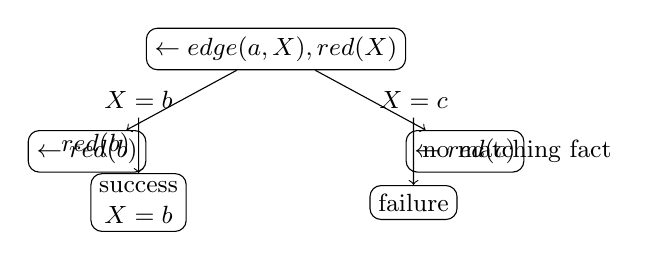
\begin{tikzpicture}[
  level distance=13mm,
  sibling distance=48mm,
  every node/.style={draw,rounded corners,align=center,font=\small,inner sep=3pt},
  edge from parent/.style={->,draw}]
\node {\(\leftarrow edge(a,X),red(X)\)}
  child {node {\(\leftarrow red(b)\)}
    edge from parent node[left,draw=none]{\(X=b\)}
    child {node {success\\\(X=b\)}
      edge from parent node[left,draw=none]{\(red(b)\)}}}
  child {node {\(\leftarrow red(c)\)}
    edge from parent node[right,draw=none]{\(X=c\)}
    child {node {failure}
      edge from parent node[right,draw=none]{no matching fact}}};
\end{tikzpicture}
\caption{An SLD tree for the facts \(edge(a,b)\), \(edge(a,c)\), and \(red(b)\).
The left branch returns the computed answer \(X=b\); the right branch finitely
fails.}
\label{fig:p09-sld-tree}
\end{figure}

\begin{hbdefinition}{def:p09-normal-program}{Normal programs and allowedness}
A normal clause is
\[
 H\leftarrow A_1,\ldots,A_m,
   \mathsf{not}\ B_1,\ldots,\mathsf{not}\ B_n,
\]
where \(H,A_i,B_j\) are non-equality predicate atoms and \(\mathsf{not}\) is
default negation, not classical negation.  The non-equality and ground-term
signature conventions of Definition~\ref{def:p09-definite-program} remain in
force.  A clause is \emph{admissible} when every variable in it occurs either
in the head or in a positive body atom.  It is \emph{allowed} when every
variable in it occurs in a positive body atom.  A query is allowed when every
variable in it occurs in a positive literal.

For a normal program \(P\) and query \(G\), the pair \(P\cup\{G\}\) is
\emph{allowed} when (i) every clause of \(P\) is admissible; (ii) every clause
defining a predicate that occurs positively in \(G\), or positively in the body
of any clause of \(P\), is allowed; and (iii) \(G\) is allowed.  Admissibility is
the weaker syntactic condition: a head-only variable may be admissible but is
not allowed.  Both terms classify syntax, not semantics, and the pair condition
is used below only for the nonfloundering and ground-answer conclusion
\cite[\S15, pp.~88--90]{Lloyd1987}.
\index{normal logic program}\index{allowed logic program}
\end{hbdefinition}

\begin{hbdefinition}{def:p09-sldnf}{SLDNF and negation as finite failure}
SLDNF uses the positive transition of
Definition~\ref{def:p09-sld}.  Selection is \emph{safe}: any positive literal
may be selected, but a negative literal may be selected only when its atom is
ground.  Safeness restricts the computation rule; it is distinct from the
allowedness condition on program and query syntax.  The mutually recursive
notions of refutation and finitely failed tree are stratified by a finite rank.
Rank \(0\) uses only positive selections; at rank \(k+1\), a selected ground
\(\mathsf{not}\ A\) succeeds by a finitely failed subsidiary tree for
\(\leftarrow A\) of rank at most \(k\), and it fails when such a subsidiary
goal has a refutation of rank at most \(k\).  An SLDNF refutation or finitely
failed tree has some finite rank.  The rank is a metalinguistic natural number,
not an object-language level; it is needed only to make these mutually recursive
definitions well founded.

A computation \emph{flounders} when it reaches a goal containing only
nonground negative literals, so safe selection has no available literal.  Thus
negation as failure is an operational finite-failure test, not classical
negation; divergence and floundering remain outcomes distinct from success and
finite failure \cite[\S15, pp.~84--89]{Lloyd1987}.
\index{negation as failure}\index{SLDNF}\index{floundering}
\end{hbdefinition}

\begin{hbdefinition}{def:p09-clark-completion}{Clark completion}
Suppose the clauses defining \(p\) have heads
\(p(\bar t_i)\) and bodies \(B_i\).  After renaming their local variables
\(\bar y_i\) apart, the completion contains
\[
 \forall\bar x\left(
 p(\bar x)\leftrightarrow
 \bigvee_i\exists\bar y_i\,
   (\bar x=\bar t_i\land B_i)
 \right),
\]
where each \(\mathsf{not}\ A\) in \(B_i\) is read as \(\neg A\), and an empty
disjunction is \(\bot\).  For the active finite signature \(\Sigma\), Clark's
equality theory is the following signature-relative axiom set:
\begin{enumerate}
\item equality is reflexive, symmetric, and transitive, and every function and
predicate respects it:
\[
\begin{gathered}
 \forall x\;x=x,\qquad
 \forall x\,y\;(x=y\to y=x),\\
 \forall x\,y\,z\;((x=y\land y=z)\to x=z),\\
 \bigwedge_i x_i=y_i\to f(\bar x)=f(\bar y),\qquad
 \bigwedge_i x_i=y_i\to
   \bigl(p(\bar x)\leftrightarrow p(\bar y)\bigr),
\end{gathered}
\]
with universal closure in the last two schemas;
\item distinct function symbols have disjoint ranges,
\[
 \forall\bar x\,\bar y\;f(\bar x)\ne g(\bar y)\qquad(f\ne g);
\]
\item every function symbol is coordinatewise injective,
\[
 \forall\bar x\,\bar y\;
 f(\bar x)=f(\bar y)\to\bigwedge_i x_i=y_i;
\]
\item the signature-relative acyclicity schema
\(\forall x\,\bar z\;t[x,\bar z]\ne x\) for every nonvariable finite term
\(t[x,\bar z]\) in which \(x\) occurs as a proper subterm.
\end{enumerate}
Constants are the nullary function symbols, so distinct constants are covered
by disjointness.  These axioms state the free finite-term-algebra behavior that
completion needs; they are object-language equality axioms, unlike the
metalinguistic unification operation in Definition~\ref{def:p09-sld}.  The
predicate biconditionals together with this explicit equality theory form
\(\operatorname{Comp}(P)\).  Completion closes the
definitions of predicates; it is not the least-model or stable-model
construction and can differ from both on recursive negation
\cite{Clark1978}.
\index{Clark completion}
\end{hbdefinition}

\begin{hbtheorem}{thm:p09-sldnf-completion}{cited=Lloyd1987}{Soundness and nonfloundering boundaries for SLDNF}
Let \(P\) be a normal program and let
\(G=\leftarrow L_1,\ldots,L_n\) be a normal query.  Under safe selection, every
computed SLDNF answer \(\theta\) satisfies
\[
 \operatorname{Comp}(P)\models
 \forall\bigl((L_1\land\cdots\land L_n)\theta\bigr),
\]
where \(\mathsf{not}\ A\) is read as \(\neg A\) and the universal closure binds
the variables remaining after \(\theta\).  If \(P\cup\{G\}\) has a finitely
failed SLDNF tree, then the universally closed goal clause
\(\neg(L_1\land\cdots\land L_n)\) is entailed by
\(\operatorname{Comp}(P)\).  In particular, finite failure of the ground query
\(\leftarrow A\) entails \(\operatorname{Comp}(P)\models\neg A\).

If \(P\cup\{G\}\) is allowed in the exact sense of
Definition~\ref{def:p09-normal-program}, no computation flounders and every
computed answer grounds all variables of \(G\).  These are soundness and
nonfloundering results, not completeness or termination for arbitrary normal
programs.  Lloyd's adjacent completeness theorem requires a map from predicate
symbols to nonnegative integers such that every predicate in a clause body has
strictly lower level than its head predicate; in particular, that hypothesis
excludes recursion \cite[\S\S14--16, thms.~15.4, 15.6, and 16.3]{Lloyd1987}.
\end{hbtheorem}

\begin{hbdefinition}{def:p09-stable-model}{Stable model of a finite normal program}
For the finite ground specialization of
Definition~\ref{def:p09-normal-program} and a set \(M\) of its atoms, the
Gelfond--Lifschitz reduct \(P^M\) deletes each rule containing
\(\mathsf{not}\ A\) with \(A\in M\), then deletes every remaining
default-negated literal.  The set \(M\) is a \emph{stable model} when it is the
least model of the resulting positive program \(P^M\).  The term is needed
because default negation and classical negation have different standings; it
 denotes a two-valued model relation, differs from completion on recursive
 negation, and is used by answer-set programming
 \cite{GelfondLifschitz1988,Lifschitz2008TwelveDefinitions}.  A nonground
 program denotes this construction
 only through an explicitly declared ground instantiation; the finite
 complexity theorem below does not cover infinite groundings.
\index{stable-model semantics}\index{answer-set programming}
\end{hbdefinition}

\begin{hbtheorem}{thm:p09-stable-complexity}{cited=DantsinEiterGottlobVoronkov2001}{Complexity of finite normal stable models}
For finite propositional normal programs, stable-model existence and credulous
atom consequence are \(\mathsf{NP}\)-complete; skeptical atom consequence is
\(\mathsf{coNP}\)-complete.  Verification of one proposed stable model is
polynomial because its reduct is positive.  Disjunctive heads have a different
complexity and are not covered \cite{MarekTruszczynski1999}.
\end{hbtheorem}

\begin{hbdefinition}{def:p09-well-founded}{Alternating fixed point for a finite ground normal program}
Let \(\Gamma_P(M)\) be the least model of the reduct \(P^M\).
\(\Gamma_P\) is antimonotone, so \(\Gamma_P^2\) is monotone.  Put
\[
 L=\operatorname{lfp}(\Gamma_P^2),
 \qquad
 G=\operatorname{gfp}(\Gamma_P^2).
\]
The well-founded interpretation makes atoms in \(L\) true, atoms outside
\(G\) false, and atoms in \(G\setminus L\) undefined.  This is a
three-valued semantic object, not a failed attempt to choose one stable model.
\index{well-founded semantics}\index{alternating fixed point}
\end{hbdefinition}

\begin{hbtheorem}{thm:p09-well-founded-properties}{cited=VanGelderRossSchlipf1991}{Well-founded approximation and computation}
The interpretation of Definition~\ref{def:p09-well-founded} is unique and is
computable in polynomial time for finite ground programs.  Every stable model
\(M\) satisfies \(L\subseteq M\subseteq G\); hence it extends every
well-founded true and false assignment.  If \(L=G\), this total interpretation
is the unique stable model.
\end{hbtheorem}

\begin{hbdefinition}{def:p09-conjunctive-query}{Conjunctive queries and canonical databases}
Over a finite relational database signature, a \(k\)-ary conjunctive query is
\[
 q(\bar x)=\exists\bar y\,
   \bigwedge_{j=1}^{m}R_j(\bar z_j),
\]
where the displayed tuples use variables from \(\bar x,\bar y\) and may use
declared constants; the equality-free convention is in force.  It is Boolean
when \(k=0\).  For a finite instance \(D\), a tuple \(\bar a\) is in \(q(D)\)
exactly when an assignment sending \(\bar x\) to \(\bar a\) makes every atom a
fact of \(D\).

The canonical database \(D_q\) has the variables and constants of \(q\) as its
elements, one relation fact for each query atom, and distinguished tuple
\(\bar x\).  Homomorphisms fix declared constants.  This object is necessary
to turn query evaluation and containment into typed homomorphism problems; it
is a finite structure with a distinguished tuple and is used in the next
theorem.
\index{conjunctive query}\index{canonical database}
\end{hbdefinition}

\begin{hbtheorem}{thm:p09-chandra-merlin}{cited=ChandraMerlin1977}{Chandra--Merlin homomorphism theorem}
For every finite instance \(D\) and tuple \(\bar a\),
\(\bar a\in q(D)\) exactly when there is a homomorphism
\(D_q\to D\) carrying the distinguished tuple to \(\bar a\).  For
conjunctive queries \(q_1,q_2\) of the same arity,
\[
 q_1\subseteq q_2
 \quad\Longleftrightarrow\quad
 \text{there is a homomorphism }D_{q_2}\to D_{q_1}
 \text{ aligning their distinguished tuples}.
\]
\end{hbtheorem}

Vardi's presentation separates data, expression, and combined complexity; it
controls that input-measure distinction rather than both bounds below
\cite{Vardi1982}.  The two theorem identities are nonredundant because the
first fixes the query and varies only the database, whereas the second varies
both objects.

\begin{hbtheorem}{thm:p09-cq-data-evaluation}{cited=AbiteboulHullVianu1995}{Fixed-query conjunctive-query data complexity}
Under the standard finite relational encoding, evaluation of each fixed
conjunctive query is in \(\mathsf{AC}^{0}\) data complexity.  The formula is
fixed and only the finite database instance varies.
\end{hbtheorem}

\begin{hbtheorem}{thm:p09-cq-combined-evaluation}{cited=ChandraMerlin1977}{Combined conjunctive-query evaluation complexity}
Boolean conjunctive-query evaluation is \(\mathsf{NP}\)-complete when the query
and finite database instance are both input.  This combined problem is not the
fixed-query problem of Theorem~\ref{thm:p09-cq-data-evaluation}.
\end{hbtheorem}

\begin{hbtheorem}{thm:p09-cq-containment}{cited=ChandraMerlin1977}{Conjunctive-query containment complexity}
Containment of two equality-free conjunctive queries of the same arity is
\(\mathsf{NP}\)-complete under the finite relational encoding.  The decision
test uses the reverse canonical-database homomorphism in
Theorem~\ref{thm:p09-chandra-merlin}; it is a query-to-query problem, not data
evaluation with one query fixed.
\end{hbtheorem}

\begin{hbdefinition}{def:p09-datalog}{Datalog programs and evaluation}
A Datalog program is a finite function-free set of definite clauses over
extensional database predicates and intensional predicates.  Every variable in
a rule head occurs in its positive body.  Given a finite database \(D\), the
active domain consists of constants in \(D\) or the program.  Starting with the
extensional facts, the immediate-consequence operator adds ground intensional
heads whose bodies already hold; because the active Herbrand base is finite,
iteration reaches its least fixed point after finitely many additions.  A
designated intensional atom or tuple is the query output.  This finite
least-fixed-point evaluation is distinct from SLD search order and is used by
the following complexity result.
\index{Datalog}\index{data complexity}\index{combined complexity}
\end{hbdefinition}

\begin{hbtheorem}{thm:p09-datalog-complexity}{cited=DantsinEiterGottlobVoronkov2001}{Datalog data and combined complexity}
Every fixed Datalog program and query has polynomial-time data complexity, and
some fixed Datalog query has \(\mathsf P\)-complete evaluation under logspace
many-one reductions as the extensional database varies.  Evaluation is
\(\mathsf{EXPTIME}\)-complete in combined complexity when program, query, and
database are all input.  General Datalog query containment is undecidable;
the decidable \(\mathsf{NP}\)-complete containment result in
Theorem~\ref{thm:p09-cq-containment} concerns conjunctive queries, not arbitrary
recursive Datalog programs.
\end{hbtheorem}

\begin{table}[htbp]
\centering\scriptsize
\begin{tabularx}{\textwidth}{@{}l X X X@{}}
\toprule
Presentation & Exact input and standing & Success/model criterion & Boundary \\
\midrule
Definite program / SLD & first-order definite clauses and a selected goal &
empty-goal refutation with computed answer; complete under fair enumeration &
may diverge even when no refutation exists \\
Pure Prolog search & leftmost literal, textual clause order, depth-first
backtracking & first success reached by that operational traversal & may
diverge before an existing SLD refutation; cut and non-finite-term unification
are outside Theorem~\ref{thm:p09-sld-adequacy} \\
Clark completion / SLDNF & normal clauses with safe literal selection;
allowedness separately guarantees nonfloundering and ground answers &
default negation succeeds only by finite failure of a ground subsidiary tree &
may flounder or diverge; no arbitrary-program completeness \\
Well-founded semantics & finite ground normal program &
one polynomial-time three-valued alternating fixed point &
undefined atoms need not receive a two-valued choice \\
Stable semantics & finite ground normal program &
\(M=\operatorname{lfp}(T_{P^M})\); zero, one, or many stable models &
existence/credulous \(\mathsf{NP}\)-complete; skeptical
\(\mathsf{coNP}\)-complete \\
Datalog & finite safe function-free positive rules over a finite database &
finite least-fixed-point saturation &
polynomial data for each fixed query, with a fixed \(\mathsf P\)-complete
query; \(\mathsf{EXPTIME}\)-complete combined \\
\bottomrule
\end{tabularx}
\caption{Operational and model-theoretic boundaries for logic programming and
Datalog.  The rows differ in syntax, result object, and failure behavior; no
single use of \emph{negation} or \emph{fixed point} identifies them.}
\label{tab:p09-logic-programming}
\end{table}

\begin{hbdefinition}{def:p09-csp}{Finite-template constraint satisfaction}
For finite relational structures \(A,B\) of the same signature, a
constraint-satisfaction instance asks whether a homomorphism \(A\to B\)
exists.  In \(\operatorname{CSP}(B)\), the finite template \(B\) is fixed and
only \(A\) is input.  Fixing the template is necessary: it is the parameter
whose algebraic polymorphisms classify the problem, and it distinguishes the
family below from unrestricted combined homomorphism.
\index{constraint-satisfaction problem}\index{finite template}
\end{hbdefinition}

\begin{hbtheorem}{thm:p09-csp-dichotomy}{cited=Zhuk2020}{Finite-domain CSP dichotomy}
For every fixed finite relational template \(B\),
\(\operatorname{CSP}(B)\) is either solvable in polynomial time or is
\(\mathsf{NP}\)-complete.  The theorem classifies each fixed-template problem;
it does not assert that unrestricted finite homomorphism is tractable.
\end{hbtheorem}

% Source presentations for register row N-c-022.

\subsection{From declarative clauses to SLD search and finite failure}
\label{sec:p09-presentation-n-c-022}

\subsubsection{One relation, two modes, and three kinds of control}

Kowalski's procedural reading starts from clauses, not from a separately
specified input--output function.  For a concrete source-faithful example, use
\([\,]\) for the empty list and \([u\mid v]\) for
\(\operatorname{cons}(u,v)\), and let
\[
\begin{array}{rcl}
 \mathit{app}([\,],Y,Y)&\leftarrow&\\
 \mathit{app}([U\mid X],Y,[U\mid Z])
   &\leftarrow&\mathit{app}(X,Y,Z).
\end{array}
\]
These are universally quantified definite clauses defining one ternary
relation.  Calling the first two arguments \enquote{inputs} and the third an
\enquote{output} describes one use of that relation; it is not part of the
logical clause.

In the forward mode, the goal
\(\leftarrow\mathit{app}([a,b],[c],Z)\) has the refutation
\[
\begin{aligned}
 \leftarrow\mathit{app}([a,b],[c],Z)
 &\Longrightarrow
 \leftarrow\mathit{app}([b],[c],Z_1)
   &&[Z=[a\mid Z_1]],\\
 &\Longrightarrow
 \leftarrow\mathit{app}([\,],[c],Z_2)
   &&[Z_1=[b\mid Z_2]],\\
 &\Longrightarrow\Box
   &&[Z_2=[c]].
\end{aligned}
\]
The computed answer is \(Z=[a,b,c]\).  In the inverse mode, the same two
clauses enumerate every split of a fixed list.  The complete branching
calculation for
\(\leftarrow\mathit{app}(X,Y,[a,b])\) is
\[
\begin{array}{rcll}
 \leftarrow\mathit{app}(X,Y,[a,b])
 &\Longrightarrow&\Box
   &[X=[\,],\ Y=[a,b]],\\
 &\Longrightarrow&
   \leftarrow\mathit{app}(X_1,Y,[b])
   &[X=[a\mid X_1]],\\[2pt]
 \leftarrow\mathit{app}(X_1,Y,[b])
 &\Longrightarrow&\Box
   &[X_1=[\,],\ Y=[b]],\\
 &\Longrightarrow&
   \leftarrow\mathit{app}(X_2,Y,[\,])
   &[X_1=[b\mid X_2]],\\[2pt]
 \leftarrow\mathit{app}(X_2,Y,[\,])
 &\Longrightarrow&\Box
   &[X_2=[\,],\ Y=[\,]].
\end{array}
\]
At the last node the recursive head does not unify with an empty third list, so
it contributes no child to the complete tree.
Thus the three successful answers are
\[
 (X,Y)=([\,],[a,b]),\qquad([a],[b]),\qquad([a,b],[\,]).
\]
This is the relational use of variables as partially specified data emphasized
in the early procedural presentation.  The complete member computation in
Kowalski supplies the original branching precedent; the append relation is the
worked source example in the later semantic and SLD developments
\cite[printed pp.~570--573]{Kowalski1974}
\cite{VanEmdenKowalski1976,AptVanEmden1982}.

Three choices must remain separate.
\begin{enumerate}
\item An \emph{atom-selection rule} chooses one atom of the current goal.
\item A \emph{clause choice} chooses one unifying program-clause head and hence
  one child of the complete tree.
\item A \emph{tree-search strategy} decides which pending child to visit next.
\end{enumerate}
The first is the computation rule quantified over by the SLD completeness
theorem.  The second creates logical nondeterminism.  The third includes
breadth-first, fair interleaving, and Prolog's depth-first backtracking.
Kowalski's paper supplies the procedural reading and the computation-space
examples; it does not identify any one traversal with logical consequence.

\subsubsection{Herbrand interpretations and the immediate-consequence proof}

Fix a first-order signature with at least one ground term.  Its \emph{Herbrand
universe} is the set of all ground terms over that signature, and its
\emph{Herbrand base} is the set of all ground predicate atoms over that
universe.  A ground instance of a clause is obtained by replacing every
variable with a ground term.  Consequently a Herbrand interpretation is exactly
a subset \(I\) of the Herbrand base: a ground atom is true precisely when it
belongs to \(I\).

For a definite program \(P\), Definition~\ref{def:p09-definite-program} gives
\[
 T_P(I)=
 \{\,H\theta:
   (H\leftarrow B_1,\ldots,B_k)\in P,\ 
   \theta\text{ ground},\
   B_i\theta\in I\text{ for all }i\,\}.
\]
This is a semantic operator on sets of ground atoms.  It is not one SLD
transition: it applies every ground clause instance simultaneously.

The finite ancestor program makes the iteration visible:
\[
\begin{array}{ll}
 parent(a,b).&parent(b,c).\\
 anc(X,Y)\leftarrow parent(X,Y).&
 anc(X,Z)\leftarrow parent(X,Y),anc(Y,Z).
\end{array}
\]
Starting from the empty interpretation,
\[
\begin{aligned}
 T_P^1(\varnothing)
   &=\{parent(a,b),parent(b,c)\},\\
 T_P^2(\varnothing)
   &=T_P^1(\varnothing)
     \cup\{anc(a,b),anc(b,c)\},\\
 T_P^3(\varnothing)
   &=T_P^2(\varnothing)\cup\{anc(a,c)\},\\
 T_P^4(\varnothing)&=T_P^3(\varnothing).
\end{aligned}
\]
The consequence \(anc(a,c)\) appears independently of a clause order, selected
goal atom, or search traversal.

The least-model theorem follows from four explicit steps.

\paragraph{Monotonicity.}
If \(I\subseteq J\), every ground clause body contained in \(I\) is contained
in \(J\), so \(T_P(I)\subseteq T_P(J)\).

\paragraph{Models are exactly pre-fixed points.}
A Herbrand interpretation \(I\) satisfies every ground instance
\[
 H\leftarrow B_1,\ldots,B_k
\]
exactly when membership of all \(B_i\) in \(I\) implies membership of \(H\).
This is precisely \(T_P(I)\subseteq I\).

\paragraph{The union of the finite stages is a fixed point.}
Put
\[
 L=\bigcup_{n<\omega}T_P^n(\varnothing).
\]
Every clause body is finite.  If all its atoms belong to \(L\), there is one
finite stage containing all of them: take the maximum of their finitely many
stage indices.  Hence
\[
 T_P(L)
 =\bigcup_{n<\omega}T_P(T_P^n(\varnothing))
 =\bigcup_{n<\omega}T_P^{n+1}(\varnothing)
 =L.
\]

\paragraph{It is the least model.}
If \(I\) is any Herbrand model, then \(T_P(I)\subseteq I\).  Induction on \(n\)
gives \(T_P^n(\varnothing)\subseteq I\) for every \(n\), and therefore
\(L\subseteq I\).  Since \(L\) is itself a fixed point and hence a model, it is
the least Herbrand model:
\[
 M_P=L=\operatorname{lfp}(T_P).
\]
For a ground atom \(A\), ordinary first-order consequence agrees with
membership in this least model: by the Herbrand theorem, failure of ground
consequence has a Herbrand countermodel, while the intersection of the
Herbrand models of a definite program is itself its least model
\cite[printed pp.~736--741]{VanEmdenKowalski1976}.

The finite-stage statement has an equally concrete proof-tree form.  A
\emph{ground proof tree} for \(A\) has root \(A\); an internal node labelled
\(H\) chooses a ground clause instance
\(H\leftarrow B_1,\ldots,B_k\) and has the \(B_i\) as children; a fact is a
leaf.  Taking a fact-only tree to have height \(1\), induction on \(n\) proves
\[
 A\in T_P^n(\varnothing)
 \quad\Longleftrightarrow\quad
 A\text{ has a ground proof tree of height at most }n.
\]
The forward induction reads the clause instance that put \(A\) into the next
stage.  The reverse induction applies \(T_P\) after all child roots have
appeared.  Thus every member of \(M_P\) has a finite proof, even when the
program or Herbrand base is infinite; there need not be one uniform finite
height for all consequences.

\subsubsection{SLD answers: soundness, lifting, and strong completeness}

Now return to goal-directed proof.  Standardize every input clause apart before
unification.  For the goal \(\leftarrow anc(a,Z)\), choose the recursive clause
first:
\[
\begin{aligned}
 \leftarrow anc(a,Z)
 &\xRightarrow{\theta_1}
   \leftarrow parent(a,Y_0),anc(Y_0,Z),
 &\theta_1&=\{X_0/a,\ Z_0/Z\},\\
 &\xRightarrow{\theta_2}
   \leftarrow anc(b,Z),
 &\theta_2&=\{Y_0/b\},\\
 &\xRightarrow{\theta_3}
   \leftarrow parent(b,Z),
 &\theta_3&=\{X_1/b,\ Y_1/Z\},\\
 &\xRightarrow{\theta_4}\Box,
 &\theta_4&=\{Z/c\}.
\end{aligned}
\]
Here \((X_0,Y_0,Z_0)\) and \((X_1,Y_1)\) belong to fresh variants of the two
clauses.  Restricting the composed substitution to the initial variable gives
the computed answer \(Z=c\).  The root branch using the base clause instead
returns \(Z=b\).

\paragraph{Why every computed answer is correct.}
At one positive SLD step, the selected goal atom \(A_i\) is unified with the
head \(H\) of
\[
 H\leftarrow B_1,\ldots,B_k.
\]
The universally closed clause entails
\(B_1\land\cdots\land B_k\to H\).  After applying the mgu \(\theta\), the
conjunction of the new resolvent therefore entails the conjunction of the old
goal under \(\theta\).  Chaining these implications through a refutation and
using that the empty conjunction is true yields
\[
 P\models
 \forall\bigl((A_1\land\cdots\land A_n)
              \theta_1\cdots\theta_m\bigr).
\]
After restriction to the variables of the initial goal, this is exactly the
correct-answer condition in Definition~\ref{def:p09-sld}.  Apt and van Emden's
fixed-point proof sharpens the same invariant.  If \(G_{m-i}\) is the goal
\(i\) steps before success and \(\theta_{m-i+1},\ldots,\theta_m\) are the
remaining substitutions, then every ground instance of every atom in
\(G_{m-i}\theta_{m-i+1}\cdots\theta_m\) belongs to
\(T_P^i(\varnothing)\)
\cite[thm.~5.1 and cor.~5.2]{AptVanEmden1982}.

\paragraph{The lifting step.}
Suppose an instance \(G\eta\) takes an SLD step using a standardized-apart
clause \(C\) whose variables are disjoint from those of \(G\eta\), and write
\(\sigma\) for the mgu used in that step.  Then \(\eta\sigma\) unifies the
selected atom of \(G\) with the uninstantiated clause head.  If \(\theta\) is
an mgu of those two atoms, the defining property of an mgu gives a substitution
\(\rho\) through which this unifier factors:
\[
 (\eta\sigma)|_{\operatorname{Var}(G)\cup\operatorname{Var}(C)}
 =
 (\theta\rho)|_{\operatorname{Var}(G)\cup\operatorname{Var}(C)}.
\]
The resolvent from \(G\) under \(\theta\) therefore has the resolvent from
\(G\eta\) under \(\sigma\) as a further instance.  Repeating this argument
lifts every finite refutation of an instance to a refutation of the original
goal.  If \(\sigma_1,\ldots,\sigma_m\) are the mgus in the instance
refutation and \(\theta_1,\ldots,\theta_m\) those in the lifted refutation, the
general factorization is
\[
 \eta\sigma_1\cdots\sigma_m
   =(\theta_1\cdots\theta_m)\rho
\]
on the variables of the initial goal.  In the special case used below, the
instance refutation has the identity as its computed answer, and the left side
reduces there to \(\eta\).  This is why completeness says that every correct
answer is an \emph{instance} of a computed answer; the two substitutions need
not be literally equal.

\paragraph{From the least model to a refutation.}
For a ground atom \(A\in M_P\), choose the least stage at which \(A\) appears.
The corresponding ground clause has body atoms at earlier stages.  Induction
on that stage constructs finite refutations of those body goals.  The lifting
lemma replaces the ground clause instances by standardized-apart clauses and
mgus.  For a finite conjunction, the same induction combines the component
refutations.  Thus a semantically correct ground instance has an SLD
refutation.

For a non-ground correct answer \(\eta\), the universal closure of each
instantiated goal atom follows from \(P\).  Replace its remaining variables by
distinct constants occurring in neither \(P\) nor \(G\eta\).  Ground
completeness gives refutations for those ground atoms; replacing the fresh
constants back by variables gives
refutations of the atoms in \(G\eta\) whose computed answers are the identity.
Combine them into a refutation of \(G\eta\), then apply the lifting lemma.  The
result has computed answer \(\theta\) and a further substitution \(\rho\) such
that \(\eta=\theta\rho\) on the initial variables.  Finally, the switching lemma
permutes adjacent independent atom selections; repeated switching transforms a
refutation into one following any fixed computation rule, without changing the
answer except for variants.  This is the proof spine behind Lloyd's Theorems
9.2--9.5 and the exact strong answer theorem stated in
Theorem~\ref{thm:p09-sld-adequacy}
\cite[ch.~2, \S\S8--9]{Lloyd1987}.

\paragraph{What the theorem does not say.}
Consider the extensionally equivalent left-recursive presentation
\[
\begin{array}{rcl}
 anc(X,Y)&\leftarrow&anc(X,Z),parent(Z,Y),\\
 anc(X,Y)&\leftarrow&parent(X,Y),
\end{array}
\]
with the two parent facts above and the recursive clause placed first.  The
complete SLD tree for \(\leftarrow anc(a,Y)\) has a base-clause branch
\[
 \leftarrow parent(a,Y)\Longrightarrow\Box\quad[Y=b].
\]
Its first recursive branch begins
\[
\begin{aligned}
 \leftarrow anc(a,Y)
 &\Longrightarrow
 \leftarrow anc(a,Z_1),parent(Z_1,Y)\\
 &\Longrightarrow
 \leftarrow anc(a,Z_2),parent(Z_2,Z_1),parent(Z_1,Y)\\
 &\Longrightarrow\cdots .
\end{aligned}
\]
A leftmost, textual-clause-order, depth-first traversal remains on this infinite
branch and never visits the existing answer.  The computation rule selected the
leftmost atom; clause order chose the recursive child; depth-first traversal
caused starvation.  Strong completeness says that the complete tree for the
fixed atom-selection rule contains a refutation.  It does not say that an
unfair traversal finds it
\cite[\S6, discussion after thm.~6.6]{AptVanEmden1982}.

\subsubsection{Completion and a proof from a finitely failed tree}

Clark completion changes one-way program clauses into classical definitions.
For clauses \(p(\bar t_i)\leftarrow B_i\), with local variables renamed apart,
Definition~\ref{def:p09-clark-completion} gives
\[
 p(\bar x)\leftrightarrow
 \bigvee_i\exists\bar y_i\,
   (\bar x=\bar t_i\land B_i),
\]
together with the displayed free-term equality theory.  The equality axioms
matter: they make distinct constructors disjoint, make each constructor
injective, exclude a finite term from containing itself, and justify the mgu
cases in the finite-tree proof.  Metalinguistic unification and object-language
equality in the completion remain different things.

For the parent/ancestor program, the completed definitions simplify to
\[
\begin{aligned}
 parent(x,y)
 &\leftrightarrow
   ((x=a\land y=b)\lor(x=b\land y=c)),\\
 anc(x,z)
 &\leftrightarrow
   \bigl(parent(x,z)\lor
   \exists y\,(parent(x,y)\land anc(y,z))\bigr).
\end{aligned}
\]
The complete SLD tree for the ground goal
\(\leftarrow anc(c,a)\) is finite and has no success leaf:
\[
\begin{array}{c}
 \leftarrow anc(c,a)\\[2pt]
 \swarrow\hspace{45mm}\searrow\\[-2pt]
 \leftarrow parent(c,a)
 \hspace{20mm}
 \leftarrow parent(c,Y_1),anc(Y_1,a)\\
 \text{failure}\hspace{42mm}\text{failure at }parent(c,Y_1).
\end{array}
\]
The two root children come from the two ancestor clauses.  At each leaf, no
parent fact unifies with a first argument \(c\).

The completion proves the same negative conclusion.  Free-term equality gives
\(c\ne a\) and \(c\ne b\), so the parent biconditional entails
\(\forall y\,\neg parent(c,y)\).  Both disjuncts in the ancestor
biconditional are therefore false at \((c,a)\), whence
\[
 \operatorname{Comp}(P)\models\neg anc(c,a).
\]
This is not an appeal to elapsed search time: it uses every child of the root
and the fact that the whole tree is finite.

The general soundness proof has the same shape.  At a positive selected atom,
the completion and equality axioms entail the goal clause at a failed leaf when
there is no unifying head; at an internal node they entail the parent goal
clause from the conjunction of all child goal clauses.  Induction on tree depth
therefore propagates failure from every leaf to the root.  With negative
literals, an outer induction on the finite SLDNF rank handles subsidiary trees:
a subsidiary refutation proves its ground atom, while a subsidiary finite
failure proves its classical negation in the completion.  This is the
rank-then-depth proof of Lloyd's Theorem 15.4, whose positive core is Clark's
finite-failure argument
\cite{Clark1978}\cite[thm.~15.4]{Lloyd1987}.

Finiteness is load-bearing.  Add only the clause
\[
 loop(X)\leftarrow loop(X).
\]
The goal \(\leftarrow loop(a)\) has one infinite branch and neither a refutation
nor a finite failed tree.  Its completed definition is the tautology
\(\forall x\,(loop(x)\leftrightarrow loop(x))\), which entails neither
\(loop(a)\) nor \(\neg loop(a)\).
Thus \enquote{no answer has appeared} cannot be substituted for finite failure.

\subsubsection{Ground SLDNF, four outcomes, and the exact theorem boundary}

Use the normal program
\[
\begin{array}{rcl}
 bird(tweety)&\leftarrow&\\
 flies(X)&\leftarrow&bird(X),\mathsf{not}\ abnormal(X),\\
 loop(X)&\leftarrow&loop(X).
\end{array}
\]
There is no clause defining \(abnormal\).  The registered safe SLDNF rule
selects a negative literal only after its atom is ground.  Its mutually
recursive success and failure definitions are well-founded by the finite rank
from Definition~\ref{def:p09-sldnf}.

For \(\leftarrow flies(tweety)\), positive resolution first gives
\[
 \leftarrow bird(tweety),\mathsf{not}\ abnormal(tweety)
 \Longrightarrow
 \leftarrow\mathsf{not}\ abnormal(tweety).
\]
The subsidiary rank-\(0\) tree for
\(\leftarrow abnormal(tweety)\) is the one-node finite failed tree, so the
ground negative literal succeeds at rank \(1\), and the outer goal refutes.  No
variable binding is returned by the negative step; negation as failure is a
test.

The four operational outcomes can now be separated without euphemism:
\begin{center}
\begin{tabularx}{\textwidth}{@{}l X X@{}}
\toprule
Goal & Subsidiary behavior & Outer result \\
\midrule
\(\leftarrow\mathsf{not}\ abnormal(tweety)\)
  & The ground positive goal has a finite complete tree with no success.
  & Negative success; completion entails
    \(\neg abnormal(tweety)\). \\
\(\leftarrow\mathsf{not}\ bird(tweety)\)
  & The ground positive goal has a refutation using the fact.
  & Negative failure; no negative answer is returned. \\
\(\leftarrow\mathsf{not}\ loop(tweety)\)
  & The ground positive goal follows one infinite recursive branch.
  & Divergence; neither negative success nor negative failure. \\
\(\leftarrow\mathsf{not}\ parent(X,b)\)
  & The negative atom is nonground and no positive literal remains to bind it.
  & Floundering under safe selection; neither success nor failure. \\
\bottomrule
\end{tabularx}
\end{center}

Safeness and allowedness have different standings.  Safeness is a restriction
on which literal the computation rule may select.  Allowedness is the syntactic
condition in Definition~\ref{def:p09-normal-program}.  The flies clause above
is allowed because its variable occurs in the positive body atom \(bird(X)\).
The floundering query is not allowed because \(X\) occurs only in a negative
literal.  Lloyd's Proposition 15.1 says that if the whole program/query pair is
allowed, no computation flounders and every computed answer grounds the
original query variables.  This is a sufficient syntactic guarantee, not the
definition of SLDNF success and not a hypothesis of the two soundness theorems.

Theorem 15.4 says that a finitely failed safe SLDNF tree makes the universally
closed goal clause a consequence of \(\operatorname{Comp}(P)\).  Theorem 15.6
says that every safe SLDNF computed answer is a correct completion answer.  Its
proof inducts on refutation length; positive steps use the completed defining
biconditional and negative steps use Theorem 15.4.  Neither theorem claims
termination or completeness for every normal program
\cite[\S15, prop.~15.1 and thms.~15.4, 15.6]{Lloyd1987}.

The adjacent completeness theorem has much stronger hypotheses.  A
hierarchical program has a natural-number level for each predicate such that
every body predicate has strictly smaller level than its clause head.  This
excludes both \(anc\) recursion and \(loop\).  Under that hypothesis,
allowedness, and a safe computation rule, Lloyd's Theorem 16.3 proves that the
SLDNF tree exists and is finite and that every ground correct completion answer
is computed.  Its termination proof orders each goal by the finite multiset of
predicate levels; every child strictly decreases that well-founded multiset.
This theorem cannot be relabelled as completeness for arbitrary recursive
normal programs \cite[thm.~16.3]{Lloyd1987}.

The internal SLDNF locators were checked in a university-hosted scan of the
corrected printing against the Springer edition record; the scan is not a
publisher-hosted copy, so that provenance remains explicit.  Concrete Prolog
is commonly presented with leftmost selection, textual clause order, and
depth-first traversal; it also provides cut and arithmetic, and some
implementations use unification without the occurs check \cite{Lloyd1987}.
The confirmed ISO
general-core record and public WG17 material separately identify control
constructs, cut, arithmetic, negation as failure, ordinary unification, and
unification with an occurs check as subjects addressed separately.  The
corrected normative clauses are not part of the available source basis, so no
clause-exact ISO behavior is asserted.  In every case these implementation and
language-standard choices do not alter the pure SLD theorem; they fall outside it unless separately
formalized \cite{ISO13211-1-1995}.

% Source presentations for register row N-c-023.

\subsection{Stable models as candidate-dependent reducts}
\label{sec:p09-presentation-n-c-023}

\subsubsection{The Gelfond--Lifschitz construction by complete calculation}

A finite ground normal rule has the form
\[
 H\leftarrow A_1,\ldots,A_m,
   \mathsf{not}\ B_1,\ldots,\mathsf{not}\ B_n,
\]
where all displayed expressions other than \(\mathsf{not}\) are ground atoms.
Let \(\operatorname{At}(P)\) be the finite set of atoms occurring in a finite
ground program \(P\), and let \(M\subseteq\operatorname{At}(P)\) be a candidate
interpretation.  Unlike the full Herbrand base, \(\operatorname{At}(P)\) is only
this syntactically occurring finite set; atoms outside it cannot be generated by
a reduct and hence cannot belong to a stable model.  The reduct \(P^M\) is
formed rule by rule:
\begin{enumerate}
\item delete the rule if \(B_j\in M\) for at least one \(j\);
\item otherwise retain its head and positive body and erase all
  \(\mathsf{not}\ B_j\).
\end{enumerate}
The result is a positive definite program.  Therefore it has the unique least
model
\[
 \Gamma_P(M)=\operatorname{lfp}(T_{P^M}),
\]
and Definition~\ref{def:p09-stable-model} says exactly
\[
 M\text{ is stable}
 \quad\Longleftrightarrow\quad
 M=\Gamma_P(M).
\]
Thus the least fixed point is taken only \emph{after} the candidate-dependent
deletion step.  It is not an iteration of one monotone operator that directly
assigns a model to the original normal program.

The map reverses inclusion.  If \(M\subseteq N\), every rule retained in
\(P^N\) is retained in \(P^M\), so \(P^N\subseteq P^M\) and
\(\Gamma_P(N)\subseteq\Gamma_P(M)\).  This antimonotonicity is why the adjacent
well-founded construction uses the monotone composite \(\Gamma_P^2\); it does
not give \(\Gamma_P\) itself a least fixed point.

For a nonground rule, the standing of the construction is equally explicit:
first take its declared ground instances and only then form the reduct.  If
function symbols generate infinitely many ground terms, the finite decision
arguments below no longer apply.  If the program is function-free and its
constants are finite, its grounding is finite.

For the program
\[
 P=\{p\leftarrow\mathsf{not}\ q,\quad
     q\leftarrow\mathsf{not}\ p\},
\]
the candidate dependence is visible by checking all four candidates:
\[
\begin{array}{c|c|c}
M&P^M&\operatorname{lfp}(T_{P^M})\\
\hline
\varnothing&\{p\leftarrow,\ q\leftarrow\}&\{p,q\}\\
\{p\}&\{p\leftarrow\}&\{p\}\\
\{q\}&\{q\leftarrow\}&\{q\}\\
\{p,q\}&\varnothing&\varnothing
\end{array}
\]
Hence the stable models are exactly \(\{p\}\) and \(\{q\}\).  In contrast,
\[
 P'=\{p\leftarrow\mathsf{not}\ p\}
\]
has none: the empty candidate produces the fact \(p\), while the candidate
\(\{p\}\) deletes the only rule and produces the empty least model.  These
calculations establish both nonuniqueness and nonexistence without importing a
solver.

For a positive definite program \(Q\), the reduct is \(Q\) for every candidate,
so \(\Gamma_Q(M)=M_Q\) for every \(M\).  Consequently
\[
 M\text{ is a stable model of }Q
 \quad\Longleftrightarrow\quad M=M_Q.
\]
This is the precise adjacent case connecting stable semantics to
Definition~\ref{def:p09-definite-program}; it does not turn a program with
default negation into a monotone fixed-point construction.

Every stable model is an ordinary two-valued model of its program and, more
strongly, a minimal Herbrand model.  This is Theorem~1 of the original paper.
For ordinary modelhood, a rule deleted from the reduct has a false
default-negated body condition in the candidate, while a retained rule is
satisfied because the candidate models its positive reduct.  For minimality,
suppose that a proper subset \(N\subsetneq M\) were also a Herbrand model of
the original program.  Every rule retained in \(P^M\) came from a rule whose
default-negated atoms are outside \(M\), hence outside \(N\).  Since \(N\)
models that original rule, it models the retained positive rule.  Thus \(N\)
would be a model of \(P^M\), contradicting that \(M\) is the least model of
\(P^M\) \cite[\S2, thm.~1]{GelfondLifschitz1988}.

The converse fails, and stable semantics is not Clark completion.  For
\[
 R=\{p\leftarrow p\},
\]
every reduct is \(R\), whose least model is \(\varnothing\); hence
\(\varnothing\) is the unique stable model.  The completion is instead the
tautology \(p\leftrightarrow p\), which has both classical interpretations
\(\varnothing\) and \(\{p\}\).  The extra classical model \(\{p\}\) is
self-supported rather than generated by the positive least-model construction
\cite{GelfondLifschitz1988}.

The live first-party publication page still identifies the 1988 paper and
points to Lifschitz's former author-hosted PostScript file.  That dead link has
an archived capture containing the complete eleven-page author copy
corresponding to published pp.~1070--1080.  All eleven pages, including the
proofs supplied for
Theorems~1 and~3 and the intervening lemma, have now been inspected.
Section~2 first calls the fixed points above \emph{stable
sets}; after Theorem~1 proves minimality, it licenses the name \emph{stable
models}.  The paper then reserves the formulation \emph{the stable model
semantics is defined for \(P\)} for the case in which \(P\) has exactly one
stable model, which it declares canonical.  The broader modern convention used
in this handbook speaks of the stable-model relation even when a program has
zero or several stable models.  The reduct is unchanged; only the later
terminology has widened.  Lifschitz's retrospective independently reproduces
that reduct as Definition~C, including grounding before the two deletion steps
\cite[\S5, p.~43]{Lifschitz2008TwelveDefinitions}.

\paragraph{Comparisons proved or recorded in the original paper.}
Theorem~2, explicitly credited there to Van Gelder, Ross, and Schlipf, states
in the paper's then-current terminology that if \(P\) has a well-founded model,
that model is its unique stable model.  Corollary~1 specializes this to locally
stratified programs and their perfect models; Corollary~2 specializes further
to stratified programs and their iterated-fixed-point models.  The handbook's
three-valued formulation is
Theorem~\ref{thm:p09-well-founded-properties}: its uniqueness conclusion is
the total case \(L=G\), not an identification of every partial well-founded
interpretation with a two-valued stable model
\cite[\S4, thm.~2 and cors.~1--2]{GelfondLifschitz1988}.

The remaining comparison uses the stable expansions of
Definition~\ref{def:p08-autoepistemic-expansion}.  For a ground program \(P\),
let \(\mathcal I(P)\) be the autoepistemic theory obtained by reading each rule
as an implication and replacing each default-negated body atom
\(\mathsf{not}\ B\) by \(\neg L B\), where \(L\) is the belief operator.
This is a metalinguistic translation into another logic, not a second reduct.
Original Theorem~3 says that if \(P\) has the unique stable model \(M\), then
\(\mathcal I(P)\) has a unique stable expansion \(E\) and
\[
 M=E\cap\operatorname{At}(P).
\]
Its proof reduces the claim to the lemma that \(E\) is a stable expansion of
\(\mathcal I(P)\) exactly when it is a stable expansion of the objective
reduct \(P^{E\cap\operatorname{At}(P)}\).  Objective theories have their unique
expansion determined by ordinary propositional closure, so any competing
expansion would make its objective atoms a competing stable model of \(P\)
\cite[\S4, thm.~3]{GelfondLifschitz1988}.  None of these 1988
results is the later finite-program complexity classification below.

The separately attributed original-source development at
\cref{sec:p09-n-c-023-01} supplies the full positive-closure and
minimality arguments, the objective-expansion construction and both
directions of the expansion--reduct lemma
(\cref{thm:p09-gl88-objective-expansion,thm:p09-gl88-expansion-reduct}).
\Cref{thm:p09-gl88-theorem3} retains the original uniqueness hypothesis;
\cref{thm:p09-gl88-correspondence} states the separately derived
correspondence without that hypothesis. Equality of objective atom sets
does not identify an expansion with all classical truths of its least
Herbrand model.

\subsubsection{One fixed function-free NP representation}

Let \(\Pi\) be a search problem over finite instances, let \(I\) range over its
instances, and let \(S_\Pi(I)\) be its finite set of solutions.  Marek and Truszczyński's
uniform presentation separates three objects:
\begin{enumerate}
\item a varying extensional database \(\operatorname{edb}_{\Pi}(I)\) over one
  fixed relational schema;
\item one finite function-free program \(P_\Pi\), fixed for every instance of
  \(\Pi\);
\item a polynomially computable map \(\operatorname{sol}^{I}_{\Pi}\) from
  stable models of \(\operatorname{edb}_{\Pi}(I)\cup P_\Pi\) to solutions in
  \(S_\Pi(I)\), with the one-to-one condition stated in their definition.
\end{enumerate}
The database is the input, the program is the invariant problem description,
and the last map decodes rather than changes a model.  These kinds cannot be
collapsed: a stable model contains the input facts and chosen auxiliary atoms,
whereas a decoded solution is the finite object those choices represent.
Their Theorem 5.2 says that a decision problem has such a uniform SLP
presentation exactly when it is in \(\mathsf{NP}\)
\cite[\S5, thm.~5.2]{MarekTruszczynski1999}.

Three-colorability gives a complete small instance of the pattern.  Let the
varying database contain \(node(v)\) for every vertex and \(edge(u,v)\) for
every represented edge.  The fixed color-choice rules are
\[
\begin{aligned}
 red(X)&\leftarrow node(X),\mathsf{not}\ green(X),
                         \mathsf{not}\ blue(X),\\
 green(X)&\leftarrow node(X),\mathsf{not}\ red(X),
                           \mathsf{not}\ blue(X),\\
 blue(X)&\leftarrow node(X),\mathsf{not}\ red(X),
                          \mathsf{not}\ green(X).
\end{aligned}
\]
For each color predicate \(c\), add the fixed conflict rule
\[
 bad\leftarrow edge(X,Y),c(X),c(Y),\mathsf{not}\ bad.
\]
The atom \(bad\) has no other defining rule.  Its use is necessary because the
normal syntax in force has no empty or disjunctive head: this odd negative cycle
eliminates exactly the candidates whose positive body violates the constraint.

Take the graph with vertices \(u,v\) and the one edge \((u,v)\).  Write
\(E_G\) for its three database facts and consider
\[
 M_{rg}=E_G\cup\{red(u),green(v)\}.
\]
In the reduct relative to \(M_{rg}\), the retained choice rules for the two
vertices are
\[
 red(u)\leftarrow node(u),
 \qquad
 green(v)\leftarrow node(v).
\]
Every other ground color-choice rule is deleted.  The conflict rules remain
positive because \(bad\notin M_{rg}\), but none has a true same-color edge
body.  Forward closure therefore gives exactly \(M_{rg}\), so this candidate is
stable.  By contrast, the candidate
\[
 M_{rr}=E_G\cup\{red(u),red(v)\}
\]
retains a positive rule deriving \(bad\), and hence is not the least model of
its reduct.  Adding \(bad\) to the candidate does not repair it: then every
conflict rule is deleted, leaving \(bad\) underived.

The calculation generalizes in both directions.
\begin{description}
\item[From a stable model to a coloring.]
Every database fact occurs in every reduct and hence in every stable model.
For each vertex, a candidate containing no color retains all three choice
rules, whose reduct derives all three colors.  A candidate containing two or
three colors deletes every rule capable of deriving any of those simultaneous
choices.  Stability is therefore possible only with exactly one color per
vertex.  No stable candidate contains \(bad\), because a candidate containing
it deletes its only defining rules.  If the chosen colors agree across an
edge, the retained conflict rule derives \(bad\), again contradicting
stability.  The selected colors consequently form a proper coloring.
\item[From a coloring to a stable model.]
Given a proper coloring, take the database facts together with its one color
atom per vertex and omit \(bad\).  The reduct retains exactly the rule deriving
each selected color.  Every conflict-rule body is false, so positive closure
adds nothing else.  The candidate is the least model of its reduct.
\end{description}
The two constructions are inverse: once the input facts are fixed, a stable
model is determined by its color atoms.  Decoding those atoms is therefore a
bijection between stable models and proper three-colorings.

The six displayed rules are fixed; only the \(node\) and \(edge\) facts grow.
After grounding on a graph with \(n\) vertices, there are three choice rules per
vertex and at most three conflict rules per ordered vertex pair, so the ground
program has polynomial size.  Since graph three-colorability is
\(\mathsf{NP}\)-complete, this is also a direct polynomial reduction to stable-
model existence for finite normal programs.

The general theorem has the same two proof roles at a more abstract level.  In
the only-if direction, a fixed function-free program has a constant bound on
the number of variables in each rule.  Grounding it over the active input
constants is therefore polynomial in the database size.  A nondeterministic
algorithm guesses a candidate, forms its positive reduct, computes the least
model by forward closure, and applies the polynomial decoding map.  In the
if direction, the program fixed for \(\Pi\) represents the choices in an
accepting polynomially bounded computation, while the varying database carries
the particular input and the required finite position and successor facts;
fixed rules enforce the local transition and acceptance conditions.  The full
uniform compilation is the theorem cited above; the coloring program is a
complete instance of its generate-and-eliminate pattern.  The paper leaves the
corresponding characterization of arbitrary search problems open, and no part
of the theorem says that all stable models can be enumerated in polynomial time.

\subsubsection{Answer-set syntax and complexity boundaries}

The modern ASP overview extends the original language in two independent ways.
First, an explicitly or strongly negated literal \(\neg a\) asserts a negative
fact; it is not the default test \(\mathsf{not}\ a\).  In the common ground
presentation, \(a\) and \(\neg a\) are distinct signed literals and an answer
set is required to be consistent, so it does not contain both.  Second, a
disjunctive rule may have the form
\[
 a_1\lor\cdots\lor a_k
 \leftarrow b_1,\ldots,b_m,
   \mathsf{not}\ c_1,\ldots,\mathsf{not}\ c_n.
\]
Its reduct uses the same two deletion steps, but the result is a positive
\emph{disjunctive} program.  A candidate is an answer set exactly when it is an
inclusion-minimal model of that reduct.  When \(k=1\), the positive reduct is
definite and its inclusion-minimal model is its unique least model, recovering
the stable-model definition above.  These are language-specific model
conditions, not alternate names for every ordinary model
\cite[pp.~93--97]{BrewkaEiterTruszczynski2011}.

For finite propositional normal programs, the three complexity statements in
Theorem~\ref{thm:p09-stable-complexity} can be separated by short reductions.
Existence is in \(\mathsf{NP}\): guess \(M\), form \(P^M\), compute its least
model by positive forward closure, and compare the result with \(M\).  The
three-coloring construction above proves \(\mathsf{NP}\)-hardness.

Credulous consequence asks whether some stable model contains the queried
atom.  Membership uses the same guessed candidate.  For hardness, given \(P\),
add a fresh fact \(w\leftarrow\).  The stable models of the enlarged program
are exactly \(M\cup\{w\}\) for stable models \(M\) of \(P\).  Hence \(P\) has a
stable model exactly when \(w\) is credulously entailed by the enlarged
program.

Skeptical consequence asks whether every stable model contains the queried
atom.  Its complement has the polynomial witness consisting of a stable model
that omits the atom, so the problem is in \(\mathsf{coNP}\).  For hardness, use
the ordinary universal convention that a statement is true in every member of
an empty class.  Given \(P\), add a fresh positive loop
\(w\leftarrow w\).  This makes \(w\) part of the program but never puts it in a
least positive reduct model.  Thus the enlarged program skeptically entails
\(w\) exactly when \(P\) has no stable model.  This reduces the complement of
stable-model existence and proves \(\mathsf{coNP}\)-hardness
\cite{DantsinEiterGottlobVoronkov2001}.

\begin{table}[htbp]
\centering\scriptsize
\begin{tabularx}{\textwidth}{@{}l X X@{}}
\toprule
Input language & Decision or size boundary & Qualification \\
\midrule
finite propositional normal program & \(\mathsf{NP}\)-complete &
candidate reduct has one polynomially computable least model \\
finite propositional disjunctive program &
\(\Sigma^{\mathsf P}_2\)-complete &
candidate reduct may have many minimal models \\
nonground predicate program & grounding may be exponential &
if the rule set itself varies, its number of variables need not be bounded;
ground size and source size are then different measures \\
fixed function-free program plus varying finite database & polynomial grounding
in data size & every fixed rule has a constant number of variables; this is the
uniform setting of Theorem 5.2 \\
\bottomrule
\end{tabularx}
\caption{Syntax-indexed answer-set decision and grounding boundaries.}
\label{tab:p09-asp-complexity}
\end{table}

The overview supplies the distinctions and membership intuition but is not the
primary proof of each hardness theorem.  For a positive disjunctive reduct,
checking that a candidate has no smaller model is a coNP task; existentially
choosing the candidate accounts for the second-level membership intuition.
The \(\Sigma^{\mathsf P}_2\)-hardness result remains cited rather than disguised
as a locally reconstructed quantified reduction.  Solver brands and
architectures lie outside this logical presentation.

% Source presentations for register row N-c-024.

\subsection{Canonical databases, containment, and recursive Datalog}
\label{sec:p09-presentation-n-c-024}

\subsubsection{The Chandra--Merlin homomorphism proof}

An equality-free conjunctive query has a tuple of distinguished variables and
an existentially quantified conjunction of relational atoms:
\[
 q(\bar x)=\exists\bar y\,
   \bigwedge_{j=1}^{m}R_j(\bar z_j).
\]
Its result on a finite database \(D\) is the set of tuples \(\bar a\) for which
some assignment sends \(\bar x\) to \(\bar a\) and makes every displayed atom
a fact of \(D\).  When \(\bar x\) is empty, the query is Boolean and its result
is truth or falsity rather than a tuple relation.

For example, the Boolean query
\[
 b()=\exists x\,y\,z\,
   (E(x,y)\land E(y,z)\land Red(z))
\]
has a canonical database with elements \(x,y,z\) and facts
\(E(x,y),E(y,z),Red(z)\), with no distinguished tuple.  The non-Boolean query
\[
 r(x)=\exists y\,(E(x,y)\land Red(y))
\]
has canonical facts \(E(x,y),Red(y)\) and distinguished one-tuple \((x)\).
Declared constants, when present, are elements that every homomorphism must
fix.

In general, the canonical database \(D_q\) makes each query variable an
element, includes exactly the relational atoms of the body as facts, and
remembers the distinguished tuple \(\bar x\).  This finite structure is not the
query syntax and not an input database; it is the typed bridge between them.
An assignment witnessing \(\bar a\in q(D)\) preserves every query atom and is
therefore exactly a homomorphism
\[
 h:D_q\longrightarrow D,
 \qquad h(\bar x)=\bar a.
\]
Conversely, such a homomorphism is the required assignment.  This proves the
evaluation clause of Theorem~\ref{thm:p09-chandra-merlin}
\cite[pp.~78--82]{ChandraMerlin1977}.

The containment direction is contravariant:
\[
 q_1\subseteq q_2
 \quad\Longleftrightarrow\quad
 D_{q_2}\longrightarrow D_{q_1}.
\]
Suppose first that \(h:D_{q_2}\to D_{q_1}\) respects the distinguished tuples.
If \(\bar a\in q_1(D)\), a witness gives
\(g:D_{q_1}\to D\).  Then \(g\circ h:D_{q_2}\to D\) witnesses
\(\bar a\in q_2(D)\).  Conversely, assume \(q_1\subseteq q_2\).  The identity
map witnesses that the distinguished tuple of \(D_{q_1}\) belongs to
\(q_1(D_{q_1})\); containment places it in \(q_2(D_{q_1})\), and that query
witness is exactly a head-respecting homomorphism
\(D_{q_2}\to D_{q_1}\).  The canonical-instance step is what forces the reverse
arrow \cite[pp.~82--85]{ChandraMerlin1977}.

The reverse arrow can be checked on the smallest path example.  Let
\[
 e()=\exists x\,y\,E(x,y),
 \qquad
 p_2()=\exists x\,y\,z\,(E(x,y)\land E(y,z)).
\]
Every database satisfying \(p_2\) satisfies \(e\), so
\(p_2\subseteq e\).  Correspondingly, an edge of \(D_e\) maps to either edge
of \(D_{p_2}\): the homomorphism goes from the canonical database of the
right-hand query \(e\) to that of the left-hand query \(p_2\).  The reverse
containment is false on the database consisting of one directed edge, and no
homomorphism sends the two-edge directed path \(D_{p_2}\) into that database.

The same theorem controls minimization.  A head-preserving retraction of
\(D_q\) is a homomorphism \(r:D_q\to C\) onto a substructure
\(C\subseteq D_q\) that fixes every element of \(C\) and preserves the
distinguished tuple.  The inclusion \(C\hookrightarrow D_q\) and \(r\) are
homomorphisms in both directions, so the query represented by \(C\) is
equivalent to \(q\).  A finite canonical database with no proper such retract
is called a \emph{core}.  This name stands for a finite structure with a
distinguished tuple, not for another query language; it differs from an
arbitrary canonical database precisely by the absence of a proper
head-preserving retract and is used to state the unique minimal form.
For a finite structure, this is equivalent to saying that every
head-preserving endomorphism is an automorphism: a nonbijective endomorphism
has a power that retracts onto its proper eventual image.

For a concrete fold, compare
\[
\begin{aligned}
 q(x)&=\exists y\,z\,(E(x,y)\land E(x,z)),\\
 q'(x)&=\exists y\,E(x,y).
\end{aligned}
\]
The map identifying \(y\) and \(z\) sends \(D_q\) to \(D_{q'}\), while the
obvious inclusion sends \(D_{q'}\) to \(D_q\).  Hence the queries are equivalent
and \(q'\) is the smaller form.  Repeating proper retractions terminates because
the canonical database is finite.  If cores \(C,C'\) are homomorphically
equivalent, choose head-preserving maps \(f:C\to C'\) and \(g:C'\to C\).
The composites \(g\circ f\) and \(f\circ g\) are endomorphisms of cores and
hence automorphisms.  It follows that \(f\) and \(g\) are inverse up to those
automorphisms and therefore that \(C\cong C'\).  Thus the core query is the
unique minimal equivalent form up to variable renaming.  The fold depends on
the equality-free language: adding \(y\ne z\) would prevent the identification
and changes the theorem's scope
\cite[pp.~81--85]{ChandraMerlin1977}.

\subsubsection{Three input measures, one evaluation relation}

Let
\[
 \operatorname{Eval}(q,D,\bar a)
 \quad\Longleftrightarrow\quad
 \bar a\in q(D).
\]
Vardi's distinctions concern which arguments of this metalinguistic relation
are input, not three different query semantics \cite[pp.~137--139]{Vardi1982}.

\begin{table}[htbp]
\centering\small
\begin{tabularx}{\textwidth}{@{}l X X@{}}
\toprule
Measure & Fixed component & Varying encoded input \\
\midrule
data complexity & \(q\) & \(D,\bar a\) \\
expression complexity & \(D\) & \(q,\bar a\) \\
combined complexity & none of \(q,D\) & \(q,D,\bar a\) \\
\bottomrule
\end{tabularx}
\caption{Vardi's three evaluation input conventions.}
\label{tab:p09-query-input-measures}
\end{table}

For conjunctive queries, each fixed query has
\(\mathsf{AC}^{0}\) data evaluation, whereas Boolean combined evaluation is
\(\mathsf{NP}\)-complete.  Containment is a third, query-to-query problem and is
\(\mathsf{NP}\)-complete.  These statements are separated in
Theorems~\ref{thm:p09-cq-data-evaluation}--\ref{thm:p09-cq-containment};
the class label is never stated without what is fixed.

The upper bounds expose why the input convention matters.  Fix a conjunctive
query with \(k\) existential variables and \(m\) body atoms.  For a database of
size \(n\), membership of an output tuple is an OR over the \(n^k\) possible
witness assignments, each feeding an AND of the \(m\) required database bits.
Because \(k\) and \(m\) are constants, these are polynomial-size,
constant-depth, unbounded-fan-in circuits.  This proves the fixed-query
\(\mathsf{AC}^{0}\) data upper bound; the wiring is uniform because the query
is fixed.  When the query varies, guessing the
homomorphism \(D_q\to D\) gives the combined \(\mathsf{NP}\) upper bound.

For hardness, encode a finite graph \(G\) as the Boolean query \(q_G\) having
one variable \(x_v\) per vertex and one \(E(x_u,x_v)\) atom per represented
edge.  Evaluate it on the fixed irreflexive three-clique \(K_3\).  A witness is
exactly a graph homomorphism \(G\to K_3\), hence exactly a proper
three-coloring.  Thus even expression complexity for Boolean conjunctive
queries is \(\mathsf{NP}\)-hard, and combined evaluation is
\(\mathsf{NP}\)-complete.

Containment membership guesses and verifies the reverse homomorphism
\(D_{q_2}\to D_{q_1}\).  The same graph construction proves hardness without
confusing containment with evaluation:
\[
 q_{K_3}\subseteq q_G
 \quad\Longleftrightarrow\quad
 D_{q_G}\longrightarrow D_{q_{K_3}}
 \quad\Longleftrightarrow\quad
 G\text{ is three-colorable}.
\]
This completes the local proof of the three CQ complexity statements
\cite[pp.~80--85]{ChandraMerlin1977}.

\subsubsection{Datalog saturation and semantic coincidence}

A Datalog rule is a function-free definite clause whose head variables occur
in its positive body.  An \emph{extensional} predicate has no program rule with
that predicate in the head; its ground facts are supplied by the varying
database \(D\).  An \emph{intensional} predicate occurs in a rule head and
is derived by the fixed program.  This split is nonredundant with logical
truth: both kinds of atom belong to the same least model, but only extensional
facts vary as stored input, while intensional facts are the output of closure.

The active domain is the finite set of constants occurring in \(P\cup D\).
Ground every rule over that domain, regard the facts of \(D\) as unit clauses,
and reuse the definite-program operator from
Definition~\ref{def:p09-definite-program}:
\[
 J_0=\varnothing,
 \qquad
 J_{i+1}=T_{P\cup D}(J_i),
 \qquad
 J_\infty=\bigcup_{i<\omega}J_i.
\]
Function-freedom makes the active ground base finite.  The safety condition on
head variables ensures that every output component is bound by a positive body
match; the output cannot vary merely because the ambient domain contains an
element unmentioned by the matched data.

For a complete calculation, let the extensional database contain
\[
 E(a,b),\qquad E(b,c),\qquad E(c,d)
\]
and let the fixed Datalog program be
\[
\begin{aligned}
 Path(X,Y)&\leftarrow E(X,Y),\\
 Path(X,Z)&\leftarrow E(X,Y),Path(Y,Z).
\end{aligned}
\]
The stages are
\[
\begin{array}{c|l}
1 & D\\
2 & D\cup\{Path(a,b),Path(b,c),Path(c,d)\}\\
3 & J_2\cup\{Path(a,c),Path(b,d)\}\\
4 & J_3\cup\{Path(a,d)\}\\
5 & J_4.
\end{array}
\]
Thus the recursive relation is transitive closure on this finite instance.
It is not expressible by one ordinary conjunctive query over arbitrary finite
graphs.  To see the obstruction, suppose a fixed query with \(m\) edge atoms
defined reachability.  Its distinguished source and target must lie in the
same connected component of its canonical database; otherwise it would accept
some pair with no connecting path.  Any homomorphism of that component into a
directed path can separate the two distinguished images by at most \(m\)
edges.  But the endpoints of a directed path of length \(m+1\) are reachable.
No fixed conjunctive query therefore defines all finite transitive closures.

The semantic coincidence follows from four short arguments
\cite[chs.~12--13]{AbiteboulHullVianu1995}.

\begin{enumerate}
\item The immediate-consequence operator is monotone: enlarging an
interpretation cannot invalidate a positive rule body.
\item There are only finitely many ground intensional facts over the active
domain, so the increasing sequence reaches a fixed point after finitely many
strict additions.
\item The fixed point is a model because every satisfied rule body has already
added its head.  Every model containing the extensional database contains the
first stage and, inductively, every later stage; hence the fixed point is the
least model.
\item Induction on proof-tree height shows that each finite proof yields
membership at some stage.  Conversely, induction on the first stage at which a
fact appears builds a finite proof tree from the rule which added it.
\end{enumerate}

Thus bottom-up saturation, finite proof trees, the least fixed point, and the
least model agree.  This proof uses positivity and the finite active domain.
It is not the candidate-dependent stable-model semantics of
Definition~\ref{def:p09-stable-model}.

The fixed-program polynomial data upper bound is now immediate.  If the largest
predicate arity and the largest number of variables in a rule are the constants
\(r\) and \(v\), a database with active-domain size \(n\) has only
\(O(n^r)\) possible ground facts and \(O(n^v)\) ground instances of each fixed
rule.  Saturation adds each fact at most once and is therefore polynomial in
the data size.

A single fixed program already gives the matching \(\mathsf P\)-hardness.  An
input database can encode a monotone Boolean circuit using facts
\(One(x)\), \(And(x,y,z)\), \(Or(x,y,z)\), and \(Output(x)\), where the first
argument of a gate fact names its output and the other two name its inputs.  Use
the fixed Datalog rules
\[
\begin{aligned}
 True(X)&\leftarrow One(X),\\
 True(X)&\leftarrow Or(X,Y,Z),True(Y),\\
 True(X)&\leftarrow Or(X,Y,Z),True(Z),\\
 True(X)&\leftarrow And(X,Y,Z),True(Y),True(Z),\\
 Accept&\leftarrow Output(X),True(X).
\end{aligned}
\]
Induction along the acyclic circuit shows that \(True(g)\) is derived exactly
for gates evaluating to one; hence \(Accept\) is derived exactly when the output
gate is true.  Monotone circuit value is \(\mathsf P\)-complete under logspace
many-one reductions, so this one fixed query proves \(\mathsf P\)-complete data
evaluation.

When the program, query, and database all vary, predicate arities and rule
variable counts are no longer fixed.  The active ground base can then be
exponential in the source input, giving the explicit saturation upper bound.
The matching reduction encodes acceptance for an alternating
polynomial-space machine, using recursive intensional predicates to propagate
the existential and universal configuration conditions; since
\(\mathsf{APSPACE}=\mathsf{EXPTIME}\), it yields
\(\mathsf{EXPTIME}\)-hardness.  General Datalog-query containment is
undecidable, unlike conjunctive-query containment.  These two long reductions
remain source-attributed rather than being replaced by the local fixed-program
argument
\cite[chs.~12--16]{AbiteboulHullVianu1995}
\cite{DantsinEiterGottlobVoronkov2001}.

\begin{table}[htbp]
\centering\scriptsize
\begin{tabularx}{\textwidth}{@{}l X l X@{}}
\toprule
Language and task & Varying input & Status & Reason or boundary \\
\midrule
fixed CQ evaluation & database and output tuple & \(\mathsf{AC}^{0}\) &
fixed existential witnesses give constant-depth circuits \\
CQ evaluation & query, database, tuple & \(\mathsf{NP}\)-complete &
guess \(D_q\to D\); three-coloring already holds with \(D=K_3\) \\
CQ containment & two queries & \(\mathsf{NP}\)-complete &
guess the contravariant canonical-database homomorphism \\
fixed Datalog evaluation & extensional database & in \(\mathsf P\), and
\(\mathsf P\)-complete for some fixed program & finite saturation; one fixed
program evaluates monotone circuits \\
Datalog evaluation & program, database, query &
\(\mathsf{EXPTIME}\)-complete & combined grounding may be exponential \\
Datalog containment & two recursive queries & undecidable &
the CQ homomorphism test does not extend through unrestricted recursion \\
\bottomrule
\end{tabularx}
\caption{Evaluation and containment boundaries for conjunctive queries and
Datalog.}
\label{tab:p09-cq-datalog-boundaries}
\end{table}

Abiteboul, Hull, and Vianu supply complete definitions and the semantic proof
spines, while marking some long arguments as a \emph{crux}.  The local
monotonicity, finite-convergence, model/fixed-point, proof-tree, fixed-data
upper-bound, and fixed-program circuit arguments have been reproduced here.
The combined \(\mathsf{EXPTIME}\)-hardness and undecidable-containment
constructions remain cited at their declared source boundary; neither is
silently promoted from a sketch to a reproduced proof.

% Source presentations for register row N-c-025.

\subsection{The finite-template CSP dichotomy: problem, conjecture, and two proofs}
\label{sec:p09-presentation-n-c-025}

\paragraph{The fixed-template problem.}
Fix a finite relational signature \(\tau\): a finite list of relation symbols,
each with a specified positive arity.  A finite \(\tau\)-structure \(A\)
consists of a finite domain \(\lvert A\rvert\) and, for each \(r\)-ary
\(R\in\tau\), a relation \(R^A\subseteq\lvert A\rvert^r\).  For two such
structures, a \emph{homomorphism} \(h:A\to B\) is a function
\(h:\lvert A\rvert\to\lvert B\rvert\) such that
\[
 (a_1,\ldots,a_r)\in R^A
 \quad\Longrightarrow\quad
 (h(a_1),\ldots,h(a_r))\in R^B
\]
for every \(R\in\tau\) and every tuple in \(R^A\).  Preservation, rather than
reflection, of the displayed relations is the required distinction from an
embedding or an isomorphism.  The definition is used immediately: for a fixed
finite template \(B\),
\[
 \operatorname{CSP}(B)
   =\{A:A\text{ is a finite }\tau\text{-structure and }A\to B\}.
\]
Only \(A\) is input.  If \(B\) were also input, the result would be the
different, uniform finite-homomorphism problem
\cite[\S\S2--3]{FederVardi1998}.

The constraint and homomorphism presentations are literally the same problem.
Let \(D\) be finite and let
\(\Gamma=\{R_1,\ldots,R_s\}\) be a finite set of finitary relations on
\(D\), called a \emph{finite constraint language}.  A
\(\operatorname{CSP}(\Gamma)\) instance has a finite variable set \(V\) and a
finite conjunction of constraints
\[
 R_i(v_1,\ldots,v_{r_i}),
 \qquad R_i\in\Gamma,
\]
and asks for an assignment \(g:V\to D\) whose value tuple belongs to \(R_i\)
at every displayed constraint.  Give the template \(B_\Gamma\) domain \(D\)
and relation \(R_i^{B_\Gamma}=R_i\).  Give the input structure \(A_I\) domain
\(V\) and place a tuple in \(R_i^{A_I}\) exactly when that tuple occurs as an
\(R_i\)-constraint of \(I\).  Then
\[
 g\text{ satisfies }I
 \quad\Longleftrightarrow\quad
 g:A_I\to B_\Gamma\text{ is a homomorphism}.
\]
Thus a constraint language names the fixed allowed relations, whereas an
instance names the varying variables and applications of those relations.
Neither is a second kind of solution certificate.

Here is the binary case in both notations.  Let \(\tau=\{E\}\) and fix
\[
 \lvert B_2\rvert=\{0,1\},
 \qquad
 E^{B_2}=\{(0,1),(1,0)\}.
\]
Let \(A_P\) have domain \(\{a,b,c\}\) and
\[
 E^{A_P}=\{(a,b),(b,a),(b,c),(c,b)\}.
\]
In constraint notation the instance says
\(x_a\ne x_b\) and \(x_b\ne x_c\).  The assignment
\[
 h(a)=0,\qquad h(b)=1,\qquad h(c)=0
\]
is a solution precisely because it is a homomorphism \(A_P\to B_2\).  Adding
both orientations of the edge \(\{a,c\}\) produces a triangle and makes the
instance negative: the first two edges force \(a\) and \(c\) to have the same
value, while the third requires different values.  More generally,
\(\operatorname{CSP}(K_k)\) is graph \(k\)-colorability, with \(K_k\) fixed
and the graph to be colored varying.

\paragraph{The logical class and the exact reduction types.}
The name \emph{monotone monadic SNP without inequality}---where \emph{SNP}
abbreviates \emph{strict NP}---is needed to distinguish a syntactically
specified class of finite-structure decision problems from the fixed-template
problems just defined.  Fix a finite input signature \(\tau\).  An MMSNP
sentence has an equality-free normal form
\[
 \Phi=
 \exists M_1\cdots\exists M_q\,
 \forall x_1\cdots\forall x_n\,
 \bigwedge_{i=1}^{m}
   \neg\bigl(\alpha_i(\bar x)\land\beta_i(\bar x)\bigr),
\]
where every \(M_j\) is a unary relation symbol not in \(\tau\), every
\(\alpha_i\) is a conjunction of positive atomic formulas over \(\tau\), and
every \(\beta_i\) is a conjunction of literals \(M_j(x)\) or
\(\neg M_j(x)\).  The tuple of existential symbols may be empty, and neither
equality nor inequality occurs in the displayed normal form.  Thus
\emph{monadic} restricts the existential second-order relations to unary
relations, \emph{strict} leaves only a universal first-order block after that
existential block, and \emph{monotone} says that each input relation occurs
negatively in the whole sentence.  A fixed sentence \(\Phi\) defines the
problem
\[
 L_\Phi=\{A:A\text{ is a finite }\tau\text{-structure and }A\models\Phi\}.
\]
MMSNP therefore stands here for a sentence fragment and the associated class
of problems; it is not a new kind of structure, template, or homomorphism.

Every fixed-template problem \(\operatorname{CSP}(B)\) is definable in this
fragment.  Introduce one unary predicate \(M_b\) for each
\(b\in\lvert B\rvert\), require every input element to have exactly one such
color, and, for each relation \(R^B\), forbid precisely the colored input tuples
whose color tuple does not belong to \(R^B\).  A coloring satisfying those
clauses is exactly a homomorphism into \(B\).  The converse inclusion is not
literal.  On finite simple graphs, for example,
\[
 \forall x\,\forall y\,\forall z\,
 \neg\bigl(E(x,y)\land E(y,z)\land E(z,x)\bigr)
\]
is an MMSNP sentence defining triangle-freeness, but Feder and Vardi show that
this language is not \(\operatorname{CSP}(B)\) for any fixed finite graph
\(B\).  This witnesses the nonredundancy of the logical class even though the
two classes have the following computational relationship.

The deterministic use of \emph{Karp reduction} below is the one-output
polynomial-time many-one map fixed in
Convention~\ref{def:p04-complexity-convention}.  By contrast, the stated
Turing reduction may consult the target decision problem on more than one
instance; \emph{randomized} records that the reducing computation itself uses
random choices.  These are reduction types, not additional problem classes.

Feder--Vardi's reduction theorem, Theorem~6 in the complete author-hosted
manuscript, states that for every \(L_\Phi\) in MMSNP there is a
finite-template CSP problem \(\Omega_\Phi\) such that \(L_\Phi\) has a
deterministic polynomial-time Karp reduction to \(\Omega_\Phi\), whereas
\(\Omega_\Phi\) has a randomized polynomial-time Turing reduction to
\(L_\Phi\).  The source further says that the latter direction can be a
\emph{randomized} Karp reduction when the CSP input's Gaifman graph, as
defined in Definition~\ref{def:p09-locality}, is connected; the general
disconnected input is handled component by component
\cite[author-copy pp.~12--13, thm.~6]{FederVardi1998}.

\paragraph{The randomized relational-girth construction.}
The proof needs a measure of cycles that treats an occurrence of an
\(r\)-ary relation as one \(r\)-place constraint.  For a finite relational
structure \(S\), say that \(S\) has \emph{relational girth greater than
\(k\)} when every family of \(m\) relation occurrences, where
\(1\leq m\leq k\) and the \(j\)-th occurrence has arity \(r_j\),
mentions at least
\[
  1+\sum_{j=1}^{m}(r_j-1)
\]
distinct elements.  This is a property of a relational structure, not of a
formula or a reduction.  It is not the girth of the Gaifman graph: one
high-arity tuple already induces a clique in that graph, while it counts as
one relation occurrence here.  The separate term is therefore necessary for
the arity-sensitive acyclicity condition used in the next construction and in
the subsequent forbidden-pattern argument.

Feder--Vardi Theorem~5 fixes positive integers \(k\) and \(d\).  For every
\(n\)-element structure \(S\), it constructs in randomized polynomial time
a structure \(S^{\ast}\), of size \(n^a\) for a constant \(a\) depending
only on \(k\) and \(d\), such that \(S^{\ast}\) has relational girth
greater than \(k\) and \(S^{\ast}\to S\), and, for every structure \(T\)
over the same signature with at most
\(d\) elements,
\[
 S^{\ast}\to T \quad\Longleftrightarrow\quad S\to T.
\]
Here \(S^{\ast}\) denotes exactly the finite structure produced by this
construction; it is not a new kind of CSP instance
\cite[author-copy pp.~10--11, thm.~5]{FederVardi1998}.

To construct it, take \(N=n^s\) copies of every element of \(S\), where
\(s\) is a sufficiently large constant.  For each original occurrence of
an \(r\)-ary relation and each choice of copies of its entries, independently
retain the lifted occurrence with probability
\[
 p_r=N^{1-r+\varepsilon},
\]
where \(\varepsilon>0\) is a sufficiently small constant; unary occurrences
are put on every copy.  Thus an original \(r\)-ary occurrence has expected
\(N^r p_r=N^{1+\varepsilon}\) retained lifts.

Now consider a prospective short relational cycle containing \(m\leq k\)
occurrences of arities \(r_1,\ldots,r_m\) and mentioning \(t\) copied
elements.  Its failure of the displayed girth condition gives
\(t\leq\sum_j(r_j-1)\).  For a fixed underlying pattern, the expected
number of copied realizations is at most
\[
 N^t\prod_{j=1}^{m}N^{1-r_j+\varepsilon}
 =N^{t+m-\sum_jr_j+m\varepsilon}
 \leq N^{k\varepsilon}.
\]
Only \(n^{a_0}\) underlying patterns need be considered for a constant
\(a_0\), so the expected number of short cycles is at most
\(N^\delta\), where \(\delta=a_0/s+k\varepsilon\).  Markov's inequality
therefore gives, with probability at least one half, at most
\(2N^\delta\) such cycles.  Delete one relation occurrence from each of
them.  The resulting structure has relational girth greater than \(k\),
and projection of every copy to its original element is the homomorphism
\(S^{\ast}\to S\).  Hence \(S\to T\) always implies
\(S^{\ast}\to T\).

For the converse, suppose \(h:S^{\ast}\to T\) and
\(\lvert T\rvert\leq d\).  Among the \(N\) copies of each original
element \(u\), at least \(N/d\) receive one common value under \(h\);
choose \(N/d\) such copies.  For every original \(r\)-ary relation
occurrence, the expected number of retained lifts using prescribed choices of
these subsets is
\[
 (N/d)^r p_r=N^{1+\varepsilon}/d^r.
\]
A Cherno lower-tail bound makes the probability of retaining fewer than half
this number exponentially small in \(N^{1+\varepsilon}\).  There are at
most polynomially many original relation occurrences and at most
\(2^{rN}\) choices of the relevant subsets for each one.  A union bound
therefore shows that, with positive probability, every such choice has the
required supply of lifts simultaneously.  Choose \(s\) large and
\(\varepsilon\) small so that \(\delta<1+\varepsilon\); deleting at
most \(2N^\delta\) short-cycle occurrences then cannot remove all the
lifts for any one choice.  Assign to \(u\) the common \(h\)-value of
its chosen copies.  A surviving lift of every original relation occurrence
shows that this assignment preserves that relation.  It is therefore a
homomorphism \(S\to T\), proving the equivalence.

\paragraph{The complete author-copy reduction.}
Theorem~6 begins with an MMSNP sentence written as a conjunction of forbidden
conjunctions.  A forbidden conjunction is called \emph{biconnected} here
when it cannot be split either into two parts with disjoint variable sets or
into two parts whose variable sets share only one variable.  This is a
syntactic property of one forbidden conjunction.  It is stronger than mere
connectedness because it excludes a single articulation variable, and it is
needed below to force a forbidden pattern in a high-girth structure to lie
inside one explicit relation occurrence.

The source reduces every forbidden conjunction to that form.  If
\(A(\bar x)\) and \(B(\bar y)\) have disjoint variables, then
\[
 \neg(A(\bar x)\land B(\bar y))
\]
is replaced, under a fresh existential zero-ary symbol \(p\), by
\[
 (A(\bar x)\to p)\land(B(\bar y)\to\neg p).
\]
A zero-ary existential relation symbol is simply a globally chosen truth
value, not a predicate on domain elements.  If the two parts share exactly
one variable \(z\), a fresh existential unary predicate \(q\) instead
gives
\[
 (A(\bar x,z)\to q(z))
 \land(B(\bar y,z)\to\neg q(z)).
\]
Before these decompositions, the formula is closed under all identifications
of variables occurring in a forbidden conjunction, since identifying two
variables can destroy biconnectedness.  If an input atom has all arguments
equal and occurs with other input atoms, it is replaced by a fresh monadic
proxy at that element, together with the implication from the original
repeated-argument atom to the proxy.  These preparations account for the
degenerate identifications rather than assuming them away.

For each remaining forbidden conjunction, let \(C\) be the conjunction of
its input-signature atoms.  Introduce one fresh input relation \(R_C\), whose
arguments are all the distinct variables of the entire forbidden conjunction,
and replace \(C\) by \(R_C\).  Whenever the input part \(C'\) of another forbidden
conjunction is a sub-conjunction of \(C\), also add the corresponding
instance obtained by extending \(C'\) to \(C\), using fresh variables
where necessary.  The resulting fixed formula has at most one input relation
in each forbidden conjunction, and that relation is applied to distinct
variables.  From an original input structure, its expanded structure is
computed deterministically by declaring \(R_C\) on an assignment to all those
variables exactly when the input atoms in \(C\) hold under that assignment.

The reverse substitution \(R_C\mapsto C\) can create an occurrence of
\(R_C\) that was not explicit in the expanded input.  The source's example
replaces a triangle by a ternary relation: three explicit ternary tuples can,
after expansion back to edges, assemble a fourth triangle.  Choose \(k\)
larger than the number of input atoms in any \(C\), and apply Theorem~5.
In the resulting high-relational-girth instance, a biconnected forbidden
conjunction assembled from at most \(k\) relation occurrences must be
contained in one of them.  The sub-conjunction closure just imposed then says
that the corresponding prohibition was already present for that explicit
occurrence.  Thus high relational girth removes precisely the obstruction to
the reverse substitution.

It remains to recognize the special formula as a finite-template CSP.  First
suppose there are no zero-ary existential symbols.  The template has one
element for every allowed complete truth assignment to the existential unary
predicates at a single domain element.  For each input relation, its template
relation contains exactly those tuples of such unary types that the forbidden
conjunctions do not exclude.  A homomorphism into this template is therefore
the same thing as a choice of the existential unary predicates satisfying the
special formula.  If zero-ary existential symbols occur, make one such finite
template \(T_i\) for each truth assignment to them, take the disjoint union
of the \(T_i\), and add a binary relation holding precisely on pairs of
elements from the same \(T_i\).  A connected input can map into only one
\(T_i\); disconnected inputs are decided component by component.

The deterministic expansion by the relations \(R_C\) is the Karp reduction
from MMSNP to CSP.  In the reverse direction, Theorem~5 supplies the randomized
high-girth replacement before the relations \(R_C\) are expanded, giving a
randomized Karp reduction on connected inputs.  Asking separately about every
connected component gives the randomized Turing reduction on arbitrary
inputs.  This reconstructs the source's reduction orientation rather than
inferring it from the phrase ``polynomially equivalent''
\cite[author-copy pp.~12--13, thm.~6]{FederVardi1998}.

\paragraph{Source boundary.}
The proof just reconstructed was inspected in the complete fifty-three-page
PostScript manuscript linked from Tom\'as Feder's Stanford publications page;
Theorems~5 and 6 occupy author-copy pages 10--11 and 12--13, respectively.
That file is an author-hosted complete manuscript, not a facsimile of the
SIAM typesetting.  The journal identity and DOI are independently fixed by
the publisher record, but the page locators in the preceding paragraphs are
author-copy locators.

The proof of Theorem~5 explicitly left derandomization open.  Kun later
replaced the randomized sparse-incomparability step by a
deterministic polynomial-time construction.  His statement uses a finite
family \(\mathcal T\) of templates and defines
\[
 \operatorname{CSP}(\mathcal T)
   =\bigcup_{B\in\mathcal T}\operatorname{CSP}(B).
\]
This notation stands for a finite union of fixed-template problem languages,
not for a second kind of input instance.  Kun gives deterministic
polynomial-time reductions in both directions between \(L_\Phi\) and such a
\(\operatorname{CSP}(\mathcal T)\), thereby removing the random step without
retroactively changing the 1998 theorem \cite{Kun2013}.
Computational equivalence here is neither literal equality of the two problem
classes nor a proof of a complexity dichotomy.
\index{MMSNP}\index{constraint-satisfaction problem!MMSNP correspondence}
\index{constraint-satisfaction problem!finite family of templates}

\paragraph{Conjecture in 1998, theorem in 2017.}
The Feder--Vardi journal article published in 1998 organizes this fixed-template
framework, connects it to logical and algebraic methods, and formulates a
dichotomy program.  The reduction theorem above transfers the classification
question between MMSNP and finite-template CSPs, but the article's abstract
expressly says that the desired dichotomy is not achieved.  It is therefore a
source for the problem, reduction, and conjecture, not a proof of
Theorem~\ref{thm:p09-csp-dichotomy}.  The status changed at FOCS 2017, where
Bulatov and Zhuk gave independent proofs of the finite-domain conjecture
\cite{FederVardi1998,Bulatov2017,Zhuk2017}.

\paragraph{The normalizations required by the algebraic criterion.}
Let \(\Gamma\) be a finite constraint language on \(D\).  An
\emph{endomorphism of \(\Gamma\)} is a unary function \(e:D\to D\) preserving
every relation in \(\Gamma\); equivalently, it is a unary polymorphism in the
definition below.  The language is a \emph{core} when every endomorphism is a
bijection.  Corehood names a property of the fixed language, not of an input
instance, and rules out a proper endomorphic image that represents the same
constraint problem.

For an \(r\)-ary relation \(R\), define
\[
 e(R)=\{(e(a_1),\ldots,e(a_r)):(a_1,\ldots,a_r)\in R\},
 \qquad
 e(\Gamma)=\{e(R):R\in\Gamma\},
\]
with domain \(e(D)\).  Choose an endomorphism \(e\) whose image has minimum
cardinality among endomorphic images of \(\Gamma\).  Zhuk's Theorem~1 states
that \(e(\Gamma)\) is a core and that
\(\operatorname{CSP}(\Gamma)\) and
\(\operatorname{CSP}(e(\Gamma))\) reduce to one another in polynomial time.
This is the \emph{core reduction}; the name abbreviates exactly this passage to
a minimum endomorphic image and is used below to transport the dichotomy
criterion back to the original language.

For a core language on \(D\), put
\[
 \Gamma^+=\Gamma\cup\bigl\{\{d\}:d\in D\bigr\}.
\]
Zhuk's Theorem~2 gives a polynomial-time reduction from
\(\operatorname{CSP}(\Gamma^+)\) to \(\operatorname{CSP}(\Gamma)\); the
reverse reduction merely regards a \(\Gamma\)-instance as a
\(\Gamma^+\)-instance.  The operation is the \emph{singleton expansion}: it
adds the unary relation fixing each domain element.  It differs from core
reduction because it does not shrink the domain, and it is needed to enforce
idempotence of the operations in the criterion
\cite[pp.~331--332, thms.~1--2]{Zhuk2017}.

The idempotence claim is immediate but worth displaying.  If an \(m\)-ary
operation \(f\) preserves every singleton \(\{d\}\), then applying \(f\) to
\(m\) copies of the unary tuple \((d)\) gives
\[
 f(d,\ldots,d)\in\{d\},
 \qquad\text{hence}\qquad
 f(d,\ldots,d)=d.
\]
Conversely, an idempotent operation preserving \(\Gamma\) automatically
preserves all the added singleton relations.  Thus the core and singleton
steps are polynomially equivalent changes to the fixed language; they are not
promises silently imposed on each input.

\paragraph{Polymorphisms and the WNU boundary.}
Let \(m\geq1\).  An operation \(f:D^m\to D\) is a
\emph{polymorphism of \(\Gamma\)} if it preserves every relation in
\(\Gamma\) coordinatewise.  Explicitly, whenever \(R\in\Gamma\) is
\(r\)-ary and
\[
 \mathbf a^j=(a^j_1,\ldots,a^j_r)\in R
 \qquad(1\leq j\leq m),
\]
one has
\[
 \bigl(f(a^1_1,\ldots,a^m_1),\ldots,
        f(a^1_r,\ldots,a^m_r)\bigr)\in R.
\]
The operation acts on the fixed domain and uniformly preserves every allowed
relation.  This standing distinguishes it from a constraint, which belongs to
one input, and from a satisfying assignment, which maps the variables of one
input into \(D\).  The distinction is necessary because the dichotomy
criterion concerns operations shared by all instances over the template.

For \(m\geq3\), a polymorphism \(w:D^m\to D\) is a
\emph{weak near-unanimity operation}, abbreviated \emph{WNU}, when, for every
\(x,y\in D\),
\[
 w(x,\ldots,x)=x
\]
and
\[
 \begin{split}
 w(y,x,\ldots,x)
   &=w(x,y,x,\ldots,x)\\
   &=\cdots
    =w(x,\ldots,x,y).
 \end{split}
\]
The common value in the second display need not be \(x\); requiring that
additional equality would give the stronger near-unanimity equations.  A WNU
therefore stands for a polymorphism satisfying exactly the two displayed
conditions, is not merely an arbitrary polymorphism, and is the operation used
in the following normalized criterion.

Start with \(\Gamma\), pass to a minimum endomorphic core \(\Gamma_c\), and
form its singleton expansion \(\Gamma_c^+\).  The finite-domain criterion is
then:
\[
 \begin{array}{c|c}
 \Gamma_c^+\text{ has a WNU polymorphism}
   & \operatorname{CSP}(\Gamma)\in\mathsf P,\\[2pt]
 \Gamma_c^+\text{ has no WNU polymorphism}
   & \operatorname{CSP}(\Gamma)\text{ is }\mathsf{NP}\text{-complete}.
 \end{array}
\]
The polynomial equivalences above are what make the criterion a classification
of the original \(\Gamma\), not only of its normalized presentation.

\paragraph{What the two 2017 papers prove.}
Bulatov's Theorem~1 states the finite nonuniform dichotomy: every finite
constraint language over a finite set gives a CSP in \(\mathsf P\) or an
\(\mathsf{NP}\)-complete CSP.  His Theorem~4 gives, for the associated finite
idempotent setting, the WNU characterization used in the normalized statement
above.  The implication from failure of the algebraic condition to hardness
came from earlier algebraic CSP work.  Bulatov's new direction is the
polynomial-time algorithm for the WNU side.  The FOCS paper states the
structural and algorithmic spine; the author-hosted expanded manuscript gives
the long proof \cite[thms.~1 and 4]{Bulatov2017}.

Zhuk independently proves the same finite nonuniform dichotomy.  His
Theorems~1--2 are the core and singleton reductions just stated, and
Theorem~3 records the previously known hard direction when the normalized
language has no WNU polymorphism.  His new contribution is the polynomial-time
algorithm when such a polymorphism exists, together with its correctness
argument.  The conference paper supplies the principal reductions and proof
architecture and sends omitted auxiliary proofs to the full version
\cite[pp.~331--336 and 341--342]{Zhuk2017}.

Neither proof is presented here as a consequence of the other, and neither
algorithm is replaced by the WNU equations alone.  Those algorithms depend on
long structural analyses that lie beyond this source presentation's declared
citation boundary.  What has been reconstructed locally is the exact problem,
the two normalizations, the algebraic criterion, the historical division
between prior hardness and the new tractable algorithms, and the scope of the
cited theorem.

Theorem~\ref{thm:p09-csp-dichotomy} classifies finite-domain,
fixed-template, decision CSPs.  It does not classify counting or optimization
CSPs, promise CSPs, problems with a varying template, or arbitrary
infinite-domain CSPs.  Changing any of those items changes the problem rather
than adding a harmless notational variant.


\section{Complexity and verification boundaries}
\label{sec:p09-complexity-boundaries}

\begingroup\scriptsize\setlength{\tabcolsep}{3pt}
\begin{longtable}{@{}p{.18\textwidth}p{.15\textwidth}p{.38\textwidth}p{.20\textwidth}@{}}
\caption{Decision and verification boundaries used in Part IX.  Every row fixes
the input problem and the convention on parameters.}
\label{tab:p09-complexity-boundaries}\\
\toprule
Problem & Status & Exact boundary & Route \\
\midrule
\endfirsthead
\multicolumn{4}{@{}l}{\small\itshape Table~\thetable\ continued}\\
\toprule
Problem & Status & Exact boundary & Route \\
\midrule
\endhead
\midrule
\multicolumn{4}{r@{}}{\scriptsize continued on next page}\\
\endfoot
\bottomrule
\endlastfoot
Finite first-order validity & not recursively enumerable &
fixed finite relational signatures containing a binary relation; finite
satisfiability is recursively enumerable but undecidable &
Theorem~\ref{thm:trakhtenbrot} \\
\addlinespace
First-order validity & recursively enumerable and undecidable &
ordinary semantics over all structures; neither conclusion is a finite-model
claim & Theorem~\ref{thm:fol-validity-undecidable} and
Corollary~\ref{thm:fol-validity-enumerable} \\
\addlinespace
Bernays--Sch\"onfinkel satisfiability & \(\mathsf{NEXPTIME}\)-complete &
equality-free, function-free relational \(\exists^{*}\forall^{*}\) sentences;
constants may encode leading witnesses &
Table~\ref{tab:p02-decidable-fragments} \\
\addlinespace
\(\mathcal{ALC}\) knowledge-base satisfiability &
\(\mathsf{EXPTIME}\)-complete & combined complexity for the full Boolean
concept language with general finite TBoxes and finite ABoxes containing
concept assertions and positive atomic-role assertions &
Theorem~\ref{thm:p09-alc-general-exptime};
\hyperref[entry:p09-alc]{\(\mathcal{ALC}\) card} \\
\addlinespace
LTL satisfiability / model checking & \(\mathsf{PSPACE}\)-complete combined &
infinite-word semantics; explicit-structure checking is linear in the
structure for a fixed formula & Theorems~\ref{thm:p09-ltl-pspace}
and~\ref{thm:p09-ltl-model-checking} \\
\addlinespace
CTL / CTL* & \(\mathsf P\)-complete / \(\mathsf{PSPACE}\)-complete model
checking & finite explicit total structures; satisfiability is respectively
\(\mathsf{EXPTIME}\)- and \(\mathsf{2EXPTIME}\)-complete &
Theorem~\ref{thm:p09-ctl-star-complexity} \\
\addlinespace
PDL satisfiability & \(\mathsf{EXPTIME}\)-complete &
regular programs generated by composition, choice, test, and star &
Theorem~\ref{thm:p09-pdl-decision} \\
\addlinespace
PCTL model checking & polynomial time & binary-encoded rational finite DTMC or
MDP, unary bounded-until integers, and an explicit minimum or maximum MDP
operator &
Theorem~\ref{thm:p09-pctl-model-checking} \\
\addlinespace
CSL model checking & effective with certified numerical boundary & finite
rational CTMCs with interval endpoint flags retained; time-bounded transient
probabilities require rigorous error
intervals and equality needs separate exact analysis &
Theorems~\ref{thm:p09-csl-interval-computations}
and~\ref{thm:p09-csl-model-checking} \\
\addlinespace
Propositional likelihood satisfiability & \(\mathsf{NP}\)-complete & Boolean
combinations of binary-encoded rational linear inequalities over event
probabilities; no temporal path measure &
Theorem~\ref{thm:p09-likelihood-logic} \\
\addlinespace
Stable-model existence / credulous consequence & \(\mathsf{NP}\)-complete &
finite propositional normal programs; disjunctive heads and infinite groundings
are excluded &
Theorem~\ref{thm:p09-stable-complexity} \\
\addlinespace
Stable-model skeptical consequence & \(\mathsf{coNP}\)-complete & the same
finite propositional normal-program input convention &
Theorem~\ref{thm:p09-stable-complexity} \\
\addlinespace
Fixed conjunctive-query evaluation & \(\mathsf{AC}^{0}\) data complexity &
one equality-free finite relational query is fixed and only the database varies
& Theorem~\ref{thm:p09-cq-data-evaluation} \\
\addlinespace
Combined conjunctive-query evaluation & \(\mathsf{NP}\)-complete & the
equality-free finite relational query and database are both input &
Theorem~\ref{thm:p09-cq-combined-evaluation} \\
\addlinespace
Conjunctive-query containment & \(\mathsf{NP}\)-complete & two equality-free
finite relational queries of the same arity &
Theorem~\ref{thm:p09-cq-containment} \\
\addlinespace
Datalog evaluation & polynomial data / \(\mathsf{EXPTIME}\)-complete combined &
each fixed query is polynomial in the database and some fixed query is
\(\mathsf P\)-complete & Theorem~\ref{thm:p09-datalog-complexity} \\
\addlinespace
Finite-template CSP & \(\mathsf P\) or \(\mathsf{NP}\)-complete &
the relational template is fixed and the input structure varies &
Theorem~\ref{thm:p09-csp-dichotomy} \\
\addlinespace
Modal \(\mathsf K,\mathsf{KT},\mathsf{S4}\) / \(\mathsf{S5}\) satisfiability &
\(\mathsf{PSPACE}\)-complete / \(\mathsf{NP}\)-complete &
basic one-modal language over the corresponding frame classes; the bounds do
not transfer to richer languages & \cite{Ladner1977} \\
\addlinespace
SAT & \(\mathsf{NP}\)-complete & propositional formulas under polynomial-time
many-one reductions & Theorem~\ref{thm:p04-cook-levin} \\
\addlinespace
TQBF & \(\mathsf{PSPACE}\)-complete & closed quantified Boolean formulas under
polynomial-time many-one reductions & Theorem~\ref{thm:p04-tqbf-pspace} and
Annex~\ref{annex:p9.tqbf.1} \\
\end{longtable}
\endgroup

\paragraph{Proof route for Theorem~\ref{thm:p04-tqbf-pspace}.}
For every fixed deterministic Turing machine \(M\) with a fixed polynomial
space bound, a closed
quantified Boolean formula \(\Phi_{M,x}\) can be computed from input \(x\) in
polynomial time such that \(\Phi_{M,x}\) is true exactly when \(M\) accepts
\(x\).  Truth of a quantified Boolean formula is itself decidable in polynomial
space by depth-first evaluation.  These are the hardness and membership
constructions for the public completeness statement in
Theorem~\ref{thm:p04-tqbf-pspace}; the result is not assigned a second public
identity here.  The complete construction is
Annex~\ref{annex:p9.tqbf.1}.

% Source presentations for register row N-c-026.

\subsection{Source-exact complexity boundaries for SAT, QBF, and modal logic}
\label{sec:p09-presentation-n-c-026}

\subsubsection{Cook's historical reduction and the modern SAT theorem}

\paragraph{The reduction Cook actually defines.}
A \emph{query machine} is a deterministic multitape Turing machine with a
query tape and three distinguished states: query, yes, and no.  Relative to a
language \(T\), entering the query state with \(u\) on the query tape moves in
one step to yes when \(u\in T\) and to no otherwise.  Cook calls a language
\(S\) \emph{\(P\)-reducible} to \(T\) when such a machine decides \(S\) in
time polynomial in its input length.  The term therefore stands for an
oracle computation that may issue several adaptive queries.  It is not the
single-output many-one map fixed in Part~IV, and this distinction is used when
the historical theorem is related to its modern descendant.

Cook's Theorem~1 says that if a nondeterministic Turing machine accepts \(S\)
in polynomial time, then \(S\) is \(P\)-reducible in this query-machine sense
to the disjunctive-normal-form tautologies.  For input \(w\), his proof first
constructs a conjunctive-normal-form formula \(A(w)\) satisfying
\[
 w\in S
 \quad\Longleftrightarrow\quad
 A(w)\text{ is satisfiable}.
\]
Consequently \(\neg A(w)\) is already in DNF and
\[
 \neg A(w)\text{ is a tautology}
 \quad\Longleftrightarrow\quad
 w\notin S.
\]
The query machine asks the one question \(\neg A(w)\) and accepts when the
oracle answers no.  This proves Cook's stated query reduction.  The displayed
map \(w\mapsto A(w)\), viewed separately, is the bridge to the later many-one
SAT theorem \cite[pp.~151--156]{Cook1971}.

\paragraph{A complete modern reconstruction of the tableau.}
Let \(L\in\mathsf{NP}\), and fix a nondeterministic machine deciding \(L\) in
polynomial time.  A polynomial-length string \(y\) can record its successive
nondeterministic choices.  A fixed deterministic machine \(V\) then checks the
computation encoded by \((x,y)\) within a polynomial time bound \(T=T(|x|)\),
and
\[
 x\in L
 \quad\Longleftrightarrow\quad
 \exists y\; V(x,y)\text{ accepts within }T\text{ steps}.
\]
Invalid choice codes are made rejecting, and the accepting state is made
absorbing, so it is enough to inspect the configuration at exactly time \(T\).
This deterministic verifier presentation is used only to make every local
tableau successor uniquely determined once the free witness bits have been
chosen.  A standard one-tape simulation is fixed once and for all; its
polynomial overhead is absorbed into \(T\).

Let \(\Sigma\), including fixed nonoverwritable endmarkers, and \(Q\) be the
tape alphabet and state set of \(V\).
A tableau cell carries a label in the fixed finite alphabet
\[
 \Lambda=\Sigma\cup(Q\times\Sigma).
\]
The label \(\sigma\) says that the cell contains \(\sigma\) and is not scanned;
the label \((q,\sigma)\) additionally says that the head scans that cell while
the machine is in state \(q\).  This packaging is an eliminable abbreviation
for Cook's separate tape-symbol, state, and scanned-square proposition
families; it changes no computation condition and is used to make locality
visible.

Choose a width \(W\) large enough to hold the initial encoding of \(x\) and
\(y\), both endmarkers, and every cell reachable in \(T\) steps.  Thus
\(W=O(T+|x|+|y|)\).  For
\(0\leq t\leq T\), \(1\leq s\leq W\), and
\(\lambda\in\Lambda\), introduce a propositional variable
\(X_{t,s,\lambda}\), intended to say that cell \(s\) has label \(\lambda\) at
time \(t\).

For a finite list of formulas \(Z_1,\ldots,Z_k\), use the metalinguistic
abbreviation
\[
 \operatorname{One}(Z_1,\ldots,Z_k)
   = (Z_1\lor\cdots\lor Z_k)
     \land
     \bigwedge_{1\leq i<j\leq k}(\neg Z_i\lor\neg Z_j).
\]
It is a CNF formula, not a new connective: the first clause supplies at least
one true member and the binary clauses forbid two.  It is needed twice below.
For every \((t,s)\), include
\[
 \operatorname{One}\bigl((X_{t,s,\lambda})_{\lambda\in\Lambda}\bigr),
\]
and, for every row \(t\), require exactly one variable whose label lies in
\(Q\times\Sigma\).  Every satisfying assignment therefore decodes to one tape
symbol at every position and exactly one state/head position in every row.

The remaining clauses have three roles.

\begin{enumerate}
\item The \emph{initial clauses} fix the endmarkers, the literal bits of \(x\),
the initial state and head position, and the blank cells.  Each witness position
is restricted to the two labels for \(0\) and \(1\) but is otherwise free, so a
satisfying assignment chooses exactly one string \(y\).

\item The \emph{transition clauses} express the fixed finite transition table
of \(V\).  With fixed boundary labels, the next label at position \(s\) depends
only on the three labels at positions \(s-1,s,s+1\) in the preceding row.  Let
\(\Delta\subseteq\Lambda^3\times\Lambda\) be exactly the finite set of allowed
quadruples.  For every \(t<T\), every interior \(s\), and every
\((\alpha,\beta,\gamma,\delta)\notin\Delta\), include
\[
 \neg X_{t,s-1,\alpha}\lor
 \neg X_{t,s,\beta}\lor
 \neg X_{t,s+1,\gamma}\lor
 \neg X_{t+1,s,\delta}.
\]
The formula forbids precisely a next-cell label incompatible with the local
window.  Boundary positions use the analogous fixed-endmarker clauses.

\item The \emph{acceptance clause} is
\[
 \bigvee_{1\leq s\leq W,\,\sigma\in\Sigma}
       X_{T,s,(q_{\mathrm{acc}},\sigma)}.
\]
Because the accepting state is absorbing, this says exactly that the encoded
run accepts within the original time bound.
\end{enumerate}

Let \(F_{V,x}\) be the conjunction of these clauses.  If \(x\in L\), choose an
accepting witness \(y\) and give each \(X_{t,s,\lambda}\) its actual tableau
value.  Every exactly-one, initial, transition, and acceptance clause is true,
so \(F_{V,x}\) is satisfiable.  Conversely, a satisfying assignment first
selects one label for every cell and one head/state label per row.  The initial
clauses produce the genuine initial configuration of \(V(x,y)\) for the chosen
\(y\).  Induction on \(t\), using the forbidden local quadruples, shows that
each later row is its genuine successor.  The final clause therefore supplies
an accepting computation.  Hence
\[
 x\in L
 \quad\Longleftrightarrow\quad
 F_{V,x}\in\mathsf{SAT}.
\]

The label alphabet is fixed with \(V\).  There are \(O(TW)\) tableau variables;
the cell and transition clauses have polynomial total size, and even the naive
pairwise exactly-one condition for each row has only \(O(TW^2)\) clauses.
Nested counters over \(t,s\) and the fixed label alphabet emit the formula in
polynomial time.  Thus \(x\mapsto F_{V,x}\) is a polynomial-time many-one
reduction.

Finally, \(\mathsf{SAT}\in\mathsf{NP}\): an assignment has at most one bit per
variable occurring in the encoded formula, and its truth value is checked by
one traversal of the formula.  The reduction and this membership argument
give the exact modern statement in Theorem~\ref{thm:p04-cook-levin}; the
written proof under the machine conventions of Part~4, including the passage
from nondeterministic machines to certificates, is
Annex~\ref{annex:p02-w02b-p02-015-cook-levin}.
Cook's 1971 paper controls the historical query-reduction statement; Levin's
independent 1973 work supplies the other historical source for the compound
name \cite{Cook1971,Levin1973,AroraBarak2009}.

\subsubsection{Stockmeyer--Meyer's quantified language and the complete proof}

\paragraph{The source language and the scalar-variable bridge.}
Stockmeyer and Meyer write
\(X_i=(x_{i,1},x_{i,2},\ldots)\) for a finite block of Boolean variables.  For
\(k\geq1\), their language \(B_k\) consists of encoded Boolean expressions
\(A(X_1,\ldots,X_k)\) made true by the alternating prefix
\[
 \exists X_1\,\forall X_2\,\exists X_3\cdots Q_kX_k,
 \qquad
 Q_k=
 \begin{cases}
  \exists,&k\text{ odd},\\
  \forall,&k\text{ even}.
 \end{cases}
\]
The notation \(\exists X_i\) abbreviates one Boolean quantifier for each scalar
variable in the encoded block; it is not a quantifier over an infinite object.
The union
\[
 B_\omega=\bigcup_{k\geq1}B_k
\]
allows the finite alternation depth to grow with the input.  It is one language
of true encoded formulas, not the polynomial hierarchy as a class of languages.
The source's Theorem~4.3 states that \(B_\omega\) is complete for polynomial
space under logspace many-one reductions
\cite[thm.~4.3]{StockmeyerMeyer1973}.

The bridge to Definition~\ref{def:p04-qbf-languages} is syntactic.  Expand each
block quantifier into its scalar Boolean quantifiers and retain the same Boolean
matrix.  Conversely, rename and collect every maximal run of like scalar
quantifiers into one block \(X_i\); if a TQBF begins universally, prepend one
unused existential variable so that the block sequence begins existentially.
If the chosen scalar encoding admits quantifiers inside Boolean subformulas,
first rename bound variables apart, push negations through quantifiers, and pull
each quantifier across a neighboring subformula in which its variable is not
free.  These equivalences produce prenex form without copying the matrix.
For already prenex inputs the two block/scalar maps have linear output length;
the optional prenex normalization remains polynomial in length.  In either
case a transducer needs only an input-position counter, a block counter, and a
polarity bit, so it uses logarithmic work space.  No compilation of an unstated
polynomial-time predicate is required: \(B_k\) already contains the Boolean
expression as part of its input.

\paragraph{Membership of TQBF in polynomial space.}
Evaluate a closed QBF recursively.  At \(\exists p\), evaluate the body with
\(p=0\) and then, only if necessary, with \(p=1\); at \(\forall p\), require
both evaluations.  The two branches are explored sequentially.  Store the
current syntax position, the values of variables on the active quantifier path,
and one return bit per recursive level.  Each object has size polynomial in the
input formula, so the procedure may take exponential time but uses polynomial
space.  Thus \(\mathsf{TQBF}\in\mathsf{PSPACE}\).

\paragraph{Polynomial-space hardness without recursive duplication.}
Let a deterministic machine \(M\) decide a language in polynomial space.
Modify it so that acceptance first reaches one canonical accepting
configuration.  On input \(x\), encode every configuration by an \(m\)-bit
block, where \(m\geq1\) is polynomial in \(|x|\).  There are Boolean formulas
\(\operatorname{Eq}(u,v)\) and
\(\operatorname{Step}_{M,x}(u,v)\) of polynomial size saying, respectively,
that two blocks agree bitwise and that \(v\) is the unique legal successor of a
valid \(u\).  Put
\[
 R_0(u,v)=\operatorname{Eq}(u,v)\lor
          \operatorname{Step}_{M,x}(u,v).
\]
Here and below \(R_i\) is a metalinguistic family of ordinary QBFs with two free
\(m\)-bit parameter blocks.  It adds no reachability connective to the
language.

If the naive recursion conjoined \(R_i(u,z)\) and \(R_i(z,v)\), its text would
double at every level.  Instead, for fresh \(m\)-bit blocks \(z,a,c\) and a
fresh selector bit \(b\), define
\[
\begin{aligned}
 \operatorname{Sel}_b(u,z,v;a,c)
  ={}&\bigl(\neg b\to
       (\operatorname{Eq}(a,u)\land\operatorname{Eq}(c,z))\bigr)\\
    &\land\bigl(b\to
       (\operatorname{Eq}(a,z)\land\operatorname{Eq}(c,v))\bigr),\\
 R_{i+1}(u,v)
  ={}&\exists z\,\forall b\,\exists a\,\exists c\,
       \bigl(\operatorname{Sel}_b(u,z,v;a,c)\land R_i(a,c)\bigr).
\end{aligned}
\]
Every displayed block quantifier expands into \(m\) scalar Boolean quantifiers.
The existential blocks \(a,c\) follow \(b\), so they may receive the first pair
\((u,z)\) when \(b=0\) and the second pair \((z,v)\) when \(b=1\).  There is
only one textual occurrence of \(R_i\), and hence
\[
 |R_{i+1}|=|R_i|+O(m).
\]

Induction on \(i\) proves, for all \(m\)-bit blocks \(u,v\),
\[
 R_i(u,v)\text{ is true}
 \quad\Longleftrightarrow\quad
 v\text{ is reachable from }u\text{ by at most }2^i
 \text{ equality-or-machine steps}.
\]
The base is the definition of \(R_0\).  At the successor step, a true formula
supplies one midpoint and the universal selector establishes both half paths;
concatenating them gives a path of length at most \(2^{i+1}\).  Conversely,
split any such path after at most \(2^i\) steps.  The two pieces satisfy the
induction hypothesis, and the selector routes their endpoints to the single
recursive occurrence.  Equality steps merely pad a shorter path.

There are at most \(2^m\) encoded configurations.  A deterministic accepting
run has no repeated preaccepting configuration, because a repetition would
begin a loop and prevent later acceptance.  Therefore
\[
 \Phi_{M,x}=R_m(c_{\mathrm{init}}(x),c_{\mathrm{acc}})
\]
is true exactly when \(M\) accepts \(x\).  Its length is polynomial: the base
formula is polynomial and each of the \(m\) recursion levels adds only
\(O(m)\) symbols.

The map is also logspace-constructible, as in the historical source strength.
A transducer stores a level counter and the indices of the currently named
blocks, emits the \(m\) nested prefixes from outside inward, streams the fixed
local clauses for \(\operatorname{Step}_{M,x}\) with logarithmic counters, and
then emits the closing suffixes in the reverse level order.  All names and
counters require \(O(\log m)=O(\log|x|)\) bits because the machine and its
polynomial space bound are fixed.  This proves PSPACE-hardness under logspace
many-one reductions, and therefore proves the weaker polynomial-time
many-one statement of Theorem~\ref{thm:p04-tqbf-pspace}.  The full formal
argument, including validity of blocks that do not encode configurations, is
Annex~\ref{annex:p9.tqbf.1}.

\paragraph{Papadimitriou's distinct QSAT presentation.}
Papadimitriou's printed p.~455 uses \emph{QSAT} for the language of true closed
formulas
\[
 \exists x_1\,\forall x_2\,\exists x_3\cdots Q_n x_n\,
 \varphi(x_1,\ldots,x_n),
\]
where the scalar Boolean quantifiers alternate strictly and \(\varphi\) is in
conjunctive normal form.  This is a decision language, not an abbreviation for
the unrestricted input syntax of Definition~\ref{def:p04-qbf-languages}; it
also differs from Stockmeyer--Meyer's block-variable \(B_\omega\).  The
distinction is needed to state the book's theorem at its own strength.

The source contains an internal conflict that must not be normalized away.
The display, the parity clause for \(Q_n\), and the proof's alternating
OR/AND evaluation all begin existentially, but the prose immediately before
the display describes both truth values for \(x_1\), which would begin
universally.  The inspected errata give no correction for p.~455.  The
display-and-proof-controlled reading above is therefore the coherent one, but
the contradictory prose remains part of the source record.

Theorem~19.1, printed pp.~456--458, states that this QSAT language is
\(\mathsf{PSPACE}\)-complete.  Under the book's standing definition, the
reduction is a deterministic logspace-computable membership-preserving
function---a logspace many-one reduction in current terminology.  Membership
evaluates the implicit alternating assignment tree depth first.  For hardness,
the proof converts polynomial-space configuration reachability into a
single-copy formula family.  Reusing the bitwise equality and legal-successor
formulas defined above, put
\[
 \psi_0(A,B)=\operatorname{Eq}(A,B)\lor
              \operatorname{Step}_{M,x}(A,B).
\]
For fresh blocks \(Z,X,Y\) at each level, the recurrence has the eliminable
form
\[
 \psi_{i+1}(A,B)=
 \exists Z\,\forall X\,\forall Y\,
 \left(
   \bigl((X=A\land Y=Z)\lor(X=Z\land Y=B)\bigr)
   \to \psi_i(X,Y)
 \right),
\]
where each capital letter denotes a finite Boolean block and each displayed
block equality expands bitwise.  The \(\psi_i\) are a metalinguistic family of
ordinary quantified formulas, not a new reachability connective.  This
recurrence is recorded separately because its universally quantified endpoint
blocks are not the selector-bit construction above; it is used here only to
preserve Papadimitriou's own presentation.  After prenexing, the proof handles
the polynomial DNF matrix through the complement of the displayed CNF language
and \(\mathsf{PSPACE}=\mathsf{coPSPACE}\), rather than silently asserting that
the prenexed matrix is already a polynomial CNF
\cite[pp.~455--458]{Papadimitriou1994}.

Google Books primary-text snippets independently confirm the p.~455 definition
and conflict, the p.~456 theorem and proof opening, and the p.~458 logspace and
complement conclusion.  Its volume remains nonviewable, however, and no
readable publisher or named-library body was found for the continuous p.~457
recurrence or the p.~487 historical note.  The latter says that QSAT
PSPACE-completeness was established in the Stockmeyer--Meyer paper; it does not
literally call that paper the ``first proof.''  Those two page bodies therefore
remain provenance-qualified even though the theorem statement, locator,
intended syntax, reduction strength, and earlier first-party proof lineage are
independently secured.

\subsubsection{Ladner's polarity-correct modal table}

Ladner's input is a modal propositional formula together with a fixed choice of
system, not a supplied finite Kripke model.  Under the Kripke semantics used in
the source, \(\mathsf K\) has arbitrary frames, \(\mathsf T\) reflexive frames,
\(\mathsf S4\) reflexive-transitive frames, and \(\mathsf S5\) equivalence
frames.  For each of these systems, Kripke completeness identifies provability
with validity.  Negation gives the distinct dualities
\[
 \begin{aligned}
  A\text{ is not valid}
    &\quad\Longleftrightarrow\quad \neg A\text{ is satisfiable},\\
  A\text{ is not provable}
    &\quad\Longleftrightarrow\quad \neg A\text{ is satisfiable}.
 \end{aligned}
\]
The second equivalence uses completeness.  It does not identify nonprovability
of \(A\) with satisfiability of the same formula \(A\); the linear negation map
is part of the reduction.  With that polarity exposed, the exact rows are:

\begin{table}[htbp]
\centering\scriptsize
\begin{tabularx}{\textwidth}{@{}l l X X@{}}
\toprule
System & Frame class & Decision problem & Exact class and reduction \\
\midrule
\(\mathsf K\) & arbitrary & provability/validity &
\(\mathsf{PSPACE}\)-complete under logspace many-one reductions \\
\(\mathsf K\) & arbitrary & satisfiability; equivalently nonprovability after
negating the input & \(\mathsf{PSPACE}\)-complete under the same reductions \\
\(\mathsf T\) & reflexive & provability/validity &
\(\mathsf{PSPACE}\)-complete under logspace many-one reductions \\
\(\mathsf T\) & reflexive & satisfiability; equivalently nonprovability after
negating the input & \(\mathsf{PSPACE}\)-complete under the same reductions \\
\(\mathsf S4\) & reflexive and transitive & provability/validity &
\(\mathsf{PSPACE}\)-complete under logspace many-one reductions \\
\(\mathsf S4\) & reflexive and transitive & satisfiability; equivalently
nonprovability after negating the input & \(\mathsf{PSPACE}\)-complete under
the same reductions \\
\(\mathsf S5\) & equivalence & satisfiability; equivalently nonprovability
after negating the input & \(\mathsf{NP}\)-complete under logspace many-one
reductions \\
\(\mathsf S5\) & equivalence & provability/validity &
\(\mathsf{coNP}\)-complete under logspace many-one reductions \\
\bottomrule
\end{tabularx}
\caption{Ladner's modal complexity results with decision polarity exposed.}
\label{tab:p09-ladner-polarity}
\end{table}

\paragraph{The common lower bound from quantified Boolean truth.}
Ladner calls a modal system \(S\) \emph{between \(\mathsf K\) and
\(\mathsf S4\)} when
\[
 \mathsf K\text{-PROVABLE}
 \subseteq S\text{-PROVABLE}
 \subseteq \mathsf S4\text{-PROVABLE}.
\]
This is an inclusion condition on theorem sets, not a new frame class.
Theorem~3.1 proves that \(B_\omega\) is logspace many-one reducible to
\(S\)-provability for every such \(S\).  The explicit completeness conclusions
later combine this lower bound with upper algorithms only for
\(\mathsf K,\mathsf T,\mathsf S4\).

The reduction first turns a closed QBF
\[
 A=Q_1X_1\cdots Q_mX_m\,A'(X_1,\ldots,X_m)
\]
into a modal conjunction \(B\).  Auxiliary propositions mark quantifier levels
and record the values already chosen.  At a universal level the formula forces
accessible successors for both truth values; at an existential level one
appropriate successor suffices.  Box formulas propagate every earlier choice,
and the final-level obligation requires \(A'\).

The proof invariant at a world representing level \(i\) is that the recorded
values of \(X_1,\ldots,X_i\) make the remaining quantified suffix
\[
 Q_{i+1}X_{i+1}\cdots Q_mX_m\,A'
\]
true.  If \(A\) is true, its existential choices and universal branches build a
reflexive-transitive model satisfying \(B\).  Conversely, from any arbitrary
\(\mathsf K\)-model satisfying \(B\), the forced successors recover choices
that establish the invariant backwards and hence show that \(A\) is true.
The modal gadgets realizing the level markers and propagation occupy the long
middle of Ladner's Theorem~3.1 and remain cited rather than silently replaced
by this invariant.

At the source's exact polarity, the direct construction establishes
\[
 A\in B_\omega
 \quad\Longleftrightarrow\quad
 \neg B\notin S\text{-PROVABLE}.
\]
Ladner's preceding Fact~2.7 supplies a logspace self-complementing reduction
for \(B_\omega\); composing it with this construction yields the stated
reduction to \(S\)-PROVABLE rather than merely to its complement.  This is why
the lower bound cannot be summarized safely by dropping either the negation or
the decision polarity \cite[thm.~3.1]{Ladner1977}.

\paragraph{Why \(\mathsf K,\mathsf T,\mathsf S4\) use only polynomial space.}
Ladner's Section~5 reformulates Kripke satisfiability procedures as recursive
world-construction algorithms.  A call retains finite sets of subformulas that
must be true or false at the current world, checks their Boolean consistency,
and recursively constructs only the successor demanded by the next modal
obligation.  A satisfying model may have exponentially many worlds, but the
algorithm explores one branch at a time and reuses the space of a completed
branch.

The frame conditions determine what must be carried into the recursive call.
The \(\mathsf K\) procedure carries the direct box obligations;
\(\mathsf T\) also enforces them at the current reflexive world; and
\(\mathsf S4\) propagates them down the transitive branch.  Subformulas and the
propagated finite sets bound the recursion depth polynomially.  The source's
explicit bounds are
\[
 \mathsf K\text{-PROVABLE}\in\operatorname{SPACE}(n^2),\qquad
 \mathsf T\text{-PROVABLE}\in\operatorname{SPACE}(n^3),\qquad
 \mathsf S4\text{-PROVABLE}\in\operatorname{SPACE}(n^4).
\]
These are sufficient upper bounds, not optimality claims.  Together with
Theorem~3.1 they give the three PSPACE-completeness rows in
Table~\ref{tab:p09-ladner-polarity}; closure of PSPACE under complement and the
linear negation map give the corresponding satisfiability rows
\cite[thm.~5.1 and cor.~5.2--5.3]{Ladner1977}.

\paragraph{Why \(\mathsf S5\) has a smaller certificate.}
Suppose \(A\) is \(\mathsf S5\)-satisfiable and contains \(m\) modal
connectives.  Restrict a satisfying model to the equivalence class of its
distinguished world, so accessibility is universal on that class.  Keep the
distinguished world and, for each relevant false box occurrence \(\Box C\),
one accessible witness at which \(C\) is false.  True boxes remain true after
worlds are removed, and every retained false box keeps its witness.  Induction
over the selected subformula occurrences therefore preserves their truth
values.  At most one new world is needed per modal occurrence, so the retained
model has at most \(m+1\) worlds.  This is Ladner's Lemma~6.1, not a finite-model
claim for the other three systems.

A nondeterministic machine can guess the at-most-\(m+1\) worlds and the truth
values of the proposition letters occurring in \(A\), then evaluate every
subformula at every world in polynomial time.  Hence \(\mathsf S5\)
satisfiability is in NP.  Propositional SAT embeds as the fragment with no modal
operator, giving NP-hardness under logspace reductions.  Thus satisfiability,
and equivalently nonprovability after negation, is NP-complete; validity and
provability are its coNP-complete complements
\cite[lem.~6.1 and thm.~6.2]{Ladner1977}.  Saying only that “\(\mathsf S5\) is
NP-complete” would leave out the decision problem and would be false for the
validity/provability row unless \(\mathsf{NP}=\mathsf{coNP}\).

Modal model checking on a supplied finite Kripke structure is a different input
problem and does not inherit this provability table.  Likewise,
Theorem~\ref{thm:fol-validity-undecidable} says unrestricted first-order
validity is undecidable, while
Corollary~\ref{thm:fol-validity-enumerable} says it is recursively enumerable.
Those first-order conclusions neither give a finite-model result nor one of the
modal complexity classes above.

% Source presentation for register row N-c-028.

\subsection{McMillan's interpolation-based finite-state safety method}
\label{sec:p09-presentation-n-c-028}

For an inconsistent pair \((A,B)\), McMillan uses a Craig interpolant \(P\)
satisfying
\[
 A\models P,\qquad P\land B\models\bot,\qquad
 \operatorname{Var}(P)\subseteq
 \operatorname{Var}(A)\cap\operatorname{Var}(B).
\]
The source constructs \(P\) from a resolution refutation by labelling an
\(A\)-root with the disjunction of its shared literals, labelling a \(B\)-root
with \(\top\), and combining predecessor labels by disjunction when the pivot
is local to \(A\) and by conjunction otherwise
\cite[def.~2 and thm.~2]{McMillan2003}.

For the clauses
\[
 A=\{p\},\qquad
 B=\{\neg p\lor q,\ \neg q\},
\]
resolve the two \(B\)-clauses on \(q\) to obtain \(\neg p\), then resolve with
the \(A\)-clause to obtain the empty clause.  The formula \(P=p\) is an
interpolant: \(A\models p\), the set \(B\cup\{p\}\) is inconsistent, and \(p\)
is the only variable common to the two sides.  This tiny proof shows why a
refutation-producing SAT procedure can return a state formula rather than only
the word UNSAT.  It also calculates McMillan's labelling rule exactly: the
\(A\)-root receives label \(p\), both \(B\)-roots receive \(\top\), resolving
the \(B\)-roots on the \(B\)-local variable \(q\) gives
\(\top\land\top=\top\), and the final resolution on the shared variable \(p\)
gives \(p\land\top=p\).

The transition-system presentation is
\[
 M=(I(V),T(V,V'),F(V)),
\]
with total Boolean transition relation \(T\).  A definitional CNF may introduce
fresh variables \(U\), but it must preserve projection:
\[
 \exists U\,\operatorname{Cnf}(f,U)\ \leftrightarrow\ f.
\]
For a current reachability overapproximation \(R\) and a fixed \(k>0\), one
interpolation iteration uses disjoint CNF auxiliary variables and the partition
\[
\begin{aligned}
 A={}&\operatorname{Cnf}
   \bigl(R(W_{-1})\land T(W_{-1},W_0),U_1\bigr),\\
 B={}&\operatorname{Cnf}
   \left(
    \bigwedge_{0\leq i<k}T(W_i,W_{i+1})
    \land\bigvee_{0\leq i\leq k}F(W_i),U_2
   \right).
\end{aligned}
\]
The two sides share only the boundary-state variables \(W_0\).  The
\(A\)-side describes a successor of \(R\); the \(B\)-side describes a suffix of
the fixed positive horizon containing a bad state.  Because \(T\) is total, a
path that first reaches a bad state in at most \(k\) steps can be extended
through the unused state copies, and every satisfying assignment to \(B\)
contains such a prefix.  An interpolant \(P(W_0)\) therefore overapproximates
the one-step successors of \(R\) while excluding every boundary state that can
reach a bad state in at most \(k\) steps.

Take the one-bit system
\[
 I(x)=\neg x,\qquad
 T(x,x')=(x'\leftrightarrow x),\qquad
 F(x)=x.
\]
For horizon \(k=1\) and current approximation \(R=I\), the first side entails
\(\neg x_0\).  The suffix side requires
\[
 (x_1\leftrightarrow x_0)\land(x_0\lor x_1),
\]
which is inconsistent with \(\neg x_0\).  Thus \(P(x_0)=\neg x_0\) is an
interpolant.  After renaming \(x_0\) to \(x\), the update
\(R:=R\lor P\) changes nothing.  The fixed point proves the inductive invariant
\(\neg x\), which contains every initial state, is closed under \(T\), and
excludes \(F\).

The invariant behind that calculation is general.  Initially \(R=I\).  From
\(A\models P\), every one-step successor of an \(R\)-state satisfies \(P\), so
the update \(R':=R\lor P\) still overapproximates all states reached so far.
From \(P\land B\models\bot\), no \(P\)-state reaches \(F\) within the protected
suffix; in particular \(P\land F\) is inconsistent.  Hence every update
preserves \(R'\land F\models\bot\).  If the fixed-point check
\(P\models R\) succeeds, then
\[
 R(V)\land T(V,V')\models P(V')\models R(V'),
\]
so the old \(R\) is an inductive invariant containing \(I\) and excluding
\(F\).

Three correctness cases must remain distinct
\cite[thms.~3--4]{McMillan2003}.

\begin{enumerate}
\item A satisfying bounded formula on the first iteration supplies a real bad
run from an initial state.
\item At a later iteration, \(R\) may include unreachable states, so a
satisfying suffix may be spurious; the procedure abandons that horizon rather
than reporting a counterexample.
\item An interpolation fixed point is an inductive invariant and therefore an
unbounded safety proof.
\end{enumerate}

The introductory prose permits a generic \(k\geq0\), but the displayed
\textsc{FiniteRun} procedure, Theorem 3, and the termination development use
\(k>0\).  Definition~\ref{def:p09-interpolant-model-checking} retains the proved
positive hypothesis.  Theorem 4 proves termination by choosing the reverse
depth as the horizon.  To retain the procedure's positive-horizon hypothesis
also when that depth is \(0\),
Theorem~\ref{thm:p09-interpolant-model-checking} uses the edge-safe choice
\(k=\max\{1,\operatorname{rd}(M,F)\}\).  Indeed, after the first unsatisfiable
iteration the new approximation contains no state that reaches \(F\) within
\(k\) steps.  When \(k\) is at least the reverse depth, any state that reaches
\(F\) at all has a shortest such path of length at most \(k\); the new
approximation therefore cannot reach \(F\) at any length.  Every later SAT
query is consequently unsatisfiable.  Unless the fixed-point implication has
already succeeded, \(R\lor P\) denotes a strict enlargement of \(R\).  The
Boolean state space is finite, so only finitely many strict enlargements are
possible and the procedure reaches a fixed point.

The source theorem is about finite Boolean safety/reachability and
resolution-derived interpolants; it is not a general temporal-logic theorem or
a completeness claim about arbitrary interpolant choices and SAT
implementations.


The publication boundary is therefore explicit: an algorithmic result records
its input representation, parameter held fixed, decision problem, resource
measure, and proof or citation. A solver run additionally records the input,
tool version, limits, status, and independently checkable certificate or trust
assumption. No benchmark outcome, bounded search, or successful compilation
is promoted to a general logical theorem.

\section{Source navigation and further reading}
\label{sec:p09-further-reading}

For finite-model theory and descriptive complexity, begin with
\textcite{EbbinghausFlum1995,Libkin2004,Immerman1999}; the classical prefix
classification is organized by \textcite{BorgerGradelGurevich1997}, with the
historical cases routed through \textcite{Lowenheim1915,Behmann1922}.  The
description-logic family and its reasoning boundaries are treated by
\textcite{BaaderEtAl2003,BaaderHorrocksLutzSattler2017}; standardized profile
syntax and complexity measures are fixed by \textcite{W3COWL2Profiles2012}.

For finite-word monadic logic, use B\"uchi's 1959 report precursor,
the separately registered 1960 article, Elgot's article and errata, and
Trakhtenbrot's announcement plus complete expansion
\parencite{Buchi1959WeakReport,Buchi1960,Elgot1961,Elgot1962Errata,
Trakhtenbrot1961,Trakhtenbrot1962Expanded}, together with the 1996 report
precursor of \textcite{Thomas1996Report}; the registered 1997 chapter
remains a separate version boundary \parencite{Thomas1997}.  Infinite-tree
monadic logic is controlled by
\textcite{Rabin1969}.  Temporal verification and finite-tree automata use
\textcite{ClarkeGrumbergPeled1999,ComonEtAl2007}; interpolant-based
safety checking is due to \textcite{McMillan2003}; discrete-time quantitative
model checking is developed by \textcite{BaierKatoen2008}, while continuous-time
CSL model checking is the distinct presentation of
\textcite{BaierHaverkortHermannsKatoen2003}.  The separate atemporal probability
language is treated by
\textcite{FaginHalpernMegiddo1990,Halpern2003}.

The Floyd--Hoare line is source-separated through
\textcite{Floyd1967,Hoare1969,Dijkstra1975,Cook1978,Apt1981}.  Dynamic logic
uses the distinct presentations of
\textcite{Pratt1976,FischerLadner1979,KozenParikh1981,HarelKozenTiuryn2000};
local heap reasoning and bi-abduction use
\textcite{OHearnReynoldsYang2001,ReynoldsSeparation2002,
CalcagnoDistefanoOHearnYang2011,OHearn2019}.

For definite programs, SLD, completion, and negation as failure, follow
\textcite{Kowalski1974,VanEmdenKowalski1976,Clark1978,AptVanEmden1982,Lloyd1987}.
Stable semantics and ASP are separated through
\textcite{GelfondLifschitz1988,MarekTruszczynski1999,
BrewkaEiterTruszczynski2011}.  Conjunctive queries and Datalog use
\textcite{ChandraMerlin1977,Vardi1982,AbiteboulHullVianu1995}; the CSP
conjecture and its two independent 2017 proofs use
\textcite{FederVardi1998,Bulatov2017,Zhuk2017}.
These routes preserve the distinctions printed in
Table~\ref{tab:p09-complexity-boundaries}: a change of syntax, model class,
fixed parameter, or acceptance convention creates a different problem.

For the complexity boundaries themselves, Cook's historical query reduction
and Levin's independent work are \textcite{Cook1971,Levin1973}; quantified
Boolean truth is routed through
\textcite{StockmeyerMeyer1973,Papadimitriou1994}; and the polarity-sensitive
modal classifications are due to \textcite{Ladner1977}.

\section{Theorem and definition register}
\label{sec:p09-theorem-definition-register}

% Generated by tools/audit_tables.py -- do not hand-edit.
\begingroup\scriptsize\setlength{\tabcolsep}{3pt}
\begin{longtable}{@{}p{0.26\textwidth}p{0.40\textwidth}p{0.11\textwidth}p{0.17\textwidth}@{}}
\caption{Theorem and definition register for Part 9.}\label{tab:p09-theorem-definition-register}\\
\toprule
\textbf{ID} & \textbf{Title} & \textbf{Status} & \textbf{Target} \\
\midrule
\endfirsthead
\toprule
\textbf{ID} & \textbf{Title} & \textbf{Status} & \textbf{Target} \\
\midrule
\endhead
\midrule\multicolumn{4}{r}{\emph{continued}}\\\endfoot
\bottomrule\endlastfoot
\hyperref[def:p09-finite-validity]{\texttt{\detokenize{def:}\allowbreak\detokenize{p09-}\allowbreak\detokenize{finite-}\allowbreak\detokenize{validity}}} & Finite satisfiability and finite validity & -- & -- \\
\hyperref[thm:p09-finite-craig-beth]{\texttt{\detokenize{thm:}\allowbreak\detokenize{p09-}\allowbreak\detokenize{finite-}\allowbreak\detokenize{craig-}\allowbreak\detokenize{beth}}} & Craig interpolation and Beth definability fail over finite structures & cited & \texttt{\detokenize{EbbinghausFlum1995}} \\
\hyperref[def:p09-locality]{\texttt{\detokenize{def:}\allowbreak\detokenize{p09-}\allowbreak\detokenize{locality}}} & Gaifman and Hanf locality & -- & -- \\
\hyperref[thm:p09-gaifman-normal-form]{\texttt{\detokenize{thm:}\allowbreak\detokenize{p09-}\allowbreak\detokenize{gaifman-}\allowbreak\detokenize{normal-}\allowbreak\detokenize{form}}} & Gaifman normal form & cited & \texttt{\detokenize{Gaifman1982}} \\
\hyperref[thm:p09-hanf-bounded-degree]{\texttt{\detokenize{thm:}\allowbreak\detokenize{p09-}\allowbreak\detokenize{hanf-}\allowbreak\detokenize{bounded-}\allowbreak\detokenize{degree}}} & Hanf locality on bounded-degree finite structures & cited & \texttt{\detokenize{Hanf1965}} \\
\hyperref[thm:p09-modal-guarded]{\texttt{\detokenize{thm:}\allowbreak\detokenize{p09-}\allowbreak\detokenize{modal-}\allowbreak\detokenize{guarded}}} & The modal standard translation has guarded range & cited & \texttt{\detokenize{AndrekaVanBenthemNemeti1998}} \\
\hyperref[def:p09-alc]{\texttt{\detokenize{def:}\allowbreak\detokenize{p09-}\allowbreak\detokenize{alc}}} & The description logic \(\mathcal{ALC}\) & -- & -- \\
\hyperref[thm:p09-alc-modal]{\texttt{\detokenize{thm:}\allowbreak\detokenize{p09-}\allowbreak\detokenize{alc-}\allowbreak\detokenize{modal}}} & \(\mathcal{ALC}\) as multimodal \(\mathsf K\) & cited & \texttt{\detokenize{Schild1991}} \\
\hyperref[def:p09-alc-tableau]{\texttt{\detokenize{def:}\allowbreak\detokenize{p09-}\allowbreak\detokenize{alc-}\allowbreak\detokenize{tableau}}} & A blocking tableau for \(\mathcal{ALC}\) & -- & -- \\
\hyperref[thm:p09-alc-tableau]{\texttt{\detokenize{thm:}\allowbreak\detokenize{p09-}\allowbreak\detokenize{alc-}\allowbreak\detokenize{tableau}}} & Correctness and termination of the \(\mathcal{ALC}\) completion procedure & proved & \texttt{\detokenize{annex:}\allowbreak\detokenize{p9.alc.1}} \\
\hyperref[def:p09-alc-complete-type]{\texttt{\detokenize{def:}\allowbreak\detokenize{p09-}\allowbreak\detokenize{alc-}\allowbreak\detokenize{complete-}\allowbreak\detokenize{type}}} & Complete concept types & -- & -- \\
\hyperref[def:p09-alc-type-elimination]{\texttt{\detokenize{def:}\allowbreak\detokenize{p09-}\allowbreak\detokenize{alc-}\allowbreak\detokenize{type-}\allowbreak\detokenize{elimination}}} & Eliminating unrealizable types & -- & -- \\
\hyperref[thm:p09-alc-type-elimination]{\texttt{\detokenize{thm:}\allowbreak\detokenize{p09-}\allowbreak\detokenize{alc-}\allowbreak\detokenize{type-}\allowbreak\detokenize{elimination}}} & Correctness and bounds of \(\mathcal{ALC}\) type elimination & proved & \texttt{\detokenize{annex:}\allowbreak\detokenize{p9.alc.2}} \\
\hyperref[thm:p09-alc-general-exptime]{\texttt{\detokenize{thm:}\allowbreak\detokenize{p09-}\allowbreak\detokenize{alc-}\allowbreak\detokenize{general-}\allowbreak\detokenize{exptime}}} & Combined complexity of general-TBox \(\mathcal{ALC}\) & proved & \texttt{\detokenize{annex:}\allowbreak\detokenize{p9.alc.3}} \\
\hyperref[def:p09-ltl]{\texttt{\detokenize{def:}\allowbreak\detokenize{p09-}\allowbreak\detokenize{ltl}}} & The reused LTL language and its past extension & -- & -- \\
\hyperref[thm:p09-ltl-fo]{\texttt{\detokenize{thm:}\allowbreak\detokenize{p09-}\allowbreak\detokenize{ltl-}\allowbreak\detokenize{fo}}} & First-order expressive completeness of until and since on discrete words & cited & \texttt{\detokenize{GabbayPnueliShelahStavi1980}} \\
\hyperref[thm:p09-ltl-pspace]{\texttt{\detokenize{thm:}\allowbreak\detokenize{p09-}\allowbreak\detokenize{ltl-}\allowbreak\detokenize{pspace}}} & LTL satisfiability complexity & cited & \texttt{\detokenize{SistlaClarke1985}} \\
\hyperref[def:p09-safety-liveness]{\texttt{\detokenize{def:}\allowbreak\detokenize{p09-}\allowbreak\detokenize{safety-}\allowbreak\detokenize{liveness}}} & Safety and liveness properties & -- & -- \\
\hyperref[def:p09-omega-automata]{\texttt{\detokenize{def:}\allowbreak\detokenize{p09-}\allowbreak\detokenize{omega-}\allowbreak\detokenize{automata}}} & Acceptance on infinite words & -- & -- \\
\hyperref[thm:p09-ltl-buchi]{\texttt{\detokenize{thm:}\allowbreak\detokenize{p09-}\allowbreak\detokenize{ltl-}\allowbreak\detokenize{buchi}}} & LTL-to-B\"uchi translation & cited & \texttt{\detokenize{VardiWolper1986}} \\
\hyperref[def:p09-ltl-model-checking]{\texttt{\detokenize{def:}\allowbreak\detokenize{p09-}\allowbreak\detokenize{ltl-}\allowbreak\detokenize{model-}\allowbreak\detokenize{checking}}} & Automata-theoretic LTL model checking & -- & -- \\
\hyperref[thm:p09-ltl-model-checking]{\texttt{\detokenize{thm:}\allowbreak\detokenize{p09-}\allowbreak\detokenize{ltl-}\allowbreak\detokenize{model-}\allowbreak\detokenize{checking}}} & Correctness of automata-theoretic LTL model checking & cited & \texttt{\detokenize{VardiWolper1986}} \\
\hyperref[thm:p09-bet]{\texttt{\detokenize{thm:}\allowbreak\detokenize{p09-}\allowbreak\detokenize{bet}}} & B\"uchi--Elgot--Trakhtenbrot theorem for finite words & cited & \texttt{\detokenize{Elgot1961}} \\
\hyperref[thm:p09-s1s]{\texttt{\detokenize{thm:}\allowbreak\detokenize{p09-}\allowbreak\detokenize{s1s}}} & Decidability of S1S & cited & \texttt{\detokenize{Buchi1962}} \\
\hyperref[thm:p09-s2s]{\texttt{\detokenize{thm:}\allowbreak\detokenize{p09-}\allowbreak\detokenize{s2s}}} & Decidability of S2S & cited & \texttt{\detokenize{Rabin1969}} \\
\hyperref[def:p09-ranked-tree-automaton]{\texttt{\detokenize{def:}\allowbreak\detokenize{p09-}\allowbreak\detokenize{ranked-}\allowbreak\detokenize{tree-}\allowbreak\detokenize{automaton}}} & Finite ranked trees and bottom-up tree automata & -- & -- \\
\hyperref[thm:p09-finite-tree-automata]{\texttt{\detokenize{thm:}\allowbreak\detokenize{p09-}\allowbreak\detokenize{finite-}\allowbreak\detokenize{tree-}\allowbreak\detokenize{automata}}} & Finite-tree automata and monadic second-order logic & proved & \texttt{\detokenize{annex:}\allowbreak\detokenize{p9.trees.1}} \\
\hyperref[def:p09-ctl]{\texttt{\detokenize{def:}\allowbreak\detokenize{p09-}\allowbreak\detokenize{ctl}}} & Reused CTL syntax and explicit predecessor operations & -- & -- \\
\hyperref[def:p09-ctl-labelling]{\texttt{\detokenize{def:}\allowbreak\detokenize{p09-}\allowbreak\detokenize{ctl-}\allowbreak\detokenize{labelling}}} & Total finite-state CTL labelling & -- & -- \\
\hyperref[thm:p09-ctl-labelling]{\texttt{\detokenize{thm:}\allowbreak\detokenize{p09-}\allowbreak\detokenize{ctl-}\allowbreak\detokenize{labelling}}} & Correctness and complexity of CTL labelling & proved & \texttt{\detokenize{annex:}\allowbreak\detokenize{p9.ctl.1}} \\
\hyperref[thm:p09-ltl-ctl-boundary]{\texttt{\detokenize{thm:}\allowbreak\detokenize{p09-}\allowbreak\detokenize{ltl-}\allowbreak\detokenize{ctl-}\allowbreak\detokenize{boundary}}} & The LTL--CTL expressiveness boundary & cited & \texttt{\detokenize{EmersonHalpern1986}} \\
\hyperref[thm:p09-ctl-star-complexity]{\texttt{\detokenize{thm:}\allowbreak\detokenize{p09-}\allowbreak\detokenize{ctl-}\allowbreak\detokenize{star-}\allowbreak\detokenize{complexity}}} & CTL and CTL* decision boundaries & cited & \texttt{\detokenize{ClarkeGrumbergPeled1999}} \\
\hyperref[def:p09-mu-calculus]{\texttt{\detokenize{def:}\allowbreak\detokenize{p09-}\allowbreak\detokenize{mu-}\allowbreak\detokenize{calculus}}} & Alternation in the reused modal \(\mu\)-calculus & -- & -- \\
\hyperref[thm:p09-mu-alternation]{\texttt{\detokenize{thm:}\allowbreak\detokenize{p09-}\allowbreak\detokenize{mu-}\allowbreak\detokenize{alternation}}} & Strictness of the modal-\(\mu\) alternation hierarchy & cited & \texttt{\detokenize{BradfieldStirling2007}} \\
\hyperref[thm:p09-kozen-full-completeness]{\texttt{\detokenize{thm:}\allowbreak\detokenize{p09-}\allowbreak\detokenize{kozen-}\allowbreak\detokenize{full-}\allowbreak\detokenize{completeness}}} & Weak completeness of Kozen's equational calculus & cited & \texttt{\detokenize{Walukiewicz2000}} \\
\hyperref[def:p09-interpolant-model-checking]{\texttt{\detokenize{def:}\allowbreak\detokenize{p09-}\allowbreak\detokenize{interpolant-}\allowbreak\detokenize{model-}\allowbreak\detokenize{checking}}} & Resolution-interpolant finite-state safety checking & -- & -- \\
\hyperref[thm:p09-interpolant-model-checking]{\texttt{\detokenize{thm:}\allowbreak\detokenize{p09-}\allowbreak\detokenize{interpolant-}\allowbreak\detokenize{model-}\allowbreak\detokenize{checking}}} & Correctness and finite-state termination of interpolation-based safety checking & cited & \texttt{\detokenize{McMillan2003}} \\
\hyperref[def:p09-dtmc-mdp]{\texttt{\detokenize{def:}\allowbreak\detokenize{p09-}\allowbreak\detokenize{dtmc-}\allowbreak\detokenize{mdp}}} & Finite Markov chains and Markov decision processes & -- & -- \\
\hyperref[def:p09-pctl]{\texttt{\detokenize{def:}\allowbreak\detokenize{p09-}\allowbreak\detokenize{pctl}}} & Probabilistic computation-tree logic & -- & -- \\
\hyperref[thm:p09-pctl-model-checking]{\texttt{\detokenize{thm:}\allowbreak\detokenize{p09-}\allowbreak\detokenize{pctl-}\allowbreak\detokenize{model-}\allowbreak\detokenize{checking}}} & Finite-state PCTL model checking & cited & \texttt{\detokenize{BaierKatoen2008}} \\
\hyperref[def:p09-ctmc-csl]{\texttt{\detokenize{def:}\allowbreak\detokenize{p09-}\allowbreak\detokenize{ctmc-}\allowbreak\detokenize{csl}}} & Continuous-time Markov chains and CSL & -- & -- \\
\hyperref[thm:p09-csl-model-checking]{\texttt{\detokenize{thm:}\allowbreak\detokenize{p09-}\allowbreak\detokenize{csl-}\allowbreak\detokenize{model-}\allowbreak\detokenize{checking}}} & Finite-state CSL model checking & cited & \texttt{\detokenize{BaierKatoen2008}} \\
\hyperref[def:p09-likelihood-logic]{\texttt{\detokenize{def:}\allowbreak\detokenize{p09-}\allowbreak\detokenize{likelihood-}\allowbreak\detokenize{logic}}} & Propositional likelihood language and probability structures & -- & -- \\
\hyperref[thm:p09-likelihood-logic]{\texttt{\detokenize{thm:}\allowbreak\detokenize{p09-}\allowbreak\detokenize{likelihood-}\allowbreak\detokenize{logic}}} & Axiomatization and complexity of propositional likelihood reasoning & cited & \texttt{\detokenize{FaginHalpernMegiddo1990}} \\
\hyperref[def:p09-pdl]{\texttt{\detokenize{def:}\allowbreak\detokenize{p09-}\allowbreak\detokenize{pdl}}} & Propositional dynamic logic & -- & -- \\
\hyperref[thm:p09-pdl-adequacy]{\texttt{\detokenize{thm:}\allowbreak\detokenize{p09-}\allowbreak\detokenize{pdl-}\allowbreak\detokenize{adequacy}}} & Soundness and completeness of the registered PDL calculus & cited & \texttt{\detokenize{KozenParikh1981}} \\
\hyperref[thm:p09-pdl-decision]{\texttt{\detokenize{thm:}\allowbreak\detokenize{p09-}\allowbreak\detokenize{pdl-}\allowbreak\detokenize{decision}}} & PDL finite-model and decision bounds & cited & \texttt{\detokenize{FischerLadner1979}} \\
\hyperref[def:p09-hoare-triple]{\texttt{\detokenize{def:}\allowbreak\detokenize{p09-}\allowbreak\detokenize{hoare-}\allowbreak\detokenize{triple}}} & Partial and total correctness & -- & -- \\
\hyperref[thm:p09-hoare-soundness]{\texttt{\detokenize{thm:}\allowbreak\detokenize{p09-}\allowbreak\detokenize{hoare-}\allowbreak\detokenize{soundness}}} & Soundness of the registered Hoare rules & proved & \texttt{\detokenize{annex:}\allowbreak\detokenize{p9.hoare.1}} \\
\hyperref[thm:p09-hoare-relative-completeness]{\texttt{\detokenize{thm:}\allowbreak\detokenize{p09-}\allowbreak\detokenize{hoare-}\allowbreak\detokenize{relative-}\allowbreak\detokenize{completeness}}} & Cook relative completeness for partial correctness & cited & \texttt{\detokenize{Cook1978}} \\
\hyperref[def:p09-wp-wlp]{\texttt{\detokenize{def:}\allowbreak\detokenize{p09-}\allowbreak\detokenize{wp-}\allowbreak\detokenize{wlp}}} & Weakest and weakest liberal preconditions & -- & -- \\
\hyperref[def:p09-hoare-counter]{\texttt{\detokenize{def:}\allowbreak\detokenize{p09-}\allowbreak\detokenize{hoare-}\allowbreak\detokenize{counter}}} & A verified countdown loop & -- & -- \\
\hyperref[def:p09-separation-logic]{\texttt{\detokenize{def:}\allowbreak\detokenize{p09-}\allowbreak\detokenize{separation-}\allowbreak\detokenize{logic}}} & Heap separation and the frame rule & -- & -- \\
\hyperref[thm:p09-frame-rule]{\texttt{\detokenize{thm:}\allowbreak\detokenize{p09-}\allowbreak\detokenize{frame-}\allowbreak\detokenize{rule}}} & Soundness of the separation frame rule & cited & \texttt{\detokenize{OHearnReynoldsYang2001}} \\
\hyperref[def:p09-definite-program]{\texttt{\detokenize{def:}\allowbreak\detokenize{p09-}\allowbreak\detokenize{definite-}\allowbreak\detokenize{program}}} & Definite programs and immediate consequence & -- & -- \\
\hyperref[thm:p09-definite-fixpoint]{\texttt{\detokenize{thm:}\allowbreak\detokenize{p09-}\allowbreak\detokenize{definite-}\allowbreak\detokenize{fixpoint}}} & Least-model theorem for definite programs & cited & \texttt{\detokenize{VanEmdenKowalski1976}} \\
\hyperref[def:p09-sld]{\texttt{\detokenize{def:}\allowbreak\detokenize{p09-}\allowbreak\detokenize{sld}}} & SLD goals, transitions, and computed answers & -- & -- \\
\hyperref[thm:p09-sld-adequacy]{\texttt{\detokenize{thm:}\allowbreak\detokenize{p09-}\allowbreak\detokenize{sld-}\allowbreak\detokenize{adequacy}}} & Soundness and completeness of SLD resolution & cited & \texttt{\detokenize{Lloyd1987}} \\
\hyperref[def:p09-normal-program]{\texttt{\detokenize{def:}\allowbreak\detokenize{p09-}\allowbreak\detokenize{normal-}\allowbreak\detokenize{program}}} & Normal programs and allowedness & -- & -- \\
\hyperref[def:p09-sldnf]{\texttt{\detokenize{def:}\allowbreak\detokenize{p09-}\allowbreak\detokenize{sldnf}}} & SLDNF and negation as finite failure & -- & -- \\
\hyperref[def:p09-clark-completion]{\texttt{\detokenize{def:}\allowbreak\detokenize{p09-}\allowbreak\detokenize{clark-}\allowbreak\detokenize{completion}}} & Clark completion & -- & -- \\
\hyperref[thm:p09-sldnf-completion]{\texttt{\detokenize{thm:}\allowbreak\detokenize{p09-}\allowbreak\detokenize{sldnf-}\allowbreak\detokenize{completion}}} & The completion boundary for SLDNF & cited & \texttt{\detokenize{Lloyd1987}} \\
\hyperref[def:p09-stable-model]{\texttt{\detokenize{def:}\allowbreak\detokenize{p09-}\allowbreak\detokenize{stable-}\allowbreak\detokenize{model}}} & Stable model of a finite normal program & -- & -- \\
\hyperref[thm:p09-stable-complexity]{\texttt{\detokenize{thm:}\allowbreak\detokenize{p09-}\allowbreak\detokenize{stable-}\allowbreak\detokenize{complexity}}} & Complexity of finite normal stable models & cited & \texttt{\detokenize{DantsinEiterGottlobVoronkov2001}} \\
\hyperref[def:p09-well-founded]{\texttt{\detokenize{def:}\allowbreak\detokenize{p09-}\allowbreak\detokenize{well-}\allowbreak\detokenize{founded}}} & Alternating fixed point for a finite ground normal program & -- & -- \\
\hyperref[thm:p09-well-founded-properties]{\texttt{\detokenize{thm:}\allowbreak\detokenize{p09-}\allowbreak\detokenize{well-}\allowbreak\detokenize{founded-}\allowbreak\detokenize{properties}}} & Well-founded approximation and computation & cited & \texttt{\detokenize{VanGelderRossSchlipf1991}} \\
\hyperref[def:p09-conjunctive-query]{\texttt{\detokenize{def:}\allowbreak\detokenize{p09-}\allowbreak\detokenize{conjunctive-}\allowbreak\detokenize{query}}} & Conjunctive queries and canonical databases & -- & -- \\
\hyperref[thm:p09-chandra-merlin]{\texttt{\detokenize{thm:}\allowbreak\detokenize{p09-}\allowbreak\detokenize{chandra-}\allowbreak\detokenize{merlin}}} & Chandra--Merlin homomorphism theorem & cited & \texttt{\detokenize{ChandraMerlin1977}} \\
\hyperref[thm:p09-cq-evaluation]{\texttt{\detokenize{thm:}\allowbreak\detokenize{p09-}\allowbreak\detokenize{cq-}\allowbreak\detokenize{evaluation}}} & Conjunctive-query data and combined evaluation complexity & cited & \texttt{\detokenize{Vardi1982}} \\
\hyperref[thm:p09-cq-containment]{\texttt{\detokenize{thm:}\allowbreak\detokenize{p09-}\allowbreak\detokenize{cq-}\allowbreak\detokenize{containment}}} & Conjunctive-query containment complexity & cited & \texttt{\detokenize{ChandraMerlin1977}} \\
\hyperref[def:p09-datalog]{\texttt{\detokenize{def:}\allowbreak\detokenize{p09-}\allowbreak\detokenize{datalog}}} & Datalog programs and evaluation & -- & -- \\
\hyperref[thm:p09-datalog-complexity]{\texttt{\detokenize{thm:}\allowbreak\detokenize{p09-}\allowbreak\detokenize{datalog-}\allowbreak\detokenize{complexity}}} & Datalog data and combined complexity & cited & \texttt{\detokenize{DantsinEiterGottlobVoronkov2001}} \\
\hyperref[def:p09-csp]{\texttt{\detokenize{def:}\allowbreak\detokenize{p09-}\allowbreak\detokenize{csp}}} & Finite-template constraint satisfaction & -- & -- \\
\hyperref[thm:p09-csp-dichotomy]{\texttt{\detokenize{thm:}\allowbreak\detokenize{p09-}\allowbreak\detokenize{csp-}\allowbreak\detokenize{dichotomy}}} & Finite-domain CSP dichotomy & cited & \texttt{\detokenize{Zhuk2020}} \\
\hyperref[thm:p09-tqbf-proof]{\texttt{\detokenize{thm:}\allowbreak\detokenize{p09-}\allowbreak\detokenize{tqbf-}\allowbreak\detokenize{proof}}} & Polynomial-size TQBF simulation of polynomial-space computation & proved & \texttt{\detokenize{annex:}\allowbreak\detokenize{p9.tqbf.1}} \\
\end{longtable}
\endgroup

